% !TeX spellcheck = en_US
\documentclass[ twoside,openright,titlepage,numbers=noenddot,headinclude,%1headlines,% letterpaper a4paper
footinclude=true,cleardoublepage=empty,abstractoff, % <--- obsolete, remove (todo)
BCOR=10mm,paper=a4,fontsize=11pt,%11pt,a4paper,%
ngerman,american]{scrreprt} %,pdftex, xcolor=dvipsnames
\usepackage{acronym} %printonlyused,withpage
\usepackage{amsmath,amssymb}
\usepackage[ngerman,american]{babel}
%\usepackage[utf8]{inputenc}
%\usepackage[T1]{fontenc}         
\usepackage[hypertexnames=false]{hyperref}
\usepackage[dottedtoc]{classicthesis} % ,manychapters, dottedtoc, drafting
\usepackage{colortbl}
%
\usepackage{tikz}
\usepackage{pgfplots}
\usetikzlibrary{shapes,snakes}
\usepackage{verbatim}
\tikzstyle{mybox} = [draw=red, fill=blue!20, very thick,
rectangle, rounded corners, inner sep=10pt, inner ysep=20pt]
\tikzstyle{fancytitle} =[fill=red, text=white]
%
\usepackage[final]{pdfpages}
\usepackage[titles]{tocloft}
\hypersetup{linktocpage=true,bookmarksnumbered=true,pageanchor=true,hypertexnames=false,naturalnames=true,plainpages=false}
\usepackage{tabto} % for tabbing
\usepackage{capt-of}
\usepackage{multicol} 
\usepackage{dcolumn}
\usepackage{supertabular}
\usepackage{tabularx}
\usepackage{upgreek}
\usepackage{enumitem}
\usepackage{doi}
\usepackage[style=authoryear-comp,natbib=true,backend=biber,uniquename=false,uniquelist=false,sortcites=false,maxcitenames=2,maxbibnames=3,date=year,firstinits=true]{biblatex}
%\usepackage{framed, color}
%\definecolor{shadecolor}{rgb}{1.0, 0.72, 0.77}

\addtolength{\footskip}{5mm}
\addtolength{\oddsidemargin}{-1cm}
\addtolength{\evensidemargin}{-1cm}
\addtolength{\textwidth}{2cm}

\renewcommand{\cftchappresnum}{\scshape\MakeTextLowercase}%
\renewcommand{\cftchapfont}{\color{Maroon}\roman{part}\small\textsc}%textbf}%

\usepackage[format=hang]{caption}[2008/08/24]
\usepackage{textcomp}
\usepackage{todonotes}
\usepackage{fontawesome}
\usepackage{rotating}
\usepackage{pdflscape}
\usepackage{longtable}
\usepackage{afterpage}
\usepackage{physics}
\usepackage{xpatch}
\usepackage{minted}
\usepackage{ccicons}

\usepackage[separate-uncertainty=true, quotient-mode=fraction, per-mode=symbol]{siunitx}
\DeclareSIUnit{\AU}{AU}
\DeclareSIUnit{\AUgerman}{AE}
\DeclareSIUnit{\solarradius}{\ensuremath R_\odot}
\DeclareSIUnit{\sol}{sol}

\renewcommand{\max}{{\text{max}}}
\renewcommand{\min}{{\text{min}}}

\makeatletter% because def contain @ 
\def\fps@figure{hbtp}
\def\fps@table{hbtp}
\makeatother

\ExecuteBibliographyOptions{sortcase=false,babel=other,abbreviate=false}
\ExecuteBibliographyOptions{isbn=false,url=true,eprint=false}
\bibliography{bibliography.bib}

\newcommand{\TODO}[1]{\todo[inline]{#1}}
\newcommand{\const}{\ensuremath\textrm{const.}}

\usetikzlibrary{calc}
\usetikzlibrary{shapes.misc}
\usetikzlibrary{decorations.pathmorphing}
\tikzset{cross/.style={cross out, draw=black, fill=none, minimum size=2*(#1-\pgflinewidth), inner sep=0pt, outer 
		sep=0pt}, cross/.default={2pt}}

% use et al. in German as well
\DefineBibliographyStrings{ngerman}{ 
    andothers = {{et\,al\adddot}},             
} 


% print my own name bold if namebold=true
\newboolean{namebold}
\setboolean{namebold}{false}
\newbibmacro*{name:bold}[2]{%
	\ifthenelse{\boolean{namebold}}{%
		\iffieldequalstr{hash}{483e7324406315955f5fcf8b56ebb0aa}{\bfseries}{}%
	}{}%
} 

\xpretobibmacro{name:family}{\begingroup\usebibmacro{name:bold}{#1}{#2}}{}{}
\xpretobibmacro{name:given-family}{\begingroup\usebibmacro{name:bold}{#1}{#2}}{}{}
\xpretobibmacro{name:family-given}{\begingroup\usebibmacro{name:bold}{#1}{#2}}{}{}
\xpretobibmacro{name:delim}{\begingroup\normalfont}{}{}

\xapptobibmacro{name:family}{\endgroup}{}{}
\xapptobibmacro{name:given-family}{\endgroup}{}{}
\xapptobibmacro{name:family-given}{\endgroup}{}{}
\xapptobibmacro{name:delim}{\endgroup}{}{}


% pubcite for citing publications
\DeclareCiteCommand{\pubcite}
{\usebibmacro{prenote}}
{\textcolor{Maroon}{\textsc{\thefield{title}}}\\
\setboolean{namebold}{true}
\printnames[][1-99]{author},%
\setboolean{namebold}{false}
\printfield{journaltitle}%
\iffieldundef{volume}{}{, \printfield{volume}}%
\iffieldundef{number}{}{, \printfield{number}}%
\iffieldundef{pages}{}{, \printfield{pages}}
(\printfield{year}), \printfield{doi}
\iffieldundef{note}{}{\printfield{note}.}
}
{\multicitedelim}
{\usebibmacro{postnote}}


% print url only if no doi
\renewbibmacro*{doi+eprint+url}{%
	\printfield{doi}%
	\newunit\newblock%
	\iftoggle{bbx:eprint}{%
		\usebibmacro{eprint}%
	}{}%
	\newunit\newblock%
	\iffieldundef{doi}{%
		\usebibmacro{url+urldate}}%
	{}%
}

% smaller font for bibliography
\renewcommand*{\bibfont}{\normalfont\small}

% print titles in sentence case
\DeclareFieldFormat{titlecase}{\MakeTitleCase{#1}}

\newrobustcmd{\MakeTitleCase}[1]{%
	\ifthenelse{\ifcurrentfield{booktitle}\OR\ifcurrentfield{booksubtitle}%
		\OR\ifcurrentfield{maintitle}\OR\ifcurrentfield{mainsubtitle}%
		\OR\ifcurrentfield{journaltitle}\OR\ifcurrentfield{journalsubtitle}%
		\OR\ifcurrentfield{issuetitle}\OR\ifcurrentfield{issuesubtitle}%
		\OR\ifentrytype{book}\OR\ifentrytype{mvbook}\OR\ifentrytype{bookinbook}%
		\OR\ifentrytype{booklet}\OR\ifentrytype{suppbook}%
		\OR\ifentrytype{collection}\OR\ifentrytype{mvcollection}%
		\OR\ifentrytype{suppcollection}\OR\ifentrytype{manual}%
		\OR\ifentrytype{periodical}\OR\ifentrytype{suppperiodical}%
		\OR\ifentrytype{proceedings}\OR\ifentrytype{mvproceedings}%
		\OR\ifentrytype{reference}\OR\ifentrytype{mvreference}%
		\OR\ifentrytype{report}\OR\ifentrytype{thesis}}
	{#1}
	{\MakeSentenceCase*{#1}}}

\makeatletter
\let\pgfimageWithoutPath\pgfimage 
\renewcommand{\pgfimage}[2][]{\pgfimageWithoutPath[#1]{plots/#2}}
\makeatother

% reset acronyms for each chapter
\usepackage{etoolbox}
\preto\chapter\acresetall

\definecolor{red}{HTML}{d62728}
\definecolor{orange}{HTML}{ff7f0e}
\definecolor{green}{HTML}{2ca02c}
\definecolor{blue}{HTML}{1f77b4}
\definecolor{purple}{HTML}{9467bd}
\definecolor{light-gray}{gray}{0.9}

% ****************************************************************************************************
% classicthesis-config.tex 
% formerly known as loadpackages.sty, classicthesis-ldpkg.sty, and classicthesis-preamble.sty 
% Use it at the beginning of your ClassicThesis.tex, or as a LaTeX Preamble 
% in your ClassicThesis.{tex,lyx} with % ****************************************************************************************************
% classicthesis-config.tex 
% formerly known as loadpackages.sty, classicthesis-ldpkg.sty, and classicthesis-preamble.sty 
% Use it at the beginning of your ClassicThesis.tex, or as a LaTeX Preamble 
% in your ClassicThesis.{tex,lyx} with % ****************************************************************************************************
% classicthesis-config.tex 
% formerly known as loadpackages.sty, classicthesis-ldpkg.sty, and classicthesis-preamble.sty 
% Use it at the beginning of your ClassicThesis.tex, or as a LaTeX Preamble 
% in your ClassicThesis.{tex,lyx} with \input{classicthesis-config}
% ****************************************************************************************************  
% If you like the classicthesis, then I would appreciate a postcard. 
% My address can be found in the file ClassicThesis.pdf. A collection 
% of the postcards I received so far is available online at 
% http://postcards.miede.de
% ****************************************************************************************************

% ****************************************************************************************************
% 1. Configure classicthesis for your needs here, e.g., remove "drafting" below 
% in order to deactivate the time-stamp on the pages
% ****************************************************************************************************
\PassOptionsToPackage{eulerchapternumbers,listings,drafting,%
				 pdfspacing,%floatperchapter,%linedheaders,%
				 subfig,beramono,eulermath,parts}{classicthesis}										
% ********************************************************************
% Available options for classicthesis.sty 
% (see ClassicThesis.pdf for more information):
% drafting
% parts nochapters linedheaders
% eulerchapternumbers beramono eulermath pdfspacing minionprospacing
% tocaligned dottedtoc manychapters
% listings floatperchapter subfig
% ********************************************************************

% ********************************************************************
% Triggers for this config
% ******************************************************************** 
\usepackage{ifthen}
\newboolean{enable-backrefs} % enable backrefs in the bibliography
\setboolean{enable-backrefs}{false} % true false
% ****************************************************************************************************


% ****************************************************************************************************
% 2. Personal data and user ad-hoc commands
% ****************************************************************************************************
\newcommand{\myTitle}{Multipoint observations of ICMEs in the inner heliosphere\xspace}
\newcommand{\mySubtitle}{Forbush decreases and remote sensing\xspace}
\newcommand{\myDegree}{M. Sc.\xspace}
\newcommand{\myName}{Johan Lauritz Freiherr von Forstner}%\xspace}
\newcommand{\myProf}{Robert F. Wimmer-Schweingruber\xspace}
\newcommand{\myOtherProf}{Put name here\xspace}
\newcommand{\mySupervisor}{Put name here\xspace}
\newcommand{\myFaculty}{Institute of Experimental and Applied Physics\xspace}
\newcommand{\myDepartment}{IEAP\xspace}
\newcommand{\myUni}{University of Kiel\xspace}
\newcommand{\myLocation}{Kiel\xspace}
%\newcommand{\myTime}{\today\xspace}
\newcommand{\myTime}{Dezember 2020\xspace}
%\newcommand{\myVersion}{version 4.1\xspace}

% ********************************************************************
% Setup, finetuning, and useful commands
% ********************************************************************
\newcounter{dummy} % necessary for correct hyperlinks (to index, bib, etc.)
\newlength{\abcd} % for ab..z string length calculation
\providecommand{\mLyX}{L\kern-.1667em\lower.25em\hbox{Y}\kern-.125emX\@}
\newcommand{\ie}{i.\,e.}
\newcommand{\Ie}{I.\,e.}
\newcommand{\eg}{e.\,g.}
\newcommand{\Eg}{E.\,g.} 
% ****************************************************************************************************


% ****************************************************************************************************
% 3. Loading some handy packages
% ****************************************************************************************************
% ******************************************************************** 
% Packages with options that might require adjustments
% ******************************************************************** 
%\PassOptionsToPackage{latin9}{inputenc}	% latin9 (ISO-8859-9) = latin1+"Euro sign"
% \usepackage{inputenc}				
				
%
%\PassOptionsToPackage{authoryear,round,colon}{natbib}
% \usepackage{natbib}				

% ******************************************************************** 
% General useful packages
% ******************************************************************** 
%\PassOptionsToPackage{T1}{fontenc} % T2A for cyrillics
%	\usepackage{fontenc}     
\usepackage{textcomp} % fix warning with missing font shapes
\usepackage{scrhack} % fix warnings when using KOMA with listings package          
\usepackage{xspace} % to get the spacing after macros right  
\usepackage{mparhack} % get marginpar right
%\usepackage{fixltx2e} % fixes some LaTeX stuff 
\PassOptionsToPackage{printonlyused,smaller}{acronym}
	\usepackage{acronym} % nice macros for handling all acronyms in the thesis
%\renewcommand*{\acsfont}[1]{\textssc{#1}} % for MinionPro
\newcommand{\bflabel}[1]{{#1}\hfill} % fix the list of acronyms
% ****************************************************************************************************


% ****************************************************************************************************
% 4. Setup floats: tables, (sub)figures, and captions
% ****************************************************************************************************
\usepackage{tabularx} % better tables
	\setlength{\extrarowheight}{3pt} % increase table row height
\newcommand{\tableheadline}[1]{\multicolumn{1}{c}{\spacedlowsmallcaps{#1}}}
\newcommand{\myfloatalign}{\centering} % to be used with each float for alignment
\usepackage{caption}
\captionsetup{format=hang,font=small}
\usepackage{subfig}  
% ****************************************************************************************************


% ****************************************************************************************************
% 5. Setup code listings
% ****************************************************************************************************
\usepackage{listings} 
%\lstset{emph={trueIndex,root},emphstyle=\color{BlueViolet}}%\underbar} % for special keywords
\lstset{language=[LaTeX]Tex,%C++,
    keywordstyle=\color{RoyalBlue},%\bfseries,
    basicstyle=\small\ttfamily,
    %identifierstyle=\color{NavyBlue},
    commentstyle=\color{Green}\ttfamily,
    stringstyle=\rmfamily,
    numbers=none,%left,%
    numberstyle=\scriptsize,%\tiny
    stepnumber=5,
    numbersep=8pt,
    showstringspaces=false,
    breaklines=true,
    frameround=ftff,
    frame=single,
    belowcaptionskip=.75\baselineskip
    %frame=L
} 
% ****************************************************************************************************    		   


% ****************************************************************************************************
% 6. PDFLaTeX, hyperreferences and citation backreferences
% ****************************************************************************************************
% ********************************************************************
% Using PDFLaTeX
% ********************************************************************
\PassOptionsToPackage{pdftex,hyperfootnotes=false,pdfpagelabels}{hyperref}
	\usepackage{hyperref}  % backref linktocpage pagebackref
%\pdfcompresslevel=9
%\pdfadjustspacing=1 
\PassOptionsToPackage{pdftex}{graphicx}
	\usepackage{graphicx} 

% ********************************************************************
% Setup the style of the backrefs from the bibliography
% (translate the options to any language you use)
% ********************************************************************
\newcommand{\backrefnotcitedstring}{\relax}%(Not cited.)
\newcommand{\backrefcitedsinglestring}[1]{(Cited on page~#1.)}
\newcommand{\backrefcitedmultistring}[1]{(Cited on pages~#1.)}
\ifthenelse{\boolean{enable-backrefs}}%
{%
		\PassOptionsToPackage{hyperpageref}{backref}
		\usepackage{backref} % to be loaded after hyperref package 
		   \renewcommand{\backreftwosep}{ and~} % separate 2 pages
		   \renewcommand{\backreflastsep}{, and~} % separate last of longer list
		   \renewcommand*{\backref}[1]{}  % disable standard
		   \renewcommand*{\backrefalt}[4]{% detailed backref
		      \ifcase #1 %
		         \backrefnotcitedstring%
		      \or%
		         \backrefcitedsinglestring{#2}%
		      \else%
		         \backrefcitedmultistring{#2}%
		      \fi}%
}{\relax}    

% ********************************************************************
% Hyperreferences
% ********************************************************************
\hypersetup{%
    %draft,	% = no hyperlinking at all (useful in b/w printouts)
    colorlinks=true, linktocpage=true, pdfstartpage=1, pdfstartview=FitV,%
    % uncomment the following line if you want to have black links (e.g., for printing)
    %colorlinks=false, linktocpage=false, pdfborder={0 0 0}, pdfstartpage=3, pdfstartview=FitV,% 
    breaklinks=true, pdfpagemode=UseNone, pageanchor=true, pdfpagemode=UseOutlines,%
    plainpages=false, bookmarksnumbered, bookmarksopen=true, bookmarksopenlevel=1,%
    hypertexnames=true, pdfhighlight=/O,%nesting=true,%frenchlinks,%
    urlcolor=webbrown, linkcolor=webgreen, citecolor=RoyalBlue, %pagecolor=RoyalBlue,%
    %urlcolor=Black, linkcolor=Black, citecolor=Black, %pagecolor=Black,%
    pdftitle={\myTitle},%
    pdfauthor={\textcopyright\ \myName, \myUni, \myFaculty},%
    pdfsubject={},%
    pdfkeywords={},%
    pdfcreator={pdfLaTeX},%
    pdfproducer={LaTeX with hyperref and classicthesis}%
}   

% ********************************************************************
% Setup autoreferences
% ********************************************************************
% There are some issues regarding autorefnames
% http://www.ureader.de/msg/136221647.aspx
% http://www.tex.ac.uk/cgi-bin/texfaq2html?label=latexwords
% you have to redefine the makros for the 
% language you use, e.g., american, ngerman
% (as chosen when loading babel/AtBeginDocument)
% ********************************************************************
\makeatletter
\@ifpackageloaded{babel}%
    {%
       \addto\extrasamerican{%
					\renewcommand*{\figureautorefname}{Figure}%
					\renewcommand*{\tableautorefname}{Table}%
					\renewcommand*{\partautorefname}{Part}%
					\renewcommand*{\chapterautorefname}{Chapter}%
					\renewcommand*{\sectionautorefname}{Section}%
					\renewcommand*{\subsectionautorefname}{Section}%
					\renewcommand*{\subsubsectionautorefname}{Section}% 	
				}%
       \addto\extrasngerman{% 
					\renewcommand*{\paragraphautorefname}{Absatz}%
					\renewcommand*{\subparagraphautorefname}{Unterabsatz}%
					\renewcommand*{\footnoteautorefname}{Fu\"snote}%
					\renewcommand*{\FancyVerbLineautorefname}{Zeile}%
					\renewcommand*{\theoremautorefname}{Theorem}%
					\renewcommand*{\appendixautorefname}{Anhang}%
					\renewcommand*{\equationautorefname}{Gleichung}%        
					\renewcommand*{\itemautorefname}{Punkt}%
				}%	
			% Fix to getting autorefs for subfigures right (thanks to Belinda Vogt for changing the definition)
			\providecommand{\subfigureautorefname}{\figureautorefname}%  			
    }{\relax}
\makeatother


% ****************************************************************************************************
% 7. Last calls before the bar closes
% ****************************************************************************************************
% ********************************************************************
% Development Stuff
% ********************************************************************
\listfiles
%\PassOptionsToPackage{l2tabu,orthodox,abort}{nag}
%	\usepackage{nag}
%\PassOptionsToPackage{warning, all}{onlyamsmath}
%	\usepackage{onlyamsmath}

% ********************************************************************
% Last, but not least...
% ********************************************************************
\usepackage{classicthesis} 
% ****************************************************************************************************


% ****************************************************************************************************
% 8. Further adjustments (experimental)
% ****************************************************************************************************
% ********************************************************************
% Changing the text area
% ********************************************************************
%\linespread{1.05} % a bit more for Palatino
%\areaset[current]{312pt}{761pt} % 686 (factor 2.2) + 33 head + 42 head \the\footskip
%\setlength{\marginparwidth}{7em}%
%\setlength{\marginparsep}{2em}%

% ********************************************************************
% Using different fonts
% ********************************************************************
%\usepackage[oldstylenums]{kpfonts} % oldstyle notextcomp
%\usepackage[osf]{libertine}
%\usepackage{hfoldsty} % Computer Modern with osf
%\usepackage[light,condensed,math]{iwona}
%\renewcommand{\sfdefault}{iwona}
%\usepackage{lmodern} % <-- no osf support :-(
%\usepackage[urw-garamond]{mathdesign} <-- no osf support :-(
% ****************************************************************************************************

% ****************************************************************************************************  
% If you like the classicthesis, then I would appreciate a postcard. 
% My address can be found in the file ClassicThesis.pdf. A collection 
% of the postcards I received so far is available online at 
% http://postcards.miede.de
% ****************************************************************************************************

% ****************************************************************************************************
% 1. Configure classicthesis for your needs here, e.g., remove "drafting" below 
% in order to deactivate the time-stamp on the pages
% ****************************************************************************************************
\PassOptionsToPackage{eulerchapternumbers,listings,drafting,%
				 pdfspacing,%floatperchapter,%linedheaders,%
				 subfig,beramono,eulermath,parts}{classicthesis}										
% ********************************************************************
% Available options for classicthesis.sty 
% (see ClassicThesis.pdf for more information):
% drafting
% parts nochapters linedheaders
% eulerchapternumbers beramono eulermath pdfspacing minionprospacing
% tocaligned dottedtoc manychapters
% listings floatperchapter subfig
% ********************************************************************

% ********************************************************************
% Triggers for this config
% ******************************************************************** 
\usepackage{ifthen}
\newboolean{enable-backrefs} % enable backrefs in the bibliography
\setboolean{enable-backrefs}{false} % true false
% ****************************************************************************************************


% ****************************************************************************************************
% 2. Personal data and user ad-hoc commands
% ****************************************************************************************************
\newcommand{\myTitle}{Multipoint observations of ICMEs in the inner heliosphere\xspace}
\newcommand{\mySubtitle}{Forbush decreases and remote sensing\xspace}
\newcommand{\myDegree}{M. Sc.\xspace}
\newcommand{\myName}{Johan Lauritz Freiherr von Forstner}%\xspace}
\newcommand{\myProf}{Robert F. Wimmer-Schweingruber\xspace}
\newcommand{\myOtherProf}{Put name here\xspace}
\newcommand{\mySupervisor}{Put name here\xspace}
\newcommand{\myFaculty}{Institute of Experimental and Applied Physics\xspace}
\newcommand{\myDepartment}{IEAP\xspace}
\newcommand{\myUni}{University of Kiel\xspace}
\newcommand{\myLocation}{Kiel\xspace}
%\newcommand{\myTime}{\today\xspace}
\newcommand{\myTime}{Dezember 2020\xspace}
%\newcommand{\myVersion}{version 4.1\xspace}

% ********************************************************************
% Setup, finetuning, and useful commands
% ********************************************************************
\newcounter{dummy} % necessary for correct hyperlinks (to index, bib, etc.)
\newlength{\abcd} % for ab..z string length calculation
\providecommand{\mLyX}{L\kern-.1667em\lower.25em\hbox{Y}\kern-.125emX\@}
\newcommand{\ie}{i.\,e.}
\newcommand{\Ie}{I.\,e.}
\newcommand{\eg}{e.\,g.}
\newcommand{\Eg}{E.\,g.} 
% ****************************************************************************************************


% ****************************************************************************************************
% 3. Loading some handy packages
% ****************************************************************************************************
% ******************************************************************** 
% Packages with options that might require adjustments
% ******************************************************************** 
%\PassOptionsToPackage{latin9}{inputenc}	% latin9 (ISO-8859-9) = latin1+"Euro sign"
% \usepackage{inputenc}				
				
%
%\PassOptionsToPackage{authoryear,round,colon}{natbib}
% \usepackage{natbib}				

% ******************************************************************** 
% General useful packages
% ******************************************************************** 
%\PassOptionsToPackage{T1}{fontenc} % T2A for cyrillics
%	\usepackage{fontenc}     
\usepackage{textcomp} % fix warning with missing font shapes
\usepackage{scrhack} % fix warnings when using KOMA with listings package          
\usepackage{xspace} % to get the spacing after macros right  
\usepackage{mparhack} % get marginpar right
%\usepackage{fixltx2e} % fixes some LaTeX stuff 
\PassOptionsToPackage{printonlyused,smaller}{acronym}
	\usepackage{acronym} % nice macros for handling all acronyms in the thesis
%\renewcommand*{\acsfont}[1]{\textssc{#1}} % for MinionPro
\newcommand{\bflabel}[1]{{#1}\hfill} % fix the list of acronyms
% ****************************************************************************************************


% ****************************************************************************************************
% 4. Setup floats: tables, (sub)figures, and captions
% ****************************************************************************************************
\usepackage{tabularx} % better tables
	\setlength{\extrarowheight}{3pt} % increase table row height
\newcommand{\tableheadline}[1]{\multicolumn{1}{c}{\spacedlowsmallcaps{#1}}}
\newcommand{\myfloatalign}{\centering} % to be used with each float for alignment
\usepackage{caption}
\captionsetup{format=hang,font=small}
\usepackage{subfig}  
% ****************************************************************************************************


% ****************************************************************************************************
% 5. Setup code listings
% ****************************************************************************************************
\usepackage{listings} 
%\lstset{emph={trueIndex,root},emphstyle=\color{BlueViolet}}%\underbar} % for special keywords
\lstset{language=[LaTeX]Tex,%C++,
    keywordstyle=\color{RoyalBlue},%\bfseries,
    basicstyle=\small\ttfamily,
    %identifierstyle=\color{NavyBlue},
    commentstyle=\color{Green}\ttfamily,
    stringstyle=\rmfamily,
    numbers=none,%left,%
    numberstyle=\scriptsize,%\tiny
    stepnumber=5,
    numbersep=8pt,
    showstringspaces=false,
    breaklines=true,
    frameround=ftff,
    frame=single,
    belowcaptionskip=.75\baselineskip
    %frame=L
} 
% ****************************************************************************************************    		   


% ****************************************************************************************************
% 6. PDFLaTeX, hyperreferences and citation backreferences
% ****************************************************************************************************
% ********************************************************************
% Using PDFLaTeX
% ********************************************************************
\PassOptionsToPackage{pdftex,hyperfootnotes=false,pdfpagelabels}{hyperref}
	\usepackage{hyperref}  % backref linktocpage pagebackref
%\pdfcompresslevel=9
%\pdfadjustspacing=1 
\PassOptionsToPackage{pdftex}{graphicx}
	\usepackage{graphicx} 

% ********************************************************************
% Setup the style of the backrefs from the bibliography
% (translate the options to any language you use)
% ********************************************************************
\newcommand{\backrefnotcitedstring}{\relax}%(Not cited.)
\newcommand{\backrefcitedsinglestring}[1]{(Cited on page~#1.)}
\newcommand{\backrefcitedmultistring}[1]{(Cited on pages~#1.)}
\ifthenelse{\boolean{enable-backrefs}}%
{%
		\PassOptionsToPackage{hyperpageref}{backref}
		\usepackage{backref} % to be loaded after hyperref package 
		   \renewcommand{\backreftwosep}{ and~} % separate 2 pages
		   \renewcommand{\backreflastsep}{, and~} % separate last of longer list
		   \renewcommand*{\backref}[1]{}  % disable standard
		   \renewcommand*{\backrefalt}[4]{% detailed backref
		      \ifcase #1 %
		         \backrefnotcitedstring%
		      \or%
		         \backrefcitedsinglestring{#2}%
		      \else%
		         \backrefcitedmultistring{#2}%
		      \fi}%
}{\relax}    

% ********************************************************************
% Hyperreferences
% ********************************************************************
\hypersetup{%
    %draft,	% = no hyperlinking at all (useful in b/w printouts)
    colorlinks=true, linktocpage=true, pdfstartpage=1, pdfstartview=FitV,%
    % uncomment the following line if you want to have black links (e.g., for printing)
    %colorlinks=false, linktocpage=false, pdfborder={0 0 0}, pdfstartpage=3, pdfstartview=FitV,% 
    breaklinks=true, pdfpagemode=UseNone, pageanchor=true, pdfpagemode=UseOutlines,%
    plainpages=false, bookmarksnumbered, bookmarksopen=true, bookmarksopenlevel=1,%
    hypertexnames=true, pdfhighlight=/O,%nesting=true,%frenchlinks,%
    urlcolor=webbrown, linkcolor=webgreen, citecolor=RoyalBlue, %pagecolor=RoyalBlue,%
    %urlcolor=Black, linkcolor=Black, citecolor=Black, %pagecolor=Black,%
    pdftitle={\myTitle},%
    pdfauthor={\textcopyright\ \myName, \myUni, \myFaculty},%
    pdfsubject={},%
    pdfkeywords={},%
    pdfcreator={pdfLaTeX},%
    pdfproducer={LaTeX with hyperref and classicthesis}%
}   

% ********************************************************************
% Setup autoreferences
% ********************************************************************
% There are some issues regarding autorefnames
% http://www.ureader.de/msg/136221647.aspx
% http://www.tex.ac.uk/cgi-bin/texfaq2html?label=latexwords
% you have to redefine the makros for the 
% language you use, e.g., american, ngerman
% (as chosen when loading babel/AtBeginDocument)
% ********************************************************************
\makeatletter
\@ifpackageloaded{babel}%
    {%
       \addto\extrasamerican{%
					\renewcommand*{\figureautorefname}{Figure}%
					\renewcommand*{\tableautorefname}{Table}%
					\renewcommand*{\partautorefname}{Part}%
					\renewcommand*{\chapterautorefname}{Chapter}%
					\renewcommand*{\sectionautorefname}{Section}%
					\renewcommand*{\subsectionautorefname}{Section}%
					\renewcommand*{\subsubsectionautorefname}{Section}% 	
				}%
       \addto\extrasngerman{% 
					\renewcommand*{\paragraphautorefname}{Absatz}%
					\renewcommand*{\subparagraphautorefname}{Unterabsatz}%
					\renewcommand*{\footnoteautorefname}{Fu\"snote}%
					\renewcommand*{\FancyVerbLineautorefname}{Zeile}%
					\renewcommand*{\theoremautorefname}{Theorem}%
					\renewcommand*{\appendixautorefname}{Anhang}%
					\renewcommand*{\equationautorefname}{Gleichung}%        
					\renewcommand*{\itemautorefname}{Punkt}%
				}%	
			% Fix to getting autorefs for subfigures right (thanks to Belinda Vogt for changing the definition)
			\providecommand{\subfigureautorefname}{\figureautorefname}%  			
    }{\relax}
\makeatother


% ****************************************************************************************************
% 7. Last calls before the bar closes
% ****************************************************************************************************
% ********************************************************************
% Development Stuff
% ********************************************************************
\listfiles
%\PassOptionsToPackage{l2tabu,orthodox,abort}{nag}
%	\usepackage{nag}
%\PassOptionsToPackage{warning, all}{onlyamsmath}
%	\usepackage{onlyamsmath}

% ********************************************************************
% Last, but not least...
% ********************************************************************
\usepackage{classicthesis} 
% ****************************************************************************************************


% ****************************************************************************************************
% 8. Further adjustments (experimental)
% ****************************************************************************************************
% ********************************************************************
% Changing the text area
% ********************************************************************
%\linespread{1.05} % a bit more for Palatino
%\areaset[current]{312pt}{761pt} % 686 (factor 2.2) + 33 head + 42 head \the\footskip
%\setlength{\marginparwidth}{7em}%
%\setlength{\marginparsep}{2em}%

% ********************************************************************
% Using different fonts
% ********************************************************************
%\usepackage[oldstylenums]{kpfonts} % oldstyle notextcomp
%\usepackage[osf]{libertine}
%\usepackage{hfoldsty} % Computer Modern with osf
%\usepackage[light,condensed,math]{iwona}
%\renewcommand{\sfdefault}{iwona}
%\usepackage{lmodern} % <-- no osf support :-(
%\usepackage[urw-garamond]{mathdesign} <-- no osf support :-(
% ****************************************************************************************************

% ****************************************************************************************************  
% If you like the classicthesis, then I would appreciate a postcard. 
% My address can be found in the file ClassicThesis.pdf. A collection 
% of the postcards I received so far is available online at 
% http://postcards.miede.de
% ****************************************************************************************************

% ****************************************************************************************************
% 1. Configure classicthesis for your needs here, e.g., remove "drafting" below 
% in order to deactivate the time-stamp on the pages
% ****************************************************************************************************
\PassOptionsToPackage{eulerchapternumbers,listings,drafting,%
				 pdfspacing,%floatperchapter,%linedheaders,%
				 subfig,beramono,eulermath,parts}{classicthesis}										
% ********************************************************************
% Available options for classicthesis.sty 
% (see ClassicThesis.pdf for more information):
% drafting
% parts nochapters linedheaders
% eulerchapternumbers beramono eulermath pdfspacing minionprospacing
% tocaligned dottedtoc manychapters
% listings floatperchapter subfig
% ********************************************************************

% ********************************************************************
% Triggers for this config
% ******************************************************************** 
\usepackage{ifthen}
\newboolean{enable-backrefs} % enable backrefs in the bibliography
\setboolean{enable-backrefs}{false} % true false
% ****************************************************************************************************


% ****************************************************************************************************
% 2. Personal data and user ad-hoc commands
% ****************************************************************************************************
\newcommand{\myTitle}{Multipoint observations of ICMEs in the inner heliosphere\xspace}
\newcommand{\mySubtitle}{Forbush decreases and remote sensing\xspace}
\newcommand{\myDegree}{M. Sc.\xspace}
\newcommand{\myName}{Johan Lauritz Freiherr von Forstner}%\xspace}
\newcommand{\myProf}{Robert F. Wimmer-Schweingruber\xspace}
\newcommand{\myOtherProf}{Put name here\xspace}
\newcommand{\mySupervisor}{Put name here\xspace}
\newcommand{\myFaculty}{Institute of Experimental and Applied Physics\xspace}
\newcommand{\myDepartment}{IEAP\xspace}
\newcommand{\myUni}{University of Kiel\xspace}
\newcommand{\myLocation}{Kiel\xspace}
%\newcommand{\myTime}{\today\xspace}
\newcommand{\myTime}{Dezember 2020\xspace}
%\newcommand{\myVersion}{version 4.1\xspace}

% ********************************************************************
% Setup, finetuning, and useful commands
% ********************************************************************
\newcounter{dummy} % necessary for correct hyperlinks (to index, bib, etc.)
\newlength{\abcd} % for ab..z string length calculation
\providecommand{\mLyX}{L\kern-.1667em\lower.25em\hbox{Y}\kern-.125emX\@}
\newcommand{\ie}{i.\,e.}
\newcommand{\Ie}{I.\,e.}
\newcommand{\eg}{e.\,g.}
\newcommand{\Eg}{E.\,g.} 
% ****************************************************************************************************


% ****************************************************************************************************
% 3. Loading some handy packages
% ****************************************************************************************************
% ******************************************************************** 
% Packages with options that might require adjustments
% ******************************************************************** 
%\PassOptionsToPackage{latin9}{inputenc}	% latin9 (ISO-8859-9) = latin1+"Euro sign"
% \usepackage{inputenc}				
				
%
%\PassOptionsToPackage{authoryear,round,colon}{natbib}
% \usepackage{natbib}				

% ******************************************************************** 
% General useful packages
% ******************************************************************** 
%\PassOptionsToPackage{T1}{fontenc} % T2A for cyrillics
%	\usepackage{fontenc}     
\usepackage{textcomp} % fix warning with missing font shapes
\usepackage{scrhack} % fix warnings when using KOMA with listings package          
\usepackage{xspace} % to get the spacing after macros right  
\usepackage{mparhack} % get marginpar right
%\usepackage{fixltx2e} % fixes some LaTeX stuff 
\PassOptionsToPackage{printonlyused,smaller}{acronym}
	\usepackage{acronym} % nice macros for handling all acronyms in the thesis
%\renewcommand*{\acsfont}[1]{\textssc{#1}} % for MinionPro
\newcommand{\bflabel}[1]{{#1}\hfill} % fix the list of acronyms
% ****************************************************************************************************


% ****************************************************************************************************
% 4. Setup floats: tables, (sub)figures, and captions
% ****************************************************************************************************
\usepackage{tabularx} % better tables
	\setlength{\extrarowheight}{3pt} % increase table row height
\newcommand{\tableheadline}[1]{\multicolumn{1}{c}{\spacedlowsmallcaps{#1}}}
\newcommand{\myfloatalign}{\centering} % to be used with each float for alignment
\usepackage{caption}
\captionsetup{format=hang,font=small}
\usepackage{subfig}  
% ****************************************************************************************************


% ****************************************************************************************************
% 5. Setup code listings
% ****************************************************************************************************
\usepackage{listings} 
%\lstset{emph={trueIndex,root},emphstyle=\color{BlueViolet}}%\underbar} % for special keywords
\lstset{language=[LaTeX]Tex,%C++,
    keywordstyle=\color{RoyalBlue},%\bfseries,
    basicstyle=\small\ttfamily,
    %identifierstyle=\color{NavyBlue},
    commentstyle=\color{Green}\ttfamily,
    stringstyle=\rmfamily,
    numbers=none,%left,%
    numberstyle=\scriptsize,%\tiny
    stepnumber=5,
    numbersep=8pt,
    showstringspaces=false,
    breaklines=true,
    frameround=ftff,
    frame=single,
    belowcaptionskip=.75\baselineskip
    %frame=L
} 
% ****************************************************************************************************    		   


% ****************************************************************************************************
% 6. PDFLaTeX, hyperreferences and citation backreferences
% ****************************************************************************************************
% ********************************************************************
% Using PDFLaTeX
% ********************************************************************
\PassOptionsToPackage{pdftex,hyperfootnotes=false,pdfpagelabels}{hyperref}
	\usepackage{hyperref}  % backref linktocpage pagebackref
%\pdfcompresslevel=9
%\pdfadjustspacing=1 
\PassOptionsToPackage{pdftex}{graphicx}
	\usepackage{graphicx} 

% ********************************************************************
% Setup the style of the backrefs from the bibliography
% (translate the options to any language you use)
% ********************************************************************
\newcommand{\backrefnotcitedstring}{\relax}%(Not cited.)
\newcommand{\backrefcitedsinglestring}[1]{(Cited on page~#1.)}
\newcommand{\backrefcitedmultistring}[1]{(Cited on pages~#1.)}
\ifthenelse{\boolean{enable-backrefs}}%
{%
		\PassOptionsToPackage{hyperpageref}{backref}
		\usepackage{backref} % to be loaded after hyperref package 
		   \renewcommand{\backreftwosep}{ and~} % separate 2 pages
		   \renewcommand{\backreflastsep}{, and~} % separate last of longer list
		   \renewcommand*{\backref}[1]{}  % disable standard
		   \renewcommand*{\backrefalt}[4]{% detailed backref
		      \ifcase #1 %
		         \backrefnotcitedstring%
		      \or%
		         \backrefcitedsinglestring{#2}%
		      \else%
		         \backrefcitedmultistring{#2}%
		      \fi}%
}{\relax}    

% ********************************************************************
% Hyperreferences
% ********************************************************************
\hypersetup{%
    %draft,	% = no hyperlinking at all (useful in b/w printouts)
    colorlinks=true, linktocpage=true, pdfstartpage=1, pdfstartview=FitV,%
    % uncomment the following line if you want to have black links (e.g., for printing)
    %colorlinks=false, linktocpage=false, pdfborder={0 0 0}, pdfstartpage=3, pdfstartview=FitV,% 
    breaklinks=true, pdfpagemode=UseNone, pageanchor=true, pdfpagemode=UseOutlines,%
    plainpages=false, bookmarksnumbered, bookmarksopen=true, bookmarksopenlevel=1,%
    hypertexnames=true, pdfhighlight=/O,%nesting=true,%frenchlinks,%
    urlcolor=webbrown, linkcolor=webgreen, citecolor=RoyalBlue, %pagecolor=RoyalBlue,%
    %urlcolor=Black, linkcolor=Black, citecolor=Black, %pagecolor=Black,%
    pdftitle={\myTitle},%
    pdfauthor={\textcopyright\ \myName, \myUni, \myFaculty},%
    pdfsubject={},%
    pdfkeywords={},%
    pdfcreator={pdfLaTeX},%
    pdfproducer={LaTeX with hyperref and classicthesis}%
}   

% ********************************************************************
% Setup autoreferences
% ********************************************************************
% There are some issues regarding autorefnames
% http://www.ureader.de/msg/136221647.aspx
% http://www.tex.ac.uk/cgi-bin/texfaq2html?label=latexwords
% you have to redefine the makros for the 
% language you use, e.g., american, ngerman
% (as chosen when loading babel/AtBeginDocument)
% ********************************************************************
\makeatletter
\@ifpackageloaded{babel}%
    {%
       \addto\extrasamerican{%
					\renewcommand*{\figureautorefname}{Figure}%
					\renewcommand*{\tableautorefname}{Table}%
					\renewcommand*{\partautorefname}{Part}%
					\renewcommand*{\chapterautorefname}{Chapter}%
					\renewcommand*{\sectionautorefname}{Section}%
					\renewcommand*{\subsectionautorefname}{Section}%
					\renewcommand*{\subsubsectionautorefname}{Section}% 	
				}%
       \addto\extrasngerman{% 
					\renewcommand*{\paragraphautorefname}{Absatz}%
					\renewcommand*{\subparagraphautorefname}{Unterabsatz}%
					\renewcommand*{\footnoteautorefname}{Fu\"snote}%
					\renewcommand*{\FancyVerbLineautorefname}{Zeile}%
					\renewcommand*{\theoremautorefname}{Theorem}%
					\renewcommand*{\appendixautorefname}{Anhang}%
					\renewcommand*{\equationautorefname}{Gleichung}%        
					\renewcommand*{\itemautorefname}{Punkt}%
				}%	
			% Fix to getting autorefs for subfigures right (thanks to Belinda Vogt for changing the definition)
			\providecommand{\subfigureautorefname}{\figureautorefname}%  			
    }{\relax}
\makeatother


% ****************************************************************************************************
% 7. Last calls before the bar closes
% ****************************************************************************************************
% ********************************************************************
% Development Stuff
% ********************************************************************
\listfiles
%\PassOptionsToPackage{l2tabu,orthodox,abort}{nag}
%	\usepackage{nag}
%\PassOptionsToPackage{warning, all}{onlyamsmath}
%	\usepackage{onlyamsmath}

% ********************************************************************
% Last, but not least...
% ********************************************************************
\usepackage{classicthesis} 
% ****************************************************************************************************


% ****************************************************************************************************
% 8. Further adjustments (experimental)
% ****************************************************************************************************
% ********************************************************************
% Changing the text area
% ********************************************************************
%\linespread{1.05} % a bit more for Palatino
%\areaset[current]{312pt}{761pt} % 686 (factor 2.2) + 33 head + 42 head \the\footskip
%\setlength{\marginparwidth}{7em}%
%\setlength{\marginparsep}{2em}%

% ********************************************************************
% Using different fonts
% ********************************************************************
%\usepackage[oldstylenums]{kpfonts} % oldstyle notextcomp
%\usepackage[osf]{libertine}
%\usepackage{hfoldsty} % Computer Modern with osf
%\usepackage[light,condensed,math]{iwona}
%\renewcommand{\sfdefault}{iwona}
%\usepackage{lmodern} % <-- no osf support :-(
%\usepackage[urw-garamond]{mathdesign} <-- no osf support :-(
% ****************************************************************************************************


\hyphenation{SECCHI}

\begin{document}
\frenchspacing
\raggedbottom
\selectlanguage{american} % american ngerman
%\renewcommand*{\bibname}{new name}
%\setbibpreamble{}
%\footskip=2cm
\pagenumbering{roman}
\pagestyle{plain}
%********************************************************************
% Frontmatter
%*******************************************************

%*******************************************************
% Titlepage
%*******************************************************
\begin{titlepage}
\pdfbookmark[1]{Titlepage}{title}
\setlength{\hoffset}{0mm}
	% if you want the titlepage to be centered, uncomment and fine-tune the line below (KOMA classes environment)
	\begin{addmargin}[-1cm]{-3cm}
    \begin{center}
        \large  

        \hfill

        \vfill

        \begingroup
            \hrulefill\\
            \vspace{.6cm}
            {\LARGE\myTitle} \\[0.5cm] 
	    	{\Large\mySubtitle} \\ 
        	\vspace{.1cm}
            \hrulefill\\
        \endgroup
	\vspace{1.5cm}
	%\includegraphics[width=6cm]{mathnat-siegel.png} \\ \medskip
    
\includegraphics[width=8cm]{images/coverimaqe.png} \\
	\vspace{1.2cm}
    {\Large\textsc{Dissertation}}\\
	\vspace{.6cm}
        \begingroup
	    zur Erlangung des Doktorgrades\\
	    der Mathematisch-Naturwissenschaftlichen Fakult\"at\\
	    der Christian-Albrechts-Universit\"at zu Kiel
	\vspace{1.2cm}
        \endgroup     

	{	    
        vorgelegt von\\[0.3cm]
        \Large\textcolor{Maroon}{\myName}
    }

        \vfill

        

        %\mySubtitle \\ \medskip   
        %\myDegree \\
        %\myDepartment \\                            
        %\myFaculty \\
        %\myUni \\ \bigskip
	\vspace{3cm}
        -- \myLocation, \myTime\ --
        \vfill                      

    \end{center}  
  \end{addmargin}       
\end{titlepage}   
\thispagestyle{empty}

\hfill

\vfill

\noindent\myName:\\
\textit{\myTitle \\ \mySubtitle} \\%\myDegree, 
\textcopyright\ \myTime

\vspace{1cm}

\noindent\spacedlowsmallcaps{Titelbild / Cover picture}: \\[2mm]
\begin{minipage}{\textwidth}
\renewcommand{\thempfootnote}{\arabic{mpfootnote}}
{\footnotesize \foreignlanguage{ngerman}{Das Titelbild zeigt eine Skizze der Sonnenkorona während der totalen Sonnenfinsternis am 18.07.1860 von F. A. Oom. Es handelt sich dabei vermutlich um eine der ersten Beobachtungen eines koronalen Massenauswurfs (\acs{CME}) überhaupt, und gleichzeitig bis Dezember 2020\footnote{see \url{https://apod.nasa.gov/apod/ap210107.html}} die einzige solche Beobachtung während einer Sonnenfinsternis. Basierend auf \citet[S. 551]{Ranyard-1879}.}  /
The cover picture shows a drawing of the solar corona by F. A. Oom during the total solar eclipse of July 18, 1860. This is likely one of the first observations of a \ac{CME}, and also until December 2020\footnotemark[1] the only such observation during a solar eclipse. Adapted from \citet[page 551]{Ranyard-1879}.}
\end{minipage}\\\

\vspace{1cm}

\noindent\spacedlowsmallcaps{Erster Gutachter (Supervisor)}: \\
\myProf \\

\noindent\spacedlowsmallcaps{Zweiter Gutachter %(Advisor)
}: \\



\vspace{1cm}

\noindent\spacedlowsmallcaps{Tag der m\"undlichen Pr\"ufung}: \\
%\myTime

\bigskip

\noindent\spacedlowsmallcaps{Zum Druck genehmigt}: \\

\vspace{1cm}

%\noindent gez. ..., Dekan

\cleardoublepage
% Abstract and Zusammenfassung
\pdfbookmark[1]{Abstract}{abstract}
\chapter*{Abstract}

\Acp{CME} are clouds of plasma and magnetic field regularly ejected from the Sun at high speeds that propagate out into interplanetary space. These events are one of the important space weather phenomena.
Their strong and turbulent magnetic field can cause disruptions of spacecraft electronics as well as terrestrial infrastructure, and they can be associated with the acceleration of energetic particles, which may cause increased radiation exposure, e.g. for astronauts.
To be able to validate and consequently improve theoretical models predicting their arrival at Earth and other locations in the heliosphere, it is important to employ many different data sources measuring the various signatures of these interplanetary \acp{CME} (\acused{ICME}\acsp{ICME}) at different locations, so that their temporal and radial evolution can be studied. These investigations are also significantly aided by observations from remote sensing telescopes, which can directly observe the global structure of the \acp{ICME} and track them out to large radial distances.

The studies presented in this thesis introduce Mars into the framework of routinely available locations for the in situ observation of space weather. Here, \acp{ICME} can be detected using \acl{FD} measurements by the \ac{RAD} onboard the \acl{MSL} rover \textit{Curiosity}. \aclp{FD} are short-term decreases in the \acl{GCR} flux caused by the magnetic structure of the \ac{ICME} partly shielding away the cosmic rays.
These measurements of \aclp{FD} are utilized in this thesis to detect \ac{ICME} arrival times for statistical studies of events seen at two planets, Earth and Mars, or at one of the two \acs{STEREO} spacecraft and Mars, during close longitudinal alignment.
The measurements show for the first time that fast \acp{ICME} can continue to decelerate beyond the orbit of Earth due to their interaction with the slower ambient solar wind.
Using remote sensing observations from the \acs{STEREO} heliospheric imagers, we study further \acp{ICME} that hit Mars and benchmark the accuracy of different approaches for the analysis of these heliospheric imager data.
Subsequently, the \acl{FD} data for the thereby cataloged events are further investigated to infer not only the arrival time, but also more information about the radial evolution of the \ac{ICME} properties by comparison with analytical modeling approaches.

Finally, two case studies are performed: First, the major space weather events of September 2017 and their impact on Mars are examined, including the investigation of the solar energetic particle event and three associated \acp{CME} that interacted and merged on their way towards Mars. Second, the first in situ observations of an \ac{ICME} at the Solar Orbiter spacecraft, which launched in February 2020, are presented. In this study, we describe the capabilities of the Solar Orbiter's High Energy Telescope for high-resolution observations of \aclp{FD} and use its measurements in combination with a reverse modeling approach to show that the expansion of the \ac{ICME} was non-uniform, possibly due to interaction with a following solar wind stream interaction region.


\cleardoublepage
\pdfbookmark[1]{Zusammenfassung}{zusammenfassung}
\chapter*{Zusammenfassung}

\begin{otherlanguage}{ngerman}
Koronale Massenauswürfe (\textit{\aclp{CME}\acused{CME}}, \acp{CME}) sind magnetisierte Plasmawolken, die die Sonne regelmäßig mit hoher Geschwindigkeit ausstößt und die sich anschließend im interplanetaren Raum ausbreiten. Sie gehören zu den wichtigsten Phänomenen des sogenannten Weltraumwetters.
Ihr starkes und turbulentes Magnetfeld kann für Störungen bei Satellitenelektronik sorgen oder sogar Infrastruktur auf der Erde beschädigen. Zusätzlich stehen \acp{CME} häufig auch im Zusammenhang mit der Beschleunigung von hochenergetischen Teilchen, die beispielsweise bei Astronauten für eine erhöhte Strahlendosis sorgen können.
Um theoretische Modelle, die die Ankunftszeit von interplanetaren \acp{CME} (\acused{ICME}\acsp{ICME}) an der Erde oder anderen Orten im Sonnensystem vorhersagen, besser überprüfen und daraufhin auch verbessern zu können, ist es wichtig, Daten von möglichst vielen Messinstrumenten einzubeziehen. So können unterschiedliche Merkmale von \acp{ICME} an mehreren Orten im Sonnensystem gemessen und damit deren zeitliche und radiale Entwicklung untersucht werden. Ebenso hilfreich dür diese Untersuchungen sind bildgebende Teleskope, die die globale Struktur der \acp{ICME} direkt beobachten und sie weit hinaus in den interplanetaren Raum verfolgen können.

Die in dieser Dissertation vorgestellten Forschungsarbeiten führen den Mars als weiteren durchgehend verfügbaren Beobachtungspunkt im Rahmen der In-situ-Beobachtung des Weltraumwetters ein. Hier können \acp{ICME} mithilfe von sogenannten \aclp{FD} detektiert werden, die in den Messungen des \ac{RAD} an Bord des Rovers \textit{Curiosity} (\acl{MSL}) erscheinen. Hierbei handelt es sich um kurzzeitige Abschwächungen der galaktischen kosmischen Strahlung, die die magnetische Struktur der \acp{ICME} durch Abschirmung hervorruft.
Die Messungen von \aclp{FD} werden hier verwendet, um die Ankunftszeiten von \acp{ICME}, die nacheinander Erde und Mars treffen, oder alternativ eine der \acs{STEREO}-Sonden und dann den Mars, statistisch zu untersuchen. % during close longitudinal alignment
Die Messungen zeigen zum ersten Mal, dass schnelle \acp{ICME} auch außerhalb der Erdbahn durch die Wechselwirkung mit dem umgebenden langsameren Sonnenwind weiter abgebremst werden.
Mithilfe der bildgebenden Teleskope auf \acs{STEREO}, den sogenannten Heliospheric Imagers, untersuchen wir weitere \acp{ICME} die den Mars getroffen haben und überprüfen damit die Genauigkeit verschiedener Methoden für die Analyse dieser Bilddaten.
Anschließend werden die \acl{FD}-Messungen für die so katalogisierten \acp{ICME} noch genauer untersucht, um neben der Ankunftszeit durch den Vergleich mit analytischen Modellen noch weitere Informationen über die radiale Entwicklung der \acp{ICME} zu gewinnen.

Daraufhin werden noch zwei Fallstudien vorgestellt: Zunächst werden die starken Weltraumwetter-Ereignisse im September 2017 und ihre Auswirkungen auf dem Mars vorgestellt -- hier werden neben dem solaren Teilchenereignis auch drei dazugehörige \acp{CME} untersucht, die zusammentreffen und sich auf dem Weg zum Mars vereinigen. Zuletzt werden die ersten Messungen eines \ac{ICME} mit der Raumsonde Solar Orbiter vorgestellt, die im Februar 2020 gestartet ist. In dieser Studie zeigen wir, wie mit dem High Energy Telescope an Bord von Solar Orbiter Forbush decreases mit hoher Auflösung gemessen werden können, und rekonstruieren die Daten des beobachteten Forbush decrease mit einem theoretischen Modell. Die Ergebnisse zeigen, dass der \ac{ICME} ein ungleichmäßiges Expansionsverhalten zeigt, möglicherweise durch den Einfluss einer nachfolgenden Sonnenwind-Wechselwirkungsregion (\textit{stream interaction region}).
\end{otherlanguage}
\cleardoublepage
%*******************************************************
% Publications
%*******************************************************
\noindent
\begin{minipage}{\textwidth}
 
\pdfbookmark[1]{Publications}{publications}
\chapter*{Publications}

%\marginpar{own contribution}
%\noindent

\pubcite{Forstner-2019-tracking-validating}

%\textcolor{Maroon}{\textsc{}}\\
%Heber, B., \textbf{J. Gieseler}, P. Dunzlaff, R. G\'omez-Herrero, A. Klassen, R. M\"uller-Mellin, R.~A. Mewaldt, M.~S. 
%%%Potgieter, S.~E.~S. Ferreira, \apj, 689, 2, 1443-1447 (2008), DOI:10.1086/592596
%\hfill Own contribution: 20\%
%\\


\end{minipage}
%
%\pagestyle{scrheadings}
\cleardoublepage
%*******************************************************
% Table of Contents
%*******************************************************
%\phantomsection
\refstepcounter{dummy}
\pdfbookmark[1]{\contentsname}{tableofcontents}
\setcounter{tocdepth}{2} % <-- 2 includes up to subsections in the ToC
\setcounter{secnumdepth}{3} % <-- 3 numbers up to subsubsections
\manualmark
\markboth{\spacedlowsmallcaps{\contentsname}}{\spacedlowsmallcaps{\contentsname}}
\tableofcontents \label{toc}
\automark[section]{chapter}
\renewcommand{\chaptermark}[1]{\markboth{\spacedlowsmallcaps{#1}}{\spacedlowsmallcaps{#1}}}
\renewcommand{\sectionmark}[1]{\markright{\thesection\enspace\spacedlowsmallcaps{#1}}}
%*******************************************************
% List of Figures and of the Tables
%*******************************************************
\clearpage

\begingroup 
    \let\clearpage\relax
    \let\cleardoublepage\relax
    \let\cleardoublepage\relax
    %*******************************************************
    % List of Figures
    %*******************************************************    
    %\phantomsection 
    \refstepcounter{dummy}
    %\addcontentsline{toc}{chapter}{\listfigurename}
    \pdfbookmark[1]{\listfigurename}{lof}
    \listoffigures

    \vspace*{8ex}

    %*******************************************************
%    % List of Tables
%    %*******************************************************
    %\phantomsection 
    \refstepcounter{dummy}
    %\addcontentsline{toc}{chapter}{\listtablename}
    \pdfbookmark[1]{\listtablename}{lot}
    \listoftables
        
    \vspace*{8ex}
    \newpage
       
    %*******************************************************
    % Acronyms
    %*******************************************************
    %\phantomsection 
    \refstepcounter{dummy}
    \pdfbookmark[1]{Acronyms}{acronyms}
    \markboth{\spacedlowsmallcaps{Acronyms}}{\spacedlowsmallcaps{Acronyms}}
    \chapter*{Acronyms}

	\begin{acronym}[SWEPAM\quad]
	\acro{ACE}[ACE]{Advanced Composition Explorer}
	\acro{CIR}[CIR]{corotating interaction region}
	\acro{CME}[CME]{coronal mass ejection}
	\acro{DBM}[DBM]{drag-based model}
	\acro{EPHIN}[EPHIN]{Electron Proton Helium Instrument}
	\acro{FD}[FD]{Forbush decrease}
	\acro{ForbMod}[ForbMod]{Forbush decrease model for flux rope ICMEs \cite{Dumbovic2018-ForbMod}}
	\acro{GCR}[GCR]{galactic cosmic ray}
	\acro{GCS}[GCS]{graduated cylindrical shell}
	\acro{GLE}[GLE]{ground level enhancement}
	\acro{GSM}[GSM]{Global Survey Method \cite{Belov-2005-GSM}}
	\acro{HEE}[HEE]{Heliocentric Earth Ecliptic}
	\acro{HI}[HI]{heliospheric imager}
	\acro{IMF}[IMF]{interplanetary magnetic field}
	\acro{ICME}[ICME]{interplanetary coronal mass ejection}
	\acro{MAVEN}[MAVEN]{Mars Atmosphere and Volatile EvolutioN}
	\acro{MHD}[MHD]{magnetohydrodynamic}
	\acro{MSL}[MSL]{Mars Science Laboratory}
	\acro{PDB}[PDB]{propagating diffusive barrier model for Forbush decreases \cite{Wibberenz-1998}}
	\acro{RAD}[RAD]{Radiation Assessment Detector}
	\acro{SEP}[SEP]{solar energetic particle}
	\acro{SIR}[SIR]{stream interaction region}
	\acro{SOHO}[SOHO]{SOlar and Heliospheric Observatory}
	\acro{STEREO}[STEREO]{Solar Terrestrial Relations Observatory}
	\end{acronym}
	

\endgroup

\cleardoublepage


%********************************************************************
% Mainmatter
%*******************************************************
\cleardoublepage
\pagenumbering{arabic}
\setcounter{page}{1}	

\chapter{Introduction}
\label{chp:introduction}

\section{Particles in the heliosphere}
\label{sec:particles_heliosphere}

Our heliosphere is a vast region in space embedded in the \ac{ISM}, which encompasses all solar system planets and extends far beyond even the Kuiper belt. 
It is filled with a thin plasma consisting of various populations of particles, many of which originate from the Sun itself. These populations can be identified in \autoref{fig:heliospheric_energy_spectrum} \citep[based on measurements by][]{Mewaldt-2001}, shown as an energy spectrum that extends over more than 7 orders of magnitude on the energy scale and about 20 orders of magnitude on the intensity scale.
\begin{figure}
    \centering
    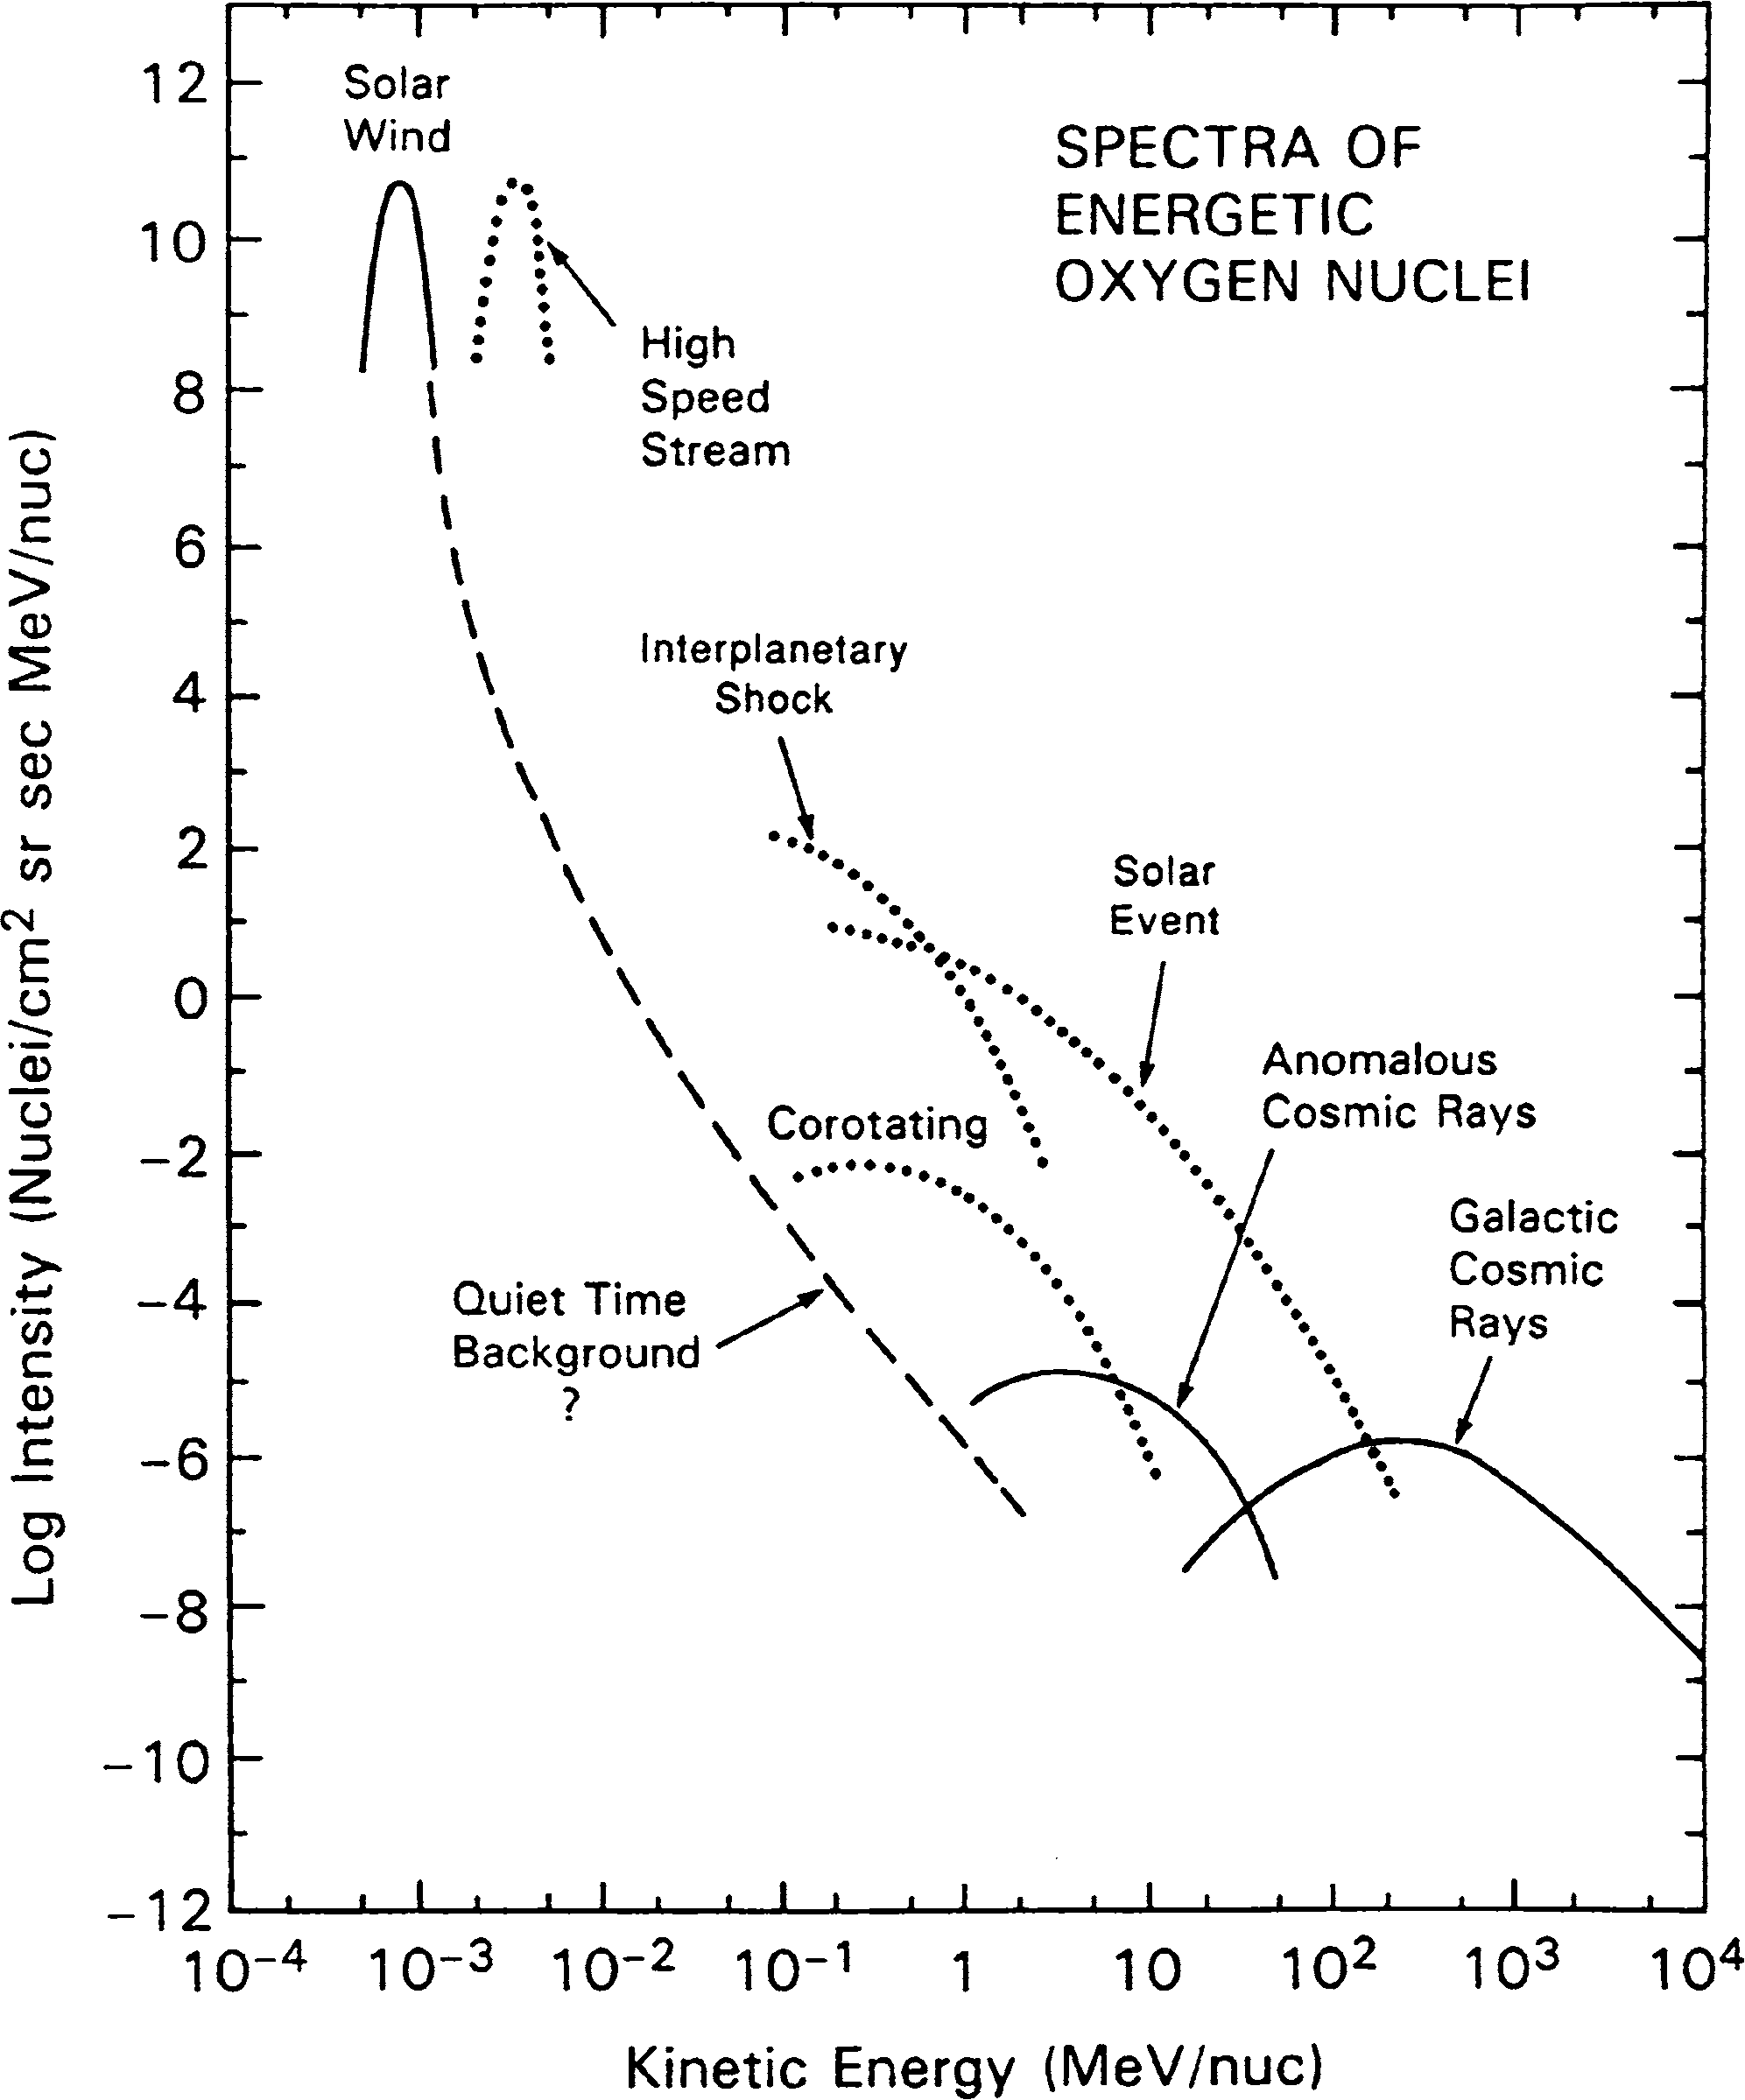
\includegraphics[width=0.6\linewidth]{images/heliospheric_energy_spectrum}
    \caption[Spectra of oxygen ions in the near-Earth interplanetary space]{Typical spectra of oxygen ions in the near-Earth interplanetary space, showing the contributions from different populations. Other particle species show similarly shaped spectra when plotted as a function of energy/nucleon (adapted from \url{http://helios.gsfc.nasa.gov/ace/gallery.html}, based on \cite{Mewaldt-2001}).}
    \label{fig:heliospheric_energy_spectrum}
\end{figure}
The by far most abundant population is the solar wind, a steady flow of plasma that is emitted from the Sun radially and fills the heliosphere. 
In the near-Earth space at one astronomical unit (\si{\AU}), the slow solar wind reaches typical speeds between \SIrange[range-phrase={\,and\,}]{300}{500}{\kilo\meter\per\second}.
Due to its low pressure, and therefore high plasma $\beta$, it carries the solar magnetic field with it and creates the \ac{IMF}.
As the Sun rotates, the \ac{IMF} forms an Archimedian spiral, which is named Parker spiral after Eugene N. \citet{Parker-1958}, who first developed this model of the solar wind.

However, our Sun is an active star, and thus the flow of particles is not simply constant. The variability is driven by the 11-year solar cycle, a recurring reversal of the solar magnetic field that is associated with enhancements in solar activity (solar maxmimum) due to the increased amount of magnetic stress and reconnection processes, and low-activity periods (solar minimum) inbetween.
Coronal holes, which are colder and therefore darker regions forming on the Sun, emit faster solar wind streams with speeds $\gtrsim \SI{600}{\kilo\meter\per\second}$. These \acp{HSS}, which are located right next to the (slow) solar wind in \autoref{fig:heliospheric_energy_spectrum}, then interact with the neighboring streams of slower wind due to their different Parker spiral curvature and form a \acl{SIR}\acused{SIR} \citep[\acs{SIR}, e.g.][]{Richardson-2018}. \acp{SIR} are flanked by interplanetary shocks on each side, the so-called forward and reverse shocks. If a coronal hole stays stable for a longer time, these interaction regions can be observed recurrently in each solar rotation (i.e., every $\sim$27 days when observed from Earth), in which case they are called \acp{CIR}.
Furthermore, active regions on the Sun can occasionally produce solar flares, sudden and intense emissions of light often associated with the release of high-energy ($\sim \si{\mega\electronvolt}$) \aclp{SEP}\acused{SEP} \citep[\acsp{SEP}, e.g.][]{Reames-1990}, as shown in the central area of \autoref{fig:heliospheric_energy_spectrum}.
Solar flares are believed to be powered by reconnection of magnetic field lines at the Sun, which leads to the release of energy and acceleration of particles.
These events often also coincide with the eruption of plasma from the solar corona in the form of a \ac{CME} at speeds up to a few thousands of \si{\kilo\meter\per\second}.
Just like the solar wind, \acp{CME} carry a magnetic field with them when they propagate away from the Sun. Due to their high speed, an interplanetary shock can form in front of the \ac{CME}, followed by a turbulent sheath region.
This shock can also be efficient at accelerating additional particles to higher energies, similar to \acp{SEP} accelerated directly at the Sun.

At the high end of the energy spectrum (\autoref{fig:heliospheric_energy_spectrum}), at \si{\mega\electronvolt} to  \si{\giga\electronvolt} energies, we find \acp{GCR}, charged particles originating from outside the heliosphere produced e.g. in stellar supernovae and entering it with a relatively constant and isotropic flux. 
Within the heliosphere, the flux of these high-energy particles is modulated by various effects: In the long term, the variation of the \ac{IMF} intensity during the 11-year solar cycle modulates the \ac{GCR} intensity observed in the inner solar system, so that the average \ac{GCR} flux is higher during solar minimum than at solar maximum \citep{Fisk-1980}. In addition, there are short-term modulations of \ac{GCR} due to magnetic structures in the solar wind, such as \acp{CME} and \acp{SIR}/\acp{CIR}. These are the so-called Forbush decreases, which will be the main focus of this thesis.

\section{Space Weather events and their detection}
\label{sec:spaceweather}

As defined by the U.S. National Space Weather Program, the term \textit{space weather} refers to ``conditions on the Sun and in the solar wind, magnetosphere, ionosphere and thermosphere that can influence the performance and reliability of space-borne and ground-based technological systems and endanger human life or health'' \parencite{OFCM-1995}.
The aforementioned large-scale heliospheric events, such as \acp{SEP}, \acp{CME} and \acp{CIR} are all relevant to space weather. For example, the increased radiation exposure due to accelerated energetic particles can be dangerous for astronauts. Additionally, the enhanced and turbulent magnetic fields impacting spacecraft or disturbing the Earth's magnetosphere in a so-called geomagnetic storm can cause disruptions of spacecraft electronics or of electricity grids on the ground.

Thus, the focus in space weather research is to enhance the understanding of these events in order to be able to more accurately predict their occurrence and propagation, including the onset time at Earth (or other locations in the solar system) and their intensity.
In the past, the investigation of heliospheric events has been mostly based on two kinds of measurements: First, remote sensing observations of the Sun and its vicinity, such as \ac{EUV} images, magnetograms and white-light coronagraph images, are available from spacecraft near Earth such as the \ac{SOHO} and the \ac{SDO}. Second, in situ observations, such as solar wind plasma measurements and magnetometers, can also be obtained from spacecraft located at the $L_1$ Lagrange point, including \ac{SOHO}, the \ac{ACE}, Wind, and the \ac{DSCOVR}.
In the last two decades, these observations have been complemented by in situ measurements from deep space heliophysics missions, such as from the two \ac{STEREO} spacecraft orbiting the Sun near \SI{1}{\AU} as well as the recent \ac{PSP} and \ac{SolO} missions, which are starting to provide valuable data from extremely close to the Sun with a larger variety of instruments and higher resolution than the Helios mission in the 1970s. In addition to observing the Sun and its corona, these missions also facilitate imaging observations of the interplanetary space using the wide field of view of their \acp{HI}. These can be used to directly track \acp{CME} all the way out to Earth (see \autoref{sec:stereohi}).

\section{Coronal mass ejections}
\label{sec:cmes}

As mentioned in Section \ref{sec:particles_heliosphere}, \acp{CME} are large-scale eruptions of plasma from the Sun that propagate outward into the heliosphere. They are often associated with flares and believed to be driven by reconnection of the coronal magnetic field \citep[see e.g.][for discussions on the triggering mechanism]{Forbes-2000,Kusano-2012}. \acp{CME} occur relatively frequently, on average every 4 days at solar minimum and 2.5 to 3 times per day at solar maximum \citep{Webb-1994}. The properties of \acp{CME} have a large variability: For example, their speeds can range between \SIrange[range-phrase={\,and\,}]{20}{2000}{\kilo\meter\per\second}, where the average is at about \SI{400}{\kilo\meter\per\second} and faster \acp{CME} are more likely to occur near solar maximum. Also, their longitudinal extent can differ: Very narrow (\SI{5}{\degree}) and very wide (\SI{120}{\degree}) cases have been observed, with the average being around \SI{50}{\degree} \citep{Cane-2000}. A classic example of a \ac{CME} observed by the \ac{SOHO} \ac{LASCO} C3 coronagraph is shown in \autoref{subfig:cme_remotesensing}. The black circle in the center of the coronagraph image is the occulter that covers the solar disk, and the \ac{CME} appears over the solar north pole as the source region is located north of the solar equator in this case (at $\sim\SI{30}{\degree}$ latitude).

\begin{figure}
    \centering
    \subfloat[\ac{CME} observed by the \ac{SOHO}/\ac{LASCO} C3 coronagraph on February 27, 2000.]{
    	\vspace{2mm}
	    %% Creator: Matplotlib, PGF backend
%%
%% To include the figure in your LaTeX document, write
%%   \input{<filename>.pgf}
%%
%% Make sure the required packages are loaded in your preamble
%%   \usepackage{pgf}
%%
%% and, on pdftex
%%   \usepackage[utf8]{inputenc}\DeclareUnicodeCharacter{2212}{-}
%%
%% or, on luatex and xetex
%%   \usepackage{unicode-math}
%%
%% Figures using additional raster images can only be included by \input if
%% they are in the same directory as the main LaTeX file. For loading figures
%% from other directories you can use the `import` package
%%   \usepackage{import}
%%
%% and then include the figures with
%%   \import{<path to file>}{<filename>.pgf}
%%
%% Matplotlib used the following preamble
%%   \usepackage{fontspec}
%%
\begingroup%
\makeatletter%
\begin{pgfpicture}%
\pgfpathrectangle{\pgfpointorigin}{\pgfqpoint{2.500000in}{2.500000in}}%
\pgfusepath{use as bounding box}%
\begin{pgfscope}%
\pgfsetbuttcap%
\pgfsetmiterjoin%
\definecolor{currentfill}{rgb}{1.000000,1.000000,1.000000}%
\pgfsetfillcolor{currentfill}%
\pgfsetlinewidth{0.000000pt}%
\definecolor{currentstroke}{rgb}{1.000000,1.000000,1.000000}%
\pgfsetstrokecolor{currentstroke}%
\pgfsetdash{}{0pt}%
\pgfpathmoveto{\pgfqpoint{0.000000in}{0.000000in}}%
\pgfpathlineto{\pgfqpoint{2.500000in}{0.000000in}}%
\pgfpathlineto{\pgfqpoint{2.500000in}{2.500000in}}%
\pgfpathlineto{\pgfqpoint{0.000000in}{2.500000in}}%
\pgfpathclose%
\pgfusepath{fill}%
\end{pgfscope}%
\begin{pgfscope}%
\pgfsetbuttcap%
\pgfsetmiterjoin%
\definecolor{currentfill}{rgb}{1.000000,1.000000,1.000000}%
\pgfsetfillcolor{currentfill}%
\pgfsetlinewidth{1.003750pt}%
\definecolor{currentstroke}{rgb}{1.000000,1.000000,1.000000}%
\pgfsetstrokecolor{currentstroke}%
\pgfsetdash{}{0pt}%
\pgfpathmoveto{\pgfqpoint{0.682546in}{0.638366in}}%
\pgfpathlineto{\pgfqpoint{2.350000in}{0.638366in}}%
\pgfpathlineto{\pgfqpoint{2.350000in}{0.638366in}}%
\pgfpathlineto{\pgfqpoint{2.350000in}{2.305819in}}%
\pgfpathlineto{\pgfqpoint{2.350000in}{2.305819in}}%
\pgfpathlineto{\pgfqpoint{0.682546in}{2.305819in}}%
\pgfpathlineto{\pgfqpoint{0.682546in}{2.305819in}}%
\pgfpathlineto{\pgfqpoint{0.682546in}{0.638366in}}%
\pgfusepath{stroke,fill}%
\end{pgfscope}%
\begin{pgfscope}%
\pgfpathmoveto{\pgfqpoint{0.682546in}{0.638366in}}%
\pgfpathlineto{\pgfqpoint{2.350000in}{0.638366in}}%
\pgfpathlineto{\pgfqpoint{2.350000in}{0.638366in}}%
\pgfpathlineto{\pgfqpoint{2.350000in}{2.305819in}}%
\pgfpathlineto{\pgfqpoint{2.350000in}{2.305819in}}%
\pgfpathlineto{\pgfqpoint{0.682546in}{2.305819in}}%
\pgfpathlineto{\pgfqpoint{0.682546in}{2.305819in}}%
\pgfpathlineto{\pgfqpoint{0.682546in}{0.638366in}}%
\pgfusepath{clip}%
\pgfsys@transformshift{0.682546in}{0.638366in}%
\pgftext[left,bottom]{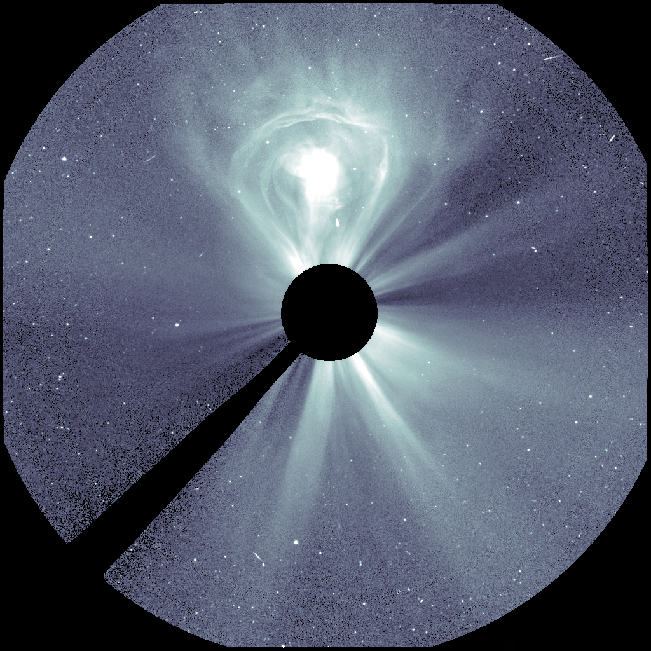
\includegraphics[interpolate=true,width=1.670000in,height=1.670000in]{plots/lightbulb_cme-img0.png}}%
\end{pgfscope}%
\begin{pgfscope}%
\pgfpathmoveto{\pgfqpoint{0.682546in}{0.638366in}}%
\pgfpathlineto{\pgfqpoint{2.350000in}{0.638366in}}%
\pgfpathlineto{\pgfqpoint{2.350000in}{0.638366in}}%
\pgfpathlineto{\pgfqpoint{2.350000in}{2.305819in}}%
\pgfpathlineto{\pgfqpoint{2.350000in}{2.305819in}}%
\pgfpathlineto{\pgfqpoint{0.682546in}{2.305819in}}%
\pgfpathlineto{\pgfqpoint{0.682546in}{2.305819in}}%
\pgfpathlineto{\pgfqpoint{0.682546in}{0.638366in}}%
\pgfusepath{clip}%
\pgfsetbuttcap%
\pgfsetmiterjoin%
\pgfsetlinewidth{0.501875pt}%
\definecolor{currentstroke}{rgb}{1.000000,1.000000,1.000000}%
\pgfsetstrokecolor{currentstroke}%
\pgfsetstrokeopacity{0.600000}%
\pgfsetdash{{0.500000pt}{0.825000pt}}{0.000000pt}%
\pgfpathmoveto{\pgfqpoint{1.000139in}{0.464583in}}%
\pgfpathlineto{\pgfqpoint{1.000139in}{2.478859in}}%
\pgfpathlineto{\pgfqpoint{1.000139in}{2.478859in}}%
\pgfusepath{stroke}%
\end{pgfscope}%
\begin{pgfscope}%
\pgfpathmoveto{\pgfqpoint{0.682546in}{0.638366in}}%
\pgfpathlineto{\pgfqpoint{2.350000in}{0.638366in}}%
\pgfpathlineto{\pgfqpoint{2.350000in}{0.638366in}}%
\pgfpathlineto{\pgfqpoint{2.350000in}{2.305819in}}%
\pgfpathlineto{\pgfqpoint{2.350000in}{2.305819in}}%
\pgfpathlineto{\pgfqpoint{0.682546in}{2.305819in}}%
\pgfpathlineto{\pgfqpoint{0.682546in}{2.305819in}}%
\pgfpathlineto{\pgfqpoint{0.682546in}{0.638366in}}%
\pgfusepath{clip}%
\pgfsetbuttcap%
\pgfsetmiterjoin%
\pgfsetlinewidth{0.501875pt}%
\definecolor{currentstroke}{rgb}{1.000000,1.000000,1.000000}%
\pgfsetstrokecolor{currentstroke}%
\pgfsetstrokeopacity{0.600000}%
\pgfsetdash{{0.500000pt}{0.825000pt}}{0.000000pt}%
\pgfpathmoveto{\pgfqpoint{1.524877in}{0.468531in}}%
\pgfpathlineto{\pgfqpoint{1.524877in}{2.475142in}}%
\pgfpathlineto{\pgfqpoint{1.524877in}{2.475142in}}%
\pgfusepath{stroke}%
\end{pgfscope}%
\begin{pgfscope}%
\pgfpathmoveto{\pgfqpoint{0.682546in}{0.638366in}}%
\pgfpathlineto{\pgfqpoint{2.350000in}{0.638366in}}%
\pgfpathlineto{\pgfqpoint{2.350000in}{0.638366in}}%
\pgfpathlineto{\pgfqpoint{2.350000in}{2.305819in}}%
\pgfpathlineto{\pgfqpoint{2.350000in}{2.305819in}}%
\pgfpathlineto{\pgfqpoint{0.682546in}{2.305819in}}%
\pgfpathlineto{\pgfqpoint{0.682546in}{2.305819in}}%
\pgfpathlineto{\pgfqpoint{0.682546in}{0.638366in}}%
\pgfusepath{clip}%
\pgfsetbuttcap%
\pgfsetmiterjoin%
\pgfsetlinewidth{0.501875pt}%
\definecolor{currentstroke}{rgb}{1.000000,1.000000,1.000000}%
\pgfsetstrokecolor{currentstroke}%
\pgfsetstrokeopacity{0.600000}%
\pgfsetdash{{0.500000pt}{0.825000pt}}{0.000000pt}%
\pgfpathmoveto{\pgfqpoint{2.049616in}{0.464583in}}%
\pgfpathlineto{\pgfqpoint{2.049616in}{2.478859in}}%
\pgfpathlineto{\pgfqpoint{2.049616in}{2.478859in}}%
\pgfusepath{stroke}%
\end{pgfscope}%
\begin{pgfscope}%
\pgfpathmoveto{\pgfqpoint{0.682546in}{0.638366in}}%
\pgfpathlineto{\pgfqpoint{2.350000in}{0.638366in}}%
\pgfpathlineto{\pgfqpoint{2.350000in}{0.638366in}}%
\pgfpathlineto{\pgfqpoint{2.350000in}{2.305819in}}%
\pgfpathlineto{\pgfqpoint{2.350000in}{2.305819in}}%
\pgfpathlineto{\pgfqpoint{0.682546in}{2.305819in}}%
\pgfpathlineto{\pgfqpoint{0.682546in}{2.305819in}}%
\pgfpathlineto{\pgfqpoint{0.682546in}{0.638366in}}%
\pgfusepath{clip}%
\pgfsetbuttcap%
\pgfsetmiterjoin%
\pgfsetlinewidth{0.501875pt}%
\definecolor{currentstroke}{rgb}{1.000000,1.000000,1.000000}%
\pgfsetstrokecolor{currentstroke}%
\pgfsetstrokeopacity{0.600000}%
\pgfsetdash{{0.500000pt}{0.825000pt}}{0.000000pt}%
\pgfpathmoveto{\pgfqpoint{0.512894in}{0.970044in}}%
\pgfpathlineto{\pgfqpoint{0.742840in}{0.973019in}}%
\pgfpathlineto{\pgfqpoint{0.970549in}{0.975225in}}%
\pgfpathlineto{\pgfqpoint{1.196684in}{0.976676in}}%
\pgfpathlineto{\pgfqpoint{1.421892in}{0.977384in}}%
\pgfpathlineto{\pgfqpoint{1.646810in}{0.977353in}}%
\pgfpathlineto{\pgfqpoint{1.872072in}{0.976583in}}%
\pgfpathlineto{\pgfqpoint{2.098314in}{0.975068in}}%
\pgfpathlineto{\pgfqpoint{2.326185in}{0.972799in}}%
\pgfpathlineto{\pgfqpoint{2.519506in}{0.970295in}}%
\pgfpathlineto{\pgfqpoint{2.519506in}{0.970295in}}%
\pgfusepath{stroke}%
\end{pgfscope}%
\begin{pgfscope}%
\pgfpathmoveto{\pgfqpoint{0.682546in}{0.638366in}}%
\pgfpathlineto{\pgfqpoint{2.350000in}{0.638366in}}%
\pgfpathlineto{\pgfqpoint{2.350000in}{0.638366in}}%
\pgfpathlineto{\pgfqpoint{2.350000in}{2.305819in}}%
\pgfpathlineto{\pgfqpoint{2.350000in}{2.305819in}}%
\pgfpathlineto{\pgfqpoint{0.682546in}{2.305819in}}%
\pgfpathlineto{\pgfqpoint{0.682546in}{2.305819in}}%
\pgfpathlineto{\pgfqpoint{0.682546in}{0.638366in}}%
\pgfusepath{clip}%
\pgfsetbuttcap%
\pgfsetmiterjoin%
\pgfsetlinewidth{0.501875pt}%
\definecolor{currentstroke}{rgb}{1.000000,1.000000,1.000000}%
\pgfsetstrokecolor{currentstroke}%
\pgfsetstrokeopacity{0.600000}%
\pgfsetdash{{0.500000pt}{0.825000pt}}{0.000000pt}%
\pgfpathmoveto{\pgfqpoint{0.512894in}{1.502199in}}%
\pgfpathlineto{\pgfqpoint{2.519506in}{1.502199in}}%
\pgfpathlineto{\pgfqpoint{2.519506in}{1.502199in}}%
\pgfusepath{stroke}%
\end{pgfscope}%
\begin{pgfscope}%
\pgfpathmoveto{\pgfqpoint{0.682546in}{0.638366in}}%
\pgfpathlineto{\pgfqpoint{2.350000in}{0.638366in}}%
\pgfpathlineto{\pgfqpoint{2.350000in}{0.638366in}}%
\pgfpathlineto{\pgfqpoint{2.350000in}{2.305819in}}%
\pgfpathlineto{\pgfqpoint{2.350000in}{2.305819in}}%
\pgfpathlineto{\pgfqpoint{0.682546in}{2.305819in}}%
\pgfpathlineto{\pgfqpoint{0.682546in}{2.305819in}}%
\pgfpathlineto{\pgfqpoint{0.682546in}{0.638366in}}%
\pgfusepath{clip}%
\pgfsetbuttcap%
\pgfsetmiterjoin%
\pgfsetlinewidth{0.501875pt}%
\definecolor{currentstroke}{rgb}{1.000000,1.000000,1.000000}%
\pgfsetstrokecolor{currentstroke}%
\pgfsetstrokeopacity{0.600000}%
\pgfsetdash{{0.500000pt}{0.825000pt}}{0.000000pt}%
\pgfpathmoveto{\pgfqpoint{0.512894in}{2.034355in}}%
\pgfpathlineto{\pgfqpoint{0.742840in}{2.031380in}}%
\pgfpathlineto{\pgfqpoint{0.970549in}{2.029174in}}%
\pgfpathlineto{\pgfqpoint{1.196684in}{2.027723in}}%
\pgfpathlineto{\pgfqpoint{1.421892in}{2.027015in}}%
\pgfpathlineto{\pgfqpoint{1.646810in}{2.027046in}}%
\pgfpathlineto{\pgfqpoint{1.872072in}{2.027816in}}%
\pgfpathlineto{\pgfqpoint{2.098314in}{2.029331in}}%
\pgfpathlineto{\pgfqpoint{2.326185in}{2.031600in}}%
\pgfpathlineto{\pgfqpoint{2.519506in}{2.034104in}}%
\pgfpathlineto{\pgfqpoint{2.519506in}{2.034104in}}%
\pgfusepath{stroke}%
\end{pgfscope}%
\begin{pgfscope}%
\pgfsetbuttcap%
\pgfsetroundjoin%
\pgfsetlinewidth{0.803000pt}%
\definecolor{currentstroke}{rgb}{0.000000,0.000000,0.000000}%
\pgfsetstrokecolor{currentstroke}%
\pgfsetdash{}{0pt}%
\pgfsys@defobject{currentmarker}{\pgfqpoint{-0.000000in}{-0.048611in}}{\pgfqpoint{0.000000in}{0.000000in}}{%
\pgfpathmoveto{\pgfqpoint{0.000000in}{0.000000in}}%
\pgfpathlineto{\pgfqpoint{-0.000000in}{-0.048611in}}%
\pgfusepath{stroke}%
}%
\begin{pgfscope}%
\pgfsys@transformshift{1.000139in}{0.638366in}%
\pgfsys@useobject{currentmarker}{}%
\end{pgfscope}%
\begin{pgfscope}%
\pgfsys@transformshift{1.000139in}{0.638366in}%
\pgfsys@useobject{currentmarker}{}%
\end{pgfscope}%
\end{pgfscope}%
\begin{pgfscope}%
\pgfsetbuttcap%
\pgfsetroundjoin%
\pgfsetlinewidth{0.803000pt}%
\definecolor{currentstroke}{rgb}{0.000000,0.000000,0.000000}%
\pgfsetstrokecolor{currentstroke}%
\pgfsetdash{}{0pt}%
\pgfsys@defobject{currentmarker}{\pgfqpoint{-0.000000in}{-0.048611in}}{\pgfqpoint{0.000000in}{0.000000in}}{%
\pgfpathmoveto{\pgfqpoint{0.000000in}{0.000000in}}%
\pgfpathlineto{\pgfqpoint{-0.000000in}{-0.048611in}}%
\pgfusepath{stroke}%
}%
\begin{pgfscope}%
\pgfsys@transformshift{1.524877in}{0.638366in}%
\pgfsys@useobject{currentmarker}{}%
\end{pgfscope}%
\begin{pgfscope}%
\pgfsys@transformshift{1.524877in}{0.638366in}%
\pgfsys@useobject{currentmarker}{}%
\end{pgfscope}%
\end{pgfscope}%
\begin{pgfscope}%
\pgfsetbuttcap%
\pgfsetroundjoin%
\pgfsetlinewidth{0.803000pt}%
\definecolor{currentstroke}{rgb}{0.000000,0.000000,0.000000}%
\pgfsetstrokecolor{currentstroke}%
\pgfsetdash{}{0pt}%
\pgfsys@defobject{currentmarker}{\pgfqpoint{-0.000000in}{-0.048611in}}{\pgfqpoint{0.000000in}{0.000000in}}{%
\pgfpathmoveto{\pgfqpoint{0.000000in}{0.000000in}}%
\pgfpathlineto{\pgfqpoint{-0.000000in}{-0.048611in}}%
\pgfusepath{stroke}%
}%
\begin{pgfscope}%
\pgfsys@transformshift{2.049616in}{0.638366in}%
\pgfsys@useobject{currentmarker}{}%
\end{pgfscope}%
\begin{pgfscope}%
\pgfsys@transformshift{2.049616in}{0.638366in}%
\pgfsys@useobject{currentmarker}{}%
\end{pgfscope}%
\end{pgfscope}%
\begin{pgfscope}%
\pgfsetbuttcap%
\pgfsetroundjoin%
\pgfsetlinewidth{0.803000pt}%
\definecolor{currentstroke}{rgb}{0.000000,0.000000,0.000000}%
\pgfsetstrokecolor{currentstroke}%
\pgfsetdash{}{0pt}%
\pgfsys@defobject{currentmarker}{\pgfqpoint{0.000000in}{0.000000in}}{\pgfqpoint{0.000000in}{0.048611in}}{%
\pgfpathmoveto{\pgfqpoint{0.000000in}{0.000000in}}%
\pgfpathlineto{\pgfqpoint{0.000000in}{0.048611in}}%
\pgfusepath{stroke}%
}%
\begin{pgfscope}%
\pgfsys@transformshift{1.000139in}{2.305819in}%
\pgfsys@useobject{currentmarker}{}%
\end{pgfscope}%
\begin{pgfscope}%
\pgfsys@transformshift{1.000139in}{2.305819in}%
\pgfsys@useobject{currentmarker}{}%
\end{pgfscope}%
\end{pgfscope}%
\begin{pgfscope}%
\pgfsetbuttcap%
\pgfsetroundjoin%
\pgfsetlinewidth{0.803000pt}%
\definecolor{currentstroke}{rgb}{0.000000,0.000000,0.000000}%
\pgfsetstrokecolor{currentstroke}%
\pgfsetdash{}{0pt}%
\pgfsys@defobject{currentmarker}{\pgfqpoint{0.000000in}{0.000000in}}{\pgfqpoint{0.000000in}{0.048611in}}{%
\pgfpathmoveto{\pgfqpoint{0.000000in}{0.000000in}}%
\pgfpathlineto{\pgfqpoint{0.000000in}{0.048611in}}%
\pgfusepath{stroke}%
}%
\begin{pgfscope}%
\pgfsys@transformshift{1.524877in}{2.305819in}%
\pgfsys@useobject{currentmarker}{}%
\end{pgfscope}%
\begin{pgfscope}%
\pgfsys@transformshift{1.524877in}{2.305819in}%
\pgfsys@useobject{currentmarker}{}%
\end{pgfscope}%
\end{pgfscope}%
\begin{pgfscope}%
\pgfsetbuttcap%
\pgfsetroundjoin%
\pgfsetlinewidth{0.803000pt}%
\definecolor{currentstroke}{rgb}{0.000000,0.000000,0.000000}%
\pgfsetstrokecolor{currentstroke}%
\pgfsetdash{}{0pt}%
\pgfsys@defobject{currentmarker}{\pgfqpoint{0.000000in}{0.000000in}}{\pgfqpoint{0.000000in}{0.048611in}}{%
\pgfpathmoveto{\pgfqpoint{0.000000in}{0.000000in}}%
\pgfpathlineto{\pgfqpoint{0.000000in}{0.048611in}}%
\pgfusepath{stroke}%
}%
\begin{pgfscope}%
\pgfsys@transformshift{2.049616in}{2.305819in}%
\pgfsys@useobject{currentmarker}{}%
\end{pgfscope}%
\begin{pgfscope}%
\pgfsys@transformshift{2.049616in}{2.305819in}%
\pgfsys@useobject{currentmarker}{}%
\end{pgfscope}%
\end{pgfscope}%
\begin{pgfscope}%
\definecolor{textcolor}{rgb}{0.000000,0.000000,0.000000}%
\pgfsetstrokecolor{textcolor}%
\pgfsetfillcolor{textcolor}%
\pgftext[x=1.000139in,y=0.402254in,,bottom]{\color{textcolor}\rmfamily\fontsize{10.000000}{12.000000}\selectfont \(\displaystyle -5^\circ\)}%
\end{pgfscope}%
\begin{pgfscope}%
\definecolor{textcolor}{rgb}{0.000000,0.000000,0.000000}%
\pgfsetstrokecolor{textcolor}%
\pgfsetfillcolor{textcolor}%
\pgftext[x=1.524877in,y=0.402254in,,bottom]{\color{textcolor}\rmfamily\fontsize{10.000000}{12.000000}\selectfont \(\displaystyle 0^\circ\)}%
\end{pgfscope}%
\begin{pgfscope}%
\definecolor{textcolor}{rgb}{0.000000,0.000000,0.000000}%
\pgfsetstrokecolor{textcolor}%
\pgfsetfillcolor{textcolor}%
\pgftext[x=2.049616in,y=0.402254in,,bottom]{\color{textcolor}\rmfamily\fontsize{10.000000}{12.000000}\selectfont \(\displaystyle 5^\circ\)}%
\end{pgfscope}%
\begin{pgfscope}%
\pgfsetbuttcap%
\pgfsetroundjoin%
\pgfsetlinewidth{0.803000pt}%
\definecolor{currentstroke}{rgb}{0.000000,0.000000,0.000000}%
\pgfsetstrokecolor{currentstroke}%
\pgfsetdash{}{0pt}%
\pgfsys@defobject{currentmarker}{\pgfqpoint{-0.048608in}{-0.000589in}}{\pgfqpoint{0.000000in}{0.000000in}}{%
\pgfpathmoveto{\pgfqpoint{0.000000in}{0.000000in}}%
\pgfpathlineto{\pgfqpoint{-0.048608in}{-0.000589in}}%
\pgfusepath{stroke}%
}%
\begin{pgfscope}%
\pgfsys@transformshift{0.682546in}{0.972312in}%
\pgfsys@useobject{currentmarker}{}%
\end{pgfscope}%
\begin{pgfscope}%
\pgfsys@transformshift{0.682546in}{0.972312in}%
\pgfsys@useobject{currentmarker}{}%
\end{pgfscope}%
\end{pgfscope}%
\begin{pgfscope}%
\pgfsetbuttcap%
\pgfsetroundjoin%
\pgfsetlinewidth{0.803000pt}%
\definecolor{currentstroke}{rgb}{0.000000,0.000000,0.000000}%
\pgfsetstrokecolor{currentstroke}%
\pgfsetdash{}{0pt}%
\pgfsys@defobject{currentmarker}{\pgfqpoint{-0.048611in}{0.000000in}}{\pgfqpoint{0.000000in}{0.000000in}}{%
\pgfpathmoveto{\pgfqpoint{0.000000in}{0.000000in}}%
\pgfpathlineto{\pgfqpoint{-0.048611in}{0.000000in}}%
\pgfusepath{stroke}%
}%
\begin{pgfscope}%
\pgfsys@transformshift{0.682546in}{1.502199in}%
\pgfsys@useobject{currentmarker}{}%
\end{pgfscope}%
\begin{pgfscope}%
\pgfsys@transformshift{0.682546in}{1.502199in}%
\pgfsys@useobject{currentmarker}{}%
\end{pgfscope}%
\end{pgfscope}%
\begin{pgfscope}%
\pgfsetbuttcap%
\pgfsetroundjoin%
\pgfsetlinewidth{0.803000pt}%
\definecolor{currentstroke}{rgb}{0.000000,0.000000,0.000000}%
\pgfsetstrokecolor{currentstroke}%
\pgfsetdash{}{0pt}%
\pgfsys@defobject{currentmarker}{\pgfqpoint{-0.048608in}{0.000000in}}{\pgfqpoint{0.000000in}{0.000589in}}{%
\pgfpathmoveto{\pgfqpoint{0.000000in}{0.000000in}}%
\pgfpathlineto{\pgfqpoint{-0.048608in}{0.000589in}}%
\pgfusepath{stroke}%
}%
\begin{pgfscope}%
\pgfsys@transformshift{0.682546in}{2.032087in}%
\pgfsys@useobject{currentmarker}{}%
\end{pgfscope}%
\begin{pgfscope}%
\pgfsys@transformshift{0.682546in}{2.032087in}%
\pgfsys@useobject{currentmarker}{}%
\end{pgfscope}%
\end{pgfscope}%
\begin{pgfscope}%
\pgfsetbuttcap%
\pgfsetroundjoin%
\pgfsetlinewidth{0.803000pt}%
\definecolor{currentstroke}{rgb}{0.000000,0.000000,0.000000}%
\pgfsetstrokecolor{currentstroke}%
\pgfsetdash{}{0pt}%
\pgfsys@defobject{currentmarker}{\pgfqpoint{0.000000in}{-0.000582in}}{\pgfqpoint{0.048608in}{0.000000in}}{%
\pgfpathmoveto{\pgfqpoint{0.000000in}{0.000000in}}%
\pgfpathlineto{\pgfqpoint{0.048608in}{-0.000582in}}%
\pgfusepath{stroke}%
}%
\begin{pgfscope}%
\pgfsys@transformshift{2.350000in}{0.972519in}%
\pgfsys@useobject{currentmarker}{}%
\end{pgfscope}%
\begin{pgfscope}%
\pgfsys@transformshift{2.350000in}{0.972519in}%
\pgfsys@useobject{currentmarker}{}%
\end{pgfscope}%
\end{pgfscope}%
\begin{pgfscope}%
\pgfsetbuttcap%
\pgfsetroundjoin%
\pgfsetlinewidth{0.803000pt}%
\definecolor{currentstroke}{rgb}{0.000000,0.000000,0.000000}%
\pgfsetstrokecolor{currentstroke}%
\pgfsetdash{}{0pt}%
\pgfsys@defobject{currentmarker}{\pgfqpoint{0.000000in}{0.000000in}}{\pgfqpoint{0.048611in}{0.000000in}}{%
\pgfpathmoveto{\pgfqpoint{0.000000in}{0.000000in}}%
\pgfpathlineto{\pgfqpoint{0.048611in}{0.000000in}}%
\pgfusepath{stroke}%
}%
\begin{pgfscope}%
\pgfsys@transformshift{2.350000in}{1.502199in}%
\pgfsys@useobject{currentmarker}{}%
\end{pgfscope}%
\begin{pgfscope}%
\pgfsys@transformshift{2.350000in}{1.502199in}%
\pgfsys@useobject{currentmarker}{}%
\end{pgfscope}%
\end{pgfscope}%
\begin{pgfscope}%
\pgfsetbuttcap%
\pgfsetroundjoin%
\pgfsetlinewidth{0.803000pt}%
\definecolor{currentstroke}{rgb}{0.000000,0.000000,0.000000}%
\pgfsetstrokecolor{currentstroke}%
\pgfsetdash{}{0pt}%
\pgfsys@defobject{currentmarker}{\pgfqpoint{0.000000in}{0.000000in}}{\pgfqpoint{0.048608in}{0.000582in}}{%
\pgfpathmoveto{\pgfqpoint{0.000000in}{0.000000in}}%
\pgfpathlineto{\pgfqpoint{0.048608in}{0.000582in}}%
\pgfusepath{stroke}%
}%
\begin{pgfscope}%
\pgfsys@transformshift{2.350000in}{2.031880in}%
\pgfsys@useobject{currentmarker}{}%
\end{pgfscope}%
\begin{pgfscope}%
\pgfsys@transformshift{2.350000in}{2.031880in}%
\pgfsys@useobject{currentmarker}{}%
\end{pgfscope}%
\end{pgfscope}%
\begin{pgfscope}%
\definecolor{textcolor}{rgb}{0.000000,0.000000,0.000000}%
\pgfsetstrokecolor{textcolor}%
\pgfsetfillcolor{textcolor}%
\pgftext[x=0.585324in,y=1.962643in,right,bottom]{\color{textcolor}\rmfamily\fontsize{10.000000}{12.000000}\selectfont \(\displaystyle 5^\circ\)}%
\end{pgfscope}%
\begin{pgfscope}%
\definecolor{textcolor}{rgb}{0.000000,0.000000,0.000000}%
\pgfsetstrokecolor{textcolor}%
\pgfsetfillcolor{textcolor}%
\pgftext[x=0.585324in,y=1.432755in,right,bottom]{\color{textcolor}\rmfamily\fontsize{10.000000}{12.000000}\selectfont \(\displaystyle 0^\circ\)}%
\end{pgfscope}%
\begin{pgfscope}%
\definecolor{textcolor}{rgb}{0.000000,0.000000,0.000000}%
\pgfsetstrokecolor{textcolor}%
\pgfsetfillcolor{textcolor}%
\pgftext[x=0.585324in,y=0.902867in,right,bottom]{\color{textcolor}\rmfamily\fontsize{10.000000}{12.000000}\selectfont \(\displaystyle -5^\circ\)}%
\end{pgfscope}%
\begin{pgfscope}%
\definecolor{textcolor}{rgb}{0.000000,0.000000,0.000000}%
\pgfsetstrokecolor{textcolor}%
\pgfsetfillcolor{textcolor}%
\pgftext[x=1.516273in,y=0.263366in,,]{\color{textcolor}\rmfamily\fontsize{10.000000}{12.000000}\selectfont Helioprojective Longitude [°]}%
\end{pgfscope}%
\begin{pgfscope}%
\definecolor{textcolor}{rgb}{0.000000,0.000000,0.000000}%
\pgfsetstrokecolor{textcolor}%
\pgfsetfillcolor{textcolor}%
\pgftext[x=0.239837in, y=0.648134in, left, base,rotate=90.000000]{\color{textcolor}\rmfamily\fontsize{10.000000}{12.000000}\selectfont Helioprojective Latitude [°]}%
\end{pgfscope}%
\begin{pgfscope}%
\pgfsetrectcap%
\pgfsetroundjoin%
\pgfsetlinewidth{0.803000pt}%
\definecolor{currentstroke}{rgb}{0.000000,0.000000,0.000000}%
\pgfsetstrokecolor{currentstroke}%
\pgfsetdash{}{0pt}%
\pgfpathmoveto{\pgfqpoint{0.682546in}{0.638366in}}%
\pgfpathlineto{\pgfqpoint{2.350000in}{0.638366in}}%
\pgfusepath{stroke}%
\end{pgfscope}%
\begin{pgfscope}%
\pgfsetrectcap%
\pgfsetroundjoin%
\pgfsetlinewidth{0.803000pt}%
\definecolor{currentstroke}{rgb}{0.000000,0.000000,0.000000}%
\pgfsetstrokecolor{currentstroke}%
\pgfsetdash{}{0pt}%
\pgfpathmoveto{\pgfqpoint{2.350000in}{0.638366in}}%
\pgfpathlineto{\pgfqpoint{2.350000in}{2.305819in}}%
\pgfusepath{stroke}%
\end{pgfscope}%
\begin{pgfscope}%
\pgfsetrectcap%
\pgfsetroundjoin%
\pgfsetlinewidth{0.803000pt}%
\definecolor{currentstroke}{rgb}{0.000000,0.000000,0.000000}%
\pgfsetstrokecolor{currentstroke}%
\pgfsetdash{}{0pt}%
\pgfpathmoveto{\pgfqpoint{2.350000in}{2.305819in}}%
\pgfpathlineto{\pgfqpoint{0.682546in}{2.305819in}}%
\pgfusepath{stroke}%
\end{pgfscope}%
\begin{pgfscope}%
\pgfsetrectcap%
\pgfsetroundjoin%
\pgfsetlinewidth{0.803000pt}%
\definecolor{currentstroke}{rgb}{0.000000,0.000000,0.000000}%
\pgfsetstrokecolor{currentstroke}%
\pgfsetdash{}{0pt}%
\pgfpathmoveto{\pgfqpoint{0.682546in}{2.305819in}}%
\pgfpathlineto{\pgfqpoint{0.682546in}{0.638366in}}%
\pgfusepath{stroke}%
\end{pgfscope}%
\begin{pgfscope}%
\definecolor{textcolor}{rgb}{0.000000,0.000000,0.000000}%
\pgfsetstrokecolor{textcolor}%
\pgfsetfillcolor{textcolor}%
\pgftext[x=0.835106in, y=2.569619in, left, base]{\color{textcolor}\rmfamily\fontsize{12.000000}{14.400000}\selectfont SOHO/LASCO-C3}%
\end{pgfscope}%
\begin{pgfscope}%
\definecolor{textcolor}{rgb}{0.000000,0.000000,0.000000}%
\pgfsetstrokecolor{textcolor}%
\pgfsetfillcolor{textcolor}%
\pgftext[x=0.817773in, y=2.389153in, left, base]{\color{textcolor}\rmfamily\fontsize{12.000000}{14.400000}\selectfont 2000-02-27 07:42:05}%
\end{pgfscope}%
\end{pgfpicture}%
\makeatother%
\endgroup%

	    \label{subfig:cme_remotesensing}
	}
	\hspace{5mm}
	\subfloat[\acs{ICME} signatures in \ac{ACE} magnetic field and plasma data on April 17, 1999.]{
		%% Creator: Matplotlib, PGF backend
%%
%% To include the figure in your LaTeX document, write
%%   \input{<filename>.pgf}
%%
%% Make sure the required packages are loaded in your preamble
%%   \usepackage{pgf}
%%
%% and, on pdftex
%%   \usepackage[utf8]{inputenc}\DeclareUnicodeCharacter{2212}{-}
%%
%% or, on luatex and xetex
%%   \usepackage{unicode-math}
%%
%% Figures using additional raster images can only be included by \input if
%% they are in the same directory as the main LaTeX file. For loading figures
%% from other directories you can use the `import` package
%%   \usepackage{import}
%%
%% and then include the figures with
%%   \import{<path to file>}{<filename>.pgf}
%%
%% Matplotlib used the following preamble
%%   \usepackage{fontspec}
%%
\begingroup%
\makeatletter%
\begin{pgfpicture}%
\pgfpathrectangle{\pgfpointorigin}{\pgfqpoint{2.500000in}{2.500000in}}%
\pgfusepath{use as bounding box, clip}%
\begin{pgfscope}%
\pgfsetbuttcap%
\pgfsetmiterjoin%
\definecolor{currentfill}{rgb}{1.000000,1.000000,1.000000}%
\pgfsetfillcolor{currentfill}%
\pgfsetlinewidth{0.000000pt}%
\definecolor{currentstroke}{rgb}{1.000000,1.000000,1.000000}%
\pgfsetstrokecolor{currentstroke}%
\pgfsetdash{}{0pt}%
\pgfpathmoveto{\pgfqpoint{0.000000in}{0.000000in}}%
\pgfpathlineto{\pgfqpoint{2.500000in}{0.000000in}}%
\pgfpathlineto{\pgfqpoint{2.500000in}{2.500000in}}%
\pgfpathlineto{\pgfqpoint{0.000000in}{2.500000in}}%
\pgfpathclose%
\pgfusepath{fill}%
\end{pgfscope}%
\begin{pgfscope}%
\pgfsetbuttcap%
\pgfsetmiterjoin%
\definecolor{currentfill}{rgb}{1.000000,1.000000,1.000000}%
\pgfsetfillcolor{currentfill}%
\pgfsetlinewidth{0.000000pt}%
\definecolor{currentstroke}{rgb}{0.000000,0.000000,0.000000}%
\pgfsetstrokecolor{currentstroke}%
\pgfsetstrokeopacity{0.000000}%
\pgfsetdash{}{0pt}%
\pgfpathmoveto{\pgfqpoint{0.588735in}{1.707388in}}%
\pgfpathlineto{\pgfqpoint{1.879401in}{1.707388in}}%
\pgfpathlineto{\pgfqpoint{1.879401in}{2.347404in}}%
\pgfpathlineto{\pgfqpoint{0.588735in}{2.347404in}}%
\pgfpathclose%
\pgfusepath{fill}%
\end{pgfscope}%
\begin{pgfscope}%
\pgfsetbuttcap%
\pgfsetroundjoin%
\definecolor{currentfill}{rgb}{0.000000,0.000000,0.000000}%
\pgfsetfillcolor{currentfill}%
\pgfsetlinewidth{0.803000pt}%
\definecolor{currentstroke}{rgb}{0.000000,0.000000,0.000000}%
\pgfsetstrokecolor{currentstroke}%
\pgfsetdash{}{0pt}%
\pgfsys@defobject{currentmarker}{\pgfqpoint{0.000000in}{-0.048611in}}{\pgfqpoint{0.000000in}{0.000000in}}{%
\pgfpathmoveto{\pgfqpoint{0.000000in}{0.000000in}}%
\pgfpathlineto{\pgfqpoint{0.000000in}{-0.048611in}}%
\pgfusepath{stroke,fill}%
}%
\begin{pgfscope}%
\pgfsys@transformshift{1.134103in}{1.707388in}%
\pgfsys@useobject{currentmarker}{}%
\end{pgfscope}%
\end{pgfscope}%
\begin{pgfscope}%
\pgfsetbuttcap%
\pgfsetroundjoin%
\definecolor{currentfill}{rgb}{0.000000,0.000000,0.000000}%
\pgfsetfillcolor{currentfill}%
\pgfsetlinewidth{0.803000pt}%
\definecolor{currentstroke}{rgb}{0.000000,0.000000,0.000000}%
\pgfsetstrokecolor{currentstroke}%
\pgfsetdash{}{0pt}%
\pgfsys@defobject{currentmarker}{\pgfqpoint{0.000000in}{-0.048611in}}{\pgfqpoint{0.000000in}{0.000000in}}{%
\pgfpathmoveto{\pgfqpoint{0.000000in}{0.000000in}}%
\pgfpathlineto{\pgfqpoint{0.000000in}{-0.048611in}}%
\pgfusepath{stroke,fill}%
}%
\begin{pgfscope}%
\pgfsys@transformshift{1.821211in}{1.707388in}%
\pgfsys@useobject{currentmarker}{}%
\end{pgfscope}%
\end{pgfscope}%
\begin{pgfscope}%
\pgfsetbuttcap%
\pgfsetroundjoin%
\definecolor{currentfill}{rgb}{0.000000,0.000000,0.000000}%
\pgfsetfillcolor{currentfill}%
\pgfsetlinewidth{0.602250pt}%
\definecolor{currentstroke}{rgb}{0.000000,0.000000,0.000000}%
\pgfsetstrokecolor{currentstroke}%
\pgfsetdash{}{0pt}%
\pgfsys@defobject{currentmarker}{\pgfqpoint{0.000000in}{-0.027778in}}{\pgfqpoint{0.000000in}{0.000000in}}{%
\pgfpathmoveto{\pgfqpoint{0.000000in}{0.000000in}}%
\pgfpathlineto{\pgfqpoint{0.000000in}{-0.027778in}}%
\pgfusepath{stroke,fill}%
}%
\begin{pgfscope}%
\pgfsys@transformshift{0.618772in}{1.707388in}%
\pgfsys@useobject{currentmarker}{}%
\end{pgfscope}%
\end{pgfscope}%
\begin{pgfscope}%
\pgfsetbuttcap%
\pgfsetroundjoin%
\definecolor{currentfill}{rgb}{0.000000,0.000000,0.000000}%
\pgfsetfillcolor{currentfill}%
\pgfsetlinewidth{0.602250pt}%
\definecolor{currentstroke}{rgb}{0.000000,0.000000,0.000000}%
\pgfsetstrokecolor{currentstroke}%
\pgfsetdash{}{0pt}%
\pgfsys@defobject{currentmarker}{\pgfqpoint{0.000000in}{-0.027778in}}{\pgfqpoint{0.000000in}{0.000000in}}{%
\pgfpathmoveto{\pgfqpoint{0.000000in}{0.000000in}}%
\pgfpathlineto{\pgfqpoint{0.000000in}{-0.027778in}}%
\pgfusepath{stroke,fill}%
}%
\begin{pgfscope}%
\pgfsys@transformshift{0.790549in}{1.707388in}%
\pgfsys@useobject{currentmarker}{}%
\end{pgfscope}%
\end{pgfscope}%
\begin{pgfscope}%
\pgfsetbuttcap%
\pgfsetroundjoin%
\definecolor{currentfill}{rgb}{0.000000,0.000000,0.000000}%
\pgfsetfillcolor{currentfill}%
\pgfsetlinewidth{0.602250pt}%
\definecolor{currentstroke}{rgb}{0.000000,0.000000,0.000000}%
\pgfsetstrokecolor{currentstroke}%
\pgfsetdash{}{0pt}%
\pgfsys@defobject{currentmarker}{\pgfqpoint{0.000000in}{-0.027778in}}{\pgfqpoint{0.000000in}{0.000000in}}{%
\pgfpathmoveto{\pgfqpoint{0.000000in}{0.000000in}}%
\pgfpathlineto{\pgfqpoint{0.000000in}{-0.027778in}}%
\pgfusepath{stroke,fill}%
}%
\begin{pgfscope}%
\pgfsys@transformshift{0.962326in}{1.707388in}%
\pgfsys@useobject{currentmarker}{}%
\end{pgfscope}%
\end{pgfscope}%
\begin{pgfscope}%
\pgfsetbuttcap%
\pgfsetroundjoin%
\definecolor{currentfill}{rgb}{0.000000,0.000000,0.000000}%
\pgfsetfillcolor{currentfill}%
\pgfsetlinewidth{0.602250pt}%
\definecolor{currentstroke}{rgb}{0.000000,0.000000,0.000000}%
\pgfsetstrokecolor{currentstroke}%
\pgfsetdash{}{0pt}%
\pgfsys@defobject{currentmarker}{\pgfqpoint{0.000000in}{-0.027778in}}{\pgfqpoint{0.000000in}{0.000000in}}{%
\pgfpathmoveto{\pgfqpoint{0.000000in}{0.000000in}}%
\pgfpathlineto{\pgfqpoint{0.000000in}{-0.027778in}}%
\pgfusepath{stroke,fill}%
}%
\begin{pgfscope}%
\pgfsys@transformshift{1.305880in}{1.707388in}%
\pgfsys@useobject{currentmarker}{}%
\end{pgfscope}%
\end{pgfscope}%
\begin{pgfscope}%
\pgfsetbuttcap%
\pgfsetroundjoin%
\definecolor{currentfill}{rgb}{0.000000,0.000000,0.000000}%
\pgfsetfillcolor{currentfill}%
\pgfsetlinewidth{0.602250pt}%
\definecolor{currentstroke}{rgb}{0.000000,0.000000,0.000000}%
\pgfsetstrokecolor{currentstroke}%
\pgfsetdash{}{0pt}%
\pgfsys@defobject{currentmarker}{\pgfqpoint{0.000000in}{-0.027778in}}{\pgfqpoint{0.000000in}{0.000000in}}{%
\pgfpathmoveto{\pgfqpoint{0.000000in}{0.000000in}}%
\pgfpathlineto{\pgfqpoint{0.000000in}{-0.027778in}}%
\pgfusepath{stroke,fill}%
}%
\begin{pgfscope}%
\pgfsys@transformshift{1.477657in}{1.707388in}%
\pgfsys@useobject{currentmarker}{}%
\end{pgfscope}%
\end{pgfscope}%
\begin{pgfscope}%
\pgfsetbuttcap%
\pgfsetroundjoin%
\definecolor{currentfill}{rgb}{0.000000,0.000000,0.000000}%
\pgfsetfillcolor{currentfill}%
\pgfsetlinewidth{0.602250pt}%
\definecolor{currentstroke}{rgb}{0.000000,0.000000,0.000000}%
\pgfsetstrokecolor{currentstroke}%
\pgfsetdash{}{0pt}%
\pgfsys@defobject{currentmarker}{\pgfqpoint{0.000000in}{-0.027778in}}{\pgfqpoint{0.000000in}{0.000000in}}{%
\pgfpathmoveto{\pgfqpoint{0.000000in}{0.000000in}}%
\pgfpathlineto{\pgfqpoint{0.000000in}{-0.027778in}}%
\pgfusepath{stroke,fill}%
}%
\begin{pgfscope}%
\pgfsys@transformshift{1.649434in}{1.707388in}%
\pgfsys@useobject{currentmarker}{}%
\end{pgfscope}%
\end{pgfscope}%
\begin{pgfscope}%
\pgfsetbuttcap%
\pgfsetroundjoin%
\definecolor{currentfill}{rgb}{0.000000,0.000000,0.000000}%
\pgfsetfillcolor{currentfill}%
\pgfsetlinewidth{0.803000pt}%
\definecolor{currentstroke}{rgb}{0.000000,0.000000,0.000000}%
\pgfsetstrokecolor{currentstroke}%
\pgfsetdash{}{0pt}%
\pgfsys@defobject{currentmarker}{\pgfqpoint{-0.048611in}{0.000000in}}{\pgfqpoint{-0.000000in}{0.000000in}}{%
\pgfpathmoveto{\pgfqpoint{-0.000000in}{0.000000in}}%
\pgfpathlineto{\pgfqpoint{-0.048611in}{0.000000in}}%
\pgfusepath{stroke,fill}%
}%
\begin{pgfscope}%
\pgfsys@transformshift{0.588735in}{1.965968in}%
\pgfsys@useobject{currentmarker}{}%
\end{pgfscope}%
\end{pgfscope}%
\begin{pgfscope}%
\definecolor{textcolor}{rgb}{0.000000,0.000000,0.000000}%
\pgfsetstrokecolor{textcolor}%
\pgfsetfillcolor{textcolor}%
\pgftext[x=0.432484in, y=1.927412in, left, base]{\color{textcolor}\rmfamily\fontsize{8.000000}{9.600000}\selectfont \(\displaystyle {0}\)}%
\end{pgfscope}%
\begin{pgfscope}%
\pgfsetbuttcap%
\pgfsetroundjoin%
\definecolor{currentfill}{rgb}{0.000000,0.000000,0.000000}%
\pgfsetfillcolor{currentfill}%
\pgfsetlinewidth{0.803000pt}%
\definecolor{currentstroke}{rgb}{0.000000,0.000000,0.000000}%
\pgfsetstrokecolor{currentstroke}%
\pgfsetdash{}{0pt}%
\pgfsys@defobject{currentmarker}{\pgfqpoint{-0.048611in}{0.000000in}}{\pgfqpoint{-0.000000in}{0.000000in}}{%
\pgfpathmoveto{\pgfqpoint{-0.000000in}{0.000000in}}%
\pgfpathlineto{\pgfqpoint{-0.048611in}{0.000000in}}%
\pgfusepath{stroke,fill}%
}%
\begin{pgfscope}%
\pgfsys@transformshift{0.588735in}{2.320728in}%
\pgfsys@useobject{currentmarker}{}%
\end{pgfscope}%
\end{pgfscope}%
\begin{pgfscope}%
\definecolor{textcolor}{rgb}{0.000000,0.000000,0.000000}%
\pgfsetstrokecolor{textcolor}%
\pgfsetfillcolor{textcolor}%
\pgftext[x=0.373456in, y=2.282173in, left, base]{\color{textcolor}\rmfamily\fontsize{8.000000}{9.600000}\selectfont \(\displaystyle {25}\)}%
\end{pgfscope}%
\begin{pgfscope}%
\definecolor{textcolor}{rgb}{0.000000,0.000000,0.000000}%
\pgfsetstrokecolor{textcolor}%
\pgfsetfillcolor{textcolor}%
\pgftext[x=0.317900in,y=2.027396in,,bottom,rotate=90.000000]{\color{textcolor}\rmfamily\fontsize{9.000000}{10.800000}\selectfont B [nT]}%
\end{pgfscope}%
\begin{pgfscope}%
\pgfpathrectangle{\pgfqpoint{0.588735in}{1.707388in}}{\pgfqpoint{1.290666in}{0.640015in}}%
\pgfusepath{clip}%
\pgfsetrectcap%
\pgfsetroundjoin%
\pgfsetlinewidth{1.003750pt}%
\definecolor{currentstroke}{rgb}{0.121569,0.466667,0.705882}%
\pgfsetstrokecolor{currentstroke}%
\pgfsetdash{}{0pt}%
\pgfpathmoveto{\pgfqpoint{0.647402in}{2.056776in}}%
\pgfpathlineto{\pgfqpoint{0.647879in}{2.055835in}}%
\pgfpathlineto{\pgfqpoint{0.648356in}{2.057670in}}%
\pgfpathlineto{\pgfqpoint{0.648833in}{2.056871in}}%
\pgfpathlineto{\pgfqpoint{0.650742in}{2.056733in}}%
\pgfpathlineto{\pgfqpoint{0.651219in}{2.058613in}}%
\pgfpathlineto{\pgfqpoint{0.651696in}{2.056857in}}%
\pgfpathlineto{\pgfqpoint{0.652173in}{2.054952in}}%
\pgfpathlineto{\pgfqpoint{0.652650in}{2.058010in}}%
\pgfpathlineto{\pgfqpoint{0.653605in}{2.057794in}}%
\pgfpathlineto{\pgfqpoint{0.658853in}{2.061994in}}%
\pgfpathlineto{\pgfqpoint{0.662194in}{2.062093in}}%
\pgfpathlineto{\pgfqpoint{0.663625in}{2.063676in}}%
\pgfpathlineto{\pgfqpoint{0.667920in}{2.061033in}}%
\pgfpathlineto{\pgfqpoint{0.669351in}{2.062218in}}%
\pgfpathlineto{\pgfqpoint{0.670305in}{2.061607in}}%
\pgfpathlineto{\pgfqpoint{0.670782in}{2.059965in}}%
\pgfpathlineto{\pgfqpoint{0.671737in}{2.060454in}}%
\pgfpathlineto{\pgfqpoint{0.679371in}{2.062874in}}%
\pgfpathlineto{\pgfqpoint{0.682711in}{2.061969in}}%
\pgfpathlineto{\pgfqpoint{0.684620in}{2.062239in}}%
\pgfpathlineto{\pgfqpoint{0.685574in}{2.062746in}}%
\pgfpathlineto{\pgfqpoint{0.686052in}{2.061942in}}%
\pgfpathlineto{\pgfqpoint{0.691777in}{2.061852in}}%
\pgfpathlineto{\pgfqpoint{0.693209in}{2.062973in}}%
\pgfpathlineto{\pgfqpoint{0.693686in}{2.062396in}}%
\pgfpathlineto{\pgfqpoint{0.697980in}{2.062115in}}%
\pgfpathlineto{\pgfqpoint{0.698935in}{2.062828in}}%
\pgfpathlineto{\pgfqpoint{0.699412in}{2.062022in}}%
\pgfpathlineto{\pgfqpoint{0.702275in}{2.062320in}}%
\pgfpathlineto{\pgfqpoint{0.703706in}{2.062235in}}%
\pgfpathlineto{\pgfqpoint{0.704184in}{2.062895in}}%
\pgfpathlineto{\pgfqpoint{0.704661in}{2.062093in}}%
\pgfpathlineto{\pgfqpoint{0.705615in}{2.062842in}}%
\pgfpathlineto{\pgfqpoint{0.707047in}{2.063721in}}%
\pgfpathlineto{\pgfqpoint{0.707524in}{2.063158in}}%
\pgfpathlineto{\pgfqpoint{0.710387in}{2.061437in}}%
\pgfpathlineto{\pgfqpoint{0.713250in}{2.062097in}}%
\pgfpathlineto{\pgfqpoint{0.715158in}{2.061377in}}%
\pgfpathlineto{\pgfqpoint{0.716590in}{2.061805in}}%
\pgfpathlineto{\pgfqpoint{0.717544in}{2.061639in}}%
\pgfpathlineto{\pgfqpoint{0.718021in}{2.063080in}}%
\pgfpathlineto{\pgfqpoint{0.718498in}{2.061573in}}%
\pgfpathlineto{\pgfqpoint{0.720407in}{2.063106in}}%
\pgfpathlineto{\pgfqpoint{0.722793in}{2.062441in}}%
\pgfpathlineto{\pgfqpoint{0.727564in}{2.063225in}}%
\pgfpathlineto{\pgfqpoint{0.729950in}{2.063276in}}%
\pgfpathlineto{\pgfqpoint{0.731382in}{2.063211in}}%
\pgfpathlineto{\pgfqpoint{0.737107in}{2.062909in}}%
\pgfpathlineto{\pgfqpoint{0.737585in}{2.063593in}}%
\pgfpathlineto{\pgfqpoint{0.738062in}{2.063168in}}%
\pgfpathlineto{\pgfqpoint{0.740925in}{2.060901in}}%
\pgfpathlineto{\pgfqpoint{0.741402in}{2.061597in}}%
\pgfpathlineto{\pgfqpoint{0.741879in}{2.061107in}}%
\pgfpathlineto{\pgfqpoint{0.742833in}{2.059848in}}%
\pgfpathlineto{\pgfqpoint{0.744265in}{2.061536in}}%
\pgfpathlineto{\pgfqpoint{0.744742in}{2.060948in}}%
\pgfpathlineto{\pgfqpoint{0.745219in}{2.061469in}}%
\pgfpathlineto{\pgfqpoint{0.749514in}{2.062945in}}%
\pgfpathlineto{\pgfqpoint{0.751422in}{2.129824in}}%
\pgfpathlineto{\pgfqpoint{0.752377in}{2.112576in}}%
\pgfpathlineto{\pgfqpoint{0.752854in}{2.117261in}}%
\pgfpathlineto{\pgfqpoint{0.753331in}{2.114183in}}%
\pgfpathlineto{\pgfqpoint{0.753808in}{2.118504in}}%
\pgfpathlineto{\pgfqpoint{0.754762in}{2.117937in}}%
\pgfpathlineto{\pgfqpoint{0.755717in}{2.120955in}}%
\pgfpathlineto{\pgfqpoint{0.757148in}{2.135380in}}%
\pgfpathlineto{\pgfqpoint{0.759057in}{2.120480in}}%
\pgfpathlineto{\pgfqpoint{0.760011in}{2.131524in}}%
\pgfpathlineto{\pgfqpoint{0.760488in}{2.126859in}}%
\pgfpathlineto{\pgfqpoint{0.760965in}{2.125088in}}%
\pgfpathlineto{\pgfqpoint{0.761443in}{2.127721in}}%
\pgfpathlineto{\pgfqpoint{0.762874in}{2.120210in}}%
\pgfpathlineto{\pgfqpoint{0.763828in}{2.128600in}}%
\pgfpathlineto{\pgfqpoint{0.764306in}{2.127081in}}%
\pgfpathlineto{\pgfqpoint{0.764783in}{2.130424in}}%
\pgfpathlineto{\pgfqpoint{0.765260in}{2.126596in}}%
\pgfpathlineto{\pgfqpoint{0.766214in}{2.121717in}}%
\pgfpathlineto{\pgfqpoint{0.766691in}{2.122098in}}%
\pgfpathlineto{\pgfqpoint{0.769077in}{2.115403in}}%
\pgfpathlineto{\pgfqpoint{0.769554in}{2.118071in}}%
\pgfpathlineto{\pgfqpoint{0.770031in}{2.113988in}}%
\pgfpathlineto{\pgfqpoint{0.770509in}{2.115091in}}%
\pgfpathlineto{\pgfqpoint{0.771463in}{2.130474in}}%
\pgfpathlineto{\pgfqpoint{0.772417in}{2.129555in}}%
\pgfpathlineto{\pgfqpoint{0.773372in}{2.132421in}}%
\pgfpathlineto{\pgfqpoint{0.775757in}{2.144677in}}%
\pgfpathlineto{\pgfqpoint{0.778143in}{2.132730in}}%
\pgfpathlineto{\pgfqpoint{0.779097in}{2.135171in}}%
\pgfpathlineto{\pgfqpoint{0.780529in}{2.135678in}}%
\pgfpathlineto{\pgfqpoint{0.782438in}{2.138509in}}%
\pgfpathlineto{\pgfqpoint{0.782915in}{2.137200in}}%
\pgfpathlineto{\pgfqpoint{0.783392in}{2.138471in}}%
\pgfpathlineto{\pgfqpoint{0.785778in}{2.147406in}}%
\pgfpathlineto{\pgfqpoint{0.786255in}{2.144636in}}%
\pgfpathlineto{\pgfqpoint{0.787686in}{2.129810in}}%
\pgfpathlineto{\pgfqpoint{0.788163in}{2.121959in}}%
\pgfpathlineto{\pgfqpoint{0.788641in}{2.138566in}}%
\pgfpathlineto{\pgfqpoint{0.789595in}{2.137817in}}%
\pgfpathlineto{\pgfqpoint{0.790549in}{2.145161in}}%
\pgfpathlineto{\pgfqpoint{0.791026in}{2.141569in}}%
\pgfpathlineto{\pgfqpoint{0.792458in}{2.126592in}}%
\pgfpathlineto{\pgfqpoint{0.792935in}{2.152368in}}%
\pgfpathlineto{\pgfqpoint{0.793889in}{2.149379in}}%
\pgfpathlineto{\pgfqpoint{0.795321in}{2.153629in}}%
\pgfpathlineto{\pgfqpoint{0.796752in}{2.150765in}}%
\pgfpathlineto{\pgfqpoint{0.798661in}{2.147581in}}%
\pgfpathlineto{\pgfqpoint{0.801524in}{2.158205in}}%
\pgfpathlineto{\pgfqpoint{0.802478in}{2.102569in}}%
\pgfpathlineto{\pgfqpoint{0.803433in}{2.049840in}}%
\pgfpathlineto{\pgfqpoint{0.803910in}{2.081169in}}%
\pgfpathlineto{\pgfqpoint{0.804387in}{2.119271in}}%
\pgfpathlineto{\pgfqpoint{0.805341in}{2.115921in}}%
\pgfpathlineto{\pgfqpoint{0.805818in}{2.115396in}}%
\pgfpathlineto{\pgfqpoint{0.807727in}{2.139030in}}%
\pgfpathlineto{\pgfqpoint{0.808204in}{2.156081in}}%
\pgfpathlineto{\pgfqpoint{0.808681in}{2.139002in}}%
\pgfpathlineto{\pgfqpoint{0.810113in}{2.035940in}}%
\pgfpathlineto{\pgfqpoint{0.810590in}{2.048712in}}%
\pgfpathlineto{\pgfqpoint{0.811067in}{2.070852in}}%
\pgfpathlineto{\pgfqpoint{0.811544in}{2.064754in}}%
\pgfpathlineto{\pgfqpoint{0.812499in}{2.025677in}}%
\pgfpathlineto{\pgfqpoint{0.812976in}{2.049084in}}%
\pgfpathlineto{\pgfqpoint{0.813453in}{2.048017in}}%
\pgfpathlineto{\pgfqpoint{0.814407in}{2.021984in}}%
\pgfpathlineto{\pgfqpoint{0.814884in}{2.035054in}}%
\pgfpathlineto{\pgfqpoint{0.816793in}{2.052522in}}%
\pgfpathlineto{\pgfqpoint{0.817747in}{2.001988in}}%
\pgfpathlineto{\pgfqpoint{0.818224in}{2.006779in}}%
\pgfpathlineto{\pgfqpoint{0.820610in}{1.975482in}}%
\pgfpathlineto{\pgfqpoint{0.821087in}{1.982393in}}%
\pgfpathlineto{\pgfqpoint{0.822042in}{1.990907in}}%
\pgfpathlineto{\pgfqpoint{0.822519in}{1.986955in}}%
\pgfpathlineto{\pgfqpoint{0.822996in}{1.990127in}}%
\pgfpathlineto{\pgfqpoint{0.823473in}{1.978072in}}%
\pgfpathlineto{\pgfqpoint{0.823950in}{1.988878in}}%
\pgfpathlineto{\pgfqpoint{0.825382in}{2.015700in}}%
\pgfpathlineto{\pgfqpoint{0.826336in}{1.993866in}}%
\pgfpathlineto{\pgfqpoint{0.829676in}{2.076273in}}%
\pgfpathlineto{\pgfqpoint{0.830153in}{2.075957in}}%
\pgfpathlineto{\pgfqpoint{0.831108in}{2.050069in}}%
\pgfpathlineto{\pgfqpoint{0.832062in}{2.054810in}}%
\pgfpathlineto{\pgfqpoint{0.833493in}{2.093596in}}%
\pgfpathlineto{\pgfqpoint{0.833971in}{2.092599in}}%
\pgfpathlineto{\pgfqpoint{0.834448in}{2.092408in}}%
\pgfpathlineto{\pgfqpoint{0.834925in}{2.093696in}}%
\pgfpathlineto{\pgfqpoint{0.835402in}{2.093405in}}%
\pgfpathlineto{\pgfqpoint{0.835879in}{2.092564in}}%
\pgfpathlineto{\pgfqpoint{0.836356in}{2.093139in}}%
\pgfpathlineto{\pgfqpoint{0.838265in}{2.100794in}}%
\pgfpathlineto{\pgfqpoint{0.838742in}{2.096931in}}%
\pgfpathlineto{\pgfqpoint{0.839697in}{2.107386in}}%
\pgfpathlineto{\pgfqpoint{0.840174in}{2.102373in}}%
\pgfpathlineto{\pgfqpoint{0.841128in}{2.094746in}}%
\pgfpathlineto{\pgfqpoint{0.841605in}{2.086515in}}%
\pgfpathlineto{\pgfqpoint{0.843037in}{2.011409in}}%
\pgfpathlineto{\pgfqpoint{0.843514in}{2.100833in}}%
\pgfpathlineto{\pgfqpoint{0.844468in}{2.077987in}}%
\pgfpathlineto{\pgfqpoint{0.844945in}{2.074471in}}%
\pgfpathlineto{\pgfqpoint{0.845422in}{2.076745in}}%
\pgfpathlineto{\pgfqpoint{0.845900in}{2.088012in}}%
\pgfpathlineto{\pgfqpoint{0.846377in}{2.077168in}}%
\pgfpathlineto{\pgfqpoint{0.847331in}{2.047850in}}%
\pgfpathlineto{\pgfqpoint{0.847808in}{2.061022in}}%
\pgfpathlineto{\pgfqpoint{0.848285in}{2.070825in}}%
\pgfpathlineto{\pgfqpoint{0.848763in}{2.058929in}}%
\pgfpathlineto{\pgfqpoint{0.849240in}{2.068915in}}%
\pgfpathlineto{\pgfqpoint{0.850194in}{2.041730in}}%
\pgfpathlineto{\pgfqpoint{0.850671in}{2.051866in}}%
\pgfpathlineto{\pgfqpoint{0.851148in}{2.061281in}}%
\pgfpathlineto{\pgfqpoint{0.851626in}{2.046523in}}%
\pgfpathlineto{\pgfqpoint{0.852103in}{2.048892in}}%
\pgfpathlineto{\pgfqpoint{0.852580in}{2.052068in}}%
\pgfpathlineto{\pgfqpoint{0.854966in}{2.029789in}}%
\pgfpathlineto{\pgfqpoint{0.857351in}{2.067926in}}%
\pgfpathlineto{\pgfqpoint{0.857829in}{2.068375in}}%
\pgfpathlineto{\pgfqpoint{0.861169in}{2.011913in}}%
\pgfpathlineto{\pgfqpoint{0.862600in}{2.027579in}}%
\pgfpathlineto{\pgfqpoint{0.863077in}{2.024844in}}%
\pgfpathlineto{\pgfqpoint{0.863554in}{2.031177in}}%
\pgfpathlineto{\pgfqpoint{0.864032in}{2.023950in}}%
\pgfpathlineto{\pgfqpoint{0.864509in}{2.030995in}}%
\pgfpathlineto{\pgfqpoint{0.865463in}{2.033249in}}%
\pgfpathlineto{\pgfqpoint{0.865940in}{2.001135in}}%
\pgfpathlineto{\pgfqpoint{0.866895in}{2.002707in}}%
\pgfpathlineto{\pgfqpoint{0.867372in}{1.984145in}}%
\pgfpathlineto{\pgfqpoint{0.867849in}{1.998233in}}%
\pgfpathlineto{\pgfqpoint{0.869280in}{2.020520in}}%
\pgfpathlineto{\pgfqpoint{0.870712in}{2.022658in}}%
\pgfpathlineto{\pgfqpoint{0.871666in}{1.996637in}}%
\pgfpathlineto{\pgfqpoint{0.874052in}{2.062775in}}%
\pgfpathlineto{\pgfqpoint{0.875006in}{2.032998in}}%
\pgfpathlineto{\pgfqpoint{0.875961in}{2.034500in}}%
\pgfpathlineto{\pgfqpoint{0.876438in}{2.034177in}}%
\pgfpathlineto{\pgfqpoint{0.876915in}{2.035278in}}%
\pgfpathlineto{\pgfqpoint{0.878346in}{2.032357in}}%
\pgfpathlineto{\pgfqpoint{0.878824in}{2.031792in}}%
\pgfpathlineto{\pgfqpoint{0.879301in}{2.036629in}}%
\pgfpathlineto{\pgfqpoint{0.879778in}{2.026585in}}%
\pgfpathlineto{\pgfqpoint{0.880255in}{2.030406in}}%
\pgfpathlineto{\pgfqpoint{0.880732in}{2.033074in}}%
\pgfpathlineto{\pgfqpoint{0.883595in}{2.012331in}}%
\pgfpathlineto{\pgfqpoint{0.885027in}{2.016773in}}%
\pgfpathlineto{\pgfqpoint{0.885981in}{1.999050in}}%
\pgfpathlineto{\pgfqpoint{0.887412in}{2.053083in}}%
\pgfpathlineto{\pgfqpoint{0.887890in}{2.053735in}}%
\pgfpathlineto{\pgfqpoint{0.889798in}{2.046356in}}%
\pgfpathlineto{\pgfqpoint{0.890753in}{2.049411in}}%
\pgfpathlineto{\pgfqpoint{0.891230in}{2.048311in}}%
\pgfpathlineto{\pgfqpoint{0.891707in}{2.047577in}}%
\pgfpathlineto{\pgfqpoint{0.892661in}{2.054487in}}%
\pgfpathlineto{\pgfqpoint{0.893138in}{2.052848in}}%
\pgfpathlineto{\pgfqpoint{0.893615in}{2.053746in}}%
\pgfpathlineto{\pgfqpoint{0.895047in}{2.049698in}}%
\pgfpathlineto{\pgfqpoint{0.896001in}{2.055835in}}%
\pgfpathlineto{\pgfqpoint{0.896478in}{2.055300in}}%
\pgfpathlineto{\pgfqpoint{0.897433in}{2.053015in}}%
\pgfpathlineto{\pgfqpoint{0.899341in}{2.062597in}}%
\pgfpathlineto{\pgfqpoint{0.899819in}{2.062992in}}%
\pgfpathlineto{\pgfqpoint{0.902204in}{2.059025in}}%
\pgfpathlineto{\pgfqpoint{0.903159in}{2.060330in}}%
\pgfpathlineto{\pgfqpoint{0.906022in}{2.055953in}}%
\pgfpathlineto{\pgfqpoint{0.906976in}{2.057070in}}%
\pgfpathlineto{\pgfqpoint{0.907453in}{2.055523in}}%
\pgfpathlineto{\pgfqpoint{0.907930in}{2.054810in}}%
\pgfpathlineto{\pgfqpoint{0.908407in}{2.055506in}}%
\pgfpathlineto{\pgfqpoint{0.912702in}{2.057482in}}%
\pgfpathlineto{\pgfqpoint{0.913179in}{2.058234in}}%
\pgfpathlineto{\pgfqpoint{0.913656in}{2.054374in}}%
\pgfpathlineto{\pgfqpoint{0.914133in}{2.056566in}}%
\pgfpathlineto{\pgfqpoint{0.915088in}{2.054998in}}%
\pgfpathlineto{\pgfqpoint{0.916042in}{2.051192in}}%
\pgfpathlineto{\pgfqpoint{0.916519in}{2.054796in}}%
\pgfpathlineto{\pgfqpoint{0.917951in}{2.045828in}}%
\pgfpathlineto{\pgfqpoint{0.918428in}{2.046903in}}%
\pgfpathlineto{\pgfqpoint{0.919859in}{2.041989in}}%
\pgfpathlineto{\pgfqpoint{0.920336in}{2.052596in}}%
\pgfpathlineto{\pgfqpoint{0.921291in}{2.049326in}}%
\pgfpathlineto{\pgfqpoint{0.921768in}{2.048194in}}%
\pgfpathlineto{\pgfqpoint{0.922245in}{2.049201in}}%
\pgfpathlineto{\pgfqpoint{0.923676in}{2.055154in}}%
\pgfpathlineto{\pgfqpoint{0.924154in}{2.055247in}}%
\pgfpathlineto{\pgfqpoint{0.925108in}{2.053182in}}%
\pgfpathlineto{\pgfqpoint{0.925585in}{2.054434in}}%
\pgfpathlineto{\pgfqpoint{0.927494in}{2.060756in}}%
\pgfpathlineto{\pgfqpoint{0.927971in}{2.058642in}}%
\pgfpathlineto{\pgfqpoint{0.928448in}{2.042653in}}%
\pgfpathlineto{\pgfqpoint{0.928925in}{2.054477in}}%
\pgfpathlineto{\pgfqpoint{0.932742in}{2.057471in}}%
\pgfpathlineto{\pgfqpoint{0.934174in}{2.062358in}}%
\pgfpathlineto{\pgfqpoint{0.936560in}{2.057811in}}%
\pgfpathlineto{\pgfqpoint{0.937037in}{2.050546in}}%
\pgfpathlineto{\pgfqpoint{0.937991in}{2.052539in}}%
\pgfpathlineto{\pgfqpoint{0.938468in}{2.051837in}}%
\pgfpathlineto{\pgfqpoint{0.939900in}{2.039086in}}%
\pgfpathlineto{\pgfqpoint{0.940854in}{2.049365in}}%
\pgfpathlineto{\pgfqpoint{0.941331in}{2.049226in}}%
\pgfpathlineto{\pgfqpoint{0.943717in}{2.037856in}}%
\pgfpathlineto{\pgfqpoint{0.944194in}{2.041567in}}%
\pgfpathlineto{\pgfqpoint{0.944671in}{2.043291in}}%
\pgfpathlineto{\pgfqpoint{0.946580in}{2.059447in}}%
\pgfpathlineto{\pgfqpoint{0.947057in}{2.060660in}}%
\pgfpathlineto{\pgfqpoint{0.947534in}{2.059393in}}%
\pgfpathlineto{\pgfqpoint{0.948489in}{2.052753in}}%
\pgfpathlineto{\pgfqpoint{0.948966in}{2.055984in}}%
\pgfpathlineto{\pgfqpoint{0.949920in}{2.060557in}}%
\pgfpathlineto{\pgfqpoint{0.950874in}{2.049702in}}%
\pgfpathlineto{\pgfqpoint{0.951352in}{2.056606in}}%
\pgfpathlineto{\pgfqpoint{0.951829in}{2.053909in}}%
\pgfpathlineto{\pgfqpoint{0.952306in}{2.048162in}}%
\pgfpathlineto{\pgfqpoint{0.953260in}{2.071568in}}%
\pgfpathlineto{\pgfqpoint{0.954692in}{2.044483in}}%
\pgfpathlineto{\pgfqpoint{0.956123in}{2.053274in}}%
\pgfpathlineto{\pgfqpoint{0.956600in}{2.046402in}}%
\pgfpathlineto{\pgfqpoint{0.957078in}{2.056323in}}%
\pgfpathlineto{\pgfqpoint{0.957555in}{2.046491in}}%
\pgfpathlineto{\pgfqpoint{0.959463in}{2.016251in}}%
\pgfpathlineto{\pgfqpoint{0.961372in}{2.058223in}}%
\pgfpathlineto{\pgfqpoint{0.964712in}{2.081676in}}%
\pgfpathlineto{\pgfqpoint{0.966144in}{2.085164in}}%
\pgfpathlineto{\pgfqpoint{0.966621in}{2.082154in}}%
\pgfpathlineto{\pgfqpoint{0.967575in}{2.083056in}}%
\pgfpathlineto{\pgfqpoint{0.968529in}{2.083833in}}%
\pgfpathlineto{\pgfqpoint{0.969006in}{2.083425in}}%
\pgfpathlineto{\pgfqpoint{0.969484in}{2.081761in}}%
\pgfpathlineto{\pgfqpoint{0.969961in}{2.084007in}}%
\pgfpathlineto{\pgfqpoint{0.971392in}{2.083883in}}%
\pgfpathlineto{\pgfqpoint{0.972347in}{2.084817in}}%
\pgfpathlineto{\pgfqpoint{0.972824in}{2.080027in}}%
\pgfpathlineto{\pgfqpoint{0.973301in}{2.084511in}}%
\pgfpathlineto{\pgfqpoint{0.974255in}{2.085276in}}%
\pgfpathlineto{\pgfqpoint{0.974732in}{2.084663in}}%
\pgfpathlineto{\pgfqpoint{0.977595in}{2.098084in}}%
\pgfpathlineto{\pgfqpoint{0.978073in}{2.097442in}}%
\pgfpathlineto{\pgfqpoint{0.978550in}{2.098126in}}%
\pgfpathlineto{\pgfqpoint{0.979981in}{2.099462in}}%
\pgfpathlineto{\pgfqpoint{0.980458in}{2.096427in}}%
\pgfpathlineto{\pgfqpoint{0.980935in}{2.098080in}}%
\pgfpathlineto{\pgfqpoint{0.982367in}{2.103668in}}%
\pgfpathlineto{\pgfqpoint{0.982844in}{2.109429in}}%
\pgfpathlineto{\pgfqpoint{0.983321in}{2.107957in}}%
\pgfpathlineto{\pgfqpoint{0.984753in}{2.102898in}}%
\pgfpathlineto{\pgfqpoint{0.985707in}{2.105242in}}%
\pgfpathlineto{\pgfqpoint{0.988093in}{2.107130in}}%
\pgfpathlineto{\pgfqpoint{0.988570in}{2.106197in}}%
\pgfpathlineto{\pgfqpoint{0.990001in}{2.112164in}}%
\pgfpathlineto{\pgfqpoint{0.991910in}{2.106573in}}%
\pgfpathlineto{\pgfqpoint{0.992387in}{2.107457in}}%
\pgfpathlineto{\pgfqpoint{0.993819in}{2.121835in}}%
\pgfpathlineto{\pgfqpoint{0.994296in}{2.121001in}}%
\pgfpathlineto{\pgfqpoint{0.994773in}{2.124308in}}%
\pgfpathlineto{\pgfqpoint{0.995250in}{2.121949in}}%
\pgfpathlineto{\pgfqpoint{0.995727in}{2.119238in}}%
\pgfpathlineto{\pgfqpoint{0.996205in}{2.121168in}}%
\pgfpathlineto{\pgfqpoint{0.999545in}{2.124773in}}%
\pgfpathlineto{\pgfqpoint{1.000022in}{2.123332in}}%
\pgfpathlineto{\pgfqpoint{1.000499in}{2.124425in}}%
\pgfpathlineto{\pgfqpoint{1.001930in}{2.126465in}}%
\pgfpathlineto{\pgfqpoint{1.003839in}{2.128746in}}%
\pgfpathlineto{\pgfqpoint{1.004793in}{2.125586in}}%
\pgfpathlineto{\pgfqpoint{1.005271in}{2.127391in}}%
\pgfpathlineto{\pgfqpoint{1.007179in}{2.131275in}}%
\pgfpathlineto{\pgfqpoint{1.007656in}{2.129672in}}%
\pgfpathlineto{\pgfqpoint{1.008133in}{2.130442in}}%
\pgfpathlineto{\pgfqpoint{1.010996in}{2.131751in}}%
\pgfpathlineto{\pgfqpoint{1.012428in}{2.135666in}}%
\pgfpathlineto{\pgfqpoint{1.012905in}{2.135351in}}%
\pgfpathlineto{\pgfqpoint{1.014337in}{2.136111in}}%
\pgfpathlineto{\pgfqpoint{1.014814in}{2.134908in}}%
\pgfpathlineto{\pgfqpoint{1.015291in}{2.135969in}}%
\pgfpathlineto{\pgfqpoint{1.016722in}{2.137643in}}%
\pgfpathlineto{\pgfqpoint{1.017677in}{2.138417in}}%
\pgfpathlineto{\pgfqpoint{1.018631in}{2.136841in}}%
\pgfpathlineto{\pgfqpoint{1.019108in}{2.137257in}}%
\pgfpathlineto{\pgfqpoint{1.020062in}{2.138490in}}%
\pgfpathlineto{\pgfqpoint{1.021494in}{2.129345in}}%
\pgfpathlineto{\pgfqpoint{1.023403in}{2.138722in}}%
\pgfpathlineto{\pgfqpoint{1.025311in}{2.140049in}}%
\pgfpathlineto{\pgfqpoint{1.025788in}{2.139791in}}%
\pgfpathlineto{\pgfqpoint{1.026266in}{2.140896in}}%
\pgfpathlineto{\pgfqpoint{1.027220in}{2.137501in}}%
\pgfpathlineto{\pgfqpoint{1.028651in}{2.141088in}}%
\pgfpathlineto{\pgfqpoint{1.030560in}{2.138370in}}%
\pgfpathlineto{\pgfqpoint{1.032946in}{2.142237in}}%
\pgfpathlineto{\pgfqpoint{1.033423in}{2.142425in}}%
\pgfpathlineto{\pgfqpoint{1.034854in}{2.138963in}}%
\pgfpathlineto{\pgfqpoint{1.036286in}{2.139477in}}%
\pgfpathlineto{\pgfqpoint{1.037717in}{2.141162in}}%
\pgfpathlineto{\pgfqpoint{1.039149in}{2.143154in}}%
\pgfpathlineto{\pgfqpoint{1.039626in}{2.143564in}}%
\pgfpathlineto{\pgfqpoint{1.040580in}{2.131772in}}%
\pgfpathlineto{\pgfqpoint{1.042012in}{2.124794in}}%
\pgfpathlineto{\pgfqpoint{1.042489in}{2.122087in}}%
\pgfpathlineto{\pgfqpoint{1.042966in}{2.123543in}}%
\pgfpathlineto{\pgfqpoint{1.043443in}{2.124609in}}%
\pgfpathlineto{\pgfqpoint{1.045352in}{2.116829in}}%
\pgfpathlineto{\pgfqpoint{1.045829in}{2.118014in}}%
\pgfpathlineto{\pgfqpoint{1.047260in}{2.142450in}}%
\pgfpathlineto{\pgfqpoint{1.047738in}{2.138629in}}%
\pgfpathlineto{\pgfqpoint{1.048692in}{2.132383in}}%
\pgfpathlineto{\pgfqpoint{1.050601in}{2.143986in}}%
\pgfpathlineto{\pgfqpoint{1.051555in}{2.144242in}}%
\pgfpathlineto{\pgfqpoint{1.052986in}{2.134858in}}%
\pgfpathlineto{\pgfqpoint{1.053464in}{2.140886in}}%
\pgfpathlineto{\pgfqpoint{1.053941in}{2.140974in}}%
\pgfpathlineto{\pgfqpoint{1.054418in}{2.139904in}}%
\pgfpathlineto{\pgfqpoint{1.054895in}{2.140173in}}%
\pgfpathlineto{\pgfqpoint{1.055849in}{2.140453in}}%
\pgfpathlineto{\pgfqpoint{1.056326in}{2.138944in}}%
\pgfpathlineto{\pgfqpoint{1.057758in}{2.141638in}}%
\pgfpathlineto{\pgfqpoint{1.058712in}{2.139846in}}%
\pgfpathlineto{\pgfqpoint{1.060144in}{2.133258in}}%
\pgfpathlineto{\pgfqpoint{1.060621in}{2.133450in}}%
\pgfpathlineto{\pgfqpoint{1.062052in}{2.137265in}}%
\pgfpathlineto{\pgfqpoint{1.062530in}{2.136050in}}%
\pgfpathlineto{\pgfqpoint{1.063961in}{2.130491in}}%
\pgfpathlineto{\pgfqpoint{1.064438in}{2.130665in}}%
\pgfpathlineto{\pgfqpoint{1.067301in}{2.131548in}}%
\pgfpathlineto{\pgfqpoint{1.068255in}{2.136462in}}%
\pgfpathlineto{\pgfqpoint{1.068733in}{2.135366in}}%
\pgfpathlineto{\pgfqpoint{1.071118in}{2.146321in}}%
\pgfpathlineto{\pgfqpoint{1.071596in}{2.144374in}}%
\pgfpathlineto{\pgfqpoint{1.072073in}{2.142507in}}%
\pgfpathlineto{\pgfqpoint{1.072550in}{2.145835in}}%
\pgfpathlineto{\pgfqpoint{1.073027in}{2.144068in}}%
\pgfpathlineto{\pgfqpoint{1.073981in}{2.140616in}}%
\pgfpathlineto{\pgfqpoint{1.074459in}{2.142972in}}%
\pgfpathlineto{\pgfqpoint{1.074936in}{2.140432in}}%
\pgfpathlineto{\pgfqpoint{1.075890in}{2.146182in}}%
\pgfpathlineto{\pgfqpoint{1.076367in}{2.144685in}}%
\pgfpathlineto{\pgfqpoint{1.077799in}{2.141294in}}%
\pgfpathlineto{\pgfqpoint{1.079230in}{2.164203in}}%
\pgfpathlineto{\pgfqpoint{1.081616in}{2.172009in}}%
\pgfpathlineto{\pgfqpoint{1.083047in}{2.172239in}}%
\pgfpathlineto{\pgfqpoint{1.084479in}{2.173265in}}%
\pgfpathlineto{\pgfqpoint{1.084956in}{2.174983in}}%
\pgfpathlineto{\pgfqpoint{1.085433in}{2.174074in}}%
\pgfpathlineto{\pgfqpoint{1.087819in}{2.168515in}}%
\pgfpathlineto{\pgfqpoint{1.088296in}{2.169909in}}%
\pgfpathlineto{\pgfqpoint{1.088773in}{2.166015in}}%
\pgfpathlineto{\pgfqpoint{1.089250in}{2.167358in}}%
\pgfpathlineto{\pgfqpoint{1.090205in}{2.170746in}}%
\pgfpathlineto{\pgfqpoint{1.090682in}{2.169997in}}%
\pgfpathlineto{\pgfqpoint{1.091159in}{2.169710in}}%
\pgfpathlineto{\pgfqpoint{1.091636in}{2.171512in}}%
\pgfpathlineto{\pgfqpoint{1.092113in}{2.170781in}}%
\pgfpathlineto{\pgfqpoint{1.093545in}{2.169096in}}%
\pgfpathlineto{\pgfqpoint{1.095453in}{2.173928in}}%
\pgfpathlineto{\pgfqpoint{1.097362in}{2.174811in}}%
\pgfpathlineto{\pgfqpoint{1.098316in}{2.175603in}}%
\pgfpathlineto{\pgfqpoint{1.102611in}{2.179916in}}%
\pgfpathlineto{\pgfqpoint{1.104519in}{2.180197in}}%
\pgfpathlineto{\pgfqpoint{1.105951in}{2.181563in}}%
\pgfpathlineto{\pgfqpoint{1.107860in}{2.182684in}}%
\pgfpathlineto{\pgfqpoint{1.110245in}{2.181648in}}%
\pgfpathlineto{\pgfqpoint{1.113108in}{2.185919in}}%
\pgfpathlineto{\pgfqpoint{1.118834in}{2.187721in}}%
\pgfpathlineto{\pgfqpoint{1.120266in}{2.187679in}}%
\pgfpathlineto{\pgfqpoint{1.120743in}{2.189421in}}%
\pgfpathlineto{\pgfqpoint{1.121220in}{2.188663in}}%
\pgfpathlineto{\pgfqpoint{1.121697in}{2.185532in}}%
\pgfpathlineto{\pgfqpoint{1.122174in}{2.187650in}}%
\pgfpathlineto{\pgfqpoint{1.123606in}{2.189701in}}%
\pgfpathlineto{\pgfqpoint{1.127423in}{2.189626in}}%
\pgfpathlineto{\pgfqpoint{1.128377in}{2.190499in}}%
\pgfpathlineto{\pgfqpoint{1.128855in}{2.190219in}}%
\pgfpathlineto{\pgfqpoint{1.129809in}{2.188867in}}%
\pgfpathlineto{\pgfqpoint{1.132195in}{2.194334in}}%
\pgfpathlineto{\pgfqpoint{1.132672in}{2.193478in}}%
\pgfpathlineto{\pgfqpoint{1.133149in}{2.192667in}}%
\pgfpathlineto{\pgfqpoint{1.133626in}{2.193451in}}%
\pgfpathlineto{\pgfqpoint{1.135535in}{2.195806in}}%
\pgfpathlineto{\pgfqpoint{1.137443in}{2.194149in}}%
\pgfpathlineto{\pgfqpoint{1.137921in}{2.193947in}}%
\pgfpathlineto{\pgfqpoint{1.141738in}{2.203299in}}%
\pgfpathlineto{\pgfqpoint{1.142215in}{2.202924in}}%
\pgfpathlineto{\pgfqpoint{1.143169in}{2.201309in}}%
\pgfpathlineto{\pgfqpoint{1.143646in}{2.202348in}}%
\pgfpathlineto{\pgfqpoint{1.145078in}{2.203764in}}%
\pgfpathlineto{\pgfqpoint{1.145555in}{2.203270in}}%
\pgfpathlineto{\pgfqpoint{1.146032in}{2.203307in}}%
\pgfpathlineto{\pgfqpoint{1.147464in}{2.205527in}}%
\pgfpathlineto{\pgfqpoint{1.153190in}{2.208443in}}%
\pgfpathlineto{\pgfqpoint{1.154144in}{2.201287in}}%
\pgfpathlineto{\pgfqpoint{1.155098in}{2.201844in}}%
\pgfpathlineto{\pgfqpoint{1.156053in}{2.203270in}}%
\pgfpathlineto{\pgfqpoint{1.156530in}{2.200755in}}%
\pgfpathlineto{\pgfqpoint{1.157007in}{2.201007in}}%
\pgfpathlineto{\pgfqpoint{1.161779in}{2.213651in}}%
\pgfpathlineto{\pgfqpoint{1.163210in}{2.214683in}}%
\pgfpathlineto{\pgfqpoint{1.164164in}{2.217326in}}%
\pgfpathlineto{\pgfqpoint{1.164641in}{2.217014in}}%
\pgfpathlineto{\pgfqpoint{1.166073in}{2.219604in}}%
\pgfpathlineto{\pgfqpoint{1.168459in}{2.224336in}}%
\pgfpathlineto{\pgfqpoint{1.168936in}{2.224016in}}%
\pgfpathlineto{\pgfqpoint{1.169413in}{2.221721in}}%
\pgfpathlineto{\pgfqpoint{1.169890in}{2.222545in}}%
\pgfpathlineto{\pgfqpoint{1.171799in}{2.226674in}}%
\pgfpathlineto{\pgfqpoint{1.175139in}{2.230268in}}%
\pgfpathlineto{\pgfqpoint{1.176093in}{2.232105in}}%
\pgfpathlineto{\pgfqpoint{1.176570in}{2.231598in}}%
\pgfpathlineto{\pgfqpoint{1.178002in}{2.231456in}}%
\pgfpathlineto{\pgfqpoint{1.179433in}{2.233205in}}%
\pgfpathlineto{\pgfqpoint{1.181342in}{2.231875in}}%
\pgfpathlineto{\pgfqpoint{1.185636in}{2.235557in}}%
\pgfpathlineto{\pgfqpoint{1.186114in}{2.236342in}}%
\pgfpathlineto{\pgfqpoint{1.186591in}{2.234546in}}%
\pgfpathlineto{\pgfqpoint{1.187068in}{2.235195in}}%
\pgfpathlineto{\pgfqpoint{1.188977in}{2.239126in}}%
\pgfpathlineto{\pgfqpoint{1.189454in}{2.238324in}}%
\pgfpathlineto{\pgfqpoint{1.190885in}{2.239009in}}%
\pgfpathlineto{\pgfqpoint{1.192317in}{2.243096in}}%
\pgfpathlineto{\pgfqpoint{1.192794in}{2.242138in}}%
\pgfpathlineto{\pgfqpoint{1.194225in}{2.233876in}}%
\pgfpathlineto{\pgfqpoint{1.195657in}{2.247472in}}%
\pgfpathlineto{\pgfqpoint{1.196134in}{2.246023in}}%
\pgfpathlineto{\pgfqpoint{1.197565in}{2.247572in}}%
\pgfpathlineto{\pgfqpoint{1.198043in}{2.246927in}}%
\pgfpathlineto{\pgfqpoint{1.198520in}{2.248442in}}%
\pgfpathlineto{\pgfqpoint{1.198997in}{2.248027in}}%
\pgfpathlineto{\pgfqpoint{1.200428in}{2.240847in}}%
\pgfpathlineto{\pgfqpoint{1.200905in}{2.242525in}}%
\pgfpathlineto{\pgfqpoint{1.201860in}{2.245749in}}%
\pgfpathlineto{\pgfqpoint{1.202337in}{2.250290in}}%
\pgfpathlineto{\pgfqpoint{1.202814in}{2.248126in}}%
\pgfpathlineto{\pgfqpoint{1.203291in}{2.240155in}}%
\pgfpathlineto{\pgfqpoint{1.203768in}{2.240378in}}%
\pgfpathlineto{\pgfqpoint{1.204246in}{2.245001in}}%
\pgfpathlineto{\pgfqpoint{1.204723in}{2.243610in}}%
\pgfpathlineto{\pgfqpoint{1.205200in}{2.241678in}}%
\pgfpathlineto{\pgfqpoint{1.205677in}{2.243145in}}%
\pgfpathlineto{\pgfqpoint{1.207109in}{2.243499in}}%
\pgfpathlineto{\pgfqpoint{1.207586in}{2.245040in}}%
\pgfpathlineto{\pgfqpoint{1.208063in}{2.243238in}}%
\pgfpathlineto{\pgfqpoint{1.208540in}{2.243692in}}%
\pgfpathlineto{\pgfqpoint{1.209017in}{2.242610in}}%
\pgfpathlineto{\pgfqpoint{1.209494in}{2.243553in}}%
\pgfpathlineto{\pgfqpoint{1.211880in}{2.250737in}}%
\pgfpathlineto{\pgfqpoint{1.212357in}{2.250798in}}%
\pgfpathlineto{\pgfqpoint{1.217606in}{2.261966in}}%
\pgfpathlineto{\pgfqpoint{1.218083in}{2.262338in}}%
\pgfpathlineto{\pgfqpoint{1.218560in}{2.261639in}}%
\pgfpathlineto{\pgfqpoint{1.219038in}{2.260593in}}%
\pgfpathlineto{\pgfqpoint{1.219515in}{2.261412in}}%
\pgfpathlineto{\pgfqpoint{1.221423in}{2.267766in}}%
\pgfpathlineto{\pgfqpoint{1.221900in}{2.267645in}}%
\pgfpathlineto{\pgfqpoint{1.223332in}{2.264158in}}%
\pgfpathlineto{\pgfqpoint{1.225241in}{2.267865in}}%
\pgfpathlineto{\pgfqpoint{1.227149in}{2.265797in}}%
\pgfpathlineto{\pgfqpoint{1.229535in}{2.269575in}}%
\pgfpathlineto{\pgfqpoint{1.232875in}{2.273031in}}%
\pgfpathlineto{\pgfqpoint{1.234784in}{2.275202in}}%
\pgfpathlineto{\pgfqpoint{1.235738in}{2.274652in}}%
\pgfpathlineto{\pgfqpoint{1.236692in}{2.273084in}}%
\pgfpathlineto{\pgfqpoint{1.237170in}{2.272108in}}%
\pgfpathlineto{\pgfqpoint{1.237647in}{2.272916in}}%
\pgfpathlineto{\pgfqpoint{1.238601in}{2.275429in}}%
\pgfpathlineto{\pgfqpoint{1.239078in}{2.274467in}}%
\pgfpathlineto{\pgfqpoint{1.243373in}{2.274467in}}%
\pgfpathlineto{\pgfqpoint{1.244804in}{2.275280in}}%
\pgfpathlineto{\pgfqpoint{1.247667in}{2.273371in}}%
\pgfpathlineto{\pgfqpoint{1.249576in}{2.284003in}}%
\pgfpathlineto{\pgfqpoint{1.250053in}{2.281814in}}%
\pgfpathlineto{\pgfqpoint{1.250530in}{2.282630in}}%
\pgfpathlineto{\pgfqpoint{1.251484in}{2.285202in}}%
\pgfpathlineto{\pgfqpoint{1.252916in}{2.280914in}}%
\pgfpathlineto{\pgfqpoint{1.253393in}{2.282492in}}%
\pgfpathlineto{\pgfqpoint{1.254824in}{2.282792in}}%
\pgfpathlineto{\pgfqpoint{1.256256in}{2.279154in}}%
\pgfpathlineto{\pgfqpoint{1.257687in}{2.281800in}}%
\pgfpathlineto{\pgfqpoint{1.258165in}{2.280413in}}%
\pgfpathlineto{\pgfqpoint{1.260073in}{2.278788in}}%
\pgfpathlineto{\pgfqpoint{1.265322in}{2.283521in}}%
\pgfpathlineto{\pgfqpoint{1.265799in}{2.283386in}}%
\pgfpathlineto{\pgfqpoint{1.266276in}{2.278980in}}%
\pgfpathlineto{\pgfqpoint{1.266753in}{2.283084in}}%
\pgfpathlineto{\pgfqpoint{1.267708in}{2.283773in}}%
\pgfpathlineto{\pgfqpoint{1.269616in}{2.280598in}}%
\pgfpathlineto{\pgfqpoint{1.271048in}{2.283411in}}%
\pgfpathlineto{\pgfqpoint{1.273434in}{2.278469in}}%
\pgfpathlineto{\pgfqpoint{1.274388in}{2.280938in}}%
\pgfpathlineto{\pgfqpoint{1.275819in}{2.284727in}}%
\pgfpathlineto{\pgfqpoint{1.277251in}{2.286660in}}%
\pgfpathlineto{\pgfqpoint{1.278205in}{2.284103in}}%
\pgfpathlineto{\pgfqpoint{1.278682in}{2.291709in}}%
\pgfpathlineto{\pgfqpoint{1.279637in}{2.289490in}}%
\pgfpathlineto{\pgfqpoint{1.280114in}{2.288945in}}%
\pgfpathlineto{\pgfqpoint{1.281545in}{2.293440in}}%
\pgfpathlineto{\pgfqpoint{1.282977in}{2.287001in}}%
\pgfpathlineto{\pgfqpoint{1.283454in}{2.290214in}}%
\pgfpathlineto{\pgfqpoint{1.284885in}{2.293163in}}%
\pgfpathlineto{\pgfqpoint{1.285363in}{2.292726in}}%
\pgfpathlineto{\pgfqpoint{1.285840in}{2.292113in}}%
\pgfpathlineto{\pgfqpoint{1.286317in}{2.288374in}}%
\pgfpathlineto{\pgfqpoint{1.287271in}{2.289334in}}%
\pgfpathlineto{\pgfqpoint{1.287748in}{2.292294in}}%
\pgfpathlineto{\pgfqpoint{1.288225in}{2.287342in}}%
\pgfpathlineto{\pgfqpoint{1.288703in}{2.289527in}}%
\pgfpathlineto{\pgfqpoint{1.289657in}{2.290343in}}%
\pgfpathlineto{\pgfqpoint{1.291088in}{2.296221in}}%
\pgfpathlineto{\pgfqpoint{1.292520in}{2.293096in}}%
\pgfpathlineto{\pgfqpoint{1.294429in}{2.298527in}}%
\pgfpathlineto{\pgfqpoint{1.295860in}{2.294295in}}%
\pgfpathlineto{\pgfqpoint{1.298246in}{2.301135in}}%
\pgfpathlineto{\pgfqpoint{1.300154in}{2.301450in}}%
\pgfpathlineto{\pgfqpoint{1.300632in}{2.302451in}}%
\pgfpathlineto{\pgfqpoint{1.301109in}{2.301816in}}%
\pgfpathlineto{\pgfqpoint{1.302540in}{2.299220in}}%
\pgfpathlineto{\pgfqpoint{1.303017in}{2.299794in}}%
\pgfpathlineto{\pgfqpoint{1.304449in}{2.301959in}}%
\pgfpathlineto{\pgfqpoint{1.307312in}{2.300727in}}%
\pgfpathlineto{\pgfqpoint{1.309220in}{2.300493in}}%
\pgfpathlineto{\pgfqpoint{1.310652in}{2.303536in}}%
\pgfpathlineto{\pgfqpoint{1.311129in}{2.302582in}}%
\pgfpathlineto{\pgfqpoint{1.311606in}{2.302316in}}%
\pgfpathlineto{\pgfqpoint{1.313038in}{2.305576in}}%
\pgfpathlineto{\pgfqpoint{1.313515in}{2.304849in}}%
\pgfpathlineto{\pgfqpoint{1.316378in}{2.305793in}}%
\pgfpathlineto{\pgfqpoint{1.329261in}{2.307328in}}%
\pgfpathlineto{\pgfqpoint{1.330215in}{2.308336in}}%
\pgfpathlineto{\pgfqpoint{1.330693in}{2.308006in}}%
\pgfpathlineto{\pgfqpoint{1.331647in}{2.307974in}}%
\pgfpathlineto{\pgfqpoint{1.332601in}{2.306527in}}%
\pgfpathlineto{\pgfqpoint{1.333078in}{2.306803in}}%
\pgfpathlineto{\pgfqpoint{1.335941in}{2.309358in}}%
\pgfpathlineto{\pgfqpoint{1.338327in}{2.309103in}}%
\pgfpathlineto{\pgfqpoint{1.340236in}{2.309919in}}%
\pgfpathlineto{\pgfqpoint{1.345007in}{2.310710in}}%
\pgfpathlineto{\pgfqpoint{1.345962in}{2.311196in}}%
\pgfpathlineto{\pgfqpoint{1.346439in}{2.310487in}}%
\pgfpathlineto{\pgfqpoint{1.354073in}{2.311604in}}%
\pgfpathlineto{\pgfqpoint{1.355982in}{2.312209in}}%
\pgfpathlineto{\pgfqpoint{1.357413in}{2.311987in}}%
\pgfpathlineto{\pgfqpoint{1.368865in}{2.314332in}}%
\pgfpathlineto{\pgfqpoint{1.370297in}{2.314814in}}%
\pgfpathlineto{\pgfqpoint{1.371728in}{2.314867in}}%
\pgfpathlineto{\pgfqpoint{1.374591in}{2.315612in}}%
\pgfpathlineto{\pgfqpoint{1.377454in}{2.315389in}}%
\pgfpathlineto{\pgfqpoint{1.381271in}{2.315474in}}%
\pgfpathlineto{\pgfqpoint{1.383657in}{2.315052in}}%
\pgfpathlineto{\pgfqpoint{1.386520in}{2.314839in}}%
\pgfpathlineto{\pgfqpoint{1.389860in}{2.316155in}}%
\pgfpathlineto{\pgfqpoint{1.393678in}{2.316315in}}%
\pgfpathlineto{\pgfqpoint{1.395586in}{2.318266in}}%
\pgfpathlineto{\pgfqpoint{1.396063in}{2.317791in}}%
\pgfpathlineto{\pgfqpoint{1.397495in}{2.317198in}}%
\pgfpathlineto{\pgfqpoint{1.398449in}{2.317141in}}%
\pgfpathlineto{\pgfqpoint{1.400358in}{2.315857in}}%
\pgfpathlineto{\pgfqpoint{1.402744in}{2.314882in}}%
\pgfpathlineto{\pgfqpoint{1.406561in}{2.311540in}}%
\pgfpathlineto{\pgfqpoint{1.414195in}{2.303962in}}%
\pgfpathlineto{\pgfqpoint{1.416581in}{2.303409in}}%
\pgfpathlineto{\pgfqpoint{1.417535in}{2.303657in}}%
\pgfpathlineto{\pgfqpoint{1.419921in}{2.296182in}}%
\pgfpathlineto{\pgfqpoint{1.425647in}{2.287877in}}%
\pgfpathlineto{\pgfqpoint{1.427079in}{2.290925in}}%
\pgfpathlineto{\pgfqpoint{1.428987in}{2.290676in}}%
\pgfpathlineto{\pgfqpoint{1.430419in}{2.285630in}}%
\pgfpathlineto{\pgfqpoint{1.432327in}{2.288691in}}%
\pgfpathlineto{\pgfqpoint{1.433282in}{2.287671in}}%
\pgfpathlineto{\pgfqpoint{1.433759in}{2.288562in}}%
\pgfpathlineto{\pgfqpoint{1.436622in}{2.284386in}}%
\pgfpathlineto{\pgfqpoint{1.440439in}{2.277430in}}%
\pgfpathlineto{\pgfqpoint{1.440916in}{2.277717in}}%
\pgfpathlineto{\pgfqpoint{1.442825in}{2.278650in}}%
\pgfpathlineto{\pgfqpoint{1.444733in}{2.276745in}}%
\pgfpathlineto{\pgfqpoint{1.449982in}{2.271906in}}%
\pgfpathlineto{\pgfqpoint{1.453799in}{2.270803in}}%
\pgfpathlineto{\pgfqpoint{1.456185in}{2.266616in}}%
\pgfpathlineto{\pgfqpoint{1.457617in}{2.267489in}}%
\pgfpathlineto{\pgfqpoint{1.460003in}{2.264310in}}%
\pgfpathlineto{\pgfqpoint{1.461434in}{2.264885in}}%
\pgfpathlineto{\pgfqpoint{1.463343in}{2.260628in}}%
\pgfpathlineto{\pgfqpoint{1.465251in}{2.257006in}}%
\pgfpathlineto{\pgfqpoint{1.466206in}{2.255619in}}%
\pgfpathlineto{\pgfqpoint{1.466683in}{2.256876in}}%
\pgfpathlineto{\pgfqpoint{1.467160in}{2.256048in}}%
\pgfpathlineto{\pgfqpoint{1.472409in}{2.251450in}}%
\pgfpathlineto{\pgfqpoint{1.473840in}{2.252763in}}%
\pgfpathlineto{\pgfqpoint{1.474317in}{2.252122in}}%
\pgfpathlineto{\pgfqpoint{1.480043in}{2.245855in}}%
\pgfpathlineto{\pgfqpoint{1.481475in}{2.245884in}}%
\pgfpathlineto{\pgfqpoint{1.482906in}{2.243695in}}%
\pgfpathlineto{\pgfqpoint{1.483383in}{2.243979in}}%
\pgfpathlineto{\pgfqpoint{1.484338in}{2.243564in}}%
\pgfpathlineto{\pgfqpoint{1.487201in}{2.240698in}}%
\pgfpathlineto{\pgfqpoint{1.489586in}{2.232639in}}%
\pgfpathlineto{\pgfqpoint{1.491495in}{2.241531in}}%
\pgfpathlineto{\pgfqpoint{1.494358in}{2.236267in}}%
\pgfpathlineto{\pgfqpoint{1.495312in}{2.236825in}}%
\pgfpathlineto{\pgfqpoint{1.497698in}{2.236072in}}%
\pgfpathlineto{\pgfqpoint{1.498175in}{2.234394in}}%
\pgfpathlineto{\pgfqpoint{1.498652in}{2.234809in}}%
\pgfpathlineto{\pgfqpoint{1.499607in}{2.237278in}}%
\pgfpathlineto{\pgfqpoint{1.500084in}{2.236480in}}%
\pgfpathlineto{\pgfqpoint{1.501515in}{2.235068in}}%
\pgfpathlineto{\pgfqpoint{1.502947in}{2.233509in}}%
\pgfpathlineto{\pgfqpoint{1.509150in}{2.229877in}}%
\pgfpathlineto{\pgfqpoint{1.511058in}{2.223119in}}%
\pgfpathlineto{\pgfqpoint{1.512013in}{2.225482in}}%
\pgfpathlineto{\pgfqpoint{1.513444in}{2.221221in}}%
\pgfpathlineto{\pgfqpoint{1.513921in}{2.222034in}}%
\pgfpathlineto{\pgfqpoint{1.514399in}{2.221565in}}%
\pgfpathlineto{\pgfqpoint{1.519170in}{2.218057in}}%
\pgfpathlineto{\pgfqpoint{1.521079in}{2.219160in}}%
\pgfpathlineto{\pgfqpoint{1.522033in}{2.218533in}}%
\pgfpathlineto{\pgfqpoint{1.522510in}{2.219259in}}%
\pgfpathlineto{\pgfqpoint{1.522987in}{2.218667in}}%
\pgfpathlineto{\pgfqpoint{1.523465in}{2.216521in}}%
\pgfpathlineto{\pgfqpoint{1.523942in}{2.216637in}}%
\pgfpathlineto{\pgfqpoint{1.524896in}{2.217872in}}%
\pgfpathlineto{\pgfqpoint{1.525373in}{2.217425in}}%
\pgfpathlineto{\pgfqpoint{1.526328in}{2.217358in}}%
\pgfpathlineto{\pgfqpoint{1.530145in}{2.213104in}}%
\pgfpathlineto{\pgfqpoint{1.531576in}{2.212398in}}%
\pgfpathlineto{\pgfqpoint{1.532053in}{2.212327in}}%
\pgfpathlineto{\pgfqpoint{1.532531in}{2.209560in}}%
\pgfpathlineto{\pgfqpoint{1.533485in}{2.210227in}}%
\pgfpathlineto{\pgfqpoint{1.536348in}{2.209908in}}%
\pgfpathlineto{\pgfqpoint{1.537779in}{2.208890in}}%
\pgfpathlineto{\pgfqpoint{1.540165in}{2.209500in}}%
\pgfpathlineto{\pgfqpoint{1.542074in}{2.207095in}}%
\pgfpathlineto{\pgfqpoint{1.542551in}{2.207747in}}%
\pgfpathlineto{\pgfqpoint{1.543028in}{2.207091in}}%
\pgfpathlineto{\pgfqpoint{1.544460in}{2.206169in}}%
\pgfpathlineto{\pgfqpoint{1.547800in}{2.201929in}}%
\pgfpathlineto{\pgfqpoint{1.550185in}{2.199485in}}%
\pgfpathlineto{\pgfqpoint{1.551617in}{2.200904in}}%
\pgfpathlineto{\pgfqpoint{1.552094in}{2.199978in}}%
\pgfpathlineto{\pgfqpoint{1.554957in}{2.192730in}}%
\pgfpathlineto{\pgfqpoint{1.555434in}{2.193316in}}%
\pgfpathlineto{\pgfqpoint{1.556866in}{2.194934in}}%
\pgfpathlineto{\pgfqpoint{1.560206in}{2.192764in}}%
\pgfpathlineto{\pgfqpoint{1.560683in}{2.194416in}}%
\pgfpathlineto{\pgfqpoint{1.561637in}{2.193734in}}%
\pgfpathlineto{\pgfqpoint{1.563546in}{2.192330in}}%
\pgfpathlineto{\pgfqpoint{1.564023in}{2.189859in}}%
\pgfpathlineto{\pgfqpoint{1.564500in}{2.191180in}}%
\pgfpathlineto{\pgfqpoint{1.564977in}{2.192723in}}%
\pgfpathlineto{\pgfqpoint{1.565455in}{2.192071in}}%
\pgfpathlineto{\pgfqpoint{1.567840in}{2.186685in}}%
\pgfpathlineto{\pgfqpoint{1.569272in}{2.188551in}}%
\pgfpathlineto{\pgfqpoint{1.572135in}{2.183163in}}%
\pgfpathlineto{\pgfqpoint{1.574521in}{2.178920in}}%
\pgfpathlineto{\pgfqpoint{1.574998in}{2.178891in}}%
\pgfpathlineto{\pgfqpoint{1.576906in}{2.173389in}}%
\pgfpathlineto{\pgfqpoint{1.578338in}{2.173300in}}%
\pgfpathlineto{\pgfqpoint{1.580246in}{2.168883in}}%
\pgfpathlineto{\pgfqpoint{1.580724in}{2.168131in}}%
\pgfpathlineto{\pgfqpoint{1.581201in}{2.169127in}}%
\pgfpathlineto{\pgfqpoint{1.581678in}{2.169111in}}%
\pgfpathlineto{\pgfqpoint{1.583587in}{2.166468in}}%
\pgfpathlineto{\pgfqpoint{1.584064in}{2.166010in}}%
\pgfpathlineto{\pgfqpoint{1.585018in}{2.166918in}}%
\pgfpathlineto{\pgfqpoint{1.592175in}{2.156729in}}%
\pgfpathlineto{\pgfqpoint{1.594561in}{2.155282in}}%
\pgfpathlineto{\pgfqpoint{1.596947in}{2.151160in}}%
\pgfpathlineto{\pgfqpoint{1.597901in}{2.149968in}}%
\pgfpathlineto{\pgfqpoint{1.598378in}{2.150353in}}%
\pgfpathlineto{\pgfqpoint{1.599333in}{2.150219in}}%
\pgfpathlineto{\pgfqpoint{1.600287in}{2.149251in}}%
\pgfpathlineto{\pgfqpoint{1.600764in}{2.149567in}}%
\pgfpathlineto{\pgfqpoint{1.604582in}{2.146016in}}%
\pgfpathlineto{\pgfqpoint{1.608876in}{2.142078in}}%
\pgfpathlineto{\pgfqpoint{1.610785in}{2.141939in}}%
\pgfpathlineto{\pgfqpoint{1.612693in}{2.134624in}}%
\pgfpathlineto{\pgfqpoint{1.613170in}{2.134929in}}%
\pgfpathlineto{\pgfqpoint{1.614602in}{2.137516in}}%
\pgfpathlineto{\pgfqpoint{1.615556in}{2.136749in}}%
\pgfpathlineto{\pgfqpoint{1.616033in}{2.134752in}}%
\pgfpathlineto{\pgfqpoint{1.616511in}{2.134890in}}%
\pgfpathlineto{\pgfqpoint{1.617942in}{2.136575in}}%
\pgfpathlineto{\pgfqpoint{1.618419in}{2.136568in}}%
\pgfpathlineto{\pgfqpoint{1.620328in}{2.146001in}}%
\pgfpathlineto{\pgfqpoint{1.620805in}{2.144710in}}%
\pgfpathlineto{\pgfqpoint{1.621282in}{2.143428in}}%
\pgfpathlineto{\pgfqpoint{1.621759in}{2.143983in}}%
\pgfpathlineto{\pgfqpoint{1.622714in}{2.144781in}}%
\pgfpathlineto{\pgfqpoint{1.623191in}{2.143835in}}%
\pgfpathlineto{\pgfqpoint{1.624622in}{2.142433in}}%
\pgfpathlineto{\pgfqpoint{1.626531in}{2.132283in}}%
\pgfpathlineto{\pgfqpoint{1.628439in}{2.130555in}}%
\pgfpathlineto{\pgfqpoint{1.628917in}{2.131073in}}%
\pgfpathlineto{\pgfqpoint{1.630348in}{2.129874in}}%
\pgfpathlineto{\pgfqpoint{1.631302in}{2.133418in}}%
\pgfpathlineto{\pgfqpoint{1.632257in}{2.133017in}}%
\pgfpathlineto{\pgfqpoint{1.636074in}{2.131474in}}%
\pgfpathlineto{\pgfqpoint{1.636551in}{2.131991in}}%
\pgfpathlineto{\pgfqpoint{1.637028in}{2.131289in}}%
\pgfpathlineto{\pgfqpoint{1.640846in}{2.127501in}}%
\pgfpathlineto{\pgfqpoint{1.642754in}{2.119245in}}%
\pgfpathlineto{\pgfqpoint{1.644663in}{2.120650in}}%
\pgfpathlineto{\pgfqpoint{1.646571in}{2.120345in}}%
\pgfpathlineto{\pgfqpoint{1.648003in}{2.124186in}}%
\pgfpathlineto{\pgfqpoint{1.650389in}{2.121800in}}%
\pgfpathlineto{\pgfqpoint{1.651820in}{2.122024in}}%
\pgfpathlineto{\pgfqpoint{1.653729in}{2.119479in}}%
\pgfpathlineto{\pgfqpoint{1.656115in}{2.117855in}}%
\pgfpathlineto{\pgfqpoint{1.659455in}{2.112659in}}%
\pgfpathlineto{\pgfqpoint{1.660886in}{2.109099in}}%
\pgfpathlineto{\pgfqpoint{1.661363in}{2.109253in}}%
\pgfpathlineto{\pgfqpoint{1.662795in}{2.109383in}}%
\pgfpathlineto{\pgfqpoint{1.664704in}{2.109227in}}%
\pgfpathlineto{\pgfqpoint{1.665181in}{2.108411in}}%
\pgfpathlineto{\pgfqpoint{1.665658in}{2.109131in}}%
\pgfpathlineto{\pgfqpoint{1.668521in}{2.109929in}}%
\pgfpathlineto{\pgfqpoint{1.670907in}{2.108179in}}%
\pgfpathlineto{\pgfqpoint{1.673292in}{2.108028in}}%
\pgfpathlineto{\pgfqpoint{1.676155in}{2.101429in}}%
\pgfpathlineto{\pgfqpoint{1.677110in}{2.105803in}}%
\pgfpathlineto{\pgfqpoint{1.678541in}{2.097338in}}%
\pgfpathlineto{\pgfqpoint{1.679018in}{2.098889in}}%
\pgfpathlineto{\pgfqpoint{1.680450in}{2.092343in}}%
\pgfpathlineto{\pgfqpoint{1.681404in}{2.078611in}}%
\pgfpathlineto{\pgfqpoint{1.682358in}{2.085205in}}%
\pgfpathlineto{\pgfqpoint{1.683313in}{2.093841in}}%
\pgfpathlineto{\pgfqpoint{1.683790in}{2.092649in}}%
\pgfpathlineto{\pgfqpoint{1.685698in}{2.080725in}}%
\pgfpathlineto{\pgfqpoint{1.686653in}{2.083177in}}%
\pgfpathlineto{\pgfqpoint{1.688561in}{2.076827in}}%
\pgfpathlineto{\pgfqpoint{1.689039in}{2.084319in}}%
\pgfpathlineto{\pgfqpoint{1.689516in}{2.083269in}}%
\pgfpathlineto{\pgfqpoint{1.689993in}{2.080844in}}%
\pgfpathlineto{\pgfqpoint{1.690947in}{2.081580in}}%
\pgfpathlineto{\pgfqpoint{1.692856in}{2.088026in}}%
\pgfpathlineto{\pgfqpoint{1.694287in}{2.085983in}}%
\pgfpathlineto{\pgfqpoint{1.694764in}{2.088264in}}%
\pgfpathlineto{\pgfqpoint{1.695242in}{2.085799in}}%
\pgfpathlineto{\pgfqpoint{1.696673in}{2.081556in}}%
\pgfpathlineto{\pgfqpoint{1.698105in}{2.083993in}}%
\pgfpathlineto{\pgfqpoint{1.699059in}{2.081627in}}%
\pgfpathlineto{\pgfqpoint{1.700013in}{2.070026in}}%
\pgfpathlineto{\pgfqpoint{1.700490in}{2.072977in}}%
\pgfpathlineto{\pgfqpoint{1.700968in}{2.071814in}}%
\pgfpathlineto{\pgfqpoint{1.701445in}{2.073578in}}%
\pgfpathlineto{\pgfqpoint{1.702876in}{2.081932in}}%
\pgfpathlineto{\pgfqpoint{1.703353in}{2.079131in}}%
\pgfpathlineto{\pgfqpoint{1.704308in}{2.079537in}}%
\pgfpathlineto{\pgfqpoint{1.706693in}{2.067177in}}%
\pgfpathlineto{\pgfqpoint{1.707171in}{2.064042in}}%
\pgfpathlineto{\pgfqpoint{1.707648in}{2.066329in}}%
\pgfpathlineto{\pgfqpoint{1.708125in}{2.070012in}}%
\pgfpathlineto{\pgfqpoint{1.708602in}{2.069607in}}%
\pgfpathlineto{\pgfqpoint{1.709556in}{2.070189in}}%
\pgfpathlineto{\pgfqpoint{1.712897in}{2.061739in}}%
\pgfpathlineto{\pgfqpoint{1.713374in}{2.062221in}}%
\pgfpathlineto{\pgfqpoint{1.715759in}{2.080250in}}%
\pgfpathlineto{\pgfqpoint{1.717668in}{2.073052in}}%
\pgfpathlineto{\pgfqpoint{1.718622in}{2.068730in}}%
\pgfpathlineto{\pgfqpoint{1.720531in}{2.076274in}}%
\pgfpathlineto{\pgfqpoint{1.721485in}{2.074822in}}%
\pgfpathlineto{\pgfqpoint{1.721963in}{2.075901in}}%
\pgfpathlineto{\pgfqpoint{1.722440in}{2.075461in}}%
\pgfpathlineto{\pgfqpoint{1.723394in}{2.074223in}}%
\pgfpathlineto{\pgfqpoint{1.725303in}{2.060600in}}%
\pgfpathlineto{\pgfqpoint{1.725780in}{2.061072in}}%
\pgfpathlineto{\pgfqpoint{1.726734in}{2.061175in}}%
\pgfpathlineto{\pgfqpoint{1.729120in}{2.051632in}}%
\pgfpathlineto{\pgfqpoint{1.730551in}{2.048935in}}%
\pgfpathlineto{\pgfqpoint{1.731029in}{2.050369in}}%
\pgfpathlineto{\pgfqpoint{1.732460in}{2.058390in}}%
\pgfpathlineto{\pgfqpoint{1.732937in}{2.058280in}}%
\pgfpathlineto{\pgfqpoint{1.734846in}{2.058290in}}%
\pgfpathlineto{\pgfqpoint{1.737232in}{2.057762in}}%
\pgfpathlineto{\pgfqpoint{1.737709in}{2.057718in}}%
\pgfpathlineto{\pgfqpoint{1.739140in}{2.049372in}}%
\pgfpathlineto{\pgfqpoint{1.739617in}{2.050396in}}%
\pgfpathlineto{\pgfqpoint{1.740095in}{2.050954in}}%
\pgfpathlineto{\pgfqpoint{1.742003in}{2.057577in}}%
\pgfpathlineto{\pgfqpoint{1.744389in}{2.065233in}}%
\pgfpathlineto{\pgfqpoint{1.744866in}{2.063399in}}%
\pgfpathlineto{\pgfqpoint{1.745343in}{2.057988in}}%
\pgfpathlineto{\pgfqpoint{1.746298in}{2.058957in}}%
\pgfpathlineto{\pgfqpoint{1.747252in}{2.058882in}}%
\pgfpathlineto{\pgfqpoint{1.748206in}{2.056321in}}%
\pgfpathlineto{\pgfqpoint{1.749638in}{2.064399in}}%
\pgfpathlineto{\pgfqpoint{1.751069in}{2.057169in}}%
\pgfpathlineto{\pgfqpoint{1.751546in}{2.055775in}}%
\pgfpathlineto{\pgfqpoint{1.752024in}{2.056616in}}%
\pgfpathlineto{\pgfqpoint{1.752978in}{2.057335in}}%
\pgfpathlineto{\pgfqpoint{1.753455in}{2.056488in}}%
\pgfpathlineto{\pgfqpoint{1.754409in}{2.062721in}}%
\pgfpathlineto{\pgfqpoint{1.755841in}{2.054509in}}%
\pgfpathlineto{\pgfqpoint{1.756795in}{2.057836in}}%
\pgfpathlineto{\pgfqpoint{1.758704in}{2.071932in}}%
\pgfpathlineto{\pgfqpoint{1.759658in}{2.070363in}}%
\pgfpathlineto{\pgfqpoint{1.760135in}{2.075234in}}%
\pgfpathlineto{\pgfqpoint{1.760612in}{2.067614in}}%
\pgfpathlineto{\pgfqpoint{1.761090in}{2.075766in}}%
\pgfpathlineto{\pgfqpoint{1.761567in}{2.076802in}}%
\pgfpathlineto{\pgfqpoint{1.763952in}{2.042738in}}%
\pgfpathlineto{\pgfqpoint{1.765384in}{2.056949in}}%
\pgfpathlineto{\pgfqpoint{1.766338in}{2.053527in}}%
\pgfpathlineto{\pgfqpoint{1.766815in}{2.051103in}}%
\pgfpathlineto{\pgfqpoint{1.767293in}{2.052745in}}%
\pgfpathlineto{\pgfqpoint{1.767770in}{2.055289in}}%
\pgfpathlineto{\pgfqpoint{1.768247in}{2.050916in}}%
\pgfpathlineto{\pgfqpoint{1.768724in}{2.055059in}}%
\pgfpathlineto{\pgfqpoint{1.769201in}{2.061050in}}%
\pgfpathlineto{\pgfqpoint{1.769678in}{2.058138in}}%
\pgfpathlineto{\pgfqpoint{1.770156in}{2.057666in}}%
\pgfpathlineto{\pgfqpoint{1.771587in}{2.066950in}}%
\pgfpathlineto{\pgfqpoint{1.773018in}{2.061597in}}%
\pgfpathlineto{\pgfqpoint{1.773973in}{2.079188in}}%
\pgfpathlineto{\pgfqpoint{1.774450in}{2.074776in}}%
\pgfpathlineto{\pgfqpoint{1.777313in}{2.086980in}}%
\pgfpathlineto{\pgfqpoint{1.777790in}{2.095346in}}%
\pgfpathlineto{\pgfqpoint{1.778744in}{2.094228in}}%
\pgfpathlineto{\pgfqpoint{1.781607in}{2.088743in}}%
\pgfpathlineto{\pgfqpoint{1.783039in}{2.087140in}}%
\pgfpathlineto{\pgfqpoint{1.784470in}{2.089921in}}%
\pgfpathlineto{\pgfqpoint{1.788288in}{2.087845in}}%
\pgfpathlineto{\pgfqpoint{1.788765in}{2.085628in}}%
\pgfpathlineto{\pgfqpoint{1.789242in}{2.087844in}}%
\pgfpathlineto{\pgfqpoint{1.791151in}{2.096519in}}%
\pgfpathlineto{\pgfqpoint{1.792105in}{2.096335in}}%
\pgfpathlineto{\pgfqpoint{1.794968in}{2.092466in}}%
\pgfpathlineto{\pgfqpoint{1.795922in}{2.092312in}}%
\pgfpathlineto{\pgfqpoint{1.796876in}{2.085678in}}%
\pgfpathlineto{\pgfqpoint{1.797354in}{2.089094in}}%
\pgfpathlineto{\pgfqpoint{1.797831in}{2.090123in}}%
\pgfpathlineto{\pgfqpoint{1.799262in}{2.087313in}}%
\pgfpathlineto{\pgfqpoint{1.799739in}{2.087310in}}%
\pgfpathlineto{\pgfqpoint{1.801171in}{2.084504in}}%
\pgfpathlineto{\pgfqpoint{1.803079in}{2.083269in}}%
\pgfpathlineto{\pgfqpoint{1.804511in}{2.079141in}}%
\pgfpathlineto{\pgfqpoint{1.804988in}{2.079335in}}%
\pgfpathlineto{\pgfqpoint{1.805465in}{2.080144in}}%
\pgfpathlineto{\pgfqpoint{1.805942in}{2.075684in}}%
\pgfpathlineto{\pgfqpoint{1.806420in}{2.076549in}}%
\pgfpathlineto{\pgfqpoint{1.807374in}{2.077643in}}%
\pgfpathlineto{\pgfqpoint{1.807851in}{2.077011in}}%
\pgfpathlineto{\pgfqpoint{1.808328in}{2.072486in}}%
\pgfpathlineto{\pgfqpoint{1.810237in}{2.083649in}}%
\pgfpathlineto{\pgfqpoint{1.811668in}{2.079204in}}%
\pgfpathlineto{\pgfqpoint{1.812623in}{2.078231in}}%
\pgfpathlineto{\pgfqpoint{1.813100in}{2.079122in}}%
\pgfpathlineto{\pgfqpoint{1.813577in}{2.079079in}}%
\pgfpathlineto{\pgfqpoint{1.817871in}{2.061899in}}%
\pgfpathlineto{\pgfqpoint{1.818349in}{2.067390in}}%
\pgfpathlineto{\pgfqpoint{1.818826in}{2.064492in}}%
\pgfpathlineto{\pgfqpoint{1.820257in}{2.063523in}}%
\pgfpathlineto{\pgfqpoint{1.820734in}{2.060426in}}%
\pgfpathlineto{\pgfqpoint{1.820734in}{2.060426in}}%
\pgfusepath{stroke}%
\end{pgfscope}%
\begin{pgfscope}%
\pgfpathrectangle{\pgfqpoint{0.588735in}{1.707388in}}{\pgfqpoint{1.290666in}{0.640015in}}%
\pgfusepath{clip}%
\pgfsetrectcap%
\pgfsetroundjoin%
\pgfsetlinewidth{1.003750pt}%
\definecolor{currentstroke}{rgb}{1.000000,0.498039,0.054902}%
\pgfsetstrokecolor{currentstroke}%
\pgfsetdash{}{0pt}%
\pgfpathmoveto{\pgfqpoint{0.647402in}{1.939360in}}%
\pgfpathlineto{\pgfqpoint{0.647879in}{1.946276in}}%
\pgfpathlineto{\pgfqpoint{0.648356in}{1.939520in}}%
\pgfpathlineto{\pgfqpoint{0.648833in}{1.937413in}}%
\pgfpathlineto{\pgfqpoint{0.649310in}{1.938729in}}%
\pgfpathlineto{\pgfqpoint{0.649787in}{1.941399in}}%
\pgfpathlineto{\pgfqpoint{0.650742in}{1.924070in}}%
\pgfpathlineto{\pgfqpoint{0.652173in}{1.943291in}}%
\pgfpathlineto{\pgfqpoint{0.652650in}{1.941180in}}%
\pgfpathlineto{\pgfqpoint{0.653128in}{1.941386in}}%
\pgfpathlineto{\pgfqpoint{0.653605in}{1.942260in}}%
\pgfpathlineto{\pgfqpoint{0.654559in}{1.928572in}}%
\pgfpathlineto{\pgfqpoint{0.655036in}{1.932404in}}%
\pgfpathlineto{\pgfqpoint{0.656945in}{1.926029in}}%
\pgfpathlineto{\pgfqpoint{0.657422in}{1.929687in}}%
\pgfpathlineto{\pgfqpoint{0.658376in}{1.921225in}}%
\pgfpathlineto{\pgfqpoint{0.658853in}{1.924372in}}%
\pgfpathlineto{\pgfqpoint{0.659808in}{1.930775in}}%
\pgfpathlineto{\pgfqpoint{0.660285in}{1.930396in}}%
\pgfpathlineto{\pgfqpoint{0.661239in}{1.920511in}}%
\pgfpathlineto{\pgfqpoint{0.661716in}{1.920679in}}%
\pgfpathlineto{\pgfqpoint{0.662671in}{1.928664in}}%
\pgfpathlineto{\pgfqpoint{0.663148in}{1.928131in}}%
\pgfpathlineto{\pgfqpoint{0.664579in}{1.929331in}}%
\pgfpathlineto{\pgfqpoint{0.665534in}{1.934291in}}%
\pgfpathlineto{\pgfqpoint{0.666965in}{1.930799in}}%
\pgfpathlineto{\pgfqpoint{0.668874in}{1.940675in}}%
\pgfpathlineto{\pgfqpoint{0.670782in}{1.927450in}}%
\pgfpathlineto{\pgfqpoint{0.671737in}{1.928806in}}%
\pgfpathlineto{\pgfqpoint{0.673645in}{1.942787in}}%
\pgfpathlineto{\pgfqpoint{0.675077in}{1.938438in}}%
\pgfpathlineto{\pgfqpoint{0.676508in}{1.939890in}}%
\pgfpathlineto{\pgfqpoint{0.677463in}{1.931070in}}%
\pgfpathlineto{\pgfqpoint{0.677940in}{1.933280in}}%
\pgfpathlineto{\pgfqpoint{0.678417in}{1.933055in}}%
\pgfpathlineto{\pgfqpoint{0.679371in}{1.939084in}}%
\pgfpathlineto{\pgfqpoint{0.680803in}{1.929942in}}%
\pgfpathlineto{\pgfqpoint{0.682234in}{1.940179in}}%
\pgfpathlineto{\pgfqpoint{0.683189in}{1.928044in}}%
\pgfpathlineto{\pgfqpoint{0.683666in}{1.930410in}}%
\pgfpathlineto{\pgfqpoint{0.684143in}{1.933197in}}%
\pgfpathlineto{\pgfqpoint{0.684620in}{1.931648in}}%
\pgfpathlineto{\pgfqpoint{0.686529in}{1.915325in}}%
\pgfpathlineto{\pgfqpoint{0.687006in}{1.921679in}}%
\pgfpathlineto{\pgfqpoint{0.687960in}{1.920752in}}%
\pgfpathlineto{\pgfqpoint{0.688914in}{1.919270in}}%
\pgfpathlineto{\pgfqpoint{0.690346in}{1.923471in}}%
\pgfpathlineto{\pgfqpoint{0.690823in}{1.922772in}}%
\pgfpathlineto{\pgfqpoint{0.691777in}{1.927843in}}%
\pgfpathlineto{\pgfqpoint{0.694640in}{1.907595in}}%
\pgfpathlineto{\pgfqpoint{0.695595in}{1.916235in}}%
\pgfpathlineto{\pgfqpoint{0.696549in}{1.915343in}}%
\pgfpathlineto{\pgfqpoint{0.697026in}{1.915272in}}%
\pgfpathlineto{\pgfqpoint{0.698458in}{1.906907in}}%
\pgfpathlineto{\pgfqpoint{0.698935in}{1.909458in}}%
\pgfpathlineto{\pgfqpoint{0.699412in}{1.908842in}}%
\pgfpathlineto{\pgfqpoint{0.700366in}{1.900532in}}%
\pgfpathlineto{\pgfqpoint{0.700843in}{1.909759in}}%
\pgfpathlineto{\pgfqpoint{0.701321in}{1.907266in}}%
\pgfpathlineto{\pgfqpoint{0.701798in}{1.900500in}}%
\pgfpathlineto{\pgfqpoint{0.702275in}{1.900553in}}%
\pgfpathlineto{\pgfqpoint{0.704184in}{1.914105in}}%
\pgfpathlineto{\pgfqpoint{0.704661in}{1.911930in}}%
\pgfpathlineto{\pgfqpoint{0.705615in}{1.912111in}}%
\pgfpathlineto{\pgfqpoint{0.707047in}{1.919489in}}%
\pgfpathlineto{\pgfqpoint{0.707524in}{1.916936in}}%
\pgfpathlineto{\pgfqpoint{0.708001in}{1.928459in}}%
\pgfpathlineto{\pgfqpoint{0.708478in}{1.925943in}}%
\pgfpathlineto{\pgfqpoint{0.709432in}{1.916588in}}%
\pgfpathlineto{\pgfqpoint{0.709909in}{1.921019in}}%
\pgfpathlineto{\pgfqpoint{0.710864in}{1.921173in}}%
\pgfpathlineto{\pgfqpoint{0.711818in}{1.914495in}}%
\pgfpathlineto{\pgfqpoint{0.712295in}{1.917653in}}%
\pgfpathlineto{\pgfqpoint{0.712772in}{1.916925in}}%
\pgfpathlineto{\pgfqpoint{0.714204in}{1.927927in}}%
\pgfpathlineto{\pgfqpoint{0.714681in}{1.916538in}}%
\pgfpathlineto{\pgfqpoint{0.715158in}{1.922204in}}%
\pgfpathlineto{\pgfqpoint{0.715635in}{1.922580in}}%
\pgfpathlineto{\pgfqpoint{0.716590in}{1.916845in}}%
\pgfpathlineto{\pgfqpoint{0.717544in}{1.917209in}}%
\pgfpathlineto{\pgfqpoint{0.718021in}{1.918054in}}%
\pgfpathlineto{\pgfqpoint{0.718498in}{1.922294in}}%
\pgfpathlineto{\pgfqpoint{0.718975in}{1.914449in}}%
\pgfpathlineto{\pgfqpoint{0.719453in}{1.920721in}}%
\pgfpathlineto{\pgfqpoint{0.720407in}{1.918628in}}%
\pgfpathlineto{\pgfqpoint{0.720884in}{1.919682in}}%
\pgfpathlineto{\pgfqpoint{0.721838in}{1.929764in}}%
\pgfpathlineto{\pgfqpoint{0.722316in}{1.927355in}}%
\pgfpathlineto{\pgfqpoint{0.723270in}{1.924021in}}%
\pgfpathlineto{\pgfqpoint{0.723747in}{1.926894in}}%
\pgfpathlineto{\pgfqpoint{0.724224in}{1.923448in}}%
\pgfpathlineto{\pgfqpoint{0.724701in}{1.924868in}}%
\pgfpathlineto{\pgfqpoint{0.725179in}{1.920856in}}%
\pgfpathlineto{\pgfqpoint{0.725656in}{1.922751in}}%
\pgfpathlineto{\pgfqpoint{0.727087in}{1.928934in}}%
\pgfpathlineto{\pgfqpoint{0.727564in}{1.925599in}}%
\pgfpathlineto{\pgfqpoint{0.728041in}{1.925832in}}%
\pgfpathlineto{\pgfqpoint{0.728519in}{1.927497in}}%
\pgfpathlineto{\pgfqpoint{0.730427in}{1.922864in}}%
\pgfpathlineto{\pgfqpoint{0.731382in}{1.929484in}}%
\pgfpathlineto{\pgfqpoint{0.731859in}{1.927445in}}%
\pgfpathlineto{\pgfqpoint{0.732336in}{1.921821in}}%
\pgfpathlineto{\pgfqpoint{0.732813in}{1.924915in}}%
\pgfpathlineto{\pgfqpoint{0.734245in}{1.930938in}}%
\pgfpathlineto{\pgfqpoint{0.734722in}{1.924226in}}%
\pgfpathlineto{\pgfqpoint{0.735199in}{1.927103in}}%
\pgfpathlineto{\pgfqpoint{0.735676in}{1.929271in}}%
\pgfpathlineto{\pgfqpoint{0.736630in}{1.923130in}}%
\pgfpathlineto{\pgfqpoint{0.737107in}{1.924226in}}%
\pgfpathlineto{\pgfqpoint{0.738539in}{1.935121in}}%
\pgfpathlineto{\pgfqpoint{0.739970in}{1.923056in}}%
\pgfpathlineto{\pgfqpoint{0.740448in}{1.924358in}}%
\pgfpathlineto{\pgfqpoint{0.740925in}{1.925830in}}%
\pgfpathlineto{\pgfqpoint{0.741879in}{1.912157in}}%
\pgfpathlineto{\pgfqpoint{0.742356in}{1.916446in}}%
\pgfpathlineto{\pgfqpoint{0.742833in}{1.914474in}}%
\pgfpathlineto{\pgfqpoint{0.743311in}{1.917318in}}%
\pgfpathlineto{\pgfqpoint{0.743788in}{1.944231in}}%
\pgfpathlineto{\pgfqpoint{0.744265in}{1.932585in}}%
\pgfpathlineto{\pgfqpoint{0.745219in}{1.906235in}}%
\pgfpathlineto{\pgfqpoint{0.745696in}{1.910969in}}%
\pgfpathlineto{\pgfqpoint{0.747128in}{1.918647in}}%
\pgfpathlineto{\pgfqpoint{0.748082in}{1.902703in}}%
\pgfpathlineto{\pgfqpoint{0.748559in}{1.907116in}}%
\pgfpathlineto{\pgfqpoint{0.749514in}{1.912870in}}%
\pgfpathlineto{\pgfqpoint{0.750468in}{1.981786in}}%
\pgfpathlineto{\pgfqpoint{0.751422in}{1.946399in}}%
\pgfpathlineto{\pgfqpoint{0.751899in}{1.954686in}}%
\pgfpathlineto{\pgfqpoint{0.752377in}{1.946264in}}%
\pgfpathlineto{\pgfqpoint{0.754762in}{1.903057in}}%
\pgfpathlineto{\pgfqpoint{0.755717in}{1.940680in}}%
\pgfpathlineto{\pgfqpoint{0.756194in}{1.904956in}}%
\pgfpathlineto{\pgfqpoint{0.756671in}{1.934943in}}%
\pgfpathlineto{\pgfqpoint{0.757625in}{1.916400in}}%
\pgfpathlineto{\pgfqpoint{0.758102in}{1.927260in}}%
\pgfpathlineto{\pgfqpoint{0.758580in}{1.915667in}}%
\pgfpathlineto{\pgfqpoint{0.759057in}{1.924003in}}%
\pgfpathlineto{\pgfqpoint{0.759534in}{1.933432in}}%
\pgfpathlineto{\pgfqpoint{0.760011in}{1.931265in}}%
\pgfpathlineto{\pgfqpoint{0.760488in}{1.928159in}}%
\pgfpathlineto{\pgfqpoint{0.761920in}{1.874063in}}%
\pgfpathlineto{\pgfqpoint{0.762397in}{1.879614in}}%
\pgfpathlineto{\pgfqpoint{0.763828in}{1.933528in}}%
\pgfpathlineto{\pgfqpoint{0.764783in}{1.945973in}}%
\pgfpathlineto{\pgfqpoint{0.767168in}{1.878980in}}%
\pgfpathlineto{\pgfqpoint{0.767646in}{1.918607in}}%
\pgfpathlineto{\pgfqpoint{0.768600in}{1.917121in}}%
\pgfpathlineto{\pgfqpoint{0.769077in}{1.915230in}}%
\pgfpathlineto{\pgfqpoint{0.770509in}{1.952987in}}%
\pgfpathlineto{\pgfqpoint{0.770986in}{1.916691in}}%
\pgfpathlineto{\pgfqpoint{0.771463in}{1.932726in}}%
\pgfpathlineto{\pgfqpoint{0.773372in}{1.967656in}}%
\pgfpathlineto{\pgfqpoint{0.774326in}{1.969253in}}%
\pgfpathlineto{\pgfqpoint{0.775757in}{1.989443in}}%
\pgfpathlineto{\pgfqpoint{0.776234in}{1.984759in}}%
\pgfpathlineto{\pgfqpoint{0.776712in}{1.975773in}}%
\pgfpathlineto{\pgfqpoint{0.777189in}{1.979885in}}%
\pgfpathlineto{\pgfqpoint{0.777666in}{1.980527in}}%
\pgfpathlineto{\pgfqpoint{0.780052in}{1.859600in}}%
\pgfpathlineto{\pgfqpoint{0.780529in}{1.920352in}}%
\pgfpathlineto{\pgfqpoint{0.781483in}{1.905653in}}%
\pgfpathlineto{\pgfqpoint{0.783392in}{1.966029in}}%
\pgfpathlineto{\pgfqpoint{0.783869in}{1.981410in}}%
\pgfpathlineto{\pgfqpoint{0.784346in}{1.965372in}}%
\pgfpathlineto{\pgfqpoint{0.785300in}{1.962647in}}%
\pgfpathlineto{\pgfqpoint{0.786255in}{1.957095in}}%
\pgfpathlineto{\pgfqpoint{0.786732in}{1.934639in}}%
\pgfpathlineto{\pgfqpoint{0.787209in}{1.952028in}}%
\pgfpathlineto{\pgfqpoint{0.788163in}{1.967365in}}%
\pgfpathlineto{\pgfqpoint{0.788641in}{1.964878in}}%
\pgfpathlineto{\pgfqpoint{0.789118in}{1.960797in}}%
\pgfpathlineto{\pgfqpoint{0.789595in}{1.967674in}}%
\pgfpathlineto{\pgfqpoint{0.790549in}{1.965737in}}%
\pgfpathlineto{\pgfqpoint{0.791026in}{1.962619in}}%
\pgfpathlineto{\pgfqpoint{0.792458in}{1.979289in}}%
\pgfpathlineto{\pgfqpoint{0.793889in}{1.957315in}}%
\pgfpathlineto{\pgfqpoint{0.794844in}{1.964506in}}%
\pgfpathlineto{\pgfqpoint{0.795321in}{1.963796in}}%
\pgfpathlineto{\pgfqpoint{0.798661in}{1.951555in}}%
\pgfpathlineto{\pgfqpoint{0.800570in}{1.959274in}}%
\pgfpathlineto{\pgfqpoint{0.801524in}{1.965095in}}%
\pgfpathlineto{\pgfqpoint{0.802001in}{1.963495in}}%
\pgfpathlineto{\pgfqpoint{0.802955in}{1.964023in}}%
\pgfpathlineto{\pgfqpoint{0.803433in}{1.958134in}}%
\pgfpathlineto{\pgfqpoint{0.803910in}{1.951710in}}%
\pgfpathlineto{\pgfqpoint{0.804387in}{1.976237in}}%
\pgfpathlineto{\pgfqpoint{0.804864in}{1.965630in}}%
\pgfpathlineto{\pgfqpoint{0.806295in}{1.959166in}}%
\pgfpathlineto{\pgfqpoint{0.807250in}{1.965063in}}%
\pgfpathlineto{\pgfqpoint{0.808204in}{1.946607in}}%
\pgfpathlineto{\pgfqpoint{0.809158in}{1.919852in}}%
\pgfpathlineto{\pgfqpoint{0.809636in}{1.935533in}}%
\pgfpathlineto{\pgfqpoint{0.810113in}{1.942785in}}%
\pgfpathlineto{\pgfqpoint{0.810590in}{1.934234in}}%
\pgfpathlineto{\pgfqpoint{0.811544in}{1.929715in}}%
\pgfpathlineto{\pgfqpoint{0.813453in}{1.953661in}}%
\pgfpathlineto{\pgfqpoint{0.813930in}{1.954180in}}%
\pgfpathlineto{\pgfqpoint{0.814407in}{1.948073in}}%
\pgfpathlineto{\pgfqpoint{0.815839in}{1.921135in}}%
\pgfpathlineto{\pgfqpoint{0.816316in}{1.921381in}}%
\pgfpathlineto{\pgfqpoint{0.816793in}{1.956790in}}%
\pgfpathlineto{\pgfqpoint{0.817747in}{1.951337in}}%
\pgfpathlineto{\pgfqpoint{0.818702in}{1.950447in}}%
\pgfpathlineto{\pgfqpoint{0.821565in}{1.965972in}}%
\pgfpathlineto{\pgfqpoint{0.822042in}{1.965865in}}%
\pgfpathlineto{\pgfqpoint{0.823473in}{1.970206in}}%
\pgfpathlineto{\pgfqpoint{0.825382in}{1.951493in}}%
\pgfpathlineto{\pgfqpoint{0.825859in}{1.964946in}}%
\pgfpathlineto{\pgfqpoint{0.826813in}{1.961210in}}%
\pgfpathlineto{\pgfqpoint{0.828245in}{1.976954in}}%
\pgfpathlineto{\pgfqpoint{0.828722in}{1.970927in}}%
\pgfpathlineto{\pgfqpoint{0.830153in}{1.996438in}}%
\pgfpathlineto{\pgfqpoint{0.830631in}{1.995757in}}%
\pgfpathlineto{\pgfqpoint{0.831108in}{1.991662in}}%
\pgfpathlineto{\pgfqpoint{0.831585in}{1.995235in}}%
\pgfpathlineto{\pgfqpoint{0.833971in}{2.029267in}}%
\pgfpathlineto{\pgfqpoint{0.834448in}{2.028838in}}%
\pgfpathlineto{\pgfqpoint{0.834925in}{2.029872in}}%
\pgfpathlineto{\pgfqpoint{0.835879in}{2.016734in}}%
\pgfpathlineto{\pgfqpoint{0.837311in}{1.997637in}}%
\pgfpathlineto{\pgfqpoint{0.838265in}{2.019160in}}%
\pgfpathlineto{\pgfqpoint{0.839219in}{1.993713in}}%
\pgfpathlineto{\pgfqpoint{0.839697in}{1.999063in}}%
\pgfpathlineto{\pgfqpoint{0.841605in}{1.982098in}}%
\pgfpathlineto{\pgfqpoint{0.842560in}{1.897456in}}%
\pgfpathlineto{\pgfqpoint{0.843037in}{1.928994in}}%
\pgfpathlineto{\pgfqpoint{0.843991in}{1.970200in}}%
\pgfpathlineto{\pgfqpoint{0.844468in}{1.969851in}}%
\pgfpathlineto{\pgfqpoint{0.844945in}{1.970707in}}%
\pgfpathlineto{\pgfqpoint{0.846377in}{1.982277in}}%
\pgfpathlineto{\pgfqpoint{0.847808in}{1.969490in}}%
\pgfpathlineto{\pgfqpoint{0.849240in}{2.017021in}}%
\pgfpathlineto{\pgfqpoint{0.849717in}{2.011739in}}%
\pgfpathlineto{\pgfqpoint{0.850194in}{1.991780in}}%
\pgfpathlineto{\pgfqpoint{0.850671in}{2.004431in}}%
\pgfpathlineto{\pgfqpoint{0.851148in}{2.018891in}}%
\pgfpathlineto{\pgfqpoint{0.851626in}{2.006676in}}%
\pgfpathlineto{\pgfqpoint{0.853057in}{1.984021in}}%
\pgfpathlineto{\pgfqpoint{0.853534in}{1.984844in}}%
\pgfpathlineto{\pgfqpoint{0.854966in}{2.001575in}}%
\pgfpathlineto{\pgfqpoint{0.855443in}{2.027107in}}%
\pgfpathlineto{\pgfqpoint{0.855920in}{1.997177in}}%
\pgfpathlineto{\pgfqpoint{0.856397in}{1.973946in}}%
\pgfpathlineto{\pgfqpoint{0.856874in}{1.981449in}}%
\pgfpathlineto{\pgfqpoint{0.858306in}{1.997264in}}%
\pgfpathlineto{\pgfqpoint{0.861646in}{1.929697in}}%
\pgfpathlineto{\pgfqpoint{0.862123in}{1.931187in}}%
\pgfpathlineto{\pgfqpoint{0.862600in}{1.928977in}}%
\pgfpathlineto{\pgfqpoint{0.863077in}{1.917223in}}%
\pgfpathlineto{\pgfqpoint{0.863554in}{1.925629in}}%
\pgfpathlineto{\pgfqpoint{0.864032in}{1.928973in}}%
\pgfpathlineto{\pgfqpoint{0.864509in}{1.923520in}}%
\pgfpathlineto{\pgfqpoint{0.864986in}{1.929888in}}%
\pgfpathlineto{\pgfqpoint{0.865463in}{1.934909in}}%
\pgfpathlineto{\pgfqpoint{0.866895in}{1.960781in}}%
\pgfpathlineto{\pgfqpoint{0.867372in}{1.960419in}}%
\pgfpathlineto{\pgfqpoint{0.868803in}{1.921296in}}%
\pgfpathlineto{\pgfqpoint{0.869280in}{1.924607in}}%
\pgfpathlineto{\pgfqpoint{0.871666in}{1.966603in}}%
\pgfpathlineto{\pgfqpoint{0.874052in}{2.037441in}}%
\pgfpathlineto{\pgfqpoint{0.875483in}{1.955250in}}%
\pgfpathlineto{\pgfqpoint{0.875961in}{1.965059in}}%
\pgfpathlineto{\pgfqpoint{0.877869in}{2.010128in}}%
\pgfpathlineto{\pgfqpoint{0.879301in}{2.023268in}}%
\pgfpathlineto{\pgfqpoint{0.880255in}{2.001947in}}%
\pgfpathlineto{\pgfqpoint{0.880732in}{2.021116in}}%
\pgfpathlineto{\pgfqpoint{0.881209in}{2.017454in}}%
\pgfpathlineto{\pgfqpoint{0.882641in}{2.005426in}}%
\pgfpathlineto{\pgfqpoint{0.883118in}{2.010763in}}%
\pgfpathlineto{\pgfqpoint{0.883595in}{2.003764in}}%
\pgfpathlineto{\pgfqpoint{0.884549in}{2.005374in}}%
\pgfpathlineto{\pgfqpoint{0.885027in}{2.011373in}}%
\pgfpathlineto{\pgfqpoint{0.885981in}{1.979013in}}%
\pgfpathlineto{\pgfqpoint{0.886458in}{2.042865in}}%
\pgfpathlineto{\pgfqpoint{0.887412in}{2.036863in}}%
\pgfpathlineto{\pgfqpoint{0.888844in}{2.039467in}}%
\pgfpathlineto{\pgfqpoint{0.890275in}{2.042468in}}%
\pgfpathlineto{\pgfqpoint{0.890753in}{2.044047in}}%
\pgfpathlineto{\pgfqpoint{0.891230in}{2.042734in}}%
\pgfpathlineto{\pgfqpoint{0.891707in}{2.042582in}}%
\pgfpathlineto{\pgfqpoint{0.893615in}{2.052664in}}%
\pgfpathlineto{\pgfqpoint{0.895047in}{2.048350in}}%
\pgfpathlineto{\pgfqpoint{0.896478in}{2.054118in}}%
\pgfpathlineto{\pgfqpoint{0.896956in}{2.053778in}}%
\pgfpathlineto{\pgfqpoint{0.897433in}{2.052724in}}%
\pgfpathlineto{\pgfqpoint{0.899341in}{2.062008in}}%
\pgfpathlineto{\pgfqpoint{0.900773in}{2.058996in}}%
\pgfpathlineto{\pgfqpoint{0.902204in}{2.057599in}}%
\pgfpathlineto{\pgfqpoint{0.903159in}{2.058769in}}%
\pgfpathlineto{\pgfqpoint{0.905067in}{2.054395in}}%
\pgfpathlineto{\pgfqpoint{0.906022in}{2.053228in}}%
\pgfpathlineto{\pgfqpoint{0.906976in}{2.051589in}}%
\pgfpathlineto{\pgfqpoint{0.907453in}{2.052141in}}%
\pgfpathlineto{\pgfqpoint{0.908407in}{2.053916in}}%
\pgfpathlineto{\pgfqpoint{0.908885in}{2.053647in}}%
\pgfpathlineto{\pgfqpoint{0.909362in}{2.052671in}}%
\pgfpathlineto{\pgfqpoint{0.909839in}{2.053569in}}%
\pgfpathlineto{\pgfqpoint{0.910316in}{2.053764in}}%
\pgfpathlineto{\pgfqpoint{0.911747in}{2.052114in}}%
\pgfpathlineto{\pgfqpoint{0.913179in}{2.056483in}}%
\pgfpathlineto{\pgfqpoint{0.913656in}{2.052788in}}%
\pgfpathlineto{\pgfqpoint{0.914133in}{2.054817in}}%
\pgfpathlineto{\pgfqpoint{0.915088in}{2.052666in}}%
\pgfpathlineto{\pgfqpoint{0.916042in}{2.050184in}}%
\pgfpathlineto{\pgfqpoint{0.916519in}{2.052958in}}%
\pgfpathlineto{\pgfqpoint{0.917951in}{2.044746in}}%
\pgfpathlineto{\pgfqpoint{0.918428in}{2.046044in}}%
\pgfpathlineto{\pgfqpoint{0.919859in}{2.041223in}}%
\pgfpathlineto{\pgfqpoint{0.920336in}{2.051837in}}%
\pgfpathlineto{\pgfqpoint{0.921291in}{2.048875in}}%
\pgfpathlineto{\pgfqpoint{0.921768in}{2.047633in}}%
\pgfpathlineto{\pgfqpoint{0.922245in}{2.048595in}}%
\pgfpathlineto{\pgfqpoint{0.923676in}{2.054707in}}%
\pgfpathlineto{\pgfqpoint{0.924154in}{2.055115in}}%
\pgfpathlineto{\pgfqpoint{0.925108in}{2.053008in}}%
\pgfpathlineto{\pgfqpoint{0.925585in}{2.053955in}}%
\pgfpathlineto{\pgfqpoint{0.927494in}{2.059280in}}%
\pgfpathlineto{\pgfqpoint{0.927971in}{2.057542in}}%
\pgfpathlineto{\pgfqpoint{0.928448in}{2.041725in}}%
\pgfpathlineto{\pgfqpoint{0.928925in}{2.053916in}}%
\pgfpathlineto{\pgfqpoint{0.929879in}{2.055655in}}%
\pgfpathlineto{\pgfqpoint{0.930834in}{2.054129in}}%
\pgfpathlineto{\pgfqpoint{0.931311in}{2.054165in}}%
\pgfpathlineto{\pgfqpoint{0.934174in}{2.061639in}}%
\pgfpathlineto{\pgfqpoint{0.934651in}{2.061043in}}%
\pgfpathlineto{\pgfqpoint{0.936560in}{2.054289in}}%
\pgfpathlineto{\pgfqpoint{0.937514in}{2.047765in}}%
\pgfpathlineto{\pgfqpoint{0.937991in}{2.048140in}}%
\pgfpathlineto{\pgfqpoint{0.939423in}{2.035135in}}%
\pgfpathlineto{\pgfqpoint{0.939900in}{2.035718in}}%
\pgfpathlineto{\pgfqpoint{0.940854in}{2.044025in}}%
\pgfpathlineto{\pgfqpoint{0.941331in}{2.043529in}}%
\pgfpathlineto{\pgfqpoint{0.943717in}{2.031669in}}%
\pgfpathlineto{\pgfqpoint{0.944194in}{2.036277in}}%
\pgfpathlineto{\pgfqpoint{0.945149in}{2.045505in}}%
\pgfpathlineto{\pgfqpoint{0.947057in}{2.055516in}}%
\pgfpathlineto{\pgfqpoint{0.947534in}{2.055670in}}%
\pgfpathlineto{\pgfqpoint{0.948966in}{2.043664in}}%
\pgfpathlineto{\pgfqpoint{0.950397in}{2.044104in}}%
\pgfpathlineto{\pgfqpoint{0.950874in}{2.045090in}}%
\pgfpathlineto{\pgfqpoint{0.951352in}{2.051380in}}%
\pgfpathlineto{\pgfqpoint{0.951829in}{2.048417in}}%
\pgfpathlineto{\pgfqpoint{0.952306in}{2.042798in}}%
\pgfpathlineto{\pgfqpoint{0.953260in}{2.044100in}}%
\pgfpathlineto{\pgfqpoint{0.953737in}{2.011678in}}%
\pgfpathlineto{\pgfqpoint{0.954692in}{2.019309in}}%
\pgfpathlineto{\pgfqpoint{0.955646in}{2.029668in}}%
\pgfpathlineto{\pgfqpoint{0.956123in}{2.028072in}}%
\pgfpathlineto{\pgfqpoint{0.956600in}{2.020313in}}%
\pgfpathlineto{\pgfqpoint{0.957078in}{2.031021in}}%
\pgfpathlineto{\pgfqpoint{0.957555in}{2.022392in}}%
\pgfpathlineto{\pgfqpoint{0.962803in}{1.887703in}}%
\pgfpathlineto{\pgfqpoint{0.966144in}{1.873708in}}%
\pgfpathlineto{\pgfqpoint{0.967098in}{1.878931in}}%
\pgfpathlineto{\pgfqpoint{0.967575in}{1.878076in}}%
\pgfpathlineto{\pgfqpoint{0.968529in}{1.875101in}}%
\pgfpathlineto{\pgfqpoint{0.970438in}{1.880347in}}%
\pgfpathlineto{\pgfqpoint{0.971392in}{1.883074in}}%
\pgfpathlineto{\pgfqpoint{0.972347in}{1.878923in}}%
\pgfpathlineto{\pgfqpoint{0.972824in}{1.883145in}}%
\pgfpathlineto{\pgfqpoint{0.973301in}{1.879569in}}%
\pgfpathlineto{\pgfqpoint{0.974732in}{1.878824in}}%
\pgfpathlineto{\pgfqpoint{0.977118in}{1.865726in}}%
\pgfpathlineto{\pgfqpoint{0.978073in}{1.858276in}}%
\pgfpathlineto{\pgfqpoint{0.978550in}{1.860703in}}%
\pgfpathlineto{\pgfqpoint{0.979027in}{1.865478in}}%
\pgfpathlineto{\pgfqpoint{0.979981in}{1.865173in}}%
\pgfpathlineto{\pgfqpoint{0.980458in}{1.859773in}}%
\pgfpathlineto{\pgfqpoint{0.980935in}{1.860813in}}%
\pgfpathlineto{\pgfqpoint{0.982367in}{1.870097in}}%
\pgfpathlineto{\pgfqpoint{0.983798in}{1.859355in}}%
\pgfpathlineto{\pgfqpoint{0.985707in}{1.864780in}}%
\pgfpathlineto{\pgfqpoint{0.986184in}{1.864942in}}%
\pgfpathlineto{\pgfqpoint{0.986661in}{1.862959in}}%
\pgfpathlineto{\pgfqpoint{0.987139in}{1.865638in}}%
\pgfpathlineto{\pgfqpoint{0.987616in}{1.871748in}}%
\pgfpathlineto{\pgfqpoint{0.988093in}{1.868873in}}%
\pgfpathlineto{\pgfqpoint{0.988570in}{1.867252in}}%
\pgfpathlineto{\pgfqpoint{0.989524in}{1.875139in}}%
\pgfpathlineto{\pgfqpoint{0.990001in}{1.873645in}}%
\pgfpathlineto{\pgfqpoint{0.990479in}{1.870548in}}%
\pgfpathlineto{\pgfqpoint{0.990956in}{1.870973in}}%
\pgfpathlineto{\pgfqpoint{0.991433in}{1.871932in}}%
\pgfpathlineto{\pgfqpoint{0.991910in}{1.882719in}}%
\pgfpathlineto{\pgfqpoint{0.992387in}{1.876788in}}%
\pgfpathlineto{\pgfqpoint{0.993819in}{1.870874in}}%
\pgfpathlineto{\pgfqpoint{0.994296in}{1.869462in}}%
\pgfpathlineto{\pgfqpoint{0.994773in}{1.864112in}}%
\pgfpathlineto{\pgfqpoint{0.995727in}{1.865233in}}%
\pgfpathlineto{\pgfqpoint{0.996205in}{1.878083in}}%
\pgfpathlineto{\pgfqpoint{0.996682in}{1.873733in}}%
\pgfpathlineto{\pgfqpoint{0.997159in}{1.866327in}}%
\pgfpathlineto{\pgfqpoint{0.997636in}{1.870721in}}%
\pgfpathlineto{\pgfqpoint{0.998590in}{1.873943in}}%
\pgfpathlineto{\pgfqpoint{0.999067in}{1.873389in}}%
\pgfpathlineto{\pgfqpoint{1.000022in}{1.866202in}}%
\pgfpathlineto{\pgfqpoint{1.000499in}{1.868589in}}%
\pgfpathlineto{\pgfqpoint{1.001453in}{1.868483in}}%
\pgfpathlineto{\pgfqpoint{1.002408in}{1.875071in}}%
\pgfpathlineto{\pgfqpoint{1.002885in}{1.873332in}}%
\pgfpathlineto{\pgfqpoint{1.004316in}{1.865283in}}%
\pgfpathlineto{\pgfqpoint{1.005748in}{1.867117in}}%
\pgfpathlineto{\pgfqpoint{1.007179in}{1.863669in}}%
\pgfpathlineto{\pgfqpoint{1.007656in}{1.861891in}}%
\pgfpathlineto{\pgfqpoint{1.008133in}{1.865389in}}%
\pgfpathlineto{\pgfqpoint{1.009088in}{1.864243in}}%
\pgfpathlineto{\pgfqpoint{1.010042in}{1.859202in}}%
\pgfpathlineto{\pgfqpoint{1.010519in}{1.860840in}}%
\pgfpathlineto{\pgfqpoint{1.011951in}{1.861625in}}%
\pgfpathlineto{\pgfqpoint{1.012428in}{1.861375in}}%
\pgfpathlineto{\pgfqpoint{1.014814in}{1.868199in}}%
\pgfpathlineto{\pgfqpoint{1.016245in}{1.893024in}}%
\pgfpathlineto{\pgfqpoint{1.016722in}{1.889435in}}%
\pgfpathlineto{\pgfqpoint{1.018154in}{1.882324in}}%
\pgfpathlineto{\pgfqpoint{1.019108in}{1.885050in}}%
\pgfpathlineto{\pgfqpoint{1.020062in}{1.895649in}}%
\pgfpathlineto{\pgfqpoint{1.021494in}{1.875904in}}%
\pgfpathlineto{\pgfqpoint{1.021971in}{1.881520in}}%
\pgfpathlineto{\pgfqpoint{1.022448in}{1.880871in}}%
\pgfpathlineto{\pgfqpoint{1.023403in}{1.874634in}}%
\pgfpathlineto{\pgfqpoint{1.024834in}{1.884635in}}%
\pgfpathlineto{\pgfqpoint{1.026743in}{1.876710in}}%
\pgfpathlineto{\pgfqpoint{1.027697in}{1.873044in}}%
\pgfpathlineto{\pgfqpoint{1.028174in}{1.873992in}}%
\pgfpathlineto{\pgfqpoint{1.029606in}{1.871502in}}%
\pgfpathlineto{\pgfqpoint{1.030083in}{1.872339in}}%
\pgfpathlineto{\pgfqpoint{1.031514in}{1.874818in}}%
\pgfpathlineto{\pgfqpoint{1.031991in}{1.875010in}}%
\pgfpathlineto{\pgfqpoint{1.033900in}{1.885181in}}%
\pgfpathlineto{\pgfqpoint{1.034854in}{1.887218in}}%
\pgfpathlineto{\pgfqpoint{1.035332in}{1.886047in}}%
\pgfpathlineto{\pgfqpoint{1.036286in}{1.888853in}}%
\pgfpathlineto{\pgfqpoint{1.037240in}{1.881823in}}%
\pgfpathlineto{\pgfqpoint{1.037717in}{1.882656in}}%
\pgfpathlineto{\pgfqpoint{1.038194in}{1.883862in}}%
\pgfpathlineto{\pgfqpoint{1.038672in}{1.892787in}}%
\pgfpathlineto{\pgfqpoint{1.039149in}{1.889661in}}%
\pgfpathlineto{\pgfqpoint{1.039626in}{1.879966in}}%
\pgfpathlineto{\pgfqpoint{1.040103in}{1.886760in}}%
\pgfpathlineto{\pgfqpoint{1.042012in}{1.910596in}}%
\pgfpathlineto{\pgfqpoint{1.042489in}{1.909465in}}%
\pgfpathlineto{\pgfqpoint{1.044875in}{1.917758in}}%
\pgfpathlineto{\pgfqpoint{1.045352in}{1.917032in}}%
\pgfpathlineto{\pgfqpoint{1.047260in}{1.870870in}}%
\pgfpathlineto{\pgfqpoint{1.048215in}{1.874205in}}%
\pgfpathlineto{\pgfqpoint{1.048692in}{1.879354in}}%
\pgfpathlineto{\pgfqpoint{1.049169in}{1.878544in}}%
\pgfpathlineto{\pgfqpoint{1.050123in}{1.873577in}}%
\pgfpathlineto{\pgfqpoint{1.051078in}{1.880839in}}%
\pgfpathlineto{\pgfqpoint{1.051555in}{1.877707in}}%
\pgfpathlineto{\pgfqpoint{1.052032in}{1.877845in}}%
\pgfpathlineto{\pgfqpoint{1.052509in}{1.885158in}}%
\pgfpathlineto{\pgfqpoint{1.052986in}{1.883716in}}%
\pgfpathlineto{\pgfqpoint{1.053941in}{1.880215in}}%
\pgfpathlineto{\pgfqpoint{1.055849in}{1.896850in}}%
\pgfpathlineto{\pgfqpoint{1.056326in}{1.892319in}}%
\pgfpathlineto{\pgfqpoint{1.058712in}{1.880357in}}%
\pgfpathlineto{\pgfqpoint{1.061098in}{1.885440in}}%
\pgfpathlineto{\pgfqpoint{1.061575in}{1.885043in}}%
\pgfpathlineto{\pgfqpoint{1.062052in}{1.886179in}}%
\pgfpathlineto{\pgfqpoint{1.063007in}{1.882599in}}%
\pgfpathlineto{\pgfqpoint{1.064438in}{1.906048in}}%
\pgfpathlineto{\pgfqpoint{1.064915in}{1.908652in}}%
\pgfpathlineto{\pgfqpoint{1.067301in}{1.886132in}}%
\pgfpathlineto{\pgfqpoint{1.068733in}{1.923134in}}%
\pgfpathlineto{\pgfqpoint{1.069210in}{2.028856in}}%
\pgfpathlineto{\pgfqpoint{1.069687in}{1.988899in}}%
\pgfpathlineto{\pgfqpoint{1.071596in}{1.939081in}}%
\pgfpathlineto{\pgfqpoint{1.072550in}{1.925631in}}%
\pgfpathlineto{\pgfqpoint{1.073027in}{1.926146in}}%
\pgfpathlineto{\pgfqpoint{1.076367in}{1.910238in}}%
\pgfpathlineto{\pgfqpoint{1.077799in}{1.919207in}}%
\pgfpathlineto{\pgfqpoint{1.078753in}{1.904661in}}%
\pgfpathlineto{\pgfqpoint{1.079230in}{1.907333in}}%
\pgfpathlineto{\pgfqpoint{1.080184in}{1.906329in}}%
\pgfpathlineto{\pgfqpoint{1.084002in}{1.866798in}}%
\pgfpathlineto{\pgfqpoint{1.084479in}{1.868880in}}%
\pgfpathlineto{\pgfqpoint{1.084956in}{1.886350in}}%
\pgfpathlineto{\pgfqpoint{1.085433in}{1.881971in}}%
\pgfpathlineto{\pgfqpoint{1.086865in}{1.867505in}}%
\pgfpathlineto{\pgfqpoint{1.088773in}{1.851754in}}%
\pgfpathlineto{\pgfqpoint{1.089250in}{1.852611in}}%
\pgfpathlineto{\pgfqpoint{1.091159in}{1.839953in}}%
\pgfpathlineto{\pgfqpoint{1.092113in}{1.823496in}}%
\pgfpathlineto{\pgfqpoint{1.092591in}{1.823775in}}%
\pgfpathlineto{\pgfqpoint{1.093545in}{1.826220in}}%
\pgfpathlineto{\pgfqpoint{1.094022in}{1.821119in}}%
\pgfpathlineto{\pgfqpoint{1.094976in}{1.822070in}}%
\pgfpathlineto{\pgfqpoint{1.096408in}{1.826603in}}%
\pgfpathlineto{\pgfqpoint{1.096885in}{1.825763in}}%
\pgfpathlineto{\pgfqpoint{1.098316in}{1.819887in}}%
\pgfpathlineto{\pgfqpoint{1.101179in}{1.831127in}}%
\pgfpathlineto{\pgfqpoint{1.102134in}{1.829248in}}%
\pgfpathlineto{\pgfqpoint{1.103565in}{1.832925in}}%
\pgfpathlineto{\pgfqpoint{1.104042in}{1.832521in}}%
\pgfpathlineto{\pgfqpoint{1.107860in}{1.810242in}}%
\pgfpathlineto{\pgfqpoint{1.108337in}{1.810320in}}%
\pgfpathlineto{\pgfqpoint{1.108814in}{1.807932in}}%
\pgfpathlineto{\pgfqpoint{1.109768in}{1.812172in}}%
\pgfpathlineto{\pgfqpoint{1.110245in}{1.810288in}}%
\pgfpathlineto{\pgfqpoint{1.110723in}{1.804048in}}%
\pgfpathlineto{\pgfqpoint{1.111200in}{1.806080in}}%
\pgfpathlineto{\pgfqpoint{1.112154in}{1.819838in}}%
\pgfpathlineto{\pgfqpoint{1.112631in}{1.818011in}}%
\pgfpathlineto{\pgfqpoint{1.113108in}{1.820441in}}%
\pgfpathlineto{\pgfqpoint{1.114540in}{1.815088in}}%
\pgfpathlineto{\pgfqpoint{1.115017in}{1.815780in}}%
\pgfpathlineto{\pgfqpoint{1.115494in}{1.812801in}}%
\pgfpathlineto{\pgfqpoint{1.115971in}{1.816312in}}%
\pgfpathlineto{\pgfqpoint{1.116926in}{1.820863in}}%
\pgfpathlineto{\pgfqpoint{1.117403in}{1.817796in}}%
\pgfpathlineto{\pgfqpoint{1.117880in}{1.818905in}}%
\pgfpathlineto{\pgfqpoint{1.119311in}{1.821102in}}%
\pgfpathlineto{\pgfqpoint{1.120743in}{1.825206in}}%
\pgfpathlineto{\pgfqpoint{1.124560in}{1.804743in}}%
\pgfpathlineto{\pgfqpoint{1.125992in}{1.834809in}}%
\pgfpathlineto{\pgfqpoint{1.126469in}{1.831978in}}%
\pgfpathlineto{\pgfqpoint{1.126946in}{1.830212in}}%
\pgfpathlineto{\pgfqpoint{1.127900in}{1.845292in}}%
\pgfpathlineto{\pgfqpoint{1.128377in}{1.837416in}}%
\pgfpathlineto{\pgfqpoint{1.129332in}{1.829566in}}%
\pgfpathlineto{\pgfqpoint{1.130286in}{1.844508in}}%
\pgfpathlineto{\pgfqpoint{1.130763in}{1.838495in}}%
\pgfpathlineto{\pgfqpoint{1.132195in}{1.830243in}}%
\pgfpathlineto{\pgfqpoint{1.132672in}{1.834370in}}%
\pgfpathlineto{\pgfqpoint{1.134103in}{1.816269in}}%
\pgfpathlineto{\pgfqpoint{1.134580in}{1.820918in}}%
\pgfpathlineto{\pgfqpoint{1.136489in}{1.833689in}}%
\pgfpathlineto{\pgfqpoint{1.136966in}{1.827128in}}%
\pgfpathlineto{\pgfqpoint{1.138398in}{1.803861in}}%
\pgfpathlineto{\pgfqpoint{1.138875in}{1.806953in}}%
\pgfpathlineto{\pgfqpoint{1.139829in}{1.805594in}}%
\pgfpathlineto{\pgfqpoint{1.140306in}{1.807484in}}%
\pgfpathlineto{\pgfqpoint{1.141738in}{1.792880in}}%
\pgfpathlineto{\pgfqpoint{1.142215in}{1.793346in}}%
\pgfpathlineto{\pgfqpoint{1.142692in}{1.793625in}}%
\pgfpathlineto{\pgfqpoint{1.143169in}{1.786955in}}%
\pgfpathlineto{\pgfqpoint{1.143646in}{1.791989in}}%
\pgfpathlineto{\pgfqpoint{1.144124in}{1.791487in}}%
\pgfpathlineto{\pgfqpoint{1.144601in}{1.792557in}}%
\pgfpathlineto{\pgfqpoint{1.145078in}{1.793376in}}%
\pgfpathlineto{\pgfqpoint{1.145555in}{1.796449in}}%
\pgfpathlineto{\pgfqpoint{1.146032in}{1.795654in}}%
\pgfpathlineto{\pgfqpoint{1.147464in}{1.790652in}}%
\pgfpathlineto{\pgfqpoint{1.147941in}{1.791643in}}%
\pgfpathlineto{\pgfqpoint{1.148418in}{1.791287in}}%
\pgfpathlineto{\pgfqpoint{1.148895in}{1.790028in}}%
\pgfpathlineto{\pgfqpoint{1.149850in}{1.796586in}}%
\pgfpathlineto{\pgfqpoint{1.150327in}{1.793359in}}%
\pgfpathlineto{\pgfqpoint{1.151758in}{1.788431in}}%
\pgfpathlineto{\pgfqpoint{1.152235in}{1.784153in}}%
\pgfpathlineto{\pgfqpoint{1.152712in}{1.784348in}}%
\pgfpathlineto{\pgfqpoint{1.153190in}{1.787321in}}%
\pgfpathlineto{\pgfqpoint{1.155575in}{1.837170in}}%
\pgfpathlineto{\pgfqpoint{1.156053in}{1.839627in}}%
\pgfpathlineto{\pgfqpoint{1.157961in}{1.830382in}}%
\pgfpathlineto{\pgfqpoint{1.158438in}{1.840389in}}%
\pgfpathlineto{\pgfqpoint{1.158916in}{1.836122in}}%
\pgfpathlineto{\pgfqpoint{1.159393in}{1.836882in}}%
\pgfpathlineto{\pgfqpoint{1.161301in}{1.828363in}}%
\pgfpathlineto{\pgfqpoint{1.161779in}{1.827714in}}%
\pgfpathlineto{\pgfqpoint{1.162733in}{1.813520in}}%
\pgfpathlineto{\pgfqpoint{1.163687in}{1.834546in}}%
\pgfpathlineto{\pgfqpoint{1.164164in}{1.825280in}}%
\pgfpathlineto{\pgfqpoint{1.165596in}{1.817727in}}%
\pgfpathlineto{\pgfqpoint{1.166073in}{1.825422in}}%
\pgfpathlineto{\pgfqpoint{1.167027in}{1.824948in}}%
\pgfpathlineto{\pgfqpoint{1.168459in}{1.819302in}}%
\pgfpathlineto{\pgfqpoint{1.168936in}{1.819976in}}%
\pgfpathlineto{\pgfqpoint{1.171322in}{1.798755in}}%
\pgfpathlineto{\pgfqpoint{1.172276in}{1.801245in}}%
\pgfpathlineto{\pgfqpoint{1.174185in}{1.793710in}}%
\pgfpathlineto{\pgfqpoint{1.175139in}{1.796825in}}%
\pgfpathlineto{\pgfqpoint{1.175616in}{1.796339in}}%
\pgfpathlineto{\pgfqpoint{1.176570in}{1.793327in}}%
\pgfpathlineto{\pgfqpoint{1.178479in}{1.800124in}}%
\pgfpathlineto{\pgfqpoint{1.179911in}{1.795367in}}%
\pgfpathlineto{\pgfqpoint{1.180865in}{1.795083in}}%
\pgfpathlineto{\pgfqpoint{1.183251in}{1.786622in}}%
\pgfpathlineto{\pgfqpoint{1.183728in}{1.792202in}}%
\pgfpathlineto{\pgfqpoint{1.184205in}{1.790087in}}%
\pgfpathlineto{\pgfqpoint{1.184682in}{1.785384in}}%
\pgfpathlineto{\pgfqpoint{1.185159in}{1.787597in}}%
\pgfpathlineto{\pgfqpoint{1.186114in}{1.789003in}}%
\pgfpathlineto{\pgfqpoint{1.186591in}{1.793565in}}%
\pgfpathlineto{\pgfqpoint{1.187068in}{1.789169in}}%
\pgfpathlineto{\pgfqpoint{1.188499in}{1.773173in}}%
\pgfpathlineto{\pgfqpoint{1.188977in}{1.776958in}}%
\pgfpathlineto{\pgfqpoint{1.190408in}{1.780602in}}%
\pgfpathlineto{\pgfqpoint{1.190885in}{1.775528in}}%
\pgfpathlineto{\pgfqpoint{1.191362in}{1.780861in}}%
\pgfpathlineto{\pgfqpoint{1.191839in}{1.783815in}}%
\pgfpathlineto{\pgfqpoint{1.192317in}{1.782641in}}%
\pgfpathlineto{\pgfqpoint{1.192794in}{1.780793in}}%
\pgfpathlineto{\pgfqpoint{1.193271in}{1.782542in}}%
\pgfpathlineto{\pgfqpoint{1.194225in}{1.785554in}}%
\pgfpathlineto{\pgfqpoint{1.195657in}{1.774851in}}%
\pgfpathlineto{\pgfqpoint{1.197088in}{1.780804in}}%
\pgfpathlineto{\pgfqpoint{1.198520in}{1.773953in}}%
\pgfpathlineto{\pgfqpoint{1.198997in}{1.775117in}}%
\pgfpathlineto{\pgfqpoint{1.199474in}{1.775324in}}%
\pgfpathlineto{\pgfqpoint{1.200905in}{1.779622in}}%
\pgfpathlineto{\pgfqpoint{1.201383in}{1.778720in}}%
\pgfpathlineto{\pgfqpoint{1.201860in}{1.785802in}}%
\pgfpathlineto{\pgfqpoint{1.202337in}{1.778984in}}%
\pgfpathlineto{\pgfqpoint{1.202814in}{1.776813in}}%
\pgfpathlineto{\pgfqpoint{1.203291in}{1.780428in}}%
\pgfpathlineto{\pgfqpoint{1.203768in}{1.777377in}}%
\pgfpathlineto{\pgfqpoint{1.206154in}{1.760001in}}%
\pgfpathlineto{\pgfqpoint{1.206631in}{1.765861in}}%
\pgfpathlineto{\pgfqpoint{1.207586in}{1.763995in}}%
\pgfpathlineto{\pgfqpoint{1.209017in}{1.766937in}}%
\pgfpathlineto{\pgfqpoint{1.209494in}{1.768550in}}%
\pgfpathlineto{\pgfqpoint{1.209972in}{1.767032in}}%
\pgfpathlineto{\pgfqpoint{1.210926in}{1.759199in}}%
\pgfpathlineto{\pgfqpoint{1.211403in}{1.759437in}}%
\pgfpathlineto{\pgfqpoint{1.211880in}{1.760401in}}%
\pgfpathlineto{\pgfqpoint{1.212357in}{1.759075in}}%
\pgfpathlineto{\pgfqpoint{1.213312in}{1.748201in}}%
\pgfpathlineto{\pgfqpoint{1.213789in}{1.751462in}}%
\pgfpathlineto{\pgfqpoint{1.214266in}{1.753583in}}%
\pgfpathlineto{\pgfqpoint{1.216175in}{1.766120in}}%
\pgfpathlineto{\pgfqpoint{1.216652in}{1.765041in}}%
\pgfpathlineto{\pgfqpoint{1.217129in}{1.769317in}}%
\pgfpathlineto{\pgfqpoint{1.218083in}{1.768692in}}%
\pgfpathlineto{\pgfqpoint{1.218560in}{1.769823in}}%
\pgfpathlineto{\pgfqpoint{1.219992in}{1.764542in}}%
\pgfpathlineto{\pgfqpoint{1.222378in}{1.770769in}}%
\pgfpathlineto{\pgfqpoint{1.223809in}{1.768373in}}%
\pgfpathlineto{\pgfqpoint{1.225241in}{1.776497in}}%
\pgfpathlineto{\pgfqpoint{1.225718in}{1.770505in}}%
\pgfpathlineto{\pgfqpoint{1.226195in}{1.778498in}}%
\pgfpathlineto{\pgfqpoint{1.226672in}{1.781893in}}%
\pgfpathlineto{\pgfqpoint{1.228104in}{1.762463in}}%
\pgfpathlineto{\pgfqpoint{1.229058in}{1.765954in}}%
\pgfpathlineto{\pgfqpoint{1.230012in}{1.769014in}}%
\pgfpathlineto{\pgfqpoint{1.230489in}{1.767738in}}%
\pgfpathlineto{\pgfqpoint{1.231921in}{1.757785in}}%
\pgfpathlineto{\pgfqpoint{1.233829in}{1.781747in}}%
\pgfpathlineto{\pgfqpoint{1.234784in}{1.784362in}}%
\pgfpathlineto{\pgfqpoint{1.235738in}{1.780220in}}%
\pgfpathlineto{\pgfqpoint{1.236215in}{1.782503in}}%
\pgfpathlineto{\pgfqpoint{1.236692in}{1.782333in}}%
\pgfpathlineto{\pgfqpoint{1.241464in}{1.769127in}}%
\pgfpathlineto{\pgfqpoint{1.241941in}{1.769849in}}%
\pgfpathlineto{\pgfqpoint{1.242418in}{1.772201in}}%
\pgfpathlineto{\pgfqpoint{1.242895in}{1.769760in}}%
\pgfpathlineto{\pgfqpoint{1.243850in}{1.758571in}}%
\pgfpathlineto{\pgfqpoint{1.245281in}{1.772528in}}%
\pgfpathlineto{\pgfqpoint{1.245758in}{1.770420in}}%
\pgfpathlineto{\pgfqpoint{1.246236in}{1.770250in}}%
\pgfpathlineto{\pgfqpoint{1.247190in}{1.778484in}}%
\pgfpathlineto{\pgfqpoint{1.247667in}{1.777991in}}%
\pgfpathlineto{\pgfqpoint{1.248144in}{1.779633in}}%
\pgfpathlineto{\pgfqpoint{1.248621in}{1.776266in}}%
\pgfpathlineto{\pgfqpoint{1.249099in}{1.779770in}}%
\pgfpathlineto{\pgfqpoint{1.250530in}{1.779080in}}%
\pgfpathlineto{\pgfqpoint{1.251007in}{1.782722in}}%
\pgfpathlineto{\pgfqpoint{1.251961in}{1.776635in}}%
\pgfpathlineto{\pgfqpoint{1.252916in}{1.791118in}}%
\pgfpathlineto{\pgfqpoint{1.253393in}{1.785040in}}%
\pgfpathlineto{\pgfqpoint{1.254347in}{1.778537in}}%
\pgfpathlineto{\pgfqpoint{1.254824in}{1.786506in}}%
\pgfpathlineto{\pgfqpoint{1.255779in}{1.784635in}}%
\pgfpathlineto{\pgfqpoint{1.256733in}{1.786572in}}%
\pgfpathlineto{\pgfqpoint{1.257210in}{1.785770in}}%
\pgfpathlineto{\pgfqpoint{1.258165in}{1.781804in}}%
\pgfpathlineto{\pgfqpoint{1.258642in}{1.776932in}}%
\pgfpathlineto{\pgfqpoint{1.259596in}{1.778051in}}%
\pgfpathlineto{\pgfqpoint{1.261982in}{1.794334in}}%
\pgfpathlineto{\pgfqpoint{1.262936in}{1.804888in}}%
\pgfpathlineto{\pgfqpoint{1.263890in}{1.782510in}}%
\pgfpathlineto{\pgfqpoint{1.264368in}{1.790527in}}%
\pgfpathlineto{\pgfqpoint{1.267231in}{1.814105in}}%
\pgfpathlineto{\pgfqpoint{1.267708in}{1.815460in}}%
\pgfpathlineto{\pgfqpoint{1.268185in}{1.809088in}}%
\pgfpathlineto{\pgfqpoint{1.268662in}{1.816251in}}%
\pgfpathlineto{\pgfqpoint{1.269139in}{1.815843in}}%
\pgfpathlineto{\pgfqpoint{1.270093in}{1.826461in}}%
\pgfpathlineto{\pgfqpoint{1.271048in}{1.825064in}}%
\pgfpathlineto{\pgfqpoint{1.272956in}{1.812963in}}%
\pgfpathlineto{\pgfqpoint{1.273911in}{1.814863in}}%
\pgfpathlineto{\pgfqpoint{1.276297in}{1.828796in}}%
\pgfpathlineto{\pgfqpoint{1.276774in}{1.824301in}}%
\pgfpathlineto{\pgfqpoint{1.277251in}{1.825617in}}%
\pgfpathlineto{\pgfqpoint{1.277728in}{1.826556in}}%
\pgfpathlineto{\pgfqpoint{1.278205in}{1.831343in}}%
\pgfpathlineto{\pgfqpoint{1.278682in}{1.816918in}}%
\pgfpathlineto{\pgfqpoint{1.279159in}{1.821087in}}%
\pgfpathlineto{\pgfqpoint{1.280114in}{1.829424in}}%
\pgfpathlineto{\pgfqpoint{1.281545in}{1.818151in}}%
\pgfpathlineto{\pgfqpoint{1.282500in}{1.821534in}}%
\pgfpathlineto{\pgfqpoint{1.282977in}{1.820824in}}%
\pgfpathlineto{\pgfqpoint{1.283931in}{1.817990in}}%
\pgfpathlineto{\pgfqpoint{1.285363in}{1.828084in}}%
\pgfpathlineto{\pgfqpoint{1.285840in}{1.825826in}}%
\pgfpathlineto{\pgfqpoint{1.286317in}{1.826515in}}%
\pgfpathlineto{\pgfqpoint{1.286794in}{1.840077in}}%
\pgfpathlineto{\pgfqpoint{1.287748in}{1.835728in}}%
\pgfpathlineto{\pgfqpoint{1.288703in}{1.819785in}}%
\pgfpathlineto{\pgfqpoint{1.289657in}{1.822722in}}%
\pgfpathlineto{\pgfqpoint{1.290134in}{1.824319in}}%
\pgfpathlineto{\pgfqpoint{1.290611in}{1.822772in}}%
\pgfpathlineto{\pgfqpoint{1.291088in}{1.820856in}}%
\pgfpathlineto{\pgfqpoint{1.292043in}{1.842585in}}%
\pgfpathlineto{\pgfqpoint{1.292520in}{1.835756in}}%
\pgfpathlineto{\pgfqpoint{1.294429in}{1.795260in}}%
\pgfpathlineto{\pgfqpoint{1.295383in}{1.784007in}}%
\pgfpathlineto{\pgfqpoint{1.296814in}{1.763489in}}%
\pgfpathlineto{\pgfqpoint{1.297769in}{1.769132in}}%
\pgfpathlineto{\pgfqpoint{1.298723in}{1.770542in}}%
\pgfpathlineto{\pgfqpoint{1.299200in}{1.772165in}}%
\pgfpathlineto{\pgfqpoint{1.300154in}{1.760299in}}%
\pgfpathlineto{\pgfqpoint{1.301109in}{1.761625in}}%
\pgfpathlineto{\pgfqpoint{1.302540in}{1.774865in}}%
\pgfpathlineto{\pgfqpoint{1.303495in}{1.774163in}}%
\pgfpathlineto{\pgfqpoint{1.303972in}{1.772353in}}%
\pgfpathlineto{\pgfqpoint{1.304449in}{1.773578in}}%
\pgfpathlineto{\pgfqpoint{1.304926in}{1.776078in}}%
\pgfpathlineto{\pgfqpoint{1.305403in}{1.772740in}}%
\pgfpathlineto{\pgfqpoint{1.305880in}{1.770427in}}%
\pgfpathlineto{\pgfqpoint{1.306358in}{1.770840in}}%
\pgfpathlineto{\pgfqpoint{1.306835in}{1.771754in}}%
\pgfpathlineto{\pgfqpoint{1.308266in}{1.764577in}}%
\pgfpathlineto{\pgfqpoint{1.309698in}{1.766127in}}%
\pgfpathlineto{\pgfqpoint{1.310175in}{1.754289in}}%
\pgfpathlineto{\pgfqpoint{1.311129in}{1.757109in}}%
\pgfpathlineto{\pgfqpoint{1.311606in}{1.769200in}}%
\pgfpathlineto{\pgfqpoint{1.312561in}{1.766904in}}%
\pgfpathlineto{\pgfqpoint{1.313038in}{1.770363in}}%
\pgfpathlineto{\pgfqpoint{1.313515in}{1.767195in}}%
\pgfpathlineto{\pgfqpoint{1.313992in}{1.768110in}}%
\pgfpathlineto{\pgfqpoint{1.314946in}{1.777185in}}%
\pgfpathlineto{\pgfqpoint{1.315424in}{1.776447in}}%
\pgfpathlineto{\pgfqpoint{1.317332in}{1.774230in}}%
\pgfpathlineto{\pgfqpoint{1.317809in}{1.772543in}}%
\pgfpathlineto{\pgfqpoint{1.318286in}{1.774674in}}%
\pgfpathlineto{\pgfqpoint{1.319241in}{1.779104in}}%
\pgfpathlineto{\pgfqpoint{1.319718in}{1.777112in}}%
\pgfpathlineto{\pgfqpoint{1.320195in}{1.776710in}}%
\pgfpathlineto{\pgfqpoint{1.321149in}{1.779768in}}%
\pgfpathlineto{\pgfqpoint{1.321627in}{1.777320in}}%
\pgfpathlineto{\pgfqpoint{1.322104in}{1.777788in}}%
\pgfpathlineto{\pgfqpoint{1.323058in}{1.780946in}}%
\pgfpathlineto{\pgfqpoint{1.323535in}{1.782291in}}%
\pgfpathlineto{\pgfqpoint{1.324012in}{1.779967in}}%
\pgfpathlineto{\pgfqpoint{1.324490in}{1.782851in}}%
\pgfpathlineto{\pgfqpoint{1.327352in}{1.785394in}}%
\pgfpathlineto{\pgfqpoint{1.328784in}{1.787651in}}%
\pgfpathlineto{\pgfqpoint{1.329261in}{1.787348in}}%
\pgfpathlineto{\pgfqpoint{1.330215in}{1.783429in}}%
\pgfpathlineto{\pgfqpoint{1.331170in}{1.786279in}}%
\pgfpathlineto{\pgfqpoint{1.331647in}{1.784461in}}%
\pgfpathlineto{\pgfqpoint{1.333078in}{1.768820in}}%
\pgfpathlineto{\pgfqpoint{1.334033in}{1.808457in}}%
\pgfpathlineto{\pgfqpoint{1.334510in}{1.797016in}}%
\pgfpathlineto{\pgfqpoint{1.335464in}{1.805360in}}%
\pgfpathlineto{\pgfqpoint{1.336418in}{1.802749in}}%
\pgfpathlineto{\pgfqpoint{1.336896in}{1.802300in}}%
\pgfpathlineto{\pgfqpoint{1.337373in}{1.804033in}}%
\pgfpathlineto{\pgfqpoint{1.338327in}{1.795452in}}%
\pgfpathlineto{\pgfqpoint{1.338804in}{1.787589in}}%
\pgfpathlineto{\pgfqpoint{1.339281in}{1.791560in}}%
\pgfpathlineto{\pgfqpoint{1.339759in}{1.792841in}}%
\pgfpathlineto{\pgfqpoint{1.340713in}{1.792272in}}%
\pgfpathlineto{\pgfqpoint{1.341190in}{1.789442in}}%
\pgfpathlineto{\pgfqpoint{1.341667in}{1.793121in}}%
\pgfpathlineto{\pgfqpoint{1.342622in}{1.795943in}}%
\pgfpathlineto{\pgfqpoint{1.343576in}{1.794916in}}%
\pgfpathlineto{\pgfqpoint{1.344053in}{1.792287in}}%
\pgfpathlineto{\pgfqpoint{1.345007in}{1.801493in}}%
\pgfpathlineto{\pgfqpoint{1.345485in}{1.798684in}}%
\pgfpathlineto{\pgfqpoint{1.346439in}{1.794528in}}%
\pgfpathlineto{\pgfqpoint{1.346916in}{1.797243in}}%
\pgfpathlineto{\pgfqpoint{1.347870in}{1.794022in}}%
\pgfpathlineto{\pgfqpoint{1.349302in}{1.787367in}}%
\pgfpathlineto{\pgfqpoint{1.350256in}{1.789590in}}%
\pgfpathlineto{\pgfqpoint{1.350733in}{1.789091in}}%
\pgfpathlineto{\pgfqpoint{1.351688in}{1.787119in}}%
\pgfpathlineto{\pgfqpoint{1.352165in}{1.789642in}}%
\pgfpathlineto{\pgfqpoint{1.352642in}{1.784525in}}%
\pgfpathlineto{\pgfqpoint{1.353119in}{1.786154in}}%
\pgfpathlineto{\pgfqpoint{1.354073in}{1.789188in}}%
\pgfpathlineto{\pgfqpoint{1.355505in}{1.771630in}}%
\pgfpathlineto{\pgfqpoint{1.355982in}{1.779609in}}%
\pgfpathlineto{\pgfqpoint{1.356459in}{1.775160in}}%
\pgfpathlineto{\pgfqpoint{1.356936in}{1.770271in}}%
\pgfpathlineto{\pgfqpoint{1.357891in}{1.771076in}}%
\pgfpathlineto{\pgfqpoint{1.358368in}{1.770973in}}%
\pgfpathlineto{\pgfqpoint{1.359799in}{1.776128in}}%
\pgfpathlineto{\pgfqpoint{1.360276in}{1.776156in}}%
\pgfpathlineto{\pgfqpoint{1.362185in}{1.755275in}}%
\pgfpathlineto{\pgfqpoint{1.363139in}{1.741269in}}%
\pgfpathlineto{\pgfqpoint{1.364094in}{1.743323in}}%
\pgfpathlineto{\pgfqpoint{1.366479in}{1.760763in}}%
\pgfpathlineto{\pgfqpoint{1.367434in}{1.766668in}}%
\pgfpathlineto{\pgfqpoint{1.367911in}{1.761359in}}%
\pgfpathlineto{\pgfqpoint{1.368388in}{1.777622in}}%
\pgfpathlineto{\pgfqpoint{1.369342in}{1.776119in}}%
\pgfpathlineto{\pgfqpoint{1.369820in}{1.777614in}}%
\pgfpathlineto{\pgfqpoint{1.370297in}{1.773279in}}%
\pgfpathlineto{\pgfqpoint{1.371728in}{1.781886in}}%
\pgfpathlineto{\pgfqpoint{1.372683in}{1.787232in}}%
\pgfpathlineto{\pgfqpoint{1.374114in}{1.766014in}}%
\pgfpathlineto{\pgfqpoint{1.375068in}{1.771559in}}%
\pgfpathlineto{\pgfqpoint{1.375545in}{1.768011in}}%
\pgfpathlineto{\pgfqpoint{1.376023in}{1.763715in}}%
\pgfpathlineto{\pgfqpoint{1.376500in}{1.769129in}}%
\pgfpathlineto{\pgfqpoint{1.376977in}{1.767642in}}%
\pgfpathlineto{\pgfqpoint{1.377454in}{1.757790in}}%
\pgfpathlineto{\pgfqpoint{1.377931in}{1.764854in}}%
\pgfpathlineto{\pgfqpoint{1.378408in}{1.770555in}}%
\pgfpathlineto{\pgfqpoint{1.378886in}{1.770163in}}%
\pgfpathlineto{\pgfqpoint{1.379363in}{1.768153in}}%
\pgfpathlineto{\pgfqpoint{1.380794in}{1.802144in}}%
\pgfpathlineto{\pgfqpoint{1.382226in}{1.795927in}}%
\pgfpathlineto{\pgfqpoint{1.382703in}{1.796278in}}%
\pgfpathlineto{\pgfqpoint{1.384134in}{1.800287in}}%
\pgfpathlineto{\pgfqpoint{1.385566in}{1.802948in}}%
\pgfpathlineto{\pgfqpoint{1.386520in}{1.801486in}}%
\pgfpathlineto{\pgfqpoint{1.387952in}{1.791248in}}%
\pgfpathlineto{\pgfqpoint{1.388429in}{1.796359in}}%
\pgfpathlineto{\pgfqpoint{1.389860in}{1.803565in}}%
\pgfpathlineto{\pgfqpoint{1.393678in}{1.792678in}}%
\pgfpathlineto{\pgfqpoint{1.395109in}{1.794437in}}%
\pgfpathlineto{\pgfqpoint{1.395586in}{1.793412in}}%
\pgfpathlineto{\pgfqpoint{1.396540in}{1.771225in}}%
\pgfpathlineto{\pgfqpoint{1.397018in}{1.775947in}}%
\pgfpathlineto{\pgfqpoint{1.398926in}{1.783784in}}%
\pgfpathlineto{\pgfqpoint{1.400358in}{1.779782in}}%
\pgfpathlineto{\pgfqpoint{1.400835in}{1.781904in}}%
\pgfpathlineto{\pgfqpoint{1.401312in}{1.778381in}}%
\pgfpathlineto{\pgfqpoint{1.401789in}{1.780532in}}%
\pgfpathlineto{\pgfqpoint{1.402266in}{1.785213in}}%
\pgfpathlineto{\pgfqpoint{1.403221in}{1.783837in}}%
\pgfpathlineto{\pgfqpoint{1.404652in}{1.781538in}}%
\pgfpathlineto{\pgfqpoint{1.405129in}{1.782954in}}%
\pgfpathlineto{\pgfqpoint{1.405606in}{1.792532in}}%
\pgfpathlineto{\pgfqpoint{1.406084in}{1.780786in}}%
\pgfpathlineto{\pgfqpoint{1.406561in}{1.780626in}}%
\pgfpathlineto{\pgfqpoint{1.407038in}{1.785891in}}%
\pgfpathlineto{\pgfqpoint{1.407515in}{1.782192in}}%
\pgfpathlineto{\pgfqpoint{1.408469in}{1.781155in}}%
\pgfpathlineto{\pgfqpoint{1.408947in}{1.770090in}}%
\pgfpathlineto{\pgfqpoint{1.409424in}{1.774075in}}%
\pgfpathlineto{\pgfqpoint{1.409901in}{1.782971in}}%
\pgfpathlineto{\pgfqpoint{1.410855in}{1.781393in}}%
\pgfpathlineto{\pgfqpoint{1.411332in}{1.778644in}}%
\pgfpathlineto{\pgfqpoint{1.411810in}{1.781510in}}%
\pgfpathlineto{\pgfqpoint{1.413241in}{1.789188in}}%
\pgfpathlineto{\pgfqpoint{1.413718in}{1.788516in}}%
\pgfpathlineto{\pgfqpoint{1.415627in}{1.796066in}}%
\pgfpathlineto{\pgfqpoint{1.416104in}{1.790705in}}%
\pgfpathlineto{\pgfqpoint{1.416581in}{1.795796in}}%
\pgfpathlineto{\pgfqpoint{1.417058in}{1.798587in}}%
\pgfpathlineto{\pgfqpoint{1.417535in}{1.797921in}}%
\pgfpathlineto{\pgfqpoint{1.418490in}{1.789737in}}%
\pgfpathlineto{\pgfqpoint{1.419444in}{1.791539in}}%
\pgfpathlineto{\pgfqpoint{1.420398in}{1.796346in}}%
\pgfpathlineto{\pgfqpoint{1.420876in}{1.795810in}}%
\pgfpathlineto{\pgfqpoint{1.422307in}{1.791553in}}%
\pgfpathlineto{\pgfqpoint{1.422784in}{1.794982in}}%
\pgfpathlineto{\pgfqpoint{1.423261in}{1.809096in}}%
\pgfpathlineto{\pgfqpoint{1.424216in}{1.804541in}}%
\pgfpathlineto{\pgfqpoint{1.424693in}{1.811632in}}%
\pgfpathlineto{\pgfqpoint{1.425170in}{1.811001in}}%
\pgfpathlineto{\pgfqpoint{1.426601in}{1.791955in}}%
\pgfpathlineto{\pgfqpoint{1.427079in}{1.792000in}}%
\pgfpathlineto{\pgfqpoint{1.427556in}{1.789559in}}%
\pgfpathlineto{\pgfqpoint{1.428033in}{1.790240in}}%
\pgfpathlineto{\pgfqpoint{1.428510in}{1.791123in}}%
\pgfpathlineto{\pgfqpoint{1.428987in}{1.790340in}}%
\pgfpathlineto{\pgfqpoint{1.430419in}{1.804069in}}%
\pgfpathlineto{\pgfqpoint{1.430896in}{1.804051in}}%
\pgfpathlineto{\pgfqpoint{1.431373in}{1.814109in}}%
\pgfpathlineto{\pgfqpoint{1.431850in}{1.805069in}}%
\pgfpathlineto{\pgfqpoint{1.432805in}{1.793469in}}%
\pgfpathlineto{\pgfqpoint{1.434713in}{1.809713in}}%
\pgfpathlineto{\pgfqpoint{1.435667in}{1.825003in}}%
\pgfpathlineto{\pgfqpoint{1.436145in}{1.823467in}}%
\pgfpathlineto{\pgfqpoint{1.437576in}{1.804612in}}%
\pgfpathlineto{\pgfqpoint{1.439962in}{1.785300in}}%
\pgfpathlineto{\pgfqpoint{1.440439in}{1.778831in}}%
\pgfpathlineto{\pgfqpoint{1.440916in}{1.787353in}}%
\pgfpathlineto{\pgfqpoint{1.441393in}{1.801685in}}%
\pgfpathlineto{\pgfqpoint{1.441871in}{1.799443in}}%
\pgfpathlineto{\pgfqpoint{1.442348in}{1.792766in}}%
\pgfpathlineto{\pgfqpoint{1.442825in}{1.770012in}}%
\pgfpathlineto{\pgfqpoint{1.443302in}{1.773872in}}%
\pgfpathlineto{\pgfqpoint{1.445211in}{1.784366in}}%
\pgfpathlineto{\pgfqpoint{1.446165in}{1.785327in}}%
\pgfpathlineto{\pgfqpoint{1.449505in}{1.775338in}}%
\pgfpathlineto{\pgfqpoint{1.449982in}{1.776579in}}%
\pgfpathlineto{\pgfqpoint{1.451891in}{1.786611in}}%
\pgfpathlineto{\pgfqpoint{1.452368in}{1.786583in}}%
\pgfpathlineto{\pgfqpoint{1.453799in}{1.779676in}}%
\pgfpathlineto{\pgfqpoint{1.454277in}{1.782049in}}%
\pgfpathlineto{\pgfqpoint{1.454754in}{1.772850in}}%
\pgfpathlineto{\pgfqpoint{1.455231in}{1.776521in}}%
\pgfpathlineto{\pgfqpoint{1.455708in}{1.776327in}}%
\pgfpathlineto{\pgfqpoint{1.456662in}{1.765670in}}%
\pgfpathlineto{\pgfqpoint{1.457140in}{1.768153in}}%
\pgfpathlineto{\pgfqpoint{1.457617in}{1.771928in}}%
\pgfpathlineto{\pgfqpoint{1.459048in}{1.799869in}}%
\pgfpathlineto{\pgfqpoint{1.460003in}{1.803072in}}%
\pgfpathlineto{\pgfqpoint{1.460480in}{1.777387in}}%
\pgfpathlineto{\pgfqpoint{1.461434in}{1.780644in}}%
\pgfpathlineto{\pgfqpoint{1.461911in}{1.777277in}}%
\pgfpathlineto{\pgfqpoint{1.462388in}{1.780775in}}%
\pgfpathlineto{\pgfqpoint{1.464297in}{1.810841in}}%
\pgfpathlineto{\pgfqpoint{1.465728in}{1.809029in}}%
\pgfpathlineto{\pgfqpoint{1.466683in}{1.811183in}}%
\pgfpathlineto{\pgfqpoint{1.468114in}{1.835192in}}%
\pgfpathlineto{\pgfqpoint{1.469069in}{1.832915in}}%
\pgfpathlineto{\pgfqpoint{1.474317in}{1.818207in}}%
\pgfpathlineto{\pgfqpoint{1.474794in}{1.823538in}}%
\pgfpathlineto{\pgfqpoint{1.477180in}{1.788456in}}%
\pgfpathlineto{\pgfqpoint{1.479566in}{1.822988in}}%
\pgfpathlineto{\pgfqpoint{1.480043in}{1.819134in}}%
\pgfpathlineto{\pgfqpoint{1.480520in}{1.824741in}}%
\pgfpathlineto{\pgfqpoint{1.480998in}{1.824223in}}%
\pgfpathlineto{\pgfqpoint{1.481475in}{1.821864in}}%
\pgfpathlineto{\pgfqpoint{1.481952in}{1.828131in}}%
\pgfpathlineto{\pgfqpoint{1.482429in}{1.821438in}}%
\pgfpathlineto{\pgfqpoint{1.483383in}{1.821630in}}%
\pgfpathlineto{\pgfqpoint{1.483860in}{1.818326in}}%
\pgfpathlineto{\pgfqpoint{1.484338in}{1.817004in}}%
\pgfpathlineto{\pgfqpoint{1.484815in}{1.818941in}}%
\pgfpathlineto{\pgfqpoint{1.485292in}{1.819696in}}%
\pgfpathlineto{\pgfqpoint{1.487201in}{1.809774in}}%
\pgfpathlineto{\pgfqpoint{1.488632in}{1.813357in}}%
\pgfpathlineto{\pgfqpoint{1.489109in}{1.814275in}}%
\pgfpathlineto{\pgfqpoint{1.489586in}{1.813108in}}%
\pgfpathlineto{\pgfqpoint{1.490064in}{1.824744in}}%
\pgfpathlineto{\pgfqpoint{1.490541in}{1.823659in}}%
\pgfpathlineto{\pgfqpoint{1.492449in}{1.802544in}}%
\pgfpathlineto{\pgfqpoint{1.493404in}{1.804849in}}%
\pgfpathlineto{\pgfqpoint{1.493881in}{1.803966in}}%
\pgfpathlineto{\pgfqpoint{1.496267in}{1.789190in}}%
\pgfpathlineto{\pgfqpoint{1.497221in}{1.801964in}}%
\pgfpathlineto{\pgfqpoint{1.497698in}{1.799904in}}%
\pgfpathlineto{\pgfqpoint{1.498175in}{1.802164in}}%
\pgfpathlineto{\pgfqpoint{1.498652in}{1.794302in}}%
\pgfpathlineto{\pgfqpoint{1.499130in}{1.818652in}}%
\pgfpathlineto{\pgfqpoint{1.499607in}{1.808741in}}%
\pgfpathlineto{\pgfqpoint{1.500084in}{1.800348in}}%
\pgfpathlineto{\pgfqpoint{1.500561in}{1.804679in}}%
\pgfpathlineto{\pgfqpoint{1.501038in}{1.807077in}}%
\pgfpathlineto{\pgfqpoint{1.501515in}{1.806921in}}%
\pgfpathlineto{\pgfqpoint{1.501992in}{1.802391in}}%
\pgfpathlineto{\pgfqpoint{1.502470in}{1.809582in}}%
\pgfpathlineto{\pgfqpoint{1.502947in}{1.807915in}}%
\pgfpathlineto{\pgfqpoint{1.503424in}{1.806606in}}%
\pgfpathlineto{\pgfqpoint{1.504855in}{1.821230in}}%
\pgfpathlineto{\pgfqpoint{1.505333in}{1.808660in}}%
\pgfpathlineto{\pgfqpoint{1.505810in}{1.819455in}}%
\pgfpathlineto{\pgfqpoint{1.507718in}{1.801316in}}%
\pgfpathlineto{\pgfqpoint{1.508196in}{1.806886in}}%
\pgfpathlineto{\pgfqpoint{1.508673in}{1.807115in}}%
\pgfpathlineto{\pgfqpoint{1.511058in}{1.813981in}}%
\pgfpathlineto{\pgfqpoint{1.511536in}{1.813282in}}%
\pgfpathlineto{\pgfqpoint{1.512967in}{1.817255in}}%
\pgfpathlineto{\pgfqpoint{1.513444in}{1.817039in}}%
\pgfpathlineto{\pgfqpoint{1.513921in}{1.816276in}}%
\pgfpathlineto{\pgfqpoint{1.514399in}{1.821991in}}%
\pgfpathlineto{\pgfqpoint{1.514876in}{1.819082in}}%
\pgfpathlineto{\pgfqpoint{1.515353in}{1.815436in}}%
\pgfpathlineto{\pgfqpoint{1.517739in}{1.837807in}}%
\pgfpathlineto{\pgfqpoint{1.518216in}{1.826864in}}%
\pgfpathlineto{\pgfqpoint{1.519170in}{1.828196in}}%
\pgfpathlineto{\pgfqpoint{1.520602in}{1.830655in}}%
\pgfpathlineto{\pgfqpoint{1.521079in}{1.827352in}}%
\pgfpathlineto{\pgfqpoint{1.521556in}{1.829303in}}%
\pgfpathlineto{\pgfqpoint{1.522987in}{1.835032in}}%
\pgfpathlineto{\pgfqpoint{1.523465in}{1.842812in}}%
\pgfpathlineto{\pgfqpoint{1.524419in}{1.827927in}}%
\pgfpathlineto{\pgfqpoint{1.525373in}{1.839683in}}%
\pgfpathlineto{\pgfqpoint{1.525850in}{1.837606in}}%
\pgfpathlineto{\pgfqpoint{1.526328in}{1.842018in}}%
\pgfpathlineto{\pgfqpoint{1.526805in}{1.837895in}}%
\pgfpathlineto{\pgfqpoint{1.527282in}{1.836303in}}%
\pgfpathlineto{\pgfqpoint{1.527759in}{1.844095in}}%
\pgfpathlineto{\pgfqpoint{1.528713in}{1.841723in}}%
\pgfpathlineto{\pgfqpoint{1.529668in}{1.841938in}}%
\pgfpathlineto{\pgfqpoint{1.531576in}{1.834574in}}%
\pgfpathlineto{\pgfqpoint{1.533008in}{1.842170in}}%
\pgfpathlineto{\pgfqpoint{1.534439in}{1.831882in}}%
\pgfpathlineto{\pgfqpoint{1.534916in}{1.833454in}}%
\pgfpathlineto{\pgfqpoint{1.535394in}{1.836395in}}%
\pgfpathlineto{\pgfqpoint{1.535871in}{1.834465in}}%
\pgfpathlineto{\pgfqpoint{1.536825in}{1.828285in}}%
\pgfpathlineto{\pgfqpoint{1.537779in}{1.838747in}}%
\pgfpathlineto{\pgfqpoint{1.538257in}{1.837037in}}%
\pgfpathlineto{\pgfqpoint{1.539211in}{1.836324in}}%
\pgfpathlineto{\pgfqpoint{1.540165in}{1.839953in}}%
\pgfpathlineto{\pgfqpoint{1.540642in}{1.838747in}}%
\pgfpathlineto{\pgfqpoint{1.541119in}{1.839517in}}%
\pgfpathlineto{\pgfqpoint{1.542551in}{1.833230in}}%
\pgfpathlineto{\pgfqpoint{1.543505in}{1.834947in}}%
\pgfpathlineto{\pgfqpoint{1.544460in}{1.835767in}}%
\pgfpathlineto{\pgfqpoint{1.546368in}{1.839126in}}%
\pgfpathlineto{\pgfqpoint{1.547323in}{1.838059in}}%
\pgfpathlineto{\pgfqpoint{1.547800in}{1.837722in}}%
\pgfpathlineto{\pgfqpoint{1.549231in}{1.849634in}}%
\pgfpathlineto{\pgfqpoint{1.549708in}{1.848435in}}%
\pgfpathlineto{\pgfqpoint{1.551617in}{1.839134in}}%
\pgfpathlineto{\pgfqpoint{1.552571in}{1.842605in}}%
\pgfpathlineto{\pgfqpoint{1.553526in}{1.830413in}}%
\pgfpathlineto{\pgfqpoint{1.554003in}{1.831634in}}%
\pgfpathlineto{\pgfqpoint{1.555434in}{1.825816in}}%
\pgfpathlineto{\pgfqpoint{1.558774in}{1.836640in}}%
\pgfpathlineto{\pgfqpoint{1.559251in}{1.834852in}}%
\pgfpathlineto{\pgfqpoint{1.559729in}{1.836789in}}%
\pgfpathlineto{\pgfqpoint{1.560206in}{1.837279in}}%
\pgfpathlineto{\pgfqpoint{1.561160in}{1.832123in}}%
\pgfpathlineto{\pgfqpoint{1.561637in}{1.833003in}}%
\pgfpathlineto{\pgfqpoint{1.562592in}{1.833695in}}%
\pgfpathlineto{\pgfqpoint{1.563546in}{1.830864in}}%
\pgfpathlineto{\pgfqpoint{1.564023in}{1.834758in}}%
\pgfpathlineto{\pgfqpoint{1.564500in}{1.833809in}}%
\pgfpathlineto{\pgfqpoint{1.565455in}{1.830587in}}%
\pgfpathlineto{\pgfqpoint{1.566886in}{1.838161in}}%
\pgfpathlineto{\pgfqpoint{1.567363in}{1.836753in}}%
\pgfpathlineto{\pgfqpoint{1.568318in}{1.837289in}}%
\pgfpathlineto{\pgfqpoint{1.568795in}{1.837296in}}%
\pgfpathlineto{\pgfqpoint{1.570703in}{1.839502in}}%
\pgfpathlineto{\pgfqpoint{1.571180in}{1.840017in}}%
\pgfpathlineto{\pgfqpoint{1.574043in}{1.859667in}}%
\pgfpathlineto{\pgfqpoint{1.575952in}{1.843206in}}%
\pgfpathlineto{\pgfqpoint{1.576429in}{1.845246in}}%
\pgfpathlineto{\pgfqpoint{1.579292in}{1.853773in}}%
\pgfpathlineto{\pgfqpoint{1.581201in}{1.859662in}}%
\pgfpathlineto{\pgfqpoint{1.582155in}{1.853750in}}%
\pgfpathlineto{\pgfqpoint{1.582632in}{1.860980in}}%
\pgfpathlineto{\pgfqpoint{1.583587in}{1.859965in}}%
\pgfpathlineto{\pgfqpoint{1.584541in}{1.860167in}}%
\pgfpathlineto{\pgfqpoint{1.586450in}{1.863552in}}%
\pgfpathlineto{\pgfqpoint{1.587404in}{1.859277in}}%
\pgfpathlineto{\pgfqpoint{1.587881in}{1.865272in}}%
\pgfpathlineto{\pgfqpoint{1.588358in}{1.857950in}}%
\pgfpathlineto{\pgfqpoint{1.590267in}{1.873187in}}%
\pgfpathlineto{\pgfqpoint{1.591221in}{1.871793in}}%
\pgfpathlineto{\pgfqpoint{1.591698in}{1.872101in}}%
\pgfpathlineto{\pgfqpoint{1.593130in}{1.868859in}}%
\pgfpathlineto{\pgfqpoint{1.593607in}{1.879949in}}%
\pgfpathlineto{\pgfqpoint{1.594084in}{1.876085in}}%
\pgfpathlineto{\pgfqpoint{1.594561in}{1.875735in}}%
\pgfpathlineto{\pgfqpoint{1.595038in}{1.883887in}}%
\pgfpathlineto{\pgfqpoint{1.595993in}{1.883748in}}%
\pgfpathlineto{\pgfqpoint{1.596470in}{1.884235in}}%
\pgfpathlineto{\pgfqpoint{1.597901in}{1.878303in}}%
\pgfpathlineto{\pgfqpoint{1.598378in}{1.899107in}}%
\pgfpathlineto{\pgfqpoint{1.599333in}{1.894224in}}%
\pgfpathlineto{\pgfqpoint{1.600287in}{1.878053in}}%
\pgfpathlineto{\pgfqpoint{1.602196in}{1.902555in}}%
\pgfpathlineto{\pgfqpoint{1.603150in}{1.914953in}}%
\pgfpathlineto{\pgfqpoint{1.603627in}{1.911114in}}%
\pgfpathlineto{\pgfqpoint{1.605536in}{1.893022in}}%
\pgfpathlineto{\pgfqpoint{1.606013in}{1.895228in}}%
\pgfpathlineto{\pgfqpoint{1.607444in}{1.906265in}}%
\pgfpathlineto{\pgfqpoint{1.607922in}{1.904816in}}%
\pgfpathlineto{\pgfqpoint{1.608399in}{1.907315in}}%
\pgfpathlineto{\pgfqpoint{1.612216in}{1.875355in}}%
\pgfpathlineto{\pgfqpoint{1.615556in}{1.884524in}}%
\pgfpathlineto{\pgfqpoint{1.617465in}{1.893573in}}%
\pgfpathlineto{\pgfqpoint{1.618419in}{1.901415in}}%
\pgfpathlineto{\pgfqpoint{1.618896in}{1.900344in}}%
\pgfpathlineto{\pgfqpoint{1.619373in}{1.899017in}}%
\pgfpathlineto{\pgfqpoint{1.620328in}{1.890198in}}%
\pgfpathlineto{\pgfqpoint{1.620805in}{1.891390in}}%
\pgfpathlineto{\pgfqpoint{1.621282in}{1.891723in}}%
\pgfpathlineto{\pgfqpoint{1.621759in}{1.894959in}}%
\pgfpathlineto{\pgfqpoint{1.622236in}{1.892156in}}%
\pgfpathlineto{\pgfqpoint{1.624145in}{1.888438in}}%
\pgfpathlineto{\pgfqpoint{1.628917in}{1.915767in}}%
\pgfpathlineto{\pgfqpoint{1.629394in}{1.912878in}}%
\pgfpathlineto{\pgfqpoint{1.629871in}{1.917638in}}%
\pgfpathlineto{\pgfqpoint{1.630348in}{1.917170in}}%
\pgfpathlineto{\pgfqpoint{1.630825in}{1.911334in}}%
\pgfpathlineto{\pgfqpoint{1.631780in}{1.911618in}}%
\pgfpathlineto{\pgfqpoint{1.633688in}{1.911224in}}%
\pgfpathlineto{\pgfqpoint{1.634643in}{1.911386in}}%
\pgfpathlineto{\pgfqpoint{1.635120in}{1.909781in}}%
\pgfpathlineto{\pgfqpoint{1.635597in}{1.917986in}}%
\pgfpathlineto{\pgfqpoint{1.636074in}{1.916698in}}%
\pgfpathlineto{\pgfqpoint{1.636551in}{1.914102in}}%
\pgfpathlineto{\pgfqpoint{1.637505in}{1.914311in}}%
\pgfpathlineto{\pgfqpoint{1.638460in}{1.913378in}}%
\pgfpathlineto{\pgfqpoint{1.638937in}{1.914375in}}%
\pgfpathlineto{\pgfqpoint{1.640846in}{1.920707in}}%
\pgfpathlineto{\pgfqpoint{1.641800in}{1.923779in}}%
\pgfpathlineto{\pgfqpoint{1.642277in}{1.921769in}}%
\pgfpathlineto{\pgfqpoint{1.642754in}{1.923485in}}%
\pgfpathlineto{\pgfqpoint{1.643231in}{1.923286in}}%
\pgfpathlineto{\pgfqpoint{1.643709in}{1.925156in}}%
\pgfpathlineto{\pgfqpoint{1.644186in}{1.921897in}}%
\pgfpathlineto{\pgfqpoint{1.644663in}{1.923297in}}%
\pgfpathlineto{\pgfqpoint{1.646094in}{1.932043in}}%
\pgfpathlineto{\pgfqpoint{1.646571in}{1.929392in}}%
\pgfpathlineto{\pgfqpoint{1.647049in}{1.929920in}}%
\pgfpathlineto{\pgfqpoint{1.647526in}{1.931836in}}%
\pgfpathlineto{\pgfqpoint{1.648003in}{1.928741in}}%
\pgfpathlineto{\pgfqpoint{1.648957in}{1.929633in}}%
\pgfpathlineto{\pgfqpoint{1.649434in}{1.930651in}}%
\pgfpathlineto{\pgfqpoint{1.649912in}{1.929981in}}%
\pgfpathlineto{\pgfqpoint{1.650866in}{1.926344in}}%
\pgfpathlineto{\pgfqpoint{1.651343in}{1.930130in}}%
\pgfpathlineto{\pgfqpoint{1.651820in}{1.928453in}}%
\pgfpathlineto{\pgfqpoint{1.652297in}{1.928409in}}%
\pgfpathlineto{\pgfqpoint{1.653252in}{1.924659in}}%
\pgfpathlineto{\pgfqpoint{1.653729in}{1.926102in}}%
\pgfpathlineto{\pgfqpoint{1.655638in}{1.920681in}}%
\pgfpathlineto{\pgfqpoint{1.656592in}{1.921183in}}%
\pgfpathlineto{\pgfqpoint{1.659455in}{1.941480in}}%
\pgfpathlineto{\pgfqpoint{1.659932in}{1.946814in}}%
\pgfpathlineto{\pgfqpoint{1.660886in}{1.973513in}}%
\pgfpathlineto{\pgfqpoint{1.661363in}{1.971653in}}%
\pgfpathlineto{\pgfqpoint{1.661841in}{1.971527in}}%
\pgfpathlineto{\pgfqpoint{1.662795in}{1.941716in}}%
\pgfpathlineto{\pgfqpoint{1.663272in}{1.943556in}}%
\pgfpathlineto{\pgfqpoint{1.664704in}{1.960781in}}%
\pgfpathlineto{\pgfqpoint{1.665181in}{1.959104in}}%
\pgfpathlineto{\pgfqpoint{1.665658in}{1.959241in}}%
\pgfpathlineto{\pgfqpoint{1.669475in}{1.941801in}}%
\pgfpathlineto{\pgfqpoint{1.672815in}{1.968947in}}%
\pgfpathlineto{\pgfqpoint{1.673770in}{1.968178in}}%
\pgfpathlineto{\pgfqpoint{1.676155in}{1.946473in}}%
\pgfpathlineto{\pgfqpoint{1.677110in}{1.968281in}}%
\pgfpathlineto{\pgfqpoint{1.677587in}{1.966539in}}%
\pgfpathlineto{\pgfqpoint{1.679018in}{1.911806in}}%
\pgfpathlineto{\pgfqpoint{1.679495in}{1.917110in}}%
\pgfpathlineto{\pgfqpoint{1.680927in}{1.906283in}}%
\pgfpathlineto{\pgfqpoint{1.681881in}{1.906503in}}%
\pgfpathlineto{\pgfqpoint{1.682358in}{1.906122in}}%
\pgfpathlineto{\pgfqpoint{1.684267in}{1.925586in}}%
\pgfpathlineto{\pgfqpoint{1.684744in}{1.915861in}}%
\pgfpathlineto{\pgfqpoint{1.685221in}{1.927192in}}%
\pgfpathlineto{\pgfqpoint{1.687130in}{1.946129in}}%
\pgfpathlineto{\pgfqpoint{1.688084in}{1.930614in}}%
\pgfpathlineto{\pgfqpoint{1.689039in}{1.933298in}}%
\pgfpathlineto{\pgfqpoint{1.689516in}{1.932478in}}%
\pgfpathlineto{\pgfqpoint{1.690470in}{1.913676in}}%
\pgfpathlineto{\pgfqpoint{1.690947in}{1.916305in}}%
\pgfpathlineto{\pgfqpoint{1.693333in}{1.938537in}}%
\pgfpathlineto{\pgfqpoint{1.693810in}{1.938315in}}%
\pgfpathlineto{\pgfqpoint{1.694764in}{1.919316in}}%
\pgfpathlineto{\pgfqpoint{1.695242in}{1.925464in}}%
\pgfpathlineto{\pgfqpoint{1.697627in}{1.959946in}}%
\pgfpathlineto{\pgfqpoint{1.700490in}{1.976784in}}%
\pgfpathlineto{\pgfqpoint{1.700968in}{1.963264in}}%
\pgfpathlineto{\pgfqpoint{1.701445in}{1.968829in}}%
\pgfpathlineto{\pgfqpoint{1.703353in}{2.011136in}}%
\pgfpathlineto{\pgfqpoint{1.704308in}{2.020927in}}%
\pgfpathlineto{\pgfqpoint{1.705739in}{1.992195in}}%
\pgfpathlineto{\pgfqpoint{1.706216in}{2.001266in}}%
\pgfpathlineto{\pgfqpoint{1.708125in}{2.034841in}}%
\pgfpathlineto{\pgfqpoint{1.708602in}{2.036540in}}%
\pgfpathlineto{\pgfqpoint{1.709556in}{2.049322in}}%
\pgfpathlineto{\pgfqpoint{1.710511in}{2.040212in}}%
\pgfpathlineto{\pgfqpoint{1.710988in}{2.040671in}}%
\pgfpathlineto{\pgfqpoint{1.712419in}{2.039321in}}%
\pgfpathlineto{\pgfqpoint{1.712897in}{2.044313in}}%
\pgfpathlineto{\pgfqpoint{1.713851in}{2.042997in}}%
\pgfpathlineto{\pgfqpoint{1.714805in}{2.040973in}}%
\pgfpathlineto{\pgfqpoint{1.716237in}{2.047878in}}%
\pgfpathlineto{\pgfqpoint{1.716714in}{2.046219in}}%
\pgfpathlineto{\pgfqpoint{1.717191in}{2.041844in}}%
\pgfpathlineto{\pgfqpoint{1.717668in}{2.047268in}}%
\pgfpathlineto{\pgfqpoint{1.718622in}{2.044597in}}%
\pgfpathlineto{\pgfqpoint{1.721008in}{2.056598in}}%
\pgfpathlineto{\pgfqpoint{1.722440in}{2.056531in}}%
\pgfpathlineto{\pgfqpoint{1.723871in}{2.045533in}}%
\pgfpathlineto{\pgfqpoint{1.724348in}{2.033869in}}%
\pgfpathlineto{\pgfqpoint{1.725303in}{2.037186in}}%
\pgfpathlineto{\pgfqpoint{1.726734in}{2.038999in}}%
\pgfpathlineto{\pgfqpoint{1.728166in}{2.029739in}}%
\pgfpathlineto{\pgfqpoint{1.729120in}{2.030484in}}%
\pgfpathlineto{\pgfqpoint{1.730074in}{2.029351in}}%
\pgfpathlineto{\pgfqpoint{1.730551in}{2.030357in}}%
\pgfpathlineto{\pgfqpoint{1.731029in}{2.033007in}}%
\pgfpathlineto{\pgfqpoint{1.732937in}{2.016769in}}%
\pgfpathlineto{\pgfqpoint{1.733891in}{2.014135in}}%
\pgfpathlineto{\pgfqpoint{1.734369in}{2.015318in}}%
\pgfpathlineto{\pgfqpoint{1.734846in}{2.016840in}}%
\pgfpathlineto{\pgfqpoint{1.735323in}{2.011902in}}%
\pgfpathlineto{\pgfqpoint{1.735800in}{2.015899in}}%
\pgfpathlineto{\pgfqpoint{1.736754in}{2.021658in}}%
\pgfpathlineto{\pgfqpoint{1.737232in}{2.020625in}}%
\pgfpathlineto{\pgfqpoint{1.737709in}{2.021466in}}%
\pgfpathlineto{\pgfqpoint{1.739140in}{2.014343in}}%
\pgfpathlineto{\pgfqpoint{1.739617in}{2.017342in}}%
\pgfpathlineto{\pgfqpoint{1.740095in}{2.016510in}}%
\pgfpathlineto{\pgfqpoint{1.740572in}{2.012448in}}%
\pgfpathlineto{\pgfqpoint{1.742480in}{2.029789in}}%
\pgfpathlineto{\pgfqpoint{1.742957in}{2.029076in}}%
\pgfpathlineto{\pgfqpoint{1.743435in}{2.033311in}}%
\pgfpathlineto{\pgfqpoint{1.743912in}{2.032787in}}%
\pgfpathlineto{\pgfqpoint{1.744866in}{2.029512in}}%
\pgfpathlineto{\pgfqpoint{1.746298in}{2.013651in}}%
\pgfpathlineto{\pgfqpoint{1.747252in}{2.018439in}}%
\pgfpathlineto{\pgfqpoint{1.748206in}{2.013899in}}%
\pgfpathlineto{\pgfqpoint{1.748683in}{2.016482in}}%
\pgfpathlineto{\pgfqpoint{1.749638in}{2.026280in}}%
\pgfpathlineto{\pgfqpoint{1.750115in}{2.022860in}}%
\pgfpathlineto{\pgfqpoint{1.751546in}{2.017766in}}%
\pgfpathlineto{\pgfqpoint{1.753455in}{2.030835in}}%
\pgfpathlineto{\pgfqpoint{1.753932in}{2.031300in}}%
\pgfpathlineto{\pgfqpoint{1.754409in}{2.034954in}}%
\pgfpathlineto{\pgfqpoint{1.754886in}{2.028424in}}%
\pgfpathlineto{\pgfqpoint{1.755364in}{2.033759in}}%
\pgfpathlineto{\pgfqpoint{1.755841in}{2.031162in}}%
\pgfpathlineto{\pgfqpoint{1.756318in}{2.032716in}}%
\pgfpathlineto{\pgfqpoint{1.757272in}{2.038427in}}%
\pgfpathlineto{\pgfqpoint{1.758704in}{2.045893in}}%
\pgfpathlineto{\pgfqpoint{1.760612in}{2.033405in}}%
\pgfpathlineto{\pgfqpoint{1.761567in}{2.041908in}}%
\pgfpathlineto{\pgfqpoint{1.763952in}{2.009309in}}%
\pgfpathlineto{\pgfqpoint{1.765384in}{2.018298in}}%
\pgfpathlineto{\pgfqpoint{1.765861in}{2.017663in}}%
\pgfpathlineto{\pgfqpoint{1.767770in}{2.008713in}}%
\pgfpathlineto{\pgfqpoint{1.768247in}{2.009324in}}%
\pgfpathlineto{\pgfqpoint{1.769678in}{2.017277in}}%
\pgfpathlineto{\pgfqpoint{1.771110in}{2.014513in}}%
\pgfpathlineto{\pgfqpoint{1.772064in}{2.011192in}}%
\pgfpathlineto{\pgfqpoint{1.773018in}{2.002838in}}%
\pgfpathlineto{\pgfqpoint{1.773973in}{2.011699in}}%
\pgfpathlineto{\pgfqpoint{1.774450in}{1.997123in}}%
\pgfpathlineto{\pgfqpoint{1.774927in}{2.000035in}}%
\pgfpathlineto{\pgfqpoint{1.775881in}{2.007754in}}%
\pgfpathlineto{\pgfqpoint{1.776359in}{1.983251in}}%
\pgfpathlineto{\pgfqpoint{1.777313in}{1.989247in}}%
\pgfpathlineto{\pgfqpoint{1.777790in}{2.012559in}}%
\pgfpathlineto{\pgfqpoint{1.778744in}{2.008447in}}%
\pgfpathlineto{\pgfqpoint{1.779699in}{2.007167in}}%
\pgfpathlineto{\pgfqpoint{1.780176in}{2.011050in}}%
\pgfpathlineto{\pgfqpoint{1.780653in}{2.001277in}}%
\pgfpathlineto{\pgfqpoint{1.781607in}{2.003520in}}%
\pgfpathlineto{\pgfqpoint{1.782562in}{2.008557in}}%
\pgfpathlineto{\pgfqpoint{1.783516in}{2.007574in}}%
\pgfpathlineto{\pgfqpoint{1.783993in}{2.008642in}}%
\pgfpathlineto{\pgfqpoint{1.784947in}{1.998056in}}%
\pgfpathlineto{\pgfqpoint{1.785425in}{2.005351in}}%
\pgfpathlineto{\pgfqpoint{1.785902in}{2.012913in}}%
\pgfpathlineto{\pgfqpoint{1.786379in}{2.008564in}}%
\pgfpathlineto{\pgfqpoint{1.787333in}{2.005318in}}%
\pgfpathlineto{\pgfqpoint{1.787810in}{2.000205in}}%
\pgfpathlineto{\pgfqpoint{1.788288in}{2.005644in}}%
\pgfpathlineto{\pgfqpoint{1.789719in}{2.014541in}}%
\pgfpathlineto{\pgfqpoint{1.791628in}{2.014641in}}%
\pgfpathlineto{\pgfqpoint{1.792105in}{2.010589in}}%
\pgfpathlineto{\pgfqpoint{1.792582in}{2.014772in}}%
\pgfpathlineto{\pgfqpoint{1.793059in}{2.016840in}}%
\pgfpathlineto{\pgfqpoint{1.794491in}{1.993667in}}%
\pgfpathlineto{\pgfqpoint{1.795922in}{1.989552in}}%
\pgfpathlineto{\pgfqpoint{1.796876in}{1.994433in}}%
\pgfpathlineto{\pgfqpoint{1.798308in}{1.986749in}}%
\pgfpathlineto{\pgfqpoint{1.799739in}{1.998382in}}%
\pgfpathlineto{\pgfqpoint{1.800217in}{1.990634in}}%
\pgfpathlineto{\pgfqpoint{1.800694in}{2.005824in}}%
\pgfpathlineto{\pgfqpoint{1.801171in}{1.995327in}}%
\pgfpathlineto{\pgfqpoint{1.802125in}{1.984674in}}%
\pgfpathlineto{\pgfqpoint{1.804034in}{2.005523in}}%
\pgfpathlineto{\pgfqpoint{1.805465in}{2.003491in}}%
\pgfpathlineto{\pgfqpoint{1.807374in}{1.983748in}}%
\pgfpathlineto{\pgfqpoint{1.809283in}{1.992983in}}%
\pgfpathlineto{\pgfqpoint{1.809760in}{1.992227in}}%
\pgfpathlineto{\pgfqpoint{1.812145in}{1.981534in}}%
\pgfpathlineto{\pgfqpoint{1.812623in}{1.981541in}}%
\pgfpathlineto{\pgfqpoint{1.813100in}{1.984717in}}%
\pgfpathlineto{\pgfqpoint{1.813577in}{1.984607in}}%
\pgfpathlineto{\pgfqpoint{1.814531in}{1.973066in}}%
\pgfpathlineto{\pgfqpoint{1.815008in}{1.974315in}}%
\pgfpathlineto{\pgfqpoint{1.816917in}{1.953299in}}%
\pgfpathlineto{\pgfqpoint{1.817871in}{1.950642in}}%
\pgfpathlineto{\pgfqpoint{1.819303in}{1.962076in}}%
\pgfpathlineto{\pgfqpoint{1.820257in}{1.964034in}}%
\pgfpathlineto{\pgfqpoint{1.820734in}{1.959582in}}%
\pgfpathlineto{\pgfqpoint{1.820734in}{1.959582in}}%
\pgfusepath{stroke}%
\end{pgfscope}%
\begin{pgfscope}%
\pgfpathrectangle{\pgfqpoint{0.588735in}{1.707388in}}{\pgfqpoint{1.290666in}{0.640015in}}%
\pgfusepath{clip}%
\pgfsetrectcap%
\pgfsetroundjoin%
\pgfsetlinewidth{1.003750pt}%
\definecolor{currentstroke}{rgb}{0.172549,0.627451,0.172549}%
\pgfsetstrokecolor{currentstroke}%
\pgfsetdash{}{0pt}%
\pgfpathmoveto{\pgfqpoint{0.647402in}{2.027164in}}%
\pgfpathlineto{\pgfqpoint{0.649787in}{2.007214in}}%
\pgfpathlineto{\pgfqpoint{0.651219in}{2.019934in}}%
\pgfpathlineto{\pgfqpoint{0.651696in}{2.016438in}}%
\pgfpathlineto{\pgfqpoint{0.652173in}{2.016847in}}%
\pgfpathlineto{\pgfqpoint{0.654082in}{2.027132in}}%
\pgfpathlineto{\pgfqpoint{0.654559in}{2.031300in}}%
\pgfpathlineto{\pgfqpoint{0.655036in}{2.030413in}}%
\pgfpathlineto{\pgfqpoint{0.655991in}{2.027192in}}%
\pgfpathlineto{\pgfqpoint{0.656468in}{2.028036in}}%
\pgfpathlineto{\pgfqpoint{0.656945in}{2.030555in}}%
\pgfpathlineto{\pgfqpoint{0.657422in}{2.025208in}}%
\pgfpathlineto{\pgfqpoint{0.658376in}{2.034497in}}%
\pgfpathlineto{\pgfqpoint{0.658853in}{2.030509in}}%
\pgfpathlineto{\pgfqpoint{0.659331in}{2.031012in}}%
\pgfpathlineto{\pgfqpoint{0.659808in}{2.027579in}}%
\pgfpathlineto{\pgfqpoint{0.660285in}{2.029878in}}%
\pgfpathlineto{\pgfqpoint{0.661716in}{2.042553in}}%
\pgfpathlineto{\pgfqpoint{0.662671in}{2.029250in}}%
\pgfpathlineto{\pgfqpoint{0.663148in}{2.035912in}}%
\pgfpathlineto{\pgfqpoint{0.663625in}{2.035213in}}%
\pgfpathlineto{\pgfqpoint{0.664102in}{2.038012in}}%
\pgfpathlineto{\pgfqpoint{0.665057in}{2.009688in}}%
\pgfpathlineto{\pgfqpoint{0.666011in}{2.020547in}}%
\pgfpathlineto{\pgfqpoint{0.666488in}{2.020466in}}%
\pgfpathlineto{\pgfqpoint{0.667442in}{2.026816in}}%
\pgfpathlineto{\pgfqpoint{0.667920in}{2.019274in}}%
\pgfpathlineto{\pgfqpoint{0.668874in}{2.019778in}}%
\pgfpathlineto{\pgfqpoint{0.669351in}{2.025727in}}%
\pgfpathlineto{\pgfqpoint{0.669828in}{2.019178in}}%
\pgfpathlineto{\pgfqpoint{0.670305in}{2.018674in}}%
\pgfpathlineto{\pgfqpoint{0.670782in}{2.002276in}}%
\pgfpathlineto{\pgfqpoint{0.671260in}{2.008940in}}%
\pgfpathlineto{\pgfqpoint{0.672691in}{2.031461in}}%
\pgfpathlineto{\pgfqpoint{0.673645in}{1.980009in}}%
\pgfpathlineto{\pgfqpoint{0.674123in}{1.985355in}}%
\pgfpathlineto{\pgfqpoint{0.675554in}{2.004335in}}%
\pgfpathlineto{\pgfqpoint{0.676031in}{2.003491in}}%
\pgfpathlineto{\pgfqpoint{0.676508in}{1.999703in}}%
\pgfpathlineto{\pgfqpoint{0.678894in}{2.022683in}}%
\pgfpathlineto{\pgfqpoint{0.679371in}{2.022946in}}%
\pgfpathlineto{\pgfqpoint{0.680803in}{2.008610in}}%
\pgfpathlineto{\pgfqpoint{0.682234in}{2.029304in}}%
\pgfpathlineto{\pgfqpoint{0.683189in}{1.998215in}}%
\pgfpathlineto{\pgfqpoint{0.683666in}{2.008947in}}%
\pgfpathlineto{\pgfqpoint{0.684620in}{2.017677in}}%
\pgfpathlineto{\pgfqpoint{0.685097in}{2.015222in}}%
\pgfpathlineto{\pgfqpoint{0.686052in}{2.017275in}}%
\pgfpathlineto{\pgfqpoint{0.686529in}{2.024074in}}%
\pgfpathlineto{\pgfqpoint{0.687006in}{2.022186in}}%
\pgfpathlineto{\pgfqpoint{0.687483in}{2.014421in}}%
\pgfpathlineto{\pgfqpoint{0.687960in}{2.021627in}}%
\pgfpathlineto{\pgfqpoint{0.688914in}{2.027838in}}%
\pgfpathlineto{\pgfqpoint{0.689392in}{2.026092in}}%
\pgfpathlineto{\pgfqpoint{0.689869in}{2.015260in}}%
\pgfpathlineto{\pgfqpoint{0.691777in}{2.041617in}}%
\pgfpathlineto{\pgfqpoint{0.692255in}{2.045306in}}%
\pgfpathlineto{\pgfqpoint{0.693686in}{2.038272in}}%
\pgfpathlineto{\pgfqpoint{0.697503in}{2.031901in}}%
\pgfpathlineto{\pgfqpoint{0.697980in}{2.033745in}}%
\pgfpathlineto{\pgfqpoint{0.699412in}{2.026892in}}%
\pgfpathlineto{\pgfqpoint{0.699889in}{2.026827in}}%
\pgfpathlineto{\pgfqpoint{0.700366in}{2.021938in}}%
\pgfpathlineto{\pgfqpoint{0.700843in}{2.032194in}}%
\pgfpathlineto{\pgfqpoint{0.701321in}{2.030898in}}%
\pgfpathlineto{\pgfqpoint{0.701798in}{2.023535in}}%
\pgfpathlineto{\pgfqpoint{0.702275in}{2.024695in}}%
\pgfpathlineto{\pgfqpoint{0.703706in}{2.032443in}}%
\pgfpathlineto{\pgfqpoint{0.704184in}{2.030566in}}%
\pgfpathlineto{\pgfqpoint{0.704661in}{2.030555in}}%
\pgfpathlineto{\pgfqpoint{0.707047in}{2.046054in}}%
\pgfpathlineto{\pgfqpoint{0.707524in}{2.041258in}}%
\pgfpathlineto{\pgfqpoint{0.708001in}{2.053984in}}%
\pgfpathlineto{\pgfqpoint{0.708955in}{2.050060in}}%
\pgfpathlineto{\pgfqpoint{0.709432in}{2.047924in}}%
\pgfpathlineto{\pgfqpoint{0.710387in}{2.048737in}}%
\pgfpathlineto{\pgfqpoint{0.711818in}{2.046569in}}%
\pgfpathlineto{\pgfqpoint{0.712295in}{2.047633in}}%
\pgfpathlineto{\pgfqpoint{0.712772in}{2.048674in}}%
\pgfpathlineto{\pgfqpoint{0.713727in}{2.045441in}}%
\pgfpathlineto{\pgfqpoint{0.714204in}{2.036121in}}%
\pgfpathlineto{\pgfqpoint{0.714681in}{2.041962in}}%
\pgfpathlineto{\pgfqpoint{0.716113in}{2.046456in}}%
\pgfpathlineto{\pgfqpoint{0.716590in}{2.045524in}}%
\pgfpathlineto{\pgfqpoint{0.717067in}{2.046448in}}%
\pgfpathlineto{\pgfqpoint{0.717544in}{2.047211in}}%
\pgfpathlineto{\pgfqpoint{0.718021in}{2.050223in}}%
\pgfpathlineto{\pgfqpoint{0.718975in}{2.043674in}}%
\pgfpathlineto{\pgfqpoint{0.719453in}{2.049244in}}%
\pgfpathlineto{\pgfqpoint{0.720407in}{2.048991in}}%
\pgfpathlineto{\pgfqpoint{0.720884in}{2.048772in}}%
\pgfpathlineto{\pgfqpoint{0.721838in}{2.052745in}}%
\pgfpathlineto{\pgfqpoint{0.722316in}{2.051815in}}%
\pgfpathlineto{\pgfqpoint{0.724224in}{2.049861in}}%
\pgfpathlineto{\pgfqpoint{0.724701in}{2.051809in}}%
\pgfpathlineto{\pgfqpoint{0.725179in}{2.049400in}}%
\pgfpathlineto{\pgfqpoint{0.727087in}{2.055360in}}%
\pgfpathlineto{\pgfqpoint{0.728041in}{2.053664in}}%
\pgfpathlineto{\pgfqpoint{0.729473in}{2.050961in}}%
\pgfpathlineto{\pgfqpoint{0.730427in}{2.052469in}}%
\pgfpathlineto{\pgfqpoint{0.731382in}{2.055864in}}%
\pgfpathlineto{\pgfqpoint{0.731859in}{2.054639in}}%
\pgfpathlineto{\pgfqpoint{0.732336in}{2.051908in}}%
\pgfpathlineto{\pgfqpoint{0.732813in}{2.053934in}}%
\pgfpathlineto{\pgfqpoint{0.734245in}{2.054973in}}%
\pgfpathlineto{\pgfqpoint{0.734722in}{2.053831in}}%
\pgfpathlineto{\pgfqpoint{0.735199in}{2.054729in}}%
\pgfpathlineto{\pgfqpoint{0.735676in}{2.055126in}}%
\pgfpathlineto{\pgfqpoint{0.737585in}{2.051891in}}%
\pgfpathlineto{\pgfqpoint{0.739016in}{2.054104in}}%
\pgfpathlineto{\pgfqpoint{0.742833in}{2.040166in}}%
\pgfpathlineto{\pgfqpoint{0.743788in}{2.058276in}}%
\pgfpathlineto{\pgfqpoint{0.744265in}{2.051071in}}%
\pgfpathlineto{\pgfqpoint{0.745219in}{2.037710in}}%
\pgfpathlineto{\pgfqpoint{0.745696in}{2.043398in}}%
\pgfpathlineto{\pgfqpoint{0.747128in}{2.048887in}}%
\pgfpathlineto{\pgfqpoint{0.748082in}{2.034145in}}%
\pgfpathlineto{\pgfqpoint{0.748559in}{2.035575in}}%
\pgfpathlineto{\pgfqpoint{0.749514in}{2.039740in}}%
\pgfpathlineto{\pgfqpoint{0.751899in}{2.110742in}}%
\pgfpathlineto{\pgfqpoint{0.752377in}{2.108407in}}%
\pgfpathlineto{\pgfqpoint{0.752854in}{2.112848in}}%
\pgfpathlineto{\pgfqpoint{0.754285in}{2.100308in}}%
\pgfpathlineto{\pgfqpoint{0.754762in}{2.102664in}}%
\pgfpathlineto{\pgfqpoint{0.755240in}{2.113321in}}%
\pgfpathlineto{\pgfqpoint{0.755717in}{2.111817in}}%
\pgfpathlineto{\pgfqpoint{0.756194in}{2.106360in}}%
\pgfpathlineto{\pgfqpoint{0.757148in}{2.122797in}}%
\pgfpathlineto{\pgfqpoint{0.757625in}{2.116716in}}%
\pgfpathlineto{\pgfqpoint{0.758102in}{2.123187in}}%
\pgfpathlineto{\pgfqpoint{0.759057in}{2.103739in}}%
\pgfpathlineto{\pgfqpoint{0.759534in}{2.113771in}}%
\pgfpathlineto{\pgfqpoint{0.760011in}{2.119951in}}%
\pgfpathlineto{\pgfqpoint{0.760488in}{2.116589in}}%
\pgfpathlineto{\pgfqpoint{0.762874in}{2.081215in}}%
\pgfpathlineto{\pgfqpoint{0.763351in}{2.103508in}}%
\pgfpathlineto{\pgfqpoint{0.763828in}{2.093546in}}%
\pgfpathlineto{\pgfqpoint{0.764783in}{2.068827in}}%
\pgfpathlineto{\pgfqpoint{0.765737in}{2.097566in}}%
\pgfpathlineto{\pgfqpoint{0.766691in}{2.051880in}}%
\pgfpathlineto{\pgfqpoint{0.767168in}{2.058514in}}%
\pgfpathlineto{\pgfqpoint{0.768123in}{2.094679in}}%
\pgfpathlineto{\pgfqpoint{0.769077in}{2.037466in}}%
\pgfpathlineto{\pgfqpoint{0.769554in}{2.055860in}}%
\pgfpathlineto{\pgfqpoint{0.770986in}{2.108737in}}%
\pgfpathlineto{\pgfqpoint{0.771463in}{2.121189in}}%
\pgfpathlineto{\pgfqpoint{0.771940in}{2.111230in}}%
\pgfpathlineto{\pgfqpoint{0.772417in}{2.096693in}}%
\pgfpathlineto{\pgfqpoint{0.772894in}{2.113899in}}%
\pgfpathlineto{\pgfqpoint{0.773372in}{2.105701in}}%
\pgfpathlineto{\pgfqpoint{0.773849in}{2.125080in}}%
\pgfpathlineto{\pgfqpoint{0.774326in}{2.096296in}}%
\pgfpathlineto{\pgfqpoint{0.774803in}{2.133961in}}%
\pgfpathlineto{\pgfqpoint{0.775280in}{2.131527in}}%
\pgfpathlineto{\pgfqpoint{0.775757in}{2.120052in}}%
\pgfpathlineto{\pgfqpoint{0.776234in}{2.126720in}}%
\pgfpathlineto{\pgfqpoint{0.776712in}{2.133351in}}%
\pgfpathlineto{\pgfqpoint{0.777189in}{2.129243in}}%
\pgfpathlineto{\pgfqpoint{0.777666in}{2.126854in}}%
\pgfpathlineto{\pgfqpoint{0.778143in}{2.129260in}}%
\pgfpathlineto{\pgfqpoint{0.780052in}{2.092262in}}%
\pgfpathlineto{\pgfqpoint{0.780529in}{2.126951in}}%
\pgfpathlineto{\pgfqpoint{0.781483in}{2.125747in}}%
\pgfpathlineto{\pgfqpoint{0.781960in}{2.129874in}}%
\pgfpathlineto{\pgfqpoint{0.782438in}{2.127731in}}%
\pgfpathlineto{\pgfqpoint{0.783392in}{2.107602in}}%
\pgfpathlineto{\pgfqpoint{0.783869in}{2.109436in}}%
\pgfpathlineto{\pgfqpoint{0.785300in}{2.141829in}}%
\pgfpathlineto{\pgfqpoint{0.785778in}{2.131602in}}%
\pgfpathlineto{\pgfqpoint{0.786732in}{2.076067in}}%
\pgfpathlineto{\pgfqpoint{0.787209in}{2.124720in}}%
\pgfpathlineto{\pgfqpoint{0.788641in}{1.884458in}}%
\pgfpathlineto{\pgfqpoint{0.789118in}{1.886312in}}%
\pgfpathlineto{\pgfqpoint{0.789595in}{1.866329in}}%
\pgfpathlineto{\pgfqpoint{0.790072in}{1.872900in}}%
\pgfpathlineto{\pgfqpoint{0.791504in}{1.940130in}}%
\pgfpathlineto{\pgfqpoint{0.791981in}{1.966014in}}%
\pgfpathlineto{\pgfqpoint{0.792458in}{1.959798in}}%
\pgfpathlineto{\pgfqpoint{0.793889in}{1.869781in}}%
\pgfpathlineto{\pgfqpoint{0.795321in}{1.860600in}}%
\pgfpathlineto{\pgfqpoint{0.795798in}{1.859646in}}%
\pgfpathlineto{\pgfqpoint{0.796275in}{1.852994in}}%
\pgfpathlineto{\pgfqpoint{0.796752in}{1.859218in}}%
\pgfpathlineto{\pgfqpoint{0.798184in}{1.869632in}}%
\pgfpathlineto{\pgfqpoint{0.798661in}{1.868522in}}%
\pgfpathlineto{\pgfqpoint{0.799138in}{1.869490in}}%
\pgfpathlineto{\pgfqpoint{0.800570in}{1.873280in}}%
\pgfpathlineto{\pgfqpoint{0.801047in}{1.873169in}}%
\pgfpathlineto{\pgfqpoint{0.802001in}{1.906144in}}%
\pgfpathlineto{\pgfqpoint{0.802478in}{1.899850in}}%
\pgfpathlineto{\pgfqpoint{0.802955in}{1.867866in}}%
\pgfpathlineto{\pgfqpoint{0.803910in}{1.872924in}}%
\pgfpathlineto{\pgfqpoint{0.804387in}{1.924896in}}%
\pgfpathlineto{\pgfqpoint{0.804864in}{1.905254in}}%
\pgfpathlineto{\pgfqpoint{0.806295in}{1.881657in}}%
\pgfpathlineto{\pgfqpoint{0.807250in}{1.899897in}}%
\pgfpathlineto{\pgfqpoint{0.807727in}{1.891177in}}%
\pgfpathlineto{\pgfqpoint{0.809158in}{1.841847in}}%
\pgfpathlineto{\pgfqpoint{0.810113in}{1.900630in}}%
\pgfpathlineto{\pgfqpoint{0.810590in}{1.890854in}}%
\pgfpathlineto{\pgfqpoint{0.811067in}{1.867397in}}%
\pgfpathlineto{\pgfqpoint{0.811544in}{1.893816in}}%
\pgfpathlineto{\pgfqpoint{0.812499in}{1.925170in}}%
\pgfpathlineto{\pgfqpoint{0.812976in}{1.898730in}}%
\pgfpathlineto{\pgfqpoint{0.813930in}{1.907006in}}%
\pgfpathlineto{\pgfqpoint{0.814407in}{1.943366in}}%
\pgfpathlineto{\pgfqpoint{0.814884in}{1.941766in}}%
\pgfpathlineto{\pgfqpoint{0.816793in}{1.882567in}}%
\pgfpathlineto{\pgfqpoint{0.817747in}{1.933188in}}%
\pgfpathlineto{\pgfqpoint{0.818224in}{1.928466in}}%
\pgfpathlineto{\pgfqpoint{0.820610in}{1.961572in}}%
\pgfpathlineto{\pgfqpoint{0.822042in}{1.941918in}}%
\pgfpathlineto{\pgfqpoint{0.822519in}{1.946410in}}%
\pgfpathlineto{\pgfqpoint{0.822996in}{1.942862in}}%
\pgfpathlineto{\pgfqpoint{0.823473in}{1.956730in}}%
\pgfpathlineto{\pgfqpoint{0.823950in}{1.947853in}}%
\pgfpathlineto{\pgfqpoint{0.824427in}{1.944700in}}%
\pgfpathlineto{\pgfqpoint{0.825382in}{1.978039in}}%
\pgfpathlineto{\pgfqpoint{0.826336in}{1.974326in}}%
\pgfpathlineto{\pgfqpoint{0.826813in}{1.975741in}}%
\pgfpathlineto{\pgfqpoint{0.828722in}{2.066198in}}%
\pgfpathlineto{\pgfqpoint{0.832062in}{1.989336in}}%
\pgfpathlineto{\pgfqpoint{0.835402in}{2.067958in}}%
\pgfpathlineto{\pgfqpoint{0.839697in}{2.100149in}}%
\pgfpathlineto{\pgfqpoint{0.840174in}{2.093965in}}%
\pgfpathlineto{\pgfqpoint{0.841128in}{2.085430in}}%
\pgfpathlineto{\pgfqpoint{0.841605in}{2.069313in}}%
\pgfpathlineto{\pgfqpoint{0.843514in}{1.906879in}}%
\pgfpathlineto{\pgfqpoint{0.843991in}{1.972988in}}%
\pgfpathlineto{\pgfqpoint{0.844945in}{1.972307in}}%
\pgfpathlineto{\pgfqpoint{0.845422in}{1.972857in}}%
\pgfpathlineto{\pgfqpoint{0.845900in}{1.948684in}}%
\pgfpathlineto{\pgfqpoint{0.846377in}{1.978711in}}%
\pgfpathlineto{\pgfqpoint{0.847808in}{1.947226in}}%
\pgfpathlineto{\pgfqpoint{0.849240in}{2.048102in}}%
\pgfpathlineto{\pgfqpoint{0.849717in}{2.040485in}}%
\pgfpathlineto{\pgfqpoint{0.850671in}{1.952838in}}%
\pgfpathlineto{\pgfqpoint{0.851148in}{1.957893in}}%
\pgfpathlineto{\pgfqpoint{0.852580in}{1.926607in}}%
\pgfpathlineto{\pgfqpoint{0.853057in}{1.940655in}}%
\pgfpathlineto{\pgfqpoint{0.853534in}{1.952497in}}%
\pgfpathlineto{\pgfqpoint{0.854011in}{1.948617in}}%
\pgfpathlineto{\pgfqpoint{0.854488in}{1.934731in}}%
\pgfpathlineto{\pgfqpoint{0.855443in}{1.986540in}}%
\pgfpathlineto{\pgfqpoint{0.855920in}{1.953040in}}%
\pgfpathlineto{\pgfqpoint{0.857351in}{1.930555in}}%
\pgfpathlineto{\pgfqpoint{0.858306in}{1.925812in}}%
\pgfpathlineto{\pgfqpoint{0.859737in}{2.027048in}}%
\pgfpathlineto{\pgfqpoint{0.860692in}{1.924911in}}%
\pgfpathlineto{\pgfqpoint{0.861169in}{1.961249in}}%
\pgfpathlineto{\pgfqpoint{0.861646in}{1.977452in}}%
\pgfpathlineto{\pgfqpoint{0.862600in}{1.973297in}}%
\pgfpathlineto{\pgfqpoint{0.864986in}{2.014811in}}%
\pgfpathlineto{\pgfqpoint{0.865463in}{2.008733in}}%
\pgfpathlineto{\pgfqpoint{0.866895in}{1.957457in}}%
\pgfpathlineto{\pgfqpoint{0.868803in}{1.993348in}}%
\pgfpathlineto{\pgfqpoint{0.870235in}{2.008021in}}%
\pgfpathlineto{\pgfqpoint{0.870712in}{2.007187in}}%
\pgfpathlineto{\pgfqpoint{0.871666in}{1.990506in}}%
\pgfpathlineto{\pgfqpoint{0.872143in}{1.993210in}}%
\pgfpathlineto{\pgfqpoint{0.872620in}{1.986629in}}%
\pgfpathlineto{\pgfqpoint{0.874052in}{1.901415in}}%
\pgfpathlineto{\pgfqpoint{0.874529in}{1.905988in}}%
\pgfpathlineto{\pgfqpoint{0.875483in}{1.949602in}}%
\pgfpathlineto{\pgfqpoint{0.875961in}{1.928249in}}%
\pgfpathlineto{\pgfqpoint{0.876915in}{1.916670in}}%
\pgfpathlineto{\pgfqpoint{0.878346in}{1.944391in}}%
\pgfpathlineto{\pgfqpoint{0.880255in}{2.006623in}}%
\pgfpathlineto{\pgfqpoint{0.880732in}{1.997262in}}%
\pgfpathlineto{\pgfqpoint{0.881686in}{1.960433in}}%
\pgfpathlineto{\pgfqpoint{0.882164in}{1.965173in}}%
\pgfpathlineto{\pgfqpoint{0.883118in}{1.962658in}}%
\pgfpathlineto{\pgfqpoint{0.885504in}{1.972939in}}%
\pgfpathlineto{\pgfqpoint{0.885981in}{1.966682in}}%
\pgfpathlineto{\pgfqpoint{0.886458in}{1.976151in}}%
\pgfpathlineto{\pgfqpoint{0.886935in}{1.968007in}}%
\pgfpathlineto{\pgfqpoint{0.887412in}{1.961568in}}%
\pgfpathlineto{\pgfqpoint{0.887890in}{1.966901in}}%
\pgfpathlineto{\pgfqpoint{0.889798in}{1.985788in}}%
\pgfpathlineto{\pgfqpoint{0.890753in}{1.978040in}}%
\pgfpathlineto{\pgfqpoint{0.891707in}{1.991195in}}%
\pgfpathlineto{\pgfqpoint{0.892184in}{1.988748in}}%
\pgfpathlineto{\pgfqpoint{0.893615in}{1.979108in}}%
\pgfpathlineto{\pgfqpoint{0.895524in}{1.973400in}}%
\pgfpathlineto{\pgfqpoint{0.897433in}{1.969277in}}%
\pgfpathlineto{\pgfqpoint{0.897910in}{1.967774in}}%
\pgfpathlineto{\pgfqpoint{0.898387in}{1.970083in}}%
\pgfpathlineto{\pgfqpoint{0.899819in}{1.964269in}}%
\pgfpathlineto{\pgfqpoint{0.901250in}{1.961093in}}%
\pgfpathlineto{\pgfqpoint{0.903159in}{1.969249in}}%
\pgfpathlineto{\pgfqpoint{0.904590in}{1.964949in}}%
\pgfpathlineto{\pgfqpoint{0.905067in}{1.965528in}}%
\pgfpathlineto{\pgfqpoint{0.906022in}{1.965489in}}%
\pgfpathlineto{\pgfqpoint{0.906499in}{1.967181in}}%
\pgfpathlineto{\pgfqpoint{0.906976in}{1.966404in}}%
\pgfpathlineto{\pgfqpoint{0.908407in}{1.964861in}}%
\pgfpathlineto{\pgfqpoint{0.908885in}{1.966056in}}%
\pgfpathlineto{\pgfqpoint{0.910793in}{1.959564in}}%
\pgfpathlineto{\pgfqpoint{0.911270in}{1.958820in}}%
\pgfpathlineto{\pgfqpoint{0.911747in}{1.959642in}}%
\pgfpathlineto{\pgfqpoint{0.912225in}{1.954683in}}%
\pgfpathlineto{\pgfqpoint{0.912702in}{1.958212in}}%
\pgfpathlineto{\pgfqpoint{0.915088in}{1.945992in}}%
\pgfpathlineto{\pgfqpoint{0.915565in}{1.957897in}}%
\pgfpathlineto{\pgfqpoint{0.916042in}{1.957350in}}%
\pgfpathlineto{\pgfqpoint{0.916996in}{1.948428in}}%
\pgfpathlineto{\pgfqpoint{0.918905in}{1.964113in}}%
\pgfpathlineto{\pgfqpoint{0.919382in}{1.964478in}}%
\pgfpathlineto{\pgfqpoint{0.919859in}{1.963626in}}%
\pgfpathlineto{\pgfqpoint{0.920336in}{1.963353in}}%
\pgfpathlineto{\pgfqpoint{0.921768in}{1.967883in}}%
\pgfpathlineto{\pgfqpoint{0.923676in}{1.960043in}}%
\pgfpathlineto{\pgfqpoint{0.925108in}{1.963392in}}%
\pgfpathlineto{\pgfqpoint{0.925585in}{1.963885in}}%
\pgfpathlineto{\pgfqpoint{0.926062in}{1.961519in}}%
\pgfpathlineto{\pgfqpoint{0.927017in}{1.972736in}}%
\pgfpathlineto{\pgfqpoint{0.927494in}{1.965091in}}%
\pgfpathlineto{\pgfqpoint{0.927971in}{1.954544in}}%
\pgfpathlineto{\pgfqpoint{0.928448in}{1.956706in}}%
\pgfpathlineto{\pgfqpoint{0.931311in}{1.970696in}}%
\pgfpathlineto{\pgfqpoint{0.931788in}{1.964009in}}%
\pgfpathlineto{\pgfqpoint{0.932265in}{1.970206in}}%
\pgfpathlineto{\pgfqpoint{0.933697in}{1.978615in}}%
\pgfpathlineto{\pgfqpoint{0.935605in}{1.969279in}}%
\pgfpathlineto{\pgfqpoint{0.936560in}{1.989949in}}%
\pgfpathlineto{\pgfqpoint{0.937037in}{1.984426in}}%
\pgfpathlineto{\pgfqpoint{0.938468in}{1.996778in}}%
\pgfpathlineto{\pgfqpoint{0.938946in}{1.993550in}}%
\pgfpathlineto{\pgfqpoint{0.940377in}{1.987817in}}%
\pgfpathlineto{\pgfqpoint{0.941331in}{1.995774in}}%
\pgfpathlineto{\pgfqpoint{0.941808in}{1.995696in}}%
\pgfpathlineto{\pgfqpoint{0.942286in}{1.995388in}}%
\pgfpathlineto{\pgfqpoint{0.942763in}{1.993664in}}%
\pgfpathlineto{\pgfqpoint{0.943240in}{1.996867in}}%
\pgfpathlineto{\pgfqpoint{0.943717in}{1.994287in}}%
\pgfpathlineto{\pgfqpoint{0.944671in}{1.985174in}}%
\pgfpathlineto{\pgfqpoint{0.945149in}{1.987626in}}%
\pgfpathlineto{\pgfqpoint{0.945626in}{1.986955in}}%
\pgfpathlineto{\pgfqpoint{0.946103in}{1.995760in}}%
\pgfpathlineto{\pgfqpoint{0.946580in}{1.994721in}}%
\pgfpathlineto{\pgfqpoint{0.947057in}{1.980484in}}%
\pgfpathlineto{\pgfqpoint{0.947534in}{1.987168in}}%
\pgfpathlineto{\pgfqpoint{0.949443in}{2.012030in}}%
\pgfpathlineto{\pgfqpoint{0.949920in}{2.009926in}}%
\pgfpathlineto{\pgfqpoint{0.952306in}{1.982095in}}%
\pgfpathlineto{\pgfqpoint{0.953260in}{2.016457in}}%
\pgfpathlineto{\pgfqpoint{0.953737in}{1.966833in}}%
\pgfpathlineto{\pgfqpoint{0.954215in}{2.002969in}}%
\pgfpathlineto{\pgfqpoint{0.954692in}{2.000816in}}%
\pgfpathlineto{\pgfqpoint{0.955169in}{2.007900in}}%
\pgfpathlineto{\pgfqpoint{0.956123in}{2.006577in}}%
\pgfpathlineto{\pgfqpoint{0.956600in}{1.999421in}}%
\pgfpathlineto{\pgfqpoint{0.957078in}{2.016178in}}%
\pgfpathlineto{\pgfqpoint{0.957555in}{2.006971in}}%
\pgfpathlineto{\pgfqpoint{0.959463in}{1.965127in}}%
\pgfpathlineto{\pgfqpoint{0.960895in}{1.916670in}}%
\pgfpathlineto{\pgfqpoint{0.961849in}{1.896395in}}%
\pgfpathlineto{\pgfqpoint{0.962326in}{1.907570in}}%
\pgfpathlineto{\pgfqpoint{0.962803in}{1.914376in}}%
\pgfpathlineto{\pgfqpoint{0.963281in}{1.900131in}}%
\pgfpathlineto{\pgfqpoint{0.963758in}{1.906123in}}%
\pgfpathlineto{\pgfqpoint{0.964235in}{1.909500in}}%
\pgfpathlineto{\pgfqpoint{0.965189in}{1.930527in}}%
\pgfpathlineto{\pgfqpoint{0.966144in}{1.914009in}}%
\pgfpathlineto{\pgfqpoint{0.966621in}{1.914338in}}%
\pgfpathlineto{\pgfqpoint{0.968052in}{1.910621in}}%
\pgfpathlineto{\pgfqpoint{0.968529in}{1.912332in}}%
\pgfpathlineto{\pgfqpoint{0.970438in}{1.900540in}}%
\pgfpathlineto{\pgfqpoint{0.971392in}{1.895799in}}%
\pgfpathlineto{\pgfqpoint{0.972347in}{1.900365in}}%
\pgfpathlineto{\pgfqpoint{0.972824in}{1.898904in}}%
\pgfpathlineto{\pgfqpoint{0.973778in}{1.894859in}}%
\pgfpathlineto{\pgfqpoint{0.974255in}{1.900644in}}%
\pgfpathlineto{\pgfqpoint{0.975210in}{1.899468in}}%
\pgfpathlineto{\pgfqpoint{0.976641in}{1.882769in}}%
\pgfpathlineto{\pgfqpoint{0.977118in}{1.882826in}}%
\pgfpathlineto{\pgfqpoint{0.977595in}{1.884756in}}%
\pgfpathlineto{\pgfqpoint{0.978073in}{1.891501in}}%
\pgfpathlineto{\pgfqpoint{0.978550in}{1.888545in}}%
\pgfpathlineto{\pgfqpoint{0.979981in}{1.879628in}}%
\pgfpathlineto{\pgfqpoint{0.980458in}{1.890333in}}%
\pgfpathlineto{\pgfqpoint{0.980935in}{1.886398in}}%
\pgfpathlineto{\pgfqpoint{0.982367in}{1.867301in}}%
\pgfpathlineto{\pgfqpoint{0.982844in}{1.869501in}}%
\pgfpathlineto{\pgfqpoint{0.984753in}{1.874315in}}%
\pgfpathlineto{\pgfqpoint{0.985230in}{1.874436in}}%
\pgfpathlineto{\pgfqpoint{0.987616in}{1.863607in}}%
\pgfpathlineto{\pgfqpoint{0.988093in}{1.863825in}}%
\pgfpathlineto{\pgfqpoint{0.988570in}{1.867089in}}%
\pgfpathlineto{\pgfqpoint{0.989524in}{1.852316in}}%
\pgfpathlineto{\pgfqpoint{0.990001in}{1.852653in}}%
\pgfpathlineto{\pgfqpoint{0.991433in}{1.860329in}}%
\pgfpathlineto{\pgfqpoint{0.993342in}{1.842866in}}%
\pgfpathlineto{\pgfqpoint{0.993819in}{1.843117in}}%
\pgfpathlineto{\pgfqpoint{0.995727in}{1.850819in}}%
\pgfpathlineto{\pgfqpoint{0.996205in}{1.838371in}}%
\pgfpathlineto{\pgfqpoint{0.996682in}{1.840691in}}%
\pgfpathlineto{\pgfqpoint{0.997159in}{1.844677in}}%
\pgfpathlineto{\pgfqpoint{0.997636in}{1.843100in}}%
\pgfpathlineto{\pgfqpoint{0.999067in}{1.838608in}}%
\pgfpathlineto{\pgfqpoint{1.000022in}{1.844359in}}%
\pgfpathlineto{\pgfqpoint{1.000499in}{1.841074in}}%
\pgfpathlineto{\pgfqpoint{1.001453in}{1.841975in}}%
\pgfpathlineto{\pgfqpoint{1.002408in}{1.832308in}}%
\pgfpathlineto{\pgfqpoint{1.002885in}{1.833159in}}%
\pgfpathlineto{\pgfqpoint{1.004793in}{1.840964in}}%
\pgfpathlineto{\pgfqpoint{1.005271in}{1.840198in}}%
\pgfpathlineto{\pgfqpoint{1.006225in}{1.835646in}}%
\pgfpathlineto{\pgfqpoint{1.006702in}{1.836622in}}%
\pgfpathlineto{\pgfqpoint{1.007179in}{1.836593in}}%
\pgfpathlineto{\pgfqpoint{1.007656in}{1.840443in}}%
\pgfpathlineto{\pgfqpoint{1.008133in}{1.835866in}}%
\pgfpathlineto{\pgfqpoint{1.009088in}{1.836196in}}%
\pgfpathlineto{\pgfqpoint{1.009565in}{1.840180in}}%
\pgfpathlineto{\pgfqpoint{1.010042in}{1.839861in}}%
\pgfpathlineto{\pgfqpoint{1.013859in}{1.827856in}}%
\pgfpathlineto{\pgfqpoint{1.014337in}{1.828183in}}%
\pgfpathlineto{\pgfqpoint{1.014814in}{1.828877in}}%
\pgfpathlineto{\pgfqpoint{1.016245in}{1.811046in}}%
\pgfpathlineto{\pgfqpoint{1.018154in}{1.816765in}}%
\pgfpathlineto{\pgfqpoint{1.018631in}{1.816564in}}%
\pgfpathlineto{\pgfqpoint{1.019108in}{1.815386in}}%
\pgfpathlineto{\pgfqpoint{1.020062in}{1.808482in}}%
\pgfpathlineto{\pgfqpoint{1.021494in}{1.831432in}}%
\pgfpathlineto{\pgfqpoint{1.022448in}{1.819473in}}%
\pgfpathlineto{\pgfqpoint{1.023403in}{1.820310in}}%
\pgfpathlineto{\pgfqpoint{1.024834in}{1.811984in}}%
\pgfpathlineto{\pgfqpoint{1.026266in}{1.814346in}}%
\pgfpathlineto{\pgfqpoint{1.027220in}{1.822190in}}%
\pgfpathlineto{\pgfqpoint{1.027697in}{1.819220in}}%
\pgfpathlineto{\pgfqpoint{1.028174in}{1.817937in}}%
\pgfpathlineto{\pgfqpoint{1.028651in}{1.819146in}}%
\pgfpathlineto{\pgfqpoint{1.030560in}{1.827164in}}%
\pgfpathlineto{\pgfqpoint{1.031037in}{1.823332in}}%
\pgfpathlineto{\pgfqpoint{1.031514in}{1.828883in}}%
\pgfpathlineto{\pgfqpoint{1.031991in}{1.828707in}}%
\pgfpathlineto{\pgfqpoint{1.033423in}{1.815634in}}%
\pgfpathlineto{\pgfqpoint{1.033900in}{1.815829in}}%
\pgfpathlineto{\pgfqpoint{1.034377in}{1.814400in}}%
\pgfpathlineto{\pgfqpoint{1.035332in}{1.817408in}}%
\pgfpathlineto{\pgfqpoint{1.036286in}{1.814630in}}%
\pgfpathlineto{\pgfqpoint{1.037240in}{1.816817in}}%
\pgfpathlineto{\pgfqpoint{1.038672in}{1.808922in}}%
\pgfpathlineto{\pgfqpoint{1.039149in}{1.809617in}}%
\pgfpathlineto{\pgfqpoint{1.040103in}{1.815826in}}%
\pgfpathlineto{\pgfqpoint{1.042012in}{1.831009in}}%
\pgfpathlineto{\pgfqpoint{1.042489in}{1.833301in}}%
\pgfpathlineto{\pgfqpoint{1.042966in}{1.831135in}}%
\pgfpathlineto{\pgfqpoint{1.043443in}{1.830357in}}%
\pgfpathlineto{\pgfqpoint{1.044875in}{1.844431in}}%
\pgfpathlineto{\pgfqpoint{1.045829in}{1.843164in}}%
\pgfpathlineto{\pgfqpoint{1.047260in}{1.823393in}}%
\pgfpathlineto{\pgfqpoint{1.048215in}{1.828178in}}%
\pgfpathlineto{\pgfqpoint{1.048692in}{1.825960in}}%
\pgfpathlineto{\pgfqpoint{1.050601in}{1.813529in}}%
\pgfpathlineto{\pgfqpoint{1.051078in}{1.813073in}}%
\pgfpathlineto{\pgfqpoint{1.052986in}{1.821356in}}%
\pgfpathlineto{\pgfqpoint{1.053464in}{1.818664in}}%
\pgfpathlineto{\pgfqpoint{1.055372in}{1.810274in}}%
\pgfpathlineto{\pgfqpoint{1.056326in}{1.814310in}}%
\pgfpathlineto{\pgfqpoint{1.057281in}{1.810103in}}%
\pgfpathlineto{\pgfqpoint{1.057758in}{1.810508in}}%
\pgfpathlineto{\pgfqpoint{1.058235in}{1.810833in}}%
\pgfpathlineto{\pgfqpoint{1.060144in}{1.820227in}}%
\pgfpathlineto{\pgfqpoint{1.061575in}{1.816195in}}%
\pgfpathlineto{\pgfqpoint{1.062052in}{1.814759in}}%
\pgfpathlineto{\pgfqpoint{1.064438in}{1.828732in}}%
\pgfpathlineto{\pgfqpoint{1.064915in}{1.826327in}}%
\pgfpathlineto{\pgfqpoint{1.065870in}{1.825851in}}%
\pgfpathlineto{\pgfqpoint{1.068255in}{1.840709in}}%
\pgfpathlineto{\pgfqpoint{1.069210in}{1.905534in}}%
\pgfpathlineto{\pgfqpoint{1.069687in}{1.870542in}}%
\pgfpathlineto{\pgfqpoint{1.071596in}{1.829593in}}%
\pgfpathlineto{\pgfqpoint{1.072073in}{1.838108in}}%
\pgfpathlineto{\pgfqpoint{1.072550in}{1.835196in}}%
\pgfpathlineto{\pgfqpoint{1.073027in}{1.836856in}}%
\pgfpathlineto{\pgfqpoint{1.073504in}{1.837322in}}%
\pgfpathlineto{\pgfqpoint{1.074459in}{1.827944in}}%
\pgfpathlineto{\pgfqpoint{1.075413in}{1.834394in}}%
\pgfpathlineto{\pgfqpoint{1.078276in}{1.810299in}}%
\pgfpathlineto{\pgfqpoint{1.079230in}{1.828079in}}%
\pgfpathlineto{\pgfqpoint{1.081139in}{1.798563in}}%
\pgfpathlineto{\pgfqpoint{1.082093in}{1.817653in}}%
\pgfpathlineto{\pgfqpoint{1.083047in}{1.811841in}}%
\pgfpathlineto{\pgfqpoint{1.083525in}{1.813481in}}%
\pgfpathlineto{\pgfqpoint{1.084002in}{1.812644in}}%
\pgfpathlineto{\pgfqpoint{1.084956in}{1.804892in}}%
\pgfpathlineto{\pgfqpoint{1.085910in}{1.805896in}}%
\pgfpathlineto{\pgfqpoint{1.086387in}{1.807191in}}%
\pgfpathlineto{\pgfqpoint{1.086865in}{1.805483in}}%
\pgfpathlineto{\pgfqpoint{1.087342in}{1.804566in}}%
\pgfpathlineto{\pgfqpoint{1.088773in}{1.812966in}}%
\pgfpathlineto{\pgfqpoint{1.090205in}{1.806421in}}%
\pgfpathlineto{\pgfqpoint{1.092591in}{1.821987in}}%
\pgfpathlineto{\pgfqpoint{1.093068in}{1.819405in}}%
\pgfpathlineto{\pgfqpoint{1.093545in}{1.821246in}}%
\pgfpathlineto{\pgfqpoint{1.094022in}{1.820899in}}%
\pgfpathlineto{\pgfqpoint{1.094499in}{1.817110in}}%
\pgfpathlineto{\pgfqpoint{1.095453in}{1.817717in}}%
\pgfpathlineto{\pgfqpoint{1.095931in}{1.820352in}}%
\pgfpathlineto{\pgfqpoint{1.096408in}{1.817441in}}%
\pgfpathlineto{\pgfqpoint{1.098316in}{1.825123in}}%
\pgfpathlineto{\pgfqpoint{1.098794in}{1.832159in}}%
\pgfpathlineto{\pgfqpoint{1.099271in}{1.828143in}}%
\pgfpathlineto{\pgfqpoint{1.100702in}{1.810987in}}%
\pgfpathlineto{\pgfqpoint{1.101179in}{1.813218in}}%
\pgfpathlineto{\pgfqpoint{1.101657in}{1.814538in}}%
\pgfpathlineto{\pgfqpoint{1.102134in}{1.813695in}}%
\pgfpathlineto{\pgfqpoint{1.102611in}{1.811608in}}%
\pgfpathlineto{\pgfqpoint{1.103088in}{1.814045in}}%
\pgfpathlineto{\pgfqpoint{1.104042in}{1.823354in}}%
\pgfpathlineto{\pgfqpoint{1.104519in}{1.822509in}}%
\pgfpathlineto{\pgfqpoint{1.104997in}{1.822407in}}%
\pgfpathlineto{\pgfqpoint{1.105951in}{1.835652in}}%
\pgfpathlineto{\pgfqpoint{1.106428in}{1.835150in}}%
\pgfpathlineto{\pgfqpoint{1.107860in}{1.820918in}}%
\pgfpathlineto{\pgfqpoint{1.108337in}{1.823698in}}%
\pgfpathlineto{\pgfqpoint{1.110723in}{1.836430in}}%
\pgfpathlineto{\pgfqpoint{1.111200in}{1.835962in}}%
\pgfpathlineto{\pgfqpoint{1.112154in}{1.816322in}}%
\pgfpathlineto{\pgfqpoint{1.112631in}{1.817525in}}%
\pgfpathlineto{\pgfqpoint{1.114063in}{1.822577in}}%
\pgfpathlineto{\pgfqpoint{1.114540in}{1.820768in}}%
\pgfpathlineto{\pgfqpoint{1.116448in}{1.809695in}}%
\pgfpathlineto{\pgfqpoint{1.117403in}{1.823354in}}%
\pgfpathlineto{\pgfqpoint{1.118834in}{1.821555in}}%
\pgfpathlineto{\pgfqpoint{1.120743in}{1.809852in}}%
\pgfpathlineto{\pgfqpoint{1.121697in}{1.838821in}}%
\pgfpathlineto{\pgfqpoint{1.122652in}{1.824482in}}%
\pgfpathlineto{\pgfqpoint{1.124560in}{1.838360in}}%
\pgfpathlineto{\pgfqpoint{1.125992in}{1.799603in}}%
\pgfpathlineto{\pgfqpoint{1.126469in}{1.802050in}}%
\pgfpathlineto{\pgfqpoint{1.126946in}{1.804561in}}%
\pgfpathlineto{\pgfqpoint{1.127900in}{1.788733in}}%
\pgfpathlineto{\pgfqpoint{1.128377in}{1.795427in}}%
\pgfpathlineto{\pgfqpoint{1.129332in}{1.805133in}}%
\pgfpathlineto{\pgfqpoint{1.129809in}{1.799418in}}%
\pgfpathlineto{\pgfqpoint{1.130286in}{1.792802in}}%
\pgfpathlineto{\pgfqpoint{1.130763in}{1.798317in}}%
\pgfpathlineto{\pgfqpoint{1.131240in}{1.800791in}}%
\pgfpathlineto{\pgfqpoint{1.131718in}{1.793494in}}%
\pgfpathlineto{\pgfqpoint{1.132195in}{1.796037in}}%
\pgfpathlineto{\pgfqpoint{1.133149in}{1.819458in}}%
\pgfpathlineto{\pgfqpoint{1.134103in}{1.813059in}}%
\pgfpathlineto{\pgfqpoint{1.136489in}{1.798634in}}%
\pgfpathlineto{\pgfqpoint{1.137921in}{1.821296in}}%
\pgfpathlineto{\pgfqpoint{1.138398in}{1.845117in}}%
\pgfpathlineto{\pgfqpoint{1.139352in}{1.841759in}}%
\pgfpathlineto{\pgfqpoint{1.140306in}{1.832781in}}%
\pgfpathlineto{\pgfqpoint{1.142215in}{1.858574in}}%
\pgfpathlineto{\pgfqpoint{1.142692in}{1.856758in}}%
\pgfpathlineto{\pgfqpoint{1.143169in}{1.862832in}}%
\pgfpathlineto{\pgfqpoint{1.143646in}{1.855797in}}%
\pgfpathlineto{\pgfqpoint{1.145078in}{1.851245in}}%
\pgfpathlineto{\pgfqpoint{1.145555in}{1.851731in}}%
\pgfpathlineto{\pgfqpoint{1.146032in}{1.852908in}}%
\pgfpathlineto{\pgfqpoint{1.147464in}{1.859947in}}%
\pgfpathlineto{\pgfqpoint{1.148418in}{1.860018in}}%
\pgfpathlineto{\pgfqpoint{1.148895in}{1.861569in}}%
\pgfpathlineto{\pgfqpoint{1.149850in}{1.859000in}}%
\pgfpathlineto{\pgfqpoint{1.150804in}{1.862072in}}%
\pgfpathlineto{\pgfqpoint{1.151281in}{1.860501in}}%
\pgfpathlineto{\pgfqpoint{1.151758in}{1.859572in}}%
\pgfpathlineto{\pgfqpoint{1.153190in}{1.868295in}}%
\pgfpathlineto{\pgfqpoint{1.156053in}{1.802973in}}%
\pgfpathlineto{\pgfqpoint{1.156530in}{1.805751in}}%
\pgfpathlineto{\pgfqpoint{1.157007in}{1.804179in}}%
\pgfpathlineto{\pgfqpoint{1.157961in}{1.804725in}}%
\pgfpathlineto{\pgfqpoint{1.158438in}{1.803498in}}%
\pgfpathlineto{\pgfqpoint{1.158916in}{1.807982in}}%
\pgfpathlineto{\pgfqpoint{1.159393in}{1.807484in}}%
\pgfpathlineto{\pgfqpoint{1.159870in}{1.804236in}}%
\pgfpathlineto{\pgfqpoint{1.160824in}{1.814588in}}%
\pgfpathlineto{\pgfqpoint{1.161301in}{1.808416in}}%
\pgfpathlineto{\pgfqpoint{1.161779in}{1.804495in}}%
\pgfpathlineto{\pgfqpoint{1.162733in}{1.826100in}}%
\pgfpathlineto{\pgfqpoint{1.163687in}{1.788839in}}%
\pgfpathlineto{\pgfqpoint{1.164164in}{1.799081in}}%
\pgfpathlineto{\pgfqpoint{1.164641in}{1.799755in}}%
\pgfpathlineto{\pgfqpoint{1.165119in}{1.804395in}}%
\pgfpathlineto{\pgfqpoint{1.165596in}{1.800592in}}%
\pgfpathlineto{\pgfqpoint{1.167027in}{1.791203in}}%
\pgfpathlineto{\pgfqpoint{1.167982in}{1.798921in}}%
\pgfpathlineto{\pgfqpoint{1.168459in}{1.795104in}}%
\pgfpathlineto{\pgfqpoint{1.168936in}{1.795559in}}%
\pgfpathlineto{\pgfqpoint{1.170367in}{1.853455in}}%
\pgfpathlineto{\pgfqpoint{1.170845in}{1.848617in}}%
\pgfpathlineto{\pgfqpoint{1.171799in}{1.857280in}}%
\pgfpathlineto{\pgfqpoint{1.172753in}{1.842123in}}%
\pgfpathlineto{\pgfqpoint{1.173230in}{1.846034in}}%
\pgfpathlineto{\pgfqpoint{1.173707in}{1.848634in}}%
\pgfpathlineto{\pgfqpoint{1.174185in}{1.863537in}}%
\pgfpathlineto{\pgfqpoint{1.174662in}{1.845032in}}%
\pgfpathlineto{\pgfqpoint{1.175616in}{1.839719in}}%
\pgfpathlineto{\pgfqpoint{1.177525in}{1.854903in}}%
\pgfpathlineto{\pgfqpoint{1.178002in}{1.849610in}}%
\pgfpathlineto{\pgfqpoint{1.178479in}{1.849516in}}%
\pgfpathlineto{\pgfqpoint{1.179433in}{1.861381in}}%
\pgfpathlineto{\pgfqpoint{1.179911in}{1.858120in}}%
\pgfpathlineto{\pgfqpoint{1.180388in}{1.841773in}}%
\pgfpathlineto{\pgfqpoint{1.180865in}{1.850426in}}%
\pgfpathlineto{\pgfqpoint{1.183251in}{1.868462in}}%
\pgfpathlineto{\pgfqpoint{1.184205in}{1.865088in}}%
\pgfpathlineto{\pgfqpoint{1.186591in}{1.899489in}}%
\pgfpathlineto{\pgfqpoint{1.187545in}{1.893745in}}%
\pgfpathlineto{\pgfqpoint{1.188022in}{1.891416in}}%
\pgfpathlineto{\pgfqpoint{1.190408in}{1.913704in}}%
\pgfpathlineto{\pgfqpoint{1.190885in}{1.905974in}}%
\pgfpathlineto{\pgfqpoint{1.191362in}{1.914949in}}%
\pgfpathlineto{\pgfqpoint{1.193271in}{1.943930in}}%
\pgfpathlineto{\pgfqpoint{1.193748in}{1.944015in}}%
\pgfpathlineto{\pgfqpoint{1.194225in}{1.956424in}}%
\pgfpathlineto{\pgfqpoint{1.194702in}{1.948481in}}%
\pgfpathlineto{\pgfqpoint{1.195657in}{1.935274in}}%
\pgfpathlineto{\pgfqpoint{1.196134in}{1.939130in}}%
\pgfpathlineto{\pgfqpoint{1.197088in}{1.955428in}}%
\pgfpathlineto{\pgfqpoint{1.197565in}{1.951928in}}%
\pgfpathlineto{\pgfqpoint{1.198043in}{1.954055in}}%
\pgfpathlineto{\pgfqpoint{1.198520in}{1.950337in}}%
\pgfpathlineto{\pgfqpoint{1.198997in}{1.953895in}}%
\pgfpathlineto{\pgfqpoint{1.200428in}{1.974897in}}%
\pgfpathlineto{\pgfqpoint{1.200905in}{1.976617in}}%
\pgfpathlineto{\pgfqpoint{1.201383in}{1.974964in}}%
\pgfpathlineto{\pgfqpoint{1.202814in}{1.953125in}}%
\pgfpathlineto{\pgfqpoint{1.203768in}{1.955538in}}%
\pgfpathlineto{\pgfqpoint{1.207586in}{1.970696in}}%
\pgfpathlineto{\pgfqpoint{1.208063in}{1.966003in}}%
\pgfpathlineto{\pgfqpoint{1.208540in}{1.971062in}}%
\pgfpathlineto{\pgfqpoint{1.209017in}{1.968039in}}%
\pgfpathlineto{\pgfqpoint{1.211880in}{1.989353in}}%
\pgfpathlineto{\pgfqpoint{1.212357in}{1.986923in}}%
\pgfpathlineto{\pgfqpoint{1.213312in}{1.969380in}}%
\pgfpathlineto{\pgfqpoint{1.215220in}{1.993142in}}%
\pgfpathlineto{\pgfqpoint{1.218560in}{2.010998in}}%
\pgfpathlineto{\pgfqpoint{1.219515in}{2.009890in}}%
\pgfpathlineto{\pgfqpoint{1.219992in}{2.009713in}}%
\pgfpathlineto{\pgfqpoint{1.222855in}{2.038956in}}%
\pgfpathlineto{\pgfqpoint{1.223809in}{2.031988in}}%
\pgfpathlineto{\pgfqpoint{1.224286in}{2.039843in}}%
\pgfpathlineto{\pgfqpoint{1.225241in}{2.039048in}}%
\pgfpathlineto{\pgfqpoint{1.225718in}{2.033067in}}%
\pgfpathlineto{\pgfqpoint{1.226195in}{2.038528in}}%
\pgfpathlineto{\pgfqpoint{1.226672in}{2.044849in}}%
\pgfpathlineto{\pgfqpoint{1.227626in}{2.027004in}}%
\pgfpathlineto{\pgfqpoint{1.228104in}{2.037544in}}%
\pgfpathlineto{\pgfqpoint{1.228581in}{2.037647in}}%
\pgfpathlineto{\pgfqpoint{1.230012in}{2.051233in}}%
\pgfpathlineto{\pgfqpoint{1.230489in}{2.051997in}}%
\pgfpathlineto{\pgfqpoint{1.231444in}{2.045129in}}%
\pgfpathlineto{\pgfqpoint{1.233352in}{2.066883in}}%
\pgfpathlineto{\pgfqpoint{1.233829in}{2.063844in}}%
\pgfpathlineto{\pgfqpoint{1.234307in}{2.063697in}}%
\pgfpathlineto{\pgfqpoint{1.236215in}{2.068454in}}%
\pgfpathlineto{\pgfqpoint{1.237170in}{2.071370in}}%
\pgfpathlineto{\pgfqpoint{1.239555in}{2.079619in}}%
\pgfpathlineto{\pgfqpoint{1.240032in}{2.074567in}}%
\pgfpathlineto{\pgfqpoint{1.240987in}{2.074868in}}%
\pgfpathlineto{\pgfqpoint{1.241941in}{2.073641in}}%
\pgfpathlineto{\pgfqpoint{1.242418in}{2.074428in}}%
\pgfpathlineto{\pgfqpoint{1.242895in}{2.075603in}}%
\pgfpathlineto{\pgfqpoint{1.243850in}{2.065002in}}%
\pgfpathlineto{\pgfqpoint{1.245281in}{2.086075in}}%
\pgfpathlineto{\pgfqpoint{1.246236in}{2.078668in}}%
\pgfpathlineto{\pgfqpoint{1.248144in}{2.097413in}}%
\pgfpathlineto{\pgfqpoint{1.248621in}{2.097502in}}%
\pgfpathlineto{\pgfqpoint{1.251007in}{2.111386in}}%
\pgfpathlineto{\pgfqpoint{1.251961in}{2.106843in}}%
\pgfpathlineto{\pgfqpoint{1.252916in}{2.117890in}}%
\pgfpathlineto{\pgfqpoint{1.253393in}{2.115825in}}%
\pgfpathlineto{\pgfqpoint{1.254347in}{2.115627in}}%
\pgfpathlineto{\pgfqpoint{1.254824in}{2.121826in}}%
\pgfpathlineto{\pgfqpoint{1.255779in}{2.119813in}}%
\pgfpathlineto{\pgfqpoint{1.257687in}{2.122569in}}%
\pgfpathlineto{\pgfqpoint{1.258165in}{2.122211in}}%
\pgfpathlineto{\pgfqpoint{1.258642in}{2.119820in}}%
\pgfpathlineto{\pgfqpoint{1.259119in}{2.121228in}}%
\pgfpathlineto{\pgfqpoint{1.267708in}{2.158528in}}%
\pgfpathlineto{\pgfqpoint{1.269139in}{2.155757in}}%
\pgfpathlineto{\pgfqpoint{1.269616in}{2.156158in}}%
\pgfpathlineto{\pgfqpoint{1.270093in}{2.155022in}}%
\pgfpathlineto{\pgfqpoint{1.272002in}{2.164227in}}%
\pgfpathlineto{\pgfqpoint{1.273434in}{2.159003in}}%
\pgfpathlineto{\pgfqpoint{1.275819in}{2.170882in}}%
\pgfpathlineto{\pgfqpoint{1.276297in}{2.162721in}}%
\pgfpathlineto{\pgfqpoint{1.276774in}{2.169334in}}%
\pgfpathlineto{\pgfqpoint{1.278205in}{2.178824in}}%
\pgfpathlineto{\pgfqpoint{1.279637in}{2.162216in}}%
\pgfpathlineto{\pgfqpoint{1.285363in}{2.208572in}}%
\pgfpathlineto{\pgfqpoint{1.285840in}{2.208184in}}%
\pgfpathlineto{\pgfqpoint{1.286317in}{2.200443in}}%
\pgfpathlineto{\pgfqpoint{1.286794in}{2.211990in}}%
\pgfpathlineto{\pgfqpoint{1.287748in}{2.210415in}}%
\pgfpathlineto{\pgfqpoint{1.288703in}{2.197984in}}%
\pgfpathlineto{\pgfqpoint{1.289180in}{2.199811in}}%
\pgfpathlineto{\pgfqpoint{1.291566in}{2.213182in}}%
\pgfpathlineto{\pgfqpoint{1.292043in}{2.229704in}}%
\pgfpathlineto{\pgfqpoint{1.292520in}{2.222832in}}%
\pgfpathlineto{\pgfqpoint{1.295860in}{2.145015in}}%
\pgfpathlineto{\pgfqpoint{1.296337in}{2.146973in}}%
\pgfpathlineto{\pgfqpoint{1.296814in}{2.151219in}}%
\pgfpathlineto{\pgfqpoint{1.297292in}{2.150943in}}%
\pgfpathlineto{\pgfqpoint{1.298723in}{2.134441in}}%
\pgfpathlineto{\pgfqpoint{1.299677in}{2.140329in}}%
\pgfpathlineto{\pgfqpoint{1.301586in}{2.178132in}}%
\pgfpathlineto{\pgfqpoint{1.302540in}{2.169127in}}%
\pgfpathlineto{\pgfqpoint{1.303017in}{2.172640in}}%
\pgfpathlineto{\pgfqpoint{1.304926in}{2.184507in}}%
\pgfpathlineto{\pgfqpoint{1.306835in}{2.190456in}}%
\pgfpathlineto{\pgfqpoint{1.308266in}{2.186789in}}%
\pgfpathlineto{\pgfqpoint{1.309220in}{2.189406in}}%
\pgfpathlineto{\pgfqpoint{1.310175in}{2.187967in}}%
\pgfpathlineto{\pgfqpoint{1.313038in}{2.205466in}}%
\pgfpathlineto{\pgfqpoint{1.313515in}{2.200915in}}%
\pgfpathlineto{\pgfqpoint{1.313992in}{2.198435in}}%
\pgfpathlineto{\pgfqpoint{1.314946in}{2.208929in}}%
\pgfpathlineto{\pgfqpoint{1.315424in}{2.208507in}}%
\pgfpathlineto{\pgfqpoint{1.316855in}{2.211139in}}%
\pgfpathlineto{\pgfqpoint{1.317809in}{2.207200in}}%
\pgfpathlineto{\pgfqpoint{1.319718in}{2.213226in}}%
\pgfpathlineto{\pgfqpoint{1.320195in}{2.213111in}}%
\pgfpathlineto{\pgfqpoint{1.321627in}{2.214962in}}%
\pgfpathlineto{\pgfqpoint{1.322581in}{2.211586in}}%
\pgfpathlineto{\pgfqpoint{1.323535in}{2.216055in}}%
\pgfpathlineto{\pgfqpoint{1.324012in}{2.214204in}}%
\pgfpathlineto{\pgfqpoint{1.324967in}{2.218248in}}%
\pgfpathlineto{\pgfqpoint{1.325444in}{2.217143in}}%
\pgfpathlineto{\pgfqpoint{1.325921in}{2.215886in}}%
\pgfpathlineto{\pgfqpoint{1.326875in}{2.222956in}}%
\pgfpathlineto{\pgfqpoint{1.327352in}{2.222729in}}%
\pgfpathlineto{\pgfqpoint{1.329261in}{2.225856in}}%
\pgfpathlineto{\pgfqpoint{1.329738in}{2.225422in}}%
\pgfpathlineto{\pgfqpoint{1.331170in}{2.230217in}}%
\pgfpathlineto{\pgfqpoint{1.331647in}{2.229647in}}%
\pgfpathlineto{\pgfqpoint{1.333078in}{2.198544in}}%
\pgfpathlineto{\pgfqpoint{1.334033in}{2.252174in}}%
\pgfpathlineto{\pgfqpoint{1.334510in}{2.244235in}}%
\pgfpathlineto{\pgfqpoint{1.337373in}{2.248807in}}%
\pgfpathlineto{\pgfqpoint{1.338327in}{2.240463in}}%
\pgfpathlineto{\pgfqpoint{1.338804in}{2.230888in}}%
\pgfpathlineto{\pgfqpoint{1.339759in}{2.233216in}}%
\pgfpathlineto{\pgfqpoint{1.340713in}{2.234710in}}%
\pgfpathlineto{\pgfqpoint{1.342622in}{2.232085in}}%
\pgfpathlineto{\pgfqpoint{1.344053in}{2.229005in}}%
\pgfpathlineto{\pgfqpoint{1.345007in}{2.235238in}}%
\pgfpathlineto{\pgfqpoint{1.346439in}{2.227048in}}%
\pgfpathlineto{\pgfqpoint{1.346916in}{2.227607in}}%
\pgfpathlineto{\pgfqpoint{1.347393in}{2.228050in}}%
\pgfpathlineto{\pgfqpoint{1.347870in}{2.227213in}}%
\pgfpathlineto{\pgfqpoint{1.349302in}{2.222424in}}%
\pgfpathlineto{\pgfqpoint{1.350733in}{2.225035in}}%
\pgfpathlineto{\pgfqpoint{1.352165in}{2.221286in}}%
\pgfpathlineto{\pgfqpoint{1.352642in}{2.224013in}}%
\pgfpathlineto{\pgfqpoint{1.353119in}{2.222935in}}%
\pgfpathlineto{\pgfqpoint{1.354073in}{2.221707in}}%
\pgfpathlineto{\pgfqpoint{1.354551in}{2.222754in}}%
\pgfpathlineto{\pgfqpoint{1.355982in}{2.231863in}}%
\pgfpathlineto{\pgfqpoint{1.356459in}{2.228189in}}%
\pgfpathlineto{\pgfqpoint{1.356936in}{2.223282in}}%
\pgfpathlineto{\pgfqpoint{1.357413in}{2.226330in}}%
\pgfpathlineto{\pgfqpoint{1.359799in}{2.222232in}}%
\pgfpathlineto{\pgfqpoint{1.360754in}{2.221977in}}%
\pgfpathlineto{\pgfqpoint{1.361231in}{2.225862in}}%
\pgfpathlineto{\pgfqpoint{1.361708in}{2.223585in}}%
\pgfpathlineto{\pgfqpoint{1.362662in}{2.216861in}}%
\pgfpathlineto{\pgfqpoint{1.363139in}{2.209127in}}%
\pgfpathlineto{\pgfqpoint{1.363617in}{2.211400in}}%
\pgfpathlineto{\pgfqpoint{1.366957in}{2.225163in}}%
\pgfpathlineto{\pgfqpoint{1.367434in}{2.225108in}}%
\pgfpathlineto{\pgfqpoint{1.367911in}{2.223123in}}%
\pgfpathlineto{\pgfqpoint{1.368388in}{2.229118in}}%
\pgfpathlineto{\pgfqpoint{1.369342in}{2.228320in}}%
\pgfpathlineto{\pgfqpoint{1.371251in}{2.231111in}}%
\pgfpathlineto{\pgfqpoint{1.372683in}{2.240542in}}%
\pgfpathlineto{\pgfqpoint{1.374591in}{2.224187in}}%
\pgfpathlineto{\pgfqpoint{1.376023in}{2.223648in}}%
\pgfpathlineto{\pgfqpoint{1.376500in}{2.226351in}}%
\pgfpathlineto{\pgfqpoint{1.376977in}{2.225870in}}%
\pgfpathlineto{\pgfqpoint{1.377454in}{2.221001in}}%
\pgfpathlineto{\pgfqpoint{1.377931in}{2.225556in}}%
\pgfpathlineto{\pgfqpoint{1.378886in}{2.227582in}}%
\pgfpathlineto{\pgfqpoint{1.379363in}{2.226458in}}%
\pgfpathlineto{\pgfqpoint{1.379840in}{2.227671in}}%
\pgfpathlineto{\pgfqpoint{1.380794in}{2.228486in}}%
\pgfpathlineto{\pgfqpoint{1.382226in}{2.219199in}}%
\pgfpathlineto{\pgfqpoint{1.382703in}{2.222029in}}%
\pgfpathlineto{\pgfqpoint{1.383180in}{2.231116in}}%
\pgfpathlineto{\pgfqpoint{1.383657in}{2.228150in}}%
\pgfpathlineto{\pgfqpoint{1.385089in}{2.223996in}}%
\pgfpathlineto{\pgfqpoint{1.385566in}{2.217117in}}%
\pgfpathlineto{\pgfqpoint{1.386043in}{2.220678in}}%
\pgfpathlineto{\pgfqpoint{1.387474in}{2.221956in}}%
\pgfpathlineto{\pgfqpoint{1.388906in}{2.220764in}}%
\pgfpathlineto{\pgfqpoint{1.391292in}{2.232503in}}%
\pgfpathlineto{\pgfqpoint{1.392246in}{2.235950in}}%
\pgfpathlineto{\pgfqpoint{1.393678in}{2.229125in}}%
\pgfpathlineto{\pgfqpoint{1.397972in}{2.252132in}}%
\pgfpathlineto{\pgfqpoint{1.398449in}{2.251213in}}%
\pgfpathlineto{\pgfqpoint{1.398926in}{2.256087in}}%
\pgfpathlineto{\pgfqpoint{1.399403in}{2.252809in}}%
\pgfpathlineto{\pgfqpoint{1.400358in}{2.251951in}}%
\pgfpathlineto{\pgfqpoint{1.402266in}{2.260131in}}%
\pgfpathlineto{\pgfqpoint{1.402744in}{2.258858in}}%
\pgfpathlineto{\pgfqpoint{1.404175in}{2.258936in}}%
\pgfpathlineto{\pgfqpoint{1.404652in}{2.258439in}}%
\pgfpathlineto{\pgfqpoint{1.405606in}{2.260797in}}%
\pgfpathlineto{\pgfqpoint{1.406084in}{2.257038in}}%
\pgfpathlineto{\pgfqpoint{1.406561in}{2.257251in}}%
\pgfpathlineto{\pgfqpoint{1.407038in}{2.259369in}}%
\pgfpathlineto{\pgfqpoint{1.407515in}{2.256639in}}%
\pgfpathlineto{\pgfqpoint{1.408469in}{2.254047in}}%
\pgfpathlineto{\pgfqpoint{1.408947in}{2.243756in}}%
\pgfpathlineto{\pgfqpoint{1.409424in}{2.246489in}}%
\pgfpathlineto{\pgfqpoint{1.409901in}{2.251905in}}%
\pgfpathlineto{\pgfqpoint{1.410855in}{2.250294in}}%
\pgfpathlineto{\pgfqpoint{1.411332in}{2.249714in}}%
\pgfpathlineto{\pgfqpoint{1.411810in}{2.250510in}}%
\pgfpathlineto{\pgfqpoint{1.412287in}{2.253597in}}%
\pgfpathlineto{\pgfqpoint{1.412764in}{2.249616in}}%
\pgfpathlineto{\pgfqpoint{1.413718in}{2.247747in}}%
\pgfpathlineto{\pgfqpoint{1.414195in}{2.249155in}}%
\pgfpathlineto{\pgfqpoint{1.414672in}{2.248488in}}%
\pgfpathlineto{\pgfqpoint{1.417058in}{2.241711in}}%
\pgfpathlineto{\pgfqpoint{1.417535in}{2.223158in}}%
\pgfpathlineto{\pgfqpoint{1.418013in}{2.239648in}}%
\pgfpathlineto{\pgfqpoint{1.418967in}{2.248338in}}%
\pgfpathlineto{\pgfqpoint{1.419444in}{2.246991in}}%
\pgfpathlineto{\pgfqpoint{1.420398in}{2.248456in}}%
\pgfpathlineto{\pgfqpoint{1.420876in}{2.247856in}}%
\pgfpathlineto{\pgfqpoint{1.422307in}{2.242844in}}%
\pgfpathlineto{\pgfqpoint{1.422784in}{2.244781in}}%
\pgfpathlineto{\pgfqpoint{1.423261in}{2.250783in}}%
\pgfpathlineto{\pgfqpoint{1.423738in}{2.242961in}}%
\pgfpathlineto{\pgfqpoint{1.424693in}{2.246867in}}%
\pgfpathlineto{\pgfqpoint{1.425170in}{2.245884in}}%
\pgfpathlineto{\pgfqpoint{1.426124in}{2.239981in}}%
\pgfpathlineto{\pgfqpoint{1.426601in}{2.240212in}}%
\pgfpathlineto{\pgfqpoint{1.427079in}{2.240378in}}%
\pgfpathlineto{\pgfqpoint{1.428033in}{2.238676in}}%
\pgfpathlineto{\pgfqpoint{1.428510in}{2.238968in}}%
\pgfpathlineto{\pgfqpoint{1.428987in}{2.238048in}}%
\pgfpathlineto{\pgfqpoint{1.429464in}{2.239197in}}%
\pgfpathlineto{\pgfqpoint{1.430896in}{2.243153in}}%
\pgfpathlineto{\pgfqpoint{1.431373in}{2.248925in}}%
\pgfpathlineto{\pgfqpoint{1.431850in}{2.244525in}}%
\pgfpathlineto{\pgfqpoint{1.432805in}{2.237803in}}%
\pgfpathlineto{\pgfqpoint{1.433759in}{2.246253in}}%
\pgfpathlineto{\pgfqpoint{1.434713in}{2.245874in}}%
\pgfpathlineto{\pgfqpoint{1.435667in}{2.250968in}}%
\pgfpathlineto{\pgfqpoint{1.436145in}{2.249757in}}%
\pgfpathlineto{\pgfqpoint{1.438053in}{2.235013in}}%
\pgfpathlineto{\pgfqpoint{1.439008in}{2.231108in}}%
\pgfpathlineto{\pgfqpoint{1.440439in}{2.214410in}}%
\pgfpathlineto{\pgfqpoint{1.441393in}{2.231119in}}%
\pgfpathlineto{\pgfqpoint{1.441871in}{2.229555in}}%
\pgfpathlineto{\pgfqpoint{1.442348in}{2.224836in}}%
\pgfpathlineto{\pgfqpoint{1.442825in}{2.207932in}}%
\pgfpathlineto{\pgfqpoint{1.443302in}{2.209894in}}%
\pgfpathlineto{\pgfqpoint{1.444256in}{2.218124in}}%
\pgfpathlineto{\pgfqpoint{1.444733in}{2.217067in}}%
\pgfpathlineto{\pgfqpoint{1.446165in}{2.216982in}}%
\pgfpathlineto{\pgfqpoint{1.448074in}{2.211710in}}%
\pgfpathlineto{\pgfqpoint{1.449505in}{2.205398in}}%
\pgfpathlineto{\pgfqpoint{1.449982in}{2.206126in}}%
\pgfpathlineto{\pgfqpoint{1.451891in}{2.213913in}}%
\pgfpathlineto{\pgfqpoint{1.452368in}{2.213115in}}%
\pgfpathlineto{\pgfqpoint{1.453799in}{2.207109in}}%
\pgfpathlineto{\pgfqpoint{1.454277in}{2.207449in}}%
\pgfpathlineto{\pgfqpoint{1.456185in}{2.192422in}}%
\pgfpathlineto{\pgfqpoint{1.456662in}{2.190524in}}%
\pgfpathlineto{\pgfqpoint{1.457617in}{2.196690in}}%
\pgfpathlineto{\pgfqpoint{1.459048in}{2.212800in}}%
\pgfpathlineto{\pgfqpoint{1.460003in}{2.213605in}}%
\pgfpathlineto{\pgfqpoint{1.460480in}{2.198187in}}%
\pgfpathlineto{\pgfqpoint{1.461434in}{2.200454in}}%
\pgfpathlineto{\pgfqpoint{1.461911in}{2.196775in}}%
\pgfpathlineto{\pgfqpoint{1.462388in}{2.198410in}}%
\pgfpathlineto{\pgfqpoint{1.464297in}{2.210848in}}%
\pgfpathlineto{\pgfqpoint{1.465251in}{2.208461in}}%
\pgfpathlineto{\pgfqpoint{1.466683in}{2.210104in}}%
\pgfpathlineto{\pgfqpoint{1.469069in}{2.220483in}}%
\pgfpathlineto{\pgfqpoint{1.470023in}{2.218507in}}%
\pgfpathlineto{\pgfqpoint{1.471454in}{2.214598in}}%
\pgfpathlineto{\pgfqpoint{1.471931in}{2.214612in}}%
\pgfpathlineto{\pgfqpoint{1.473363in}{2.210866in}}%
\pgfpathlineto{\pgfqpoint{1.473840in}{2.211696in}}%
\pgfpathlineto{\pgfqpoint{1.474317in}{2.210757in}}%
\pgfpathlineto{\pgfqpoint{1.474794in}{2.213197in}}%
\pgfpathlineto{\pgfqpoint{1.477180in}{2.184833in}}%
\pgfpathlineto{\pgfqpoint{1.478612in}{2.206375in}}%
\pgfpathlineto{\pgfqpoint{1.480043in}{2.203875in}}%
\pgfpathlineto{\pgfqpoint{1.480520in}{2.207563in}}%
\pgfpathlineto{\pgfqpoint{1.480998in}{2.207063in}}%
\pgfpathlineto{\pgfqpoint{1.481475in}{2.205849in}}%
\pgfpathlineto{\pgfqpoint{1.481952in}{2.207782in}}%
\pgfpathlineto{\pgfqpoint{1.482906in}{2.200830in}}%
\pgfpathlineto{\pgfqpoint{1.483383in}{2.203107in}}%
\pgfpathlineto{\pgfqpoint{1.489586in}{2.184103in}}%
\pgfpathlineto{\pgfqpoint{1.491018in}{2.194593in}}%
\pgfpathlineto{\pgfqpoint{1.491495in}{2.195531in}}%
\pgfpathlineto{\pgfqpoint{1.496267in}{2.169760in}}%
\pgfpathlineto{\pgfqpoint{1.497221in}{2.181785in}}%
\pgfpathlineto{\pgfqpoint{1.497698in}{2.178423in}}%
\pgfpathlineto{\pgfqpoint{1.498175in}{2.177036in}}%
\pgfpathlineto{\pgfqpoint{1.498652in}{2.170671in}}%
\pgfpathlineto{\pgfqpoint{1.499130in}{2.193558in}}%
\pgfpathlineto{\pgfqpoint{1.499607in}{2.186845in}}%
\pgfpathlineto{\pgfqpoint{1.500084in}{2.179281in}}%
\pgfpathlineto{\pgfqpoint{1.500561in}{2.182315in}}%
\pgfpathlineto{\pgfqpoint{1.501038in}{2.183095in}}%
\pgfpathlineto{\pgfqpoint{1.501515in}{2.182049in}}%
\pgfpathlineto{\pgfqpoint{1.501992in}{2.176319in}}%
\pgfpathlineto{\pgfqpoint{1.502470in}{2.182787in}}%
\pgfpathlineto{\pgfqpoint{1.503424in}{2.179090in}}%
\pgfpathlineto{\pgfqpoint{1.503901in}{2.181318in}}%
\pgfpathlineto{\pgfqpoint{1.504855in}{2.186666in}}%
\pgfpathlineto{\pgfqpoint{1.505333in}{2.178121in}}%
\pgfpathlineto{\pgfqpoint{1.505810in}{2.186817in}}%
\pgfpathlineto{\pgfqpoint{1.507718in}{2.172665in}}%
\pgfpathlineto{\pgfqpoint{1.508196in}{2.176319in}}%
\pgfpathlineto{\pgfqpoint{1.509627in}{2.174780in}}%
\pgfpathlineto{\pgfqpoint{1.510581in}{2.171052in}}%
\pgfpathlineto{\pgfqpoint{1.511058in}{2.171800in}}%
\pgfpathlineto{\pgfqpoint{1.512013in}{2.174914in}}%
\pgfpathlineto{\pgfqpoint{1.513921in}{2.167624in}}%
\pgfpathlineto{\pgfqpoint{1.514399in}{2.171994in}}%
\pgfpathlineto{\pgfqpoint{1.514876in}{2.170104in}}%
\pgfpathlineto{\pgfqpoint{1.515353in}{2.167291in}}%
\pgfpathlineto{\pgfqpoint{1.517262in}{2.180491in}}%
\pgfpathlineto{\pgfqpoint{1.517739in}{2.181066in}}%
\pgfpathlineto{\pgfqpoint{1.518216in}{2.172495in}}%
\pgfpathlineto{\pgfqpoint{1.519170in}{2.175312in}}%
\pgfpathlineto{\pgfqpoint{1.519647in}{2.178437in}}%
\pgfpathlineto{\pgfqpoint{1.520602in}{2.177632in}}%
\pgfpathlineto{\pgfqpoint{1.521079in}{2.176358in}}%
\pgfpathlineto{\pgfqpoint{1.521556in}{2.177061in}}%
\pgfpathlineto{\pgfqpoint{1.522033in}{2.177665in}}%
\pgfpathlineto{\pgfqpoint{1.523465in}{2.182740in}}%
\pgfpathlineto{\pgfqpoint{1.524419in}{2.175858in}}%
\pgfpathlineto{\pgfqpoint{1.525373in}{2.182024in}}%
\pgfpathlineto{\pgfqpoint{1.525850in}{2.180758in}}%
\pgfpathlineto{\pgfqpoint{1.526328in}{2.183141in}}%
\pgfpathlineto{\pgfqpoint{1.526805in}{2.180353in}}%
\pgfpathlineto{\pgfqpoint{1.527282in}{2.179239in}}%
\pgfpathlineto{\pgfqpoint{1.527759in}{2.184822in}}%
\pgfpathlineto{\pgfqpoint{1.528236in}{2.183223in}}%
\pgfpathlineto{\pgfqpoint{1.531576in}{2.174013in}}%
\pgfpathlineto{\pgfqpoint{1.532053in}{2.176883in}}%
\pgfpathlineto{\pgfqpoint{1.532531in}{2.171736in}}%
\pgfpathlineto{\pgfqpoint{1.533485in}{2.173063in}}%
\pgfpathlineto{\pgfqpoint{1.534439in}{2.166836in}}%
\pgfpathlineto{\pgfqpoint{1.534916in}{2.169213in}}%
\pgfpathlineto{\pgfqpoint{1.535394in}{2.173077in}}%
\pgfpathlineto{\pgfqpoint{1.535871in}{2.171402in}}%
\pgfpathlineto{\pgfqpoint{1.536825in}{2.161341in}}%
\pgfpathlineto{\pgfqpoint{1.537302in}{2.167207in}}%
\pgfpathlineto{\pgfqpoint{1.537779in}{2.171044in}}%
\pgfpathlineto{\pgfqpoint{1.538734in}{2.170593in}}%
\pgfpathlineto{\pgfqpoint{1.539688in}{2.172484in}}%
\pgfpathlineto{\pgfqpoint{1.540165in}{2.171615in}}%
\pgfpathlineto{\pgfqpoint{1.542074in}{2.166283in}}%
\pgfpathlineto{\pgfqpoint{1.543982in}{2.167202in}}%
\pgfpathlineto{\pgfqpoint{1.545414in}{2.164740in}}%
\pgfpathlineto{\pgfqpoint{1.546368in}{2.166123in}}%
\pgfpathlineto{\pgfqpoint{1.548277in}{2.160018in}}%
\pgfpathlineto{\pgfqpoint{1.549231in}{2.165538in}}%
\pgfpathlineto{\pgfqpoint{1.549708in}{2.165013in}}%
\pgfpathlineto{\pgfqpoint{1.551140in}{2.161182in}}%
\pgfpathlineto{\pgfqpoint{1.552571in}{2.159955in}}%
\pgfpathlineto{\pgfqpoint{1.554480in}{2.141683in}}%
\pgfpathlineto{\pgfqpoint{1.554957in}{2.144075in}}%
\pgfpathlineto{\pgfqpoint{1.555434in}{2.140034in}}%
\pgfpathlineto{\pgfqpoint{1.555911in}{2.143217in}}%
\pgfpathlineto{\pgfqpoint{1.557820in}{2.146906in}}%
\pgfpathlineto{\pgfqpoint{1.559729in}{2.146565in}}%
\pgfpathlineto{\pgfqpoint{1.560206in}{2.146914in}}%
\pgfpathlineto{\pgfqpoint{1.562114in}{2.144795in}}%
\pgfpathlineto{\pgfqpoint{1.565932in}{2.140070in}}%
\pgfpathlineto{\pgfqpoint{1.566409in}{2.140868in}}%
\pgfpathlineto{\pgfqpoint{1.566886in}{2.139736in}}%
\pgfpathlineto{\pgfqpoint{1.567840in}{2.138036in}}%
\pgfpathlineto{\pgfqpoint{1.569272in}{2.140549in}}%
\pgfpathlineto{\pgfqpoint{1.571180in}{2.136717in}}%
\pgfpathlineto{\pgfqpoint{1.571658in}{2.138462in}}%
\pgfpathlineto{\pgfqpoint{1.572135in}{2.136249in}}%
\pgfpathlineto{\pgfqpoint{1.572612in}{2.135859in}}%
\pgfpathlineto{\pgfqpoint{1.574043in}{2.140247in}}%
\pgfpathlineto{\pgfqpoint{1.575475in}{2.129280in}}%
\pgfpathlineto{\pgfqpoint{1.576429in}{2.121647in}}%
\pgfpathlineto{\pgfqpoint{1.576906in}{2.122864in}}%
\pgfpathlineto{\pgfqpoint{1.577384in}{2.122748in}}%
\pgfpathlineto{\pgfqpoint{1.578338in}{2.125117in}}%
\pgfpathlineto{\pgfqpoint{1.578815in}{2.121126in}}%
\pgfpathlineto{\pgfqpoint{1.579292in}{2.121192in}}%
\pgfpathlineto{\pgfqpoint{1.580246in}{2.125787in}}%
\pgfpathlineto{\pgfqpoint{1.580724in}{2.122559in}}%
\pgfpathlineto{\pgfqpoint{1.581201in}{2.129384in}}%
\pgfpathlineto{\pgfqpoint{1.581678in}{2.128363in}}%
\pgfpathlineto{\pgfqpoint{1.582155in}{2.117305in}}%
\pgfpathlineto{\pgfqpoint{1.582632in}{2.127330in}}%
\pgfpathlineto{\pgfqpoint{1.583587in}{2.120590in}}%
\pgfpathlineto{\pgfqpoint{1.584064in}{2.121580in}}%
\pgfpathlineto{\pgfqpoint{1.585495in}{2.126106in}}%
\pgfpathlineto{\pgfqpoint{1.586450in}{2.124584in}}%
\pgfpathlineto{\pgfqpoint{1.587404in}{2.118823in}}%
\pgfpathlineto{\pgfqpoint{1.587881in}{2.120349in}}%
\pgfpathlineto{\pgfqpoint{1.588358in}{2.121495in}}%
\pgfpathlineto{\pgfqpoint{1.589790in}{2.117007in}}%
\pgfpathlineto{\pgfqpoint{1.590267in}{2.118131in}}%
\pgfpathlineto{\pgfqpoint{1.590744in}{2.116769in}}%
\pgfpathlineto{\pgfqpoint{1.591698in}{2.117727in}}%
\pgfpathlineto{\pgfqpoint{1.593130in}{2.113030in}}%
\pgfpathlineto{\pgfqpoint{1.593607in}{2.121505in}}%
\pgfpathlineto{\pgfqpoint{1.594084in}{2.117411in}}%
\pgfpathlineto{\pgfqpoint{1.594561in}{2.115416in}}%
\pgfpathlineto{\pgfqpoint{1.595038in}{2.120948in}}%
\pgfpathlineto{\pgfqpoint{1.595516in}{2.115091in}}%
\pgfpathlineto{\pgfqpoint{1.595993in}{2.116340in}}%
\pgfpathlineto{\pgfqpoint{1.597901in}{2.103487in}}%
\pgfpathlineto{\pgfqpoint{1.598856in}{2.119192in}}%
\pgfpathlineto{\pgfqpoint{1.599333in}{2.117894in}}%
\pgfpathlineto{\pgfqpoint{1.599810in}{2.116290in}}%
\pgfpathlineto{\pgfqpoint{1.600287in}{2.107612in}}%
\pgfpathlineto{\pgfqpoint{1.601719in}{2.121161in}}%
\pgfpathlineto{\pgfqpoint{1.603150in}{2.131399in}}%
\pgfpathlineto{\pgfqpoint{1.604104in}{2.128244in}}%
\pgfpathlineto{\pgfqpoint{1.605536in}{2.121874in}}%
\pgfpathlineto{\pgfqpoint{1.606013in}{2.123495in}}%
\pgfpathlineto{\pgfqpoint{1.608399in}{2.130910in}}%
\pgfpathlineto{\pgfqpoint{1.610785in}{2.119593in}}%
\pgfpathlineto{\pgfqpoint{1.612216in}{2.090666in}}%
\pgfpathlineto{\pgfqpoint{1.617465in}{2.111329in}}%
\pgfpathlineto{\pgfqpoint{1.617942in}{2.108485in}}%
\pgfpathlineto{\pgfqpoint{1.618419in}{2.101578in}}%
\pgfpathlineto{\pgfqpoint{1.618896in}{2.104931in}}%
\pgfpathlineto{\pgfqpoint{1.619373in}{2.106079in}}%
\pgfpathlineto{\pgfqpoint{1.619851in}{2.117095in}}%
\pgfpathlineto{\pgfqpoint{1.620805in}{2.114059in}}%
\pgfpathlineto{\pgfqpoint{1.621282in}{2.112834in}}%
\pgfpathlineto{\pgfqpoint{1.622714in}{2.115673in}}%
\pgfpathlineto{\pgfqpoint{1.624145in}{2.112384in}}%
\pgfpathlineto{\pgfqpoint{1.625577in}{2.116801in}}%
\pgfpathlineto{\pgfqpoint{1.627008in}{2.106647in}}%
\pgfpathlineto{\pgfqpoint{1.628917in}{2.113141in}}%
\pgfpathlineto{\pgfqpoint{1.630825in}{2.101628in}}%
\pgfpathlineto{\pgfqpoint{1.631302in}{2.112994in}}%
\pgfpathlineto{\pgfqpoint{1.632257in}{2.111671in}}%
\pgfpathlineto{\pgfqpoint{1.633211in}{2.111689in}}%
\pgfpathlineto{\pgfqpoint{1.634165in}{2.109663in}}%
\pgfpathlineto{\pgfqpoint{1.634643in}{2.110204in}}%
\pgfpathlineto{\pgfqpoint{1.637505in}{2.108145in}}%
\pgfpathlineto{\pgfqpoint{1.638460in}{2.105388in}}%
\pgfpathlineto{\pgfqpoint{1.638937in}{2.105963in}}%
\pgfpathlineto{\pgfqpoint{1.640368in}{2.105365in}}%
\pgfpathlineto{\pgfqpoint{1.642277in}{2.094490in}}%
\pgfpathlineto{\pgfqpoint{1.642754in}{2.094958in}}%
\pgfpathlineto{\pgfqpoint{1.644663in}{2.097215in}}%
\pgfpathlineto{\pgfqpoint{1.645617in}{2.092809in}}%
\pgfpathlineto{\pgfqpoint{1.646094in}{2.093662in}}%
\pgfpathlineto{\pgfqpoint{1.646571in}{2.093146in}}%
\pgfpathlineto{\pgfqpoint{1.648003in}{2.096884in}}%
\pgfpathlineto{\pgfqpoint{1.650866in}{2.086969in}}%
\pgfpathlineto{\pgfqpoint{1.651343in}{2.091308in}}%
\pgfpathlineto{\pgfqpoint{1.651820in}{2.087414in}}%
\pgfpathlineto{\pgfqpoint{1.652297in}{2.089034in}}%
\pgfpathlineto{\pgfqpoint{1.652775in}{2.087434in}}%
\pgfpathlineto{\pgfqpoint{1.653252in}{2.087604in}}%
\pgfpathlineto{\pgfqpoint{1.655638in}{2.099107in}}%
\pgfpathlineto{\pgfqpoint{1.657546in}{2.096245in}}%
\pgfpathlineto{\pgfqpoint{1.658500in}{2.088427in}}%
\pgfpathlineto{\pgfqpoint{1.658978in}{2.089378in}}%
\pgfpathlineto{\pgfqpoint{1.659455in}{2.087371in}}%
\pgfpathlineto{\pgfqpoint{1.660886in}{2.049116in}}%
\pgfpathlineto{\pgfqpoint{1.661841in}{2.056708in}}%
\pgfpathlineto{\pgfqpoint{1.663272in}{2.079552in}}%
\pgfpathlineto{\pgfqpoint{1.663749in}{2.076816in}}%
\pgfpathlineto{\pgfqpoint{1.666135in}{2.061093in}}%
\pgfpathlineto{\pgfqpoint{1.667089in}{2.083261in}}%
\pgfpathlineto{\pgfqpoint{1.668044in}{2.079601in}}%
\pgfpathlineto{\pgfqpoint{1.668521in}{2.080215in}}%
\pgfpathlineto{\pgfqpoint{1.670907in}{2.064984in}}%
\pgfpathlineto{\pgfqpoint{1.672815in}{2.050561in}}%
\pgfpathlineto{\pgfqpoint{1.673770in}{2.051099in}}%
\pgfpathlineto{\pgfqpoint{1.674247in}{2.054207in}}%
\pgfpathlineto{\pgfqpoint{1.674724in}{2.066067in}}%
\pgfpathlineto{\pgfqpoint{1.675678in}{2.063860in}}%
\pgfpathlineto{\pgfqpoint{1.676155in}{2.065155in}}%
\pgfpathlineto{\pgfqpoint{1.677587in}{2.043160in}}%
\pgfpathlineto{\pgfqpoint{1.678541in}{2.081619in}}%
\pgfpathlineto{\pgfqpoint{1.679018in}{2.048378in}}%
\pgfpathlineto{\pgfqpoint{1.679495in}{2.070647in}}%
\pgfpathlineto{\pgfqpoint{1.680450in}{2.079212in}}%
\pgfpathlineto{\pgfqpoint{1.681404in}{2.061636in}}%
\pgfpathlineto{\pgfqpoint{1.682358in}{2.066521in}}%
\pgfpathlineto{\pgfqpoint{1.683313in}{2.073886in}}%
\pgfpathlineto{\pgfqpoint{1.683790in}{2.069018in}}%
\pgfpathlineto{\pgfqpoint{1.684744in}{2.063665in}}%
\pgfpathlineto{\pgfqpoint{1.685221in}{2.065269in}}%
\pgfpathlineto{\pgfqpoint{1.685698in}{2.065137in}}%
\pgfpathlineto{\pgfqpoint{1.686653in}{2.071409in}}%
\pgfpathlineto{\pgfqpoint{1.687130in}{2.071023in}}%
\pgfpathlineto{\pgfqpoint{1.688084in}{2.061303in}}%
\pgfpathlineto{\pgfqpoint{1.688561in}{2.062771in}}%
\pgfpathlineto{\pgfqpoint{1.689039in}{2.071271in}}%
\pgfpathlineto{\pgfqpoint{1.689516in}{2.070491in}}%
\pgfpathlineto{\pgfqpoint{1.690470in}{2.064822in}}%
\pgfpathlineto{\pgfqpoint{1.690947in}{2.067103in}}%
\pgfpathlineto{\pgfqpoint{1.691902in}{2.075674in}}%
\pgfpathlineto{\pgfqpoint{1.692379in}{2.073478in}}%
\pgfpathlineto{\pgfqpoint{1.692856in}{2.075670in}}%
\pgfpathlineto{\pgfqpoint{1.693333in}{2.074496in}}%
\pgfpathlineto{\pgfqpoint{1.694287in}{2.072445in}}%
\pgfpathlineto{\pgfqpoint{1.695242in}{2.069118in}}%
\pgfpathlineto{\pgfqpoint{1.696196in}{2.071612in}}%
\pgfpathlineto{\pgfqpoint{1.698582in}{2.066035in}}%
\pgfpathlineto{\pgfqpoint{1.699059in}{2.066056in}}%
\pgfpathlineto{\pgfqpoint{1.700490in}{2.050401in}}%
\pgfpathlineto{\pgfqpoint{1.701445in}{2.057959in}}%
\pgfpathlineto{\pgfqpoint{1.702876in}{2.039314in}}%
\pgfpathlineto{\pgfqpoint{1.704308in}{2.025688in}}%
\pgfpathlineto{\pgfqpoint{1.704785in}{2.032641in}}%
\pgfpathlineto{\pgfqpoint{1.705739in}{2.055963in}}%
\pgfpathlineto{\pgfqpoint{1.706216in}{2.043025in}}%
\pgfpathlineto{\pgfqpoint{1.709079in}{1.941243in}}%
\pgfpathlineto{\pgfqpoint{1.709556in}{1.951468in}}%
\pgfpathlineto{\pgfqpoint{1.710034in}{1.945611in}}%
\pgfpathlineto{\pgfqpoint{1.710511in}{1.946498in}}%
\pgfpathlineto{\pgfqpoint{1.712419in}{1.952565in}}%
\pgfpathlineto{\pgfqpoint{1.712897in}{1.958428in}}%
\pgfpathlineto{\pgfqpoint{1.713374in}{1.957042in}}%
\pgfpathlineto{\pgfqpoint{1.714328in}{1.934592in}}%
\pgfpathlineto{\pgfqpoint{1.714805in}{1.938012in}}%
\pgfpathlineto{\pgfqpoint{1.715282in}{1.942546in}}%
\pgfpathlineto{\pgfqpoint{1.715759in}{1.961639in}}%
\pgfpathlineto{\pgfqpoint{1.716237in}{1.949074in}}%
\pgfpathlineto{\pgfqpoint{1.716714in}{1.951366in}}%
\pgfpathlineto{\pgfqpoint{1.717191in}{1.947868in}}%
\pgfpathlineto{\pgfqpoint{1.718145in}{1.954431in}}%
\pgfpathlineto{\pgfqpoint{1.718622in}{1.951271in}}%
\pgfpathlineto{\pgfqpoint{1.719100in}{1.955424in}}%
\pgfpathlineto{\pgfqpoint{1.720531in}{1.969832in}}%
\pgfpathlineto{\pgfqpoint{1.721008in}{1.966610in}}%
\pgfpathlineto{\pgfqpoint{1.721485in}{1.967394in}}%
\pgfpathlineto{\pgfqpoint{1.721963in}{1.966592in}}%
\pgfpathlineto{\pgfqpoint{1.722440in}{1.963437in}}%
\pgfpathlineto{\pgfqpoint{1.724348in}{1.904372in}}%
\pgfpathlineto{\pgfqpoint{1.724825in}{1.909720in}}%
\pgfpathlineto{\pgfqpoint{1.727211in}{1.926873in}}%
\pgfpathlineto{\pgfqpoint{1.728166in}{1.904830in}}%
\pgfpathlineto{\pgfqpoint{1.729120in}{1.913431in}}%
\pgfpathlineto{\pgfqpoint{1.729597in}{1.915549in}}%
\pgfpathlineto{\pgfqpoint{1.731029in}{1.924574in}}%
\pgfpathlineto{\pgfqpoint{1.732937in}{1.893547in}}%
\pgfpathlineto{\pgfqpoint{1.734369in}{1.894022in}}%
\pgfpathlineto{\pgfqpoint{1.734846in}{1.895462in}}%
\pgfpathlineto{\pgfqpoint{1.735323in}{1.892954in}}%
\pgfpathlineto{\pgfqpoint{1.735800in}{1.895380in}}%
\pgfpathlineto{\pgfqpoint{1.736754in}{1.900135in}}%
\pgfpathlineto{\pgfqpoint{1.737232in}{1.899297in}}%
\pgfpathlineto{\pgfqpoint{1.739617in}{1.905062in}}%
\pgfpathlineto{\pgfqpoint{1.740095in}{1.904001in}}%
\pgfpathlineto{\pgfqpoint{1.740572in}{1.897651in}}%
\pgfpathlineto{\pgfqpoint{1.741049in}{1.904417in}}%
\pgfpathlineto{\pgfqpoint{1.741526in}{1.904381in}}%
\pgfpathlineto{\pgfqpoint{1.742480in}{1.915166in}}%
\pgfpathlineto{\pgfqpoint{1.743435in}{1.914068in}}%
\pgfpathlineto{\pgfqpoint{1.744389in}{1.904814in}}%
\pgfpathlineto{\pgfqpoint{1.744866in}{1.904981in}}%
\pgfpathlineto{\pgfqpoint{1.745343in}{1.911055in}}%
\pgfpathlineto{\pgfqpoint{1.746298in}{1.899209in}}%
\pgfpathlineto{\pgfqpoint{1.747729in}{1.910458in}}%
\pgfpathlineto{\pgfqpoint{1.750115in}{1.914254in}}%
\pgfpathlineto{\pgfqpoint{1.751069in}{1.911604in}}%
\pgfpathlineto{\pgfqpoint{1.752501in}{1.920849in}}%
\pgfpathlineto{\pgfqpoint{1.752978in}{1.921301in}}%
\pgfpathlineto{\pgfqpoint{1.753455in}{1.920452in}}%
\pgfpathlineto{\pgfqpoint{1.754886in}{1.913037in}}%
\pgfpathlineto{\pgfqpoint{1.755841in}{1.917649in}}%
\pgfpathlineto{\pgfqpoint{1.756318in}{1.914605in}}%
\pgfpathlineto{\pgfqpoint{1.756795in}{1.921003in}}%
\pgfpathlineto{\pgfqpoint{1.757272in}{1.917596in}}%
\pgfpathlineto{\pgfqpoint{1.758227in}{1.915666in}}%
\pgfpathlineto{\pgfqpoint{1.759181in}{1.918731in}}%
\pgfpathlineto{\pgfqpoint{1.759658in}{1.910369in}}%
\pgfpathlineto{\pgfqpoint{1.760135in}{1.912438in}}%
\pgfpathlineto{\pgfqpoint{1.760612in}{1.917711in}}%
\pgfpathlineto{\pgfqpoint{1.761090in}{1.911161in}}%
\pgfpathlineto{\pgfqpoint{1.762044in}{1.904566in}}%
\pgfpathlineto{\pgfqpoint{1.762521in}{1.892688in}}%
\pgfpathlineto{\pgfqpoint{1.762998in}{1.893550in}}%
\pgfpathlineto{\pgfqpoint{1.763475in}{1.906322in}}%
\pgfpathlineto{\pgfqpoint{1.763952in}{1.904743in}}%
\pgfpathlineto{\pgfqpoint{1.765384in}{1.892543in}}%
\pgfpathlineto{\pgfqpoint{1.766338in}{1.893738in}}%
\pgfpathlineto{\pgfqpoint{1.766815in}{1.893809in}}%
\pgfpathlineto{\pgfqpoint{1.767770in}{1.888530in}}%
\pgfpathlineto{\pgfqpoint{1.768247in}{1.894944in}}%
\pgfpathlineto{\pgfqpoint{1.768724in}{1.892709in}}%
\pgfpathlineto{\pgfqpoint{1.769201in}{1.887118in}}%
\pgfpathlineto{\pgfqpoint{1.769678in}{1.890964in}}%
\pgfpathlineto{\pgfqpoint{1.770633in}{1.883291in}}%
\pgfpathlineto{\pgfqpoint{1.771587in}{1.877458in}}%
\pgfpathlineto{\pgfqpoint{1.772064in}{1.877840in}}%
\pgfpathlineto{\pgfqpoint{1.772541in}{1.881318in}}%
\pgfpathlineto{\pgfqpoint{1.773018in}{1.880882in}}%
\pgfpathlineto{\pgfqpoint{1.773973in}{1.869865in}}%
\pgfpathlineto{\pgfqpoint{1.774450in}{1.894118in}}%
\pgfpathlineto{\pgfqpoint{1.775404in}{1.889868in}}%
\pgfpathlineto{\pgfqpoint{1.775881in}{1.885063in}}%
\pgfpathlineto{\pgfqpoint{1.776359in}{1.921055in}}%
\pgfpathlineto{\pgfqpoint{1.776836in}{1.917301in}}%
\pgfpathlineto{\pgfqpoint{1.777313in}{1.908844in}}%
\pgfpathlineto{\pgfqpoint{1.778744in}{1.861274in}}%
\pgfpathlineto{\pgfqpoint{1.779222in}{1.863562in}}%
\pgfpathlineto{\pgfqpoint{1.779699in}{1.862675in}}%
\pgfpathlineto{\pgfqpoint{1.780176in}{1.861838in}}%
\pgfpathlineto{\pgfqpoint{1.782084in}{1.870587in}}%
\pgfpathlineto{\pgfqpoint{1.782562in}{1.869756in}}%
\pgfpathlineto{\pgfqpoint{1.783039in}{1.871473in}}%
\pgfpathlineto{\pgfqpoint{1.783516in}{1.870296in}}%
\pgfpathlineto{\pgfqpoint{1.784470in}{1.866610in}}%
\pgfpathlineto{\pgfqpoint{1.784947in}{1.864942in}}%
\pgfpathlineto{\pgfqpoint{1.785425in}{1.865660in}}%
\pgfpathlineto{\pgfqpoint{1.785902in}{1.868433in}}%
\pgfpathlineto{\pgfqpoint{1.786379in}{1.865801in}}%
\pgfpathlineto{\pgfqpoint{1.786856in}{1.865258in}}%
\pgfpathlineto{\pgfqpoint{1.787810in}{1.861462in}}%
\pgfpathlineto{\pgfqpoint{1.790196in}{1.891972in}}%
\pgfpathlineto{\pgfqpoint{1.792105in}{1.879548in}}%
\pgfpathlineto{\pgfqpoint{1.793059in}{1.882637in}}%
\pgfpathlineto{\pgfqpoint{1.794968in}{1.863924in}}%
\pgfpathlineto{\pgfqpoint{1.796876in}{1.858243in}}%
\pgfpathlineto{\pgfqpoint{1.797354in}{1.864893in}}%
\pgfpathlineto{\pgfqpoint{1.798308in}{1.849265in}}%
\pgfpathlineto{\pgfqpoint{1.798785in}{1.851536in}}%
\pgfpathlineto{\pgfqpoint{1.799262in}{1.852192in}}%
\pgfpathlineto{\pgfqpoint{1.799739in}{1.851522in}}%
\pgfpathlineto{\pgfqpoint{1.800217in}{1.851302in}}%
\pgfpathlineto{\pgfqpoint{1.800694in}{1.854979in}}%
\pgfpathlineto{\pgfqpoint{1.801171in}{1.852380in}}%
\pgfpathlineto{\pgfqpoint{1.802125in}{1.849794in}}%
\pgfpathlineto{\pgfqpoint{1.802602in}{1.851011in}}%
\pgfpathlineto{\pgfqpoint{1.803079in}{1.851930in}}%
\pgfpathlineto{\pgfqpoint{1.804511in}{1.861658in}}%
\pgfpathlineto{\pgfqpoint{1.804988in}{1.861487in}}%
\pgfpathlineto{\pgfqpoint{1.806897in}{1.891411in}}%
\pgfpathlineto{\pgfqpoint{1.809283in}{1.875812in}}%
\pgfpathlineto{\pgfqpoint{1.809760in}{1.875365in}}%
\pgfpathlineto{\pgfqpoint{1.810237in}{1.876464in}}%
\pgfpathlineto{\pgfqpoint{1.810714in}{1.882042in}}%
\pgfpathlineto{\pgfqpoint{1.811668in}{1.881662in}}%
\pgfpathlineto{\pgfqpoint{1.815486in}{1.890460in}}%
\pgfpathlineto{\pgfqpoint{1.817871in}{1.909296in}}%
\pgfpathlineto{\pgfqpoint{1.818826in}{1.899915in}}%
\pgfpathlineto{\pgfqpoint{1.819303in}{1.901050in}}%
\pgfpathlineto{\pgfqpoint{1.819780in}{1.902021in}}%
\pgfpathlineto{\pgfqpoint{1.820257in}{1.899680in}}%
\pgfpathlineto{\pgfqpoint{1.820734in}{1.910153in}}%
\pgfpathlineto{\pgfqpoint{1.820734in}{1.910153in}}%
\pgfusepath{stroke}%
\end{pgfscope}%
\begin{pgfscope}%
\pgfpathrectangle{\pgfqpoint{0.588735in}{1.707388in}}{\pgfqpoint{1.290666in}{0.640015in}}%
\pgfusepath{clip}%
\pgfsetrectcap%
\pgfsetroundjoin%
\pgfsetlinewidth{1.003750pt}%
\definecolor{currentstroke}{rgb}{0.839216,0.152941,0.156863}%
\pgfsetstrokecolor{currentstroke}%
\pgfsetdash{}{0pt}%
\pgfpathmoveto{\pgfqpoint{0.647402in}{2.025968in}}%
\pgfpathlineto{\pgfqpoint{0.648833in}{2.034660in}}%
\pgfpathlineto{\pgfqpoint{0.649787in}{2.042142in}}%
\pgfpathlineto{\pgfqpoint{0.650742in}{2.026096in}}%
\pgfpathlineto{\pgfqpoint{0.651696in}{2.037478in}}%
\pgfpathlineto{\pgfqpoint{0.652173in}{2.035288in}}%
\pgfpathlineto{\pgfqpoint{0.653128in}{2.030630in}}%
\pgfpathlineto{\pgfqpoint{0.653605in}{2.034186in}}%
\pgfpathlineto{\pgfqpoint{0.654559in}{2.021704in}}%
\pgfpathlineto{\pgfqpoint{0.655036in}{2.026507in}}%
\pgfpathlineto{\pgfqpoint{0.655991in}{2.030772in}}%
\pgfpathlineto{\pgfqpoint{0.656468in}{2.030193in}}%
\pgfpathlineto{\pgfqpoint{0.656945in}{2.024116in}}%
\pgfpathlineto{\pgfqpoint{0.657422in}{2.032284in}}%
\pgfpathlineto{\pgfqpoint{0.658376in}{2.016709in}}%
\pgfpathlineto{\pgfqpoint{0.658853in}{2.023325in}}%
\pgfpathlineto{\pgfqpoint{0.659808in}{2.030225in}}%
\pgfpathlineto{\pgfqpoint{0.661716in}{1.999606in}}%
\pgfpathlineto{\pgfqpoint{0.662671in}{2.029771in}}%
\pgfpathlineto{\pgfqpoint{0.663148in}{2.021991in}}%
\pgfpathlineto{\pgfqpoint{0.663625in}{2.023549in}}%
\pgfpathlineto{\pgfqpoint{0.664102in}{2.018362in}}%
\pgfpathlineto{\pgfqpoint{0.665534in}{2.044331in}}%
\pgfpathlineto{\pgfqpoint{0.666965in}{2.030870in}}%
\pgfpathlineto{\pgfqpoint{0.667442in}{2.032020in}}%
\pgfpathlineto{\pgfqpoint{0.668397in}{2.040102in}}%
\pgfpathlineto{\pgfqpoint{0.668874in}{2.039942in}}%
\pgfpathlineto{\pgfqpoint{0.669351in}{2.035110in}}%
\pgfpathlineto{\pgfqpoint{0.669828in}{2.039520in}}%
\pgfpathlineto{\pgfqpoint{0.670305in}{2.038041in}}%
\pgfpathlineto{\pgfqpoint{0.670782in}{2.042861in}}%
\pgfpathlineto{\pgfqpoint{0.671260in}{2.042213in}}%
\pgfpathlineto{\pgfqpoint{0.672691in}{2.024512in}}%
\pgfpathlineto{\pgfqpoint{0.673645in}{2.058131in}}%
\pgfpathlineto{\pgfqpoint{0.674123in}{2.056917in}}%
\pgfpathlineto{\pgfqpoint{0.675554in}{2.050567in}}%
\pgfpathlineto{\pgfqpoint{0.676031in}{2.051188in}}%
\pgfpathlineto{\pgfqpoint{0.676508in}{2.052756in}}%
\pgfpathlineto{\pgfqpoint{0.678894in}{2.039726in}}%
\pgfpathlineto{\pgfqpoint{0.679371in}{2.039155in}}%
\pgfpathlineto{\pgfqpoint{0.680326in}{2.045585in}}%
\pgfpathlineto{\pgfqpoint{0.680803in}{2.043976in}}%
\pgfpathlineto{\pgfqpoint{0.681757in}{2.040244in}}%
\pgfpathlineto{\pgfqpoint{0.682234in}{2.033968in}}%
\pgfpathlineto{\pgfqpoint{0.682711in}{2.040407in}}%
\pgfpathlineto{\pgfqpoint{0.683189in}{2.047154in}}%
\pgfpathlineto{\pgfqpoint{0.683666in}{2.044270in}}%
\pgfpathlineto{\pgfqpoint{0.684620in}{2.038988in}}%
\pgfpathlineto{\pgfqpoint{0.685097in}{2.039435in}}%
\pgfpathlineto{\pgfqpoint{0.685574in}{2.039233in}}%
\pgfpathlineto{\pgfqpoint{0.686052in}{2.036574in}}%
\pgfpathlineto{\pgfqpoint{0.686529in}{2.022389in}}%
\pgfpathlineto{\pgfqpoint{0.687006in}{2.028473in}}%
\pgfpathlineto{\pgfqpoint{0.687483in}{2.033308in}}%
\pgfpathlineto{\pgfqpoint{0.687960in}{2.027554in}}%
\pgfpathlineto{\pgfqpoint{0.688914in}{2.021292in}}%
\pgfpathlineto{\pgfqpoint{0.689392in}{2.023673in}}%
\pgfpathlineto{\pgfqpoint{0.689869in}{2.029630in}}%
\pgfpathlineto{\pgfqpoint{0.690346in}{2.022633in}}%
\pgfpathlineto{\pgfqpoint{0.691300in}{2.015311in}}%
\pgfpathlineto{\pgfqpoint{0.692255in}{1.999499in}}%
\pgfpathlineto{\pgfqpoint{0.692732in}{2.006747in}}%
\pgfpathlineto{\pgfqpoint{0.693686in}{2.010261in}}%
\pgfpathlineto{\pgfqpoint{0.694640in}{1.994710in}}%
\pgfpathlineto{\pgfqpoint{0.695118in}{1.996441in}}%
\pgfpathlineto{\pgfqpoint{0.696549in}{2.008894in}}%
\pgfpathlineto{\pgfqpoint{0.699412in}{2.013066in}}%
\pgfpathlineto{\pgfqpoint{0.700843in}{2.005786in}}%
\pgfpathlineto{\pgfqpoint{0.701321in}{2.007872in}}%
\pgfpathlineto{\pgfqpoint{0.701798in}{2.007510in}}%
\pgfpathlineto{\pgfqpoint{0.702275in}{2.005119in}}%
\pgfpathlineto{\pgfqpoint{0.702752in}{2.005349in}}%
\pgfpathlineto{\pgfqpoint{0.704184in}{2.015641in}}%
\pgfpathlineto{\pgfqpoint{0.704661in}{2.011157in}}%
\pgfpathlineto{\pgfqpoint{0.705138in}{2.003690in}}%
\pgfpathlineto{\pgfqpoint{0.706092in}{2.005506in}}%
\pgfpathlineto{\pgfqpoint{0.709432in}{1.963037in}}%
\pgfpathlineto{\pgfqpoint{0.710864in}{1.983214in}}%
\pgfpathlineto{\pgfqpoint{0.712772in}{1.971128in}}%
\pgfpathlineto{\pgfqpoint{0.714204in}{2.015967in}}%
\pgfpathlineto{\pgfqpoint{0.714681in}{1.996013in}}%
\pgfpathlineto{\pgfqpoint{0.715635in}{1.999592in}}%
\pgfpathlineto{\pgfqpoint{0.718021in}{1.964073in}}%
\pgfpathlineto{\pgfqpoint{0.718975in}{1.988108in}}%
\pgfpathlineto{\pgfqpoint{0.719453in}{1.978083in}}%
\pgfpathlineto{\pgfqpoint{0.721361in}{1.986817in}}%
\pgfpathlineto{\pgfqpoint{0.722316in}{1.987854in}}%
\pgfpathlineto{\pgfqpoint{0.722793in}{1.983851in}}%
\pgfpathlineto{\pgfqpoint{0.723270in}{1.985157in}}%
\pgfpathlineto{\pgfqpoint{0.723747in}{1.990265in}}%
\pgfpathlineto{\pgfqpoint{0.724224in}{1.988360in}}%
\pgfpathlineto{\pgfqpoint{0.725656in}{1.983447in}}%
\pgfpathlineto{\pgfqpoint{0.726133in}{1.984273in}}%
\pgfpathlineto{\pgfqpoint{0.727087in}{1.977174in}}%
\pgfpathlineto{\pgfqpoint{0.728041in}{1.975650in}}%
\pgfpathlineto{\pgfqpoint{0.728996in}{1.987225in}}%
\pgfpathlineto{\pgfqpoint{0.731382in}{1.968678in}}%
\pgfpathlineto{\pgfqpoint{0.731859in}{1.970007in}}%
\pgfpathlineto{\pgfqpoint{0.732813in}{1.966429in}}%
\pgfpathlineto{\pgfqpoint{0.733290in}{1.967983in}}%
\pgfpathlineto{\pgfqpoint{0.733767in}{1.972263in}}%
\pgfpathlineto{\pgfqpoint{0.734245in}{1.971484in}}%
\pgfpathlineto{\pgfqpoint{0.734722in}{1.960178in}}%
\pgfpathlineto{\pgfqpoint{0.735199in}{1.965006in}}%
\pgfpathlineto{\pgfqpoint{0.735676in}{1.964109in}}%
\pgfpathlineto{\pgfqpoint{0.736153in}{1.968557in}}%
\pgfpathlineto{\pgfqpoint{0.736630in}{1.961717in}}%
\pgfpathlineto{\pgfqpoint{0.737107in}{1.970611in}}%
\pgfpathlineto{\pgfqpoint{0.737585in}{1.993374in}}%
\pgfpathlineto{\pgfqpoint{0.738539in}{1.990716in}}%
\pgfpathlineto{\pgfqpoint{0.739970in}{1.953452in}}%
\pgfpathlineto{\pgfqpoint{0.740448in}{1.955115in}}%
\pgfpathlineto{\pgfqpoint{0.740925in}{1.947924in}}%
\pgfpathlineto{\pgfqpoint{0.741402in}{1.961848in}}%
\pgfpathlineto{\pgfqpoint{0.741879in}{1.957194in}}%
\pgfpathlineto{\pgfqpoint{0.742356in}{1.941681in}}%
\pgfpathlineto{\pgfqpoint{0.742833in}{1.955786in}}%
\pgfpathlineto{\pgfqpoint{0.743311in}{1.973436in}}%
\pgfpathlineto{\pgfqpoint{0.743788in}{1.957953in}}%
\pgfpathlineto{\pgfqpoint{0.744265in}{1.962707in}}%
\pgfpathlineto{\pgfqpoint{0.745219in}{1.948736in}}%
\pgfpathlineto{\pgfqpoint{0.746651in}{1.970441in}}%
\pgfpathlineto{\pgfqpoint{0.747128in}{1.962652in}}%
\pgfpathlineto{\pgfqpoint{0.747605in}{1.966670in}}%
\pgfpathlineto{\pgfqpoint{0.750468in}{2.050301in}}%
\pgfpathlineto{\pgfqpoint{0.751422in}{1.898538in}}%
\pgfpathlineto{\pgfqpoint{0.751899in}{1.921775in}}%
\pgfpathlineto{\pgfqpoint{0.752854in}{1.956947in}}%
\pgfpathlineto{\pgfqpoint{0.753331in}{1.948527in}}%
\pgfpathlineto{\pgfqpoint{0.753808in}{1.971917in}}%
\pgfpathlineto{\pgfqpoint{0.754762in}{1.968181in}}%
\pgfpathlineto{\pgfqpoint{0.756194in}{1.900738in}}%
\pgfpathlineto{\pgfqpoint{0.757148in}{1.923985in}}%
\pgfpathlineto{\pgfqpoint{0.759057in}{2.020331in}}%
\pgfpathlineto{\pgfqpoint{0.760011in}{1.986607in}}%
\pgfpathlineto{\pgfqpoint{0.760965in}{2.016294in}}%
\pgfpathlineto{\pgfqpoint{0.762397in}{1.938850in}}%
\pgfpathlineto{\pgfqpoint{0.764783in}{2.090581in}}%
\pgfpathlineto{\pgfqpoint{0.765737in}{2.030768in}}%
\pgfpathlineto{\pgfqpoint{0.766214in}{2.075475in}}%
\pgfpathlineto{\pgfqpoint{0.766691in}{2.074404in}}%
\pgfpathlineto{\pgfqpoint{0.768123in}{2.025416in}}%
\pgfpathlineto{\pgfqpoint{0.769077in}{2.082992in}}%
\pgfpathlineto{\pgfqpoint{0.769554in}{2.079682in}}%
\pgfpathlineto{\pgfqpoint{0.770509in}{1.936561in}}%
\pgfpathlineto{\pgfqpoint{0.770986in}{1.952568in}}%
\pgfpathlineto{\pgfqpoint{0.771463in}{1.943554in}}%
\pgfpathlineto{\pgfqpoint{0.772417in}{1.872641in}}%
\pgfpathlineto{\pgfqpoint{0.773372in}{1.876685in}}%
\pgfpathlineto{\pgfqpoint{0.773849in}{1.906689in}}%
\pgfpathlineto{\pgfqpoint{0.774326in}{1.853139in}}%
\pgfpathlineto{\pgfqpoint{0.774803in}{1.911664in}}%
\pgfpathlineto{\pgfqpoint{0.775757in}{1.879983in}}%
\pgfpathlineto{\pgfqpoint{0.776234in}{1.899496in}}%
\pgfpathlineto{\pgfqpoint{0.776712in}{1.910192in}}%
\pgfpathlineto{\pgfqpoint{0.777189in}{1.900408in}}%
\pgfpathlineto{\pgfqpoint{0.777666in}{1.903331in}}%
\pgfpathlineto{\pgfqpoint{0.778143in}{1.950968in}}%
\pgfpathlineto{\pgfqpoint{0.778620in}{1.921136in}}%
\pgfpathlineto{\pgfqpoint{0.779097in}{1.926845in}}%
\pgfpathlineto{\pgfqpoint{0.781006in}{1.976543in}}%
\pgfpathlineto{\pgfqpoint{0.781960in}{1.942567in}}%
\pgfpathlineto{\pgfqpoint{0.783392in}{1.870040in}}%
\pgfpathlineto{\pgfqpoint{0.783869in}{1.882049in}}%
\pgfpathlineto{\pgfqpoint{0.785778in}{2.033773in}}%
\pgfpathlineto{\pgfqpoint{0.786732in}{2.089105in}}%
\pgfpathlineto{\pgfqpoint{0.787209in}{2.026873in}}%
\pgfpathlineto{\pgfqpoint{0.788641in}{2.118014in}}%
\pgfpathlineto{\pgfqpoint{0.789118in}{2.118737in}}%
\pgfpathlineto{\pgfqpoint{0.789595in}{2.104895in}}%
\pgfpathlineto{\pgfqpoint{0.790072in}{2.114286in}}%
\pgfpathlineto{\pgfqpoint{0.791981in}{2.136008in}}%
\pgfpathlineto{\pgfqpoint{0.792458in}{2.125014in}}%
\pgfpathlineto{\pgfqpoint{0.792935in}{2.126863in}}%
\pgfpathlineto{\pgfqpoint{0.793412in}{2.130811in}}%
\pgfpathlineto{\pgfqpoint{0.794366in}{2.119792in}}%
\pgfpathlineto{\pgfqpoint{0.794844in}{2.121130in}}%
\pgfpathlineto{\pgfqpoint{0.795321in}{2.121182in}}%
\pgfpathlineto{\pgfqpoint{0.796275in}{2.113172in}}%
\pgfpathlineto{\pgfqpoint{0.796752in}{2.115998in}}%
\pgfpathlineto{\pgfqpoint{0.797229in}{2.121172in}}%
\pgfpathlineto{\pgfqpoint{0.798184in}{2.119969in}}%
\pgfpathlineto{\pgfqpoint{0.798661in}{2.118500in}}%
\pgfpathlineto{\pgfqpoint{0.801047in}{2.132368in}}%
\pgfpathlineto{\pgfqpoint{0.801524in}{2.139701in}}%
\pgfpathlineto{\pgfqpoint{0.802001in}{2.133954in}}%
\pgfpathlineto{\pgfqpoint{0.803433in}{1.989712in}}%
\pgfpathlineto{\pgfqpoint{0.803910in}{2.009972in}}%
\pgfpathlineto{\pgfqpoint{0.804387in}{2.112219in}}%
\pgfpathlineto{\pgfqpoint{0.805341in}{2.094632in}}%
\pgfpathlineto{\pgfqpoint{0.805818in}{2.091329in}}%
\pgfpathlineto{\pgfqpoint{0.806295in}{2.093785in}}%
\pgfpathlineto{\pgfqpoint{0.808204in}{2.122989in}}%
\pgfpathlineto{\pgfqpoint{0.810590in}{1.953849in}}%
\pgfpathlineto{\pgfqpoint{0.811067in}{1.958340in}}%
\pgfpathlineto{\pgfqpoint{0.811544in}{2.005910in}}%
\pgfpathlineto{\pgfqpoint{0.812499in}{2.002252in}}%
\pgfpathlineto{\pgfqpoint{0.814407in}{1.981403in}}%
\pgfpathlineto{\pgfqpoint{0.814884in}{2.013576in}}%
\pgfpathlineto{\pgfqpoint{0.815361in}{2.006279in}}%
\pgfpathlineto{\pgfqpoint{0.815839in}{1.999514in}}%
\pgfpathlineto{\pgfqpoint{0.816316in}{2.005931in}}%
\pgfpathlineto{\pgfqpoint{0.816793in}{1.961803in}}%
\pgfpathlineto{\pgfqpoint{0.817747in}{1.966923in}}%
\pgfpathlineto{\pgfqpoint{0.819179in}{1.964846in}}%
\pgfpathlineto{\pgfqpoint{0.819656in}{1.964355in}}%
\pgfpathlineto{\pgfqpoint{0.820133in}{1.959284in}}%
\pgfpathlineto{\pgfqpoint{0.820610in}{1.965659in}}%
\pgfpathlineto{\pgfqpoint{0.821565in}{1.959459in}}%
\pgfpathlineto{\pgfqpoint{0.822042in}{1.962143in}}%
\pgfpathlineto{\pgfqpoint{0.822996in}{1.959983in}}%
\pgfpathlineto{\pgfqpoint{0.823473in}{1.962529in}}%
\pgfpathlineto{\pgfqpoint{0.824427in}{1.954097in}}%
\pgfpathlineto{\pgfqpoint{0.825382in}{1.922081in}}%
\pgfpathlineto{\pgfqpoint{0.826336in}{1.941361in}}%
\pgfpathlineto{\pgfqpoint{0.826813in}{1.926500in}}%
\pgfpathlineto{\pgfqpoint{0.828245in}{1.998985in}}%
\pgfpathlineto{\pgfqpoint{0.828722in}{1.981868in}}%
\pgfpathlineto{\pgfqpoint{0.830153in}{2.045076in}}%
\pgfpathlineto{\pgfqpoint{0.831108in}{2.028226in}}%
\pgfpathlineto{\pgfqpoint{0.831585in}{2.033709in}}%
\pgfpathlineto{\pgfqpoint{0.833016in}{2.058248in}}%
\pgfpathlineto{\pgfqpoint{0.833493in}{2.056215in}}%
\pgfpathlineto{\pgfqpoint{0.835879in}{2.009458in}}%
\pgfpathlineto{\pgfqpoint{0.836356in}{2.014999in}}%
\pgfpathlineto{\pgfqpoint{0.836834in}{2.010369in}}%
\pgfpathlineto{\pgfqpoint{0.837311in}{2.011607in}}%
\pgfpathlineto{\pgfqpoint{0.840651in}{1.920132in}}%
\pgfpathlineto{\pgfqpoint{0.841128in}{1.924581in}}%
\pgfpathlineto{\pgfqpoint{0.841605in}{1.908589in}}%
\pgfpathlineto{\pgfqpoint{0.843037in}{1.972201in}}%
\pgfpathlineto{\pgfqpoint{0.843991in}{2.082538in}}%
\pgfpathlineto{\pgfqpoint{0.844468in}{2.077509in}}%
\pgfpathlineto{\pgfqpoint{0.844945in}{2.073737in}}%
\pgfpathlineto{\pgfqpoint{0.845422in}{2.075904in}}%
\pgfpathlineto{\pgfqpoint{0.845900in}{2.085994in}}%
\pgfpathlineto{\pgfqpoint{0.846377in}{2.073484in}}%
\pgfpathlineto{\pgfqpoint{0.847331in}{2.043738in}}%
\pgfpathlineto{\pgfqpoint{0.847808in}{2.049744in}}%
\pgfpathlineto{\pgfqpoint{0.848285in}{2.044687in}}%
\pgfpathlineto{\pgfqpoint{0.849717in}{1.991507in}}%
\pgfpathlineto{\pgfqpoint{0.851148in}{2.043195in}}%
\pgfpathlineto{\pgfqpoint{0.851626in}{2.032978in}}%
\pgfpathlineto{\pgfqpoint{0.853057in}{2.037817in}}%
\pgfpathlineto{\pgfqpoint{0.853534in}{2.038179in}}%
\pgfpathlineto{\pgfqpoint{0.855443in}{1.999748in}}%
\pgfpathlineto{\pgfqpoint{0.857351in}{2.058741in}}%
\pgfpathlineto{\pgfqpoint{0.857829in}{2.056001in}}%
\pgfpathlineto{\pgfqpoint{0.858306in}{2.041170in}}%
\pgfpathlineto{\pgfqpoint{0.859260in}{1.943827in}}%
\pgfpathlineto{\pgfqpoint{0.859737in}{1.945472in}}%
\pgfpathlineto{\pgfqpoint{0.860214in}{1.944838in}}%
\pgfpathlineto{\pgfqpoint{0.860692in}{1.948552in}}%
\pgfpathlineto{\pgfqpoint{0.862123in}{1.918107in}}%
\pgfpathlineto{\pgfqpoint{0.862600in}{1.918164in}}%
\pgfpathlineto{\pgfqpoint{0.863077in}{1.942202in}}%
\pgfpathlineto{\pgfqpoint{0.864032in}{1.940074in}}%
\pgfpathlineto{\pgfqpoint{0.864509in}{1.954044in}}%
\pgfpathlineto{\pgfqpoint{0.864986in}{1.951699in}}%
\pgfpathlineto{\pgfqpoint{0.865463in}{1.939044in}}%
\pgfpathlineto{\pgfqpoint{0.865940in}{1.986874in}}%
\pgfpathlineto{\pgfqpoint{0.866895in}{1.985639in}}%
\pgfpathlineto{\pgfqpoint{0.868326in}{1.946243in}}%
\pgfpathlineto{\pgfqpoint{0.870712in}{1.973794in}}%
\pgfpathlineto{\pgfqpoint{0.872143in}{1.935139in}}%
\pgfpathlineto{\pgfqpoint{0.873098in}{1.960594in}}%
\pgfpathlineto{\pgfqpoint{0.873575in}{1.936817in}}%
\pgfpathlineto{\pgfqpoint{0.874052in}{1.960962in}}%
\pgfpathlineto{\pgfqpoint{0.875006in}{2.000190in}}%
\pgfpathlineto{\pgfqpoint{0.875483in}{2.027852in}}%
\pgfpathlineto{\pgfqpoint{0.875961in}{2.022208in}}%
\pgfpathlineto{\pgfqpoint{0.877869in}{1.992685in}}%
\pgfpathlineto{\pgfqpoint{0.879301in}{2.005885in}}%
\pgfpathlineto{\pgfqpoint{0.880255in}{1.970913in}}%
\pgfpathlineto{\pgfqpoint{0.880732in}{1.981147in}}%
\pgfpathlineto{\pgfqpoint{0.881686in}{2.014854in}}%
\pgfpathlineto{\pgfqpoint{0.882164in}{1.994614in}}%
\pgfpathlineto{\pgfqpoint{0.883595in}{1.983007in}}%
\pgfpathlineto{\pgfqpoint{0.884072in}{1.993376in}}%
\pgfpathlineto{\pgfqpoint{0.884549in}{1.987485in}}%
\pgfpathlineto{\pgfqpoint{0.885027in}{1.986881in}}%
\pgfpathlineto{\pgfqpoint{0.885504in}{1.990723in}}%
\pgfpathlineto{\pgfqpoint{0.885981in}{1.985645in}}%
\pgfpathlineto{\pgfqpoint{0.886458in}{1.983043in}}%
\pgfpathlineto{\pgfqpoint{0.887412in}{2.016070in}}%
\pgfpathlineto{\pgfqpoint{0.887890in}{2.013960in}}%
\pgfpathlineto{\pgfqpoint{0.889798in}{1.985891in}}%
\pgfpathlineto{\pgfqpoint{0.890275in}{1.991789in}}%
\pgfpathlineto{\pgfqpoint{0.890753in}{1.991496in}}%
\pgfpathlineto{\pgfqpoint{0.892661in}{1.949975in}}%
\pgfpathlineto{\pgfqpoint{0.894093in}{1.964293in}}%
\pgfpathlineto{\pgfqpoint{0.896001in}{1.940013in}}%
\pgfpathlineto{\pgfqpoint{0.897433in}{1.960313in}}%
\pgfpathlineto{\pgfqpoint{0.897910in}{1.953764in}}%
\pgfpathlineto{\pgfqpoint{0.898864in}{1.955193in}}%
\pgfpathlineto{\pgfqpoint{0.899341in}{1.956730in}}%
\pgfpathlineto{\pgfqpoint{0.900296in}{1.946136in}}%
\pgfpathlineto{\pgfqpoint{0.900773in}{1.948364in}}%
\pgfpathlineto{\pgfqpoint{0.901250in}{1.948386in}}%
\pgfpathlineto{\pgfqpoint{0.902204in}{1.949968in}}%
\pgfpathlineto{\pgfqpoint{0.903636in}{1.945056in}}%
\pgfpathlineto{\pgfqpoint{0.904113in}{1.945331in}}%
\pgfpathlineto{\pgfqpoint{0.904590in}{1.948027in}}%
\pgfpathlineto{\pgfqpoint{0.905067in}{1.947360in}}%
\pgfpathlineto{\pgfqpoint{0.906976in}{1.934937in}}%
\pgfpathlineto{\pgfqpoint{0.908407in}{1.949283in}}%
\pgfpathlineto{\pgfqpoint{0.908885in}{1.947694in}}%
\pgfpathlineto{\pgfqpoint{0.909362in}{1.945756in}}%
\pgfpathlineto{\pgfqpoint{0.909839in}{1.948052in}}%
\pgfpathlineto{\pgfqpoint{0.910316in}{1.950628in}}%
\pgfpathlineto{\pgfqpoint{0.911270in}{1.943249in}}%
\pgfpathlineto{\pgfqpoint{0.911747in}{1.943430in}}%
\pgfpathlineto{\pgfqpoint{0.912225in}{1.953586in}}%
\pgfpathlineto{\pgfqpoint{0.913179in}{1.951072in}}%
\pgfpathlineto{\pgfqpoint{0.915088in}{1.963867in}}%
\pgfpathlineto{\pgfqpoint{0.915565in}{1.954945in}}%
\pgfpathlineto{\pgfqpoint{0.916519in}{1.955268in}}%
\pgfpathlineto{\pgfqpoint{0.916996in}{1.958981in}}%
\pgfpathlineto{\pgfqpoint{0.917473in}{1.956662in}}%
\pgfpathlineto{\pgfqpoint{0.918905in}{1.955164in}}%
\pgfpathlineto{\pgfqpoint{0.919859in}{1.955924in}}%
\pgfpathlineto{\pgfqpoint{0.920336in}{1.955112in}}%
\pgfpathlineto{\pgfqpoint{0.920813in}{1.958787in}}%
\pgfpathlineto{\pgfqpoint{0.921291in}{1.958078in}}%
\pgfpathlineto{\pgfqpoint{0.922722in}{1.955538in}}%
\pgfpathlineto{\pgfqpoint{0.923199in}{1.956531in}}%
\pgfpathlineto{\pgfqpoint{0.924154in}{1.962665in}}%
\pgfpathlineto{\pgfqpoint{0.924631in}{1.960410in}}%
\pgfpathlineto{\pgfqpoint{0.925108in}{1.961540in}}%
\pgfpathlineto{\pgfqpoint{0.927017in}{1.953867in}}%
\pgfpathlineto{\pgfqpoint{0.927494in}{1.953469in}}%
\pgfpathlineto{\pgfqpoint{0.928448in}{1.959464in}}%
\pgfpathlineto{\pgfqpoint{0.928925in}{1.958365in}}%
\pgfpathlineto{\pgfqpoint{0.929402in}{1.958205in}}%
\pgfpathlineto{\pgfqpoint{0.930834in}{1.962509in}}%
\pgfpathlineto{\pgfqpoint{0.931311in}{1.962321in}}%
\pgfpathlineto{\pgfqpoint{0.931788in}{1.961476in}}%
\pgfpathlineto{\pgfqpoint{0.935128in}{1.974127in}}%
\pgfpathlineto{\pgfqpoint{0.935605in}{1.970631in}}%
\pgfpathlineto{\pgfqpoint{0.936083in}{1.973602in}}%
\pgfpathlineto{\pgfqpoint{0.937037in}{1.972218in}}%
\pgfpathlineto{\pgfqpoint{0.938468in}{1.956513in}}%
\pgfpathlineto{\pgfqpoint{0.939423in}{1.958975in}}%
\pgfpathlineto{\pgfqpoint{0.940377in}{1.969522in}}%
\pgfpathlineto{\pgfqpoint{0.940854in}{1.961444in}}%
\pgfpathlineto{\pgfqpoint{0.941331in}{1.961888in}}%
\pgfpathlineto{\pgfqpoint{0.945626in}{1.987527in}}%
\pgfpathlineto{\pgfqpoint{0.946580in}{1.972204in}}%
\pgfpathlineto{\pgfqpoint{0.947057in}{1.992798in}}%
\pgfpathlineto{\pgfqpoint{0.947534in}{1.979467in}}%
\pgfpathlineto{\pgfqpoint{0.949443in}{1.953821in}}%
\pgfpathlineto{\pgfqpoint{0.949920in}{1.955704in}}%
\pgfpathlineto{\pgfqpoint{0.950874in}{1.972463in}}%
\pgfpathlineto{\pgfqpoint{0.951352in}{1.956625in}}%
\pgfpathlineto{\pgfqpoint{0.951829in}{1.968877in}}%
\pgfpathlineto{\pgfqpoint{0.952306in}{1.987345in}}%
\pgfpathlineto{\pgfqpoint{0.953737in}{1.896537in}}%
\pgfpathlineto{\pgfqpoint{0.954215in}{1.948464in}}%
\pgfpathlineto{\pgfqpoint{0.954692in}{1.924138in}}%
\pgfpathlineto{\pgfqpoint{0.955646in}{1.930467in}}%
\pgfpathlineto{\pgfqpoint{0.956600in}{1.919228in}}%
\pgfpathlineto{\pgfqpoint{0.957078in}{1.930345in}}%
\pgfpathlineto{\pgfqpoint{0.957555in}{1.926114in}}%
\pgfpathlineto{\pgfqpoint{0.958509in}{1.912526in}}%
\pgfpathlineto{\pgfqpoint{0.958986in}{1.914508in}}%
\pgfpathlineto{\pgfqpoint{0.959463in}{1.926032in}}%
\pgfpathlineto{\pgfqpoint{0.959940in}{1.989350in}}%
\pgfpathlineto{\pgfqpoint{0.960895in}{1.986331in}}%
\pgfpathlineto{\pgfqpoint{0.962803in}{1.927932in}}%
\pgfpathlineto{\pgfqpoint{0.963281in}{1.944235in}}%
\pgfpathlineto{\pgfqpoint{0.963758in}{1.932709in}}%
\pgfpathlineto{\pgfqpoint{0.965189in}{1.896427in}}%
\pgfpathlineto{\pgfqpoint{0.965666in}{1.907265in}}%
\pgfpathlineto{\pgfqpoint{0.966621in}{1.911448in}}%
\pgfpathlineto{\pgfqpoint{0.967098in}{1.910565in}}%
\pgfpathlineto{\pgfqpoint{0.971392in}{1.920260in}}%
\pgfpathlineto{\pgfqpoint{0.971869in}{1.918057in}}%
\pgfpathlineto{\pgfqpoint{0.972347in}{1.918799in}}%
\pgfpathlineto{\pgfqpoint{0.972824in}{1.925943in}}%
\pgfpathlineto{\pgfqpoint{0.973778in}{1.925748in}}%
\pgfpathlineto{\pgfqpoint{0.974255in}{1.917025in}}%
\pgfpathlineto{\pgfqpoint{0.974732in}{1.921083in}}%
\pgfpathlineto{\pgfqpoint{0.975210in}{1.920232in}}%
\pgfpathlineto{\pgfqpoint{0.976641in}{1.948371in}}%
\pgfpathlineto{\pgfqpoint{0.977118in}{1.946938in}}%
\pgfpathlineto{\pgfqpoint{0.977595in}{1.947910in}}%
\pgfpathlineto{\pgfqpoint{0.978073in}{1.958659in}}%
\pgfpathlineto{\pgfqpoint{0.978550in}{1.946917in}}%
\pgfpathlineto{\pgfqpoint{0.979027in}{1.944249in}}%
\pgfpathlineto{\pgfqpoint{0.980458in}{1.962668in}}%
\pgfpathlineto{\pgfqpoint{0.980935in}{1.960210in}}%
\pgfpathlineto{\pgfqpoint{0.981413in}{1.955616in}}%
\pgfpathlineto{\pgfqpoint{0.982844in}{1.970750in}}%
\pgfpathlineto{\pgfqpoint{0.983798in}{1.968839in}}%
\pgfpathlineto{\pgfqpoint{0.985230in}{1.973307in}}%
\pgfpathlineto{\pgfqpoint{0.988570in}{1.955523in}}%
\pgfpathlineto{\pgfqpoint{0.989047in}{1.968717in}}%
\pgfpathlineto{\pgfqpoint{0.990001in}{1.965155in}}%
\pgfpathlineto{\pgfqpoint{0.990479in}{1.965400in}}%
\pgfpathlineto{\pgfqpoint{0.992387in}{1.957467in}}%
\pgfpathlineto{\pgfqpoint{0.992864in}{1.957506in}}%
\pgfpathlineto{\pgfqpoint{0.993342in}{1.962514in}}%
\pgfpathlineto{\pgfqpoint{0.993819in}{1.954594in}}%
\pgfpathlineto{\pgfqpoint{0.994296in}{1.960976in}}%
\pgfpathlineto{\pgfqpoint{0.994773in}{1.962271in}}%
\pgfpathlineto{\pgfqpoint{0.995727in}{1.974425in}}%
\pgfpathlineto{\pgfqpoint{0.996682in}{1.960635in}}%
\pgfpathlineto{\pgfqpoint{0.997159in}{1.967486in}}%
\pgfpathlineto{\pgfqpoint{0.997636in}{1.965801in}}%
\pgfpathlineto{\pgfqpoint{0.999067in}{1.960656in}}%
\pgfpathlineto{\pgfqpoint{0.999545in}{1.961444in}}%
\pgfpathlineto{\pgfqpoint{1.000022in}{1.963633in}}%
\pgfpathlineto{\pgfqpoint{1.000499in}{1.962690in}}%
\pgfpathlineto{\pgfqpoint{1.001453in}{1.961735in}}%
\pgfpathlineto{\pgfqpoint{1.001930in}{1.963740in}}%
\pgfpathlineto{\pgfqpoint{1.002408in}{1.961515in}}%
\pgfpathlineto{\pgfqpoint{1.002885in}{1.959435in}}%
\pgfpathlineto{\pgfqpoint{1.003839in}{1.968586in}}%
\pgfpathlineto{\pgfqpoint{1.004316in}{1.968252in}}%
\pgfpathlineto{\pgfqpoint{1.004793in}{1.966138in}}%
\pgfpathlineto{\pgfqpoint{1.005271in}{1.971441in}}%
\pgfpathlineto{\pgfqpoint{1.005748in}{1.969622in}}%
\pgfpathlineto{\pgfqpoint{1.006225in}{1.967826in}}%
\pgfpathlineto{\pgfqpoint{1.007656in}{1.971796in}}%
\pgfpathlineto{\pgfqpoint{1.008133in}{1.967993in}}%
\pgfpathlineto{\pgfqpoint{1.008611in}{1.968754in}}%
\pgfpathlineto{\pgfqpoint{1.010996in}{1.977898in}}%
\pgfpathlineto{\pgfqpoint{1.011951in}{1.981339in}}%
\pgfpathlineto{\pgfqpoint{1.012428in}{1.979666in}}%
\pgfpathlineto{\pgfqpoint{1.012905in}{1.979927in}}%
\pgfpathlineto{\pgfqpoint{1.013859in}{1.976429in}}%
\pgfpathlineto{\pgfqpoint{1.014337in}{1.977689in}}%
\pgfpathlineto{\pgfqpoint{1.014814in}{1.978902in}}%
\pgfpathlineto{\pgfqpoint{1.016245in}{1.958849in}}%
\pgfpathlineto{\pgfqpoint{1.016722in}{1.959610in}}%
\pgfpathlineto{\pgfqpoint{1.017199in}{1.958954in}}%
\pgfpathlineto{\pgfqpoint{1.018154in}{1.978786in}}%
\pgfpathlineto{\pgfqpoint{1.018631in}{1.977057in}}%
\pgfpathlineto{\pgfqpoint{1.019585in}{1.970530in}}%
\pgfpathlineto{\pgfqpoint{1.020062in}{1.965584in}}%
\pgfpathlineto{\pgfqpoint{1.021971in}{2.003061in}}%
\pgfpathlineto{\pgfqpoint{1.024357in}{1.975972in}}%
\pgfpathlineto{\pgfqpoint{1.025788in}{1.969175in}}%
\pgfpathlineto{\pgfqpoint{1.026743in}{1.990439in}}%
\pgfpathlineto{\pgfqpoint{1.027220in}{1.982247in}}%
\pgfpathlineto{\pgfqpoint{1.027697in}{1.980943in}}%
\pgfpathlineto{\pgfqpoint{1.028174in}{1.982290in}}%
\pgfpathlineto{\pgfqpoint{1.030560in}{2.011487in}}%
\pgfpathlineto{\pgfqpoint{1.031037in}{2.004491in}}%
\pgfpathlineto{\pgfqpoint{1.031991in}{2.024638in}}%
\pgfpathlineto{\pgfqpoint{1.032946in}{2.001752in}}%
\pgfpathlineto{\pgfqpoint{1.033423in}{2.004040in}}%
\pgfpathlineto{\pgfqpoint{1.034377in}{1.997378in}}%
\pgfpathlineto{\pgfqpoint{1.035332in}{2.003998in}}%
\pgfpathlineto{\pgfqpoint{1.038194in}{1.981818in}}%
\pgfpathlineto{\pgfqpoint{1.039149in}{1.999320in}}%
\pgfpathlineto{\pgfqpoint{1.039626in}{1.986923in}}%
\pgfpathlineto{\pgfqpoint{1.040103in}{2.001951in}}%
\pgfpathlineto{\pgfqpoint{1.042012in}{2.028391in}}%
\pgfpathlineto{\pgfqpoint{1.042489in}{2.025684in}}%
\pgfpathlineto{\pgfqpoint{1.042966in}{2.026830in}}%
\pgfpathlineto{\pgfqpoint{1.043443in}{2.027625in}}%
\pgfpathlineto{\pgfqpoint{1.044875in}{2.042780in}}%
\pgfpathlineto{\pgfqpoint{1.049169in}{1.984145in}}%
\pgfpathlineto{\pgfqpoint{1.049646in}{2.012633in}}%
\pgfpathlineto{\pgfqpoint{1.050123in}{2.004136in}}%
\pgfpathlineto{\pgfqpoint{1.050601in}{1.998312in}}%
\pgfpathlineto{\pgfqpoint{1.051555in}{1.999251in}}%
\pgfpathlineto{\pgfqpoint{1.052509in}{2.004343in}}%
\pgfpathlineto{\pgfqpoint{1.052986in}{1.994558in}}%
\pgfpathlineto{\pgfqpoint{1.053464in}{2.008645in}}%
\pgfpathlineto{\pgfqpoint{1.053941in}{1.996108in}}%
\pgfpathlineto{\pgfqpoint{1.055849in}{1.916063in}}%
\pgfpathlineto{\pgfqpoint{1.059189in}{1.995072in}}%
\pgfpathlineto{\pgfqpoint{1.060621in}{1.973754in}}%
\pgfpathlineto{\pgfqpoint{1.061575in}{1.964243in}}%
\pgfpathlineto{\pgfqpoint{1.063007in}{1.947247in}}%
\pgfpathlineto{\pgfqpoint{1.064438in}{1.899911in}}%
\pgfpathlineto{\pgfqpoint{1.064915in}{1.899546in}}%
\pgfpathlineto{\pgfqpoint{1.065870in}{1.915677in}}%
\pgfpathlineto{\pgfqpoint{1.066347in}{1.906173in}}%
\pgfpathlineto{\pgfqpoint{1.066824in}{1.901217in}}%
\pgfpathlineto{\pgfqpoint{1.067301in}{1.910490in}}%
\pgfpathlineto{\pgfqpoint{1.069210in}{1.818760in}}%
\pgfpathlineto{\pgfqpoint{1.069687in}{1.820071in}}%
\pgfpathlineto{\pgfqpoint{1.070164in}{1.827040in}}%
\pgfpathlineto{\pgfqpoint{1.070641in}{1.854956in}}%
\pgfpathlineto{\pgfqpoint{1.071596in}{1.854885in}}%
\pgfpathlineto{\pgfqpoint{1.072550in}{1.849265in}}%
\pgfpathlineto{\pgfqpoint{1.073027in}{1.849982in}}%
\pgfpathlineto{\pgfqpoint{1.074459in}{1.865961in}}%
\pgfpathlineto{\pgfqpoint{1.074936in}{1.862672in}}%
\pgfpathlineto{\pgfqpoint{1.075413in}{1.859790in}}%
\pgfpathlineto{\pgfqpoint{1.075890in}{1.860426in}}%
\pgfpathlineto{\pgfqpoint{1.077799in}{1.889424in}}%
\pgfpathlineto{\pgfqpoint{1.078276in}{1.882950in}}%
\pgfpathlineto{\pgfqpoint{1.079230in}{1.836220in}}%
\pgfpathlineto{\pgfqpoint{1.079707in}{1.846921in}}%
\pgfpathlineto{\pgfqpoint{1.080184in}{1.849141in}}%
\pgfpathlineto{\pgfqpoint{1.081139in}{1.863342in}}%
\pgfpathlineto{\pgfqpoint{1.081616in}{1.858276in}}%
\pgfpathlineto{\pgfqpoint{1.082093in}{1.853083in}}%
\pgfpathlineto{\pgfqpoint{1.082570in}{1.855502in}}%
\pgfpathlineto{\pgfqpoint{1.084479in}{1.869891in}}%
\pgfpathlineto{\pgfqpoint{1.084956in}{1.859445in}}%
\pgfpathlineto{\pgfqpoint{1.085433in}{1.864112in}}%
\pgfpathlineto{\pgfqpoint{1.086865in}{1.886714in}}%
\pgfpathlineto{\pgfqpoint{1.087342in}{1.900216in}}%
\pgfpathlineto{\pgfqpoint{1.088296in}{1.897889in}}%
\pgfpathlineto{\pgfqpoint{1.090205in}{1.914258in}}%
\pgfpathlineto{\pgfqpoint{1.092591in}{1.939682in}}%
\pgfpathlineto{\pgfqpoint{1.093068in}{1.939541in}}%
\pgfpathlineto{\pgfqpoint{1.093545in}{1.938183in}}%
\pgfpathlineto{\pgfqpoint{1.094022in}{1.947421in}}%
\pgfpathlineto{\pgfqpoint{1.094499in}{1.946205in}}%
\pgfpathlineto{\pgfqpoint{1.095453in}{1.930076in}}%
\pgfpathlineto{\pgfqpoint{1.096885in}{1.921548in}}%
\pgfpathlineto{\pgfqpoint{1.097362in}{1.921743in}}%
\pgfpathlineto{\pgfqpoint{1.097839in}{1.926685in}}%
\pgfpathlineto{\pgfqpoint{1.098794in}{1.890751in}}%
\pgfpathlineto{\pgfqpoint{1.099271in}{1.896896in}}%
\pgfpathlineto{\pgfqpoint{1.100225in}{1.918765in}}%
\pgfpathlineto{\pgfqpoint{1.100702in}{1.912271in}}%
\pgfpathlineto{\pgfqpoint{1.104042in}{1.877580in}}%
\pgfpathlineto{\pgfqpoint{1.104997in}{1.888999in}}%
\pgfpathlineto{\pgfqpoint{1.105951in}{1.881416in}}%
\pgfpathlineto{\pgfqpoint{1.107860in}{1.925194in}}%
\pgfpathlineto{\pgfqpoint{1.108814in}{1.914158in}}%
\pgfpathlineto{\pgfqpoint{1.109291in}{1.905275in}}%
\pgfpathlineto{\pgfqpoint{1.110245in}{1.906339in}}%
\pgfpathlineto{\pgfqpoint{1.111677in}{1.900266in}}%
\pgfpathlineto{\pgfqpoint{1.112631in}{1.903157in}}%
\pgfpathlineto{\pgfqpoint{1.114063in}{1.891507in}}%
\pgfpathlineto{\pgfqpoint{1.114540in}{1.893823in}}%
\pgfpathlineto{\pgfqpoint{1.116448in}{1.912516in}}%
\pgfpathlineto{\pgfqpoint{1.118357in}{1.883134in}}%
\pgfpathlineto{\pgfqpoint{1.120266in}{1.892851in}}%
\pgfpathlineto{\pgfqpoint{1.120743in}{1.890262in}}%
\pgfpathlineto{\pgfqpoint{1.121697in}{1.869384in}}%
\pgfpathlineto{\pgfqpoint{1.122174in}{1.883816in}}%
\pgfpathlineto{\pgfqpoint{1.122652in}{1.885277in}}%
\pgfpathlineto{\pgfqpoint{1.124083in}{1.878998in}}%
\pgfpathlineto{\pgfqpoint{1.125514in}{1.887413in}}%
\pgfpathlineto{\pgfqpoint{1.125992in}{1.894189in}}%
\pgfpathlineto{\pgfqpoint{1.126946in}{1.892811in}}%
\pgfpathlineto{\pgfqpoint{1.127900in}{1.899993in}}%
\pgfpathlineto{\pgfqpoint{1.128377in}{1.896881in}}%
\pgfpathlineto{\pgfqpoint{1.128855in}{1.898341in}}%
\pgfpathlineto{\pgfqpoint{1.130286in}{1.892011in}}%
\pgfpathlineto{\pgfqpoint{1.130763in}{1.890640in}}%
\pgfpathlineto{\pgfqpoint{1.131240in}{1.885824in}}%
\pgfpathlineto{\pgfqpoint{1.131718in}{1.901479in}}%
\pgfpathlineto{\pgfqpoint{1.132195in}{1.896431in}}%
\pgfpathlineto{\pgfqpoint{1.133149in}{1.862629in}}%
\pgfpathlineto{\pgfqpoint{1.133626in}{1.867213in}}%
\pgfpathlineto{\pgfqpoint{1.134103in}{1.886569in}}%
\pgfpathlineto{\pgfqpoint{1.135058in}{1.882766in}}%
\pgfpathlineto{\pgfqpoint{1.135535in}{1.891415in}}%
\pgfpathlineto{\pgfqpoint{1.136012in}{1.888545in}}%
\pgfpathlineto{\pgfqpoint{1.141738in}{1.845122in}}%
\pgfpathlineto{\pgfqpoint{1.142215in}{1.844280in}}%
\pgfpathlineto{\pgfqpoint{1.143169in}{1.853427in}}%
\pgfpathlineto{\pgfqpoint{1.144124in}{1.851087in}}%
\pgfpathlineto{\pgfqpoint{1.147941in}{1.839767in}}%
\pgfpathlineto{\pgfqpoint{1.148418in}{1.840297in}}%
\pgfpathlineto{\pgfqpoint{1.148895in}{1.839573in}}%
\pgfpathlineto{\pgfqpoint{1.149850in}{1.832956in}}%
\pgfpathlineto{\pgfqpoint{1.150804in}{1.833454in}}%
\pgfpathlineto{\pgfqpoint{1.152235in}{1.842635in}}%
\pgfpathlineto{\pgfqpoint{1.152712in}{1.840152in}}%
\pgfpathlineto{\pgfqpoint{1.153667in}{1.834228in}}%
\pgfpathlineto{\pgfqpoint{1.154144in}{1.841184in}}%
\pgfpathlineto{\pgfqpoint{1.155098in}{1.840169in}}%
\pgfpathlineto{\pgfqpoint{1.156530in}{1.855694in}}%
\pgfpathlineto{\pgfqpoint{1.157484in}{1.854847in}}%
\pgfpathlineto{\pgfqpoint{1.157961in}{1.852806in}}%
\pgfpathlineto{\pgfqpoint{1.159393in}{1.830681in}}%
\pgfpathlineto{\pgfqpoint{1.159870in}{1.837541in}}%
\pgfpathlineto{\pgfqpoint{1.160347in}{1.833269in}}%
\pgfpathlineto{\pgfqpoint{1.160824in}{1.827426in}}%
\pgfpathlineto{\pgfqpoint{1.161301in}{1.834720in}}%
\pgfpathlineto{\pgfqpoint{1.161779in}{1.838988in}}%
\pgfpathlineto{\pgfqpoint{1.162256in}{1.835540in}}%
\pgfpathlineto{\pgfqpoint{1.162733in}{1.829200in}}%
\pgfpathlineto{\pgfqpoint{1.163687in}{1.848474in}}%
\pgfpathlineto{\pgfqpoint{1.164164in}{1.841730in}}%
\pgfpathlineto{\pgfqpoint{1.164641in}{1.843100in}}%
\pgfpathlineto{\pgfqpoint{1.165119in}{1.839162in}}%
\pgfpathlineto{\pgfqpoint{1.165596in}{1.846970in}}%
\pgfpathlineto{\pgfqpoint{1.166073in}{1.846087in}}%
\pgfpathlineto{\pgfqpoint{1.167982in}{1.834475in}}%
\pgfpathlineto{\pgfqpoint{1.168459in}{1.839510in}}%
\pgfpathlineto{\pgfqpoint{1.168936in}{1.839006in}}%
\pgfpathlineto{\pgfqpoint{1.170367in}{1.802664in}}%
\pgfpathlineto{\pgfqpoint{1.170845in}{1.805781in}}%
\pgfpathlineto{\pgfqpoint{1.171799in}{1.797495in}}%
\pgfpathlineto{\pgfqpoint{1.172753in}{1.808482in}}%
\pgfpathlineto{\pgfqpoint{1.173230in}{1.805683in}}%
\pgfpathlineto{\pgfqpoint{1.173707in}{1.804480in}}%
\pgfpathlineto{\pgfqpoint{1.174185in}{1.795551in}}%
\pgfpathlineto{\pgfqpoint{1.174662in}{1.805507in}}%
\pgfpathlineto{\pgfqpoint{1.175139in}{1.806002in}}%
\pgfpathlineto{\pgfqpoint{1.175616in}{1.805165in}}%
\pgfpathlineto{\pgfqpoint{1.176570in}{1.804523in}}%
\pgfpathlineto{\pgfqpoint{1.178479in}{1.793048in}}%
\pgfpathlineto{\pgfqpoint{1.179433in}{1.788683in}}%
\pgfpathlineto{\pgfqpoint{1.179911in}{1.791943in}}%
\pgfpathlineto{\pgfqpoint{1.180388in}{1.804651in}}%
\pgfpathlineto{\pgfqpoint{1.180865in}{1.797978in}}%
\pgfpathlineto{\pgfqpoint{1.182773in}{1.797272in}}%
\pgfpathlineto{\pgfqpoint{1.183728in}{1.789559in}}%
\pgfpathlineto{\pgfqpoint{1.184205in}{1.790919in}}%
\pgfpathlineto{\pgfqpoint{1.184682in}{1.791784in}}%
\pgfpathlineto{\pgfqpoint{1.185636in}{1.780992in}}%
\pgfpathlineto{\pgfqpoint{1.186591in}{1.771090in}}%
\pgfpathlineto{\pgfqpoint{1.187068in}{1.775294in}}%
\pgfpathlineto{\pgfqpoint{1.188022in}{1.789458in}}%
\pgfpathlineto{\pgfqpoint{1.188499in}{1.785863in}}%
\pgfpathlineto{\pgfqpoint{1.190408in}{1.773584in}}%
\pgfpathlineto{\pgfqpoint{1.190885in}{1.780013in}}%
\pgfpathlineto{\pgfqpoint{1.192317in}{1.761175in}}%
\pgfpathlineto{\pgfqpoint{1.192794in}{1.763516in}}%
\pgfpathlineto{\pgfqpoint{1.193748in}{1.768877in}}%
\pgfpathlineto{\pgfqpoint{1.194225in}{1.768213in}}%
\pgfpathlineto{\pgfqpoint{1.196611in}{1.756403in}}%
\pgfpathlineto{\pgfqpoint{1.197088in}{1.754754in}}%
\pgfpathlineto{\pgfqpoint{1.197565in}{1.756578in}}%
\pgfpathlineto{\pgfqpoint{1.199474in}{1.760992in}}%
\pgfpathlineto{\pgfqpoint{1.199951in}{1.764967in}}%
\pgfpathlineto{\pgfqpoint{1.200428in}{1.764559in}}%
\pgfpathlineto{\pgfqpoint{1.202337in}{1.751916in}}%
\pgfpathlineto{\pgfqpoint{1.202814in}{1.757102in}}%
\pgfpathlineto{\pgfqpoint{1.204723in}{1.775834in}}%
\pgfpathlineto{\pgfqpoint{1.205677in}{1.773116in}}%
\pgfpathlineto{\pgfqpoint{1.206154in}{1.780836in}}%
\pgfpathlineto{\pgfqpoint{1.206631in}{1.774446in}}%
\pgfpathlineto{\pgfqpoint{1.207109in}{1.774789in}}%
\pgfpathlineto{\pgfqpoint{1.208063in}{1.772903in}}%
\pgfpathlineto{\pgfqpoint{1.208540in}{1.775589in}}%
\pgfpathlineto{\pgfqpoint{1.209017in}{1.773872in}}%
\pgfpathlineto{\pgfqpoint{1.209972in}{1.769600in}}%
\pgfpathlineto{\pgfqpoint{1.210449in}{1.773655in}}%
\pgfpathlineto{\pgfqpoint{1.210926in}{1.772112in}}%
\pgfpathlineto{\pgfqpoint{1.211880in}{1.770331in}}%
\pgfpathlineto{\pgfqpoint{1.212357in}{1.771349in}}%
\pgfpathlineto{\pgfqpoint{1.213312in}{1.779512in}}%
\pgfpathlineto{\pgfqpoint{1.215220in}{1.758848in}}%
\pgfpathlineto{\pgfqpoint{1.215697in}{1.757776in}}%
\pgfpathlineto{\pgfqpoint{1.217606in}{1.748985in}}%
\pgfpathlineto{\pgfqpoint{1.218560in}{1.749370in}}%
\pgfpathlineto{\pgfqpoint{1.219038in}{1.753551in}}%
\pgfpathlineto{\pgfqpoint{1.219515in}{1.753136in}}%
\pgfpathlineto{\pgfqpoint{1.221423in}{1.745157in}}%
\pgfpathlineto{\pgfqpoint{1.221900in}{1.746200in}}%
\pgfpathlineto{\pgfqpoint{1.222378in}{1.748088in}}%
\pgfpathlineto{\pgfqpoint{1.222855in}{1.754800in}}%
\pgfpathlineto{\pgfqpoint{1.223332in}{1.752473in}}%
\pgfpathlineto{\pgfqpoint{1.225241in}{1.742607in}}%
\pgfpathlineto{\pgfqpoint{1.225718in}{1.746637in}}%
\pgfpathlineto{\pgfqpoint{1.226195in}{1.741149in}}%
\pgfpathlineto{\pgfqpoint{1.226672in}{1.742252in}}%
\pgfpathlineto{\pgfqpoint{1.227149in}{1.744079in}}%
\pgfpathlineto{\pgfqpoint{1.228104in}{1.754909in}}%
\pgfpathlineto{\pgfqpoint{1.228581in}{1.749560in}}%
\pgfpathlineto{\pgfqpoint{1.229535in}{1.750717in}}%
\pgfpathlineto{\pgfqpoint{1.230012in}{1.750704in}}%
\pgfpathlineto{\pgfqpoint{1.231444in}{1.755641in}}%
\pgfpathlineto{\pgfqpoint{1.231921in}{1.759081in}}%
\pgfpathlineto{\pgfqpoint{1.234307in}{1.737551in}}%
\pgfpathlineto{\pgfqpoint{1.234784in}{1.736480in}}%
\pgfpathlineto{\pgfqpoint{1.237170in}{1.745927in}}%
\pgfpathlineto{\pgfqpoint{1.237647in}{1.745775in}}%
\pgfpathlineto{\pgfqpoint{1.241464in}{1.754194in}}%
\pgfpathlineto{\pgfqpoint{1.241941in}{1.753274in}}%
\pgfpathlineto{\pgfqpoint{1.242418in}{1.752419in}}%
\pgfpathlineto{\pgfqpoint{1.243373in}{1.760509in}}%
\pgfpathlineto{\pgfqpoint{1.243850in}{1.759288in}}%
\pgfpathlineto{\pgfqpoint{1.244327in}{1.756826in}}%
\pgfpathlineto{\pgfqpoint{1.245281in}{1.757288in}}%
\pgfpathlineto{\pgfqpoint{1.246713in}{1.755822in}}%
\pgfpathlineto{\pgfqpoint{1.247190in}{1.759700in}}%
\pgfpathlineto{\pgfqpoint{1.247667in}{1.758326in}}%
\pgfpathlineto{\pgfqpoint{1.249576in}{1.750057in}}%
\pgfpathlineto{\pgfqpoint{1.250053in}{1.753913in}}%
\pgfpathlineto{\pgfqpoint{1.250530in}{1.753253in}}%
\pgfpathlineto{\pgfqpoint{1.251007in}{1.749128in}}%
\pgfpathlineto{\pgfqpoint{1.251484in}{1.752072in}}%
\pgfpathlineto{\pgfqpoint{1.252439in}{1.753281in}}%
\pgfpathlineto{\pgfqpoint{1.252916in}{1.752596in}}%
\pgfpathlineto{\pgfqpoint{1.256256in}{1.762580in}}%
\pgfpathlineto{\pgfqpoint{1.256733in}{1.761365in}}%
\pgfpathlineto{\pgfqpoint{1.257687in}{1.760515in}}%
\pgfpathlineto{\pgfqpoint{1.259119in}{1.770608in}}%
\pgfpathlineto{\pgfqpoint{1.259596in}{1.769696in}}%
\pgfpathlineto{\pgfqpoint{1.260073in}{1.768923in}}%
\pgfpathlineto{\pgfqpoint{1.260550in}{1.770504in}}%
\pgfpathlineto{\pgfqpoint{1.262459in}{1.759175in}}%
\pgfpathlineto{\pgfqpoint{1.262936in}{1.755917in}}%
\pgfpathlineto{\pgfqpoint{1.263890in}{1.770949in}}%
\pgfpathlineto{\pgfqpoint{1.264368in}{1.767864in}}%
\pgfpathlineto{\pgfqpoint{1.265799in}{1.764825in}}%
\pgfpathlineto{\pgfqpoint{1.266276in}{1.763333in}}%
\pgfpathlineto{\pgfqpoint{1.266753in}{1.765858in}}%
\pgfpathlineto{\pgfqpoint{1.267231in}{1.761650in}}%
\pgfpathlineto{\pgfqpoint{1.267708in}{1.762910in}}%
\pgfpathlineto{\pgfqpoint{1.268185in}{1.770509in}}%
\pgfpathlineto{\pgfqpoint{1.268662in}{1.764116in}}%
\pgfpathlineto{\pgfqpoint{1.269616in}{1.761583in}}%
\pgfpathlineto{\pgfqpoint{1.270093in}{1.754691in}}%
\pgfpathlineto{\pgfqpoint{1.270571in}{1.759685in}}%
\pgfpathlineto{\pgfqpoint{1.271048in}{1.759398in}}%
\pgfpathlineto{\pgfqpoint{1.272956in}{1.773865in}}%
\pgfpathlineto{\pgfqpoint{1.273911in}{1.773616in}}%
\pgfpathlineto{\pgfqpoint{1.274865in}{1.760072in}}%
\pgfpathlineto{\pgfqpoint{1.275342in}{1.765446in}}%
\pgfpathlineto{\pgfqpoint{1.275819in}{1.768877in}}%
\pgfpathlineto{\pgfqpoint{1.276297in}{1.754158in}}%
\pgfpathlineto{\pgfqpoint{1.276774in}{1.763463in}}%
\pgfpathlineto{\pgfqpoint{1.278205in}{1.771892in}}%
\pgfpathlineto{\pgfqpoint{1.279637in}{1.751952in}}%
\pgfpathlineto{\pgfqpoint{1.280114in}{1.753239in}}%
\pgfpathlineto{\pgfqpoint{1.282500in}{1.787803in}}%
\pgfpathlineto{\pgfqpoint{1.283931in}{1.796183in}}%
\pgfpathlineto{\pgfqpoint{1.284408in}{1.794842in}}%
\pgfpathlineto{\pgfqpoint{1.284885in}{1.795253in}}%
\pgfpathlineto{\pgfqpoint{1.285840in}{1.798744in}}%
\pgfpathlineto{\pgfqpoint{1.286317in}{1.794565in}}%
\pgfpathlineto{\pgfqpoint{1.287271in}{1.795138in}}%
\pgfpathlineto{\pgfqpoint{1.288225in}{1.791734in}}%
\pgfpathlineto{\pgfqpoint{1.290134in}{1.796665in}}%
\pgfpathlineto{\pgfqpoint{1.291566in}{1.801188in}}%
\pgfpathlineto{\pgfqpoint{1.292043in}{1.813314in}}%
\pgfpathlineto{\pgfqpoint{1.292520in}{1.811015in}}%
\pgfpathlineto{\pgfqpoint{1.293474in}{1.803019in}}%
\pgfpathlineto{\pgfqpoint{1.293951in}{1.767773in}}%
\pgfpathlineto{\pgfqpoint{1.294906in}{1.774969in}}%
\pgfpathlineto{\pgfqpoint{1.295860in}{1.764126in}}%
\pgfpathlineto{\pgfqpoint{1.296814in}{1.777400in}}%
\pgfpathlineto{\pgfqpoint{1.297292in}{1.772960in}}%
\pgfpathlineto{\pgfqpoint{1.298723in}{1.752189in}}%
\pgfpathlineto{\pgfqpoint{1.299200in}{1.753757in}}%
\pgfpathlineto{\pgfqpoint{1.301586in}{1.800454in}}%
\pgfpathlineto{\pgfqpoint{1.302063in}{1.788605in}}%
\pgfpathlineto{\pgfqpoint{1.302540in}{1.783644in}}%
\pgfpathlineto{\pgfqpoint{1.303017in}{1.789279in}}%
\pgfpathlineto{\pgfqpoint{1.306835in}{1.810476in}}%
\pgfpathlineto{\pgfqpoint{1.307312in}{1.810004in}}%
\pgfpathlineto{\pgfqpoint{1.309220in}{1.818029in}}%
\pgfpathlineto{\pgfqpoint{1.309698in}{1.814013in}}%
\pgfpathlineto{\pgfqpoint{1.311129in}{1.829459in}}%
\pgfpathlineto{\pgfqpoint{1.311606in}{1.815088in}}%
\pgfpathlineto{\pgfqpoint{1.312083in}{1.828231in}}%
\pgfpathlineto{\pgfqpoint{1.313992in}{1.817990in}}%
\pgfpathlineto{\pgfqpoint{1.315901in}{1.824494in}}%
\pgfpathlineto{\pgfqpoint{1.316378in}{1.824088in}}%
\pgfpathlineto{\pgfqpoint{1.316855in}{1.828654in}}%
\pgfpathlineto{\pgfqpoint{1.317332in}{1.823350in}}%
\pgfpathlineto{\pgfqpoint{1.318286in}{1.825716in}}%
\pgfpathlineto{\pgfqpoint{1.318764in}{1.823361in}}%
\pgfpathlineto{\pgfqpoint{1.319241in}{1.825010in}}%
\pgfpathlineto{\pgfqpoint{1.320195in}{1.830169in}}%
\pgfpathlineto{\pgfqpoint{1.320672in}{1.829658in}}%
\pgfpathlineto{\pgfqpoint{1.321149in}{1.827309in}}%
\pgfpathlineto{\pgfqpoint{1.321627in}{1.830794in}}%
\pgfpathlineto{\pgfqpoint{1.322104in}{1.826830in}}%
\pgfpathlineto{\pgfqpoint{1.322581in}{1.823907in}}%
\pgfpathlineto{\pgfqpoint{1.323535in}{1.824300in}}%
\pgfpathlineto{\pgfqpoint{1.324012in}{1.824113in}}%
\pgfpathlineto{\pgfqpoint{1.324967in}{1.826554in}}%
\pgfpathlineto{\pgfqpoint{1.325444in}{1.825463in}}%
\pgfpathlineto{\pgfqpoint{1.325921in}{1.822634in}}%
\pgfpathlineto{\pgfqpoint{1.327830in}{1.833826in}}%
\pgfpathlineto{\pgfqpoint{1.328307in}{1.836512in}}%
\pgfpathlineto{\pgfqpoint{1.328784in}{1.834653in}}%
\pgfpathlineto{\pgfqpoint{1.329738in}{1.837608in}}%
\pgfpathlineto{\pgfqpoint{1.331647in}{1.845913in}}%
\pgfpathlineto{\pgfqpoint{1.333078in}{1.813969in}}%
\pgfpathlineto{\pgfqpoint{1.334033in}{1.863222in}}%
\pgfpathlineto{\pgfqpoint{1.334510in}{1.858117in}}%
\pgfpathlineto{\pgfqpoint{1.336418in}{1.856790in}}%
\pgfpathlineto{\pgfqpoint{1.337373in}{1.858269in}}%
\pgfpathlineto{\pgfqpoint{1.338327in}{1.851178in}}%
\pgfpathlineto{\pgfqpoint{1.339281in}{1.838346in}}%
\pgfpathlineto{\pgfqpoint{1.339759in}{1.839190in}}%
\pgfpathlineto{\pgfqpoint{1.340713in}{1.840009in}}%
\pgfpathlineto{\pgfqpoint{1.341190in}{1.840230in}}%
\pgfpathlineto{\pgfqpoint{1.343099in}{1.828005in}}%
\pgfpathlineto{\pgfqpoint{1.345007in}{1.827171in}}%
\pgfpathlineto{\pgfqpoint{1.346916in}{1.818760in}}%
\pgfpathlineto{\pgfqpoint{1.347870in}{1.820927in}}%
\pgfpathlineto{\pgfqpoint{1.348825in}{1.817610in}}%
\pgfpathlineto{\pgfqpoint{1.349302in}{1.819309in}}%
\pgfpathlineto{\pgfqpoint{1.349779in}{1.822403in}}%
\pgfpathlineto{\pgfqpoint{1.350733in}{1.821569in}}%
\pgfpathlineto{\pgfqpoint{1.351688in}{1.822059in}}%
\pgfpathlineto{\pgfqpoint{1.352165in}{1.814844in}}%
\pgfpathlineto{\pgfqpoint{1.352642in}{1.826096in}}%
\pgfpathlineto{\pgfqpoint{1.353119in}{1.821974in}}%
\pgfpathlineto{\pgfqpoint{1.353596in}{1.820505in}}%
\pgfpathlineto{\pgfqpoint{1.354073in}{1.815190in}}%
\pgfpathlineto{\pgfqpoint{1.356459in}{1.846016in}}%
\pgfpathlineto{\pgfqpoint{1.356936in}{1.841904in}}%
\pgfpathlineto{\pgfqpoint{1.357413in}{1.844618in}}%
\pgfpathlineto{\pgfqpoint{1.357891in}{1.844947in}}%
\pgfpathlineto{\pgfqpoint{1.359799in}{1.830719in}}%
\pgfpathlineto{\pgfqpoint{1.360276in}{1.829502in}}%
\pgfpathlineto{\pgfqpoint{1.361231in}{1.868415in}}%
\pgfpathlineto{\pgfqpoint{1.361708in}{1.862108in}}%
\pgfpathlineto{\pgfqpoint{1.362185in}{1.866542in}}%
\pgfpathlineto{\pgfqpoint{1.362662in}{1.865684in}}%
\pgfpathlineto{\pgfqpoint{1.363617in}{1.862902in}}%
\pgfpathlineto{\pgfqpoint{1.364094in}{1.872839in}}%
\pgfpathlineto{\pgfqpoint{1.364571in}{1.868511in}}%
\pgfpathlineto{\pgfqpoint{1.365048in}{1.855587in}}%
\pgfpathlineto{\pgfqpoint{1.366002in}{1.858688in}}%
\pgfpathlineto{\pgfqpoint{1.366479in}{1.859128in}}%
\pgfpathlineto{\pgfqpoint{1.366957in}{1.857450in}}%
\pgfpathlineto{\pgfqpoint{1.369342in}{1.836295in}}%
\pgfpathlineto{\pgfqpoint{1.369820in}{1.834500in}}%
\pgfpathlineto{\pgfqpoint{1.370774in}{1.831886in}}%
\pgfpathlineto{\pgfqpoint{1.371251in}{1.845784in}}%
\pgfpathlineto{\pgfqpoint{1.371728in}{1.839091in}}%
\pgfpathlineto{\pgfqpoint{1.372205in}{1.840333in}}%
\pgfpathlineto{\pgfqpoint{1.372683in}{1.845853in}}%
\pgfpathlineto{\pgfqpoint{1.373160in}{1.844687in}}%
\pgfpathlineto{\pgfqpoint{1.375068in}{1.831953in}}%
\pgfpathlineto{\pgfqpoint{1.376023in}{1.844749in}}%
\pgfpathlineto{\pgfqpoint{1.376500in}{1.841078in}}%
\pgfpathlineto{\pgfqpoint{1.376977in}{1.842180in}}%
\pgfpathlineto{\pgfqpoint{1.377454in}{1.848999in}}%
\pgfpathlineto{\pgfqpoint{1.377931in}{1.846115in}}%
\pgfpathlineto{\pgfqpoint{1.378408in}{1.841216in}}%
\pgfpathlineto{\pgfqpoint{1.378886in}{1.842411in}}%
\pgfpathlineto{\pgfqpoint{1.379363in}{1.843231in}}%
\pgfpathlineto{\pgfqpoint{1.380794in}{1.802527in}}%
\pgfpathlineto{\pgfqpoint{1.381271in}{1.804463in}}%
\pgfpathlineto{\pgfqpoint{1.382226in}{1.793863in}}%
\pgfpathlineto{\pgfqpoint{1.382703in}{1.798766in}}%
\pgfpathlineto{\pgfqpoint{1.383180in}{1.809947in}}%
\pgfpathlineto{\pgfqpoint{1.383657in}{1.806847in}}%
\pgfpathlineto{\pgfqpoint{1.385089in}{1.799007in}}%
\pgfpathlineto{\pgfqpoint{1.385566in}{1.788261in}}%
\pgfpathlineto{\pgfqpoint{1.386043in}{1.794058in}}%
\pgfpathlineto{\pgfqpoint{1.386997in}{1.795888in}}%
\pgfpathlineto{\pgfqpoint{1.387952in}{1.803899in}}%
\pgfpathlineto{\pgfqpoint{1.388429in}{1.800242in}}%
\pgfpathlineto{\pgfqpoint{1.388906in}{1.792106in}}%
\pgfpathlineto{\pgfqpoint{1.389383in}{1.797619in}}%
\pgfpathlineto{\pgfqpoint{1.389860in}{1.797385in}}%
\pgfpathlineto{\pgfqpoint{1.391769in}{1.815744in}}%
\pgfpathlineto{\pgfqpoint{1.392246in}{1.819172in}}%
\pgfpathlineto{\pgfqpoint{1.393678in}{1.812871in}}%
\pgfpathlineto{\pgfqpoint{1.394632in}{1.822155in}}%
\pgfpathlineto{\pgfqpoint{1.398926in}{1.892947in}}%
\pgfpathlineto{\pgfqpoint{1.399403in}{1.889651in}}%
\pgfpathlineto{\pgfqpoint{1.399881in}{1.885934in}}%
\pgfpathlineto{\pgfqpoint{1.400358in}{1.888892in}}%
\pgfpathlineto{\pgfqpoint{1.405129in}{1.931098in}}%
\pgfpathlineto{\pgfqpoint{1.405606in}{1.909613in}}%
\pgfpathlineto{\pgfqpoint{1.406084in}{1.952802in}}%
\pgfpathlineto{\pgfqpoint{1.407038in}{1.945140in}}%
\pgfpathlineto{\pgfqpoint{1.407515in}{1.948584in}}%
\pgfpathlineto{\pgfqpoint{1.408947in}{1.930005in}}%
\pgfpathlineto{\pgfqpoint{1.409424in}{1.939767in}}%
\pgfpathlineto{\pgfqpoint{1.409901in}{1.935050in}}%
\pgfpathlineto{\pgfqpoint{1.410378in}{1.935529in}}%
\pgfpathlineto{\pgfqpoint{1.411332in}{1.953135in}}%
\pgfpathlineto{\pgfqpoint{1.412287in}{1.948772in}}%
\pgfpathlineto{\pgfqpoint{1.414672in}{1.900330in}}%
\pgfpathlineto{\pgfqpoint{1.415627in}{1.892546in}}%
\pgfpathlineto{\pgfqpoint{1.416104in}{1.899237in}}%
\pgfpathlineto{\pgfqpoint{1.417058in}{1.869302in}}%
\pgfpathlineto{\pgfqpoint{1.417535in}{1.826664in}}%
\pgfpathlineto{\pgfqpoint{1.418013in}{1.883049in}}%
\pgfpathlineto{\pgfqpoint{1.418967in}{1.965400in}}%
\pgfpathlineto{\pgfqpoint{1.419444in}{1.964673in}}%
\pgfpathlineto{\pgfqpoint{1.419921in}{1.957787in}}%
\pgfpathlineto{\pgfqpoint{1.420398in}{1.961203in}}%
\pgfpathlineto{\pgfqpoint{1.420876in}{1.965849in}}%
\pgfpathlineto{\pgfqpoint{1.421353in}{1.964109in}}%
\pgfpathlineto{\pgfqpoint{1.421830in}{1.962853in}}%
\pgfpathlineto{\pgfqpoint{1.422307in}{1.946083in}}%
\pgfpathlineto{\pgfqpoint{1.422784in}{1.957600in}}%
\pgfpathlineto{\pgfqpoint{1.423261in}{1.994217in}}%
\pgfpathlineto{\pgfqpoint{1.424216in}{1.988364in}}%
\pgfpathlineto{\pgfqpoint{1.425170in}{2.005924in}}%
\pgfpathlineto{\pgfqpoint{1.427079in}{1.970022in}}%
\pgfpathlineto{\pgfqpoint{1.427556in}{1.970175in}}%
\pgfpathlineto{\pgfqpoint{1.428987in}{1.942727in}}%
\pgfpathlineto{\pgfqpoint{1.429464in}{2.009915in}}%
\pgfpathlineto{\pgfqpoint{1.430419in}{1.992470in}}%
\pgfpathlineto{\pgfqpoint{1.431373in}{1.973552in}}%
\pgfpathlineto{\pgfqpoint{1.431850in}{1.974042in}}%
\pgfpathlineto{\pgfqpoint{1.432327in}{1.977935in}}%
\pgfpathlineto{\pgfqpoint{1.433282in}{1.960263in}}%
\pgfpathlineto{\pgfqpoint{1.435667in}{2.001018in}}%
\pgfpathlineto{\pgfqpoint{1.436145in}{2.001122in}}%
\pgfpathlineto{\pgfqpoint{1.438530in}{1.979644in}}%
\pgfpathlineto{\pgfqpoint{1.439485in}{1.965155in}}%
\pgfpathlineto{\pgfqpoint{1.440439in}{1.950798in}}%
\pgfpathlineto{\pgfqpoint{1.441393in}{1.972218in}}%
\pgfpathlineto{\pgfqpoint{1.441871in}{1.969846in}}%
\pgfpathlineto{\pgfqpoint{1.442348in}{1.962363in}}%
\pgfpathlineto{\pgfqpoint{1.442825in}{1.937367in}}%
\pgfpathlineto{\pgfqpoint{1.443302in}{1.941074in}}%
\pgfpathlineto{\pgfqpoint{1.444733in}{1.955225in}}%
\pgfpathlineto{\pgfqpoint{1.445211in}{1.956761in}}%
\pgfpathlineto{\pgfqpoint{1.445688in}{1.948821in}}%
\pgfpathlineto{\pgfqpoint{1.446165in}{1.953214in}}%
\pgfpathlineto{\pgfqpoint{1.448074in}{1.964673in}}%
\pgfpathlineto{\pgfqpoint{1.449505in}{1.974132in}}%
\pgfpathlineto{\pgfqpoint{1.449982in}{1.972978in}}%
\pgfpathlineto{\pgfqpoint{1.451414in}{1.965182in}}%
\pgfpathlineto{\pgfqpoint{1.451891in}{1.949262in}}%
\pgfpathlineto{\pgfqpoint{1.452368in}{1.954640in}}%
\pgfpathlineto{\pgfqpoint{1.453799in}{1.973762in}}%
\pgfpathlineto{\pgfqpoint{1.454277in}{1.971087in}}%
\pgfpathlineto{\pgfqpoint{1.455708in}{1.979888in}}%
\pgfpathlineto{\pgfqpoint{1.456185in}{1.983432in}}%
\pgfpathlineto{\pgfqpoint{1.457617in}{1.969483in}}%
\pgfpathlineto{\pgfqpoint{1.459525in}{2.000879in}}%
\pgfpathlineto{\pgfqpoint{1.460003in}{1.999120in}}%
\pgfpathlineto{\pgfqpoint{1.461434in}{1.969969in}}%
\pgfpathlineto{\pgfqpoint{1.461911in}{1.967000in}}%
\pgfpathlineto{\pgfqpoint{1.462388in}{1.970799in}}%
\pgfpathlineto{\pgfqpoint{1.463343in}{1.980218in}}%
\pgfpathlineto{\pgfqpoint{1.464297in}{1.998676in}}%
\pgfpathlineto{\pgfqpoint{1.464774in}{1.993346in}}%
\pgfpathlineto{\pgfqpoint{1.465728in}{1.989424in}}%
\pgfpathlineto{\pgfqpoint{1.466206in}{1.989783in}}%
\pgfpathlineto{\pgfqpoint{1.467637in}{2.009997in}}%
\pgfpathlineto{\pgfqpoint{1.468114in}{2.005981in}}%
\pgfpathlineto{\pgfqpoint{1.469546in}{1.984011in}}%
\pgfpathlineto{\pgfqpoint{1.470023in}{1.984561in}}%
\pgfpathlineto{\pgfqpoint{1.471454in}{1.985660in}}%
\pgfpathlineto{\pgfqpoint{1.472886in}{1.981055in}}%
\pgfpathlineto{\pgfqpoint{1.473363in}{1.981417in}}%
\pgfpathlineto{\pgfqpoint{1.473840in}{1.972765in}}%
\pgfpathlineto{\pgfqpoint{1.474794in}{1.972832in}}%
\pgfpathlineto{\pgfqpoint{1.476703in}{1.986842in}}%
\pgfpathlineto{\pgfqpoint{1.477657in}{1.970072in}}%
\pgfpathlineto{\pgfqpoint{1.478135in}{1.973049in}}%
\pgfpathlineto{\pgfqpoint{1.479089in}{1.982808in}}%
\pgfpathlineto{\pgfqpoint{1.479566in}{1.981754in}}%
\pgfpathlineto{\pgfqpoint{1.481475in}{1.967865in}}%
\pgfpathlineto{\pgfqpoint{1.482429in}{1.979846in}}%
\pgfpathlineto{\pgfqpoint{1.482906in}{1.978774in}}%
\pgfpathlineto{\pgfqpoint{1.483383in}{1.980428in}}%
\pgfpathlineto{\pgfqpoint{1.484338in}{1.975319in}}%
\pgfpathlineto{\pgfqpoint{1.484815in}{1.980942in}}%
\pgfpathlineto{\pgfqpoint{1.485292in}{1.977401in}}%
\pgfpathlineto{\pgfqpoint{1.486723in}{1.963012in}}%
\pgfpathlineto{\pgfqpoint{1.487678in}{1.977192in}}%
\pgfpathlineto{\pgfqpoint{1.488155in}{1.965599in}}%
\pgfpathlineto{\pgfqpoint{1.489109in}{1.967883in}}%
\pgfpathlineto{\pgfqpoint{1.490541in}{2.005683in}}%
\pgfpathlineto{\pgfqpoint{1.491018in}{1.985068in}}%
\pgfpathlineto{\pgfqpoint{1.491495in}{1.981260in}}%
\pgfpathlineto{\pgfqpoint{1.492449in}{1.946090in}}%
\pgfpathlineto{\pgfqpoint{1.492926in}{1.962019in}}%
\pgfpathlineto{\pgfqpoint{1.493404in}{1.961999in}}%
\pgfpathlineto{\pgfqpoint{1.493881in}{1.959859in}}%
\pgfpathlineto{\pgfqpoint{1.494358in}{1.963137in}}%
\pgfpathlineto{\pgfqpoint{1.496267in}{1.996523in}}%
\pgfpathlineto{\pgfqpoint{1.497221in}{1.973451in}}%
\pgfpathlineto{\pgfqpoint{1.497698in}{1.975869in}}%
\pgfpathlineto{\pgfqpoint{1.498652in}{1.991319in}}%
\pgfpathlineto{\pgfqpoint{1.499130in}{1.962373in}}%
\pgfpathlineto{\pgfqpoint{1.499607in}{1.973347in}}%
\pgfpathlineto{\pgfqpoint{1.501038in}{1.981336in}}%
\pgfpathlineto{\pgfqpoint{1.501992in}{1.990237in}}%
\pgfpathlineto{\pgfqpoint{1.502470in}{1.986678in}}%
\pgfpathlineto{\pgfqpoint{1.504378in}{1.993642in}}%
\pgfpathlineto{\pgfqpoint{1.504855in}{1.993696in}}%
\pgfpathlineto{\pgfqpoint{1.505333in}{1.988718in}}%
\pgfpathlineto{\pgfqpoint{1.505810in}{1.998315in}}%
\pgfpathlineto{\pgfqpoint{1.506287in}{1.996427in}}%
\pgfpathlineto{\pgfqpoint{1.508673in}{1.987532in}}%
\pgfpathlineto{\pgfqpoint{1.509150in}{1.988814in}}%
\pgfpathlineto{\pgfqpoint{1.510104in}{1.993504in}}%
\pgfpathlineto{\pgfqpoint{1.510581in}{1.992225in}}%
\pgfpathlineto{\pgfqpoint{1.511058in}{1.991524in}}%
\pgfpathlineto{\pgfqpoint{1.511536in}{1.992000in}}%
\pgfpathlineto{\pgfqpoint{1.512967in}{1.999141in}}%
\pgfpathlineto{\pgfqpoint{1.513444in}{1.997978in}}%
\pgfpathlineto{\pgfqpoint{1.513921in}{2.015222in}}%
\pgfpathlineto{\pgfqpoint{1.514399in}{2.011623in}}%
\pgfpathlineto{\pgfqpoint{1.516307in}{2.003331in}}%
\pgfpathlineto{\pgfqpoint{1.516784in}{2.004154in}}%
\pgfpathlineto{\pgfqpoint{1.519170in}{1.992614in}}%
\pgfpathlineto{\pgfqpoint{1.520125in}{1.983133in}}%
\pgfpathlineto{\pgfqpoint{1.520602in}{1.992174in}}%
\pgfpathlineto{\pgfqpoint{1.521556in}{1.990425in}}%
\pgfpathlineto{\pgfqpoint{1.522510in}{1.994292in}}%
\pgfpathlineto{\pgfqpoint{1.522987in}{1.992936in}}%
\pgfpathlineto{\pgfqpoint{1.524419in}{1.979126in}}%
\pgfpathlineto{\pgfqpoint{1.524896in}{1.994675in}}%
\pgfpathlineto{\pgfqpoint{1.525850in}{1.991728in}}%
\pgfpathlineto{\pgfqpoint{1.526328in}{1.990705in}}%
\pgfpathlineto{\pgfqpoint{1.529191in}{1.968522in}}%
\pgfpathlineto{\pgfqpoint{1.529668in}{1.969340in}}%
\pgfpathlineto{\pgfqpoint{1.530145in}{1.968674in}}%
\pgfpathlineto{\pgfqpoint{1.531576in}{1.961200in}}%
\pgfpathlineto{\pgfqpoint{1.532053in}{1.964800in}}%
\pgfpathlineto{\pgfqpoint{1.532531in}{1.941574in}}%
\pgfpathlineto{\pgfqpoint{1.534439in}{1.999255in}}%
\pgfpathlineto{\pgfqpoint{1.535394in}{1.980664in}}%
\pgfpathlineto{\pgfqpoint{1.535871in}{1.990833in}}%
\pgfpathlineto{\pgfqpoint{1.536825in}{2.008262in}}%
\pgfpathlineto{\pgfqpoint{1.537302in}{1.998998in}}%
\pgfpathlineto{\pgfqpoint{1.538734in}{1.989786in}}%
\pgfpathlineto{\pgfqpoint{1.539211in}{1.991439in}}%
\pgfpathlineto{\pgfqpoint{1.539688in}{1.991106in}}%
\pgfpathlineto{\pgfqpoint{1.540642in}{2.002958in}}%
\pgfpathlineto{\pgfqpoint{1.541119in}{2.002650in}}%
\pgfpathlineto{\pgfqpoint{1.541597in}{2.003051in}}%
\pgfpathlineto{\pgfqpoint{1.542551in}{1.990038in}}%
\pgfpathlineto{\pgfqpoint{1.543505in}{1.990510in}}%
\pgfpathlineto{\pgfqpoint{1.543982in}{1.990911in}}%
\pgfpathlineto{\pgfqpoint{1.544460in}{1.995150in}}%
\pgfpathlineto{\pgfqpoint{1.544937in}{1.991837in}}%
\pgfpathlineto{\pgfqpoint{1.546368in}{1.991773in}}%
\pgfpathlineto{\pgfqpoint{1.546845in}{1.992215in}}%
\pgfpathlineto{\pgfqpoint{1.547323in}{1.990932in}}%
\pgfpathlineto{\pgfqpoint{1.548277in}{2.009440in}}%
\pgfpathlineto{\pgfqpoint{1.549231in}{2.007425in}}%
\pgfpathlineto{\pgfqpoint{1.550663in}{2.002820in}}%
\pgfpathlineto{\pgfqpoint{1.551617in}{2.001103in}}%
\pgfpathlineto{\pgfqpoint{1.552094in}{2.000546in}}%
\pgfpathlineto{\pgfqpoint{1.552571in}{2.001127in}}%
\pgfpathlineto{\pgfqpoint{1.554480in}{2.007205in}}%
\pgfpathlineto{\pgfqpoint{1.554957in}{2.005587in}}%
\pgfpathlineto{\pgfqpoint{1.555434in}{2.007602in}}%
\pgfpathlineto{\pgfqpoint{1.555911in}{2.006268in}}%
\pgfpathlineto{\pgfqpoint{1.556389in}{2.005346in}}%
\pgfpathlineto{\pgfqpoint{1.558297in}{2.012574in}}%
\pgfpathlineto{\pgfqpoint{1.559251in}{2.011302in}}%
\pgfpathlineto{\pgfqpoint{1.559729in}{2.012739in}}%
\pgfpathlineto{\pgfqpoint{1.560206in}{2.012082in}}%
\pgfpathlineto{\pgfqpoint{1.560683in}{2.011214in}}%
\pgfpathlineto{\pgfqpoint{1.561160in}{2.011632in}}%
\pgfpathlineto{\pgfqpoint{1.562114in}{2.013453in}}%
\pgfpathlineto{\pgfqpoint{1.562592in}{2.013051in}}%
\pgfpathlineto{\pgfqpoint{1.563546in}{2.013729in}}%
\pgfpathlineto{\pgfqpoint{1.564023in}{2.016802in}}%
\pgfpathlineto{\pgfqpoint{1.564500in}{2.015680in}}%
\pgfpathlineto{\pgfqpoint{1.566886in}{2.012682in}}%
\pgfpathlineto{\pgfqpoint{1.569749in}{2.020733in}}%
\pgfpathlineto{\pgfqpoint{1.570703in}{2.019675in}}%
\pgfpathlineto{\pgfqpoint{1.572135in}{2.021512in}}%
\pgfpathlineto{\pgfqpoint{1.573089in}{2.021668in}}%
\pgfpathlineto{\pgfqpoint{1.574043in}{2.027001in}}%
\pgfpathlineto{\pgfqpoint{1.574521in}{2.026642in}}%
\pgfpathlineto{\pgfqpoint{1.574998in}{2.024173in}}%
\pgfpathlineto{\pgfqpoint{1.575952in}{2.032929in}}%
\pgfpathlineto{\pgfqpoint{1.576429in}{2.032265in}}%
\pgfpathlineto{\pgfqpoint{1.576906in}{2.029839in}}%
\pgfpathlineto{\pgfqpoint{1.577384in}{2.030922in}}%
\pgfpathlineto{\pgfqpoint{1.578338in}{2.030601in}}%
\pgfpathlineto{\pgfqpoint{1.579292in}{2.036976in}}%
\pgfpathlineto{\pgfqpoint{1.579769in}{2.033819in}}%
\pgfpathlineto{\pgfqpoint{1.580724in}{2.034138in}}%
\pgfpathlineto{\pgfqpoint{1.581678in}{2.020721in}}%
\pgfpathlineto{\pgfqpoint{1.582155in}{2.036781in}}%
\pgfpathlineto{\pgfqpoint{1.582632in}{2.022726in}}%
\pgfpathlineto{\pgfqpoint{1.583587in}{2.036980in}}%
\pgfpathlineto{\pgfqpoint{1.584064in}{2.033081in}}%
\pgfpathlineto{\pgfqpoint{1.585495in}{2.026759in}}%
\pgfpathlineto{\pgfqpoint{1.585972in}{2.027706in}}%
\pgfpathlineto{\pgfqpoint{1.586450in}{2.028065in}}%
\pgfpathlineto{\pgfqpoint{1.586927in}{2.024442in}}%
\pgfpathlineto{\pgfqpoint{1.587404in}{2.029324in}}%
\pgfpathlineto{\pgfqpoint{1.587881in}{2.031172in}}%
\pgfpathlineto{\pgfqpoint{1.588358in}{2.021158in}}%
\pgfpathlineto{\pgfqpoint{1.588835in}{2.033249in}}%
\pgfpathlineto{\pgfqpoint{1.589312in}{2.031641in}}%
\pgfpathlineto{\pgfqpoint{1.589790in}{2.041092in}}%
\pgfpathlineto{\pgfqpoint{1.590744in}{2.039587in}}%
\pgfpathlineto{\pgfqpoint{1.592175in}{2.032152in}}%
\pgfpathlineto{\pgfqpoint{1.592653in}{2.035165in}}%
\pgfpathlineto{\pgfqpoint{1.593607in}{2.034809in}}%
\pgfpathlineto{\pgfqpoint{1.594561in}{2.039133in}}%
\pgfpathlineto{\pgfqpoint{1.595038in}{2.032968in}}%
\pgfpathlineto{\pgfqpoint{1.595516in}{2.039775in}}%
\pgfpathlineto{\pgfqpoint{1.595993in}{2.037945in}}%
\pgfpathlineto{\pgfqpoint{1.596947in}{2.051014in}}%
\pgfpathlineto{\pgfqpoint{1.597424in}{2.048410in}}%
\pgfpathlineto{\pgfqpoint{1.597901in}{2.050723in}}%
\pgfpathlineto{\pgfqpoint{1.599810in}{2.035036in}}%
\pgfpathlineto{\pgfqpoint{1.600287in}{2.041967in}}%
\pgfpathlineto{\pgfqpoint{1.601719in}{2.029690in}}%
\pgfpathlineto{\pgfqpoint{1.602196in}{2.032010in}}%
\pgfpathlineto{\pgfqpoint{1.604582in}{2.017564in}}%
\pgfpathlineto{\pgfqpoint{1.605059in}{2.017234in}}%
\pgfpathlineto{\pgfqpoint{1.606967in}{2.010831in}}%
\pgfpathlineto{\pgfqpoint{1.608876in}{1.986199in}}%
\pgfpathlineto{\pgfqpoint{1.609353in}{1.999578in}}%
\pgfpathlineto{\pgfqpoint{1.609830in}{1.989301in}}%
\pgfpathlineto{\pgfqpoint{1.610307in}{1.982262in}}%
\pgfpathlineto{\pgfqpoint{1.612216in}{2.037140in}}%
\pgfpathlineto{\pgfqpoint{1.613170in}{2.033677in}}%
\pgfpathlineto{\pgfqpoint{1.614125in}{2.027997in}}%
\pgfpathlineto{\pgfqpoint{1.614602in}{2.028331in}}%
\pgfpathlineto{\pgfqpoint{1.615079in}{2.028820in}}%
\pgfpathlineto{\pgfqpoint{1.615556in}{2.031371in}}%
\pgfpathlineto{\pgfqpoint{1.617465in}{2.017148in}}%
\pgfpathlineto{\pgfqpoint{1.618419in}{2.046129in}}%
\pgfpathlineto{\pgfqpoint{1.619373in}{2.041607in}}%
\pgfpathlineto{\pgfqpoint{1.620328in}{2.027987in}}%
\pgfpathlineto{\pgfqpoint{1.620805in}{2.032620in}}%
\pgfpathlineto{\pgfqpoint{1.621759in}{2.031524in}}%
\pgfpathlineto{\pgfqpoint{1.622714in}{2.028466in}}%
\pgfpathlineto{\pgfqpoint{1.623191in}{2.028959in}}%
\pgfpathlineto{\pgfqpoint{1.623668in}{2.030300in}}%
\pgfpathlineto{\pgfqpoint{1.624145in}{2.029111in}}%
\pgfpathlineto{\pgfqpoint{1.624622in}{2.027167in}}%
\pgfpathlineto{\pgfqpoint{1.625577in}{2.002565in}}%
\pgfpathlineto{\pgfqpoint{1.627008in}{2.024517in}}%
\pgfpathlineto{\pgfqpoint{1.627962in}{2.025344in}}%
\pgfpathlineto{\pgfqpoint{1.628439in}{2.020452in}}%
\pgfpathlineto{\pgfqpoint{1.628917in}{2.021395in}}%
\pgfpathlineto{\pgfqpoint{1.629871in}{2.020515in}}%
\pgfpathlineto{\pgfqpoint{1.630348in}{2.034596in}}%
\pgfpathlineto{\pgfqpoint{1.630825in}{2.042681in}}%
\pgfpathlineto{\pgfqpoint{1.631302in}{2.024868in}}%
\pgfpathlineto{\pgfqpoint{1.632257in}{2.026653in}}%
\pgfpathlineto{\pgfqpoint{1.633211in}{2.024340in}}%
\pgfpathlineto{\pgfqpoint{1.633688in}{2.027994in}}%
\pgfpathlineto{\pgfqpoint{1.634165in}{2.027533in}}%
\pgfpathlineto{\pgfqpoint{1.635120in}{2.024929in}}%
\pgfpathlineto{\pgfqpoint{1.635597in}{2.032066in}}%
\pgfpathlineto{\pgfqpoint{1.636551in}{2.031059in}}%
\pgfpathlineto{\pgfqpoint{1.637028in}{2.030381in}}%
\pgfpathlineto{\pgfqpoint{1.638460in}{2.033542in}}%
\pgfpathlineto{\pgfqpoint{1.638937in}{2.032609in}}%
\pgfpathlineto{\pgfqpoint{1.640368in}{2.032246in}}%
\pgfpathlineto{\pgfqpoint{1.640846in}{2.039098in}}%
\pgfpathlineto{\pgfqpoint{1.641800in}{2.037200in}}%
\pgfpathlineto{\pgfqpoint{1.643231in}{2.037235in}}%
\pgfpathlineto{\pgfqpoint{1.643709in}{2.036888in}}%
\pgfpathlineto{\pgfqpoint{1.644186in}{2.034748in}}%
\pgfpathlineto{\pgfqpoint{1.644663in}{2.035756in}}%
\pgfpathlineto{\pgfqpoint{1.646094in}{2.046011in}}%
\pgfpathlineto{\pgfqpoint{1.646571in}{2.045409in}}%
\pgfpathlineto{\pgfqpoint{1.647526in}{2.049801in}}%
\pgfpathlineto{\pgfqpoint{1.648003in}{2.046631in}}%
\pgfpathlineto{\pgfqpoint{1.648480in}{2.048432in}}%
\pgfpathlineto{\pgfqpoint{1.649912in}{2.051758in}}%
\pgfpathlineto{\pgfqpoint{1.650866in}{2.055839in}}%
\pgfpathlineto{\pgfqpoint{1.651820in}{2.056450in}}%
\pgfpathlineto{\pgfqpoint{1.652297in}{2.052043in}}%
\pgfpathlineto{\pgfqpoint{1.652775in}{2.053093in}}%
\pgfpathlineto{\pgfqpoint{1.653252in}{2.051770in}}%
\pgfpathlineto{\pgfqpoint{1.655638in}{2.024697in}}%
\pgfpathlineto{\pgfqpoint{1.657069in}{2.026919in}}%
\pgfpathlineto{\pgfqpoint{1.657546in}{2.028457in}}%
\pgfpathlineto{\pgfqpoint{1.658500in}{2.045182in}}%
\pgfpathlineto{\pgfqpoint{1.658978in}{2.042230in}}%
\pgfpathlineto{\pgfqpoint{1.659455in}{2.044540in}}%
\pgfpathlineto{\pgfqpoint{1.660886in}{2.082056in}}%
\pgfpathlineto{\pgfqpoint{1.661841in}{2.075698in}}%
\pgfpathlineto{\pgfqpoint{1.663272in}{2.050821in}}%
\pgfpathlineto{\pgfqpoint{1.663749in}{2.054814in}}%
\pgfpathlineto{\pgfqpoint{1.666135in}{2.072793in}}%
\pgfpathlineto{\pgfqpoint{1.667089in}{2.047004in}}%
\pgfpathlineto{\pgfqpoint{1.668044in}{2.052217in}}%
\pgfpathlineto{\pgfqpoint{1.668521in}{2.051174in}}%
\pgfpathlineto{\pgfqpoint{1.668998in}{2.052477in}}%
\pgfpathlineto{\pgfqpoint{1.670429in}{2.060763in}}%
\pgfpathlineto{\pgfqpoint{1.672815in}{2.080825in}}%
\pgfpathlineto{\pgfqpoint{1.673770in}{2.078235in}}%
\pgfpathlineto{\pgfqpoint{1.676155in}{2.055889in}}%
\pgfpathlineto{\pgfqpoint{1.677110in}{2.081903in}}%
\pgfpathlineto{\pgfqpoint{1.677587in}{2.074886in}}%
\pgfpathlineto{\pgfqpoint{1.678064in}{2.055821in}}%
\pgfpathlineto{\pgfqpoint{1.678541in}{1.981657in}}%
\pgfpathlineto{\pgfqpoint{1.679495in}{1.998538in}}%
\pgfpathlineto{\pgfqpoint{1.680450in}{1.991231in}}%
\pgfpathlineto{\pgfqpoint{1.680927in}{1.972062in}}%
\pgfpathlineto{\pgfqpoint{1.681404in}{1.984138in}}%
\pgfpathlineto{\pgfqpoint{1.682358in}{1.988492in}}%
\pgfpathlineto{\pgfqpoint{1.684267in}{2.025988in}}%
\pgfpathlineto{\pgfqpoint{1.686653in}{2.010352in}}%
\pgfpathlineto{\pgfqpoint{1.687607in}{2.005945in}}%
\pgfpathlineto{\pgfqpoint{1.688084in}{2.011746in}}%
\pgfpathlineto{\pgfqpoint{1.688561in}{2.010533in}}%
\pgfpathlineto{\pgfqpoint{1.689516in}{2.007159in}}%
\pgfpathlineto{\pgfqpoint{1.690947in}{1.991180in}}%
\pgfpathlineto{\pgfqpoint{1.691424in}{1.994238in}}%
\pgfpathlineto{\pgfqpoint{1.693810in}{2.011065in}}%
\pgfpathlineto{\pgfqpoint{1.694287in}{2.008482in}}%
\pgfpathlineto{\pgfqpoint{1.694764in}{2.011473in}}%
\pgfpathlineto{\pgfqpoint{1.695719in}{2.007389in}}%
\pgfpathlineto{\pgfqpoint{1.696196in}{2.009749in}}%
\pgfpathlineto{\pgfqpoint{1.698105in}{2.027515in}}%
\pgfpathlineto{\pgfqpoint{1.698582in}{2.025773in}}%
\pgfpathlineto{\pgfqpoint{1.700013in}{2.023875in}}%
\pgfpathlineto{\pgfqpoint{1.700490in}{2.030325in}}%
\pgfpathlineto{\pgfqpoint{1.700968in}{2.019132in}}%
\pgfpathlineto{\pgfqpoint{1.701445in}{2.019702in}}%
\pgfpathlineto{\pgfqpoint{1.702876in}{2.044334in}}%
\pgfpathlineto{\pgfqpoint{1.703831in}{2.041720in}}%
\pgfpathlineto{\pgfqpoint{1.704308in}{2.045232in}}%
\pgfpathlineto{\pgfqpoint{1.704785in}{2.042486in}}%
\pgfpathlineto{\pgfqpoint{1.705739in}{2.017731in}}%
\pgfpathlineto{\pgfqpoint{1.706216in}{2.020370in}}%
\pgfpathlineto{\pgfqpoint{1.707648in}{2.034028in}}%
\pgfpathlineto{\pgfqpoint{1.708125in}{2.034592in}}%
\pgfpathlineto{\pgfqpoint{1.709079in}{2.022464in}}%
\pgfpathlineto{\pgfqpoint{1.709556in}{2.026695in}}%
\pgfpathlineto{\pgfqpoint{1.710034in}{2.024716in}}%
\pgfpathlineto{\pgfqpoint{1.710511in}{2.027394in}}%
\pgfpathlineto{\pgfqpoint{1.711465in}{2.025376in}}%
\pgfpathlineto{\pgfqpoint{1.711942in}{2.025972in}}%
\pgfpathlineto{\pgfqpoint{1.712419in}{2.026468in}}%
\pgfpathlineto{\pgfqpoint{1.712897in}{2.020165in}}%
\pgfpathlineto{\pgfqpoint{1.713374in}{2.023907in}}%
\pgfpathlineto{\pgfqpoint{1.715759in}{2.046246in}}%
\pgfpathlineto{\pgfqpoint{1.716237in}{2.041627in}}%
\pgfpathlineto{\pgfqpoint{1.717191in}{2.040290in}}%
\pgfpathlineto{\pgfqpoint{1.718622in}{2.030364in}}%
\pgfpathlineto{\pgfqpoint{1.720054in}{2.034912in}}%
\pgfpathlineto{\pgfqpoint{1.721485in}{2.025911in}}%
\pgfpathlineto{\pgfqpoint{1.721963in}{2.026394in}}%
\pgfpathlineto{\pgfqpoint{1.722440in}{2.027346in}}%
\pgfpathlineto{\pgfqpoint{1.722917in}{2.025603in}}%
\pgfpathlineto{\pgfqpoint{1.724348in}{1.989159in}}%
\pgfpathlineto{\pgfqpoint{1.725303in}{1.998825in}}%
\pgfpathlineto{\pgfqpoint{1.726257in}{2.002191in}}%
\pgfpathlineto{\pgfqpoint{1.727211in}{2.009539in}}%
\pgfpathlineto{\pgfqpoint{1.727688in}{2.003359in}}%
\pgfpathlineto{\pgfqpoint{1.728166in}{1.975182in}}%
\pgfpathlineto{\pgfqpoint{1.728643in}{1.976170in}}%
\pgfpathlineto{\pgfqpoint{1.730074in}{2.000512in}}%
\pgfpathlineto{\pgfqpoint{1.730551in}{1.995441in}}%
\pgfpathlineto{\pgfqpoint{1.731029in}{1.995952in}}%
\pgfpathlineto{\pgfqpoint{1.731983in}{1.988876in}}%
\pgfpathlineto{\pgfqpoint{1.732460in}{1.990971in}}%
\pgfpathlineto{\pgfqpoint{1.736277in}{1.998265in}}%
\pgfpathlineto{\pgfqpoint{1.739140in}{1.993852in}}%
\pgfpathlineto{\pgfqpoint{1.740095in}{1.993302in}}%
\pgfpathlineto{\pgfqpoint{1.743435in}{2.011320in}}%
\pgfpathlineto{\pgfqpoint{1.744866in}{2.007368in}}%
\pgfpathlineto{\pgfqpoint{1.749161in}{2.022531in}}%
\pgfpathlineto{\pgfqpoint{1.749638in}{2.021910in}}%
\pgfpathlineto{\pgfqpoint{1.751069in}{2.014565in}}%
\pgfpathlineto{\pgfqpoint{1.751546in}{2.020945in}}%
\pgfpathlineto{\pgfqpoint{1.752024in}{2.014314in}}%
\pgfpathlineto{\pgfqpoint{1.753455in}{2.009376in}}%
\pgfpathlineto{\pgfqpoint{1.753932in}{2.009486in}}%
\pgfpathlineto{\pgfqpoint{1.754409in}{2.010529in}}%
\pgfpathlineto{\pgfqpoint{1.756318in}{1.998733in}}%
\pgfpathlineto{\pgfqpoint{1.757272in}{2.014790in}}%
\pgfpathlineto{\pgfqpoint{1.758227in}{2.013999in}}%
\pgfpathlineto{\pgfqpoint{1.758704in}{2.015005in}}%
\pgfpathlineto{\pgfqpoint{1.759181in}{2.019302in}}%
\pgfpathlineto{\pgfqpoint{1.759658in}{2.010550in}}%
\pgfpathlineto{\pgfqpoint{1.760135in}{2.023882in}}%
\pgfpathlineto{\pgfqpoint{1.761090in}{2.022995in}}%
\pgfpathlineto{\pgfqpoint{1.761567in}{2.022804in}}%
\pgfpathlineto{\pgfqpoint{1.763952in}{1.952632in}}%
\pgfpathlineto{\pgfqpoint{1.764430in}{1.953593in}}%
\pgfpathlineto{\pgfqpoint{1.764907in}{1.958379in}}%
\pgfpathlineto{\pgfqpoint{1.765384in}{1.954228in}}%
\pgfpathlineto{\pgfqpoint{1.765861in}{1.953214in}}%
\pgfpathlineto{\pgfqpoint{1.767293in}{1.955775in}}%
\pgfpathlineto{\pgfqpoint{1.768247in}{1.950415in}}%
\pgfpathlineto{\pgfqpoint{1.768724in}{1.946619in}}%
\pgfpathlineto{\pgfqpoint{1.769201in}{1.948740in}}%
\pgfpathlineto{\pgfqpoint{1.770633in}{1.955119in}}%
\pgfpathlineto{\pgfqpoint{1.771110in}{1.950872in}}%
\pgfpathlineto{\pgfqpoint{1.771587in}{1.955999in}}%
\pgfpathlineto{\pgfqpoint{1.772064in}{1.957321in}}%
\pgfpathlineto{\pgfqpoint{1.772541in}{1.937076in}}%
\pgfpathlineto{\pgfqpoint{1.774450in}{2.039722in}}%
\pgfpathlineto{\pgfqpoint{1.774927in}{2.042174in}}%
\pgfpathlineto{\pgfqpoint{1.775404in}{2.038846in}}%
\pgfpathlineto{\pgfqpoint{1.775881in}{2.028405in}}%
\pgfpathlineto{\pgfqpoint{1.776836in}{2.072949in}}%
\pgfpathlineto{\pgfqpoint{1.777313in}{2.069380in}}%
\pgfpathlineto{\pgfqpoint{1.778744in}{2.026557in}}%
\pgfpathlineto{\pgfqpoint{1.779222in}{2.028260in}}%
\pgfpathlineto{\pgfqpoint{1.779699in}{2.026282in}}%
\pgfpathlineto{\pgfqpoint{1.780176in}{2.019082in}}%
\pgfpathlineto{\pgfqpoint{1.780653in}{2.028767in}}%
\pgfpathlineto{\pgfqpoint{1.781607in}{2.027890in}}%
\pgfpathlineto{\pgfqpoint{1.782084in}{2.031655in}}%
\pgfpathlineto{\pgfqpoint{1.782562in}{2.026497in}}%
\pgfpathlineto{\pgfqpoint{1.783039in}{2.029214in}}%
\pgfpathlineto{\pgfqpoint{1.783516in}{2.031442in}}%
\pgfpathlineto{\pgfqpoint{1.783993in}{2.030935in}}%
\pgfpathlineto{\pgfqpoint{1.786379in}{2.024134in}}%
\pgfpathlineto{\pgfqpoint{1.787810in}{2.020100in}}%
\pgfpathlineto{\pgfqpoint{1.790196in}{2.057890in}}%
\pgfpathlineto{\pgfqpoint{1.791151in}{2.054653in}}%
\pgfpathlineto{\pgfqpoint{1.793536in}{2.047491in}}%
\pgfpathlineto{\pgfqpoint{1.796876in}{2.009168in}}%
\pgfpathlineto{\pgfqpoint{1.797354in}{2.029622in}}%
\pgfpathlineto{\pgfqpoint{1.797831in}{2.014690in}}%
\pgfpathlineto{\pgfqpoint{1.798308in}{1.994934in}}%
\pgfpathlineto{\pgfqpoint{1.799262in}{1.996690in}}%
\pgfpathlineto{\pgfqpoint{1.800694in}{1.979458in}}%
\pgfpathlineto{\pgfqpoint{1.801171in}{1.982592in}}%
\pgfpathlineto{\pgfqpoint{1.801648in}{1.982421in}}%
\pgfpathlineto{\pgfqpoint{1.802125in}{1.979959in}}%
\pgfpathlineto{\pgfqpoint{1.804034in}{1.943653in}}%
\pgfpathlineto{\pgfqpoint{1.804988in}{1.946449in}}%
\pgfpathlineto{\pgfqpoint{1.806897in}{2.044646in}}%
\pgfpathlineto{\pgfqpoint{1.809283in}{2.029207in}}%
\pgfpathlineto{\pgfqpoint{1.809760in}{2.032890in}}%
\pgfpathlineto{\pgfqpoint{1.810714in}{2.040478in}}%
\pgfpathlineto{\pgfqpoint{1.811191in}{2.038108in}}%
\pgfpathlineto{\pgfqpoint{1.813100in}{2.041407in}}%
\pgfpathlineto{\pgfqpoint{1.814054in}{2.040240in}}%
\pgfpathlineto{\pgfqpoint{1.814531in}{2.041131in}}%
\pgfpathlineto{\pgfqpoint{1.815008in}{2.041574in}}%
\pgfpathlineto{\pgfqpoint{1.815963in}{2.045902in}}%
\pgfpathlineto{\pgfqpoint{1.816440in}{2.045664in}}%
\pgfpathlineto{\pgfqpoint{1.818826in}{2.038768in}}%
\pgfpathlineto{\pgfqpoint{1.819303in}{2.039924in}}%
\pgfpathlineto{\pgfqpoint{1.819780in}{2.040179in}}%
\pgfpathlineto{\pgfqpoint{1.820257in}{2.037360in}}%
\pgfpathlineto{\pgfqpoint{1.820734in}{2.041769in}}%
\pgfpathlineto{\pgfqpoint{1.820734in}{2.041769in}}%
\pgfusepath{stroke}%
\end{pgfscope}%
\begin{pgfscope}%
\pgfpathrectangle{\pgfqpoint{0.588735in}{1.707388in}}{\pgfqpoint{1.290666in}{0.640015in}}%
\pgfusepath{clip}%
\pgfsetrectcap%
\pgfsetroundjoin%
\pgfsetlinewidth{1.003750pt}%
\definecolor{currentstroke}{rgb}{0.000000,0.000000,0.000000}%
\pgfsetstrokecolor{currentstroke}%
\pgfsetdash{}{0pt}%
\pgfpathmoveto{\pgfqpoint{0.773849in}{1.707388in}}%
\pgfpathlineto{\pgfqpoint{0.773849in}{2.347404in}}%
\pgfusepath{stroke}%
\end{pgfscope}%
\begin{pgfscope}%
\pgfpathrectangle{\pgfqpoint{0.588735in}{1.707388in}}{\pgfqpoint{1.290666in}{0.640015in}}%
\pgfusepath{clip}%
\pgfsetrectcap%
\pgfsetroundjoin%
\pgfsetlinewidth{1.003750pt}%
\definecolor{currentstroke}{rgb}{0.000000,0.000000,0.000000}%
\pgfsetstrokecolor{currentstroke}%
\pgfsetdash{}{0pt}%
\pgfpathmoveto{\pgfqpoint{0.962326in}{1.707388in}}%
\pgfpathlineto{\pgfqpoint{0.962326in}{2.347404in}}%
\pgfusepath{stroke}%
\end{pgfscope}%
\begin{pgfscope}%
\pgfpathrectangle{\pgfqpoint{0.588735in}{1.707388in}}{\pgfqpoint{1.290666in}{0.640015in}}%
\pgfusepath{clip}%
\pgfsetrectcap%
\pgfsetroundjoin%
\pgfsetlinewidth{1.003750pt}%
\definecolor{currentstroke}{rgb}{0.000000,0.000000,0.000000}%
\pgfsetstrokecolor{currentstroke}%
\pgfsetdash{}{0pt}%
\pgfpathmoveto{\pgfqpoint{1.678064in}{1.707388in}}%
\pgfpathlineto{\pgfqpoint{1.678064in}{2.347404in}}%
\pgfusepath{stroke}%
\end{pgfscope}%
\begin{pgfscope}%
\pgfsetrectcap%
\pgfsetmiterjoin%
\pgfsetlinewidth{0.803000pt}%
\definecolor{currentstroke}{rgb}{0.000000,0.000000,0.000000}%
\pgfsetstrokecolor{currentstroke}%
\pgfsetdash{}{0pt}%
\pgfpathmoveto{\pgfqpoint{0.588735in}{1.707388in}}%
\pgfpathlineto{\pgfqpoint{0.588735in}{2.347404in}}%
\pgfusepath{stroke}%
\end{pgfscope}%
\begin{pgfscope}%
\pgfsetrectcap%
\pgfsetmiterjoin%
\pgfsetlinewidth{0.803000pt}%
\definecolor{currentstroke}{rgb}{0.000000,0.000000,0.000000}%
\pgfsetstrokecolor{currentstroke}%
\pgfsetdash{}{0pt}%
\pgfpathmoveto{\pgfqpoint{1.879401in}{1.707388in}}%
\pgfpathlineto{\pgfqpoint{1.879401in}{2.347404in}}%
\pgfusepath{stroke}%
\end{pgfscope}%
\begin{pgfscope}%
\pgfsetrectcap%
\pgfsetmiterjoin%
\pgfsetlinewidth{0.803000pt}%
\definecolor{currentstroke}{rgb}{0.000000,0.000000,0.000000}%
\pgfsetstrokecolor{currentstroke}%
\pgfsetdash{}{0pt}%
\pgfpathmoveto{\pgfqpoint{0.588735in}{1.707388in}}%
\pgfpathlineto{\pgfqpoint{1.879401in}{1.707388in}}%
\pgfusepath{stroke}%
\end{pgfscope}%
\begin{pgfscope}%
\pgfsetrectcap%
\pgfsetmiterjoin%
\pgfsetlinewidth{0.803000pt}%
\definecolor{currentstroke}{rgb}{0.000000,0.000000,0.000000}%
\pgfsetstrokecolor{currentstroke}%
\pgfsetdash{}{0pt}%
\pgfpathmoveto{\pgfqpoint{0.588735in}{2.347404in}}%
\pgfpathlineto{\pgfqpoint{1.879401in}{2.347404in}}%
\pgfusepath{stroke}%
\end{pgfscope}%
\begin{pgfscope}%
\pgfsetbuttcap%
\pgfsetmiterjoin%
\definecolor{currentfill}{rgb}{1.000000,1.000000,1.000000}%
\pgfsetfillcolor{currentfill}%
\pgfsetfillopacity{0.800000}%
\pgfsetlinewidth{1.003750pt}%
\definecolor{currentstroke}{rgb}{0.800000,0.800000,0.800000}%
\pgfsetstrokecolor{currentstroke}%
\pgfsetstrokeopacity{0.800000}%
\pgfsetdash{}{0pt}%
\pgfpathmoveto{\pgfqpoint{1.937734in}{1.807200in}}%
\pgfpathlineto{\pgfqpoint{2.348873in}{1.807200in}}%
\pgfpathquadraticcurveto{\pgfqpoint{2.365540in}{1.807200in}}{\pgfqpoint{2.365540in}{1.823867in}}%
\pgfpathlineto{\pgfqpoint{2.365540in}{2.289070in}}%
\pgfpathquadraticcurveto{\pgfqpoint{2.365540in}{2.305737in}}{\pgfqpoint{2.348873in}{2.305737in}}%
\pgfpathlineto{\pgfqpoint{1.937734in}{2.305737in}}%
\pgfpathquadraticcurveto{\pgfqpoint{1.921068in}{2.305737in}}{\pgfqpoint{1.921068in}{2.289070in}}%
\pgfpathlineto{\pgfqpoint{1.921068in}{1.823867in}}%
\pgfpathquadraticcurveto{\pgfqpoint{1.921068in}{1.807200in}}{\pgfqpoint{1.937734in}{1.807200in}}%
\pgfpathclose%
\pgfusepath{stroke,fill}%
\end{pgfscope}%
\begin{pgfscope}%
\pgfsetrectcap%
\pgfsetroundjoin%
\pgfsetlinewidth{1.003750pt}%
\definecolor{currentstroke}{rgb}{0.121569,0.466667,0.705882}%
\pgfsetstrokecolor{currentstroke}%
\pgfsetdash{}{0pt}%
\pgfpathmoveto{\pgfqpoint{1.954401in}{2.239070in}}%
\pgfpathlineto{\pgfqpoint{2.121068in}{2.239070in}}%
\pgfusepath{stroke}%
\end{pgfscope}%
\begin{pgfscope}%
\definecolor{textcolor}{rgb}{0.000000,0.000000,0.000000}%
\pgfsetstrokecolor{textcolor}%
\pgfsetfillcolor{textcolor}%
\pgftext[x=2.187734in,y=2.209904in,left,base]{\color{textcolor}\rmfamily\fontsize{6.000000}{7.200000}\selectfont \(\displaystyle |B|\)}%
\end{pgfscope}%
\begin{pgfscope}%
\pgfsetrectcap%
\pgfsetroundjoin%
\pgfsetlinewidth{1.003750pt}%
\definecolor{currentstroke}{rgb}{1.000000,0.498039,0.054902}%
\pgfsetstrokecolor{currentstroke}%
\pgfsetdash{}{0pt}%
\pgfpathmoveto{\pgfqpoint{1.954401in}{2.118237in}}%
\pgfpathlineto{\pgfqpoint{2.121068in}{2.118237in}}%
\pgfusepath{stroke}%
\end{pgfscope}%
\begin{pgfscope}%
\definecolor{textcolor}{rgb}{0.000000,0.000000,0.000000}%
\pgfsetstrokecolor{textcolor}%
\pgfsetfillcolor{textcolor}%
\pgftext[x=2.187734in,y=2.089070in,left,base]{\color{textcolor}\rmfamily\fontsize{6.000000}{7.200000}\selectfont \(\displaystyle x\)}%
\end{pgfscope}%
\begin{pgfscope}%
\pgfsetrectcap%
\pgfsetroundjoin%
\pgfsetlinewidth{1.003750pt}%
\definecolor{currentstroke}{rgb}{0.172549,0.627451,0.172549}%
\pgfsetstrokecolor{currentstroke}%
\pgfsetdash{}{0pt}%
\pgfpathmoveto{\pgfqpoint{1.954401in}{2.002071in}}%
\pgfpathlineto{\pgfqpoint{2.121068in}{2.002071in}}%
\pgfusepath{stroke}%
\end{pgfscope}%
\begin{pgfscope}%
\definecolor{textcolor}{rgb}{0.000000,0.000000,0.000000}%
\pgfsetstrokecolor{textcolor}%
\pgfsetfillcolor{textcolor}%
\pgftext[x=2.187734in,y=1.972904in,left,base]{\color{textcolor}\rmfamily\fontsize{6.000000}{7.200000}\selectfont \(\displaystyle y\)}%
\end{pgfscope}%
\begin{pgfscope}%
\pgfsetrectcap%
\pgfsetroundjoin%
\pgfsetlinewidth{1.003750pt}%
\definecolor{currentstroke}{rgb}{0.839216,0.152941,0.156863}%
\pgfsetstrokecolor{currentstroke}%
\pgfsetdash{}{0pt}%
\pgfpathmoveto{\pgfqpoint{1.954401in}{1.885867in}}%
\pgfpathlineto{\pgfqpoint{2.121068in}{1.885867in}}%
\pgfusepath{stroke}%
\end{pgfscope}%
\begin{pgfscope}%
\definecolor{textcolor}{rgb}{0.000000,0.000000,0.000000}%
\pgfsetstrokecolor{textcolor}%
\pgfsetfillcolor{textcolor}%
\pgftext[x=2.187734in,y=1.856700in,left,base]{\color{textcolor}\rmfamily\fontsize{6.000000}{7.200000}\selectfont \(\displaystyle z\)}%
\end{pgfscope}%
\begin{pgfscope}%
\pgfsetbuttcap%
\pgfsetmiterjoin%
\definecolor{currentfill}{rgb}{1.000000,1.000000,1.000000}%
\pgfsetfillcolor{currentfill}%
\pgfsetlinewidth{0.000000pt}%
\definecolor{currentstroke}{rgb}{0.000000,0.000000,0.000000}%
\pgfsetstrokecolor{currentstroke}%
\pgfsetstrokeopacity{0.000000}%
\pgfsetdash{}{0pt}%
\pgfpathmoveto{\pgfqpoint{0.588735in}{1.067373in}}%
\pgfpathlineto{\pgfqpoint{1.879401in}{1.067373in}}%
\pgfpathlineto{\pgfqpoint{1.879401in}{1.707388in}}%
\pgfpathlineto{\pgfqpoint{0.588735in}{1.707388in}}%
\pgfpathclose%
\pgfusepath{fill}%
\end{pgfscope}%
\begin{pgfscope}%
\pgfsetbuttcap%
\pgfsetroundjoin%
\definecolor{currentfill}{rgb}{0.000000,0.000000,0.000000}%
\pgfsetfillcolor{currentfill}%
\pgfsetlinewidth{0.803000pt}%
\definecolor{currentstroke}{rgb}{0.000000,0.000000,0.000000}%
\pgfsetstrokecolor{currentstroke}%
\pgfsetdash{}{0pt}%
\pgfsys@defobject{currentmarker}{\pgfqpoint{0.000000in}{-0.048611in}}{\pgfqpoint{0.000000in}{0.000000in}}{%
\pgfpathmoveto{\pgfqpoint{0.000000in}{0.000000in}}%
\pgfpathlineto{\pgfqpoint{0.000000in}{-0.048611in}}%
\pgfusepath{stroke,fill}%
}%
\begin{pgfscope}%
\pgfsys@transformshift{1.134103in}{1.067373in}%
\pgfsys@useobject{currentmarker}{}%
\end{pgfscope}%
\end{pgfscope}%
\begin{pgfscope}%
\pgfsetbuttcap%
\pgfsetroundjoin%
\definecolor{currentfill}{rgb}{0.000000,0.000000,0.000000}%
\pgfsetfillcolor{currentfill}%
\pgfsetlinewidth{0.803000pt}%
\definecolor{currentstroke}{rgb}{0.000000,0.000000,0.000000}%
\pgfsetstrokecolor{currentstroke}%
\pgfsetdash{}{0pt}%
\pgfsys@defobject{currentmarker}{\pgfqpoint{0.000000in}{-0.048611in}}{\pgfqpoint{0.000000in}{0.000000in}}{%
\pgfpathmoveto{\pgfqpoint{0.000000in}{0.000000in}}%
\pgfpathlineto{\pgfqpoint{0.000000in}{-0.048611in}}%
\pgfusepath{stroke,fill}%
}%
\begin{pgfscope}%
\pgfsys@transformshift{1.821211in}{1.067373in}%
\pgfsys@useobject{currentmarker}{}%
\end{pgfscope}%
\end{pgfscope}%
\begin{pgfscope}%
\pgfsetbuttcap%
\pgfsetroundjoin%
\definecolor{currentfill}{rgb}{0.000000,0.000000,0.000000}%
\pgfsetfillcolor{currentfill}%
\pgfsetlinewidth{0.602250pt}%
\definecolor{currentstroke}{rgb}{0.000000,0.000000,0.000000}%
\pgfsetstrokecolor{currentstroke}%
\pgfsetdash{}{0pt}%
\pgfsys@defobject{currentmarker}{\pgfqpoint{0.000000in}{-0.027778in}}{\pgfqpoint{0.000000in}{0.000000in}}{%
\pgfpathmoveto{\pgfqpoint{0.000000in}{0.000000in}}%
\pgfpathlineto{\pgfqpoint{0.000000in}{-0.027778in}}%
\pgfusepath{stroke,fill}%
}%
\begin{pgfscope}%
\pgfsys@transformshift{0.618772in}{1.067373in}%
\pgfsys@useobject{currentmarker}{}%
\end{pgfscope}%
\end{pgfscope}%
\begin{pgfscope}%
\pgfsetbuttcap%
\pgfsetroundjoin%
\definecolor{currentfill}{rgb}{0.000000,0.000000,0.000000}%
\pgfsetfillcolor{currentfill}%
\pgfsetlinewidth{0.602250pt}%
\definecolor{currentstroke}{rgb}{0.000000,0.000000,0.000000}%
\pgfsetstrokecolor{currentstroke}%
\pgfsetdash{}{0pt}%
\pgfsys@defobject{currentmarker}{\pgfqpoint{0.000000in}{-0.027778in}}{\pgfqpoint{0.000000in}{0.000000in}}{%
\pgfpathmoveto{\pgfqpoint{0.000000in}{0.000000in}}%
\pgfpathlineto{\pgfqpoint{0.000000in}{-0.027778in}}%
\pgfusepath{stroke,fill}%
}%
\begin{pgfscope}%
\pgfsys@transformshift{0.790549in}{1.067373in}%
\pgfsys@useobject{currentmarker}{}%
\end{pgfscope}%
\end{pgfscope}%
\begin{pgfscope}%
\pgfsetbuttcap%
\pgfsetroundjoin%
\definecolor{currentfill}{rgb}{0.000000,0.000000,0.000000}%
\pgfsetfillcolor{currentfill}%
\pgfsetlinewidth{0.602250pt}%
\definecolor{currentstroke}{rgb}{0.000000,0.000000,0.000000}%
\pgfsetstrokecolor{currentstroke}%
\pgfsetdash{}{0pt}%
\pgfsys@defobject{currentmarker}{\pgfqpoint{0.000000in}{-0.027778in}}{\pgfqpoint{0.000000in}{0.000000in}}{%
\pgfpathmoveto{\pgfqpoint{0.000000in}{0.000000in}}%
\pgfpathlineto{\pgfqpoint{0.000000in}{-0.027778in}}%
\pgfusepath{stroke,fill}%
}%
\begin{pgfscope}%
\pgfsys@transformshift{0.962326in}{1.067373in}%
\pgfsys@useobject{currentmarker}{}%
\end{pgfscope}%
\end{pgfscope}%
\begin{pgfscope}%
\pgfsetbuttcap%
\pgfsetroundjoin%
\definecolor{currentfill}{rgb}{0.000000,0.000000,0.000000}%
\pgfsetfillcolor{currentfill}%
\pgfsetlinewidth{0.602250pt}%
\definecolor{currentstroke}{rgb}{0.000000,0.000000,0.000000}%
\pgfsetstrokecolor{currentstroke}%
\pgfsetdash{}{0pt}%
\pgfsys@defobject{currentmarker}{\pgfqpoint{0.000000in}{-0.027778in}}{\pgfqpoint{0.000000in}{0.000000in}}{%
\pgfpathmoveto{\pgfqpoint{0.000000in}{0.000000in}}%
\pgfpathlineto{\pgfqpoint{0.000000in}{-0.027778in}}%
\pgfusepath{stroke,fill}%
}%
\begin{pgfscope}%
\pgfsys@transformshift{1.305880in}{1.067373in}%
\pgfsys@useobject{currentmarker}{}%
\end{pgfscope}%
\end{pgfscope}%
\begin{pgfscope}%
\pgfsetbuttcap%
\pgfsetroundjoin%
\definecolor{currentfill}{rgb}{0.000000,0.000000,0.000000}%
\pgfsetfillcolor{currentfill}%
\pgfsetlinewidth{0.602250pt}%
\definecolor{currentstroke}{rgb}{0.000000,0.000000,0.000000}%
\pgfsetstrokecolor{currentstroke}%
\pgfsetdash{}{0pt}%
\pgfsys@defobject{currentmarker}{\pgfqpoint{0.000000in}{-0.027778in}}{\pgfqpoint{0.000000in}{0.000000in}}{%
\pgfpathmoveto{\pgfqpoint{0.000000in}{0.000000in}}%
\pgfpathlineto{\pgfqpoint{0.000000in}{-0.027778in}}%
\pgfusepath{stroke,fill}%
}%
\begin{pgfscope}%
\pgfsys@transformshift{1.477657in}{1.067373in}%
\pgfsys@useobject{currentmarker}{}%
\end{pgfscope}%
\end{pgfscope}%
\begin{pgfscope}%
\pgfsetbuttcap%
\pgfsetroundjoin%
\definecolor{currentfill}{rgb}{0.000000,0.000000,0.000000}%
\pgfsetfillcolor{currentfill}%
\pgfsetlinewidth{0.602250pt}%
\definecolor{currentstroke}{rgb}{0.000000,0.000000,0.000000}%
\pgfsetstrokecolor{currentstroke}%
\pgfsetdash{}{0pt}%
\pgfsys@defobject{currentmarker}{\pgfqpoint{0.000000in}{-0.027778in}}{\pgfqpoint{0.000000in}{0.000000in}}{%
\pgfpathmoveto{\pgfqpoint{0.000000in}{0.000000in}}%
\pgfpathlineto{\pgfqpoint{0.000000in}{-0.027778in}}%
\pgfusepath{stroke,fill}%
}%
\begin{pgfscope}%
\pgfsys@transformshift{1.649434in}{1.067373in}%
\pgfsys@useobject{currentmarker}{}%
\end{pgfscope}%
\end{pgfscope}%
\begin{pgfscope}%
\pgfsetbuttcap%
\pgfsetroundjoin%
\definecolor{currentfill}{rgb}{0.000000,0.000000,0.000000}%
\pgfsetfillcolor{currentfill}%
\pgfsetlinewidth{0.803000pt}%
\definecolor{currentstroke}{rgb}{0.000000,0.000000,0.000000}%
\pgfsetstrokecolor{currentstroke}%
\pgfsetdash{}{0pt}%
\pgfsys@defobject{currentmarker}{\pgfqpoint{-0.048611in}{0.000000in}}{\pgfqpoint{-0.000000in}{0.000000in}}{%
\pgfpathmoveto{\pgfqpoint{-0.000000in}{0.000000in}}%
\pgfpathlineto{\pgfqpoint{-0.048611in}{0.000000in}}%
\pgfusepath{stroke,fill}%
}%
\begin{pgfscope}%
\pgfsys@transformshift{0.588735in}{1.286897in}%
\pgfsys@useobject{currentmarker}{}%
\end{pgfscope}%
\end{pgfscope}%
\begin{pgfscope}%
\definecolor{textcolor}{rgb}{0.000000,0.000000,0.000000}%
\pgfsetstrokecolor{textcolor}%
\pgfsetfillcolor{textcolor}%
\pgftext[x=0.314427in, y=1.248341in, left, base]{\color{textcolor}\rmfamily\fontsize{8.000000}{9.600000}\selectfont \(\displaystyle {400}\)}%
\end{pgfscope}%
\begin{pgfscope}%
\pgfsetbuttcap%
\pgfsetroundjoin%
\definecolor{currentfill}{rgb}{0.000000,0.000000,0.000000}%
\pgfsetfillcolor{currentfill}%
\pgfsetlinewidth{0.803000pt}%
\definecolor{currentstroke}{rgb}{0.000000,0.000000,0.000000}%
\pgfsetstrokecolor{currentstroke}%
\pgfsetdash{}{0pt}%
\pgfsys@defobject{currentmarker}{\pgfqpoint{-0.048611in}{0.000000in}}{\pgfqpoint{-0.000000in}{0.000000in}}{%
\pgfpathmoveto{\pgfqpoint{-0.000000in}{0.000000in}}%
\pgfpathlineto{\pgfqpoint{-0.048611in}{0.000000in}}%
\pgfusepath{stroke,fill}%
}%
\begin{pgfscope}%
\pgfsys@transformshift{0.588735in}{1.538925in}%
\pgfsys@useobject{currentmarker}{}%
\end{pgfscope}%
\end{pgfscope}%
\begin{pgfscope}%
\definecolor{textcolor}{rgb}{0.000000,0.000000,0.000000}%
\pgfsetstrokecolor{textcolor}%
\pgfsetfillcolor{textcolor}%
\pgftext[x=0.314427in, y=1.500370in, left, base]{\color{textcolor}\rmfamily\fontsize{8.000000}{9.600000}\selectfont \(\displaystyle {450}\)}%
\end{pgfscope}%
\begin{pgfscope}%
\definecolor{textcolor}{rgb}{0.000000,0.000000,0.000000}%
\pgfsetstrokecolor{textcolor}%
\pgfsetfillcolor{textcolor}%
\pgftext[x=0.258871in,y=1.387381in,,bottom,rotate=90.000000]{\color{textcolor}\rmfamily\fontsize{9.000000}{10.800000}\selectfont v [km/s]}%
\end{pgfscope}%
\begin{pgfscope}%
\pgfpathrectangle{\pgfqpoint{0.588735in}{1.067373in}}{\pgfqpoint{1.290666in}{0.640015in}}%
\pgfusepath{clip}%
\pgfsetrectcap%
\pgfsetroundjoin%
\pgfsetlinewidth{1.003750pt}%
\definecolor{currentstroke}{rgb}{0.121569,0.466667,0.705882}%
\pgfsetstrokecolor{currentstroke}%
\pgfsetdash{}{0pt}%
\pgfpathmoveto{\pgfqpoint{0.648356in}{1.199947in}}%
\pgfpathlineto{\pgfqpoint{0.648833in}{1.180491in}}%
\pgfpathlineto{\pgfqpoint{0.649787in}{1.220664in}}%
\pgfpathlineto{\pgfqpoint{0.650265in}{1.179281in}}%
\pgfpathlineto{\pgfqpoint{0.650742in}{1.211440in}}%
\pgfpathlineto{\pgfqpoint{0.652173in}{1.245262in}}%
\pgfpathlineto{\pgfqpoint{0.654082in}{1.173132in}}%
\pgfpathlineto{\pgfqpoint{0.654559in}{1.184271in}}%
\pgfpathlineto{\pgfqpoint{0.655036in}{1.202064in}}%
\pgfpathmoveto{\pgfqpoint{0.655991in}{1.194000in}}%
\pgfpathlineto{\pgfqpoint{0.656945in}{1.171518in}}%
\pgfpathlineto{\pgfqpoint{0.657422in}{1.205391in}}%
\pgfpathlineto{\pgfqpoint{0.657899in}{1.172980in}}%
\pgfpathlineto{\pgfqpoint{0.658376in}{1.158463in}}%
\pgfpathlineto{\pgfqpoint{0.658853in}{1.167637in}}%
\pgfpathlineto{\pgfqpoint{0.659808in}{1.201207in}}%
\pgfpathmoveto{\pgfqpoint{0.660762in}{1.168444in}}%
\pgfpathlineto{\pgfqpoint{0.661239in}{1.155389in}}%
\pgfpathlineto{\pgfqpoint{0.661716in}{1.170359in}}%
\pgfpathlineto{\pgfqpoint{0.662671in}{1.194705in}}%
\pgfpathmoveto{\pgfqpoint{0.663625in}{1.198838in}}%
\pgfpathlineto{\pgfqpoint{0.664102in}{1.198435in}}%
\pgfpathlineto{\pgfqpoint{0.664579in}{1.200451in}}%
\pgfpathlineto{\pgfqpoint{0.665057in}{1.185279in}}%
\pgfpathlineto{\pgfqpoint{0.665534in}{1.203526in}}%
\pgfpathlineto{\pgfqpoint{0.666011in}{1.212599in}}%
\pgfpathlineto{\pgfqpoint{0.666488in}{1.188858in}}%
\pgfpathlineto{\pgfqpoint{0.666965in}{1.204131in}}%
\pgfpathlineto{\pgfqpoint{0.668397in}{1.260283in}}%
\pgfpathlineto{\pgfqpoint{0.668874in}{1.255696in}}%
\pgfpathlineto{\pgfqpoint{0.670305in}{1.218396in}}%
\pgfpathmoveto{\pgfqpoint{0.671260in}{1.202468in}}%
\pgfpathlineto{\pgfqpoint{0.671737in}{1.231904in}}%
\pgfpathlineto{\pgfqpoint{0.672691in}{1.227771in}}%
\pgfpathlineto{\pgfqpoint{0.673168in}{1.226259in}}%
\pgfpathlineto{\pgfqpoint{0.674123in}{1.259224in}}%
\pgfpathlineto{\pgfqpoint{0.675554in}{1.219202in}}%
\pgfpathmoveto{\pgfqpoint{0.676508in}{1.237197in}}%
\pgfpathlineto{\pgfqpoint{0.677463in}{1.212902in}}%
\pgfpathlineto{\pgfqpoint{0.677940in}{1.235433in}}%
\pgfpathmoveto{\pgfqpoint{0.678894in}{1.242994in}}%
\pgfpathlineto{\pgfqpoint{0.680326in}{1.202921in}}%
\pgfpathlineto{\pgfqpoint{0.680803in}{1.200754in}}%
\pgfpathlineto{\pgfqpoint{0.681757in}{1.222126in}}%
\pgfpathlineto{\pgfqpoint{0.682234in}{1.248236in}}%
\pgfpathlineto{\pgfqpoint{0.682711in}{1.184019in}}%
\pgfpathlineto{\pgfqpoint{0.683666in}{1.194403in}}%
\pgfpathlineto{\pgfqpoint{0.684143in}{1.218345in}}%
\pgfpathlineto{\pgfqpoint{0.685097in}{1.180995in}}%
\pgfpathlineto{\pgfqpoint{0.685574in}{1.196268in}}%
\pgfpathmoveto{\pgfqpoint{0.686529in}{1.185279in}}%
\pgfpathlineto{\pgfqpoint{0.687006in}{1.215019in}}%
\pgfpathlineto{\pgfqpoint{0.687483in}{1.177265in}}%
\pgfpathlineto{\pgfqpoint{0.687960in}{1.161034in}}%
\pgfpathlineto{\pgfqpoint{0.688437in}{1.184221in}}%
\pgfpathlineto{\pgfqpoint{0.688914in}{1.181650in}}%
\pgfpathlineto{\pgfqpoint{0.689392in}{1.154683in}}%
\pgfpathlineto{\pgfqpoint{0.689869in}{1.176206in}}%
\pgfpathlineto{\pgfqpoint{0.690823in}{1.188657in}}%
\pgfpathlineto{\pgfqpoint{0.691300in}{1.204383in}}%
\pgfpathmoveto{\pgfqpoint{0.692255in}{1.182759in}}%
\pgfpathlineto{\pgfqpoint{0.692732in}{1.173081in}}%
\pgfpathlineto{\pgfqpoint{0.693209in}{1.177315in}}%
\pgfpathmoveto{\pgfqpoint{0.694163in}{1.167486in}}%
\pgfpathlineto{\pgfqpoint{0.694640in}{1.170914in}}%
\pgfpathlineto{\pgfqpoint{0.695595in}{1.172678in}}%
\pgfpathlineto{\pgfqpoint{0.696072in}{1.124339in}}%
\pgfpathlineto{\pgfqpoint{0.696549in}{1.164865in}}%
\pgfpathlineto{\pgfqpoint{0.697503in}{1.163857in}}%
\pgfpathlineto{\pgfqpoint{0.698458in}{1.147576in}}%
\pgfpathlineto{\pgfqpoint{0.698935in}{1.168746in}}%
\pgfpathlineto{\pgfqpoint{0.699412in}{1.142334in}}%
\pgfpathlineto{\pgfqpoint{0.700366in}{1.108713in}}%
\pgfpathlineto{\pgfqpoint{0.700843in}{1.150096in}}%
\pgfpathmoveto{\pgfqpoint{0.701798in}{1.157455in}}%
\pgfpathlineto{\pgfqpoint{0.702275in}{1.099892in}}%
\pgfpathlineto{\pgfqpoint{0.702752in}{1.114308in}}%
\pgfpathlineto{\pgfqpoint{0.703706in}{1.151508in}}%
\pgfpathlineto{\pgfqpoint{0.704661in}{1.141074in}}%
\pgfpathlineto{\pgfqpoint{0.705138in}{1.131093in}}%
\pgfpathlineto{\pgfqpoint{0.705615in}{1.157002in}}%
\pgfpathlineto{\pgfqpoint{0.706569in}{1.156094in}}%
\pgfpathlineto{\pgfqpoint{0.707047in}{1.163655in}}%
\pgfpathmoveto{\pgfqpoint{0.708001in}{1.203577in}}%
\pgfpathlineto{\pgfqpoint{0.708478in}{1.165167in}}%
\pgfpathmoveto{\pgfqpoint{0.709432in}{1.169351in}}%
\pgfpathlineto{\pgfqpoint{0.709909in}{1.154229in}}%
\pgfpathlineto{\pgfqpoint{0.710387in}{1.164109in}}%
\pgfpathlineto{\pgfqpoint{0.710864in}{1.173283in}}%
\pgfpathlineto{\pgfqpoint{0.712295in}{1.134773in}}%
\pgfpathlineto{\pgfqpoint{0.713250in}{1.188455in}}%
\pgfpathmoveto{\pgfqpoint{0.714204in}{1.217287in}}%
\pgfpathlineto{\pgfqpoint{0.714681in}{1.153776in}}%
\pgfpathlineto{\pgfqpoint{0.715635in}{1.160530in}}%
\pgfpathlineto{\pgfqpoint{0.716113in}{1.161085in}}%
\pgfpathmoveto{\pgfqpoint{0.717067in}{1.151810in}}%
\pgfpathlineto{\pgfqpoint{0.717544in}{1.150903in}}%
\pgfpathlineto{\pgfqpoint{0.718021in}{1.137142in}}%
\pgfpathlineto{\pgfqpoint{0.718498in}{1.164512in}}%
\pgfpathlineto{\pgfqpoint{0.718975in}{1.149794in}}%
\pgfpathmoveto{\pgfqpoint{0.719930in}{1.170662in}}%
\pgfpathlineto{\pgfqpoint{0.720407in}{1.170561in}}%
\pgfpathlineto{\pgfqpoint{0.720884in}{1.153020in}}%
\pgfpathlineto{\pgfqpoint{0.721838in}{1.209272in}}%
\pgfpathlineto{\pgfqpoint{0.722316in}{1.198435in}}%
\pgfpathlineto{\pgfqpoint{0.722793in}{1.191731in}}%
\pgfpathmoveto{\pgfqpoint{0.724701in}{1.185531in}}%
\pgfpathlineto{\pgfqpoint{0.725656in}{1.175299in}}%
\pgfpathlineto{\pgfqpoint{0.726610in}{1.202064in}}%
\pgfpathlineto{\pgfqpoint{0.727087in}{1.189362in}}%
\pgfpathlineto{\pgfqpoint{0.727564in}{1.178777in}}%
\pgfpathlineto{\pgfqpoint{0.728519in}{1.180944in}}%
\pgfpathlineto{\pgfqpoint{0.728996in}{1.179281in}}%
\pgfpathlineto{\pgfqpoint{0.730427in}{1.150600in}}%
\pgfpathlineto{\pgfqpoint{0.731382in}{1.188203in}}%
\pgfpathmoveto{\pgfqpoint{0.732336in}{1.162798in}}%
\pgfpathlineto{\pgfqpoint{0.733767in}{1.189160in}}%
\pgfpathlineto{\pgfqpoint{0.734722in}{1.160278in}}%
\pgfpathlineto{\pgfqpoint{0.735199in}{1.170359in}}%
\pgfpathlineto{\pgfqpoint{0.735676in}{1.186388in}}%
\pgfpathlineto{\pgfqpoint{0.736153in}{1.165319in}}%
\pgfpathlineto{\pgfqpoint{0.736630in}{1.144350in}}%
\pgfpathlineto{\pgfqpoint{0.738539in}{1.211944in}}%
\pgfpathmoveto{\pgfqpoint{0.739970in}{1.171267in}}%
\pgfpathlineto{\pgfqpoint{0.740925in}{1.193294in}}%
\pgfpathlineto{\pgfqpoint{0.741402in}{1.192336in}}%
\pgfpathlineto{\pgfqpoint{0.742356in}{1.200653in}}%
\pgfpathlineto{\pgfqpoint{0.743311in}{1.105034in}}%
\pgfpathlineto{\pgfqpoint{0.743788in}{1.271675in}}%
\pgfpathlineto{\pgfqpoint{0.744265in}{1.245816in}}%
\pgfpathlineto{\pgfqpoint{0.744742in}{1.134974in}}%
\pgfpathlineto{\pgfqpoint{0.745696in}{1.159724in}}%
\pgfpathlineto{\pgfqpoint{0.746173in}{1.134571in}}%
\pgfpathlineto{\pgfqpoint{0.746651in}{1.175853in}}%
\pgfpathmoveto{\pgfqpoint{0.747605in}{1.194756in}}%
\pgfpathlineto{\pgfqpoint{0.748559in}{1.147223in}}%
\pgfpathlineto{\pgfqpoint{0.749991in}{1.236139in}}%
\pgfpathlineto{\pgfqpoint{0.750468in}{1.579703in}}%
\pgfpathlineto{\pgfqpoint{0.751422in}{1.488923in}}%
\pgfpathlineto{\pgfqpoint{0.751899in}{1.488268in}}%
\pgfpathlineto{\pgfqpoint{0.752377in}{1.480152in}}%
\pgfpathlineto{\pgfqpoint{0.754285in}{1.396832in}}%
\pgfpathmoveto{\pgfqpoint{0.755717in}{1.483630in}}%
\pgfpathlineto{\pgfqpoint{0.756194in}{1.407820in}}%
\pgfpathlineto{\pgfqpoint{0.756671in}{1.429948in}}%
\pgfpathlineto{\pgfqpoint{0.757148in}{1.455756in}}%
\pgfpathlineto{\pgfqpoint{0.757625in}{1.428940in}}%
\pgfpathlineto{\pgfqpoint{0.758102in}{1.444717in}}%
\pgfpathlineto{\pgfqpoint{0.758580in}{1.414927in}}%
\pgfpathlineto{\pgfqpoint{0.759057in}{1.452026in}}%
\pgfpathlineto{\pgfqpoint{0.759534in}{1.462208in}}%
\pgfpathlineto{\pgfqpoint{0.761920in}{1.342041in}}%
\pgfpathmoveto{\pgfqpoint{0.762874in}{1.379946in}}%
\pgfpathlineto{\pgfqpoint{0.764306in}{1.454143in}}%
\pgfpathlineto{\pgfqpoint{0.764783in}{1.451724in}}%
\pgfpathlineto{\pgfqpoint{0.765260in}{1.422085in}}%
\pgfpathlineto{\pgfqpoint{0.765737in}{1.489578in}}%
\pgfpathlineto{\pgfqpoint{0.767168in}{1.318703in}}%
\pgfpathlineto{\pgfqpoint{0.767646in}{1.417750in}}%
\pgfpathlineto{\pgfqpoint{0.768123in}{1.402830in}}%
\pgfpathlineto{\pgfqpoint{0.768600in}{1.384886in}}%
\pgfpathlineto{\pgfqpoint{0.769077in}{1.434686in}}%
\pgfpathlineto{\pgfqpoint{0.769554in}{1.431460in}}%
\pgfpathmoveto{\pgfqpoint{0.771463in}{1.430301in}}%
\pgfpathlineto{\pgfqpoint{0.772417in}{1.507875in}}%
\pgfpathlineto{\pgfqpoint{0.772894in}{1.484840in}}%
\pgfpathlineto{\pgfqpoint{0.773372in}{1.531465in}}%
\pgfpathlineto{\pgfqpoint{0.774326in}{1.522241in}}%
\pgfpathlineto{\pgfqpoint{0.775757in}{1.589734in}}%
\pgfpathlineto{\pgfqpoint{0.776234in}{1.546284in}}%
\pgfpathlineto{\pgfqpoint{0.776712in}{1.555458in}}%
\pgfpathlineto{\pgfqpoint{0.777189in}{1.561860in}}%
\pgfpathmoveto{\pgfqpoint{0.778143in}{1.549813in}}%
\pgfpathlineto{\pgfqpoint{0.780052in}{1.321627in}}%
\pgfpathlineto{\pgfqpoint{0.781960in}{1.492451in}}%
\pgfpathlineto{\pgfqpoint{0.782915in}{1.506363in}}%
\pgfpathlineto{\pgfqpoint{0.783392in}{1.550468in}}%
\pgfpathlineto{\pgfqpoint{0.783869in}{1.518461in}}%
\pgfpathlineto{\pgfqpoint{0.784346in}{1.512966in}}%
\pgfpathlineto{\pgfqpoint{0.784823in}{1.557575in}}%
\pgfpathmoveto{\pgfqpoint{0.785778in}{1.512765in}}%
\pgfpathlineto{\pgfqpoint{0.786255in}{1.520124in}}%
\pgfpathmoveto{\pgfqpoint{0.787209in}{1.473700in}}%
\pgfpathlineto{\pgfqpoint{0.788163in}{1.523703in}}%
\pgfpathlineto{\pgfqpoint{0.788641in}{1.520880in}}%
\pgfpathlineto{\pgfqpoint{0.789118in}{1.519771in}}%
\pgfpathlineto{\pgfqpoint{0.789595in}{1.532977in}}%
\pgfpathlineto{\pgfqpoint{0.790072in}{1.526929in}}%
\pgfpathlineto{\pgfqpoint{0.791504in}{1.525669in}}%
\pgfpathlineto{\pgfqpoint{0.792458in}{1.536808in}}%
\pgfpathmoveto{\pgfqpoint{0.793412in}{1.523400in}}%
\pgfpathlineto{\pgfqpoint{0.794366in}{1.518410in}}%
\pgfpathlineto{\pgfqpoint{0.795321in}{1.533985in}}%
\pgfpathlineto{\pgfqpoint{0.795798in}{1.531868in}}%
\pgfpathlineto{\pgfqpoint{0.797707in}{1.540387in}}%
\pgfpathlineto{\pgfqpoint{0.798184in}{1.540236in}}%
\pgfpathlineto{\pgfqpoint{0.798661in}{1.546537in}}%
\pgfpathlineto{\pgfqpoint{0.799138in}{1.538169in}}%
\pgfpathlineto{\pgfqpoint{0.799615in}{1.545327in}}%
\pgfpathlineto{\pgfqpoint{0.800092in}{1.547141in}}%
\pgfpathmoveto{\pgfqpoint{0.801047in}{1.548401in}}%
\pgfpathlineto{\pgfqpoint{0.801524in}{1.549006in}}%
\pgfpathlineto{\pgfqpoint{0.802001in}{1.544470in}}%
\pgfpathmoveto{\pgfqpoint{0.802955in}{1.549158in}}%
\pgfpathlineto{\pgfqpoint{0.803433in}{1.549914in}}%
\pgfpathlineto{\pgfqpoint{0.803910in}{1.559944in}}%
\pgfpathlineto{\pgfqpoint{0.804387in}{1.538875in}}%
\pgfpathlineto{\pgfqpoint{0.804864in}{1.553089in}}%
\pgfpathlineto{\pgfqpoint{0.805341in}{1.552988in}}%
\pgfpathlineto{\pgfqpoint{0.806295in}{1.560247in}}%
\pgfpathlineto{\pgfqpoint{0.807727in}{1.534792in}}%
\pgfpathmoveto{\pgfqpoint{0.808681in}{1.554803in}}%
\pgfpathlineto{\pgfqpoint{0.809158in}{1.559188in}}%
\pgfpathlineto{\pgfqpoint{0.810590in}{1.603898in}}%
\pgfpathlineto{\pgfqpoint{0.812021in}{1.595077in}}%
\pgfpathlineto{\pgfqpoint{0.812499in}{1.601731in}}%
\pgfpathlineto{\pgfqpoint{0.812976in}{1.595732in}}%
\pgfpathlineto{\pgfqpoint{0.813453in}{1.586710in}}%
\pgfpathlineto{\pgfqpoint{0.813930in}{1.592809in}}%
\pgfpathlineto{\pgfqpoint{0.815361in}{1.619373in}}%
\pgfpathmoveto{\pgfqpoint{0.816316in}{1.610501in}}%
\pgfpathlineto{\pgfqpoint{0.817270in}{1.575923in}}%
\pgfpathlineto{\pgfqpoint{0.817747in}{1.583181in}}%
\pgfpathmoveto{\pgfqpoint{0.818702in}{1.583232in}}%
\pgfpathlineto{\pgfqpoint{0.819656in}{1.605763in}}%
\pgfpathlineto{\pgfqpoint{0.820133in}{1.599059in}}%
\pgfpathlineto{\pgfqpoint{0.820610in}{1.599160in}}%
\pgfpathlineto{\pgfqpoint{0.822996in}{1.571991in}}%
\pgfpathmoveto{\pgfqpoint{0.823950in}{1.569421in}}%
\pgfpathlineto{\pgfqpoint{0.824427in}{1.560448in}}%
\pgfpathlineto{\pgfqpoint{0.825382in}{1.585198in}}%
\pgfpathlineto{\pgfqpoint{0.825859in}{1.582728in}}%
\pgfpathlineto{\pgfqpoint{0.827768in}{1.596186in}}%
\pgfpathlineto{\pgfqpoint{0.828245in}{1.597446in}}%
\pgfpathlineto{\pgfqpoint{0.828722in}{1.614332in}}%
\pgfpathlineto{\pgfqpoint{0.829199in}{1.598958in}}%
\pgfpathlineto{\pgfqpoint{0.829676in}{1.588776in}}%
\pgfpathlineto{\pgfqpoint{0.830153in}{1.592809in}}%
\pgfpathlineto{\pgfqpoint{0.830631in}{1.594422in}}%
\pgfpathmoveto{\pgfqpoint{0.831585in}{1.591145in}}%
\pgfpathlineto{\pgfqpoint{0.832062in}{1.592103in}}%
\pgfpathlineto{\pgfqpoint{0.832539in}{1.584744in}}%
\pgfpathlineto{\pgfqpoint{0.833016in}{1.594271in}}%
\pgfpathlineto{\pgfqpoint{0.833493in}{1.595430in}}%
\pgfpathmoveto{\pgfqpoint{0.834448in}{1.589784in}}%
\pgfpathlineto{\pgfqpoint{0.835402in}{1.596841in}}%
\pgfpathlineto{\pgfqpoint{0.836834in}{1.580863in}}%
\pgfpathlineto{\pgfqpoint{0.837311in}{1.586659in}}%
\pgfpathlineto{\pgfqpoint{0.837788in}{1.588827in}}%
\pgfpathlineto{\pgfqpoint{0.838265in}{1.599210in}}%
\pgfpathmoveto{\pgfqpoint{0.839219in}{1.595027in}}%
\pgfpathlineto{\pgfqpoint{0.840174in}{1.605057in}}%
\pgfpathlineto{\pgfqpoint{0.841605in}{1.572546in}}%
\pgfpathlineto{\pgfqpoint{0.842560in}{1.589583in}}%
\pgfpathlineto{\pgfqpoint{0.843037in}{1.566598in}}%
\pgfpathlineto{\pgfqpoint{0.843514in}{1.582274in}}%
\pgfpathlineto{\pgfqpoint{0.844468in}{1.575772in}}%
\pgfpathlineto{\pgfqpoint{0.844945in}{1.586306in}}%
\pgfpathlineto{\pgfqpoint{0.845422in}{1.584240in}}%
\pgfpathlineto{\pgfqpoint{0.845900in}{1.582274in}}%
\pgfpathmoveto{\pgfqpoint{0.846854in}{1.587516in}}%
\pgfpathlineto{\pgfqpoint{0.847808in}{1.581367in}}%
\pgfpathlineto{\pgfqpoint{0.848285in}{1.586710in}}%
\pgfpathlineto{\pgfqpoint{0.848763in}{1.619221in}}%
\pgfpathlineto{\pgfqpoint{0.849240in}{1.614030in}}%
\pgfpathmoveto{\pgfqpoint{0.850194in}{1.601983in}}%
\pgfpathlineto{\pgfqpoint{0.851626in}{1.609796in}}%
\pgfpathlineto{\pgfqpoint{0.852103in}{1.600823in}}%
\pgfpathlineto{\pgfqpoint{0.853057in}{1.602436in}}%
\pgfpathlineto{\pgfqpoint{0.853534in}{1.611106in}}%
\pgfpathmoveto{\pgfqpoint{0.854488in}{1.619625in}}%
\pgfpathlineto{\pgfqpoint{0.854966in}{1.608384in}}%
\pgfpathlineto{\pgfqpoint{0.856397in}{1.678297in}}%
\pgfpathlineto{\pgfqpoint{0.856874in}{1.668115in}}%
\pgfpathlineto{\pgfqpoint{0.857829in}{1.642005in}}%
\pgfpathlineto{\pgfqpoint{0.859260in}{1.607779in}}%
\pgfpathlineto{\pgfqpoint{0.860214in}{1.599462in}}%
\pgfpathlineto{\pgfqpoint{0.860692in}{1.600672in}}%
\pgfpathlineto{\pgfqpoint{0.861169in}{1.605057in}}%
\pgfpathmoveto{\pgfqpoint{0.862123in}{1.593817in}}%
\pgfpathlineto{\pgfqpoint{0.863077in}{1.584341in}}%
\pgfpathlineto{\pgfqpoint{0.863554in}{1.590742in}}%
\pgfpathlineto{\pgfqpoint{0.864032in}{1.593414in}}%
\pgfpathlineto{\pgfqpoint{0.864509in}{1.588373in}}%
\pgfpathlineto{\pgfqpoint{0.864986in}{1.594976in}}%
\pgfpathmoveto{\pgfqpoint{0.865940in}{1.591498in}}%
\pgfpathlineto{\pgfqpoint{0.866417in}{1.580913in}}%
\pgfpathlineto{\pgfqpoint{0.866895in}{1.592053in}}%
\pgfpathlineto{\pgfqpoint{0.867849in}{1.604705in}}%
\pgfpathlineto{\pgfqpoint{0.868803in}{1.593767in}}%
\pgfpathmoveto{\pgfqpoint{0.869758in}{1.596136in}}%
\pgfpathlineto{\pgfqpoint{0.871666in}{1.574007in}}%
\pgfpathlineto{\pgfqpoint{0.872620in}{1.601983in}}%
\pgfpathlineto{\pgfqpoint{0.873098in}{1.598404in}}%
\pgfpathlineto{\pgfqpoint{0.873575in}{1.590742in}}%
\pgfpathlineto{\pgfqpoint{0.874529in}{1.591448in}}%
\pgfpathlineto{\pgfqpoint{0.875961in}{1.578393in}}%
\pgfpathlineto{\pgfqpoint{0.876438in}{1.585500in}}%
\pgfpathmoveto{\pgfqpoint{0.877392in}{1.581669in}}%
\pgfpathlineto{\pgfqpoint{0.879301in}{1.605259in}}%
\pgfpathlineto{\pgfqpoint{0.879778in}{1.601075in}}%
\pgfpathlineto{\pgfqpoint{0.880255in}{1.603696in}}%
\pgfpathlineto{\pgfqpoint{0.880732in}{1.614433in}}%
\pgfpathmoveto{\pgfqpoint{0.881686in}{1.600470in}}%
\pgfpathlineto{\pgfqpoint{0.884072in}{1.633789in}}%
\pgfpathmoveto{\pgfqpoint{0.890753in}{1.565237in}}%
\pgfpathlineto{\pgfqpoint{0.891707in}{1.561305in}}%
\pgfpathmoveto{\pgfqpoint{0.892661in}{1.561860in}}%
\pgfpathlineto{\pgfqpoint{0.893138in}{1.560801in}}%
\pgfpathlineto{\pgfqpoint{0.893615in}{1.568110in}}%
\pgfpathlineto{\pgfqpoint{0.894093in}{1.565136in}}%
\pgfpathlineto{\pgfqpoint{0.894570in}{1.563523in}}%
\pgfpathlineto{\pgfqpoint{0.895047in}{1.567253in}}%
\pgfpathlineto{\pgfqpoint{0.895524in}{1.558936in}}%
\pgfpathlineto{\pgfqpoint{0.896001in}{1.561154in}}%
\pgfpathlineto{\pgfqpoint{0.896478in}{1.563523in}}%
\pgfpathmoveto{\pgfqpoint{0.897433in}{1.559743in}}%
\pgfpathlineto{\pgfqpoint{0.897910in}{1.554450in}}%
\pgfpathlineto{\pgfqpoint{0.898387in}{1.564380in}}%
\pgfpathlineto{\pgfqpoint{0.898864in}{1.552283in}}%
\pgfpathlineto{\pgfqpoint{0.899341in}{1.561205in}}%
\pgfpathmoveto{\pgfqpoint{0.900296in}{1.559793in}}%
\pgfpathlineto{\pgfqpoint{0.901250in}{1.555660in}}%
\pgfpathlineto{\pgfqpoint{0.901727in}{1.557827in}}%
\pgfpathlineto{\pgfqpoint{0.902204in}{1.554702in}}%
\pgfpathlineto{\pgfqpoint{0.902681in}{1.557676in}}%
\pgfpathlineto{\pgfqpoint{0.903636in}{1.558684in}}%
\pgfpathlineto{\pgfqpoint{0.904113in}{1.562465in}}%
\pgfpathlineto{\pgfqpoint{0.904590in}{1.560398in}}%
\pgfpathlineto{\pgfqpoint{0.905067in}{1.560045in}}%
\pgfpathlineto{\pgfqpoint{0.906499in}{1.568211in}}%
\pgfpathlineto{\pgfqpoint{0.906976in}{1.564330in}}%
\pgfpathmoveto{\pgfqpoint{0.907930in}{1.567102in}}%
\pgfpathlineto{\pgfqpoint{0.908407in}{1.570681in}}%
\pgfpathlineto{\pgfqpoint{0.908885in}{1.567102in}}%
\pgfpathlineto{\pgfqpoint{0.911747in}{1.577536in}}%
\pgfpathlineto{\pgfqpoint{0.912225in}{1.574461in}}%
\pgfpathmoveto{\pgfqpoint{0.914133in}{1.583333in}}%
\pgfpathlineto{\pgfqpoint{0.914610in}{1.583635in}}%
\pgfpathmoveto{\pgfqpoint{0.915565in}{1.581619in}}%
\pgfpathlineto{\pgfqpoint{0.916519in}{1.576528in}}%
\pgfpathlineto{\pgfqpoint{0.917951in}{1.586559in}}%
\pgfpathlineto{\pgfqpoint{0.918905in}{1.586811in}}%
\pgfpathlineto{\pgfqpoint{0.919382in}{1.582879in}}%
\pgfpathlineto{\pgfqpoint{0.919859in}{1.588222in}}%
\pgfpathlineto{\pgfqpoint{0.920813in}{1.573957in}}%
\pgfpathlineto{\pgfqpoint{0.921291in}{1.588726in}}%
\pgfpathlineto{\pgfqpoint{0.922245in}{1.584744in}}%
\pgfpathmoveto{\pgfqpoint{0.923199in}{1.586962in}}%
\pgfpathlineto{\pgfqpoint{0.924154in}{1.577788in}}%
\pgfpathlineto{\pgfqpoint{0.924631in}{1.578645in}}%
\pgfpathlineto{\pgfqpoint{0.925108in}{1.576981in}}%
\pgfpathlineto{\pgfqpoint{0.925585in}{1.577990in}}%
\pgfpathlineto{\pgfqpoint{0.926062in}{1.578947in}}%
\pgfpathlineto{\pgfqpoint{0.926539in}{1.586861in}}%
\pgfpathlineto{\pgfqpoint{0.927017in}{1.584996in}}%
\pgfpathlineto{\pgfqpoint{0.927494in}{1.573907in}}%
\pgfpathlineto{\pgfqpoint{0.927971in}{1.582526in}}%
\pgfpathlineto{\pgfqpoint{0.928448in}{1.580157in}}%
\pgfpathlineto{\pgfqpoint{0.928925in}{1.580661in}}%
\pgfpathmoveto{\pgfqpoint{0.930834in}{1.581619in}}%
\pgfpathlineto{\pgfqpoint{0.931311in}{1.570681in}}%
\pgfpathlineto{\pgfqpoint{0.932265in}{1.573655in}}%
\pgfpathlineto{\pgfqpoint{0.932742in}{1.579250in}}%
\pgfpathlineto{\pgfqpoint{0.933220in}{1.573554in}}%
\pgfpathlineto{\pgfqpoint{0.933697in}{1.575469in}}%
\pgfpathlineto{\pgfqpoint{0.934174in}{1.571235in}}%
\pgfpathlineto{\pgfqpoint{0.934651in}{1.573655in}}%
\pgfpathlineto{\pgfqpoint{0.935128in}{1.573604in}}%
\pgfpathmoveto{\pgfqpoint{0.936083in}{1.569622in}}%
\pgfpathlineto{\pgfqpoint{0.937037in}{1.573453in}}%
\pgfpathlineto{\pgfqpoint{0.937514in}{1.584693in}}%
\pgfpathmoveto{\pgfqpoint{0.938468in}{1.577385in}}%
\pgfpathlineto{\pgfqpoint{0.938946in}{1.586055in}}%
\pgfpathlineto{\pgfqpoint{0.939900in}{1.583484in}}%
\pgfpathlineto{\pgfqpoint{0.941331in}{1.576427in}}%
\pgfpathlineto{\pgfqpoint{0.941808in}{1.577788in}}%
\pgfpathlineto{\pgfqpoint{0.944194in}{1.565993in}}%
\pgfpathlineto{\pgfqpoint{0.944671in}{1.574159in}}%
\pgfpathmoveto{\pgfqpoint{0.946103in}{1.551224in}}%
\pgfpathlineto{\pgfqpoint{0.946580in}{1.557626in}}%
\pgfpathlineto{\pgfqpoint{0.949443in}{1.494014in}}%
\pgfpathlineto{\pgfqpoint{0.949920in}{1.489024in}}%
\pgfpathlineto{\pgfqpoint{0.951352in}{1.524912in}}%
\pgfpathlineto{\pgfqpoint{0.951829in}{1.517755in}}%
\pgfpathlineto{\pgfqpoint{0.952306in}{1.528038in}}%
\pgfpathlineto{\pgfqpoint{0.952783in}{1.512714in}}%
\pgfpathmoveto{\pgfqpoint{0.953737in}{1.524257in}}%
\pgfpathlineto{\pgfqpoint{0.955169in}{1.557172in}}%
\pgfpathlineto{\pgfqpoint{0.956123in}{1.544167in}}%
\pgfpathlineto{\pgfqpoint{0.958032in}{1.578847in}}%
\pgfpathlineto{\pgfqpoint{0.958509in}{1.574108in}}%
\pgfpathlineto{\pgfqpoint{0.959463in}{1.595430in}}%
\pgfpathlineto{\pgfqpoint{0.959940in}{1.557222in}}%
\pgfpathlineto{\pgfqpoint{0.960418in}{1.562666in}}%
\pgfpathmoveto{\pgfqpoint{0.961849in}{1.525669in}}%
\pgfpathlineto{\pgfqpoint{0.962326in}{1.539228in}}%
\pgfpathlineto{\pgfqpoint{0.962803in}{1.526525in}}%
\pgfpathlineto{\pgfqpoint{0.964235in}{1.519368in}}%
\pgfpathlineto{\pgfqpoint{0.965189in}{1.527886in}}%
\pgfpathlineto{\pgfqpoint{0.967098in}{1.509740in}}%
\pgfpathlineto{\pgfqpoint{0.967575in}{1.513672in}}%
\pgfpathlineto{\pgfqpoint{0.968052in}{1.511303in}}%
\pgfpathmoveto{\pgfqpoint{0.969006in}{1.511757in}}%
\pgfpathlineto{\pgfqpoint{0.969961in}{1.518713in}}%
\pgfpathlineto{\pgfqpoint{0.970438in}{1.512109in}}%
\pgfpathlineto{\pgfqpoint{0.970915in}{1.522241in}}%
\pgfpathlineto{\pgfqpoint{0.971392in}{1.520628in}}%
\pgfpathlineto{\pgfqpoint{0.971869in}{1.515285in}}%
\pgfpathlineto{\pgfqpoint{0.972347in}{1.516142in}}%
\pgfpathlineto{\pgfqpoint{0.974255in}{1.537766in}}%
\pgfpathlineto{\pgfqpoint{0.975210in}{1.531566in}}%
\pgfpathlineto{\pgfqpoint{0.975687in}{1.535044in}}%
\pgfpathmoveto{\pgfqpoint{0.977595in}{1.524711in}}%
\pgfpathlineto{\pgfqpoint{0.978550in}{1.515940in}}%
\pgfpathlineto{\pgfqpoint{0.979981in}{1.524308in}}%
\pgfpathlineto{\pgfqpoint{0.980935in}{1.514378in}}%
\pgfpathlineto{\pgfqpoint{0.982844in}{1.545680in}}%
\pgfpathlineto{\pgfqpoint{0.983321in}{1.541697in}}%
\pgfpathmoveto{\pgfqpoint{0.984276in}{1.534842in}}%
\pgfpathlineto{\pgfqpoint{0.985230in}{1.520124in}}%
\pgfpathlineto{\pgfqpoint{0.985707in}{1.525366in}}%
\pgfpathlineto{\pgfqpoint{0.987139in}{1.546688in}}%
\pgfpathlineto{\pgfqpoint{0.987616in}{1.523451in}}%
\pgfpathlineto{\pgfqpoint{0.988093in}{1.526324in}}%
\pgfpathlineto{\pgfqpoint{0.989524in}{1.532221in}}%
\pgfpathlineto{\pgfqpoint{0.990001in}{1.525013in}}%
\pgfpathlineto{\pgfqpoint{0.990479in}{1.531768in}}%
\pgfpathlineto{\pgfqpoint{0.990956in}{1.530860in}}%
\pgfpathmoveto{\pgfqpoint{0.991910in}{1.520930in}}%
\pgfpathlineto{\pgfqpoint{0.992387in}{1.522644in}}%
\pgfpathmoveto{\pgfqpoint{0.993342in}{1.547948in}}%
\pgfpathlineto{\pgfqpoint{0.994773in}{1.587819in}}%
\pgfpathlineto{\pgfqpoint{0.995250in}{1.584290in}}%
\pgfpathlineto{\pgfqpoint{0.996682in}{1.598353in}}%
\pgfpathlineto{\pgfqpoint{0.997159in}{1.596136in}}%
\pgfpathlineto{\pgfqpoint{0.997636in}{1.585198in}}%
\pgfpathlineto{\pgfqpoint{0.998590in}{1.588323in}}%
\pgfpathmoveto{\pgfqpoint{0.999545in}{1.596136in}}%
\pgfpathlineto{\pgfqpoint{1.000499in}{1.583887in}}%
\pgfpathlineto{\pgfqpoint{1.000976in}{1.590389in}}%
\pgfpathlineto{\pgfqpoint{1.001930in}{1.589079in}}%
\pgfpathlineto{\pgfqpoint{1.002408in}{1.572445in}}%
\pgfpathlineto{\pgfqpoint{1.002885in}{1.578947in}}%
\pgfpathlineto{\pgfqpoint{1.003362in}{1.588625in}}%
\pgfpathlineto{\pgfqpoint{1.003839in}{1.586407in}}%
\pgfpathlineto{\pgfqpoint{1.005271in}{1.567556in}}%
\pgfpathlineto{\pgfqpoint{1.005748in}{1.585802in}}%
\pgfpathlineto{\pgfqpoint{1.006225in}{1.585752in}}%
\pgfpathmoveto{\pgfqpoint{1.007179in}{1.592809in}}%
\pgfpathlineto{\pgfqpoint{1.007656in}{1.584240in}}%
\pgfpathlineto{\pgfqpoint{1.008133in}{1.603243in}}%
\pgfpathmoveto{\pgfqpoint{1.009088in}{1.585198in}}%
\pgfpathlineto{\pgfqpoint{1.009565in}{1.571084in}}%
\pgfpathlineto{\pgfqpoint{1.010519in}{1.575268in}}%
\pgfpathlineto{\pgfqpoint{1.010996in}{1.567808in}}%
\pgfpathlineto{\pgfqpoint{1.012428in}{1.594019in}}%
\pgfpathlineto{\pgfqpoint{1.012905in}{1.588827in}}%
\pgfpathlineto{\pgfqpoint{1.013859in}{1.581518in}}%
\pgfpathmoveto{\pgfqpoint{1.014814in}{1.587668in}}%
\pgfpathlineto{\pgfqpoint{1.016722in}{1.558432in}}%
\pgfpathlineto{\pgfqpoint{1.017199in}{1.562918in}}%
\pgfpathlineto{\pgfqpoint{1.017677in}{1.570882in}}%
\pgfpathlineto{\pgfqpoint{1.018154in}{1.560448in}}%
\pgfpathlineto{\pgfqpoint{1.020062in}{1.550216in}}%
\pgfpathlineto{\pgfqpoint{1.021017in}{1.521787in}}%
\pgfpathlineto{\pgfqpoint{1.021494in}{1.530760in}}%
\pgfpathmoveto{\pgfqpoint{1.022448in}{1.552434in}}%
\pgfpathlineto{\pgfqpoint{1.023880in}{1.577838in}}%
\pgfpathmoveto{\pgfqpoint{1.024834in}{1.567656in}}%
\pgfpathlineto{\pgfqpoint{1.025311in}{1.568261in}}%
\pgfpathlineto{\pgfqpoint{1.025788in}{1.573806in}}%
\pgfpathlineto{\pgfqpoint{1.026743in}{1.534590in}}%
\pgfpathlineto{\pgfqpoint{1.027220in}{1.548653in}}%
\pgfpathlineto{\pgfqpoint{1.027697in}{1.561053in}}%
\pgfpathlineto{\pgfqpoint{1.028174in}{1.560348in}}%
\pgfpathlineto{\pgfqpoint{1.029128in}{1.550670in}}%
\pgfpathmoveto{\pgfqpoint{1.030083in}{1.559592in}}%
\pgfpathlineto{\pgfqpoint{1.031037in}{1.552938in}}%
\pgfpathlineto{\pgfqpoint{1.031514in}{1.558533in}}%
\pgfpathlineto{\pgfqpoint{1.031991in}{1.544419in}}%
\pgfpathlineto{\pgfqpoint{1.032469in}{1.557323in}}%
\pgfpathlineto{\pgfqpoint{1.032946in}{1.557071in}}%
\pgfpathlineto{\pgfqpoint{1.035809in}{1.536304in}}%
\pgfpathlineto{\pgfqpoint{1.036286in}{1.537211in}}%
\pgfpathlineto{\pgfqpoint{1.036763in}{1.548351in}}%
\pgfpathmoveto{\pgfqpoint{1.037717in}{1.547645in}}%
\pgfpathlineto{\pgfqpoint{1.038194in}{1.534338in}}%
\pgfpathlineto{\pgfqpoint{1.038672in}{1.538724in}}%
\pgfpathlineto{\pgfqpoint{1.039626in}{1.558684in}}%
\pgfpathmoveto{\pgfqpoint{1.040580in}{1.530457in}}%
\pgfpathlineto{\pgfqpoint{1.041057in}{1.546940in}}%
\pgfpathlineto{\pgfqpoint{1.042012in}{1.545024in}}%
\pgfpathlineto{\pgfqpoint{1.043443in}{1.560348in}}%
\pgfpathlineto{\pgfqpoint{1.043920in}{1.557172in}}%
\pgfpathlineto{\pgfqpoint{1.044398in}{1.558936in}}%
\pgfpathmoveto{\pgfqpoint{1.045352in}{1.543462in}}%
\pgfpathlineto{\pgfqpoint{1.045829in}{1.550266in}}%
\pgfpathlineto{\pgfqpoint{1.046783in}{1.531667in}}%
\pgfpathlineto{\pgfqpoint{1.048215in}{1.548906in}}%
\pgfpathlineto{\pgfqpoint{1.049169in}{1.537161in}}%
\pgfpathlineto{\pgfqpoint{1.049646in}{1.528995in}}%
\pgfpathlineto{\pgfqpoint{1.050123in}{1.538824in}}%
\pgfpathmoveto{\pgfqpoint{1.051078in}{1.533935in}}%
\pgfpathlineto{\pgfqpoint{1.052032in}{1.549611in}}%
\pgfpathmoveto{\pgfqpoint{1.052986in}{1.542000in}}%
\pgfpathlineto{\pgfqpoint{1.053941in}{1.549158in}}%
\pgfpathlineto{\pgfqpoint{1.054418in}{1.542706in}}%
\pgfpathlineto{\pgfqpoint{1.054895in}{1.556063in}}%
\pgfpathlineto{\pgfqpoint{1.055372in}{1.555609in}}%
\pgfpathmoveto{\pgfqpoint{1.056326in}{1.546587in}}%
\pgfpathlineto{\pgfqpoint{1.057758in}{1.551678in}}%
\pgfpathlineto{\pgfqpoint{1.059667in}{1.520174in}}%
\pgfpathmoveto{\pgfqpoint{1.060621in}{1.521031in}}%
\pgfpathlineto{\pgfqpoint{1.062052in}{1.515134in}}%
\pgfpathlineto{\pgfqpoint{1.063484in}{1.540639in}}%
\pgfpathlineto{\pgfqpoint{1.063961in}{1.528189in}}%
\pgfpathlineto{\pgfqpoint{1.064915in}{1.509186in}}%
\pgfpathlineto{\pgfqpoint{1.065392in}{1.513773in}}%
\pgfpathlineto{\pgfqpoint{1.065870in}{1.514831in}}%
\pgfpathlineto{\pgfqpoint{1.066347in}{1.522039in}}%
\pgfpathlineto{\pgfqpoint{1.066824in}{1.515940in}}%
\pgfpathlineto{\pgfqpoint{1.067301in}{1.517402in}}%
\pgfpathmoveto{\pgfqpoint{1.068255in}{1.505053in}}%
\pgfpathlineto{\pgfqpoint{1.068733in}{1.534994in}}%
\pgfpathlineto{\pgfqpoint{1.070164in}{1.374603in}}%
\pgfpathlineto{\pgfqpoint{1.070641in}{1.375712in}}%
\pgfpathlineto{\pgfqpoint{1.071118in}{1.370570in}}%
\pgfpathmoveto{\pgfqpoint{1.072073in}{1.419665in}}%
\pgfpathlineto{\pgfqpoint{1.072550in}{1.424454in}}%
\pgfpathlineto{\pgfqpoint{1.073027in}{1.418708in}}%
\pgfpathlineto{\pgfqpoint{1.073504in}{1.417296in}}%
\pgfpathlineto{\pgfqpoint{1.074936in}{1.394160in}}%
\pgfpathmoveto{\pgfqpoint{1.075890in}{1.412407in}}%
\pgfpathlineto{\pgfqpoint{1.076367in}{1.431813in}}%
\pgfpathlineto{\pgfqpoint{1.076844in}{1.422337in}}%
\pgfpathlineto{\pgfqpoint{1.077321in}{1.416792in}}%
\pgfpathlineto{\pgfqpoint{1.080184in}{1.472037in}}%
\pgfpathlineto{\pgfqpoint{1.080662in}{1.470122in}}%
\pgfpathlineto{\pgfqpoint{1.081139in}{1.466190in}}%
\pgfpathlineto{\pgfqpoint{1.081616in}{1.467500in}}%
\pgfpathlineto{\pgfqpoint{1.082093in}{1.435543in}}%
\pgfpathlineto{\pgfqpoint{1.082570in}{1.444011in}}%
\pgfpathmoveto{\pgfqpoint{1.083525in}{1.426067in}}%
\pgfpathlineto{\pgfqpoint{1.084002in}{1.422992in}}%
\pgfpathlineto{\pgfqpoint{1.084479in}{1.402175in}}%
\pgfpathlineto{\pgfqpoint{1.086387in}{1.484941in}}%
\pgfpathlineto{\pgfqpoint{1.086865in}{1.488419in}}%
\pgfpathmoveto{\pgfqpoint{1.087819in}{1.516495in}}%
\pgfpathlineto{\pgfqpoint{1.088296in}{1.516848in}}%
\pgfpathlineto{\pgfqpoint{1.088773in}{1.536455in}}%
\pgfpathlineto{\pgfqpoint{1.089250in}{1.515386in}}%
\pgfpathlineto{\pgfqpoint{1.090205in}{1.487764in}}%
\pgfpathmoveto{\pgfqpoint{1.091159in}{1.527987in}}%
\pgfpathlineto{\pgfqpoint{1.091636in}{1.503288in}}%
\pgfpathlineto{\pgfqpoint{1.092113in}{1.519317in}}%
\pgfpathlineto{\pgfqpoint{1.092591in}{1.521132in}}%
\pgfpathlineto{\pgfqpoint{1.093068in}{1.516747in}}%
\pgfpathlineto{\pgfqpoint{1.093545in}{1.536354in}}%
\pgfpathlineto{\pgfqpoint{1.094022in}{1.522947in}}%
\pgfpathlineto{\pgfqpoint{1.095453in}{1.476977in}}%
\pgfpathlineto{\pgfqpoint{1.095931in}{1.490233in}}%
\pgfpathlineto{\pgfqpoint{1.096885in}{1.490133in}}%
\pgfpathlineto{\pgfqpoint{1.097362in}{1.475465in}}%
\pgfpathlineto{\pgfqpoint{1.097839in}{1.489276in}}%
\pgfpathmoveto{\pgfqpoint{1.098794in}{1.489477in}}%
\pgfpathlineto{\pgfqpoint{1.100225in}{1.509388in}}%
\pgfpathmoveto{\pgfqpoint{1.101179in}{1.500667in}}%
\pgfpathlineto{\pgfqpoint{1.101657in}{1.500163in}}%
\pgfpathlineto{\pgfqpoint{1.102134in}{1.506615in}}%
\pgfpathlineto{\pgfqpoint{1.102611in}{1.499710in}}%
\pgfpathmoveto{\pgfqpoint{1.103565in}{1.499155in}}%
\pgfpathlineto{\pgfqpoint{1.104997in}{1.490838in}}%
\pgfpathlineto{\pgfqpoint{1.105474in}{1.493963in}}%
\pgfpathmoveto{\pgfqpoint{1.106428in}{1.467047in}}%
\pgfpathlineto{\pgfqpoint{1.107860in}{1.491242in}}%
\pgfpathlineto{\pgfqpoint{1.108814in}{1.493056in}}%
\pgfpathlineto{\pgfqpoint{1.109291in}{1.470878in}}%
\pgfpathlineto{\pgfqpoint{1.110723in}{1.484286in}}%
\pgfpathlineto{\pgfqpoint{1.111200in}{1.470122in}}%
\pgfpathlineto{\pgfqpoint{1.111677in}{1.488015in}}%
\pgfpathlineto{\pgfqpoint{1.112154in}{1.474557in}}%
\pgfpathlineto{\pgfqpoint{1.112631in}{1.489024in}}%
\pgfpathlineto{\pgfqpoint{1.113108in}{1.480757in}}%
\pgfpathmoveto{\pgfqpoint{1.114063in}{1.492250in}}%
\pgfpathlineto{\pgfqpoint{1.116448in}{1.471130in}}%
\pgfpathlineto{\pgfqpoint{1.116926in}{1.501625in}}%
\pgfpathlineto{\pgfqpoint{1.117403in}{1.480858in}}%
\pgfpathlineto{\pgfqpoint{1.117880in}{1.488923in}}%
\pgfpathlineto{\pgfqpoint{1.118357in}{1.482622in}}%
\pgfpathmoveto{\pgfqpoint{1.119311in}{1.500063in}}%
\pgfpathlineto{\pgfqpoint{1.119789in}{1.490838in}}%
\pgfpathlineto{\pgfqpoint{1.120266in}{1.495223in}}%
\pgfpathlineto{\pgfqpoint{1.120743in}{1.494064in}}%
\pgfpathmoveto{\pgfqpoint{1.121697in}{1.472239in}}%
\pgfpathlineto{\pgfqpoint{1.122174in}{1.467551in}}%
\pgfpathlineto{\pgfqpoint{1.122652in}{1.491342in}}%
\pgfpathlineto{\pgfqpoint{1.123129in}{1.481916in}}%
\pgfpathlineto{\pgfqpoint{1.123606in}{1.483277in}}%
\pgfpathlineto{\pgfqpoint{1.124083in}{1.475817in}}%
\pgfpathlineto{\pgfqpoint{1.124560in}{1.477330in}}%
\pgfpathlineto{\pgfqpoint{1.125514in}{1.511253in}}%
\pgfpathlineto{\pgfqpoint{1.126469in}{1.504297in}}%
\pgfpathlineto{\pgfqpoint{1.127423in}{1.460292in}}%
\pgfpathlineto{\pgfqpoint{1.127900in}{1.462258in}}%
\pgfpathlineto{\pgfqpoint{1.128377in}{1.473448in}}%
\pgfpathmoveto{\pgfqpoint{1.129332in}{1.467148in}}%
\pgfpathlineto{\pgfqpoint{1.131240in}{1.442096in}}%
\pgfpathlineto{\pgfqpoint{1.133149in}{1.460292in}}%
\pgfpathmoveto{\pgfqpoint{1.135058in}{1.462107in}}%
\pgfpathlineto{\pgfqpoint{1.135535in}{1.472995in}}%
\pgfpathlineto{\pgfqpoint{1.136012in}{1.453084in}}%
\pgfpathmoveto{\pgfqpoint{1.136966in}{1.446229in}}%
\pgfpathlineto{\pgfqpoint{1.138398in}{1.467803in}}%
\pgfpathlineto{\pgfqpoint{1.139352in}{1.480404in}}%
\pgfpathlineto{\pgfqpoint{1.140306in}{1.453891in}}%
\pgfpathlineto{\pgfqpoint{1.140784in}{1.455907in}}%
\pgfpathlineto{\pgfqpoint{1.141261in}{1.443306in}}%
\pgfpathlineto{\pgfqpoint{1.141738in}{1.443507in}}%
\pgfpathlineto{\pgfqpoint{1.143646in}{1.465686in}}%
\pgfpathmoveto{\pgfqpoint{1.144601in}{1.468257in}}%
\pgfpathlineto{\pgfqpoint{1.145078in}{1.471936in}}%
\pgfpathlineto{\pgfqpoint{1.145555in}{1.470424in}}%
\pgfpathlineto{\pgfqpoint{1.146032in}{1.462914in}}%
\pgfpathlineto{\pgfqpoint{1.146509in}{1.471533in}}%
\pgfpathlineto{\pgfqpoint{1.146987in}{1.467702in}}%
\pgfpathlineto{\pgfqpoint{1.147464in}{1.474003in}}%
\pgfpathlineto{\pgfqpoint{1.148895in}{1.458932in}}%
\pgfpathlineto{\pgfqpoint{1.149372in}{1.462964in}}%
\pgfpathlineto{\pgfqpoint{1.149850in}{1.437912in}}%
\pgfpathmoveto{\pgfqpoint{1.150804in}{1.455806in}}%
\pgfpathlineto{\pgfqpoint{1.151281in}{1.452177in}}%
\pgfpathmoveto{\pgfqpoint{1.152235in}{1.456462in}}%
\pgfpathlineto{\pgfqpoint{1.153190in}{1.460998in}}%
\pgfpathlineto{\pgfqpoint{1.153667in}{1.474406in}}%
\pgfpathlineto{\pgfqpoint{1.154144in}{1.467349in}}%
\pgfpathlineto{\pgfqpoint{1.154621in}{1.448800in}}%
\pgfpathlineto{\pgfqpoint{1.155575in}{1.453740in}}%
\pgfpathlineto{\pgfqpoint{1.156053in}{1.458327in}}%
\pgfpathlineto{\pgfqpoint{1.157961in}{1.431259in}}%
\pgfpathlineto{\pgfqpoint{1.158438in}{1.447086in}}%
\pgfpathlineto{\pgfqpoint{1.158916in}{1.445826in}}%
\pgfpathmoveto{\pgfqpoint{1.159870in}{1.435291in}}%
\pgfpathlineto{\pgfqpoint{1.160347in}{1.435190in}}%
\pgfpathlineto{\pgfqpoint{1.162733in}{1.407064in}}%
\pgfpathlineto{\pgfqpoint{1.163687in}{1.431259in}}%
\pgfpathlineto{\pgfqpoint{1.164164in}{1.406560in}}%
\pgfpathlineto{\pgfqpoint{1.164641in}{1.428234in}}%
\pgfpathlineto{\pgfqpoint{1.165119in}{1.442247in}}%
\pgfpathlineto{\pgfqpoint{1.165596in}{1.436904in}}%
\pgfpathmoveto{\pgfqpoint{1.167504in}{1.445624in}}%
\pgfpathlineto{\pgfqpoint{1.168936in}{1.428335in}}%
\pgfpathlineto{\pgfqpoint{1.169413in}{1.433225in}}%
\pgfpathlineto{\pgfqpoint{1.169890in}{1.427428in}}%
\pgfpathlineto{\pgfqpoint{1.170367in}{1.455806in}}%
\pgfpathlineto{\pgfqpoint{1.171322in}{1.449758in}}%
\pgfpathlineto{\pgfqpoint{1.171799in}{1.458478in}}%
\pgfpathlineto{\pgfqpoint{1.172276in}{1.455000in}}%
\pgfpathlineto{\pgfqpoint{1.173707in}{1.438618in}}%
\pgfpathlineto{\pgfqpoint{1.174185in}{1.463468in}}%
\pgfpathmoveto{\pgfqpoint{1.175139in}{1.446330in}}%
\pgfpathlineto{\pgfqpoint{1.175616in}{1.451320in}}%
\pgfpathlineto{\pgfqpoint{1.176093in}{1.441441in}}%
\pgfpathlineto{\pgfqpoint{1.177048in}{1.443457in}}%
\pgfpathlineto{\pgfqpoint{1.177525in}{1.446179in}}%
\pgfpathlineto{\pgfqpoint{1.178002in}{1.438467in}}%
\pgfpathlineto{\pgfqpoint{1.178479in}{1.453689in}}%
\pgfpathlineto{\pgfqpoint{1.178956in}{1.451320in}}%
\pgfpathlineto{\pgfqpoint{1.180865in}{1.434888in}}%
\pgfpathlineto{\pgfqpoint{1.181342in}{1.441541in}}%
\pgfpathmoveto{\pgfqpoint{1.182773in}{1.421077in}}%
\pgfpathlineto{\pgfqpoint{1.183251in}{1.414423in}}%
\pgfpathlineto{\pgfqpoint{1.184205in}{1.433628in}}%
\pgfpathlineto{\pgfqpoint{1.184682in}{1.414020in}}%
\pgfpathlineto{\pgfqpoint{1.185636in}{1.420069in}}%
\pgfpathlineto{\pgfqpoint{1.186114in}{1.432166in}}%
\pgfpathlineto{\pgfqpoint{1.186591in}{1.426521in}}%
\pgfpathlineto{\pgfqpoint{1.187068in}{1.427932in}}%
\pgfpathlineto{\pgfqpoint{1.187545in}{1.421530in}}%
\pgfpathlineto{\pgfqpoint{1.188499in}{1.421631in}}%
\pgfpathlineto{\pgfqpoint{1.188977in}{1.431309in}}%
\pgfpathlineto{\pgfqpoint{1.189454in}{1.426722in}}%
\pgfpathmoveto{\pgfqpoint{1.190408in}{1.428184in}}%
\pgfpathlineto{\pgfqpoint{1.190885in}{1.423547in}}%
\pgfpathlineto{\pgfqpoint{1.191362in}{1.427378in}}%
\pgfpathlineto{\pgfqpoint{1.191839in}{1.430452in}}%
\pgfpathlineto{\pgfqpoint{1.192317in}{1.442600in}}%
\pgfpathlineto{\pgfqpoint{1.193271in}{1.441794in}}%
\pgfpathlineto{\pgfqpoint{1.194225in}{1.441894in}}%
\pgfpathlineto{\pgfqpoint{1.194702in}{1.430604in}}%
\pgfpathlineto{\pgfqpoint{1.195657in}{1.445070in}}%
\pgfpathlineto{\pgfqpoint{1.196611in}{1.424958in}}%
\pgfpathlineto{\pgfqpoint{1.197088in}{1.436803in}}%
\pgfpathmoveto{\pgfqpoint{1.198520in}{1.429847in}}%
\pgfpathlineto{\pgfqpoint{1.199951in}{1.441239in}}%
\pgfpathlineto{\pgfqpoint{1.200428in}{1.433073in}}%
\pgfpathlineto{\pgfqpoint{1.201383in}{1.434636in}}%
\pgfpathlineto{\pgfqpoint{1.202337in}{1.432015in}}%
\pgfpathlineto{\pgfqpoint{1.202814in}{1.434888in}}%
\pgfpathlineto{\pgfqpoint{1.204246in}{1.422135in}}%
\pgfpathlineto{\pgfqpoint{1.204723in}{1.433073in}}%
\pgfpathmoveto{\pgfqpoint{1.205677in}{1.436199in}}%
\pgfpathlineto{\pgfqpoint{1.206631in}{1.421732in}}%
\pgfpathlineto{\pgfqpoint{1.207109in}{1.430654in}}%
\pgfpathlineto{\pgfqpoint{1.208063in}{1.428285in}}%
\pgfpathlineto{\pgfqpoint{1.208540in}{1.428789in}}%
\pgfpathmoveto{\pgfqpoint{1.209494in}{1.429696in}}%
\pgfpathlineto{\pgfqpoint{1.209972in}{1.432519in}}%
\pgfpathlineto{\pgfqpoint{1.210449in}{1.420724in}}%
\pgfpathlineto{\pgfqpoint{1.210926in}{1.424404in}}%
\pgfpathlineto{\pgfqpoint{1.211880in}{1.429091in}}%
\pgfpathlineto{\pgfqpoint{1.212357in}{1.425361in}}%
\pgfpathmoveto{\pgfqpoint{1.214266in}{1.434082in}}%
\pgfpathlineto{\pgfqpoint{1.214743in}{1.433729in}}%
\pgfpathlineto{\pgfqpoint{1.216652in}{1.447540in}}%
\pgfpathlineto{\pgfqpoint{1.218083in}{1.434031in}}%
\pgfpathlineto{\pgfqpoint{1.218560in}{1.440735in}}%
\pgfpathlineto{\pgfqpoint{1.219038in}{1.431914in}}%
\pgfpathlineto{\pgfqpoint{1.219992in}{1.442650in}}%
\pgfpathmoveto{\pgfqpoint{1.220946in}{1.447893in}}%
\pgfpathlineto{\pgfqpoint{1.221423in}{1.446280in}}%
\pgfpathlineto{\pgfqpoint{1.222855in}{1.456865in}}%
\pgfpathlineto{\pgfqpoint{1.223332in}{1.451673in}}%
\pgfpathlineto{\pgfqpoint{1.223809in}{1.454748in}}%
\pgfpathlineto{\pgfqpoint{1.224286in}{1.456361in}}%
\pgfpathlineto{\pgfqpoint{1.225241in}{1.453236in}}%
\pgfpathlineto{\pgfqpoint{1.225718in}{1.454395in}}%
\pgfpathlineto{\pgfqpoint{1.226195in}{1.460141in}}%
\pgfpathlineto{\pgfqpoint{1.226672in}{1.457823in}}%
\pgfpathlineto{\pgfqpoint{1.227626in}{1.436501in}}%
\pgfpathmoveto{\pgfqpoint{1.228581in}{1.439777in}}%
\pgfpathlineto{\pgfqpoint{1.229058in}{1.455050in}}%
\pgfpathmoveto{\pgfqpoint{1.230012in}{1.460192in}}%
\pgfpathlineto{\pgfqpoint{1.233829in}{1.431057in}}%
\pgfpathlineto{\pgfqpoint{1.234307in}{1.440130in}}%
\pgfpathlineto{\pgfqpoint{1.234784in}{1.434384in}}%
\pgfpathlineto{\pgfqpoint{1.235261in}{1.435846in}}%
\pgfpathmoveto{\pgfqpoint{1.236215in}{1.420825in}}%
\pgfpathlineto{\pgfqpoint{1.236692in}{1.428486in}}%
\pgfpathlineto{\pgfqpoint{1.237170in}{1.423748in}}%
\pgfpathlineto{\pgfqpoint{1.237647in}{1.423547in}}%
\pgfpathlineto{\pgfqpoint{1.239078in}{1.406913in}}%
\pgfpathlineto{\pgfqpoint{1.239555in}{1.409836in}}%
\pgfpathlineto{\pgfqpoint{1.240032in}{1.406510in}}%
\pgfpathlineto{\pgfqpoint{1.240510in}{1.407115in}}%
\pgfpathlineto{\pgfqpoint{1.240987in}{1.404997in}}%
\pgfpathlineto{\pgfqpoint{1.242418in}{1.414121in}}%
\pgfpathlineto{\pgfqpoint{1.242895in}{1.405401in}}%
\pgfpathmoveto{\pgfqpoint{1.243850in}{1.400562in}}%
\pgfpathlineto{\pgfqpoint{1.244327in}{1.402931in}}%
\pgfpathlineto{\pgfqpoint{1.244804in}{1.412861in}}%
\pgfpathmoveto{\pgfqpoint{1.245758in}{1.410189in}}%
\pgfpathlineto{\pgfqpoint{1.247190in}{1.422236in}}%
\pgfpathlineto{\pgfqpoint{1.247667in}{1.422841in}}%
\pgfpathlineto{\pgfqpoint{1.248144in}{1.426370in}}%
\pgfpathlineto{\pgfqpoint{1.249576in}{1.413818in}}%
\pgfpathlineto{\pgfqpoint{1.250053in}{1.418909in}}%
\pgfpathlineto{\pgfqpoint{1.250530in}{1.410290in}}%
\pgfpathmoveto{\pgfqpoint{1.251484in}{1.413869in}}%
\pgfpathlineto{\pgfqpoint{1.251961in}{1.407115in}}%
\pgfpathlineto{\pgfqpoint{1.252439in}{1.373091in}}%
\pgfpathlineto{\pgfqpoint{1.252916in}{1.397033in}}%
\pgfpathlineto{\pgfqpoint{1.253393in}{1.384936in}}%
\pgfpathlineto{\pgfqpoint{1.253870in}{1.386196in}}%
\pgfpathlineto{\pgfqpoint{1.254824in}{1.385944in}}%
\pgfpathlineto{\pgfqpoint{1.255779in}{1.399503in}}%
\pgfpathlineto{\pgfqpoint{1.256256in}{1.398949in}}%
\pgfpathlineto{\pgfqpoint{1.256733in}{1.388968in}}%
\pgfpathlineto{\pgfqpoint{1.257687in}{1.392194in}}%
\pgfpathlineto{\pgfqpoint{1.258165in}{1.401872in}}%
\pgfpathmoveto{\pgfqpoint{1.259119in}{1.390481in}}%
\pgfpathlineto{\pgfqpoint{1.259596in}{1.402124in}}%
\pgfpathlineto{\pgfqpoint{1.260073in}{1.389725in}}%
\pgfpathlineto{\pgfqpoint{1.260550in}{1.389624in}}%
\pgfpathmoveto{\pgfqpoint{1.261505in}{1.389977in}}%
\pgfpathlineto{\pgfqpoint{1.262936in}{1.361649in}}%
\pgfpathlineto{\pgfqpoint{1.263413in}{1.368605in}}%
\pgfpathlineto{\pgfqpoint{1.263890in}{1.382214in}}%
\pgfpathlineto{\pgfqpoint{1.264368in}{1.379089in}}%
\pgfpathlineto{\pgfqpoint{1.265799in}{1.371982in}}%
\pgfpathmoveto{\pgfqpoint{1.266753in}{1.367395in}}%
\pgfpathlineto{\pgfqpoint{1.267231in}{1.374300in}}%
\pgfpathlineto{\pgfqpoint{1.267708in}{1.360590in}}%
\pgfpathlineto{\pgfqpoint{1.268185in}{1.375661in}}%
\pgfpathlineto{\pgfqpoint{1.268662in}{1.370268in}}%
\pgfpathlineto{\pgfqpoint{1.270093in}{1.401267in}}%
\pgfpathlineto{\pgfqpoint{1.270571in}{1.384734in}}%
\pgfpathlineto{\pgfqpoint{1.271525in}{1.387305in}}%
\pgfpathlineto{\pgfqpoint{1.272956in}{1.401167in}}%
\pgfpathlineto{\pgfqpoint{1.273434in}{1.388515in}}%
\pgfpathmoveto{\pgfqpoint{1.274388in}{1.384281in}}%
\pgfpathlineto{\pgfqpoint{1.274865in}{1.403183in}}%
\pgfpathlineto{\pgfqpoint{1.275342in}{1.397033in}}%
\pgfpathlineto{\pgfqpoint{1.275819in}{1.385440in}}%
\pgfpathlineto{\pgfqpoint{1.276297in}{1.396882in}}%
\pgfpathmoveto{\pgfqpoint{1.277251in}{1.394866in}}%
\pgfpathlineto{\pgfqpoint{1.278205in}{1.404645in}}%
\pgfpathlineto{\pgfqpoint{1.278682in}{1.399907in}}%
\pgfpathlineto{\pgfqpoint{1.279159in}{1.397386in}}%
\pgfpathlineto{\pgfqpoint{1.280114in}{1.408425in}}%
\pgfpathlineto{\pgfqpoint{1.281068in}{1.395471in}}%
\pgfpathmoveto{\pgfqpoint{1.282022in}{1.404292in}}%
\pgfpathlineto{\pgfqpoint{1.283454in}{1.381206in}}%
\pgfpathlineto{\pgfqpoint{1.285363in}{1.409484in}}%
\pgfpathlineto{\pgfqpoint{1.286317in}{1.384533in}}%
\pgfpathlineto{\pgfqpoint{1.286794in}{1.416137in}}%
\pgfpathlineto{\pgfqpoint{1.287271in}{1.392295in}}%
\pgfpathlineto{\pgfqpoint{1.287748in}{1.404292in}}%
\pgfpathlineto{\pgfqpoint{1.288225in}{1.370772in}}%
\pgfpathlineto{\pgfqpoint{1.288703in}{1.378282in}}%
\pgfpathmoveto{\pgfqpoint{1.289657in}{1.373746in}}%
\pgfpathlineto{\pgfqpoint{1.290134in}{1.376821in}}%
\pgfpathlineto{\pgfqpoint{1.292043in}{1.414474in}}%
\pgfpathmoveto{\pgfqpoint{1.292997in}{1.381559in}}%
\pgfpathlineto{\pgfqpoint{1.293474in}{1.386146in}}%
\pgfpathlineto{\pgfqpoint{1.294429in}{1.420674in}}%
\pgfpathlineto{\pgfqpoint{1.294906in}{1.402981in}}%
\pgfpathlineto{\pgfqpoint{1.295383in}{1.408828in}}%
\pgfpathlineto{\pgfqpoint{1.295860in}{1.412609in}}%
\pgfpathlineto{\pgfqpoint{1.296337in}{1.411802in}}%
\pgfpathmoveto{\pgfqpoint{1.297292in}{1.403032in}}%
\pgfpathlineto{\pgfqpoint{1.297769in}{1.417397in}}%
\pgfpathlineto{\pgfqpoint{1.298246in}{1.399755in}}%
\pgfpathlineto{\pgfqpoint{1.298723in}{1.412458in}}%
\pgfpathlineto{\pgfqpoint{1.299200in}{1.403888in}}%
\pgfpathlineto{\pgfqpoint{1.300632in}{1.389321in}}%
\pgfpathlineto{\pgfqpoint{1.301109in}{1.390985in}}%
\pgfpathlineto{\pgfqpoint{1.301586in}{1.395320in}}%
\pgfpathlineto{\pgfqpoint{1.302540in}{1.350005in}}%
\pgfpathlineto{\pgfqpoint{1.303017in}{1.353433in}}%
\pgfpathlineto{\pgfqpoint{1.303972in}{1.365127in}}%
\pgfpathmoveto{\pgfqpoint{1.304926in}{1.377728in}}%
\pgfpathlineto{\pgfqpoint{1.305880in}{1.369915in}}%
\pgfpathlineto{\pgfqpoint{1.306835in}{1.380853in}}%
\pgfpathlineto{\pgfqpoint{1.307789in}{1.369966in}}%
\pgfpathmoveto{\pgfqpoint{1.308743in}{1.371931in}}%
\pgfpathlineto{\pgfqpoint{1.309220in}{1.365883in}}%
\pgfpathlineto{\pgfqpoint{1.309698in}{1.374452in}}%
\pgfpathlineto{\pgfqpoint{1.310175in}{1.348291in}}%
\pgfpathlineto{\pgfqpoint{1.310652in}{1.352979in}}%
\pgfpathlineto{\pgfqpoint{1.311129in}{1.366790in}}%
\pgfpathlineto{\pgfqpoint{1.311606in}{1.361245in}}%
\pgfpathmoveto{\pgfqpoint{1.312561in}{1.350963in}}%
\pgfpathlineto{\pgfqpoint{1.313515in}{1.375107in}}%
\pgfpathlineto{\pgfqpoint{1.313992in}{1.372284in}}%
\pgfpathlineto{\pgfqpoint{1.315424in}{1.357465in}}%
\pgfpathlineto{\pgfqpoint{1.316855in}{1.369310in}}%
\pgfpathlineto{\pgfqpoint{1.317332in}{1.367748in}}%
\pgfpathlineto{\pgfqpoint{1.317809in}{1.375561in}}%
\pgfpathlineto{\pgfqpoint{1.318286in}{1.370873in}}%
\pgfpathlineto{\pgfqpoint{1.318764in}{1.371528in}}%
\pgfpathlineto{\pgfqpoint{1.319241in}{1.363866in}}%
\pgfpathmoveto{\pgfqpoint{1.320195in}{1.371780in}}%
\pgfpathlineto{\pgfqpoint{1.320672in}{1.361447in}}%
\pgfpathlineto{\pgfqpoint{1.321627in}{1.364270in}}%
\pgfpathlineto{\pgfqpoint{1.322104in}{1.370016in}}%
\pgfpathlineto{\pgfqpoint{1.323535in}{1.358574in}}%
\pgfpathmoveto{\pgfqpoint{1.324490in}{1.365832in}}%
\pgfpathlineto{\pgfqpoint{1.326398in}{1.351366in}}%
\pgfpathlineto{\pgfqpoint{1.326875in}{1.356457in}}%
\pgfpathmoveto{\pgfqpoint{1.327830in}{1.362203in}}%
\pgfpathlineto{\pgfqpoint{1.328307in}{1.361850in}}%
\pgfpathlineto{\pgfqpoint{1.328784in}{1.354743in}}%
\pgfpathlineto{\pgfqpoint{1.329261in}{1.357414in}}%
\pgfpathlineto{\pgfqpoint{1.330215in}{1.370419in}}%
\pgfpathlineto{\pgfqpoint{1.330693in}{1.358977in}}%
\pgfpathlineto{\pgfqpoint{1.331647in}{1.361245in}}%
\pgfpathlineto{\pgfqpoint{1.333078in}{1.371679in}}%
\pgfpathlineto{\pgfqpoint{1.333556in}{1.351265in}}%
\pgfpathlineto{\pgfqpoint{1.334033in}{1.356911in}}%
\pgfpathlineto{\pgfqpoint{1.334510in}{1.374048in}}%
\pgfpathmoveto{\pgfqpoint{1.335464in}{1.381357in}}%
\pgfpathlineto{\pgfqpoint{1.335941in}{1.365479in}}%
\pgfpathlineto{\pgfqpoint{1.336896in}{1.370621in}}%
\pgfpathlineto{\pgfqpoint{1.337373in}{1.369663in}}%
\pgfpathlineto{\pgfqpoint{1.337850in}{1.370369in}}%
\pgfpathlineto{\pgfqpoint{1.338327in}{1.386549in}}%
\pgfpathlineto{\pgfqpoint{1.338804in}{1.368806in}}%
\pgfpathlineto{\pgfqpoint{1.339281in}{1.367143in}}%
\pgfpathmoveto{\pgfqpoint{1.340236in}{1.382265in}}%
\pgfpathlineto{\pgfqpoint{1.341667in}{1.377022in}}%
\pgfpathlineto{\pgfqpoint{1.342144in}{1.381660in}}%
\pgfpathmoveto{\pgfqpoint{1.343099in}{1.371831in}}%
\pgfpathlineto{\pgfqpoint{1.343576in}{1.373242in}}%
\pgfpathlineto{\pgfqpoint{1.344053in}{1.369411in}}%
\pgfpathlineto{\pgfqpoint{1.344530in}{1.371276in}}%
\pgfpathlineto{\pgfqpoint{1.345007in}{1.351063in}}%
\pgfpathlineto{\pgfqpoint{1.345485in}{1.364471in}}%
\pgfpathlineto{\pgfqpoint{1.346916in}{1.348896in}}%
\pgfpathlineto{\pgfqpoint{1.347393in}{1.356104in}}%
\pgfpathlineto{\pgfqpoint{1.348347in}{1.358322in}}%
\pgfpathlineto{\pgfqpoint{1.348825in}{1.357163in}}%
\pgfpathlineto{\pgfqpoint{1.349302in}{1.364824in}}%
\pgfpathlineto{\pgfqpoint{1.349779in}{1.352525in}}%
\pgfpathmoveto{\pgfqpoint{1.350733in}{1.355096in}}%
\pgfpathlineto{\pgfqpoint{1.351210in}{1.356810in}}%
\pgfpathlineto{\pgfqpoint{1.352642in}{1.375611in}}%
\pgfpathlineto{\pgfqpoint{1.353119in}{1.364320in}}%
\pgfpathlineto{\pgfqpoint{1.354073in}{1.365379in}}%
\pgfpathlineto{\pgfqpoint{1.354551in}{1.363564in}}%
\pgfpathlineto{\pgfqpoint{1.355028in}{1.363766in}}%
\pgfpathmoveto{\pgfqpoint{1.355982in}{1.357919in}}%
\pgfpathlineto{\pgfqpoint{1.356459in}{1.351416in}}%
\pgfpathlineto{\pgfqpoint{1.356936in}{1.355096in}}%
\pgfpathlineto{\pgfqpoint{1.357413in}{1.362001in}}%
\pgfpathmoveto{\pgfqpoint{1.358368in}{1.346124in}}%
\pgfpathlineto{\pgfqpoint{1.358845in}{1.354138in}}%
\pgfpathlineto{\pgfqpoint{1.359322in}{1.352122in}}%
\pgfpathlineto{\pgfqpoint{1.359799in}{1.348543in}}%
\pgfpathlineto{\pgfqpoint{1.360276in}{1.355398in}}%
\pgfpathlineto{\pgfqpoint{1.360754in}{1.354491in}}%
\pgfpathlineto{\pgfqpoint{1.361231in}{1.343150in}}%
\pgfpathlineto{\pgfqpoint{1.362662in}{1.384382in}}%
\pgfpathlineto{\pgfqpoint{1.363139in}{1.350963in}}%
\pgfpathlineto{\pgfqpoint{1.363617in}{1.351366in}}%
\pgfpathlineto{\pgfqpoint{1.364094in}{1.362052in}}%
\pgfpathlineto{\pgfqpoint{1.364571in}{1.348946in}}%
\pgfpathlineto{\pgfqpoint{1.365048in}{1.344259in}}%
\pgfpathmoveto{\pgfqpoint{1.366002in}{1.357163in}}%
\pgfpathlineto{\pgfqpoint{1.366479in}{1.345620in}}%
\pgfpathlineto{\pgfqpoint{1.366957in}{1.357868in}}%
\pgfpathlineto{\pgfqpoint{1.367434in}{1.357717in}}%
\pgfpathlineto{\pgfqpoint{1.367911in}{1.377073in}}%
\pgfpathlineto{\pgfqpoint{1.368865in}{1.372183in}}%
\pgfpathlineto{\pgfqpoint{1.369820in}{1.357364in}}%
\pgfpathlineto{\pgfqpoint{1.370297in}{1.363463in}}%
\pgfpathlineto{\pgfqpoint{1.370774in}{1.361649in}}%
\pgfpathmoveto{\pgfqpoint{1.371728in}{1.371730in}}%
\pgfpathlineto{\pgfqpoint{1.372205in}{1.365933in}}%
\pgfpathlineto{\pgfqpoint{1.372683in}{1.366336in}}%
\pgfpathmoveto{\pgfqpoint{1.373637in}{1.353936in}}%
\pgfpathlineto{\pgfqpoint{1.375068in}{1.346829in}}%
\pgfpathlineto{\pgfqpoint{1.376023in}{1.351971in}}%
\pgfpathlineto{\pgfqpoint{1.376977in}{1.336395in}}%
\pgfpathlineto{\pgfqpoint{1.377454in}{1.371831in}}%
\pgfpathlineto{\pgfqpoint{1.377931in}{1.350358in}}%
\pgfpathlineto{\pgfqpoint{1.378886in}{1.335942in}}%
\pgfpathlineto{\pgfqpoint{1.379363in}{1.340982in}}%
\pgfpathlineto{\pgfqpoint{1.379840in}{1.357062in}}%
\pgfpathlineto{\pgfqpoint{1.380317in}{1.353836in}}%
\pgfpathmoveto{\pgfqpoint{1.381271in}{1.358624in}}%
\pgfpathlineto{\pgfqpoint{1.381749in}{1.346628in}}%
\pgfpathlineto{\pgfqpoint{1.382226in}{1.357465in}}%
\pgfpathlineto{\pgfqpoint{1.382703in}{1.361901in}}%
\pgfpathlineto{\pgfqpoint{1.383657in}{1.351517in}}%
\pgfpathlineto{\pgfqpoint{1.384134in}{1.359028in}}%
\pgfpathlineto{\pgfqpoint{1.384612in}{1.350408in}}%
\pgfpathlineto{\pgfqpoint{1.385089in}{1.351315in}}%
\pgfpathlineto{\pgfqpoint{1.385566in}{1.350711in}}%
\pgfpathlineto{\pgfqpoint{1.386043in}{1.359683in}}%
\pgfpathlineto{\pgfqpoint{1.386520in}{1.348392in}}%
\pgfpathmoveto{\pgfqpoint{1.387474in}{1.345519in}}%
\pgfpathlineto{\pgfqpoint{1.387952in}{1.351719in}}%
\pgfpathmoveto{\pgfqpoint{1.388906in}{1.344158in}}%
\pgfpathlineto{\pgfqpoint{1.389383in}{1.353634in}}%
\pgfpathlineto{\pgfqpoint{1.389860in}{1.349098in}}%
\pgfpathlineto{\pgfqpoint{1.390337in}{1.347535in}}%
\pgfpathlineto{\pgfqpoint{1.390815in}{1.351971in}}%
\pgfpathlineto{\pgfqpoint{1.391292in}{1.351416in}}%
\pgfpathlineto{\pgfqpoint{1.391769in}{1.349148in}}%
\pgfpathlineto{\pgfqpoint{1.392246in}{1.350963in}}%
\pgfpathlineto{\pgfqpoint{1.392723in}{1.357919in}}%
\pgfpathlineto{\pgfqpoint{1.393200in}{1.351719in}}%
\pgfpathlineto{\pgfqpoint{1.393678in}{1.340881in}}%
\pgfpathlineto{\pgfqpoint{1.394155in}{1.341537in}}%
\pgfpathlineto{\pgfqpoint{1.394632in}{1.345065in}}%
\pgfpathlineto{\pgfqpoint{1.395109in}{1.335085in}}%
\pgfpathlineto{\pgfqpoint{1.395586in}{1.344813in}}%
\pgfpathmoveto{\pgfqpoint{1.396540in}{1.331758in}}%
\pgfpathlineto{\pgfqpoint{1.397018in}{1.350711in}}%
\pgfpathlineto{\pgfqpoint{1.397495in}{1.338210in}}%
\pgfpathlineto{\pgfqpoint{1.397972in}{1.336547in}}%
\pgfpathlineto{\pgfqpoint{1.398449in}{1.340478in}}%
\pgfpathlineto{\pgfqpoint{1.398926in}{1.339117in}}%
\pgfpathlineto{\pgfqpoint{1.399403in}{1.329036in}}%
\pgfpathlineto{\pgfqpoint{1.399881in}{1.342142in}}%
\pgfpathlineto{\pgfqpoint{1.400358in}{1.342948in}}%
\pgfpathlineto{\pgfqpoint{1.400835in}{1.336799in}}%
\pgfpathlineto{\pgfqpoint{1.401312in}{1.337202in}}%
\pgfpathlineto{\pgfqpoint{1.401789in}{1.345519in}}%
\pgfpathlineto{\pgfqpoint{1.402266in}{1.335589in}}%
\pgfpathmoveto{\pgfqpoint{1.404175in}{1.338613in}}%
\pgfpathlineto{\pgfqpoint{1.407038in}{1.310537in}}%
\pgfpathlineto{\pgfqpoint{1.407992in}{1.319106in}}%
\pgfpathlineto{\pgfqpoint{1.408469in}{1.296928in}}%
\pgfpathlineto{\pgfqpoint{1.408947in}{1.319711in}}%
\pgfpathlineto{\pgfqpoint{1.409424in}{1.308219in}}%
\pgfpathlineto{\pgfqpoint{1.409901in}{1.320064in}}%
\pgfpathlineto{\pgfqpoint{1.410378in}{1.312453in}}%
\pgfpathlineto{\pgfqpoint{1.410855in}{1.324348in}}%
\pgfpathmoveto{\pgfqpoint{1.411810in}{1.303632in}}%
\pgfpathlineto{\pgfqpoint{1.413241in}{1.319610in}}%
\pgfpathlineto{\pgfqpoint{1.413718in}{1.308118in}}%
\pgfpathlineto{\pgfqpoint{1.414195in}{1.319661in}}%
\pgfpathlineto{\pgfqpoint{1.414672in}{1.311243in}}%
\pgfpathlineto{\pgfqpoint{1.417535in}{1.332111in}}%
\pgfpathlineto{\pgfqpoint{1.418013in}{1.325659in}}%
\pgfpathmoveto{\pgfqpoint{1.419444in}{1.293097in}}%
\pgfpathlineto{\pgfqpoint{1.419921in}{1.295315in}}%
\pgfpathlineto{\pgfqpoint{1.420398in}{1.290829in}}%
\pgfpathlineto{\pgfqpoint{1.421830in}{1.300053in}}%
\pgfpathlineto{\pgfqpoint{1.422307in}{1.294105in}}%
\pgfpathlineto{\pgfqpoint{1.422784in}{1.303430in}}%
\pgfpathlineto{\pgfqpoint{1.423261in}{1.278580in}}%
\pgfpathlineto{\pgfqpoint{1.423738in}{1.299700in}}%
\pgfpathlineto{\pgfqpoint{1.424693in}{1.272985in}}%
\pgfpathlineto{\pgfqpoint{1.425170in}{1.284478in}}%
\pgfpathlineto{\pgfqpoint{1.425647in}{1.301011in}}%
\pgfpathlineto{\pgfqpoint{1.426124in}{1.293299in}}%
\pgfpathmoveto{\pgfqpoint{1.427079in}{1.299599in}}%
\pgfpathlineto{\pgfqpoint{1.427556in}{1.294710in}}%
\pgfpathlineto{\pgfqpoint{1.428987in}{1.309781in}}%
\pgfpathlineto{\pgfqpoint{1.429464in}{1.309076in}}%
\pgfpathlineto{\pgfqpoint{1.430419in}{1.286998in}}%
\pgfpathlineto{\pgfqpoint{1.430896in}{1.299398in}}%
\pgfpathlineto{\pgfqpoint{1.431373in}{1.299650in}}%
\pgfpathlineto{\pgfqpoint{1.431850in}{1.318249in}}%
\pgfpathlineto{\pgfqpoint{1.432805in}{1.316536in}}%
\pgfpathlineto{\pgfqpoint{1.433282in}{1.314167in}}%
\pgfpathlineto{\pgfqpoint{1.433759in}{1.320770in}}%
\pgfpathmoveto{\pgfqpoint{1.435190in}{1.313713in}}%
\pgfpathlineto{\pgfqpoint{1.436622in}{1.326516in}}%
\pgfpathlineto{\pgfqpoint{1.438053in}{1.316283in}}%
\pgfpathlineto{\pgfqpoint{1.438530in}{1.315578in}}%
\pgfpathlineto{\pgfqpoint{1.440439in}{1.290980in}}%
\pgfpathlineto{\pgfqpoint{1.440916in}{1.281655in}}%
\pgfpathlineto{\pgfqpoint{1.441393in}{1.286948in}}%
\pgfpathmoveto{\pgfqpoint{1.442348in}{1.280899in}}%
\pgfpathlineto{\pgfqpoint{1.443779in}{1.309932in}}%
\pgfpathlineto{\pgfqpoint{1.445211in}{1.297432in}}%
\pgfpathlineto{\pgfqpoint{1.445688in}{1.307664in}}%
\pgfpathlineto{\pgfqpoint{1.446642in}{1.306152in}}%
\pgfpathlineto{\pgfqpoint{1.447119in}{1.294760in}}%
\pgfpathlineto{\pgfqpoint{1.447596in}{1.307009in}}%
\pgfpathlineto{\pgfqpoint{1.448074in}{1.296978in}}%
\pgfpathlineto{\pgfqpoint{1.448551in}{1.308824in}}%
\pgfpathlineto{\pgfqpoint{1.449028in}{1.300255in}}%
\pgfpathmoveto{\pgfqpoint{1.450937in}{1.295970in}}%
\pgfpathlineto{\pgfqpoint{1.451891in}{1.282108in}}%
\pgfpathlineto{\pgfqpoint{1.452368in}{1.284578in}}%
\pgfpathlineto{\pgfqpoint{1.454277in}{1.304841in}}%
\pgfpathlineto{\pgfqpoint{1.456185in}{1.280697in}}%
\pgfpathlineto{\pgfqpoint{1.456662in}{1.279941in}}%
\pgfpathmoveto{\pgfqpoint{1.457617in}{1.283974in}}%
\pgfpathlineto{\pgfqpoint{1.458571in}{1.302876in}}%
\pgfpathlineto{\pgfqpoint{1.459048in}{1.296625in}}%
\pgfpathlineto{\pgfqpoint{1.459525in}{1.297936in}}%
\pgfpathlineto{\pgfqpoint{1.460003in}{1.295264in}}%
\pgfpathlineto{\pgfqpoint{1.461911in}{1.276413in}}%
\pgfpathlineto{\pgfqpoint{1.464297in}{1.295264in}}%
\pgfpathmoveto{\pgfqpoint{1.465251in}{1.285687in}}%
\pgfpathlineto{\pgfqpoint{1.465728in}{1.279840in}}%
\pgfpathmoveto{\pgfqpoint{1.466683in}{1.281605in}}%
\pgfpathlineto{\pgfqpoint{1.468114in}{1.267793in}}%
\pgfpathlineto{\pgfqpoint{1.470500in}{1.279840in}}%
\pgfpathlineto{\pgfqpoint{1.471931in}{1.264114in}}%
\pgfpathmoveto{\pgfqpoint{1.472886in}{1.264618in}}%
\pgfpathlineto{\pgfqpoint{1.474317in}{1.276967in}}%
\pgfpathlineto{\pgfqpoint{1.474794in}{1.267088in}}%
\pgfpathlineto{\pgfqpoint{1.475272in}{1.276312in}}%
\pgfpathlineto{\pgfqpoint{1.475749in}{1.278832in}}%
\pgfpathlineto{\pgfqpoint{1.477180in}{1.315427in}}%
\pgfpathlineto{\pgfqpoint{1.477657in}{1.301767in}}%
\pgfpathlineto{\pgfqpoint{1.478135in}{1.270616in}}%
\pgfpathlineto{\pgfqpoint{1.478612in}{1.272733in}}%
\pgfpathlineto{\pgfqpoint{1.479089in}{1.283117in}}%
\pgfpathlineto{\pgfqpoint{1.479566in}{1.280243in}}%
\pgfpathmoveto{\pgfqpoint{1.480520in}{1.283470in}}%
\pgfpathlineto{\pgfqpoint{1.480998in}{1.271876in}}%
\pgfpathlineto{\pgfqpoint{1.481475in}{1.275052in}}%
\pgfpathmoveto{\pgfqpoint{1.482429in}{1.255494in}}%
\pgfpathlineto{\pgfqpoint{1.482906in}{1.250202in}}%
\pgfpathlineto{\pgfqpoint{1.483860in}{1.273388in}}%
\pgfpathlineto{\pgfqpoint{1.484338in}{1.268045in}}%
\pgfpathlineto{\pgfqpoint{1.485292in}{1.252672in}}%
\pgfpathlineto{\pgfqpoint{1.485769in}{1.258922in}}%
\pgfpathlineto{\pgfqpoint{1.486723in}{1.262450in}}%
\pgfpathlineto{\pgfqpoint{1.487201in}{1.259476in}}%
\pgfpathmoveto{\pgfqpoint{1.488155in}{1.258670in}}%
\pgfpathlineto{\pgfqpoint{1.488632in}{1.253226in}}%
\pgfpathlineto{\pgfqpoint{1.489109in}{1.256049in}}%
\pgfpathlineto{\pgfqpoint{1.489586in}{1.258418in}}%
\pgfpathlineto{\pgfqpoint{1.490541in}{1.238558in}}%
\pgfpathlineto{\pgfqpoint{1.491018in}{1.240373in}}%
\pgfpathlineto{\pgfqpoint{1.491495in}{1.242086in}}%
\pgfpathlineto{\pgfqpoint{1.492449in}{1.251411in}}%
\pgfpathlineto{\pgfqpoint{1.492926in}{1.249849in}}%
\pgfpathlineto{\pgfqpoint{1.493404in}{1.248438in}}%
\pgfpathlineto{\pgfqpoint{1.494835in}{1.257007in}}%
\pgfpathmoveto{\pgfqpoint{1.495789in}{1.262904in}}%
\pgfpathlineto{\pgfqpoint{1.496267in}{1.262450in}}%
\pgfpathlineto{\pgfqpoint{1.497221in}{1.275253in}}%
\pgfpathmoveto{\pgfqpoint{1.498175in}{1.264063in}}%
\pgfpathlineto{\pgfqpoint{1.498652in}{1.272784in}}%
\pgfpathlineto{\pgfqpoint{1.499130in}{1.246068in}}%
\pgfpathlineto{\pgfqpoint{1.499607in}{1.258065in}}%
\pgfpathlineto{\pgfqpoint{1.500084in}{1.271775in}}%
\pgfpathlineto{\pgfqpoint{1.500561in}{1.264315in}}%
\pgfpathlineto{\pgfqpoint{1.501038in}{1.260182in}}%
\pgfpathlineto{\pgfqpoint{1.501992in}{1.281352in}}%
\pgfpathlineto{\pgfqpoint{1.502470in}{1.258166in}}%
\pgfpathmoveto{\pgfqpoint{1.503424in}{1.260132in}}%
\pgfpathlineto{\pgfqpoint{1.504378in}{1.244002in}}%
\pgfpathlineto{\pgfqpoint{1.505333in}{1.282562in}}%
\pgfpathlineto{\pgfqpoint{1.506287in}{1.273590in}}%
\pgfpathlineto{\pgfqpoint{1.506764in}{1.272632in}}%
\pgfpathlineto{\pgfqpoint{1.507718in}{1.275808in}}%
\pgfpathlineto{\pgfqpoint{1.508196in}{1.258620in}}%
\pgfpathlineto{\pgfqpoint{1.508673in}{1.270969in}}%
\pgfpathlineto{\pgfqpoint{1.509150in}{1.255948in}}%
\pgfpathlineto{\pgfqpoint{1.510104in}{1.263408in}}%
\pgfpathmoveto{\pgfqpoint{1.511058in}{1.259527in}}%
\pgfpathlineto{\pgfqpoint{1.511536in}{1.246875in}}%
\pgfpathlineto{\pgfqpoint{1.512013in}{1.257460in}}%
\pgfpathlineto{\pgfqpoint{1.512490in}{1.256200in}}%
\pgfpathlineto{\pgfqpoint{1.512967in}{1.249950in}}%
\pgfpathmoveto{\pgfqpoint{1.513921in}{1.238054in}}%
\pgfpathlineto{\pgfqpoint{1.514876in}{1.247530in}}%
\pgfpathlineto{\pgfqpoint{1.515353in}{1.246068in}}%
\pgfpathlineto{\pgfqpoint{1.517739in}{1.205845in}}%
\pgfpathmoveto{\pgfqpoint{1.518693in}{1.225150in}}%
\pgfpathlineto{\pgfqpoint{1.519170in}{1.216732in}}%
\pgfpathlineto{\pgfqpoint{1.519647in}{1.221168in}}%
\pgfpathlineto{\pgfqpoint{1.521079in}{1.230191in}}%
\pgfpathlineto{\pgfqpoint{1.521556in}{1.228376in}}%
\pgfpathlineto{\pgfqpoint{1.522987in}{1.240423in}}%
\pgfpathlineto{\pgfqpoint{1.523465in}{1.214767in}}%
\pgfpathlineto{\pgfqpoint{1.523942in}{1.237852in}}%
\pgfpathlineto{\pgfqpoint{1.525373in}{1.224041in}}%
\pgfpathmoveto{\pgfqpoint{1.526328in}{1.249294in}}%
\pgfpathlineto{\pgfqpoint{1.526805in}{1.245665in}}%
\pgfpathlineto{\pgfqpoint{1.527282in}{1.257561in}}%
\pgfpathlineto{\pgfqpoint{1.528236in}{1.234374in}}%
\pgfpathlineto{\pgfqpoint{1.528713in}{1.238810in}}%
\pgfpathmoveto{\pgfqpoint{1.529668in}{1.235080in}}%
\pgfpathlineto{\pgfqpoint{1.530145in}{1.232056in}}%
\pgfpathlineto{\pgfqpoint{1.531576in}{1.245161in}}%
\pgfpathlineto{\pgfqpoint{1.532053in}{1.229535in}}%
\pgfpathlineto{\pgfqpoint{1.532531in}{1.242893in}}%
\pgfpathlineto{\pgfqpoint{1.533008in}{1.235433in}}%
\pgfpathmoveto{\pgfqpoint{1.533962in}{1.234828in}}%
\pgfpathlineto{\pgfqpoint{1.535394in}{1.215019in}}%
\pgfpathlineto{\pgfqpoint{1.536825in}{1.228527in}}%
\pgfpathlineto{\pgfqpoint{1.538257in}{1.210230in}}%
\pgfpathlineto{\pgfqpoint{1.539688in}{1.234173in}}%
\pgfpathlineto{\pgfqpoint{1.540165in}{1.220311in}}%
\pgfpathlineto{\pgfqpoint{1.540642in}{1.223134in}}%
\pgfpathmoveto{\pgfqpoint{1.541597in}{1.212347in}}%
\pgfpathlineto{\pgfqpoint{1.542074in}{1.214464in}}%
\pgfpathlineto{\pgfqpoint{1.542551in}{1.213758in}}%
\pgfpathlineto{\pgfqpoint{1.543505in}{1.209373in}}%
\pgfpathlineto{\pgfqpoint{1.543982in}{1.228175in}}%
\pgfpathlineto{\pgfqpoint{1.544460in}{1.216934in}}%
\pgfpathmoveto{\pgfqpoint{1.545414in}{1.220967in}}%
\pgfpathlineto{\pgfqpoint{1.545891in}{1.221420in}}%
\pgfpathlineto{\pgfqpoint{1.546845in}{1.217438in}}%
\pgfpathlineto{\pgfqpoint{1.548277in}{1.235836in}}%
\pgfpathmoveto{\pgfqpoint{1.549231in}{1.236491in}}%
\pgfpathlineto{\pgfqpoint{1.549708in}{1.244355in}}%
\pgfpathlineto{\pgfqpoint{1.550185in}{1.240877in}}%
\pgfpathlineto{\pgfqpoint{1.552094in}{1.223688in}}%
\pgfpathlineto{\pgfqpoint{1.552571in}{1.236391in}}%
\pgfpathlineto{\pgfqpoint{1.554003in}{1.212801in}}%
\pgfpathlineto{\pgfqpoint{1.554480in}{1.233114in}}%
\pgfpathlineto{\pgfqpoint{1.554957in}{1.216279in}}%
\pgfpathlineto{\pgfqpoint{1.555434in}{1.223134in}}%
\pgfpathlineto{\pgfqpoint{1.555911in}{1.210835in}}%
\pgfpathmoveto{\pgfqpoint{1.556866in}{1.221168in}}%
\pgfpathlineto{\pgfqpoint{1.557343in}{1.207861in}}%
\pgfpathlineto{\pgfqpoint{1.558297in}{1.209071in}}%
\pgfpathlineto{\pgfqpoint{1.559729in}{1.222781in}}%
\pgfpathlineto{\pgfqpoint{1.560206in}{1.205290in}}%
\pgfpathmoveto{\pgfqpoint{1.561160in}{1.217438in}}%
\pgfpathlineto{\pgfqpoint{1.561637in}{1.208768in}}%
\pgfpathlineto{\pgfqpoint{1.562114in}{1.224697in}}%
\pgfpathlineto{\pgfqpoint{1.562592in}{1.202316in}}%
\pgfpathlineto{\pgfqpoint{1.563546in}{1.204736in}}%
\pgfpathmoveto{\pgfqpoint{1.564500in}{1.202921in}}%
\pgfpathlineto{\pgfqpoint{1.564977in}{1.202820in}}%
\pgfpathlineto{\pgfqpoint{1.565455in}{1.215472in}}%
\pgfpathlineto{\pgfqpoint{1.565932in}{1.205442in}}%
\pgfpathlineto{\pgfqpoint{1.566409in}{1.204988in}}%
\pgfpathlineto{\pgfqpoint{1.566886in}{1.191479in}}%
\pgfpathlineto{\pgfqpoint{1.567840in}{1.192689in}}%
\pgfpathlineto{\pgfqpoint{1.569272in}{1.213708in}}%
\pgfpathlineto{\pgfqpoint{1.570703in}{1.194756in}}%
\pgfpathlineto{\pgfqpoint{1.571180in}{1.201207in}}%
\pgfpathmoveto{\pgfqpoint{1.572135in}{1.202871in}}%
\pgfpathlineto{\pgfqpoint{1.572612in}{1.212952in}}%
\pgfpathlineto{\pgfqpoint{1.573089in}{1.200451in}}%
\pgfpathlineto{\pgfqpoint{1.574521in}{1.209676in}}%
\pgfpathlineto{\pgfqpoint{1.575952in}{1.191076in}}%
\pgfpathmoveto{\pgfqpoint{1.576906in}{1.191983in}}%
\pgfpathlineto{\pgfqpoint{1.577384in}{1.208668in}}%
\pgfpathlineto{\pgfqpoint{1.578338in}{1.207811in}}%
\pgfpathlineto{\pgfqpoint{1.578815in}{1.203980in}}%
\pgfpathmoveto{\pgfqpoint{1.579769in}{1.211037in}}%
\pgfpathlineto{\pgfqpoint{1.581201in}{1.199443in}}%
\pgfpathlineto{\pgfqpoint{1.581678in}{1.211994in}}%
\pgfpathlineto{\pgfqpoint{1.582155in}{1.196419in}}%
\pgfpathlineto{\pgfqpoint{1.583109in}{1.193042in}}%
\pgfpathlineto{\pgfqpoint{1.584541in}{1.207962in}}%
\pgfpathlineto{\pgfqpoint{1.585972in}{1.195965in}}%
\pgfpathlineto{\pgfqpoint{1.586450in}{1.207609in}}%
\pgfpathmoveto{\pgfqpoint{1.587404in}{1.194302in}}%
\pgfpathlineto{\pgfqpoint{1.588835in}{1.207559in}}%
\pgfpathlineto{\pgfqpoint{1.589790in}{1.209424in}}%
\pgfpathlineto{\pgfqpoint{1.590267in}{1.199494in}}%
\pgfpathlineto{\pgfqpoint{1.591221in}{1.197225in}}%
\pgfpathlineto{\pgfqpoint{1.591698in}{1.209373in}}%
\pgfpathmoveto{\pgfqpoint{1.592653in}{1.204887in}}%
\pgfpathlineto{\pgfqpoint{1.593607in}{1.206046in}}%
\pgfpathlineto{\pgfqpoint{1.594084in}{1.210785in}}%
\pgfpathmoveto{\pgfqpoint{1.595038in}{1.212549in}}%
\pgfpathlineto{\pgfqpoint{1.596470in}{1.233114in}}%
\pgfpathlineto{\pgfqpoint{1.596947in}{1.213103in}}%
\pgfpathlineto{\pgfqpoint{1.597901in}{1.213758in}}%
\pgfpathlineto{\pgfqpoint{1.598856in}{1.246321in}}%
\pgfpathlineto{\pgfqpoint{1.599333in}{1.235282in}}%
\pgfpathlineto{\pgfqpoint{1.600287in}{1.220362in}}%
\pgfpathlineto{\pgfqpoint{1.601241in}{1.238760in}}%
\pgfpathlineto{\pgfqpoint{1.601719in}{1.235080in}}%
\pgfpathmoveto{\pgfqpoint{1.602673in}{1.253629in}}%
\pgfpathlineto{\pgfqpoint{1.604104in}{1.218043in}}%
\pgfpathlineto{\pgfqpoint{1.605059in}{1.221219in}}%
\pgfpathlineto{\pgfqpoint{1.606013in}{1.208567in}}%
\pgfpathlineto{\pgfqpoint{1.607444in}{1.236895in}}%
\pgfpathmoveto{\pgfqpoint{1.608399in}{1.217640in}}%
\pgfpathlineto{\pgfqpoint{1.608876in}{1.233114in}}%
\pgfpathlineto{\pgfqpoint{1.609353in}{1.206097in}}%
\pgfpathmoveto{\pgfqpoint{1.610307in}{1.209172in}}%
\pgfpathlineto{\pgfqpoint{1.611739in}{1.188556in}}%
\pgfpathlineto{\pgfqpoint{1.613170in}{1.200552in}}%
\pgfpathlineto{\pgfqpoint{1.613648in}{1.194907in}}%
\pgfpathlineto{\pgfqpoint{1.614125in}{1.203677in}}%
\pgfpathlineto{\pgfqpoint{1.614602in}{1.189463in}}%
\pgfpathlineto{\pgfqpoint{1.615556in}{1.190370in}}%
\pgfpathlineto{\pgfqpoint{1.616033in}{1.198183in}}%
\pgfpathlineto{\pgfqpoint{1.616511in}{1.183162in}}%
\pgfpathlineto{\pgfqpoint{1.616988in}{1.194705in}}%
\pgfpathmoveto{\pgfqpoint{1.617942in}{1.191731in}}%
\pgfpathlineto{\pgfqpoint{1.618419in}{1.198435in}}%
\pgfpathlineto{\pgfqpoint{1.618896in}{1.189110in}}%
\pgfpathlineto{\pgfqpoint{1.619373in}{1.191933in}}%
\pgfpathlineto{\pgfqpoint{1.620328in}{1.217942in}}%
\pgfpathlineto{\pgfqpoint{1.620805in}{1.214363in}}%
\pgfpathlineto{\pgfqpoint{1.621282in}{1.215926in}}%
\pgfpathlineto{\pgfqpoint{1.621759in}{1.193899in}}%
\pgfpathlineto{\pgfqpoint{1.622236in}{1.222731in}}%
\pgfpathlineto{\pgfqpoint{1.622714in}{1.215775in}}%
\pgfpathlineto{\pgfqpoint{1.623191in}{1.229132in}}%
\pgfpathmoveto{\pgfqpoint{1.624145in}{1.234122in}}%
\pgfpathlineto{\pgfqpoint{1.624622in}{1.215019in}}%
\pgfpathmoveto{\pgfqpoint{1.625577in}{1.208617in}}%
\pgfpathlineto{\pgfqpoint{1.626531in}{1.220362in}}%
\pgfpathlineto{\pgfqpoint{1.627008in}{1.213910in}}%
\pgfpathlineto{\pgfqpoint{1.628917in}{1.185582in}}%
\pgfpathlineto{\pgfqpoint{1.629394in}{1.196268in}}%
\pgfpathlineto{\pgfqpoint{1.629871in}{1.179281in}}%
\pgfpathlineto{\pgfqpoint{1.630348in}{1.184926in}}%
\pgfpathlineto{\pgfqpoint{1.631302in}{1.200149in}}%
\pgfpathlineto{\pgfqpoint{1.631780in}{1.193344in}}%
\pgfpathlineto{\pgfqpoint{1.632257in}{1.197074in}}%
\pgfpathmoveto{\pgfqpoint{1.633211in}{1.189413in}}%
\pgfpathlineto{\pgfqpoint{1.635597in}{1.209121in}}%
\pgfpathlineto{\pgfqpoint{1.637505in}{1.186439in}}%
\pgfpathlineto{\pgfqpoint{1.637983in}{1.182104in}}%
\pgfpathlineto{\pgfqpoint{1.638460in}{1.189816in}}%
\pgfpathlineto{\pgfqpoint{1.638937in}{1.188102in}}%
\pgfpathmoveto{\pgfqpoint{1.640846in}{1.191983in}}%
\pgfpathlineto{\pgfqpoint{1.642277in}{1.180995in}}%
\pgfpathlineto{\pgfqpoint{1.642754in}{1.181398in}}%
\pgfpathlineto{\pgfqpoint{1.644663in}{1.162597in}}%
\pgfpathlineto{\pgfqpoint{1.645140in}{1.175702in}}%
\pgfpathlineto{\pgfqpoint{1.646094in}{1.174140in}}%
\pgfpathlineto{\pgfqpoint{1.647049in}{1.156296in}}%
\pgfpathlineto{\pgfqpoint{1.647526in}{1.164059in}}%
\pgfpathmoveto{\pgfqpoint{1.648480in}{1.164109in}}%
\pgfpathlineto{\pgfqpoint{1.649434in}{1.163806in}}%
\pgfpathlineto{\pgfqpoint{1.652775in}{1.183566in}}%
\pgfpathlineto{\pgfqpoint{1.653252in}{1.184574in}}%
\pgfpathlineto{\pgfqpoint{1.653729in}{1.178374in}}%
\pgfpathlineto{\pgfqpoint{1.654206in}{1.178928in}}%
\pgfpathlineto{\pgfqpoint{1.654683in}{1.193697in}}%
\pgfpathmoveto{\pgfqpoint{1.656115in}{1.186136in}}%
\pgfpathlineto{\pgfqpoint{1.656592in}{1.189765in}}%
\pgfpathlineto{\pgfqpoint{1.657069in}{1.185330in}}%
\pgfpathlineto{\pgfqpoint{1.657546in}{1.178878in}}%
\pgfpathlineto{\pgfqpoint{1.658500in}{1.198334in}}%
\pgfpathlineto{\pgfqpoint{1.658978in}{1.181852in}}%
\pgfpathlineto{\pgfqpoint{1.659455in}{1.182154in}}%
\pgfpathlineto{\pgfqpoint{1.659932in}{1.189211in}}%
\pgfpathlineto{\pgfqpoint{1.660409in}{1.157052in}}%
\pgfpathlineto{\pgfqpoint{1.661363in}{1.160480in}}%
\pgfpathlineto{\pgfqpoint{1.662795in}{1.126406in}}%
\pgfpathmoveto{\pgfqpoint{1.663749in}{1.146013in}}%
\pgfpathlineto{\pgfqpoint{1.665181in}{1.195663in}}%
\pgfpathlineto{\pgfqpoint{1.666135in}{1.169654in}}%
\pgfpathlineto{\pgfqpoint{1.668044in}{1.200199in}}%
\pgfpathlineto{\pgfqpoint{1.669475in}{1.217539in}}%
\pgfpathlineto{\pgfqpoint{1.669952in}{1.194352in}}%
\pgfpathlineto{\pgfqpoint{1.670429in}{1.194957in}}%
\pgfpathmoveto{\pgfqpoint{1.671861in}{1.160833in}}%
\pgfpathlineto{\pgfqpoint{1.673292in}{1.185027in}}%
\pgfpathlineto{\pgfqpoint{1.674247in}{1.182406in}}%
\pgfpathlineto{\pgfqpoint{1.674724in}{1.215220in}}%
\pgfpathlineto{\pgfqpoint{1.675201in}{1.187699in}}%
\pgfpathlineto{\pgfqpoint{1.676155in}{1.206601in}}%
\pgfpathlineto{\pgfqpoint{1.676632in}{1.157002in}}%
\pgfpathlineto{\pgfqpoint{1.677587in}{1.169654in}}%
\pgfpathlineto{\pgfqpoint{1.678064in}{1.223033in}}%
\pgfpathmoveto{\pgfqpoint{1.679018in}{1.297432in}}%
\pgfpathlineto{\pgfqpoint{1.680927in}{1.368100in}}%
\pgfpathlineto{\pgfqpoint{1.681881in}{1.360892in}}%
\pgfpathlineto{\pgfqpoint{1.682836in}{1.343200in}}%
\pgfpathlineto{\pgfqpoint{1.683790in}{1.365883in}}%
\pgfpathlineto{\pgfqpoint{1.685698in}{1.284931in}}%
\pgfpathmoveto{\pgfqpoint{1.687607in}{1.317544in}}%
\pgfpathlineto{\pgfqpoint{1.688561in}{1.303985in}}%
\pgfpathlineto{\pgfqpoint{1.690947in}{1.342444in}}%
\pgfpathlineto{\pgfqpoint{1.691424in}{1.331304in}}%
\pgfpathlineto{\pgfqpoint{1.691902in}{1.337504in}}%
\pgfpathlineto{\pgfqpoint{1.692379in}{1.347283in}}%
\pgfpathlineto{\pgfqpoint{1.692856in}{1.345015in}}%
\pgfpathlineto{\pgfqpoint{1.693333in}{1.307160in}}%
\pgfpathmoveto{\pgfqpoint{1.694287in}{1.306454in}}%
\pgfpathlineto{\pgfqpoint{1.695242in}{1.335186in}}%
\pgfpathlineto{\pgfqpoint{1.695719in}{1.335085in}}%
\pgfpathlineto{\pgfqpoint{1.696196in}{1.332313in}}%
\pgfpathlineto{\pgfqpoint{1.697150in}{1.308067in}}%
\pgfpathlineto{\pgfqpoint{1.698582in}{1.332665in}}%
\pgfpathlineto{\pgfqpoint{1.699059in}{1.337353in}}%
\pgfpathlineto{\pgfqpoint{1.699536in}{1.335085in}}%
\pgfpathlineto{\pgfqpoint{1.700490in}{1.311142in}}%
\pgfpathlineto{\pgfqpoint{1.700968in}{1.328582in}}%
\pgfpathmoveto{\pgfqpoint{1.701922in}{1.313612in}}%
\pgfpathlineto{\pgfqpoint{1.702399in}{1.274598in}}%
\pgfpathmoveto{\pgfqpoint{1.703353in}{1.284730in}}%
\pgfpathlineto{\pgfqpoint{1.703831in}{1.299902in}}%
\pgfpathlineto{\pgfqpoint{1.704785in}{1.299196in}}%
\pgfpathlineto{\pgfqpoint{1.706216in}{1.270213in}}%
\pgfpathlineto{\pgfqpoint{1.707171in}{1.200048in}}%
\pgfpathlineto{\pgfqpoint{1.707648in}{1.207256in}}%
\pgfpathlineto{\pgfqpoint{1.708125in}{1.216279in}}%
\pgfpathlineto{\pgfqpoint{1.708602in}{1.210633in}}%
\pgfpathmoveto{\pgfqpoint{1.709556in}{1.201611in}}%
\pgfpathlineto{\pgfqpoint{1.710511in}{1.235584in}}%
\pgfpathlineto{\pgfqpoint{1.710988in}{1.234576in}}%
\pgfpathlineto{\pgfqpoint{1.711465in}{1.224697in}}%
\pgfpathlineto{\pgfqpoint{1.711942in}{1.241078in}}%
\pgfpathlineto{\pgfqpoint{1.712897in}{1.238860in}}%
\pgfpathlineto{\pgfqpoint{1.713374in}{1.235887in}}%
\pgfpathlineto{\pgfqpoint{1.714805in}{1.255797in}}%
\pgfpathlineto{\pgfqpoint{1.715282in}{1.255394in}}%
\pgfpathlineto{\pgfqpoint{1.716237in}{1.246673in}}%
\pgfpathmoveto{\pgfqpoint{1.717191in}{1.257763in}}%
\pgfpathlineto{\pgfqpoint{1.718145in}{1.250303in}}%
\pgfpathmoveto{\pgfqpoint{1.719100in}{1.241633in}}%
\pgfpathlineto{\pgfqpoint{1.720531in}{1.260535in}}%
\pgfpathlineto{\pgfqpoint{1.721485in}{1.247077in}}%
\pgfpathlineto{\pgfqpoint{1.721963in}{1.250706in}}%
\pgfpathlineto{\pgfqpoint{1.722917in}{1.226108in}}%
\pgfpathlineto{\pgfqpoint{1.723871in}{1.182356in}}%
\pgfpathmoveto{\pgfqpoint{1.724825in}{1.179029in}}%
\pgfpathlineto{\pgfqpoint{1.726257in}{1.164815in}}%
\pgfpathlineto{\pgfqpoint{1.726734in}{1.165167in}}%
\pgfpathlineto{\pgfqpoint{1.727211in}{1.153524in}}%
\pgfpathlineto{\pgfqpoint{1.727688in}{1.165268in}}%
\pgfpathlineto{\pgfqpoint{1.728643in}{1.170863in}}%
\pgfpathlineto{\pgfqpoint{1.729597in}{1.170057in}}%
\pgfpathlineto{\pgfqpoint{1.730551in}{1.169250in}}%
\pgfpathlineto{\pgfqpoint{1.731506in}{1.198385in}}%
\pgfpathmoveto{\pgfqpoint{1.732460in}{1.196469in}}%
\pgfpathlineto{\pgfqpoint{1.732937in}{1.194907in}}%
\pgfpathlineto{\pgfqpoint{1.733414in}{1.197427in}}%
\pgfpathlineto{\pgfqpoint{1.733891in}{1.195360in}}%
\pgfpathmoveto{\pgfqpoint{1.734846in}{1.189765in}}%
\pgfpathlineto{\pgfqpoint{1.735800in}{1.191630in}}%
\pgfpathlineto{\pgfqpoint{1.736754in}{1.180894in}}%
\pgfpathlineto{\pgfqpoint{1.737232in}{1.187195in}}%
\pgfpathlineto{\pgfqpoint{1.738663in}{1.171367in}}%
\pgfpathlineto{\pgfqpoint{1.739140in}{1.170006in}}%
\pgfpathmoveto{\pgfqpoint{1.740095in}{1.168293in}}%
\pgfpathlineto{\pgfqpoint{1.741049in}{1.190572in}}%
\pgfpathlineto{\pgfqpoint{1.741526in}{1.178071in}}%
\pgfpathlineto{\pgfqpoint{1.742003in}{1.186993in}}%
\pgfpathlineto{\pgfqpoint{1.743435in}{1.168797in}}%
\pgfpathlineto{\pgfqpoint{1.743912in}{1.166125in}}%
\pgfpathlineto{\pgfqpoint{1.744389in}{1.166579in}}%
\pgfpathlineto{\pgfqpoint{1.744866in}{1.170964in}}%
\pgfpathlineto{\pgfqpoint{1.745343in}{1.200401in}}%
\pgfpathlineto{\pgfqpoint{1.745820in}{1.199695in}}%
\pgfpathlineto{\pgfqpoint{1.746775in}{1.159824in}}%
\pgfpathmoveto{\pgfqpoint{1.747729in}{1.153574in}}%
\pgfpathlineto{\pgfqpoint{1.748683in}{1.142586in}}%
\pgfpathlineto{\pgfqpoint{1.749161in}{1.146568in}}%
\pgfpathlineto{\pgfqpoint{1.749638in}{1.155641in}}%
\pgfpathmoveto{\pgfqpoint{1.750592in}{1.149139in}}%
\pgfpathlineto{\pgfqpoint{1.751069in}{1.153473in}}%
\pgfpathlineto{\pgfqpoint{1.751546in}{1.141880in}}%
\pgfpathlineto{\pgfqpoint{1.752024in}{1.147173in}}%
\pgfpathlineto{\pgfqpoint{1.753455in}{1.161286in}}%
\pgfpathlineto{\pgfqpoint{1.753932in}{1.160933in}}%
\pgfpathlineto{\pgfqpoint{1.754409in}{1.167738in}}%
\pgfpathmoveto{\pgfqpoint{1.755364in}{1.164563in}}%
\pgfpathlineto{\pgfqpoint{1.757272in}{1.131849in}}%
\pgfpathlineto{\pgfqpoint{1.757749in}{1.146467in}}%
\pgfpathlineto{\pgfqpoint{1.758704in}{1.143493in}}%
\pgfpathlineto{\pgfqpoint{1.759658in}{1.129531in}}%
\pgfpathlineto{\pgfqpoint{1.761567in}{1.167537in}}%
\pgfpathlineto{\pgfqpoint{1.762044in}{1.154129in}}%
\pgfpathmoveto{\pgfqpoint{1.762998in}{1.140469in}}%
\pgfpathlineto{\pgfqpoint{1.765384in}{1.098078in}}%
\pgfpathmoveto{\pgfqpoint{1.766338in}{1.120357in}}%
\pgfpathlineto{\pgfqpoint{1.767770in}{1.108965in}}%
\pgfpathlineto{\pgfqpoint{1.769201in}{1.121315in}}%
\pgfpathlineto{\pgfqpoint{1.769678in}{1.109469in}}%
\pgfpathmoveto{\pgfqpoint{1.770633in}{1.123079in}}%
\pgfpathlineto{\pgfqpoint{1.771110in}{1.116526in}}%
\pgfpathlineto{\pgfqpoint{1.771587in}{1.131648in}}%
\pgfpathlineto{\pgfqpoint{1.772064in}{1.115871in}}%
\pgfpathlineto{\pgfqpoint{1.773018in}{1.096465in}}%
\pgfpathlineto{\pgfqpoint{1.773496in}{1.100144in}}%
\pgfpathlineto{\pgfqpoint{1.773973in}{1.127061in}}%
\pgfpathlineto{\pgfqpoint{1.774450in}{1.117232in}}%
\pgfpathlineto{\pgfqpoint{1.774927in}{1.114409in}}%
\pgfpathlineto{\pgfqpoint{1.775404in}{1.117484in}}%
\pgfpathlineto{\pgfqpoint{1.776836in}{1.137243in}}%
\pgfpathlineto{\pgfqpoint{1.777313in}{1.131950in}}%
\pgfpathmoveto{\pgfqpoint{1.778267in}{1.133412in}}%
\pgfpathlineto{\pgfqpoint{1.780176in}{1.165722in}}%
\pgfpathlineto{\pgfqpoint{1.780653in}{1.174644in}}%
\pgfpathlineto{\pgfqpoint{1.781130in}{1.165722in}}%
\pgfpathmoveto{\pgfqpoint{1.782084in}{1.162546in}}%
\pgfpathlineto{\pgfqpoint{1.783039in}{1.160631in}}%
\pgfpathlineto{\pgfqpoint{1.784470in}{1.179483in}}%
\pgfpathlineto{\pgfqpoint{1.784947in}{1.161185in}}%
\pgfpathmoveto{\pgfqpoint{1.785902in}{1.177718in}}%
\pgfpathlineto{\pgfqpoint{1.787333in}{1.155036in}}%
\pgfpathlineto{\pgfqpoint{1.787810in}{1.158766in}}%
\pgfpathlineto{\pgfqpoint{1.788288in}{1.163000in}}%
\pgfpathlineto{\pgfqpoint{1.788765in}{1.178525in}}%
\pgfpathlineto{\pgfqpoint{1.789719in}{1.175652in}}%
\pgfpathlineto{\pgfqpoint{1.790196in}{1.173283in}}%
\pgfpathlineto{\pgfqpoint{1.792105in}{1.154935in}}%
\pgfpathlineto{\pgfqpoint{1.792582in}{1.179281in}}%
\pgfpathmoveto{\pgfqpoint{1.793536in}{1.163907in}}%
\pgfpathlineto{\pgfqpoint{1.794013in}{1.170057in}}%
\pgfpathlineto{\pgfqpoint{1.796876in}{1.135579in}}%
\pgfpathmoveto{\pgfqpoint{1.797831in}{1.128674in}}%
\pgfpathlineto{\pgfqpoint{1.798308in}{1.122978in}}%
\pgfpathlineto{\pgfqpoint{1.799739in}{1.152919in}}%
\pgfpathlineto{\pgfqpoint{1.800217in}{1.130085in}}%
\pgfpathmoveto{\pgfqpoint{1.801171in}{1.138553in}}%
\pgfpathlineto{\pgfqpoint{1.802125in}{1.118593in}}%
\pgfpathlineto{\pgfqpoint{1.803079in}{1.137444in}}%
\pgfpathlineto{\pgfqpoint{1.803557in}{1.131547in}}%
\pgfpathlineto{\pgfqpoint{1.804034in}{1.125700in}}%
\pgfpathlineto{\pgfqpoint{1.804511in}{1.130892in}}%
\pgfpathlineto{\pgfqpoint{1.805465in}{1.156851in}}%
\pgfpathlineto{\pgfqpoint{1.805942in}{1.129984in}}%
\pgfpathlineto{\pgfqpoint{1.806420in}{1.137646in}}%
\pgfpathlineto{\pgfqpoint{1.806897in}{1.143795in}}%
\pgfpathlineto{\pgfqpoint{1.807374in}{1.142082in}}%
\pgfpathlineto{\pgfqpoint{1.807851in}{1.141578in}}%
\pgfpathmoveto{\pgfqpoint{1.808805in}{1.121063in}}%
\pgfpathlineto{\pgfqpoint{1.809283in}{1.123936in}}%
\pgfpathlineto{\pgfqpoint{1.809760in}{1.100749in}}%
\pgfpathlineto{\pgfqpoint{1.810237in}{1.133563in}}%
\pgfpathlineto{\pgfqpoint{1.811191in}{1.132757in}}%
\pgfpathlineto{\pgfqpoint{1.811668in}{1.113350in}}%
\pgfpathlineto{\pgfqpoint{1.812145in}{1.133563in}}%
\pgfpathlineto{\pgfqpoint{1.812623in}{1.135731in}}%
\pgfpathmoveto{\pgfqpoint{1.813577in}{1.141326in}}%
\pgfpathlineto{\pgfqpoint{1.814054in}{1.147072in}}%
\pgfpathlineto{\pgfqpoint{1.815486in}{1.121113in}}%
\pgfpathmoveto{\pgfqpoint{1.816440in}{1.118441in}}%
\pgfpathlineto{\pgfqpoint{1.816917in}{1.122776in}}%
\pgfpathlineto{\pgfqpoint{1.817871in}{1.121970in}}%
\pgfpathlineto{\pgfqpoint{1.819303in}{1.113602in}}%
\pgfpathlineto{\pgfqpoint{1.819780in}{1.123785in}}%
\pgfpathlineto{\pgfqpoint{1.820257in}{1.123230in}}%
\pgfusepath{stroke}%
\end{pgfscope}%
\begin{pgfscope}%
\pgfpathrectangle{\pgfqpoint{0.588735in}{1.067373in}}{\pgfqpoint{1.290666in}{0.640015in}}%
\pgfusepath{clip}%
\pgfsetrectcap%
\pgfsetroundjoin%
\pgfsetlinewidth{1.003750pt}%
\definecolor{currentstroke}{rgb}{0.000000,0.000000,0.000000}%
\pgfsetstrokecolor{currentstroke}%
\pgfsetdash{}{0pt}%
\pgfpathmoveto{\pgfqpoint{0.773849in}{1.067373in}}%
\pgfpathlineto{\pgfqpoint{0.773849in}{1.707388in}}%
\pgfusepath{stroke}%
\end{pgfscope}%
\begin{pgfscope}%
\pgfpathrectangle{\pgfqpoint{0.588735in}{1.067373in}}{\pgfqpoint{1.290666in}{0.640015in}}%
\pgfusepath{clip}%
\pgfsetrectcap%
\pgfsetroundjoin%
\pgfsetlinewidth{1.003750pt}%
\definecolor{currentstroke}{rgb}{0.000000,0.000000,0.000000}%
\pgfsetstrokecolor{currentstroke}%
\pgfsetdash{}{0pt}%
\pgfpathmoveto{\pgfqpoint{0.962326in}{1.067373in}}%
\pgfpathlineto{\pgfqpoint{0.962326in}{1.707388in}}%
\pgfusepath{stroke}%
\end{pgfscope}%
\begin{pgfscope}%
\pgfpathrectangle{\pgfqpoint{0.588735in}{1.067373in}}{\pgfqpoint{1.290666in}{0.640015in}}%
\pgfusepath{clip}%
\pgfsetrectcap%
\pgfsetroundjoin%
\pgfsetlinewidth{1.003750pt}%
\definecolor{currentstroke}{rgb}{0.000000,0.000000,0.000000}%
\pgfsetstrokecolor{currentstroke}%
\pgfsetdash{}{0pt}%
\pgfpathmoveto{\pgfqpoint{1.678064in}{1.067373in}}%
\pgfpathlineto{\pgfqpoint{1.678064in}{1.707388in}}%
\pgfusepath{stroke}%
\end{pgfscope}%
\begin{pgfscope}%
\pgfsetrectcap%
\pgfsetmiterjoin%
\pgfsetlinewidth{0.803000pt}%
\definecolor{currentstroke}{rgb}{0.000000,0.000000,0.000000}%
\pgfsetstrokecolor{currentstroke}%
\pgfsetdash{}{0pt}%
\pgfpathmoveto{\pgfqpoint{0.588735in}{1.067373in}}%
\pgfpathlineto{\pgfqpoint{0.588735in}{1.707388in}}%
\pgfusepath{stroke}%
\end{pgfscope}%
\begin{pgfscope}%
\pgfsetrectcap%
\pgfsetmiterjoin%
\pgfsetlinewidth{0.803000pt}%
\definecolor{currentstroke}{rgb}{0.000000,0.000000,0.000000}%
\pgfsetstrokecolor{currentstroke}%
\pgfsetdash{}{0pt}%
\pgfpathmoveto{\pgfqpoint{1.879401in}{1.067373in}}%
\pgfpathlineto{\pgfqpoint{1.879401in}{1.707388in}}%
\pgfusepath{stroke}%
\end{pgfscope}%
\begin{pgfscope}%
\pgfsetrectcap%
\pgfsetmiterjoin%
\pgfsetlinewidth{0.803000pt}%
\definecolor{currentstroke}{rgb}{0.000000,0.000000,0.000000}%
\pgfsetstrokecolor{currentstroke}%
\pgfsetdash{}{0pt}%
\pgfpathmoveto{\pgfqpoint{0.588735in}{1.067373in}}%
\pgfpathlineto{\pgfqpoint{1.879401in}{1.067373in}}%
\pgfusepath{stroke}%
\end{pgfscope}%
\begin{pgfscope}%
\pgfsetrectcap%
\pgfsetmiterjoin%
\pgfsetlinewidth{0.803000pt}%
\definecolor{currentstroke}{rgb}{0.000000,0.000000,0.000000}%
\pgfsetstrokecolor{currentstroke}%
\pgfsetdash{}{0pt}%
\pgfpathmoveto{\pgfqpoint{0.588735in}{1.707388in}}%
\pgfpathlineto{\pgfqpoint{1.879401in}{1.707388in}}%
\pgfusepath{stroke}%
\end{pgfscope}%
\begin{pgfscope}%
\pgfsetbuttcap%
\pgfsetmiterjoin%
\definecolor{currentfill}{rgb}{1.000000,1.000000,1.000000}%
\pgfsetfillcolor{currentfill}%
\pgfsetlinewidth{0.000000pt}%
\definecolor{currentstroke}{rgb}{0.000000,0.000000,0.000000}%
\pgfsetstrokecolor{currentstroke}%
\pgfsetstrokeopacity{0.000000}%
\pgfsetdash{}{0pt}%
\pgfpathmoveto{\pgfqpoint{0.588735in}{0.427358in}}%
\pgfpathlineto{\pgfqpoint{1.879401in}{0.427358in}}%
\pgfpathlineto{\pgfqpoint{1.879401in}{1.067373in}}%
\pgfpathlineto{\pgfqpoint{0.588735in}{1.067373in}}%
\pgfpathclose%
\pgfusepath{fill}%
\end{pgfscope}%
\begin{pgfscope}%
\pgfsetbuttcap%
\pgfsetroundjoin%
\definecolor{currentfill}{rgb}{0.000000,0.000000,0.000000}%
\pgfsetfillcolor{currentfill}%
\pgfsetlinewidth{0.803000pt}%
\definecolor{currentstroke}{rgb}{0.000000,0.000000,0.000000}%
\pgfsetstrokecolor{currentstroke}%
\pgfsetdash{}{0pt}%
\pgfsys@defobject{currentmarker}{\pgfqpoint{0.000000in}{-0.048611in}}{\pgfqpoint{0.000000in}{0.000000in}}{%
\pgfpathmoveto{\pgfqpoint{0.000000in}{0.000000in}}%
\pgfpathlineto{\pgfqpoint{0.000000in}{-0.048611in}}%
\pgfusepath{stroke,fill}%
}%
\begin{pgfscope}%
\pgfsys@transformshift{1.134103in}{0.427358in}%
\pgfsys@useobject{currentmarker}{}%
\end{pgfscope}%
\end{pgfscope}%
\begin{pgfscope}%
\definecolor{textcolor}{rgb}{0.000000,0.000000,0.000000}%
\pgfsetstrokecolor{textcolor}%
\pgfsetfillcolor{textcolor}%
\pgftext[x=1.134103in,y=0.156524in,,base]{\color{textcolor}\rmfamily\fontsize{8.000000}{9.600000}\selectfont 04-17}%
\end{pgfscope}%
\begin{pgfscope}%
\pgfsetbuttcap%
\pgfsetroundjoin%
\definecolor{currentfill}{rgb}{0.000000,0.000000,0.000000}%
\pgfsetfillcolor{currentfill}%
\pgfsetlinewidth{0.803000pt}%
\definecolor{currentstroke}{rgb}{0.000000,0.000000,0.000000}%
\pgfsetstrokecolor{currentstroke}%
\pgfsetdash{}{0pt}%
\pgfsys@defobject{currentmarker}{\pgfqpoint{0.000000in}{-0.048611in}}{\pgfqpoint{0.000000in}{0.000000in}}{%
\pgfpathmoveto{\pgfqpoint{0.000000in}{0.000000in}}%
\pgfpathlineto{\pgfqpoint{0.000000in}{-0.048611in}}%
\pgfusepath{stroke,fill}%
}%
\begin{pgfscope}%
\pgfsys@transformshift{1.821211in}{0.427358in}%
\pgfsys@useobject{currentmarker}{}%
\end{pgfscope}%
\end{pgfscope}%
\begin{pgfscope}%
\definecolor{textcolor}{rgb}{0.000000,0.000000,0.000000}%
\pgfsetstrokecolor{textcolor}%
\pgfsetfillcolor{textcolor}%
\pgftext[x=1.821211in,y=0.156524in,,base]{\color{textcolor}\rmfamily\fontsize{8.000000}{9.600000}\selectfont 04-18}%
\end{pgfscope}%
\begin{pgfscope}%
\pgfsetbuttcap%
\pgfsetroundjoin%
\definecolor{currentfill}{rgb}{0.000000,0.000000,0.000000}%
\pgfsetfillcolor{currentfill}%
\pgfsetlinewidth{0.602250pt}%
\definecolor{currentstroke}{rgb}{0.000000,0.000000,0.000000}%
\pgfsetstrokecolor{currentstroke}%
\pgfsetdash{}{0pt}%
\pgfsys@defobject{currentmarker}{\pgfqpoint{0.000000in}{-0.027778in}}{\pgfqpoint{0.000000in}{0.000000in}}{%
\pgfpathmoveto{\pgfqpoint{0.000000in}{0.000000in}}%
\pgfpathlineto{\pgfqpoint{0.000000in}{-0.027778in}}%
\pgfusepath{stroke,fill}%
}%
\begin{pgfscope}%
\pgfsys@transformshift{0.618772in}{0.427358in}%
\pgfsys@useobject{currentmarker}{}%
\end{pgfscope}%
\end{pgfscope}%
\begin{pgfscope}%
\definecolor{textcolor}{rgb}{0.000000,0.000000,0.000000}%
\pgfsetstrokecolor{textcolor}%
\pgfsetfillcolor{textcolor}%
\pgftext[x=0.618772in,y=0.352358in,,top]{\color{textcolor}\rmfamily\fontsize{8.000000}{9.600000}\selectfont \liningnums{06}}%
\end{pgfscope}%
\begin{pgfscope}%
\pgfsetbuttcap%
\pgfsetroundjoin%
\definecolor{currentfill}{rgb}{0.000000,0.000000,0.000000}%
\pgfsetfillcolor{currentfill}%
\pgfsetlinewidth{0.602250pt}%
\definecolor{currentstroke}{rgb}{0.000000,0.000000,0.000000}%
\pgfsetstrokecolor{currentstroke}%
\pgfsetdash{}{0pt}%
\pgfsys@defobject{currentmarker}{\pgfqpoint{0.000000in}{-0.027778in}}{\pgfqpoint{0.000000in}{0.000000in}}{%
\pgfpathmoveto{\pgfqpoint{0.000000in}{0.000000in}}%
\pgfpathlineto{\pgfqpoint{0.000000in}{-0.027778in}}%
\pgfusepath{stroke,fill}%
}%
\begin{pgfscope}%
\pgfsys@transformshift{0.790549in}{0.427358in}%
\pgfsys@useobject{currentmarker}{}%
\end{pgfscope}%
\end{pgfscope}%
\begin{pgfscope}%
\definecolor{textcolor}{rgb}{0.000000,0.000000,0.000000}%
\pgfsetstrokecolor{textcolor}%
\pgfsetfillcolor{textcolor}%
\pgftext[x=0.790549in,y=0.352358in,,top]{\color{textcolor}\rmfamily\fontsize{8.000000}{9.600000}\selectfont \liningnums{12}}%
\end{pgfscope}%
\begin{pgfscope}%
\pgfsetbuttcap%
\pgfsetroundjoin%
\definecolor{currentfill}{rgb}{0.000000,0.000000,0.000000}%
\pgfsetfillcolor{currentfill}%
\pgfsetlinewidth{0.602250pt}%
\definecolor{currentstroke}{rgb}{0.000000,0.000000,0.000000}%
\pgfsetstrokecolor{currentstroke}%
\pgfsetdash{}{0pt}%
\pgfsys@defobject{currentmarker}{\pgfqpoint{0.000000in}{-0.027778in}}{\pgfqpoint{0.000000in}{0.000000in}}{%
\pgfpathmoveto{\pgfqpoint{0.000000in}{0.000000in}}%
\pgfpathlineto{\pgfqpoint{0.000000in}{-0.027778in}}%
\pgfusepath{stroke,fill}%
}%
\begin{pgfscope}%
\pgfsys@transformshift{0.962326in}{0.427358in}%
\pgfsys@useobject{currentmarker}{}%
\end{pgfscope}%
\end{pgfscope}%
\begin{pgfscope}%
\definecolor{textcolor}{rgb}{0.000000,0.000000,0.000000}%
\pgfsetstrokecolor{textcolor}%
\pgfsetfillcolor{textcolor}%
\pgftext[x=0.962326in,y=0.352358in,,top]{\color{textcolor}\rmfamily\fontsize{8.000000}{9.600000}\selectfont \liningnums{18}}%
\end{pgfscope}%
\begin{pgfscope}%
\pgfsetbuttcap%
\pgfsetroundjoin%
\definecolor{currentfill}{rgb}{0.000000,0.000000,0.000000}%
\pgfsetfillcolor{currentfill}%
\pgfsetlinewidth{0.602250pt}%
\definecolor{currentstroke}{rgb}{0.000000,0.000000,0.000000}%
\pgfsetstrokecolor{currentstroke}%
\pgfsetdash{}{0pt}%
\pgfsys@defobject{currentmarker}{\pgfqpoint{0.000000in}{-0.027778in}}{\pgfqpoint{0.000000in}{0.000000in}}{%
\pgfpathmoveto{\pgfqpoint{0.000000in}{0.000000in}}%
\pgfpathlineto{\pgfqpoint{0.000000in}{-0.027778in}}%
\pgfusepath{stroke,fill}%
}%
\begin{pgfscope}%
\pgfsys@transformshift{1.305880in}{0.427358in}%
\pgfsys@useobject{currentmarker}{}%
\end{pgfscope}%
\end{pgfscope}%
\begin{pgfscope}%
\definecolor{textcolor}{rgb}{0.000000,0.000000,0.000000}%
\pgfsetstrokecolor{textcolor}%
\pgfsetfillcolor{textcolor}%
\pgftext[x=1.305880in,y=0.352358in,,top]{\color{textcolor}\rmfamily\fontsize{8.000000}{9.600000}\selectfont \liningnums{06}}%
\end{pgfscope}%
\begin{pgfscope}%
\pgfsetbuttcap%
\pgfsetroundjoin%
\definecolor{currentfill}{rgb}{0.000000,0.000000,0.000000}%
\pgfsetfillcolor{currentfill}%
\pgfsetlinewidth{0.602250pt}%
\definecolor{currentstroke}{rgb}{0.000000,0.000000,0.000000}%
\pgfsetstrokecolor{currentstroke}%
\pgfsetdash{}{0pt}%
\pgfsys@defobject{currentmarker}{\pgfqpoint{0.000000in}{-0.027778in}}{\pgfqpoint{0.000000in}{0.000000in}}{%
\pgfpathmoveto{\pgfqpoint{0.000000in}{0.000000in}}%
\pgfpathlineto{\pgfqpoint{0.000000in}{-0.027778in}}%
\pgfusepath{stroke,fill}%
}%
\begin{pgfscope}%
\pgfsys@transformshift{1.477657in}{0.427358in}%
\pgfsys@useobject{currentmarker}{}%
\end{pgfscope}%
\end{pgfscope}%
\begin{pgfscope}%
\definecolor{textcolor}{rgb}{0.000000,0.000000,0.000000}%
\pgfsetstrokecolor{textcolor}%
\pgfsetfillcolor{textcolor}%
\pgftext[x=1.477657in,y=0.352358in,,top]{\color{textcolor}\rmfamily\fontsize{8.000000}{9.600000}\selectfont \liningnums{12}}%
\end{pgfscope}%
\begin{pgfscope}%
\pgfsetbuttcap%
\pgfsetroundjoin%
\definecolor{currentfill}{rgb}{0.000000,0.000000,0.000000}%
\pgfsetfillcolor{currentfill}%
\pgfsetlinewidth{0.602250pt}%
\definecolor{currentstroke}{rgb}{0.000000,0.000000,0.000000}%
\pgfsetstrokecolor{currentstroke}%
\pgfsetdash{}{0pt}%
\pgfsys@defobject{currentmarker}{\pgfqpoint{0.000000in}{-0.027778in}}{\pgfqpoint{0.000000in}{0.000000in}}{%
\pgfpathmoveto{\pgfqpoint{0.000000in}{0.000000in}}%
\pgfpathlineto{\pgfqpoint{0.000000in}{-0.027778in}}%
\pgfusepath{stroke,fill}%
}%
\begin{pgfscope}%
\pgfsys@transformshift{1.649434in}{0.427358in}%
\pgfsys@useobject{currentmarker}{}%
\end{pgfscope}%
\end{pgfscope}%
\begin{pgfscope}%
\definecolor{textcolor}{rgb}{0.000000,0.000000,0.000000}%
\pgfsetstrokecolor{textcolor}%
\pgfsetfillcolor{textcolor}%
\pgftext[x=1.649434in,y=0.352358in,,top]{\color{textcolor}\rmfamily\fontsize{8.000000}{9.600000}\selectfont \liningnums{18}}%
\end{pgfscope}%
\begin{pgfscope}%
\pgfsetbuttcap%
\pgfsetroundjoin%
\definecolor{currentfill}{rgb}{0.000000,0.000000,0.000000}%
\pgfsetfillcolor{currentfill}%
\pgfsetlinewidth{0.803000pt}%
\definecolor{currentstroke}{rgb}{0.000000,0.000000,0.000000}%
\pgfsetstrokecolor{currentstroke}%
\pgfsetdash{}{0pt}%
\pgfsys@defobject{currentmarker}{\pgfqpoint{-0.048611in}{0.000000in}}{\pgfqpoint{-0.000000in}{0.000000in}}{%
\pgfpathmoveto{\pgfqpoint{-0.000000in}{0.000000in}}%
\pgfpathlineto{\pgfqpoint{-0.048611in}{0.000000in}}%
\pgfusepath{stroke,fill}%
}%
\begin{pgfscope}%
\pgfsys@transformshift{0.588735in}{0.435945in}%
\pgfsys@useobject{currentmarker}{}%
\end{pgfscope}%
\end{pgfscope}%
\begin{pgfscope}%
\definecolor{textcolor}{rgb}{0.000000,0.000000,0.000000}%
\pgfsetstrokecolor{textcolor}%
\pgfsetfillcolor{textcolor}%
\pgftext[x=0.432484in, y=0.397390in, left, base]{\color{textcolor}\rmfamily\fontsize{8.000000}{9.600000}\selectfont \(\displaystyle {0}\)}%
\end{pgfscope}%
\begin{pgfscope}%
\pgfsetbuttcap%
\pgfsetroundjoin%
\definecolor{currentfill}{rgb}{0.000000,0.000000,0.000000}%
\pgfsetfillcolor{currentfill}%
\pgfsetlinewidth{0.803000pt}%
\definecolor{currentstroke}{rgb}{0.000000,0.000000,0.000000}%
\pgfsetstrokecolor{currentstroke}%
\pgfsetdash{}{0pt}%
\pgfsys@defobject{currentmarker}{\pgfqpoint{-0.048611in}{0.000000in}}{\pgfqpoint{-0.000000in}{0.000000in}}{%
\pgfpathmoveto{\pgfqpoint{-0.000000in}{0.000000in}}%
\pgfpathlineto{\pgfqpoint{-0.048611in}{0.000000in}}%
\pgfusepath{stroke,fill}%
}%
\begin{pgfscope}%
\pgfsys@transformshift{0.588735in}{0.857057in}%
\pgfsys@useobject{currentmarker}{}%
\end{pgfscope}%
\end{pgfscope}%
\begin{pgfscope}%
\definecolor{textcolor}{rgb}{0.000000,0.000000,0.000000}%
\pgfsetstrokecolor{textcolor}%
\pgfsetfillcolor{textcolor}%
\pgftext[x=0.373456in, y=0.818502in, left, base]{\color{textcolor}\rmfamily\fontsize{8.000000}{9.600000}\selectfont \(\displaystyle {50}\)}%
\end{pgfscope}%
\begin{pgfscope}%
\definecolor{textcolor}{rgb}{0.000000,0.000000,0.000000}%
\pgfsetstrokecolor{textcolor}%
\pgfsetfillcolor{textcolor}%
\pgftext[x=0.317900in,y=0.747365in,,bottom,rotate=90.000000]{\color{textcolor}\rmfamily\fontsize{9.000000}{10.800000}\selectfont n [cm\(\displaystyle ^{-3}\)]}%
\end{pgfscope}%
\begin{pgfscope}%
\pgfpathrectangle{\pgfqpoint{0.588735in}{0.427358in}}{\pgfqpoint{1.290666in}{0.640015in}}%
\pgfusepath{clip}%
\pgfsetrectcap%
\pgfsetroundjoin%
\pgfsetlinewidth{1.003750pt}%
\definecolor{currentstroke}{rgb}{0.121569,0.466667,0.705882}%
\pgfsetstrokecolor{currentstroke}%
\pgfsetdash{}{0pt}%
\pgfpathmoveto{\pgfqpoint{0.648356in}{0.468912in}}%
\pgfpathlineto{\pgfqpoint{0.648833in}{0.469910in}}%
\pgfpathlineto{\pgfqpoint{0.649310in}{0.467478in}}%
\pgfpathlineto{\pgfqpoint{0.649787in}{0.468374in}}%
\pgfpathlineto{\pgfqpoint{0.650265in}{0.470368in}}%
\pgfpathlineto{\pgfqpoint{0.650742in}{0.465191in}}%
\pgfpathlineto{\pgfqpoint{0.651219in}{0.466312in}}%
\pgfpathlineto{\pgfqpoint{0.651696in}{0.467116in}}%
\pgfpathlineto{\pgfqpoint{0.652173in}{0.460863in}}%
\pgfpathlineto{\pgfqpoint{0.652650in}{0.467640in}}%
\pgfpathlineto{\pgfqpoint{0.653605in}{0.463777in}}%
\pgfpathlineto{\pgfqpoint{0.654082in}{0.465880in}}%
\pgfpathlineto{\pgfqpoint{0.654559in}{0.466950in}}%
\pgfpathlineto{\pgfqpoint{0.655036in}{0.464353in}}%
\pgfpathmoveto{\pgfqpoint{0.655991in}{0.466888in}}%
\pgfpathlineto{\pgfqpoint{0.656945in}{0.464588in}}%
\pgfpathlineto{\pgfqpoint{0.657422in}{0.468484in}}%
\pgfpathlineto{\pgfqpoint{0.657899in}{0.463366in}}%
\pgfpathlineto{\pgfqpoint{0.659808in}{0.468925in}}%
\pgfpathmoveto{\pgfqpoint{0.660762in}{0.467930in}}%
\pgfpathlineto{\pgfqpoint{0.661716in}{0.470324in}}%
\pgfpathlineto{\pgfqpoint{0.662194in}{0.468684in}}%
\pgfpathlineto{\pgfqpoint{0.662671in}{0.466083in}}%
\pgfpathmoveto{\pgfqpoint{0.663625in}{0.463330in}}%
\pgfpathlineto{\pgfqpoint{0.665534in}{0.477530in}}%
\pgfpathlineto{\pgfqpoint{0.666011in}{0.464289in}}%
\pgfpathlineto{\pgfqpoint{0.666965in}{0.467182in}}%
\pgfpathlineto{\pgfqpoint{0.667442in}{0.474483in}}%
\pgfpathlineto{\pgfqpoint{0.667920in}{0.466185in}}%
\pgfpathlineto{\pgfqpoint{0.668397in}{0.469457in}}%
\pgfpathlineto{\pgfqpoint{0.668874in}{0.463790in}}%
\pgfpathlineto{\pgfqpoint{0.669351in}{0.468579in}}%
\pgfpathlineto{\pgfqpoint{0.670305in}{0.478119in}}%
\pgfpathmoveto{\pgfqpoint{0.671260in}{0.482051in}}%
\pgfpathlineto{\pgfqpoint{0.671737in}{0.469264in}}%
\pgfpathlineto{\pgfqpoint{0.672691in}{0.470208in}}%
\pgfpathlineto{\pgfqpoint{0.673168in}{0.481416in}}%
\pgfpathlineto{\pgfqpoint{0.673645in}{0.470236in}}%
\pgfpathlineto{\pgfqpoint{0.674123in}{0.462743in}}%
\pgfpathlineto{\pgfqpoint{0.675077in}{0.464668in}}%
\pgfpathlineto{\pgfqpoint{0.675554in}{0.466515in}}%
\pgfpathmoveto{\pgfqpoint{0.676508in}{0.468832in}}%
\pgfpathlineto{\pgfqpoint{0.676986in}{0.461808in}}%
\pgfpathlineto{\pgfqpoint{0.677463in}{0.467262in}}%
\pgfpathlineto{\pgfqpoint{0.677940in}{0.468262in}}%
\pgfpathmoveto{\pgfqpoint{0.678894in}{0.473461in}}%
\pgfpathlineto{\pgfqpoint{0.679371in}{0.472504in}}%
\pgfpathlineto{\pgfqpoint{0.680326in}{0.475482in}}%
\pgfpathlineto{\pgfqpoint{0.681757in}{0.465548in}}%
\pgfpathlineto{\pgfqpoint{0.682234in}{0.466782in}}%
\pgfpathlineto{\pgfqpoint{0.682711in}{0.466829in}}%
\pgfpathlineto{\pgfqpoint{0.683189in}{0.471060in}}%
\pgfpathlineto{\pgfqpoint{0.683666in}{0.463444in}}%
\pgfpathlineto{\pgfqpoint{0.684143in}{0.471453in}}%
\pgfpathlineto{\pgfqpoint{0.684620in}{0.466382in}}%
\pgfpathlineto{\pgfqpoint{0.685097in}{0.470649in}}%
\pgfpathlineto{\pgfqpoint{0.685574in}{0.477958in}}%
\pgfpathmoveto{\pgfqpoint{0.686529in}{0.465438in}}%
\pgfpathlineto{\pgfqpoint{0.687006in}{0.477223in}}%
\pgfpathlineto{\pgfqpoint{0.687483in}{0.466928in}}%
\pgfpathlineto{\pgfqpoint{0.687960in}{0.472657in}}%
\pgfpathlineto{\pgfqpoint{0.688437in}{0.467480in}}%
\pgfpathlineto{\pgfqpoint{0.689392in}{0.471750in}}%
\pgfpathlineto{\pgfqpoint{0.689869in}{0.467493in}}%
\pgfpathlineto{\pgfqpoint{0.690346in}{0.475261in}}%
\pgfpathlineto{\pgfqpoint{0.690823in}{0.472552in}}%
\pgfpathlineto{\pgfqpoint{0.691300in}{0.462271in}}%
\pgfpathmoveto{\pgfqpoint{0.692255in}{0.467807in}}%
\pgfpathlineto{\pgfqpoint{0.692732in}{0.466064in}}%
\pgfpathlineto{\pgfqpoint{0.693209in}{0.469142in}}%
\pgfpathmoveto{\pgfqpoint{0.694163in}{0.470359in}}%
\pgfpathlineto{\pgfqpoint{0.694640in}{0.468494in}}%
\pgfpathlineto{\pgfqpoint{0.695118in}{0.468955in}}%
\pgfpathlineto{\pgfqpoint{0.695595in}{0.473199in}}%
\pgfpathlineto{\pgfqpoint{0.696072in}{0.473045in}}%
\pgfpathlineto{\pgfqpoint{0.697026in}{0.469474in}}%
\pgfpathlineto{\pgfqpoint{0.697503in}{0.473398in}}%
\pgfpathlineto{\pgfqpoint{0.698458in}{0.474768in}}%
\pgfpathlineto{\pgfqpoint{0.698935in}{0.466800in}}%
\pgfpathlineto{\pgfqpoint{0.700843in}{0.476703in}}%
\pgfpathmoveto{\pgfqpoint{0.701798in}{0.469753in}}%
\pgfpathlineto{\pgfqpoint{0.702752in}{0.475338in}}%
\pgfpathlineto{\pgfqpoint{0.704184in}{0.468967in}}%
\pgfpathlineto{\pgfqpoint{0.706092in}{0.474503in}}%
\pgfpathlineto{\pgfqpoint{0.707047in}{0.468193in}}%
\pgfpathmoveto{\pgfqpoint{0.708001in}{0.469980in}}%
\pgfpathlineto{\pgfqpoint{0.708478in}{0.469979in}}%
\pgfpathmoveto{\pgfqpoint{0.709432in}{0.469493in}}%
\pgfpathlineto{\pgfqpoint{0.709909in}{0.473556in}}%
\pgfpathlineto{\pgfqpoint{0.710387in}{0.471938in}}%
\pgfpathlineto{\pgfqpoint{0.711341in}{0.469133in}}%
\pgfpathlineto{\pgfqpoint{0.711818in}{0.470267in}}%
\pgfpathlineto{\pgfqpoint{0.712295in}{0.470686in}}%
\pgfpathlineto{\pgfqpoint{0.713250in}{0.477774in}}%
\pgfpathmoveto{\pgfqpoint{0.714204in}{0.470883in}}%
\pgfpathlineto{\pgfqpoint{0.714681in}{0.467102in}}%
\pgfpathlineto{\pgfqpoint{0.715158in}{0.467956in}}%
\pgfpathlineto{\pgfqpoint{0.715635in}{0.479047in}}%
\pgfpathlineto{\pgfqpoint{0.716113in}{0.466469in}}%
\pgfpathmoveto{\pgfqpoint{0.717067in}{0.472205in}}%
\pgfpathlineto{\pgfqpoint{0.718021in}{0.471604in}}%
\pgfpathlineto{\pgfqpoint{0.718975in}{0.466558in}}%
\pgfpathmoveto{\pgfqpoint{0.719930in}{0.464092in}}%
\pgfpathlineto{\pgfqpoint{0.720407in}{0.472203in}}%
\pgfpathlineto{\pgfqpoint{0.720884in}{0.466744in}}%
\pgfpathlineto{\pgfqpoint{0.721361in}{0.466887in}}%
\pgfpathlineto{\pgfqpoint{0.721838in}{0.470438in}}%
\pgfpathlineto{\pgfqpoint{0.722316in}{0.465893in}}%
\pgfpathlineto{\pgfqpoint{0.722793in}{0.462373in}}%
\pgfpathmoveto{\pgfqpoint{0.724701in}{0.469825in}}%
\pgfpathlineto{\pgfqpoint{0.725179in}{0.473940in}}%
\pgfpathlineto{\pgfqpoint{0.725656in}{0.470941in}}%
\pgfpathlineto{\pgfqpoint{0.726133in}{0.471582in}}%
\pgfpathlineto{\pgfqpoint{0.726610in}{0.466270in}}%
\pgfpathlineto{\pgfqpoint{0.727087in}{0.470231in}}%
\pgfpathlineto{\pgfqpoint{0.728041in}{0.467232in}}%
\pgfpathlineto{\pgfqpoint{0.728519in}{0.471720in}}%
\pgfpathlineto{\pgfqpoint{0.729473in}{0.471192in}}%
\pgfpathlineto{\pgfqpoint{0.729950in}{0.470563in}}%
\pgfpathlineto{\pgfqpoint{0.731382in}{0.475776in}}%
\pgfpathmoveto{\pgfqpoint{0.732336in}{0.475330in}}%
\pgfpathlineto{\pgfqpoint{0.732813in}{0.465880in}}%
\pgfpathlineto{\pgfqpoint{0.733290in}{0.466072in}}%
\pgfpathlineto{\pgfqpoint{0.734245in}{0.473740in}}%
\pgfpathlineto{\pgfqpoint{0.735199in}{0.471529in}}%
\pgfpathlineto{\pgfqpoint{0.736153in}{0.477227in}}%
\pgfpathlineto{\pgfqpoint{0.738062in}{0.469799in}}%
\pgfpathlineto{\pgfqpoint{0.738539in}{0.470652in}}%
\pgfpathmoveto{\pgfqpoint{0.739970in}{0.466312in}}%
\pgfpathlineto{\pgfqpoint{0.740448in}{0.473356in}}%
\pgfpathlineto{\pgfqpoint{0.740925in}{0.467396in}}%
\pgfpathlineto{\pgfqpoint{0.741402in}{0.461945in}}%
\pgfpathlineto{\pgfqpoint{0.742833in}{0.485336in}}%
\pgfpathlineto{\pgfqpoint{0.744265in}{0.456449in}}%
\pgfpathlineto{\pgfqpoint{0.744742in}{0.472051in}}%
\pgfpathlineto{\pgfqpoint{0.745219in}{0.487770in}}%
\pgfpathlineto{\pgfqpoint{0.745696in}{0.485993in}}%
\pgfpathlineto{\pgfqpoint{0.746173in}{0.479327in}}%
\pgfpathlineto{\pgfqpoint{0.746651in}{0.489483in}}%
\pgfpathmoveto{\pgfqpoint{0.747605in}{0.465335in}}%
\pgfpathlineto{\pgfqpoint{0.751422in}{0.530925in}}%
\pgfpathlineto{\pgfqpoint{0.751899in}{0.514387in}}%
\pgfpathlineto{\pgfqpoint{0.752854in}{0.514561in}}%
\pgfpathlineto{\pgfqpoint{0.753331in}{0.511236in}}%
\pgfpathlineto{\pgfqpoint{0.753808in}{0.520734in}}%
\pgfpathlineto{\pgfqpoint{0.754285in}{0.511186in}}%
\pgfpathmoveto{\pgfqpoint{0.755717in}{0.509455in}}%
\pgfpathlineto{\pgfqpoint{0.756194in}{0.507183in}}%
\pgfpathlineto{\pgfqpoint{0.756671in}{0.531803in}}%
\pgfpathlineto{\pgfqpoint{0.757148in}{0.514895in}}%
\pgfpathlineto{\pgfqpoint{0.757625in}{0.518643in}}%
\pgfpathlineto{\pgfqpoint{0.758102in}{0.513746in}}%
\pgfpathlineto{\pgfqpoint{0.758580in}{0.512919in}}%
\pgfpathlineto{\pgfqpoint{0.759534in}{0.512451in}}%
\pgfpathlineto{\pgfqpoint{0.760488in}{0.523447in}}%
\pgfpathlineto{\pgfqpoint{0.760965in}{0.512738in}}%
\pgfpathlineto{\pgfqpoint{0.761920in}{0.515914in}}%
\pgfpathmoveto{\pgfqpoint{0.762874in}{0.521877in}}%
\pgfpathlineto{\pgfqpoint{0.763351in}{0.506801in}}%
\pgfpathlineto{\pgfqpoint{0.763828in}{0.512948in}}%
\pgfpathlineto{\pgfqpoint{0.764783in}{0.512699in}}%
\pgfpathlineto{\pgfqpoint{0.765737in}{0.500164in}}%
\pgfpathlineto{\pgfqpoint{0.766214in}{0.523944in}}%
\pgfpathlineto{\pgfqpoint{0.766691in}{0.511264in}}%
\pgfpathlineto{\pgfqpoint{0.767168in}{0.511722in}}%
\pgfpathlineto{\pgfqpoint{0.767646in}{0.499841in}}%
\pgfpathlineto{\pgfqpoint{0.768123in}{0.504485in}}%
\pgfpathlineto{\pgfqpoint{0.769077in}{0.529854in}}%
\pgfpathlineto{\pgfqpoint{0.769554in}{0.510144in}}%
\pgfpathmoveto{\pgfqpoint{0.771463in}{0.540560in}}%
\pgfpathlineto{\pgfqpoint{0.771940in}{0.578440in}}%
\pgfpathlineto{\pgfqpoint{0.772894in}{0.570229in}}%
\pgfpathlineto{\pgfqpoint{0.773372in}{0.568923in}}%
\pgfpathlineto{\pgfqpoint{0.773849in}{0.598041in}}%
\pgfpathlineto{\pgfqpoint{0.774803in}{0.535324in}}%
\pgfpathlineto{\pgfqpoint{0.775280in}{0.544597in}}%
\pgfpathlineto{\pgfqpoint{0.775757in}{0.551279in}}%
\pgfpathlineto{\pgfqpoint{0.776234in}{0.543058in}}%
\pgfpathlineto{\pgfqpoint{0.776712in}{0.543154in}}%
\pgfpathlineto{\pgfqpoint{0.777189in}{0.534128in}}%
\pgfpathmoveto{\pgfqpoint{0.778143in}{0.538164in}}%
\pgfpathlineto{\pgfqpoint{0.779097in}{0.569398in}}%
\pgfpathlineto{\pgfqpoint{0.779575in}{0.539712in}}%
\pgfpathlineto{\pgfqpoint{0.780052in}{0.556060in}}%
\pgfpathlineto{\pgfqpoint{0.780529in}{0.561176in}}%
\pgfpathlineto{\pgfqpoint{0.781006in}{0.553827in}}%
\pgfpathlineto{\pgfqpoint{0.781483in}{0.564854in}}%
\pgfpathlineto{\pgfqpoint{0.781960in}{0.561369in}}%
\pgfpathlineto{\pgfqpoint{0.782438in}{0.545855in}}%
\pgfpathlineto{\pgfqpoint{0.782915in}{0.563697in}}%
\pgfpathlineto{\pgfqpoint{0.783392in}{0.567419in}}%
\pgfpathlineto{\pgfqpoint{0.784346in}{0.531826in}}%
\pgfpathlineto{\pgfqpoint{0.784823in}{0.555222in}}%
\pgfpathmoveto{\pgfqpoint{0.785778in}{0.559827in}}%
\pgfpathlineto{\pgfqpoint{0.786255in}{0.557907in}}%
\pgfpathmoveto{\pgfqpoint{0.787209in}{0.580911in}}%
\pgfpathlineto{\pgfqpoint{0.788163in}{0.679800in}}%
\pgfpathlineto{\pgfqpoint{0.788641in}{0.629520in}}%
\pgfpathlineto{\pgfqpoint{0.790072in}{0.644593in}}%
\pgfpathlineto{\pgfqpoint{0.790549in}{0.624529in}}%
\pgfpathlineto{\pgfqpoint{0.791026in}{0.632755in}}%
\pgfpathlineto{\pgfqpoint{0.792458in}{0.678013in}}%
\pgfpathmoveto{\pgfqpoint{0.793412in}{0.629861in}}%
\pgfpathlineto{\pgfqpoint{0.795321in}{0.610740in}}%
\pgfpathlineto{\pgfqpoint{0.798184in}{0.640209in}}%
\pgfpathlineto{\pgfqpoint{0.798661in}{0.639625in}}%
\pgfpathlineto{\pgfqpoint{0.799138in}{0.640644in}}%
\pgfpathlineto{\pgfqpoint{0.799615in}{0.636603in}}%
\pgfpathlineto{\pgfqpoint{0.800092in}{0.643623in}}%
\pgfpathmoveto{\pgfqpoint{0.801047in}{0.626887in}}%
\pgfpathlineto{\pgfqpoint{0.802001in}{0.630759in}}%
\pgfpathmoveto{\pgfqpoint{0.802955in}{0.738859in}}%
\pgfpathlineto{\pgfqpoint{0.803433in}{0.775491in}}%
\pgfpathlineto{\pgfqpoint{0.804387in}{0.672774in}}%
\pgfpathlineto{\pgfqpoint{0.804864in}{0.689691in}}%
\pgfpathlineto{\pgfqpoint{0.807727in}{0.645429in}}%
\pgfpathmoveto{\pgfqpoint{0.808681in}{0.646655in}}%
\pgfpathlineto{\pgfqpoint{0.809158in}{0.651219in}}%
\pgfpathlineto{\pgfqpoint{0.810590in}{0.786397in}}%
\pgfpathlineto{\pgfqpoint{0.812021in}{0.780209in}}%
\pgfpathlineto{\pgfqpoint{0.812499in}{0.803162in}}%
\pgfpathlineto{\pgfqpoint{0.812976in}{0.774380in}}%
\pgfpathlineto{\pgfqpoint{0.813930in}{0.784261in}}%
\pgfpathlineto{\pgfqpoint{0.814407in}{0.751757in}}%
\pgfpathlineto{\pgfqpoint{0.815361in}{0.762199in}}%
\pgfpathmoveto{\pgfqpoint{0.816316in}{0.783065in}}%
\pgfpathlineto{\pgfqpoint{0.816793in}{0.769613in}}%
\pgfpathlineto{\pgfqpoint{0.817747in}{0.797063in}}%
\pgfpathmoveto{\pgfqpoint{0.818702in}{0.815729in}}%
\pgfpathlineto{\pgfqpoint{0.819179in}{0.808464in}}%
\pgfpathlineto{\pgfqpoint{0.819656in}{0.808763in}}%
\pgfpathlineto{\pgfqpoint{0.820133in}{0.819040in}}%
\pgfpathlineto{\pgfqpoint{0.820610in}{0.816361in}}%
\pgfpathlineto{\pgfqpoint{0.821087in}{0.805587in}}%
\pgfpathlineto{\pgfqpoint{0.821565in}{0.825124in}}%
\pgfpathlineto{\pgfqpoint{0.822042in}{0.817825in}}%
\pgfpathlineto{\pgfqpoint{0.822519in}{0.816269in}}%
\pgfpathlineto{\pgfqpoint{0.822996in}{0.828650in}}%
\pgfpathmoveto{\pgfqpoint{0.823950in}{0.832256in}}%
\pgfpathlineto{\pgfqpoint{0.825382in}{0.853977in}}%
\pgfpathlineto{\pgfqpoint{0.825859in}{0.854930in}}%
\pgfpathlineto{\pgfqpoint{0.826336in}{0.851073in}}%
\pgfpathlineto{\pgfqpoint{0.826813in}{0.865086in}}%
\pgfpathlineto{\pgfqpoint{0.829199in}{0.743010in}}%
\pgfpathlineto{\pgfqpoint{0.829676in}{0.760900in}}%
\pgfpathlineto{\pgfqpoint{0.830153in}{0.730366in}}%
\pgfpathlineto{\pgfqpoint{0.830631in}{0.760038in}}%
\pgfpathmoveto{\pgfqpoint{0.831585in}{0.799635in}}%
\pgfpathlineto{\pgfqpoint{0.833016in}{0.735629in}}%
\pgfpathlineto{\pgfqpoint{0.833493in}{0.790911in}}%
\pgfpathmoveto{\pgfqpoint{0.834448in}{0.792279in}}%
\pgfpathlineto{\pgfqpoint{0.835879in}{0.801053in}}%
\pgfpathlineto{\pgfqpoint{0.836356in}{0.793616in}}%
\pgfpathlineto{\pgfqpoint{0.836834in}{0.807071in}}%
\pgfpathlineto{\pgfqpoint{0.837311in}{0.785425in}}%
\pgfpathlineto{\pgfqpoint{0.838265in}{0.830428in}}%
\pgfpathmoveto{\pgfqpoint{0.839219in}{0.835011in}}%
\pgfpathlineto{\pgfqpoint{0.839697in}{0.812789in}}%
\pgfpathlineto{\pgfqpoint{0.840174in}{0.820053in}}%
\pgfpathlineto{\pgfqpoint{0.840651in}{0.832659in}}%
\pgfpathlineto{\pgfqpoint{0.841128in}{0.791329in}}%
\pgfpathlineto{\pgfqpoint{0.841605in}{0.828577in}}%
\pgfpathlineto{\pgfqpoint{0.842082in}{0.906232in}}%
\pgfpathlineto{\pgfqpoint{0.843037in}{0.889029in}}%
\pgfpathlineto{\pgfqpoint{0.843991in}{0.853594in}}%
\pgfpathlineto{\pgfqpoint{0.844468in}{0.871148in}}%
\pgfpathlineto{\pgfqpoint{0.844945in}{0.873238in}}%
\pgfpathlineto{\pgfqpoint{0.845422in}{0.867661in}}%
\pgfpathlineto{\pgfqpoint{0.845900in}{0.870898in}}%
\pgfpathmoveto{\pgfqpoint{0.846854in}{0.850399in}}%
\pgfpathlineto{\pgfqpoint{0.848763in}{0.901684in}}%
\pgfpathlineto{\pgfqpoint{0.849240in}{0.876051in}}%
\pgfpathmoveto{\pgfqpoint{0.850194in}{1.011797in}}%
\pgfpathlineto{\pgfqpoint{0.851148in}{0.873441in}}%
\pgfpathlineto{\pgfqpoint{0.851626in}{0.880636in}}%
\pgfpathlineto{\pgfqpoint{0.852103in}{0.890165in}}%
\pgfpathlineto{\pgfqpoint{0.852580in}{0.849340in}}%
\pgfpathlineto{\pgfqpoint{0.853534in}{0.860633in}}%
\pgfpathmoveto{\pgfqpoint{0.854488in}{0.831418in}}%
\pgfpathlineto{\pgfqpoint{0.855920in}{0.953051in}}%
\pgfpathlineto{\pgfqpoint{0.856874in}{0.938470in}}%
\pgfpathlineto{\pgfqpoint{0.857351in}{0.922633in}}%
\pgfpathlineto{\pgfqpoint{0.857829in}{0.923655in}}%
\pgfpathlineto{\pgfqpoint{0.858306in}{0.958069in}}%
\pgfpathlineto{\pgfqpoint{0.858783in}{0.846076in}}%
\pgfpathlineto{\pgfqpoint{0.859260in}{0.855840in}}%
\pgfpathlineto{\pgfqpoint{0.859737in}{0.904074in}}%
\pgfpathlineto{\pgfqpoint{0.860214in}{0.865434in}}%
\pgfpathlineto{\pgfqpoint{0.861169in}{0.891211in}}%
\pgfpathmoveto{\pgfqpoint{0.862123in}{0.870619in}}%
\pgfpathlineto{\pgfqpoint{0.862600in}{0.869815in}}%
\pgfpathlineto{\pgfqpoint{0.863554in}{0.885524in}}%
\pgfpathlineto{\pgfqpoint{0.864032in}{0.845189in}}%
\pgfpathlineto{\pgfqpoint{0.864509in}{0.970164in}}%
\pgfpathlineto{\pgfqpoint{0.864986in}{0.865115in}}%
\pgfpathmoveto{\pgfqpoint{0.865940in}{0.986755in}}%
\pgfpathlineto{\pgfqpoint{0.866417in}{1.025281in}}%
\pgfpathlineto{\pgfqpoint{0.866895in}{0.870285in}}%
\pgfpathlineto{\pgfqpoint{0.867372in}{1.014550in}}%
\pgfpathlineto{\pgfqpoint{0.867849in}{1.015299in}}%
\pgfpathlineto{\pgfqpoint{0.868803in}{0.892374in}}%
\pgfpathmoveto{\pgfqpoint{0.869758in}{0.994808in}}%
\pgfpathlineto{\pgfqpoint{0.870235in}{0.868741in}}%
\pgfpathlineto{\pgfqpoint{0.870712in}{1.013699in}}%
\pgfpathlineto{\pgfqpoint{0.871189in}{1.005964in}}%
\pgfpathlineto{\pgfqpoint{0.871666in}{1.015330in}}%
\pgfpathlineto{\pgfqpoint{0.872143in}{1.030012in}}%
\pgfpathlineto{\pgfqpoint{0.873575in}{0.883061in}}%
\pgfpathlineto{\pgfqpoint{0.874529in}{1.038281in}}%
\pgfpathlineto{\pgfqpoint{0.875006in}{1.013912in}}%
\pgfpathlineto{\pgfqpoint{0.875483in}{0.890095in}}%
\pgfpathlineto{\pgfqpoint{0.876438in}{0.911837in}}%
\pgfpathmoveto{\pgfqpoint{0.877392in}{0.902546in}}%
\pgfpathlineto{\pgfqpoint{0.878346in}{0.883096in}}%
\pgfpathlineto{\pgfqpoint{0.878824in}{1.003094in}}%
\pgfpathlineto{\pgfqpoint{0.879778in}{0.990577in}}%
\pgfpathlineto{\pgfqpoint{0.880732in}{0.970384in}}%
\pgfpathmoveto{\pgfqpoint{0.881686in}{0.964803in}}%
\pgfpathlineto{\pgfqpoint{0.882641in}{0.955505in}}%
\pgfpathlineto{\pgfqpoint{0.883595in}{0.955719in}}%
\pgfpathlineto{\pgfqpoint{0.884072in}{0.927522in}}%
\pgfpathmoveto{\pgfqpoint{0.890753in}{0.793909in}}%
\pgfpathlineto{\pgfqpoint{0.891230in}{0.796790in}}%
\pgfpathlineto{\pgfqpoint{0.891707in}{0.789273in}}%
\pgfpathmoveto{\pgfqpoint{0.892661in}{0.794041in}}%
\pgfpathlineto{\pgfqpoint{0.893138in}{0.780023in}}%
\pgfpathlineto{\pgfqpoint{0.893615in}{0.780586in}}%
\pgfpathlineto{\pgfqpoint{0.894093in}{0.808816in}}%
\pgfpathlineto{\pgfqpoint{0.895047in}{0.800330in}}%
\pgfpathlineto{\pgfqpoint{0.895524in}{0.814076in}}%
\pgfpathlineto{\pgfqpoint{0.896001in}{0.789597in}}%
\pgfpathlineto{\pgfqpoint{0.896478in}{0.801800in}}%
\pgfpathmoveto{\pgfqpoint{0.897433in}{0.788533in}}%
\pgfpathlineto{\pgfqpoint{0.898387in}{0.788384in}}%
\pgfpathlineto{\pgfqpoint{0.898864in}{0.803246in}}%
\pgfpathlineto{\pgfqpoint{0.899341in}{0.786815in}}%
\pgfpathmoveto{\pgfqpoint{0.900296in}{0.779050in}}%
\pgfpathlineto{\pgfqpoint{0.900773in}{0.793877in}}%
\pgfpathlineto{\pgfqpoint{0.901250in}{0.781103in}}%
\pgfpathlineto{\pgfqpoint{0.901727in}{0.763852in}}%
\pgfpathlineto{\pgfqpoint{0.902204in}{0.786155in}}%
\pgfpathlineto{\pgfqpoint{0.902681in}{0.765363in}}%
\pgfpathlineto{\pgfqpoint{0.903159in}{0.778166in}}%
\pgfpathlineto{\pgfqpoint{0.903636in}{0.768115in}}%
\pgfpathlineto{\pgfqpoint{0.904590in}{0.772593in}}%
\pgfpathlineto{\pgfqpoint{0.905067in}{0.761260in}}%
\pgfpathlineto{\pgfqpoint{0.905544in}{0.768738in}}%
\pgfpathlineto{\pgfqpoint{0.906499in}{0.768435in}}%
\pgfpathlineto{\pgfqpoint{0.906976in}{0.776945in}}%
\pgfpathmoveto{\pgfqpoint{0.907930in}{0.766004in}}%
\pgfpathlineto{\pgfqpoint{0.908407in}{0.757592in}}%
\pgfpathlineto{\pgfqpoint{0.908885in}{0.765104in}}%
\pgfpathlineto{\pgfqpoint{0.910793in}{0.750476in}}%
\pgfpathlineto{\pgfqpoint{0.911270in}{0.766377in}}%
\pgfpathlineto{\pgfqpoint{0.911747in}{0.754661in}}%
\pgfpathlineto{\pgfqpoint{0.912225in}{0.752997in}}%
\pgfpathmoveto{\pgfqpoint{0.914133in}{0.727613in}}%
\pgfpathlineto{\pgfqpoint{0.914610in}{0.736928in}}%
\pgfpathmoveto{\pgfqpoint{0.915565in}{0.744223in}}%
\pgfpathlineto{\pgfqpoint{0.916042in}{0.754684in}}%
\pgfpathlineto{\pgfqpoint{0.916519in}{0.742629in}}%
\pgfpathlineto{\pgfqpoint{0.917951in}{0.754428in}}%
\pgfpathlineto{\pgfqpoint{0.918428in}{0.741383in}}%
\pgfpathlineto{\pgfqpoint{0.918905in}{0.758943in}}%
\pgfpathlineto{\pgfqpoint{0.919382in}{0.750419in}}%
\pgfpathlineto{\pgfqpoint{0.920813in}{0.737948in}}%
\pgfpathlineto{\pgfqpoint{0.921768in}{0.755066in}}%
\pgfpathlineto{\pgfqpoint{0.922245in}{0.742920in}}%
\pgfpathmoveto{\pgfqpoint{0.923199in}{0.740369in}}%
\pgfpathlineto{\pgfqpoint{0.923676in}{0.743683in}}%
\pgfpathlineto{\pgfqpoint{0.924154in}{0.738707in}}%
\pgfpathlineto{\pgfqpoint{0.926062in}{0.754409in}}%
\pgfpathlineto{\pgfqpoint{0.927017in}{0.756279in}}%
\pgfpathlineto{\pgfqpoint{0.927494in}{0.740958in}}%
\pgfpathlineto{\pgfqpoint{0.927971in}{0.696123in}}%
\pgfpathlineto{\pgfqpoint{0.928448in}{0.762236in}}%
\pgfpathlineto{\pgfqpoint{0.928925in}{0.754990in}}%
\pgfpathmoveto{\pgfqpoint{0.930834in}{0.699634in}}%
\pgfpathlineto{\pgfqpoint{0.931311in}{0.744283in}}%
\pgfpathlineto{\pgfqpoint{0.931788in}{0.693941in}}%
\pgfpathlineto{\pgfqpoint{0.932265in}{0.699125in}}%
\pgfpathlineto{\pgfqpoint{0.933220in}{0.688902in}}%
\pgfpathlineto{\pgfqpoint{0.933697in}{0.701348in}}%
\pgfpathlineto{\pgfqpoint{0.934174in}{0.697303in}}%
\pgfpathlineto{\pgfqpoint{0.934651in}{0.691752in}}%
\pgfpathlineto{\pgfqpoint{0.935128in}{0.700341in}}%
\pgfpathlineto{\pgfqpoint{0.935605in}{0.696575in}}%
\pgfpathlineto{\pgfqpoint{0.936083in}{0.696622in}}%
\pgfpathlineto{\pgfqpoint{0.936560in}{0.698387in}}%
\pgfpathlineto{\pgfqpoint{0.937037in}{0.704588in}}%
\pgfpathlineto{\pgfqpoint{0.937514in}{0.699470in}}%
\pgfpathmoveto{\pgfqpoint{0.938468in}{0.706887in}}%
\pgfpathlineto{\pgfqpoint{0.939900in}{0.720812in}}%
\pgfpathlineto{\pgfqpoint{0.940377in}{0.718335in}}%
\pgfpathlineto{\pgfqpoint{0.941331in}{0.694063in}}%
\pgfpathlineto{\pgfqpoint{0.941808in}{0.706735in}}%
\pgfpathlineto{\pgfqpoint{0.942763in}{0.706004in}}%
\pgfpathlineto{\pgfqpoint{0.943240in}{0.713126in}}%
\pgfpathlineto{\pgfqpoint{0.944671in}{0.694486in}}%
\pgfpathmoveto{\pgfqpoint{0.946103in}{0.689782in}}%
\pgfpathlineto{\pgfqpoint{0.946580in}{0.691353in}}%
\pgfpathlineto{\pgfqpoint{0.948012in}{0.740782in}}%
\pgfpathlineto{\pgfqpoint{0.948489in}{0.757879in}}%
\pgfpathlineto{\pgfqpoint{0.948966in}{0.745519in}}%
\pgfpathlineto{\pgfqpoint{0.949920in}{0.735134in}}%
\pgfpathlineto{\pgfqpoint{0.950874in}{0.761827in}}%
\pgfpathlineto{\pgfqpoint{0.951352in}{0.750022in}}%
\pgfpathlineto{\pgfqpoint{0.951829in}{0.770705in}}%
\pgfpathlineto{\pgfqpoint{0.952306in}{0.753510in}}%
\pgfpathlineto{\pgfqpoint{0.952783in}{0.676702in}}%
\pgfpathmoveto{\pgfqpoint{0.953737in}{0.689072in}}%
\pgfpathlineto{\pgfqpoint{0.954215in}{0.718906in}}%
\pgfpathlineto{\pgfqpoint{0.955169in}{0.715843in}}%
\pgfpathlineto{\pgfqpoint{0.955646in}{0.712746in}}%
\pgfpathlineto{\pgfqpoint{0.956600in}{0.733848in}}%
\pgfpathlineto{\pgfqpoint{0.957078in}{0.714613in}}%
\pgfpathlineto{\pgfqpoint{0.958032in}{0.717257in}}%
\pgfpathlineto{\pgfqpoint{0.958509in}{0.714701in}}%
\pgfpathlineto{\pgfqpoint{0.958986in}{0.727032in}}%
\pgfpathlineto{\pgfqpoint{0.959463in}{0.722805in}}%
\pgfpathlineto{\pgfqpoint{0.959940in}{0.710306in}}%
\pgfpathlineto{\pgfqpoint{0.960418in}{0.714836in}}%
\pgfpathmoveto{\pgfqpoint{0.961849in}{0.734096in}}%
\pgfpathlineto{\pgfqpoint{0.962326in}{0.733183in}}%
\pgfpathlineto{\pgfqpoint{0.963758in}{0.714812in}}%
\pgfpathlineto{\pgfqpoint{0.964235in}{0.717283in}}%
\pgfpathlineto{\pgfqpoint{0.965666in}{0.681892in}}%
\pgfpathlineto{\pgfqpoint{0.966144in}{0.682656in}}%
\pgfpathlineto{\pgfqpoint{0.968052in}{0.704760in}}%
\pgfpathmoveto{\pgfqpoint{0.969006in}{0.693935in}}%
\pgfpathlineto{\pgfqpoint{0.969484in}{0.695707in}}%
\pgfpathlineto{\pgfqpoint{0.969961in}{0.685367in}}%
\pgfpathlineto{\pgfqpoint{0.970438in}{0.699187in}}%
\pgfpathlineto{\pgfqpoint{0.970915in}{0.693264in}}%
\pgfpathlineto{\pgfqpoint{0.971869in}{0.693199in}}%
\pgfpathlineto{\pgfqpoint{0.972347in}{0.687009in}}%
\pgfpathlineto{\pgfqpoint{0.973778in}{0.713093in}}%
\pgfpathlineto{\pgfqpoint{0.975687in}{0.683816in}}%
\pgfpathmoveto{\pgfqpoint{0.977595in}{0.681712in}}%
\pgfpathlineto{\pgfqpoint{0.978550in}{0.694712in}}%
\pgfpathlineto{\pgfqpoint{0.979027in}{0.677439in}}%
\pgfpathlineto{\pgfqpoint{0.979504in}{0.685618in}}%
\pgfpathlineto{\pgfqpoint{0.979981in}{0.687014in}}%
\pgfpathlineto{\pgfqpoint{0.980458in}{0.685944in}}%
\pgfpathlineto{\pgfqpoint{0.980935in}{0.680382in}}%
\pgfpathlineto{\pgfqpoint{0.981413in}{0.635428in}}%
\pgfpathlineto{\pgfqpoint{0.981890in}{0.670340in}}%
\pgfpathlineto{\pgfqpoint{0.982367in}{0.662357in}}%
\pgfpathlineto{\pgfqpoint{0.982844in}{0.604170in}}%
\pgfpathlineto{\pgfqpoint{0.983321in}{0.610924in}}%
\pgfpathmoveto{\pgfqpoint{0.984276in}{0.615990in}}%
\pgfpathlineto{\pgfqpoint{0.984753in}{0.625353in}}%
\pgfpathlineto{\pgfqpoint{0.985230in}{0.624300in}}%
\pgfpathlineto{\pgfqpoint{0.986184in}{0.608853in}}%
\pgfpathlineto{\pgfqpoint{0.986661in}{0.616736in}}%
\pgfpathlineto{\pgfqpoint{0.987139in}{0.594612in}}%
\pgfpathlineto{\pgfqpoint{0.987616in}{0.624154in}}%
\pgfpathlineto{\pgfqpoint{0.988570in}{0.619660in}}%
\pgfpathlineto{\pgfqpoint{0.990001in}{0.606966in}}%
\pgfpathlineto{\pgfqpoint{0.990479in}{0.624180in}}%
\pgfpathlineto{\pgfqpoint{0.990956in}{0.615296in}}%
\pgfpathmoveto{\pgfqpoint{0.991910in}{0.629450in}}%
\pgfpathlineto{\pgfqpoint{0.992387in}{0.622023in}}%
\pgfpathmoveto{\pgfqpoint{0.993342in}{0.583649in}}%
\pgfpathlineto{\pgfqpoint{0.994773in}{0.549882in}}%
\pgfpathlineto{\pgfqpoint{0.995727in}{0.569126in}}%
\pgfpathlineto{\pgfqpoint{0.996205in}{0.565980in}}%
\pgfpathlineto{\pgfqpoint{0.997159in}{0.561714in}}%
\pgfpathlineto{\pgfqpoint{0.997636in}{0.561884in}}%
\pgfpathlineto{\pgfqpoint{0.998113in}{0.569989in}}%
\pgfpathlineto{\pgfqpoint{0.998590in}{0.558827in}}%
\pgfpathmoveto{\pgfqpoint{0.999545in}{0.561544in}}%
\pgfpathlineto{\pgfqpoint{1.000976in}{0.557937in}}%
\pgfpathlineto{\pgfqpoint{1.001453in}{0.568148in}}%
\pgfpathlineto{\pgfqpoint{1.001930in}{0.551988in}}%
\pgfpathlineto{\pgfqpoint{1.002408in}{0.560331in}}%
\pgfpathlineto{\pgfqpoint{1.002885in}{0.560594in}}%
\pgfpathlineto{\pgfqpoint{1.003839in}{0.556732in}}%
\pgfpathlineto{\pgfqpoint{1.004793in}{0.574916in}}%
\pgfpathlineto{\pgfqpoint{1.005748in}{0.553578in}}%
\pgfpathlineto{\pgfqpoint{1.006225in}{0.558475in}}%
\pgfpathmoveto{\pgfqpoint{1.007179in}{0.547679in}}%
\pgfpathlineto{\pgfqpoint{1.008133in}{0.559222in}}%
\pgfpathmoveto{\pgfqpoint{1.009088in}{0.561036in}}%
\pgfpathlineto{\pgfqpoint{1.010042in}{0.562405in}}%
\pgfpathlineto{\pgfqpoint{1.010519in}{0.560079in}}%
\pgfpathlineto{\pgfqpoint{1.010996in}{0.564783in}}%
\pgfpathlineto{\pgfqpoint{1.011474in}{0.562300in}}%
\pgfpathlineto{\pgfqpoint{1.013382in}{0.548178in}}%
\pgfpathlineto{\pgfqpoint{1.013859in}{0.551321in}}%
\pgfpathmoveto{\pgfqpoint{1.014814in}{0.551661in}}%
\pgfpathlineto{\pgfqpoint{1.015291in}{0.556686in}}%
\pgfpathlineto{\pgfqpoint{1.015768in}{0.551221in}}%
\pgfpathlineto{\pgfqpoint{1.016245in}{0.553440in}}%
\pgfpathlineto{\pgfqpoint{1.016722in}{0.550811in}}%
\pgfpathlineto{\pgfqpoint{1.017199in}{0.550063in}}%
\pgfpathlineto{\pgfqpoint{1.017677in}{0.550917in}}%
\pgfpathlineto{\pgfqpoint{1.019585in}{0.563105in}}%
\pgfpathlineto{\pgfqpoint{1.020062in}{0.561363in}}%
\pgfpathlineto{\pgfqpoint{1.021017in}{0.612469in}}%
\pgfpathlineto{\pgfqpoint{1.021494in}{0.608164in}}%
\pgfpathmoveto{\pgfqpoint{1.022448in}{0.566229in}}%
\pgfpathlineto{\pgfqpoint{1.022925in}{0.553159in}}%
\pgfpathlineto{\pgfqpoint{1.023880in}{0.555122in}}%
\pgfpathmoveto{\pgfqpoint{1.024834in}{0.550462in}}%
\pgfpathlineto{\pgfqpoint{1.026266in}{0.570042in}}%
\pgfpathlineto{\pgfqpoint{1.027220in}{0.580345in}}%
\pgfpathlineto{\pgfqpoint{1.028174in}{0.553607in}}%
\pgfpathlineto{\pgfqpoint{1.028651in}{0.564778in}}%
\pgfpathlineto{\pgfqpoint{1.029128in}{0.571326in}}%
\pgfpathmoveto{\pgfqpoint{1.030083in}{0.573914in}}%
\pgfpathlineto{\pgfqpoint{1.030560in}{0.602920in}}%
\pgfpathlineto{\pgfqpoint{1.031037in}{0.567337in}}%
\pgfpathlineto{\pgfqpoint{1.031991in}{0.591050in}}%
\pgfpathlineto{\pgfqpoint{1.033423in}{0.548626in}}%
\pgfpathlineto{\pgfqpoint{1.034854in}{0.601395in}}%
\pgfpathlineto{\pgfqpoint{1.035332in}{0.579651in}}%
\pgfpathlineto{\pgfqpoint{1.036286in}{0.582693in}}%
\pgfpathlineto{\pgfqpoint{1.036763in}{0.575331in}}%
\pgfpathmoveto{\pgfqpoint{1.037717in}{0.577521in}}%
\pgfpathlineto{\pgfqpoint{1.038672in}{0.557434in}}%
\pgfpathlineto{\pgfqpoint{1.039626in}{0.560793in}}%
\pgfpathmoveto{\pgfqpoint{1.040580in}{0.620655in}}%
\pgfpathlineto{\pgfqpoint{1.041057in}{0.591021in}}%
\pgfpathlineto{\pgfqpoint{1.041535in}{0.598228in}}%
\pgfpathlineto{\pgfqpoint{1.042012in}{0.619869in}}%
\pgfpathlineto{\pgfqpoint{1.042489in}{0.615366in}}%
\pgfpathlineto{\pgfqpoint{1.043443in}{0.600657in}}%
\pgfpathlineto{\pgfqpoint{1.044398in}{0.612363in}}%
\pgfpathmoveto{\pgfqpoint{1.045352in}{0.615182in}}%
\pgfpathlineto{\pgfqpoint{1.045829in}{0.610575in}}%
\pgfpathlineto{\pgfqpoint{1.046306in}{0.623026in}}%
\pgfpathlineto{\pgfqpoint{1.046783in}{0.606682in}}%
\pgfpathlineto{\pgfqpoint{1.047260in}{0.570706in}}%
\pgfpathlineto{\pgfqpoint{1.047738in}{0.587148in}}%
\pgfpathlineto{\pgfqpoint{1.048215in}{0.594021in}}%
\pgfpathlineto{\pgfqpoint{1.048692in}{0.584866in}}%
\pgfpathlineto{\pgfqpoint{1.050123in}{0.570710in}}%
\pgfpathlineto{\pgfqpoint{1.050601in}{0.610118in}}%
\pgfpathlineto{\pgfqpoint{1.051078in}{0.546880in}}%
\pgfpathlineto{\pgfqpoint{1.052032in}{0.548250in}}%
\pgfpathmoveto{\pgfqpoint{1.052986in}{0.578141in}}%
\pgfpathlineto{\pgfqpoint{1.053941in}{0.552391in}}%
\pgfpathlineto{\pgfqpoint{1.054895in}{0.581269in}}%
\pgfpathlineto{\pgfqpoint{1.055372in}{0.546081in}}%
\pgfpathmoveto{\pgfqpoint{1.056326in}{0.568254in}}%
\pgfpathlineto{\pgfqpoint{1.056804in}{0.557398in}}%
\pgfpathlineto{\pgfqpoint{1.057281in}{0.562874in}}%
\pgfpathlineto{\pgfqpoint{1.059667in}{0.625817in}}%
\pgfpathmoveto{\pgfqpoint{1.060621in}{0.627890in}}%
\pgfpathlineto{\pgfqpoint{1.061098in}{0.634123in}}%
\pgfpathlineto{\pgfqpoint{1.061575in}{0.614454in}}%
\pgfpathlineto{\pgfqpoint{1.062052in}{0.623675in}}%
\pgfpathlineto{\pgfqpoint{1.062530in}{0.628899in}}%
\pgfpathlineto{\pgfqpoint{1.063007in}{0.626614in}}%
\pgfpathlineto{\pgfqpoint{1.063484in}{0.594326in}}%
\pgfpathlineto{\pgfqpoint{1.063961in}{0.615650in}}%
\pgfpathlineto{\pgfqpoint{1.065392in}{0.626806in}}%
\pgfpathlineto{\pgfqpoint{1.065870in}{0.626594in}}%
\pgfpathlineto{\pgfqpoint{1.066347in}{0.619079in}}%
\pgfpathlineto{\pgfqpoint{1.066824in}{0.626851in}}%
\pgfpathlineto{\pgfqpoint{1.067301in}{0.626530in}}%
\pgfpathmoveto{\pgfqpoint{1.068255in}{0.601568in}}%
\pgfpathlineto{\pgfqpoint{1.068733in}{0.610406in}}%
\pgfpathlineto{\pgfqpoint{1.070164in}{0.573368in}}%
\pgfpathlineto{\pgfqpoint{1.070641in}{0.577258in}}%
\pgfpathlineto{\pgfqpoint{1.071118in}{0.553998in}}%
\pgfpathmoveto{\pgfqpoint{1.072073in}{0.609438in}}%
\pgfpathlineto{\pgfqpoint{1.072550in}{0.595585in}}%
\pgfpathlineto{\pgfqpoint{1.073027in}{0.597601in}}%
\pgfpathlineto{\pgfqpoint{1.074459in}{0.615841in}}%
\pgfpathlineto{\pgfqpoint{1.074936in}{0.605881in}}%
\pgfpathmoveto{\pgfqpoint{1.075890in}{0.635605in}}%
\pgfpathlineto{\pgfqpoint{1.076367in}{0.620005in}}%
\pgfpathlineto{\pgfqpoint{1.076844in}{0.648071in}}%
\pgfpathlineto{\pgfqpoint{1.077799in}{0.646012in}}%
\pgfpathlineto{\pgfqpoint{1.078276in}{0.629443in}}%
\pgfpathlineto{\pgfqpoint{1.079707in}{0.517280in}}%
\pgfpathlineto{\pgfqpoint{1.080184in}{0.523895in}}%
\pgfpathlineto{\pgfqpoint{1.081616in}{0.469708in}}%
\pgfpathlineto{\pgfqpoint{1.082570in}{0.485809in}}%
\pgfpathmoveto{\pgfqpoint{1.083525in}{0.476060in}}%
\pgfpathlineto{\pgfqpoint{1.084002in}{0.483142in}}%
\pgfpathlineto{\pgfqpoint{1.084479in}{0.476503in}}%
\pgfpathlineto{\pgfqpoint{1.085433in}{0.470284in}}%
\pgfpathlineto{\pgfqpoint{1.086387in}{0.513939in}}%
\pgfpathlineto{\pgfqpoint{1.086865in}{0.499969in}}%
\pgfpathmoveto{\pgfqpoint{1.087819in}{0.540449in}}%
\pgfpathlineto{\pgfqpoint{1.088296in}{0.506543in}}%
\pgfpathlineto{\pgfqpoint{1.088773in}{0.545050in}}%
\pgfpathlineto{\pgfqpoint{1.089250in}{0.543471in}}%
\pgfpathlineto{\pgfqpoint{1.089728in}{0.527306in}}%
\pgfpathlineto{\pgfqpoint{1.090205in}{0.530018in}}%
\pgfpathmoveto{\pgfqpoint{1.091159in}{0.551589in}}%
\pgfpathlineto{\pgfqpoint{1.091636in}{0.520445in}}%
\pgfpathlineto{\pgfqpoint{1.092591in}{0.525064in}}%
\pgfpathlineto{\pgfqpoint{1.093068in}{0.537476in}}%
\pgfpathlineto{\pgfqpoint{1.093545in}{0.536439in}}%
\pgfpathlineto{\pgfqpoint{1.094022in}{0.506076in}}%
\pgfpathlineto{\pgfqpoint{1.094499in}{0.516563in}}%
\pgfpathlineto{\pgfqpoint{1.094976in}{0.519916in}}%
\pgfpathlineto{\pgfqpoint{1.095453in}{0.505592in}}%
\pgfpathlineto{\pgfqpoint{1.095931in}{0.522567in}}%
\pgfpathlineto{\pgfqpoint{1.096408in}{0.524487in}}%
\pgfpathlineto{\pgfqpoint{1.096885in}{0.522087in}}%
\pgfpathlineto{\pgfqpoint{1.097362in}{0.503109in}}%
\pgfpathlineto{\pgfqpoint{1.097839in}{0.532206in}}%
\pgfpathmoveto{\pgfqpoint{1.098794in}{0.516061in}}%
\pgfpathlineto{\pgfqpoint{1.099271in}{0.518583in}}%
\pgfpathlineto{\pgfqpoint{1.099748in}{0.527707in}}%
\pgfpathlineto{\pgfqpoint{1.100225in}{0.513790in}}%
\pgfpathmoveto{\pgfqpoint{1.101179in}{0.523244in}}%
\pgfpathlineto{\pgfqpoint{1.102134in}{0.510469in}}%
\pgfpathlineto{\pgfqpoint{1.102611in}{0.516885in}}%
\pgfpathmoveto{\pgfqpoint{1.103565in}{0.511111in}}%
\pgfpathlineto{\pgfqpoint{1.104042in}{0.518137in}}%
\pgfpathlineto{\pgfqpoint{1.104519in}{0.512777in}}%
\pgfpathlineto{\pgfqpoint{1.104997in}{0.493159in}}%
\pgfpathlineto{\pgfqpoint{1.105474in}{0.521228in}}%
\pgfpathmoveto{\pgfqpoint{1.106428in}{0.524786in}}%
\pgfpathlineto{\pgfqpoint{1.106905in}{0.518579in}}%
\pgfpathlineto{\pgfqpoint{1.107382in}{0.534678in}}%
\pgfpathlineto{\pgfqpoint{1.107860in}{0.519832in}}%
\pgfpathlineto{\pgfqpoint{1.108337in}{0.516016in}}%
\pgfpathlineto{\pgfqpoint{1.108814in}{0.518765in}}%
\pgfpathlineto{\pgfqpoint{1.109291in}{0.530877in}}%
\pgfpathlineto{\pgfqpoint{1.110245in}{0.530049in}}%
\pgfpathlineto{\pgfqpoint{1.113108in}{0.507796in}}%
\pgfpathmoveto{\pgfqpoint{1.114063in}{0.499613in}}%
\pgfpathlineto{\pgfqpoint{1.115494in}{0.534016in}}%
\pgfpathlineto{\pgfqpoint{1.115971in}{0.518489in}}%
\pgfpathlineto{\pgfqpoint{1.116448in}{0.522819in}}%
\pgfpathlineto{\pgfqpoint{1.116926in}{0.529972in}}%
\pgfpathlineto{\pgfqpoint{1.117403in}{0.524594in}}%
\pgfpathlineto{\pgfqpoint{1.117880in}{0.506108in}}%
\pgfpathlineto{\pgfqpoint{1.118357in}{0.520059in}}%
\pgfpathmoveto{\pgfqpoint{1.119311in}{0.520607in}}%
\pgfpathlineto{\pgfqpoint{1.119789in}{0.525619in}}%
\pgfpathlineto{\pgfqpoint{1.120266in}{0.520930in}}%
\pgfpathlineto{\pgfqpoint{1.120743in}{0.520138in}}%
\pgfpathmoveto{\pgfqpoint{1.121697in}{0.551520in}}%
\pgfpathlineto{\pgfqpoint{1.122174in}{0.564081in}}%
\pgfpathlineto{\pgfqpoint{1.123129in}{0.529689in}}%
\pgfpathlineto{\pgfqpoint{1.123606in}{0.532055in}}%
\pgfpathlineto{\pgfqpoint{1.124083in}{0.538405in}}%
\pgfpathlineto{\pgfqpoint{1.124560in}{0.528494in}}%
\pgfpathlineto{\pgfqpoint{1.125992in}{0.561749in}}%
\pgfpathlineto{\pgfqpoint{1.126469in}{0.557304in}}%
\pgfpathlineto{\pgfqpoint{1.127423in}{0.578109in}}%
\pgfpathlineto{\pgfqpoint{1.127900in}{0.577035in}}%
\pgfpathlineto{\pgfqpoint{1.128377in}{0.572445in}}%
\pgfpathmoveto{\pgfqpoint{1.129332in}{0.594805in}}%
\pgfpathlineto{\pgfqpoint{1.129809in}{0.588550in}}%
\pgfpathlineto{\pgfqpoint{1.130286in}{0.607249in}}%
\pgfpathlineto{\pgfqpoint{1.130763in}{0.592571in}}%
\pgfpathlineto{\pgfqpoint{1.131240in}{0.577329in}}%
\pgfpathlineto{\pgfqpoint{1.131718in}{0.583390in}}%
\pgfpathlineto{\pgfqpoint{1.132195in}{0.582794in}}%
\pgfpathlineto{\pgfqpoint{1.132672in}{0.608623in}}%
\pgfpathlineto{\pgfqpoint{1.133149in}{0.583601in}}%
\pgfpathlineto{\pgfqpoint{1.133626in}{0.592629in}}%
\pgfpathlineto{\pgfqpoint{1.134103in}{0.591589in}}%
\pgfpathmoveto{\pgfqpoint{1.135058in}{0.586630in}}%
\pgfpathlineto{\pgfqpoint{1.135535in}{0.578043in}}%
\pgfpathlineto{\pgfqpoint{1.136012in}{0.592293in}}%
\pgfpathmoveto{\pgfqpoint{1.136966in}{0.595603in}}%
\pgfpathlineto{\pgfqpoint{1.137443in}{0.588945in}}%
\pgfpathlineto{\pgfqpoint{1.138398in}{0.590925in}}%
\pgfpathlineto{\pgfqpoint{1.138875in}{0.603766in}}%
\pgfpathlineto{\pgfqpoint{1.140306in}{0.531571in}}%
\pgfpathlineto{\pgfqpoint{1.140784in}{0.529958in}}%
\pgfpathlineto{\pgfqpoint{1.141261in}{0.499620in}}%
\pgfpathlineto{\pgfqpoint{1.141738in}{0.516454in}}%
\pgfpathlineto{\pgfqpoint{1.142215in}{0.510400in}}%
\pgfpathlineto{\pgfqpoint{1.143169in}{0.532861in}}%
\pgfpathlineto{\pgfqpoint{1.143646in}{0.529353in}}%
\pgfpathmoveto{\pgfqpoint{1.144601in}{0.523727in}}%
\pgfpathlineto{\pgfqpoint{1.146032in}{0.533391in}}%
\pgfpathlineto{\pgfqpoint{1.146509in}{0.508930in}}%
\pgfpathlineto{\pgfqpoint{1.147464in}{0.511897in}}%
\pgfpathlineto{\pgfqpoint{1.147941in}{0.518790in}}%
\pgfpathlineto{\pgfqpoint{1.148418in}{0.511300in}}%
\pgfpathlineto{\pgfqpoint{1.148895in}{0.512856in}}%
\pgfpathlineto{\pgfqpoint{1.149372in}{0.510739in}}%
\pgfpathlineto{\pgfqpoint{1.149850in}{0.507736in}}%
\pgfpathmoveto{\pgfqpoint{1.150804in}{0.505568in}}%
\pgfpathlineto{\pgfqpoint{1.151281in}{0.495588in}}%
\pgfpathmoveto{\pgfqpoint{1.152235in}{0.513998in}}%
\pgfpathlineto{\pgfqpoint{1.152712in}{0.504178in}}%
\pgfpathlineto{\pgfqpoint{1.153667in}{0.504995in}}%
\pgfpathlineto{\pgfqpoint{1.155098in}{0.611960in}}%
\pgfpathlineto{\pgfqpoint{1.155575in}{0.611173in}}%
\pgfpathlineto{\pgfqpoint{1.156053in}{0.589675in}}%
\pgfpathlineto{\pgfqpoint{1.156530in}{0.613865in}}%
\pgfpathlineto{\pgfqpoint{1.157007in}{0.629240in}}%
\pgfpathlineto{\pgfqpoint{1.158438in}{0.568619in}}%
\pgfpathlineto{\pgfqpoint{1.158916in}{0.572051in}}%
\pgfpathmoveto{\pgfqpoint{1.159870in}{0.560589in}}%
\pgfpathlineto{\pgfqpoint{1.161301in}{0.589399in}}%
\pgfpathlineto{\pgfqpoint{1.161779in}{0.573377in}}%
\pgfpathlineto{\pgfqpoint{1.162256in}{0.593474in}}%
\pgfpathlineto{\pgfqpoint{1.162733in}{0.576849in}}%
\pgfpathlineto{\pgfqpoint{1.163210in}{0.584607in}}%
\pgfpathlineto{\pgfqpoint{1.163687in}{0.567897in}}%
\pgfpathlineto{\pgfqpoint{1.164164in}{0.606096in}}%
\pgfpathlineto{\pgfqpoint{1.164641in}{0.576899in}}%
\pgfpathlineto{\pgfqpoint{1.165119in}{0.571140in}}%
\pgfpathlineto{\pgfqpoint{1.165596in}{0.574489in}}%
\pgfpathmoveto{\pgfqpoint{1.167504in}{0.567797in}}%
\pgfpathlineto{\pgfqpoint{1.167982in}{0.551362in}}%
\pgfpathlineto{\pgfqpoint{1.168459in}{0.563435in}}%
\pgfpathlineto{\pgfqpoint{1.168936in}{0.564605in}}%
\pgfpathlineto{\pgfqpoint{1.169413in}{0.596865in}}%
\pgfpathlineto{\pgfqpoint{1.169890in}{0.586833in}}%
\pgfpathlineto{\pgfqpoint{1.170367in}{0.546897in}}%
\pgfpathlineto{\pgfqpoint{1.171322in}{0.559633in}}%
\pgfpathlineto{\pgfqpoint{1.172753in}{0.550728in}}%
\pgfpathlineto{\pgfqpoint{1.173707in}{0.574009in}}%
\pgfpathlineto{\pgfqpoint{1.174185in}{0.549563in}}%
\pgfpathmoveto{\pgfqpoint{1.175139in}{0.555267in}}%
\pgfpathlineto{\pgfqpoint{1.176093in}{0.541066in}}%
\pgfpathlineto{\pgfqpoint{1.177525in}{0.570487in}}%
\pgfpathlineto{\pgfqpoint{1.178956in}{0.554791in}}%
\pgfpathlineto{\pgfqpoint{1.179911in}{0.553945in}}%
\pgfpathlineto{\pgfqpoint{1.180388in}{0.582606in}}%
\pgfpathlineto{\pgfqpoint{1.180865in}{0.570897in}}%
\pgfpathlineto{\pgfqpoint{1.181342in}{0.579925in}}%
\pgfpathmoveto{\pgfqpoint{1.182773in}{0.583083in}}%
\pgfpathlineto{\pgfqpoint{1.183251in}{0.584471in}}%
\pgfpathlineto{\pgfqpoint{1.183728in}{0.571901in}}%
\pgfpathlineto{\pgfqpoint{1.184205in}{0.595245in}}%
\pgfpathlineto{\pgfqpoint{1.185159in}{0.587990in}}%
\pgfpathlineto{\pgfqpoint{1.185636in}{0.588642in}}%
\pgfpathlineto{\pgfqpoint{1.186114in}{0.578850in}}%
\pgfpathlineto{\pgfqpoint{1.186591in}{0.592724in}}%
\pgfpathlineto{\pgfqpoint{1.187545in}{0.592036in}}%
\pgfpathlineto{\pgfqpoint{1.189454in}{0.584509in}}%
\pgfpathmoveto{\pgfqpoint{1.190408in}{0.580377in}}%
\pgfpathlineto{\pgfqpoint{1.190885in}{0.576820in}}%
\pgfpathlineto{\pgfqpoint{1.191362in}{0.591321in}}%
\pgfpathlineto{\pgfqpoint{1.191839in}{0.588134in}}%
\pgfpathlineto{\pgfqpoint{1.192317in}{0.553356in}}%
\pgfpathlineto{\pgfqpoint{1.192794in}{0.570780in}}%
\pgfpathlineto{\pgfqpoint{1.194225in}{0.627006in}}%
\pgfpathlineto{\pgfqpoint{1.195657in}{0.557214in}}%
\pgfpathlineto{\pgfqpoint{1.196134in}{0.581225in}}%
\pgfpathlineto{\pgfqpoint{1.196611in}{0.567977in}}%
\pgfpathlineto{\pgfqpoint{1.197088in}{0.573250in}}%
\pgfpathmoveto{\pgfqpoint{1.198520in}{0.571051in}}%
\pgfpathlineto{\pgfqpoint{1.198997in}{0.574779in}}%
\pgfpathlineto{\pgfqpoint{1.199474in}{0.562605in}}%
\pgfpathlineto{\pgfqpoint{1.199951in}{0.618937in}}%
\pgfpathlineto{\pgfqpoint{1.200905in}{0.604220in}}%
\pgfpathlineto{\pgfqpoint{1.201383in}{0.613580in}}%
\pgfpathlineto{\pgfqpoint{1.202337in}{0.589869in}}%
\pgfpathlineto{\pgfqpoint{1.204246in}{0.629115in}}%
\pgfpathlineto{\pgfqpoint{1.204723in}{0.628014in}}%
\pgfpathmoveto{\pgfqpoint{1.205677in}{0.624943in}}%
\pgfpathlineto{\pgfqpoint{1.206154in}{0.629371in}}%
\pgfpathlineto{\pgfqpoint{1.207109in}{0.610901in}}%
\pgfpathlineto{\pgfqpoint{1.207586in}{0.615995in}}%
\pgfpathlineto{\pgfqpoint{1.208063in}{0.624709in}}%
\pgfpathlineto{\pgfqpoint{1.208540in}{0.619810in}}%
\pgfpathmoveto{\pgfqpoint{1.209494in}{0.632695in}}%
\pgfpathlineto{\pgfqpoint{1.211403in}{0.596103in}}%
\pgfpathlineto{\pgfqpoint{1.211880in}{0.613156in}}%
\pgfpathlineto{\pgfqpoint{1.212357in}{0.609678in}}%
\pgfpathmoveto{\pgfqpoint{1.214266in}{0.598061in}}%
\pgfpathlineto{\pgfqpoint{1.215220in}{0.582000in}}%
\pgfpathlineto{\pgfqpoint{1.215697in}{0.597918in}}%
\pgfpathlineto{\pgfqpoint{1.216175in}{0.589683in}}%
\pgfpathlineto{\pgfqpoint{1.217129in}{0.575568in}}%
\pgfpathlineto{\pgfqpoint{1.218083in}{0.572368in}}%
\pgfpathlineto{\pgfqpoint{1.219515in}{0.611758in}}%
\pgfpathlineto{\pgfqpoint{1.219992in}{0.572409in}}%
\pgfpathmoveto{\pgfqpoint{1.220946in}{0.571799in}}%
\pgfpathlineto{\pgfqpoint{1.222378in}{0.554870in}}%
\pgfpathlineto{\pgfqpoint{1.222855in}{0.590108in}}%
\pgfpathlineto{\pgfqpoint{1.223332in}{0.573435in}}%
\pgfpathlineto{\pgfqpoint{1.223809in}{0.574868in}}%
\pgfpathlineto{\pgfqpoint{1.225241in}{0.558693in}}%
\pgfpathlineto{\pgfqpoint{1.225718in}{0.584290in}}%
\pgfpathlineto{\pgfqpoint{1.226672in}{0.583754in}}%
\pgfpathlineto{\pgfqpoint{1.227149in}{0.582049in}}%
\pgfpathlineto{\pgfqpoint{1.227626in}{0.583944in}}%
\pgfpathmoveto{\pgfqpoint{1.228581in}{0.570445in}}%
\pgfpathlineto{\pgfqpoint{1.229058in}{0.585372in}}%
\pgfpathmoveto{\pgfqpoint{1.230012in}{0.563091in}}%
\pgfpathlineto{\pgfqpoint{1.231444in}{0.580625in}}%
\pgfpathlineto{\pgfqpoint{1.231921in}{0.579614in}}%
\pgfpathlineto{\pgfqpoint{1.232398in}{0.588611in}}%
\pgfpathlineto{\pgfqpoint{1.232875in}{0.567931in}}%
\pgfpathlineto{\pgfqpoint{1.233352in}{0.585661in}}%
\pgfpathlineto{\pgfqpoint{1.234784in}{0.577430in}}%
\pgfpathlineto{\pgfqpoint{1.235261in}{0.579850in}}%
\pgfpathmoveto{\pgfqpoint{1.236215in}{0.603422in}}%
\pgfpathlineto{\pgfqpoint{1.237170in}{0.596665in}}%
\pgfpathlineto{\pgfqpoint{1.238124in}{0.595633in}}%
\pgfpathlineto{\pgfqpoint{1.238601in}{0.605951in}}%
\pgfpathlineto{\pgfqpoint{1.239078in}{0.599849in}}%
\pgfpathlineto{\pgfqpoint{1.239555in}{0.611262in}}%
\pgfpathlineto{\pgfqpoint{1.240032in}{0.594199in}}%
\pgfpathlineto{\pgfqpoint{1.240510in}{0.611719in}}%
\pgfpathlineto{\pgfqpoint{1.240987in}{0.595430in}}%
\pgfpathlineto{\pgfqpoint{1.242418in}{0.618794in}}%
\pgfpathlineto{\pgfqpoint{1.242895in}{0.597547in}}%
\pgfpathmoveto{\pgfqpoint{1.243850in}{0.607141in}}%
\pgfpathlineto{\pgfqpoint{1.244804in}{0.597512in}}%
\pgfpathmoveto{\pgfqpoint{1.245758in}{0.604391in}}%
\pgfpathlineto{\pgfqpoint{1.246713in}{0.603956in}}%
\pgfpathlineto{\pgfqpoint{1.247190in}{0.611023in}}%
\pgfpathlineto{\pgfqpoint{1.249576in}{0.584686in}}%
\pgfpathlineto{\pgfqpoint{1.250053in}{0.591758in}}%
\pgfpathlineto{\pgfqpoint{1.250530in}{0.584708in}}%
\pgfpathmoveto{\pgfqpoint{1.251484in}{0.583994in}}%
\pgfpathlineto{\pgfqpoint{1.252439in}{0.606408in}}%
\pgfpathlineto{\pgfqpoint{1.252916in}{0.590878in}}%
\pgfpathlineto{\pgfqpoint{1.253393in}{0.611683in}}%
\pgfpathlineto{\pgfqpoint{1.253870in}{0.607866in}}%
\pgfpathlineto{\pgfqpoint{1.254347in}{0.600374in}}%
\pgfpathlineto{\pgfqpoint{1.254824in}{0.618070in}}%
\pgfpathlineto{\pgfqpoint{1.255302in}{0.609460in}}%
\pgfpathlineto{\pgfqpoint{1.256256in}{0.604450in}}%
\pgfpathlineto{\pgfqpoint{1.256733in}{0.610900in}}%
\pgfpathlineto{\pgfqpoint{1.257210in}{0.598532in}}%
\pgfpathlineto{\pgfqpoint{1.257687in}{0.602243in}}%
\pgfpathlineto{\pgfqpoint{1.258165in}{0.608591in}}%
\pgfpathmoveto{\pgfqpoint{1.259119in}{0.620669in}}%
\pgfpathlineto{\pgfqpoint{1.259596in}{0.609545in}}%
\pgfpathlineto{\pgfqpoint{1.260073in}{0.620127in}}%
\pgfpathlineto{\pgfqpoint{1.260550in}{0.619810in}}%
\pgfpathmoveto{\pgfqpoint{1.261505in}{0.619886in}}%
\pgfpathlineto{\pgfqpoint{1.261982in}{0.602357in}}%
\pgfpathlineto{\pgfqpoint{1.262459in}{0.625270in}}%
\pgfpathlineto{\pgfqpoint{1.262936in}{0.606896in}}%
\pgfpathlineto{\pgfqpoint{1.263413in}{0.605130in}}%
\pgfpathlineto{\pgfqpoint{1.263890in}{0.595546in}}%
\pgfpathlineto{\pgfqpoint{1.264368in}{0.615627in}}%
\pgfpathlineto{\pgfqpoint{1.265322in}{0.613838in}}%
\pgfpathlineto{\pgfqpoint{1.265799in}{0.615203in}}%
\pgfpathmoveto{\pgfqpoint{1.266753in}{0.633582in}}%
\pgfpathlineto{\pgfqpoint{1.267231in}{0.606920in}}%
\pgfpathlineto{\pgfqpoint{1.267708in}{0.627260in}}%
\pgfpathlineto{\pgfqpoint{1.268185in}{0.622010in}}%
\pgfpathlineto{\pgfqpoint{1.269139in}{0.649708in}}%
\pgfpathlineto{\pgfqpoint{1.269616in}{0.641538in}}%
\pgfpathlineto{\pgfqpoint{1.270571in}{0.640389in}}%
\pgfpathlineto{\pgfqpoint{1.271048in}{0.649411in}}%
\pgfpathlineto{\pgfqpoint{1.272002in}{0.643190in}}%
\pgfpathlineto{\pgfqpoint{1.272479in}{0.652387in}}%
\pgfpathlineto{\pgfqpoint{1.272956in}{0.642761in}}%
\pgfpathlineto{\pgfqpoint{1.273434in}{0.635429in}}%
\pgfpathmoveto{\pgfqpoint{1.274388in}{0.655140in}}%
\pgfpathlineto{\pgfqpoint{1.274865in}{0.656910in}}%
\pgfpathlineto{\pgfqpoint{1.275819in}{0.637136in}}%
\pgfpathlineto{\pgfqpoint{1.276297in}{0.646454in}}%
\pgfpathmoveto{\pgfqpoint{1.277251in}{0.640596in}}%
\pgfpathlineto{\pgfqpoint{1.277728in}{0.659796in}}%
\pgfpathlineto{\pgfqpoint{1.278205in}{0.648216in}}%
\pgfpathlineto{\pgfqpoint{1.278682in}{0.603736in}}%
\pgfpathlineto{\pgfqpoint{1.279637in}{0.615743in}}%
\pgfpathlineto{\pgfqpoint{1.281068in}{0.639830in}}%
\pgfpathmoveto{\pgfqpoint{1.282022in}{0.613084in}}%
\pgfpathlineto{\pgfqpoint{1.283454in}{0.649672in}}%
\pgfpathlineto{\pgfqpoint{1.285840in}{0.588256in}}%
\pgfpathlineto{\pgfqpoint{1.286317in}{0.680735in}}%
\pgfpathlineto{\pgfqpoint{1.286794in}{0.635184in}}%
\pgfpathlineto{\pgfqpoint{1.287271in}{0.627854in}}%
\pgfpathlineto{\pgfqpoint{1.287748in}{0.596027in}}%
\pgfpathlineto{\pgfqpoint{1.288225in}{0.651801in}}%
\pgfpathlineto{\pgfqpoint{1.288703in}{0.618114in}}%
\pgfpathmoveto{\pgfqpoint{1.289657in}{0.642302in}}%
\pgfpathlineto{\pgfqpoint{1.291088in}{0.529429in}}%
\pgfpathlineto{\pgfqpoint{1.291566in}{0.583011in}}%
\pgfpathlineto{\pgfqpoint{1.292043in}{0.569600in}}%
\pgfpathmoveto{\pgfqpoint{1.292997in}{0.604959in}}%
\pgfpathlineto{\pgfqpoint{1.293474in}{0.615144in}}%
\pgfpathlineto{\pgfqpoint{1.294429in}{0.564341in}}%
\pgfpathlineto{\pgfqpoint{1.294906in}{0.590333in}}%
\pgfpathlineto{\pgfqpoint{1.295383in}{0.602931in}}%
\pgfpathlineto{\pgfqpoint{1.296337in}{0.569754in}}%
\pgfpathmoveto{\pgfqpoint{1.297292in}{0.565580in}}%
\pgfpathlineto{\pgfqpoint{1.297769in}{0.564846in}}%
\pgfpathlineto{\pgfqpoint{1.299200in}{0.544859in}}%
\pgfpathlineto{\pgfqpoint{1.299677in}{0.551250in}}%
\pgfpathlineto{\pgfqpoint{1.300632in}{0.520561in}}%
\pgfpathlineto{\pgfqpoint{1.301109in}{0.564313in}}%
\pgfpathlineto{\pgfqpoint{1.302063in}{0.557455in}}%
\pgfpathlineto{\pgfqpoint{1.303017in}{0.566331in}}%
\pgfpathlineto{\pgfqpoint{1.303495in}{0.557476in}}%
\pgfpathlineto{\pgfqpoint{1.303972in}{0.564865in}}%
\pgfpathmoveto{\pgfqpoint{1.304926in}{0.565227in}}%
\pgfpathlineto{\pgfqpoint{1.305880in}{0.569636in}}%
\pgfpathlineto{\pgfqpoint{1.307789in}{0.589174in}}%
\pgfpathmoveto{\pgfqpoint{1.308743in}{0.586143in}}%
\pgfpathlineto{\pgfqpoint{1.309698in}{0.574680in}}%
\pgfpathlineto{\pgfqpoint{1.310175in}{0.549635in}}%
\pgfpathlineto{\pgfqpoint{1.310652in}{0.553508in}}%
\pgfpathlineto{\pgfqpoint{1.311129in}{0.561236in}}%
\pgfpathlineto{\pgfqpoint{1.311606in}{0.540051in}}%
\pgfpathmoveto{\pgfqpoint{1.312561in}{0.536318in}}%
\pgfpathlineto{\pgfqpoint{1.313038in}{0.538165in}}%
\pgfpathlineto{\pgfqpoint{1.314946in}{0.556265in}}%
\pgfpathlineto{\pgfqpoint{1.315424in}{0.544429in}}%
\pgfpathlineto{\pgfqpoint{1.315901in}{0.545774in}}%
\pgfpathlineto{\pgfqpoint{1.316855in}{0.559564in}}%
\pgfpathlineto{\pgfqpoint{1.317332in}{0.551364in}}%
\pgfpathlineto{\pgfqpoint{1.317809in}{0.547221in}}%
\pgfpathlineto{\pgfqpoint{1.318286in}{0.547967in}}%
\pgfpathlineto{\pgfqpoint{1.318764in}{0.553983in}}%
\pgfpathlineto{\pgfqpoint{1.319241in}{0.550448in}}%
\pgfpathmoveto{\pgfqpoint{1.320195in}{0.551971in}}%
\pgfpathlineto{\pgfqpoint{1.322104in}{0.547137in}}%
\pgfpathlineto{\pgfqpoint{1.322581in}{0.559699in}}%
\pgfpathlineto{\pgfqpoint{1.323058in}{0.547390in}}%
\pgfpathlineto{\pgfqpoint{1.323535in}{0.532644in}}%
\pgfpathmoveto{\pgfqpoint{1.324490in}{0.512745in}}%
\pgfpathlineto{\pgfqpoint{1.324967in}{0.538555in}}%
\pgfpathlineto{\pgfqpoint{1.325921in}{0.538227in}}%
\pgfpathlineto{\pgfqpoint{1.326398in}{0.537800in}}%
\pgfpathlineto{\pgfqpoint{1.326875in}{0.539690in}}%
\pgfpathmoveto{\pgfqpoint{1.327830in}{0.541247in}}%
\pgfpathlineto{\pgfqpoint{1.328307in}{0.537233in}}%
\pgfpathlineto{\pgfqpoint{1.328784in}{0.539752in}}%
\pgfpathlineto{\pgfqpoint{1.329261in}{0.543702in}}%
\pgfpathlineto{\pgfqpoint{1.330215in}{0.517945in}}%
\pgfpathlineto{\pgfqpoint{1.330693in}{0.520211in}}%
\pgfpathlineto{\pgfqpoint{1.331170in}{0.524573in}}%
\pgfpathlineto{\pgfqpoint{1.331647in}{0.522020in}}%
\pgfpathlineto{\pgfqpoint{1.332124in}{0.557392in}}%
\pgfpathlineto{\pgfqpoint{1.332601in}{0.548327in}}%
\pgfpathlineto{\pgfqpoint{1.334510in}{0.507577in}}%
\pgfpathmoveto{\pgfqpoint{1.335464in}{0.505491in}}%
\pgfpathlineto{\pgfqpoint{1.336896in}{0.515103in}}%
\pgfpathlineto{\pgfqpoint{1.337373in}{0.511195in}}%
\pgfpathlineto{\pgfqpoint{1.337850in}{0.515790in}}%
\pgfpathlineto{\pgfqpoint{1.338327in}{0.493446in}}%
\pgfpathlineto{\pgfqpoint{1.338804in}{0.519686in}}%
\pgfpathlineto{\pgfqpoint{1.339281in}{0.528503in}}%
\pgfpathmoveto{\pgfqpoint{1.340236in}{0.519723in}}%
\pgfpathlineto{\pgfqpoint{1.341190in}{0.523355in}}%
\pgfpathlineto{\pgfqpoint{1.341667in}{0.520449in}}%
\pgfpathlineto{\pgfqpoint{1.342144in}{0.520926in}}%
\pgfpathmoveto{\pgfqpoint{1.343099in}{0.523025in}}%
\pgfpathlineto{\pgfqpoint{1.343576in}{0.517443in}}%
\pgfpathlineto{\pgfqpoint{1.344053in}{0.519607in}}%
\pgfpathlineto{\pgfqpoint{1.344530in}{0.519355in}}%
\pgfpathlineto{\pgfqpoint{1.345007in}{0.527264in}}%
\pgfpathlineto{\pgfqpoint{1.345485in}{0.518420in}}%
\pgfpathlineto{\pgfqpoint{1.346916in}{0.520756in}}%
\pgfpathlineto{\pgfqpoint{1.347393in}{0.518371in}}%
\pgfpathlineto{\pgfqpoint{1.347870in}{0.522741in}}%
\pgfpathlineto{\pgfqpoint{1.348347in}{0.513572in}}%
\pgfpathlineto{\pgfqpoint{1.348825in}{0.518373in}}%
\pgfpathlineto{\pgfqpoint{1.349302in}{0.516943in}}%
\pgfpathlineto{\pgfqpoint{1.349779in}{0.519056in}}%
\pgfpathmoveto{\pgfqpoint{1.350733in}{0.518151in}}%
\pgfpathlineto{\pgfqpoint{1.351210in}{0.515014in}}%
\pgfpathlineto{\pgfqpoint{1.351688in}{0.519065in}}%
\pgfpathlineto{\pgfqpoint{1.353119in}{0.528702in}}%
\pgfpathlineto{\pgfqpoint{1.354551in}{0.509893in}}%
\pgfpathlineto{\pgfqpoint{1.355028in}{0.515149in}}%
\pgfpathmoveto{\pgfqpoint{1.355982in}{0.518145in}}%
\pgfpathlineto{\pgfqpoint{1.357413in}{0.505987in}}%
\pgfpathmoveto{\pgfqpoint{1.358368in}{0.510943in}}%
\pgfpathlineto{\pgfqpoint{1.358845in}{0.507369in}}%
\pgfpathlineto{\pgfqpoint{1.359322in}{0.514131in}}%
\pgfpathlineto{\pgfqpoint{1.360276in}{0.512687in}}%
\pgfpathlineto{\pgfqpoint{1.360754in}{0.508788in}}%
\pgfpathlineto{\pgfqpoint{1.361231in}{0.523247in}}%
\pgfpathlineto{\pgfqpoint{1.361708in}{0.514108in}}%
\pgfpathlineto{\pgfqpoint{1.364094in}{0.527547in}}%
\pgfpathlineto{\pgfqpoint{1.364571in}{0.521396in}}%
\pgfpathlineto{\pgfqpoint{1.365048in}{0.523006in}}%
\pgfpathmoveto{\pgfqpoint{1.366002in}{0.521801in}}%
\pgfpathlineto{\pgfqpoint{1.366479in}{0.522291in}}%
\pgfpathlineto{\pgfqpoint{1.366957in}{0.518141in}}%
\pgfpathlineto{\pgfqpoint{1.367434in}{0.521998in}}%
\pgfpathlineto{\pgfqpoint{1.367911in}{0.520242in}}%
\pgfpathlineto{\pgfqpoint{1.369342in}{0.506585in}}%
\pgfpathlineto{\pgfqpoint{1.369820in}{0.504203in}}%
\pgfpathlineto{\pgfqpoint{1.370774in}{0.511489in}}%
\pgfpathmoveto{\pgfqpoint{1.371728in}{0.499446in}}%
\pgfpathlineto{\pgfqpoint{1.372205in}{0.501982in}}%
\pgfpathlineto{\pgfqpoint{1.372683in}{0.496245in}}%
\pgfpathmoveto{\pgfqpoint{1.373637in}{0.502777in}}%
\pgfpathlineto{\pgfqpoint{1.374114in}{0.497943in}}%
\pgfpathlineto{\pgfqpoint{1.375068in}{0.496821in}}%
\pgfpathlineto{\pgfqpoint{1.375545in}{0.508590in}}%
\pgfpathlineto{\pgfqpoint{1.376977in}{0.497314in}}%
\pgfpathlineto{\pgfqpoint{1.377931in}{0.496883in}}%
\pgfpathlineto{\pgfqpoint{1.378408in}{0.503778in}}%
\pgfpathlineto{\pgfqpoint{1.378886in}{0.501531in}}%
\pgfpathlineto{\pgfqpoint{1.380317in}{0.513561in}}%
\pgfpathmoveto{\pgfqpoint{1.381271in}{0.507564in}}%
\pgfpathlineto{\pgfqpoint{1.381749in}{0.511871in}}%
\pgfpathlineto{\pgfqpoint{1.382226in}{0.507840in}}%
\pgfpathlineto{\pgfqpoint{1.382703in}{0.505686in}}%
\pgfpathlineto{\pgfqpoint{1.383657in}{0.518455in}}%
\pgfpathlineto{\pgfqpoint{1.384134in}{0.511360in}}%
\pgfpathlineto{\pgfqpoint{1.384612in}{0.518685in}}%
\pgfpathlineto{\pgfqpoint{1.386520in}{0.503977in}}%
\pgfpathmoveto{\pgfqpoint{1.387474in}{0.508206in}}%
\pgfpathlineto{\pgfqpoint{1.387952in}{0.497144in}}%
\pgfpathmoveto{\pgfqpoint{1.388906in}{0.504430in}}%
\pgfpathlineto{\pgfqpoint{1.389383in}{0.502505in}}%
\pgfpathlineto{\pgfqpoint{1.389860in}{0.510448in}}%
\pgfpathlineto{\pgfqpoint{1.390815in}{0.508765in}}%
\pgfpathlineto{\pgfqpoint{1.391292in}{0.501240in}}%
\pgfpathlineto{\pgfqpoint{1.392246in}{0.502317in}}%
\pgfpathlineto{\pgfqpoint{1.392723in}{0.501468in}}%
\pgfpathlineto{\pgfqpoint{1.393678in}{0.502399in}}%
\pgfpathlineto{\pgfqpoint{1.394155in}{0.494262in}}%
\pgfpathlineto{\pgfqpoint{1.394632in}{0.500978in}}%
\pgfpathlineto{\pgfqpoint{1.395109in}{0.498949in}}%
\pgfpathlineto{\pgfqpoint{1.395586in}{0.495598in}}%
\pgfpathmoveto{\pgfqpoint{1.396540in}{0.491675in}}%
\pgfpathlineto{\pgfqpoint{1.397972in}{0.507558in}}%
\pgfpathlineto{\pgfqpoint{1.398449in}{0.493414in}}%
\pgfpathlineto{\pgfqpoint{1.398926in}{0.509798in}}%
\pgfpathlineto{\pgfqpoint{1.399403in}{0.512395in}}%
\pgfpathlineto{\pgfqpoint{1.400358in}{0.499019in}}%
\pgfpathlineto{\pgfqpoint{1.401789in}{0.515958in}}%
\pgfpathlineto{\pgfqpoint{1.402266in}{0.505504in}}%
\pgfpathmoveto{\pgfqpoint{1.404175in}{0.518612in}}%
\pgfpathlineto{\pgfqpoint{1.404652in}{0.503640in}}%
\pgfpathlineto{\pgfqpoint{1.405606in}{0.506599in}}%
\pgfpathlineto{\pgfqpoint{1.406561in}{0.505469in}}%
\pgfpathlineto{\pgfqpoint{1.407038in}{0.519377in}}%
\pgfpathlineto{\pgfqpoint{1.407992in}{0.510069in}}%
\pgfpathlineto{\pgfqpoint{1.409901in}{0.539025in}}%
\pgfpathlineto{\pgfqpoint{1.410855in}{0.536733in}}%
\pgfpathmoveto{\pgfqpoint{1.411810in}{0.545487in}}%
\pgfpathlineto{\pgfqpoint{1.413718in}{0.523138in}}%
\pgfpathlineto{\pgfqpoint{1.415150in}{0.535985in}}%
\pgfpathlineto{\pgfqpoint{1.416581in}{0.529938in}}%
\pgfpathlineto{\pgfqpoint{1.417058in}{0.550034in}}%
\pgfpathlineto{\pgfqpoint{1.417535in}{0.509478in}}%
\pgfpathlineto{\pgfqpoint{1.418013in}{0.588143in}}%
\pgfpathmoveto{\pgfqpoint{1.419444in}{0.590600in}}%
\pgfpathlineto{\pgfqpoint{1.419921in}{0.588908in}}%
\pgfpathlineto{\pgfqpoint{1.420398in}{0.602358in}}%
\pgfpathlineto{\pgfqpoint{1.421353in}{0.600333in}}%
\pgfpathlineto{\pgfqpoint{1.421830in}{0.599949in}}%
\pgfpathlineto{\pgfqpoint{1.423261in}{0.610615in}}%
\pgfpathlineto{\pgfqpoint{1.424693in}{0.648321in}}%
\pgfpathlineto{\pgfqpoint{1.425170in}{0.638803in}}%
\pgfpathlineto{\pgfqpoint{1.425647in}{0.626766in}}%
\pgfpathlineto{\pgfqpoint{1.426124in}{0.583532in}}%
\pgfpathmoveto{\pgfqpoint{1.427079in}{0.592365in}}%
\pgfpathlineto{\pgfqpoint{1.428033in}{0.578511in}}%
\pgfpathlineto{\pgfqpoint{1.428510in}{0.592868in}}%
\pgfpathlineto{\pgfqpoint{1.428987in}{0.570235in}}%
\pgfpathlineto{\pgfqpoint{1.429464in}{0.585359in}}%
\pgfpathlineto{\pgfqpoint{1.430419in}{0.602327in}}%
\pgfpathlineto{\pgfqpoint{1.430896in}{0.590438in}}%
\pgfpathlineto{\pgfqpoint{1.431373in}{0.562010in}}%
\pgfpathlineto{\pgfqpoint{1.432327in}{0.566635in}}%
\pgfpathlineto{\pgfqpoint{1.433759in}{0.545801in}}%
\pgfpathmoveto{\pgfqpoint{1.435190in}{0.571527in}}%
\pgfpathlineto{\pgfqpoint{1.436145in}{0.529607in}}%
\pgfpathlineto{\pgfqpoint{1.437576in}{0.562412in}}%
\pgfpathlineto{\pgfqpoint{1.439485in}{0.586927in}}%
\pgfpathlineto{\pgfqpoint{1.440439in}{0.599161in}}%
\pgfpathlineto{\pgfqpoint{1.440916in}{0.589136in}}%
\pgfpathlineto{\pgfqpoint{1.441393in}{0.595545in}}%
\pgfpathmoveto{\pgfqpoint{1.442348in}{0.585631in}}%
\pgfpathlineto{\pgfqpoint{1.443302in}{0.563032in}}%
\pgfpathlineto{\pgfqpoint{1.443779in}{0.589630in}}%
\pgfpathlineto{\pgfqpoint{1.444256in}{0.580084in}}%
\pgfpathlineto{\pgfqpoint{1.444733in}{0.570720in}}%
\pgfpathlineto{\pgfqpoint{1.445211in}{0.576739in}}%
\pgfpathlineto{\pgfqpoint{1.446165in}{0.575005in}}%
\pgfpathlineto{\pgfqpoint{1.447119in}{0.596427in}}%
\pgfpathlineto{\pgfqpoint{1.447596in}{0.573002in}}%
\pgfpathlineto{\pgfqpoint{1.448551in}{0.578920in}}%
\pgfpathlineto{\pgfqpoint{1.449028in}{0.581958in}}%
\pgfpathmoveto{\pgfqpoint{1.450937in}{0.590097in}}%
\pgfpathlineto{\pgfqpoint{1.452368in}{0.553030in}}%
\pgfpathlineto{\pgfqpoint{1.454754in}{0.590765in}}%
\pgfpathlineto{\pgfqpoint{1.455231in}{0.588800in}}%
\pgfpathlineto{\pgfqpoint{1.455708in}{0.576302in}}%
\pgfpathlineto{\pgfqpoint{1.456185in}{0.579400in}}%
\pgfpathlineto{\pgfqpoint{1.456662in}{0.580940in}}%
\pgfpathmoveto{\pgfqpoint{1.457617in}{0.581006in}}%
\pgfpathlineto{\pgfqpoint{1.458094in}{0.591486in}}%
\pgfpathlineto{\pgfqpoint{1.458571in}{0.574948in}}%
\pgfpathlineto{\pgfqpoint{1.459048in}{0.578596in}}%
\pgfpathlineto{\pgfqpoint{1.460003in}{0.584484in}}%
\pgfpathlineto{\pgfqpoint{1.461434in}{0.539692in}}%
\pgfpathlineto{\pgfqpoint{1.462865in}{0.579401in}}%
\pgfpathlineto{\pgfqpoint{1.463343in}{0.571872in}}%
\pgfpathlineto{\pgfqpoint{1.463820in}{0.600241in}}%
\pgfpathlineto{\pgfqpoint{1.464297in}{0.596626in}}%
\pgfpathmoveto{\pgfqpoint{1.465251in}{0.605568in}}%
\pgfpathlineto{\pgfqpoint{1.465728in}{0.604182in}}%
\pgfpathmoveto{\pgfqpoint{1.466683in}{0.600966in}}%
\pgfpathlineto{\pgfqpoint{1.467637in}{0.590472in}}%
\pgfpathlineto{\pgfqpoint{1.469069in}{0.600194in}}%
\pgfpathlineto{\pgfqpoint{1.469546in}{0.596632in}}%
\pgfpathlineto{\pgfqpoint{1.470023in}{0.596765in}}%
\pgfpathlineto{\pgfqpoint{1.470500in}{0.600761in}}%
\pgfpathlineto{\pgfqpoint{1.471931in}{0.583029in}}%
\pgfpathmoveto{\pgfqpoint{1.472886in}{0.600018in}}%
\pgfpathlineto{\pgfqpoint{1.474317in}{0.567045in}}%
\pgfpathlineto{\pgfqpoint{1.475272in}{0.577358in}}%
\pgfpathlineto{\pgfqpoint{1.475749in}{0.575137in}}%
\pgfpathlineto{\pgfqpoint{1.476226in}{0.578352in}}%
\pgfpathlineto{\pgfqpoint{1.477180in}{0.595697in}}%
\pgfpathlineto{\pgfqpoint{1.477657in}{0.561578in}}%
\pgfpathlineto{\pgfqpoint{1.478135in}{0.582689in}}%
\pgfpathlineto{\pgfqpoint{1.479089in}{0.579666in}}%
\pgfpathlineto{\pgfqpoint{1.479566in}{0.598212in}}%
\pgfpathmoveto{\pgfqpoint{1.480520in}{0.590541in}}%
\pgfpathlineto{\pgfqpoint{1.480998in}{0.595712in}}%
\pgfpathlineto{\pgfqpoint{1.481475in}{0.573779in}}%
\pgfpathmoveto{\pgfqpoint{1.482429in}{0.598488in}}%
\pgfpathlineto{\pgfqpoint{1.482906in}{0.596182in}}%
\pgfpathlineto{\pgfqpoint{1.483383in}{0.604498in}}%
\pgfpathlineto{\pgfqpoint{1.483860in}{0.584573in}}%
\pgfpathlineto{\pgfqpoint{1.484338in}{0.588484in}}%
\pgfpathlineto{\pgfqpoint{1.485292in}{0.602383in}}%
\pgfpathlineto{\pgfqpoint{1.486723in}{0.599787in}}%
\pgfpathlineto{\pgfqpoint{1.487201in}{0.601569in}}%
\pgfpathmoveto{\pgfqpoint{1.488155in}{0.608418in}}%
\pgfpathlineto{\pgfqpoint{1.489586in}{0.644118in}}%
\pgfpathlineto{\pgfqpoint{1.491495in}{0.567944in}}%
\pgfpathlineto{\pgfqpoint{1.491972in}{0.568986in}}%
\pgfpathlineto{\pgfqpoint{1.492449in}{0.565546in}}%
\pgfpathlineto{\pgfqpoint{1.492926in}{0.572561in}}%
\pgfpathlineto{\pgfqpoint{1.493404in}{0.569648in}}%
\pgfpathlineto{\pgfqpoint{1.493881in}{0.569501in}}%
\pgfpathlineto{\pgfqpoint{1.494358in}{0.573619in}}%
\pgfpathlineto{\pgfqpoint{1.494835in}{0.568704in}}%
\pgfpathmoveto{\pgfqpoint{1.495789in}{0.574954in}}%
\pgfpathlineto{\pgfqpoint{1.497221in}{0.561328in}}%
\pgfpathmoveto{\pgfqpoint{1.498175in}{0.570396in}}%
\pgfpathlineto{\pgfqpoint{1.498652in}{0.582596in}}%
\pgfpathlineto{\pgfqpoint{1.500084in}{0.540549in}}%
\pgfpathlineto{\pgfqpoint{1.500561in}{0.539940in}}%
\pgfpathlineto{\pgfqpoint{1.501038in}{0.536259in}}%
\pgfpathlineto{\pgfqpoint{1.502470in}{0.549022in}}%
\pgfpathmoveto{\pgfqpoint{1.503424in}{0.540456in}}%
\pgfpathlineto{\pgfqpoint{1.503901in}{0.555783in}}%
\pgfpathlineto{\pgfqpoint{1.504378in}{0.537003in}}%
\pgfpathlineto{\pgfqpoint{1.504855in}{0.555720in}}%
\pgfpathlineto{\pgfqpoint{1.505333in}{0.555849in}}%
\pgfpathlineto{\pgfqpoint{1.507241in}{0.518871in}}%
\pgfpathlineto{\pgfqpoint{1.507718in}{0.544218in}}%
\pgfpathlineto{\pgfqpoint{1.508196in}{0.536018in}}%
\pgfpathlineto{\pgfqpoint{1.509150in}{0.528930in}}%
\pgfpathlineto{\pgfqpoint{1.510104in}{0.561437in}}%
\pgfpathmoveto{\pgfqpoint{1.511058in}{0.573569in}}%
\pgfpathlineto{\pgfqpoint{1.512490in}{0.550991in}}%
\pgfpathlineto{\pgfqpoint{1.512967in}{0.591784in}}%
\pgfpathmoveto{\pgfqpoint{1.513921in}{0.602165in}}%
\pgfpathlineto{\pgfqpoint{1.515830in}{0.547491in}}%
\pgfpathlineto{\pgfqpoint{1.516784in}{0.591707in}}%
\pgfpathlineto{\pgfqpoint{1.517262in}{0.575390in}}%
\pgfpathlineto{\pgfqpoint{1.517739in}{0.592895in}}%
\pgfpathmoveto{\pgfqpoint{1.518693in}{0.570099in}}%
\pgfpathlineto{\pgfqpoint{1.519647in}{0.579160in}}%
\pgfpathlineto{\pgfqpoint{1.521079in}{0.541456in}}%
\pgfpathlineto{\pgfqpoint{1.522033in}{0.569879in}}%
\pgfpathlineto{\pgfqpoint{1.522510in}{0.530009in}}%
\pgfpathlineto{\pgfqpoint{1.522987in}{0.553492in}}%
\pgfpathlineto{\pgfqpoint{1.523465in}{0.560589in}}%
\pgfpathlineto{\pgfqpoint{1.523942in}{0.551146in}}%
\pgfpathlineto{\pgfqpoint{1.524896in}{0.518883in}}%
\pgfpathlineto{\pgfqpoint{1.525373in}{0.531912in}}%
\pgfpathmoveto{\pgfqpoint{1.526328in}{0.520771in}}%
\pgfpathlineto{\pgfqpoint{1.527282in}{0.555199in}}%
\pgfpathlineto{\pgfqpoint{1.527759in}{0.505436in}}%
\pgfpathlineto{\pgfqpoint{1.528236in}{0.549822in}}%
\pgfpathlineto{\pgfqpoint{1.528713in}{0.544649in}}%
\pgfpathmoveto{\pgfqpoint{1.529668in}{0.562394in}}%
\pgfpathlineto{\pgfqpoint{1.530622in}{0.572081in}}%
\pgfpathlineto{\pgfqpoint{1.531576in}{0.572493in}}%
\pgfpathlineto{\pgfqpoint{1.532053in}{0.560750in}}%
\pgfpathlineto{\pgfqpoint{1.532531in}{0.594548in}}%
\pgfpathlineto{\pgfqpoint{1.533008in}{0.567210in}}%
\pgfpathmoveto{\pgfqpoint{1.533962in}{0.539888in}}%
\pgfpathlineto{\pgfqpoint{1.534916in}{0.548462in}}%
\pgfpathlineto{\pgfqpoint{1.535394in}{0.566432in}}%
\pgfpathlineto{\pgfqpoint{1.535871in}{0.556110in}}%
\pgfpathlineto{\pgfqpoint{1.536348in}{0.542502in}}%
\pgfpathlineto{\pgfqpoint{1.536825in}{0.554174in}}%
\pgfpathlineto{\pgfqpoint{1.537779in}{0.548123in}}%
\pgfpathlineto{\pgfqpoint{1.538734in}{0.548798in}}%
\pgfpathlineto{\pgfqpoint{1.539211in}{0.513460in}}%
\pgfpathlineto{\pgfqpoint{1.540642in}{0.536533in}}%
\pgfpathmoveto{\pgfqpoint{1.541597in}{0.534942in}}%
\pgfpathlineto{\pgfqpoint{1.543028in}{0.499114in}}%
\pgfpathlineto{\pgfqpoint{1.543505in}{0.531679in}}%
\pgfpathlineto{\pgfqpoint{1.543982in}{0.494975in}}%
\pgfpathlineto{\pgfqpoint{1.544460in}{0.517557in}}%
\pgfpathmoveto{\pgfqpoint{1.545414in}{0.545518in}}%
\pgfpathlineto{\pgfqpoint{1.545891in}{0.510425in}}%
\pgfpathlineto{\pgfqpoint{1.546845in}{0.515306in}}%
\pgfpathlineto{\pgfqpoint{1.547323in}{0.549541in}}%
\pgfpathlineto{\pgfqpoint{1.548277in}{0.548899in}}%
\pgfpathmoveto{\pgfqpoint{1.549231in}{0.522760in}}%
\pgfpathlineto{\pgfqpoint{1.549708in}{0.543835in}}%
\pgfpathlineto{\pgfqpoint{1.550185in}{0.505211in}}%
\pgfpathlineto{\pgfqpoint{1.551140in}{0.514895in}}%
\pgfpathlineto{\pgfqpoint{1.551617in}{0.519544in}}%
\pgfpathlineto{\pgfqpoint{1.552094in}{0.519176in}}%
\pgfpathlineto{\pgfqpoint{1.552571in}{0.509066in}}%
\pgfpathlineto{\pgfqpoint{1.554480in}{0.577879in}}%
\pgfpathlineto{\pgfqpoint{1.555911in}{0.557553in}}%
\pgfpathmoveto{\pgfqpoint{1.556866in}{0.529052in}}%
\pgfpathlineto{\pgfqpoint{1.557343in}{0.559045in}}%
\pgfpathlineto{\pgfqpoint{1.558297in}{0.550619in}}%
\pgfpathlineto{\pgfqpoint{1.558774in}{0.565498in}}%
\pgfpathlineto{\pgfqpoint{1.559251in}{0.545805in}}%
\pgfpathlineto{\pgfqpoint{1.560206in}{0.566770in}}%
\pgfpathmoveto{\pgfqpoint{1.561160in}{0.529311in}}%
\pgfpathlineto{\pgfqpoint{1.561637in}{0.548674in}}%
\pgfpathlineto{\pgfqpoint{1.562592in}{0.554141in}}%
\pgfpathlineto{\pgfqpoint{1.563069in}{0.513428in}}%
\pgfpathlineto{\pgfqpoint{1.563546in}{0.513178in}}%
\pgfpathmoveto{\pgfqpoint{1.564500in}{0.551307in}}%
\pgfpathlineto{\pgfqpoint{1.565932in}{0.510396in}}%
\pgfpathlineto{\pgfqpoint{1.566886in}{0.573240in}}%
\pgfpathlineto{\pgfqpoint{1.567840in}{0.569796in}}%
\pgfpathlineto{\pgfqpoint{1.569272in}{0.522501in}}%
\pgfpathlineto{\pgfqpoint{1.570226in}{0.521637in}}%
\pgfpathlineto{\pgfqpoint{1.570703in}{0.551060in}}%
\pgfpathlineto{\pgfqpoint{1.571180in}{0.548284in}}%
\pgfpathmoveto{\pgfqpoint{1.572135in}{0.555605in}}%
\pgfpathlineto{\pgfqpoint{1.572612in}{0.557606in}}%
\pgfpathlineto{\pgfqpoint{1.573089in}{0.573664in}}%
\pgfpathlineto{\pgfqpoint{1.573566in}{0.560400in}}%
\pgfpathlineto{\pgfqpoint{1.574521in}{0.570460in}}%
\pgfpathlineto{\pgfqpoint{1.574998in}{0.561480in}}%
\pgfpathlineto{\pgfqpoint{1.575952in}{0.584403in}}%
\pgfpathmoveto{\pgfqpoint{1.576906in}{0.591467in}}%
\pgfpathlineto{\pgfqpoint{1.577861in}{0.592888in}}%
\pgfpathlineto{\pgfqpoint{1.578338in}{0.579158in}}%
\pgfpathlineto{\pgfqpoint{1.578815in}{0.587672in}}%
\pgfpathmoveto{\pgfqpoint{1.579769in}{0.591781in}}%
\pgfpathlineto{\pgfqpoint{1.580246in}{0.595631in}}%
\pgfpathlineto{\pgfqpoint{1.580724in}{0.572105in}}%
\pgfpathlineto{\pgfqpoint{1.581201in}{0.596284in}}%
\pgfpathlineto{\pgfqpoint{1.581678in}{0.576766in}}%
\pgfpathlineto{\pgfqpoint{1.583109in}{0.588993in}}%
\pgfpathlineto{\pgfqpoint{1.584541in}{0.573346in}}%
\pgfpathlineto{\pgfqpoint{1.585495in}{0.571247in}}%
\pgfpathlineto{\pgfqpoint{1.585972in}{0.593669in}}%
\pgfpathlineto{\pgfqpoint{1.586450in}{0.576774in}}%
\pgfpathmoveto{\pgfqpoint{1.587404in}{0.577886in}}%
\pgfpathlineto{\pgfqpoint{1.587881in}{0.588507in}}%
\pgfpathlineto{\pgfqpoint{1.588358in}{0.573411in}}%
\pgfpathlineto{\pgfqpoint{1.588835in}{0.578616in}}%
\pgfpathlineto{\pgfqpoint{1.589312in}{0.590243in}}%
\pgfpathlineto{\pgfqpoint{1.589790in}{0.575853in}}%
\pgfpathlineto{\pgfqpoint{1.590267in}{0.589629in}}%
\pgfpathlineto{\pgfqpoint{1.590744in}{0.580368in}}%
\pgfpathlineto{\pgfqpoint{1.591221in}{0.585566in}}%
\pgfpathlineto{\pgfqpoint{1.591698in}{0.585843in}}%
\pgfpathmoveto{\pgfqpoint{1.592653in}{0.581818in}}%
\pgfpathlineto{\pgfqpoint{1.593130in}{0.576127in}}%
\pgfpathlineto{\pgfqpoint{1.593607in}{0.576650in}}%
\pgfpathlineto{\pgfqpoint{1.594084in}{0.584379in}}%
\pgfpathmoveto{\pgfqpoint{1.595038in}{0.587304in}}%
\pgfpathlineto{\pgfqpoint{1.595516in}{0.583943in}}%
\pgfpathlineto{\pgfqpoint{1.595993in}{0.589061in}}%
\pgfpathlineto{\pgfqpoint{1.596470in}{0.588898in}}%
\pgfpathlineto{\pgfqpoint{1.596947in}{0.617833in}}%
\pgfpathlineto{\pgfqpoint{1.597424in}{0.608575in}}%
\pgfpathlineto{\pgfqpoint{1.597901in}{0.600961in}}%
\pgfpathlineto{\pgfqpoint{1.598378in}{0.615760in}}%
\pgfpathlineto{\pgfqpoint{1.598856in}{0.585725in}}%
\pgfpathlineto{\pgfqpoint{1.599810in}{0.591928in}}%
\pgfpathlineto{\pgfqpoint{1.601241in}{0.602963in}}%
\pgfpathlineto{\pgfqpoint{1.601719in}{0.599472in}}%
\pgfpathmoveto{\pgfqpoint{1.602673in}{0.625551in}}%
\pgfpathlineto{\pgfqpoint{1.603150in}{0.587471in}}%
\pgfpathlineto{\pgfqpoint{1.604104in}{0.595781in}}%
\pgfpathlineto{\pgfqpoint{1.604582in}{0.603860in}}%
\pgfpathlineto{\pgfqpoint{1.605059in}{0.597665in}}%
\pgfpathlineto{\pgfqpoint{1.605536in}{0.584455in}}%
\pgfpathlineto{\pgfqpoint{1.606013in}{0.593555in}}%
\pgfpathlineto{\pgfqpoint{1.606490in}{0.596067in}}%
\pgfpathlineto{\pgfqpoint{1.606967in}{0.588324in}}%
\pgfpathlineto{\pgfqpoint{1.607444in}{0.600565in}}%
\pgfpathmoveto{\pgfqpoint{1.608399in}{0.591085in}}%
\pgfpathlineto{\pgfqpoint{1.608876in}{0.568438in}}%
\pgfpathlineto{\pgfqpoint{1.609353in}{0.588603in}}%
\pgfpathmoveto{\pgfqpoint{1.610307in}{0.583690in}}%
\pgfpathlineto{\pgfqpoint{1.610785in}{0.589241in}}%
\pgfpathlineto{\pgfqpoint{1.611262in}{0.585269in}}%
\pgfpathlineto{\pgfqpoint{1.612693in}{0.634045in}}%
\pgfpathlineto{\pgfqpoint{1.613648in}{0.601467in}}%
\pgfpathlineto{\pgfqpoint{1.615079in}{0.583420in}}%
\pgfpathlineto{\pgfqpoint{1.616033in}{0.603824in}}%
\pgfpathlineto{\pgfqpoint{1.616511in}{0.595815in}}%
\pgfpathlineto{\pgfqpoint{1.616988in}{0.592874in}}%
\pgfpathmoveto{\pgfqpoint{1.617942in}{0.585667in}}%
\pgfpathlineto{\pgfqpoint{1.618419in}{0.591141in}}%
\pgfpathlineto{\pgfqpoint{1.618896in}{0.588590in}}%
\pgfpathlineto{\pgfqpoint{1.620328in}{0.500370in}}%
\pgfpathlineto{\pgfqpoint{1.621282in}{0.514784in}}%
\pgfpathlineto{\pgfqpoint{1.621759in}{0.522844in}}%
\pgfpathlineto{\pgfqpoint{1.622236in}{0.505581in}}%
\pgfpathlineto{\pgfqpoint{1.623191in}{0.509835in}}%
\pgfpathmoveto{\pgfqpoint{1.624145in}{0.499611in}}%
\pgfpathlineto{\pgfqpoint{1.624622in}{0.505319in}}%
\pgfpathmoveto{\pgfqpoint{1.625577in}{0.541892in}}%
\pgfpathlineto{\pgfqpoint{1.626054in}{0.557215in}}%
\pgfpathlineto{\pgfqpoint{1.627008in}{0.552929in}}%
\pgfpathlineto{\pgfqpoint{1.627485in}{0.553238in}}%
\pgfpathlineto{\pgfqpoint{1.627962in}{0.539978in}}%
\pgfpathlineto{\pgfqpoint{1.628439in}{0.544303in}}%
\pgfpathlineto{\pgfqpoint{1.628917in}{0.549283in}}%
\pgfpathlineto{\pgfqpoint{1.629394in}{0.541457in}}%
\pgfpathlineto{\pgfqpoint{1.629871in}{0.565806in}}%
\pgfpathlineto{\pgfqpoint{1.631302in}{0.491247in}}%
\pgfpathlineto{\pgfqpoint{1.631780in}{0.493035in}}%
\pgfpathlineto{\pgfqpoint{1.632257in}{0.494854in}}%
\pgfpathmoveto{\pgfqpoint{1.633211in}{0.493697in}}%
\pgfpathlineto{\pgfqpoint{1.633688in}{0.490053in}}%
\pgfpathlineto{\pgfqpoint{1.634165in}{0.495970in}}%
\pgfpathlineto{\pgfqpoint{1.634643in}{0.490141in}}%
\pgfpathlineto{\pgfqpoint{1.635597in}{0.495025in}}%
\pgfpathlineto{\pgfqpoint{1.636074in}{0.498005in}}%
\pgfpathlineto{\pgfqpoint{1.636551in}{0.486988in}}%
\pgfpathlineto{\pgfqpoint{1.637505in}{0.488933in}}%
\pgfpathlineto{\pgfqpoint{1.638937in}{0.495860in}}%
\pgfpathmoveto{\pgfqpoint{1.640846in}{0.489581in}}%
\pgfpathlineto{\pgfqpoint{1.641323in}{0.510061in}}%
\pgfpathlineto{\pgfqpoint{1.641800in}{0.493441in}}%
\pgfpathlineto{\pgfqpoint{1.642754in}{0.490709in}}%
\pgfpathlineto{\pgfqpoint{1.643231in}{0.497466in}}%
\pgfpathlineto{\pgfqpoint{1.643709in}{0.493797in}}%
\pgfpathlineto{\pgfqpoint{1.644186in}{0.489982in}}%
\pgfpathlineto{\pgfqpoint{1.644663in}{0.499130in}}%
\pgfpathlineto{\pgfqpoint{1.645617in}{0.496162in}}%
\pgfpathlineto{\pgfqpoint{1.646094in}{0.497766in}}%
\pgfpathlineto{\pgfqpoint{1.647526in}{0.480683in}}%
\pgfpathmoveto{\pgfqpoint{1.648480in}{0.482184in}}%
\pgfpathlineto{\pgfqpoint{1.648957in}{0.479167in}}%
\pgfpathlineto{\pgfqpoint{1.649434in}{0.482374in}}%
\pgfpathlineto{\pgfqpoint{1.649912in}{0.479746in}}%
\pgfpathlineto{\pgfqpoint{1.650389in}{0.480878in}}%
\pgfpathlineto{\pgfqpoint{1.651820in}{0.475619in}}%
\pgfpathlineto{\pgfqpoint{1.652297in}{0.481881in}}%
\pgfpathlineto{\pgfqpoint{1.652775in}{0.477625in}}%
\pgfpathlineto{\pgfqpoint{1.654683in}{0.479320in}}%
\pgfpathmoveto{\pgfqpoint{1.656115in}{0.478870in}}%
\pgfpathlineto{\pgfqpoint{1.656592in}{0.478021in}}%
\pgfpathlineto{\pgfqpoint{1.657069in}{0.479464in}}%
\pgfpathlineto{\pgfqpoint{1.657546in}{0.478163in}}%
\pgfpathlineto{\pgfqpoint{1.658023in}{0.476355in}}%
\pgfpathlineto{\pgfqpoint{1.660886in}{0.488463in}}%
\pgfpathlineto{\pgfqpoint{1.661363in}{0.486860in}}%
\pgfpathlineto{\pgfqpoint{1.662318in}{0.491983in}}%
\pgfpathlineto{\pgfqpoint{1.662795in}{0.489742in}}%
\pgfpathmoveto{\pgfqpoint{1.663749in}{0.491193in}}%
\pgfpathlineto{\pgfqpoint{1.665181in}{0.467655in}}%
\pgfpathlineto{\pgfqpoint{1.665658in}{0.481094in}}%
\pgfpathlineto{\pgfqpoint{1.666135in}{0.471747in}}%
\pgfpathlineto{\pgfqpoint{1.666612in}{0.471390in}}%
\pgfpathlineto{\pgfqpoint{1.668998in}{0.490118in}}%
\pgfpathlineto{\pgfqpoint{1.669475in}{0.479614in}}%
\pgfpathlineto{\pgfqpoint{1.669952in}{0.486395in}}%
\pgfpathlineto{\pgfqpoint{1.670429in}{0.488661in}}%
\pgfpathmoveto{\pgfqpoint{1.671861in}{0.481690in}}%
\pgfpathlineto{\pgfqpoint{1.672338in}{0.486494in}}%
\pgfpathlineto{\pgfqpoint{1.672815in}{0.486176in}}%
\pgfpathlineto{\pgfqpoint{1.673292in}{0.481472in}}%
\pgfpathlineto{\pgfqpoint{1.673770in}{0.482647in}}%
\pgfpathlineto{\pgfqpoint{1.675201in}{0.490457in}}%
\pgfpathlineto{\pgfqpoint{1.675678in}{0.488476in}}%
\pgfpathlineto{\pgfqpoint{1.676155in}{0.493195in}}%
\pgfpathlineto{\pgfqpoint{1.676632in}{0.487667in}}%
\pgfpathlineto{\pgfqpoint{1.677110in}{0.482377in}}%
\pgfpathlineto{\pgfqpoint{1.678064in}{0.505283in}}%
\pgfpathmoveto{\pgfqpoint{1.679018in}{0.490814in}}%
\pgfpathlineto{\pgfqpoint{1.680450in}{0.505271in}}%
\pgfpathlineto{\pgfqpoint{1.680927in}{0.507847in}}%
\pgfpathlineto{\pgfqpoint{1.681404in}{0.537306in}}%
\pgfpathlineto{\pgfqpoint{1.681881in}{0.516297in}}%
\pgfpathlineto{\pgfqpoint{1.682358in}{0.518036in}}%
\pgfpathlineto{\pgfqpoint{1.682836in}{0.501286in}}%
\pgfpathlineto{\pgfqpoint{1.683790in}{0.501508in}}%
\pgfpathlineto{\pgfqpoint{1.684267in}{0.506631in}}%
\pgfpathlineto{\pgfqpoint{1.684744in}{0.491295in}}%
\pgfpathlineto{\pgfqpoint{1.685221in}{0.496462in}}%
\pgfpathlineto{\pgfqpoint{1.685698in}{0.496736in}}%
\pgfpathmoveto{\pgfqpoint{1.687607in}{0.512636in}}%
\pgfpathlineto{\pgfqpoint{1.688084in}{0.512367in}}%
\pgfpathlineto{\pgfqpoint{1.688561in}{0.515074in}}%
\pgfpathlineto{\pgfqpoint{1.689039in}{0.494321in}}%
\pgfpathlineto{\pgfqpoint{1.689516in}{0.495993in}}%
\pgfpathlineto{\pgfqpoint{1.690947in}{0.519622in}}%
\pgfpathlineto{\pgfqpoint{1.692856in}{0.503101in}}%
\pgfpathlineto{\pgfqpoint{1.693333in}{0.503753in}}%
\pgfpathmoveto{\pgfqpoint{1.694287in}{0.507323in}}%
\pgfpathlineto{\pgfqpoint{1.694764in}{0.505345in}}%
\pgfpathlineto{\pgfqpoint{1.695242in}{0.497944in}}%
\pgfpathlineto{\pgfqpoint{1.696673in}{0.520744in}}%
\pgfpathlineto{\pgfqpoint{1.697627in}{0.504306in}}%
\pgfpathlineto{\pgfqpoint{1.698105in}{0.508224in}}%
\pgfpathlineto{\pgfqpoint{1.698582in}{0.509263in}}%
\pgfpathlineto{\pgfqpoint{1.700968in}{0.540811in}}%
\pgfpathmoveto{\pgfqpoint{1.701922in}{0.532462in}}%
\pgfpathlineto{\pgfqpoint{1.702399in}{0.515895in}}%
\pgfpathmoveto{\pgfqpoint{1.703353in}{0.513018in}}%
\pgfpathlineto{\pgfqpoint{1.703831in}{0.515690in}}%
\pgfpathlineto{\pgfqpoint{1.704308in}{0.512770in}}%
\pgfpathlineto{\pgfqpoint{1.704785in}{0.510934in}}%
\pgfpathlineto{\pgfqpoint{1.707171in}{0.558331in}}%
\pgfpathlineto{\pgfqpoint{1.707648in}{0.553994in}}%
\pgfpathlineto{\pgfqpoint{1.708125in}{0.551826in}}%
\pgfpathlineto{\pgfqpoint{1.708602in}{0.563051in}}%
\pgfpathmoveto{\pgfqpoint{1.709556in}{0.567388in}}%
\pgfpathlineto{\pgfqpoint{1.710511in}{0.586522in}}%
\pgfpathlineto{\pgfqpoint{1.710988in}{0.578018in}}%
\pgfpathlineto{\pgfqpoint{1.712419in}{0.586916in}}%
\pgfpathlineto{\pgfqpoint{1.714805in}{0.557699in}}%
\pgfpathlineto{\pgfqpoint{1.715282in}{0.561075in}}%
\pgfpathlineto{\pgfqpoint{1.715759in}{0.528607in}}%
\pgfpathlineto{\pgfqpoint{1.716237in}{0.543157in}}%
\pgfpathmoveto{\pgfqpoint{1.717191in}{0.544612in}}%
\pgfpathlineto{\pgfqpoint{1.717668in}{0.559401in}}%
\pgfpathlineto{\pgfqpoint{1.718145in}{0.557466in}}%
\pgfpathmoveto{\pgfqpoint{1.719100in}{0.570761in}}%
\pgfpathlineto{\pgfqpoint{1.720054in}{0.544001in}}%
\pgfpathlineto{\pgfqpoint{1.720531in}{0.547475in}}%
\pgfpathlineto{\pgfqpoint{1.721008in}{0.549682in}}%
\pgfpathlineto{\pgfqpoint{1.721963in}{0.544551in}}%
\pgfpathlineto{\pgfqpoint{1.723394in}{0.556761in}}%
\pgfpathlineto{\pgfqpoint{1.723871in}{0.579583in}}%
\pgfpathmoveto{\pgfqpoint{1.724825in}{0.579378in}}%
\pgfpathlineto{\pgfqpoint{1.725303in}{0.588594in}}%
\pgfpathlineto{\pgfqpoint{1.725780in}{0.582517in}}%
\pgfpathlineto{\pgfqpoint{1.726257in}{0.583720in}}%
\pgfpathlineto{\pgfqpoint{1.726734in}{0.577335in}}%
\pgfpathlineto{\pgfqpoint{1.727211in}{0.593741in}}%
\pgfpathlineto{\pgfqpoint{1.727688in}{0.579222in}}%
\pgfpathlineto{\pgfqpoint{1.728166in}{0.572364in}}%
\pgfpathlineto{\pgfqpoint{1.728643in}{0.575052in}}%
\pgfpathlineto{\pgfqpoint{1.730074in}{0.589712in}}%
\pgfpathlineto{\pgfqpoint{1.731506in}{0.556117in}}%
\pgfpathmoveto{\pgfqpoint{1.732460in}{0.560244in}}%
\pgfpathlineto{\pgfqpoint{1.732937in}{0.561365in}}%
\pgfpathlineto{\pgfqpoint{1.733414in}{0.558940in}}%
\pgfpathlineto{\pgfqpoint{1.733891in}{0.560909in}}%
\pgfpathmoveto{\pgfqpoint{1.734846in}{0.561277in}}%
\pgfpathlineto{\pgfqpoint{1.735323in}{0.568679in}}%
\pgfpathlineto{\pgfqpoint{1.735800in}{0.563978in}}%
\pgfpathlineto{\pgfqpoint{1.736277in}{0.559542in}}%
\pgfpathlineto{\pgfqpoint{1.736754in}{0.561960in}}%
\pgfpathlineto{\pgfqpoint{1.737232in}{0.562360in}}%
\pgfpathlineto{\pgfqpoint{1.737709in}{0.557991in}}%
\pgfpathlineto{\pgfqpoint{1.738663in}{0.567738in}}%
\pgfpathlineto{\pgfqpoint{1.739140in}{0.563735in}}%
\pgfpathmoveto{\pgfqpoint{1.740095in}{0.568449in}}%
\pgfpathlineto{\pgfqpoint{1.740572in}{0.566147in}}%
\pgfpathlineto{\pgfqpoint{1.742480in}{0.578552in}}%
\pgfpathlineto{\pgfqpoint{1.742957in}{0.571518in}}%
\pgfpathlineto{\pgfqpoint{1.743435in}{0.579149in}}%
\pgfpathlineto{\pgfqpoint{1.743912in}{0.575792in}}%
\pgfpathlineto{\pgfqpoint{1.744389in}{0.562545in}}%
\pgfpathlineto{\pgfqpoint{1.744866in}{0.566488in}}%
\pgfpathlineto{\pgfqpoint{1.745820in}{0.595331in}}%
\pgfpathlineto{\pgfqpoint{1.746298in}{0.574710in}}%
\pgfpathlineto{\pgfqpoint{1.746775in}{0.578986in}}%
\pgfpathmoveto{\pgfqpoint{1.747729in}{0.571986in}}%
\pgfpathlineto{\pgfqpoint{1.748683in}{0.579769in}}%
\pgfpathlineto{\pgfqpoint{1.749161in}{0.578479in}}%
\pgfpathlineto{\pgfqpoint{1.749638in}{0.562396in}}%
\pgfpathmoveto{\pgfqpoint{1.750592in}{0.584863in}}%
\pgfpathlineto{\pgfqpoint{1.751069in}{0.566843in}}%
\pgfpathlineto{\pgfqpoint{1.751546in}{0.572638in}}%
\pgfpathlineto{\pgfqpoint{1.752024in}{0.587673in}}%
\pgfpathlineto{\pgfqpoint{1.752978in}{0.585111in}}%
\pgfpathlineto{\pgfqpoint{1.754409in}{0.571062in}}%
\pgfpathmoveto{\pgfqpoint{1.755364in}{0.570984in}}%
\pgfpathlineto{\pgfqpoint{1.755841in}{0.583397in}}%
\pgfpathlineto{\pgfqpoint{1.756795in}{0.581673in}}%
\pgfpathlineto{\pgfqpoint{1.757749in}{0.535024in}}%
\pgfpathlineto{\pgfqpoint{1.758227in}{0.540279in}}%
\pgfpathlineto{\pgfqpoint{1.758704in}{0.539722in}}%
\pgfpathlineto{\pgfqpoint{1.759181in}{0.540281in}}%
\pgfpathlineto{\pgfqpoint{1.759658in}{0.543745in}}%
\pgfpathlineto{\pgfqpoint{1.760612in}{0.549909in}}%
\pgfpathlineto{\pgfqpoint{1.761090in}{0.514889in}}%
\pgfpathlineto{\pgfqpoint{1.762044in}{0.540324in}}%
\pgfpathmoveto{\pgfqpoint{1.762998in}{0.549173in}}%
\pgfpathlineto{\pgfqpoint{1.763952in}{0.587970in}}%
\pgfpathlineto{\pgfqpoint{1.764907in}{0.579955in}}%
\pgfpathlineto{\pgfqpoint{1.765384in}{0.570299in}}%
\pgfpathmoveto{\pgfqpoint{1.766338in}{0.566064in}}%
\pgfpathlineto{\pgfqpoint{1.766815in}{0.580596in}}%
\pgfpathlineto{\pgfqpoint{1.767293in}{0.575312in}}%
\pgfpathlineto{\pgfqpoint{1.767770in}{0.571412in}}%
\pgfpathlineto{\pgfqpoint{1.768247in}{0.581245in}}%
\pgfpathlineto{\pgfqpoint{1.769201in}{0.561613in}}%
\pgfpathlineto{\pgfqpoint{1.769678in}{0.580623in}}%
\pgfpathmoveto{\pgfqpoint{1.770633in}{0.572073in}}%
\pgfpathlineto{\pgfqpoint{1.771110in}{0.550645in}}%
\pgfpathlineto{\pgfqpoint{1.771587in}{0.560631in}}%
\pgfpathlineto{\pgfqpoint{1.772064in}{0.561425in}}%
\pgfpathlineto{\pgfqpoint{1.772541in}{0.565950in}}%
\pgfpathlineto{\pgfqpoint{1.773018in}{0.565285in}}%
\pgfpathlineto{\pgfqpoint{1.773973in}{0.530663in}}%
\pgfpathlineto{\pgfqpoint{1.774450in}{0.532144in}}%
\pgfpathlineto{\pgfqpoint{1.775881in}{0.555762in}}%
\pgfpathlineto{\pgfqpoint{1.777313in}{0.523380in}}%
\pgfpathmoveto{\pgfqpoint{1.778267in}{0.521516in}}%
\pgfpathlineto{\pgfqpoint{1.779222in}{0.528775in}}%
\pgfpathlineto{\pgfqpoint{1.779699in}{0.520484in}}%
\pgfpathlineto{\pgfqpoint{1.780176in}{0.529743in}}%
\pgfpathlineto{\pgfqpoint{1.781130in}{0.530376in}}%
\pgfpathmoveto{\pgfqpoint{1.782084in}{0.529699in}}%
\pgfpathlineto{\pgfqpoint{1.782562in}{0.532162in}}%
\pgfpathlineto{\pgfqpoint{1.784947in}{0.519982in}}%
\pgfpathmoveto{\pgfqpoint{1.785902in}{0.521721in}}%
\pgfpathlineto{\pgfqpoint{1.786379in}{0.512275in}}%
\pgfpathlineto{\pgfqpoint{1.786856in}{0.526880in}}%
\pgfpathlineto{\pgfqpoint{1.787333in}{0.520363in}}%
\pgfpathlineto{\pgfqpoint{1.787810in}{0.513894in}}%
\pgfpathlineto{\pgfqpoint{1.788765in}{0.536170in}}%
\pgfpathlineto{\pgfqpoint{1.789242in}{0.528764in}}%
\pgfpathlineto{\pgfqpoint{1.790196in}{0.512235in}}%
\pgfpathlineto{\pgfqpoint{1.791151in}{0.494879in}}%
\pgfpathlineto{\pgfqpoint{1.791628in}{0.496140in}}%
\pgfpathlineto{\pgfqpoint{1.792105in}{0.496232in}}%
\pgfpathlineto{\pgfqpoint{1.792582in}{0.501298in}}%
\pgfpathmoveto{\pgfqpoint{1.793536in}{0.502382in}}%
\pgfpathlineto{\pgfqpoint{1.794013in}{0.515659in}}%
\pgfpathlineto{\pgfqpoint{1.794968in}{0.513568in}}%
\pgfpathlineto{\pgfqpoint{1.796399in}{0.529815in}}%
\pgfpathlineto{\pgfqpoint{1.796876in}{0.541240in}}%
\pgfpathmoveto{\pgfqpoint{1.797831in}{0.524649in}}%
\pgfpathlineto{\pgfqpoint{1.798308in}{0.533454in}}%
\pgfpathlineto{\pgfqpoint{1.798785in}{0.532051in}}%
\pgfpathlineto{\pgfqpoint{1.799262in}{0.519136in}}%
\pgfpathlineto{\pgfqpoint{1.799739in}{0.534146in}}%
\pgfpathlineto{\pgfqpoint{1.800217in}{0.527284in}}%
\pgfpathmoveto{\pgfqpoint{1.801171in}{0.530020in}}%
\pgfpathlineto{\pgfqpoint{1.801648in}{0.534085in}}%
\pgfpathlineto{\pgfqpoint{1.802602in}{0.519395in}}%
\pgfpathlineto{\pgfqpoint{1.803079in}{0.525020in}}%
\pgfpathlineto{\pgfqpoint{1.804988in}{0.564168in}}%
\pgfpathlineto{\pgfqpoint{1.805465in}{0.527775in}}%
\pgfpathlineto{\pgfqpoint{1.805942in}{0.547948in}}%
\pgfpathlineto{\pgfqpoint{1.806420in}{0.545759in}}%
\pgfpathlineto{\pgfqpoint{1.806897in}{0.527770in}}%
\pgfpathlineto{\pgfqpoint{1.807851in}{0.530882in}}%
\pgfpathmoveto{\pgfqpoint{1.808805in}{0.547864in}}%
\pgfpathlineto{\pgfqpoint{1.810237in}{0.517083in}}%
\pgfpathlineto{\pgfqpoint{1.811668in}{0.528355in}}%
\pgfpathlineto{\pgfqpoint{1.812145in}{0.525193in}}%
\pgfpathlineto{\pgfqpoint{1.812623in}{0.525581in}}%
\pgfpathmoveto{\pgfqpoint{1.813577in}{0.529142in}}%
\pgfpathlineto{\pgfqpoint{1.815008in}{0.523848in}}%
\pgfpathlineto{\pgfqpoint{1.815486in}{0.526447in}}%
\pgfpathmoveto{\pgfqpoint{1.816440in}{0.538121in}}%
\pgfpathlineto{\pgfqpoint{1.817394in}{0.550098in}}%
\pgfpathlineto{\pgfqpoint{1.818349in}{0.549276in}}%
\pgfpathlineto{\pgfqpoint{1.818826in}{0.539848in}}%
\pgfpathlineto{\pgfqpoint{1.819303in}{0.542593in}}%
\pgfpathlineto{\pgfqpoint{1.819780in}{0.550331in}}%
\pgfpathlineto{\pgfqpoint{1.820257in}{0.544982in}}%
\pgfpathlineto{\pgfqpoint{1.820734in}{0.546215in}}%
\pgfpathlineto{\pgfqpoint{1.820734in}{0.546215in}}%
\pgfusepath{stroke}%
\end{pgfscope}%
\begin{pgfscope}%
\pgfpathrectangle{\pgfqpoint{0.588735in}{0.427358in}}{\pgfqpoint{1.290666in}{0.640015in}}%
\pgfusepath{clip}%
\pgfsetrectcap%
\pgfsetroundjoin%
\pgfsetlinewidth{1.003750pt}%
\definecolor{currentstroke}{rgb}{0.000000,0.000000,0.000000}%
\pgfsetstrokecolor{currentstroke}%
\pgfsetdash{}{0pt}%
\pgfpathmoveto{\pgfqpoint{0.773849in}{0.427358in}}%
\pgfpathlineto{\pgfqpoint{0.773849in}{1.067373in}}%
\pgfusepath{stroke}%
\end{pgfscope}%
\begin{pgfscope}%
\pgfpathrectangle{\pgfqpoint{0.588735in}{0.427358in}}{\pgfqpoint{1.290666in}{0.640015in}}%
\pgfusepath{clip}%
\pgfsetrectcap%
\pgfsetroundjoin%
\pgfsetlinewidth{1.003750pt}%
\definecolor{currentstroke}{rgb}{0.000000,0.000000,0.000000}%
\pgfsetstrokecolor{currentstroke}%
\pgfsetdash{}{0pt}%
\pgfpathmoveto{\pgfqpoint{0.962326in}{0.427358in}}%
\pgfpathlineto{\pgfqpoint{0.962326in}{1.067373in}}%
\pgfusepath{stroke}%
\end{pgfscope}%
\begin{pgfscope}%
\pgfpathrectangle{\pgfqpoint{0.588735in}{0.427358in}}{\pgfqpoint{1.290666in}{0.640015in}}%
\pgfusepath{clip}%
\pgfsetrectcap%
\pgfsetroundjoin%
\pgfsetlinewidth{1.003750pt}%
\definecolor{currentstroke}{rgb}{0.000000,0.000000,0.000000}%
\pgfsetstrokecolor{currentstroke}%
\pgfsetdash{}{0pt}%
\pgfpathmoveto{\pgfqpoint{1.678064in}{0.427358in}}%
\pgfpathlineto{\pgfqpoint{1.678064in}{1.067373in}}%
\pgfusepath{stroke}%
\end{pgfscope}%
\begin{pgfscope}%
\pgfsetrectcap%
\pgfsetmiterjoin%
\pgfsetlinewidth{0.803000pt}%
\definecolor{currentstroke}{rgb}{0.000000,0.000000,0.000000}%
\pgfsetstrokecolor{currentstroke}%
\pgfsetdash{}{0pt}%
\pgfpathmoveto{\pgfqpoint{0.588735in}{0.427358in}}%
\pgfpathlineto{\pgfqpoint{0.588735in}{1.067373in}}%
\pgfusepath{stroke}%
\end{pgfscope}%
\begin{pgfscope}%
\pgfsetrectcap%
\pgfsetmiterjoin%
\pgfsetlinewidth{0.803000pt}%
\definecolor{currentstroke}{rgb}{0.000000,0.000000,0.000000}%
\pgfsetstrokecolor{currentstroke}%
\pgfsetdash{}{0pt}%
\pgfpathmoveto{\pgfqpoint{1.879401in}{0.427358in}}%
\pgfpathlineto{\pgfqpoint{1.879401in}{1.067373in}}%
\pgfusepath{stroke}%
\end{pgfscope}%
\begin{pgfscope}%
\pgfsetrectcap%
\pgfsetmiterjoin%
\pgfsetlinewidth{0.803000pt}%
\definecolor{currentstroke}{rgb}{0.000000,0.000000,0.000000}%
\pgfsetstrokecolor{currentstroke}%
\pgfsetdash{}{0pt}%
\pgfpathmoveto{\pgfqpoint{0.588735in}{0.427358in}}%
\pgfpathlineto{\pgfqpoint{1.879401in}{0.427358in}}%
\pgfusepath{stroke}%
\end{pgfscope}%
\begin{pgfscope}%
\pgfsetrectcap%
\pgfsetmiterjoin%
\pgfsetlinewidth{0.803000pt}%
\definecolor{currentstroke}{rgb}{0.000000,0.000000,0.000000}%
\pgfsetstrokecolor{currentstroke}%
\pgfsetdash{}{0pt}%
\pgfpathmoveto{\pgfqpoint{0.588735in}{1.067373in}}%
\pgfpathlineto{\pgfqpoint{1.879401in}{1.067373in}}%
\pgfusepath{stroke}%
\end{pgfscope}%
\begin{pgfscope}%
\pgfsetbuttcap%
\pgfsetroundjoin%
\definecolor{currentfill}{rgb}{0.000000,0.000000,0.000000}%
\pgfsetfillcolor{currentfill}%
\pgfsetlinewidth{0.803000pt}%
\definecolor{currentstroke}{rgb}{0.000000,0.000000,0.000000}%
\pgfsetstrokecolor{currentstroke}%
\pgfsetdash{}{0pt}%
\pgfsys@defobject{currentmarker}{\pgfqpoint{0.000000in}{0.000000in}}{\pgfqpoint{0.048611in}{0.000000in}}{%
\pgfpathmoveto{\pgfqpoint{0.000000in}{0.000000in}}%
\pgfpathlineto{\pgfqpoint{0.048611in}{0.000000in}}%
\pgfusepath{stroke,fill}%
}%
\begin{pgfscope}%
\pgfsys@transformshift{1.879401in}{1.071912in}%
\pgfsys@useobject{currentmarker}{}%
\end{pgfscope}%
\end{pgfscope}%
\begin{pgfscope}%
\definecolor{textcolor}{rgb}{0.000000,0.000000,0.000000}%
\pgfsetstrokecolor{textcolor}%
\pgfsetfillcolor{textcolor}%
\pgftext[x=1.976623in, y=1.033356in, left, base]{\color{textcolor}\rmfamily\fontsize{8.000000}{9.600000}\selectfont \(\displaystyle {0.0}\)}%
\end{pgfscope}%
\begin{pgfscope}%
\pgfsetbuttcap%
\pgfsetroundjoin%
\definecolor{currentfill}{rgb}{0.000000,0.000000,0.000000}%
\pgfsetfillcolor{currentfill}%
\pgfsetlinewidth{0.803000pt}%
\definecolor{currentstroke}{rgb}{0.000000,0.000000,0.000000}%
\pgfsetstrokecolor{currentstroke}%
\pgfsetdash{}{0pt}%
\pgfsys@defobject{currentmarker}{\pgfqpoint{0.000000in}{0.000000in}}{\pgfqpoint{0.048611in}{0.000000in}}{%
\pgfpathmoveto{\pgfqpoint{0.000000in}{0.000000in}}%
\pgfpathlineto{\pgfqpoint{0.048611in}{0.000000in}}%
\pgfusepath{stroke,fill}%
}%
\begin{pgfscope}%
\pgfsys@transformshift{1.879401in}{1.401562in}%
\pgfsys@useobject{currentmarker}{}%
\end{pgfscope}%
\end{pgfscope}%
\begin{pgfscope}%
\definecolor{textcolor}{rgb}{0.000000,0.000000,0.000000}%
\pgfsetstrokecolor{textcolor}%
\pgfsetfillcolor{textcolor}%
\pgftext[x=1.976623in, y=1.363006in, left, base]{\color{textcolor}\rmfamily\fontsize{8.000000}{9.600000}\selectfont \(\displaystyle {0.1}\)}%
\end{pgfscope}%
\begin{pgfscope}%
\definecolor{textcolor}{rgb}{0.000000,0.000000,0.000000}%
\pgfsetstrokecolor{textcolor}%
\pgfsetfillcolor{textcolor}%
\pgftext[x=2.183030in,y=1.387381in,,top,rotate=90.000000]{\color{textcolor}\rmfamily\fontsize{9.000000}{10.800000}\selectfont T [MK]}%
\end{pgfscope}%
\begin{pgfscope}%
\pgfpathrectangle{\pgfqpoint{0.588735in}{1.067373in}}{\pgfqpoint{1.290666in}{0.640015in}}%
\pgfusepath{clip}%
\pgfsetrectcap%
\pgfsetroundjoin%
\pgfsetlinewidth{1.003750pt}%
\definecolor{currentstroke}{rgb}{1.000000,0.498039,0.054902}%
\pgfsetstrokecolor{currentstroke}%
\pgfsetdash{}{0pt}%
\pgfpathmoveto{\pgfqpoint{0.648356in}{1.192775in}}%
\pgfpathlineto{\pgfqpoint{0.648833in}{1.201746in}}%
\pgfpathlineto{\pgfqpoint{0.649310in}{1.200229in}}%
\pgfpathlineto{\pgfqpoint{0.649787in}{1.182432in}}%
\pgfpathlineto{\pgfqpoint{0.650265in}{1.219945in}}%
\pgfpathlineto{\pgfqpoint{0.650742in}{1.204260in}}%
\pgfpathlineto{\pgfqpoint{0.651696in}{1.147020in}}%
\pgfpathlineto{\pgfqpoint{0.652173in}{1.210057in}}%
\pgfpathlineto{\pgfqpoint{0.653128in}{1.195422in}}%
\pgfpathlineto{\pgfqpoint{0.654559in}{1.125567in}}%
\pgfpathlineto{\pgfqpoint{0.655036in}{1.132087in}}%
\pgfpathmoveto{\pgfqpoint{0.655991in}{1.118980in}}%
\pgfpathlineto{\pgfqpoint{0.656945in}{1.118212in}}%
\pgfpathlineto{\pgfqpoint{0.657422in}{1.155841in}}%
\pgfpathlineto{\pgfqpoint{0.657899in}{1.119102in}}%
\pgfpathlineto{\pgfqpoint{0.658376in}{1.142773in}}%
\pgfpathlineto{\pgfqpoint{0.658853in}{1.132368in}}%
\pgfpathlineto{\pgfqpoint{0.659331in}{1.146194in}}%
\pgfpathlineto{\pgfqpoint{0.659808in}{1.141499in}}%
\pgfpathmoveto{\pgfqpoint{0.660762in}{1.165247in}}%
\pgfpathlineto{\pgfqpoint{0.661239in}{1.147639in}}%
\pgfpathlineto{\pgfqpoint{0.661716in}{1.149482in}}%
\pgfpathlineto{\pgfqpoint{0.662194in}{1.163101in}}%
\pgfpathlineto{\pgfqpoint{0.662671in}{1.149951in}}%
\pgfpathmoveto{\pgfqpoint{0.663625in}{1.181384in}}%
\pgfpathlineto{\pgfqpoint{0.664579in}{1.142653in}}%
\pgfpathlineto{\pgfqpoint{0.665057in}{1.150566in}}%
\pgfpathlineto{\pgfqpoint{0.666488in}{1.197222in}}%
\pgfpathlineto{\pgfqpoint{0.667442in}{1.198111in}}%
\pgfpathlineto{\pgfqpoint{0.668397in}{1.134970in}}%
\pgfpathlineto{\pgfqpoint{0.670305in}{1.174087in}}%
\pgfpathmoveto{\pgfqpoint{0.671260in}{1.185680in}}%
\pgfpathlineto{\pgfqpoint{0.672214in}{1.171349in}}%
\pgfpathlineto{\pgfqpoint{0.673168in}{1.202603in}}%
\pgfpathlineto{\pgfqpoint{0.674600in}{1.152984in}}%
\pgfpathlineto{\pgfqpoint{0.675077in}{1.176701in}}%
\pgfpathlineto{\pgfqpoint{0.675554in}{1.163972in}}%
\pgfpathmoveto{\pgfqpoint{0.676508in}{1.180864in}}%
\pgfpathlineto{\pgfqpoint{0.677463in}{1.159506in}}%
\pgfpathlineto{\pgfqpoint{0.677940in}{1.161491in}}%
\pgfpathmoveto{\pgfqpoint{0.678894in}{1.177907in}}%
\pgfpathlineto{\pgfqpoint{0.679848in}{1.166449in}}%
\pgfpathlineto{\pgfqpoint{0.680326in}{1.207343in}}%
\pgfpathlineto{\pgfqpoint{0.680803in}{1.160664in}}%
\pgfpathlineto{\pgfqpoint{0.681280in}{1.175100in}}%
\pgfpathlineto{\pgfqpoint{0.681757in}{1.174931in}}%
\pgfpathlineto{\pgfqpoint{0.682234in}{1.156097in}}%
\pgfpathlineto{\pgfqpoint{0.682711in}{1.158954in}}%
\pgfpathlineto{\pgfqpoint{0.683189in}{1.188167in}}%
\pgfpathlineto{\pgfqpoint{0.684143in}{1.182255in}}%
\pgfpathlineto{\pgfqpoint{0.684620in}{1.167892in}}%
\pgfpathlineto{\pgfqpoint{0.685574in}{1.170491in}}%
\pgfpathmoveto{\pgfqpoint{0.686529in}{1.186613in}}%
\pgfpathlineto{\pgfqpoint{0.687006in}{1.186856in}}%
\pgfpathlineto{\pgfqpoint{0.688437in}{1.216411in}}%
\pgfpathlineto{\pgfqpoint{0.689869in}{1.184931in}}%
\pgfpathlineto{\pgfqpoint{0.690346in}{1.185504in}}%
\pgfpathlineto{\pgfqpoint{0.690823in}{1.173365in}}%
\pgfpathlineto{\pgfqpoint{0.691300in}{1.190063in}}%
\pgfpathmoveto{\pgfqpoint{0.692255in}{1.176574in}}%
\pgfpathlineto{\pgfqpoint{0.692732in}{1.190351in}}%
\pgfpathlineto{\pgfqpoint{0.693209in}{1.180229in}}%
\pgfpathmoveto{\pgfqpoint{0.694163in}{1.198519in}}%
\pgfpathlineto{\pgfqpoint{0.695595in}{1.178765in}}%
\pgfpathlineto{\pgfqpoint{0.697026in}{1.198802in}}%
\pgfpathlineto{\pgfqpoint{0.697503in}{1.179663in}}%
\pgfpathlineto{\pgfqpoint{0.698458in}{1.184710in}}%
\pgfpathlineto{\pgfqpoint{0.698935in}{1.192949in}}%
\pgfpathlineto{\pgfqpoint{0.699412in}{1.179463in}}%
\pgfpathlineto{\pgfqpoint{0.699889in}{1.195912in}}%
\pgfpathlineto{\pgfqpoint{0.700366in}{1.207575in}}%
\pgfpathlineto{\pgfqpoint{0.700843in}{1.195858in}}%
\pgfpathmoveto{\pgfqpoint{0.701798in}{1.184797in}}%
\pgfpathlineto{\pgfqpoint{0.702275in}{1.186457in}}%
\pgfpathlineto{\pgfqpoint{0.702752in}{1.199123in}}%
\pgfpathlineto{\pgfqpoint{0.703229in}{1.191154in}}%
\pgfpathlineto{\pgfqpoint{0.703706in}{1.188642in}}%
\pgfpathlineto{\pgfqpoint{0.704184in}{1.193348in}}%
\pgfpathlineto{\pgfqpoint{0.705138in}{1.192797in}}%
\pgfpathlineto{\pgfqpoint{0.705615in}{1.189996in}}%
\pgfpathlineto{\pgfqpoint{0.706092in}{1.203325in}}%
\pgfpathlineto{\pgfqpoint{0.706569in}{1.189145in}}%
\pgfpathlineto{\pgfqpoint{0.707047in}{1.187117in}}%
\pgfpathmoveto{\pgfqpoint{0.708001in}{1.186129in}}%
\pgfpathlineto{\pgfqpoint{0.708478in}{1.198793in}}%
\pgfpathmoveto{\pgfqpoint{0.709432in}{1.175494in}}%
\pgfpathlineto{\pgfqpoint{0.709909in}{1.193623in}}%
\pgfpathlineto{\pgfqpoint{0.710864in}{1.189214in}}%
\pgfpathlineto{\pgfqpoint{0.711341in}{1.176771in}}%
\pgfpathlineto{\pgfqpoint{0.711818in}{1.196122in}}%
\pgfpathlineto{\pgfqpoint{0.712772in}{1.189765in}}%
\pgfpathlineto{\pgfqpoint{0.713250in}{1.200049in}}%
\pgfpathmoveto{\pgfqpoint{0.714204in}{1.180688in}}%
\pgfpathlineto{\pgfqpoint{0.714681in}{1.184126in}}%
\pgfpathlineto{\pgfqpoint{0.715158in}{1.167759in}}%
\pgfpathlineto{\pgfqpoint{0.715635in}{1.196498in}}%
\pgfpathlineto{\pgfqpoint{0.716113in}{1.177472in}}%
\pgfpathmoveto{\pgfqpoint{0.717067in}{1.188422in}}%
\pgfpathlineto{\pgfqpoint{0.717544in}{1.188629in}}%
\pgfpathlineto{\pgfqpoint{0.718021in}{1.179752in}}%
\pgfpathlineto{\pgfqpoint{0.718498in}{1.188702in}}%
\pgfpathlineto{\pgfqpoint{0.718975in}{1.197447in}}%
\pgfpathmoveto{\pgfqpoint{0.719930in}{1.218865in}}%
\pgfpathlineto{\pgfqpoint{0.721361in}{1.192938in}}%
\pgfpathlineto{\pgfqpoint{0.721838in}{1.191553in}}%
\pgfpathlineto{\pgfqpoint{0.722316in}{1.181221in}}%
\pgfpathlineto{\pgfqpoint{0.722793in}{1.211389in}}%
\pgfpathmoveto{\pgfqpoint{0.724701in}{1.190445in}}%
\pgfpathlineto{\pgfqpoint{0.726133in}{1.169002in}}%
\pgfpathlineto{\pgfqpoint{0.727087in}{1.187911in}}%
\pgfpathlineto{\pgfqpoint{0.727564in}{1.184272in}}%
\pgfpathlineto{\pgfqpoint{0.728041in}{1.178849in}}%
\pgfpathlineto{\pgfqpoint{0.729473in}{1.199368in}}%
\pgfpathlineto{\pgfqpoint{0.729950in}{1.176623in}}%
\pgfpathlineto{\pgfqpoint{0.730427in}{1.199778in}}%
\pgfpathlineto{\pgfqpoint{0.730904in}{1.182788in}}%
\pgfpathlineto{\pgfqpoint{0.731382in}{1.190128in}}%
\pgfpathmoveto{\pgfqpoint{0.732336in}{1.189629in}}%
\pgfpathlineto{\pgfqpoint{0.732813in}{1.187513in}}%
\pgfpathlineto{\pgfqpoint{0.733290in}{1.173940in}}%
\pgfpathlineto{\pgfqpoint{0.733767in}{1.183587in}}%
\pgfpathlineto{\pgfqpoint{0.734245in}{1.183045in}}%
\pgfpathlineto{\pgfqpoint{0.734722in}{1.185956in}}%
\pgfpathlineto{\pgfqpoint{0.735199in}{1.180735in}}%
\pgfpathlineto{\pgfqpoint{0.735676in}{1.186132in}}%
\pgfpathlineto{\pgfqpoint{0.736630in}{1.186871in}}%
\pgfpathlineto{\pgfqpoint{0.737107in}{1.180206in}}%
\pgfpathlineto{\pgfqpoint{0.738539in}{1.215121in}}%
\pgfpathmoveto{\pgfqpoint{0.739970in}{1.219224in}}%
\pgfpathlineto{\pgfqpoint{0.740448in}{1.191591in}}%
\pgfpathlineto{\pgfqpoint{0.740925in}{1.199989in}}%
\pgfpathlineto{\pgfqpoint{0.741879in}{1.240147in}}%
\pgfpathlineto{\pgfqpoint{0.742356in}{1.195831in}}%
\pgfpathlineto{\pgfqpoint{0.742833in}{1.234212in}}%
\pgfpathlineto{\pgfqpoint{0.743311in}{1.243376in}}%
\pgfpathlineto{\pgfqpoint{0.743788in}{1.185937in}}%
\pgfpathlineto{\pgfqpoint{0.744265in}{1.205639in}}%
\pgfpathlineto{\pgfqpoint{0.744742in}{1.242739in}}%
\pgfpathlineto{\pgfqpoint{0.745219in}{1.217264in}}%
\pgfpathlineto{\pgfqpoint{0.745696in}{1.207791in}}%
\pgfpathlineto{\pgfqpoint{0.746173in}{1.227634in}}%
\pgfpathlineto{\pgfqpoint{0.746651in}{1.224250in}}%
\pgfpathmoveto{\pgfqpoint{0.747605in}{1.242996in}}%
\pgfpathlineto{\pgfqpoint{0.748082in}{1.207933in}}%
\pgfpathlineto{\pgfqpoint{0.748559in}{1.226861in}}%
\pgfpathlineto{\pgfqpoint{0.749991in}{1.272189in}}%
\pgfpathlineto{\pgfqpoint{0.750945in}{1.505659in}}%
\pgfpathlineto{\pgfqpoint{0.751422in}{1.323661in}}%
\pgfpathlineto{\pgfqpoint{0.751899in}{1.556603in}}%
\pgfpathlineto{\pgfqpoint{0.753331in}{1.654982in}}%
\pgfpathlineto{\pgfqpoint{0.753808in}{1.539696in}}%
\pgfpathlineto{\pgfqpoint{0.754285in}{1.622687in}}%
\pgfpathmoveto{\pgfqpoint{0.755717in}{1.535810in}}%
\pgfpathlineto{\pgfqpoint{0.757148in}{1.314900in}}%
\pgfpathlineto{\pgfqpoint{0.758580in}{1.546868in}}%
\pgfpathlineto{\pgfqpoint{0.759057in}{1.602773in}}%
\pgfpathlineto{\pgfqpoint{0.759534in}{1.558719in}}%
\pgfpathlineto{\pgfqpoint{0.760965in}{1.494937in}}%
\pgfpathlineto{\pgfqpoint{0.761920in}{1.533412in}}%
\pgfpathmoveto{\pgfqpoint{0.762874in}{1.597589in}}%
\pgfpathlineto{\pgfqpoint{0.765737in}{1.423279in}}%
\pgfpathlineto{\pgfqpoint{0.767168in}{1.543628in}}%
\pgfpathlineto{\pgfqpoint{0.767646in}{1.438729in}}%
\pgfpathlineto{\pgfqpoint{0.768123in}{1.541834in}}%
\pgfpathlineto{\pgfqpoint{0.768600in}{1.566931in}}%
\pgfpathlineto{\pgfqpoint{0.769077in}{1.678297in}}%
\pgfpathlineto{\pgfqpoint{0.769554in}{1.612499in}}%
\pgfpathmoveto{\pgfqpoint{0.771463in}{1.657227in}}%
\pgfpathlineto{\pgfqpoint{0.772417in}{1.187441in}}%
\pgfpathlineto{\pgfqpoint{0.772894in}{1.241168in}}%
\pgfpathlineto{\pgfqpoint{0.773372in}{1.204248in}}%
\pgfpathlineto{\pgfqpoint{0.773849in}{1.213809in}}%
\pgfpathlineto{\pgfqpoint{0.774803in}{1.240700in}}%
\pgfpathlineto{\pgfqpoint{0.775280in}{1.202856in}}%
\pgfpathlineto{\pgfqpoint{0.775757in}{1.222948in}}%
\pgfpathlineto{\pgfqpoint{0.777189in}{1.207822in}}%
\pgfpathmoveto{\pgfqpoint{0.778143in}{1.273665in}}%
\pgfpathlineto{\pgfqpoint{0.778620in}{1.401674in}}%
\pgfpathlineto{\pgfqpoint{0.779097in}{1.311439in}}%
\pgfpathlineto{\pgfqpoint{0.780052in}{1.324309in}}%
\pgfpathlineto{\pgfqpoint{0.781006in}{1.269920in}}%
\pgfpathlineto{\pgfqpoint{0.781483in}{1.276110in}}%
\pgfpathlineto{\pgfqpoint{0.784823in}{1.206349in}}%
\pgfpathmoveto{\pgfqpoint{0.785778in}{1.208336in}}%
\pgfpathlineto{\pgfqpoint{0.786255in}{1.209895in}}%
\pgfpathmoveto{\pgfqpoint{0.787209in}{1.256252in}}%
\pgfpathlineto{\pgfqpoint{0.789118in}{1.161645in}}%
\pgfpathlineto{\pgfqpoint{0.789595in}{1.175386in}}%
\pgfpathlineto{\pgfqpoint{0.790072in}{1.153345in}}%
\pgfpathlineto{\pgfqpoint{0.791026in}{1.154832in}}%
\pgfpathlineto{\pgfqpoint{0.792458in}{1.208456in}}%
\pgfpathmoveto{\pgfqpoint{0.793412in}{1.165278in}}%
\pgfpathlineto{\pgfqpoint{0.793889in}{1.179813in}}%
\pgfpathlineto{\pgfqpoint{0.794844in}{1.176326in}}%
\pgfpathlineto{\pgfqpoint{0.796275in}{1.165822in}}%
\pgfpathlineto{\pgfqpoint{0.797707in}{1.186288in}}%
\pgfpathlineto{\pgfqpoint{0.798184in}{1.170535in}}%
\pgfpathlineto{\pgfqpoint{0.798661in}{1.189257in}}%
\pgfpathlineto{\pgfqpoint{0.799138in}{1.172593in}}%
\pgfpathlineto{\pgfqpoint{0.799615in}{1.186257in}}%
\pgfpathlineto{\pgfqpoint{0.800092in}{1.171562in}}%
\pgfpathmoveto{\pgfqpoint{0.801047in}{1.186259in}}%
\pgfpathlineto{\pgfqpoint{0.801524in}{1.173177in}}%
\pgfpathlineto{\pgfqpoint{0.802001in}{1.190008in}}%
\pgfpathmoveto{\pgfqpoint{0.802955in}{1.266110in}}%
\pgfpathlineto{\pgfqpoint{0.804387in}{1.236464in}}%
\pgfpathlineto{\pgfqpoint{0.806295in}{1.269820in}}%
\pgfpathlineto{\pgfqpoint{0.807727in}{1.165476in}}%
\pgfpathmoveto{\pgfqpoint{0.808681in}{1.189188in}}%
\pgfpathlineto{\pgfqpoint{0.809158in}{1.195451in}}%
\pgfpathlineto{\pgfqpoint{0.810113in}{1.379232in}}%
\pgfpathlineto{\pgfqpoint{0.810590in}{1.349102in}}%
\pgfpathlineto{\pgfqpoint{0.811067in}{1.294143in}}%
\pgfpathlineto{\pgfqpoint{0.811544in}{1.315337in}}%
\pgfpathlineto{\pgfqpoint{0.812499in}{1.355142in}}%
\pgfpathlineto{\pgfqpoint{0.812976in}{1.350241in}}%
\pgfpathlineto{\pgfqpoint{0.813453in}{1.338750in}}%
\pgfpathlineto{\pgfqpoint{0.814407in}{1.378997in}}%
\pgfpathlineto{\pgfqpoint{0.814884in}{1.356278in}}%
\pgfpathlineto{\pgfqpoint{0.815361in}{1.337269in}}%
\pgfpathmoveto{\pgfqpoint{0.816316in}{1.340704in}}%
\pgfpathlineto{\pgfqpoint{0.817270in}{1.375497in}}%
\pgfpathlineto{\pgfqpoint{0.817747in}{1.332501in}}%
\pgfpathmoveto{\pgfqpoint{0.818702in}{1.329268in}}%
\pgfpathlineto{\pgfqpoint{0.820133in}{1.323448in}}%
\pgfpathlineto{\pgfqpoint{0.821087in}{1.325871in}}%
\pgfpathlineto{\pgfqpoint{0.821565in}{1.319910in}}%
\pgfpathlineto{\pgfqpoint{0.822042in}{1.323072in}}%
\pgfpathlineto{\pgfqpoint{0.822519in}{1.335866in}}%
\pgfpathlineto{\pgfqpoint{0.822996in}{1.332815in}}%
\pgfpathmoveto{\pgfqpoint{0.823950in}{1.320304in}}%
\pgfpathlineto{\pgfqpoint{0.824427in}{1.321377in}}%
\pgfpathlineto{\pgfqpoint{0.824905in}{1.320634in}}%
\pgfpathlineto{\pgfqpoint{0.825382in}{1.300043in}}%
\pgfpathlineto{\pgfqpoint{0.825859in}{1.321555in}}%
\pgfpathlineto{\pgfqpoint{0.826336in}{1.336221in}}%
\pgfpathlineto{\pgfqpoint{0.826813in}{1.327745in}}%
\pgfpathlineto{\pgfqpoint{0.827290in}{1.319640in}}%
\pgfpathlineto{\pgfqpoint{0.827768in}{1.322102in}}%
\pgfpathlineto{\pgfqpoint{0.828722in}{1.352529in}}%
\pgfpathlineto{\pgfqpoint{0.829199in}{1.335595in}}%
\pgfpathlineto{\pgfqpoint{0.830153in}{1.382833in}}%
\pgfpathlineto{\pgfqpoint{0.830631in}{1.367834in}}%
\pgfpathmoveto{\pgfqpoint{0.831585in}{1.351929in}}%
\pgfpathlineto{\pgfqpoint{0.833016in}{1.375572in}}%
\pgfpathlineto{\pgfqpoint{0.833493in}{1.274006in}}%
\pgfpathmoveto{\pgfqpoint{0.834448in}{1.280663in}}%
\pgfpathlineto{\pgfqpoint{0.836356in}{1.302580in}}%
\pgfpathlineto{\pgfqpoint{0.836834in}{1.296279in}}%
\pgfpathlineto{\pgfqpoint{0.837311in}{1.299321in}}%
\pgfpathlineto{\pgfqpoint{0.837788in}{1.299385in}}%
\pgfpathlineto{\pgfqpoint{0.838265in}{1.301162in}}%
\pgfpathmoveto{\pgfqpoint{0.839219in}{1.271405in}}%
\pgfpathlineto{\pgfqpoint{0.839697in}{1.283586in}}%
\pgfpathlineto{\pgfqpoint{0.840174in}{1.279708in}}%
\pgfpathlineto{\pgfqpoint{0.840651in}{1.272192in}}%
\pgfpathlineto{\pgfqpoint{0.841128in}{1.274723in}}%
\pgfpathlineto{\pgfqpoint{0.842560in}{1.360377in}}%
\pgfpathlineto{\pgfqpoint{0.843037in}{1.336001in}}%
\pgfpathlineto{\pgfqpoint{0.843514in}{1.244355in}}%
\pgfpathlineto{\pgfqpoint{0.844468in}{1.254260in}}%
\pgfpathlineto{\pgfqpoint{0.844945in}{1.259793in}}%
\pgfpathlineto{\pgfqpoint{0.845900in}{1.244509in}}%
\pgfpathmoveto{\pgfqpoint{0.846854in}{1.259978in}}%
\pgfpathlineto{\pgfqpoint{0.847808in}{1.283281in}}%
\pgfpathlineto{\pgfqpoint{0.848285in}{1.274707in}}%
\pgfpathlineto{\pgfqpoint{0.848763in}{1.275806in}}%
\pgfpathlineto{\pgfqpoint{0.849240in}{1.260174in}}%
\pgfpathmoveto{\pgfqpoint{0.850194in}{1.272138in}}%
\pgfpathlineto{\pgfqpoint{0.851626in}{1.294885in}}%
\pgfpathlineto{\pgfqpoint{0.852580in}{1.273052in}}%
\pgfpathlineto{\pgfqpoint{0.853057in}{1.274597in}}%
\pgfpathlineto{\pgfqpoint{0.853534in}{1.278616in}}%
\pgfpathmoveto{\pgfqpoint{0.854488in}{1.267030in}}%
\pgfpathlineto{\pgfqpoint{0.854966in}{1.276727in}}%
\pgfpathlineto{\pgfqpoint{0.855443in}{1.265937in}}%
\pgfpathlineto{\pgfqpoint{0.855920in}{1.266298in}}%
\pgfpathlineto{\pgfqpoint{0.856397in}{1.273265in}}%
\pgfpathlineto{\pgfqpoint{0.857829in}{1.254721in}}%
\pgfpathlineto{\pgfqpoint{0.859260in}{1.266910in}}%
\pgfpathlineto{\pgfqpoint{0.859737in}{1.258802in}}%
\pgfpathlineto{\pgfqpoint{0.860214in}{1.264017in}}%
\pgfpathlineto{\pgfqpoint{0.860692in}{1.266114in}}%
\pgfpathlineto{\pgfqpoint{0.861169in}{1.274844in}}%
\pgfpathmoveto{\pgfqpoint{0.862123in}{1.262492in}}%
\pgfpathlineto{\pgfqpoint{0.862600in}{1.259039in}}%
\pgfpathlineto{\pgfqpoint{0.863077in}{1.259370in}}%
\pgfpathlineto{\pgfqpoint{0.864032in}{1.270242in}}%
\pgfpathlineto{\pgfqpoint{0.864509in}{1.249156in}}%
\pgfpathlineto{\pgfqpoint{0.864986in}{1.250360in}}%
\pgfpathmoveto{\pgfqpoint{0.865940in}{1.246457in}}%
\pgfpathlineto{\pgfqpoint{0.866895in}{1.269469in}}%
\pgfpathlineto{\pgfqpoint{0.867372in}{1.255561in}}%
\pgfpathlineto{\pgfqpoint{0.868326in}{1.244484in}}%
\pgfpathlineto{\pgfqpoint{0.868803in}{1.251114in}}%
\pgfpathmoveto{\pgfqpoint{0.869758in}{1.249007in}}%
\pgfpathlineto{\pgfqpoint{0.870235in}{1.253017in}}%
\pgfpathlineto{\pgfqpoint{0.870712in}{1.250406in}}%
\pgfpathlineto{\pgfqpoint{0.871189in}{1.249306in}}%
\pgfpathlineto{\pgfqpoint{0.872620in}{1.261207in}}%
\pgfpathlineto{\pgfqpoint{0.874052in}{1.243850in}}%
\pgfpathlineto{\pgfqpoint{0.875483in}{1.261373in}}%
\pgfpathlineto{\pgfqpoint{0.875961in}{1.248950in}}%
\pgfpathlineto{\pgfqpoint{0.876438in}{1.265468in}}%
\pgfpathmoveto{\pgfqpoint{0.877392in}{1.253216in}}%
\pgfpathlineto{\pgfqpoint{0.877869in}{1.257120in}}%
\pgfpathlineto{\pgfqpoint{0.878346in}{1.249376in}}%
\pgfpathlineto{\pgfqpoint{0.878824in}{1.256663in}}%
\pgfpathlineto{\pgfqpoint{0.879301in}{1.253730in}}%
\pgfpathlineto{\pgfqpoint{0.879778in}{1.256466in}}%
\pgfpathlineto{\pgfqpoint{0.880255in}{1.265228in}}%
\pgfpathlineto{\pgfqpoint{0.880732in}{1.254049in}}%
\pgfpathmoveto{\pgfqpoint{0.881686in}{1.256505in}}%
\pgfpathlineto{\pgfqpoint{0.882164in}{1.256819in}}%
\pgfpathlineto{\pgfqpoint{0.883595in}{1.266556in}}%
\pgfpathlineto{\pgfqpoint{0.884072in}{1.253903in}}%
\pgfpathmoveto{\pgfqpoint{0.890753in}{1.302742in}}%
\pgfpathlineto{\pgfqpoint{0.891230in}{1.300248in}}%
\pgfpathlineto{\pgfqpoint{0.891707in}{1.301712in}}%
\pgfpathmoveto{\pgfqpoint{0.892661in}{1.300783in}}%
\pgfpathlineto{\pgfqpoint{0.893615in}{1.313614in}}%
\pgfpathlineto{\pgfqpoint{0.894093in}{1.302626in}}%
\pgfpathlineto{\pgfqpoint{0.894570in}{1.302924in}}%
\pgfpathlineto{\pgfqpoint{0.895047in}{1.315278in}}%
\pgfpathlineto{\pgfqpoint{0.896001in}{1.288790in}}%
\pgfpathlineto{\pgfqpoint{0.896478in}{1.300556in}}%
\pgfpathmoveto{\pgfqpoint{0.897433in}{1.298312in}}%
\pgfpathlineto{\pgfqpoint{0.897910in}{1.301842in}}%
\pgfpathlineto{\pgfqpoint{0.898387in}{1.325875in}}%
\pgfpathlineto{\pgfqpoint{0.898864in}{1.301024in}}%
\pgfpathlineto{\pgfqpoint{0.899341in}{1.307796in}}%
\pgfpathmoveto{\pgfqpoint{0.900296in}{1.315599in}}%
\pgfpathlineto{\pgfqpoint{0.901250in}{1.292178in}}%
\pgfpathlineto{\pgfqpoint{0.902204in}{1.295285in}}%
\pgfpathlineto{\pgfqpoint{0.903636in}{1.306572in}}%
\pgfpathlineto{\pgfqpoint{0.904113in}{1.308150in}}%
\pgfpathlineto{\pgfqpoint{0.906022in}{1.285313in}}%
\pgfpathlineto{\pgfqpoint{0.906499in}{1.298814in}}%
\pgfpathlineto{\pgfqpoint{0.906976in}{1.276494in}}%
\pgfpathmoveto{\pgfqpoint{0.907930in}{1.290857in}}%
\pgfpathlineto{\pgfqpoint{0.908407in}{1.292749in}}%
\pgfpathlineto{\pgfqpoint{0.908885in}{1.292105in}}%
\pgfpathlineto{\pgfqpoint{0.910316in}{1.282136in}}%
\pgfpathlineto{\pgfqpoint{0.910793in}{1.282942in}}%
\pgfpathlineto{\pgfqpoint{0.911270in}{1.277653in}}%
\pgfpathlineto{\pgfqpoint{0.911747in}{1.289677in}}%
\pgfpathlineto{\pgfqpoint{0.912225in}{1.282621in}}%
\pgfpathmoveto{\pgfqpoint{0.914133in}{1.264787in}}%
\pgfpathlineto{\pgfqpoint{0.914610in}{1.269822in}}%
\pgfpathmoveto{\pgfqpoint{0.915565in}{1.262328in}}%
\pgfpathlineto{\pgfqpoint{0.916042in}{1.248350in}}%
\pgfpathlineto{\pgfqpoint{0.916519in}{1.261345in}}%
\pgfpathlineto{\pgfqpoint{0.916996in}{1.257957in}}%
\pgfpathlineto{\pgfqpoint{0.917473in}{1.245102in}}%
\pgfpathlineto{\pgfqpoint{0.918428in}{1.248622in}}%
\pgfpathlineto{\pgfqpoint{0.918905in}{1.247385in}}%
\pgfpathlineto{\pgfqpoint{0.919382in}{1.235331in}}%
\pgfpathlineto{\pgfqpoint{0.919859in}{1.244871in}}%
\pgfpathlineto{\pgfqpoint{0.920336in}{1.243689in}}%
\pgfpathlineto{\pgfqpoint{0.921768in}{1.235793in}}%
\pgfpathlineto{\pgfqpoint{0.922245in}{1.239621in}}%
\pgfpathmoveto{\pgfqpoint{0.923199in}{1.238513in}}%
\pgfpathlineto{\pgfqpoint{0.923676in}{1.240989in}}%
\pgfpathlineto{\pgfqpoint{0.924154in}{1.238059in}}%
\pgfpathlineto{\pgfqpoint{0.925108in}{1.237467in}}%
\pgfpathlineto{\pgfqpoint{0.925585in}{1.230284in}}%
\pgfpathlineto{\pgfqpoint{0.926062in}{1.231042in}}%
\pgfpathlineto{\pgfqpoint{0.926539in}{1.234363in}}%
\pgfpathlineto{\pgfqpoint{0.927017in}{1.230028in}}%
\pgfpathlineto{\pgfqpoint{0.927494in}{1.216247in}}%
\pgfpathlineto{\pgfqpoint{0.927971in}{1.231277in}}%
\pgfpathlineto{\pgfqpoint{0.928448in}{1.216662in}}%
\pgfpathlineto{\pgfqpoint{0.928925in}{1.223563in}}%
\pgfpathmoveto{\pgfqpoint{0.930834in}{1.231648in}}%
\pgfpathlineto{\pgfqpoint{0.931311in}{1.209735in}}%
\pgfpathlineto{\pgfqpoint{0.931788in}{1.227920in}}%
\pgfpathlineto{\pgfqpoint{0.932265in}{1.220125in}}%
\pgfpathlineto{\pgfqpoint{0.932742in}{1.235107in}}%
\pgfpathlineto{\pgfqpoint{0.933220in}{1.219530in}}%
\pgfpathlineto{\pgfqpoint{0.933697in}{1.233015in}}%
\pgfpathlineto{\pgfqpoint{0.934174in}{1.215067in}}%
\pgfpathlineto{\pgfqpoint{0.935128in}{1.215866in}}%
\pgfpathlineto{\pgfqpoint{0.935605in}{1.222668in}}%
\pgfpathlineto{\pgfqpoint{0.936083in}{1.215542in}}%
\pgfpathlineto{\pgfqpoint{0.936560in}{1.222518in}}%
\pgfpathlineto{\pgfqpoint{0.937514in}{1.215209in}}%
\pgfpathmoveto{\pgfqpoint{0.938468in}{1.215227in}}%
\pgfpathlineto{\pgfqpoint{0.938946in}{1.223592in}}%
\pgfpathlineto{\pgfqpoint{0.940377in}{1.209082in}}%
\pgfpathlineto{\pgfqpoint{0.940854in}{1.222502in}}%
\pgfpathlineto{\pgfqpoint{0.941331in}{1.210511in}}%
\pgfpathlineto{\pgfqpoint{0.941808in}{1.212284in}}%
\pgfpathlineto{\pgfqpoint{0.943240in}{1.195675in}}%
\pgfpathlineto{\pgfqpoint{0.944671in}{1.210156in}}%
\pgfpathmoveto{\pgfqpoint{0.946103in}{1.225648in}}%
\pgfpathlineto{\pgfqpoint{0.946580in}{1.231423in}}%
\pgfpathlineto{\pgfqpoint{0.947057in}{1.211822in}}%
\pgfpathlineto{\pgfqpoint{0.947534in}{1.217568in}}%
\pgfpathlineto{\pgfqpoint{0.948489in}{1.246510in}}%
\pgfpathlineto{\pgfqpoint{0.948966in}{1.228468in}}%
\pgfpathlineto{\pgfqpoint{0.949920in}{1.210393in}}%
\pgfpathlineto{\pgfqpoint{0.951352in}{1.260236in}}%
\pgfpathlineto{\pgfqpoint{0.952783in}{1.204469in}}%
\pgfpathmoveto{\pgfqpoint{0.953737in}{1.213559in}}%
\pgfpathlineto{\pgfqpoint{0.954215in}{1.208921in}}%
\pgfpathlineto{\pgfqpoint{0.954692in}{1.258738in}}%
\pgfpathlineto{\pgfqpoint{0.955646in}{1.242931in}}%
\pgfpathlineto{\pgfqpoint{0.957078in}{1.225660in}}%
\pgfpathlineto{\pgfqpoint{0.957555in}{1.230912in}}%
\pgfpathlineto{\pgfqpoint{0.958032in}{1.212234in}}%
\pgfpathlineto{\pgfqpoint{0.958509in}{1.215601in}}%
\pgfpathlineto{\pgfqpoint{0.959463in}{1.228150in}}%
\pgfpathlineto{\pgfqpoint{0.959940in}{1.204690in}}%
\pgfpathlineto{\pgfqpoint{0.960418in}{1.221494in}}%
\pgfpathmoveto{\pgfqpoint{0.961849in}{1.206225in}}%
\pgfpathlineto{\pgfqpoint{0.963281in}{1.240293in}}%
\pgfpathlineto{\pgfqpoint{0.964235in}{1.232311in}}%
\pgfpathlineto{\pgfqpoint{0.965666in}{1.205080in}}%
\pgfpathlineto{\pgfqpoint{0.968052in}{1.232204in}}%
\pgfpathmoveto{\pgfqpoint{0.969006in}{1.221492in}}%
\pgfpathlineto{\pgfqpoint{0.969961in}{1.207187in}}%
\pgfpathlineto{\pgfqpoint{0.970438in}{1.221706in}}%
\pgfpathlineto{\pgfqpoint{0.970915in}{1.203410in}}%
\pgfpathlineto{\pgfqpoint{0.971392in}{1.205868in}}%
\pgfpathlineto{\pgfqpoint{0.971869in}{1.199431in}}%
\pgfpathlineto{\pgfqpoint{0.973301in}{1.233198in}}%
\pgfpathlineto{\pgfqpoint{0.974732in}{1.216781in}}%
\pgfpathlineto{\pgfqpoint{0.975687in}{1.224794in}}%
\pgfpathmoveto{\pgfqpoint{0.977595in}{1.232105in}}%
\pgfpathlineto{\pgfqpoint{0.978550in}{1.236737in}}%
\pgfpathlineto{\pgfqpoint{0.979504in}{1.204841in}}%
\pgfpathlineto{\pgfqpoint{0.979981in}{1.208699in}}%
\pgfpathlineto{\pgfqpoint{0.980458in}{1.205486in}}%
\pgfpathlineto{\pgfqpoint{0.980935in}{1.210257in}}%
\pgfpathlineto{\pgfqpoint{0.981413in}{1.204997in}}%
\pgfpathlineto{\pgfqpoint{0.981890in}{1.205181in}}%
\pgfpathlineto{\pgfqpoint{0.982367in}{1.200981in}}%
\pgfpathlineto{\pgfqpoint{0.982844in}{1.224440in}}%
\pgfpathlineto{\pgfqpoint{0.983321in}{1.213090in}}%
\pgfpathmoveto{\pgfqpoint{0.984276in}{1.217195in}}%
\pgfpathlineto{\pgfqpoint{0.984753in}{1.210587in}}%
\pgfpathlineto{\pgfqpoint{0.985230in}{1.236660in}}%
\pgfpathlineto{\pgfqpoint{0.986184in}{1.233442in}}%
\pgfpathlineto{\pgfqpoint{0.988570in}{1.223316in}}%
\pgfpathlineto{\pgfqpoint{0.989047in}{1.229251in}}%
\pgfpathlineto{\pgfqpoint{0.989524in}{1.189354in}}%
\pgfpathlineto{\pgfqpoint{0.990001in}{1.201877in}}%
\pgfpathlineto{\pgfqpoint{0.990956in}{1.220707in}}%
\pgfpathmoveto{\pgfqpoint{0.991910in}{1.193788in}}%
\pgfpathlineto{\pgfqpoint{0.992387in}{1.209763in}}%
\pgfpathmoveto{\pgfqpoint{0.993342in}{1.201026in}}%
\pgfpathlineto{\pgfqpoint{0.995250in}{1.159982in}}%
\pgfpathlineto{\pgfqpoint{0.995727in}{1.197274in}}%
\pgfpathlineto{\pgfqpoint{0.996682in}{1.191190in}}%
\pgfpathlineto{\pgfqpoint{0.998113in}{1.171646in}}%
\pgfpathlineto{\pgfqpoint{0.998590in}{1.185181in}}%
\pgfpathmoveto{\pgfqpoint{0.999545in}{1.177316in}}%
\pgfpathlineto{\pgfqpoint{1.000976in}{1.191372in}}%
\pgfpathlineto{\pgfqpoint{1.002408in}{1.162117in}}%
\pgfpathlineto{\pgfqpoint{1.004316in}{1.197225in}}%
\pgfpathlineto{\pgfqpoint{1.004793in}{1.208838in}}%
\pgfpathlineto{\pgfqpoint{1.006225in}{1.168621in}}%
\pgfpathmoveto{\pgfqpoint{1.007179in}{1.178447in}}%
\pgfpathlineto{\pgfqpoint{1.007656in}{1.182931in}}%
\pgfpathlineto{\pgfqpoint{1.008133in}{1.180975in}}%
\pgfpathmoveto{\pgfqpoint{1.009088in}{1.177702in}}%
\pgfpathlineto{\pgfqpoint{1.010519in}{1.191709in}}%
\pgfpathlineto{\pgfqpoint{1.011474in}{1.194735in}}%
\pgfpathlineto{\pgfqpoint{1.011951in}{1.176450in}}%
\pgfpathlineto{\pgfqpoint{1.012428in}{1.180585in}}%
\pgfpathlineto{\pgfqpoint{1.013859in}{1.165040in}}%
\pgfpathmoveto{\pgfqpoint{1.014814in}{1.181533in}}%
\pgfpathlineto{\pgfqpoint{1.015291in}{1.159266in}}%
\pgfpathlineto{\pgfqpoint{1.016245in}{1.159673in}}%
\pgfpathlineto{\pgfqpoint{1.016722in}{1.179475in}}%
\pgfpathlineto{\pgfqpoint{1.017199in}{1.155272in}}%
\pgfpathlineto{\pgfqpoint{1.017677in}{1.175964in}}%
\pgfpathlineto{\pgfqpoint{1.018154in}{1.157634in}}%
\pgfpathlineto{\pgfqpoint{1.018631in}{1.183542in}}%
\pgfpathlineto{\pgfqpoint{1.019108in}{1.162418in}}%
\pgfpathlineto{\pgfqpoint{1.021494in}{1.203083in}}%
\pgfpathmoveto{\pgfqpoint{1.022448in}{1.179378in}}%
\pgfpathlineto{\pgfqpoint{1.022925in}{1.179404in}}%
\pgfpathlineto{\pgfqpoint{1.023403in}{1.169604in}}%
\pgfpathlineto{\pgfqpoint{1.023880in}{1.180307in}}%
\pgfpathmoveto{\pgfqpoint{1.024834in}{1.177751in}}%
\pgfpathlineto{\pgfqpoint{1.025311in}{1.165113in}}%
\pgfpathlineto{\pgfqpoint{1.025788in}{1.176273in}}%
\pgfpathlineto{\pgfqpoint{1.026743in}{1.197528in}}%
\pgfpathlineto{\pgfqpoint{1.027220in}{1.189517in}}%
\pgfpathlineto{\pgfqpoint{1.028174in}{1.162035in}}%
\pgfpathlineto{\pgfqpoint{1.028651in}{1.189188in}}%
\pgfpathlineto{\pgfqpoint{1.029128in}{1.179678in}}%
\pgfpathmoveto{\pgfqpoint{1.030083in}{1.195074in}}%
\pgfpathlineto{\pgfqpoint{1.031514in}{1.175596in}}%
\pgfpathlineto{\pgfqpoint{1.031991in}{1.192198in}}%
\pgfpathlineto{\pgfqpoint{1.032469in}{1.174763in}}%
\pgfpathlineto{\pgfqpoint{1.033423in}{1.174411in}}%
\pgfpathlineto{\pgfqpoint{1.033900in}{1.188739in}}%
\pgfpathlineto{\pgfqpoint{1.034377in}{1.174497in}}%
\pgfpathlineto{\pgfqpoint{1.035332in}{1.176495in}}%
\pgfpathlineto{\pgfqpoint{1.036286in}{1.174876in}}%
\pgfpathlineto{\pgfqpoint{1.036763in}{1.190698in}}%
\pgfpathmoveto{\pgfqpoint{1.037717in}{1.173253in}}%
\pgfpathlineto{\pgfqpoint{1.038672in}{1.172656in}}%
\pgfpathlineto{\pgfqpoint{1.039149in}{1.178325in}}%
\pgfpathlineto{\pgfqpoint{1.039626in}{1.166299in}}%
\pgfpathmoveto{\pgfqpoint{1.040580in}{1.188834in}}%
\pgfpathlineto{\pgfqpoint{1.041057in}{1.236206in}}%
\pgfpathlineto{\pgfqpoint{1.042012in}{1.235393in}}%
\pgfpathlineto{\pgfqpoint{1.042489in}{1.236544in}}%
\pgfpathlineto{\pgfqpoint{1.043920in}{1.249669in}}%
\pgfpathlineto{\pgfqpoint{1.044398in}{1.246111in}}%
\pgfpathmoveto{\pgfqpoint{1.045352in}{1.245637in}}%
\pgfpathlineto{\pgfqpoint{1.045829in}{1.245078in}}%
\pgfpathlineto{\pgfqpoint{1.046306in}{1.239282in}}%
\pgfpathlineto{\pgfqpoint{1.047738in}{1.167637in}}%
\pgfpathlineto{\pgfqpoint{1.048692in}{1.210412in}}%
\pgfpathlineto{\pgfqpoint{1.049169in}{1.195802in}}%
\pgfpathlineto{\pgfqpoint{1.050123in}{1.170265in}}%
\pgfpathlineto{\pgfqpoint{1.050601in}{1.179892in}}%
\pgfpathlineto{\pgfqpoint{1.051555in}{1.153170in}}%
\pgfpathlineto{\pgfqpoint{1.052032in}{1.183596in}}%
\pgfpathmoveto{\pgfqpoint{1.052986in}{1.179352in}}%
\pgfpathlineto{\pgfqpoint{1.053464in}{1.193007in}}%
\pgfpathlineto{\pgfqpoint{1.054895in}{1.168006in}}%
\pgfpathlineto{\pgfqpoint{1.055372in}{1.186247in}}%
\pgfpathmoveto{\pgfqpoint{1.056326in}{1.169069in}}%
\pgfpathlineto{\pgfqpoint{1.056804in}{1.186658in}}%
\pgfpathlineto{\pgfqpoint{1.057281in}{1.171198in}}%
\pgfpathlineto{\pgfqpoint{1.057758in}{1.178256in}}%
\pgfpathlineto{\pgfqpoint{1.058235in}{1.164166in}}%
\pgfpathlineto{\pgfqpoint{1.058712in}{1.179747in}}%
\pgfpathlineto{\pgfqpoint{1.059189in}{1.175280in}}%
\pgfpathlineto{\pgfqpoint{1.059667in}{1.183953in}}%
\pgfpathmoveto{\pgfqpoint{1.060621in}{1.174490in}}%
\pgfpathlineto{\pgfqpoint{1.061098in}{1.182942in}}%
\pgfpathlineto{\pgfqpoint{1.061575in}{1.167929in}}%
\pgfpathlineto{\pgfqpoint{1.062052in}{1.175799in}}%
\pgfpathlineto{\pgfqpoint{1.062530in}{1.174633in}}%
\pgfpathlineto{\pgfqpoint{1.063007in}{1.185334in}}%
\pgfpathlineto{\pgfqpoint{1.063484in}{1.166105in}}%
\pgfpathlineto{\pgfqpoint{1.063961in}{1.187759in}}%
\pgfpathlineto{\pgfqpoint{1.064915in}{1.172663in}}%
\pgfpathlineto{\pgfqpoint{1.065392in}{1.174810in}}%
\pgfpathlineto{\pgfqpoint{1.065870in}{1.181375in}}%
\pgfpathlineto{\pgfqpoint{1.066824in}{1.181723in}}%
\pgfpathlineto{\pgfqpoint{1.067301in}{1.172246in}}%
\pgfpathmoveto{\pgfqpoint{1.068255in}{1.180033in}}%
\pgfpathlineto{\pgfqpoint{1.069210in}{1.183065in}}%
\pgfpathlineto{\pgfqpoint{1.070641in}{1.139021in}}%
\pgfpathlineto{\pgfqpoint{1.071118in}{1.138107in}}%
\pgfpathmoveto{\pgfqpoint{1.072073in}{1.156924in}}%
\pgfpathlineto{\pgfqpoint{1.072550in}{1.141643in}}%
\pgfpathlineto{\pgfqpoint{1.073027in}{1.150771in}}%
\pgfpathlineto{\pgfqpoint{1.074936in}{1.163280in}}%
\pgfpathmoveto{\pgfqpoint{1.075890in}{1.160511in}}%
\pgfpathlineto{\pgfqpoint{1.076844in}{1.157720in}}%
\pgfpathlineto{\pgfqpoint{1.077321in}{1.175195in}}%
\pgfpathlineto{\pgfqpoint{1.078753in}{1.147967in}}%
\pgfpathlineto{\pgfqpoint{1.079230in}{1.160886in}}%
\pgfpathlineto{\pgfqpoint{1.080662in}{1.132212in}}%
\pgfpathlineto{\pgfqpoint{1.081139in}{1.142298in}}%
\pgfpathlineto{\pgfqpoint{1.081616in}{1.114673in}}%
\pgfpathlineto{\pgfqpoint{1.082093in}{1.147744in}}%
\pgfpathlineto{\pgfqpoint{1.082570in}{1.134379in}}%
\pgfpathmoveto{\pgfqpoint{1.083525in}{1.143850in}}%
\pgfpathlineto{\pgfqpoint{1.084002in}{1.142868in}}%
\pgfpathlineto{\pgfqpoint{1.084479in}{1.153556in}}%
\pgfpathlineto{\pgfqpoint{1.084956in}{1.123270in}}%
\pgfpathlineto{\pgfqpoint{1.085433in}{1.137023in}}%
\pgfpathlineto{\pgfqpoint{1.086865in}{1.154047in}}%
\pgfpathmoveto{\pgfqpoint{1.087819in}{1.155074in}}%
\pgfpathlineto{\pgfqpoint{1.088296in}{1.154763in}}%
\pgfpathlineto{\pgfqpoint{1.090205in}{1.136410in}}%
\pgfpathmoveto{\pgfqpoint{1.091159in}{1.143623in}}%
\pgfpathlineto{\pgfqpoint{1.091636in}{1.123949in}}%
\pgfpathlineto{\pgfqpoint{1.092113in}{1.135659in}}%
\pgfpathlineto{\pgfqpoint{1.093068in}{1.134379in}}%
\pgfpathlineto{\pgfqpoint{1.093545in}{1.163865in}}%
\pgfpathlineto{\pgfqpoint{1.094022in}{1.140226in}}%
\pgfpathlineto{\pgfqpoint{1.095453in}{1.172389in}}%
\pgfpathlineto{\pgfqpoint{1.096408in}{1.139586in}}%
\pgfpathlineto{\pgfqpoint{1.096885in}{1.145984in}}%
\pgfpathlineto{\pgfqpoint{1.097362in}{1.164650in}}%
\pgfpathlineto{\pgfqpoint{1.097839in}{1.148253in}}%
\pgfpathmoveto{\pgfqpoint{1.098794in}{1.117032in}}%
\pgfpathlineto{\pgfqpoint{1.099748in}{1.121603in}}%
\pgfpathlineto{\pgfqpoint{1.100225in}{1.120722in}}%
\pgfpathmoveto{\pgfqpoint{1.101179in}{1.112296in}}%
\pgfpathlineto{\pgfqpoint{1.101657in}{1.109990in}}%
\pgfpathlineto{\pgfqpoint{1.102134in}{1.110649in}}%
\pgfpathlineto{\pgfqpoint{1.102611in}{1.113546in}}%
\pgfpathmoveto{\pgfqpoint{1.103565in}{1.113429in}}%
\pgfpathlineto{\pgfqpoint{1.104519in}{1.119670in}}%
\pgfpathlineto{\pgfqpoint{1.105474in}{1.118539in}}%
\pgfpathmoveto{\pgfqpoint{1.106428in}{1.106373in}}%
\pgfpathlineto{\pgfqpoint{1.107860in}{1.127385in}}%
\pgfpathlineto{\pgfqpoint{1.108337in}{1.156599in}}%
\pgfpathlineto{\pgfqpoint{1.108814in}{1.121021in}}%
\pgfpathlineto{\pgfqpoint{1.109768in}{1.169300in}}%
\pgfpathlineto{\pgfqpoint{1.110723in}{1.150171in}}%
\pgfpathlineto{\pgfqpoint{1.111200in}{1.151474in}}%
\pgfpathlineto{\pgfqpoint{1.113108in}{1.104861in}}%
\pgfpathmoveto{\pgfqpoint{1.114063in}{1.105037in}}%
\pgfpathlineto{\pgfqpoint{1.114540in}{1.105475in}}%
\pgfpathlineto{\pgfqpoint{1.115017in}{1.104638in}}%
\pgfpathlineto{\pgfqpoint{1.115494in}{1.101508in}}%
\pgfpathlineto{\pgfqpoint{1.115971in}{1.104431in}}%
\pgfpathlineto{\pgfqpoint{1.116448in}{1.115936in}}%
\pgfpathlineto{\pgfqpoint{1.117403in}{1.113078in}}%
\pgfpathlineto{\pgfqpoint{1.117880in}{1.118898in}}%
\pgfpathlineto{\pgfqpoint{1.118357in}{1.110168in}}%
\pgfpathmoveto{\pgfqpoint{1.119311in}{1.119321in}}%
\pgfpathlineto{\pgfqpoint{1.120743in}{1.112691in}}%
\pgfpathmoveto{\pgfqpoint{1.121697in}{1.152489in}}%
\pgfpathlineto{\pgfqpoint{1.123129in}{1.120213in}}%
\pgfpathlineto{\pgfqpoint{1.124083in}{1.122511in}}%
\pgfpathlineto{\pgfqpoint{1.125514in}{1.133449in}}%
\pgfpathlineto{\pgfqpoint{1.125992in}{1.130222in}}%
\pgfpathlineto{\pgfqpoint{1.127423in}{1.150624in}}%
\pgfpathlineto{\pgfqpoint{1.127900in}{1.132789in}}%
\pgfpathlineto{\pgfqpoint{1.128377in}{1.150556in}}%
\pgfpathmoveto{\pgfqpoint{1.129332in}{1.144405in}}%
\pgfpathlineto{\pgfqpoint{1.129809in}{1.155377in}}%
\pgfpathlineto{\pgfqpoint{1.130763in}{1.153596in}}%
\pgfpathlineto{\pgfqpoint{1.131718in}{1.155207in}}%
\pgfpathlineto{\pgfqpoint{1.132195in}{1.139044in}}%
\pgfpathlineto{\pgfqpoint{1.133626in}{1.158389in}}%
\pgfpathlineto{\pgfqpoint{1.134103in}{1.142142in}}%
\pgfpathmoveto{\pgfqpoint{1.135058in}{1.152520in}}%
\pgfpathlineto{\pgfqpoint{1.135535in}{1.134830in}}%
\pgfpathlineto{\pgfqpoint{1.136012in}{1.157075in}}%
\pgfpathmoveto{\pgfqpoint{1.136966in}{1.142777in}}%
\pgfpathlineto{\pgfqpoint{1.137921in}{1.141138in}}%
\pgfpathlineto{\pgfqpoint{1.138398in}{1.158299in}}%
\pgfpathlineto{\pgfqpoint{1.139829in}{1.130683in}}%
\pgfpathlineto{\pgfqpoint{1.140306in}{1.138724in}}%
\pgfpathlineto{\pgfqpoint{1.140784in}{1.114972in}}%
\pgfpathlineto{\pgfqpoint{1.141261in}{1.130803in}}%
\pgfpathlineto{\pgfqpoint{1.141738in}{1.132510in}}%
\pgfpathlineto{\pgfqpoint{1.142692in}{1.115301in}}%
\pgfpathlineto{\pgfqpoint{1.143169in}{1.138379in}}%
\pgfpathlineto{\pgfqpoint{1.143646in}{1.114940in}}%
\pgfpathmoveto{\pgfqpoint{1.144601in}{1.126537in}}%
\pgfpathlineto{\pgfqpoint{1.145078in}{1.113924in}}%
\pgfpathlineto{\pgfqpoint{1.145555in}{1.132160in}}%
\pgfpathlineto{\pgfqpoint{1.146032in}{1.117317in}}%
\pgfpathlineto{\pgfqpoint{1.146509in}{1.120344in}}%
\pgfpathlineto{\pgfqpoint{1.146987in}{1.109371in}}%
\pgfpathlineto{\pgfqpoint{1.147941in}{1.111004in}}%
\pgfpathlineto{\pgfqpoint{1.148418in}{1.118926in}}%
\pgfpathlineto{\pgfqpoint{1.149850in}{1.105018in}}%
\pgfpathmoveto{\pgfqpoint{1.150804in}{1.099635in}}%
\pgfpathlineto{\pgfqpoint{1.151281in}{1.112103in}}%
\pgfpathmoveto{\pgfqpoint{1.152235in}{1.106975in}}%
\pgfpathlineto{\pgfqpoint{1.152712in}{1.115271in}}%
\pgfpathlineto{\pgfqpoint{1.153190in}{1.110202in}}%
\pgfpathlineto{\pgfqpoint{1.153667in}{1.110559in}}%
\pgfpathlineto{\pgfqpoint{1.154621in}{1.159770in}}%
\pgfpathlineto{\pgfqpoint{1.155098in}{1.159336in}}%
\pgfpathlineto{\pgfqpoint{1.155575in}{1.163687in}}%
\pgfpathlineto{\pgfqpoint{1.156053in}{1.146805in}}%
\pgfpathlineto{\pgfqpoint{1.157484in}{1.172084in}}%
\pgfpathlineto{\pgfqpoint{1.158916in}{1.130821in}}%
\pgfpathmoveto{\pgfqpoint{1.159870in}{1.139978in}}%
\pgfpathlineto{\pgfqpoint{1.160347in}{1.137720in}}%
\pgfpathlineto{\pgfqpoint{1.161779in}{1.146455in}}%
\pgfpathlineto{\pgfqpoint{1.162256in}{1.138767in}}%
\pgfpathlineto{\pgfqpoint{1.162733in}{1.146907in}}%
\pgfpathlineto{\pgfqpoint{1.163687in}{1.147472in}}%
\pgfpathlineto{\pgfqpoint{1.164164in}{1.125271in}}%
\pgfpathlineto{\pgfqpoint{1.164641in}{1.147498in}}%
\pgfpathlineto{\pgfqpoint{1.165119in}{1.134609in}}%
\pgfpathlineto{\pgfqpoint{1.165596in}{1.151544in}}%
\pgfpathmoveto{\pgfqpoint{1.167504in}{1.132609in}}%
\pgfpathlineto{\pgfqpoint{1.168459in}{1.132091in}}%
\pgfpathlineto{\pgfqpoint{1.168936in}{1.142885in}}%
\pgfpathlineto{\pgfqpoint{1.169413in}{1.142542in}}%
\pgfpathlineto{\pgfqpoint{1.169890in}{1.147438in}}%
\pgfpathlineto{\pgfqpoint{1.170367in}{1.124140in}}%
\pgfpathlineto{\pgfqpoint{1.171322in}{1.125866in}}%
\pgfpathlineto{\pgfqpoint{1.172276in}{1.124419in}}%
\pgfpathlineto{\pgfqpoint{1.172753in}{1.139449in}}%
\pgfpathlineto{\pgfqpoint{1.173707in}{1.140176in}}%
\pgfpathlineto{\pgfqpoint{1.174185in}{1.119330in}}%
\pgfpathmoveto{\pgfqpoint{1.175139in}{1.134461in}}%
\pgfpathlineto{\pgfqpoint{1.175616in}{1.124373in}}%
\pgfpathlineto{\pgfqpoint{1.177048in}{1.140996in}}%
\pgfpathlineto{\pgfqpoint{1.178479in}{1.129932in}}%
\pgfpathlineto{\pgfqpoint{1.178956in}{1.142393in}}%
\pgfpathlineto{\pgfqpoint{1.179911in}{1.139169in}}%
\pgfpathlineto{\pgfqpoint{1.180865in}{1.142035in}}%
\pgfpathlineto{\pgfqpoint{1.181342in}{1.128530in}}%
\pgfpathmoveto{\pgfqpoint{1.182773in}{1.146299in}}%
\pgfpathlineto{\pgfqpoint{1.184205in}{1.133340in}}%
\pgfpathlineto{\pgfqpoint{1.185636in}{1.143016in}}%
\pgfpathlineto{\pgfqpoint{1.186114in}{1.134722in}}%
\pgfpathlineto{\pgfqpoint{1.186591in}{1.148003in}}%
\pgfpathlineto{\pgfqpoint{1.187545in}{1.145557in}}%
\pgfpathlineto{\pgfqpoint{1.188022in}{1.134142in}}%
\pgfpathlineto{\pgfqpoint{1.188977in}{1.134713in}}%
\pgfpathlineto{\pgfqpoint{1.189454in}{1.143432in}}%
\pgfpathmoveto{\pgfqpoint{1.190408in}{1.141064in}}%
\pgfpathlineto{\pgfqpoint{1.190885in}{1.141834in}}%
\pgfpathlineto{\pgfqpoint{1.191362in}{1.131770in}}%
\pgfpathlineto{\pgfqpoint{1.191839in}{1.154012in}}%
\pgfpathlineto{\pgfqpoint{1.192317in}{1.128602in}}%
\pgfpathlineto{\pgfqpoint{1.193748in}{1.161967in}}%
\pgfpathlineto{\pgfqpoint{1.195180in}{1.137922in}}%
\pgfpathlineto{\pgfqpoint{1.195657in}{1.139238in}}%
\pgfpathlineto{\pgfqpoint{1.196134in}{1.129150in}}%
\pgfpathlineto{\pgfqpoint{1.196611in}{1.140213in}}%
\pgfpathlineto{\pgfqpoint{1.197088in}{1.130384in}}%
\pgfpathmoveto{\pgfqpoint{1.198520in}{1.141480in}}%
\pgfpathlineto{\pgfqpoint{1.198997in}{1.127843in}}%
\pgfpathlineto{\pgfqpoint{1.199474in}{1.141494in}}%
\pgfpathlineto{\pgfqpoint{1.199951in}{1.146259in}}%
\pgfpathlineto{\pgfqpoint{1.200428in}{1.167669in}}%
\pgfpathlineto{\pgfqpoint{1.200905in}{1.146182in}}%
\pgfpathlineto{\pgfqpoint{1.201383in}{1.161303in}}%
\pgfpathlineto{\pgfqpoint{1.202814in}{1.144829in}}%
\pgfpathlineto{\pgfqpoint{1.203291in}{1.169670in}}%
\pgfpathlineto{\pgfqpoint{1.204246in}{1.164567in}}%
\pgfpathlineto{\pgfqpoint{1.204723in}{1.159643in}}%
\pgfpathmoveto{\pgfqpoint{1.205677in}{1.166421in}}%
\pgfpathlineto{\pgfqpoint{1.206154in}{1.154635in}}%
\pgfpathlineto{\pgfqpoint{1.206631in}{1.167371in}}%
\pgfpathlineto{\pgfqpoint{1.207109in}{1.157548in}}%
\pgfpathlineto{\pgfqpoint{1.208540in}{1.169962in}}%
\pgfpathmoveto{\pgfqpoint{1.209494in}{1.166377in}}%
\pgfpathlineto{\pgfqpoint{1.210926in}{1.152235in}}%
\pgfpathlineto{\pgfqpoint{1.212357in}{1.161238in}}%
\pgfpathmoveto{\pgfqpoint{1.214266in}{1.153768in}}%
\pgfpathlineto{\pgfqpoint{1.214743in}{1.141307in}}%
\pgfpathlineto{\pgfqpoint{1.215697in}{1.141444in}}%
\pgfpathlineto{\pgfqpoint{1.216175in}{1.153956in}}%
\pgfpathlineto{\pgfqpoint{1.216652in}{1.137880in}}%
\pgfpathlineto{\pgfqpoint{1.217129in}{1.151179in}}%
\pgfpathlineto{\pgfqpoint{1.217606in}{1.137592in}}%
\pgfpathlineto{\pgfqpoint{1.218083in}{1.152966in}}%
\pgfpathlineto{\pgfqpoint{1.218560in}{1.141954in}}%
\pgfpathlineto{\pgfqpoint{1.219038in}{1.156166in}}%
\pgfpathlineto{\pgfqpoint{1.219992in}{1.151613in}}%
\pgfpathmoveto{\pgfqpoint{1.220946in}{1.136692in}}%
\pgfpathlineto{\pgfqpoint{1.221423in}{1.142214in}}%
\pgfpathlineto{\pgfqpoint{1.221900in}{1.132603in}}%
\pgfpathlineto{\pgfqpoint{1.222855in}{1.134586in}}%
\pgfpathlineto{\pgfqpoint{1.223332in}{1.150110in}}%
\pgfpathlineto{\pgfqpoint{1.223809in}{1.129420in}}%
\pgfpathlineto{\pgfqpoint{1.224763in}{1.131976in}}%
\pgfpathlineto{\pgfqpoint{1.226195in}{1.150387in}}%
\pgfpathlineto{\pgfqpoint{1.226672in}{1.145694in}}%
\pgfpathlineto{\pgfqpoint{1.227149in}{1.153228in}}%
\pgfpathlineto{\pgfqpoint{1.227626in}{1.135558in}}%
\pgfpathmoveto{\pgfqpoint{1.228581in}{1.142353in}}%
\pgfpathlineto{\pgfqpoint{1.229058in}{1.138136in}}%
\pgfpathmoveto{\pgfqpoint{1.230012in}{1.146244in}}%
\pgfpathlineto{\pgfqpoint{1.230489in}{1.131582in}}%
\pgfpathlineto{\pgfqpoint{1.230966in}{1.145700in}}%
\pgfpathlineto{\pgfqpoint{1.231444in}{1.138759in}}%
\pgfpathlineto{\pgfqpoint{1.231921in}{1.147268in}}%
\pgfpathlineto{\pgfqpoint{1.232398in}{1.141854in}}%
\pgfpathlineto{\pgfqpoint{1.232875in}{1.142465in}}%
\pgfpathlineto{\pgfqpoint{1.233352in}{1.144733in}}%
\pgfpathlineto{\pgfqpoint{1.233829in}{1.154210in}}%
\pgfpathlineto{\pgfqpoint{1.235261in}{1.138917in}}%
\pgfpathmoveto{\pgfqpoint{1.236215in}{1.154276in}}%
\pgfpathlineto{\pgfqpoint{1.236692in}{1.151765in}}%
\pgfpathlineto{\pgfqpoint{1.237170in}{1.159036in}}%
\pgfpathlineto{\pgfqpoint{1.237647in}{1.155269in}}%
\pgfpathlineto{\pgfqpoint{1.238124in}{1.155106in}}%
\pgfpathlineto{\pgfqpoint{1.240032in}{1.151304in}}%
\pgfpathlineto{\pgfqpoint{1.240510in}{1.155239in}}%
\pgfpathlineto{\pgfqpoint{1.240987in}{1.152837in}}%
\pgfpathlineto{\pgfqpoint{1.241464in}{1.151504in}}%
\pgfpathlineto{\pgfqpoint{1.241941in}{1.157300in}}%
\pgfpathlineto{\pgfqpoint{1.242418in}{1.156262in}}%
\pgfpathlineto{\pgfqpoint{1.242895in}{1.151949in}}%
\pgfpathmoveto{\pgfqpoint{1.243850in}{1.154081in}}%
\pgfpathlineto{\pgfqpoint{1.244804in}{1.152788in}}%
\pgfpathmoveto{\pgfqpoint{1.245758in}{1.156468in}}%
\pgfpathlineto{\pgfqpoint{1.246236in}{1.150937in}}%
\pgfpathlineto{\pgfqpoint{1.246713in}{1.161175in}}%
\pgfpathlineto{\pgfqpoint{1.247667in}{1.160973in}}%
\pgfpathlineto{\pgfqpoint{1.249576in}{1.148292in}}%
\pgfpathlineto{\pgfqpoint{1.250053in}{1.153803in}}%
\pgfpathlineto{\pgfqpoint{1.250530in}{1.151793in}}%
\pgfpathmoveto{\pgfqpoint{1.251484in}{1.151342in}}%
\pgfpathlineto{\pgfqpoint{1.251961in}{1.153282in}}%
\pgfpathlineto{\pgfqpoint{1.252439in}{1.147301in}}%
\pgfpathlineto{\pgfqpoint{1.252916in}{1.147625in}}%
\pgfpathlineto{\pgfqpoint{1.253393in}{1.157870in}}%
\pgfpathlineto{\pgfqpoint{1.254347in}{1.156692in}}%
\pgfpathlineto{\pgfqpoint{1.254824in}{1.155592in}}%
\pgfpathlineto{\pgfqpoint{1.255302in}{1.159086in}}%
\pgfpathlineto{\pgfqpoint{1.255779in}{1.154101in}}%
\pgfpathlineto{\pgfqpoint{1.256256in}{1.156228in}}%
\pgfpathlineto{\pgfqpoint{1.256733in}{1.156817in}}%
\pgfpathlineto{\pgfqpoint{1.257687in}{1.151951in}}%
\pgfpathlineto{\pgfqpoint{1.258165in}{1.156417in}}%
\pgfpathmoveto{\pgfqpoint{1.259119in}{1.160038in}}%
\pgfpathlineto{\pgfqpoint{1.260073in}{1.153675in}}%
\pgfpathlineto{\pgfqpoint{1.260550in}{1.160855in}}%
\pgfpathmoveto{\pgfqpoint{1.261505in}{1.148570in}}%
\pgfpathlineto{\pgfqpoint{1.262936in}{1.161321in}}%
\pgfpathlineto{\pgfqpoint{1.263413in}{1.148585in}}%
\pgfpathlineto{\pgfqpoint{1.264368in}{1.151068in}}%
\pgfpathlineto{\pgfqpoint{1.265799in}{1.162983in}}%
\pgfpathmoveto{\pgfqpoint{1.266753in}{1.160524in}}%
\pgfpathlineto{\pgfqpoint{1.267231in}{1.158552in}}%
\pgfpathlineto{\pgfqpoint{1.267708in}{1.159258in}}%
\pgfpathlineto{\pgfqpoint{1.269139in}{1.168856in}}%
\pgfpathlineto{\pgfqpoint{1.269616in}{1.158836in}}%
\pgfpathlineto{\pgfqpoint{1.271048in}{1.176355in}}%
\pgfpathlineto{\pgfqpoint{1.271525in}{1.169333in}}%
\pgfpathlineto{\pgfqpoint{1.272002in}{1.174988in}}%
\pgfpathlineto{\pgfqpoint{1.272479in}{1.176772in}}%
\pgfpathlineto{\pgfqpoint{1.273434in}{1.167191in}}%
\pgfpathmoveto{\pgfqpoint{1.274388in}{1.184426in}}%
\pgfpathlineto{\pgfqpoint{1.274865in}{1.188727in}}%
\pgfpathlineto{\pgfqpoint{1.275819in}{1.170375in}}%
\pgfpathlineto{\pgfqpoint{1.276297in}{1.177162in}}%
\pgfpathmoveto{\pgfqpoint{1.277251in}{1.173283in}}%
\pgfpathlineto{\pgfqpoint{1.278205in}{1.180037in}}%
\pgfpathlineto{\pgfqpoint{1.279159in}{1.172414in}}%
\pgfpathlineto{\pgfqpoint{1.279637in}{1.175009in}}%
\pgfpathlineto{\pgfqpoint{1.281068in}{1.181970in}}%
\pgfpathmoveto{\pgfqpoint{1.282022in}{1.171778in}}%
\pgfpathlineto{\pgfqpoint{1.283931in}{1.182976in}}%
\pgfpathlineto{\pgfqpoint{1.285363in}{1.166935in}}%
\pgfpathlineto{\pgfqpoint{1.285840in}{1.168811in}}%
\pgfpathlineto{\pgfqpoint{1.286317in}{1.187217in}}%
\pgfpathlineto{\pgfqpoint{1.286794in}{1.168234in}}%
\pgfpathlineto{\pgfqpoint{1.288703in}{1.187914in}}%
\pgfpathmoveto{\pgfqpoint{1.289657in}{1.181492in}}%
\pgfpathlineto{\pgfqpoint{1.291088in}{1.196463in}}%
\pgfpathlineto{\pgfqpoint{1.292043in}{1.173264in}}%
\pgfpathmoveto{\pgfqpoint{1.292997in}{1.182835in}}%
\pgfpathlineto{\pgfqpoint{1.293951in}{1.195258in}}%
\pgfpathlineto{\pgfqpoint{1.294429in}{1.156166in}}%
\pgfpathlineto{\pgfqpoint{1.294906in}{1.183189in}}%
\pgfpathlineto{\pgfqpoint{1.295860in}{1.185383in}}%
\pgfpathlineto{\pgfqpoint{1.296337in}{1.155645in}}%
\pgfpathmoveto{\pgfqpoint{1.297292in}{1.171333in}}%
\pgfpathlineto{\pgfqpoint{1.297769in}{1.152237in}}%
\pgfpathlineto{\pgfqpoint{1.298723in}{1.156500in}}%
\pgfpathlineto{\pgfqpoint{1.299200in}{1.151266in}}%
\pgfpathlineto{\pgfqpoint{1.300632in}{1.190059in}}%
\pgfpathlineto{\pgfqpoint{1.301109in}{1.177415in}}%
\pgfpathlineto{\pgfqpoint{1.302540in}{1.226424in}}%
\pgfpathlineto{\pgfqpoint{1.303495in}{1.209936in}}%
\pgfpathlineto{\pgfqpoint{1.303972in}{1.199371in}}%
\pgfpathmoveto{\pgfqpoint{1.304926in}{1.196274in}}%
\pgfpathlineto{\pgfqpoint{1.305880in}{1.193655in}}%
\pgfpathlineto{\pgfqpoint{1.306358in}{1.197318in}}%
\pgfpathlineto{\pgfqpoint{1.306835in}{1.195467in}}%
\pgfpathlineto{\pgfqpoint{1.307312in}{1.193671in}}%
\pgfpathlineto{\pgfqpoint{1.307789in}{1.195643in}}%
\pgfpathmoveto{\pgfqpoint{1.308743in}{1.187754in}}%
\pgfpathlineto{\pgfqpoint{1.309220in}{1.185569in}}%
\pgfpathlineto{\pgfqpoint{1.310652in}{1.211969in}}%
\pgfpathlineto{\pgfqpoint{1.311129in}{1.183671in}}%
\pgfpathlineto{\pgfqpoint{1.311606in}{1.198025in}}%
\pgfpathmoveto{\pgfqpoint{1.312561in}{1.190954in}}%
\pgfpathlineto{\pgfqpoint{1.313515in}{1.151691in}}%
\pgfpathlineto{\pgfqpoint{1.313992in}{1.163200in}}%
\pgfpathlineto{\pgfqpoint{1.314469in}{1.164848in}}%
\pgfpathlineto{\pgfqpoint{1.315901in}{1.179524in}}%
\pgfpathlineto{\pgfqpoint{1.317332in}{1.153021in}}%
\pgfpathlineto{\pgfqpoint{1.317809in}{1.154456in}}%
\pgfpathlineto{\pgfqpoint{1.318286in}{1.146280in}}%
\pgfpathlineto{\pgfqpoint{1.318764in}{1.160278in}}%
\pgfpathlineto{\pgfqpoint{1.319241in}{1.150642in}}%
\pgfpathmoveto{\pgfqpoint{1.320195in}{1.159348in}}%
\pgfpathlineto{\pgfqpoint{1.320672in}{1.143455in}}%
\pgfpathlineto{\pgfqpoint{1.321627in}{1.146919in}}%
\pgfpathlineto{\pgfqpoint{1.322581in}{1.144948in}}%
\pgfpathlineto{\pgfqpoint{1.323058in}{1.158127in}}%
\pgfpathlineto{\pgfqpoint{1.323535in}{1.147034in}}%
\pgfpathmoveto{\pgfqpoint{1.324490in}{1.147716in}}%
\pgfpathlineto{\pgfqpoint{1.324967in}{1.156278in}}%
\pgfpathlineto{\pgfqpoint{1.325921in}{1.154956in}}%
\pgfpathlineto{\pgfqpoint{1.326398in}{1.142773in}}%
\pgfpathlineto{\pgfqpoint{1.326875in}{1.154171in}}%
\pgfpathmoveto{\pgfqpoint{1.327830in}{1.142165in}}%
\pgfpathlineto{\pgfqpoint{1.328784in}{1.139874in}}%
\pgfpathlineto{\pgfqpoint{1.329261in}{1.160892in}}%
\pgfpathlineto{\pgfqpoint{1.330693in}{1.139646in}}%
\pgfpathlineto{\pgfqpoint{1.332124in}{1.167960in}}%
\pgfpathlineto{\pgfqpoint{1.333556in}{1.148768in}}%
\pgfpathlineto{\pgfqpoint{1.334033in}{1.153131in}}%
\pgfpathlineto{\pgfqpoint{1.334510in}{1.149452in}}%
\pgfpathmoveto{\pgfqpoint{1.335464in}{1.155773in}}%
\pgfpathlineto{\pgfqpoint{1.336418in}{1.156420in}}%
\pgfpathlineto{\pgfqpoint{1.336896in}{1.142444in}}%
\pgfpathlineto{\pgfqpoint{1.338327in}{1.170421in}}%
\pgfpathlineto{\pgfqpoint{1.338804in}{1.163790in}}%
\pgfpathlineto{\pgfqpoint{1.339281in}{1.187166in}}%
\pgfpathmoveto{\pgfqpoint{1.340236in}{1.144481in}}%
\pgfpathlineto{\pgfqpoint{1.340713in}{1.138445in}}%
\pgfpathlineto{\pgfqpoint{1.341190in}{1.147809in}}%
\pgfpathlineto{\pgfqpoint{1.341667in}{1.129064in}}%
\pgfpathlineto{\pgfqpoint{1.342144in}{1.135659in}}%
\pgfpathmoveto{\pgfqpoint{1.343099in}{1.133297in}}%
\pgfpathlineto{\pgfqpoint{1.344053in}{1.132041in}}%
\pgfpathlineto{\pgfqpoint{1.345007in}{1.145441in}}%
\pgfpathlineto{\pgfqpoint{1.345962in}{1.130322in}}%
\pgfpathlineto{\pgfqpoint{1.346916in}{1.145380in}}%
\pgfpathlineto{\pgfqpoint{1.347393in}{1.142601in}}%
\pgfpathlineto{\pgfqpoint{1.347870in}{1.141450in}}%
\pgfpathlineto{\pgfqpoint{1.348347in}{1.154769in}}%
\pgfpathlineto{\pgfqpoint{1.349302in}{1.154253in}}%
\pgfpathlineto{\pgfqpoint{1.349779in}{1.146904in}}%
\pgfpathmoveto{\pgfqpoint{1.350733in}{1.159313in}}%
\pgfpathlineto{\pgfqpoint{1.351210in}{1.133080in}}%
\pgfpathlineto{\pgfqpoint{1.352165in}{1.136641in}}%
\pgfpathlineto{\pgfqpoint{1.353119in}{1.135707in}}%
\pgfpathlineto{\pgfqpoint{1.353596in}{1.138187in}}%
\pgfpathlineto{\pgfqpoint{1.354073in}{1.130549in}}%
\pgfpathlineto{\pgfqpoint{1.355028in}{1.132222in}}%
\pgfpathmoveto{\pgfqpoint{1.355982in}{1.137592in}}%
\pgfpathlineto{\pgfqpoint{1.356459in}{1.141320in}}%
\pgfpathlineto{\pgfqpoint{1.356936in}{1.126252in}}%
\pgfpathlineto{\pgfqpoint{1.357413in}{1.153119in}}%
\pgfpathmoveto{\pgfqpoint{1.358368in}{1.150261in}}%
\pgfpathlineto{\pgfqpoint{1.358845in}{1.153933in}}%
\pgfpathlineto{\pgfqpoint{1.359322in}{1.141009in}}%
\pgfpathlineto{\pgfqpoint{1.359799in}{1.164710in}}%
\pgfpathlineto{\pgfqpoint{1.360276in}{1.140543in}}%
\pgfpathlineto{\pgfqpoint{1.360754in}{1.149958in}}%
\pgfpathlineto{\pgfqpoint{1.361231in}{1.184997in}}%
\pgfpathlineto{\pgfqpoint{1.361708in}{1.168985in}}%
\pgfpathlineto{\pgfqpoint{1.362185in}{1.159985in}}%
\pgfpathlineto{\pgfqpoint{1.362662in}{1.188256in}}%
\pgfpathlineto{\pgfqpoint{1.363617in}{1.183000in}}%
\pgfpathlineto{\pgfqpoint{1.364094in}{1.164990in}}%
\pgfpathlineto{\pgfqpoint{1.364571in}{1.178669in}}%
\pgfpathlineto{\pgfqpoint{1.365048in}{1.171791in}}%
\pgfpathmoveto{\pgfqpoint{1.366002in}{1.189426in}}%
\pgfpathlineto{\pgfqpoint{1.367434in}{1.155107in}}%
\pgfpathlineto{\pgfqpoint{1.367911in}{1.165983in}}%
\pgfpathlineto{\pgfqpoint{1.369342in}{1.127817in}}%
\pgfpathlineto{\pgfqpoint{1.370774in}{1.168641in}}%
\pgfpathmoveto{\pgfqpoint{1.371728in}{1.127018in}}%
\pgfpathlineto{\pgfqpoint{1.372205in}{1.120851in}}%
\pgfpathlineto{\pgfqpoint{1.372683in}{1.125782in}}%
\pgfpathmoveto{\pgfqpoint{1.373637in}{1.116274in}}%
\pgfpathlineto{\pgfqpoint{1.374114in}{1.114915in}}%
\pgfpathlineto{\pgfqpoint{1.375545in}{1.106778in}}%
\pgfpathlineto{\pgfqpoint{1.376977in}{1.114056in}}%
\pgfpathlineto{\pgfqpoint{1.377454in}{1.100851in}}%
\pgfpathlineto{\pgfqpoint{1.377931in}{1.106340in}}%
\pgfpathlineto{\pgfqpoint{1.379840in}{1.118470in}}%
\pgfpathlineto{\pgfqpoint{1.380317in}{1.114116in}}%
\pgfpathmoveto{\pgfqpoint{1.381271in}{1.119583in}}%
\pgfpathlineto{\pgfqpoint{1.381749in}{1.113093in}}%
\pgfpathlineto{\pgfqpoint{1.382703in}{1.110121in}}%
\pgfpathlineto{\pgfqpoint{1.383180in}{1.139564in}}%
\pgfpathlineto{\pgfqpoint{1.384612in}{1.115422in}}%
\pgfpathlineto{\pgfqpoint{1.385089in}{1.124985in}}%
\pgfpathlineto{\pgfqpoint{1.385566in}{1.112463in}}%
\pgfpathlineto{\pgfqpoint{1.386043in}{1.118212in}}%
\pgfpathlineto{\pgfqpoint{1.386520in}{1.107140in}}%
\pgfpathmoveto{\pgfqpoint{1.387474in}{1.105294in}}%
\pgfpathlineto{\pgfqpoint{1.387952in}{1.111581in}}%
\pgfpathmoveto{\pgfqpoint{1.388906in}{1.103556in}}%
\pgfpathlineto{\pgfqpoint{1.389383in}{1.109355in}}%
\pgfpathlineto{\pgfqpoint{1.389860in}{1.100947in}}%
\pgfpathlineto{\pgfqpoint{1.390815in}{1.102308in}}%
\pgfpathlineto{\pgfqpoint{1.392246in}{1.111451in}}%
\pgfpathlineto{\pgfqpoint{1.392723in}{1.098576in}}%
\pgfpathlineto{\pgfqpoint{1.393200in}{1.108836in}}%
\pgfpathlineto{\pgfqpoint{1.394632in}{1.100956in}}%
\pgfpathlineto{\pgfqpoint{1.395109in}{1.102762in}}%
\pgfpathlineto{\pgfqpoint{1.395586in}{1.098348in}}%
\pgfpathmoveto{\pgfqpoint{1.396540in}{1.099992in}}%
\pgfpathlineto{\pgfqpoint{1.398926in}{1.098886in}}%
\pgfpathlineto{\pgfqpoint{1.400358in}{1.102896in}}%
\pgfpathlineto{\pgfqpoint{1.400835in}{1.098496in}}%
\pgfpathlineto{\pgfqpoint{1.401789in}{1.098601in}}%
\pgfpathlineto{\pgfqpoint{1.402266in}{1.096927in}}%
\pgfpathmoveto{\pgfqpoint{1.404175in}{1.098143in}}%
\pgfpathlineto{\pgfqpoint{1.405129in}{1.098529in}}%
\pgfpathlineto{\pgfqpoint{1.405606in}{1.096465in}}%
\pgfpathlineto{\pgfqpoint{1.406084in}{1.106120in}}%
\pgfpathlineto{\pgfqpoint{1.406561in}{1.105835in}}%
\pgfpathlineto{\pgfqpoint{1.407038in}{1.102313in}}%
\pgfpathlineto{\pgfqpoint{1.409424in}{1.123330in}}%
\pgfpathlineto{\pgfqpoint{1.410855in}{1.117803in}}%
\pgfpathmoveto{\pgfqpoint{1.411810in}{1.126767in}}%
\pgfpathlineto{\pgfqpoint{1.412287in}{1.136696in}}%
\pgfpathlineto{\pgfqpoint{1.412764in}{1.124926in}}%
\pgfpathlineto{\pgfqpoint{1.413718in}{1.132586in}}%
\pgfpathlineto{\pgfqpoint{1.414672in}{1.126679in}}%
\pgfpathlineto{\pgfqpoint{1.415150in}{1.128623in}}%
\pgfpathlineto{\pgfqpoint{1.415627in}{1.129993in}}%
\pgfpathlineto{\pgfqpoint{1.416581in}{1.125528in}}%
\pgfpathlineto{\pgfqpoint{1.418013in}{1.143887in}}%
\pgfpathmoveto{\pgfqpoint{1.419444in}{1.147319in}}%
\pgfpathlineto{\pgfqpoint{1.419921in}{1.157323in}}%
\pgfpathlineto{\pgfqpoint{1.420876in}{1.155262in}}%
\pgfpathlineto{\pgfqpoint{1.421353in}{1.153543in}}%
\pgfpathlineto{\pgfqpoint{1.421830in}{1.158579in}}%
\pgfpathlineto{\pgfqpoint{1.422307in}{1.151935in}}%
\pgfpathlineto{\pgfqpoint{1.422784in}{1.155252in}}%
\pgfpathlineto{\pgfqpoint{1.423261in}{1.144190in}}%
\pgfpathlineto{\pgfqpoint{1.423738in}{1.172178in}}%
\pgfpathlineto{\pgfqpoint{1.424216in}{1.147043in}}%
\pgfpathlineto{\pgfqpoint{1.425647in}{1.164830in}}%
\pgfpathlineto{\pgfqpoint{1.426124in}{1.159261in}}%
\pgfpathmoveto{\pgfqpoint{1.427079in}{1.158445in}}%
\pgfpathlineto{\pgfqpoint{1.427556in}{1.152426in}}%
\pgfpathlineto{\pgfqpoint{1.428510in}{1.153074in}}%
\pgfpathlineto{\pgfqpoint{1.430896in}{1.171428in}}%
\pgfpathlineto{\pgfqpoint{1.432805in}{1.139158in}}%
\pgfpathlineto{\pgfqpoint{1.433282in}{1.149067in}}%
\pgfpathlineto{\pgfqpoint{1.433759in}{1.133292in}}%
\pgfpathmoveto{\pgfqpoint{1.435190in}{1.148727in}}%
\pgfpathlineto{\pgfqpoint{1.435667in}{1.142889in}}%
\pgfpathlineto{\pgfqpoint{1.436145in}{1.153819in}}%
\pgfpathlineto{\pgfqpoint{1.436622in}{1.141145in}}%
\pgfpathlineto{\pgfqpoint{1.438530in}{1.157004in}}%
\pgfpathlineto{\pgfqpoint{1.439485in}{1.159968in}}%
\pgfpathlineto{\pgfqpoint{1.439962in}{1.157876in}}%
\pgfpathlineto{\pgfqpoint{1.440439in}{1.168950in}}%
\pgfpathlineto{\pgfqpoint{1.440916in}{1.145847in}}%
\pgfpathlineto{\pgfqpoint{1.441393in}{1.149976in}}%
\pgfpathmoveto{\pgfqpoint{1.442348in}{1.136821in}}%
\pgfpathlineto{\pgfqpoint{1.442825in}{1.160178in}}%
\pgfpathlineto{\pgfqpoint{1.443302in}{1.136254in}}%
\pgfpathlineto{\pgfqpoint{1.444256in}{1.129454in}}%
\pgfpathlineto{\pgfqpoint{1.445688in}{1.136980in}}%
\pgfpathlineto{\pgfqpoint{1.446165in}{1.131079in}}%
\pgfpathlineto{\pgfqpoint{1.447119in}{1.131978in}}%
\pgfpathlineto{\pgfqpoint{1.447596in}{1.131854in}}%
\pgfpathlineto{\pgfqpoint{1.448074in}{1.128949in}}%
\pgfpathlineto{\pgfqpoint{1.448551in}{1.133299in}}%
\pgfpathlineto{\pgfqpoint{1.449028in}{1.131083in}}%
\pgfpathmoveto{\pgfqpoint{1.450937in}{1.129262in}}%
\pgfpathlineto{\pgfqpoint{1.452368in}{1.138056in}}%
\pgfpathlineto{\pgfqpoint{1.453322in}{1.139019in}}%
\pgfpathlineto{\pgfqpoint{1.453799in}{1.130305in}}%
\pgfpathlineto{\pgfqpoint{1.455231in}{1.141865in}}%
\pgfpathlineto{\pgfqpoint{1.455708in}{1.131284in}}%
\pgfpathlineto{\pgfqpoint{1.456185in}{1.145779in}}%
\pgfpathlineto{\pgfqpoint{1.456662in}{1.136292in}}%
\pgfpathmoveto{\pgfqpoint{1.457617in}{1.141089in}}%
\pgfpathlineto{\pgfqpoint{1.458571in}{1.139796in}}%
\pgfpathlineto{\pgfqpoint{1.460003in}{1.131227in}}%
\pgfpathlineto{\pgfqpoint{1.460480in}{1.131514in}}%
\pgfpathlineto{\pgfqpoint{1.460957in}{1.126778in}}%
\pgfpathlineto{\pgfqpoint{1.461434in}{1.135877in}}%
\pgfpathlineto{\pgfqpoint{1.461911in}{1.120732in}}%
\pgfpathlineto{\pgfqpoint{1.462388in}{1.136437in}}%
\pgfpathlineto{\pgfqpoint{1.462865in}{1.131253in}}%
\pgfpathlineto{\pgfqpoint{1.464297in}{1.145065in}}%
\pgfpathmoveto{\pgfqpoint{1.465251in}{1.137631in}}%
\pgfpathlineto{\pgfqpoint{1.465728in}{1.150015in}}%
\pgfpathmoveto{\pgfqpoint{1.466683in}{1.137113in}}%
\pgfpathlineto{\pgfqpoint{1.467160in}{1.150784in}}%
\pgfpathlineto{\pgfqpoint{1.467637in}{1.133710in}}%
\pgfpathlineto{\pgfqpoint{1.468114in}{1.146652in}}%
\pgfpathlineto{\pgfqpoint{1.468591in}{1.135891in}}%
\pgfpathlineto{\pgfqpoint{1.470023in}{1.156335in}}%
\pgfpathlineto{\pgfqpoint{1.471454in}{1.141784in}}%
\pgfpathlineto{\pgfqpoint{1.471931in}{1.145795in}}%
\pgfpathmoveto{\pgfqpoint{1.472886in}{1.139917in}}%
\pgfpathlineto{\pgfqpoint{1.473363in}{1.143955in}}%
\pgfpathlineto{\pgfqpoint{1.474794in}{1.131545in}}%
\pgfpathlineto{\pgfqpoint{1.475272in}{1.150985in}}%
\pgfpathlineto{\pgfqpoint{1.476226in}{1.150570in}}%
\pgfpathlineto{\pgfqpoint{1.477657in}{1.131520in}}%
\pgfpathlineto{\pgfqpoint{1.478135in}{1.151560in}}%
\pgfpathlineto{\pgfqpoint{1.479089in}{1.146341in}}%
\pgfpathlineto{\pgfqpoint{1.479566in}{1.141211in}}%
\pgfpathmoveto{\pgfqpoint{1.480520in}{1.148789in}}%
\pgfpathlineto{\pgfqpoint{1.480998in}{1.137774in}}%
\pgfpathlineto{\pgfqpoint{1.481475in}{1.144460in}}%
\pgfpathmoveto{\pgfqpoint{1.482429in}{1.133020in}}%
\pgfpathlineto{\pgfqpoint{1.482906in}{1.147042in}}%
\pgfpathlineto{\pgfqpoint{1.483383in}{1.134667in}}%
\pgfpathlineto{\pgfqpoint{1.483860in}{1.142093in}}%
\pgfpathlineto{\pgfqpoint{1.484338in}{1.130301in}}%
\pgfpathlineto{\pgfqpoint{1.485769in}{1.150572in}}%
\pgfpathlineto{\pgfqpoint{1.486246in}{1.133928in}}%
\pgfpathlineto{\pgfqpoint{1.486723in}{1.149451in}}%
\pgfpathlineto{\pgfqpoint{1.487201in}{1.140472in}}%
\pgfpathmoveto{\pgfqpoint{1.488155in}{1.151226in}}%
\pgfpathlineto{\pgfqpoint{1.488632in}{1.145982in}}%
\pgfpathlineto{\pgfqpoint{1.489109in}{1.160234in}}%
\pgfpathlineto{\pgfqpoint{1.489586in}{1.149080in}}%
\pgfpathlineto{\pgfqpoint{1.490064in}{1.151376in}}%
\pgfpathlineto{\pgfqpoint{1.492449in}{1.126358in}}%
\pgfpathlineto{\pgfqpoint{1.492926in}{1.142314in}}%
\pgfpathlineto{\pgfqpoint{1.493881in}{1.140940in}}%
\pgfpathlineto{\pgfqpoint{1.494358in}{1.128964in}}%
\pgfpathlineto{\pgfqpoint{1.494835in}{1.142040in}}%
\pgfpathmoveto{\pgfqpoint{1.495789in}{1.128243in}}%
\pgfpathlineto{\pgfqpoint{1.496267in}{1.139192in}}%
\pgfpathlineto{\pgfqpoint{1.496744in}{1.124815in}}%
\pgfpathlineto{\pgfqpoint{1.497221in}{1.137522in}}%
\pgfpathmoveto{\pgfqpoint{1.498175in}{1.139025in}}%
\pgfpathlineto{\pgfqpoint{1.499607in}{1.107241in}}%
\pgfpathlineto{\pgfqpoint{1.500084in}{1.122896in}}%
\pgfpathlineto{\pgfqpoint{1.500561in}{1.106084in}}%
\pgfpathlineto{\pgfqpoint{1.501992in}{1.118663in}}%
\pgfpathlineto{\pgfqpoint{1.502470in}{1.103187in}}%
\pgfpathmoveto{\pgfqpoint{1.503424in}{1.120537in}}%
\pgfpathlineto{\pgfqpoint{1.503901in}{1.105919in}}%
\pgfpathlineto{\pgfqpoint{1.504855in}{1.109948in}}%
\pgfpathlineto{\pgfqpoint{1.505333in}{1.119178in}}%
\pgfpathlineto{\pgfqpoint{1.506764in}{1.102240in}}%
\pgfpathlineto{\pgfqpoint{1.507241in}{1.121979in}}%
\pgfpathlineto{\pgfqpoint{1.507718in}{1.104606in}}%
\pgfpathlineto{\pgfqpoint{1.509150in}{1.114674in}}%
\pgfpathlineto{\pgfqpoint{1.509627in}{1.108375in}}%
\pgfpathlineto{\pgfqpoint{1.510104in}{1.118985in}}%
\pgfpathmoveto{\pgfqpoint{1.511058in}{1.113686in}}%
\pgfpathlineto{\pgfqpoint{1.511536in}{1.119737in}}%
\pgfpathlineto{\pgfqpoint{1.512013in}{1.108662in}}%
\pgfpathlineto{\pgfqpoint{1.512490in}{1.121086in}}%
\pgfpathlineto{\pgfqpoint{1.512967in}{1.124600in}}%
\pgfpathmoveto{\pgfqpoint{1.513921in}{1.127892in}}%
\pgfpathlineto{\pgfqpoint{1.515353in}{1.139136in}}%
\pgfpathlineto{\pgfqpoint{1.515830in}{1.113759in}}%
\pgfpathlineto{\pgfqpoint{1.516307in}{1.131421in}}%
\pgfpathlineto{\pgfqpoint{1.517739in}{1.125182in}}%
\pgfpathmoveto{\pgfqpoint{1.518693in}{1.125948in}}%
\pgfpathlineto{\pgfqpoint{1.519170in}{1.129769in}}%
\pgfpathlineto{\pgfqpoint{1.521079in}{1.117471in}}%
\pgfpathlineto{\pgfqpoint{1.521556in}{1.118413in}}%
\pgfpathlineto{\pgfqpoint{1.522987in}{1.109189in}}%
\pgfpathlineto{\pgfqpoint{1.524419in}{1.119274in}}%
\pgfpathlineto{\pgfqpoint{1.524896in}{1.111393in}}%
\pgfpathlineto{\pgfqpoint{1.525373in}{1.115155in}}%
\pgfpathmoveto{\pgfqpoint{1.526328in}{1.110463in}}%
\pgfpathlineto{\pgfqpoint{1.527759in}{1.114018in}}%
\pgfpathlineto{\pgfqpoint{1.528236in}{1.108803in}}%
\pgfpathlineto{\pgfqpoint{1.528713in}{1.116294in}}%
\pgfpathmoveto{\pgfqpoint{1.529668in}{1.113519in}}%
\pgfpathlineto{\pgfqpoint{1.530622in}{1.112826in}}%
\pgfpathlineto{\pgfqpoint{1.531099in}{1.120772in}}%
\pgfpathlineto{\pgfqpoint{1.531576in}{1.106523in}}%
\pgfpathlineto{\pgfqpoint{1.532531in}{1.107877in}}%
\pgfpathlineto{\pgfqpoint{1.533008in}{1.119439in}}%
\pgfpathmoveto{\pgfqpoint{1.533962in}{1.112799in}}%
\pgfpathlineto{\pgfqpoint{1.535871in}{1.097836in}}%
\pgfpathlineto{\pgfqpoint{1.536825in}{1.100825in}}%
\pgfpathlineto{\pgfqpoint{1.537302in}{1.104716in}}%
\pgfpathlineto{\pgfqpoint{1.537779in}{1.101238in}}%
\pgfpathlineto{\pgfqpoint{1.538257in}{1.101329in}}%
\pgfpathlineto{\pgfqpoint{1.538734in}{1.099602in}}%
\pgfpathlineto{\pgfqpoint{1.539211in}{1.102655in}}%
\pgfpathlineto{\pgfqpoint{1.539688in}{1.098212in}}%
\pgfpathlineto{\pgfqpoint{1.540642in}{1.099146in}}%
\pgfpathmoveto{\pgfqpoint{1.541597in}{1.099642in}}%
\pgfpathlineto{\pgfqpoint{1.542074in}{1.103290in}}%
\pgfpathlineto{\pgfqpoint{1.542551in}{1.102449in}}%
\pgfpathlineto{\pgfqpoint{1.543028in}{1.098834in}}%
\pgfpathlineto{\pgfqpoint{1.543982in}{1.099517in}}%
\pgfpathlineto{\pgfqpoint{1.544460in}{1.102257in}}%
\pgfpathmoveto{\pgfqpoint{1.545414in}{1.101550in}}%
\pgfpathlineto{\pgfqpoint{1.545891in}{1.105004in}}%
\pgfpathlineto{\pgfqpoint{1.546368in}{1.101019in}}%
\pgfpathlineto{\pgfqpoint{1.546845in}{1.104345in}}%
\pgfpathlineto{\pgfqpoint{1.547800in}{1.105212in}}%
\pgfpathlineto{\pgfqpoint{1.548277in}{1.098650in}}%
\pgfpathmoveto{\pgfqpoint{1.549231in}{1.107796in}}%
\pgfpathlineto{\pgfqpoint{1.549708in}{1.100650in}}%
\pgfpathlineto{\pgfqpoint{1.550185in}{1.112512in}}%
\pgfpathlineto{\pgfqpoint{1.550663in}{1.102253in}}%
\pgfpathlineto{\pgfqpoint{1.551140in}{1.106965in}}%
\pgfpathlineto{\pgfqpoint{1.551617in}{1.100183in}}%
\pgfpathlineto{\pgfqpoint{1.552571in}{1.101616in}}%
\pgfpathlineto{\pgfqpoint{1.554003in}{1.107569in}}%
\pgfpathlineto{\pgfqpoint{1.554480in}{1.104094in}}%
\pgfpathlineto{\pgfqpoint{1.554957in}{1.106740in}}%
\pgfpathlineto{\pgfqpoint{1.555911in}{1.105630in}}%
\pgfpathmoveto{\pgfqpoint{1.556866in}{1.105623in}}%
\pgfpathlineto{\pgfqpoint{1.558297in}{1.103416in}}%
\pgfpathlineto{\pgfqpoint{1.558774in}{1.105900in}}%
\pgfpathlineto{\pgfqpoint{1.559251in}{1.103842in}}%
\pgfpathlineto{\pgfqpoint{1.559729in}{1.102508in}}%
\pgfpathlineto{\pgfqpoint{1.560206in}{1.103617in}}%
\pgfpathmoveto{\pgfqpoint{1.561160in}{1.106757in}}%
\pgfpathlineto{\pgfqpoint{1.563546in}{1.099366in}}%
\pgfpathmoveto{\pgfqpoint{1.564500in}{1.105114in}}%
\pgfpathlineto{\pgfqpoint{1.564977in}{1.099836in}}%
\pgfpathlineto{\pgfqpoint{1.565932in}{1.100418in}}%
\pgfpathlineto{\pgfqpoint{1.566886in}{1.099191in}}%
\pgfpathlineto{\pgfqpoint{1.567363in}{1.104926in}}%
\pgfpathlineto{\pgfqpoint{1.567840in}{1.098205in}}%
\pgfpathlineto{\pgfqpoint{1.568795in}{1.100283in}}%
\pgfpathlineto{\pgfqpoint{1.569272in}{1.101937in}}%
\pgfpathlineto{\pgfqpoint{1.569749in}{1.099403in}}%
\pgfpathlineto{\pgfqpoint{1.570226in}{1.102721in}}%
\pgfpathlineto{\pgfqpoint{1.570703in}{1.099933in}}%
\pgfpathlineto{\pgfqpoint{1.571180in}{1.105720in}}%
\pgfpathmoveto{\pgfqpoint{1.572135in}{1.101274in}}%
\pgfpathlineto{\pgfqpoint{1.573566in}{1.106626in}}%
\pgfpathlineto{\pgfqpoint{1.574043in}{1.105795in}}%
\pgfpathlineto{\pgfqpoint{1.574521in}{1.108697in}}%
\pgfpathlineto{\pgfqpoint{1.574998in}{1.103652in}}%
\pgfpathlineto{\pgfqpoint{1.575952in}{1.104728in}}%
\pgfpathmoveto{\pgfqpoint{1.576906in}{1.105822in}}%
\pgfpathlineto{\pgfqpoint{1.577861in}{1.105320in}}%
\pgfpathlineto{\pgfqpoint{1.578338in}{1.108574in}}%
\pgfpathlineto{\pgfqpoint{1.578815in}{1.107062in}}%
\pgfpathmoveto{\pgfqpoint{1.579769in}{1.110852in}}%
\pgfpathlineto{\pgfqpoint{1.580246in}{1.105234in}}%
\pgfpathlineto{\pgfqpoint{1.581201in}{1.106228in}}%
\pgfpathlineto{\pgfqpoint{1.581678in}{1.110642in}}%
\pgfpathlineto{\pgfqpoint{1.582155in}{1.102356in}}%
\pgfpathlineto{\pgfqpoint{1.582632in}{1.110444in}}%
\pgfpathlineto{\pgfqpoint{1.584064in}{1.102400in}}%
\pgfpathlineto{\pgfqpoint{1.584541in}{1.108392in}}%
\pgfpathlineto{\pgfqpoint{1.585495in}{1.108249in}}%
\pgfpathlineto{\pgfqpoint{1.585972in}{1.103408in}}%
\pgfpathlineto{\pgfqpoint{1.586450in}{1.108108in}}%
\pgfpathmoveto{\pgfqpoint{1.587404in}{1.105475in}}%
\pgfpathlineto{\pgfqpoint{1.587881in}{1.108996in}}%
\pgfpathlineto{\pgfqpoint{1.588358in}{1.102381in}}%
\pgfpathlineto{\pgfqpoint{1.588835in}{1.106550in}}%
\pgfpathlineto{\pgfqpoint{1.590267in}{1.104281in}}%
\pgfpathlineto{\pgfqpoint{1.590744in}{1.106874in}}%
\pgfpathlineto{\pgfqpoint{1.591221in}{1.102893in}}%
\pgfpathlineto{\pgfqpoint{1.591698in}{1.106744in}}%
\pgfpathmoveto{\pgfqpoint{1.592653in}{1.105719in}}%
\pgfpathlineto{\pgfqpoint{1.594084in}{1.107835in}}%
\pgfpathmoveto{\pgfqpoint{1.595038in}{1.108167in}}%
\pgfpathlineto{\pgfqpoint{1.595516in}{1.106794in}}%
\pgfpathlineto{\pgfqpoint{1.595993in}{1.110444in}}%
\pgfpathlineto{\pgfqpoint{1.596470in}{1.105478in}}%
\pgfpathlineto{\pgfqpoint{1.596947in}{1.112294in}}%
\pgfpathlineto{\pgfqpoint{1.597424in}{1.108113in}}%
\pgfpathlineto{\pgfqpoint{1.598378in}{1.107630in}}%
\pgfpathlineto{\pgfqpoint{1.598856in}{1.113045in}}%
\pgfpathlineto{\pgfqpoint{1.599333in}{1.105240in}}%
\pgfpathlineto{\pgfqpoint{1.599810in}{1.110945in}}%
\pgfpathlineto{\pgfqpoint{1.600287in}{1.110001in}}%
\pgfpathlineto{\pgfqpoint{1.600764in}{1.112312in}}%
\pgfpathlineto{\pgfqpoint{1.601241in}{1.103300in}}%
\pgfpathlineto{\pgfqpoint{1.601719in}{1.115812in}}%
\pgfpathmoveto{\pgfqpoint{1.602673in}{1.108390in}}%
\pgfpathlineto{\pgfqpoint{1.603150in}{1.113557in}}%
\pgfpathlineto{\pgfqpoint{1.603627in}{1.103768in}}%
\pgfpathlineto{\pgfqpoint{1.604104in}{1.114348in}}%
\pgfpathlineto{\pgfqpoint{1.605536in}{1.107362in}}%
\pgfpathlineto{\pgfqpoint{1.606490in}{1.107106in}}%
\pgfpathlineto{\pgfqpoint{1.606967in}{1.113537in}}%
\pgfpathlineto{\pgfqpoint{1.607444in}{1.107003in}}%
\pgfpathmoveto{\pgfqpoint{1.608399in}{1.115030in}}%
\pgfpathlineto{\pgfqpoint{1.608876in}{1.102592in}}%
\pgfpathlineto{\pgfqpoint{1.609353in}{1.108753in}}%
\pgfpathmoveto{\pgfqpoint{1.610307in}{1.112104in}}%
\pgfpathlineto{\pgfqpoint{1.610785in}{1.107140in}}%
\pgfpathlineto{\pgfqpoint{1.612216in}{1.116399in}}%
\pgfpathlineto{\pgfqpoint{1.613170in}{1.116856in}}%
\pgfpathlineto{\pgfqpoint{1.613648in}{1.110505in}}%
\pgfpathlineto{\pgfqpoint{1.615079in}{1.116016in}}%
\pgfpathlineto{\pgfqpoint{1.615556in}{1.107802in}}%
\pgfpathlineto{\pgfqpoint{1.616988in}{1.132132in}}%
\pgfpathmoveto{\pgfqpoint{1.617942in}{1.123321in}}%
\pgfpathlineto{\pgfqpoint{1.618419in}{1.124535in}}%
\pgfpathlineto{\pgfqpoint{1.618896in}{1.115999in}}%
\pgfpathlineto{\pgfqpoint{1.619373in}{1.135830in}}%
\pgfpathlineto{\pgfqpoint{1.620328in}{1.129849in}}%
\pgfpathlineto{\pgfqpoint{1.620805in}{1.120362in}}%
\pgfpathlineto{\pgfqpoint{1.621759in}{1.150045in}}%
\pgfpathlineto{\pgfqpoint{1.623191in}{1.106084in}}%
\pgfpathmoveto{\pgfqpoint{1.624145in}{1.106557in}}%
\pgfpathlineto{\pgfqpoint{1.624622in}{1.110924in}}%
\pgfpathmoveto{\pgfqpoint{1.625577in}{1.124150in}}%
\pgfpathlineto{\pgfqpoint{1.626531in}{1.123878in}}%
\pgfpathlineto{\pgfqpoint{1.627008in}{1.140034in}}%
\pgfpathlineto{\pgfqpoint{1.627962in}{1.121860in}}%
\pgfpathlineto{\pgfqpoint{1.629394in}{1.131733in}}%
\pgfpathlineto{\pgfqpoint{1.629871in}{1.128268in}}%
\pgfpathlineto{\pgfqpoint{1.631302in}{1.170207in}}%
\pgfpathlineto{\pgfqpoint{1.631780in}{1.169569in}}%
\pgfpathlineto{\pgfqpoint{1.632257in}{1.166719in}}%
\pgfpathmoveto{\pgfqpoint{1.633211in}{1.166379in}}%
\pgfpathlineto{\pgfqpoint{1.634165in}{1.174445in}}%
\pgfpathlineto{\pgfqpoint{1.635597in}{1.163778in}}%
\pgfpathlineto{\pgfqpoint{1.636551in}{1.169674in}}%
\pgfpathlineto{\pgfqpoint{1.637028in}{1.163696in}}%
\pgfpathlineto{\pgfqpoint{1.637505in}{1.167578in}}%
\pgfpathlineto{\pgfqpoint{1.637983in}{1.173705in}}%
\pgfpathlineto{\pgfqpoint{1.638460in}{1.167388in}}%
\pgfpathlineto{\pgfqpoint{1.638937in}{1.163776in}}%
\pgfpathmoveto{\pgfqpoint{1.640846in}{1.164707in}}%
\pgfpathlineto{\pgfqpoint{1.641323in}{1.150981in}}%
\pgfpathlineto{\pgfqpoint{1.642277in}{1.182702in}}%
\pgfpathlineto{\pgfqpoint{1.642754in}{1.182564in}}%
\pgfpathlineto{\pgfqpoint{1.643231in}{1.174993in}}%
\pgfpathlineto{\pgfqpoint{1.643709in}{1.186778in}}%
\pgfpathlineto{\pgfqpoint{1.644186in}{1.186382in}}%
\pgfpathlineto{\pgfqpoint{1.644663in}{1.167149in}}%
\pgfpathlineto{\pgfqpoint{1.645140in}{1.169541in}}%
\pgfpathlineto{\pgfqpoint{1.645617in}{1.185841in}}%
\pgfpathlineto{\pgfqpoint{1.646094in}{1.159320in}}%
\pgfpathlineto{\pgfqpoint{1.647049in}{1.161675in}}%
\pgfpathlineto{\pgfqpoint{1.647526in}{1.165254in}}%
\pgfpathmoveto{\pgfqpoint{1.648480in}{1.156494in}}%
\pgfpathlineto{\pgfqpoint{1.649912in}{1.183958in}}%
\pgfpathlineto{\pgfqpoint{1.651343in}{1.173461in}}%
\pgfpathlineto{\pgfqpoint{1.651820in}{1.181896in}}%
\pgfpathlineto{\pgfqpoint{1.652297in}{1.176726in}}%
\pgfpathlineto{\pgfqpoint{1.653729in}{1.178903in}}%
\pgfpathlineto{\pgfqpoint{1.654206in}{1.160803in}}%
\pgfpathlineto{\pgfqpoint{1.654683in}{1.177017in}}%
\pgfpathmoveto{\pgfqpoint{1.656115in}{1.170802in}}%
\pgfpathlineto{\pgfqpoint{1.656592in}{1.180494in}}%
\pgfpathlineto{\pgfqpoint{1.657069in}{1.160541in}}%
\pgfpathlineto{\pgfqpoint{1.657546in}{1.178038in}}%
\pgfpathlineto{\pgfqpoint{1.658023in}{1.197983in}}%
\pgfpathlineto{\pgfqpoint{1.658500in}{1.179333in}}%
\pgfpathlineto{\pgfqpoint{1.658978in}{1.189101in}}%
\pgfpathlineto{\pgfqpoint{1.659455in}{1.182464in}}%
\pgfpathlineto{\pgfqpoint{1.659932in}{1.182592in}}%
\pgfpathlineto{\pgfqpoint{1.660886in}{1.159422in}}%
\pgfpathlineto{\pgfqpoint{1.661363in}{1.167183in}}%
\pgfpathlineto{\pgfqpoint{1.661841in}{1.163477in}}%
\pgfpathlineto{\pgfqpoint{1.662795in}{1.182905in}}%
\pgfpathmoveto{\pgfqpoint{1.663749in}{1.185615in}}%
\pgfpathlineto{\pgfqpoint{1.664226in}{1.199673in}}%
\pgfpathlineto{\pgfqpoint{1.665658in}{1.164959in}}%
\pgfpathlineto{\pgfqpoint{1.666612in}{1.199080in}}%
\pgfpathlineto{\pgfqpoint{1.667089in}{1.175013in}}%
\pgfpathlineto{\pgfqpoint{1.668044in}{1.161695in}}%
\pgfpathlineto{\pgfqpoint{1.668521in}{1.171917in}}%
\pgfpathlineto{\pgfqpoint{1.668998in}{1.168215in}}%
\pgfpathlineto{\pgfqpoint{1.669475in}{1.160889in}}%
\pgfpathlineto{\pgfqpoint{1.669952in}{1.165104in}}%
\pgfpathlineto{\pgfqpoint{1.670429in}{1.171422in}}%
\pgfpathmoveto{\pgfqpoint{1.671861in}{1.150158in}}%
\pgfpathlineto{\pgfqpoint{1.672338in}{1.170813in}}%
\pgfpathlineto{\pgfqpoint{1.672815in}{1.156220in}}%
\pgfpathlineto{\pgfqpoint{1.673292in}{1.162354in}}%
\pgfpathlineto{\pgfqpoint{1.673770in}{1.151915in}}%
\pgfpathlineto{\pgfqpoint{1.675201in}{1.184394in}}%
\pgfpathlineto{\pgfqpoint{1.675678in}{1.167397in}}%
\pgfpathlineto{\pgfqpoint{1.676155in}{1.196844in}}%
\pgfpathlineto{\pgfqpoint{1.676632in}{1.158264in}}%
\pgfpathlineto{\pgfqpoint{1.677110in}{1.154255in}}%
\pgfpathlineto{\pgfqpoint{1.677587in}{1.221429in}}%
\pgfpathlineto{\pgfqpoint{1.678064in}{1.205705in}}%
\pgfpathmoveto{\pgfqpoint{1.679018in}{1.250095in}}%
\pgfpathlineto{\pgfqpoint{1.679495in}{1.235548in}}%
\pgfpathlineto{\pgfqpoint{1.679973in}{1.323803in}}%
\pgfpathlineto{\pgfqpoint{1.680450in}{1.257291in}}%
\pgfpathlineto{\pgfqpoint{1.680927in}{1.223902in}}%
\pgfpathlineto{\pgfqpoint{1.681404in}{1.320663in}}%
\pgfpathlineto{\pgfqpoint{1.682358in}{1.293025in}}%
\pgfpathlineto{\pgfqpoint{1.683790in}{1.225607in}}%
\pgfpathlineto{\pgfqpoint{1.684744in}{1.228936in}}%
\pgfpathlineto{\pgfqpoint{1.685698in}{1.319738in}}%
\pgfpathmoveto{\pgfqpoint{1.687607in}{1.265540in}}%
\pgfpathlineto{\pgfqpoint{1.689039in}{1.295627in}}%
\pgfpathlineto{\pgfqpoint{1.689516in}{1.291039in}}%
\pgfpathlineto{\pgfqpoint{1.689993in}{1.298180in}}%
\pgfpathlineto{\pgfqpoint{1.690470in}{1.298055in}}%
\pgfpathlineto{\pgfqpoint{1.691424in}{1.303259in}}%
\pgfpathlineto{\pgfqpoint{1.691902in}{1.263967in}}%
\pgfpathlineto{\pgfqpoint{1.693333in}{1.297092in}}%
\pgfpathmoveto{\pgfqpoint{1.694287in}{1.262086in}}%
\pgfpathlineto{\pgfqpoint{1.695242in}{1.329975in}}%
\pgfpathlineto{\pgfqpoint{1.696673in}{1.260457in}}%
\pgfpathlineto{\pgfqpoint{1.697627in}{1.306634in}}%
\pgfpathlineto{\pgfqpoint{1.698582in}{1.251152in}}%
\pgfpathlineto{\pgfqpoint{1.699059in}{1.255835in}}%
\pgfpathlineto{\pgfqpoint{1.700013in}{1.302484in}}%
\pgfpathlineto{\pgfqpoint{1.700968in}{1.295272in}}%
\pgfpathmoveto{\pgfqpoint{1.701922in}{1.277427in}}%
\pgfpathlineto{\pgfqpoint{1.702399in}{1.282428in}}%
\pgfpathmoveto{\pgfqpoint{1.703353in}{1.296610in}}%
\pgfpathlineto{\pgfqpoint{1.704308in}{1.324043in}}%
\pgfpathlineto{\pgfqpoint{1.705739in}{1.254012in}}%
\pgfpathlineto{\pgfqpoint{1.706216in}{1.254973in}}%
\pgfpathlineto{\pgfqpoint{1.706693in}{1.245979in}}%
\pgfpathlineto{\pgfqpoint{1.707171in}{1.253146in}}%
\pgfpathlineto{\pgfqpoint{1.707648in}{1.288946in}}%
\pgfpathlineto{\pgfqpoint{1.708125in}{1.229584in}}%
\pgfpathlineto{\pgfqpoint{1.708602in}{1.287664in}}%
\pgfpathmoveto{\pgfqpoint{1.709556in}{1.315159in}}%
\pgfpathlineto{\pgfqpoint{1.710988in}{1.281844in}}%
\pgfpathlineto{\pgfqpoint{1.711942in}{1.289296in}}%
\pgfpathlineto{\pgfqpoint{1.712419in}{1.283624in}}%
\pgfpathlineto{\pgfqpoint{1.714805in}{1.336035in}}%
\pgfpathlineto{\pgfqpoint{1.715282in}{1.329027in}}%
\pgfpathlineto{\pgfqpoint{1.716237in}{1.287920in}}%
\pgfpathmoveto{\pgfqpoint{1.717191in}{1.282021in}}%
\pgfpathlineto{\pgfqpoint{1.717668in}{1.283577in}}%
\pgfpathlineto{\pgfqpoint{1.718145in}{1.277501in}}%
\pgfpathmoveto{\pgfqpoint{1.719100in}{1.307088in}}%
\pgfpathlineto{\pgfqpoint{1.721485in}{1.393092in}}%
\pgfpathlineto{\pgfqpoint{1.721963in}{1.348116in}}%
\pgfpathlineto{\pgfqpoint{1.722440in}{1.367166in}}%
\pgfpathlineto{\pgfqpoint{1.722917in}{1.365168in}}%
\pgfpathlineto{\pgfqpoint{1.723394in}{1.339105in}}%
\pgfpathlineto{\pgfqpoint{1.723871in}{1.245060in}}%
\pgfpathmoveto{\pgfqpoint{1.724825in}{1.234455in}}%
\pgfpathlineto{\pgfqpoint{1.725303in}{1.235826in}}%
\pgfpathlineto{\pgfqpoint{1.725780in}{1.243952in}}%
\pgfpathlineto{\pgfqpoint{1.726257in}{1.226049in}}%
\pgfpathlineto{\pgfqpoint{1.726734in}{1.242710in}}%
\pgfpathlineto{\pgfqpoint{1.727211in}{1.235609in}}%
\pgfpathlineto{\pgfqpoint{1.727688in}{1.242571in}}%
\pgfpathlineto{\pgfqpoint{1.728643in}{1.272804in}}%
\pgfpathlineto{\pgfqpoint{1.729120in}{1.262393in}}%
\pgfpathlineto{\pgfqpoint{1.730074in}{1.260358in}}%
\pgfpathlineto{\pgfqpoint{1.730551in}{1.274656in}}%
\pgfpathlineto{\pgfqpoint{1.731029in}{1.271870in}}%
\pgfpathlineto{\pgfqpoint{1.731506in}{1.259375in}}%
\pgfpathmoveto{\pgfqpoint{1.732460in}{1.276076in}}%
\pgfpathlineto{\pgfqpoint{1.732937in}{1.269831in}}%
\pgfpathlineto{\pgfqpoint{1.733414in}{1.270045in}}%
\pgfpathlineto{\pgfqpoint{1.733891in}{1.276625in}}%
\pgfpathmoveto{\pgfqpoint{1.734846in}{1.249499in}}%
\pgfpathlineto{\pgfqpoint{1.735323in}{1.279274in}}%
\pgfpathlineto{\pgfqpoint{1.736277in}{1.270296in}}%
\pgfpathlineto{\pgfqpoint{1.737232in}{1.278004in}}%
\pgfpathlineto{\pgfqpoint{1.737709in}{1.292932in}}%
\pgfpathlineto{\pgfqpoint{1.738186in}{1.268105in}}%
\pgfpathlineto{\pgfqpoint{1.738663in}{1.271906in}}%
\pgfpathlineto{\pgfqpoint{1.739140in}{1.285564in}}%
\pgfpathmoveto{\pgfqpoint{1.740095in}{1.255325in}}%
\pgfpathlineto{\pgfqpoint{1.740572in}{1.318358in}}%
\pgfpathlineto{\pgfqpoint{1.741049in}{1.255950in}}%
\pgfpathlineto{\pgfqpoint{1.741526in}{1.274859in}}%
\pgfpathlineto{\pgfqpoint{1.742957in}{1.211699in}}%
\pgfpathlineto{\pgfqpoint{1.744389in}{1.238290in}}%
\pgfpathlineto{\pgfqpoint{1.744866in}{1.219800in}}%
\pgfpathlineto{\pgfqpoint{1.745343in}{1.230927in}}%
\pgfpathlineto{\pgfqpoint{1.745820in}{1.229017in}}%
\pgfpathlineto{\pgfqpoint{1.746298in}{1.219959in}}%
\pgfpathlineto{\pgfqpoint{1.746775in}{1.233318in}}%
\pgfpathmoveto{\pgfqpoint{1.747729in}{1.238506in}}%
\pgfpathlineto{\pgfqpoint{1.748206in}{1.236565in}}%
\pgfpathlineto{\pgfqpoint{1.748683in}{1.246895in}}%
\pgfpathlineto{\pgfqpoint{1.749161in}{1.234352in}}%
\pgfpathlineto{\pgfqpoint{1.749638in}{1.227382in}}%
\pgfpathmoveto{\pgfqpoint{1.750592in}{1.236321in}}%
\pgfpathlineto{\pgfqpoint{1.751069in}{1.222753in}}%
\pgfpathlineto{\pgfqpoint{1.751546in}{1.227695in}}%
\pgfpathlineto{\pgfqpoint{1.752024in}{1.248092in}}%
\pgfpathlineto{\pgfqpoint{1.752501in}{1.245225in}}%
\pgfpathlineto{\pgfqpoint{1.752978in}{1.239257in}}%
\pgfpathlineto{\pgfqpoint{1.753455in}{1.214773in}}%
\pgfpathlineto{\pgfqpoint{1.753932in}{1.245794in}}%
\pgfpathlineto{\pgfqpoint{1.754409in}{1.224782in}}%
\pgfpathmoveto{\pgfqpoint{1.755364in}{1.228949in}}%
\pgfpathlineto{\pgfqpoint{1.755841in}{1.213709in}}%
\pgfpathlineto{\pgfqpoint{1.756318in}{1.227913in}}%
\pgfpathlineto{\pgfqpoint{1.756795in}{1.228169in}}%
\pgfpathlineto{\pgfqpoint{1.757272in}{1.240358in}}%
\pgfpathlineto{\pgfqpoint{1.758704in}{1.210933in}}%
\pgfpathlineto{\pgfqpoint{1.759181in}{1.247961in}}%
\pgfpathlineto{\pgfqpoint{1.759658in}{1.214220in}}%
\pgfpathlineto{\pgfqpoint{1.760612in}{1.222888in}}%
\pgfpathlineto{\pgfqpoint{1.761090in}{1.266948in}}%
\pgfpathlineto{\pgfqpoint{1.761567in}{1.265796in}}%
\pgfpathlineto{\pgfqpoint{1.762044in}{1.208441in}}%
\pgfpathmoveto{\pgfqpoint{1.762998in}{1.216157in}}%
\pgfpathlineto{\pgfqpoint{1.763475in}{1.235465in}}%
\pgfpathlineto{\pgfqpoint{1.763952in}{1.207464in}}%
\pgfpathlineto{\pgfqpoint{1.764907in}{1.212926in}}%
\pgfpathlineto{\pgfqpoint{1.765384in}{1.237638in}}%
\pgfpathmoveto{\pgfqpoint{1.766338in}{1.209630in}}%
\pgfpathlineto{\pgfqpoint{1.767770in}{1.226649in}}%
\pgfpathlineto{\pgfqpoint{1.768247in}{1.210603in}}%
\pgfpathlineto{\pgfqpoint{1.769201in}{1.212753in}}%
\pgfpathlineto{\pgfqpoint{1.769678in}{1.234633in}}%
\pgfpathmoveto{\pgfqpoint{1.770633in}{1.217909in}}%
\pgfpathlineto{\pgfqpoint{1.771110in}{1.238019in}}%
\pgfpathlineto{\pgfqpoint{1.771587in}{1.217867in}}%
\pgfpathlineto{\pgfqpoint{1.772541in}{1.245372in}}%
\pgfpathlineto{\pgfqpoint{1.773018in}{1.235450in}}%
\pgfpathlineto{\pgfqpoint{1.773496in}{1.300462in}}%
\pgfpathlineto{\pgfqpoint{1.773973in}{1.246948in}}%
\pgfpathlineto{\pgfqpoint{1.774927in}{1.220511in}}%
\pgfpathlineto{\pgfqpoint{1.775404in}{1.225007in}}%
\pgfpathlineto{\pgfqpoint{1.775881in}{1.233629in}}%
\pgfpathlineto{\pgfqpoint{1.776836in}{1.232849in}}%
\pgfpathlineto{\pgfqpoint{1.777313in}{1.224699in}}%
\pgfpathmoveto{\pgfqpoint{1.778267in}{1.215927in}}%
\pgfpathlineto{\pgfqpoint{1.779699in}{1.188033in}}%
\pgfpathlineto{\pgfqpoint{1.781130in}{1.225517in}}%
\pgfpathmoveto{\pgfqpoint{1.782084in}{1.185096in}}%
\pgfpathlineto{\pgfqpoint{1.782562in}{1.202472in}}%
\pgfpathlineto{\pgfqpoint{1.783516in}{1.198289in}}%
\pgfpathlineto{\pgfqpoint{1.783993in}{1.203105in}}%
\pgfpathlineto{\pgfqpoint{1.784470in}{1.178955in}}%
\pgfpathlineto{\pgfqpoint{1.784947in}{1.185014in}}%
\pgfpathmoveto{\pgfqpoint{1.785902in}{1.213091in}}%
\pgfpathlineto{\pgfqpoint{1.787333in}{1.173785in}}%
\pgfpathlineto{\pgfqpoint{1.787810in}{1.174104in}}%
\pgfpathlineto{\pgfqpoint{1.788288in}{1.185582in}}%
\pgfpathlineto{\pgfqpoint{1.788765in}{1.180151in}}%
\pgfpathlineto{\pgfqpoint{1.789719in}{1.180244in}}%
\pgfpathlineto{\pgfqpoint{1.790196in}{1.154042in}}%
\pgfpathlineto{\pgfqpoint{1.791151in}{1.178785in}}%
\pgfpathlineto{\pgfqpoint{1.791628in}{1.172543in}}%
\pgfpathlineto{\pgfqpoint{1.792582in}{1.190131in}}%
\pgfpathmoveto{\pgfqpoint{1.793536in}{1.188515in}}%
\pgfpathlineto{\pgfqpoint{1.794491in}{1.155796in}}%
\pgfpathlineto{\pgfqpoint{1.794968in}{1.168972in}}%
\pgfpathlineto{\pgfqpoint{1.795922in}{1.186221in}}%
\pgfpathlineto{\pgfqpoint{1.796399in}{1.164003in}}%
\pgfpathlineto{\pgfqpoint{1.796876in}{1.204795in}}%
\pgfpathmoveto{\pgfqpoint{1.797831in}{1.186036in}}%
\pgfpathlineto{\pgfqpoint{1.799262in}{1.200791in}}%
\pgfpathlineto{\pgfqpoint{1.799739in}{1.180421in}}%
\pgfpathlineto{\pgfqpoint{1.800217in}{1.188719in}}%
\pgfpathmoveto{\pgfqpoint{1.801171in}{1.191615in}}%
\pgfpathlineto{\pgfqpoint{1.802602in}{1.201486in}}%
\pgfpathlineto{\pgfqpoint{1.803079in}{1.185563in}}%
\pgfpathlineto{\pgfqpoint{1.803557in}{1.206636in}}%
\pgfpathlineto{\pgfqpoint{1.804034in}{1.215232in}}%
\pgfpathlineto{\pgfqpoint{1.804511in}{1.206799in}}%
\pgfpathlineto{\pgfqpoint{1.804988in}{1.165374in}}%
\pgfpathlineto{\pgfqpoint{1.805465in}{1.213943in}}%
\pgfpathlineto{\pgfqpoint{1.806420in}{1.215211in}}%
\pgfpathlineto{\pgfqpoint{1.806897in}{1.172173in}}%
\pgfpathlineto{\pgfqpoint{1.807374in}{1.190140in}}%
\pgfpathlineto{\pgfqpoint{1.807851in}{1.187446in}}%
\pgfpathmoveto{\pgfqpoint{1.808805in}{1.190283in}}%
\pgfpathlineto{\pgfqpoint{1.809760in}{1.215753in}}%
\pgfpathlineto{\pgfqpoint{1.811191in}{1.179825in}}%
\pgfpathlineto{\pgfqpoint{1.811668in}{1.200783in}}%
\pgfpathlineto{\pgfqpoint{1.812145in}{1.176306in}}%
\pgfpathlineto{\pgfqpoint{1.812623in}{1.198791in}}%
\pgfpathmoveto{\pgfqpoint{1.813577in}{1.181716in}}%
\pgfpathlineto{\pgfqpoint{1.814054in}{1.180065in}}%
\pgfpathlineto{\pgfqpoint{1.815008in}{1.185484in}}%
\pgfpathlineto{\pgfqpoint{1.815486in}{1.181910in}}%
\pgfpathmoveto{\pgfqpoint{1.816440in}{1.194831in}}%
\pgfpathlineto{\pgfqpoint{1.817394in}{1.181216in}}%
\pgfpathlineto{\pgfqpoint{1.817871in}{1.185048in}}%
\pgfpathlineto{\pgfqpoint{1.818349in}{1.202716in}}%
\pgfpathlineto{\pgfqpoint{1.818826in}{1.176489in}}%
\pgfpathlineto{\pgfqpoint{1.819780in}{1.179644in}}%
\pgfpathlineto{\pgfqpoint{1.820734in}{1.179963in}}%
\pgfpathlineto{\pgfqpoint{1.820734in}{1.179963in}}%
\pgfusepath{stroke}%
\end{pgfscope}%
\begin{pgfscope}%
\pgfsetrectcap%
\pgfsetmiterjoin%
\pgfsetlinewidth{0.803000pt}%
\definecolor{currentstroke}{rgb}{0.000000,0.000000,0.000000}%
\pgfsetstrokecolor{currentstroke}%
\pgfsetdash{}{0pt}%
\pgfpathmoveto{\pgfqpoint{0.588735in}{1.067373in}}%
\pgfpathlineto{\pgfqpoint{0.588735in}{1.707388in}}%
\pgfusepath{stroke}%
\end{pgfscope}%
\begin{pgfscope}%
\pgfsetrectcap%
\pgfsetmiterjoin%
\pgfsetlinewidth{0.803000pt}%
\definecolor{currentstroke}{rgb}{0.000000,0.000000,0.000000}%
\pgfsetstrokecolor{currentstroke}%
\pgfsetdash{}{0pt}%
\pgfpathmoveto{\pgfqpoint{1.879401in}{1.067373in}}%
\pgfpathlineto{\pgfqpoint{1.879401in}{1.707388in}}%
\pgfusepath{stroke}%
\end{pgfscope}%
\begin{pgfscope}%
\pgfsetrectcap%
\pgfsetmiterjoin%
\pgfsetlinewidth{0.803000pt}%
\definecolor{currentstroke}{rgb}{0.000000,0.000000,0.000000}%
\pgfsetstrokecolor{currentstroke}%
\pgfsetdash{}{0pt}%
\pgfpathmoveto{\pgfqpoint{0.588735in}{1.067373in}}%
\pgfpathlineto{\pgfqpoint{1.879401in}{1.067373in}}%
\pgfusepath{stroke}%
\end{pgfscope}%
\begin{pgfscope}%
\pgfsetrectcap%
\pgfsetmiterjoin%
\pgfsetlinewidth{0.803000pt}%
\definecolor{currentstroke}{rgb}{0.000000,0.000000,0.000000}%
\pgfsetstrokecolor{currentstroke}%
\pgfsetdash{}{0pt}%
\pgfpathmoveto{\pgfqpoint{0.588735in}{1.707388in}}%
\pgfpathlineto{\pgfqpoint{1.879401in}{1.707388in}}%
\pgfusepath{stroke}%
\end{pgfscope}%
\end{pgfpicture}%
\makeatother%
\endgroup%

	    \label{subfig:cme_insitu}
	}
    \caption[Examples of \acs{CME} and \ac{ICME} signatures]{Examples of \acs{CME}/\ac{ICME} signatures in remote sensing and in situ data.}
    \label{fig:cme_icme_signatures}
\end{figure}

When the in situ counterparts of \acp{CME} are observed in interplanetary space, in contrast to remote sensing observations close to the Sun, they are often referred to as an interplanetary \acp{CME} \acused{ICME}(\acsp{ICME}). Common \ac{ICME} signatures include a low proton temperature and density, an enhanced and often smoothly rotating magnetic field (magnetic cloud / flux rope), bidirectional electron streaming as well as the modulation of some elemental abundance ratios \citep{Richardson-Cane-1995,Zurbuchen-2006-insitu-signatures,Wimmer-Schweingruber2006}. Examples of these signatures, mainly the low temperature and density as well as the smooth magnetic field rotation, are shown in \autoref{subfig:cme_insitu} as observed by the \ac{ACE} spacecraft --- the \ac{ICME} ejecta is located between the second and third vertical line, whose positions are taken from the list by \citet{Richardson-Cane-2010}.
As a \ac{CME}'s magnetic ejecta is often propagating at a higher velocity than the surrounding solar wind plasma, a turbulent region of compressed plasma, called the sheath, typically forms in front of these \acp{CME}. While additional solar wind plasma can be accumulated into the sheath from the front, causing it to grow over time, this effect can also be counteracted by lateral flow away from the CME apex and magnetic reconnection with the ejecta \citep[see e.g.][]{Siscoe2008,Manchester2005,Janvier-2019}. When the \ac{CME} exceeds the local magnetosonic speed, a shock front forms in front of the sheath, which is then observed as an abrupt change in most of the parameters that are measured in situ, such as the magnetic field, plasma velocity and density. This is also seen in \autoref{subfig:cme_insitu}, where the shock (first vertical line) is associated with jumps in all measured quantities and the following sheath region shows a highly compressed and turbulent plasma.

Especially since the availability of \ac{HI} observations, it has become evident that the structures observed near the Sun and in interplanetary space are directly linked. Consequently, the lines between the terms \ac{CME} and \ac{ICME} have become more blurred, and many authors have begun to use the term \ac{CME} for both the remote sensing and in situ observed phenomena.

Many efforts have been made to develop models that describe the propagation of \acp{CME} in the heliosphere and predict their arrival times at different locations, taking into account the interaction with the surrounding ambient solar wind and other interplanetary structures, such as \acp{SIR} and other \acp{CME}. Most of these models can be divided into two basic classes: \ac{MHD} simulations and empirical models. One of the most widely used \ac{MHD} models in this field is the Wang-Sheeley-Arge ENLIL with cone model (WSA-ENLIL+Cone) developed by \citet{Odstrcil-2004}. WSA-ENLIL simulates the solar wind propagation in the heliosphere based on magnetogram observations of the Sun and a potential field source surface model of the coronal magnetic field (WSA model) within \SI{21.5}{\solarradius}, which is then used as the inner boundary of the \ac{MHD} simulation (ENLIL). CMEs can be injected into the \ac{MHD} model as dense cone-shaped hydrodynamic bubbles starting from the inner boundary at \SI{21.5}{\solarradius}. The input parameters, such as the \ac{CME} velocity, direction and size are typically derived manually from coronagraph observations, e.g. using the \acl{GCS}\acused{GCS} \citep[\acs{GCS},][]{Thernisien-2011-GCS} model, which is further described in \autoref{chp:GCS_Python}.

As it has long been known that the strongest geomagnetic storms are typically caused by \acp{ICME} with a strong southward magnetic field \citep[negative $B_z$, see e.g.][]{Russell-1974} and the hydrodynamic cones used in the WSA-ENLIL+Cone are just bubbles of enhanced density with no inherent magnetic field, it became clear that more sophisticated models are needed for predicting the in situ magnetic field.
Therefore, in the recent years, a new heliospheric \ac{MHD} model named the \acl{EUHFORIA}\acused{EUHFORIA} \citep[\acs{EUHFORIA},][]{Pomoell-2018} has been developed, which initially used the same cone model for describing the \acp{CME}, but was later adapted with a new \textit{spheromak} model \citep{Scolini-2019}, which includes the magnetic field of the \ac{CME} and thus has substantially improved the predictions of the magnetic field observations at Earth.

On the other hand, there are simple empirical models of \ac{CME} propagation, such as the analytical \acl{DBM}\acused{DBM} \citep[\acs{DBM},][]{Vrsnak-2013}. The \ac{DBM} is used to calculate the \ac{ICME} arrival time at different points in space, it does not predict any of the solar wind plasma or magnetic field properties. It is based on the well-known effect that due to the interaction of \acp{CME} with the ambient solar wind, the \ac{CME} velocity $v$ tends to approach the solar wind speed $w$ over time, apparently following a ``drag force''. In reality, these forces are not created by actual collision of particles, but transported in the form of \ac{MHD} waves and turbulence generated in the plasma \citep[see e.g.][for details]{Cargill-1996,Owens-2004}. \ac{DBM} describes the acceleration $a$ of the \ac{CME} in the mathematical form of a simple aerodynamic drag equation with an empirical drag coefficient $\Gamma$, where the solar wind speed $w$ is given as a fixed input parameter:
\begin{equation}
    a = -\Gamma (v-w) |v-w|
\end{equation}
The advantage of such a simple model is that its results are much quicker to calculate (e.g., in real time prediction environments) and it requires less input parameters. It can also be employed in a reverse modeling approach, where the model is fitted to the observed arrival times in order to determine the drag parameter \citep{Zic-2015}. Furthermore, the analytical form and fast computation time of the model allow to easily propagate the uncertainties of the input parameters, either analytically or with an ensemble modeling technique (DBEM) as proposed by \citet{Dumbovic-2018}.

As has been shown in statistical studies, e.g. by \citet{Vrsnak-2014,Dumbovic-2018} and others referenced therein, it seems that all these common modeling approaches, both empirical and \ac{MHD}, show a surprisingly similar performance when it comes to the prediction of arrival times, with a mean absolute error on the order of \SI{10}{\hour} for large representative samples of \acp{CME} arriving at Earth. Even other independent approaches such as recent studies that successfully predicted arrival times using convolutional neural networks solely based on coronagraph images (without any manual intervention for the extraction of parameters) \citep{Wang-2019} have not yet been able to significantly surpass this accuracy, even though this would be desirable for space weather forecasting purposes. This suggests that more measurements at different heliospheric locations will need to be incorporated into such models in the future --- both to provide additional input parameters from observations close to the Sun and to create a larger sample size of in situ data for better calibrating the models.

\section{Forbush decreases}
\label{sec:forbush}

\citet{Forbush-1937} and \citet{Hess-1937} first discovered short-term decreases in the \ac{GCR} intensity at Earth using ionization chambers, where decreases were detected at multiple locations simultaneously and coincided with geomagnetic storms. These decreases, which are routinely measured today using ground-based neutron monitors or spaceborne energetic particle detectors, were later named \acp{FD} in honor of their discoverer. It was found that \acp{FD} are not caused by the geomagnetic field variations themselves (as they are even observed in the polar regions), but rather have an interplanetary origin \citep[see e.g.][and references therein]{Lockwood1971}. There are two types of \acp{FD}: The so-called recurrent decreases, which are caused by \acp{CIR} and therefore reoccur after one solar rotation ($\sim$27 days), and the non-recurrent decreases caused by \acp{CME}. In both cases, the turbulent magnetic field of the shocks and sheaths associated with \acp{CME} or \acp{CIR} as well as the strong magnetic field of a \ac{CME} flux rope can shield away part of the \acp{GCR}, so that the intensity is decreased during the passage of this structure.
Especially in the case of \acp{CME}, the decrease phase is usually short ($\lesssim$ 1 day), while the recovery to the previous \ac{GCR} intensity (for isolated events) can take multiple days up to $\sim$ a week. The onset typically corresponds well with the arrival of the \ac{CME} or shock/sheath structure. For \acp{CME} that drive a shock, a two-step decrease can sometimes be observed, with the first step caused by the shock/sheath region and the second by the magnetic ejecta --- this classical picture is displayed in \autoref{fig:richardsoncane-cme}. However, when the resolution of the \ac{GCR} measurements is not high enough, the second step may not be clearly separable for all events associated with a shock.
\begin{figure}
	\centering
	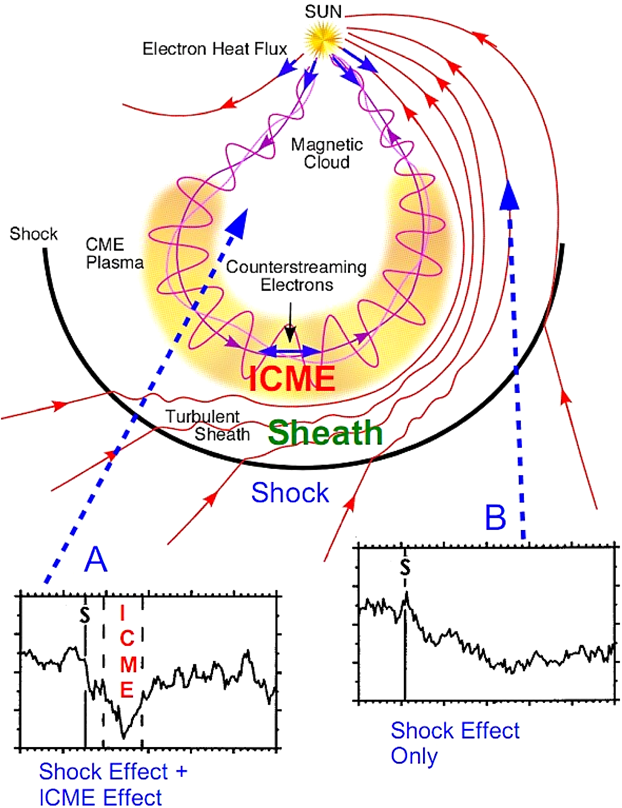
\includegraphics[width=0.6\textwidth]{images/richardson_cane_2011_icme.png}
	\caption[Illustration of ICMEs and Forbush decreases]{Illustration of an \ac{ICME} that drives a shock and the \acp{FD} it causes at two locations A and B (marked by the blue dashed arrows). A classical two-step Forbush decrease is seen at location A, where both the shock/sheath and the magnetic cloud pass. A location B, only a single-step Forbush decrease is observed because only the shock is seen here. The red and pink arrows indicate selected magnetic field lines. Source: \citet[Figure 1]{Richardson-Cane-2011}, reprinted by permission from Springer Nature.}
	\label{fig:richardsoncane-cme}
\end{figure}
Typical amplitudes of \acp{FD} can range from a few percent up to more than \SI{10}{\percent} depending on the event, but this varies significantly depending on which \ac{GCR} energies are observed: Lower energy particles are modulated more easily and thus show larger \acp{FD} \citep[e.g.][]{Lockwood1971,Lockwood1991}.

Over time, multiple models have been proposed to describe \acp{FD} caused by different magnetic structures, and these are often based on a diffusion equation. For example, the \acl{PDB}\acused{PDB} model \citep[\acs{PDB},][]{Wibberenz-1998} can be used to describe a shock that acts as a barrier through which \acp{GCR} cannot diffuse as easily as in the ambient solar wind. This creates a ``shadow'' within and behind the shock in which the \ac{GCR} intensity is decreased.
The \ac{ForbMod} developed by \citet{Dumbovic2018-ForbMod} builds on top of this approach to model \acp{FD} caused by flux rope \acp{CME} by combining the diffusion process with an expanding cylindrical flux rope structure. In this case, the flux rope initially does not contain any \acp{GCR} close to the Sun, and they can gradually diffuse into it (perpendicular to the magnetic field) over time. The time evolution of the \ac{GCR} density within the flux rope is determined by the interplay of its self-similar expansion and the efficiency of the \ac{GCR} diffusion. In a following article \citep{Dumbovic-2020-ForbMod} the model was combined with empirical equations for the energy dependence of the diffusion process, so that \acp{FD} measured using different instruments can be modeled by taking into account their response functions. \ac{ForbMod} has been applied in two of the publications included in this PhD thesis \citep{Forstner-2020,Forstner-2021-SolO} and further details about its derivation are given in these publications.

\section{Motivation}
\label{sec:motivation}

To better understand the propagation of \acp{ICME} in the heliosphere, their radial evolution and impacts on Earth, it is essential to make measurements not only in situ at Earth, but from as many locations as possible, to be able to validate and calibrate modeling approaches and thus improve our forecasting capabilities. This includes both in situ measurements at different locations on the \ac{ICME}'s trajectory, e.g. as an upstream monitor on the Sun-Earth line to give early warning of an approaching \ac{ICME}, as well as remote sensing observations from the side to better understand the global \ac{CME} characteristics. Measurements at other locations also become increasingly relevant not only for Earth, but also for the large amount of operating and planned space missions (including e.g. human spaceflight to Mars in the next decades), which are in need of space weather forecasting as well for ensuring the safety of spacecraft and astronauts.

While some spacecraft with appropriate plasma and magnetic field measurements for these purposes are already available, it is also sensible to introduce \acp{FD} into the framework of space weather observations, as some missions only carry particle detectors or provide other data only in limited form. For example, the \ac{RAD} instrument on the \ac{MSL} mission, which will be introduced in \autoref{sec:mslrad}, is the only instrument that provides continuous measurements of space weather at Mars through its \ac{FD} observations --- other missions such as Mars Express (2003) and \acl{MAVEN}\acused{MAVEN} (\acs{MAVEN}, 2014) carry some plasma and/or magnetic field instruments, but only have limited coverage as their orbits cross below Mars's bow shock so that the upstream solar wind cannot be observed all the time. This thesis will present the first systematical studies of Forbush decreases caused by \acp{ICME} at Mars using the \ac{RAD} cosmic ray data and use the measured \ac{CME} arrival times as well as remote sensing data from \ac{STEREO}-\ac{HI} to validate different modeling approaches. Furthermore, it will be explored whether it is possible to derive more information about the \ac{CME} evolution than just the arrival times from the \ac{FD} observations by applying reverse modeling approaches, and case studies of some notable space weather events will be conducted.

In \autoref{chp:instruments}, a detailed overview of the most important instruments employed in these studies and their data products will be given. The following chapters present several peer-reviewed publications that study \ac{ICME} arrival times at \SI{1}{\AU} and Mars using \acp{FD} and remote sensing observations (\autoref{chp:arrival_times}), additional properties of \acp{FD} at Earth and Mars and their implications for \ac{CME} radial evolution (\autoref{chp:fd_properties}) as well as case studies of a major \ac{SEP} event at Mars that was associated with multiple \acp{ICME} (\autoref{chp:september_event}) and of the first \ac{ICME} and the corresponding \ac{FD} observed at the Solar Orbiter spacecraft (\autoref{chp:solo}). Three appendices follow, which describe certain technical aspects of these studies in more detail, such as the derivation of response functions for the \ac{HET} onboard Solar Orbiter (\autoref{chp:HETSimulation}) and the development of a new software implementation of the \ac{GCS} model for the reconstruction of \acp{CME} in remote sensing observations (\autoref{chp:GCS_Python}). Finally, \autoref{chp:Publicationlist} presents a list of all publications that I have contributed to, including those that are not included within this PhD thesis as they do not directly fit into the logical flow.


\chapter{Instrumentation}
\label{chp:instruments}

\section{Chang\'E-4 and Lunar Lander Neutron and Dosimetry Experiment}
\label{sec:change_4_LND}

\begin{figure}
    \centering
    \includegraphics[width = 0.4\textwidth]{images/LND_2018-11-13.JPG}

    \caption{The photographs of LND instrument, including the sensor head (SH, front), and electronics box (EB, rear), and 1-meters data and powver harness that connects the SH and EB. The figure was from \cite{Wimmer-2020-LND} which is actually the flight spare model of LND and wass token on 2018-11-23 for the instrument paper}
    \label{Fig:LND_instrument}
\end{figure}

\begin{figure}
    \centering
    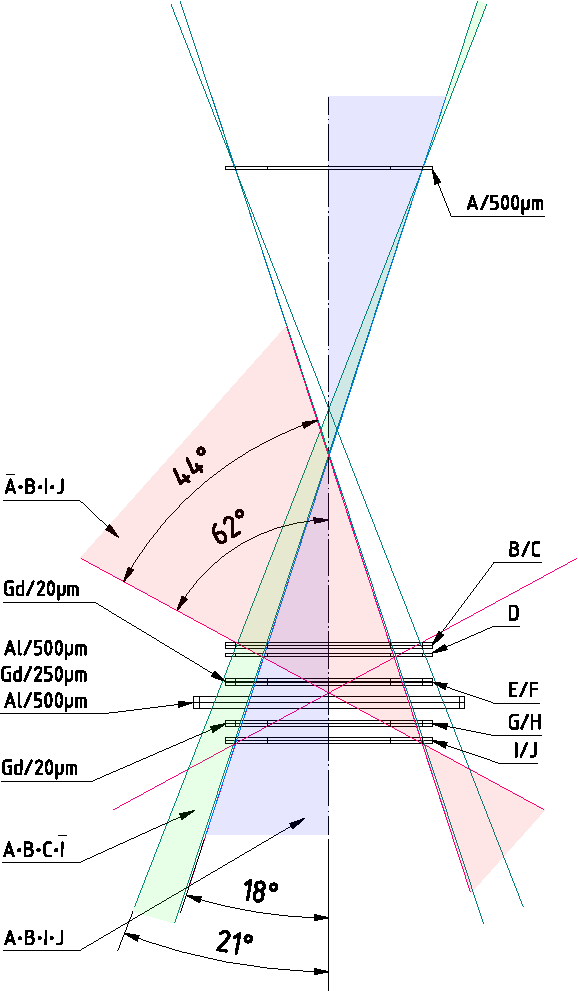
\includegraphics[width = 0.4\textwidth]{images/change4_lnd-c9_trigger-cones-colored.pdf}
    \caption{The skeptical view of the inner structure of the sensor head. Ten 500 $\mu$m silicon \acs{SSD} are assembly in order from A to J. The figure was from \cite{Wimmer-2020-LND}. More detailes could be found in the instrument paper.}
\end{figure}
Chang'E-4 is a chinese lunar exploration mission to the lunar far-side surface, which is also the first human mission sofely landed on the lunar far-side surface. The whole mission consists of a lander, a rover (Yutu-2, citaion) and a relay sattellite (Queqiao, citaion) which is working in the lunar orbit and responsible for the communication between the lunar far-side surface and the ground. The mission was launched on December 7, 2018 and successfully landed on January 3, 2019 in the Von K\`arm\`an crater near the south pole of Moon. 

There four 


including 4 international     al payloads and 4 domestic payloads.
Environment, 
Up to now.

As one of the four internation payload, LND is designed by  Kiel University
Which is a  instrument 
Aim at 
The main scientific objects of LND, as indicated in the instrument paper, are the following:
\begin{itemize}
    \item Dosimetry for human exploration of the Moon
    \item Contribution to the heliospheric science
\end{itemize}
And LND also has two technological demonstration objects which are \textit{Determine the subsurface water content in the South-Pole Aitken Basin} and \textit{Determine the FeO content in the South-Pole Aitken Basin} 
To achieve the above scientific objects, LND measure and provide the data products including up to 1-minute charged and neutral particle dose rate measured in Si, up to 1 minute cadence LET spectra, 1 minute neutral particle deposition energy spectra, 10 minute count rates of thermal neutrons and high time resolution (1-min, 10-min) flux and high energy resolution charged particle spectra including the electron and ions from proton to iron.


LND only working on the local day time of lunar farside. One of major challenge of LND on the lunar far-side surface is the 
The easiest way to check whether LND is working or not is looking up during night, if you see a ? moon, which indicates that moon is moving our of the earth's shawdown and the farside is facing the sun. Once the light is arriving at the lander, the system will be waken up and start to work. So is LND and other instruments.

Up to May 2023, LND has been working on the lunar far-side surface for more than 4 years (more then 50 Lunar days), already exceeding its designed life time. 

LND was switch off or switch on for a short period on the 6th, 44th, 45th lunar days, due to the special operations of lander and the extre movement from the ground. Up to May 2023, when the thesis finished, we have received the 46 lunar day data from January 2019 to the end of November 2022. The more data is coming. 
The data is officially publishing in the Lunar and Planetary Data release system \url{moon.bao.ac.cn}. An alternative way to download the data is from the PDS \url{https://pds.nasa.gov/}. The data is also available in the \ac{PSA} \url{https://psa.esac.esa.int/psa/}.

After LND delivered and launched, we implement several configuration changes and upload together 14 extra commands to fix the issues including the design issue and the malfunction issue. The design issue is due to the bugs in the processing software causing the wrong usage of the channels. The affection on the data products is minor. However, the major change of the data products are caused by the sky rocket of the noise level in certain channels. The reason for the noise issue is due to the unproper operation in the ground. On the 3rd and 4th lunar day, LND was switched off but kept the LND lid open until LND was switch shortly after. The immediately consequence of such operation is the dramastically drop of the temperature on the detector. Such a change is unrecoveryable, even if the temperature is back to normal.

To mitigating the impact of the noise issue and its influence on the data products, we implement several changes including raise the threshold of the noise detector, disable A2 channels which larger affect the LET spectra and hardly fixed by raising the threshold. No doubt, the consequence of such changes is obviouse. For instance, we lose the measurement of minimum ioninzing particle after the increment of the threshold of I detector, and the geometry factor of LET spectra and penetrating particle are dramatically reduced since we disable A outer channels. 

The details of the configuration changes and affections are given in the Appendix of chapter \ref{} and the corresponding change of the original code in the LND data processing software is given in the appendix ( if you have time to do it)

As we listed before, a major 

\subsection{The charged particle telescope of LND}








Most importantly LND as the charged particle telescope:

The measurment principle





\subsection{The other opportunity of the LND}


During the first half year of Chang'e-4 mission, the sun had a extremely quite phase and the solar activities reached the minimum level as indicated by the monthly averaged sunspot number which is nearly zero according to the observation from *****. Furthmmore, almost no SEP events happened during this period. 

On the other side, the crucial environment on the lunar far-side surface is a big challenge for the LND to work properly. The
The LND is designed to work in the temperature range of -40 to 60 degree, but the temperature on the lunar surface could be as low as -180 degree during the night.
In order to protect the detectors from the frozen temperature, the LND is only allowed to work during the day time after the lander is raised by the light of the sun.
During night, the RTG and RHU heater will keep the Lander and other scientific payload warm. 
Since LND only work 1\/3 of the time, the chance that LND encounter a SEP event during the solar minimum is even lower.

However, the LND is still lucky enough detecting several SEP events during the first half of 2019. 
On May 2019, two SEP events arrived on the lunar surface and 





\section{Solar orbiter and High energy telescope}

Launched on Feb 10, 2020, \acl{SolO}\acused{SolO} missions [citation] is an international mission cooperated between \ac{ESA} and \ac{NASA}. The aim of this mission is to understand the sun and how it control the so-called helisphere. As indicated in solo mission paper, the following scientifice questions will be answered and further studies:
\begin{itemize}
	\item 1
	\item 2
	\item 3
\end{itemize}
After finishing the cuise phase which started at June 14, 2020, currently, \ac{SolO} is operating as planned in the nominla mission phase since Nov 26, 2021.
The \ac{SolO} has a special designed elliptic helioscentric orbit with the closest perihelion of 0.29 AU (about 42$\times10^6$ km) in the whole mission. Using several gravity assistance during the venus flyby and earth flyby, the orbit of SolO will gradually tilt away from the ecliptic plane, in the end is 24 degrees above the Sun's equator.

Up to May 2023, when this thesis is drafted, \ac{SolO} is still following an elliptical orbit around the sun, with a maximum solar latitude of 8.66 degrees. \ac{SolO} has finished 5 perihelions with closest distance of 0.292 AU on Sep 3, 2022, and is starting its 6th orbit, moving on the way away the Sun. Three time Venus flyby happened on Dec 27, 2020,  Aug 9, 2021 and Sep 4, 2022. The Earth GAM happend on Now 27, 2021.

The above mentioned solo tragjectory information is taken from the \hyperlink{https://issues.cosmos.esa.int/solarorbiterwiki/display/SOSP/Trajectory+Overview+-+10+February+2020+Launch}{Solar orbiter Consolidated Report on Mission analysis}

Benefit from the special position of \ac{SolO} during this trip, the multiple scientific instrument onboard the \ac{SolO} coudl furtherly advanced the studies  in relative field and certain topic, for instance, remote- sensing [?], solar wind [?], SEP [?], GCR [?].

EPD [citation here]is one of such scientific payload suite onboard solo, aiming at the charge particles with energy spans over a large scale from few kev to few GeV,In this larger energy range, all the plasma population including lower energy solar wind,  $\sim$ kev suprathermal particle, high energy SEP, ACR and GCR are measured and studies.
EPD consists of four instruments, \ac{SIS}, is a time-of-flight mass spectrometer that measures ion composition from  $\sim$ 0.1 - few MeV
10 MeV nucleon$^{-1}$ designed by JPL; \ac{STEP}, is ? that measures what?;  \ac{EPT} is ? and measure ? and \ac{HET}, is what and measure what
Apart from SIS, all other instrument are design by Kiel group.
Those four instruments are assembly on the SolO as the Fig.{}explain the instrument together image. The energy coverage of those four instruments are shown in Fig.{EPD energy range}.

In the following section, we briefly introduce some details of the \ac{HET}, which is the mainly used in our study.

Overview
\subsection{High energy telescope}

The high energy telescopes (HET), as one of the scientific payload of The Energetic Particle Detector (EPD) \cite{EPD_instrument} on the Solar Orbiter, are designed to measure the high energetic particles and cover the higher end of the EPD energy range. The typical particles that HET measures include $\sim$ MeV electrons [citaion] and tens of MeV to few GeV positively charged particles like, protons, helium-4 and its isotope Helium-3, carbon, oxygen, nitrogen, and even heavy elements iron. 

Two HET units, HET1 and HET2, are equiped on the \ac{SolO}. They are specially mounted on two perpendicular direcitons, sun-asun (ecliptic) and south-north (polar), providing the angle information of particles in the interplanetary space[citatoin]. Such measurements are especially useful during the SEP event because the pitch angle  distribution of energetic paricle in the magnetic field is an important paramter to understand the transportation of particle [citaion, find precious words]. 

Each HET is a double-ended telescope which consists of four 300 $\mu$m silicon solid-state (SSD) detectors stacks, with two in each side (A1, B1 in the front side and A2, B2 in the back side), and a 2 cm thick $Bi_{4}Ge_{3}O_{12}$ (BGO) scintillator, in the center. The inner structure of the HET sensor head is given in Fig.\ref{fig:HET-sensor-head}. HET use the dE/dX - E technique to discriminates different particle species of different energy, including electron, proton, helium-4, and heavy ions like carbon, nitrogen, oxygen, and iron.  ( to expand and more details)



\begin{figure}
    \centering
    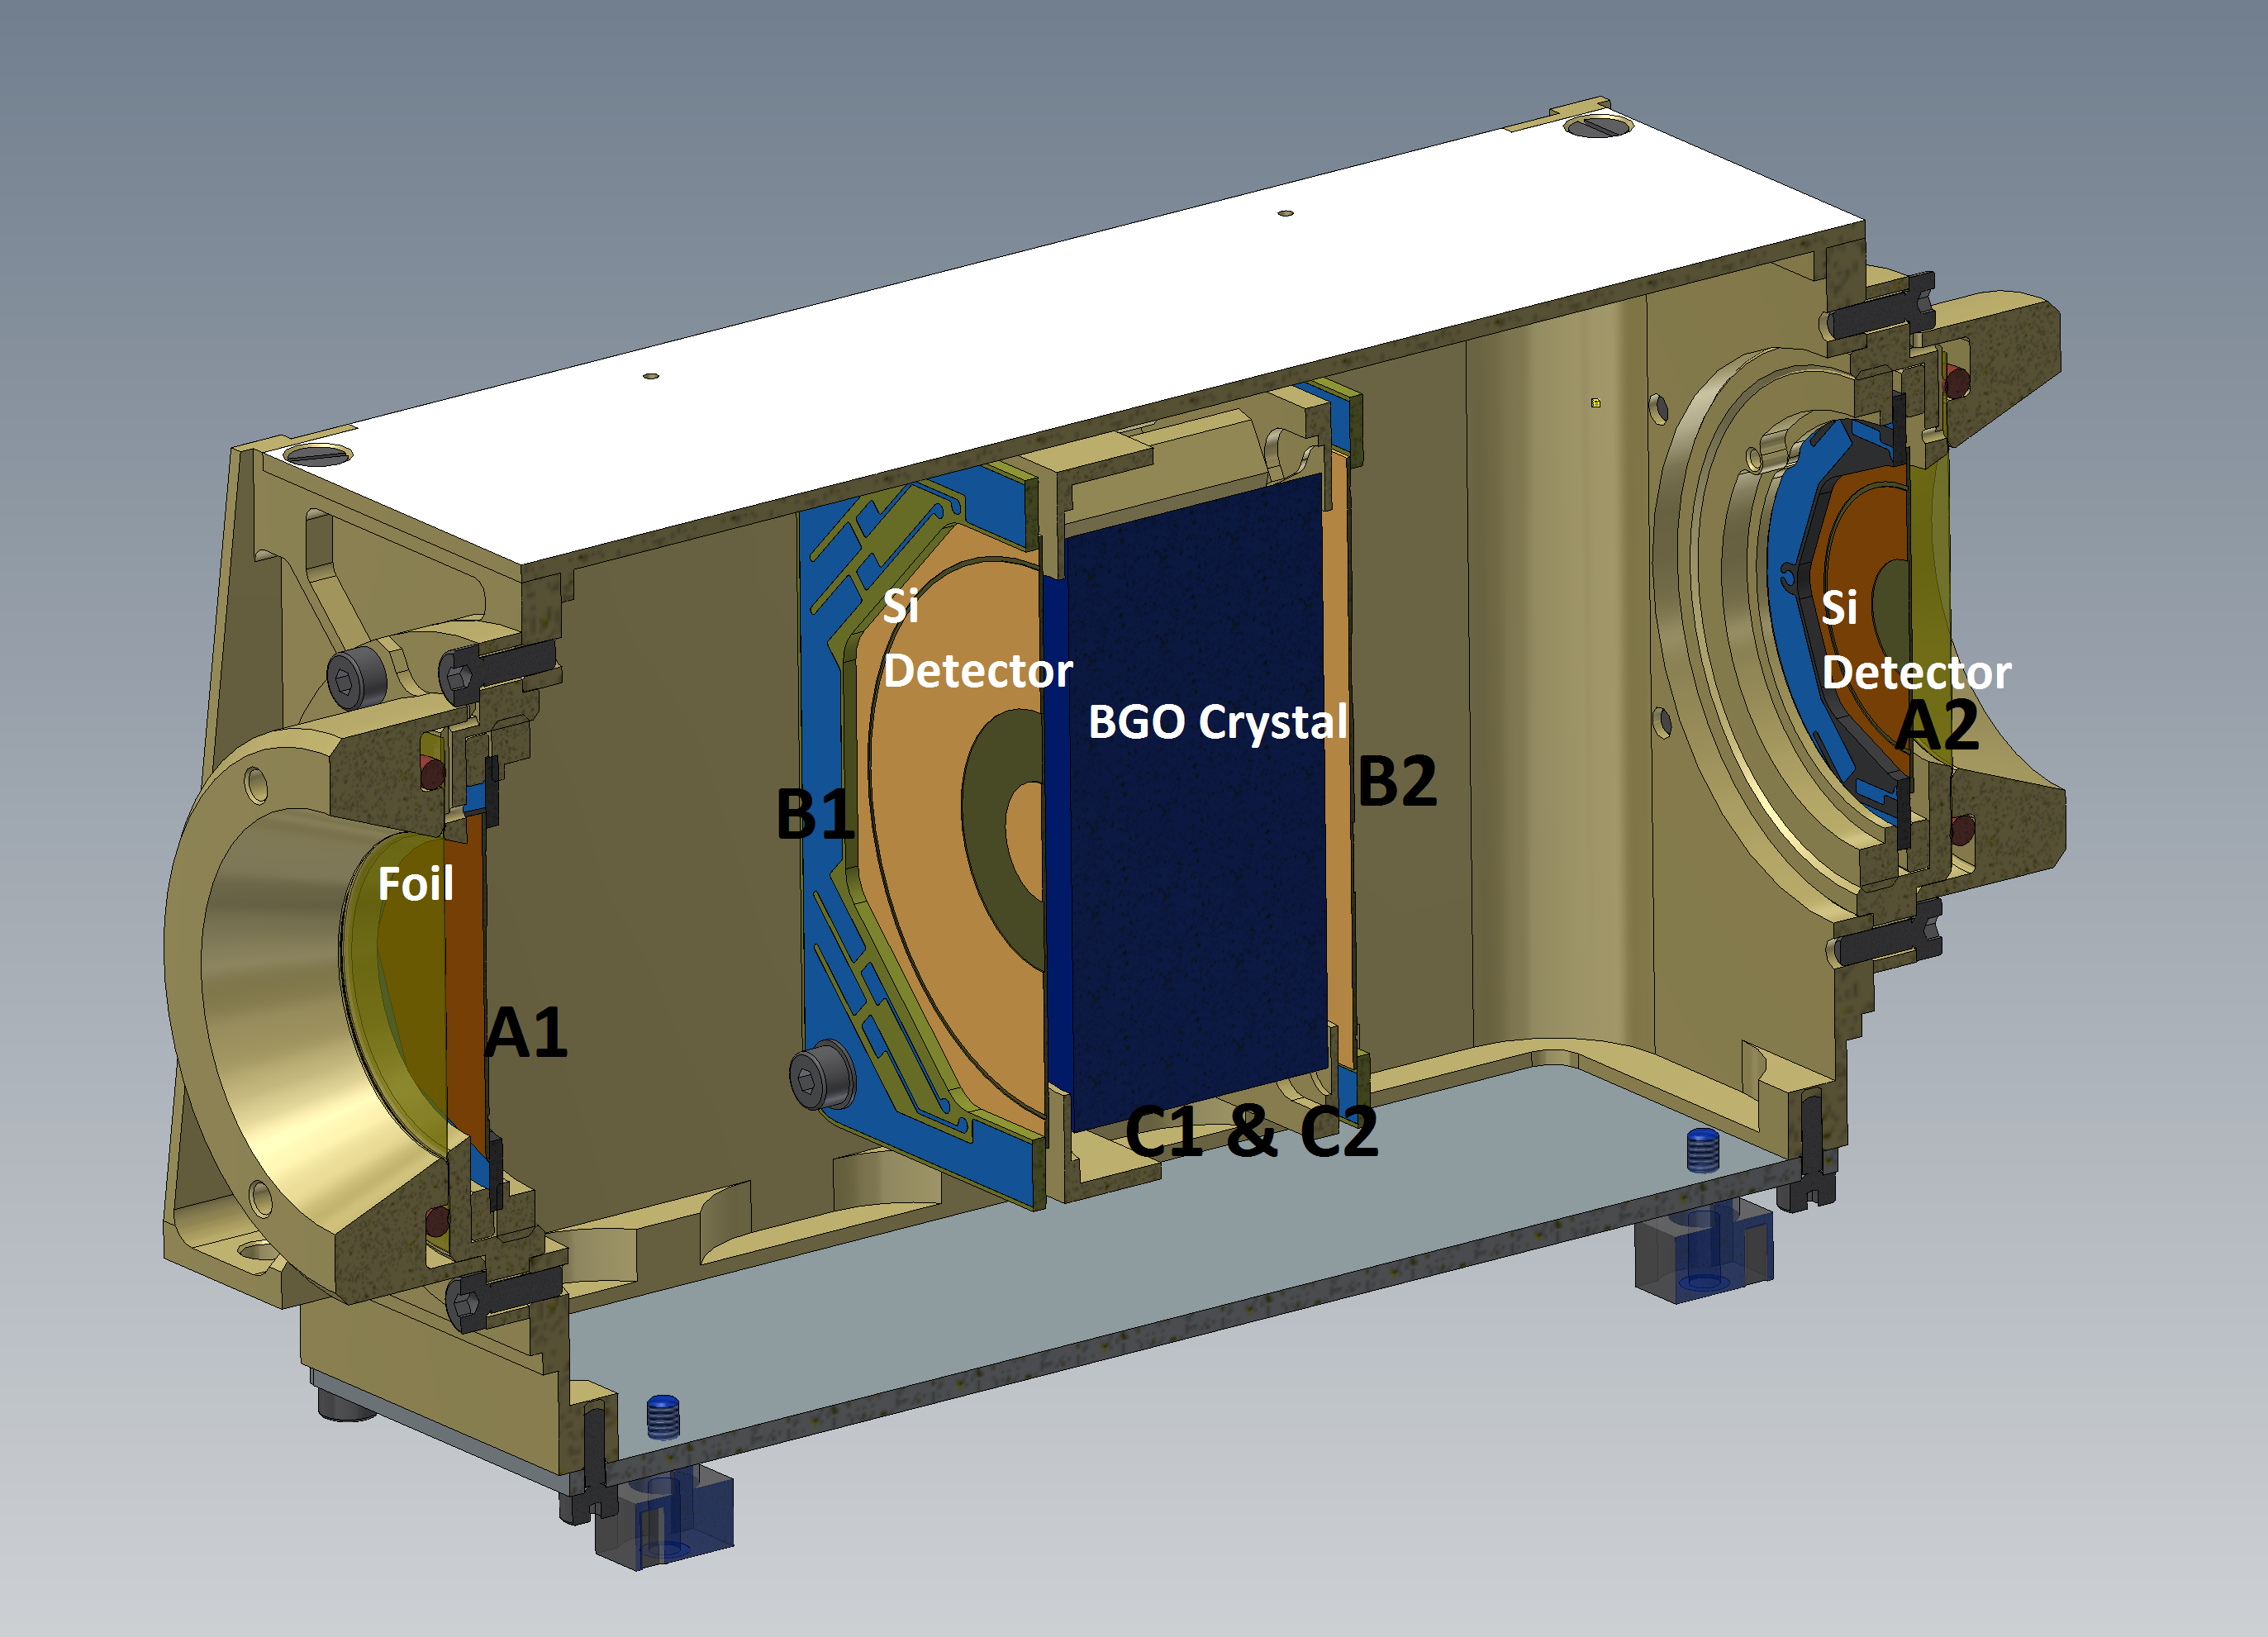
\includegraphics[width = 0.6\textwidth]{images/het.png}
    \caption{The sensor head o}
    \label{fig:HET-sensor-head}
\end{figure}



As given in Table 22 of \cite{EPD instruemnt},the nominal data products of HET include ABnC (6.5 - 9.5 Me\/nuc), ABC ($\sim$10 - $\sim$ 100 MeV/nuc) and penetrating (above 100 MeV/nuc). The energy range in the bracket are the designed energy range of helium-4 measurement by HET. In this study, we use the data products that measure helium stopping in inner C detector i.e. the ABC coincidence and we specially use the energy between 10 - 50 MeV\/nuc, because this is exactly the energy region where ACR helium dominate and the data product of SOHO\/EPHIN exaclty cover this energy region which we introduce in the following section. We will calculate the ratio of flux between HET and EPHIN. 
Besides, the lowest energy channels of ABnC coincidence have unsolved calibration issue and the measurement of remain channels are constrained by their counting statistics which result in a relatively larger uncertainties.



The nominal scientific data products of HET are designed to study SEP events of higher intensity by limiting the FOV and using coincidence measurements to discriminate species and achieve better energy resolution. However such data products are not optimal for the analysis that requires both time resolution and larger counting statistc, for instance to determine the SEP events period.    Alternatively, single detector count rates without any coincidence conditions which is one kind of housekeeping data, could provide the possibility to achieve better counting statistic. Von forstner et al 2021 use the single C counter to study the temporal varitation of the forbush decrease and Allen et al 2021 confirmed the drop out of C counter rate during the first venus flyby is due to the VENUS blockage on the HET FOV.

Similar with the single detector count rate, in the study, we introduce \textit{any(a1, b1)} which is a level-2 trigger of HET to determine the SEP period. \textit{a1} and \textit{b1} represent the front two SSDs of HET sensor head. This level-2 trigger counts all the particles that have energy above the threshold of detector A or detector B, which is 50 keV in the nominal mode [citaion effman thesis]. Since no obstacles in front of A detector, both electron and protons with small energys could be counted in this trigger and not a single SEP event will be missed in the change of time series of \textit{any(a1,b1)}, even though sometimes no corresponding helium-4 change reflected in the flux higher energy channels.

For more details of the inner structure and parameter of the HET, and the most update status of HET, one could refer to \citep{2020AA_EPD} and \citep{wimmer2021AA}.

% Built in a cooperation between the University of Kiel and Southwest Research Institute, the \acl{RAD}\acused{RAD} \citep[\acs{RAD},][]{Hassler-2012-MSLRAD} instrument onboard the \acl{MSL}\acused{MSL} \citep[\acs{MSL},][]{Grotzinger-2012} mission provided the first-ever direct radiation measurements on the surface of Mars. It is designed to measure both charged and neutral particles, and calculate particle spectra as well as dosimetric quantities, such as the \ac{TID} rate and \ac{LET} spectra. This aligns with its main science objectives, which include the characterization of energetic particle spectra on the surface of Mars (\acp{GCR} and \acp{SEP}) and the determination of the radiation hazard for past or present life on Mars or for future human Mars missions. Consequently, \ac{RAD} has not only been continuously measuring the radiation environment on the Martian surface since the \textit{Curiosity} rover's landing on August 6, 2012, but has also been active during the most part of its 9-month flight to Mars (the so-called cruise phase) to evaluate the radiation dose that astronauts would be exposed to when traveling to Mars.



% \begin{figure}
% 	\centering
% 	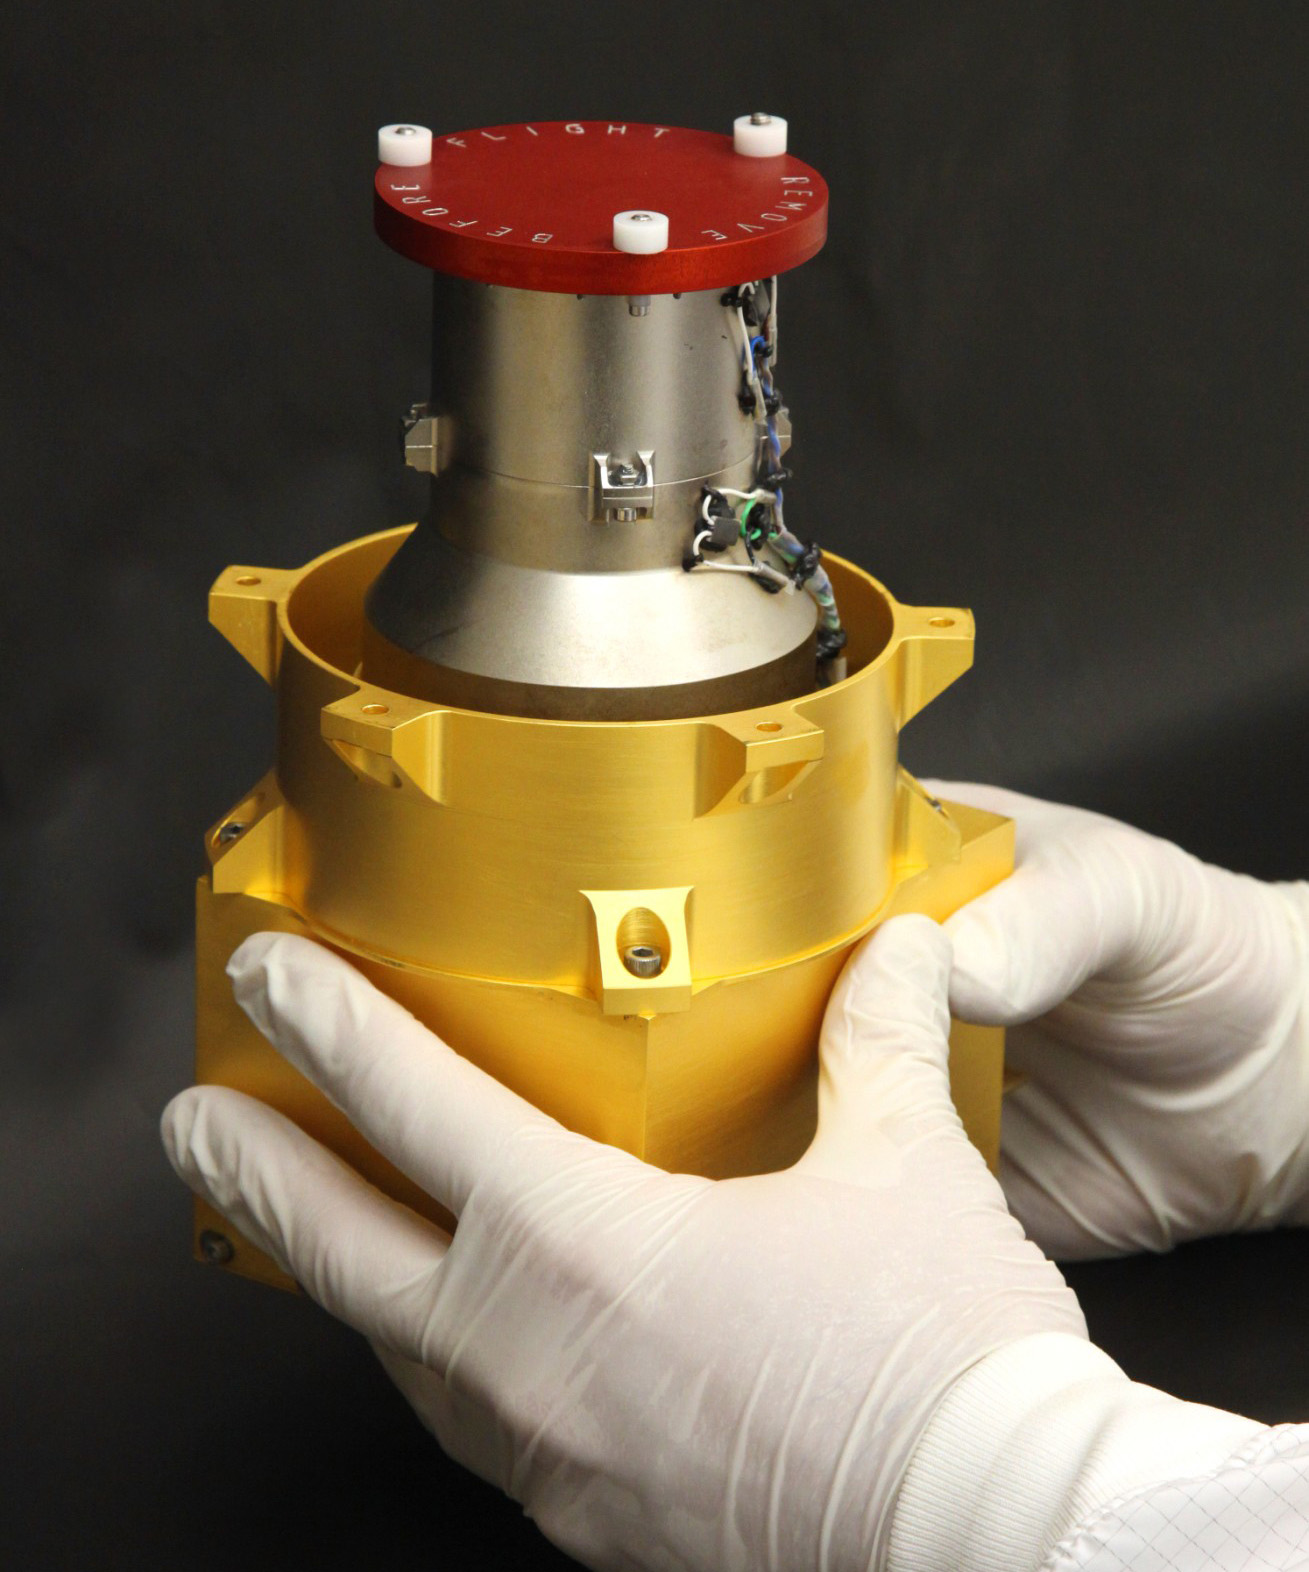
\includegraphics[width=0.4\linewidth]{images/rad}
% 	\caption[Photo of the \acs{RAD} sensor head]{A photo of the \ac{RAD} sensor head before it was mounted on the \ac{MSL} spacecraft. The red protection cap was removed after installation on the rover. Source: NASA/JPL-Caltech/SwRI}
% 	\label{fig:rad-photo}
% \end{figure}

% The \ac{RAD} sensor head (shown in \autoref{fig:rad-photo}) is mounted on the top deck of the rover, pointing along the z axis of RAD, i.e. towards the zenith. It is composed of three hexagonal silicon solid-state detectors (A, B, and C) with a thickness of \SI{300}{\micro\meter} each, mounted in a stack to form a charged particle telescope (\autoref{fig:rad-sensorhead}) with an opening angle of about \SI{60}{\degree}. Each detector is divided into an inner and an outer segment.
% The D detector, a cesium iodide (CsI) scintillator in the shape of a truncated hexagonal pyramid, is situated directly below the charged particle telescope. Its shape is designed to align with the inner segment of C and follows the opening angle of the charged particle telescope (shown with dashed lines in \autoref{fig:rad-sensorhead}). The E detector, a plastic scintillator which is located below D, is mainly responsible for neutral particle detection. D and E are surrounded by another plastic scintillator (F), which is used as an anticoincidence shield to reject ions that enter D or E from the sides.

% \begin{figure}
% 	\centering
% 	%\documentclass{standalone}
%\usepackage{tikz}
%\usepackage{amsmath}

%\usetikzlibrary{calc}
%\usetikzlibrary{decorations.pathmorphing}

%\definecolor{light-gray}{gray}{0.9}

%\begin{document}
\begin{tikzpicture}[scale=0.8]
    \tikzset{%
        add/.style args={#1 and #2}{
            to path={%
                ($(\tikztostart)!-#1!(\tikztotarget)$)--($(\tikztotarget)!-#2!(\tikztostart)$)%
                \tikztonodes},add/.default={.2 and .2}}
    }  
    
    \def\bottomwidth{3.25}
    \def\midwidth{1.8}
    \def\topwidth{1.65}
    \def\bottomheight{2.5}
    \def\midheight{4.375}
    \def\Fthickness{1}
    \def\Sithickness{0.1}
    \def\BCdistance{0.15}
    \def\topheight{8.375}
    
    % FOV
    \draw[add=0 and 0.3, dashed] (\midwidth - \Fthickness, \midheight) to (-\topwidth, \topheight);
    \draw[add=0 and 0.3, dashed] (-\midwidth + \Fthickness, \midheight) to (\topwidth, \topheight);

    % A
    \draw[fill=light-gray] (-\topwidth, \topheight - \Sithickness) rectangle (\topwidth, \topheight);
    \draw (-\midwidth + \Fthickness, \topheight - \Sithickness) --  (-\midwidth + \Fthickness, \topheight);
    \draw (-\midwidth + \Fthickness, \topheight - \Sithickness) --  (-\midwidth + \Fthickness, \topheight);
    \draw (\midwidth - \Fthickness, \topheight - \Sithickness) --  (\midwidth - \Fthickness, \topheight);
    \draw (\midwidth - \Fthickness, \topheight - \Sithickness) --  (\midwidth - \Fthickness, \topheight);
    \draw[latex-] (-\topwidth, \topheight - \Sithickness / 2) -- (-\topwidth - 0.5, \topheight - \Sithickness / 2) node[left] {A};
    
    % B
    \draw[fill=light-gray] (-\topwidth, \midheight + \BCdistance) rectangle (\topwidth, \midheight + \BCdistance + \Sithickness);
    \draw (-\midwidth + \Fthickness, \midheight + \BCdistance) --  (-\midwidth + \Fthickness, \midheight + \BCdistance + \Sithickness);
    \draw (-\midwidth + \Fthickness, \midheight + \BCdistance) --  (-\midwidth + \Fthickness, \midheight + \BCdistance + \Sithickness);
    \draw (\midwidth - \Fthickness, \midheight + \BCdistance) --  (\midwidth - \Fthickness, \midheight + \BCdistance + \Sithickness);
    \draw (\midwidth - \Fthickness, \midheight + \BCdistance) --  (\midwidth - \Fthickness, \midheight + \BCdistance + \Sithickness);
    \draw[latex-] (-\topwidth, \midheight + \BCdistance + \Sithickness / 2) -- (-\topwidth - 0.5, \midheight + \BCdistance + \Sithickness / 2 + 0.3) node[left] {B};
    
    % C
    \draw[fill=light-gray] (-\topwidth, \midheight) rectangle (\topwidth, \midheight + \Sithickness);
    \draw (-\midwidth + \Fthickness, \midheight) --  (-\midwidth + \Fthickness, \midheight + \Sithickness);
    \draw (-\midwidth + \Fthickness, \midheight) --  (-\midwidth + \Fthickness, \midheight + \Sithickness);
    \draw (\midwidth - \Fthickness, \midheight) --  (\midwidth - \Fthickness, \midheight + \Sithickness);
    \draw (\midwidth - \Fthickness, \midheight) --  (\midwidth - \Fthickness, \midheight + \Sithickness);
    \draw[latex-] (-\topwidth, \midheight + \Sithickness / 2) -- (-\topwidth - 0.5, \midheight + \Sithickness / 2) node[left] {C};
    
    % border of ABC
    \draw (-\topwidth, \midheight) -- (-\topwidth, \topheight);
    \draw (\topwidth, \midheight) -- (\topwidth, \topheight);
    
    % D
    \draw[fill=light-gray] (\bottomwidth - \Fthickness, \bottomheight) --  (-\bottomwidth + \Fthickness, \bottomheight) -- (-\midwidth + \Fthickness, \midheight) -- (\midwidth - \Fthickness, \midheight) -- (\bottomwidth - \Fthickness, \bottomheight);   
    \node at (0, {\bottomheight + (\midheight - \bottomheight) / 2}) {D};   
    
    % E
    \draw[fill=green!50] (\bottomwidth - \Fthickness, \bottomheight) -- (\bottomwidth - \Fthickness, \Fthickness) --
    (-\bottomwidth + \Fthickness, \Fthickness) --  (-\bottomwidth + \Fthickness, \bottomheight) -- (\bottomwidth - \Fthickness, \bottomheight);  
    \node at (0, {\Fthickness + (\bottomheight - \Fthickness) * 0.4}) {E};   
    
    % F
    \draw[fill=yellow] (-\bottomwidth, 0) -- (\bottomwidth, 0) -- (\bottomwidth, \bottomheight) -- (\midwidth, \midheight) --
    (\midwidth - \Fthickness, \midheight) -- (\bottomwidth - \Fthickness, \bottomheight) -- (\bottomwidth - \Fthickness, \Fthickness) --
    (-\bottomwidth + \Fthickness, \Fthickness) --  (-\bottomwidth + \Fthickness, \bottomheight) -- (-\midwidth + \Fthickness, \midheight) --
    (-\midwidth, \midheight) -- (-\bottomwidth, \bottomheight) -- (-\bottomwidth, 0);     
    \node at (0, \Fthickness / 2) {F};
    
    % trajectories of ions
    \draw[thick, green, -latex] (-\topwidth*0.7, \topheight*1.15) node[above, align=center] {\small Ion\\ \small (accepted)}
     -- ({-(\midwidth - \Fthickness) * 0.5}, \midheight + \Sithickness / 2);
    \draw[thick, green, -latex] (\topwidth*0.65, \topheight*1.15) node[above, align=center] {\small Ion\\ \small (accepted)}
     -- ({-(\midwidth - \Fthickness) * 0.5}, {\bottomheight +  (\midheight - \bottomheight) / 2});
    \draw[thick, red, -latex] (0, \topheight*1.3) node[above, align=center] {\small Ion\\ \small (rejected)}
     -- (0, \topheight - \Sithickness / 2);
    \draw[thick, red, -latex] (\bottomwidth, \midheight) node[above right, align=center] {\small Ion\\ \small (rejected)}
    -- (\bottomwidth * 0.4, {\bottomheight + (\midheight - \bottomheight) * 0.2});
    
    % trajectory of neutron
    \draw[thick, gray, -latex] (-\bottomwidth*0.3, -0.5) node[below] {\small Neutron (accepted)}
    -- (-\bottomwidth*0.3, {\Fthickness + \bottomheight * 0.2});
    \draw[thick, gray, -latex]  (-\bottomwidth*0.3, {\Fthickness + \bottomheight * 0.2}) -- (-\bottomwidth * 1.1, \bottomheight * 1.3);
    \draw[thick, blue, -latex]  (-\bottomwidth*0.3, {\Fthickness + \bottomheight * 0.2}) -- (0, \bottomheight * 1.1) node[midway, right, xshift=1mm] {\small Recoil proton};
    
    % trajectory of gamma
    \draw[thick, gray, decorate, decoration=snake] (-\bottomwidth*1.2, \bottomheight * 0.8) node[below, align=center, xshift=-4mm] {\small $\gamma$-ray\\ \small (accepted)} -- (-\bottomwidth * 0.3, \bottomheight * 1.4);
    \draw[thick, gray, -latex] (-\bottomwidth * 0.3, \bottomheight * 1.4) -- ++ (\bottomwidth * 0.03, \bottomheight * 0.02);
    
\end{tikzpicture}
%\end{document}
% 	\caption[Schematic diagram of the \acs{RAD} sensor head]{Schematic diagram of the \ac{RAD} sensor head. Red, green, blue and gray arrows show possible trajectories of charged and neutral particles through the detectors. Based on      \textcite{Hassler-2012-MSLRAD}, Fig. 7b}
% 	\label{fig:rad-sensorhead}
% \end{figure}

% For the detection of charged particles, \ac{RAD} requires an energy deposit in at least the A and B detector, which sets the lower limit for the particle's kinetic energy to e.g. \SI{6}{\mega\electronvolt} for protons. Higher energy charged particles penetrate the B detector and stop in C, D, or E, where the high stopping power of the D detector allows for a large energy range, e.g. up to \SI{95}{\mega\electronvolt} for stopping protons. For stopping charged particles, the charge and the total kinetic energy can be determined from the two measured quantities, the total deposited energy $E$ in all triggered detectors and the \ac{LET} (deposited energy per path length) $\dd E/\dd x$ in one of the detectors. This common principle is called the $\dd E/\dd x$-$E$ method and has been in use in numerous instruments since the IMP-\liningnums{1} mission in the 1960s \citep{McDonald-1964}.

% Higher energy charged particles, which penetrate the whole \ac{RAD} sensor, cannot be analyzed using this technique, as the total energy $E$ is not measured directly in this case. Up to a few hundred \si{\mega\electronvolt} per nucleon, particles can still be partially analyzed as their \ac{LET} is slightly different at the top and bottom ends of the telescope. In this case, the \ac{LET} ratio between the top and bottom can be used to infer the approximate kinetic energy of the incoming particle. For even higher energy particles, the so-called \acp{MIP}, there is no significant change in the \ac{LET}, so only the charge and \ac{LET} can be determined, but not the primary energy.

% The D and E detectors are both, to different degrees, also sensitive to neutral particles. Being a CsI scintillator, D can detect secondary electrons produced by $\gamma$-rays effectively, while neutrons hitting E can interact with the hydrogen atoms in the plastic to produce recoil protons. An inversion method that takes all these interaction processes into account is then used to derive neutral particle spectra \citep{Koehler-2011}.

% Being an instrument with a rather low mass (\SI{1.6}{\kilogram}) and volume, the observation of short-term and low-amplitude \ac{GCR} variations such as Forbush decreases with \ac{RAD} is only possible when measuring particles that enter the sensor head from all directions, as the restricted opening angle of the charged particle telescope decreases the count rate too much. In this case, the dose rate data products of \ac{RAD} can be used, which are available for the B and E detectors. The E detector is best suited for this purpose due to its larger volume and therefore better statistics.
% The dose in a detector is calculated as
% \begin{equation}
% D = \frac{E_\text{dep}}{m},
% \end{equation}
% i.e. the total energy deposited in the detector divided by its mass, and typically given in units of $\si{\gray} = \si{\joule\per\kilogram}$. The dose rate is its time derivative, so it is given in \si{\gray\per\second} (or \si{\micro\gray\per\day}, for the order of magnitude that is typically observed on planets). In comparison to a simple count rate, where each detected particle increases the counter by one, particles stopping in the detector typically contribute more to the dose rate than penetrating particles, as the former deposit all their energy.

% Because \ac{RAD} is located on the surface of Mars, incoming primary \ac{GCR} and \ac{SEP} particles first need to travel through the Martian atmosphere before reaching the \ac{RAD} detectors. In this process, some particles are shielded away, while others can generate secondary particles by interacting with the particles in the atmosphere. Thus, the radiation environment observed by \ac{RAD} is a mix of primary and secondary particles, and \ac{RAD} measurements cannot be directly compared to deep-space detectors without taking into account the atmospheric response functions \citep[see e.g.][]{Guo-2017,Guo-2019}. For example, \ac{SEP} events need a certain minimum energy to be observed on ground, so \ac{RAD} only sees the most intense events as a \ac{GLE}.

% The atmospheric pressure measured by the \ac{REMS} instrument onboard \ac{MSL} shows a significant daily variation of about $\pm\SI{5}{\percent}$ \citep{Haberle-2014} due to the considerable temperature changes between day and night --- for comparison, the diurnal pressure variations on Earth are at least an order of magnitude lower \citep[e.g.][]{LeBlancq-2011}. These pressure variations also influence the \ac{RAD} measurements, as they affect the column mass of the atmosphere above \ac{MSL}, and thus change the amount of secondary particles generated in the atmosphere. A clear correlation between dose rate and pressure was observed by \citet{Guo-2017}. These diurnal variations show amplitudes up to $\sim\SI{2.5}{\percent}$, and this needs to be taken into account when observing short-term variations of the \ac{GCR}, which are typically on a similar order of magnitude. The easiest solution would be to average the dose rate measurements over one solar day (sol) but this would significantly increase the uncertainty for the onset time definition of events such as \acp{FD}. Instead, a spectral notch filter can be applied to the data to filter out the 1 sol frequency and harmonics. This method was described in detail by \citet{Guo-2017-maven} and is also used for most \ac{RAD} data shown within this thesis.
% These considerations about atmospheric effects of course do not apply to the cruise phase data, where \ac{RAD} was relatively lightly shielded by the surrounding \ac{MSL} spacecraft \citep{Zeitlin-2013-cruise,guo2015cruise} and no diurnal effects were observed.

% \section{The Solar Orbiter High Energy Telescope}
% \label{sec:solohet}

% The ESA \acl{SolO}\acused{SolO} spacecraft \citep[\acs{SolO},][]{Mueller-2020-SolO} was launched successfully on February 10, 2020. During its mission, it will travel as close to the Sun as \SI{0.27}{\AU} and provide valuable measurements of all kinds of solar events with its comprehensive remote sensing and in situ instrument suite. The \acl{EPD}\acused{EPD} investigation \citep[\acs{EPD},][]{RodriguezPacheco-2019-EPD} onboard \ac{SolO}, a collaboration of the University of Kiel, the University of Alcalá and the Johns Hopkins University APL, is comprised of four instruments, covering the whole energetic particle spectrum from a few \si{\kilo\electronvolt} up to several hundreds of \si{\mega\electronvolt} (\autoref{fig:epd_energy_ranges}).
% \begin{figure}
% 	\centering
% 	%\documentclass{standalone}
%\usepackage[dvipsnames]{xcolor}
%\usepackage{tikz}
%\usepackage{amsmath}
%\usepackage{siunitx}
%\usepackage{pgfplots}

%\usetikzlibrary{calc}
%\usetikzlibrary{decorations.pathmorphing}

%\definecolor{light-gray}{gray}{0.9}

%\definecolor{red}{HTML}{d62728}
%\definecolor{orange}{HTML}{ff7f0e}
%\definecolor{green}{HTML}{2ca02c}
%\definecolor{blue}{HTML}{1f77b4}
%\definecolor{purple}{HTML}{9467bd}
%\definecolor{light-gray}{gray}{0.9}

%\begin{document}
\begin{tikzpicture}
	\def\xmin{0.002}
	\def\xmax{2000}

	% EPT energy ranges, based on calibration as of 2020-10-01
	% ELECTRONS
	\begin{semilogxaxis}[xmin=\xmin, xmax=\xmax, axis x line=middle, hide y axis, ymin=-2,ymax=2,
					 height=2cm, width=10cm,
					 xlabel={$E$ [\si{\mega\electronvolt}]},
					 x label style={at={(axis description cs:0.5,-0.8)},anchor=north},clip=false,
					 log ticks with fixed point, x tick label style={/pgf/number format/1000 sep={}},yshift=0.4cm]
		\fill[blue, opacity=0.5] (axis cs:0.0041, -1) rectangle (axis cs:0.080, 1);
		\fill[orange, opacity=0.5] (axis cs:0.031, -1) rectangle (axis cs:0.47, 1);
		\fill[green, opacity=0.5] (axis cs:0.45, -1) rectangle (axis cs:18.8, 1);
		\node[left] at (axis cs:\xmin, 0) {$e$};
	\end{semilogxaxis}
	
	% PROTONS
	\begin{semilogxaxis}[xmin=\xmin, xmax=\xmax, axis x line=middle, hide y axis, ymin=-2,ymax=2,
	height=2cm, width=10cm, 
	xlabel={$E/m$ [\si{\mega\electronvolt\per nuc}]},
	x label style={at={(axis description cs:0.5,-0.8)},anchor=north},
	yshift=2cm, clip=false,
	log ticks with fixed point, x tick label style={/pgf/number format/1000 sep={}}]
		\fill[blue, opacity=0.5] (axis cs:0.0058, -1) rectangle (axis cs:0.085, 1);
		\fill[orange, opacity=0.5] (axis cs:0.049, -1) rectangle (axis cs:6.1, 1);
		\fill[green, opacity=0.5] (axis cs:7.0, -1) rectangle (axis cs:105, 1);
		\fill[red, opacity=0.5] (axis cs:105, -1) rectangle (axis cs:401.13, 1);
		%\fill[purple, opacity=0.5] (axis cs:0.24, 1) rectangle (axis cs:9.4, 3);
		\node[left] at (axis cs:\xmin, 0) {$p$};
	\end{semilogxaxis}
	
	% 3He
	\begin{semilogxaxis}[xmin=\xmin, xmax=\xmax, axis x line=middle, hide y axis, ymin=-2,ymax=2,
	height=2cm, width=10cm, xticklabels={,,},
	yshift=2.75cm, clip=false]
		\fill[purple, opacity=0.5] (axis cs:0.18, -1) rectangle (axis cs:10.2, 1);
		\fill[green, opacity=0.5] (axis cs:8.1, -1) rectangle (axis cs:39.7, 1);
		\node[left] at (axis cs:\xmin, 0) {$^3$He};
	\end{semilogxaxis}
	
	% 4He
	\begin{semilogxaxis}[xmin=\xmin, xmax=\xmax, axis x line=middle, hide y axis, ymin=-2,ymax=2,
	height=2cm, width=10cm, xticklabels={,,},
	yshift=3.5cm, clip=false]
		%\fill[orange, opacity=0.5] (axis cs:6.37, 1) rectangle (axis cs:24.51, 3);
		\fill[purple, opacity=0.5] (axis cs:0.115, -1) rectangle (axis cs:9.493, 1);
		\fill[green, opacity=0.5] (axis cs:6.877, -1) rectangle (axis cs:104, 1);
		\fill[red, opacity=0.5] (axis cs:104, -1) rectangle (axis cs:392.84, 1);
		\node[left] at (axis cs:\xmin, 0) {$^4$He};
	\end{semilogxaxis}
	
	% CNO (response for carbon)
	\begin{semilogxaxis}[xmin=\xmin, xmax=\xmax, axis x line=middle, hide y axis, ymin=-2,ymax=2,
	height=2cm, width=10cm, xticklabels={,,},
	yshift=4.25cm, clip=false]
		\fill[purple, opacity=0.5] (axis cs:0.064, -1) rectangle (axis cs:14.13, 1);
		\fill[green, opacity=0.5] (axis cs:12.54, -1) rectangle (axis cs:197, 1);
		\fill[red, opacity=0.5] (axis cs:197, -1) rectangle (axis cs:578.37, 1);
		\node[left] at (axis cs:\xmin, 0) {CNO};
	\end{semilogxaxis}
	
	% NeMgSi (response for neon)
	\begin{semilogxaxis}[xmin=\xmin, xmax=\xmax, axis x line=middle, hide y axis, ymin=-2,ymax=2,
	height=2cm, width=10cm, xticklabels={,,},
	yshift=5cm, clip=false]
		\fill[purple, opacity=0.5] (axis cs:0.049, -1) rectangle (axis cs:14.13, 1);
		\fill[green, opacity=0.5] (axis cs:16.2, -1) rectangle (axis cs:268.42, 1);
        % note: according to Robert E.'s PhD thesis, the penetrating bins for neon here only start at 358 MeV/nuc
		\fill[red, opacity=0.5] (axis cs:268.42, -1) rectangle (axis cs:915.03, 1);
		\node[left] at (axis cs:\xmin, 0) {NeMgSi};
	\end{semilogxaxis}
	
	% Fe
	\begin{semilogxaxis}[xmin=\xmin, xmax=\xmax, axis x line=middle, hide y axis, ymin=-2,ymax=2,
	height=2cm, width=10cm, xticklabels={,,},
	yshift=5.75cm, clip=false]
		\fill[purple, opacity=0.5] (axis cs:0.0346, -1) rectangle (axis cs:10.29, 1);
		\fill[green, opacity=0.5] (axis cs:23.66, -1) rectangle (axis cs:465.7, 1);
		\fill[red, opacity=0.5] (axis cs:465.8, -1) rectangle (axis cs:1388.40, 1);
		\node[left] at (axis cs:\xmin, 0) {Fe};
	\end{semilogxaxis}

    % legend
    \begin{scope}[yshift=6.5cm,xshift=-1cm]
        \fill[blue, opacity=0.5] (-0.2, 0) rectangle ++(0.5, 0.25);
        \node[right, anchor=base west] at (0.3, 0) {\small STEP};
        \fill[orange, opacity=0.5] (1.5, 0) rectangle ++(0.5, 0.25);
        \node[right, anchor=base west] at (2, 0) {\small EPT};
        \fill[purple, opacity=0.5] (3, 0) rectangle ++(0.5, 0.25);
        \node[right, anchor=base west] at (3.5, 0) {\small SIS};
        \fill[green, opacity=0.5] (4.3, 0) rectangle ++(0.5, 0.25);
        \node[right, anchor=base west] at (4.8, 0) {\small HET stopping};
        \fill[red, opacity=0.5] (7.3, 0) rectangle ++(0.5, 0.25);
        \node[right, anchor=base west] at (7.8, 0) {\small HET penetrating};
    \end{scope}
\end{tikzpicture}
%\end{document}
% 	\caption[\acs{EPD} energy coverage]{Energy coverage of the different sensors in the \ac{SolO} \ac{EPD} suite for electrons and different ion species, based on the current science data products as of October 2020. This is an updated and enhanced version of Figure 3 from \citet{RodriguezPacheco-2019-EPD}. In the case of the CNO and NeMgSi groups, the responses for carbon and neon were taken as an example, the other species differ only slightly. For simplicity, \acs{SIS} protons, \acs{EPT} stopping helium as well as \acs{EPT} penetrating data products, which overlap with other measurements, are excluded from this plot. For the penetrating data products of \acs{HET}, the highest energy bin \citep[as given by][Appendix A]{Elftmann-2020-PhD} is not included, as its coverage extends to infinity.}
% 	\label{fig:epd_energy_ranges}
% \end{figure}
% The lowest energies of electrons and protons, from a few \si{\kilo\electronvolt} (slightly above the solar wind bulk) up to \SI{80}{\kilo\electronvolt}, are measured by the \ac{STEP} telescope, which is followed by the \ac{EPT} for medium energies up to $\sim\SI{6}{\mega\electronvolt}$ for protons and \SI{450}{\kilo\electronvolt} for electrons. Both \ac{EPT} and \ac{STEP} mainly measure electrons and protons, but cannot distinguish between protons and heavier ion species. Hence, they are supplemented with the \ac{SIS}, a time-of-flight based instrument that measures 12 ion species from H to Fe between \SI{14}{\kilo\electronvolt\per nuc} and \SI{20.5}{\mega\electronvolt\per nuc}. The highest energies of electrons and all ion species are covered by the \ac{HET}, whose measurements are, similarly to \ac{MSL}/\ac{RAD} (\autoref{sec:mslrad}), based on the $\dd E/\dd x$-$E$ method.

% The double-ended \ac{HET} sensor head is shown in Figure \ref{subfig:het-sensorhead-cad}. Two of these sensors are installed on the side decks of the \ac{SolO} spacecraft to provide four viewing directions: sunward, antisunward, north and south. The sunward and antisunward fields of view (\ac{HET} 1) are pointed \SI{35}{\degree} away from the radial direction within the ecliptic, which corresponds to the nominal Parker spiral direction, while the north and south fields of view (\ac{HET} 2) are pointed out of the ecliptic. The \ac{HET} telescopes each consist of four silicon solid-state detectors (A1, B1, B2, A2) and a bismuth germanium oxide (Bi$_4$Ge$_3$O$_{12}$, BGO) scintillator (C) in the center. This setup is similar to \ac{RAD}, though there is no second plastic scintillator for the detection of neutral particles.

% \begin{figure}
% 	\centering
% 	\subfloat[\acs{CAD} rendering of the \ac{HET} sensor head. Adapted from \citet{RodriguezPacheco-2019-EPD}, Fig. 31.]{
% 		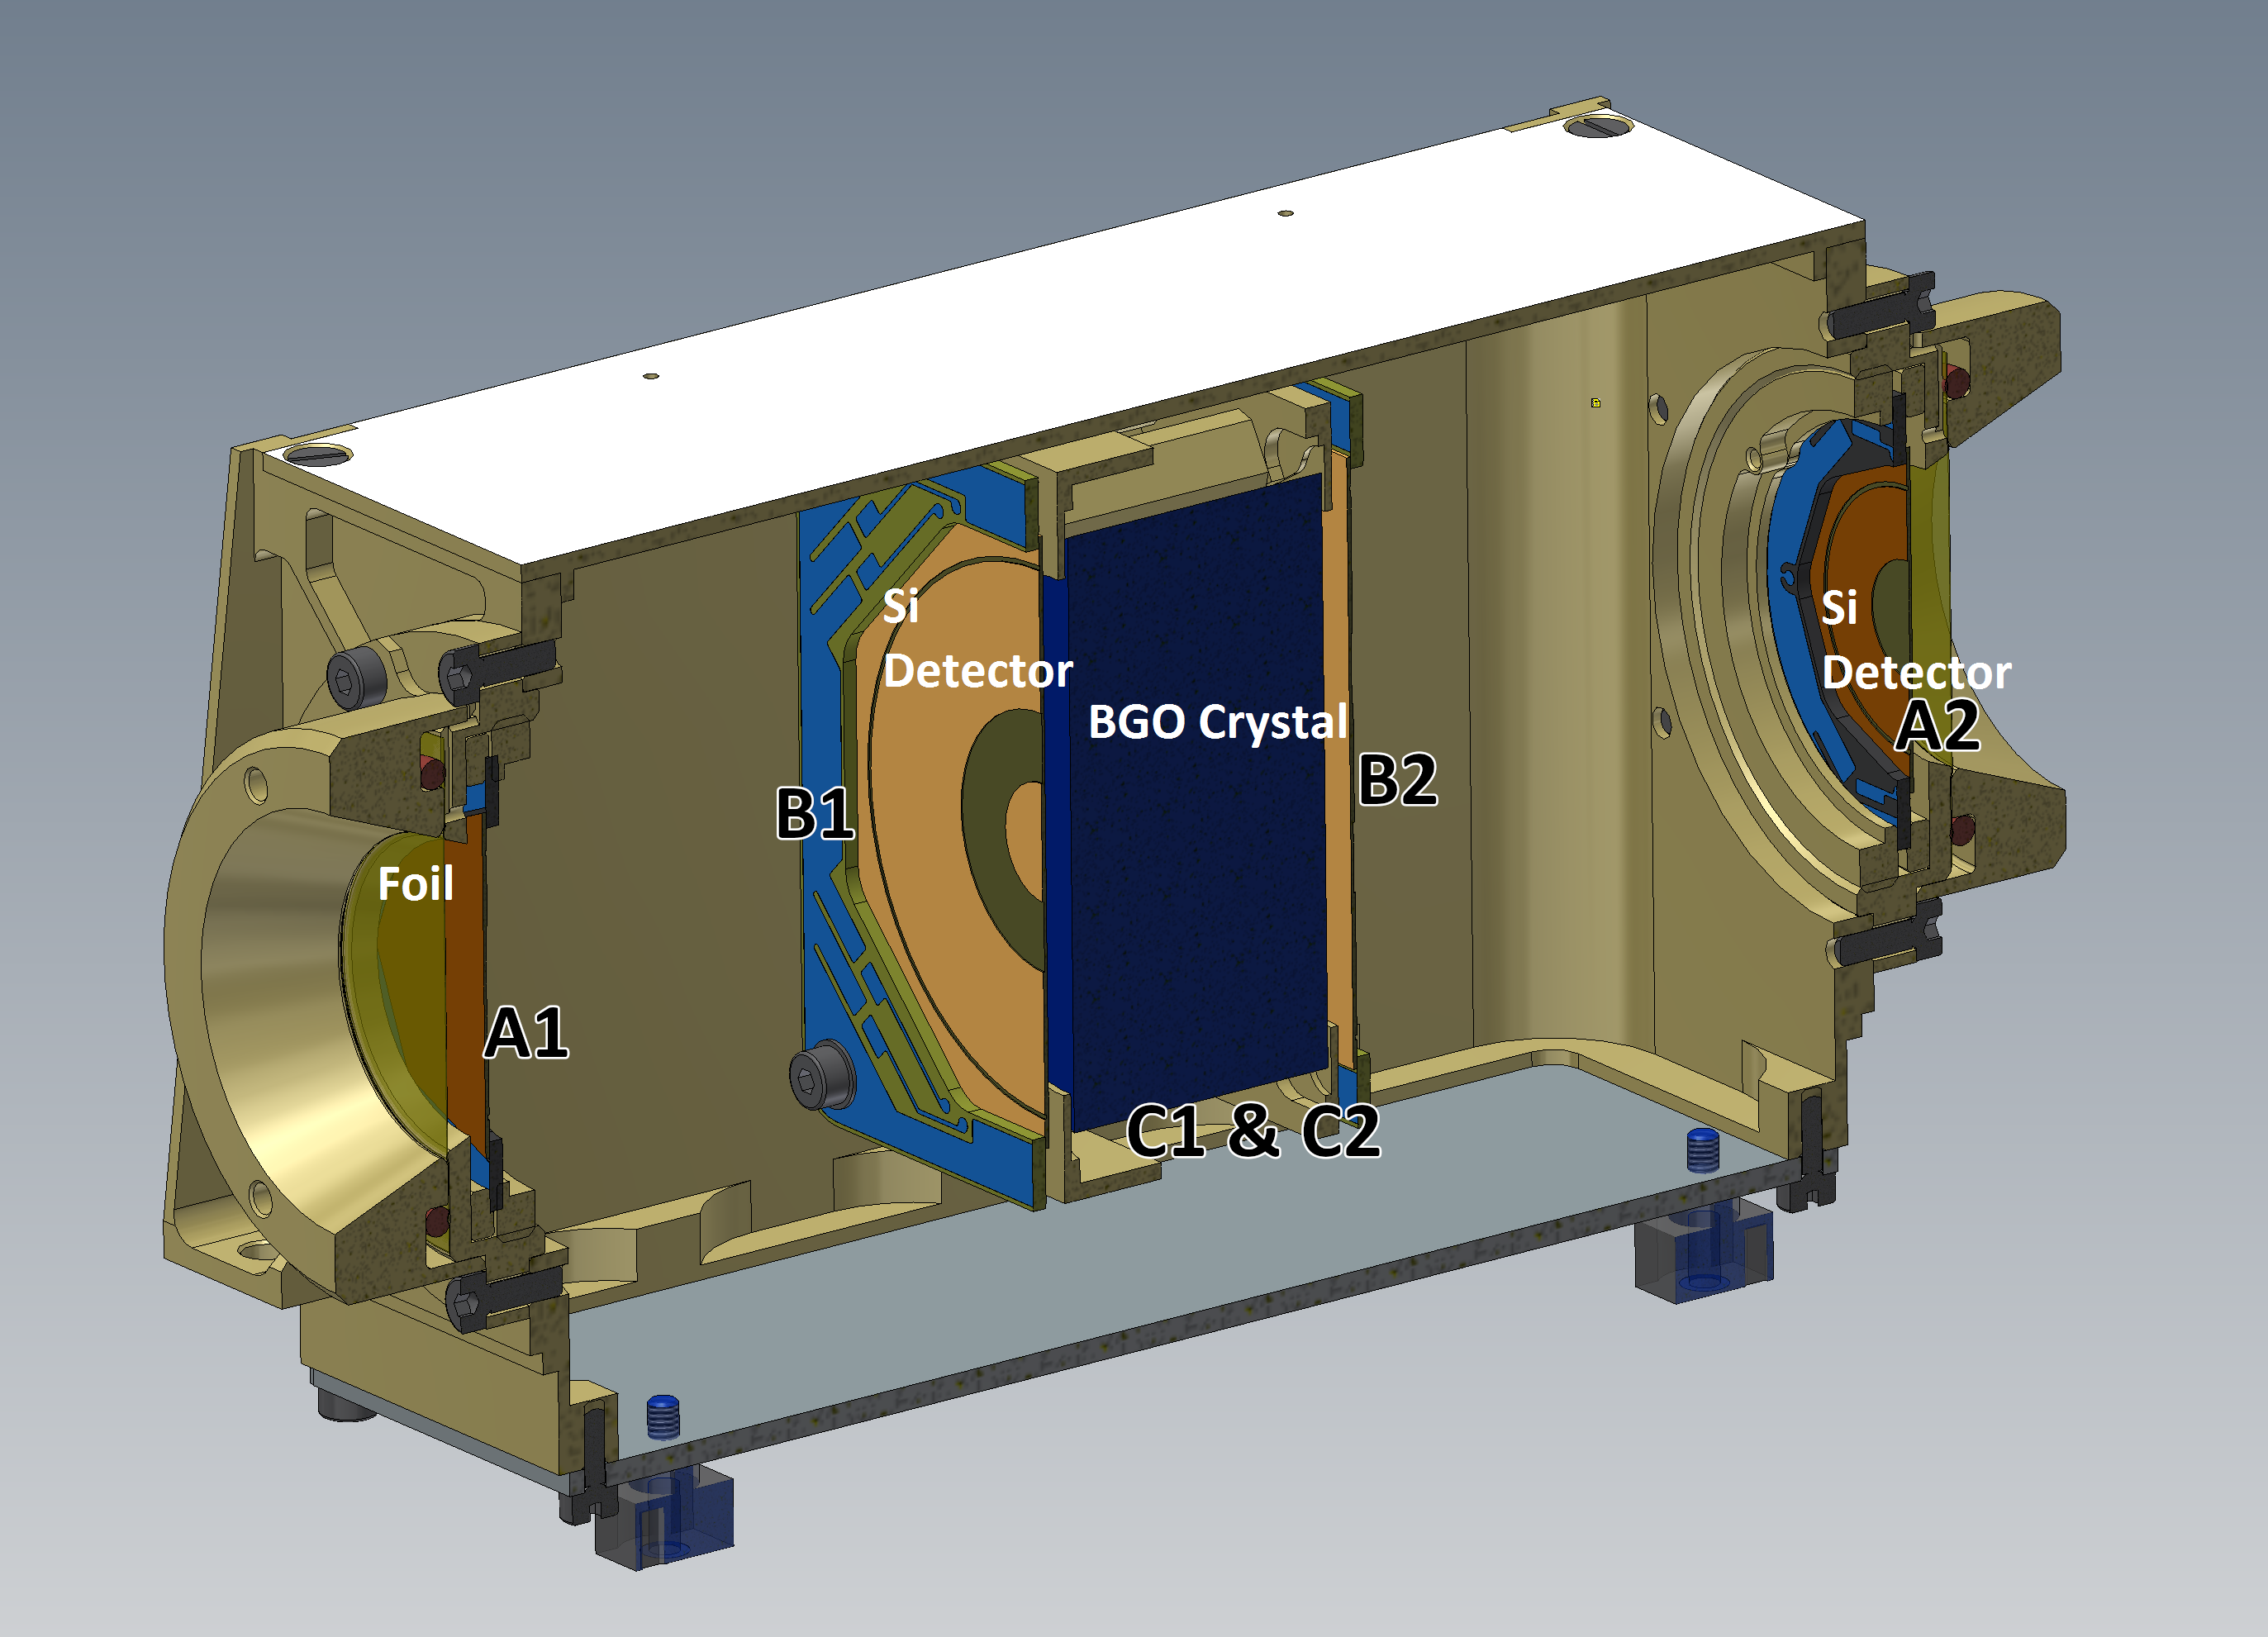
\includegraphics[width=0.7\textwidth]{images/het_enhanced.png}
% 		\label{subfig:het-sensorhead-cad}
% 	}\\
% 	\subfloat[Schematic diagram of the \ac{HET} sensor head. Exemplary particle trajectories ending up in different data products are shown by the arrows: \textcolor{red}{stopping in B}, \textcolor{green}{stopping in C}, \textcolor{blue}{penetrating}, \textcolor{Aquamarine}{GCR channel}, \textcolor{orange}{C single counter}.]{
% 		%\documentclass{standalone}
%\usepackage[dvipsnames]{xcolor}
%\usepackage{tikz}
%\usepackage{amsmath}
%\usepackage{siunitx}

%\usetikzlibrary{calc}
%\usetikzlibrary{decorations.pathmorphing}

%\definecolor{light-gray}{gray}{0.9}

%\begin{document}
\begin{tikzpicture}[scale=0.8]
    \tikzset{%
        add/.style args={#1 and #2}{
            to path={%
                ($(\tikztostart)!-#1!(\tikztotarget)$)--($(\tikztotarget)!-#2!(\tikztostart)$)%
                \tikztonodes},add/.default={.2 and .2}}
    }   
    
    \def\Sithickness{0.05}
    
    % A1
    \draw[fill=light-gray] (-\Sithickness, -0.87) rectangle (\Sithickness, 0.87) node[above,yshift=2mm]{A1};
    \draw (-\Sithickness, -0.4) -- (\Sithickness, -0.4);
    \draw (-\Sithickness, 0.4) -- (\Sithickness, 0.4);
    
    % B1
    \draw[fill=light-gray] (4.4-\Sithickness, -1.82) rectangle (4.4+\Sithickness, 1.82) node[above]{B1};
    \draw (4.4-\Sithickness, -0.4) -- (4.4+\Sithickness, -0.4);
    \draw (4.4-\Sithickness, 0.4) -- (4.4+\Sithickness, 0.4);
    \draw (4.4-\Sithickness, -0.87) -- (4.4+\Sithickness, -0.87);
    \draw (4.4-\Sithickness, 0.87) -- (4.4+\Sithickness, 0.87);
    
    % C
    \draw[fill=light-gray] (4.635, -1.75) rectangle ++(2, 3.5);
    \node[above, yshift=0.5mm] at (5.635, 1.75) {C};
    
    % B2
    \draw[fill=light-gray] (6.9-\Sithickness, -1.82) rectangle (6.9+\Sithickness, 1.82) node[above]{B2};
    \draw (6.9-\Sithickness, -0.4) -- (6.9+\Sithickness, -0.4);
    \draw (6.9-\Sithickness, 0.4) -- (6.9+\Sithickness, 0.4);
    \draw (6.9-\Sithickness, -0.87) -- (6.9+\Sithickness, -0.87);
    \draw (6.9-\Sithickness, 0.87) -- (6.9+\Sithickness, 0.87);
    
    % A2
    \draw[fill=light-gray] (11.3-\Sithickness, -0.87) rectangle (11.3+\Sithickness, 0.87) node[above,yshift=2mm]{A2};
    \draw (11.3-\Sithickness, -0.4) -- (11.3+\Sithickness, -0.4);
    \draw (11.3-\Sithickness, 0.4) -- (11.3+\Sithickness, 0.4);
    
    % FOV
    \draw[add=0.1 and 0, dashed, opacity=0.5] (0, -0.87) to (6.9, 1.82);
    \draw[add=0.1 and 0, dashed, opacity=0.5] (0, 0.87) to (6.9, -1.82);
    \draw[add=0.1 and 0, dashed, opacity=0.5] (11.3, -0.87) to (4.4, 1.82);
    \draw[add=0.1 and 0, dashed, opacity=0.5] (11.3, 0.87) to (4.4, -1.82);
    
    \draw[|<->|] (0, 0.87) ++ (180-21.45:0.5) arc (180-21.45:180+21.45:2.4+0.48) node[midway, left] {\small\SI{42.9}{\degree}};
    

    \draw[thick, red, -latex] (-0.2, 0.2) -- (4.4, 0.5);
    \draw[thick, green, -latex] (-0.2, 0) -- (5.7, 0.1);
    \draw[thick, blue, -latex] (-0.2, -0.2) -- (11.5, -0.5);
    \draw[thick, Aquamarine, -latex] (2.5, 2) -- (8.4, -2);
    \draw[thick, orange, -latex] (5.635, -2.3) -- (5.635, -1);
\end{tikzpicture}
%\end{document}
% 		\label{subfig:het-sensorhead-diagram}
% 	}
% 	\caption[\acs{HET} sensor head]{\acs{HET} sensor head}
% 	\label{fig:het-sensorhead}
% \end{figure}

% Charged particles that enter through one of the A detectors and then stop in B or C are measured in the \ac{HET} data products for stopping particles, which are defined using the ABnC and ABC coincidence conditions (as shown in red and green in \autoref{subfig:het-sensorhead-diagram}). These particles are fully analyzed using the $\dd E/\dd x$-$E$ method, i.e. their primary energy and charge can be directly determined.
% Ions with higher energies (e.g. $\gtrsim\SI{100}{\mega\electronvolt\per nuc}$ for protons and helium) penetrate the whole telescope (ABCBA coincidence, shown in blue in \autoref{subfig:het-sensorhead-diagram}). In this case, as with the penetrating particles in \ac{RAD}, the particles are not fully analyzed. Still, up to a few hundred \si{\mega\electronvolt\per nuc}, the particle direction and primary energy can be estimated based on the different \ac{LET} at each end of the telescope (e.g. in the A1 and A2 detectors).

% Similarly to \ac{RAD}, these energy-resolved stopping and penetrating particle data products are very useful for \ac{SEP} events as well as to calculate longterm \ac{GCR} spectra, but they do not have high enough count rates to study short-term variations of the \ac{GCR}. Alternatively, \ac{HET} also produces a data product using the BCB coincidence (irrespective of the A detectors, shown in turquoise in \autoref{subfig:het-sensorhead-diagram}), which significantly increases the opening angle at the cost of lower energy resolution and no separation of particle species. For this data product, only a 1D histogram of the energy deposit in C is stored. In addition, basic single detector count rates (level 1 trigger rates) without any coincidence conditions applied are available in \ac{HET}'s housekeeping data, which include particles entering \ac{HET} from any direction. In this case, the count rates for the C detector are best suited for measuring short-term variations due to the large volume of C. The response function of this single detector counter is derived in \autoref{chp:HETSimulation}.

% Further details about the design of the \ac{HET} instrument, the definition of its data products and their calibration can be found in \citet{Elftmann-2020-PhD}. 

% \section{Neutron monitor measurements}
% \label{sec:neutronmonitors}

% First developed in the 1950s \citep[see e.g.][]{Simpson-2000}, ground-based neutron monitors have historically been the most widely available instrument for the measurement of the cosmic ray flux at Earth. Neutron monitors measure secondary neutrons generated by the primary \ac{GCR} and \ac{SEP} particles in the Earth's atmosphere. They are typically large and heavy instruments, as one or more large tubes of lead are needed to achieve a sufficiently large detection efficiency for high-energy neutrons. Within a decade, such devices had been deployed at numerous locations around the globe, and many of them have been producing measurements almost continuously until the present day. Today, data from the global network of more than 50 neutron monitors \citep[e.g.][]{Moraal-2000} are archived at the \acl{NMDB}\acused{NMDB} \citep[\acs{NMDB},][]{Steigies-2009}\footnote{\url{https://www.nmdb.eu}}, and many of these stations are also providing realtime data through \ac{NMDB}.

% Similar to \ac{RAD} on Mars (\autoref{sec:mslrad}), neutron monitor measurements are influenced by the Earth's atmosphere, but also by the magnetic field, which is negligible at Mars. Thus, any cosmic ray particle needs a certain minimum energy, the so-called cutoff energy, to be able to pass through the magnetosphere and produce a secondary neutron in the atmosphere, which then reaches the ground and can be detected by a neutron monitor. The atmospheric effect is mainly dependent on the altitude as well as the atmospheric pressure, while the magnetospheric effect depends on the geographic location, particularly the latitude. At the poles, where the magnetic field lines are nearly vertical, the magnetic cutoff decreases to zero, and thus the atmospheric effect is dominant in this case.

% The cutoff energy is often also expressed in terms of a rigidity
% \begin{equation}
% 	R = \frac{pc}{q},
% \end{equation}
% a quantity which is given in units of volts (\si{V}). $p$ is the particle's momentum, $q$ its charge and $c$ the speed of light. The benefit of using rigidities instead of (kinetic) energies is that particles with the same rigidity also have the same gyroradius in the magnetic field independent of the particle species. Using relativistic relations, $R$ can be rewritten in terms of the particle's charge $q = Ze$, rest mass $m_0$ and kinetic energy $E_\text{kin}$ as:
% \begin{equation}
%     R = \frac{1}{Ze} \sqrt{E_\text{kin}(E_\text{kin} + 2 m_0 c^2)}
% \end{equation}
% \citep[see e.g.][for the detailed derivation]{Moraal-2013}, which approaches $R \approx E_\text{kin}/(Ze)$ for highly relativistic particles ($E_\text{kin}\gg m_0 c^2$). So, for example, a \SI{100}{\giga\electronvolt} proton ($Z=1$) has a rigidity of approximately \SI{100}{\giga\volt}.

% Magnetic cutoff rigidities and the resulting response functions for neutron monitors, which take both the magnetospheric and the atmospheric effect into account, have been calculated by e.g. \citet{Clem-Dorman-2000,Smart-Shea-2001,Smart-Shea-2008}. The South Pole Neutron Monitor, located at the geographic south pole (\SI{90}{\degree} S) and \SI{2820}{\meter} altitude --- next to the Amundsen-Scott research station --- is the most sensitive neutron monitor station, as its magnetic cutoff is negligible and the atmospheric cutoff is also lower than at sea level. This makes it especially well suited for the detection of \acp{FD}, as they typically have larger amplitudes at lower energies (see \autoref{sec:forbush}). The South Pole Neutron Monitor will be used multiple times in this thesis to provide \ac{FD} observations at Earth that can be compared to the Mars or \ac{SolO} data.

% In addition to using single neutron monitors, an inversion method has also been developed to reconstruct the variation of the \ac{GCR} flux at a certain rigidity above the atmosphere and magnetosphere from the global network of neutron monitors. This so-called \ac{GSM} produces results that are independent of the characteristics of a single neutron monitor station. It is described in detail by \citet{Belov2018}, and is used e.g. as a basis for the extensive catalog of Forbush decreases at Earth compiled by the Russian Space Weather Prediction Center (IZMIRAN)\footnote{\url{http://spaceweather.izmiran.ru/eng/dbs.html}}, which is also employed in this thesis for statistical studies in the publication by \citet{Forstner-2020}.

% \section{The STEREO Heliospheric Imagers}
% \label{sec:stereohi}

% Launched in 2006, the \acl{STEREO}\acused{STEREO} \citep[\acs{STEREO},][]{Russell-2008-STEREO} is a NASA mission that enabled a stereoscopic view of the Sun for the first time. It consists of two largely identical spacecraft that were placed in an orbit around the Sun at distances close to \SI{1}{\AU}, carrying both in situ and remote sensing instruments. The \ac{STEREO}-A (Ahead) spacecraft is placed a bit closer to the Sun than Earth, while \ac{STEREO}-B (Behind) is a bit farther away. This caused the two spacecraft to slowly drift away from Earth, as A orbits the Sun slightly faster than Earth, and B slightly slower. 5 years later, the spacecraft were separated by \SI{180}{\degree} in longitude, and this made it possible to observe all sides of the Sun (except the poles) simultaneously for the first time. In 2015, the two spacecraft reached a solar conjunction, passing behind the Sun as seen from Earth, and are coming closer to Earth again ever since. Their next close approach to Earth is expected in 2023, 17 years after launch.

% With a planned mission duration of only 2 years, the \ac{STEREO} spacecraft were never designed to survive a solar conjunction, during which communication with Earth is not possible for several months, so significant configuration changes were necessary in the flight software. Unfortunately, while testing the new configuration designed for the solar conjunction phase, communications with the \ac{STEREO}-B spacecraft were lost on October 1, 2014, so since this date, science data are only available from \ac{STEREO}-A. It is believed that this was due to a temporary failure of the star tracker coinciding with incorrect data transmitted from one of the gyroscopes, causing the spacecraft to start spinning while it fired its thrusters in an attempt to compensate for the perceived rotation \citep{Cox-2018}. In this state, the spacecraft battery drained quickly as the solar panels were pointed toward the Sun only for a fraction of the time. The communications link to the spacecraft was restored for a few weeks in 2016, but the following attempt to re-stabilize the spacecraft was unsuccessful and connection was lost again. Recovery will be re-attempted when \ac{STEREO}-B comes closer to Earth in the next few years.

% Apart from three in situ experiments investigating the local solar wind plasma, energetic particles, magnetic fields and radio waves, the scientific payload onboard the \ac{STEREO} spacecraft also includes the \acl{SECCHI}\acused{SECCHI} \citep[\acs{SECCHI},][]{Howard-2008-SECCHI}, a suite of remote sensing instruments consisting of five telescopes (\autoref{tab:secchi_telescopes}) with different fields of view (from the solar disk to almost \SI{90}{\degree}) and wavelengths (\ac{EUV} and visible light, ``white light''). The \ac{EUV} imager (EUVI) observes the solar disk directly in four different wavelength bands, while the white-light coronagraphs COR1 and COR2 use an occulting disk in their center to cover the solar disk and observe the surrounding corona. Similar types of instruments have already been available from the Earth point of view, e.g. on the \ac{SOHO} spacecraft launched in the 1990s and its predecessors.
% On the other hand, the \aclp{HI}\acused{HI} \citep[\acs{HI},][]{Eyles2009-STEREOHI} are a relatively new type of instrument that had first been demonstrated in 2003 with the Solar Mass Ejection Imager \citep[SMEI,][]{Eyles-2003-SMEI} onboard the \textit{Coriolis} spacecraft. These white-light telescopes provide a very wide field of view between \SI{4}{\degree} and \SI{88.7}{\degree} from the Sun in the ecliptic plane and up to $\pm\SI{35}{\degree}$ in the perpendicular direction. With these data, \acp{CME} can be directly tracked from near the Sun out into interplanetary space. In contrast to the other telescopes, the \acp{HI} have rectangular fields of view directed away from the Sun towards one side --- therefore, the \ac{STEREO} spacecraft are always rotated so that the \acp{HI} can best observe the Sun-Earth line.

% \begin{table}
%     \begin{tabular}{llll}
%         \toprule
%     	Telescope & Description                & Wavelength                                                                         & Field of view                   \\
%         \midrule
%     	EUVI      & \ac{EUV} imager & \SI{171}{\angstrom}, \SI{195}{\angstrom}, \SI{284}{\angstrom}, \SI{304}{\angstrom} & \SIrange{0}{1.7}{\solarradius}  \\
%     	COR1      & inner coronagraph          & white light                                                                        & \SIrange{1.4}{4}{\solarradius}  \\
%     	COR2      & outer coronagraph          & white light                                                                        & \SIrange{2.5}{15}{\solarradius} \\
%     	HI1       & heliospheric imager 1  & white light                                                                        & \SIrange{4}{24}{\degree}        \\
%     	HI2       & heliospheric imager 2  & white light                                                                        & \SIrange{18.7}{88.7}{\degree}       \\
%         \bottomrule
%     \end{tabular}
%     \caption[Properties of the \acs{STEREO} \acs{SECCHI} telescopes]{Properties of the \acs{STEREO} \acs{SECCHI} telescopes.}
%     \label{tab:secchi_telescopes}
% \end{table}

% \autoref{fig:secchifov} demonstrates the different fields of view of the \ac{SECCHI} instruments. This composite image, which was constructed using the SunPy software toolkit \citep{sunpy_community2020}, shows the April 15, 2020 \ac{CME} \citep[see also \autoref{chp:solo} /][]{Forstner-2021-SolO}, which has just entered the HI1 field of view at this time. In addition, signatures of four solar system planets (Venus, Earth, Jupiter and Saturn) can be seen in the \acp{HI} telescopes, as well as the diagonal band of the Milky Way in HI2. The near-vertical trails in the \ac{HI} images are an instrumental artifact caused by the high relative brightness of the planets and some stars in combination with the column-wise sensor readout and the lack of a mechanical shutter.

% \begin{figure}
%     \centering
%     %% Creator: Matplotlib, PGF backend
%%
%% To include the figure in your LaTeX document, write
%%   \input{<filename>.pgf}
%%
%% Make sure the required packages are loaded in your preamble
%%   \usepackage{pgf}
%%
%% and, on pdftex
%%   \usepackage[utf8]{inputenc}\DeclareUnicodeCharacter{2212}{-}
%%
%% or, on luatex and xetex
%%   \usepackage{unicode-math}
%%
%% Figures using additional raster images can only be included by \input if
%% they are in the same directory as the main LaTeX file. For loading figures
%% from other directories you can use the `import` package
%%   \usepackage{import}
%%
%% and then include the figures with
%%   \import{<path to file>}{<filename>.pgf}
%%
%% Matplotlib used the following preamble
%%   \usepackage{fontspec}
%%
\begingroup%
\makeatletter%
\begin{pgfpicture}%
\pgfpathrectangle{\pgfpointorigin}{\pgfqpoint{5.200000in}{3.500000in}}%
\pgfusepath{use as bounding box, clip}%
\begin{pgfscope}%
\pgfsetbuttcap%
\pgfsetmiterjoin%
\definecolor{currentfill}{rgb}{1.000000,1.000000,1.000000}%
\pgfsetfillcolor{currentfill}%
\pgfsetlinewidth{0.000000pt}%
\definecolor{currentstroke}{rgb}{1.000000,1.000000,1.000000}%
\pgfsetstrokecolor{currentstroke}%
\pgfsetdash{}{0pt}%
\pgfpathmoveto{\pgfqpoint{0.000000in}{0.000000in}}%
\pgfpathlineto{\pgfqpoint{5.200000in}{0.000000in}}%
\pgfpathlineto{\pgfqpoint{5.200000in}{3.500000in}}%
\pgfpathlineto{\pgfqpoint{0.000000in}{3.500000in}}%
\pgfpathclose%
\pgfusepath{fill}%
\end{pgfscope}%
\begin{pgfscope}%
\pgfsetbuttcap%
\pgfsetmiterjoin%
\definecolor{currentfill}{rgb}{1.000000,1.000000,1.000000}%
\pgfsetfillcolor{currentfill}%
\pgfsetlinewidth{0.000000pt}%
\definecolor{currentstroke}{rgb}{0.000000,0.000000,0.000000}%
\pgfsetstrokecolor{currentstroke}%
\pgfsetstrokeopacity{0.000000}%
\pgfsetdash{}{0pt}%
\pgfpathmoveto{\pgfqpoint{0.582966in}{0.478438in}}%
\pgfpathlineto{\pgfqpoint{5.065000in}{0.478438in}}%
\pgfpathlineto{\pgfqpoint{5.065000in}{3.355531in}}%
\pgfpathlineto{\pgfqpoint{0.582966in}{3.355531in}}%
\pgfpathclose%
\pgfusepath{fill}%
\end{pgfscope}%
\begin{pgfscope}%
\pgfpathrectangle{\pgfqpoint{0.582966in}{0.478438in}}{\pgfqpoint{4.482034in}{2.877093in}}%
\pgfusepath{clip}%
\pgfsys@transformshift{1.710883in}{0.478438in}%
\pgftext[left,bottom]{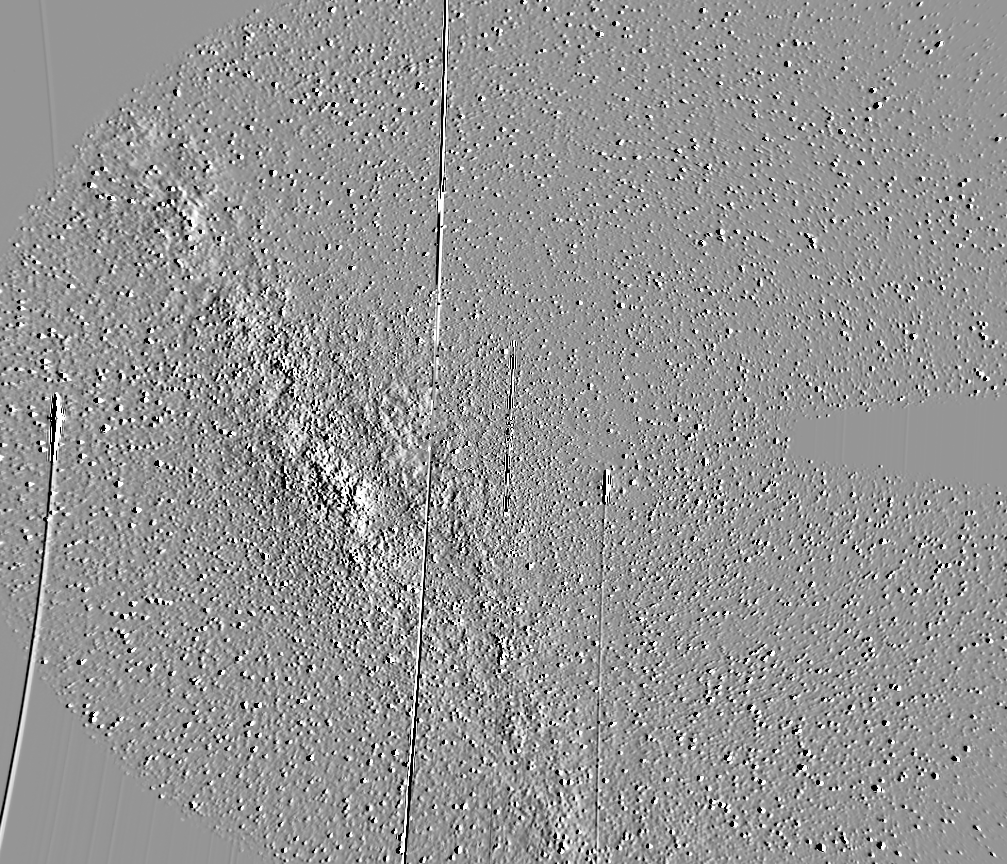
\includegraphics[interpolate=true,width=3.356667in,height=2.880000in]{plots/secchi_fov-img0.png}}%
\end{pgfscope}%
\begin{pgfscope}%
\pgfpathrectangle{\pgfqpoint{0.582966in}{0.478438in}}{\pgfqpoint{4.482034in}{2.877093in}}%
\pgfusepath{clip}%
\pgfsetbuttcap%
\pgfsetmiterjoin%
\pgfsetlinewidth{1.003750pt}%
\definecolor{currentstroke}{rgb}{0.000000,0.000000,0.000000}%
\pgfsetstrokecolor{currentstroke}%
\pgfsetdash{}{0pt}%
\pgfpathmoveto{\pgfqpoint{1.710883in}{0.478438in}}%
\pgfpathlineto{\pgfqpoint{5.065000in}{0.478438in}}%
\pgfpathlineto{\pgfqpoint{5.065000in}{3.355531in}}%
\pgfpathlineto{\pgfqpoint{1.710883in}{3.355531in}}%
\pgfpathclose%
\pgfusepath{stroke}%
\end{pgfscope}%
\begin{pgfscope}%
\definecolor{textcolor}{rgb}{0.000000,0.000000,0.000000}%
\pgfsetstrokecolor{textcolor}%
\pgfsetfillcolor{textcolor}%
\pgftext[x=1.809694in,y=0.577249in,left,base]{\color{textcolor}\rmfamily\fontsize{12.000000}{14.400000}\bfseries\selectfont HI2}%
\end{pgfscope}%
\begin{pgfscope}%
\pgfsetbuttcap%
\pgfsetroundjoin%
\definecolor{currentfill}{rgb}{0.000000,0.000000,0.000000}%
\pgfsetfillcolor{currentfill}%
\pgfsetlinewidth{0.803000pt}%
\definecolor{currentstroke}{rgb}{0.000000,0.000000,0.000000}%
\pgfsetstrokecolor{currentstroke}%
\pgfsetdash{}{0pt}%
\pgfsys@defobject{currentmarker}{\pgfqpoint{0.000000in}{-0.048611in}}{\pgfqpoint{0.000000in}{0.000000in}}{%
\pgfpathmoveto{\pgfqpoint{0.000000in}{0.000000in}}%
\pgfpathlineto{\pgfqpoint{0.000000in}{-0.048611in}}%
\pgfusepath{stroke,fill}%
}%
\begin{pgfscope}%
\pgfsys@transformshift{0.790447in}{0.478438in}%
\pgfsys@useobject{currentmarker}{}%
\end{pgfscope}%
\end{pgfscope}%
\begin{pgfscope}%
\definecolor{textcolor}{rgb}{0.000000,0.000000,0.000000}%
\pgfsetstrokecolor{textcolor}%
\pgfsetfillcolor{textcolor}%
\pgftext[x=0.790447in,y=0.381216in,,top]{\color{textcolor}\rmfamily\fontsize{9.000000}{10.800000}\selectfont 0}%
\end{pgfscope}%
\begin{pgfscope}%
\pgfsetbuttcap%
\pgfsetroundjoin%
\definecolor{currentfill}{rgb}{0.000000,0.000000,0.000000}%
\pgfsetfillcolor{currentfill}%
\pgfsetlinewidth{0.803000pt}%
\definecolor{currentstroke}{rgb}{0.000000,0.000000,0.000000}%
\pgfsetstrokecolor{currentstroke}%
\pgfsetdash{}{0pt}%
\pgfsys@defobject{currentmarker}{\pgfqpoint{0.000000in}{-0.048611in}}{\pgfqpoint{0.000000in}{0.000000in}}{%
\pgfpathmoveto{\pgfqpoint{0.000000in}{0.000000in}}%
\pgfpathlineto{\pgfqpoint{0.000000in}{-0.048611in}}%
\pgfusepath{stroke,fill}%
}%
\begin{pgfscope}%
\pgfsys@transformshift{1.284501in}{0.478438in}%
\pgfsys@useobject{currentmarker}{}%
\end{pgfscope}%
\end{pgfscope}%
\begin{pgfscope}%
\definecolor{textcolor}{rgb}{0.000000,0.000000,0.000000}%
\pgfsetstrokecolor{textcolor}%
\pgfsetfillcolor{textcolor}%
\pgftext[x=1.284501in,y=0.381216in,,top]{\color{textcolor}\rmfamily\fontsize{9.000000}{10.800000}\selectfont 10}%
\end{pgfscope}%
\begin{pgfscope}%
\pgfsetbuttcap%
\pgfsetroundjoin%
\definecolor{currentfill}{rgb}{0.000000,0.000000,0.000000}%
\pgfsetfillcolor{currentfill}%
\pgfsetlinewidth{0.803000pt}%
\definecolor{currentstroke}{rgb}{0.000000,0.000000,0.000000}%
\pgfsetstrokecolor{currentstroke}%
\pgfsetdash{}{0pt}%
\pgfsys@defobject{currentmarker}{\pgfqpoint{0.000000in}{-0.048611in}}{\pgfqpoint{0.000000in}{0.000000in}}{%
\pgfpathmoveto{\pgfqpoint{0.000000in}{0.000000in}}%
\pgfpathlineto{\pgfqpoint{0.000000in}{-0.048611in}}%
\pgfusepath{stroke,fill}%
}%
\begin{pgfscope}%
\pgfsys@transformshift{1.778554in}{0.478438in}%
\pgfsys@useobject{currentmarker}{}%
\end{pgfscope}%
\end{pgfscope}%
\begin{pgfscope}%
\definecolor{textcolor}{rgb}{0.000000,0.000000,0.000000}%
\pgfsetstrokecolor{textcolor}%
\pgfsetfillcolor{textcolor}%
\pgftext[x=1.778554in,y=0.381216in,,top]{\color{textcolor}\rmfamily\fontsize{9.000000}{10.800000}\selectfont 20}%
\end{pgfscope}%
\begin{pgfscope}%
\pgfsetbuttcap%
\pgfsetroundjoin%
\definecolor{currentfill}{rgb}{0.000000,0.000000,0.000000}%
\pgfsetfillcolor{currentfill}%
\pgfsetlinewidth{0.803000pt}%
\definecolor{currentstroke}{rgb}{0.000000,0.000000,0.000000}%
\pgfsetstrokecolor{currentstroke}%
\pgfsetdash{}{0pt}%
\pgfsys@defobject{currentmarker}{\pgfqpoint{0.000000in}{-0.048611in}}{\pgfqpoint{0.000000in}{0.000000in}}{%
\pgfpathmoveto{\pgfqpoint{0.000000in}{0.000000in}}%
\pgfpathlineto{\pgfqpoint{0.000000in}{-0.048611in}}%
\pgfusepath{stroke,fill}%
}%
\begin{pgfscope}%
\pgfsys@transformshift{2.272608in}{0.478438in}%
\pgfsys@useobject{currentmarker}{}%
\end{pgfscope}%
\end{pgfscope}%
\begin{pgfscope}%
\definecolor{textcolor}{rgb}{0.000000,0.000000,0.000000}%
\pgfsetstrokecolor{textcolor}%
\pgfsetfillcolor{textcolor}%
\pgftext[x=2.272608in,y=0.381216in,,top]{\color{textcolor}\rmfamily\fontsize{9.000000}{10.800000}\selectfont 30}%
\end{pgfscope}%
\begin{pgfscope}%
\pgfsetbuttcap%
\pgfsetroundjoin%
\definecolor{currentfill}{rgb}{0.000000,0.000000,0.000000}%
\pgfsetfillcolor{currentfill}%
\pgfsetlinewidth{0.803000pt}%
\definecolor{currentstroke}{rgb}{0.000000,0.000000,0.000000}%
\pgfsetstrokecolor{currentstroke}%
\pgfsetdash{}{0pt}%
\pgfsys@defobject{currentmarker}{\pgfqpoint{0.000000in}{-0.048611in}}{\pgfqpoint{0.000000in}{0.000000in}}{%
\pgfpathmoveto{\pgfqpoint{0.000000in}{0.000000in}}%
\pgfpathlineto{\pgfqpoint{0.000000in}{-0.048611in}}%
\pgfusepath{stroke,fill}%
}%
\begin{pgfscope}%
\pgfsys@transformshift{2.766662in}{0.478438in}%
\pgfsys@useobject{currentmarker}{}%
\end{pgfscope}%
\end{pgfscope}%
\begin{pgfscope}%
\definecolor{textcolor}{rgb}{0.000000,0.000000,0.000000}%
\pgfsetstrokecolor{textcolor}%
\pgfsetfillcolor{textcolor}%
\pgftext[x=2.766662in,y=0.381216in,,top]{\color{textcolor}\rmfamily\fontsize{9.000000}{10.800000}\selectfont 40}%
\end{pgfscope}%
\begin{pgfscope}%
\pgfsetbuttcap%
\pgfsetroundjoin%
\definecolor{currentfill}{rgb}{0.000000,0.000000,0.000000}%
\pgfsetfillcolor{currentfill}%
\pgfsetlinewidth{0.803000pt}%
\definecolor{currentstroke}{rgb}{0.000000,0.000000,0.000000}%
\pgfsetstrokecolor{currentstroke}%
\pgfsetdash{}{0pt}%
\pgfsys@defobject{currentmarker}{\pgfqpoint{0.000000in}{-0.048611in}}{\pgfqpoint{0.000000in}{0.000000in}}{%
\pgfpathmoveto{\pgfqpoint{0.000000in}{0.000000in}}%
\pgfpathlineto{\pgfqpoint{0.000000in}{-0.048611in}}%
\pgfusepath{stroke,fill}%
}%
\begin{pgfscope}%
\pgfsys@transformshift{3.260715in}{0.478438in}%
\pgfsys@useobject{currentmarker}{}%
\end{pgfscope}%
\end{pgfscope}%
\begin{pgfscope}%
\definecolor{textcolor}{rgb}{0.000000,0.000000,0.000000}%
\pgfsetstrokecolor{textcolor}%
\pgfsetfillcolor{textcolor}%
\pgftext[x=3.260715in,y=0.381216in,,top]{\color{textcolor}\rmfamily\fontsize{9.000000}{10.800000}\selectfont 50}%
\end{pgfscope}%
\begin{pgfscope}%
\pgfsetbuttcap%
\pgfsetroundjoin%
\definecolor{currentfill}{rgb}{0.000000,0.000000,0.000000}%
\pgfsetfillcolor{currentfill}%
\pgfsetlinewidth{0.803000pt}%
\definecolor{currentstroke}{rgb}{0.000000,0.000000,0.000000}%
\pgfsetstrokecolor{currentstroke}%
\pgfsetdash{}{0pt}%
\pgfsys@defobject{currentmarker}{\pgfqpoint{0.000000in}{-0.048611in}}{\pgfqpoint{0.000000in}{0.000000in}}{%
\pgfpathmoveto{\pgfqpoint{0.000000in}{0.000000in}}%
\pgfpathlineto{\pgfqpoint{0.000000in}{-0.048611in}}%
\pgfusepath{stroke,fill}%
}%
\begin{pgfscope}%
\pgfsys@transformshift{3.754769in}{0.478438in}%
\pgfsys@useobject{currentmarker}{}%
\end{pgfscope}%
\end{pgfscope}%
\begin{pgfscope}%
\definecolor{textcolor}{rgb}{0.000000,0.000000,0.000000}%
\pgfsetstrokecolor{textcolor}%
\pgfsetfillcolor{textcolor}%
\pgftext[x=3.754769in,y=0.381216in,,top]{\color{textcolor}\rmfamily\fontsize{9.000000}{10.800000}\selectfont 60}%
\end{pgfscope}%
\begin{pgfscope}%
\pgfsetbuttcap%
\pgfsetroundjoin%
\definecolor{currentfill}{rgb}{0.000000,0.000000,0.000000}%
\pgfsetfillcolor{currentfill}%
\pgfsetlinewidth{0.803000pt}%
\definecolor{currentstroke}{rgb}{0.000000,0.000000,0.000000}%
\pgfsetstrokecolor{currentstroke}%
\pgfsetdash{}{0pt}%
\pgfsys@defobject{currentmarker}{\pgfqpoint{0.000000in}{-0.048611in}}{\pgfqpoint{0.000000in}{0.000000in}}{%
\pgfpathmoveto{\pgfqpoint{0.000000in}{0.000000in}}%
\pgfpathlineto{\pgfqpoint{0.000000in}{-0.048611in}}%
\pgfusepath{stroke,fill}%
}%
\begin{pgfscope}%
\pgfsys@transformshift{4.248823in}{0.478438in}%
\pgfsys@useobject{currentmarker}{}%
\end{pgfscope}%
\end{pgfscope}%
\begin{pgfscope}%
\definecolor{textcolor}{rgb}{0.000000,0.000000,0.000000}%
\pgfsetstrokecolor{textcolor}%
\pgfsetfillcolor{textcolor}%
\pgftext[x=4.248823in,y=0.381216in,,top]{\color{textcolor}\rmfamily\fontsize{9.000000}{10.800000}\selectfont 70}%
\end{pgfscope}%
\begin{pgfscope}%
\pgfsetbuttcap%
\pgfsetroundjoin%
\definecolor{currentfill}{rgb}{0.000000,0.000000,0.000000}%
\pgfsetfillcolor{currentfill}%
\pgfsetlinewidth{0.803000pt}%
\definecolor{currentstroke}{rgb}{0.000000,0.000000,0.000000}%
\pgfsetstrokecolor{currentstroke}%
\pgfsetdash{}{0pt}%
\pgfsys@defobject{currentmarker}{\pgfqpoint{0.000000in}{-0.048611in}}{\pgfqpoint{0.000000in}{0.000000in}}{%
\pgfpathmoveto{\pgfqpoint{0.000000in}{0.000000in}}%
\pgfpathlineto{\pgfqpoint{0.000000in}{-0.048611in}}%
\pgfusepath{stroke,fill}%
}%
\begin{pgfscope}%
\pgfsys@transformshift{4.742876in}{0.478438in}%
\pgfsys@useobject{currentmarker}{}%
\end{pgfscope}%
\end{pgfscope}%
\begin{pgfscope}%
\definecolor{textcolor}{rgb}{0.000000,0.000000,0.000000}%
\pgfsetstrokecolor{textcolor}%
\pgfsetfillcolor{textcolor}%
\pgftext[x=4.742876in,y=0.381216in,,top]{\color{textcolor}\rmfamily\fontsize{9.000000}{10.800000}\selectfont 80}%
\end{pgfscope}%
\begin{pgfscope}%
\definecolor{textcolor}{rgb}{0.000000,0.000000,0.000000}%
\pgfsetstrokecolor{textcolor}%
\pgfsetfillcolor{textcolor}%
\pgftext[x=2.823983in,y=0.214660in,,top]{\color{textcolor}\rmfamily\fontsize{9.000000}{10.800000}\selectfont Helioprojective Longitude [°]}%
\end{pgfscope}%
\begin{pgfscope}%
\pgfsetbuttcap%
\pgfsetroundjoin%
\definecolor{currentfill}{rgb}{0.000000,0.000000,0.000000}%
\pgfsetfillcolor{currentfill}%
\pgfsetlinewidth{0.803000pt}%
\definecolor{currentstroke}{rgb}{0.000000,0.000000,0.000000}%
\pgfsetstrokecolor{currentstroke}%
\pgfsetdash{}{0pt}%
\pgfsys@defobject{currentmarker}{\pgfqpoint{-0.048611in}{0.000000in}}{\pgfqpoint{-0.000000in}{0.000000in}}{%
\pgfpathmoveto{\pgfqpoint{-0.000000in}{0.000000in}}%
\pgfpathlineto{\pgfqpoint{-0.048611in}{0.000000in}}%
\pgfusepath{stroke,fill}%
}%
\begin{pgfscope}%
\pgfsys@transformshift{0.582966in}{0.570008in}%
\pgfsys@useobject{currentmarker}{}%
\end{pgfscope}%
\end{pgfscope}%
\begin{pgfscope}%
\definecolor{textcolor}{rgb}{0.000000,0.000000,0.000000}%
\pgfsetstrokecolor{textcolor}%
\pgfsetfillcolor{textcolor}%
\pgftext[x=0.314369in, y=0.526633in, left, base]{\color{textcolor}\rmfamily\fontsize{9.000000}{10.800000}\selectfont -30}%
\end{pgfscope}%
\begin{pgfscope}%
\pgfsetbuttcap%
\pgfsetroundjoin%
\definecolor{currentfill}{rgb}{0.000000,0.000000,0.000000}%
\pgfsetfillcolor{currentfill}%
\pgfsetlinewidth{0.803000pt}%
\definecolor{currentstroke}{rgb}{0.000000,0.000000,0.000000}%
\pgfsetstrokecolor{currentstroke}%
\pgfsetdash{}{0pt}%
\pgfsys@defobject{currentmarker}{\pgfqpoint{-0.048611in}{0.000000in}}{\pgfqpoint{-0.000000in}{0.000000in}}{%
\pgfpathmoveto{\pgfqpoint{-0.000000in}{0.000000in}}%
\pgfpathlineto{\pgfqpoint{-0.048611in}{0.000000in}}%
\pgfusepath{stroke,fill}%
}%
\begin{pgfscope}%
\pgfsys@transformshift{0.582966in}{0.817035in}%
\pgfsys@useobject{currentmarker}{}%
\end{pgfscope}%
\end{pgfscope}%
\begin{pgfscope}%
\definecolor{textcolor}{rgb}{0.000000,0.000000,0.000000}%
\pgfsetstrokecolor{textcolor}%
\pgfsetfillcolor{textcolor}%
\pgftext[x=0.314369in, y=0.773660in, left, base]{\color{textcolor}\rmfamily\fontsize{9.000000}{10.800000}\selectfont -25}%
\end{pgfscope}%
\begin{pgfscope}%
\pgfsetbuttcap%
\pgfsetroundjoin%
\definecolor{currentfill}{rgb}{0.000000,0.000000,0.000000}%
\pgfsetfillcolor{currentfill}%
\pgfsetlinewidth{0.803000pt}%
\definecolor{currentstroke}{rgb}{0.000000,0.000000,0.000000}%
\pgfsetstrokecolor{currentstroke}%
\pgfsetdash{}{0pt}%
\pgfsys@defobject{currentmarker}{\pgfqpoint{-0.048611in}{0.000000in}}{\pgfqpoint{-0.000000in}{0.000000in}}{%
\pgfpathmoveto{\pgfqpoint{-0.000000in}{0.000000in}}%
\pgfpathlineto{\pgfqpoint{-0.048611in}{0.000000in}}%
\pgfusepath{stroke,fill}%
}%
\begin{pgfscope}%
\pgfsys@transformshift{0.582966in}{1.064061in}%
\pgfsys@useobject{currentmarker}{}%
\end{pgfscope}%
\end{pgfscope}%
\begin{pgfscope}%
\definecolor{textcolor}{rgb}{0.000000,0.000000,0.000000}%
\pgfsetstrokecolor{textcolor}%
\pgfsetfillcolor{textcolor}%
\pgftext[x=0.314369in, y=1.020686in, left, base]{\color{textcolor}\rmfamily\fontsize{9.000000}{10.800000}\selectfont -20}%
\end{pgfscope}%
\begin{pgfscope}%
\pgfsetbuttcap%
\pgfsetroundjoin%
\definecolor{currentfill}{rgb}{0.000000,0.000000,0.000000}%
\pgfsetfillcolor{currentfill}%
\pgfsetlinewidth{0.803000pt}%
\definecolor{currentstroke}{rgb}{0.000000,0.000000,0.000000}%
\pgfsetstrokecolor{currentstroke}%
\pgfsetdash{}{0pt}%
\pgfsys@defobject{currentmarker}{\pgfqpoint{-0.048611in}{0.000000in}}{\pgfqpoint{-0.000000in}{0.000000in}}{%
\pgfpathmoveto{\pgfqpoint{-0.000000in}{0.000000in}}%
\pgfpathlineto{\pgfqpoint{-0.048611in}{0.000000in}}%
\pgfusepath{stroke,fill}%
}%
\begin{pgfscope}%
\pgfsys@transformshift{0.582966in}{1.311088in}%
\pgfsys@useobject{currentmarker}{}%
\end{pgfscope}%
\end{pgfscope}%
\begin{pgfscope}%
\definecolor{textcolor}{rgb}{0.000000,0.000000,0.000000}%
\pgfsetstrokecolor{textcolor}%
\pgfsetfillcolor{textcolor}%
\pgftext[x=0.314369in, y=1.267713in, left, base]{\color{textcolor}\rmfamily\fontsize{9.000000}{10.800000}\selectfont -15}%
\end{pgfscope}%
\begin{pgfscope}%
\pgfsetbuttcap%
\pgfsetroundjoin%
\definecolor{currentfill}{rgb}{0.000000,0.000000,0.000000}%
\pgfsetfillcolor{currentfill}%
\pgfsetlinewidth{0.803000pt}%
\definecolor{currentstroke}{rgb}{0.000000,0.000000,0.000000}%
\pgfsetstrokecolor{currentstroke}%
\pgfsetdash{}{0pt}%
\pgfsys@defobject{currentmarker}{\pgfqpoint{-0.048611in}{0.000000in}}{\pgfqpoint{-0.000000in}{0.000000in}}{%
\pgfpathmoveto{\pgfqpoint{-0.000000in}{0.000000in}}%
\pgfpathlineto{\pgfqpoint{-0.048611in}{0.000000in}}%
\pgfusepath{stroke,fill}%
}%
\begin{pgfscope}%
\pgfsys@transformshift{0.582966in}{1.558115in}%
\pgfsys@useobject{currentmarker}{}%
\end{pgfscope}%
\end{pgfscope}%
\begin{pgfscope}%
\definecolor{textcolor}{rgb}{0.000000,0.000000,0.000000}%
\pgfsetstrokecolor{textcolor}%
\pgfsetfillcolor{textcolor}%
\pgftext[x=0.314369in, y=1.514740in, left, base]{\color{textcolor}\rmfamily\fontsize{9.000000}{10.800000}\selectfont -10}%
\end{pgfscope}%
\begin{pgfscope}%
\pgfsetbuttcap%
\pgfsetroundjoin%
\definecolor{currentfill}{rgb}{0.000000,0.000000,0.000000}%
\pgfsetfillcolor{currentfill}%
\pgfsetlinewidth{0.803000pt}%
\definecolor{currentstroke}{rgb}{0.000000,0.000000,0.000000}%
\pgfsetstrokecolor{currentstroke}%
\pgfsetdash{}{0pt}%
\pgfsys@defobject{currentmarker}{\pgfqpoint{-0.048611in}{0.000000in}}{\pgfqpoint{-0.000000in}{0.000000in}}{%
\pgfpathmoveto{\pgfqpoint{-0.000000in}{0.000000in}}%
\pgfpathlineto{\pgfqpoint{-0.048611in}{0.000000in}}%
\pgfusepath{stroke,fill}%
}%
\begin{pgfscope}%
\pgfsys@transformshift{0.582966in}{1.805142in}%
\pgfsys@useobject{currentmarker}{}%
\end{pgfscope}%
\end{pgfscope}%
\begin{pgfscope}%
\definecolor{textcolor}{rgb}{0.000000,0.000000,0.000000}%
\pgfsetstrokecolor{textcolor}%
\pgfsetfillcolor{textcolor}%
\pgftext[x=0.378619in, y=1.761767in, left, base]{\color{textcolor}\rmfamily\fontsize{9.000000}{10.800000}\selectfont -5}%
\end{pgfscope}%
\begin{pgfscope}%
\pgfsetbuttcap%
\pgfsetroundjoin%
\definecolor{currentfill}{rgb}{0.000000,0.000000,0.000000}%
\pgfsetfillcolor{currentfill}%
\pgfsetlinewidth{0.803000pt}%
\definecolor{currentstroke}{rgb}{0.000000,0.000000,0.000000}%
\pgfsetstrokecolor{currentstroke}%
\pgfsetdash{}{0pt}%
\pgfsys@defobject{currentmarker}{\pgfqpoint{-0.048611in}{0.000000in}}{\pgfqpoint{-0.000000in}{0.000000in}}{%
\pgfpathmoveto{\pgfqpoint{-0.000000in}{0.000000in}}%
\pgfpathlineto{\pgfqpoint{-0.048611in}{0.000000in}}%
\pgfusepath{stroke,fill}%
}%
\begin{pgfscope}%
\pgfsys@transformshift{0.582966in}{2.052169in}%
\pgfsys@useobject{currentmarker}{}%
\end{pgfscope}%
\end{pgfscope}%
\begin{pgfscope}%
\definecolor{textcolor}{rgb}{0.000000,0.000000,0.000000}%
\pgfsetstrokecolor{textcolor}%
\pgfsetfillcolor{textcolor}%
\pgftext[x=0.421494in, y=2.008794in, left, base]{\color{textcolor}\rmfamily\fontsize{9.000000}{10.800000}\selectfont 0}%
\end{pgfscope}%
\begin{pgfscope}%
\pgfsetbuttcap%
\pgfsetroundjoin%
\definecolor{currentfill}{rgb}{0.000000,0.000000,0.000000}%
\pgfsetfillcolor{currentfill}%
\pgfsetlinewidth{0.803000pt}%
\definecolor{currentstroke}{rgb}{0.000000,0.000000,0.000000}%
\pgfsetstrokecolor{currentstroke}%
\pgfsetdash{}{0pt}%
\pgfsys@defobject{currentmarker}{\pgfqpoint{-0.048611in}{0.000000in}}{\pgfqpoint{-0.000000in}{0.000000in}}{%
\pgfpathmoveto{\pgfqpoint{-0.000000in}{0.000000in}}%
\pgfpathlineto{\pgfqpoint{-0.048611in}{0.000000in}}%
\pgfusepath{stroke,fill}%
}%
\begin{pgfscope}%
\pgfsys@transformshift{0.582966in}{2.299196in}%
\pgfsys@useobject{currentmarker}{}%
\end{pgfscope}%
\end{pgfscope}%
\begin{pgfscope}%
\definecolor{textcolor}{rgb}{0.000000,0.000000,0.000000}%
\pgfsetstrokecolor{textcolor}%
\pgfsetfillcolor{textcolor}%
\pgftext[x=0.421494in, y=2.255821in, left, base]{\color{textcolor}\rmfamily\fontsize{9.000000}{10.800000}\selectfont 5}%
\end{pgfscope}%
\begin{pgfscope}%
\pgfsetbuttcap%
\pgfsetroundjoin%
\definecolor{currentfill}{rgb}{0.000000,0.000000,0.000000}%
\pgfsetfillcolor{currentfill}%
\pgfsetlinewidth{0.803000pt}%
\definecolor{currentstroke}{rgb}{0.000000,0.000000,0.000000}%
\pgfsetstrokecolor{currentstroke}%
\pgfsetdash{}{0pt}%
\pgfsys@defobject{currentmarker}{\pgfqpoint{-0.048611in}{0.000000in}}{\pgfqpoint{-0.000000in}{0.000000in}}{%
\pgfpathmoveto{\pgfqpoint{-0.000000in}{0.000000in}}%
\pgfpathlineto{\pgfqpoint{-0.048611in}{0.000000in}}%
\pgfusepath{stroke,fill}%
}%
\begin{pgfscope}%
\pgfsys@transformshift{0.582966in}{2.546222in}%
\pgfsys@useobject{currentmarker}{}%
\end{pgfscope}%
\end{pgfscope}%
\begin{pgfscope}%
\definecolor{textcolor}{rgb}{0.000000,0.000000,0.000000}%
\pgfsetstrokecolor{textcolor}%
\pgfsetfillcolor{textcolor}%
\pgftext[x=0.357244in, y=2.502847in, left, base]{\color{textcolor}\rmfamily\fontsize{9.000000}{10.800000}\selectfont 10}%
\end{pgfscope}%
\begin{pgfscope}%
\pgfsetbuttcap%
\pgfsetroundjoin%
\definecolor{currentfill}{rgb}{0.000000,0.000000,0.000000}%
\pgfsetfillcolor{currentfill}%
\pgfsetlinewidth{0.803000pt}%
\definecolor{currentstroke}{rgb}{0.000000,0.000000,0.000000}%
\pgfsetstrokecolor{currentstroke}%
\pgfsetdash{}{0pt}%
\pgfsys@defobject{currentmarker}{\pgfqpoint{-0.048611in}{0.000000in}}{\pgfqpoint{-0.000000in}{0.000000in}}{%
\pgfpathmoveto{\pgfqpoint{-0.000000in}{0.000000in}}%
\pgfpathlineto{\pgfqpoint{-0.048611in}{0.000000in}}%
\pgfusepath{stroke,fill}%
}%
\begin{pgfscope}%
\pgfsys@transformshift{0.582966in}{2.793249in}%
\pgfsys@useobject{currentmarker}{}%
\end{pgfscope}%
\end{pgfscope}%
\begin{pgfscope}%
\definecolor{textcolor}{rgb}{0.000000,0.000000,0.000000}%
\pgfsetstrokecolor{textcolor}%
\pgfsetfillcolor{textcolor}%
\pgftext[x=0.357244in, y=2.749874in, left, base]{\color{textcolor}\rmfamily\fontsize{9.000000}{10.800000}\selectfont 15}%
\end{pgfscope}%
\begin{pgfscope}%
\pgfsetbuttcap%
\pgfsetroundjoin%
\definecolor{currentfill}{rgb}{0.000000,0.000000,0.000000}%
\pgfsetfillcolor{currentfill}%
\pgfsetlinewidth{0.803000pt}%
\definecolor{currentstroke}{rgb}{0.000000,0.000000,0.000000}%
\pgfsetstrokecolor{currentstroke}%
\pgfsetdash{}{0pt}%
\pgfsys@defobject{currentmarker}{\pgfqpoint{-0.048611in}{0.000000in}}{\pgfqpoint{-0.000000in}{0.000000in}}{%
\pgfpathmoveto{\pgfqpoint{-0.000000in}{0.000000in}}%
\pgfpathlineto{\pgfqpoint{-0.048611in}{0.000000in}}%
\pgfusepath{stroke,fill}%
}%
\begin{pgfscope}%
\pgfsys@transformshift{0.582966in}{3.040276in}%
\pgfsys@useobject{currentmarker}{}%
\end{pgfscope}%
\end{pgfscope}%
\begin{pgfscope}%
\definecolor{textcolor}{rgb}{0.000000,0.000000,0.000000}%
\pgfsetstrokecolor{textcolor}%
\pgfsetfillcolor{textcolor}%
\pgftext[x=0.357244in, y=2.996901in, left, base]{\color{textcolor}\rmfamily\fontsize{9.000000}{10.800000}\selectfont 20}%
\end{pgfscope}%
\begin{pgfscope}%
\pgfsetbuttcap%
\pgfsetroundjoin%
\definecolor{currentfill}{rgb}{0.000000,0.000000,0.000000}%
\pgfsetfillcolor{currentfill}%
\pgfsetlinewidth{0.803000pt}%
\definecolor{currentstroke}{rgb}{0.000000,0.000000,0.000000}%
\pgfsetstrokecolor{currentstroke}%
\pgfsetdash{}{0pt}%
\pgfsys@defobject{currentmarker}{\pgfqpoint{-0.048611in}{0.000000in}}{\pgfqpoint{-0.000000in}{0.000000in}}{%
\pgfpathmoveto{\pgfqpoint{-0.000000in}{0.000000in}}%
\pgfpathlineto{\pgfqpoint{-0.048611in}{0.000000in}}%
\pgfusepath{stroke,fill}%
}%
\begin{pgfscope}%
\pgfsys@transformshift{0.582966in}{3.287303in}%
\pgfsys@useobject{currentmarker}{}%
\end{pgfscope}%
\end{pgfscope}%
\begin{pgfscope}%
\definecolor{textcolor}{rgb}{0.000000,0.000000,0.000000}%
\pgfsetstrokecolor{textcolor}%
\pgfsetfillcolor{textcolor}%
\pgftext[x=0.357244in, y=3.243928in, left, base]{\color{textcolor}\rmfamily\fontsize{9.000000}{10.800000}\selectfont 25}%
\end{pgfscope}%
\begin{pgfscope}%
\definecolor{textcolor}{rgb}{0.000000,0.000000,0.000000}%
\pgfsetstrokecolor{textcolor}%
\pgfsetfillcolor{textcolor}%
\pgftext[x=0.258813in,y=1.916985in,,bottom,rotate=90.000000]{\color{textcolor}\rmfamily\fontsize{9.000000}{10.800000}\selectfont Helioprojective Latitude [°]}%
\end{pgfscope}%
\begin{pgfscope}%
\pgfsetrectcap%
\pgfsetmiterjoin%
\pgfsetlinewidth{0.803000pt}%
\definecolor{currentstroke}{rgb}{0.000000,0.000000,0.000000}%
\pgfsetstrokecolor{currentstroke}%
\pgfsetdash{}{0pt}%
\pgfpathmoveto{\pgfqpoint{0.582966in}{0.478438in}}%
\pgfpathlineto{\pgfqpoint{0.582966in}{3.355531in}}%
\pgfusepath{stroke}%
\end{pgfscope}%
\begin{pgfscope}%
\pgfsetrectcap%
\pgfsetmiterjoin%
\pgfsetlinewidth{0.803000pt}%
\definecolor{currentstroke}{rgb}{0.000000,0.000000,0.000000}%
\pgfsetstrokecolor{currentstroke}%
\pgfsetdash{}{0pt}%
\pgfpathmoveto{\pgfqpoint{5.065000in}{0.478438in}}%
\pgfpathlineto{\pgfqpoint{5.065000in}{3.355531in}}%
\pgfusepath{stroke}%
\end{pgfscope}%
\begin{pgfscope}%
\pgfsetrectcap%
\pgfsetmiterjoin%
\pgfsetlinewidth{0.803000pt}%
\definecolor{currentstroke}{rgb}{0.000000,0.000000,0.000000}%
\pgfsetstrokecolor{currentstroke}%
\pgfsetdash{}{0pt}%
\pgfpathmoveto{\pgfqpoint{0.582966in}{0.478438in}}%
\pgfpathlineto{\pgfqpoint{5.065000in}{0.478438in}}%
\pgfusepath{stroke}%
\end{pgfscope}%
\begin{pgfscope}%
\pgfsetrectcap%
\pgfsetmiterjoin%
\pgfsetlinewidth{0.803000pt}%
\definecolor{currentstroke}{rgb}{0.000000,0.000000,0.000000}%
\pgfsetstrokecolor{currentstroke}%
\pgfsetdash{}{0pt}%
\pgfpathmoveto{\pgfqpoint{0.582966in}{3.355531in}}%
\pgfpathlineto{\pgfqpoint{5.065000in}{3.355531in}}%
\pgfusepath{stroke}%
\end{pgfscope}%
\begin{pgfscope}%
\pgfpathrectangle{\pgfqpoint{0.582966in}{0.478438in}}{\pgfqpoint{4.482034in}{2.877093in}}%
\pgfusepath{clip}%
\pgfsys@transformshift{0.944714in}{1.480627in}%
\pgftext[left,bottom]{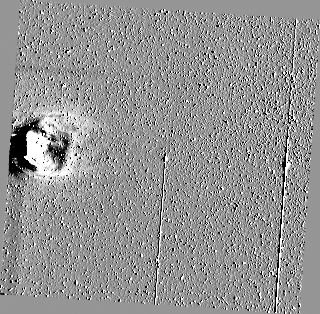
\includegraphics[interpolate=true,width=1.066667in,height=1.046667in]{plots/secchi_fov-img1.png}}%
\end{pgfscope}%
\begin{pgfscope}%
\pgfpathrectangle{\pgfqpoint{0.582966in}{0.478438in}}{\pgfqpoint{4.482034in}{2.877093in}}%
\pgfusepath{clip}%
\pgfsetbuttcap%
\pgfsetmiterjoin%
\pgfsetlinewidth{1.003750pt}%
\definecolor{currentstroke}{rgb}{0.000000,0.000000,0.000000}%
\pgfsetstrokecolor{currentstroke}%
\pgfsetdash{}{0pt}%
\pgfpathmoveto{\pgfqpoint{0.944714in}{1.480627in}}%
\pgfpathlineto{\pgfqpoint{2.009720in}{1.480627in}}%
\pgfpathlineto{\pgfqpoint{2.009720in}{2.527109in}}%
\pgfpathlineto{\pgfqpoint{0.944714in}{2.527109in}}%
\pgfpathclose%
\pgfusepath{stroke}%
\end{pgfscope}%
\begin{pgfscope}%
\definecolor{textcolor}{rgb}{0.000000,0.000000,0.000000}%
\pgfsetstrokecolor{textcolor}%
\pgfsetfillcolor{textcolor}%
\pgftext[x=1.043525in,y=1.579438in,left,base]{\color{textcolor}\rmfamily\fontsize{12.000000}{14.400000}\bfseries\selectfont HI1}%
\end{pgfscope}%
\begin{pgfscope}%
\pgfpathrectangle{\pgfqpoint{0.582966in}{0.478438in}}{\pgfqpoint{4.482034in}{2.877093in}}%
\pgfusepath{clip}%
\pgfsetbuttcap%
\pgfsetmiterjoin%
\pgfsetlinewidth{1.003750pt}%
\definecolor{currentstroke}{rgb}{0.000000,0.000000,0.000000}%
\pgfsetstrokecolor{currentstroke}%
\pgfsetdash{}{0pt}%
\pgfpathmoveto{\pgfqpoint{1.901498in}{1.915773in}}%
\pgfpathcurveto{\pgfqpoint{1.914601in}{1.915773in}}{\pgfqpoint{1.927168in}{1.920979in}}{\pgfqpoint{1.936433in}{1.930244in}}%
\pgfpathcurveto{\pgfqpoint{1.945698in}{1.939509in}}{\pgfqpoint{1.950904in}{1.952076in}}{\pgfqpoint{1.950904in}{1.965179in}}%
\pgfpathcurveto{\pgfqpoint{1.950904in}{1.978281in}}{\pgfqpoint{1.945698in}{1.990849in}}{\pgfqpoint{1.936433in}{2.000114in}}%
\pgfpathcurveto{\pgfqpoint{1.927168in}{2.009378in}}{\pgfqpoint{1.914601in}{2.014584in}}{\pgfqpoint{1.901498in}{2.014584in}}%
\pgfpathcurveto{\pgfqpoint{1.888396in}{2.014584in}}{\pgfqpoint{1.875828in}{2.009378in}}{\pgfqpoint{1.866563in}{2.000114in}}%
\pgfpathcurveto{\pgfqpoint{1.857299in}{1.990849in}}{\pgfqpoint{1.852093in}{1.978281in}}{\pgfqpoint{1.852093in}{1.965179in}}%
\pgfpathcurveto{\pgfqpoint{1.852093in}{1.952076in}}{\pgfqpoint{1.857299in}{1.939509in}}{\pgfqpoint{1.866563in}{1.930244in}}%
\pgfpathcurveto{\pgfqpoint{1.875828in}{1.920979in}}{\pgfqpoint{1.888396in}{1.915773in}}{\pgfqpoint{1.901498in}{1.915773in}}%
\pgfpathclose%
\pgfusepath{stroke}%
\end{pgfscope}%
\begin{pgfscope}%
\pgfpathrectangle{\pgfqpoint{0.582966in}{0.478438in}}{\pgfqpoint{4.482034in}{2.877093in}}%
\pgfusepath{clip}%
\pgfsetbuttcap%
\pgfsetmiterjoin%
\pgfsetlinewidth{1.003750pt}%
\definecolor{currentstroke}{rgb}{0.000000,0.000000,0.000000}%
\pgfsetstrokecolor{currentstroke}%
\pgfsetdash{}{0pt}%
\pgfpathmoveto{\pgfqpoint{1.498857in}{1.942865in}}%
\pgfpathcurveto{\pgfqpoint{1.511960in}{1.942865in}}{\pgfqpoint{1.524527in}{1.948071in}}{\pgfqpoint{1.533792in}{1.957336in}}%
\pgfpathcurveto{\pgfqpoint{1.543057in}{1.966601in}}{\pgfqpoint{1.548263in}{1.979168in}}{\pgfqpoint{1.548263in}{1.992271in}}%
\pgfpathcurveto{\pgfqpoint{1.548263in}{2.005373in}}{\pgfqpoint{1.543057in}{2.017941in}}{\pgfqpoint{1.533792in}{2.027206in}}%
\pgfpathcurveto{\pgfqpoint{1.524527in}{2.036470in}}{\pgfqpoint{1.511960in}{2.041676in}}{\pgfqpoint{1.498857in}{2.041676in}}%
\pgfpathcurveto{\pgfqpoint{1.485755in}{2.041676in}}{\pgfqpoint{1.473187in}{2.036470in}}{\pgfqpoint{1.463922in}{2.027206in}}%
\pgfpathcurveto{\pgfqpoint{1.454658in}{2.017941in}}{\pgfqpoint{1.449452in}{2.005373in}}{\pgfqpoint{1.449452in}{1.992271in}}%
\pgfpathcurveto{\pgfqpoint{1.449452in}{1.979168in}}{\pgfqpoint{1.454658in}{1.966601in}}{\pgfqpoint{1.463922in}{1.957336in}}%
\pgfpathcurveto{\pgfqpoint{1.473187in}{1.948071in}}{\pgfqpoint{1.485755in}{1.942865in}}{\pgfqpoint{1.498857in}{1.942865in}}%
\pgfpathclose%
\pgfusepath{stroke}%
\end{pgfscope}%
\begin{pgfscope}%
\pgfpathrectangle{\pgfqpoint{0.582966in}{0.478438in}}{\pgfqpoint{4.482034in}{2.877093in}}%
\pgfusepath{clip}%
\pgfsetbuttcap%
\pgfsetmiterjoin%
\pgfsetlinewidth{1.003750pt}%
\definecolor{currentstroke}{rgb}{0.000000,0.000000,0.000000}%
\pgfsetstrokecolor{currentstroke}%
\pgfsetdash{}{0pt}%
\pgfpathmoveto{\pgfqpoint{3.163965in}{2.033916in}}%
\pgfpathcurveto{\pgfqpoint{3.177068in}{2.033916in}}{\pgfqpoint{3.189635in}{2.039122in}}{\pgfqpoint{3.198900in}{2.048386in}}%
\pgfpathcurveto{\pgfqpoint{3.208165in}{2.057651in}}{\pgfqpoint{3.213371in}{2.070219in}}{\pgfqpoint{3.213371in}{2.083321in}}%
\pgfpathcurveto{\pgfqpoint{3.213371in}{2.096424in}}{\pgfqpoint{3.208165in}{2.108991in}}{\pgfqpoint{3.198900in}{2.118256in}}%
\pgfpathcurveto{\pgfqpoint{3.189635in}{2.127521in}}{\pgfqpoint{3.177068in}{2.132727in}}{\pgfqpoint{3.163965in}{2.132727in}}%
\pgfpathcurveto{\pgfqpoint{3.150863in}{2.132727in}}{\pgfqpoint{3.138295in}{2.127521in}}{\pgfqpoint{3.129030in}{2.118256in}}%
\pgfpathcurveto{\pgfqpoint{3.119766in}{2.108991in}}{\pgfqpoint{3.114560in}{2.096424in}}{\pgfqpoint{3.114560in}{2.083321in}}%
\pgfpathcurveto{\pgfqpoint{3.114560in}{2.070219in}}{\pgfqpoint{3.119766in}{2.057651in}}{\pgfqpoint{3.129030in}{2.048386in}}%
\pgfpathcurveto{\pgfqpoint{3.138295in}{2.039122in}}{\pgfqpoint{3.150863in}{2.033916in}}{\pgfqpoint{3.163965in}{2.033916in}}%
\pgfpathclose%
\pgfusepath{stroke}%
\end{pgfscope}%
\begin{pgfscope}%
\pgfpathrectangle{\pgfqpoint{0.582966in}{0.478438in}}{\pgfqpoint{4.482034in}{2.877093in}}%
\pgfusepath{clip}%
\pgfsetbuttcap%
\pgfsetmiterjoin%
\pgfsetlinewidth{1.003750pt}%
\definecolor{currentstroke}{rgb}{0.000000,0.000000,0.000000}%
\pgfsetstrokecolor{currentstroke}%
\pgfsetdash{}{0pt}%
\pgfpathmoveto{\pgfqpoint{3.416141in}{1.913435in}}%
\pgfpathcurveto{\pgfqpoint{3.429243in}{1.913435in}}{\pgfqpoint{3.441811in}{1.918640in}}{\pgfqpoint{3.451075in}{1.927905in}}%
\pgfpathcurveto{\pgfqpoint{3.460340in}{1.937170in}}{\pgfqpoint{3.465546in}{1.949738in}}{\pgfqpoint{3.465546in}{1.962840in}}%
\pgfpathcurveto{\pgfqpoint{3.465546in}{1.975943in}}{\pgfqpoint{3.460340in}{1.988510in}}{\pgfqpoint{3.451075in}{1.997775in}}%
\pgfpathcurveto{\pgfqpoint{3.441811in}{2.007040in}}{\pgfqpoint{3.429243in}{2.012245in}}{\pgfqpoint{3.416141in}{2.012245in}}%
\pgfpathcurveto{\pgfqpoint{3.403038in}{2.012245in}}{\pgfqpoint{3.390470in}{2.007040in}}{\pgfqpoint{3.381206in}{1.997775in}}%
\pgfpathcurveto{\pgfqpoint{3.371941in}{1.988510in}}{\pgfqpoint{3.366735in}{1.975943in}}{\pgfqpoint{3.366735in}{1.962840in}}%
\pgfpathcurveto{\pgfqpoint{3.366735in}{1.949738in}}{\pgfqpoint{3.371941in}{1.937170in}}{\pgfqpoint{3.381206in}{1.927905in}}%
\pgfpathcurveto{\pgfqpoint{3.390470in}{1.918640in}}{\pgfqpoint{3.403038in}{1.913435in}}{\pgfqpoint{3.416141in}{1.913435in}}%
\pgfpathclose%
\pgfusepath{stroke}%
\end{pgfscope}%
\begin{pgfscope}%
\pgfsetbuttcap%
\pgfsetmiterjoin%
\definecolor{currentfill}{rgb}{1.000000,1.000000,1.000000}%
\pgfsetfillcolor{currentfill}%
\pgfsetlinewidth{1.003750pt}%
\definecolor{currentstroke}{rgb}{0.000000,0.000000,0.000000}%
\pgfsetstrokecolor{currentstroke}%
\pgfsetdash{}{0pt}%
\pgfpathmoveto{\pgfqpoint{1.689276in}{1.715221in}}%
\pgfpathlineto{\pgfqpoint{2.113721in}{1.715221in}}%
\pgfpathlineto{\pgfqpoint{2.113721in}{1.869443in}}%
\pgfpathlineto{\pgfqpoint{1.689276in}{1.869443in}}%
\pgfpathclose%
\pgfusepath{stroke,fill}%
\end{pgfscope}%
\begin{pgfscope}%
\definecolor{textcolor}{rgb}{0.000000,0.000000,0.000000}%
\pgfsetstrokecolor{textcolor}%
\pgfsetfillcolor{textcolor}%
\pgftext[x=1.901498in,y=1.841665in,,top]{\color{textcolor}\rmfamily\fontsize{8.000000}{9.600000}\selectfont Jupiter}%
\end{pgfscope}%
\begin{pgfscope}%
\pgfsetbuttcap%
\pgfsetmiterjoin%
\definecolor{currentfill}{rgb}{1.000000,1.000000,1.000000}%
\pgfsetfillcolor{currentfill}%
\pgfsetlinewidth{1.003750pt}%
\definecolor{currentstroke}{rgb}{0.000000,0.000000,0.000000}%
\pgfsetstrokecolor{currentstroke}%
\pgfsetdash{}{0pt}%
\pgfpathmoveto{\pgfqpoint{1.297302in}{2.088006in}}%
\pgfpathlineto{\pgfqpoint{1.700413in}{2.088006in}}%
\pgfpathlineto{\pgfqpoint{1.700413in}{2.242228in}}%
\pgfpathlineto{\pgfqpoint{1.297302in}{2.242228in}}%
\pgfpathclose%
\pgfusepath{stroke,fill}%
\end{pgfscope}%
\begin{pgfscope}%
\definecolor{textcolor}{rgb}{0.000000,0.000000,0.000000}%
\pgfsetstrokecolor{textcolor}%
\pgfsetfillcolor{textcolor}%
\pgftext[x=1.498857in,y=2.115784in,,bottom]{\color{textcolor}\rmfamily\fontsize{8.000000}{9.600000}\selectfont Saturn}%
\end{pgfscope}%
\begin{pgfscope}%
\pgfsetbuttcap%
\pgfsetmiterjoin%
\definecolor{currentfill}{rgb}{1.000000,1.000000,1.000000}%
\pgfsetfillcolor{currentfill}%
\pgfsetlinewidth{1.003750pt}%
\definecolor{currentstroke}{rgb}{0.000000,0.000000,0.000000}%
\pgfsetstrokecolor{currentstroke}%
\pgfsetdash{}{0pt}%
\pgfpathmoveto{\pgfqpoint{2.983521in}{2.179057in}}%
\pgfpathlineto{\pgfqpoint{3.344410in}{2.179057in}}%
\pgfpathlineto{\pgfqpoint{3.344410in}{2.333279in}}%
\pgfpathlineto{\pgfqpoint{2.983521in}{2.333279in}}%
\pgfpathclose%
\pgfusepath{stroke,fill}%
\end{pgfscope}%
\begin{pgfscope}%
\definecolor{textcolor}{rgb}{0.000000,0.000000,0.000000}%
\pgfsetstrokecolor{textcolor}%
\pgfsetfillcolor{textcolor}%
\pgftext[x=3.163965in,y=2.206835in,,bottom]{\color{textcolor}\rmfamily\fontsize{8.000000}{9.600000}\selectfont Venus}%
\end{pgfscope}%
\begin{pgfscope}%
\pgfsetbuttcap%
\pgfsetmiterjoin%
\definecolor{currentfill}{rgb}{1.000000,1.000000,1.000000}%
\pgfsetfillcolor{currentfill}%
\pgfsetlinewidth{1.003750pt}%
\definecolor{currentstroke}{rgb}{0.000000,0.000000,0.000000}%
\pgfsetstrokecolor{currentstroke}%
\pgfsetdash{}{0pt}%
\pgfpathmoveto{\pgfqpoint{3.239974in}{1.712882in}}%
\pgfpathlineto{\pgfqpoint{3.592307in}{1.712882in}}%
\pgfpathlineto{\pgfqpoint{3.592307in}{1.867104in}}%
\pgfpathlineto{\pgfqpoint{3.239974in}{1.867104in}}%
\pgfpathclose%
\pgfusepath{stroke,fill}%
\end{pgfscope}%
\begin{pgfscope}%
\definecolor{textcolor}{rgb}{0.000000,0.000000,0.000000}%
\pgfsetstrokecolor{textcolor}%
\pgfsetfillcolor{textcolor}%
\pgftext[x=3.416141in,y=1.839327in,,top]{\color{textcolor}\rmfamily\fontsize{8.000000}{9.600000}\selectfont Earth}%
\end{pgfscope}%
\begin{pgfscope}%
\pgfpathrectangle{\pgfqpoint{0.582966in}{0.478438in}}{\pgfqpoint{4.482034in}{2.877093in}}%
\pgfusepath{clip}%
\pgfsys@transformshift{0.583333in}{1.846667in}%
\pgftext[left,bottom]{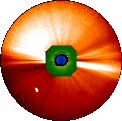
\includegraphics[interpolate=true,width=0.413333in,height=0.413333in]{plots/secchi_fov-img2.png}}%
\end{pgfscope}%
\end{pgfpicture}%
\makeatother%
\endgroup%

%     \caption[Fields of view of the \acs{STEREO} \acs{SECCHI} telescopes]{Composite image demonstrating the fields of view of the \ac{STEREO} \ac{SECCHI} telescopes EUVI, COR1, COR2 (blue, green and red areas on the left side), and HI1 and HI2. \ac{HI} images are shown as running difference images, while COR and EUVI are direct images. This image features the April 15, 2020 \ac{CME}, some planets as well as the Milky Way (diagonal band across the HI2 image).}
%     \label{fig:secchifov}
% \end{figure}

% \acp{CME} appear in the \ac{HI} telescopes due to Thomson scattering: Sunlight is scattered by free electrons in the solar wind plasma, and regions of enhanced density, such as \acp{CME} and the shocks driven by them, appear as brighter structures in the images. To make these transients more clearly visible, long exposure times on the order of 20 minutes to 1 hour are needed, and difference images are often used to further highlight the moving structures. In theory, the \SI{88.7}{\degree} field of view would allow the \acp{HI} to track \acp{CME} all the way out to Earth under most conditions. However, in practice, the \ac{CME} structures become more faint during the propagation as their density and velocity decreases. Also, \acp{CME} not directed towards Earth are not always covered by \ac{HI}, as these may also occur on the opposite side of the Sun (e.g. the left side of \autoref{fig:secchifov}).

% To routinely reconstruct the trajectories of \acp{CME} in the \ac{HI} observations, the 2D images are typically transformed into so-called J-maps, a technique which was originally developed by \citet{Sheeley-1999-JMap} and first applied to \ac{STEREO}-\ac{HI} data by \citet{Rouillard-2008-JMap}
% and \citet{Davies-2009}: After subtraction of backgrounds and the calculation of running difference images, a 1D slice is extracted from each \ac{HI} image in the time period of interest, usually close to the ecliptic plane. For each consecutive point in time, these slices are then rotated by \SI{90}{\degree} and concatenated into a new 2D plot, where time is on the x axis and the heliographic longitude, which in this case is named the \textit{elongation angle} $\epsilon$, is on the y axis. Moving structures, such as \ac{CME} or shock fronts, then appear as bright streaks in the J-map, which extend from the bottom (low elongation) out to larger elongations (see \autoref{subfig:jmap} for an example). Depending on the \ac{CME} direction and the evolution of its velocity, these structures can often resemble a (rotated) letter J, hence the corresponding naming of this type of plot. This is not the case in the example in \autoref{subfig:jmap}, as this slow \ac{CME} propagates at a nearly constant speed and produces a more or less straight line in the J-map.
% By tracing the structures in the J-map images, the time-elongation profile $\epsilon(t)$ can then easily be reconstructed.

% The more challenging part is to use this measurement to calculate the actual CME trajectory, i.e. the time profile of the radial distance $r(t)$ from the Sun. To solve this problem unambiguously, some assumptions need to be made, as the Thomson-scattered \ac{HI} image accumulates the electron density along the line of sight, which contains points at different heliospheric longitudes and radial distances. This means that the geometric shape of the \ac{CME} needs to be known to derive the position of the apex from the images. Multiple techniques have been developed to address this issue in different ways, starting with single-spacecraft approaches that also need to make assumptions about the CME longitude \citep{Howard-2006-PointP,Kahler-2007-FixedPhi,Lugaz-2009-HarmonicMean,Davies-2012-SSE}, followed by approaches that take into account the measurements from both \ac{STEREO} spacecraft at the same time to triangulate the CME location \citep{Liu-2010a-triangulation,Liu-2010b-triangulation,Lugaz-2010-TAS,Davies-2013-SSSE}. Of course, the latter can only be used for events observed by both spacecraft simultaneously, before the loss of connection to \ac{STEREO}-B in 2014. A detailed overview of these reconstruction methods and the corresponding mathematical expressions was given in Section 3.3.2 of \citet{Forstner-2018-masterthesis}.
% The single-spacecraft reconstruction methods are also summarized in Section 2.3 and Figure 2 of \citet{Forstner-2019}, which is reprinted in \autoref{chp:arrival_times} of this thesis.

% The \ac{HELCATS}\footnote{\url{https://www.helcats-fp7.eu/}} has systematically cataloged and analyzed all CMEs detected by the \ac{STEREO}-\ac{HI} telescopes and provides these data on their website. This database will serve as the basis for most \ac{HI}-related studies in this thesis. As an example, the images and J-map provided by \ac{HELCATS} for the April 15, 2020 CME observed by \ac{STEREO}-A are shown in \autoref{fig:hi_example}. The corresponding data and reconstruction results can be found under the ID \texttt{HCME\_A\_\_20200415\_01} in the \ac{HELCATS} catalogs.

% \begin{figure}
% 	\centering
% 	\subfloat[Direct image]{
% 		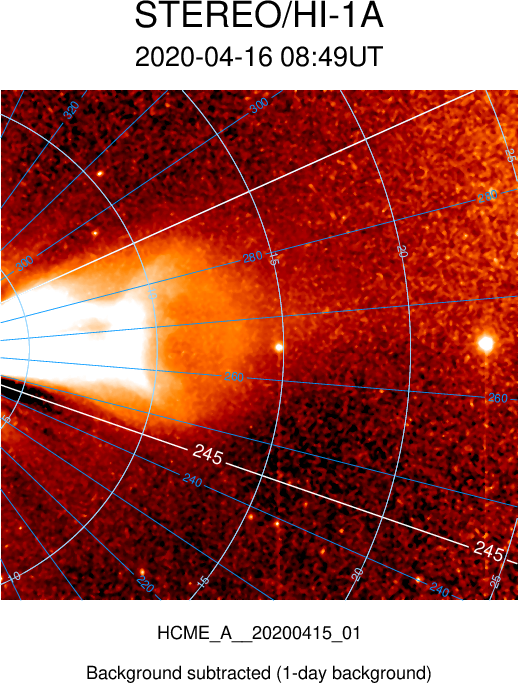
\includegraphics[width=0.4\textwidth]{images/HCME_A__20200415_01.png}
% 	}
% 	\subfloat[Running difference image]{
% 		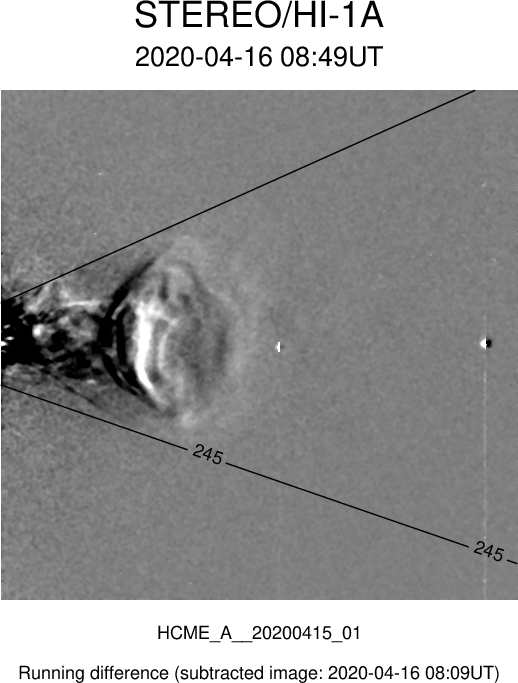
\includegraphics[width=0.4\textwidth]{images/HCME_A__20200415_01_diff.png}
% 	}\\
% 	\subfloat[J-map]{
% 		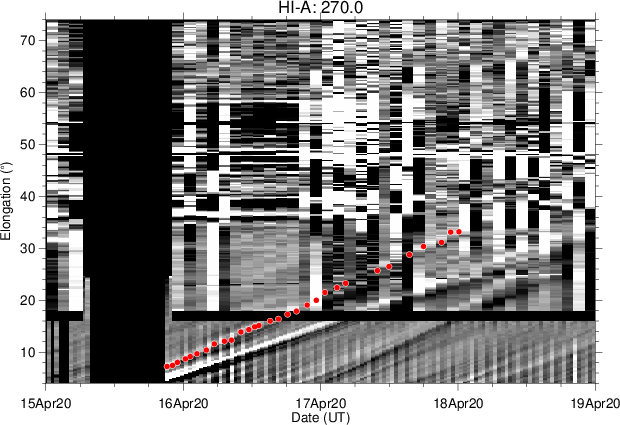
\includegraphics[width=0.8\textwidth]{images/HCME_A__20200415_01_jmap.png}
% 		\label{subfig:jmap}
% 	}
% 	\caption[\acs{STEREO}-A \acs{HI} images of the April 15, 2020 CME]{\ac{STEREO}-A \ac{HI} images of the April 15, 2020 \ac{CME} generated by the \ac{HELCATS} project. In the J-map, the \ac{CME} trajectory was marked with red dots.}
% 	\label{fig:hi_example}
%\end{figure}



\chapter{Studies of ICME arrival times at 1 AU and Mars using Forbush decreases}
\label{chp:arrival_times}

\TODO{Summary of the publications}

The following article is reproduced from \textcite{Forstner-2018} with permission from Journal of Geophysical Research: Space Physics, \copyright American Geophysical Union:\\

\noindent\pubcite{Forstner-2018}\\
\strut\hfill Own contribution: 90\%

\newpage
\newcounter{includepdfpageJGREighteen}

\addtocounter{subsection}{1}
\setcounter{subsubsection}{1} 
\phantomsection
\addcontentsline{toc}{subsection}{\arabic{chapter}.\arabic{section}.\arabic{subsection} Using Forbush Decreases to Derive the Transit Time of ICMEs Propagating from 1 AU to Mars (Publication JGR--Space Physics 2018)}
%
\phantomsection
\addcontentsline{toc}{subsubsection}{\arabic{chapter}.\arabic{section}.\arabic{subsection}.\arabic{subsubsection} Introduction}
\label{sec:paper_forstner2018}
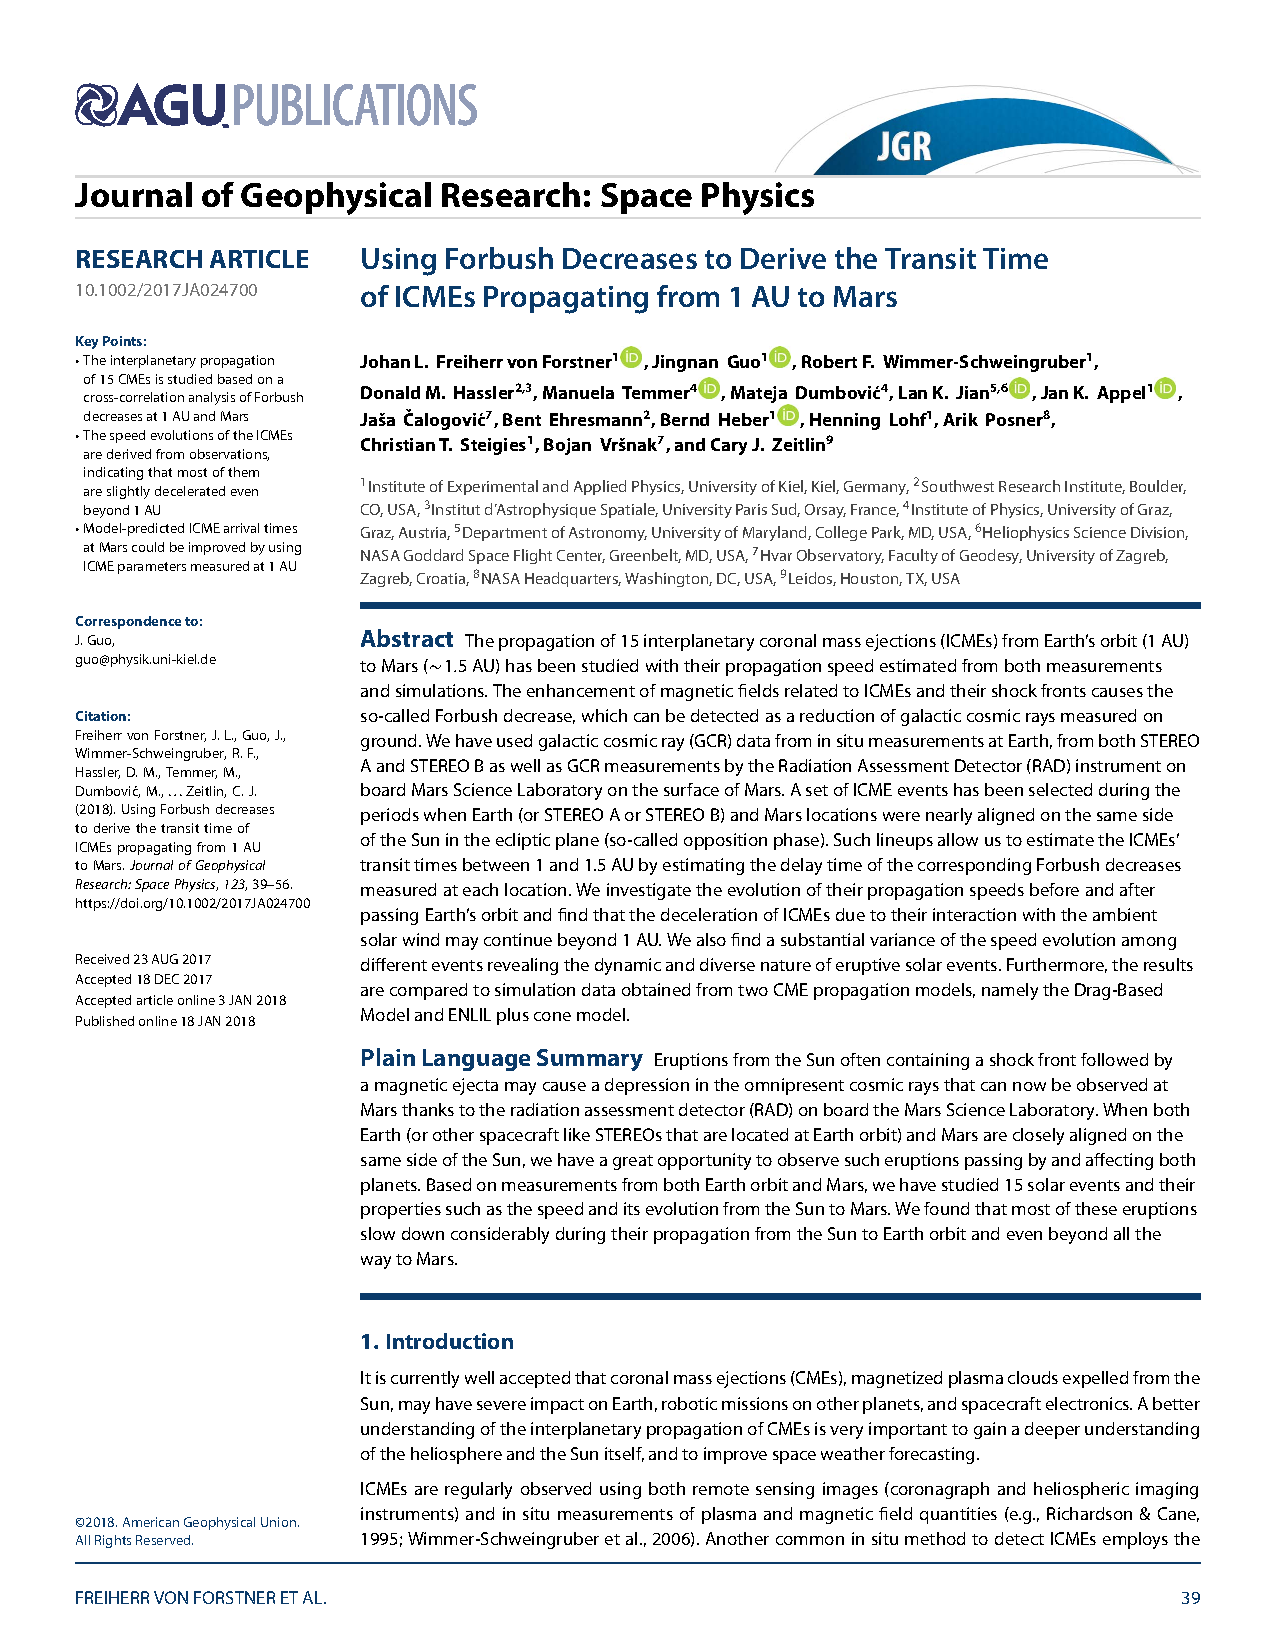
\includepdf[pages={1-2}, link, linkname=paper_forstner2018, scale=.9, pagecommand={\refstepcounter{includepdfpageJGREighteen}\label{paper_forstner2018.\theincludepdfpageJGREighteen}}]{publications/Forstner_et_al-2018-JGRSpace.pdf}
%
\addtocounter{subsubsection}{1} 
\phantomsection
\addcontentsline{toc}{subsubsection}{\arabic{chapter}.\arabic{section}.\arabic{subsection}.\arabic{subsubsection} Methods and Data}
\includepdf[pages={3-5}, link, linkname=paper_forstner2018, scale=.9, pagecommand={\refstepcounter{includepdfpageJGREighteen}\label{paper_forstner2018.\theincludepdfpageJGREighteen}}]{publications/Forstner_et_al-2018-JGRSpace.pdf}
%
\addtocounter{subsubsection}{1} 
\phantomsection
\addcontentsline{toc}{subsubsection}{\arabic{chapter}.\arabic{section}.\arabic{subsection}.\arabic{subsubsection} Results and Discussion}
\includepdf[pages={6-12}, link, linkname=paper_forstner2018, scale=.9, pagecommand={\refstepcounter{includepdfpageJGREighteen}\label{paper_forstner2018.\theincludepdfpageJGREighteen}}]{publications/Forstner_et_al-2018-JGRSpace.pdf}
%
\addtocounter{subsubsection}{1} 
\phantomsection
\addcontentsline{toc}{subsubsection}{\arabic{chapter}.\arabic{section}.\arabic{subsection}.\arabic{subsubsection} Conclusion}
\includepdf[pages={13}, link, linkname=paper_forstner2018, scale=.9, pagecommand={\refstepcounter{includepdfpageJGREighteen}\label{paper_forstner2018.\theincludepdfpageJGREighteen}}]{publications/Forstner_et_al-2018-JGRSpace.pdf}
%
\addtocounter{subsubsection}{1} 
\phantomsection
\addcontentsline{toc}{subsubsection}{\arabic{chapter}.\arabic{section}.\arabic{subsection}.\arabic{subsubsection} Appendix A: Cross-Correlation Analysis Plots for Each Event}
\includepdf[pages={14-16}, link, linkname=paper_forstner2018, scale=.9, pagecommand={\refstepcounter{includepdfpageJGREighteen}\label{paper_forstner2018.\theincludepdfpageJGREighteen}}]{publications/Forstner_et_al-2018-JGRSpace.pdf}
%
\addtocounter{subsubsection}{1} 
\phantomsection
\addcontentsline{toc}{subsubsection}{\arabic{chapter}.\arabic{section}.\arabic{subsection}.\arabic{subsubsection} References}
\includepdf[pages={17-18}, link, linkname=paper_forstner2018, scale=.9, pagecommand={\refstepcounter{includepdfpageJGREighteen}\label{paper_forstner2018.\theincludepdfpageJGREighteen}}]{publications/Forstner_et_al-2018-JGRSpace.pdf}

The following article is reproduced from \textcite{Forstner-2019} with permission from Space 
Weather, \copyright American Geophysical Union:\\

\noindent\pubcite{Forstner-2019}\\
\strut\hfill Own contribution: 90\%

\newpage
\newcounter{includepdfpageSWNineteen}

\addtocounter{subsection}{1}
\setcounter{subsubsection}{1} 
\phantomsection
\addcontentsline{toc}{subsection}{\arabic{chapter}.\arabic{section}.\arabic{subsection} Tracking and Validating ICMEs Propagating Toward Mars Using STEREO Heliospheric Imagers Combined With Forbush Decreases Detected by MSL/RAD (Publication Space Weather 2019)}
%
\phantomsection
\addcontentsline{toc}{subsubsection}{\arabic{chapter}.\arabic{section}.\arabic{subsection}.\arabic{subsubsection} Introduction}
\label{sec:paper_forstner2019}
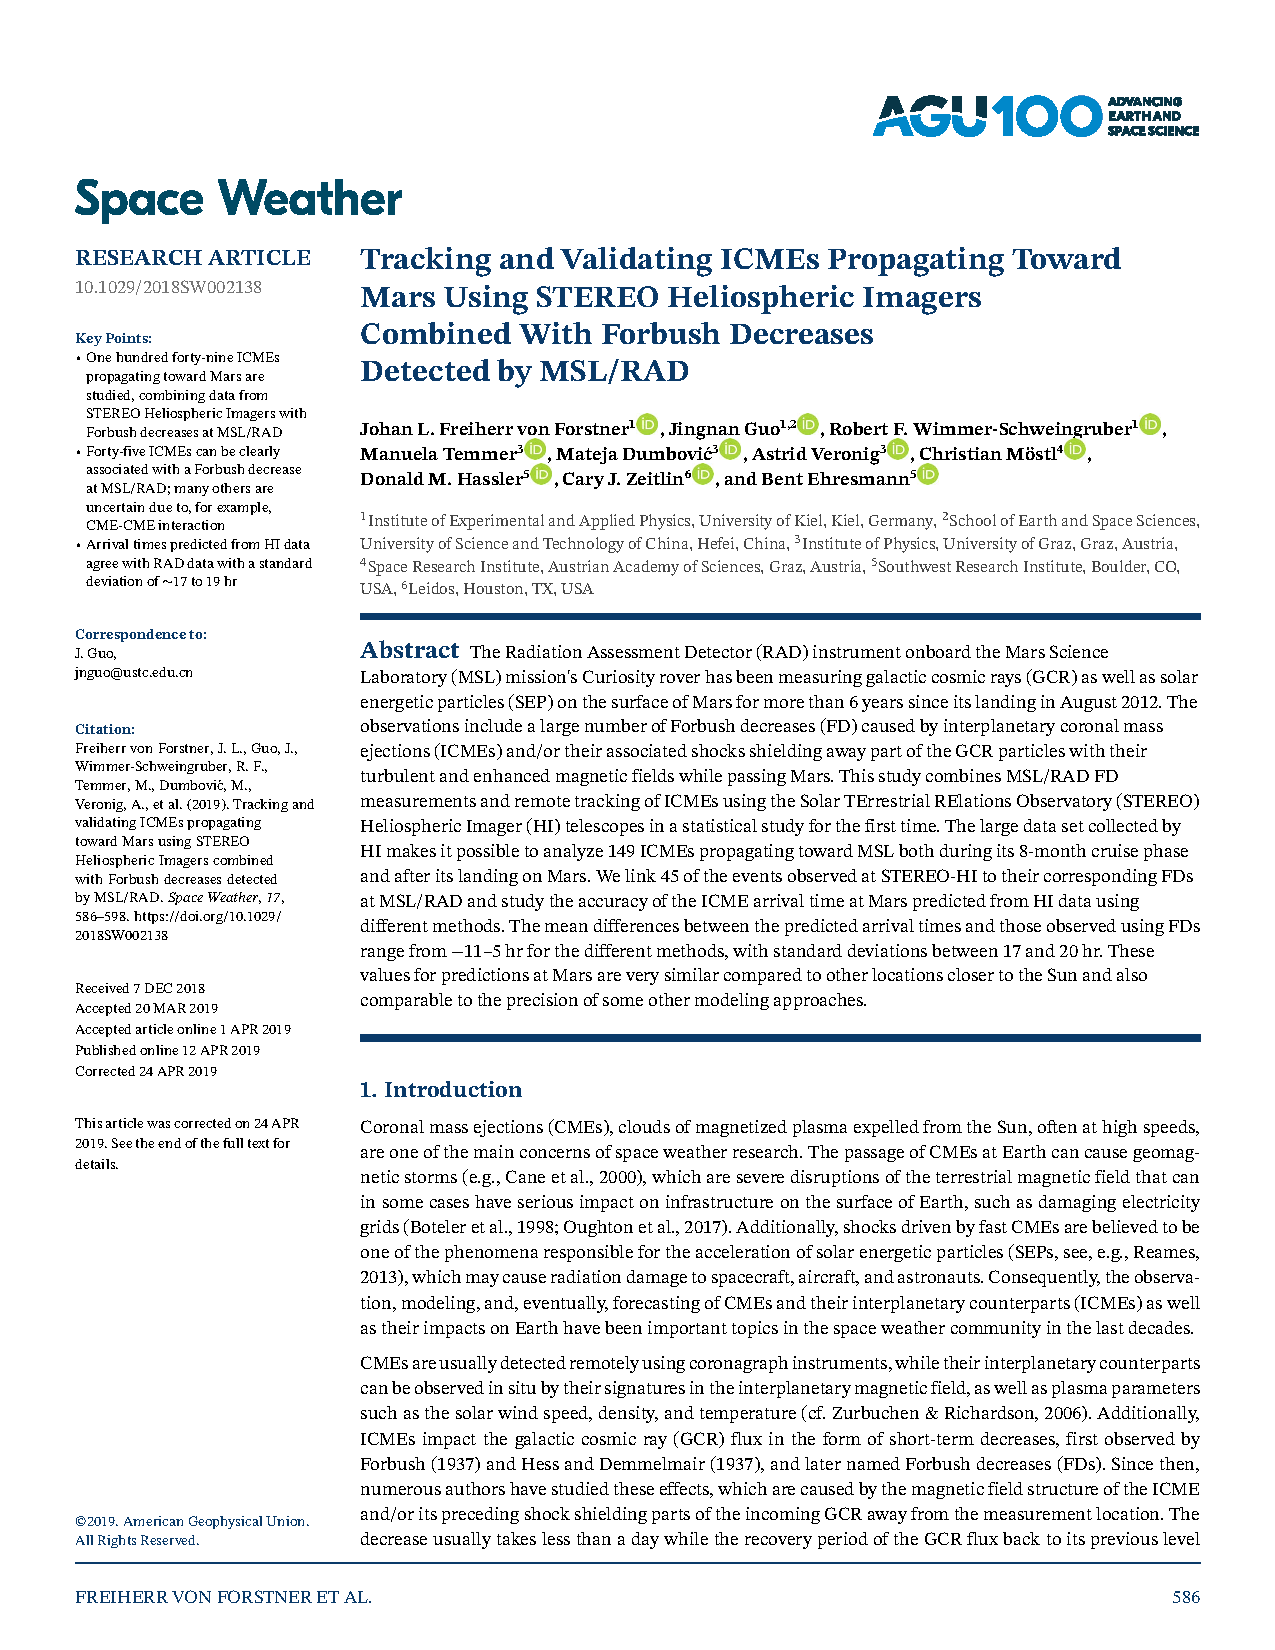
\includepdf[pages={1}, link, linkname=paper_forstner2019, scale=.95, pagecommand={\refstepcounter{includepdfpageSWNineteen}\label{paper_forstner2019.\theincludepdfpageSWNineteen}}]{publications/Forstner_et_al-2019-Space_Weather.pdf}
%
\addtocounter{subsubsection}{1} 
\phantomsection
\addcontentsline{toc}{subsubsection}{\arabic{chapter}.\arabic{section}.\arabic{subsection}.\arabic{subsubsection} Data and Methods}
\includepdf[pages={2-3}, link, linkname=paper_forstner2019, scale=.95, pagecommand={\refstepcounter{includepdfpageSWNineteen}\label{paper_forstner2019.\theincludepdfpageSWNineteen}}]{publications/Forstner_et_al-2019-Space_Weather.pdf}
%
\addtocounter{subsubsection}{1} 
\phantomsection
\addcontentsline{toc}{subsubsection}{\arabic{chapter}.\arabic{section}.\arabic{subsection}.\arabic{subsubsection} Results and Discussion}
\includepdf[pages={4-9}, link, linkname=paper_forstner2019, scale=.95, pagecommand={\refstepcounter{includepdfpageSWNineteen}\label{paper_forstner2019.\theincludepdfpageSWNineteen}}]{publications/Forstner_et_al-2019-Space_Weather.pdf}
%
\addtocounter{subsubsection}{1} 
\phantomsection
\addcontentsline{toc}{subsubsection}{\arabic{chapter}.\arabic{section}.\arabic{subsection}.\arabic{subsubsection} Conclusions and Outlook}
\includepdf[pages={10}, link, linkname=paper_forstner2019, scale=.95, pagecommand={\refstepcounter{includepdfpageSWNineteen}\label{paper_forstner2019.\theincludepdfpageSWNineteen}}]{publications/Forstner_et_al-2019-Space_Weather.pdf}
%
\addtocounter{subsubsection}{1} 
\phantomsection
\addcontentsline{toc}{subsubsection}{\arabic{chapter}.\arabic{section}.\arabic{subsection}.\arabic{subsubsection} References}
\includepdf[pages={11-13}, link, linkname=paper_forstner2019, scale=.95, pagecommand={\refstepcounter{includepdfpageSWNineteen}\label{paper_forstner2019.\theincludepdfpageSWNineteen}}]{publications/Forstner_et_al-2019-Space_Weather.pdf}

\section{Outlook}

\chapter{Comparing Forbush decrease properties at Earth and Mars}
\label{chp:fd_properties}

While in \autoref{chp:arrival_times}, \acp{FD} have mainly been used to determine the arrival time of \acp{ICME} at \SI{1}{\AU} and Mars, other properties of \acp{FD} have been neglected in these studies. However, some empirical relations between different properties of a \ac{FD} at Earth as well as between the \ac{FD} and properties of the associated \ac{ICME} are known, as shown e.g. by \citet{Belov-2008-FD,Abunin-2012-FD}. For example, there is a clear correlation between the relative \ac{FD} amplitude or the maximum decrease rate (``steepness'') with the product of the maximum solar wind speed and maximum magnetic field. This parameter $v_\text{max} \cdot B_\text{max}$ can be used to describe the intensity of the disturbance in the solar wind. The correlation is shown in Figure 8 of \citet{Belov-2008-FD} and Figure 7 of \citet{Abunin-2012-FD}.
However, solar wind plasma and magnetic field measurements at Mars are only available from the \ac{MAVEN} spacecraft since 2014, and as explained in \autoref{sec:motivation}, it does not observe the upstream solar wind continuously. So, the determination of maximum values for $B$ and $v$, which would be necessary for the validation of this relation at Mars, may be complicated for many events.

Instead, in this study, we focus on the ``inner relation'' of the two FD parameters: the relative amplitude and the maximum decrease rate. These are also known to be correlated at Earth, as seen in Figure 7 of \citet{Belov-2008-FD} and Figure 5 of \citet{Abunin-2012-FD}. We use our catalog of \acp{FD} from \citet{Forstner-2019}, as well as the larger catalog by \citet{Papaioannou-2019-FD-Earth-Mars} to reproduce this relation at Mars. Consulting the analytical \ac{FD} models, \acs{PDB} and \acs{ForbMod}, which were introduced in \autoref{sec:forbush}, it becomes possible to interpret the difference between the two observed relations as a result of the expansion of the interplanetary structures.

\TODO{Summary of the publication}

\newpage

The following article is reproduced from \textcite{Forstner-2020} from Journal of Geophysical Research: Space Physics, \copyright American Geophysical Union, under the Creative Commons CC-BY license: \ccLogo\ccAttribution\\

\pubcite{Forstner-2020}
\hfill Own contribution: 80\%

\newpage
\newcounter{includepdfpageJGRTwenty}

\addtocounter{section}{1}
\setcounter{subsection}{1} 
\phantomsection
\addcontentsline{toc}{section}{\arabic{chapter}.\arabic{section} Comparing the Properties of ICME-Induced Forbush Decreases at Earth and Mars (Publication JGR--Space Physics 2020)}
%
\phantomsection
\addcontentsline{toc}{subsection}{\arabic{chapter}.\arabic{section}.\arabic{subsection} Introduction}
\label{sec:paper_forstner2020}
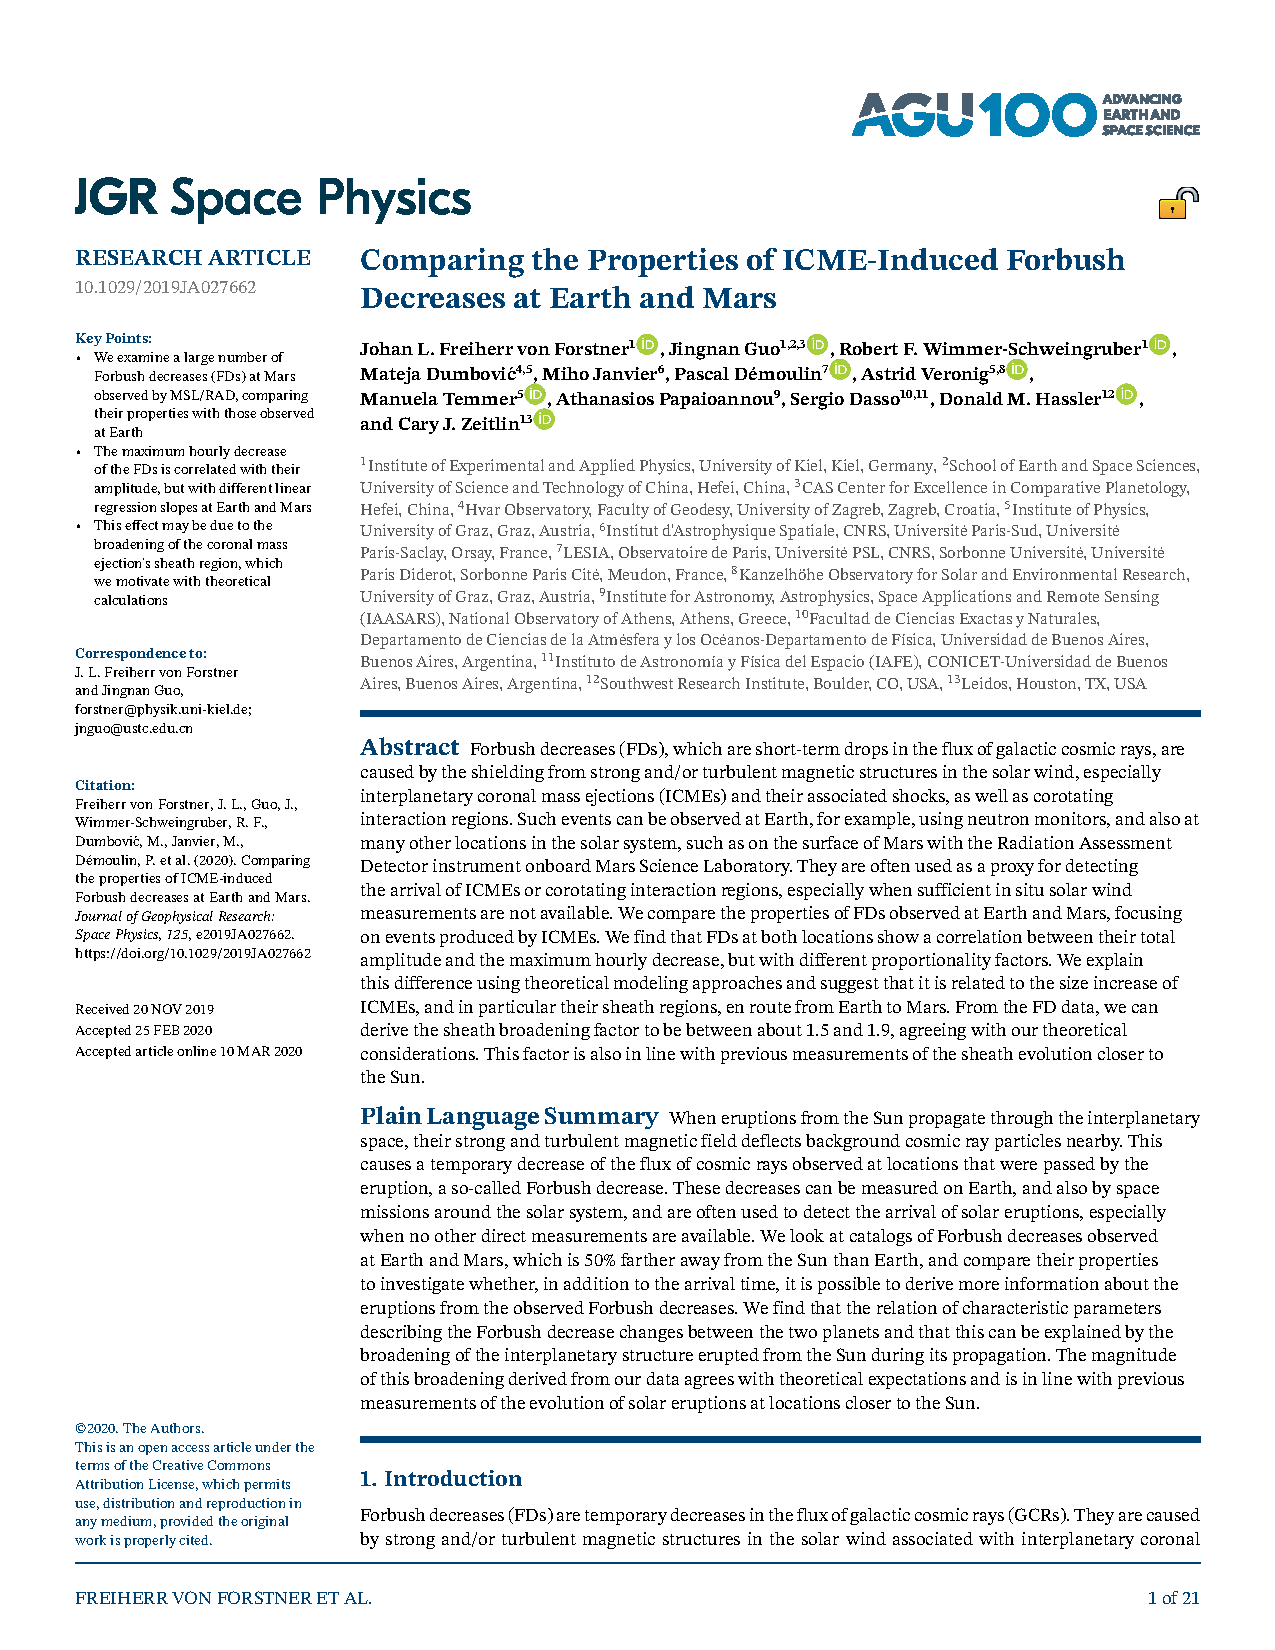
\includepdf[pages={1}, link, linkname=paper_forstner2020, scale=.95, pagecommand={\refstepcounter{includepdfpageJGRTwenty}\label{paper_forstner2020.\theincludepdfpageJGRTwenty}}]{publications/Forstner_et_al-2020-JGRSpace.pdf}
%
\addtocounter{subsection}{1} 
\phantomsection
\addcontentsline{toc}{subsection}{\arabic{chapter}.\arabic{section}.\arabic{subsection} Data Sources and Catalogs}
\includepdf[pages={2-5}, link, linkname=paper_forstner2020, scale=.95, pagecommand={\refstepcounter{includepdfpageJGRTwenty}\label{paper_forstner2020.\theincludepdfpageJGRTwenty}}]{publications/Forstner_et_al-2020-JGRSpace.pdf}
%
\addtocounter{subsection}{1} 
\phantomsection
\addcontentsline{toc}{subsection}{\arabic{chapter}.\arabic{section}.\arabic{subsection} Definitions and Methodology}
\includepdf[pages={6-7}, link, linkname=paper_forstner2020, scale=.95, pagecommand={\refstepcounter{includepdfpageJGRTwenty}\label{paper_forstner2020.\theincludepdfpageJGRTwenty}}]{publications/Forstner_et_al-2020-JGRSpace.pdf}
%
\addtocounter{subsection}{1} 
\phantomsection
\addcontentsline{toc}{subsection}{\arabic{chapter}.\arabic{section}.\arabic{subsection} Results and Discussions}
\includepdf[pages={8-16}, link, linkname=paper_forstner2020, scale=.95, pagecommand={\refstepcounter{includepdfpageJGRTwenty}\label{paper_forstner2020.\theincludepdfpageJGRTwenty}}]{publications/Forstner_et_al-2020-JGRSpace.pdf}
%
\addtocounter{subsection}{1} 
\phantomsection
\addcontentsline{toc}{subsection}{\arabic{chapter}.\arabic{section}.\arabic{subsection} Conclusions and Outlook}
%
\addtocounter{subsection}{1} 
\phantomsection
\addcontentsline{toc}{subsection}{\arabic{chapter}.\arabic{section}.\arabic{subsection} Appendix A: Location of $m_{\text{max}}$ Within the ICME Substructures}
\includepdf[pages={17-18}, link, linkname=paper_forstner2020, scale=.95, pagecommand={\refstepcounter{includepdfpageJGRTwenty}\label{paper_forstner2020.\theincludepdfpageJGRTwenty}}]{publications/Forstner_et_al-2020-JGRSpace.pdf}
%
\addtocounter{subsection}{1} 
\phantomsection
\addcontentsline{toc}{subsection}{\arabic{chapter}.\arabic{section}.\arabic{subsection} References}
\includepdf[pages={19-21}, link, linkname=paper_forstner2020, scale=.95, pagecommand={\refstepcounter{includepdfpageJGRTwenty}\label{paper_forstner2020.\theincludepdfpageJGRTwenty}}]{publications/Forstner_et_al-2020-JGRSpace.pdf}

\chapter{Major Space Weather events: The events of September 2017}
\label{chp:september_event}

Between September 4 and 10, 2017, there was a sudden increase in solar activity when an active region (number 12673, as assigned by NOAA) produced four X-class flares, including the two strongest flares of Solar Cycle 24 (X9.3 on September 6 and X8.2 on September 10).
These solar events, associated with the release of \acp{SEP} as well as the eruption of multiple fast \acp{CME}, caused a \ac{GLE} of energetic particles seen with neutron monitors on the surface of the Earth (\ac{GLE} \# 72 in the \ac{GLE} database at the University of Oulu\footnote{\url{https://gle.oulu.fi/}}) as well as with the \ac{MSL} \ac{RAD} on Mars. This makes it the first \ac{GLE} observed simultaneously on the surface of two different planets.
The \ac{SEP} event was very widespread (Earth and Mars had a longitudinal separation of $\sim$\SI{155}{\degree} at that time) and the largest \ac{GLE} seen on the surface of Mars with \ac{MSL}/\ac{RAD} so far. At Earth, the disturbances associated with the solar events caused, for example, a suppression of critical high frequency (HF) radio communications systems \citep{Frissell-2018,Bland-2018} as well as navigation satellite systems such as GPS \citep{Berdermann-2018,Sato-2019}.
These major events have been studied in great detail, and many of the articles concerning these events can be found in the special issues of \citet{SpaceWeather-2018-special-issue-September-event} as well as \citet{GRL-2018-special-issue-September-event}, where the latter is focusing on its impact on Mars.

While the September 6 flare had the stronger X-ray emission, the \ac{SEP} event associated with the later September 10 flare is the one that caused the \ac{GLE} seen at Earth and Mars, due to the better magnetic connection. Three \acp{CME} also erupted on September 9 and 10 from the same active region in similar directions ($\sim$\SI{115}{\degree} in \ac{HEE} coordinates), the last one with an extremely high speed of more than \SI{2600}{\kilo\meter\per\second}. This fast and wide \ac{CME} quickly merged with the two previous ones and formed an intense interplanetary shock. The merged eruption propagated outward quickly and was observed in situ at both Earth and Mars on September 12 and 13, respectively. While the \ac{SEP} event at Mars was still in its declining phase, the shock arrival caused a strong \ac{FD} at Mars with an amplitude of \SI{15}{\percent}, the largest \ac{FD} seen by \ac{RAD} to date. This decrease below the pre-\ac{SEP} levels was sustained over 5 days and then gradually recovered over the course of several weeks.

The following two articles \citep{Zeitlin-2018,Guo-2018} study the effects of the September 10 events on Mars as measured by \ac{MSL}/\ac{RAD} and explain these observations by modeling the \ac{SEP} event and the three \acp{CME}. \citet{Zeitlin-2018} report the dosimetric quantities measured on the Martian surface, emphasizing that the increased dose and dose equivalent rates during the \ac{GLE} on Mars are almost canceled out by the long-lasting \ac{FD} following it. Thus, in the case of a long-stay mission scenario, the increased radiation exposure due to the September event would have been insignificant for astronauts on Mars despite the 2- to 3-fold increase during the peak of the \ac{SEP} event. However, as Mars was not particularly well connected to the active region, the impact of the \ac{SEP} event could have been much larger, so this conclusion should not be generalized to all major solar events at Mars. In \citet{Guo-2018}, the propagation of the 3 \acp{CME} towards Earth and Mars is studied in more detail. The initial parameters of the \acp{CME} close to the Sun are reconstructed using \ac{GCS} fitting (see also \autoref{chp:GCS_Python}), and then the kinematics of the propagation are calculated using the \ac{DBM} (see \autoref{sec:cmes}). This is one of the first instances where \ac{DBM} is used in a \ac{CME}-\ac{CME}-interaction scenario, with one previous example being the study of \citet{Temmer-2012}. In this case, we assume a simple conservation of momentum for modeling the interaction process. The values of the drag parameter $\gamma$ were then chosen appropriately to reproduce the observed arrival times at Earth and Mars. These results are also compared to more sophisticated \ac{MHD} simulations performed for the same event.

\newpage

The following article is reproduced from \textcite{Zeitlin-2018} with permission from Geophysical Research Letters, \copyright American Geophysical Union:\\

\pubcite{Zeitlin-2018}
\hfill Own contribution: 10\%

\newpage
\newcounter{includepdfpageZeitlinEighteen}

\addtocounter{section}{1}
\setcounter{subsection}{1} 
\phantomsection
\addcontentsline{toc}{section}{\arabic{chapter}.\arabic{section} Analysis of the radiation hazard observed by RAD on the surface of Mars during the September 2017 solar particle event (Publication GRL 2018)}
%
\phantomsection
\addcontentsline{toc}{subsection}{\arabic{chapter}.\arabic{section}.\arabic{subsection} Introduction}
\label{sec:paper_zeitlin2018}
%
\addtocounter{subsection}{1} 
\phantomsection
\addcontentsline{toc}{subsection}{\arabic{chapter}.\arabic{section}.\arabic{subsection} Triggering and Data Acquisition}
%
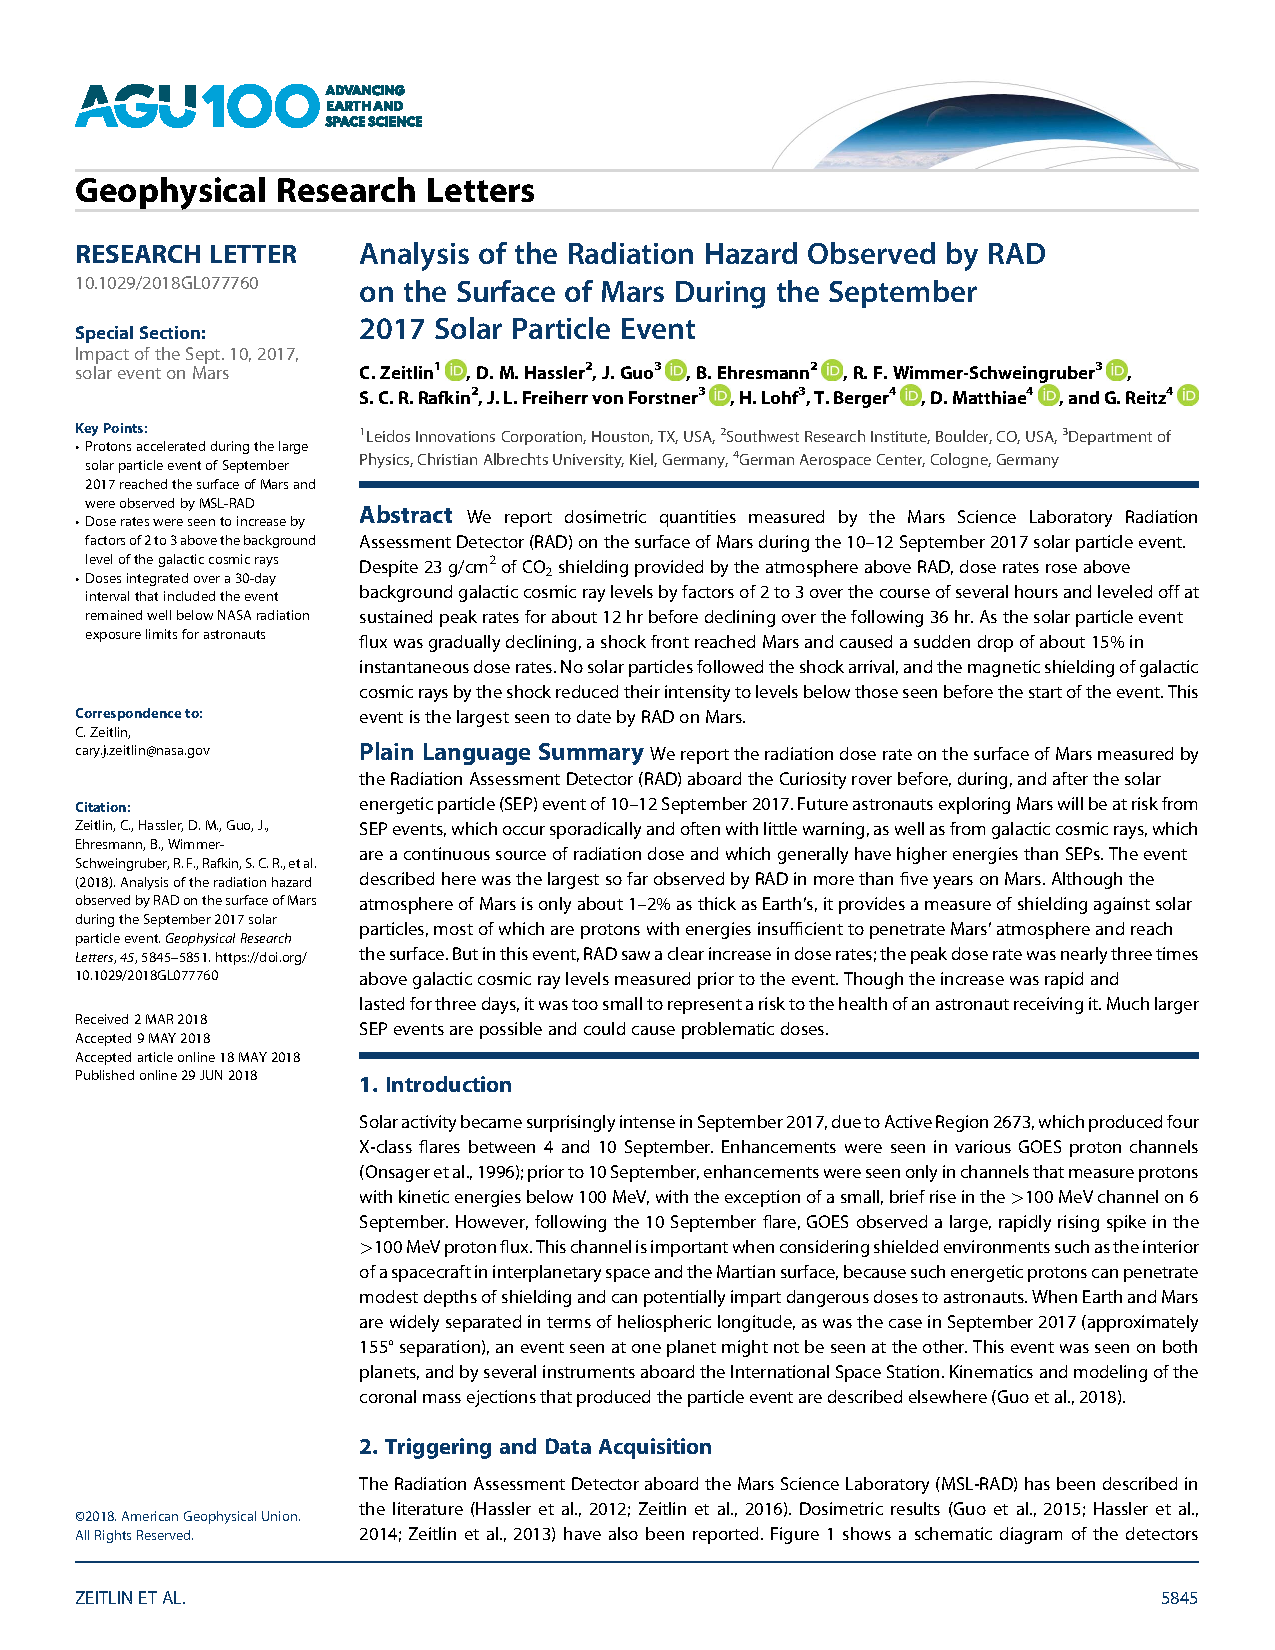
\includepdf[pages={1}, link, linkname=paper_zeitlin2018, scale=.95, pagecommand={\refstepcounter{includepdfpageZeitlinEighteen}\label{paper_zeitlin2018.\theincludepdfpageZeitlinEighteen}}]{publications/Zeitlin_et_al-2018-Geophysical_Research_Letters}
%
\addtocounter{subsection}{1} 
\phantomsection
\addcontentsline{toc}{subsection}{\arabic{chapter}.\arabic{section}.\arabic{subsection} Results}
\includepdf[pages={2-5}, link, linkname=paper_zeitlin2018, scale=.95, pagecommand={\refstepcounter{includepdfpageZeitlinEighteen}\label{paper_zeitlin2018.\theincludepdfpageZeitlinEighteen}}]{publications/Zeitlin_et_al-2018-Geophysical_Research_Letters}
%
\addtocounter{subsection}{1} 
\phantomsection
\addcontentsline{toc}{subsection}{\arabic{chapter}.\arabic{section}.\arabic{subsection} Conclusions}
\includepdf[pages={6}, link, linkname=paper_zeitlin2018, scale=.95, pagecommand={\refstepcounter{includepdfpageZeitlinEighteen}\label{paper_zeitlin2018.\theincludepdfpageZeitlinEighteen}}]{publications/Zeitlin_et_al-2018-Geophysical_Research_Letters}
%
\addtocounter{subsection}{1} 
\phantomsection
\addcontentsline{toc}{subsection}{\arabic{chapter}.\arabic{section}.\arabic{subsection} References}
\includepdf[pages={7}, link, linkname=paper_zeitlin2018, scale=.95, pagecommand={\refstepcounter{includepdfpageZeitlinEighteen}\label{paper_zeitlin2018.\theincludepdfpageZeitlinEighteen}}]{publications/Zeitlin_et_al-2018-Geophysical_Research_Letters}
\newpage

The following article is reproduced from \textcite{Guo-2018} with permission from Space Weather, \copyright American Geophysical Union:\\

\noindent
\pubcite{Guo-2018}
\hfill Own contribution: 10\%

\newpage
\newcounter{includepdfpageGuoEighteen}

\addtocounter{section}{1}
\setcounter{subsection}{1} 
\phantomsection
\addcontentsline{toc}{section}{\arabic{chapter}.\arabic{section} Modeling the Evolution and Propagation of 10 September 2017 CMEs and SEPs Arriving at Mars Constrained by Remote Sensing and In Situ Measurement (Publication Space Weather 2018)}
%
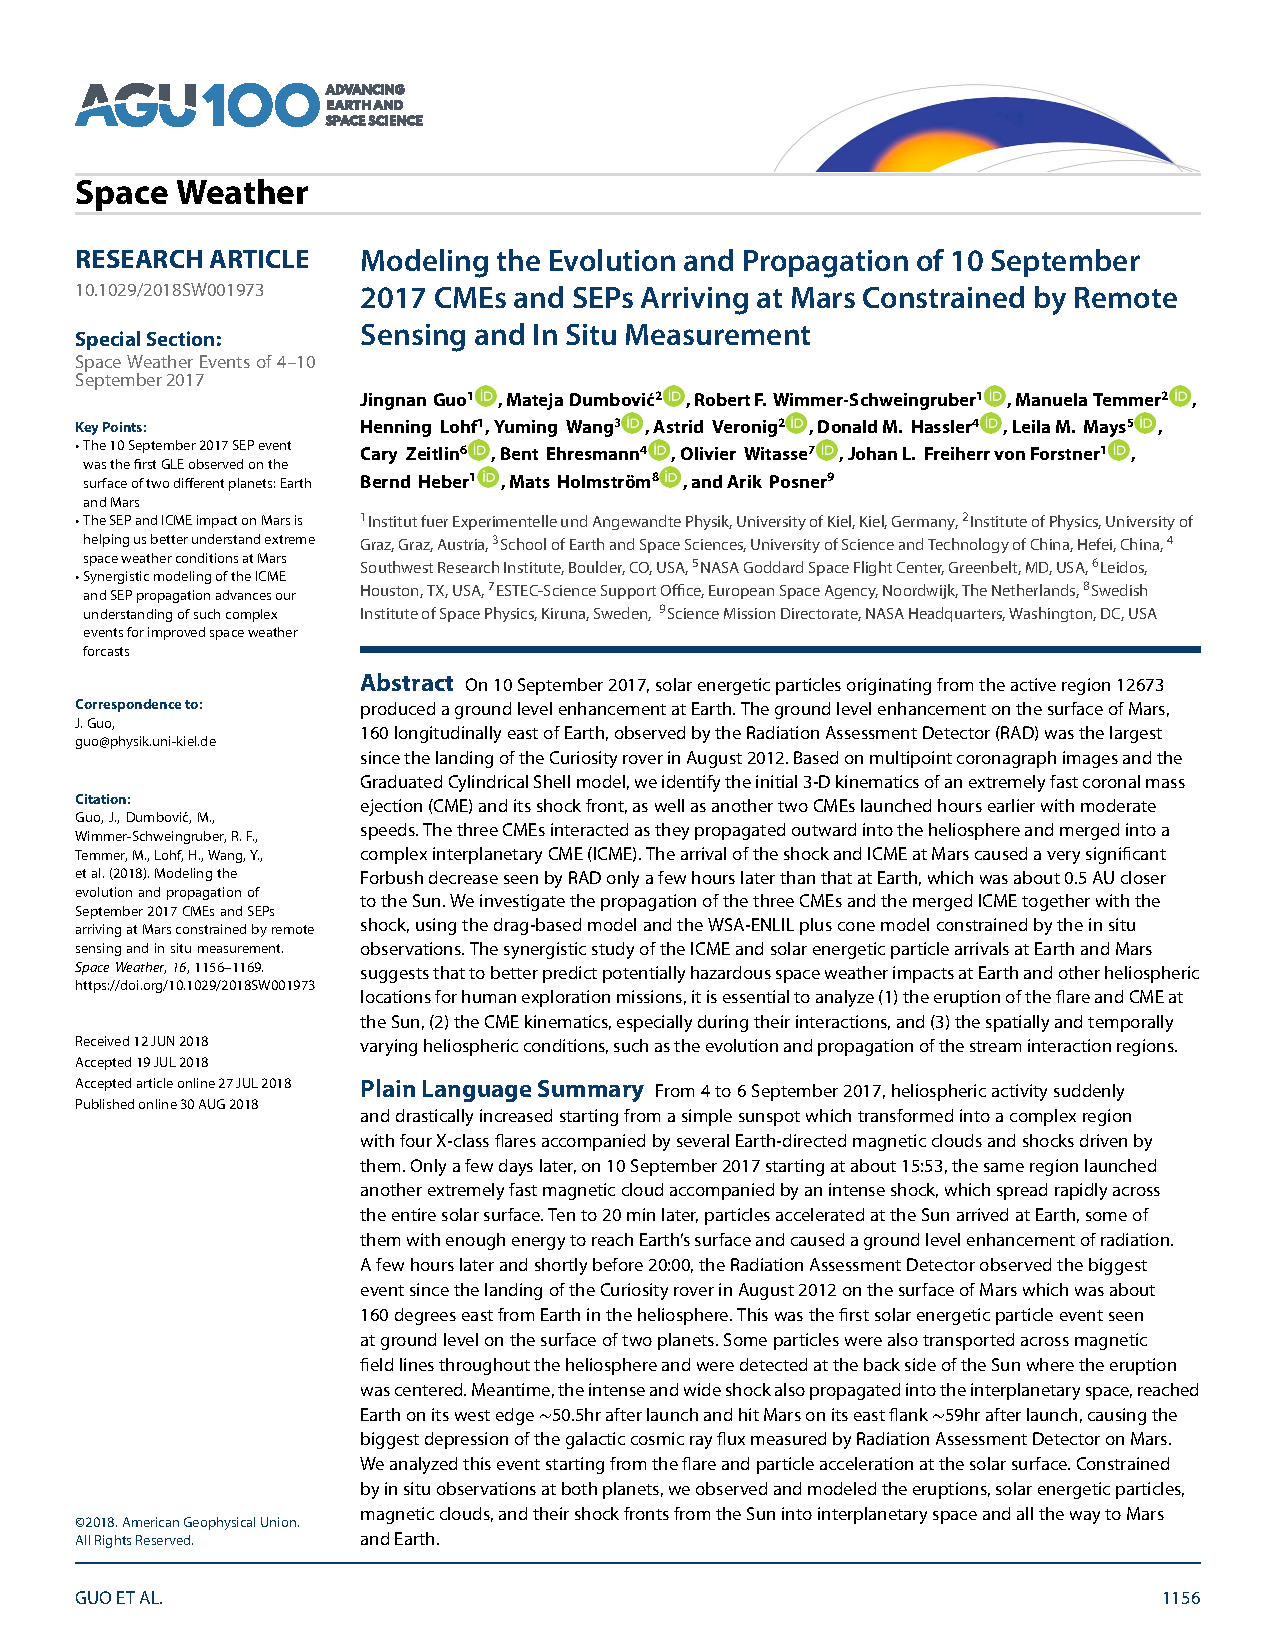
\includepdf[pages={1}, link, linkname=paper_guo2018, scale=.95, pagecommand={\refstepcounter{includepdfpageGuoEighteen}\label{paper_guo2018.\theincludepdfpageGuoEighteen}}]{publications/Guo_et_al-2018-Space_Weather}
%
\phantomsection
\addcontentsline{toc}{subsection}{\arabic{chapter}.\arabic{section}.\arabic{subsection} The Flare, CMEs, and GLE 72: Close to the Sun}
\label{sec:paper_guo2018}
%
\includepdf[pages={2-4}, link, linkname=paper_guo2018, scale=.95, pagecommand={\refstepcounter{includepdfpageGuoEighteen}\label{paper_guo2018.\theincludepdfpageGuoEighteen}}]{publications/Guo_et_al-2018-Space_Weather}
%
\addtocounter{subsection}{1} 
\phantomsection
\addcontentsline{toc}{subsection}{\arabic{chapter}.\arabic{section}.\arabic{subsection} The Interplanetary Trajectory and Interaction of Three CMEs Modeled by the DBM}
\includepdf[pages={5-6}, link, linkname=paper_guo2018, scale=.95, pagecommand={\refstepcounter{includepdfpageGuoEighteen}\label{paper_guo2018.\theincludepdfpageGuoEighteen}}]{publications/Guo_et_al-2018-Space_Weather}
%
\addtocounter{subsection}{1} 
\phantomsection
\addcontentsline{toc}{subsection}{\arabic{chapter}.\arabic{section}.\arabic{subsection} Shock Kinematics and Propagation Toward Earth and Mars: Data-Constrained DBM}
\includepdf[pages={7}, link, linkname=paper_guo2018, scale=.95, pagecommand={\refstepcounter{includepdfpageGuoEighteen}\label{paper_guo2018.\theincludepdfpageGuoEighteen}}]{publications/Guo_et_al-2018-Space_Weather}
%
\addtocounter{subsection}{1} 
\phantomsection
\addcontentsline{toc}{subsection}{\arabic{chapter}.\arabic{section}.\arabic{subsection} The Shock and ICME Arrival at Mars and Earth: Modeled Results and In Situ Observations}
\includepdf[pages={8}, link, linkname=paper_guo2018, scale=.95, pagecommand={\refstepcounter{includepdfpageGuoEighteen}\label{paper_guo2018.\theincludepdfpageGuoEighteen}}]{publications/Guo_et_al-2018-Space_Weather}
%
\addtocounter{subsection}{1} 
\phantomsection
\addcontentsline{toc}{subsection}{\arabic{chapter}.\arabic{section}.\arabic{subsection} SEPs Arriving at Earth, Mars, and STA and the Indication of the Shockand Stream Interaction Region Propagation}
\includepdf[pages={9-10}, link, linkname=paper_guo2018, scale=.95, pagecommand={\refstepcounter{includepdfpageGuoEighteen}\label{paper_guo2018.\theincludepdfpageGuoEighteen}}]{publications/Guo_et_al-2018-Space_Weather}
%
\addtocounter{subsection}{1} 
\phantomsection
\addcontentsline{toc}{subsection}{\arabic{chapter}.\arabic{section}.\arabic{subsection} Summary and Conclusion}
\includepdf[pages={11}, link, linkname=paper_guo2018, scale=.95, pagecommand={\refstepcounter{includepdfpageGuoEighteen}\label{paper_guo2018.\theincludepdfpageGuoEighteen}}]{publications/Guo_et_al-2018-Space_Weather}
%
\addtocounter{subsection}{1} 
\phantomsection
\addcontentsline{toc}{subsection}{\arabic{chapter}.\arabic{section}.\arabic{subsection} Appendix A: References of the Measurements and Databases Employed in This Study}
\includepdf[pages={12}, link, linkname=paper_guo2018, scale=.95, pagecommand={\refstepcounter{includepdfpageGuoEighteen}\label{paper_guo2018.\theincludepdfpageGuoEighteen}}]{publications/Guo_et_al-2018-Space_Weather}
%
\addtocounter{subsection}{1} 
\phantomsection
\addcontentsline{toc}{subsection}{\arabic{chapter}.\arabic{section}.\arabic{subsection} References}
\includepdf[pages={13-14}, link, linkname=paper_guo2018, scale=.95, pagecommand={\refstepcounter{includepdfpageGuoEighteen}\label{paper_guo2018.\theincludepdfpageGuoEighteen}}]{publications/Guo_et_al-2018-Space_Weather}

\chapter{Case study: First CME seen at Solar Orbiter}
\label{chp:solo}

Together with the NASA \ac{PSP} launched in August 2018, the ESA \ac{SolO} mission ushers in a new era in solar and heliospheric physics. For the first time since the 1970s, these spacecraft will approach the Sun significantly closer than the orbit of Mercury --- \ac{PSP} has already set a new record with less than \SI{0.1}{\AU} solar distance at its most recent perihelion in September 2020. On the other hand, \ac{SolO}, which was launched in February 2020, will stay far enough away from the Sun to also allow for observations through holes in its heatshield. In the extended mission phase, it is planned to incline the orbit of \ac{SolO} to also observe the poles of the Sun for the first time.

As part of the \ac{EPD} suite on \ac{SolO} \citep{RodriguezPacheco-2019-EPD}, the \acl{HET}\acused{HET} (\acs{HET}, \autoref{sec:solohet}) has been successfully commissioned and is providing some first measurements of high-energy charged particles. While a few \ac{SEP} events in the first 10 months of the mission did extend to the energies covered by \ac{HET} ($\gtrsim\SI{6}{\mega\electronvolt\per nuc}$ ions and $>\SI{450}{\kilo\electronvolt}$ electrons), \ac{HET} spent most of the time observing the \ac{GCR} background, as the Sun was very quiet during this time. As discussed in \autoref{sec:solohet}, \ac{HET} is also able to resolve short-term variations of the \ac{GCR} with some of its data products, and consequently, some \acp{FD} have been measured, which were caused by \acp{CME} and \acp{CIR} that passed \ac{SolO} during its first orbit.

The first \ac{FD} seen at \ac{SolO} caused by a \ac{CME} on April 19, 2020 is especially interesting, as it is a multispacecraft event that was also observed near Earth one day later during a close longitudinal alignment and with a radial separation of \SI{0.2}{\AU}. The \ac{CME} was also seen at the BepiColombo spacecraft that was still close to Earth at this time, and may also have hit Venus, though no observations at Venus are available due to the loss of contact with the Venus Express spacecraft in 2014. Furthermore, \ac{STEREO}-A was in a perfect position to provide a side view of the \ac{CME} with its remote sensing instruments. In the following publication, which was submitted to \textit{Astronomy \& Astrophysics} in November 2020, we describe the capabilities of \ac{HET}, present the \ac{FD} observed at \ac{SolO} and the corresponding observations near Earth, and investigate the radial evolution of the \ac{CME} by applying \acs{ForbMod} (see \autoref{sec:forbush}) to this event. Another study of the same event, focusing on the magnetic field observations, has also been submitted by Emma E. Davies of Imperial College, and both will be published in the ``Solar Orbiter First Results'' special issue of \textit{A\&A} in 2021.

In the process of this study, a new implementation of the \ac{GCS} model \citep{Thernisien-2011-GCS} was developed. Details about this software can be found in \autoref{chp:GCS_Python}.

The following article is reproduced from \textcite{Forstner-2021-SolO} with permission from Astronomy \& Astrophysics, \copyright  ESO:\\

\noindent
\pubcite{Forstner-2021-SolO}
\hfill Own contribution: 80\%

\newpage
\newcounter{includepdfpageAATwentyOne}

\addtocounter{section}{1}
\setcounter{subsection}{1} 
\phantomsection
\addcontentsline{toc}{section}{\arabic{chapter}.\arabic{section} Radial Evolution of the April 2020 Stealth Coronal Mass Ejection between 0.8 and 1 AU: A Comparison of Forbush Decreases at Solar Orbiter and Earth (Publication A\&A 2021)}
%
\phantomsection
\addcontentsline{toc}{subsection}{\arabic{chapter}.\arabic{section}.\arabic{subsection} Introduction}
\label{sec:paper_forstner2021}
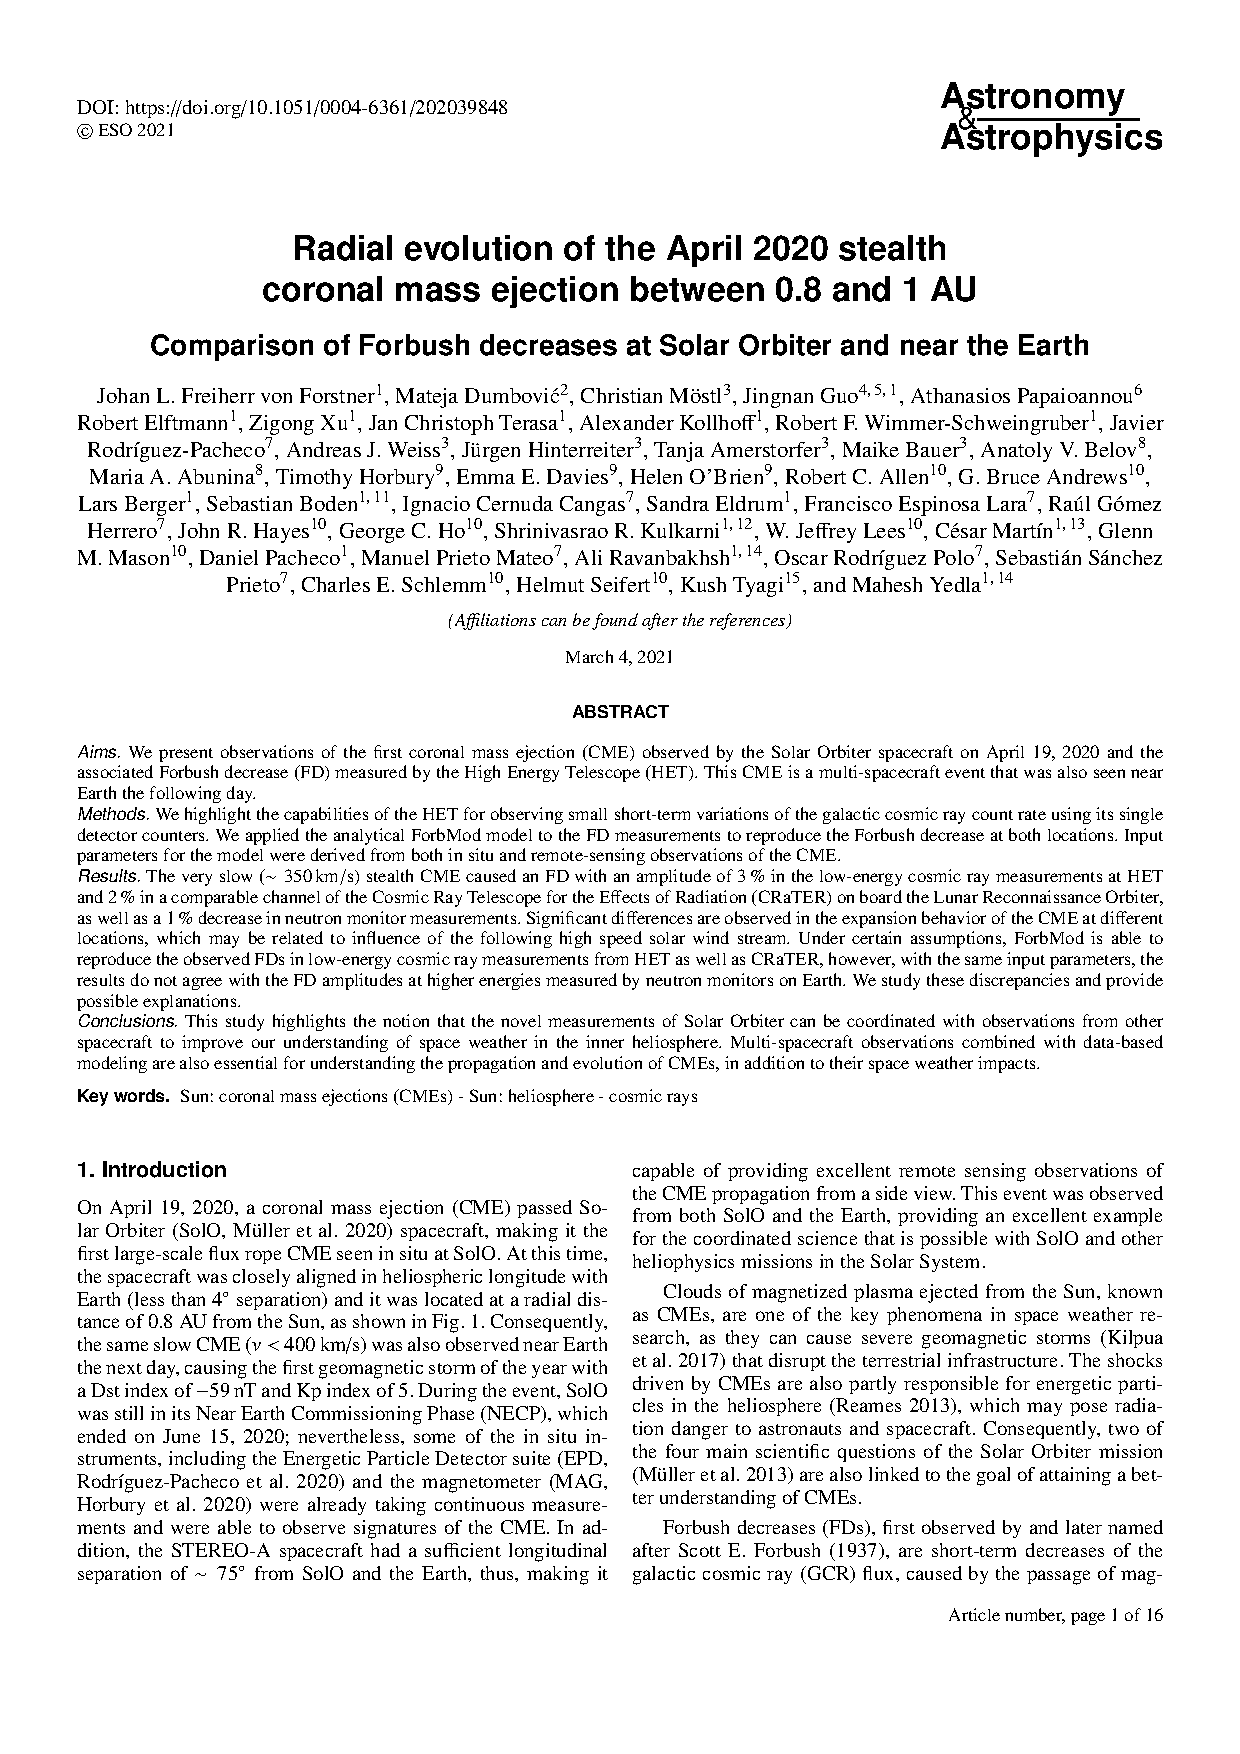
\includepdf[pages={1}, link, linkname=paper_forstner2021, scale=.95, pagecommand={\refstepcounter{includepdfpageAATwentyOne}\label{paper_forstner2021.\theincludepdfpageAATwentyOne}}]{publications/Forstner_et_al-2021-AandA.pdf}
%
\addtocounter{subsection}{1} 
\phantomsection
\addcontentsline{toc}{subsection}{\arabic{chapter}.\arabic{section}.\arabic{subsection} Data Sources}
\includepdf[pages={2-4}, link, linkname=paper_forstner2021, scale=.95, pagecommand={\refstepcounter{includepdfpageAATwentyOne}\label{paper_forstner2021.\theincludepdfpageAATwentyOne}}]{publications/Forstner_et_al-2021-AandA.pdf}
%
\addtocounter{subsection}{1} 
\phantomsection
\addcontentsline{toc}{subsection}{\arabic{chapter}.\arabic{section}.\arabic{subsection} Methods}
%
\addtocounter{subsection}{1} 
\phantomsection
\addcontentsline{toc}{subsection}{\arabic{chapter}.\arabic{section}.\arabic{subsection} Results}
\includepdf[pages={5-10}, link, linkname=paper_forstner2021, scale=.95, pagecommand={\refstepcounter{includepdfpageAATwentyOne}\label{paper_forstner2021.\theincludepdfpageAATwentyOne}}]{publications/Forstner_et_al-2021-AandA.pdf}
%
\addtocounter{subsection}{1} 
\phantomsection
\addcontentsline{toc}{subsection}{\arabic{chapter}.\arabic{section}.\arabic{subsection} Discussion and conclusions}
\includepdf[pages={11-13}, link, linkname=paper_forstner2021, scale=.95, pagecommand={\refstepcounter{includepdfpageAATwentyOne}\label{paper_forstner2021.\theincludepdfpageAATwentyOne}}]{publications/Forstner_et_al-2021-AandA.pdf}
%
\addtocounter{subsection}{1} 
\phantomsection
\addcontentsline{toc}{subsection}{\arabic{chapter}.\arabic{section}.\arabic{subsection} References}
\includepdf[pages={14-15}, link, linkname=paper_forstner2021, scale=.95, pagecommand={\refstepcounter{includepdfpageAATwentyOne}\label{paper_forstner2021.\theincludepdfpageAATwentyOne}}]{publications/Forstner_et_al-2021-AandA.pdf}
%


% ********************************************************************
% Backmatter
%*******************************************************
\newpage
\markboth{}{\thepage}
\cleardoublepage
\phantomsection
\addcontentsline{toc}{chapter}{Bibliography}

\printbibliography

\cleardoublepage
%*******************************************************
% Acknowledgements
%*******************************************************
\refstepcounter{dummy}
\pdfbookmark[0]{Acknowledgements}{Acknowledgements}
\chapter*{Acknowledgements}

At this point, I want to express my gratitude to everyone who has played an important role during the course of my Ph.D. Their assistance, guidance, and support have been invaluable over the past five years. Without their help, I would not be where I am now.

First of all, I would like to thank my supervisor, Prof. Robert F. Wimmer-Schweingruber, for giving me the opportunity to join the group and work on the exciting projects - Chang'E-4/LND and SolO/EPD. He supported me in publishing these results in scientific journals and presenting them at multiple international conferences. I enjoyed discussing scientific topics with him. Those discussions inspired me and made me more productive.

I am also grateful to Prof. Jingnan Guo, who recommended me to Robert five years ago. She guided and helped me a lot on the LND projects. I hope I can have opportunities to continue our collaborations in the future. Besides, I would like to thank Prof. Dressing Nina, who provided valuable instructions and comments on the SEP paper of LND. She kindly wrote me a strong reference letter for me for the postdoc application of Caltech. That recommendation must be one of the key factors that help me to be selected from multiple candidates.

Furthermore, many thanks are given to my lovely colleagues working on LND and SOLO projects and in the Kiel group. Firstly, I would like to thank my officemate Dr. Lars Berger, for his patience and kindness every time I asked him basic and stupid questions. These discussions with him were one of the best moments that I enjoyed most. Despite that, I would like to show special thanks to him for his encouragement during finishing my thesis in the last two months. By the way, I still can not enjoy your heavy metal music. 
Secondly, I would like to show my appreciation to Dr. Verena Heidrich-Meisner, Dr. Patrick K\"{u}hl, and Dr. Marquardt Johannes for their proofreading of this thesis. They provided valuable suggestions and vastly improved the thesis.
Next, I want to express my appreciation to my colleagues in the Kiel group for their help. They are the future Ph.D., Alexander Kollhoff, Chaoran Gu, Salman Khaksarighiri, Kr\"{o}hnke Henning, as well as Dr. Daniel Pacheco, Dr. Liu Yang, Dr. Johan von Forstner, Dr. Jia Yu, and Henning Lohf.

I also want to thank my friends in Kiel, Jinru He, Lei Shao, Xuenan Li, and Xiuming Sun, who have always supported me, taken care of me, and helped me survive the tough COVID times. I remember the time that we enjoyed the fried chicken wings and played Catan all night until the following day. Thanks to those tough times, they made me stronger and more confident.

In the end, I would like to thank my parents - Aifang Wang and Fazhen Xu - for their understanding and support during my studies. 
Specifically, I would like to express my deepest love and gratitude to my wife, Zhenlin Zhu. She always has my back, and I am so lucky to have her in my life.


Further acknowledgments to the online tools for thesis writing and proofreading, including but not limited to Chatgpt, Grammarly, NotionAI, and DeepL. They are mighty in correcting grammar mistakes.
 

% At this point, I would like to thank everyone who supported me during the course of my Ph.D. studies and my work on MSL/RAD, Chang'E 4 LND, as well as Solar Orbiter EPD.

% First of all, I am grateful to my supervisor, Prof. Robert Wimmer-Schweingruber for the opportunity to work on these exciting projects, and his helpful advice. He also made it possible that these results could be published in scientific journals and presented at many international conferences. Sincere thanks also to Prof. Jingnan Guo, who supported my work since my bachelor's thesis, and who I wish all the best for her new position in China.

% Furthermore, thanks to all my colleagues in the three mission teams for their continued support and helpful discussions, including Zigong Xu, Alexander Kollhoff, and my officemate Christoph Terasa for the productive and enjoyable collaboration, e.g. on low- and high-level software for the Solar Orbiter mission, which will hopefully facilitate the EPD data analysis in the Kiel team for years to come, and to the rest of the Extraterrestrial Physics group at Kiel University. I also thank the group of Manuela Temmer and Astrid Veronig at the University of Graz and Mateja Dumbović at Hvar Observatory with whom I worked in close collaboration for many of the Forbush decrease studies, and who I enjoyed meeting regularly at the conferences in Vienna, Hvar and San Francisco.

% I additionally want to thank the bachelor and master students who supported my work during their Hiwi positions, Charlotte Büschel and Niklas Lundt, and three secondary school students, Joana Wanger, Lukas Abegg and Markus Arndt, who contributed to the data sets used in my studies during their internships in the ET group.

% I would like to thank Anne Fischer as well as Hanna Giese and Knud Schröter for their very thorough proofreading of this thesis and valuable suggestions, and my parents Kristina and Michael and my brother Julius for their moral support. 

% Last but not least, the data analysis presented in this thesis, the typesetting of the thesis itself and the generation of most of the figures were made possible by a number of open source software projects, including, but not limited to, the ones acknowledged below:

% \begin{refsection}[software.bib]
%   \nocite{*}
%   \newrefcontext[sorting=none]
%   \printbibliography[heading=none]
% \end{refsection}

\cleardoublepage
\appendix
\chapter{Isotropic simulation of the High Energy Telescope with the Solar Orbiter spacecraft model}
\label{chp:HETSimulation}

To simulate the response of the High Energy Telescope (HET, \autoref{sec:solohet}), part of the Energetic Particle Detector \citep[EPD][]{RodriguezPacheco-2019-EPD} onboard Solar Orbiter (SolO), for an isotropic radiation field, a simulation using the GEometry And Tracking 4 \citep[Geant4][]{Agostinelli-2003} was performed. GEANT4 is a software toolkit developed at CERN for Monte Carlo simulations of the interaction of particles with matter, and is widely used in many different fields. A Geant4 simulation typically requires the definition of a particle source (e.g. a particle beam, a surface or volume source), a model of the geometry and materials of the experimental setup, and one or more sensitive detectors in which particle hits are detected. A so-called ``physics list'' describes all possible interaction processes and their probabilities, from which Geant4 then chooses stochastically for each simulated particle. As a result, the trajectory of each particle and the detected particles in each detector can be stored and used processed to calculate e.g. the response function of a particle detector.

This simulation builds on top of the work by \citet{Elftmann-2020-PhD}, who simulated the nominal data products of HET with Geant4. In this case, particles were simulated only from a circular source in front of the A detector \citet[Figure 5.1]{Elftmann-2020-PhD}, which fills the nominal field of view (FOV) of HET. However, particles entering HET from outside its FOV may also play a role for certain data products, especially for single-detector counters, which are sensitive to particles entering the telescope from all directions (e.g., through the housing). These counters were used by \citet{Forstner-2021-SolO} to observe Forbush decreases with HET. Thus, it makes sense to simulate the HET detector in an isotropic particle flux to model its response to Galactic Cosmic Rays (GCRs), and this will be done in \autoref{sec:isotropic_sim}.

For an isotropic particle flux, it is also important to take into account the Solar Orbiter spacecraft that HET is mounted on. This is less relevant for the nominal FOV, as the HET telescopes are oriented so that their openings do not point towards the spacecraft body (i.e. tangential to an edge of the body). But for single detector counters, particles coming from the solid angle covered by the spacecraft can be shielded away, or may generate secondaries that are then detected within HET. This will be investigated in \autoref{sec:spacecraft_model}.

\section{Isotropic simulation of HET}
\label{sec:isotropic_sim}

For the isotropic simulation, the geometric model of the HET instrument and its electronics box were reused from the simulation by \citet{Elftmann-2020-PhD}, so the reader is referred to this work for further details about its definition. The simulation setup was also very similar to \citet{Elftmann-2020-PhD}, using Geant4 version 10.1.2 with the pre-defined general-purpose physics list \texttt{QGSP\_BERT}, and a power law spectrum for the energy-dependent intensity $I$ of the input particles:
\begin{equation}
I(E) \sim E^{-1}
\end{equation}
This makes it possible to simulate the same number of particles in each primary energy bin when the bins are logarithmically spaced. Only protons between \SI{5}{\mega\electronvolt} and \SI{100}{\giga\electronvolt} were simulated as input particles in this case, as other species were neglected in the modeling approach of \citet{Forstner-2021-SolO}. Still, all secondary particles generated by these primary protons are taken into account in the output of simulation. Of course, other primary species such as electrons and heavy ions can be simulated in a similar fashion in the future.

In contrast to the circular planar source surface used by \citet{Elftmann-2020-PhD}, a spherical source with a radius of \SI{15}{\centi\meter} (large enough to surround HET and its electronics box) was defined, and particles were injected following a cosine-law angular distribution. This represents an isotropic flux entering HET from all sides.
The simulation was run for \num{5e8} particles, and $\sim\num{1.6e7}$ particle hits (primary or secondary) were registered in the HET detectors.

\section{The spacecraft model}
\label{sec:spacecraft_model}

To simulate how the interaction of GCR particles with the Solar Orbiter spacecraft affects the HET measurements, the spacecraft needs to be included into the Geant4 simulation. Accurately modeling a spacecraft is notoriously difficult, as it consists of numerous components and information about their exact shape and composition is not always readily available. Thus, simulations taking into account spacecraft effects often need to make many assumptions and drastically simplify the geometry of the spacecraft (see e.g. \citet{Appel-2018-PhD,Appel-2018} for a similar simulation of the Mars Science Laboratory rover).

In the case of Solar Orbiter, ESA has provided a computer-aided design (CAD) model of the spacecraft that can serve as a reference for simulations (D. Müller, 2020, priv. comm.). This file (\texttt{dpl7a1\_bulk.bdf}) is provided in the NASTRAN BDF format
and contains the 3D geometry of the spacecraft, including material properties such as the density. Using the freeware software \textit{FEX}\footnote{\url{http://www.f-e-x.com/}}, it is possible to inspect the model and measure the dimensions and total mass of certain structures.

As shown in \autoref{fig:solo_spacecraft_model}, the model accurately represents the major structures of the SolO spacecraft, such as the main body, the solar panels, the heat shield, the instrument boom and various communications and radio wave antennae. However, not all parts are modeled in detail: Many small structures, such as the scientific payload and electronics within the spacecraft body, are replaced with mass points that are attached to the model (shown as colored tetrahedra in the image), and thus no information about their extent and materials are provided. In addition, some parts of the spacecraft are constructed using composite materials, such as honeycomb structures instead of solid Aluminium --- in these cases, the material properties given in the CAD file do not include the correct density, but are instead set to zero. Thus, the total mass of the spacecraft according to the CAD file is \SI{1202}{\kilogram}, which is significantly less than the total launch mass off $\sim\SI{1800}{\kilo\gram}$, or $\sim\SI{1600}{\kilo\gram}$ without fuel \citep{Mueller-2020-SolO}.

\begin{figure}
	\centering
	\includegraphics[width=0.7\linewidth]{images/solo_spacecraft_model}
	\caption[Density model of the Solar Orbiter spacecraft]{Density model of the Solar Orbiter spacecraft as supplied by ESA. Colored tetrahedra correspond to mass points that are inserted into the model as a replacement for structures whose geometry is not modeled (e.g. scientific payload).}
	\label{fig:solo_spacecraft_model}
\end{figure}

An automated conversion from the CAD file to a Geant4-compatible model (GDML) is not easily possible and would also not be very meaningful due to the shortcomings of the CAD model described above.
As a first step towards implementing the spacecraft model in Geant4, I have therefore simply measured the dimensions of the main box-shaped spacecraft body in the CAD file and created a corresponding box in Geant4. To estimate the mass of this box, the following estimations are made: 
The total mass of the two solar panels in the CAD file is \SI{110}{\kilo\gram}, so the main spacecraft body (without solar panels) has a mass of $\sim\SI{1100}{\kilogram} + \SI{600}{\kilogram} = \SI{1700}{\kilogram}$ (adding the \SI{400}{\kilogram} of mass that is ``missing'' in the CAD file \SI{200}{\kilogram} of fuel). This value is used as the mass of the box in the Geant4 model.
For the material of the box, we assume that the mass is equally distributed throughout the box, with \SI{200}{\kilogram} of hydrazine fuel, and the remaining mass split 50:50 between electronics components and aluminium (\SI{750}{\kilogram} each). Electronics were modeled using the PCB material taken from \citet{Appel-2018,Appel-2018-PhD}.
The dimensions and materials used are summarized in \autoref{tab:solo_spacecraft_gdml}.

\begin{table}
    \begin{tabular}{rp{6cm}}
        \toprule
        \multicolumn{2}{c}{\textbf{SolO spacecraft body}}                   \\
        \midrule
        X dimension & \SI{1812}{\milli\meter}                \\
        Y dimension & \SI{1461}{\milli\meter}                \\
        Z dimension & \SI{2200}{\milli\meter}                \\
        Mass        & \SI{1700}{\kilogram}                   \\
        Density     & \SI{291.89}{\kilogram\per\cubic\meter} \\
        Composition & \SI{12}{\percent} Hydrazine (N$_2$H$_4$) \newline \SI{44}{\percent} PCB material (see right table) \newline \SI{44}{\percent} Aluminium Alloy (same as HET housing) \\
        \bottomrule
    \end{tabular}
    \hspace{1cm}
    \begin{tabular}{rr}
    	\toprule
    	\multicolumn{2}{c}{\textbf{PCB material}} \\ \midrule
    	Cu      & \SI{20}{\percent}     \\
    	SiO$_2$ & \SI{15}{\percent}     \\
    	PET     & \SI{9.9}{\percent}    \\
    	PP      & \SI{4.8}{\percent}    \\
    	Al      & \SI{2}{\percent}      \\
    	Pb      & \SI{2}{\percent}      \\
    	Ni      & \SI{2}{\percent}      \\
    	Fe      & \SI{8}{\percent}      \\
    	Sn      & \SI{4}{\percent}      \\
    	Mg      & \SI{30}{\percent}     \\ \bottomrule
    \end{tabular}
    \caption{Details of the spacecraft model used for the HET simulation. The left table shows the dimensions and composition of the box-shaped spacecraft body, while the right table shows the PCB material taken from \citet{Appel-2018,Appel-2018-PhD}.}
    \label{tab:solo_spacecraft_gdml}
\end{table}

HET was then positioned next to the spacecraft body, at a location derived from the position of the corresponding mass point of HET 1 in the CAD file, and with the correct orientation relative to the Sun. As both HET 1 and HET 2 are located at an edge of the spacecraft body, the difference between the positions of HET 1 and HET 2 is not expected to be significant for an isotropic radiation field --- but of course, this may be verified with another simulation in the future. As a source, a cube of edge length \SI{260}{\centi\meter}, which surrounds the spacecraft body and the HET sensor was used, again with a cosine-law distribution of particles injected from its surface.

To speed up future simulations, the spacecraft model may also be converted into spherical shells of equivalent column density that are placed around the HET sensor. In this case, the source size could be significantly reduced and thus the fraction of simulated particles that reach HET would increase. The simulation results with the actual spacecraft geometry can then be used to validate this approach.

\section{Analysis of the simulation results}

For the study by \citet{Forstner-2021-SolO}, the 

\cleardoublepage
\chapter{Implementation of the Graduated Cylindrical Shell model in Python}
\label{chp:GCS_Python}

The Graduated Cylindrical Shell model \citep[GCS,][]{Thernisien-2006-GCS,Thernisien-2011-GCS} is an empirical model that is commonly used to represent the three-dimensional structure of flux rope CMEs near the Sun. It defines a croissant-like 3D shape with conical legs whose ends are anchored to the center of the Sun, as shown in \autoref{fig:gcs_schematic}.

\begin{figure}
    \begin{tikzpicture}
    \def\h{2}
    \def\palpha{30}
    \def\pkappa{0.35}
    
    \def\b{(\h / cos(\palpha))}
    \def\prho{(\h * tan(\palpha))}
    \def\pdelta{asin(\pkappa)}
    
    \def\Xnull{((\prho + \b * \pkappa^2 * sin(\x)) / (1 - \pkappa^2))}
    \def\Rc{sqrt(\Xnull^2 + (\b^2 * \pkappa^2 - \prho^2)/(1 - \pkappa^2))}
    
    \begin{scope}
        % xy view
        \draw[->] (0, 0) -- (0, 6) node[right] {$y$};
        \draw[->] (-3, 0) -- (3, 0) node[above] {$x$};
        
        \draw[densely dashed, domain=-\palpha:180+\palpha] plot ({\prho * cos(\x)}, {\prho * sin(\x) + \b});
        
        \draw[thick] ({90+\palpha+\pdelta}:{\h/cos(\pdelta)}) -- (0, 0) -- ({90-\palpha-\pdelta}:{\h/cos(\pdelta)});
        \draw[thick] ({90+\palpha-\pdelta}:{\h/cos(\pdelta)}) -- (0, 0) -- ({90-\palpha+\pdelta}:{\h/cos(\pdelta)});
        
        % central axis
        \draw[red] (90+\palpha:\h) -- (0, 0) -- (90-\palpha:\h);
        \draw[red, domain=-\palpha:180+\palpha] plot ({\Xnull * cos(\x)}, {\Xnull * sin(\x) + \b});
        
        \draw[thick,domain=-\palpha:180+\palpha,samples=50] plot ({(\Xnull + \Rc) * cos(\x)}, {(\Xnull + \Rc) * sin(\x) + \b});
        \draw[thick,domain=-\palpha:180+\palpha] plot ({(\Xnull - \Rc) * cos(\x)}, {(\Xnull - \Rc) * sin(\x) + \b});
        
        \draw[dotted] (0, {\b}) -- ({90+\palpha+\pdelta}:{\h/cos(\pdelta)});
        \draw[dotted] (0, {\b}) -- ({90-\palpha-\pdelta}:{\h/cos(\pdelta)});
        
        % definitions of delta, alpha, h and h_apex
        \draw[|<->|] ({90-\palpha-\pdelta}:{\h*0.5}) arc ({90-\palpha-\pdelta}:{90-\palpha}:{\h*0.5}) node[midway, above, rotate={-\palpha - \pdelta/2}] {\small$\delta$};
        \draw[|<->|] ({90-\palpha+\pdelta}:{\h*0.5}) arc ({90-\palpha+\pdelta}:{90-\palpha}:{\h*0.5}) node[midway, above, rotate={-\palpha + \pdelta/2}] {\small$\delta$};
        
        \draw[|<->|] ({90}:{\h*0.8}) arc ({90}:{90-\palpha}:{\h*0.8}) node[midway, above, rotate={-\palpha + \pdelta/2}] {\small$\alpha$};
        
        \def\x{90}
        \draw[|<->|] (0, 0) ++ ({\palpha}:-0.9) -- node[left] {$h$} ++({90+\palpha}:{\h});
        \draw[dotted] (0, 0) -- ++ ({\palpha}:-0.9);
        
        \draw[|<->|] (-3.5, 0) -- node[left] {$h_\text{apex}$} (-3.5, {\b + \Xnull + \Rc});
    \end{scope}
    
    \begin{scope}[xshift=6cm]
        % yz view
        \draw[->] (0, 0) -- (0, 6) node[right] {$y$};
        \draw[->] (-2, 0) -- (2, 0) node[above] {$z$};
        
        % front
        \def\Xnull{((\prho + \b * \pkappa^2 * sin(\x)) / (1 - \pkappa^2))}
        \def\Rc{sqrt(\Xnull^2 + (\b^2 * \pkappa^2 - \prho^2)/(1 - \pkappa^2))}
        \def\x{90}
        
        \draw[thick](0, {\b + \Xnull}) circle (\Rc);
        
        \draw ({90-\pdelta}:{(\b + \Xnull) * cos(\pdelta)}) -- (0, 0) -- ({90+\pdelta}:{(\b + \Xnull) * cos(\pdelta)});
        
        % definition of R_apex
        \draw[|<->|] (0, {\b + \Xnull}) -- node[above,rotate=40,xshift=1.5mm] {\small $R_\text{apex}$} ++ (40:{\Rc});
    \end{scope}
\end{tikzpicture}
    \caption[Illustration of the GCS model]{Illustration of the GCS model and definition of parameters $h_\text{apex}$, $\alpha$, $\delta$ and $R_\text{apex}$. Adapted from \citet{Thernisien-2011-GCS}. In this example, the parameters are set to $\alpha = \SI{30}{\degree}$ and $\kappa = 0.35$. The left panel shows a side view of the CME, where the thick line marks the outer contour of the flux rope and the thin line corresponds to its central axis. The dotted lines mark the intersection of the front section and the legs. The dashed line is a circular arc around the central point, showing that the front section does not have a constant radius. The right panel shows a cut in the perpendicular plane, where the cross section of the front is marked with a thick circle and the conical legs are indicated using the thin lines.}
    \label{fig:gcs_schematic}
\end{figure}

The GCS geometry is constrained using 3 main parameters: The CME apex height $h_\text{apex}$ (or alternatively the leg height $h$), the angular half width $\alpha$, and the so-called aspect ratio $\kappa$, which corresponds to the half angle $\delta$ of the leg cones:
\begin{equation}
    \kappa = \sin \delta
\end{equation}
Three additional parameters describe the orientation of the flux rope relative to the Sun: The heliographic latitude $\theta$, longitude $\phi$ (typically in Stonyhurst or Carrington coordinates), and the tilt angle $\gamma$ (rotation around the $y$ axis in \autoref{fig:gcs_schematic}). For a detailed description of the mathematical derivation of the GCS model, please refer to \citet{Thernisien-2011-GCS}.

The GCS model is typically employed in a forward modelling approach, i.e. the model is visually compared to coronagraph observations of a CME and the input parameters iteratively adjusted by the scientist to achieve a good fit. This manual fitting process is ideally applied simultaneously to coronagraph images from multiple viewpoints, such as from the SOHO and STEREO spacecraft, to avoid ambiguity due to the line of sight effect. The resulting GCS parameters for the best fit can then be used for further evaluation, e.g. as input parameters for further models. Additional properties of the flux rope, such as the radius at the apex $R_\text{apex}$ (see \autoref{fig:gcs_schematic}) can also be calculated from these parameters, as derived by \citep{Thernisien-2011-GCS}. When applied to a sequence of consecutive images, the CME kinematics can also be reconstructed.

The original implementation of the GCS model in the Interactive Data Language (IDL) and a corresponding graphical user interface (GUI) was developed by \citet{Thernisien-2006-GCS} and is included in the under the name \texttt{scraytrace}\footnote{\url{https://hesperia.gsfc.nasa.gov/ssw/stereo/secchi/idl/scraytrace}} in the SolarSoft software package \citep{Freeland-1998-SolarSoft}. Using this implementation requires a local installation of SolarSoft and the corresponding database (SSWDB), which includes coronagraph images and calibration data. The setup process for these components for scientists that do not typically use IDL and SolarSoft is quite involved, and the GCS implementation is only partially documented and not very flexible, as it was initially hard-coded to work with STEREO-A and B data, with support for SOHO being manually added later.

The Python programming language is becoming increasingly popular in solar and heliospheric physics \citep[e.g.]{Burrell-2018}, and various open source software libraries to assist with the associated data analysis are available. Python is a modern general-purpose programming language that is easy to learn and emphasizes code readability. According to the TIOBE Programming Community Index\footnote{\url{https://www.tiobe.com/tiobe-index/}}, it has recently surpassed Java as the second most popular programming language, and in contrast to IDL, it is open source and available free of charge on all major operating systems.

SunPy, a library \citep{sunpy_community2020} which provides Python utilities to e.g. retrieve and plot solar images from various missions and to take care of the correct projection of plotted coordinates on top of these images, is one of the most widely-used Python toolkits for solar physics. However, it does not yet provide any models for CME reconstruction in coronagraph images.
Thus, I have developed an open source Python implementation of the GCS model and a simple corresponding GUI application. As it is easy to install and based on SunPy, it can not only be used as a standalone application, but also can also be integrated into existing Python-based plotting routines. The source code is available on GitHub at \url{https://github.com/johan12345/gcs_python}, and is also mirrored at Kiel University under \url{https://gitlab.physik.uni-kiel.de/ET/gcs_python}. It can be easily installed with the command
\begin{minted}{bash}
pip3 install git+https://github.com/johan12345/gcs_python.git
\end{minted}
(provided that Python 3.7 or above is already installed).

The following sections will describe the design and usage of this software package, and its validation against the original IDL version.

\section{GCS geometry}

The basic GCS geometry is implemented in the \texttt{gcs.geometry} package. This code is a close translation of the corresponding IDL routines from SolarSoft. Two basic functions are provided to calculate the geometry of the GCS structure based on the input parameters: The \texttt{skeleton} function (based on \texttt{shellskeleton.pro} in SolarSoft) calculates the shape of the central axis of the flux rope (thin solid line in \autoref{fig:gcs_schematic}), which consists of two straight segments in the legs and a curved segment in the front. The desired number of vertices along each part of the curve can be passed to the function.
In addition to the the points along the axis, the \texttt{skeleton} function also provides the radius of the circular shell at each point, and the orientation of these circles (i.e. the orientation of the tangent vector in the $xy$ plane).
The \verb|gcs_mesh| function (based on \texttt{cmecloud.pro} in SolarSoft) then uses the output of the \texttt{skeleton} function to construct a 3D mesh by generating circles around each point of the central axis with the appropriate radius and orientation. The parameters of the \verb|gcs_mesh| function are the half angle $\alpha$, the CME height $h_\text{apex}$, and the aspect ratio $\kappa$, as well as the desired numbers of vertices along the straight segments, along the front, and along each circle in the mesh.

\begin{figure}
	\centering
	%% Creator: Matplotlib, PGF backend
%%
%% To include the figure in your LaTeX document, write
%%   \input{<filename>.pgf}
%%
%% Make sure the required packages are loaded in your preamble
%%   \usepackage{pgf}
%%
%% and, on pdftex
%%   \usepackage[utf8]{inputenc}\DeclareUnicodeCharacter{2212}{-}
%%
%% or, on luatex and xetex
%%   \usepackage{unicode-math}
%%
%% Figures using additional raster images can only be included by \input if
%% they are in the same directory as the main LaTeX file. For loading figures
%% from other directories you can use the `import` package
%%   \usepackage{import}
%%
%% and then include the figures with
%%   \import{<path to file>}{<filename>.pgf}
%%
%% Matplotlib used the following preamble
%%   \usepackage{fontspec}
%%
\begingroup%
\makeatletter%
\begin{pgfpicture}%
\pgfpathrectangle{\pgfpointorigin}{\pgfqpoint{5.000000in}{2.300000in}}%
\pgfusepath{use as bounding box, clip}%
\begin{pgfscope}%
\pgfsetbuttcap%
\pgfsetmiterjoin%
\definecolor{currentfill}{rgb}{1.000000,1.000000,1.000000}%
\pgfsetfillcolor{currentfill}%
\pgfsetlinewidth{0.000000pt}%
\definecolor{currentstroke}{rgb}{1.000000,1.000000,1.000000}%
\pgfsetstrokecolor{currentstroke}%
\pgfsetdash{}{0pt}%
\pgfpathmoveto{\pgfqpoint{0.000000in}{0.000000in}}%
\pgfpathlineto{\pgfqpoint{5.000000in}{0.000000in}}%
\pgfpathlineto{\pgfqpoint{5.000000in}{2.300000in}}%
\pgfpathlineto{\pgfqpoint{0.000000in}{2.300000in}}%
\pgfpathclose%
\pgfusepath{fill}%
\end{pgfscope}%
\begin{pgfscope}%
\pgfsetbuttcap%
\pgfsetmiterjoin%
\definecolor{currentfill}{rgb}{1.000000,1.000000,1.000000}%
\pgfsetfillcolor{currentfill}%
\pgfsetlinewidth{0.000000pt}%
\definecolor{currentstroke}{rgb}{0.000000,0.000000,0.000000}%
\pgfsetstrokecolor{currentstroke}%
\pgfsetstrokeopacity{0.000000}%
\pgfsetdash{}{0pt}%
\pgfpathmoveto{\pgfqpoint{0.328551in}{0.328551in}}%
\pgfpathlineto{\pgfqpoint{2.514276in}{0.328551in}}%
\pgfpathlineto{\pgfqpoint{2.514276in}{2.150000in}}%
\pgfpathlineto{\pgfqpoint{0.328551in}{2.150000in}}%
\pgfpathclose%
\pgfusepath{fill}%
\end{pgfscope}%
\begin{pgfscope}%
\pgfpathrectangle{\pgfqpoint{0.328551in}{0.328551in}}{\pgfqpoint{2.185724in}{1.821449in}}%
\pgfusepath{clip}%
\pgfsetbuttcap%
\pgfsetroundjoin%
\definecolor{currentfill}{rgb}{0.121569,0.466667,0.705882}%
\pgfsetfillcolor{currentfill}%
\pgfsetlinewidth{1.003750pt}%
\definecolor{currentstroke}{rgb}{0.121569,0.466667,0.705882}%
\pgfsetstrokecolor{currentstroke}%
\pgfsetdash{}{0pt}%
\pgfsys@defobject{currentmarker}{\pgfqpoint{-0.003106in}{-0.003106in}}{\pgfqpoint{0.003106in}{0.003106in}}{%
\pgfpathmoveto{\pgfqpoint{0.000000in}{-0.003106in}}%
\pgfpathcurveto{\pgfqpoint{0.000824in}{-0.003106in}}{\pgfqpoint{0.001614in}{-0.002778in}}{\pgfqpoint{0.002196in}{-0.002196in}}%
\pgfpathcurveto{\pgfqpoint{0.002778in}{-0.001614in}}{\pgfqpoint{0.003106in}{-0.000824in}}{\pgfqpoint{0.003106in}{0.000000in}}%
\pgfpathcurveto{\pgfqpoint{0.003106in}{0.000824in}}{\pgfqpoint{0.002778in}{0.001614in}}{\pgfqpoint{0.002196in}{0.002196in}}%
\pgfpathcurveto{\pgfqpoint{0.001614in}{0.002778in}}{\pgfqpoint{0.000824in}{0.003106in}}{\pgfqpoint{0.000000in}{0.003106in}}%
\pgfpathcurveto{\pgfqpoint{-0.000824in}{0.003106in}}{\pgfqpoint{-0.001614in}{0.002778in}}{\pgfqpoint{-0.002196in}{0.002196in}}%
\pgfpathcurveto{\pgfqpoint{-0.002778in}{0.001614in}}{\pgfqpoint{-0.003106in}{0.000824in}}{\pgfqpoint{-0.003106in}{0.000000in}}%
\pgfpathcurveto{\pgfqpoint{-0.003106in}{-0.000824in}}{\pgfqpoint{-0.002778in}{-0.001614in}}{\pgfqpoint{-0.002196in}{-0.002196in}}%
\pgfpathcurveto{\pgfqpoint{-0.001614in}{-0.002778in}}{\pgfqpoint{-0.000824in}{-0.003106in}}{\pgfqpoint{0.000000in}{-0.003106in}}%
\pgfpathclose%
\pgfusepath{stroke,fill}%
}%
\begin{pgfscope}%
\pgfsys@transformshift{1.421413in}{0.411344in}%
\pgfsys@useobject{currentmarker}{}%
\end{pgfscope}%
\begin{pgfscope}%
\pgfsys@transformshift{1.421413in}{0.411344in}%
\pgfsys@useobject{currentmarker}{}%
\end{pgfscope}%
\begin{pgfscope}%
\pgfsys@transformshift{1.421413in}{0.411344in}%
\pgfsys@useobject{currentmarker}{}%
\end{pgfscope}%
\begin{pgfscope}%
\pgfsys@transformshift{1.421413in}{0.411344in}%
\pgfsys@useobject{currentmarker}{}%
\end{pgfscope}%
\begin{pgfscope}%
\pgfsys@transformshift{1.421413in}{0.411344in}%
\pgfsys@useobject{currentmarker}{}%
\end{pgfscope}%
\begin{pgfscope}%
\pgfsys@transformshift{1.421413in}{0.411344in}%
\pgfsys@useobject{currentmarker}{}%
\end{pgfscope}%
\begin{pgfscope}%
\pgfsys@transformshift{1.421413in}{0.411344in}%
\pgfsys@useobject{currentmarker}{}%
\end{pgfscope}%
\begin{pgfscope}%
\pgfsys@transformshift{1.421413in}{0.411344in}%
\pgfsys@useobject{currentmarker}{}%
\end{pgfscope}%
\begin{pgfscope}%
\pgfsys@transformshift{1.421413in}{0.411344in}%
\pgfsys@useobject{currentmarker}{}%
\end{pgfscope}%
\begin{pgfscope}%
\pgfsys@transformshift{1.421413in}{0.411344in}%
\pgfsys@useobject{currentmarker}{}%
\end{pgfscope}%
\begin{pgfscope}%
\pgfsys@transformshift{1.421413in}{0.411344in}%
\pgfsys@useobject{currentmarker}{}%
\end{pgfscope}%
\begin{pgfscope}%
\pgfsys@transformshift{1.421413in}{0.411344in}%
\pgfsys@useobject{currentmarker}{}%
\end{pgfscope}%
\begin{pgfscope}%
\pgfsys@transformshift{1.421413in}{0.411344in}%
\pgfsys@useobject{currentmarker}{}%
\end{pgfscope}%
\begin{pgfscope}%
\pgfsys@transformshift{1.421413in}{0.411344in}%
\pgfsys@useobject{currentmarker}{}%
\end{pgfscope}%
\begin{pgfscope}%
\pgfsys@transformshift{1.421413in}{0.411344in}%
\pgfsys@useobject{currentmarker}{}%
\end{pgfscope}%
\begin{pgfscope}%
\pgfsys@transformshift{1.421413in}{0.411344in}%
\pgfsys@useobject{currentmarker}{}%
\end{pgfscope}%
\begin{pgfscope}%
\pgfsys@transformshift{1.421413in}{0.411344in}%
\pgfsys@useobject{currentmarker}{}%
\end{pgfscope}%
\begin{pgfscope}%
\pgfsys@transformshift{1.421413in}{0.411344in}%
\pgfsys@useobject{currentmarker}{}%
\end{pgfscope}%
\begin{pgfscope}%
\pgfsys@transformshift{1.421413in}{0.411344in}%
\pgfsys@useobject{currentmarker}{}%
\end{pgfscope}%
\begin{pgfscope}%
\pgfsys@transformshift{1.421413in}{0.411344in}%
\pgfsys@useobject{currentmarker}{}%
\end{pgfscope}%
\begin{pgfscope}%
\pgfsys@transformshift{1.455967in}{0.471192in}%
\pgfsys@useobject{currentmarker}{}%
\end{pgfscope}%
\begin{pgfscope}%
\pgfsys@transformshift{1.463227in}{0.467000in}%
\pgfsys@useobject{currentmarker}{}%
\end{pgfscope}%
\begin{pgfscope}%
\pgfsys@transformshift{1.469701in}{0.463263in}%
\pgfsys@useobject{currentmarker}{}%
\end{pgfscope}%
\begin{pgfscope}%
\pgfsys@transformshift{1.474687in}{0.460384in}%
\pgfsys@useobject{currentmarker}{}%
\end{pgfscope}%
\begin{pgfscope}%
\pgfsys@transformshift{1.477643in}{0.458677in}%
\pgfsys@useobject{currentmarker}{}%
\end{pgfscope}%
\begin{pgfscope}%
\pgfsys@transformshift{1.478251in}{0.458326in}%
\pgfsys@useobject{currentmarker}{}%
\end{pgfscope}%
\begin{pgfscope}%
\pgfsys@transformshift{1.476444in}{0.459369in}%
\pgfsys@useobject{currentmarker}{}%
\end{pgfscope}%
\begin{pgfscope}%
\pgfsys@transformshift{1.472418in}{0.461694in}%
\pgfsys@useobject{currentmarker}{}%
\end{pgfscope}%
\begin{pgfscope}%
\pgfsys@transformshift{1.466609in}{0.465048in}%
\pgfsys@useobject{currentmarker}{}%
\end{pgfscope}%
\begin{pgfscope}%
\pgfsys@transformshift{1.459647in}{0.469067in}%
\pgfsys@useobject{currentmarker}{}%
\end{pgfscope}%
\begin{pgfscope}%
\pgfsys@transformshift{1.452286in}{0.473317in}%
\pgfsys@useobject{currentmarker}{}%
\end{pgfscope}%
\begin{pgfscope}%
\pgfsys@transformshift{1.445324in}{0.477337in}%
\pgfsys@useobject{currentmarker}{}%
\end{pgfscope}%
\begin{pgfscope}%
\pgfsys@transformshift{1.439515in}{0.480691in}%
\pgfsys@useobject{currentmarker}{}%
\end{pgfscope}%
\begin{pgfscope}%
\pgfsys@transformshift{1.435489in}{0.483015in}%
\pgfsys@useobject{currentmarker}{}%
\end{pgfscope}%
\begin{pgfscope}%
\pgfsys@transformshift{1.433682in}{0.484058in}%
\pgfsys@useobject{currentmarker}{}%
\end{pgfscope}%
\begin{pgfscope}%
\pgfsys@transformshift{1.434290in}{0.483707in}%
\pgfsys@useobject{currentmarker}{}%
\end{pgfscope}%
\begin{pgfscope}%
\pgfsys@transformshift{1.437247in}{0.482000in}%
\pgfsys@useobject{currentmarker}{}%
\end{pgfscope}%
\begin{pgfscope}%
\pgfsys@transformshift{1.442232in}{0.479122in}%
\pgfsys@useobject{currentmarker}{}%
\end{pgfscope}%
\begin{pgfscope}%
\pgfsys@transformshift{1.448706in}{0.475384in}%
\pgfsys@useobject{currentmarker}{}%
\end{pgfscope}%
\begin{pgfscope}%
\pgfsys@transformshift{1.455967in}{0.471192in}%
\pgfsys@useobject{currentmarker}{}%
\end{pgfscope}%
\begin{pgfscope}%
\pgfsys@transformshift{1.490520in}{0.531040in}%
\pgfsys@useobject{currentmarker}{}%
\end{pgfscope}%
\begin{pgfscope}%
\pgfsys@transformshift{1.505041in}{0.522656in}%
\pgfsys@useobject{currentmarker}{}%
\end{pgfscope}%
\begin{pgfscope}%
\pgfsys@transformshift{1.517989in}{0.515181in}%
\pgfsys@useobject{currentmarker}{}%
\end{pgfscope}%
\begin{pgfscope}%
\pgfsys@transformshift{1.527960in}{0.509424in}%
\pgfsys@useobject{currentmarker}{}%
\end{pgfscope}%
\begin{pgfscope}%
\pgfsys@transformshift{1.533874in}{0.506010in}%
\pgfsys@useobject{currentmarker}{}%
\end{pgfscope}%
\begin{pgfscope}%
\pgfsys@transformshift{1.535089in}{0.505308in}%
\pgfsys@useobject{currentmarker}{}%
\end{pgfscope}%
\begin{pgfscope}%
\pgfsys@transformshift{1.531475in}{0.507395in}%
\pgfsys@useobject{currentmarker}{}%
\end{pgfscope}%
\begin{pgfscope}%
\pgfsys@transformshift{1.523423in}{0.512044in}%
\pgfsys@useobject{currentmarker}{}%
\end{pgfscope}%
\begin{pgfscope}%
\pgfsys@transformshift{1.511805in}{0.518751in}%
\pgfsys@useobject{currentmarker}{}%
\end{pgfscope}%
\begin{pgfscope}%
\pgfsys@transformshift{1.497881in}{0.526790in}%
\pgfsys@useobject{currentmarker}{}%
\end{pgfscope}%
\begin{pgfscope}%
\pgfsys@transformshift{1.483159in}{0.535290in}%
\pgfsys@useobject{currentmarker}{}%
\end{pgfscope}%
\begin{pgfscope}%
\pgfsys@transformshift{1.469234in}{0.543329in}%
\pgfsys@useobject{currentmarker}{}%
\end{pgfscope}%
\begin{pgfscope}%
\pgfsys@transformshift{1.457617in}{0.550037in}%
\pgfsys@useobject{currentmarker}{}%
\end{pgfscope}%
\begin{pgfscope}%
\pgfsys@transformshift{1.449564in}{0.554686in}%
\pgfsys@useobject{currentmarker}{}%
\end{pgfscope}%
\begin{pgfscope}%
\pgfsys@transformshift{1.445950in}{0.556773in}%
\pgfsys@useobject{currentmarker}{}%
\end{pgfscope}%
\begin{pgfscope}%
\pgfsys@transformshift{1.447166in}{0.556071in}%
\pgfsys@useobject{currentmarker}{}%
\end{pgfscope}%
\begin{pgfscope}%
\pgfsys@transformshift{1.453080in}{0.552656in}%
\pgfsys@useobject{currentmarker}{}%
\end{pgfscope}%
\begin{pgfscope}%
\pgfsys@transformshift{1.463051in}{0.546900in}%
\pgfsys@useobject{currentmarker}{}%
\end{pgfscope}%
\begin{pgfscope}%
\pgfsys@transformshift{1.475999in}{0.539424in}%
\pgfsys@useobject{currentmarker}{}%
\end{pgfscope}%
\begin{pgfscope}%
\pgfsys@transformshift{1.490520in}{0.531040in}%
\pgfsys@useobject{currentmarker}{}%
\end{pgfscope}%
\begin{pgfscope}%
\pgfsys@transformshift{1.525073in}{0.590888in}%
\pgfsys@useobject{currentmarker}{}%
\end{pgfscope}%
\begin{pgfscope}%
\pgfsys@transformshift{1.546855in}{0.578312in}%
\pgfsys@useobject{currentmarker}{}%
\end{pgfscope}%
\begin{pgfscope}%
\pgfsys@transformshift{1.566277in}{0.567099in}%
\pgfsys@useobject{currentmarker}{}%
\end{pgfscope}%
\begin{pgfscope}%
\pgfsys@transformshift{1.581233in}{0.558464in}%
\pgfsys@useobject{currentmarker}{}%
\end{pgfscope}%
\begin{pgfscope}%
\pgfsys@transformshift{1.590104in}{0.553343in}%
\pgfsys@useobject{currentmarker}{}%
\end{pgfscope}%
\begin{pgfscope}%
\pgfsys@transformshift{1.591928in}{0.552290in}%
\pgfsys@useobject{currentmarker}{}%
\end{pgfscope}%
\begin{pgfscope}%
\pgfsys@transformshift{1.586506in}{0.555420in}%
\pgfsys@useobject{currentmarker}{}%
\end{pgfscope}%
\begin{pgfscope}%
\pgfsys@transformshift{1.574428in}{0.562393in}%
\pgfsys@useobject{currentmarker}{}%
\end{pgfscope}%
\begin{pgfscope}%
\pgfsys@transformshift{1.557001in}{0.572455in}%
\pgfsys@useobject{currentmarker}{}%
\end{pgfscope}%
\begin{pgfscope}%
\pgfsys@transformshift{1.536115in}{0.584513in}%
\pgfsys@useobject{currentmarker}{}%
\end{pgfscope}%
\begin{pgfscope}%
\pgfsys@transformshift{1.514032in}{0.597263in}%
\pgfsys@useobject{currentmarker}{}%
\end{pgfscope}%
\begin{pgfscope}%
\pgfsys@transformshift{1.493145in}{0.609322in}%
\pgfsys@useobject{currentmarker}{}%
\end{pgfscope}%
\begin{pgfscope}%
\pgfsys@transformshift{1.475718in}{0.619383in}%
\pgfsys@useobject{currentmarker}{}%
\end{pgfscope}%
\begin{pgfscope}%
\pgfsys@transformshift{1.463640in}{0.626357in}%
\pgfsys@useobject{currentmarker}{}%
\end{pgfscope}%
\begin{pgfscope}%
\pgfsys@transformshift{1.458219in}{0.629487in}%
\pgfsys@useobject{currentmarker}{}%
\end{pgfscope}%
\begin{pgfscope}%
\pgfsys@transformshift{1.460042in}{0.628434in}%
\pgfsys@useobject{currentmarker}{}%
\end{pgfscope}%
\begin{pgfscope}%
\pgfsys@transformshift{1.468913in}{0.623312in}%
\pgfsys@useobject{currentmarker}{}%
\end{pgfscope}%
\begin{pgfscope}%
\pgfsys@transformshift{1.483870in}{0.614677in}%
\pgfsys@useobject{currentmarker}{}%
\end{pgfscope}%
\begin{pgfscope}%
\pgfsys@transformshift{1.503291in}{0.603464in}%
\pgfsys@useobject{currentmarker}{}%
\end{pgfscope}%
\begin{pgfscope}%
\pgfsys@transformshift{1.525073in}{0.590888in}%
\pgfsys@useobject{currentmarker}{}%
\end{pgfscope}%
\begin{pgfscope}%
\pgfsys@transformshift{1.559626in}{0.650736in}%
\pgfsys@useobject{currentmarker}{}%
\end{pgfscope}%
\begin{pgfscope}%
\pgfsys@transformshift{1.588669in}{0.633969in}%
\pgfsys@useobject{currentmarker}{}%
\end{pgfscope}%
\begin{pgfscope}%
\pgfsys@transformshift{1.614564in}{0.619018in}%
\pgfsys@useobject{currentmarker}{}%
\end{pgfscope}%
\begin{pgfscope}%
\pgfsys@transformshift{1.634506in}{0.607504in}%
\pgfsys@useobject{currentmarker}{}%
\end{pgfscope}%
\begin{pgfscope}%
\pgfsys@transformshift{1.646334in}{0.600676in}%
\pgfsys@useobject{currentmarker}{}%
\end{pgfscope}%
\begin{pgfscope}%
\pgfsys@transformshift{1.648766in}{0.599272in}%
\pgfsys@useobject{currentmarker}{}%
\end{pgfscope}%
\begin{pgfscope}%
\pgfsys@transformshift{1.641537in}{0.603445in}%
\pgfsys@useobject{currentmarker}{}%
\end{pgfscope}%
\begin{pgfscope}%
\pgfsys@transformshift{1.625433in}{0.612743in}%
\pgfsys@useobject{currentmarker}{}%
\end{pgfscope}%
\begin{pgfscope}%
\pgfsys@transformshift{1.602197in}{0.626158in}%
\pgfsys@useobject{currentmarker}{}%
\end{pgfscope}%
\begin{pgfscope}%
\pgfsys@transformshift{1.574349in}{0.642237in}%
\pgfsys@useobject{currentmarker}{}%
\end{pgfscope}%
\begin{pgfscope}%
\pgfsys@transformshift{1.544904in}{0.659236in}%
\pgfsys@useobject{currentmarker}{}%
\end{pgfscope}%
\begin{pgfscope}%
\pgfsys@transformshift{1.517055in}{0.675315in}%
\pgfsys@useobject{currentmarker}{}%
\end{pgfscope}%
\begin{pgfscope}%
\pgfsys@transformshift{1.493820in}{0.688730in}%
\pgfsys@useobject{currentmarker}{}%
\end{pgfscope}%
\begin{pgfscope}%
\pgfsys@transformshift{1.477715in}{0.698028in}%
\pgfsys@useobject{currentmarker}{}%
\end{pgfscope}%
\begin{pgfscope}%
\pgfsys@transformshift{1.470487in}{0.702201in}%
\pgfsys@useobject{currentmarker}{}%
\end{pgfscope}%
\begin{pgfscope}%
\pgfsys@transformshift{1.472919in}{0.700797in}%
\pgfsys@useobject{currentmarker}{}%
\end{pgfscope}%
\begin{pgfscope}%
\pgfsys@transformshift{1.484746in}{0.693968in}%
\pgfsys@useobject{currentmarker}{}%
\end{pgfscope}%
\begin{pgfscope}%
\pgfsys@transformshift{1.504688in}{0.682455in}%
\pgfsys@useobject{currentmarker}{}%
\end{pgfscope}%
\begin{pgfscope}%
\pgfsys@transformshift{1.530584in}{0.667504in}%
\pgfsys@useobject{currentmarker}{}%
\end{pgfscope}%
\begin{pgfscope}%
\pgfsys@transformshift{1.559626in}{0.650736in}%
\pgfsys@useobject{currentmarker}{}%
\end{pgfscope}%
\begin{pgfscope}%
\pgfsys@transformshift{1.594180in}{0.710584in}%
\pgfsys@useobject{currentmarker}{}%
\end{pgfscope}%
\begin{pgfscope}%
\pgfsys@transformshift{1.630483in}{0.689625in}%
\pgfsys@useobject{currentmarker}{}%
\end{pgfscope}%
\begin{pgfscope}%
\pgfsys@transformshift{1.662852in}{0.670936in}%
\pgfsys@useobject{currentmarker}{}%
\end{pgfscope}%
\begin{pgfscope}%
\pgfsys@transformshift{1.687780in}{0.656544in}%
\pgfsys@useobject{currentmarker}{}%
\end{pgfscope}%
\begin{pgfscope}%
\pgfsys@transformshift{1.702564in}{0.648009in}%
\pgfsys@useobject{currentmarker}{}%
\end{pgfscope}%
\begin{pgfscope}%
\pgfsys@transformshift{1.705604in}{0.646254in}%
\pgfsys@useobject{currentmarker}{}%
\end{pgfscope}%
\begin{pgfscope}%
\pgfsys@transformshift{1.696568in}{0.651470in}%
\pgfsys@useobject{currentmarker}{}%
\end{pgfscope}%
\begin{pgfscope}%
\pgfsys@transformshift{1.676438in}{0.663093in}%
\pgfsys@useobject{currentmarker}{}%
\end{pgfscope}%
\begin{pgfscope}%
\pgfsys@transformshift{1.647393in}{0.679861in}%
\pgfsys@useobject{currentmarker}{}%
\end{pgfscope}%
\begin{pgfscope}%
\pgfsys@transformshift{1.612582in}{0.699960in}%
\pgfsys@useobject{currentmarker}{}%
\end{pgfscope}%
\begin{pgfscope}%
\pgfsys@transformshift{1.575777in}{0.721209in}%
\pgfsys@useobject{currentmarker}{}%
\end{pgfscope}%
\begin{pgfscope}%
\pgfsys@transformshift{1.540966in}{0.741307in}%
\pgfsys@useobject{currentmarker}{}%
\end{pgfscope}%
\begin{pgfscope}%
\pgfsys@transformshift{1.511921in}{0.758076in}%
\pgfsys@useobject{currentmarker}{}%
\end{pgfscope}%
\begin{pgfscope}%
\pgfsys@transformshift{1.491791in}{0.769699in}%
\pgfsys@useobject{currentmarker}{}%
\end{pgfscope}%
\begin{pgfscope}%
\pgfsys@transformshift{1.482756in}{0.774915in}%
\pgfsys@useobject{currentmarker}{}%
\end{pgfscope}%
\begin{pgfscope}%
\pgfsys@transformshift{1.485795in}{0.773160in}%
\pgfsys@useobject{currentmarker}{}%
\end{pgfscope}%
\begin{pgfscope}%
\pgfsys@transformshift{1.500580in}{0.764624in}%
\pgfsys@useobject{currentmarker}{}%
\end{pgfscope}%
\begin{pgfscope}%
\pgfsys@transformshift{1.525507in}{0.750232in}%
\pgfsys@useobject{currentmarker}{}%
\end{pgfscope}%
\begin{pgfscope}%
\pgfsys@transformshift{1.557876in}{0.731544in}%
\pgfsys@useobject{currentmarker}{}%
\end{pgfscope}%
\begin{pgfscope}%
\pgfsys@transformshift{1.594180in}{0.710584in}%
\pgfsys@useobject{currentmarker}{}%
\end{pgfscope}%
\begin{pgfscope}%
\pgfsys@transformshift{1.628733in}{0.770432in}%
\pgfsys@useobject{currentmarker}{}%
\end{pgfscope}%
\begin{pgfscope}%
\pgfsys@transformshift{1.672297in}{0.745281in}%
\pgfsys@useobject{currentmarker}{}%
\end{pgfscope}%
\begin{pgfscope}%
\pgfsys@transformshift{1.711140in}{0.722855in}%
\pgfsys@useobject{currentmarker}{}%
\end{pgfscope}%
\begin{pgfscope}%
\pgfsys@transformshift{1.741053in}{0.705584in}%
\pgfsys@useobject{currentmarker}{}%
\end{pgfscope}%
\begin{pgfscope}%
\pgfsys@transformshift{1.758794in}{0.695341in}%
\pgfsys@useobject{currentmarker}{}%
\end{pgfscope}%
\begin{pgfscope}%
\pgfsys@transformshift{1.762442in}{0.693236in}%
\pgfsys@useobject{currentmarker}{}%
\end{pgfscope}%
\begin{pgfscope}%
\pgfsys@transformshift{1.751600in}{0.699495in}%
\pgfsys@useobject{currentmarker}{}%
\end{pgfscope}%
\begin{pgfscope}%
\pgfsys@transformshift{1.727443in}{0.713442in}%
\pgfsys@useobject{currentmarker}{}%
\end{pgfscope}%
\begin{pgfscope}%
\pgfsys@transformshift{1.692589in}{0.733565in}%
\pgfsys@useobject{currentmarker}{}%
\end{pgfscope}%
\begin{pgfscope}%
\pgfsys@transformshift{1.650816in}{0.757683in}%
\pgfsys@useobject{currentmarker}{}%
\end{pgfscope}%
\begin{pgfscope}%
\pgfsys@transformshift{1.606650in}{0.783182in}%
\pgfsys@useobject{currentmarker}{}%
\end{pgfscope}%
\begin{pgfscope}%
\pgfsys@transformshift{1.564877in}{0.807300in}%
\pgfsys@useobject{currentmarker}{}%
\end{pgfscope}%
\begin{pgfscope}%
\pgfsys@transformshift{1.530023in}{0.827423in}%
\pgfsys@useobject{currentmarker}{}%
\end{pgfscope}%
\begin{pgfscope}%
\pgfsys@transformshift{1.505866in}{0.841369in}%
\pgfsys@useobject{currentmarker}{}%
\end{pgfscope}%
\begin{pgfscope}%
\pgfsys@transformshift{1.495024in}{0.847629in}%
\pgfsys@useobject{currentmarker}{}%
\end{pgfscope}%
\begin{pgfscope}%
\pgfsys@transformshift{1.498671in}{0.845523in}%
\pgfsys@useobject{currentmarker}{}%
\end{pgfscope}%
\begin{pgfscope}%
\pgfsys@transformshift{1.516413in}{0.835280in}%
\pgfsys@useobject{currentmarker}{}%
\end{pgfscope}%
\begin{pgfscope}%
\pgfsys@transformshift{1.546326in}{0.818010in}%
\pgfsys@useobject{currentmarker}{}%
\end{pgfscope}%
\begin{pgfscope}%
\pgfsys@transformshift{1.585169in}{0.795584in}%
\pgfsys@useobject{currentmarker}{}%
\end{pgfscope}%
\begin{pgfscope}%
\pgfsys@transformshift{1.628733in}{0.770432in}%
\pgfsys@useobject{currentmarker}{}%
\end{pgfscope}%
\begin{pgfscope}%
\pgfsys@transformshift{1.663286in}{0.830280in}%
\pgfsys@useobject{currentmarker}{}%
\end{pgfscope}%
\begin{pgfscope}%
\pgfsys@transformshift{1.714111in}{0.800937in}%
\pgfsys@useobject{currentmarker}{}%
\end{pgfscope}%
\begin{pgfscope}%
\pgfsys@transformshift{1.759428in}{0.774773in}%
\pgfsys@useobject{currentmarker}{}%
\end{pgfscope}%
\begin{pgfscope}%
\pgfsys@transformshift{1.794326in}{0.754624in}%
\pgfsys@useobject{currentmarker}{}%
\end{pgfscope}%
\begin{pgfscope}%
\pgfsys@transformshift{1.815025in}{0.742674in}%
\pgfsys@useobject{currentmarker}{}%
\end{pgfscope}%
\begin{pgfscope}%
\pgfsys@transformshift{1.819280in}{0.740218in}%
\pgfsys@useobject{currentmarker}{}%
\end{pgfscope}%
\begin{pgfscope}%
\pgfsys@transformshift{1.806631in}{0.747521in}%
\pgfsys@useobject{currentmarker}{}%
\end{pgfscope}%
\begin{pgfscope}%
\pgfsys@transformshift{1.778448in}{0.763792in}%
\pgfsys@useobject{currentmarker}{}%
\end{pgfscope}%
\begin{pgfscope}%
\pgfsys@transformshift{1.737785in}{0.787268in}%
\pgfsys@useobject{currentmarker}{}%
\end{pgfscope}%
\begin{pgfscope}%
\pgfsys@transformshift{1.689050in}{0.815406in}%
\pgfsys@useobject{currentmarker}{}%
\end{pgfscope}%
\begin{pgfscope}%
\pgfsys@transformshift{1.637523in}{0.845155in}%
\pgfsys@useobject{currentmarker}{}%
\end{pgfscope}%
\begin{pgfscope}%
\pgfsys@transformshift{1.588787in}{0.873293in}%
\pgfsys@useobject{currentmarker}{}%
\end{pgfscope}%
\begin{pgfscope}%
\pgfsys@transformshift{1.548125in}{0.896769in}%
\pgfsys@useobject{currentmarker}{}%
\end{pgfscope}%
\begin{pgfscope}%
\pgfsys@transformshift{1.519942in}{0.913040in}%
\pgfsys@useobject{currentmarker}{}%
\end{pgfscope}%
\begin{pgfscope}%
\pgfsys@transformshift{1.507293in}{0.920343in}%
\pgfsys@useobject{currentmarker}{}%
\end{pgfscope}%
\begin{pgfscope}%
\pgfsys@transformshift{1.511548in}{0.917887in}%
\pgfsys@useobject{currentmarker}{}%
\end{pgfscope}%
\begin{pgfscope}%
\pgfsys@transformshift{1.532246in}{0.905936in}%
\pgfsys@useobject{currentmarker}{}%
\end{pgfscope}%
\begin{pgfscope}%
\pgfsys@transformshift{1.567145in}{0.885788in}%
\pgfsys@useobject{currentmarker}{}%
\end{pgfscope}%
\begin{pgfscope}%
\pgfsys@transformshift{1.612462in}{0.859624in}%
\pgfsys@useobject{currentmarker}{}%
\end{pgfscope}%
\begin{pgfscope}%
\pgfsys@transformshift{1.663286in}{0.830280in}%
\pgfsys@useobject{currentmarker}{}%
\end{pgfscope}%
\begin{pgfscope}%
\pgfsys@transformshift{1.697840in}{0.890128in}%
\pgfsys@useobject{currentmarker}{}%
\end{pgfscope}%
\begin{pgfscope}%
\pgfsys@transformshift{1.755925in}{0.856593in}%
\pgfsys@useobject{currentmarker}{}%
\end{pgfscope}%
\begin{pgfscope}%
\pgfsys@transformshift{1.807716in}{0.826692in}%
\pgfsys@useobject{currentmarker}{}%
\end{pgfscope}%
\begin{pgfscope}%
\pgfsys@transformshift{1.847600in}{0.803664in}%
\pgfsys@useobject{currentmarker}{}%
\end{pgfscope}%
\begin{pgfscope}%
\pgfsys@transformshift{1.871255in}{0.790007in}%
\pgfsys@useobject{currentmarker}{}%
\end{pgfscope}%
\begin{pgfscope}%
\pgfsys@transformshift{1.876118in}{0.787199in}%
\pgfsys@useobject{currentmarker}{}%
\end{pgfscope}%
\begin{pgfscope}%
\pgfsys@transformshift{1.861662in}{0.795546in}%
\pgfsys@useobject{currentmarker}{}%
\end{pgfscope}%
\begin{pgfscope}%
\pgfsys@transformshift{1.829453in}{0.814142in}%
\pgfsys@useobject{currentmarker}{}%
\end{pgfscope}%
\begin{pgfscope}%
\pgfsys@transformshift{1.782981in}{0.840972in}%
\pgfsys@useobject{currentmarker}{}%
\end{pgfscope}%
\begin{pgfscope}%
\pgfsys@transformshift{1.727284in}{0.873129in}%
\pgfsys@useobject{currentmarker}{}%
\end{pgfscope}%
\begin{pgfscope}%
\pgfsys@transformshift{1.668395in}{0.907128in}%
\pgfsys@useobject{currentmarker}{}%
\end{pgfscope}%
\begin{pgfscope}%
\pgfsys@transformshift{1.612698in}{0.939285in}%
\pgfsys@useobject{currentmarker}{}%
\end{pgfscope}%
\begin{pgfscope}%
\pgfsys@transformshift{1.566226in}{0.966115in}%
\pgfsys@useobject{currentmarker}{}%
\end{pgfscope}%
\begin{pgfscope}%
\pgfsys@transformshift{1.534017in}{0.984711in}%
\pgfsys@useobject{currentmarker}{}%
\end{pgfscope}%
\begin{pgfscope}%
\pgfsys@transformshift{1.519561in}{0.993058in}%
\pgfsys@useobject{currentmarker}{}%
\end{pgfscope}%
\begin{pgfscope}%
\pgfsys@transformshift{1.524424in}{0.990250in}%
\pgfsys@useobject{currentmarker}{}%
\end{pgfscope}%
\begin{pgfscope}%
\pgfsys@transformshift{1.548079in}{0.976593in}%
\pgfsys@useobject{currentmarker}{}%
\end{pgfscope}%
\begin{pgfscope}%
\pgfsys@transformshift{1.587963in}{0.953565in}%
\pgfsys@useobject{currentmarker}{}%
\end{pgfscope}%
\begin{pgfscope}%
\pgfsys@transformshift{1.639754in}{0.923664in}%
\pgfsys@useobject{currentmarker}{}%
\end{pgfscope}%
\begin{pgfscope}%
\pgfsys@transformshift{1.697840in}{0.890128in}%
\pgfsys@useobject{currentmarker}{}%
\end{pgfscope}%
\begin{pgfscope}%
\pgfsys@transformshift{1.732393in}{0.949977in}%
\pgfsys@useobject{currentmarker}{}%
\end{pgfscope}%
\begin{pgfscope}%
\pgfsys@transformshift{1.797739in}{0.912249in}%
\pgfsys@useobject{currentmarker}{}%
\end{pgfscope}%
\begin{pgfscope}%
\pgfsys@transformshift{1.856003in}{0.878610in}%
\pgfsys@useobject{currentmarker}{}%
\end{pgfscope}%
\begin{pgfscope}%
\pgfsys@transformshift{1.900873in}{0.852704in}%
\pgfsys@useobject{currentmarker}{}%
\end{pgfscope}%
\begin{pgfscope}%
\pgfsys@transformshift{1.927485in}{0.837340in}%
\pgfsys@useobject{currentmarker}{}%
\end{pgfscope}%
\begin{pgfscope}%
\pgfsys@transformshift{1.932956in}{0.834181in}%
\pgfsys@useobject{currentmarker}{}%
\end{pgfscope}%
\begin{pgfscope}%
\pgfsys@transformshift{1.916693in}{0.843571in}%
\pgfsys@useobject{currentmarker}{}%
\end{pgfscope}%
\begin{pgfscope}%
\pgfsys@transformshift{1.880458in}{0.864491in}%
\pgfsys@useobject{currentmarker}{}%
\end{pgfscope}%
\begin{pgfscope}%
\pgfsys@transformshift{1.828177in}{0.894675in}%
\pgfsys@useobject{currentmarker}{}%
\end{pgfscope}%
\begin{pgfscope}%
\pgfsys@transformshift{1.765518in}{0.930852in}%
\pgfsys@useobject{currentmarker}{}%
\end{pgfscope}%
\begin{pgfscope}%
\pgfsys@transformshift{1.699268in}{0.969101in}%
\pgfsys@useobject{currentmarker}{}%
\end{pgfscope}%
\begin{pgfscope}%
\pgfsys@transformshift{1.636608in}{1.005278in}%
\pgfsys@useobject{currentmarker}{}%
\end{pgfscope}%
\begin{pgfscope}%
\pgfsys@transformshift{1.584328in}{1.035462in}%
\pgfsys@useobject{currentmarker}{}%
\end{pgfscope}%
\begin{pgfscope}%
\pgfsys@transformshift{1.548093in}{1.056382in}%
\pgfsys@useobject{currentmarker}{}%
\end{pgfscope}%
\begin{pgfscope}%
\pgfsys@transformshift{1.531830in}{1.065772in}%
\pgfsys@useobject{currentmarker}{}%
\end{pgfscope}%
\begin{pgfscope}%
\pgfsys@transformshift{1.537301in}{1.062613in}%
\pgfsys@useobject{currentmarker}{}%
\end{pgfscope}%
\begin{pgfscope}%
\pgfsys@transformshift{1.563913in}{1.047249in}%
\pgfsys@useobject{currentmarker}{}%
\end{pgfscope}%
\begin{pgfscope}%
\pgfsys@transformshift{1.608782in}{1.021343in}%
\pgfsys@useobject{currentmarker}{}%
\end{pgfscope}%
\begin{pgfscope}%
\pgfsys@transformshift{1.667047in}{0.987704in}%
\pgfsys@useobject{currentmarker}{}%
\end{pgfscope}%
\begin{pgfscope}%
\pgfsys@transformshift{1.732393in}{0.949977in}%
\pgfsys@useobject{currentmarker}{}%
\end{pgfscope}%
\begin{pgfscope}%
\pgfsys@transformshift{1.759282in}{0.981317in}%
\pgfsys@useobject{currentmarker}{}%
\end{pgfscope}%
\begin{pgfscope}%
\pgfsys@transformshift{1.832830in}{0.949057in}%
\pgfsys@useobject{currentmarker}{}%
\end{pgfscope}%
\begin{pgfscope}%
\pgfsys@transformshift{1.898407in}{0.920292in}%
\pgfsys@useobject{currentmarker}{}%
\end{pgfscope}%
\begin{pgfscope}%
\pgfsys@transformshift{1.948908in}{0.898140in}%
\pgfsys@useobject{currentmarker}{}%
\end{pgfscope}%
\begin{pgfscope}%
\pgfsys@transformshift{1.978860in}{0.885002in}%
\pgfsys@useobject{currentmarker}{}%
\end{pgfscope}%
\begin{pgfscope}%
\pgfsys@transformshift{1.985017in}{0.882301in}%
\pgfsys@useobject{currentmarker}{}%
\end{pgfscope}%
\begin{pgfscope}%
\pgfsys@transformshift{1.966713in}{0.890330in}%
\pgfsys@useobject{currentmarker}{}%
\end{pgfscope}%
\begin{pgfscope}%
\pgfsys@transformshift{1.925930in}{0.908219in}%
\pgfsys@useobject{currentmarker}{}%
\end{pgfscope}%
\begin{pgfscope}%
\pgfsys@transformshift{1.867089in}{0.934029in}%
\pgfsys@useobject{currentmarker}{}%
\end{pgfscope}%
\begin{pgfscope}%
\pgfsys@transformshift{1.796565in}{0.964964in}%
\pgfsys@useobject{currentmarker}{}%
\end{pgfscope}%
\begin{pgfscope}%
\pgfsys@transformshift{1.722000in}{0.997671in}%
\pgfsys@useobject{currentmarker}{}%
\end{pgfscope}%
\begin{pgfscope}%
\pgfsys@transformshift{1.651476in}{1.028606in}%
\pgfsys@useobject{currentmarker}{}%
\end{pgfscope}%
\begin{pgfscope}%
\pgfsys@transformshift{1.592635in}{1.054416in}%
\pgfsys@useobject{currentmarker}{}%
\end{pgfscope}%
\begin{pgfscope}%
\pgfsys@transformshift{1.551852in}{1.072305in}%
\pgfsys@useobject{currentmarker}{}%
\end{pgfscope}%
\begin{pgfscope}%
\pgfsys@transformshift{1.533548in}{1.080334in}%
\pgfsys@useobject{currentmarker}{}%
\end{pgfscope}%
\begin{pgfscope}%
\pgfsys@transformshift{1.539705in}{1.077633in}%
\pgfsys@useobject{currentmarker}{}%
\end{pgfscope}%
\begin{pgfscope}%
\pgfsys@transformshift{1.569657in}{1.064495in}%
\pgfsys@useobject{currentmarker}{}%
\end{pgfscope}%
\begin{pgfscope}%
\pgfsys@transformshift{1.620158in}{1.042343in}%
\pgfsys@useobject{currentmarker}{}%
\end{pgfscope}%
\begin{pgfscope}%
\pgfsys@transformshift{1.685735in}{1.013578in}%
\pgfsys@useobject{currentmarker}{}%
\end{pgfscope}%
\begin{pgfscope}%
\pgfsys@transformshift{1.759282in}{0.981317in}%
\pgfsys@useobject{currentmarker}{}%
\end{pgfscope}%
\begin{pgfscope}%
\pgfsys@transformshift{1.783408in}{1.016297in}%
\pgfsys@useobject{currentmarker}{}%
\end{pgfscope}%
\begin{pgfscope}%
\pgfsys@transformshift{1.864763in}{0.990852in}%
\pgfsys@useobject{currentmarker}{}%
\end{pgfscope}%
\begin{pgfscope}%
\pgfsys@transformshift{1.937301in}{0.968163in}%
\pgfsys@useobject{currentmarker}{}%
\end{pgfscope}%
\begin{pgfscope}%
\pgfsys@transformshift{1.993163in}{0.950691in}%
\pgfsys@useobject{currentmarker}{}%
\end{pgfscope}%
\begin{pgfscope}%
\pgfsys@transformshift{2.026294in}{0.940329in}%
\pgfsys@useobject{currentmarker}{}%
\end{pgfscope}%
\begin{pgfscope}%
\pgfsys@transformshift{2.033105in}{0.938198in}%
\pgfsys@useobject{currentmarker}{}%
\end{pgfscope}%
\begin{pgfscope}%
\pgfsys@transformshift{2.012858in}{0.944531in}%
\pgfsys@useobject{currentmarker}{}%
\end{pgfscope}%
\begin{pgfscope}%
\pgfsys@transformshift{1.967746in}{0.958641in}%
\pgfsys@useobject{currentmarker}{}%
\end{pgfscope}%
\begin{pgfscope}%
\pgfsys@transformshift{1.902658in}{0.978999in}%
\pgfsys@useobject{currentmarker}{}%
\end{pgfscope}%
\begin{pgfscope}%
\pgfsys@transformshift{1.824648in}{1.003399in}%
\pgfsys@useobject{currentmarker}{}%
\end{pgfscope}%
\begin{pgfscope}%
\pgfsys@transformshift{1.742169in}{1.029196in}%
\pgfsys@useobject{currentmarker}{}%
\end{pgfscope}%
\begin{pgfscope}%
\pgfsys@transformshift{1.664159in}{1.053596in}%
\pgfsys@useobject{currentmarker}{}%
\end{pgfscope}%
\begin{pgfscope}%
\pgfsys@transformshift{1.599071in}{1.073954in}%
\pgfsys@useobject{currentmarker}{}%
\end{pgfscope}%
\begin{pgfscope}%
\pgfsys@transformshift{1.553959in}{1.088064in}%
\pgfsys@useobject{currentmarker}{}%
\end{pgfscope}%
\begin{pgfscope}%
\pgfsys@transformshift{1.533712in}{1.094396in}%
\pgfsys@useobject{currentmarker}{}%
\end{pgfscope}%
\begin{pgfscope}%
\pgfsys@transformshift{1.540523in}{1.092266in}%
\pgfsys@useobject{currentmarker}{}%
\end{pgfscope}%
\begin{pgfscope}%
\pgfsys@transformshift{1.573654in}{1.081903in}%
\pgfsys@useobject{currentmarker}{}%
\end{pgfscope}%
\begin{pgfscope}%
\pgfsys@transformshift{1.629516in}{1.064431in}%
\pgfsys@useobject{currentmarker}{}%
\end{pgfscope}%
\begin{pgfscope}%
\pgfsys@transformshift{1.702054in}{1.041743in}%
\pgfsys@useobject{currentmarker}{}%
\end{pgfscope}%
\begin{pgfscope}%
\pgfsys@transformshift{1.783408in}{1.016297in}%
\pgfsys@useobject{currentmarker}{}%
\end{pgfscope}%
\begin{pgfscope}%
\pgfsys@transformshift{1.804176in}{1.054754in}%
\pgfsys@useobject{currentmarker}{}%
\end{pgfscope}%
\begin{pgfscope}%
\pgfsys@transformshift{1.892695in}{1.037463in}%
\pgfsys@useobject{currentmarker}{}%
\end{pgfscope}%
\begin{pgfscope}%
\pgfsys@transformshift{1.971621in}{1.022047in}%
\pgfsys@useobject{currentmarker}{}%
\end{pgfscope}%
\begin{pgfscope}%
\pgfsys@transformshift{2.032402in}{1.010174in}%
\pgfsys@useobject{currentmarker}{}%
\end{pgfscope}%
\begin{pgfscope}%
\pgfsys@transformshift{2.068451in}{1.003132in}%
\pgfsys@useobject{currentmarker}{}%
\end{pgfscope}%
\begin{pgfscope}%
\pgfsys@transformshift{2.075862in}{1.001685in}%
\pgfsys@useobject{currentmarker}{}%
\end{pgfscope}%
\begin{pgfscope}%
\pgfsys@transformshift{2.053831in}{1.005988in}%
\pgfsys@useobject{currentmarker}{}%
\end{pgfscope}%
\begin{pgfscope}%
\pgfsys@transformshift{2.004747in}{1.015576in}%
\pgfsys@useobject{currentmarker}{}%
\end{pgfscope}%
\begin{pgfscope}%
\pgfsys@transformshift{1.933927in}{1.029409in}%
\pgfsys@useobject{currentmarker}{}%
\end{pgfscope}%
\begin{pgfscope}%
\pgfsys@transformshift{1.849047in}{1.045989in}%
\pgfsys@useobject{currentmarker}{}%
\end{pgfscope}%
\begin{pgfscope}%
\pgfsys@transformshift{1.759305in}{1.063519in}%
\pgfsys@useobject{currentmarker}{}%
\end{pgfscope}%
\begin{pgfscope}%
\pgfsys@transformshift{1.674425in}{1.080099in}%
\pgfsys@useobject{currentmarker}{}%
\end{pgfscope}%
\begin{pgfscope}%
\pgfsys@transformshift{1.603606in}{1.093932in}%
\pgfsys@useobject{currentmarker}{}%
\end{pgfscope}%
\begin{pgfscope}%
\pgfsys@transformshift{1.554521in}{1.103520in}%
\pgfsys@useobject{currentmarker}{}%
\end{pgfscope}%
\begin{pgfscope}%
\pgfsys@transformshift{1.532491in}{1.107823in}%
\pgfsys@useobject{currentmarker}{}%
\end{pgfscope}%
\begin{pgfscope}%
\pgfsys@transformshift{1.539902in}{1.106376in}%
\pgfsys@useobject{currentmarker}{}%
\end{pgfscope}%
\begin{pgfscope}%
\pgfsys@transformshift{1.575951in}{1.099334in}%
\pgfsys@useobject{currentmarker}{}%
\end{pgfscope}%
\begin{pgfscope}%
\pgfsys@transformshift{1.636732in}{1.087462in}%
\pgfsys@useobject{currentmarker}{}%
\end{pgfscope}%
\begin{pgfscope}%
\pgfsys@transformshift{1.715658in}{1.072045in}%
\pgfsys@useobject{currentmarker}{}%
\end{pgfscope}%
\begin{pgfscope}%
\pgfsys@transformshift{1.804176in}{1.054754in}%
\pgfsys@useobject{currentmarker}{}%
\end{pgfscope}%
\begin{pgfscope}%
\pgfsys@transformshift{1.820982in}{1.096411in}%
\pgfsys@useobject{currentmarker}{}%
\end{pgfscope}%
\begin{pgfscope}%
\pgfsys@transformshift{1.915772in}{1.088557in}%
\pgfsys@useobject{currentmarker}{}%
\end{pgfscope}%
\begin{pgfscope}%
\pgfsys@transformshift{2.000290in}{1.081554in}%
\pgfsys@useobject{currentmarker}{}%
\end{pgfscope}%
\begin{pgfscope}%
\pgfsys@transformshift{2.065377in}{1.076160in}%
\pgfsys@useobject{currentmarker}{}%
\end{pgfscope}%
\begin{pgfscope}%
\pgfsys@transformshift{2.103981in}{1.072961in}%
\pgfsys@useobject{currentmarker}{}%
\end{pgfscope}%
\begin{pgfscope}%
\pgfsys@transformshift{2.111917in}{1.072304in}%
\pgfsys@useobject{currentmarker}{}%
\end{pgfscope}%
\begin{pgfscope}%
\pgfsys@transformshift{2.088325in}{1.074259in}%
\pgfsys@useobject{currentmarker}{}%
\end{pgfscope}%
\begin{pgfscope}%
\pgfsys@transformshift{2.035763in}{1.078614in}%
\pgfsys@useobject{currentmarker}{}%
\end{pgfscope}%
\begin{pgfscope}%
\pgfsys@transformshift{1.959926in}{1.084898in}%
\pgfsys@useobject{currentmarker}{}%
\end{pgfscope}%
\begin{pgfscope}%
\pgfsys@transformshift{1.869032in}{1.092430in}%
\pgfsys@useobject{currentmarker}{}%
\end{pgfscope}%
\begin{pgfscope}%
\pgfsys@transformshift{1.772932in}{1.100393in}%
\pgfsys@useobject{currentmarker}{}%
\end{pgfscope}%
\begin{pgfscope}%
\pgfsys@transformshift{1.682038in}{1.107925in}%
\pgfsys@useobject{currentmarker}{}%
\end{pgfscope}%
\begin{pgfscope}%
\pgfsys@transformshift{1.606201in}{1.114209in}%
\pgfsys@useobject{currentmarker}{}%
\end{pgfscope}%
\begin{pgfscope}%
\pgfsys@transformshift{1.553639in}{1.118564in}%
\pgfsys@useobject{currentmarker}{}%
\end{pgfscope}%
\begin{pgfscope}%
\pgfsys@transformshift{1.530047in}{1.120519in}%
\pgfsys@useobject{currentmarker}{}%
\end{pgfscope}%
\begin{pgfscope}%
\pgfsys@transformshift{1.537983in}{1.119861in}%
\pgfsys@useobject{currentmarker}{}%
\end{pgfscope}%
\begin{pgfscope}%
\pgfsys@transformshift{1.576586in}{1.116663in}%
\pgfsys@useobject{currentmarker}{}%
\end{pgfscope}%
\begin{pgfscope}%
\pgfsys@transformshift{1.641674in}{1.111269in}%
\pgfsys@useobject{currentmarker}{}%
\end{pgfscope}%
\begin{pgfscope}%
\pgfsys@transformshift{1.726192in}{1.104266in}%
\pgfsys@useobject{currentmarker}{}%
\end{pgfscope}%
\begin{pgfscope}%
\pgfsys@transformshift{1.820982in}{1.096411in}%
\pgfsys@useobject{currentmarker}{}%
\end{pgfscope}%
\begin{pgfscope}%
\pgfsys@transformshift{1.833237in}{1.140872in}%
\pgfsys@useobject{currentmarker}{}%
\end{pgfscope}%
\begin{pgfscope}%
\pgfsys@transformshift{1.933165in}{1.143627in}%
\pgfsys@useobject{currentmarker}{}%
\end{pgfscope}%
\begin{pgfscope}%
\pgfsys@transformshift{2.022264in}{1.146083in}%
\pgfsys@useobject{currentmarker}{}%
\end{pgfscope}%
\begin{pgfscope}%
\pgfsys@transformshift{2.090879in}{1.147974in}%
\pgfsys@useobject{currentmarker}{}%
\end{pgfscope}%
\begin{pgfscope}%
\pgfsys@transformshift{2.131575in}{1.149096in}%
\pgfsys@useobject{currentmarker}{}%
\end{pgfscope}%
\begin{pgfscope}%
\pgfsys@transformshift{2.139941in}{1.149327in}%
\pgfsys@useobject{currentmarker}{}%
\end{pgfscope}%
\begin{pgfscope}%
\pgfsys@transformshift{2.115071in}{1.148641in}%
\pgfsys@useobject{currentmarker}{}%
\end{pgfscope}%
\begin{pgfscope}%
\pgfsys@transformshift{2.059660in}{1.147114in}%
\pgfsys@useobject{currentmarker}{}%
\end{pgfscope}%
\begin{pgfscope}%
\pgfsys@transformshift{1.979712in}{1.144910in}%
\pgfsys@useobject{currentmarker}{}%
\end{pgfscope}%
\begin{pgfscope}%
\pgfsys@transformshift{1.883892in}{1.142269in}%
\pgfsys@useobject{currentmarker}{}%
\end{pgfscope}%
\begin{pgfscope}%
\pgfsys@transformshift{1.782582in}{1.139476in}%
\pgfsys@useobject{currentmarker}{}%
\end{pgfscope}%
\begin{pgfscope}%
\pgfsys@transformshift{1.686761in}{1.136835in}%
\pgfsys@useobject{currentmarker}{}%
\end{pgfscope}%
\begin{pgfscope}%
\pgfsys@transformshift{1.606814in}{1.134631in}%
\pgfsys@useobject{currentmarker}{}%
\end{pgfscope}%
\begin{pgfscope}%
\pgfsys@transformshift{1.551402in}{1.133104in}%
\pgfsys@useobject{currentmarker}{}%
\end{pgfscope}%
\begin{pgfscope}%
\pgfsys@transformshift{1.526532in}{1.132418in}%
\pgfsys@useobject{currentmarker}{}%
\end{pgfscope}%
\begin{pgfscope}%
\pgfsys@transformshift{1.534898in}{1.132649in}%
\pgfsys@useobject{currentmarker}{}%
\end{pgfscope}%
\begin{pgfscope}%
\pgfsys@transformshift{1.575594in}{1.133771in}%
\pgfsys@useobject{currentmarker}{}%
\end{pgfscope}%
\begin{pgfscope}%
\pgfsys@transformshift{1.644209in}{1.135662in}%
\pgfsys@useobject{currentmarker}{}%
\end{pgfscope}%
\begin{pgfscope}%
\pgfsys@transformshift{1.733309in}{1.138118in}%
\pgfsys@useobject{currentmarker}{}%
\end{pgfscope}%
\begin{pgfscope}%
\pgfsys@transformshift{1.833237in}{1.140872in}%
\pgfsys@useobject{currentmarker}{}%
\end{pgfscope}%
\begin{pgfscope}%
\pgfsys@transformshift{1.840392in}{1.187620in}%
\pgfsys@useobject{currentmarker}{}%
\end{pgfscope}%
\begin{pgfscope}%
\pgfsys@transformshift{1.944101in}{1.202001in}%
\pgfsys@useobject{currentmarker}{}%
\end{pgfscope}%
\begin{pgfscope}%
\pgfsys@transformshift{2.036571in}{1.214823in}%
\pgfsys@useobject{currentmarker}{}%
\end{pgfscope}%
\begin{pgfscope}%
\pgfsys@transformshift{2.107782in}{1.224698in}%
\pgfsys@useobject{currentmarker}{}%
\end{pgfscope}%
\begin{pgfscope}%
\pgfsys@transformshift{2.150017in}{1.230555in}%
\pgfsys@useobject{currentmarker}{}%
\end{pgfscope}%
\begin{pgfscope}%
\pgfsys@transformshift{2.158700in}{1.231759in}%
\pgfsys@useobject{currentmarker}{}%
\end{pgfscope}%
\begin{pgfscope}%
\pgfsys@transformshift{2.132889in}{1.228179in}%
\pgfsys@useobject{currentmarker}{}%
\end{pgfscope}%
\begin{pgfscope}%
\pgfsys@transformshift{2.075381in}{1.220205in}%
\pgfsys@useobject{currentmarker}{}%
\end{pgfscope}%
\begin{pgfscope}%
\pgfsys@transformshift{1.992409in}{1.208699in}%
\pgfsys@useobject{currentmarker}{}%
\end{pgfscope}%
\begin{pgfscope}%
\pgfsys@transformshift{1.892964in}{1.194910in}%
\pgfsys@useobject{currentmarker}{}%
\end{pgfscope}%
\begin{pgfscope}%
\pgfsys@transformshift{1.787821in}{1.180330in}%
\pgfsys@useobject{currentmarker}{}%
\end{pgfscope}%
\begin{pgfscope}%
\pgfsys@transformshift{1.688376in}{1.166540in}%
\pgfsys@useobject{currentmarker}{}%
\end{pgfscope}%
\begin{pgfscope}%
\pgfsys@transformshift{1.605403in}{1.155034in}%
\pgfsys@useobject{currentmarker}{}%
\end{pgfscope}%
\begin{pgfscope}%
\pgfsys@transformshift{1.547896in}{1.147060in}%
\pgfsys@useobject{currentmarker}{}%
\end{pgfscope}%
\begin{pgfscope}%
\pgfsys@transformshift{1.522085in}{1.143481in}%
\pgfsys@useobject{currentmarker}{}%
\end{pgfscope}%
\begin{pgfscope}%
\pgfsys@transformshift{1.530768in}{1.144685in}%
\pgfsys@useobject{currentmarker}{}%
\end{pgfscope}%
\begin{pgfscope}%
\pgfsys@transformshift{1.573003in}{1.150541in}%
\pgfsys@useobject{currentmarker}{}%
\end{pgfscope}%
\begin{pgfscope}%
\pgfsys@transformshift{1.644214in}{1.160416in}%
\pgfsys@useobject{currentmarker}{}%
\end{pgfscope}%
\begin{pgfscope}%
\pgfsys@transformshift{1.736684in}{1.173239in}%
\pgfsys@useobject{currentmarker}{}%
\end{pgfscope}%
\begin{pgfscope}%
\pgfsys@transformshift{1.840392in}{1.187620in}%
\pgfsys@useobject{currentmarker}{}%
\end{pgfscope}%
\begin{pgfscope}%
\pgfsys@transformshift{1.841968in}{1.236019in}%
\pgfsys@useobject{currentmarker}{}%
\end{pgfscope}%
\begin{pgfscope}%
\pgfsys@transformshift{1.947901in}{1.262845in}%
\pgfsys@useobject{currentmarker}{}%
\end{pgfscope}%
\begin{pgfscope}%
\pgfsys@transformshift{2.042355in}{1.286765in}%
\pgfsys@useobject{currentmarker}{}%
\end{pgfscope}%
\begin{pgfscope}%
\pgfsys@transformshift{2.115094in}{1.305185in}%
\pgfsys@useobject{currentmarker}{}%
\end{pgfscope}%
\begin{pgfscope}%
\pgfsys@transformshift{2.158236in}{1.316109in}%
\pgfsys@useobject{currentmarker}{}%
\end{pgfscope}%
\begin{pgfscope}%
\pgfsys@transformshift{2.167105in}{1.318355in}%
\pgfsys@useobject{currentmarker}{}%
\end{pgfscope}%
\begin{pgfscope}%
\pgfsys@transformshift{2.140740in}{1.311679in}%
\pgfsys@useobject{currentmarker}{}%
\end{pgfscope}%
\begin{pgfscope}%
\pgfsys@transformshift{2.081999in}{1.296804in}%
\pgfsys@useobject{currentmarker}{}%
\end{pgfscope}%
\begin{pgfscope}%
\pgfsys@transformshift{1.997246in}{1.275341in}%
\pgfsys@useobject{currentmarker}{}%
\end{pgfscope}%
\begin{pgfscope}%
\pgfsys@transformshift{1.895667in}{1.249618in}%
\pgfsys@useobject{currentmarker}{}%
\end{pgfscope}%
\begin{pgfscope}%
\pgfsys@transformshift{1.788268in}{1.222421in}%
\pgfsys@useobject{currentmarker}{}%
\end{pgfscope}%
\begin{pgfscope}%
\pgfsys@transformshift{1.686689in}{1.196698in}%
\pgfsys@useobject{currentmarker}{}%
\end{pgfscope}%
\begin{pgfscope}%
\pgfsys@transformshift{1.601936in}{1.175235in}%
\pgfsys@useobject{currentmarker}{}%
\end{pgfscope}%
\begin{pgfscope}%
\pgfsys@transformshift{1.543195in}{1.160360in}%
\pgfsys@useobject{currentmarker}{}%
\end{pgfscope}%
\begin{pgfscope}%
\pgfsys@transformshift{1.516830in}{1.153683in}%
\pgfsys@useobject{currentmarker}{}%
\end{pgfscope}%
\begin{pgfscope}%
\pgfsys@transformshift{1.525699in}{1.155929in}%
\pgfsys@useobject{currentmarker}{}%
\end{pgfscope}%
\begin{pgfscope}%
\pgfsys@transformshift{1.568841in}{1.166854in}%
\pgfsys@useobject{currentmarker}{}%
\end{pgfscope}%
\begin{pgfscope}%
\pgfsys@transformshift{1.641580in}{1.185274in}%
\pgfsys@useobject{currentmarker}{}%
\end{pgfscope}%
\begin{pgfscope}%
\pgfsys@transformshift{1.736034in}{1.209193in}%
\pgfsys@useobject{currentmarker}{}%
\end{pgfscope}%
\begin{pgfscope}%
\pgfsys@transformshift{1.841968in}{1.236019in}%
\pgfsys@useobject{currentmarker}{}%
\end{pgfscope}%
\begin{pgfscope}%
\pgfsys@transformshift{1.837572in}{1.285334in}%
\pgfsys@useobject{currentmarker}{}%
\end{pgfscope}%
\begin{pgfscope}%
\pgfsys@transformshift{1.944012in}{1.325186in}%
\pgfsys@useobject{currentmarker}{}%
\end{pgfscope}%
\begin{pgfscope}%
\pgfsys@transformshift{2.038918in}{1.360720in}%
\pgfsys@useobject{currentmarker}{}%
\end{pgfscope}%
\begin{pgfscope}%
\pgfsys@transformshift{2.112005in}{1.388084in}%
\pgfsys@useobject{currentmarker}{}%
\end{pgfscope}%
\begin{pgfscope}%
\pgfsys@transformshift{2.155353in}{1.404314in}%
\pgfsys@useobject{currentmarker}{}%
\end{pgfscope}%
\begin{pgfscope}%
\pgfsys@transformshift{2.164264in}{1.407650in}%
\pgfsys@useobject{currentmarker}{}%
\end{pgfscope}%
\begin{pgfscope}%
\pgfsys@transformshift{2.137773in}{1.397732in}%
\pgfsys@useobject{currentmarker}{}%
\end{pgfscope}%
\begin{pgfscope}%
\pgfsys@transformshift{2.078751in}{1.375633in}%
\pgfsys@useobject{currentmarker}{}%
\end{pgfscope}%
\begin{pgfscope}%
\pgfsys@transformshift{1.993593in}{1.343750in}%
\pgfsys@useobject{currentmarker}{}%
\end{pgfscope}%
\begin{pgfscope}%
\pgfsys@transformshift{1.891528in}{1.305536in}%
\pgfsys@useobject{currentmarker}{}%
\end{pgfscope}%
\begin{pgfscope}%
\pgfsys@transformshift{1.783616in}{1.265132in}%
\pgfsys@useobject{currentmarker}{}%
\end{pgfscope}%
\begin{pgfscope}%
\pgfsys@transformshift{1.681551in}{1.226919in}%
\pgfsys@useobject{currentmarker}{}%
\end{pgfscope}%
\begin{pgfscope}%
\pgfsys@transformshift{1.596394in}{1.195035in}%
\pgfsys@useobject{currentmarker}{}%
\end{pgfscope}%
\begin{pgfscope}%
\pgfsys@transformshift{1.537372in}{1.172936in}%
\pgfsys@useobject{currentmarker}{}%
\end{pgfscope}%
\begin{pgfscope}%
\pgfsys@transformshift{1.510881in}{1.163018in}%
\pgfsys@useobject{currentmarker}{}%
\end{pgfscope}%
\begin{pgfscope}%
\pgfsys@transformshift{1.519792in}{1.166354in}%
\pgfsys@useobject{currentmarker}{}%
\end{pgfscope}%
\begin{pgfscope}%
\pgfsys@transformshift{1.563140in}{1.182584in}%
\pgfsys@useobject{currentmarker}{}%
\end{pgfscope}%
\begin{pgfscope}%
\pgfsys@transformshift{1.636227in}{1.209948in}%
\pgfsys@useobject{currentmarker}{}%
\end{pgfscope}%
\begin{pgfscope}%
\pgfsys@transformshift{1.731132in}{1.245482in}%
\pgfsys@useobject{currentmarker}{}%
\end{pgfscope}%
\begin{pgfscope}%
\pgfsys@transformshift{1.837572in}{1.285334in}%
\pgfsys@useobject{currentmarker}{}%
\end{pgfscope}%
\begin{pgfscope}%
\pgfsys@transformshift{1.826932in}{1.334737in}%
\pgfsys@useobject{currentmarker}{}%
\end{pgfscope}%
\begin{pgfscope}%
\pgfsys@transformshift{1.932037in}{1.387926in}%
\pgfsys@useobject{currentmarker}{}%
\end{pgfscope}%
\begin{pgfscope}%
\pgfsys@transformshift{2.025753in}{1.435352in}%
\pgfsys@useobject{currentmarker}{}%
\end{pgfscope}%
\begin{pgfscope}%
\pgfsys@transformshift{2.097923in}{1.471875in}%
\pgfsys@useobject{currentmarker}{}%
\end{pgfscope}%
\begin{pgfscope}%
\pgfsys@transformshift{2.140727in}{1.493536in}%
\pgfsys@useobject{currentmarker}{}%
\end{pgfscope}%
\begin{pgfscope}%
\pgfsys@transformshift{2.149527in}{1.497989in}%
\pgfsys@useobject{currentmarker}{}%
\end{pgfscope}%
\begin{pgfscope}%
\pgfsys@transformshift{2.123368in}{1.484751in}%
\pgfsys@useobject{currentmarker}{}%
\end{pgfscope}%
\begin{pgfscope}%
\pgfsys@transformshift{2.065086in}{1.455257in}%
\pgfsys@useobject{currentmarker}{}%
\end{pgfscope}%
\begin{pgfscope}%
\pgfsys@transformshift{1.980996in}{1.412703in}%
\pgfsys@useobject{currentmarker}{}%
\end{pgfscope}%
\begin{pgfscope}%
\pgfsys@transformshift{1.880211in}{1.361699in}%
\pgfsys@useobject{currentmarker}{}%
\end{pgfscope}%
\begin{pgfscope}%
\pgfsys@transformshift{1.773652in}{1.307774in}%
\pgfsys@useobject{currentmarker}{}%
\end{pgfscope}%
\begin{pgfscope}%
\pgfsys@transformshift{1.672867in}{1.256771in}%
\pgfsys@useobject{currentmarker}{}%
\end{pgfscope}%
\begin{pgfscope}%
\pgfsys@transformshift{1.588777in}{1.214217in}%
\pgfsys@useobject{currentmarker}{}%
\end{pgfscope}%
\begin{pgfscope}%
\pgfsys@transformshift{1.530495in}{1.184722in}%
\pgfsys@useobject{currentmarker}{}%
\end{pgfscope}%
\begin{pgfscope}%
\pgfsys@transformshift{1.504336in}{1.171484in}%
\pgfsys@useobject{currentmarker}{}%
\end{pgfscope}%
\begin{pgfscope}%
\pgfsys@transformshift{1.513136in}{1.175938in}%
\pgfsys@useobject{currentmarker}{}%
\end{pgfscope}%
\begin{pgfscope}%
\pgfsys@transformshift{1.555940in}{1.197599in}%
\pgfsys@useobject{currentmarker}{}%
\end{pgfscope}%
\begin{pgfscope}%
\pgfsys@transformshift{1.628110in}{1.234121in}%
\pgfsys@useobject{currentmarker}{}%
\end{pgfscope}%
\begin{pgfscope}%
\pgfsys@transformshift{1.721826in}{1.281547in}%
\pgfsys@useobject{currentmarker}{}%
\end{pgfscope}%
\begin{pgfscope}%
\pgfsys@transformshift{1.826932in}{1.334737in}%
\pgfsys@useobject{currentmarker}{}%
\end{pgfscope}%
\begin{pgfscope}%
\pgfsys@transformshift{1.809903in}{1.383334in}%
\pgfsys@useobject{currentmarker}{}%
\end{pgfscope}%
\begin{pgfscope}%
\pgfsys@transformshift{1.911758in}{1.449879in}%
\pgfsys@useobject{currentmarker}{}%
\end{pgfscope}%
\begin{pgfscope}%
\pgfsys@transformshift{2.002576in}{1.509213in}%
\pgfsys@useobject{currentmarker}{}%
\end{pgfscope}%
\begin{pgfscope}%
\pgfsys@transformshift{2.072514in}{1.554906in}%
\pgfsys@useobject{currentmarker}{}%
\end{pgfscope}%
\begin{pgfscope}%
\pgfsys@transformshift{2.113995in}{1.582007in}%
\pgfsys@useobject{currentmarker}{}%
\end{pgfscope}%
\begin{pgfscope}%
\pgfsys@transformshift{2.122522in}{1.587578in}%
\pgfsys@useobject{currentmarker}{}%
\end{pgfscope}%
\begin{pgfscope}%
\pgfsys@transformshift{2.097172in}{1.571016in}%
\pgfsys@useobject{currentmarker}{}%
\end{pgfscope}%
\begin{pgfscope}%
\pgfsys@transformshift{2.040693in}{1.534116in}%
\pgfsys@useobject{currentmarker}{}%
\end{pgfscope}%
\begin{pgfscope}%
\pgfsys@transformshift{1.959203in}{1.480876in}%
\pgfsys@useobject{currentmarker}{}%
\end{pgfscope}%
\begin{pgfscope}%
\pgfsys@transformshift{1.861535in}{1.417066in}%
\pgfsys@useobject{currentmarker}{}%
\end{pgfscope}%
\begin{pgfscope}%
\pgfsys@transformshift{1.758272in}{1.349601in}%
\pgfsys@useobject{currentmarker}{}%
\end{pgfscope}%
\begin{pgfscope}%
\pgfsys@transformshift{1.660603in}{1.285791in}%
\pgfsys@useobject{currentmarker}{}%
\end{pgfscope}%
\begin{pgfscope}%
\pgfsys@transformshift{1.579114in}{1.232552in}%
\pgfsys@useobject{currentmarker}{}%
\end{pgfscope}%
\begin{pgfscope}%
\pgfsys@transformshift{1.522634in}{1.195652in}%
\pgfsys@useobject{currentmarker}{}%
\end{pgfscope}%
\begin{pgfscope}%
\pgfsys@transformshift{1.497285in}{1.179090in}%
\pgfsys@useobject{currentmarker}{}%
\end{pgfscope}%
\begin{pgfscope}%
\pgfsys@transformshift{1.505812in}{1.184661in}%
\pgfsys@useobject{currentmarker}{}%
\end{pgfscope}%
\begin{pgfscope}%
\pgfsys@transformshift{1.547292in}{1.211762in}%
\pgfsys@useobject{currentmarker}{}%
\end{pgfscope}%
\begin{pgfscope}%
\pgfsys@transformshift{1.617231in}{1.257455in}%
\pgfsys@useobject{currentmarker}{}%
\end{pgfscope}%
\begin{pgfscope}%
\pgfsys@transformshift{1.708048in}{1.316789in}%
\pgfsys@useobject{currentmarker}{}%
\end{pgfscope}%
\begin{pgfscope}%
\pgfsys@transformshift{1.809903in}{1.383334in}%
\pgfsys@useobject{currentmarker}{}%
\end{pgfscope}%
\begin{pgfscope}%
\pgfsys@transformshift{1.786494in}{1.430189in}%
\pgfsys@useobject{currentmarker}{}%
\end{pgfscope}%
\begin{pgfscope}%
\pgfsys@transformshift{1.883160in}{1.509799in}%
\pgfsys@useobject{currentmarker}{}%
\end{pgfscope}%
\begin{pgfscope}%
\pgfsys@transformshift{1.969350in}{1.580782in}%
\pgfsys@useobject{currentmarker}{}%
\end{pgfscope}%
\begin{pgfscope}%
\pgfsys@transformshift{2.035725in}{1.635446in}%
\pgfsys@useobject{currentmarker}{}%
\end{pgfscope}%
\begin{pgfscope}%
\pgfsys@transformshift{2.075092in}{1.667867in}%
\pgfsys@useobject{currentmarker}{}%
\end{pgfscope}%
\begin{pgfscope}%
\pgfsys@transformshift{2.083185in}{1.674532in}%
\pgfsys@useobject{currentmarker}{}%
\end{pgfscope}%
\begin{pgfscope}%
\pgfsys@transformshift{2.059127in}{1.654719in}%
\pgfsys@useobject{currentmarker}{}%
\end{pgfscope}%
\begin{pgfscope}%
\pgfsys@transformshift{2.005525in}{1.610574in}%
\pgfsys@useobject{currentmarker}{}%
\end{pgfscope}%
\begin{pgfscope}%
\pgfsys@transformshift{1.928187in}{1.546882in}%
\pgfsys@useobject{currentmarker}{}%
\end{pgfscope}%
\begin{pgfscope}%
\pgfsys@transformshift{1.835495in}{1.470544in}%
\pgfsys@useobject{currentmarker}{}%
\end{pgfscope}%
\begin{pgfscope}%
\pgfsys@transformshift{1.737493in}{1.389833in}%
\pgfsys@useobject{currentmarker}{}%
\end{pgfscope}%
\begin{pgfscope}%
\pgfsys@transformshift{1.644801in}{1.313495in}%
\pgfsys@useobject{currentmarker}{}%
\end{pgfscope}%
\begin{pgfscope}%
\pgfsys@transformshift{1.567464in}{1.249803in}%
\pgfsys@useobject{currentmarker}{}%
\end{pgfscope}%
\begin{pgfscope}%
\pgfsys@transformshift{1.513862in}{1.205658in}%
\pgfsys@useobject{currentmarker}{}%
\end{pgfscope}%
\begin{pgfscope}%
\pgfsys@transformshift{1.489804in}{1.185845in}%
\pgfsys@useobject{currentmarker}{}%
\end{pgfscope}%
\begin{pgfscope}%
\pgfsys@transformshift{1.497897in}{1.192510in}%
\pgfsys@useobject{currentmarker}{}%
\end{pgfscope}%
\begin{pgfscope}%
\pgfsys@transformshift{1.537264in}{1.224931in}%
\pgfsys@useobject{currentmarker}{}%
\end{pgfscope}%
\begin{pgfscope}%
\pgfsys@transformshift{1.603639in}{1.279595in}%
\pgfsys@useobject{currentmarker}{}%
\end{pgfscope}%
\begin{pgfscope}%
\pgfsys@transformshift{1.689829in}{1.350578in}%
\pgfsys@useobject{currentmarker}{}%
\end{pgfscope}%
\begin{pgfscope}%
\pgfsys@transformshift{1.786494in}{1.430189in}%
\pgfsys@useobject{currentmarker}{}%
\end{pgfscope}%
\begin{pgfscope}%
\pgfsys@transformshift{1.756869in}{1.474351in}%
\pgfsys@useobject{currentmarker}{}%
\end{pgfscope}%
\begin{pgfscope}%
\pgfsys@transformshift{1.846437in}{1.566422in}%
\pgfsys@useobject{currentmarker}{}%
\end{pgfscope}%
\begin{pgfscope}%
\pgfsys@transformshift{1.926299in}{1.648515in}%
\pgfsys@useobject{currentmarker}{}%
\end{pgfscope}%
\begin{pgfscope}%
\pgfsys@transformshift{1.987800in}{1.711735in}%
\pgfsys@useobject{currentmarker}{}%
\end{pgfscope}%
\begin{pgfscope}%
\pgfsys@transformshift{2.024277in}{1.749231in}%
\pgfsys@useobject{currentmarker}{}%
\end{pgfscope}%
\begin{pgfscope}%
\pgfsys@transformshift{2.031775in}{1.756939in}%
\pgfsys@useobject{currentmarker}{}%
\end{pgfscope}%
\begin{pgfscope}%
\pgfsys@transformshift{2.009484in}{1.734025in}%
\pgfsys@useobject{currentmarker}{}%
\end{pgfscope}%
\begin{pgfscope}%
\pgfsys@transformshift{1.959817in}{1.682970in}%
\pgfsys@useobject{currentmarker}{}%
\end{pgfscope}%
\begin{pgfscope}%
\pgfsys@transformshift{1.888159in}{1.609309in}%
\pgfsys@useobject{currentmarker}{}%
\end{pgfscope}%
\begin{pgfscope}%
\pgfsys@transformshift{1.802272in}{1.521023in}%
\pgfsys@useobject{currentmarker}{}%
\end{pgfscope}%
\begin{pgfscope}%
\pgfsys@transformshift{1.711466in}{1.427679in}%
\pgfsys@useobject{currentmarker}{}%
\end{pgfscope}%
\begin{pgfscope}%
\pgfsys@transformshift{1.625580in}{1.339393in}%
\pgfsys@useobject{currentmarker}{}%
\end{pgfscope}%
\begin{pgfscope}%
\pgfsys@transformshift{1.553921in}{1.265731in}%
\pgfsys@useobject{currentmarker}{}%
\end{pgfscope}%
\begin{pgfscope}%
\pgfsys@transformshift{1.504255in}{1.214677in}%
\pgfsys@useobject{currentmarker}{}%
\end{pgfscope}%
\begin{pgfscope}%
\pgfsys@transformshift{1.481963in}{1.191763in}%
\pgfsys@useobject{currentmarker}{}%
\end{pgfscope}%
\begin{pgfscope}%
\pgfsys@transformshift{1.489462in}{1.199471in}%
\pgfsys@useobject{currentmarker}{}%
\end{pgfscope}%
\begin{pgfscope}%
\pgfsys@transformshift{1.525938in}{1.236967in}%
\pgfsys@useobject{currentmarker}{}%
\end{pgfscope}%
\begin{pgfscope}%
\pgfsys@transformshift{1.587440in}{1.300187in}%
\pgfsys@useobject{currentmarker}{}%
\end{pgfscope}%
\begin{pgfscope}%
\pgfsys@transformshift{1.667302in}{1.382280in}%
\pgfsys@useobject{currentmarker}{}%
\end{pgfscope}%
\begin{pgfscope}%
\pgfsys@transformshift{1.756869in}{1.474351in}%
\pgfsys@useobject{currentmarker}{}%
\end{pgfscope}%
\begin{pgfscope}%
\pgfsys@transformshift{1.721355in}{1.514886in}%
\pgfsys@useobject{currentmarker}{}%
\end{pgfscope}%
\begin{pgfscope}%
\pgfsys@transformshift{1.802004in}{1.618503in}%
\pgfsys@useobject{currentmarker}{}%
\end{pgfscope}%
\begin{pgfscope}%
\pgfsys@transformshift{1.873913in}{1.710892in}%
\pgfsys@useobject{currentmarker}{}%
\end{pgfscope}%
\begin{pgfscope}%
\pgfsys@transformshift{1.929290in}{1.782041in}%
\pgfsys@useobject{currentmarker}{}%
\end{pgfscope}%
\begin{pgfscope}%
\pgfsys@transformshift{1.962135in}{1.824239in}%
\pgfsys@useobject{currentmarker}{}%
\end{pgfscope}%
\begin{pgfscope}%
\pgfsys@transformshift{1.968887in}{1.832914in}%
\pgfsys@useobject{currentmarker}{}%
\end{pgfscope}%
\begin{pgfscope}%
\pgfsys@transformshift{1.948815in}{1.807126in}%
\pgfsys@useobject{currentmarker}{}%
\end{pgfscope}%
\begin{pgfscope}%
\pgfsys@transformshift{1.904094in}{1.749669in}%
\pgfsys@useobject{currentmarker}{}%
\end{pgfscope}%
\begin{pgfscope}%
\pgfsys@transformshift{1.839571in}{1.666769in}%
\pgfsys@useobject{currentmarker}{}%
\end{pgfscope}%
\begin{pgfscope}%
\pgfsys@transformshift{1.762237in}{1.567411in}%
\pgfsys@useobject{currentmarker}{}%
\end{pgfscope}%
\begin{pgfscope}%
\pgfsys@transformshift{1.680473in}{1.462361in}%
\pgfsys@useobject{currentmarker}{}%
\end{pgfscope}%
\begin{pgfscope}%
\pgfsys@transformshift{1.603139in}{1.363002in}%
\pgfsys@useobject{currentmarker}{}%
\end{pgfscope}%
\begin{pgfscope}%
\pgfsys@transformshift{1.538616in}{1.280103in}%
\pgfsys@useobject{currentmarker}{}%
\end{pgfscope}%
\begin{pgfscope}%
\pgfsys@transformshift{1.493895in}{1.222645in}%
\pgfsys@useobject{currentmarker}{}%
\end{pgfscope}%
\begin{pgfscope}%
\pgfsys@transformshift{1.473823in}{1.196857in}%
\pgfsys@useobject{currentmarker}{}%
\end{pgfscope}%
\begin{pgfscope}%
\pgfsys@transformshift{1.480575in}{1.205532in}%
\pgfsys@useobject{currentmarker}{}%
\end{pgfscope}%
\begin{pgfscope}%
\pgfsys@transformshift{1.513420in}{1.247730in}%
\pgfsys@useobject{currentmarker}{}%
\end{pgfscope}%
\begin{pgfscope}%
\pgfsys@transformshift{1.568797in}{1.318879in}%
\pgfsys@useobject{currentmarker}{}%
\end{pgfscope}%
\begin{pgfscope}%
\pgfsys@transformshift{1.640706in}{1.411268in}%
\pgfsys@useobject{currentmarker}{}%
\end{pgfscope}%
\begin{pgfscope}%
\pgfsys@transformshift{1.721355in}{1.514886in}%
\pgfsys@useobject{currentmarker}{}%
\end{pgfscope}%
\begin{pgfscope}%
\pgfsys@transformshift{1.680437in}{1.550905in}%
\pgfsys@useobject{currentmarker}{}%
\end{pgfscope}%
\begin{pgfscope}%
\pgfsys@transformshift{1.750486in}{1.664862in}%
\pgfsys@useobject{currentmarker}{}%
\end{pgfscope}%
\begin{pgfscope}%
\pgfsys@transformshift{1.812945in}{1.766470in}%
\pgfsys@useobject{currentmarker}{}%
\end{pgfscope}%
\begin{pgfscope}%
\pgfsys@transformshift{1.861044in}{1.844719in}%
\pgfsys@useobject{currentmarker}{}%
\end{pgfscope}%
\begin{pgfscope}%
\pgfsys@transformshift{1.889571in}{1.891128in}%
\pgfsys@useobject{currentmarker}{}%
\end{pgfscope}%
\begin{pgfscope}%
\pgfsys@transformshift{1.895436in}{1.900668in}%
\pgfsys@useobject{currentmarker}{}%
\end{pgfscope}%
\begin{pgfscope}%
\pgfsys@transformshift{1.878002in}{1.872307in}%
\pgfsys@useobject{currentmarker}{}%
\end{pgfscope}%
\begin{pgfscope}%
\pgfsys@transformshift{1.839159in}{1.809116in}%
\pgfsys@useobject{currentmarker}{}%
\end{pgfscope}%
\begin{pgfscope}%
\pgfsys@transformshift{1.783116in}{1.717944in}%
\pgfsys@useobject{currentmarker}{}%
\end{pgfscope}%
\begin{pgfscope}%
\pgfsys@transformshift{1.715946in}{1.608671in}%
\pgfsys@useobject{currentmarker}{}%
\end{pgfscope}%
\begin{pgfscope}%
\pgfsys@transformshift{1.644928in}{1.493138in}%
\pgfsys@useobject{currentmarker}{}%
\end{pgfscope}%
\begin{pgfscope}%
\pgfsys@transformshift{1.577759in}{1.383865in}%
\pgfsys@useobject{currentmarker}{}%
\end{pgfscope}%
\begin{pgfscope}%
\pgfsys@transformshift{1.521715in}{1.292694in}%
\pgfsys@useobject{currentmarker}{}%
\end{pgfscope}%
\begin{pgfscope}%
\pgfsys@transformshift{1.482872in}{1.229503in}%
\pgfsys@useobject{currentmarker}{}%
\end{pgfscope}%
\begin{pgfscope}%
\pgfsys@transformshift{1.465439in}{1.201142in}%
\pgfsys@useobject{currentmarker}{}%
\end{pgfscope}%
\begin{pgfscope}%
\pgfsys@transformshift{1.471303in}{1.210682in}%
\pgfsys@useobject{currentmarker}{}%
\end{pgfscope}%
\begin{pgfscope}%
\pgfsys@transformshift{1.499831in}{1.257091in}%
\pgfsys@useobject{currentmarker}{}%
\end{pgfscope}%
\begin{pgfscope}%
\pgfsys@transformshift{1.547930in}{1.335340in}%
\pgfsys@useobject{currentmarker}{}%
\end{pgfscope}%
\begin{pgfscope}%
\pgfsys@transformshift{1.610388in}{1.436948in}%
\pgfsys@useobject{currentmarker}{}%
\end{pgfscope}%
\begin{pgfscope}%
\pgfsys@transformshift{1.680437in}{1.550905in}%
\pgfsys@useobject{currentmarker}{}%
\end{pgfscope}%
\begin{pgfscope}%
\pgfsys@transformshift{1.634753in}{1.581597in}%
\pgfsys@useobject{currentmarker}{}%
\end{pgfscope}%
\begin{pgfscope}%
\pgfsys@transformshift{1.692714in}{1.704417in}%
\pgfsys@useobject{currentmarker}{}%
\end{pgfscope}%
\begin{pgfscope}%
\pgfsys@transformshift{1.744393in}{1.813929in}%
\pgfsys@useobject{currentmarker}{}%
\end{pgfscope}%
\begin{pgfscope}%
\pgfsys@transformshift{1.784192in}{1.898263in}%
\pgfsys@useobject{currentmarker}{}%
\end{pgfscope}%
\begin{pgfscope}%
\pgfsys@transformshift{1.807796in}{1.948282in}%
\pgfsys@useobject{currentmarker}{}%
\end{pgfscope}%
\begin{pgfscope}%
\pgfsys@transformshift{1.812649in}{1.958565in}%
\pgfsys@useobject{currentmarker}{}%
\end{pgfscope}%
\begin{pgfscope}%
\pgfsys@transformshift{1.798223in}{1.927997in}%
\pgfsys@useobject{currentmarker}{}%
\end{pgfscope}%
\begin{pgfscope}%
\pgfsys@transformshift{1.766084in}{1.859891in}%
\pgfsys@useobject{currentmarker}{}%
\end{pgfscope}%
\begin{pgfscope}%
\pgfsys@transformshift{1.719712in}{1.761628in}%
\pgfsys@useobject{currentmarker}{}%
\end{pgfscope}%
\begin{pgfscope}%
\pgfsys@transformshift{1.664134in}{1.643856in}%
\pgfsys@useobject{currentmarker}{}%
\end{pgfscope}%
\begin{pgfscope}%
\pgfsys@transformshift{1.605372in}{1.519337in}%
\pgfsys@useobject{currentmarker}{}%
\end{pgfscope}%
\begin{pgfscope}%
\pgfsys@transformshift{1.549794in}{1.401565in}%
\pgfsys@useobject{currentmarker}{}%
\end{pgfscope}%
\begin{pgfscope}%
\pgfsys@transformshift{1.503423in}{1.303302in}%
\pgfsys@useobject{currentmarker}{}%
\end{pgfscope}%
\begin{pgfscope}%
\pgfsys@transformshift{1.471283in}{1.235196in}%
\pgfsys@useobject{currentmarker}{}%
\end{pgfscope}%
\begin{pgfscope}%
\pgfsys@transformshift{1.456858in}{1.204629in}%
\pgfsys@useobject{currentmarker}{}%
\end{pgfscope}%
\begin{pgfscope}%
\pgfsys@transformshift{1.461710in}{1.214911in}%
\pgfsys@useobject{currentmarker}{}%
\end{pgfscope}%
\begin{pgfscope}%
\pgfsys@transformshift{1.485315in}{1.264930in}%
\pgfsys@useobject{currentmarker}{}%
\end{pgfscope}%
\begin{pgfscope}%
\pgfsys@transformshift{1.525113in}{1.349265in}%
\pgfsys@useobject{currentmarker}{}%
\end{pgfscope}%
\begin{pgfscope}%
\pgfsys@transformshift{1.576793in}{1.458776in}%
\pgfsys@useobject{currentmarker}{}%
\end{pgfscope}%
\begin{pgfscope}%
\pgfsys@transformshift{1.634753in}{1.581597in}%
\pgfsys@useobject{currentmarker}{}%
\end{pgfscope}%
\begin{pgfscope}%
\pgfsys@transformshift{1.585076in}{1.606254in}%
\pgfsys@useobject{currentmarker}{}%
\end{pgfscope}%
\begin{pgfscope}%
\pgfsys@transformshift{1.629696in}{1.736228in}%
\pgfsys@useobject{currentmarker}{}%
\end{pgfscope}%
\begin{pgfscope}%
\pgfsys@transformshift{1.669481in}{1.852118in}%
\pgfsys@useobject{currentmarker}{}%
\end{pgfscope}%
\begin{pgfscope}%
\pgfsys@transformshift{1.700120in}{1.941364in}%
\pgfsys@useobject{currentmarker}{}%
\end{pgfscope}%
\begin{pgfscope}%
\pgfsys@transformshift{1.718291in}{1.994296in}%
\pgfsys@useobject{currentmarker}{}%
\end{pgfscope}%
\begin{pgfscope}%
\pgfsys@transformshift{1.722027in}{2.005178in}%
\pgfsys@useobject{currentmarker}{}%
\end{pgfscope}%
\begin{pgfscope}%
\pgfsys@transformshift{1.710922in}{1.972830in}%
\pgfsys@useobject{currentmarker}{}%
\end{pgfscope}%
\begin{pgfscope}%
\pgfsys@transformshift{1.686179in}{1.900758in}%
\pgfsys@useobject{currentmarker}{}%
\end{pgfscope}%
\begin{pgfscope}%
\pgfsys@transformshift{1.650481in}{1.796771in}%
\pgfsys@useobject{currentmarker}{}%
\end{pgfscope}%
\begin{pgfscope}%
\pgfsys@transformshift{1.607695in}{1.672139in}%
\pgfsys@useobject{currentmarker}{}%
\end{pgfscope}%
\begin{pgfscope}%
\pgfsys@transformshift{1.562457in}{1.540368in}%
\pgfsys@useobject{currentmarker}{}%
\end{pgfscope}%
\begin{pgfscope}%
\pgfsys@transformshift{1.519671in}{1.415736in}%
\pgfsys@useobject{currentmarker}{}%
\end{pgfscope}%
\begin{pgfscope}%
\pgfsys@transformshift{1.483973in}{1.311749in}%
\pgfsys@useobject{currentmarker}{}%
\end{pgfscope}%
\begin{pgfscope}%
\pgfsys@transformshift{1.459230in}{1.239677in}%
\pgfsys@useobject{currentmarker}{}%
\end{pgfscope}%
\begin{pgfscope}%
\pgfsys@transformshift{1.448125in}{1.207329in}%
\pgfsys@useobject{currentmarker}{}%
\end{pgfscope}%
\begin{pgfscope}%
\pgfsys@transformshift{1.451861in}{1.218211in}%
\pgfsys@useobject{currentmarker}{}%
\end{pgfscope}%
\begin{pgfscope}%
\pgfsys@transformshift{1.470032in}{1.271143in}%
\pgfsys@useobject{currentmarker}{}%
\end{pgfscope}%
\begin{pgfscope}%
\pgfsys@transformshift{1.500671in}{1.360389in}%
\pgfsys@useobject{currentmarker}{}%
\end{pgfscope}%
\begin{pgfscope}%
\pgfsys@transformshift{1.540456in}{1.476279in}%
\pgfsys@useobject{currentmarker}{}%
\end{pgfscope}%
\begin{pgfscope}%
\pgfsys@transformshift{1.585076in}{1.606254in}%
\pgfsys@useobject{currentmarker}{}%
\end{pgfscope}%
\begin{pgfscope}%
\pgfsys@transformshift{1.532295in}{1.624297in}%
\pgfsys@useobject{currentmarker}{}%
\end{pgfscope}%
\begin{pgfscope}%
\pgfsys@transformshift{1.562600in}{1.759524in}%
\pgfsys@useobject{currentmarker}{}%
\end{pgfscope}%
\begin{pgfscope}%
\pgfsys@transformshift{1.589621in}{1.880097in}%
\pgfsys@useobject{currentmarker}{}%
\end{pgfscope}%
\begin{pgfscope}%
\pgfsys@transformshift{1.610430in}{1.972950in}%
\pgfsys@useobject{currentmarker}{}%
\end{pgfscope}%
\begin{pgfscope}%
\pgfsys@transformshift{1.622772in}{2.028021in}%
\pgfsys@useobject{currentmarker}{}%
\end{pgfscope}%
\begin{pgfscope}%
\pgfsys@transformshift{1.625309in}{2.039343in}%
\pgfsys@useobject{currentmarker}{}%
\end{pgfscope}%
\begin{pgfscope}%
\pgfsys@transformshift{1.617767in}{2.005688in}%
\pgfsys@useobject{currentmarker}{}%
\end{pgfscope}%
\begin{pgfscope}%
\pgfsys@transformshift{1.600962in}{1.930703in}%
\pgfsys@useobject{currentmarker}{}%
\end{pgfscope}%
\begin{pgfscope}%
\pgfsys@transformshift{1.576717in}{1.822514in}%
\pgfsys@useobject{currentmarker}{}%
\end{pgfscope}%
\begin{pgfscope}%
\pgfsys@transformshift{1.547657in}{1.692846in}%
\pgfsys@useobject{currentmarker}{}%
\end{pgfscope}%
\begin{pgfscope}%
\pgfsys@transformshift{1.516933in}{1.555749in}%
\pgfsys@useobject{currentmarker}{}%
\end{pgfscope}%
\begin{pgfscope}%
\pgfsys@transformshift{1.487874in}{1.426080in}%
\pgfsys@useobject{currentmarker}{}%
\end{pgfscope}%
\begin{pgfscope}%
\pgfsys@transformshift{1.463628in}{1.317892in}%
\pgfsys@useobject{currentmarker}{}%
\end{pgfscope}%
\begin{pgfscope}%
\pgfsys@transformshift{1.446824in}{1.242907in}%
\pgfsys@useobject{currentmarker}{}%
\end{pgfscope}%
\begin{pgfscope}%
\pgfsys@transformshift{1.439281in}{1.209252in}%
\pgfsys@useobject{currentmarker}{}%
\end{pgfscope}%
\begin{pgfscope}%
\pgfsys@transformshift{1.441819in}{1.220573in}%
\pgfsys@useobject{currentmarker}{}%
\end{pgfscope}%
\begin{pgfscope}%
\pgfsys@transformshift{1.454160in}{1.275644in}%
\pgfsys@useobject{currentmarker}{}%
\end{pgfscope}%
\begin{pgfscope}%
\pgfsys@transformshift{1.474969in}{1.368497in}%
\pgfsys@useobject{currentmarker}{}%
\end{pgfscope}%
\begin{pgfscope}%
\pgfsys@transformshift{1.501990in}{1.489070in}%
\pgfsys@useobject{currentmarker}{}%
\end{pgfscope}%
\begin{pgfscope}%
\pgfsys@transformshift{1.532295in}{1.624297in}%
\pgfsys@useobject{currentmarker}{}%
\end{pgfscope}%
\begin{pgfscope}%
\pgfsys@transformshift{1.477393in}{1.635299in}%
\pgfsys@useobject{currentmarker}{}%
\end{pgfscope}%
\begin{pgfscope}%
\pgfsys@transformshift{1.492715in}{1.773736in}%
\pgfsys@useobject{currentmarker}{}%
\end{pgfscope}%
\begin{pgfscope}%
\pgfsys@transformshift{1.506377in}{1.897171in}%
\pgfsys@useobject{currentmarker}{}%
\end{pgfscope}%
\begin{pgfscope}%
\pgfsys@transformshift{1.516898in}{1.992228in}%
\pgfsys@useobject{currentmarker}{}%
\end{pgfscope}%
\begin{pgfscope}%
\pgfsys@transformshift{1.523138in}{2.048606in}%
\pgfsys@useobject{currentmarker}{}%
\end{pgfscope}%
\begin{pgfscope}%
\pgfsys@transformshift{1.524420in}{2.060196in}%
\pgfsys@useobject{currentmarker}{}%
\end{pgfscope}%
\begin{pgfscope}%
\pgfsys@transformshift{1.520607in}{2.025742in}%
\pgfsys@useobject{currentmarker}{}%
\end{pgfscope}%
\begin{pgfscope}%
\pgfsys@transformshift{1.512111in}{1.948977in}%
\pgfsys@useobject{currentmarker}{}%
\end{pgfscope}%
\begin{pgfscope}%
\pgfsys@transformshift{1.499852in}{1.838221in}%
\pgfsys@useobject{currentmarker}{}%
\end{pgfscope}%
\begin{pgfscope}%
\pgfsys@transformshift{1.485160in}{1.705475in}%
\pgfsys@useobject{currentmarker}{}%
\end{pgfscope}%
\begin{pgfscope}%
\pgfsys@transformshift{1.469626in}{1.565124in}%
\pgfsys@useobject{currentmarker}{}%
\end{pgfscope}%
\begin{pgfscope}%
\pgfsys@transformshift{1.454934in}{1.432378in}%
\pgfsys@useobject{currentmarker}{}%
\end{pgfscope}%
\begin{pgfscope}%
\pgfsys@transformshift{1.442675in}{1.321621in}%
\pgfsys@useobject{currentmarker}{}%
\end{pgfscope}%
\begin{pgfscope}%
\pgfsys@transformshift{1.434179in}{1.244856in}%
\pgfsys@useobject{currentmarker}{}%
\end{pgfscope}%
\begin{pgfscope}%
\pgfsys@transformshift{1.430365in}{1.210402in}%
\pgfsys@useobject{currentmarker}{}%
\end{pgfscope}%
\begin{pgfscope}%
\pgfsys@transformshift{1.431648in}{1.221992in}%
\pgfsys@useobject{currentmarker}{}%
\end{pgfscope}%
\begin{pgfscope}%
\pgfsys@transformshift{1.437888in}{1.278371in}%
\pgfsys@useobject{currentmarker}{}%
\end{pgfscope}%
\begin{pgfscope}%
\pgfsys@transformshift{1.448409in}{1.373428in}%
\pgfsys@useobject{currentmarker}{}%
\end{pgfscope}%
\begin{pgfscope}%
\pgfsys@transformshift{1.462071in}{1.496863in}%
\pgfsys@useobject{currentmarker}{}%
\end{pgfscope}%
\begin{pgfscope}%
\pgfsys@transformshift{1.477393in}{1.635299in}%
\pgfsys@useobject{currentmarker}{}%
\end{pgfscope}%
\begin{pgfscope}%
\pgfsys@transformshift{1.421413in}{1.638996in}%
\pgfsys@useobject{currentmarker}{}%
\end{pgfscope}%
\begin{pgfscope}%
\pgfsys@transformshift{1.421413in}{1.778513in}%
\pgfsys@useobject{currentmarker}{}%
\end{pgfscope}%
\begin{pgfscope}%
\pgfsys@transformshift{1.421413in}{1.902910in}%
\pgfsys@useobject{currentmarker}{}%
\end{pgfscope}%
\begin{pgfscope}%
\pgfsys@transformshift{1.421413in}{1.998708in}%
\pgfsys@useobject{currentmarker}{}%
\end{pgfscope}%
\begin{pgfscope}%
\pgfsys@transformshift{1.421413in}{2.055526in}%
\pgfsys@useobject{currentmarker}{}%
\end{pgfscope}%
\begin{pgfscope}%
\pgfsys@transformshift{1.421413in}{2.067207in}%
\pgfsys@useobject{currentmarker}{}%
\end{pgfscope}%
\begin{pgfscope}%
\pgfsys@transformshift{1.421413in}{2.032484in}%
\pgfsys@useobject{currentmarker}{}%
\end{pgfscope}%
\begin{pgfscope}%
\pgfsys@transformshift{1.421413in}{1.955121in}%
\pgfsys@useobject{currentmarker}{}%
\end{pgfscope}%
\begin{pgfscope}%
\pgfsys@transformshift{1.421413in}{1.843500in}%
\pgfsys@useobject{currentmarker}{}%
\end{pgfscope}%
\begin{pgfscope}%
\pgfsys@transformshift{1.421413in}{1.709719in}%
\pgfsys@useobject{currentmarker}{}%
\end{pgfscope}%
\begin{pgfscope}%
\pgfsys@transformshift{1.421413in}{1.568274in}%
\pgfsys@useobject{currentmarker}{}%
\end{pgfscope}%
\begin{pgfscope}%
\pgfsys@transformshift{1.421413in}{1.434492in}%
\pgfsys@useobject{currentmarker}{}%
\end{pgfscope}%
\begin{pgfscope}%
\pgfsys@transformshift{1.421413in}{1.322872in}%
\pgfsys@useobject{currentmarker}{}%
\end{pgfscope}%
\begin{pgfscope}%
\pgfsys@transformshift{1.421413in}{1.245508in}%
\pgfsys@useobject{currentmarker}{}%
\end{pgfscope}%
\begin{pgfscope}%
\pgfsys@transformshift{1.421413in}{1.210786in}%
\pgfsys@useobject{currentmarker}{}%
\end{pgfscope}%
\begin{pgfscope}%
\pgfsys@transformshift{1.421413in}{1.222466in}%
\pgfsys@useobject{currentmarker}{}%
\end{pgfscope}%
\begin{pgfscope}%
\pgfsys@transformshift{1.421413in}{1.279284in}%
\pgfsys@useobject{currentmarker}{}%
\end{pgfscope}%
\begin{pgfscope}%
\pgfsys@transformshift{1.421413in}{1.375082in}%
\pgfsys@useobject{currentmarker}{}%
\end{pgfscope}%
\begin{pgfscope}%
\pgfsys@transformshift{1.421413in}{1.499480in}%
\pgfsys@useobject{currentmarker}{}%
\end{pgfscope}%
\begin{pgfscope}%
\pgfsys@transformshift{1.421413in}{1.638996in}%
\pgfsys@useobject{currentmarker}{}%
\end{pgfscope}%
\begin{pgfscope}%
\pgfsys@transformshift{1.365434in}{1.635299in}%
\pgfsys@useobject{currentmarker}{}%
\end{pgfscope}%
\begin{pgfscope}%
\pgfsys@transformshift{1.350112in}{1.773736in}%
\pgfsys@useobject{currentmarker}{}%
\end{pgfscope}%
\begin{pgfscope}%
\pgfsys@transformshift{1.336450in}{1.897171in}%
\pgfsys@useobject{currentmarker}{}%
\end{pgfscope}%
\begin{pgfscope}%
\pgfsys@transformshift{1.325929in}{1.992228in}%
\pgfsys@useobject{currentmarker}{}%
\end{pgfscope}%
\begin{pgfscope}%
\pgfsys@transformshift{1.319689in}{2.048606in}%
\pgfsys@useobject{currentmarker}{}%
\end{pgfscope}%
\begin{pgfscope}%
\pgfsys@transformshift{1.318406in}{2.060196in}%
\pgfsys@useobject{currentmarker}{}%
\end{pgfscope}%
\begin{pgfscope}%
\pgfsys@transformshift{1.322220in}{2.025742in}%
\pgfsys@useobject{currentmarker}{}%
\end{pgfscope}%
\begin{pgfscope}%
\pgfsys@transformshift{1.330716in}{1.948977in}%
\pgfsys@useobject{currentmarker}{}%
\end{pgfscope}%
\begin{pgfscope}%
\pgfsys@transformshift{1.342974in}{1.838221in}%
\pgfsys@useobject{currentmarker}{}%
\end{pgfscope}%
\begin{pgfscope}%
\pgfsys@transformshift{1.357667in}{1.705475in}%
\pgfsys@useobject{currentmarker}{}%
\end{pgfscope}%
\begin{pgfscope}%
\pgfsys@transformshift{1.373201in}{1.565124in}%
\pgfsys@useobject{currentmarker}{}%
\end{pgfscope}%
\begin{pgfscope}%
\pgfsys@transformshift{1.387893in}{1.432378in}%
\pgfsys@useobject{currentmarker}{}%
\end{pgfscope}%
\begin{pgfscope}%
\pgfsys@transformshift{1.400152in}{1.321621in}%
\pgfsys@useobject{currentmarker}{}%
\end{pgfscope}%
\begin{pgfscope}%
\pgfsys@transformshift{1.408648in}{1.244856in}%
\pgfsys@useobject{currentmarker}{}%
\end{pgfscope}%
\begin{pgfscope}%
\pgfsys@transformshift{1.412461in}{1.210402in}%
\pgfsys@useobject{currentmarker}{}%
\end{pgfscope}%
\begin{pgfscope}%
\pgfsys@transformshift{1.411179in}{1.221992in}%
\pgfsys@useobject{currentmarker}{}%
\end{pgfscope}%
\begin{pgfscope}%
\pgfsys@transformshift{1.404939in}{1.278371in}%
\pgfsys@useobject{currentmarker}{}%
\end{pgfscope}%
\begin{pgfscope}%
\pgfsys@transformshift{1.394418in}{1.373428in}%
\pgfsys@useobject{currentmarker}{}%
\end{pgfscope}%
\begin{pgfscope}%
\pgfsys@transformshift{1.380756in}{1.496863in}%
\pgfsys@useobject{currentmarker}{}%
\end{pgfscope}%
\begin{pgfscope}%
\pgfsys@transformshift{1.365434in}{1.635299in}%
\pgfsys@useobject{currentmarker}{}%
\end{pgfscope}%
\begin{pgfscope}%
\pgfsys@transformshift{1.310531in}{1.624297in}%
\pgfsys@useobject{currentmarker}{}%
\end{pgfscope}%
\begin{pgfscope}%
\pgfsys@transformshift{1.280226in}{1.759524in}%
\pgfsys@useobject{currentmarker}{}%
\end{pgfscope}%
\begin{pgfscope}%
\pgfsys@transformshift{1.253205in}{1.880097in}%
\pgfsys@useobject{currentmarker}{}%
\end{pgfscope}%
\begin{pgfscope}%
\pgfsys@transformshift{1.232396in}{1.972950in}%
\pgfsys@useobject{currentmarker}{}%
\end{pgfscope}%
\begin{pgfscope}%
\pgfsys@transformshift{1.220055in}{2.028021in}%
\pgfsys@useobject{currentmarker}{}%
\end{pgfscope}%
\begin{pgfscope}%
\pgfsys@transformshift{1.217517in}{2.039343in}%
\pgfsys@useobject{currentmarker}{}%
\end{pgfscope}%
\begin{pgfscope}%
\pgfsys@transformshift{1.225060in}{2.005688in}%
\pgfsys@useobject{currentmarker}{}%
\end{pgfscope}%
\begin{pgfscope}%
\pgfsys@transformshift{1.241864in}{1.930703in}%
\pgfsys@useobject{currentmarker}{}%
\end{pgfscope}%
\begin{pgfscope}%
\pgfsys@transformshift{1.266110in}{1.822514in}%
\pgfsys@useobject{currentmarker}{}%
\end{pgfscope}%
\begin{pgfscope}%
\pgfsys@transformshift{1.295169in}{1.692846in}%
\pgfsys@useobject{currentmarker}{}%
\end{pgfscope}%
\begin{pgfscope}%
\pgfsys@transformshift{1.325893in}{1.555749in}%
\pgfsys@useobject{currentmarker}{}%
\end{pgfscope}%
\begin{pgfscope}%
\pgfsys@transformshift{1.354953in}{1.426080in}%
\pgfsys@useobject{currentmarker}{}%
\end{pgfscope}%
\begin{pgfscope}%
\pgfsys@transformshift{1.379198in}{1.317892in}%
\pgfsys@useobject{currentmarker}{}%
\end{pgfscope}%
\begin{pgfscope}%
\pgfsys@transformshift{1.396003in}{1.242907in}%
\pgfsys@useobject{currentmarker}{}%
\end{pgfscope}%
\begin{pgfscope}%
\pgfsys@transformshift{1.403545in}{1.209252in}%
\pgfsys@useobject{currentmarker}{}%
\end{pgfscope}%
\begin{pgfscope}%
\pgfsys@transformshift{1.401008in}{1.220573in}%
\pgfsys@useobject{currentmarker}{}%
\end{pgfscope}%
\begin{pgfscope}%
\pgfsys@transformshift{1.388666in}{1.275644in}%
\pgfsys@useobject{currentmarker}{}%
\end{pgfscope}%
\begin{pgfscope}%
\pgfsys@transformshift{1.367857in}{1.368497in}%
\pgfsys@useobject{currentmarker}{}%
\end{pgfscope}%
\begin{pgfscope}%
\pgfsys@transformshift{1.340836in}{1.489070in}%
\pgfsys@useobject{currentmarker}{}%
\end{pgfscope}%
\begin{pgfscope}%
\pgfsys@transformshift{1.310531in}{1.624297in}%
\pgfsys@useobject{currentmarker}{}%
\end{pgfscope}%
\begin{pgfscope}%
\pgfsys@transformshift{1.257751in}{1.606254in}%
\pgfsys@useobject{currentmarker}{}%
\end{pgfscope}%
\begin{pgfscope}%
\pgfsys@transformshift{1.213130in}{1.736228in}%
\pgfsys@useobject{currentmarker}{}%
\end{pgfscope}%
\begin{pgfscope}%
\pgfsys@transformshift{1.173345in}{1.852118in}%
\pgfsys@useobject{currentmarker}{}%
\end{pgfscope}%
\begin{pgfscope}%
\pgfsys@transformshift{1.142707in}{1.941364in}%
\pgfsys@useobject{currentmarker}{}%
\end{pgfscope}%
\begin{pgfscope}%
\pgfsys@transformshift{1.124535in}{1.994296in}%
\pgfsys@useobject{currentmarker}{}%
\end{pgfscope}%
\begin{pgfscope}%
\pgfsys@transformshift{1.120800in}{2.005178in}%
\pgfsys@useobject{currentmarker}{}%
\end{pgfscope}%
\begin{pgfscope}%
\pgfsys@transformshift{1.131905in}{1.972830in}%
\pgfsys@useobject{currentmarker}{}%
\end{pgfscope}%
\begin{pgfscope}%
\pgfsys@transformshift{1.156647in}{1.900758in}%
\pgfsys@useobject{currentmarker}{}%
\end{pgfscope}%
\begin{pgfscope}%
\pgfsys@transformshift{1.192346in}{1.796771in}%
\pgfsys@useobject{currentmarker}{}%
\end{pgfscope}%
\begin{pgfscope}%
\pgfsys@transformshift{1.235132in}{1.672139in}%
\pgfsys@useobject{currentmarker}{}%
\end{pgfscope}%
\begin{pgfscope}%
\pgfsys@transformshift{1.280369in}{1.540368in}%
\pgfsys@useobject{currentmarker}{}%
\end{pgfscope}%
\begin{pgfscope}%
\pgfsys@transformshift{1.323156in}{1.415736in}%
\pgfsys@useobject{currentmarker}{}%
\end{pgfscope}%
\begin{pgfscope}%
\pgfsys@transformshift{1.358854in}{1.311749in}%
\pgfsys@useobject{currentmarker}{}%
\end{pgfscope}%
\begin{pgfscope}%
\pgfsys@transformshift{1.383597in}{1.239677in}%
\pgfsys@useobject{currentmarker}{}%
\end{pgfscope}%
\begin{pgfscope}%
\pgfsys@transformshift{1.394702in}{1.207329in}%
\pgfsys@useobject{currentmarker}{}%
\end{pgfscope}%
\begin{pgfscope}%
\pgfsys@transformshift{1.390966in}{1.218211in}%
\pgfsys@useobject{currentmarker}{}%
\end{pgfscope}%
\begin{pgfscope}%
\pgfsys@transformshift{1.372794in}{1.271143in}%
\pgfsys@useobject{currentmarker}{}%
\end{pgfscope}%
\begin{pgfscope}%
\pgfsys@transformshift{1.342156in}{1.360389in}%
\pgfsys@useobject{currentmarker}{}%
\end{pgfscope}%
\begin{pgfscope}%
\pgfsys@transformshift{1.302371in}{1.476279in}%
\pgfsys@useobject{currentmarker}{}%
\end{pgfscope}%
\begin{pgfscope}%
\pgfsys@transformshift{1.257751in}{1.606254in}%
\pgfsys@useobject{currentmarker}{}%
\end{pgfscope}%
\begin{pgfscope}%
\pgfsys@transformshift{1.208073in}{1.581597in}%
\pgfsys@useobject{currentmarker}{}%
\end{pgfscope}%
\begin{pgfscope}%
\pgfsys@transformshift{1.150113in}{1.704417in}%
\pgfsys@useobject{currentmarker}{}%
\end{pgfscope}%
\begin{pgfscope}%
\pgfsys@transformshift{1.098433in}{1.813929in}%
\pgfsys@useobject{currentmarker}{}%
\end{pgfscope}%
\begin{pgfscope}%
\pgfsys@transformshift{1.058635in}{1.898263in}%
\pgfsys@useobject{currentmarker}{}%
\end{pgfscope}%
\begin{pgfscope}%
\pgfsys@transformshift{1.035031in}{1.948282in}%
\pgfsys@useobject{currentmarker}{}%
\end{pgfscope}%
\begin{pgfscope}%
\pgfsys@transformshift{1.030178in}{1.958565in}%
\pgfsys@useobject{currentmarker}{}%
\end{pgfscope}%
\begin{pgfscope}%
\pgfsys@transformshift{1.044603in}{1.927997in}%
\pgfsys@useobject{currentmarker}{}%
\end{pgfscope}%
\begin{pgfscope}%
\pgfsys@transformshift{1.076743in}{1.859891in}%
\pgfsys@useobject{currentmarker}{}%
\end{pgfscope}%
\begin{pgfscope}%
\pgfsys@transformshift{1.123114in}{1.761628in}%
\pgfsys@useobject{currentmarker}{}%
\end{pgfscope}%
\begin{pgfscope}%
\pgfsys@transformshift{1.178692in}{1.643856in}%
\pgfsys@useobject{currentmarker}{}%
\end{pgfscope}%
\begin{pgfscope}%
\pgfsys@transformshift{1.237454in}{1.519337in}%
\pgfsys@useobject{currentmarker}{}%
\end{pgfscope}%
\begin{pgfscope}%
\pgfsys@transformshift{1.293033in}{1.401565in}%
\pgfsys@useobject{currentmarker}{}%
\end{pgfscope}%
\begin{pgfscope}%
\pgfsys@transformshift{1.339404in}{1.303302in}%
\pgfsys@useobject{currentmarker}{}%
\end{pgfscope}%
\begin{pgfscope}%
\pgfsys@transformshift{1.371544in}{1.235196in}%
\pgfsys@useobject{currentmarker}{}%
\end{pgfscope}%
\begin{pgfscope}%
\pgfsys@transformshift{1.385969in}{1.204629in}%
\pgfsys@useobject{currentmarker}{}%
\end{pgfscope}%
\begin{pgfscope}%
\pgfsys@transformshift{1.381116in}{1.214911in}%
\pgfsys@useobject{currentmarker}{}%
\end{pgfscope}%
\begin{pgfscope}%
\pgfsys@transformshift{1.357512in}{1.264930in}%
\pgfsys@useobject{currentmarker}{}%
\end{pgfscope}%
\begin{pgfscope}%
\pgfsys@transformshift{1.317714in}{1.349265in}%
\pgfsys@useobject{currentmarker}{}%
\end{pgfscope}%
\begin{pgfscope}%
\pgfsys@transformshift{1.266034in}{1.458776in}%
\pgfsys@useobject{currentmarker}{}%
\end{pgfscope}%
\begin{pgfscope}%
\pgfsys@transformshift{1.208073in}{1.581597in}%
\pgfsys@useobject{currentmarker}{}%
\end{pgfscope}%
\begin{pgfscope}%
\pgfsys@transformshift{1.162389in}{1.550905in}%
\pgfsys@useobject{currentmarker}{}%
\end{pgfscope}%
\begin{pgfscope}%
\pgfsys@transformshift{1.092340in}{1.664862in}%
\pgfsys@useobject{currentmarker}{}%
\end{pgfscope}%
\begin{pgfscope}%
\pgfsys@transformshift{1.029882in}{1.766470in}%
\pgfsys@useobject{currentmarker}{}%
\end{pgfscope}%
\begin{pgfscope}%
\pgfsys@transformshift{0.981783in}{1.844719in}%
\pgfsys@useobject{currentmarker}{}%
\end{pgfscope}%
\begin{pgfscope}%
\pgfsys@transformshift{0.953255in}{1.891128in}%
\pgfsys@useobject{currentmarker}{}%
\end{pgfscope}%
\begin{pgfscope}%
\pgfsys@transformshift{0.947391in}{1.900668in}%
\pgfsys@useobject{currentmarker}{}%
\end{pgfscope}%
\begin{pgfscope}%
\pgfsys@transformshift{0.964825in}{1.872307in}%
\pgfsys@useobject{currentmarker}{}%
\end{pgfscope}%
\begin{pgfscope}%
\pgfsys@transformshift{1.003668in}{1.809116in}%
\pgfsys@useobject{currentmarker}{}%
\end{pgfscope}%
\begin{pgfscope}%
\pgfsys@transformshift{1.059711in}{1.717944in}%
\pgfsys@useobject{currentmarker}{}%
\end{pgfscope}%
\begin{pgfscope}%
\pgfsys@transformshift{1.126880in}{1.608671in}%
\pgfsys@useobject{currentmarker}{}%
\end{pgfscope}%
\begin{pgfscope}%
\pgfsys@transformshift{1.197898in}{1.493138in}%
\pgfsys@useobject{currentmarker}{}%
\end{pgfscope}%
\begin{pgfscope}%
\pgfsys@transformshift{1.265068in}{1.383865in}%
\pgfsys@useobject{currentmarker}{}%
\end{pgfscope}%
\begin{pgfscope}%
\pgfsys@transformshift{1.321111in}{1.292694in}%
\pgfsys@useobject{currentmarker}{}%
\end{pgfscope}%
\begin{pgfscope}%
\pgfsys@transformshift{1.359954in}{1.229503in}%
\pgfsys@useobject{currentmarker}{}%
\end{pgfscope}%
\begin{pgfscope}%
\pgfsys@transformshift{1.377388in}{1.201142in}%
\pgfsys@useobject{currentmarker}{}%
\end{pgfscope}%
\begin{pgfscope}%
\pgfsys@transformshift{1.371523in}{1.210682in}%
\pgfsys@useobject{currentmarker}{}%
\end{pgfscope}%
\begin{pgfscope}%
\pgfsys@transformshift{1.342996in}{1.257091in}%
\pgfsys@useobject{currentmarker}{}%
\end{pgfscope}%
\begin{pgfscope}%
\pgfsys@transformshift{1.294897in}{1.335340in}%
\pgfsys@useobject{currentmarker}{}%
\end{pgfscope}%
\begin{pgfscope}%
\pgfsys@transformshift{1.232439in}{1.436948in}%
\pgfsys@useobject{currentmarker}{}%
\end{pgfscope}%
\begin{pgfscope}%
\pgfsys@transformshift{1.162389in}{1.550905in}%
\pgfsys@useobject{currentmarker}{}%
\end{pgfscope}%
\begin{pgfscope}%
\pgfsys@transformshift{1.121472in}{1.514886in}%
\pgfsys@useobject{currentmarker}{}%
\end{pgfscope}%
\begin{pgfscope}%
\pgfsys@transformshift{1.040823in}{1.618503in}%
\pgfsys@useobject{currentmarker}{}%
\end{pgfscope}%
\begin{pgfscope}%
\pgfsys@transformshift{0.968914in}{1.710892in}%
\pgfsys@useobject{currentmarker}{}%
\end{pgfscope}%
\begin{pgfscope}%
\pgfsys@transformshift{0.913536in}{1.782041in}%
\pgfsys@useobject{currentmarker}{}%
\end{pgfscope}%
\begin{pgfscope}%
\pgfsys@transformshift{0.880692in}{1.824239in}%
\pgfsys@useobject{currentmarker}{}%
\end{pgfscope}%
\begin{pgfscope}%
\pgfsys@transformshift{0.873940in}{1.832914in}%
\pgfsys@useobject{currentmarker}{}%
\end{pgfscope}%
\begin{pgfscope}%
\pgfsys@transformshift{0.894012in}{1.807126in}%
\pgfsys@useobject{currentmarker}{}%
\end{pgfscope}%
\begin{pgfscope}%
\pgfsys@transformshift{0.938733in}{1.749669in}%
\pgfsys@useobject{currentmarker}{}%
\end{pgfscope}%
\begin{pgfscope}%
\pgfsys@transformshift{1.003256in}{1.666769in}%
\pgfsys@useobject{currentmarker}{}%
\end{pgfscope}%
\begin{pgfscope}%
\pgfsys@transformshift{1.080590in}{1.567411in}%
\pgfsys@useobject{currentmarker}{}%
\end{pgfscope}%
\begin{pgfscope}%
\pgfsys@transformshift{1.162354in}{1.462361in}%
\pgfsys@useobject{currentmarker}{}%
\end{pgfscope}%
\begin{pgfscope}%
\pgfsys@transformshift{1.239687in}{1.363002in}%
\pgfsys@useobject{currentmarker}{}%
\end{pgfscope}%
\begin{pgfscope}%
\pgfsys@transformshift{1.304211in}{1.280103in}%
\pgfsys@useobject{currentmarker}{}%
\end{pgfscope}%
\begin{pgfscope}%
\pgfsys@transformshift{1.348931in}{1.222645in}%
\pgfsys@useobject{currentmarker}{}%
\end{pgfscope}%
\begin{pgfscope}%
\pgfsys@transformshift{1.369003in}{1.196857in}%
\pgfsys@useobject{currentmarker}{}%
\end{pgfscope}%
\begin{pgfscope}%
\pgfsys@transformshift{1.362251in}{1.205532in}%
\pgfsys@useobject{currentmarker}{}%
\end{pgfscope}%
\begin{pgfscope}%
\pgfsys@transformshift{1.329407in}{1.247730in}%
\pgfsys@useobject{currentmarker}{}%
\end{pgfscope}%
\begin{pgfscope}%
\pgfsys@transformshift{1.274030in}{1.318879in}%
\pgfsys@useobject{currentmarker}{}%
\end{pgfscope}%
\begin{pgfscope}%
\pgfsys@transformshift{1.202120in}{1.411268in}%
\pgfsys@useobject{currentmarker}{}%
\end{pgfscope}%
\begin{pgfscope}%
\pgfsys@transformshift{1.121472in}{1.514886in}%
\pgfsys@useobject{currentmarker}{}%
\end{pgfscope}%
\begin{pgfscope}%
\pgfsys@transformshift{1.085957in}{1.474351in}%
\pgfsys@useobject{currentmarker}{}%
\end{pgfscope}%
\begin{pgfscope}%
\pgfsys@transformshift{0.996389in}{1.566422in}%
\pgfsys@useobject{currentmarker}{}%
\end{pgfscope}%
\begin{pgfscope}%
\pgfsys@transformshift{0.916528in}{1.648515in}%
\pgfsys@useobject{currentmarker}{}%
\end{pgfscope}%
\begin{pgfscope}%
\pgfsys@transformshift{0.855026in}{1.711735in}%
\pgfsys@useobject{currentmarker}{}%
\end{pgfscope}%
\begin{pgfscope}%
\pgfsys@transformshift{0.818550in}{1.749231in}%
\pgfsys@useobject{currentmarker}{}%
\end{pgfscope}%
\begin{pgfscope}%
\pgfsys@transformshift{0.811051in}{1.756939in}%
\pgfsys@useobject{currentmarker}{}%
\end{pgfscope}%
\begin{pgfscope}%
\pgfsys@transformshift{0.833343in}{1.734025in}%
\pgfsys@useobject{currentmarker}{}%
\end{pgfscope}%
\begin{pgfscope}%
\pgfsys@transformshift{0.883009in}{1.682970in}%
\pgfsys@useobject{currentmarker}{}%
\end{pgfscope}%
\begin{pgfscope}%
\pgfsys@transformshift{0.954668in}{1.609309in}%
\pgfsys@useobject{currentmarker}{}%
\end{pgfscope}%
\begin{pgfscope}%
\pgfsys@transformshift{1.040554in}{1.521023in}%
\pgfsys@useobject{currentmarker}{}%
\end{pgfscope}%
\begin{pgfscope}%
\pgfsys@transformshift{1.131360in}{1.427679in}%
\pgfsys@useobject{currentmarker}{}%
\end{pgfscope}%
\begin{pgfscope}%
\pgfsys@transformshift{1.217246in}{1.339393in}%
\pgfsys@useobject{currentmarker}{}%
\end{pgfscope}%
\begin{pgfscope}%
\pgfsys@transformshift{1.288905in}{1.265731in}%
\pgfsys@useobject{currentmarker}{}%
\end{pgfscope}%
\begin{pgfscope}%
\pgfsys@transformshift{1.338572in}{1.214677in}%
\pgfsys@useobject{currentmarker}{}%
\end{pgfscope}%
\begin{pgfscope}%
\pgfsys@transformshift{1.360863in}{1.191763in}%
\pgfsys@useobject{currentmarker}{}%
\end{pgfscope}%
\begin{pgfscope}%
\pgfsys@transformshift{1.353365in}{1.199471in}%
\pgfsys@useobject{currentmarker}{}%
\end{pgfscope}%
\begin{pgfscope}%
\pgfsys@transformshift{1.316888in}{1.236967in}%
\pgfsys@useobject{currentmarker}{}%
\end{pgfscope}%
\begin{pgfscope}%
\pgfsys@transformshift{1.255387in}{1.300187in}%
\pgfsys@useobject{currentmarker}{}%
\end{pgfscope}%
\begin{pgfscope}%
\pgfsys@transformshift{1.175525in}{1.382280in}%
\pgfsys@useobject{currentmarker}{}%
\end{pgfscope}%
\begin{pgfscope}%
\pgfsys@transformshift{1.085957in}{1.474351in}%
\pgfsys@useobject{currentmarker}{}%
\end{pgfscope}%
\begin{pgfscope}%
\pgfsys@transformshift{1.056332in}{1.430189in}%
\pgfsys@useobject{currentmarker}{}%
\end{pgfscope}%
\begin{pgfscope}%
\pgfsys@transformshift{0.959667in}{1.509799in}%
\pgfsys@useobject{currentmarker}{}%
\end{pgfscope}%
\begin{pgfscope}%
\pgfsys@transformshift{0.873477in}{1.580782in}%
\pgfsys@useobject{currentmarker}{}%
\end{pgfscope}%
\begin{pgfscope}%
\pgfsys@transformshift{0.807102in}{1.635446in}%
\pgfsys@useobject{currentmarker}{}%
\end{pgfscope}%
\begin{pgfscope}%
\pgfsys@transformshift{0.767735in}{1.667867in}%
\pgfsys@useobject{currentmarker}{}%
\end{pgfscope}%
\begin{pgfscope}%
\pgfsys@transformshift{0.759642in}{1.674532in}%
\pgfsys@useobject{currentmarker}{}%
\end{pgfscope}%
\begin{pgfscope}%
\pgfsys@transformshift{0.783700in}{1.654719in}%
\pgfsys@useobject{currentmarker}{}%
\end{pgfscope}%
\begin{pgfscope}%
\pgfsys@transformshift{0.837302in}{1.610574in}%
\pgfsys@useobject{currentmarker}{}%
\end{pgfscope}%
\begin{pgfscope}%
\pgfsys@transformshift{0.914639in}{1.546882in}%
\pgfsys@useobject{currentmarker}{}%
\end{pgfscope}%
\begin{pgfscope}%
\pgfsys@transformshift{1.007331in}{1.470544in}%
\pgfsys@useobject{currentmarker}{}%
\end{pgfscope}%
\begin{pgfscope}%
\pgfsys@transformshift{1.105333in}{1.389833in}%
\pgfsys@useobject{currentmarker}{}%
\end{pgfscope}%
\begin{pgfscope}%
\pgfsys@transformshift{1.198025in}{1.313495in}%
\pgfsys@useobject{currentmarker}{}%
\end{pgfscope}%
\begin{pgfscope}%
\pgfsys@transformshift{1.275363in}{1.249803in}%
\pgfsys@useobject{currentmarker}{}%
\end{pgfscope}%
\begin{pgfscope}%
\pgfsys@transformshift{1.328965in}{1.205658in}%
\pgfsys@useobject{currentmarker}{}%
\end{pgfscope}%
\begin{pgfscope}%
\pgfsys@transformshift{1.353023in}{1.185845in}%
\pgfsys@useobject{currentmarker}{}%
\end{pgfscope}%
\begin{pgfscope}%
\pgfsys@transformshift{1.344930in}{1.192510in}%
\pgfsys@useobject{currentmarker}{}%
\end{pgfscope}%
\begin{pgfscope}%
\pgfsys@transformshift{1.305563in}{1.224931in}%
\pgfsys@useobject{currentmarker}{}%
\end{pgfscope}%
\begin{pgfscope}%
\pgfsys@transformshift{1.239188in}{1.279595in}%
\pgfsys@useobject{currentmarker}{}%
\end{pgfscope}%
\begin{pgfscope}%
\pgfsys@transformshift{1.152998in}{1.350578in}%
\pgfsys@useobject{currentmarker}{}%
\end{pgfscope}%
\begin{pgfscope}%
\pgfsys@transformshift{1.056332in}{1.430189in}%
\pgfsys@useobject{currentmarker}{}%
\end{pgfscope}%
\begin{pgfscope}%
\pgfsys@transformshift{1.032923in}{1.383334in}%
\pgfsys@useobject{currentmarker}{}%
\end{pgfscope}%
\begin{pgfscope}%
\pgfsys@transformshift{0.931068in}{1.449879in}%
\pgfsys@useobject{currentmarker}{}%
\end{pgfscope}%
\begin{pgfscope}%
\pgfsys@transformshift{0.840251in}{1.509213in}%
\pgfsys@useobject{currentmarker}{}%
\end{pgfscope}%
\begin{pgfscope}%
\pgfsys@transformshift{0.770312in}{1.554906in}%
\pgfsys@useobject{currentmarker}{}%
\end{pgfscope}%
\begin{pgfscope}%
\pgfsys@transformshift{0.728832in}{1.582007in}%
\pgfsys@useobject{currentmarker}{}%
\end{pgfscope}%
\begin{pgfscope}%
\pgfsys@transformshift{0.720305in}{1.587578in}%
\pgfsys@useobject{currentmarker}{}%
\end{pgfscope}%
\begin{pgfscope}%
\pgfsys@transformshift{0.745654in}{1.571016in}%
\pgfsys@useobject{currentmarker}{}%
\end{pgfscope}%
\begin{pgfscope}%
\pgfsys@transformshift{0.802134in}{1.534116in}%
\pgfsys@useobject{currentmarker}{}%
\end{pgfscope}%
\begin{pgfscope}%
\pgfsys@transformshift{0.883623in}{1.480876in}%
\pgfsys@useobject{currentmarker}{}%
\end{pgfscope}%
\begin{pgfscope}%
\pgfsys@transformshift{0.981292in}{1.417066in}%
\pgfsys@useobject{currentmarker}{}%
\end{pgfscope}%
\begin{pgfscope}%
\pgfsys@transformshift{1.084555in}{1.349601in}%
\pgfsys@useobject{currentmarker}{}%
\end{pgfscope}%
\begin{pgfscope}%
\pgfsys@transformshift{1.182223in}{1.285791in}%
\pgfsys@useobject{currentmarker}{}%
\end{pgfscope}%
\begin{pgfscope}%
\pgfsys@transformshift{1.263713in}{1.232552in}%
\pgfsys@useobject{currentmarker}{}%
\end{pgfscope}%
\begin{pgfscope}%
\pgfsys@transformshift{1.320192in}{1.195652in}%
\pgfsys@useobject{currentmarker}{}%
\end{pgfscope}%
\begin{pgfscope}%
\pgfsys@transformshift{1.345542in}{1.179090in}%
\pgfsys@useobject{currentmarker}{}%
\end{pgfscope}%
\begin{pgfscope}%
\pgfsys@transformshift{1.337015in}{1.184661in}%
\pgfsys@useobject{currentmarker}{}%
\end{pgfscope}%
\begin{pgfscope}%
\pgfsys@transformshift{1.295534in}{1.211762in}%
\pgfsys@useobject{currentmarker}{}%
\end{pgfscope}%
\begin{pgfscope}%
\pgfsys@transformshift{1.225596in}{1.257455in}%
\pgfsys@useobject{currentmarker}{}%
\end{pgfscope}%
\begin{pgfscope}%
\pgfsys@transformshift{1.134778in}{1.316789in}%
\pgfsys@useobject{currentmarker}{}%
\end{pgfscope}%
\begin{pgfscope}%
\pgfsys@transformshift{1.032923in}{1.383334in}%
\pgfsys@useobject{currentmarker}{}%
\end{pgfscope}%
\begin{pgfscope}%
\pgfsys@transformshift{1.015895in}{1.334737in}%
\pgfsys@useobject{currentmarker}{}%
\end{pgfscope}%
\begin{pgfscope}%
\pgfsys@transformshift{0.910790in}{1.387926in}%
\pgfsys@useobject{currentmarker}{}%
\end{pgfscope}%
\begin{pgfscope}%
\pgfsys@transformshift{0.817074in}{1.435352in}%
\pgfsys@useobject{currentmarker}{}%
\end{pgfscope}%
\begin{pgfscope}%
\pgfsys@transformshift{0.744903in}{1.471875in}%
\pgfsys@useobject{currentmarker}{}%
\end{pgfscope}%
\begin{pgfscope}%
\pgfsys@transformshift{0.702099in}{1.493536in}%
\pgfsys@useobject{currentmarker}{}%
\end{pgfscope}%
\begin{pgfscope}%
\pgfsys@transformshift{0.693300in}{1.497989in}%
\pgfsys@useobject{currentmarker}{}%
\end{pgfscope}%
\begin{pgfscope}%
\pgfsys@transformshift{0.719458in}{1.484751in}%
\pgfsys@useobject{currentmarker}{}%
\end{pgfscope}%
\begin{pgfscope}%
\pgfsys@transformshift{0.777741in}{1.455257in}%
\pgfsys@useobject{currentmarker}{}%
\end{pgfscope}%
\begin{pgfscope}%
\pgfsys@transformshift{0.861830in}{1.412703in}%
\pgfsys@useobject{currentmarker}{}%
\end{pgfscope}%
\begin{pgfscope}%
\pgfsys@transformshift{0.962616in}{1.361699in}%
\pgfsys@useobject{currentmarker}{}%
\end{pgfscope}%
\begin{pgfscope}%
\pgfsys@transformshift{1.069175in}{1.307774in}%
\pgfsys@useobject{currentmarker}{}%
\end{pgfscope}%
\begin{pgfscope}%
\pgfsys@transformshift{1.169960in}{1.256771in}%
\pgfsys@useobject{currentmarker}{}%
\end{pgfscope}%
\begin{pgfscope}%
\pgfsys@transformshift{1.254050in}{1.214217in}%
\pgfsys@useobject{currentmarker}{}%
\end{pgfscope}%
\begin{pgfscope}%
\pgfsys@transformshift{1.312332in}{1.184722in}%
\pgfsys@useobject{currentmarker}{}%
\end{pgfscope}%
\begin{pgfscope}%
\pgfsys@transformshift{1.338491in}{1.171484in}%
\pgfsys@useobject{currentmarker}{}%
\end{pgfscope}%
\begin{pgfscope}%
\pgfsys@transformshift{1.329691in}{1.175938in}%
\pgfsys@useobject{currentmarker}{}%
\end{pgfscope}%
\begin{pgfscope}%
\pgfsys@transformshift{1.286887in}{1.197599in}%
\pgfsys@useobject{currentmarker}{}%
\end{pgfscope}%
\begin{pgfscope}%
\pgfsys@transformshift{1.214716in}{1.234121in}%
\pgfsys@useobject{currentmarker}{}%
\end{pgfscope}%
\begin{pgfscope}%
\pgfsys@transformshift{1.121001in}{1.281547in}%
\pgfsys@useobject{currentmarker}{}%
\end{pgfscope}%
\begin{pgfscope}%
\pgfsys@transformshift{1.015895in}{1.334737in}%
\pgfsys@useobject{currentmarker}{}%
\end{pgfscope}%
\begin{pgfscope}%
\pgfsys@transformshift{1.005254in}{1.285334in}%
\pgfsys@useobject{currentmarker}{}%
\end{pgfscope}%
\begin{pgfscope}%
\pgfsys@transformshift{0.898814in}{1.325186in}%
\pgfsys@useobject{currentmarker}{}%
\end{pgfscope}%
\begin{pgfscope}%
\pgfsys@transformshift{0.803908in}{1.360720in}%
\pgfsys@useobject{currentmarker}{}%
\end{pgfscope}%
\begin{pgfscope}%
\pgfsys@transformshift{0.730822in}{1.388084in}%
\pgfsys@useobject{currentmarker}{}%
\end{pgfscope}%
\begin{pgfscope}%
\pgfsys@transformshift{0.687474in}{1.404314in}%
\pgfsys@useobject{currentmarker}{}%
\end{pgfscope}%
\begin{pgfscope}%
\pgfsys@transformshift{0.678563in}{1.407650in}%
\pgfsys@useobject{currentmarker}{}%
\end{pgfscope}%
\begin{pgfscope}%
\pgfsys@transformshift{0.705053in}{1.397732in}%
\pgfsys@useobject{currentmarker}{}%
\end{pgfscope}%
\begin{pgfscope}%
\pgfsys@transformshift{0.764076in}{1.375633in}%
\pgfsys@useobject{currentmarker}{}%
\end{pgfscope}%
\begin{pgfscope}%
\pgfsys@transformshift{0.849233in}{1.343750in}%
\pgfsys@useobject{currentmarker}{}%
\end{pgfscope}%
\begin{pgfscope}%
\pgfsys@transformshift{0.951298in}{1.305536in}%
\pgfsys@useobject{currentmarker}{}%
\end{pgfscope}%
\begin{pgfscope}%
\pgfsys@transformshift{1.059210in}{1.265132in}%
\pgfsys@useobject{currentmarker}{}%
\end{pgfscope}%
\begin{pgfscope}%
\pgfsys@transformshift{1.161275in}{1.226919in}%
\pgfsys@useobject{currentmarker}{}%
\end{pgfscope}%
\begin{pgfscope}%
\pgfsys@transformshift{1.246433in}{1.195035in}%
\pgfsys@useobject{currentmarker}{}%
\end{pgfscope}%
\begin{pgfscope}%
\pgfsys@transformshift{1.305455in}{1.172936in}%
\pgfsys@useobject{currentmarker}{}%
\end{pgfscope}%
\begin{pgfscope}%
\pgfsys@transformshift{1.331946in}{1.163018in}%
\pgfsys@useobject{currentmarker}{}%
\end{pgfscope}%
\begin{pgfscope}%
\pgfsys@transformshift{1.323035in}{1.166354in}%
\pgfsys@useobject{currentmarker}{}%
\end{pgfscope}%
\begin{pgfscope}%
\pgfsys@transformshift{1.279687in}{1.182584in}%
\pgfsys@useobject{currentmarker}{}%
\end{pgfscope}%
\begin{pgfscope}%
\pgfsys@transformshift{1.206600in}{1.209948in}%
\pgfsys@useobject{currentmarker}{}%
\end{pgfscope}%
\begin{pgfscope}%
\pgfsys@transformshift{1.111694in}{1.245482in}%
\pgfsys@useobject{currentmarker}{}%
\end{pgfscope}%
\begin{pgfscope}%
\pgfsys@transformshift{1.005254in}{1.285334in}%
\pgfsys@useobject{currentmarker}{}%
\end{pgfscope}%
\begin{pgfscope}%
\pgfsys@transformshift{1.000859in}{1.236019in}%
\pgfsys@useobject{currentmarker}{}%
\end{pgfscope}%
\begin{pgfscope}%
\pgfsys@transformshift{0.894925in}{1.262845in}%
\pgfsys@useobject{currentmarker}{}%
\end{pgfscope}%
\begin{pgfscope}%
\pgfsys@transformshift{0.800471in}{1.286765in}%
\pgfsys@useobject{currentmarker}{}%
\end{pgfscope}%
\begin{pgfscope}%
\pgfsys@transformshift{0.727732in}{1.305185in}%
\pgfsys@useobject{currentmarker}{}%
\end{pgfscope}%
\begin{pgfscope}%
\pgfsys@transformshift{0.684591in}{1.316109in}%
\pgfsys@useobject{currentmarker}{}%
\end{pgfscope}%
\begin{pgfscope}%
\pgfsys@transformshift{0.675722in}{1.318355in}%
\pgfsys@useobject{currentmarker}{}%
\end{pgfscope}%
\begin{pgfscope}%
\pgfsys@transformshift{0.702087in}{1.311679in}%
\pgfsys@useobject{currentmarker}{}%
\end{pgfscope}%
\begin{pgfscope}%
\pgfsys@transformshift{0.760828in}{1.296804in}%
\pgfsys@useobject{currentmarker}{}%
\end{pgfscope}%
\begin{pgfscope}%
\pgfsys@transformshift{0.845580in}{1.275341in}%
\pgfsys@useobject{currentmarker}{}%
\end{pgfscope}%
\begin{pgfscope}%
\pgfsys@transformshift{0.947160in}{1.249618in}%
\pgfsys@useobject{currentmarker}{}%
\end{pgfscope}%
\begin{pgfscope}%
\pgfsys@transformshift{1.054558in}{1.222421in}%
\pgfsys@useobject{currentmarker}{}%
\end{pgfscope}%
\begin{pgfscope}%
\pgfsys@transformshift{1.156138in}{1.196698in}%
\pgfsys@useobject{currentmarker}{}%
\end{pgfscope}%
\begin{pgfscope}%
\pgfsys@transformshift{1.240890in}{1.175235in}%
\pgfsys@useobject{currentmarker}{}%
\end{pgfscope}%
\begin{pgfscope}%
\pgfsys@transformshift{1.299632in}{1.160360in}%
\pgfsys@useobject{currentmarker}{}%
\end{pgfscope}%
\begin{pgfscope}%
\pgfsys@transformshift{1.325996in}{1.153683in}%
\pgfsys@useobject{currentmarker}{}%
\end{pgfscope}%
\begin{pgfscope}%
\pgfsys@transformshift{1.317127in}{1.155929in}%
\pgfsys@useobject{currentmarker}{}%
\end{pgfscope}%
\begin{pgfscope}%
\pgfsys@transformshift{1.273986in}{1.166854in}%
\pgfsys@useobject{currentmarker}{}%
\end{pgfscope}%
\begin{pgfscope}%
\pgfsys@transformshift{1.201247in}{1.185274in}%
\pgfsys@useobject{currentmarker}{}%
\end{pgfscope}%
\begin{pgfscope}%
\pgfsys@transformshift{1.106793in}{1.209193in}%
\pgfsys@useobject{currentmarker}{}%
\end{pgfscope}%
\begin{pgfscope}%
\pgfsys@transformshift{1.000859in}{1.236019in}%
\pgfsys@useobject{currentmarker}{}%
\end{pgfscope}%
\begin{pgfscope}%
\pgfsys@transformshift{1.002434in}{1.187620in}%
\pgfsys@useobject{currentmarker}{}%
\end{pgfscope}%
\begin{pgfscope}%
\pgfsys@transformshift{0.898726in}{1.202001in}%
\pgfsys@useobject{currentmarker}{}%
\end{pgfscope}%
\begin{pgfscope}%
\pgfsys@transformshift{0.806256in}{1.214823in}%
\pgfsys@useobject{currentmarker}{}%
\end{pgfscope}%
\begin{pgfscope}%
\pgfsys@transformshift{0.735045in}{1.224698in}%
\pgfsys@useobject{currentmarker}{}%
\end{pgfscope}%
\begin{pgfscope}%
\pgfsys@transformshift{0.692809in}{1.230555in}%
\pgfsys@useobject{currentmarker}{}%
\end{pgfscope}%
\begin{pgfscope}%
\pgfsys@transformshift{0.684127in}{1.231759in}%
\pgfsys@useobject{currentmarker}{}%
\end{pgfscope}%
\begin{pgfscope}%
\pgfsys@transformshift{0.709938in}{1.228179in}%
\pgfsys@useobject{currentmarker}{}%
\end{pgfscope}%
\begin{pgfscope}%
\pgfsys@transformshift{0.767445in}{1.220205in}%
\pgfsys@useobject{currentmarker}{}%
\end{pgfscope}%
\begin{pgfscope}%
\pgfsys@transformshift{0.850417in}{1.208699in}%
\pgfsys@useobject{currentmarker}{}%
\end{pgfscope}%
\begin{pgfscope}%
\pgfsys@transformshift{0.949863in}{1.194910in}%
\pgfsys@useobject{currentmarker}{}%
\end{pgfscope}%
\begin{pgfscope}%
\pgfsys@transformshift{1.055005in}{1.180330in}%
\pgfsys@useobject{currentmarker}{}%
\end{pgfscope}%
\begin{pgfscope}%
\pgfsys@transformshift{1.154451in}{1.166540in}%
\pgfsys@useobject{currentmarker}{}%
\end{pgfscope}%
\begin{pgfscope}%
\pgfsys@transformshift{1.237423in}{1.155034in}%
\pgfsys@useobject{currentmarker}{}%
\end{pgfscope}%
\begin{pgfscope}%
\pgfsys@transformshift{1.294931in}{1.147060in}%
\pgfsys@useobject{currentmarker}{}%
\end{pgfscope}%
\begin{pgfscope}%
\pgfsys@transformshift{1.320742in}{1.143481in}%
\pgfsys@useobject{currentmarker}{}%
\end{pgfscope}%
\begin{pgfscope}%
\pgfsys@transformshift{1.312059in}{1.144685in}%
\pgfsys@useobject{currentmarker}{}%
\end{pgfscope}%
\begin{pgfscope}%
\pgfsys@transformshift{1.269824in}{1.150541in}%
\pgfsys@useobject{currentmarker}{}%
\end{pgfscope}%
\begin{pgfscope}%
\pgfsys@transformshift{1.198613in}{1.160416in}%
\pgfsys@useobject{currentmarker}{}%
\end{pgfscope}%
\begin{pgfscope}%
\pgfsys@transformshift{1.106143in}{1.173239in}%
\pgfsys@useobject{currentmarker}{}%
\end{pgfscope}%
\begin{pgfscope}%
\pgfsys@transformshift{1.002434in}{1.187620in}%
\pgfsys@useobject{currentmarker}{}%
\end{pgfscope}%
\begin{pgfscope}%
\pgfsys@transformshift{1.009590in}{1.140872in}%
\pgfsys@useobject{currentmarker}{}%
\end{pgfscope}%
\begin{pgfscope}%
\pgfsys@transformshift{0.909662in}{1.143627in}%
\pgfsys@useobject{currentmarker}{}%
\end{pgfscope}%
\begin{pgfscope}%
\pgfsys@transformshift{0.820562in}{1.146083in}%
\pgfsys@useobject{currentmarker}{}%
\end{pgfscope}%
\begin{pgfscope}%
\pgfsys@transformshift{0.751947in}{1.147974in}%
\pgfsys@useobject{currentmarker}{}%
\end{pgfscope}%
\begin{pgfscope}%
\pgfsys@transformshift{0.711252in}{1.149096in}%
\pgfsys@useobject{currentmarker}{}%
\end{pgfscope}%
\begin{pgfscope}%
\pgfsys@transformshift{0.702885in}{1.149327in}%
\pgfsys@useobject{currentmarker}{}%
\end{pgfscope}%
\begin{pgfscope}%
\pgfsys@transformshift{0.727756in}{1.148641in}%
\pgfsys@useobject{currentmarker}{}%
\end{pgfscope}%
\begin{pgfscope}%
\pgfsys@transformshift{0.783167in}{1.147114in}%
\pgfsys@useobject{currentmarker}{}%
\end{pgfscope}%
\begin{pgfscope}%
\pgfsys@transformshift{0.863114in}{1.144910in}%
\pgfsys@useobject{currentmarker}{}%
\end{pgfscope}%
\begin{pgfscope}%
\pgfsys@transformshift{0.958935in}{1.142269in}%
\pgfsys@useobject{currentmarker}{}%
\end{pgfscope}%
\begin{pgfscope}%
\pgfsys@transformshift{1.060245in}{1.139476in}%
\pgfsys@useobject{currentmarker}{}%
\end{pgfscope}%
\begin{pgfscope}%
\pgfsys@transformshift{1.156065in}{1.136835in}%
\pgfsys@useobject{currentmarker}{}%
\end{pgfscope}%
\begin{pgfscope}%
\pgfsys@transformshift{1.236013in}{1.134631in}%
\pgfsys@useobject{currentmarker}{}%
\end{pgfscope}%
\begin{pgfscope}%
\pgfsys@transformshift{1.291424in}{1.133104in}%
\pgfsys@useobject{currentmarker}{}%
\end{pgfscope}%
\begin{pgfscope}%
\pgfsys@transformshift{1.316294in}{1.132418in}%
\pgfsys@useobject{currentmarker}{}%
\end{pgfscope}%
\begin{pgfscope}%
\pgfsys@transformshift{1.307928in}{1.132649in}%
\pgfsys@useobject{currentmarker}{}%
\end{pgfscope}%
\begin{pgfscope}%
\pgfsys@transformshift{1.267232in}{1.133771in}%
\pgfsys@useobject{currentmarker}{}%
\end{pgfscope}%
\begin{pgfscope}%
\pgfsys@transformshift{1.198617in}{1.135662in}%
\pgfsys@useobject{currentmarker}{}%
\end{pgfscope}%
\begin{pgfscope}%
\pgfsys@transformshift{1.109518in}{1.138118in}%
\pgfsys@useobject{currentmarker}{}%
\end{pgfscope}%
\begin{pgfscope}%
\pgfsys@transformshift{1.009590in}{1.140872in}%
\pgfsys@useobject{currentmarker}{}%
\end{pgfscope}%
\begin{pgfscope}%
\pgfsys@transformshift{1.021845in}{1.096411in}%
\pgfsys@useobject{currentmarker}{}%
\end{pgfscope}%
\begin{pgfscope}%
\pgfsys@transformshift{0.927055in}{1.088557in}%
\pgfsys@useobject{currentmarker}{}%
\end{pgfscope}%
\begin{pgfscope}%
\pgfsys@transformshift{0.842536in}{1.081554in}%
\pgfsys@useobject{currentmarker}{}%
\end{pgfscope}%
\begin{pgfscope}%
\pgfsys@transformshift{0.777449in}{1.076160in}%
\pgfsys@useobject{currentmarker}{}%
\end{pgfscope}%
\begin{pgfscope}%
\pgfsys@transformshift{0.738846in}{1.072961in}%
\pgfsys@useobject{currentmarker}{}%
\end{pgfscope}%
\begin{pgfscope}%
\pgfsys@transformshift{0.730910in}{1.072304in}%
\pgfsys@useobject{currentmarker}{}%
\end{pgfscope}%
\begin{pgfscope}%
\pgfsys@transformshift{0.754501in}{1.074259in}%
\pgfsys@useobject{currentmarker}{}%
\end{pgfscope}%
\begin{pgfscope}%
\pgfsys@transformshift{0.807063in}{1.078614in}%
\pgfsys@useobject{currentmarker}{}%
\end{pgfscope}%
\begin{pgfscope}%
\pgfsys@transformshift{0.882900in}{1.084898in}%
\pgfsys@useobject{currentmarker}{}%
\end{pgfscope}%
\begin{pgfscope}%
\pgfsys@transformshift{0.973794in}{1.092430in}%
\pgfsys@useobject{currentmarker}{}%
\end{pgfscope}%
\begin{pgfscope}%
\pgfsys@transformshift{1.069895in}{1.100393in}%
\pgfsys@useobject{currentmarker}{}%
\end{pgfscope}%
\begin{pgfscope}%
\pgfsys@transformshift{1.160789in}{1.107925in}%
\pgfsys@useobject{currentmarker}{}%
\end{pgfscope}%
\begin{pgfscope}%
\pgfsys@transformshift{1.236626in}{1.114209in}%
\pgfsys@useobject{currentmarker}{}%
\end{pgfscope}%
\begin{pgfscope}%
\pgfsys@transformshift{1.289188in}{1.118564in}%
\pgfsys@useobject{currentmarker}{}%
\end{pgfscope}%
\begin{pgfscope}%
\pgfsys@transformshift{1.312779in}{1.120519in}%
\pgfsys@useobject{currentmarker}{}%
\end{pgfscope}%
\begin{pgfscope}%
\pgfsys@transformshift{1.304843in}{1.119861in}%
\pgfsys@useobject{currentmarker}{}%
\end{pgfscope}%
\begin{pgfscope}%
\pgfsys@transformshift{1.266240in}{1.116663in}%
\pgfsys@useobject{currentmarker}{}%
\end{pgfscope}%
\begin{pgfscope}%
\pgfsys@transformshift{1.201153in}{1.111269in}%
\pgfsys@useobject{currentmarker}{}%
\end{pgfscope}%
\begin{pgfscope}%
\pgfsys@transformshift{1.116635in}{1.104266in}%
\pgfsys@useobject{currentmarker}{}%
\end{pgfscope}%
\begin{pgfscope}%
\pgfsys@transformshift{1.021845in}{1.096411in}%
\pgfsys@useobject{currentmarker}{}%
\end{pgfscope}%
\begin{pgfscope}%
\pgfsys@transformshift{1.038650in}{1.054754in}%
\pgfsys@useobject{currentmarker}{}%
\end{pgfscope}%
\begin{pgfscope}%
\pgfsys@transformshift{0.950132in}{1.037463in}%
\pgfsys@useobject{currentmarker}{}%
\end{pgfscope}%
\begin{pgfscope}%
\pgfsys@transformshift{0.871206in}{1.022047in}%
\pgfsys@useobject{currentmarker}{}%
\end{pgfscope}%
\begin{pgfscope}%
\pgfsys@transformshift{0.810425in}{1.010174in}%
\pgfsys@useobject{currentmarker}{}%
\end{pgfscope}%
\begin{pgfscope}%
\pgfsys@transformshift{0.774376in}{1.003132in}%
\pgfsys@useobject{currentmarker}{}%
\end{pgfscope}%
\begin{pgfscope}%
\pgfsys@transformshift{0.766965in}{1.001685in}%
\pgfsys@useobject{currentmarker}{}%
\end{pgfscope}%
\begin{pgfscope}%
\pgfsys@transformshift{0.788995in}{1.005988in}%
\pgfsys@useobject{currentmarker}{}%
\end{pgfscope}%
\begin{pgfscope}%
\pgfsys@transformshift{0.838080in}{1.015576in}%
\pgfsys@useobject{currentmarker}{}%
\end{pgfscope}%
\begin{pgfscope}%
\pgfsys@transformshift{0.908899in}{1.029409in}%
\pgfsys@useobject{currentmarker}{}%
\end{pgfscope}%
\begin{pgfscope}%
\pgfsys@transformshift{0.993779in}{1.045989in}%
\pgfsys@useobject{currentmarker}{}%
\end{pgfscope}%
\begin{pgfscope}%
\pgfsys@transformshift{1.083522in}{1.063519in}%
\pgfsys@useobject{currentmarker}{}%
\end{pgfscope}%
\begin{pgfscope}%
\pgfsys@transformshift{1.168402in}{1.080099in}%
\pgfsys@useobject{currentmarker}{}%
\end{pgfscope}%
\begin{pgfscope}%
\pgfsys@transformshift{1.239221in}{1.093932in}%
\pgfsys@useobject{currentmarker}{}%
\end{pgfscope}%
\begin{pgfscope}%
\pgfsys@transformshift{1.288305in}{1.103520in}%
\pgfsys@useobject{currentmarker}{}%
\end{pgfscope}%
\begin{pgfscope}%
\pgfsys@transformshift{1.310336in}{1.107823in}%
\pgfsys@useobject{currentmarker}{}%
\end{pgfscope}%
\begin{pgfscope}%
\pgfsys@transformshift{1.302925in}{1.106376in}%
\pgfsys@useobject{currentmarker}{}%
\end{pgfscope}%
\begin{pgfscope}%
\pgfsys@transformshift{1.266876in}{1.099334in}%
\pgfsys@useobject{currentmarker}{}%
\end{pgfscope}%
\begin{pgfscope}%
\pgfsys@transformshift{1.206095in}{1.087462in}%
\pgfsys@useobject{currentmarker}{}%
\end{pgfscope}%
\begin{pgfscope}%
\pgfsys@transformshift{1.127169in}{1.072045in}%
\pgfsys@useobject{currentmarker}{}%
\end{pgfscope}%
\begin{pgfscope}%
\pgfsys@transformshift{1.038650in}{1.054754in}%
\pgfsys@useobject{currentmarker}{}%
\end{pgfscope}%
\begin{pgfscope}%
\pgfsys@transformshift{1.059418in}{1.016297in}%
\pgfsys@useobject{currentmarker}{}%
\end{pgfscope}%
\begin{pgfscope}%
\pgfsys@transformshift{0.978064in}{0.990852in}%
\pgfsys@useobject{currentmarker}{}%
\end{pgfscope}%
\begin{pgfscope}%
\pgfsys@transformshift{0.905526in}{0.968163in}%
\pgfsys@useobject{currentmarker}{}%
\end{pgfscope}%
\begin{pgfscope}%
\pgfsys@transformshift{0.849664in}{0.950691in}%
\pgfsys@useobject{currentmarker}{}%
\end{pgfscope}%
\begin{pgfscope}%
\pgfsys@transformshift{0.816532in}{0.940329in}%
\pgfsys@useobject{currentmarker}{}%
\end{pgfscope}%
\begin{pgfscope}%
\pgfsys@transformshift{0.809721in}{0.938198in}%
\pgfsys@useobject{currentmarker}{}%
\end{pgfscope}%
\begin{pgfscope}%
\pgfsys@transformshift{0.829969in}{0.944531in}%
\pgfsys@useobject{currentmarker}{}%
\end{pgfscope}%
\begin{pgfscope}%
\pgfsys@transformshift{0.875081in}{0.958641in}%
\pgfsys@useobject{currentmarker}{}%
\end{pgfscope}%
\begin{pgfscope}%
\pgfsys@transformshift{0.940168in}{0.978999in}%
\pgfsys@useobject{currentmarker}{}%
\end{pgfscope}%
\begin{pgfscope}%
\pgfsys@transformshift{1.018179in}{1.003399in}%
\pgfsys@useobject{currentmarker}{}%
\end{pgfscope}%
\begin{pgfscope}%
\pgfsys@transformshift{1.100658in}{1.029196in}%
\pgfsys@useobject{currentmarker}{}%
\end{pgfscope}%
\begin{pgfscope}%
\pgfsys@transformshift{1.178668in}{1.053596in}%
\pgfsys@useobject{currentmarker}{}%
\end{pgfscope}%
\begin{pgfscope}%
\pgfsys@transformshift{1.243756in}{1.073954in}%
\pgfsys@useobject{currentmarker}{}%
\end{pgfscope}%
\begin{pgfscope}%
\pgfsys@transformshift{1.288868in}{1.088064in}%
\pgfsys@useobject{currentmarker}{}%
\end{pgfscope}%
\begin{pgfscope}%
\pgfsys@transformshift{1.309115in}{1.094396in}%
\pgfsys@useobject{currentmarker}{}%
\end{pgfscope}%
\begin{pgfscope}%
\pgfsys@transformshift{1.302304in}{1.092266in}%
\pgfsys@useobject{currentmarker}{}%
\end{pgfscope}%
\begin{pgfscope}%
\pgfsys@transformshift{1.269172in}{1.081903in}%
\pgfsys@useobject{currentmarker}{}%
\end{pgfscope}%
\begin{pgfscope}%
\pgfsys@transformshift{1.213311in}{1.064431in}%
\pgfsys@useobject{currentmarker}{}%
\end{pgfscope}%
\begin{pgfscope}%
\pgfsys@transformshift{1.140772in}{1.041743in}%
\pgfsys@useobject{currentmarker}{}%
\end{pgfscope}%
\begin{pgfscope}%
\pgfsys@transformshift{1.059418in}{1.016297in}%
\pgfsys@useobject{currentmarker}{}%
\end{pgfscope}%
\begin{pgfscope}%
\pgfsys@transformshift{1.083544in}{0.981317in}%
\pgfsys@useobject{currentmarker}{}%
\end{pgfscope}%
\begin{pgfscope}%
\pgfsys@transformshift{1.009997in}{0.949057in}%
\pgfsys@useobject{currentmarker}{}%
\end{pgfscope}%
\begin{pgfscope}%
\pgfsys@transformshift{0.944420in}{0.920292in}%
\pgfsys@useobject{currentmarker}{}%
\end{pgfscope}%
\begin{pgfscope}%
\pgfsys@transformshift{0.893919in}{0.898140in}%
\pgfsys@useobject{currentmarker}{}%
\end{pgfscope}%
\begin{pgfscope}%
\pgfsys@transformshift{0.863967in}{0.885002in}%
\pgfsys@useobject{currentmarker}{}%
\end{pgfscope}%
\begin{pgfscope}%
\pgfsys@transformshift{0.857809in}{0.882301in}%
\pgfsys@useobject{currentmarker}{}%
\end{pgfscope}%
\begin{pgfscope}%
\pgfsys@transformshift{0.876114in}{0.890330in}%
\pgfsys@useobject{currentmarker}{}%
\end{pgfscope}%
\begin{pgfscope}%
\pgfsys@transformshift{0.916896in}{0.908219in}%
\pgfsys@useobject{currentmarker}{}%
\end{pgfscope}%
\begin{pgfscope}%
\pgfsys@transformshift{0.975738in}{0.934029in}%
\pgfsys@useobject{currentmarker}{}%
\end{pgfscope}%
\begin{pgfscope}%
\pgfsys@transformshift{1.046262in}{0.964964in}%
\pgfsys@useobject{currentmarker}{}%
\end{pgfscope}%
\begin{pgfscope}%
\pgfsys@transformshift{1.120826in}{0.997671in}%
\pgfsys@useobject{currentmarker}{}%
\end{pgfscope}%
\begin{pgfscope}%
\pgfsys@transformshift{1.191350in}{1.028606in}%
\pgfsys@useobject{currentmarker}{}%
\end{pgfscope}%
\begin{pgfscope}%
\pgfsys@transformshift{1.250192in}{1.054416in}%
\pgfsys@useobject{currentmarker}{}%
\end{pgfscope}%
\begin{pgfscope}%
\pgfsys@transformshift{1.290975in}{1.072305in}%
\pgfsys@useobject{currentmarker}{}%
\end{pgfscope}%
\begin{pgfscope}%
\pgfsys@transformshift{1.309279in}{1.080334in}%
\pgfsys@useobject{currentmarker}{}%
\end{pgfscope}%
\begin{pgfscope}%
\pgfsys@transformshift{1.303122in}{1.077633in}%
\pgfsys@useobject{currentmarker}{}%
\end{pgfscope}%
\begin{pgfscope}%
\pgfsys@transformshift{1.273170in}{1.064495in}%
\pgfsys@useobject{currentmarker}{}%
\end{pgfscope}%
\begin{pgfscope}%
\pgfsys@transformshift{1.222669in}{1.042343in}%
\pgfsys@useobject{currentmarker}{}%
\end{pgfscope}%
\begin{pgfscope}%
\pgfsys@transformshift{1.157091in}{1.013578in}%
\pgfsys@useobject{currentmarker}{}%
\end{pgfscope}%
\begin{pgfscope}%
\pgfsys@transformshift{1.083544in}{0.981317in}%
\pgfsys@useobject{currentmarker}{}%
\end{pgfscope}%
\begin{pgfscope}%
\pgfsys@transformshift{1.110434in}{0.949977in}%
\pgfsys@useobject{currentmarker}{}%
\end{pgfscope}%
\begin{pgfscope}%
\pgfsys@transformshift{1.045088in}{0.912249in}%
\pgfsys@useobject{currentmarker}{}%
\end{pgfscope}%
\begin{pgfscope}%
\pgfsys@transformshift{0.986823in}{0.878610in}%
\pgfsys@useobject{currentmarker}{}%
\end{pgfscope}%
\begin{pgfscope}%
\pgfsys@transformshift{0.941954in}{0.852704in}%
\pgfsys@useobject{currentmarker}{}%
\end{pgfscope}%
\begin{pgfscope}%
\pgfsys@transformshift{0.915342in}{0.837340in}%
\pgfsys@useobject{currentmarker}{}%
\end{pgfscope}%
\begin{pgfscope}%
\pgfsys@transformshift{0.909871in}{0.834181in}%
\pgfsys@useobject{currentmarker}{}%
\end{pgfscope}%
\begin{pgfscope}%
\pgfsys@transformshift{0.926134in}{0.843571in}%
\pgfsys@useobject{currentmarker}{}%
\end{pgfscope}%
\begin{pgfscope}%
\pgfsys@transformshift{0.962369in}{0.864491in}%
\pgfsys@useobject{currentmarker}{}%
\end{pgfscope}%
\begin{pgfscope}%
\pgfsys@transformshift{1.014649in}{0.894675in}%
\pgfsys@useobject{currentmarker}{}%
\end{pgfscope}%
\begin{pgfscope}%
\pgfsys@transformshift{1.077309in}{0.930852in}%
\pgfsys@useobject{currentmarker}{}%
\end{pgfscope}%
\begin{pgfscope}%
\pgfsys@transformshift{1.143559in}{0.969101in}%
\pgfsys@useobject{currentmarker}{}%
\end{pgfscope}%
\begin{pgfscope}%
\pgfsys@transformshift{1.206218in}{1.005278in}%
\pgfsys@useobject{currentmarker}{}%
\end{pgfscope}%
\begin{pgfscope}%
\pgfsys@transformshift{1.258499in}{1.035462in}%
\pgfsys@useobject{currentmarker}{}%
\end{pgfscope}%
\begin{pgfscope}%
\pgfsys@transformshift{1.294734in}{1.056382in}%
\pgfsys@useobject{currentmarker}{}%
\end{pgfscope}%
\begin{pgfscope}%
\pgfsys@transformshift{1.310997in}{1.065772in}%
\pgfsys@useobject{currentmarker}{}%
\end{pgfscope}%
\begin{pgfscope}%
\pgfsys@transformshift{1.305526in}{1.062613in}%
\pgfsys@useobject{currentmarker}{}%
\end{pgfscope}%
\begin{pgfscope}%
\pgfsys@transformshift{1.278914in}{1.047249in}%
\pgfsys@useobject{currentmarker}{}%
\end{pgfscope}%
\begin{pgfscope}%
\pgfsys@transformshift{1.234044in}{1.021343in}%
\pgfsys@useobject{currentmarker}{}%
\end{pgfscope}%
\begin{pgfscope}%
\pgfsys@transformshift{1.175780in}{0.987704in}%
\pgfsys@useobject{currentmarker}{}%
\end{pgfscope}%
\begin{pgfscope}%
\pgfsys@transformshift{1.110434in}{0.949977in}%
\pgfsys@useobject{currentmarker}{}%
\end{pgfscope}%
\begin{pgfscope}%
\pgfsys@transformshift{1.144987in}{0.890128in}%
\pgfsys@useobject{currentmarker}{}%
\end{pgfscope}%
\begin{pgfscope}%
\pgfsys@transformshift{1.086902in}{0.856593in}%
\pgfsys@useobject{currentmarker}{}%
\end{pgfscope}%
\begin{pgfscope}%
\pgfsys@transformshift{1.035111in}{0.826692in}%
\pgfsys@useobject{currentmarker}{}%
\end{pgfscope}%
\begin{pgfscope}%
\pgfsys@transformshift{0.995227in}{0.803664in}%
\pgfsys@useobject{currentmarker}{}%
\end{pgfscope}%
\begin{pgfscope}%
\pgfsys@transformshift{0.971572in}{0.790007in}%
\pgfsys@useobject{currentmarker}{}%
\end{pgfscope}%
\begin{pgfscope}%
\pgfsys@transformshift{0.966709in}{0.787199in}%
\pgfsys@useobject{currentmarker}{}%
\end{pgfscope}%
\begin{pgfscope}%
\pgfsys@transformshift{0.981165in}{0.795546in}%
\pgfsys@useobject{currentmarker}{}%
\end{pgfscope}%
\begin{pgfscope}%
\pgfsys@transformshift{1.013374in}{0.814142in}%
\pgfsys@useobject{currentmarker}{}%
\end{pgfscope}%
\begin{pgfscope}%
\pgfsys@transformshift{1.059845in}{0.840972in}%
\pgfsys@useobject{currentmarker}{}%
\end{pgfscope}%
\begin{pgfscope}%
\pgfsys@transformshift{1.115543in}{0.873129in}%
\pgfsys@useobject{currentmarker}{}%
\end{pgfscope}%
\begin{pgfscope}%
\pgfsys@transformshift{1.174431in}{0.907128in}%
\pgfsys@useobject{currentmarker}{}%
\end{pgfscope}%
\begin{pgfscope}%
\pgfsys@transformshift{1.230129in}{0.939285in}%
\pgfsys@useobject{currentmarker}{}%
\end{pgfscope}%
\begin{pgfscope}%
\pgfsys@transformshift{1.276600in}{0.966115in}%
\pgfsys@useobject{currentmarker}{}%
\end{pgfscope}%
\begin{pgfscope}%
\pgfsys@transformshift{1.308809in}{0.984711in}%
\pgfsys@useobject{currentmarker}{}%
\end{pgfscope}%
\begin{pgfscope}%
\pgfsys@transformshift{1.323265in}{0.993058in}%
\pgfsys@useobject{currentmarker}{}%
\end{pgfscope}%
\begin{pgfscope}%
\pgfsys@transformshift{1.318402in}{0.990250in}%
\pgfsys@useobject{currentmarker}{}%
\end{pgfscope}%
\begin{pgfscope}%
\pgfsys@transformshift{1.294747in}{0.976593in}%
\pgfsys@useobject{currentmarker}{}%
\end{pgfscope}%
\begin{pgfscope}%
\pgfsys@transformshift{1.254863in}{0.953565in}%
\pgfsys@useobject{currentmarker}{}%
\end{pgfscope}%
\begin{pgfscope}%
\pgfsys@transformshift{1.203072in}{0.923664in}%
\pgfsys@useobject{currentmarker}{}%
\end{pgfscope}%
\begin{pgfscope}%
\pgfsys@transformshift{1.144987in}{0.890128in}%
\pgfsys@useobject{currentmarker}{}%
\end{pgfscope}%
\begin{pgfscope}%
\pgfsys@transformshift{1.179540in}{0.830280in}%
\pgfsys@useobject{currentmarker}{}%
\end{pgfscope}%
\begin{pgfscope}%
\pgfsys@transformshift{1.128716in}{0.800937in}%
\pgfsys@useobject{currentmarker}{}%
\end{pgfscope}%
\begin{pgfscope}%
\pgfsys@transformshift{1.083399in}{0.774773in}%
\pgfsys@useobject{currentmarker}{}%
\end{pgfscope}%
\begin{pgfscope}%
\pgfsys@transformshift{1.048500in}{0.754624in}%
\pgfsys@useobject{currentmarker}{}%
\end{pgfscope}%
\begin{pgfscope}%
\pgfsys@transformshift{1.027802in}{0.742674in}%
\pgfsys@useobject{currentmarker}{}%
\end{pgfscope}%
\begin{pgfscope}%
\pgfsys@transformshift{1.023547in}{0.740218in}%
\pgfsys@useobject{currentmarker}{}%
\end{pgfscope}%
\begin{pgfscope}%
\pgfsys@transformshift{1.036196in}{0.747521in}%
\pgfsys@useobject{currentmarker}{}%
\end{pgfscope}%
\begin{pgfscope}%
\pgfsys@transformshift{1.064379in}{0.763792in}%
\pgfsys@useobject{currentmarker}{}%
\end{pgfscope}%
\begin{pgfscope}%
\pgfsys@transformshift{1.105041in}{0.787268in}%
\pgfsys@useobject{currentmarker}{}%
\end{pgfscope}%
\begin{pgfscope}%
\pgfsys@transformshift{1.153777in}{0.815406in}%
\pgfsys@useobject{currentmarker}{}%
\end{pgfscope}%
\begin{pgfscope}%
\pgfsys@transformshift{1.205304in}{0.845155in}%
\pgfsys@useobject{currentmarker}{}%
\end{pgfscope}%
\begin{pgfscope}%
\pgfsys@transformshift{1.254040in}{0.873293in}%
\pgfsys@useobject{currentmarker}{}%
\end{pgfscope}%
\begin{pgfscope}%
\pgfsys@transformshift{1.294702in}{0.896769in}%
\pgfsys@useobject{currentmarker}{}%
\end{pgfscope}%
\begin{pgfscope}%
\pgfsys@transformshift{1.322885in}{0.913040in}%
\pgfsys@useobject{currentmarker}{}%
\end{pgfscope}%
\begin{pgfscope}%
\pgfsys@transformshift{1.335534in}{0.920343in}%
\pgfsys@useobject{currentmarker}{}%
\end{pgfscope}%
\begin{pgfscope}%
\pgfsys@transformshift{1.331279in}{0.917887in}%
\pgfsys@useobject{currentmarker}{}%
\end{pgfscope}%
\begin{pgfscope}%
\pgfsys@transformshift{1.310580in}{0.905936in}%
\pgfsys@useobject{currentmarker}{}%
\end{pgfscope}%
\begin{pgfscope}%
\pgfsys@transformshift{1.275682in}{0.885788in}%
\pgfsys@useobject{currentmarker}{}%
\end{pgfscope}%
\begin{pgfscope}%
\pgfsys@transformshift{1.230365in}{0.859624in}%
\pgfsys@useobject{currentmarker}{}%
\end{pgfscope}%
\begin{pgfscope}%
\pgfsys@transformshift{1.179540in}{0.830280in}%
\pgfsys@useobject{currentmarker}{}%
\end{pgfscope}%
\begin{pgfscope}%
\pgfsys@transformshift{1.214094in}{0.770432in}%
\pgfsys@useobject{currentmarker}{}%
\end{pgfscope}%
\begin{pgfscope}%
\pgfsys@transformshift{1.170530in}{0.745281in}%
\pgfsys@useobject{currentmarker}{}%
\end{pgfscope}%
\begin{pgfscope}%
\pgfsys@transformshift{1.131687in}{0.722855in}%
\pgfsys@useobject{currentmarker}{}%
\end{pgfscope}%
\begin{pgfscope}%
\pgfsys@transformshift{1.101774in}{0.705584in}%
\pgfsys@useobject{currentmarker}{}%
\end{pgfscope}%
\begin{pgfscope}%
\pgfsys@transformshift{1.084032in}{0.695341in}%
\pgfsys@useobject{currentmarker}{}%
\end{pgfscope}%
\begin{pgfscope}%
\pgfsys@transformshift{1.080385in}{0.693236in}%
\pgfsys@useobject{currentmarker}{}%
\end{pgfscope}%
\begin{pgfscope}%
\pgfsys@transformshift{1.091227in}{0.699495in}%
\pgfsys@useobject{currentmarker}{}%
\end{pgfscope}%
\begin{pgfscope}%
\pgfsys@transformshift{1.115384in}{0.713442in}%
\pgfsys@useobject{currentmarker}{}%
\end{pgfscope}%
\begin{pgfscope}%
\pgfsys@transformshift{1.150237in}{0.733565in}%
\pgfsys@useobject{currentmarker}{}%
\end{pgfscope}%
\begin{pgfscope}%
\pgfsys@transformshift{1.192010in}{0.757683in}%
\pgfsys@useobject{currentmarker}{}%
\end{pgfscope}%
\begin{pgfscope}%
\pgfsys@transformshift{1.236177in}{0.783182in}%
\pgfsys@useobject{currentmarker}{}%
\end{pgfscope}%
\begin{pgfscope}%
\pgfsys@transformshift{1.277950in}{0.807300in}%
\pgfsys@useobject{currentmarker}{}%
\end{pgfscope}%
\begin{pgfscope}%
\pgfsys@transformshift{1.312803in}{0.827423in}%
\pgfsys@useobject{currentmarker}{}%
\end{pgfscope}%
\begin{pgfscope}%
\pgfsys@transformshift{1.336960in}{0.841369in}%
\pgfsys@useobject{currentmarker}{}%
\end{pgfscope}%
\begin{pgfscope}%
\pgfsys@transformshift{1.347802in}{0.847629in}%
\pgfsys@useobject{currentmarker}{}%
\end{pgfscope}%
\begin{pgfscope}%
\pgfsys@transformshift{1.344155in}{0.845523in}%
\pgfsys@useobject{currentmarker}{}%
\end{pgfscope}%
\begin{pgfscope}%
\pgfsys@transformshift{1.326414in}{0.835280in}%
\pgfsys@useobject{currentmarker}{}%
\end{pgfscope}%
\begin{pgfscope}%
\pgfsys@transformshift{1.296501in}{0.818010in}%
\pgfsys@useobject{currentmarker}{}%
\end{pgfscope}%
\begin{pgfscope}%
\pgfsys@transformshift{1.257658in}{0.795584in}%
\pgfsys@useobject{currentmarker}{}%
\end{pgfscope}%
\begin{pgfscope}%
\pgfsys@transformshift{1.214094in}{0.770432in}%
\pgfsys@useobject{currentmarker}{}%
\end{pgfscope}%
\begin{pgfscope}%
\pgfsys@transformshift{1.248647in}{0.710584in}%
\pgfsys@useobject{currentmarker}{}%
\end{pgfscope}%
\begin{pgfscope}%
\pgfsys@transformshift{1.212344in}{0.689625in}%
\pgfsys@useobject{currentmarker}{}%
\end{pgfscope}%
\begin{pgfscope}%
\pgfsys@transformshift{1.179974in}{0.670936in}%
\pgfsys@useobject{currentmarker}{}%
\end{pgfscope}%
\begin{pgfscope}%
\pgfsys@transformshift{1.155047in}{0.656544in}%
\pgfsys@useobject{currentmarker}{}%
\end{pgfscope}%
\begin{pgfscope}%
\pgfsys@transformshift{1.140262in}{0.648009in}%
\pgfsys@useobject{currentmarker}{}%
\end{pgfscope}%
\begin{pgfscope}%
\pgfsys@transformshift{1.137223in}{0.646254in}%
\pgfsys@useobject{currentmarker}{}%
\end{pgfscope}%
\begin{pgfscope}%
\pgfsys@transformshift{1.146258in}{0.651470in}%
\pgfsys@useobject{currentmarker}{}%
\end{pgfscope}%
\begin{pgfscope}%
\pgfsys@transformshift{1.166389in}{0.663093in}%
\pgfsys@useobject{currentmarker}{}%
\end{pgfscope}%
\begin{pgfscope}%
\pgfsys@transformshift{1.195433in}{0.679861in}%
\pgfsys@useobject{currentmarker}{}%
\end{pgfscope}%
\begin{pgfscope}%
\pgfsys@transformshift{1.230244in}{0.699960in}%
\pgfsys@useobject{currentmarker}{}%
\end{pgfscope}%
\begin{pgfscope}%
\pgfsys@transformshift{1.267050in}{0.721209in}%
\pgfsys@useobject{currentmarker}{}%
\end{pgfscope}%
\begin{pgfscope}%
\pgfsys@transformshift{1.301861in}{0.741307in}%
\pgfsys@useobject{currentmarker}{}%
\end{pgfscope}%
\begin{pgfscope}%
\pgfsys@transformshift{1.330905in}{0.758076in}%
\pgfsys@useobject{currentmarker}{}%
\end{pgfscope}%
\begin{pgfscope}%
\pgfsys@transformshift{1.351036in}{0.769699in}%
\pgfsys@useobject{currentmarker}{}%
\end{pgfscope}%
\begin{pgfscope}%
\pgfsys@transformshift{1.360071in}{0.774915in}%
\pgfsys@useobject{currentmarker}{}%
\end{pgfscope}%
\begin{pgfscope}%
\pgfsys@transformshift{1.357031in}{0.773160in}%
\pgfsys@useobject{currentmarker}{}%
\end{pgfscope}%
\begin{pgfscope}%
\pgfsys@transformshift{1.342247in}{0.764624in}%
\pgfsys@useobject{currentmarker}{}%
\end{pgfscope}%
\begin{pgfscope}%
\pgfsys@transformshift{1.317319in}{0.750232in}%
\pgfsys@useobject{currentmarker}{}%
\end{pgfscope}%
\begin{pgfscope}%
\pgfsys@transformshift{1.284950in}{0.731544in}%
\pgfsys@useobject{currentmarker}{}%
\end{pgfscope}%
\begin{pgfscope}%
\pgfsys@transformshift{1.248647in}{0.710584in}%
\pgfsys@useobject{currentmarker}{}%
\end{pgfscope}%
\begin{pgfscope}%
\pgfsys@transformshift{1.283200in}{0.650736in}%
\pgfsys@useobject{currentmarker}{}%
\end{pgfscope}%
\begin{pgfscope}%
\pgfsys@transformshift{1.254158in}{0.633969in}%
\pgfsys@useobject{currentmarker}{}%
\end{pgfscope}%
\begin{pgfscope}%
\pgfsys@transformshift{1.228262in}{0.619018in}%
\pgfsys@useobject{currentmarker}{}%
\end{pgfscope}%
\begin{pgfscope}%
\pgfsys@transformshift{1.208320in}{0.607504in}%
\pgfsys@useobject{currentmarker}{}%
\end{pgfscope}%
\begin{pgfscope}%
\pgfsys@transformshift{1.196493in}{0.600676in}%
\pgfsys@useobject{currentmarker}{}%
\end{pgfscope}%
\begin{pgfscope}%
\pgfsys@transformshift{1.194061in}{0.599272in}%
\pgfsys@useobject{currentmarker}{}%
\end{pgfscope}%
\begin{pgfscope}%
\pgfsys@transformshift{1.201289in}{0.603445in}%
\pgfsys@useobject{currentmarker}{}%
\end{pgfscope}%
\begin{pgfscope}%
\pgfsys@transformshift{1.217394in}{0.612743in}%
\pgfsys@useobject{currentmarker}{}%
\end{pgfscope}%
\begin{pgfscope}%
\pgfsys@transformshift{1.240629in}{0.626158in}%
\pgfsys@useobject{currentmarker}{}%
\end{pgfscope}%
\begin{pgfscope}%
\pgfsys@transformshift{1.268478in}{0.642237in}%
\pgfsys@useobject{currentmarker}{}%
\end{pgfscope}%
\begin{pgfscope}%
\pgfsys@transformshift{1.297922in}{0.659236in}%
\pgfsys@useobject{currentmarker}{}%
\end{pgfscope}%
\begin{pgfscope}%
\pgfsys@transformshift{1.325771in}{0.675315in}%
\pgfsys@useobject{currentmarker}{}%
\end{pgfscope}%
\begin{pgfscope}%
\pgfsys@transformshift{1.349007in}{0.688730in}%
\pgfsys@useobject{currentmarker}{}%
\end{pgfscope}%
\begin{pgfscope}%
\pgfsys@transformshift{1.365111in}{0.698028in}%
\pgfsys@useobject{currentmarker}{}%
\end{pgfscope}%
\begin{pgfscope}%
\pgfsys@transformshift{1.372339in}{0.702201in}%
\pgfsys@useobject{currentmarker}{}%
\end{pgfscope}%
\begin{pgfscope}%
\pgfsys@transformshift{1.369908in}{0.700797in}%
\pgfsys@useobject{currentmarker}{}%
\end{pgfscope}%
\begin{pgfscope}%
\pgfsys@transformshift{1.358080in}{0.693968in}%
\pgfsys@useobject{currentmarker}{}%
\end{pgfscope}%
\begin{pgfscope}%
\pgfsys@transformshift{1.338138in}{0.682455in}%
\pgfsys@useobject{currentmarker}{}%
\end{pgfscope}%
\begin{pgfscope}%
\pgfsys@transformshift{1.312243in}{0.667504in}%
\pgfsys@useobject{currentmarker}{}%
\end{pgfscope}%
\begin{pgfscope}%
\pgfsys@transformshift{1.283200in}{0.650736in}%
\pgfsys@useobject{currentmarker}{}%
\end{pgfscope}%
\begin{pgfscope}%
\pgfsys@transformshift{1.317753in}{0.590888in}%
\pgfsys@useobject{currentmarker}{}%
\end{pgfscope}%
\begin{pgfscope}%
\pgfsys@transformshift{1.295971in}{0.578312in}%
\pgfsys@useobject{currentmarker}{}%
\end{pgfscope}%
\begin{pgfscope}%
\pgfsys@transformshift{1.276550in}{0.567099in}%
\pgfsys@useobject{currentmarker}{}%
\end{pgfscope}%
\begin{pgfscope}%
\pgfsys@transformshift{1.261593in}{0.558464in}%
\pgfsys@useobject{currentmarker}{}%
\end{pgfscope}%
\begin{pgfscope}%
\pgfsys@transformshift{1.252723in}{0.553343in}%
\pgfsys@useobject{currentmarker}{}%
\end{pgfscope}%
\begin{pgfscope}%
\pgfsys@transformshift{1.250899in}{0.552290in}%
\pgfsys@useobject{currentmarker}{}%
\end{pgfscope}%
\begin{pgfscope}%
\pgfsys@transformshift{1.256320in}{0.555420in}%
\pgfsys@useobject{currentmarker}{}%
\end{pgfscope}%
\begin{pgfscope}%
\pgfsys@transformshift{1.268399in}{0.562393in}%
\pgfsys@useobject{currentmarker}{}%
\end{pgfscope}%
\begin{pgfscope}%
\pgfsys@transformshift{1.285825in}{0.572455in}%
\pgfsys@useobject{currentmarker}{}%
\end{pgfscope}%
\begin{pgfscope}%
\pgfsys@transformshift{1.306712in}{0.584513in}%
\pgfsys@useobject{currentmarker}{}%
\end{pgfscope}%
\begin{pgfscope}%
\pgfsys@transformshift{1.328795in}{0.597263in}%
\pgfsys@useobject{currentmarker}{}%
\end{pgfscope}%
\begin{pgfscope}%
\pgfsys@transformshift{1.349682in}{0.609322in}%
\pgfsys@useobject{currentmarker}{}%
\end{pgfscope}%
\begin{pgfscope}%
\pgfsys@transformshift{1.367108in}{0.619383in}%
\pgfsys@useobject{currentmarker}{}%
\end{pgfscope}%
\begin{pgfscope}%
\pgfsys@transformshift{1.379187in}{0.626357in}%
\pgfsys@useobject{currentmarker}{}%
\end{pgfscope}%
\begin{pgfscope}%
\pgfsys@transformshift{1.384608in}{0.629487in}%
\pgfsys@useobject{currentmarker}{}%
\end{pgfscope}%
\begin{pgfscope}%
\pgfsys@transformshift{1.382784in}{0.628434in}%
\pgfsys@useobject{currentmarker}{}%
\end{pgfscope}%
\begin{pgfscope}%
\pgfsys@transformshift{1.373914in}{0.623312in}%
\pgfsys@useobject{currentmarker}{}%
\end{pgfscope}%
\begin{pgfscope}%
\pgfsys@transformshift{1.358957in}{0.614677in}%
\pgfsys@useobject{currentmarker}{}%
\end{pgfscope}%
\begin{pgfscope}%
\pgfsys@transformshift{1.339535in}{0.603464in}%
\pgfsys@useobject{currentmarker}{}%
\end{pgfscope}%
\begin{pgfscope}%
\pgfsys@transformshift{1.317753in}{0.590888in}%
\pgfsys@useobject{currentmarker}{}%
\end{pgfscope}%
\begin{pgfscope}%
\pgfsys@transformshift{1.352307in}{0.531040in}%
\pgfsys@useobject{currentmarker}{}%
\end{pgfscope}%
\begin{pgfscope}%
\pgfsys@transformshift{1.337785in}{0.522656in}%
\pgfsys@useobject{currentmarker}{}%
\end{pgfscope}%
\begin{pgfscope}%
\pgfsys@transformshift{1.324838in}{0.515181in}%
\pgfsys@useobject{currentmarker}{}%
\end{pgfscope}%
\begin{pgfscope}%
\pgfsys@transformshift{1.314867in}{0.509424in}%
\pgfsys@useobject{currentmarker}{}%
\end{pgfscope}%
\begin{pgfscope}%
\pgfsys@transformshift{1.308953in}{0.506010in}%
\pgfsys@useobject{currentmarker}{}%
\end{pgfscope}%
\begin{pgfscope}%
\pgfsys@transformshift{1.307737in}{0.505308in}%
\pgfsys@useobject{currentmarker}{}%
\end{pgfscope}%
\begin{pgfscope}%
\pgfsys@transformshift{1.311351in}{0.507395in}%
\pgfsys@useobject{currentmarker}{}%
\end{pgfscope}%
\begin{pgfscope}%
\pgfsys@transformshift{1.319403in}{0.512044in}%
\pgfsys@useobject{currentmarker}{}%
\end{pgfscope}%
\begin{pgfscope}%
\pgfsys@transformshift{1.331021in}{0.518751in}%
\pgfsys@useobject{currentmarker}{}%
\end{pgfscope}%
\begin{pgfscope}%
\pgfsys@transformshift{1.344946in}{0.526790in}%
\pgfsys@useobject{currentmarker}{}%
\end{pgfscope}%
\begin{pgfscope}%
\pgfsys@transformshift{1.359668in}{0.535290in}%
\pgfsys@useobject{currentmarker}{}%
\end{pgfscope}%
\begin{pgfscope}%
\pgfsys@transformshift{1.373592in}{0.543329in}%
\pgfsys@useobject{currentmarker}{}%
\end{pgfscope}%
\begin{pgfscope}%
\pgfsys@transformshift{1.385210in}{0.550037in}%
\pgfsys@useobject{currentmarker}{}%
\end{pgfscope}%
\begin{pgfscope}%
\pgfsys@transformshift{1.393262in}{0.554686in}%
\pgfsys@useobject{currentmarker}{}%
\end{pgfscope}%
\begin{pgfscope}%
\pgfsys@transformshift{1.396876in}{0.556773in}%
\pgfsys@useobject{currentmarker}{}%
\end{pgfscope}%
\begin{pgfscope}%
\pgfsys@transformshift{1.395661in}{0.556071in}%
\pgfsys@useobject{currentmarker}{}%
\end{pgfscope}%
\begin{pgfscope}%
\pgfsys@transformshift{1.389747in}{0.552656in}%
\pgfsys@useobject{currentmarker}{}%
\end{pgfscope}%
\begin{pgfscope}%
\pgfsys@transformshift{1.379776in}{0.546900in}%
\pgfsys@useobject{currentmarker}{}%
\end{pgfscope}%
\begin{pgfscope}%
\pgfsys@transformshift{1.366828in}{0.539424in}%
\pgfsys@useobject{currentmarker}{}%
\end{pgfscope}%
\begin{pgfscope}%
\pgfsys@transformshift{1.352307in}{0.531040in}%
\pgfsys@useobject{currentmarker}{}%
\end{pgfscope}%
\begin{pgfscope}%
\pgfsys@transformshift{1.386860in}{0.471192in}%
\pgfsys@useobject{currentmarker}{}%
\end{pgfscope}%
\begin{pgfscope}%
\pgfsys@transformshift{1.379599in}{0.467000in}%
\pgfsys@useobject{currentmarker}{}%
\end{pgfscope}%
\begin{pgfscope}%
\pgfsys@transformshift{1.373126in}{0.463263in}%
\pgfsys@useobject{currentmarker}{}%
\end{pgfscope}%
\begin{pgfscope}%
\pgfsys@transformshift{1.368140in}{0.460384in}%
\pgfsys@useobject{currentmarker}{}%
\end{pgfscope}%
\begin{pgfscope}%
\pgfsys@transformshift{1.365183in}{0.458677in}%
\pgfsys@useobject{currentmarker}{}%
\end{pgfscope}%
\begin{pgfscope}%
\pgfsys@transformshift{1.364575in}{0.458326in}%
\pgfsys@useobject{currentmarker}{}%
\end{pgfscope}%
\begin{pgfscope}%
\pgfsys@transformshift{1.366382in}{0.459369in}%
\pgfsys@useobject{currentmarker}{}%
\end{pgfscope}%
\begin{pgfscope}%
\pgfsys@transformshift{1.370408in}{0.461694in}%
\pgfsys@useobject{currentmarker}{}%
\end{pgfscope}%
\begin{pgfscope}%
\pgfsys@transformshift{1.376217in}{0.465048in}%
\pgfsys@useobject{currentmarker}{}%
\end{pgfscope}%
\begin{pgfscope}%
\pgfsys@transformshift{1.383179in}{0.469067in}%
\pgfsys@useobject{currentmarker}{}%
\end{pgfscope}%
\begin{pgfscope}%
\pgfsys@transformshift{1.390541in}{0.473317in}%
\pgfsys@useobject{currentmarker}{}%
\end{pgfscope}%
\begin{pgfscope}%
\pgfsys@transformshift{1.397503in}{0.477337in}%
\pgfsys@useobject{currentmarker}{}%
\end{pgfscope}%
\begin{pgfscope}%
\pgfsys@transformshift{1.403312in}{0.480691in}%
\pgfsys@useobject{currentmarker}{}%
\end{pgfscope}%
\begin{pgfscope}%
\pgfsys@transformshift{1.407338in}{0.483015in}%
\pgfsys@useobject{currentmarker}{}%
\end{pgfscope}%
\begin{pgfscope}%
\pgfsys@transformshift{1.409145in}{0.484058in}%
\pgfsys@useobject{currentmarker}{}%
\end{pgfscope}%
\begin{pgfscope}%
\pgfsys@transformshift{1.408537in}{0.483707in}%
\pgfsys@useobject{currentmarker}{}%
\end{pgfscope}%
\begin{pgfscope}%
\pgfsys@transformshift{1.405580in}{0.482000in}%
\pgfsys@useobject{currentmarker}{}%
\end{pgfscope}%
\begin{pgfscope}%
\pgfsys@transformshift{1.400595in}{0.479122in}%
\pgfsys@useobject{currentmarker}{}%
\end{pgfscope}%
\begin{pgfscope}%
\pgfsys@transformshift{1.394121in}{0.475384in}%
\pgfsys@useobject{currentmarker}{}%
\end{pgfscope}%
\begin{pgfscope}%
\pgfsys@transformshift{1.386860in}{0.471192in}%
\pgfsys@useobject{currentmarker}{}%
\end{pgfscope}%
\begin{pgfscope}%
\pgfsys@transformshift{1.421413in}{0.411344in}%
\pgfsys@useobject{currentmarker}{}%
\end{pgfscope}%
\begin{pgfscope}%
\pgfsys@transformshift{1.421413in}{0.411344in}%
\pgfsys@useobject{currentmarker}{}%
\end{pgfscope}%
\begin{pgfscope}%
\pgfsys@transformshift{1.421413in}{0.411344in}%
\pgfsys@useobject{currentmarker}{}%
\end{pgfscope}%
\begin{pgfscope}%
\pgfsys@transformshift{1.421413in}{0.411344in}%
\pgfsys@useobject{currentmarker}{}%
\end{pgfscope}%
\begin{pgfscope}%
\pgfsys@transformshift{1.421413in}{0.411344in}%
\pgfsys@useobject{currentmarker}{}%
\end{pgfscope}%
\begin{pgfscope}%
\pgfsys@transformshift{1.421413in}{0.411344in}%
\pgfsys@useobject{currentmarker}{}%
\end{pgfscope}%
\begin{pgfscope}%
\pgfsys@transformshift{1.421413in}{0.411344in}%
\pgfsys@useobject{currentmarker}{}%
\end{pgfscope}%
\begin{pgfscope}%
\pgfsys@transformshift{1.421413in}{0.411344in}%
\pgfsys@useobject{currentmarker}{}%
\end{pgfscope}%
\begin{pgfscope}%
\pgfsys@transformshift{1.421413in}{0.411344in}%
\pgfsys@useobject{currentmarker}{}%
\end{pgfscope}%
\begin{pgfscope}%
\pgfsys@transformshift{1.421413in}{0.411344in}%
\pgfsys@useobject{currentmarker}{}%
\end{pgfscope}%
\begin{pgfscope}%
\pgfsys@transformshift{1.421413in}{0.411344in}%
\pgfsys@useobject{currentmarker}{}%
\end{pgfscope}%
\begin{pgfscope}%
\pgfsys@transformshift{1.421413in}{0.411344in}%
\pgfsys@useobject{currentmarker}{}%
\end{pgfscope}%
\begin{pgfscope}%
\pgfsys@transformshift{1.421413in}{0.411344in}%
\pgfsys@useobject{currentmarker}{}%
\end{pgfscope}%
\begin{pgfscope}%
\pgfsys@transformshift{1.421413in}{0.411344in}%
\pgfsys@useobject{currentmarker}{}%
\end{pgfscope}%
\begin{pgfscope}%
\pgfsys@transformshift{1.421413in}{0.411344in}%
\pgfsys@useobject{currentmarker}{}%
\end{pgfscope}%
\begin{pgfscope}%
\pgfsys@transformshift{1.421413in}{0.411344in}%
\pgfsys@useobject{currentmarker}{}%
\end{pgfscope}%
\begin{pgfscope}%
\pgfsys@transformshift{1.421413in}{0.411344in}%
\pgfsys@useobject{currentmarker}{}%
\end{pgfscope}%
\begin{pgfscope}%
\pgfsys@transformshift{1.421413in}{0.411344in}%
\pgfsys@useobject{currentmarker}{}%
\end{pgfscope}%
\begin{pgfscope}%
\pgfsys@transformshift{1.421413in}{0.411344in}%
\pgfsys@useobject{currentmarker}{}%
\end{pgfscope}%
\begin{pgfscope}%
\pgfsys@transformshift{1.421413in}{0.411344in}%
\pgfsys@useobject{currentmarker}{}%
\end{pgfscope}%
\end{pgfscope}%
\begin{pgfscope}%
\definecolor{textcolor}{rgb}{0.000000,0.000000,0.000000}%
\pgfsetstrokecolor{textcolor}%
\pgfsetfillcolor{textcolor}%
\pgftext[x=1.421413in,y=0.272996in,,top]{\color{textcolor}\rmfamily\fontsize{10.000000}{12.000000}\selectfont x}%
\end{pgfscope}%
\begin{pgfscope}%
\definecolor{textcolor}{rgb}{0.000000,0.000000,0.000000}%
\pgfsetstrokecolor{textcolor}%
\pgfsetfillcolor{textcolor}%
\pgftext[x=0.272996in,y=1.239276in,,bottom,rotate=90.000000]{\color{textcolor}\rmfamily\fontsize{10.000000}{12.000000}\selectfont y}%
\end{pgfscope}%
\begin{pgfscope}%
\pgfpathrectangle{\pgfqpoint{0.328551in}{0.328551in}}{\pgfqpoint{2.185724in}{1.821449in}}%
\pgfusepath{clip}%
\pgfsetrectcap%
\pgfsetroundjoin%
\pgfsetlinewidth{1.505625pt}%
\definecolor{currentstroke}{rgb}{1.000000,0.498039,0.054902}%
\pgfsetstrokecolor{currentstroke}%
\pgfsetdash{}{0pt}%
\pgfpathmoveto{\pgfqpoint{1.421413in}{0.411344in}}%
\pgfpathlineto{\pgfqpoint{1.455967in}{0.471192in}}%
\pgfpathlineto{\pgfqpoint{1.490520in}{0.531040in}}%
\pgfpathlineto{\pgfqpoint{1.525073in}{0.590888in}}%
\pgfpathlineto{\pgfqpoint{1.559626in}{0.650736in}}%
\pgfpathlineto{\pgfqpoint{1.594180in}{0.710584in}}%
\pgfpathlineto{\pgfqpoint{1.628733in}{0.770432in}}%
\pgfpathlineto{\pgfqpoint{1.663286in}{0.830280in}}%
\pgfpathlineto{\pgfqpoint{1.697840in}{0.890128in}}%
\pgfpathlineto{\pgfqpoint{1.732393in}{0.949977in}}%
\pgfpathlineto{\pgfqpoint{1.759282in}{0.981317in}}%
\pgfpathlineto{\pgfqpoint{1.783408in}{1.016297in}}%
\pgfpathlineto{\pgfqpoint{1.804176in}{1.054754in}}%
\pgfpathlineto{\pgfqpoint{1.820982in}{1.096411in}}%
\pgfpathlineto{\pgfqpoint{1.833237in}{1.140872in}}%
\pgfpathlineto{\pgfqpoint{1.840392in}{1.187620in}}%
\pgfpathlineto{\pgfqpoint{1.841968in}{1.236019in}}%
\pgfpathlineto{\pgfqpoint{1.837572in}{1.285334in}}%
\pgfpathlineto{\pgfqpoint{1.826932in}{1.334737in}}%
\pgfpathlineto{\pgfqpoint{1.809903in}{1.383334in}}%
\pgfpathlineto{\pgfqpoint{1.786494in}{1.430189in}}%
\pgfpathlineto{\pgfqpoint{1.756869in}{1.474351in}}%
\pgfpathlineto{\pgfqpoint{1.721355in}{1.514886in}}%
\pgfpathlineto{\pgfqpoint{1.680437in}{1.550905in}}%
\pgfpathlineto{\pgfqpoint{1.634753in}{1.581597in}}%
\pgfpathlineto{\pgfqpoint{1.585076in}{1.606254in}}%
\pgfpathlineto{\pgfqpoint{1.532295in}{1.624297in}}%
\pgfpathlineto{\pgfqpoint{1.477393in}{1.635299in}}%
\pgfpathlineto{\pgfqpoint{1.421413in}{1.638996in}}%
\pgfpathlineto{\pgfqpoint{1.365434in}{1.635299in}}%
\pgfpathlineto{\pgfqpoint{1.310531in}{1.624297in}}%
\pgfpathlineto{\pgfqpoint{1.257751in}{1.606254in}}%
\pgfpathlineto{\pgfqpoint{1.208073in}{1.581597in}}%
\pgfpathlineto{\pgfqpoint{1.162389in}{1.550905in}}%
\pgfpathlineto{\pgfqpoint{1.121472in}{1.514886in}}%
\pgfpathlineto{\pgfqpoint{1.085957in}{1.474351in}}%
\pgfpathlineto{\pgfqpoint{1.056332in}{1.430189in}}%
\pgfpathlineto{\pgfqpoint{1.032923in}{1.383334in}}%
\pgfpathlineto{\pgfqpoint{1.015895in}{1.334737in}}%
\pgfpathlineto{\pgfqpoint{1.005254in}{1.285334in}}%
\pgfpathlineto{\pgfqpoint{1.000859in}{1.236019in}}%
\pgfpathlineto{\pgfqpoint{1.002434in}{1.187620in}}%
\pgfpathlineto{\pgfqpoint{1.009590in}{1.140872in}}%
\pgfpathlineto{\pgfqpoint{1.021845in}{1.096411in}}%
\pgfpathlineto{\pgfqpoint{1.038650in}{1.054754in}}%
\pgfpathlineto{\pgfqpoint{1.059418in}{1.016297in}}%
\pgfpathlineto{\pgfqpoint{1.083544in}{0.981317in}}%
\pgfpathlineto{\pgfqpoint{1.110434in}{0.949977in}}%
\pgfpathlineto{\pgfqpoint{1.144987in}{0.890128in}}%
\pgfpathlineto{\pgfqpoint{1.179540in}{0.830280in}}%
\pgfpathlineto{\pgfqpoint{1.214094in}{0.770432in}}%
\pgfpathlineto{\pgfqpoint{1.248647in}{0.710584in}}%
\pgfpathlineto{\pgfqpoint{1.283200in}{0.650736in}}%
\pgfpathlineto{\pgfqpoint{1.317753in}{0.590888in}}%
\pgfpathlineto{\pgfqpoint{1.352307in}{0.531040in}}%
\pgfpathlineto{\pgfqpoint{1.386860in}{0.471192in}}%
\pgfpathlineto{\pgfqpoint{1.421413in}{0.411344in}}%
\pgfusepath{stroke}%
\end{pgfscope}%
\begin{pgfscope}%
\pgfsetrectcap%
\pgfsetmiterjoin%
\pgfsetlinewidth{0.803000pt}%
\definecolor{currentstroke}{rgb}{0.000000,0.000000,0.000000}%
\pgfsetstrokecolor{currentstroke}%
\pgfsetdash{}{0pt}%
\pgfpathmoveto{\pgfqpoint{0.328551in}{0.328551in}}%
\pgfpathlineto{\pgfqpoint{0.328551in}{2.150000in}}%
\pgfusepath{stroke}%
\end{pgfscope}%
\begin{pgfscope}%
\pgfsetrectcap%
\pgfsetmiterjoin%
\pgfsetlinewidth{0.803000pt}%
\definecolor{currentstroke}{rgb}{0.000000,0.000000,0.000000}%
\pgfsetstrokecolor{currentstroke}%
\pgfsetdash{}{0pt}%
\pgfpathmoveto{\pgfqpoint{2.514276in}{0.328551in}}%
\pgfpathlineto{\pgfqpoint{2.514276in}{2.150000in}}%
\pgfusepath{stroke}%
\end{pgfscope}%
\begin{pgfscope}%
\pgfsetrectcap%
\pgfsetmiterjoin%
\pgfsetlinewidth{0.803000pt}%
\definecolor{currentstroke}{rgb}{0.000000,0.000000,0.000000}%
\pgfsetstrokecolor{currentstroke}%
\pgfsetdash{}{0pt}%
\pgfpathmoveto{\pgfqpoint{0.328551in}{0.328551in}}%
\pgfpathlineto{\pgfqpoint{2.514276in}{0.328551in}}%
\pgfusepath{stroke}%
\end{pgfscope}%
\begin{pgfscope}%
\pgfsetrectcap%
\pgfsetmiterjoin%
\pgfsetlinewidth{0.803000pt}%
\definecolor{currentstroke}{rgb}{0.000000,0.000000,0.000000}%
\pgfsetstrokecolor{currentstroke}%
\pgfsetdash{}{0pt}%
\pgfpathmoveto{\pgfqpoint{0.328551in}{2.150000in}}%
\pgfpathlineto{\pgfqpoint{2.514276in}{2.150000in}}%
\pgfusepath{stroke}%
\end{pgfscope}%
\begin{pgfscope}%
\pgfsetbuttcap%
\pgfsetmiterjoin%
\definecolor{currentfill}{rgb}{1.000000,1.000000,1.000000}%
\pgfsetfillcolor{currentfill}%
\pgfsetlinewidth{0.000000pt}%
\definecolor{currentstroke}{rgb}{0.000000,0.000000,0.000000}%
\pgfsetstrokecolor{currentstroke}%
\pgfsetstrokeopacity{0.000000}%
\pgfsetdash{}{0pt}%
\pgfpathmoveto{\pgfqpoint{2.846413in}{0.328551in}}%
\pgfpathlineto{\pgfqpoint{4.667862in}{0.328551in}}%
\pgfpathlineto{\pgfqpoint{4.667862in}{2.150000in}}%
\pgfpathlineto{\pgfqpoint{2.846413in}{2.150000in}}%
\pgfpathclose%
\pgfusepath{fill}%
\end{pgfscope}%
\begin{pgfscope}%
\pgfsetbuttcap%
\pgfsetmiterjoin%
\definecolor{currentfill}{rgb}{0.950000,0.950000,0.950000}%
\pgfsetfillcolor{currentfill}%
\pgfsetfillopacity{0.500000}%
\pgfsetlinewidth{1.003750pt}%
\definecolor{currentstroke}{rgb}{0.950000,0.950000,0.950000}%
\pgfsetstrokecolor{currentstroke}%
\pgfsetstrokeopacity{0.500000}%
\pgfsetdash{}{0pt}%
\pgfpathmoveto{\pgfqpoint{3.083924in}{0.784971in}}%
\pgfpathlineto{\pgfqpoint{4.074654in}{1.048854in}}%
\pgfpathlineto{\pgfqpoint{4.090221in}{2.064409in}}%
\pgfpathlineto{\pgfqpoint{3.044861in}{1.839846in}}%
\pgfusepath{stroke,fill}%
\end{pgfscope}%
\begin{pgfscope}%
\pgfsetbuttcap%
\pgfsetmiterjoin%
\definecolor{currentfill}{rgb}{0.900000,0.900000,0.900000}%
\pgfsetfillcolor{currentfill}%
\pgfsetfillopacity{0.500000}%
\pgfsetlinewidth{1.003750pt}%
\definecolor{currentstroke}{rgb}{0.900000,0.900000,0.900000}%
\pgfsetstrokecolor{currentstroke}%
\pgfsetstrokeopacity{0.500000}%
\pgfsetdash{}{0pt}%
\pgfpathmoveto{\pgfqpoint{4.074654in}{1.048854in}}%
\pgfpathlineto{\pgfqpoint{4.488955in}{0.711137in}}%
\pgfpathlineto{\pgfqpoint{4.529106in}{1.776797in}}%
\pgfpathlineto{\pgfqpoint{4.090221in}{2.064409in}}%
\pgfusepath{stroke,fill}%
\end{pgfscope}%
\begin{pgfscope}%
\pgfsetbuttcap%
\pgfsetmiterjoin%
\definecolor{currentfill}{rgb}{0.925000,0.925000,0.925000}%
\pgfsetfillcolor{currentfill}%
\pgfsetfillopacity{0.500000}%
\pgfsetlinewidth{1.003750pt}%
\definecolor{currentstroke}{rgb}{0.925000,0.925000,0.925000}%
\pgfsetstrokecolor{currentstroke}%
\pgfsetstrokeopacity{0.500000}%
\pgfsetdash{}{0pt}%
\pgfpathmoveto{\pgfqpoint{3.083924in}{0.784971in}}%
\pgfpathlineto{\pgfqpoint{3.453145in}{0.411110in}}%
\pgfpathlineto{\pgfqpoint{4.488955in}{0.711137in}}%
\pgfpathlineto{\pgfqpoint{4.074654in}{1.048854in}}%
\pgfusepath{stroke,fill}%
\end{pgfscope}%
\begin{pgfscope}%
\pgfsetrectcap%
\pgfsetroundjoin%
\pgfsetlinewidth{0.803000pt}%
\definecolor{currentstroke}{rgb}{0.000000,0.000000,0.000000}%
\pgfsetstrokecolor{currentstroke}%
\pgfsetdash{}{0pt}%
\pgfpathmoveto{\pgfqpoint{3.083924in}{0.784971in}}%
\pgfpathlineto{\pgfqpoint{3.453145in}{0.411110in}}%
\pgfusepath{stroke}%
\end{pgfscope}%
\begin{pgfscope}%
\definecolor{textcolor}{rgb}{0.000000,0.000000,0.000000}%
\pgfsetstrokecolor{textcolor}%
\pgfsetfillcolor{textcolor}%
\pgftext[x=3.095498in,y=0.392081in,,]{\color{textcolor}\rmfamily\fontsize{10.000000}{12.000000}\selectfont z}%
\end{pgfscope}%
\begin{pgfscope}%
\pgfsetbuttcap%
\pgfsetroundjoin%
\pgfsetlinewidth{0.803000pt}%
\definecolor{currentstroke}{rgb}{0.690196,0.690196,0.690196}%
\pgfsetstrokecolor{currentstroke}%
\pgfsetdash{}{0pt}%
\pgfpathmoveto{\pgfqpoint{3.163092in}{0.704808in}}%
\pgfpathlineto{\pgfqpoint{4.163716in}{0.976255in}}%
\pgfpathlineto{\pgfqpoint{4.184314in}{2.002748in}}%
\pgfusepath{stroke}%
\end{pgfscope}%
\begin{pgfscope}%
\pgfsetbuttcap%
\pgfsetroundjoin%
\pgfsetlinewidth{0.803000pt}%
\definecolor{currentstroke}{rgb}{0.690196,0.690196,0.690196}%
\pgfsetstrokecolor{currentstroke}%
\pgfsetdash{}{0pt}%
\pgfpathmoveto{\pgfqpoint{3.262461in}{0.604190in}}%
\pgfpathlineto{\pgfqpoint{4.275328in}{0.885275in}}%
\pgfpathlineto{\pgfqpoint{4.302425in}{1.925346in}}%
\pgfusepath{stroke}%
\end{pgfscope}%
\begin{pgfscope}%
\pgfsetbuttcap%
\pgfsetroundjoin%
\pgfsetlinewidth{0.803000pt}%
\definecolor{currentstroke}{rgb}{0.690196,0.690196,0.690196}%
\pgfsetstrokecolor{currentstroke}%
\pgfsetdash{}{0pt}%
\pgfpathmoveto{\pgfqpoint{3.365483in}{0.499873in}}%
\pgfpathlineto{\pgfqpoint{4.390835in}{0.791120in}}%
\pgfpathlineto{\pgfqpoint{4.424890in}{1.845092in}}%
\pgfusepath{stroke}%
\end{pgfscope}%
\begin{pgfscope}%
\pgfsetrectcap%
\pgfsetroundjoin%
\pgfsetlinewidth{0.803000pt}%
\definecolor{currentstroke}{rgb}{0.000000,0.000000,0.000000}%
\pgfsetstrokecolor{currentstroke}%
\pgfsetdash{}{0pt}%
\pgfpathmoveto{\pgfqpoint{3.171503in}{0.707090in}}%
\pgfpathlineto{\pgfqpoint{3.146249in}{0.700239in}}%
\pgfusepath{stroke}%
\end{pgfscope}%
\begin{pgfscope}%
\pgfsetrectcap%
\pgfsetroundjoin%
\pgfsetlinewidth{0.803000pt}%
\definecolor{currentstroke}{rgb}{0.000000,0.000000,0.000000}%
\pgfsetstrokecolor{currentstroke}%
\pgfsetdash{}{0pt}%
\pgfpathmoveto{\pgfqpoint{3.270983in}{0.606555in}}%
\pgfpathlineto{\pgfqpoint{3.245397in}{0.599454in}}%
\pgfusepath{stroke}%
\end{pgfscope}%
\begin{pgfscope}%
\pgfsetrectcap%
\pgfsetroundjoin%
\pgfsetlinewidth{0.803000pt}%
\definecolor{currentstroke}{rgb}{0.000000,0.000000,0.000000}%
\pgfsetstrokecolor{currentstroke}%
\pgfsetdash{}{0pt}%
\pgfpathmoveto{\pgfqpoint{3.374117in}{0.502326in}}%
\pgfpathlineto{\pgfqpoint{3.348192in}{0.494962in}}%
\pgfusepath{stroke}%
\end{pgfscope}%
\begin{pgfscope}%
\pgfsetrectcap%
\pgfsetroundjoin%
\pgfsetlinewidth{0.803000pt}%
\definecolor{currentstroke}{rgb}{0.000000,0.000000,0.000000}%
\pgfsetstrokecolor{currentstroke}%
\pgfsetdash{}{0pt}%
\pgfpathmoveto{\pgfqpoint{4.488955in}{0.711137in}}%
\pgfpathlineto{\pgfqpoint{3.453145in}{0.411110in}}%
\pgfusepath{stroke}%
\end{pgfscope}%
\begin{pgfscope}%
\definecolor{textcolor}{rgb}{0.000000,0.000000,0.000000}%
\pgfsetstrokecolor{textcolor}%
\pgfsetfillcolor{textcolor}%
\pgftext[x=4.050461in,y=0.338316in,,]{\color{textcolor}\rmfamily\fontsize{10.000000}{12.000000}\selectfont x}%
\end{pgfscope}%
\begin{pgfscope}%
\pgfsetbuttcap%
\pgfsetroundjoin%
\pgfsetlinewidth{0.803000pt}%
\definecolor{currentstroke}{rgb}{0.690196,0.690196,0.690196}%
\pgfsetstrokecolor{currentstroke}%
\pgfsetdash{}{0pt}%
\pgfpathmoveto{\pgfqpoint{3.066858in}{1.844572in}}%
\pgfpathlineto{\pgfqpoint{3.104717in}{0.790510in}}%
\pgfpathlineto{\pgfqpoint{3.474953in}{0.417427in}}%
\pgfusepath{stroke}%
\end{pgfscope}%
\begin{pgfscope}%
\pgfsetbuttcap%
\pgfsetroundjoin%
\pgfsetlinewidth{0.803000pt}%
\definecolor{currentstroke}{rgb}{0.690196,0.690196,0.690196}%
\pgfsetstrokecolor{currentstroke}%
\pgfsetdash{}{0pt}%
\pgfpathmoveto{\pgfqpoint{3.327221in}{1.900502in}}%
\pgfpathlineto{\pgfqpoint{3.351004in}{0.856109in}}%
\pgfpathlineto{\pgfqpoint{3.733043in}{0.492184in}}%
\pgfusepath{stroke}%
\end{pgfscope}%
\begin{pgfscope}%
\pgfsetbuttcap%
\pgfsetroundjoin%
\pgfsetlinewidth{0.803000pt}%
\definecolor{currentstroke}{rgb}{0.690196,0.690196,0.690196}%
\pgfsetstrokecolor{currentstroke}%
\pgfsetdash{}{0pt}%
\pgfpathmoveto{\pgfqpoint{3.581100in}{1.955040in}}%
\pgfpathlineto{\pgfqpoint{3.591475in}{0.920158in}}%
\pgfpathlineto{\pgfqpoint{3.984634in}{0.565058in}}%
\pgfusepath{stroke}%
\end{pgfscope}%
\begin{pgfscope}%
\pgfsetbuttcap%
\pgfsetroundjoin%
\pgfsetlinewidth{0.803000pt}%
\definecolor{currentstroke}{rgb}{0.690196,0.690196,0.690196}%
\pgfsetstrokecolor{currentstroke}%
\pgfsetdash{}{0pt}%
\pgfpathmoveto{\pgfqpoint{3.828734in}{2.008237in}}%
\pgfpathlineto{\pgfqpoint{3.826333in}{0.982713in}}%
\pgfpathlineto{\pgfqpoint{4.229969in}{0.636120in}}%
\pgfusepath{stroke}%
\end{pgfscope}%
\begin{pgfscope}%
\pgfsetbuttcap%
\pgfsetroundjoin%
\pgfsetlinewidth{0.803000pt}%
\definecolor{currentstroke}{rgb}{0.690196,0.690196,0.690196}%
\pgfsetstrokecolor{currentstroke}%
\pgfsetdash{}{0pt}%
\pgfpathmoveto{\pgfqpoint{4.070351in}{2.060140in}}%
\pgfpathlineto{\pgfqpoint{4.055773in}{1.043825in}}%
\pgfpathlineto{\pgfqpoint{4.469278in}{0.705437in}}%
\pgfusepath{stroke}%
\end{pgfscope}%
\begin{pgfscope}%
\pgfsetrectcap%
\pgfsetroundjoin%
\pgfsetlinewidth{0.803000pt}%
\definecolor{currentstroke}{rgb}{0.000000,0.000000,0.000000}%
\pgfsetstrokecolor{currentstroke}%
\pgfsetdash{}{0pt}%
\pgfpathmoveto{\pgfqpoint{3.471792in}{0.420612in}}%
\pgfpathlineto{\pgfqpoint{3.481287in}{0.411045in}}%
\pgfusepath{stroke}%
\end{pgfscope}%
\begin{pgfscope}%
\pgfsetrectcap%
\pgfsetroundjoin%
\pgfsetlinewidth{0.803000pt}%
\definecolor{currentstroke}{rgb}{0.000000,0.000000,0.000000}%
\pgfsetstrokecolor{currentstroke}%
\pgfsetdash{}{0pt}%
\pgfpathmoveto{\pgfqpoint{3.729784in}{0.495289in}}%
\pgfpathlineto{\pgfqpoint{3.739573in}{0.485963in}}%
\pgfusepath{stroke}%
\end{pgfscope}%
\begin{pgfscope}%
\pgfsetrectcap%
\pgfsetroundjoin%
\pgfsetlinewidth{0.803000pt}%
\definecolor{currentstroke}{rgb}{0.000000,0.000000,0.000000}%
\pgfsetstrokecolor{currentstroke}%
\pgfsetdash{}{0pt}%
\pgfpathmoveto{\pgfqpoint{3.981282in}{0.568085in}}%
\pgfpathlineto{\pgfqpoint{3.991349in}{0.558994in}}%
\pgfusepath{stroke}%
\end{pgfscope}%
\begin{pgfscope}%
\pgfsetrectcap%
\pgfsetroundjoin%
\pgfsetlinewidth{0.803000pt}%
\definecolor{currentstroke}{rgb}{0.000000,0.000000,0.000000}%
\pgfsetstrokecolor{currentstroke}%
\pgfsetdash{}{0pt}%
\pgfpathmoveto{\pgfqpoint{4.226530in}{0.639073in}}%
\pgfpathlineto{\pgfqpoint{4.236857in}{0.630206in}}%
\pgfusepath{stroke}%
\end{pgfscope}%
\begin{pgfscope}%
\pgfsetrectcap%
\pgfsetroundjoin%
\pgfsetlinewidth{0.803000pt}%
\definecolor{currentstroke}{rgb}{0.000000,0.000000,0.000000}%
\pgfsetstrokecolor{currentstroke}%
\pgfsetdash{}{0pt}%
\pgfpathmoveto{\pgfqpoint{4.465758in}{0.708318in}}%
\pgfpathlineto{\pgfqpoint{4.476329in}{0.699667in}}%
\pgfusepath{stroke}%
\end{pgfscope}%
\begin{pgfscope}%
\pgfsetrectcap%
\pgfsetroundjoin%
\pgfsetlinewidth{0.803000pt}%
\definecolor{currentstroke}{rgb}{0.000000,0.000000,0.000000}%
\pgfsetstrokecolor{currentstroke}%
\pgfsetdash{}{0pt}%
\pgfpathmoveto{\pgfqpoint{4.488955in}{0.711137in}}%
\pgfpathlineto{\pgfqpoint{4.529106in}{1.776797in}}%
\pgfusepath{stroke}%
\end{pgfscope}%
\begin{pgfscope}%
\definecolor{textcolor}{rgb}{0.000000,0.000000,0.000000}%
\pgfsetstrokecolor{textcolor}%
\pgfsetfillcolor{textcolor}%
\pgftext[x=4.744687in,y=1.218004in,,]{\color{textcolor}\rmfamily\fontsize{10.000000}{12.000000}\selectfont y}%
\end{pgfscope}%
\begin{pgfscope}%
\pgfsetbuttcap%
\pgfsetroundjoin%
\pgfsetlinewidth{0.803000pt}%
\definecolor{currentstroke}{rgb}{0.690196,0.690196,0.690196}%
\pgfsetstrokecolor{currentstroke}%
\pgfsetdash{}{0pt}%
\pgfpathmoveto{\pgfqpoint{4.489716in}{0.731327in}}%
\pgfpathlineto{\pgfqpoint{4.074950in}{1.068159in}}%
\pgfpathlineto{\pgfqpoint{3.083183in}{0.804972in}}%
\pgfusepath{stroke}%
\end{pgfscope}%
\begin{pgfscope}%
\pgfsetbuttcap%
\pgfsetroundjoin%
\pgfsetlinewidth{0.803000pt}%
\definecolor{currentstroke}{rgb}{0.690196,0.690196,0.690196}%
\pgfsetstrokecolor{currentstroke}%
\pgfsetdash{}{0pt}%
\pgfpathmoveto{\pgfqpoint{4.498974in}{0.977038in}}%
\pgfpathlineto{\pgfqpoint{4.078548in}{1.302906in}}%
\pgfpathlineto{\pgfqpoint{3.074172in}{1.048330in}}%
\pgfusepath{stroke}%
\end{pgfscope}%
\begin{pgfscope}%
\pgfsetbuttcap%
\pgfsetroundjoin%
\pgfsetlinewidth{0.803000pt}%
\definecolor{currentstroke}{rgb}{0.690196,0.690196,0.690196}%
\pgfsetstrokecolor{currentstroke}%
\pgfsetdash{}{0pt}%
\pgfpathmoveto{\pgfqpoint{4.508476in}{1.229260in}}%
\pgfpathlineto{\pgfqpoint{4.082236in}{1.543487in}}%
\pgfpathlineto{\pgfqpoint{3.064924in}{1.298048in}}%
\pgfusepath{stroke}%
\end{pgfscope}%
\begin{pgfscope}%
\pgfsetbuttcap%
\pgfsetroundjoin%
\pgfsetlinewidth{0.803000pt}%
\definecolor{currentstroke}{rgb}{0.690196,0.690196,0.690196}%
\pgfsetstrokecolor{currentstroke}%
\pgfsetdash{}{0pt}%
\pgfpathmoveto{\pgfqpoint{4.518234in}{1.488255in}}%
\pgfpathlineto{\pgfqpoint{4.086017in}{1.790121in}}%
\pgfpathlineto{\pgfqpoint{3.055432in}{1.554381in}}%
\pgfusepath{stroke}%
\end{pgfscope}%
\begin{pgfscope}%
\pgfsetbuttcap%
\pgfsetroundjoin%
\pgfsetlinewidth{0.803000pt}%
\definecolor{currentstroke}{rgb}{0.690196,0.690196,0.690196}%
\pgfsetstrokecolor{currentstroke}%
\pgfsetdash{}{0pt}%
\pgfpathmoveto{\pgfqpoint{4.528258in}{1.754300in}}%
\pgfpathlineto{\pgfqpoint{4.089894in}{2.043041in}}%
\pgfpathlineto{\pgfqpoint{3.045685in}{1.817593in}}%
\pgfusepath{stroke}%
\end{pgfscope}%
\begin{pgfscope}%
\pgfsetrectcap%
\pgfsetroundjoin%
\pgfsetlinewidth{0.803000pt}%
\definecolor{currentstroke}{rgb}{0.000000,0.000000,0.000000}%
\pgfsetstrokecolor{currentstroke}%
\pgfsetdash{}{0pt}%
\pgfpathmoveto{\pgfqpoint{4.486185in}{0.734194in}}%
\pgfpathlineto{\pgfqpoint{4.496788in}{0.725583in}}%
\pgfusepath{stroke}%
\end{pgfscope}%
\begin{pgfscope}%
\pgfsetrectcap%
\pgfsetroundjoin%
\pgfsetlinewidth{0.803000pt}%
\definecolor{currentstroke}{rgb}{0.000000,0.000000,0.000000}%
\pgfsetstrokecolor{currentstroke}%
\pgfsetdash{}{0pt}%
\pgfpathmoveto{\pgfqpoint{4.495392in}{0.979814in}}%
\pgfpathlineto{\pgfqpoint{4.506148in}{0.971477in}}%
\pgfusepath{stroke}%
\end{pgfscope}%
\begin{pgfscope}%
\pgfsetrectcap%
\pgfsetroundjoin%
\pgfsetlinewidth{0.803000pt}%
\definecolor{currentstroke}{rgb}{0.000000,0.000000,0.000000}%
\pgfsetstrokecolor{currentstroke}%
\pgfsetdash{}{0pt}%
\pgfpathmoveto{\pgfqpoint{4.504842in}{1.231939in}}%
\pgfpathlineto{\pgfqpoint{4.515756in}{1.223893in}}%
\pgfusepath{stroke}%
\end{pgfscope}%
\begin{pgfscope}%
\pgfsetrectcap%
\pgfsetroundjoin%
\pgfsetlinewidth{0.803000pt}%
\definecolor{currentstroke}{rgb}{0.000000,0.000000,0.000000}%
\pgfsetstrokecolor{currentstroke}%
\pgfsetdash{}{0pt}%
\pgfpathmoveto{\pgfqpoint{4.514546in}{1.490831in}}%
\pgfpathlineto{\pgfqpoint{4.525623in}{1.483095in}}%
\pgfusepath{stroke}%
\end{pgfscope}%
\begin{pgfscope}%
\pgfsetrectcap%
\pgfsetroundjoin%
\pgfsetlinewidth{0.803000pt}%
\definecolor{currentstroke}{rgb}{0.000000,0.000000,0.000000}%
\pgfsetstrokecolor{currentstroke}%
\pgfsetdash{}{0pt}%
\pgfpathmoveto{\pgfqpoint{4.524514in}{1.756766in}}%
\pgfpathlineto{\pgfqpoint{4.535758in}{1.749360in}}%
\pgfusepath{stroke}%
\end{pgfscope}%
\begin{pgfscope}%
\pgfpathrectangle{\pgfqpoint{2.846413in}{0.328551in}}{\pgfqpoint{1.821449in}{1.821449in}}%
\pgfusepath{clip}%
\pgfsetrectcap%
\pgfsetroundjoin%
\pgfsetlinewidth{1.505625pt}%
\definecolor{currentstroke}{rgb}{1.000000,0.498039,0.054902}%
\pgfsetstrokecolor{currentstroke}%
\pgfsetdash{}{0pt}%
\pgfpathmoveto{\pgfqpoint{3.781752in}{0.768395in}}%
\pgfpathlineto{\pgfqpoint{3.802050in}{0.808905in}}%
\pgfpathlineto{\pgfqpoint{3.822382in}{0.849482in}}%
\pgfpathlineto{\pgfqpoint{3.842747in}{0.890128in}}%
\pgfpathlineto{\pgfqpoint{3.863147in}{0.930841in}}%
\pgfpathlineto{\pgfqpoint{3.883581in}{0.971623in}}%
\pgfpathlineto{\pgfqpoint{3.904050in}{1.012473in}}%
\pgfpathlineto{\pgfqpoint{3.924553in}{1.053391in}}%
\pgfpathlineto{\pgfqpoint{3.945090in}{1.094379in}}%
\pgfpathlineto{\pgfqpoint{3.965661in}{1.135435in}}%
\pgfpathlineto{\pgfqpoint{3.981600in}{1.158300in}}%
\pgfpathlineto{\pgfqpoint{3.995950in}{1.182939in}}%
\pgfpathlineto{\pgfqpoint{4.008371in}{1.209181in}}%
\pgfpathlineto{\pgfqpoint{4.018511in}{1.236789in}}%
\pgfpathlineto{\pgfqpoint{4.026022in}{1.265457in}}%
\pgfpathlineto{\pgfqpoint{4.030578in}{1.294810in}}%
\pgfpathlineto{\pgfqpoint{4.031880in}{1.324417in}}%
\pgfpathlineto{\pgfqpoint{4.029682in}{1.353790in}}%
\pgfpathlineto{\pgfqpoint{4.023795in}{1.382400in}}%
\pgfpathlineto{\pgfqpoint{4.014105in}{1.409689in}}%
\pgfpathlineto{\pgfqpoint{4.000582in}{1.435088in}}%
\pgfpathlineto{\pgfqpoint{3.983285in}{1.458030in}}%
\pgfpathlineto{\pgfqpoint{3.962374in}{1.477973in}}%
\pgfpathlineto{\pgfqpoint{3.938106in}{1.494418in}}%
\pgfpathlineto{\pgfqpoint{3.910834in}{1.506925in}}%
\pgfpathlineto{\pgfqpoint{3.881005in}{1.515136in}}%
\pgfpathlineto{\pgfqpoint{3.849143in}{1.518785in}}%
\pgfpathlineto{\pgfqpoint{3.815844in}{1.517714in}}%
\pgfpathlineto{\pgfqpoint{3.781752in}{1.511882in}}%
\pgfpathlineto{\pgfqpoint{3.747543in}{1.501368in}}%
\pgfpathlineto{\pgfqpoint{3.713902in}{1.486371in}}%
\pgfpathlineto{\pgfqpoint{3.681501in}{1.467206in}}%
\pgfpathlineto{\pgfqpoint{3.650976in}{1.444294in}}%
\pgfpathlineto{\pgfqpoint{3.622906in}{1.418144in}}%
\pgfpathlineto{\pgfqpoint{3.597796in}{1.389339in}}%
\pgfpathlineto{\pgfqpoint{3.576060in}{1.358511in}}%
\pgfpathlineto{\pgfqpoint{3.558010in}{1.326321in}}%
\pgfpathlineto{\pgfqpoint{3.543853in}{1.293434in}}%
\pgfpathlineto{\pgfqpoint{3.533685in}{1.260497in}}%
\pgfpathlineto{\pgfqpoint{3.527497in}{1.228116in}}%
\pgfpathlineto{\pgfqpoint{3.525185in}{1.196845in}}%
\pgfpathlineto{\pgfqpoint{3.526556in}{1.167161in}}%
\pgfpathlineto{\pgfqpoint{3.531345in}{1.139465in}}%
\pgfpathlineto{\pgfqpoint{3.539232in}{1.114069in}}%
\pgfpathlineto{\pgfqpoint{3.549861in}{1.091197in}}%
\pgfpathlineto{\pgfqpoint{3.562849in}{1.070987in}}%
\pgfpathlineto{\pgfqpoint{3.577815in}{1.053498in}}%
\pgfpathlineto{\pgfqpoint{3.594385in}{1.038718in}}%
\pgfpathlineto{\pgfqpoint{3.615693in}{1.007977in}}%
\pgfpathlineto{\pgfqpoint{3.636876in}{0.977415in}}%
\pgfpathlineto{\pgfqpoint{3.657935in}{0.947032in}}%
\pgfpathlineto{\pgfqpoint{3.678871in}{0.916826in}}%
\pgfpathlineto{\pgfqpoint{3.699686in}{0.886795in}}%
\pgfpathlineto{\pgfqpoint{3.720381in}{0.856938in}}%
\pgfpathlineto{\pgfqpoint{3.740956in}{0.827254in}}%
\pgfpathlineto{\pgfqpoint{3.761413in}{0.797740in}}%
\pgfpathlineto{\pgfqpoint{3.781752in}{0.768395in}}%
\pgfusepath{stroke}%
\end{pgfscope}%
\begin{pgfscope}%
\pgfpathrectangle{\pgfqpoint{2.846413in}{0.328551in}}{\pgfqpoint{1.821449in}{1.821449in}}%
\pgfusepath{clip}%
\pgfsetbuttcap%
\pgfsetroundjoin%
\pgfsetlinewidth{0.702625pt}%
\definecolor{currentstroke}{rgb}{0.121569,0.466667,0.705882}%
\pgfsetstrokecolor{currentstroke}%
\pgfsetstrokeopacity{0.600000}%
\pgfsetdash{}{0pt}%
\pgfpathmoveto{\pgfqpoint{3.781752in}{0.768395in}}%
\pgfpathlineto{\pgfqpoint{3.781752in}{0.768395in}}%
\pgfpathlineto{\pgfqpoint{3.781752in}{0.768395in}}%
\pgfpathlineto{\pgfqpoint{3.781752in}{0.768395in}}%
\pgfpathlineto{\pgfqpoint{3.781752in}{0.768395in}}%
\pgfpathlineto{\pgfqpoint{3.781752in}{0.768395in}}%
\pgfpathlineto{\pgfqpoint{3.781752in}{0.768395in}}%
\pgfpathlineto{\pgfqpoint{3.781752in}{0.768395in}}%
\pgfpathlineto{\pgfqpoint{3.781752in}{0.768395in}}%
\pgfpathlineto{\pgfqpoint{3.781752in}{0.768395in}}%
\pgfpathlineto{\pgfqpoint{3.781752in}{0.768395in}}%
\pgfpathlineto{\pgfqpoint{3.781752in}{0.768395in}}%
\pgfpathlineto{\pgfqpoint{3.781752in}{0.768395in}}%
\pgfpathlineto{\pgfqpoint{3.781752in}{0.768395in}}%
\pgfpathlineto{\pgfqpoint{3.781752in}{0.768395in}}%
\pgfpathlineto{\pgfqpoint{3.781752in}{0.768395in}}%
\pgfpathlineto{\pgfqpoint{3.781752in}{0.768395in}}%
\pgfpathlineto{\pgfqpoint{3.781752in}{0.768395in}}%
\pgfpathlineto{\pgfqpoint{3.781752in}{0.768395in}}%
\pgfpathlineto{\pgfqpoint{3.781752in}{0.768395in}}%
\pgfusepath{stroke}%
\end{pgfscope}%
\begin{pgfscope}%
\pgfpathrectangle{\pgfqpoint{2.846413in}{0.328551in}}{\pgfqpoint{1.821449in}{1.821449in}}%
\pgfusepath{clip}%
\pgfsetbuttcap%
\pgfsetroundjoin%
\pgfsetlinewidth{0.702625pt}%
\definecolor{currentstroke}{rgb}{0.121569,0.466667,0.705882}%
\pgfsetstrokecolor{currentstroke}%
\pgfsetstrokeopacity{0.600000}%
\pgfsetdash{}{0pt}%
\pgfpathmoveto{\pgfqpoint{3.839369in}{0.834519in}}%
\pgfpathlineto{\pgfqpoint{3.846961in}{0.832749in}}%
\pgfpathlineto{\pgfqpoint{3.851873in}{0.832797in}}%
\pgfpathlineto{\pgfqpoint{3.853579in}{0.834653in}}%
\pgfpathlineto{\pgfqpoint{3.851905in}{0.838109in}}%
\pgfpathlineto{\pgfqpoint{3.847043in}{0.842788in}}%
\pgfpathlineto{\pgfqpoint{3.839524in}{0.848182in}}%
\pgfpathlineto{\pgfqpoint{3.830162in}{0.853711in}}%
\pgfpathlineto{\pgfqpoint{3.819964in}{0.858781in}}%
\pgfpathlineto{\pgfqpoint{3.810023in}{0.862848in}}%
\pgfpathlineto{\pgfqpoint{3.801407in}{0.865475in}}%
\pgfpathlineto{\pgfqpoint{3.795048in}{0.866376in}}%
\pgfpathlineto{\pgfqpoint{3.791636in}{0.865448in}}%
\pgfpathlineto{\pgfqpoint{3.791551in}{0.862786in}}%
\pgfpathlineto{\pgfqpoint{3.794813in}{0.858675in}}%
\pgfpathlineto{\pgfqpoint{3.801077in}{0.853556in}}%
\pgfpathlineto{\pgfqpoint{3.809666in}{0.847988in}}%
\pgfpathlineto{\pgfqpoint{3.819644in}{0.842578in}}%
\pgfpathlineto{\pgfqpoint{3.829920in}{0.837919in}}%
\pgfpathlineto{\pgfqpoint{3.839369in}{0.834519in}}%
\pgfusepath{stroke}%
\end{pgfscope}%
\begin{pgfscope}%
\pgfpathrectangle{\pgfqpoint{2.846413in}{0.328551in}}{\pgfqpoint{1.821449in}{1.821449in}}%
\pgfusepath{clip}%
\pgfsetbuttcap%
\pgfsetroundjoin%
\pgfsetlinewidth{0.702625pt}%
\definecolor{currentstroke}{rgb}{0.121569,0.466667,0.705882}%
\pgfsetstrokecolor{currentstroke}%
\pgfsetstrokeopacity{0.600000}%
\pgfsetdash{}{0pt}%
\pgfpathmoveto{\pgfqpoint{3.897500in}{0.901231in}}%
\pgfpathlineto{\pgfqpoint{3.912640in}{0.897566in}}%
\pgfpathlineto{\pgfqpoint{3.922351in}{0.897527in}}%
\pgfpathlineto{\pgfqpoint{3.925607in}{0.901096in}}%
\pgfpathlineto{\pgfqpoint{3.922099in}{0.907863in}}%
\pgfpathlineto{\pgfqpoint{3.912247in}{0.917081in}}%
\pgfpathlineto{\pgfqpoint{3.897139in}{0.927751in}}%
\pgfpathlineto{\pgfqpoint{3.878405in}{0.938730in}}%
\pgfpathlineto{\pgfqpoint{3.858043in}{0.948852in}}%
\pgfpathlineto{\pgfqpoint{3.838216in}{0.957041in}}%
\pgfpathlineto{\pgfqpoint{3.821036in}{0.962422in}}%
\pgfpathlineto{\pgfqpoint{3.808350in}{0.964408in}}%
\pgfpathlineto{\pgfqpoint{3.801546in}{0.962767in}}%
\pgfpathlineto{\pgfqpoint{3.801399in}{0.957653in}}%
\pgfpathlineto{\pgfqpoint{3.807967in}{0.949600in}}%
\pgfpathlineto{\pgfqpoint{3.820573in}{0.939472in}}%
\pgfpathlineto{\pgfqpoint{3.837858in}{0.928375in}}%
\pgfpathlineto{\pgfqpoint{3.857929in}{0.917530in}}%
\pgfpathlineto{\pgfqpoint{3.878570in}{0.908137in}}%
\pgfpathlineto{\pgfqpoint{3.897500in}{0.901231in}}%
\pgfusepath{stroke}%
\end{pgfscope}%
\begin{pgfscope}%
\pgfpathrectangle{\pgfqpoint{2.846413in}{0.328551in}}{\pgfqpoint{1.821449in}{1.821449in}}%
\pgfusepath{clip}%
\pgfsetbuttcap%
\pgfsetroundjoin%
\pgfsetlinewidth{0.702625pt}%
\definecolor{currentstroke}{rgb}{0.121569,0.466667,0.705882}%
\pgfsetstrokecolor{currentstroke}%
\pgfsetstrokeopacity{0.600000}%
\pgfsetdash{}{0pt}%
\pgfpathmoveto{\pgfqpoint{3.956150in}{0.968540in}}%
\pgfpathlineto{\pgfqpoint{3.978794in}{0.962852in}}%
\pgfpathlineto{\pgfqpoint{3.993189in}{0.962587in}}%
\pgfpathlineto{\pgfqpoint{3.997838in}{0.967725in}}%
\pgfpathlineto{\pgfqpoint{3.992334in}{0.977658in}}%
\pgfpathlineto{\pgfqpoint{3.977364in}{0.991276in}}%
\pgfpathlineto{\pgfqpoint{3.954596in}{1.007102in}}%
\pgfpathlineto{\pgfqpoint{3.926479in}{1.023453in}}%
\pgfpathlineto{\pgfqpoint{3.895989in}{1.038608in}}%
\pgfpathlineto{\pgfqpoint{3.866331in}{1.050973in}}%
\pgfpathlineto{\pgfqpoint{3.840638in}{1.059235in}}%
\pgfpathlineto{\pgfqpoint{3.821660in}{1.062492in}}%
\pgfpathlineto{\pgfqpoint{3.811484in}{1.060353in}}%
\pgfpathlineto{\pgfqpoint{3.811296in}{1.052998in}}%
\pgfpathlineto{\pgfqpoint{3.821216in}{1.041178in}}%
\pgfpathlineto{\pgfqpoint{3.840243in}{1.026154in}}%
\pgfpathlineto{\pgfqpoint{3.866334in}{1.009568in}}%
\pgfpathlineto{\pgfqpoint{3.896614in}{0.993264in}}%
\pgfpathlineto{\pgfqpoint{3.927708in}{0.979061in}}%
\pgfpathlineto{\pgfqpoint{3.956150in}{0.968540in}}%
\pgfusepath{stroke}%
\end{pgfscope}%
\begin{pgfscope}%
\pgfpathrectangle{\pgfqpoint{2.846413in}{0.328551in}}{\pgfqpoint{1.821449in}{1.821449in}}%
\pgfusepath{clip}%
\pgfsetbuttcap%
\pgfsetroundjoin%
\pgfsetlinewidth{0.702625pt}%
\definecolor{currentstroke}{rgb}{0.121569,0.466667,0.705882}%
\pgfsetstrokecolor{currentstroke}%
\pgfsetstrokeopacity{0.600000}%
\pgfsetdash{}{0pt}%
\pgfpathmoveto{\pgfqpoint{4.015327in}{1.036454in}}%
\pgfpathlineto{\pgfqpoint{4.045428in}{1.028612in}}%
\pgfpathlineto{\pgfqpoint{4.064390in}{1.027981in}}%
\pgfpathlineto{\pgfqpoint{4.070272in}{1.034542in}}%
\pgfpathlineto{\pgfqpoint{4.062610in}{1.047494in}}%
\pgfpathlineto{\pgfqpoint{4.042395in}{1.065372in}}%
\pgfpathlineto{\pgfqpoint{4.011896in}{1.086237in}}%
\pgfpathlineto{\pgfqpoint{3.974387in}{1.107883in}}%
\pgfpathlineto{\pgfqpoint{3.933803in}{1.128053in}}%
\pgfpathlineto{\pgfqpoint{3.894369in}{1.144647in}}%
\pgfpathlineto{\pgfqpoint{3.860212in}{1.155915in}}%
\pgfpathlineto{\pgfqpoint{3.834976in}{1.160627in}}%
\pgfpathlineto{\pgfqpoint{3.821450in}{1.158207in}}%
\pgfpathlineto{\pgfqpoint{3.821244in}{1.148826in}}%
\pgfpathlineto{\pgfqpoint{3.834560in}{1.133416in}}%
\pgfpathlineto{\pgfqpoint{3.860088in}{1.113610in}}%
\pgfpathlineto{\pgfqpoint{3.895096in}{1.091580in}}%
\pgfpathlineto{\pgfqpoint{3.935703in}{1.069791in}}%
\pgfpathlineto{\pgfqpoint{3.977343in}{1.050702in}}%
\pgfpathlineto{\pgfqpoint{4.015327in}{1.036454in}}%
\pgfusepath{stroke}%
\end{pgfscope}%
\begin{pgfscope}%
\pgfpathrectangle{\pgfqpoint{2.846413in}{0.328551in}}{\pgfqpoint{1.821449in}{1.821449in}}%
\pgfusepath{clip}%
\pgfsetbuttcap%
\pgfsetroundjoin%
\pgfsetlinewidth{0.702625pt}%
\definecolor{currentstroke}{rgb}{0.121569,0.466667,0.705882}%
\pgfsetstrokecolor{currentstroke}%
\pgfsetstrokeopacity{0.600000}%
\pgfsetdash{}{0pt}%
\pgfpathmoveto{\pgfqpoint{4.066465in}{1.089573in}}%
\pgfpathlineto{\pgfqpoint{4.104820in}{1.085321in}}%
\pgfpathlineto{\pgfqpoint{4.129423in}{1.089050in}}%
\pgfpathlineto{\pgfqpoint{4.137769in}{1.100237in}}%
\pgfpathlineto{\pgfqpoint{4.129208in}{1.117559in}}%
\pgfpathlineto{\pgfqpoint{4.104908in}{1.139078in}}%
\pgfpathlineto{\pgfqpoint{4.067627in}{1.162481in}}%
\pgfpathlineto{\pgfqpoint{4.021366in}{1.185315in}}%
\pgfpathlineto{\pgfqpoint{3.970957in}{1.205223in}}%
\pgfpathlineto{\pgfqpoint{3.921609in}{1.220150in}}%
\pgfpathlineto{\pgfqpoint{3.878451in}{1.228523in}}%
\pgfpathlineto{\pgfqpoint{3.846063in}{1.229402in}}%
\pgfpathlineto{\pgfqpoint{3.828023in}{1.222598in}}%
\pgfpathlineto{\pgfqpoint{3.826494in}{1.208728in}}%
\pgfpathlineto{\pgfqpoint{3.841905in}{1.189200in}}%
\pgfpathlineto{\pgfqpoint{3.872791in}{1.166100in}}%
\pgfpathlineto{\pgfqpoint{3.915866in}{1.141982in}}%
\pgfpathlineto{\pgfqpoint{3.966346in}{1.119572in}}%
\pgfpathlineto{\pgfqpoint{4.018519in}{1.101419in}}%
\pgfpathlineto{\pgfqpoint{4.066465in}{1.089573in}}%
\pgfusepath{stroke}%
\end{pgfscope}%
\begin{pgfscope}%
\pgfpathrectangle{\pgfqpoint{2.846413in}{0.328551in}}{\pgfqpoint{1.821449in}{1.821449in}}%
\pgfusepath{clip}%
\pgfsetbuttcap%
\pgfsetroundjoin%
\pgfsetlinewidth{0.702625pt}%
\definecolor{currentstroke}{rgb}{0.121569,0.466667,0.705882}%
\pgfsetstrokecolor{currentstroke}%
\pgfsetstrokeopacity{0.600000}%
\pgfsetdash{}{0pt}%
\pgfpathmoveto{\pgfqpoint{4.104331in}{1.132565in}}%
\pgfpathlineto{\pgfqpoint{4.151028in}{1.139973in}}%
\pgfpathlineto{\pgfqpoint{4.181746in}{1.154856in}}%
\pgfpathlineto{\pgfqpoint{4.193342in}{1.175463in}}%
\pgfpathlineto{\pgfqpoint{4.184875in}{1.199466in}}%
\pgfpathlineto{\pgfqpoint{4.157581in}{1.224251in}}%
\pgfpathlineto{\pgfqpoint{4.114599in}{1.247205in}}%
\pgfpathlineto{\pgfqpoint{4.060568in}{1.265965in}}%
\pgfpathlineto{\pgfqpoint{4.001129in}{1.278628in}}%
\pgfpathlineto{\pgfqpoint{3.942405in}{1.283898in}}%
\pgfpathlineto{\pgfqpoint{3.890467in}{1.281199in}}%
\pgfpathlineto{\pgfqpoint{3.850795in}{1.270741in}}%
\pgfpathlineto{\pgfqpoint{3.827747in}{1.253525in}}%
\pgfpathlineto{\pgfqpoint{3.824067in}{1.231293in}}%
\pgfpathlineto{\pgfqpoint{3.840488in}{1.206388in}}%
\pgfpathlineto{\pgfqpoint{3.875512in}{1.181534in}}%
\pgfpathlineto{\pgfqpoint{3.925451in}{1.159528in}}%
\pgfpathlineto{\pgfqpoint{3.984773in}{1.142896in}}%
\pgfpathlineto{\pgfqpoint{4.046753in}{1.133558in}}%
\pgfpathlineto{\pgfqpoint{4.104331in}{1.132565in}}%
\pgfusepath{stroke}%
\end{pgfscope}%
\begin{pgfscope}%
\pgfpathrectangle{\pgfqpoint{2.846413in}{0.328551in}}{\pgfqpoint{1.821449in}{1.821449in}}%
\pgfusepath{clip}%
\pgfsetbuttcap%
\pgfsetroundjoin%
\pgfsetlinewidth{0.702625pt}%
\definecolor{currentstroke}{rgb}{0.121569,0.466667,0.705882}%
\pgfsetstrokecolor{currentstroke}%
\pgfsetstrokeopacity{0.600000}%
\pgfsetdash{}{0pt}%
\pgfpathmoveto{\pgfqpoint{4.133052in}{1.181185in}}%
\pgfpathlineto{\pgfqpoint{4.186187in}{1.202846in}}%
\pgfpathlineto{\pgfqpoint{4.221355in}{1.231149in}}%
\pgfpathlineto{\pgfqpoint{4.234929in}{1.262859in}}%
\pgfpathlineto{\pgfqpoint{4.225803in}{1.294466in}}%
\pgfpathlineto{\pgfqpoint{4.195354in}{1.322591in}}%
\pgfpathlineto{\pgfqpoint{4.147129in}{1.344332in}}%
\pgfpathlineto{\pgfqpoint{4.086365in}{1.357514in}}%
\pgfpathlineto{\pgfqpoint{4.019420in}{1.360853in}}%
\pgfpathlineto{\pgfqpoint{3.953180in}{1.354034in}}%
\pgfpathlineto{\pgfqpoint{3.894461in}{1.337730in}}%
\pgfpathlineto{\pgfqpoint{3.849421in}{1.313554in}}%
\pgfpathlineto{\pgfqpoint{3.822972in}{1.283944in}}%
\pgfpathlineto{\pgfqpoint{3.818248in}{1.251979in}}%
\pgfpathlineto{\pgfqpoint{3.836152in}{1.221093in}}%
\pgfpathlineto{\pgfqpoint{3.875097in}{1.194727in}}%
\pgfpathlineto{\pgfqpoint{3.931028in}{1.175914in}}%
\pgfpathlineto{\pgfqpoint{3.997779in}{1.166875in}}%
\pgfpathlineto{\pgfqpoint{4.067787in}{1.168701in}}%
\pgfpathlineto{\pgfqpoint{4.133052in}{1.181185in}}%
\pgfusepath{stroke}%
\end{pgfscope}%
\begin{pgfscope}%
\pgfpathrectangle{\pgfqpoint{2.846413in}{0.328551in}}{\pgfqpoint{1.821449in}{1.821449in}}%
\pgfusepath{clip}%
\pgfsetbuttcap%
\pgfsetroundjoin%
\pgfsetlinewidth{0.702625pt}%
\definecolor{currentstroke}{rgb}{0.121569,0.466667,0.705882}%
\pgfsetstrokecolor{currentstroke}%
\pgfsetstrokeopacity{0.600000}%
\pgfsetdash{}{0pt}%
\pgfpathmoveto{\pgfqpoint{4.149496in}{1.232984in}}%
\pgfpathlineto{\pgfqpoint{4.206114in}{1.270677in}}%
\pgfpathlineto{\pgfqpoint{4.243193in}{1.313940in}}%
\pgfpathlineto{\pgfqpoint{4.256877in}{1.357870in}}%
\pgfpathlineto{\pgfqpoint{4.246071in}{1.397641in}}%
\pgfpathlineto{\pgfqpoint{4.212386in}{1.429050in}}%
\pgfpathlineto{\pgfqpoint{4.159785in}{1.448924in}}%
\pgfpathlineto{\pgfqpoint{4.094022in}{1.455364in}}%
\pgfpathlineto{\pgfqpoint{4.022008in}{1.447848in}}%
\pgfpathlineto{\pgfqpoint{3.951152in}{1.427218in}}%
\pgfpathlineto{\pgfqpoint{3.888716in}{1.395577in}}%
\pgfpathlineto{\pgfqpoint{3.841201in}{1.356116in}}%
\pgfpathlineto{\pgfqpoint{3.813748in}{1.312866in}}%
\pgfpathlineto{\pgfqpoint{3.809593in}{1.270356in}}%
\pgfpathlineto{\pgfqpoint{3.829609in}{1.233198in}}%
\pgfpathlineto{\pgfqpoint{3.872041in}{1.205583in}}%
\pgfpathlineto{\pgfqpoint{3.932517in}{1.190766in}}%
\pgfpathlineto{\pgfqpoint{4.004416in}{1.190597in}}%
\pgfpathlineto{\pgfqpoint{4.079611in}{1.205217in}}%
\pgfpathlineto{\pgfqpoint{4.149496in}{1.232984in}}%
\pgfusepath{stroke}%
\end{pgfscope}%
\begin{pgfscope}%
\pgfpathrectangle{\pgfqpoint{2.846413in}{0.328551in}}{\pgfqpoint{1.821449in}{1.821449in}}%
\pgfusepath{clip}%
\pgfsetbuttcap%
\pgfsetroundjoin%
\pgfsetlinewidth{0.702625pt}%
\definecolor{currentstroke}{rgb}{0.121569,0.466667,0.705882}%
\pgfsetstrokecolor{currentstroke}%
\pgfsetstrokeopacity{0.600000}%
\pgfsetdash{}{0pt}%
\pgfpathmoveto{\pgfqpoint{4.151063in}{1.284497in}}%
\pgfpathlineto{\pgfqpoint{4.207317in}{1.338827in}}%
\pgfpathlineto{\pgfqpoint{4.243035in}{1.397560in}}%
\pgfpathlineto{\pgfqpoint{4.254465in}{1.454038in}}%
\pgfpathlineto{\pgfqpoint{4.240747in}{1.502058in}}%
\pgfpathlineto{\pgfqpoint{4.203841in}{1.536566in}}%
\pgfpathlineto{\pgfqpoint{4.148109in}{1.554142in}}%
\pgfpathlineto{\pgfqpoint{4.079700in}{1.553230in}}%
\pgfpathlineto{\pgfqpoint{4.005843in}{1.534166in}}%
\pgfpathlineto{\pgfqpoint{3.934144in}{1.499043in}}%
\pgfpathlineto{\pgfqpoint{3.871925in}{1.451483in}}%
\pgfpathlineto{\pgfqpoint{3.825614in}{1.396313in}}%
\pgfpathlineto{\pgfqpoint{3.800170in}{1.339179in}}%
\pgfpathlineto{\pgfqpoint{3.798582in}{1.286064in}}%
\pgfpathlineto{\pgfqpoint{3.821450in}{1.242735in}}%
\pgfpathlineto{\pgfqpoint{3.866747in}{1.214116in}}%
\pgfpathlineto{\pgfqpoint{3.929847in}{1.203665in}}%
\pgfpathlineto{\pgfqpoint{4.003899in}{1.212847in}}%
\pgfpathlineto{\pgfqpoint{4.080566in}{1.240828in}}%
\pgfpathlineto{\pgfqpoint{4.151063in}{1.284497in}}%
\pgfusepath{stroke}%
\end{pgfscope}%
\begin{pgfscope}%
\pgfpathrectangle{\pgfqpoint{2.846413in}{0.328551in}}{\pgfqpoint{1.821449in}{1.821449in}}%
\pgfusepath{clip}%
\pgfsetbuttcap%
\pgfsetroundjoin%
\pgfsetlinewidth{0.702625pt}%
\definecolor{currentstroke}{rgb}{0.121569,0.466667,0.705882}%
\pgfsetstrokecolor{currentstroke}%
\pgfsetstrokeopacity{0.600000}%
\pgfsetdash{}{0pt}%
\pgfpathmoveto{\pgfqpoint{4.136136in}{1.331553in}}%
\pgfpathlineto{\pgfqpoint{4.187592in}{1.401690in}}%
\pgfpathlineto{\pgfqpoint{4.218189in}{1.475138in}}%
\pgfpathlineto{\pgfqpoint{4.224679in}{1.543534in}}%
\pgfpathlineto{\pgfqpoint{4.206710in}{1.599321in}}%
\pgfpathlineto{\pgfqpoint{4.166709in}{1.636620in}}%
\pgfpathlineto{\pgfqpoint{4.109409in}{1.651787in}}%
\pgfpathlineto{\pgfqpoint{4.041175in}{1.643639in}}%
\pgfpathlineto{\pgfqpoint{3.969259in}{1.613387in}}%
\pgfpathlineto{\pgfqpoint{3.901074in}{1.564380in}}%
\pgfpathlineto{\pgfqpoint{3.843554in}{1.501712in}}%
\pgfpathlineto{\pgfqpoint{3.802583in}{1.431766in}}%
\pgfpathlineto{\pgfqpoint{3.782497in}{1.361682in}}%
\pgfpathlineto{\pgfqpoint{3.785664in}{1.298762in}}%
\pgfpathlineto{\pgfqpoint{3.812147in}{1.249805in}}%
\pgfpathlineto{\pgfqpoint{3.859543in}{1.220384in}}%
\pgfpathlineto{\pgfqpoint{3.923038in}{1.214136in}}%
\pgfpathlineto{\pgfqpoint{3.995791in}{1.232182in}}%
\pgfpathlineto{\pgfqpoint{4.069647in}{1.272811in}}%
\pgfpathlineto{\pgfqpoint{4.136136in}{1.331553in}}%
\pgfusepath{stroke}%
\end{pgfscope}%
\begin{pgfscope}%
\pgfpathrectangle{\pgfqpoint{2.846413in}{0.328551in}}{\pgfqpoint{1.821449in}{1.821449in}}%
\pgfusepath{clip}%
\pgfsetbuttcap%
\pgfsetroundjoin%
\pgfsetlinewidth{0.702625pt}%
\definecolor{currentstroke}{rgb}{0.121569,0.466667,0.705882}%
\pgfsetstrokecolor{currentstroke}%
\pgfsetstrokeopacity{0.600000}%
\pgfsetdash{}{0pt}%
\pgfpathmoveto{\pgfqpoint{4.104471in}{1.369751in}}%
\pgfpathlineto{\pgfqpoint{4.146526in}{1.453306in}}%
\pgfpathlineto{\pgfqpoint{4.168108in}{1.539328in}}%
\pgfpathlineto{\pgfqpoint{4.166911in}{1.617956in}}%
\pgfpathlineto{\pgfqpoint{4.143384in}{1.680417in}}%
\pgfpathlineto{\pgfqpoint{4.100544in}{1.720081in}}%
\pgfpathlineto{\pgfqpoint{4.043439in}{1.733110in}}%
\pgfpathlineto{\pgfqpoint{3.978440in}{1.718668in}}%
\pgfpathlineto{\pgfqpoint{3.912477in}{1.678773in}}%
\pgfpathlineto{\pgfqpoint{3.852345in}{1.617897in}}%
\pgfpathlineto{\pgfqpoint{3.804116in}{1.542427in}}%
\pgfpathlineto{\pgfqpoint{3.772658in}{1.460065in}}%
\pgfpathlineto{\pgfqpoint{3.761253in}{1.379180in}}%
\pgfpathlineto{\pgfqpoint{3.771295in}{1.308133in}}%
\pgfpathlineto{\pgfqpoint{3.802076in}{1.254530in}}%
\pgfpathlineto{\pgfqpoint{3.850713in}{1.224452in}}%
\pgfpathlineto{\pgfqpoint{3.912273in}{1.221685in}}%
\pgfpathlineto{\pgfqpoint{3.980157in}{1.247101in}}%
\pgfpathlineto{\pgfqpoint{4.046777in}{1.298308in}}%
\pgfpathlineto{\pgfqpoint{4.104471in}{1.369751in}}%
\pgfusepath{stroke}%
\end{pgfscope}%
\begin{pgfscope}%
\pgfpathrectangle{\pgfqpoint{2.846413in}{0.328551in}}{\pgfqpoint{1.821449in}{1.821449in}}%
\pgfusepath{clip}%
\pgfsetbuttcap%
\pgfsetroundjoin%
\pgfsetlinewidth{0.702625pt}%
\definecolor{currentstroke}{rgb}{0.121569,0.466667,0.705882}%
\pgfsetstrokecolor{currentstroke}%
\pgfsetstrokeopacity{0.600000}%
\pgfsetdash{}{0pt}%
\pgfpathmoveto{\pgfqpoint{4.057429in}{1.395036in}}%
\pgfpathlineto{\pgfqpoint{4.085827in}{1.488130in}}%
\pgfpathlineto{\pgfqpoint{4.094810in}{1.583236in}}%
\pgfpathlineto{\pgfqpoint{4.083437in}{1.669365in}}%
\pgfpathlineto{\pgfqpoint{4.053248in}{1.736797in}}%
\pgfpathlineto{\pgfqpoint{4.007958in}{1.778295in}}%
\pgfpathlineto{\pgfqpoint{3.952861in}{1.789849in}}%
\pgfpathlineto{\pgfqpoint{3.894094in}{1.770891in}}%
\pgfpathlineto{\pgfqpoint{3.837913in}{1.724064in}}%
\pgfpathlineto{\pgfqpoint{3.790065in}{1.654700in}}%
\pgfpathlineto{\pgfqpoint{3.755316in}{1.570148in}}%
\pgfpathlineto{\pgfqpoint{3.737097in}{1.479049in}}%
\pgfpathlineto{\pgfqpoint{3.737270in}{1.390619in}}%
\pgfpathlineto{\pgfqpoint{3.755970in}{1.313904in}}%
\pgfpathlineto{\pgfqpoint{3.791530in}{1.257025in}}%
\pgfpathlineto{\pgfqpoint{3.840522in}{1.226382in}}%
\pgfpathlineto{\pgfqpoint{3.897951in}{1.225876in}}%
\pgfpathlineto{\pgfqpoint{3.957658in}{1.256250in}}%
\pgfpathlineto{\pgfqpoint{4.012954in}{1.314718in}}%
\pgfpathlineto{\pgfqpoint{4.057429in}{1.395036in}}%
\pgfusepath{stroke}%
\end{pgfscope}%
\begin{pgfscope}%
\pgfpathrectangle{\pgfqpoint{2.846413in}{0.328551in}}{\pgfqpoint{1.821449in}{1.821449in}}%
\pgfusepath{clip}%
\pgfsetbuttcap%
\pgfsetroundjoin%
\pgfsetlinewidth{0.702625pt}%
\definecolor{currentstroke}{rgb}{0.121569,0.466667,0.705882}%
\pgfsetstrokecolor{currentstroke}%
\pgfsetstrokeopacity{0.600000}%
\pgfsetdash{}{0pt}%
\pgfpathmoveto{\pgfqpoint{3.998006in}{1.404318in}}%
\pgfpathlineto{\pgfqpoint{4.009387in}{1.501859in}}%
\pgfpathlineto{\pgfqpoint{4.002977in}{1.601432in}}%
\pgfpathlineto{\pgfqpoint{3.979553in}{1.691445in}}%
\pgfpathlineto{\pgfqpoint{3.941984in}{1.761618in}}%
\pgfpathlineto{\pgfqpoint{3.894764in}{1.804323in}}%
\pgfpathlineto{\pgfqpoint{3.843344in}{1.815407in}}%
\pgfpathlineto{\pgfqpoint{3.793398in}{1.794424in}}%
\pgfpathlineto{\pgfqpoint{3.750179in}{1.744359in}}%
\pgfpathlineto{\pgfqpoint{3.718020in}{1.671011in}}%
\pgfpathlineto{\pgfqpoint{3.700015in}{1.582229in}}%
\pgfpathlineto{\pgfqpoint{3.697841in}{1.487109in}}%
\pgfpathlineto{\pgfqpoint{3.711681in}{1.395225in}}%
\pgfpathlineto{\pgfqpoint{3.740228in}{1.315885in}}%
\pgfpathlineto{\pgfqpoint{3.780750in}{1.257384in}}%
\pgfpathlineto{\pgfqpoint{3.829241in}{1.226233in}}%
\pgfpathlineto{\pgfqpoint{3.880699in}{1.226399in}}%
\pgfpathlineto{\pgfqpoint{3.929554in}{1.258640in}}%
\pgfpathlineto{\pgfqpoint{3.970263in}{1.320096in}}%
\pgfpathlineto{\pgfqpoint{3.998006in}{1.404318in}}%
\pgfusepath{stroke}%
\end{pgfscope}%
\begin{pgfscope}%
\pgfpathrectangle{\pgfqpoint{2.846413in}{0.328551in}}{\pgfqpoint{1.821449in}{1.821449in}}%
\pgfusepath{clip}%
\pgfsetbuttcap%
\pgfsetroundjoin%
\pgfsetlinewidth{0.702625pt}%
\definecolor{currentstroke}{rgb}{0.121569,0.466667,0.705882}%
\pgfsetstrokecolor{currentstroke}%
\pgfsetstrokeopacity{0.600000}%
\pgfsetdash{}{0pt}%
\pgfpathmoveto{\pgfqpoint{3.930599in}{1.396000in}}%
\pgfpathlineto{\pgfqpoint{3.922998in}{1.492178in}}%
\pgfpathlineto{\pgfqpoint{3.899634in}{1.590896in}}%
\pgfpathlineto{\pgfqpoint{3.863232in}{1.680596in}}%
\pgfpathlineto{\pgfqpoint{3.818124in}{1.750923in}}%
\pgfpathlineto{\pgfqpoint{3.769608in}{1.794131in}}%
\pgfpathlineto{\pgfqpoint{3.723196in}{1.805960in}}%
\pgfpathlineto{\pgfqpoint{3.683909in}{1.785899in}}%
\pgfpathlineto{\pgfqpoint{3.655751in}{1.736907in}}%
\pgfpathlineto{\pgfqpoint{3.641383in}{1.664765in}}%
\pgfpathlineto{\pgfqpoint{3.642006in}{1.577271in}}%
\pgfpathlineto{\pgfqpoint{3.657364in}{1.483419in}}%
\pgfpathlineto{\pgfqpoint{3.685848in}{1.392624in}}%
\pgfpathlineto{\pgfqpoint{3.724646in}{1.314004in}}%
\pgfpathlineto{\pgfqpoint{3.769938in}{1.255683in}}%
\pgfpathlineto{\pgfqpoint{3.817157in}{1.224070in}}%
\pgfpathlineto{\pgfqpoint{3.861344in}{1.223148in}}%
\pgfpathlineto{\pgfqpoint{3.897612in}{1.253821in}}%
\pgfpathlineto{\pgfqpoint{3.921707in}{1.313487in}}%
\pgfpathlineto{\pgfqpoint{3.930599in}{1.396000in}}%
\pgfusepath{stroke}%
\end{pgfscope}%
\begin{pgfscope}%
\pgfpathrectangle{\pgfqpoint{2.846413in}{0.328551in}}{\pgfqpoint{1.821449in}{1.821449in}}%
\pgfusepath{clip}%
\pgfsetbuttcap%
\pgfsetroundjoin%
\pgfsetlinewidth{0.702625pt}%
\definecolor{currentstroke}{rgb}{0.121569,0.466667,0.705882}%
\pgfsetstrokecolor{currentstroke}%
\pgfsetstrokeopacity{0.600000}%
\pgfsetdash{}{0pt}%
\pgfpathmoveto{\pgfqpoint{3.860529in}{1.370321in}}%
\pgfpathlineto{\pgfqpoint{3.833716in}{1.459262in}}%
\pgfpathlineto{\pgfqpoint{3.793397in}{1.551687in}}%
\pgfpathlineto{\pgfqpoint{3.744273in}{1.636740in}}%
\pgfpathlineto{\pgfqpoint{3.692140in}{1.704524in}}%
\pgfpathlineto{\pgfqpoint{3.643049in}{1.747480in}}%
\pgfpathlineto{\pgfqpoint{3.602476in}{1.761289in}}%
\pgfpathlineto{\pgfqpoint{3.574669in}{1.745173in}}%
\pgfpathlineto{\pgfqpoint{3.562263in}{1.701666in}}%
\pgfpathlineto{\pgfqpoint{3.566159in}{1.636008in}}%
\pgfpathlineto{\pgfqpoint{3.585611in}{1.555376in}}%
\pgfpathlineto{\pgfqpoint{3.618429in}{1.468094in}}%
\pgfpathlineto{\pgfqpoint{3.661248in}{1.382909in}}%
\pgfpathlineto{\pgfqpoint{3.709809in}{1.308325in}}%
\pgfpathlineto{\pgfqpoint{3.759273in}{1.251972in}}%
\pgfpathlineto{\pgfqpoint{3.804575in}{1.219965in}}%
\pgfpathlineto{\pgfqpoint{3.840850in}{1.216246in}}%
\pgfpathlineto{\pgfqpoint{3.863930in}{1.241985in}}%
\pgfpathlineto{\pgfqpoint{3.870888in}{1.295132in}}%
\pgfpathlineto{\pgfqpoint{3.860529in}{1.370321in}}%
\pgfusepath{stroke}%
\end{pgfscope}%
\begin{pgfscope}%
\pgfpathrectangle{\pgfqpoint{2.846413in}{0.328551in}}{\pgfqpoint{1.821449in}{1.821449in}}%
\pgfusepath{clip}%
\pgfsetbuttcap%
\pgfsetroundjoin%
\pgfsetlinewidth{0.702625pt}%
\definecolor{currentstroke}{rgb}{0.121569,0.466667,0.705882}%
\pgfsetstrokecolor{currentstroke}%
\pgfsetstrokeopacity{0.600000}%
\pgfsetdash{}{0pt}%
\pgfpathmoveto{\pgfqpoint{3.793366in}{1.329414in}}%
\pgfpathlineto{\pgfqpoint{3.748959in}{1.405892in}}%
\pgfpathlineto{\pgfqpoint{3.693340in}{1.487128in}}%
\pgfpathlineto{\pgfqpoint{3.633010in}{1.563576in}}%
\pgfpathlineto{\pgfqpoint{3.575064in}{1.626301in}}%
\pgfpathlineto{\pgfqpoint{3.526169in}{1.668236in}}%
\pgfpathlineto{\pgfqpoint{3.491678in}{1.685061in}}%
\pgfpathlineto{\pgfqpoint{3.475038in}{1.675556in}}%
\pgfpathlineto{\pgfqpoint{3.477548in}{1.641464in}}%
\pgfpathlineto{\pgfqpoint{3.498441in}{1.587001in}}%
\pgfpathlineto{\pgfqpoint{3.535166in}{1.518198in}}%
\pgfpathlineto{\pgfqpoint{3.583773in}{1.442203in}}%
\pgfpathlineto{\pgfqpoint{3.639319in}{1.366646in}}%
\pgfpathlineto{\pgfqpoint{3.696276in}{1.299051in}}%
\pgfpathlineto{\pgfqpoint{3.748931in}{1.246284in}}%
\pgfpathlineto{\pgfqpoint{3.791823in}{1.213998in}}%
\pgfpathlineto{\pgfqpoint{3.820231in}{1.206054in}}%
\pgfpathlineto{\pgfqpoint{3.830702in}{1.223968in}}%
\pgfpathlineto{\pgfqpoint{3.821571in}{1.266485in}}%
\pgfpathlineto{\pgfqpoint{3.793366in}{1.329414in}}%
\pgfusepath{stroke}%
\end{pgfscope}%
\begin{pgfscope}%
\pgfpathrectangle{\pgfqpoint{2.846413in}{0.328551in}}{\pgfqpoint{1.821449in}{1.821449in}}%
\pgfusepath{clip}%
\pgfsetbuttcap%
\pgfsetroundjoin%
\pgfsetlinewidth{0.702625pt}%
\definecolor{currentstroke}{rgb}{0.121569,0.466667,0.705882}%
\pgfsetstrokecolor{currentstroke}%
\pgfsetstrokeopacity{0.600000}%
\pgfsetdash{}{0pt}%
\pgfpathmoveto{\pgfqpoint{3.734205in}{1.277038in}}%
\pgfpathlineto{\pgfqpoint{3.675485in}{1.337118in}}%
\pgfpathlineto{\pgfqpoint{3.607717in}{1.403414in}}%
\pgfpathlineto{\pgfqpoint{3.538826in}{1.468159in}}%
\pgfpathlineto{\pgfqpoint{3.476885in}{1.523776in}}%
\pgfpathlineto{\pgfqpoint{3.428971in}{1.563951in}}%
\pgfpathlineto{\pgfqpoint{3.400235in}{1.584435in}}%
\pgfpathlineto{\pgfqpoint{3.393383in}{1.583450in}}%
\pgfpathlineto{\pgfqpoint{3.408564in}{1.561682in}}%
\pgfpathlineto{\pgfqpoint{3.443608in}{1.521956in}}%
\pgfpathlineto{\pgfqpoint{3.494477in}{1.468750in}}%
\pgfpathlineto{\pgfqpoint{3.555784in}{1.407646in}}%
\pgfpathlineto{\pgfqpoint{3.621320in}{1.344810in}}%
\pgfpathlineto{\pgfqpoint{3.684550in}{1.286507in}}%
\pgfpathlineto{\pgfqpoint{3.739098in}{1.238636in}}%
\pgfpathlineto{\pgfqpoint{3.779246in}{1.206263in}}%
\pgfpathlineto{\pgfqpoint{3.800465in}{1.193125in}}%
\pgfpathlineto{\pgfqpoint{3.799970in}{1.201147in}}%
\pgfpathlineto{\pgfqpoint{3.777216in}{1.230030in}}%
\pgfpathlineto{\pgfqpoint{3.734205in}{1.277038in}}%
\pgfusepath{stroke}%
\end{pgfscope}%
\begin{pgfscope}%
\pgfpathrectangle{\pgfqpoint{2.846413in}{0.328551in}}{\pgfqpoint{1.821449in}{1.821449in}}%
\pgfusepath{clip}%
\pgfsetbuttcap%
\pgfsetroundjoin%
\pgfsetlinewidth{0.702625pt}%
\definecolor{currentstroke}{rgb}{0.121569,0.466667,0.705882}%
\pgfsetstrokecolor{currentstroke}%
\pgfsetstrokeopacity{0.600000}%
\pgfsetdash{}{0pt}%
\pgfpathmoveto{\pgfqpoint{3.687001in}{1.218034in}}%
\pgfpathlineto{\pgfqpoint{3.618478in}{1.259512in}}%
\pgfpathlineto{\pgfqpoint{3.542798in}{1.308688in}}%
\pgfpathlineto{\pgfqpoint{3.468793in}{1.359836in}}%
\pgfpathlineto{\pgfqpoint{3.405092in}{1.406981in}}%
\pgfpathlineto{\pgfqpoint{3.358915in}{1.444736in}}%
\pgfpathlineto{\pgfqpoint{3.335151in}{1.469006in}}%
\pgfpathlineto{\pgfqpoint{3.335899in}{1.477428in}}%
\pgfpathlineto{\pgfqpoint{3.360448in}{1.469500in}}%
\pgfpathlineto{\pgfqpoint{3.405628in}{1.446463in}}%
\pgfpathlineto{\pgfqpoint{3.466351in}{1.411008in}}%
\pgfpathlineto{\pgfqpoint{3.536235in}{1.366915in}}%
\pgfpathlineto{\pgfqpoint{3.608203in}{1.318674in}}%
\pgfpathlineto{\pgfqpoint{3.675050in}{1.271114in}}%
\pgfpathlineto{\pgfqpoint{3.729991in}{1.229041in}}%
\pgfpathlineto{\pgfqpoint{3.767206in}{1.196854in}}%
\pgfpathlineto{\pgfqpoint{3.782410in}{1.178140in}}%
\pgfpathlineto{\pgfqpoint{3.773412in}{1.175255in}}%
\pgfpathlineto{\pgfqpoint{3.740566in}{1.188933in}}%
\pgfpathlineto{\pgfqpoint{3.687001in}{1.218034in}}%
\pgfusepath{stroke}%
\end{pgfscope}%
\begin{pgfscope}%
\pgfpathrectangle{\pgfqpoint{2.846413in}{0.328551in}}{\pgfqpoint{1.821449in}{1.821449in}}%
\pgfusepath{clip}%
\pgfsetbuttcap%
\pgfsetroundjoin%
\pgfsetlinewidth{0.702625pt}%
\definecolor{currentstroke}{rgb}{0.121569,0.466667,0.705882}%
\pgfsetstrokecolor{currentstroke}%
\pgfsetstrokeopacity{0.600000}%
\pgfsetdash{}{0pt}%
\pgfpathmoveto{\pgfqpoint{3.654139in}{1.157608in}}%
\pgfpathlineto{\pgfqpoint{3.580934in}{1.180165in}}%
\pgfpathlineto{\pgfqpoint{3.502092in}{1.211770in}}%
\pgfpathlineto{\pgfqpoint{3.426774in}{1.248777in}}%
\pgfpathlineto{\pgfqpoint{3.363698in}{1.286871in}}%
\pgfpathlineto{\pgfqpoint{3.319948in}{1.321673in}}%
\pgfpathlineto{\pgfqpoint{3.300104in}{1.349324in}}%
\pgfpathlineto{\pgfqpoint{3.305827in}{1.366932in}}%
\pgfpathlineto{\pgfqpoint{3.335895in}{1.372842in}}%
\pgfpathlineto{\pgfqpoint{3.386591in}{1.366698in}}%
\pgfpathlineto{\pgfqpoint{3.452289in}{1.349368in}}%
\pgfpathlineto{\pgfqpoint{3.526107in}{1.322770in}}%
\pgfpathlineto{\pgfqpoint{3.600547in}{1.289651in}}%
\pgfpathlineto{\pgfqpoint{3.668109in}{1.253347in}}%
\pgfpathlineto{\pgfqpoint{3.721874in}{1.217521in}}%
\pgfpathlineto{\pgfqpoint{3.756094in}{1.185873in}}%
\pgfpathlineto{\pgfqpoint{3.766769in}{1.161823in}}%
\pgfpathlineto{\pgfqpoint{3.752195in}{1.148139in}}%
\pgfpathlineto{\pgfqpoint{3.713372in}{1.146586in}}%
\pgfpathlineto{\pgfqpoint{3.654139in}{1.157608in}}%
\pgfusepath{stroke}%
\end{pgfscope}%
\begin{pgfscope}%
\pgfpathrectangle{\pgfqpoint{2.846413in}{0.328551in}}{\pgfqpoint{1.821449in}{1.821449in}}%
\pgfusepath{clip}%
\pgfsetbuttcap%
\pgfsetroundjoin%
\pgfsetlinewidth{0.702625pt}%
\definecolor{currentstroke}{rgb}{0.121569,0.466667,0.705882}%
\pgfsetstrokecolor{currentstroke}%
\pgfsetstrokeopacity{0.600000}%
\pgfsetdash{}{0pt}%
\pgfpathmoveto{\pgfqpoint{3.636292in}{1.100598in}}%
\pgfpathlineto{\pgfqpoint{3.563470in}{1.105661in}}%
\pgfpathlineto{\pgfqpoint{3.486116in}{1.120852in}}%
\pgfpathlineto{\pgfqpoint{3.413160in}{1.144439in}}%
\pgfpathlineto{\pgfqpoint{3.352968in}{1.173666in}}%
\pgfpathlineto{\pgfqpoint{3.312236in}{1.205147in}}%
\pgfpathlineto{\pgfqpoint{3.295195in}{1.235324in}}%
\pgfpathlineto{\pgfqpoint{3.303240in}{1.260912in}}%
\pgfpathlineto{\pgfqpoint{3.334975in}{1.279263in}}%
\pgfpathlineto{\pgfqpoint{3.386587in}{1.288592in}}%
\pgfpathlineto{\pgfqpoint{3.452409in}{1.288085in}}%
\pgfpathlineto{\pgfqpoint{3.525551in}{1.277910in}}%
\pgfpathlineto{\pgfqpoint{3.598549in}{1.259153in}}%
\pgfpathlineto{\pgfqpoint{3.663982in}{1.233709in}}%
\pgfpathlineto{\pgfqpoint{3.715085in}{1.204131in}}%
\pgfpathlineto{\pgfqpoint{3.746342in}{1.173437in}}%
\pgfpathlineto{\pgfqpoint{3.754071in}{1.144858in}}%
\pgfpathlineto{\pgfqpoint{3.736938in}{1.121531in}}%
\pgfpathlineto{\pgfqpoint{3.696304in}{1.106149in}}%
\pgfpathlineto{\pgfqpoint{3.636292in}{1.100598in}}%
\pgfusepath{stroke}%
\end{pgfscope}%
\begin{pgfscope}%
\pgfpathrectangle{\pgfqpoint{2.846413in}{0.328551in}}{\pgfqpoint{1.821449in}{1.821449in}}%
\pgfusepath{clip}%
\pgfsetbuttcap%
\pgfsetroundjoin%
\pgfsetlinewidth{0.702625pt}%
\definecolor{currentstroke}{rgb}{0.121569,0.466667,0.705882}%
\pgfsetstrokecolor{currentstroke}%
\pgfsetstrokeopacity{0.600000}%
\pgfsetdash{}{0pt}%
\pgfpathmoveto{\pgfqpoint{3.632584in}{1.050869in}}%
\pgfpathlineto{\pgfqpoint{3.564567in}{1.041233in}}%
\pgfpathlineto{\pgfqpoint{3.492715in}{1.042428in}}%
\pgfpathlineto{\pgfqpoint{3.425255in}{1.054321in}}%
\pgfpathlineto{\pgfqpoint{3.369845in}{1.075499in}}%
\pgfpathlineto{\pgfqpoint{3.332590in}{1.103470in}}%
\pgfpathlineto{\pgfqpoint{3.317347in}{1.135029in}}%
\pgfpathlineto{\pgfqpoint{3.325383in}{1.166670in}}%
\pgfpathlineto{\pgfqpoint{3.355413in}{1.195007in}}%
\pgfpathlineto{\pgfqpoint{3.403906in}{1.217115in}}%
\pgfpathlineto{\pgfqpoint{3.465579in}{1.230785in}}%
\pgfpathlineto{\pgfqpoint{3.533979in}{1.234691in}}%
\pgfpathlineto{\pgfqpoint{3.602079in}{1.228464in}}%
\pgfpathlineto{\pgfqpoint{3.662890in}{1.212718in}}%
\pgfpathlineto{\pgfqpoint{3.710056in}{1.189003in}}%
\pgfpathlineto{\pgfqpoint{3.738446in}{1.159701in}}%
\pgfpathlineto{\pgfqpoint{3.744714in}{1.127845in}}%
\pgfpathlineto{\pgfqpoint{3.727767in}{1.096853in}}%
\pgfpathlineto{\pgfqpoint{3.689055in}{1.070171in}}%
\pgfpathlineto{\pgfqpoint{3.632584in}{1.050869in}}%
\pgfusepath{stroke}%
\end{pgfscope}%
\begin{pgfscope}%
\pgfpathrectangle{\pgfqpoint{2.846413in}{0.328551in}}{\pgfqpoint{1.821449in}{1.821449in}}%
\pgfusepath{clip}%
\pgfsetbuttcap%
\pgfsetroundjoin%
\pgfsetlinewidth{0.702625pt}%
\definecolor{currentstroke}{rgb}{0.121569,0.466667,0.705882}%
\pgfsetstrokecolor{currentstroke}%
\pgfsetstrokeopacity{0.600000}%
\pgfsetdash{}{0pt}%
\pgfpathmoveto{\pgfqpoint{3.640997in}{1.010946in}}%
\pgfpathlineto{\pgfqpoint{3.581141in}{0.990244in}}%
\pgfpathlineto{\pgfqpoint{3.517788in}{0.980643in}}%
\pgfpathlineto{\pgfqpoint{3.458134in}{0.983217in}}%
\pgfpathlineto{\pgfqpoint{3.408879in}{0.997596in}}%
\pgfpathlineto{\pgfqpoint{3.375406in}{1.022049in}}%
\pgfpathlineto{\pgfqpoint{3.361177in}{1.053744in}}%
\pgfpathlineto{\pgfqpoint{3.367437in}{1.089137in}}%
\pgfpathlineto{\pgfqpoint{3.393202in}{1.124394in}}%
\pgfpathlineto{\pgfqpoint{3.435494in}{1.155809in}}%
\pgfpathlineto{\pgfqpoint{3.489740in}{1.180153in}}%
\pgfpathlineto{\pgfqpoint{3.550257in}{1.194951in}}%
\pgfpathlineto{\pgfqpoint{3.610788in}{1.198688in}}%
\pgfpathlineto{\pgfqpoint{3.665058in}{1.190932in}}%
\pgfpathlineto{\pgfqpoint{3.707336in}{1.172396in}}%
\pgfpathlineto{\pgfqpoint{3.732995in}{1.144908in}}%
\pgfpathlineto{\pgfqpoint{3.739027in}{1.111290in}}%
\pgfpathlineto{\pgfqpoint{3.724459in}{1.075118in}}%
\pgfpathlineto{\pgfqpoint{3.690596in}{1.040363in}}%
\pgfpathlineto{\pgfqpoint{3.640997in}{1.010946in}}%
\pgfusepath{stroke}%
\end{pgfscope}%
\begin{pgfscope}%
\pgfpathrectangle{\pgfqpoint{2.846413in}{0.328551in}}{\pgfqpoint{1.821449in}{1.821449in}}%
\pgfusepath{clip}%
\pgfsetbuttcap%
\pgfsetroundjoin%
\pgfsetlinewidth{0.702625pt}%
\definecolor{currentstroke}{rgb}{0.121569,0.466667,0.705882}%
\pgfsetstrokecolor{currentstroke}%
\pgfsetstrokeopacity{0.600000}%
\pgfsetdash{}{0pt}%
\pgfpathmoveto{\pgfqpoint{3.658911in}{0.981910in}}%
\pgfpathlineto{\pgfqpoint{3.609283in}{0.954052in}}%
\pgfpathlineto{\pgfqpoint{3.556229in}{0.937128in}}%
\pgfpathlineto{\pgfqpoint{3.505727in}{0.933008in}}%
\pgfpathlineto{\pgfqpoint{3.463398in}{0.942061in}}%
\pgfpathlineto{\pgfqpoint{3.433835in}{0.963149in}}%
\pgfpathlineto{\pgfqpoint{3.420107in}{0.993819in}}%
\pgfpathlineto{\pgfqpoint{3.423483in}{1.030641in}}%
\pgfpathlineto{\pgfqpoint{3.443388in}{1.069621in}}%
\pgfpathlineto{\pgfqpoint{3.477554in}{1.106633in}}%
\pgfpathlineto{\pgfqpoint{3.522308in}{1.137827in}}%
\pgfpathlineto{\pgfqpoint{3.572954in}{1.159978in}}%
\pgfpathlineto{\pgfqpoint{3.624225in}{1.170770in}}%
\pgfpathlineto{\pgfqpoint{3.670755in}{1.169017in}}%
\pgfpathlineto{\pgfqpoint{3.707590in}{1.154793in}}%
\pgfpathlineto{\pgfqpoint{3.730680in}{1.129473in}}%
\pgfpathlineto{\pgfqpoint{3.737345in}{1.095654in}}%
\pgfpathlineto{\pgfqpoint{3.726633in}{1.056932in}}%
\pgfpathlineto{\pgfqpoint{3.699527in}{1.017549in}}%
\pgfpathlineto{\pgfqpoint{3.658911in}{0.981910in}}%
\pgfusepath{stroke}%
\end{pgfscope}%
\begin{pgfscope}%
\pgfpathrectangle{\pgfqpoint{2.846413in}{0.328551in}}{\pgfqpoint{1.821449in}{1.821449in}}%
\pgfusepath{clip}%
\pgfsetbuttcap%
\pgfsetroundjoin%
\pgfsetlinewidth{0.702625pt}%
\definecolor{currentstroke}{rgb}{0.121569,0.466667,0.705882}%
\pgfsetstrokecolor{currentstroke}%
\pgfsetstrokeopacity{0.600000}%
\pgfsetdash{}{0pt}%
\pgfpathmoveto{\pgfqpoint{3.683372in}{0.948095in}}%
\pgfpathlineto{\pgfqpoint{3.644302in}{0.921517in}}%
\pgfpathlineto{\pgfqpoint{3.602141in}{0.904433in}}%
\pgfpathlineto{\pgfqpoint{3.561605in}{0.898718in}}%
\pgfpathlineto{\pgfqpoint{3.527177in}{0.904931in}}%
\pgfpathlineto{\pgfqpoint{3.502584in}{0.922281in}}%
\pgfpathlineto{\pgfqpoint{3.490398in}{0.948767in}}%
\pgfpathlineto{\pgfqpoint{3.491795in}{0.981440in}}%
\pgfpathlineto{\pgfqpoint{3.506492in}{1.016759in}}%
\pgfpathlineto{\pgfqpoint{3.532829in}{1.050974in}}%
\pgfpathlineto{\pgfqpoint{3.567977in}{1.080495in}}%
\pgfpathlineto{\pgfqpoint{3.608235in}{1.102237in}}%
\pgfpathlineto{\pgfqpoint{3.649384in}{1.113907in}}%
\pgfpathlineto{\pgfqpoint{3.687087in}{1.114222in}}%
\pgfpathlineto{\pgfqpoint{3.717307in}{1.103061in}}%
\pgfpathlineto{\pgfqpoint{3.736724in}{1.081509in}}%
\pgfpathlineto{\pgfqpoint{3.743112in}{1.051793in}}%
\pgfpathlineto{\pgfqpoint{3.735631in}{1.017088in}}%
\pgfpathlineto{\pgfqpoint{3.714981in}{0.981190in}}%
\pgfpathlineto{\pgfqpoint{3.683372in}{0.948095in}}%
\pgfusepath{stroke}%
\end{pgfscope}%
\begin{pgfscope}%
\pgfpathrectangle{\pgfqpoint{2.846413in}{0.328551in}}{\pgfqpoint{1.821449in}{1.821449in}}%
\pgfusepath{clip}%
\pgfsetbuttcap%
\pgfsetroundjoin%
\pgfsetlinewidth{0.702625pt}%
\definecolor{currentstroke}{rgb}{0.121569,0.466667,0.705882}%
\pgfsetstrokecolor{currentstroke}%
\pgfsetstrokeopacity{0.600000}%
\pgfsetdash{}{0pt}%
\pgfpathmoveto{\pgfqpoint{3.708609in}{0.901997in}}%
\pgfpathlineto{\pgfqpoint{3.679564in}{0.882235in}}%
\pgfpathlineto{\pgfqpoint{3.648179in}{0.869564in}}%
\pgfpathlineto{\pgfqpoint{3.617939in}{0.865370in}}%
\pgfpathlineto{\pgfqpoint{3.592169in}{0.870074in}}%
\pgfpathlineto{\pgfqpoint{3.573661in}{0.883101in}}%
\pgfpathlineto{\pgfqpoint{3.564370in}{0.902972in}}%
\pgfpathlineto{\pgfqpoint{3.565223in}{0.927489in}}%
\pgfpathlineto{\pgfqpoint{3.576053in}{0.953996in}}%
\pgfpathlineto{\pgfqpoint{3.595647in}{0.979662in}}%
\pgfpathlineto{\pgfqpoint{3.621898in}{1.001774in}}%
\pgfpathlineto{\pgfqpoint{3.652019in}{1.017998in}}%
\pgfpathlineto{\pgfqpoint{3.682827in}{1.026612in}}%
\pgfpathlineto{\pgfqpoint{3.711053in}{1.026672in}}%
\pgfpathlineto{\pgfqpoint{3.733663in}{1.018121in}}%
\pgfpathlineto{\pgfqpoint{3.748184in}{1.001818in}}%
\pgfpathlineto{\pgfqpoint{3.752973in}{0.979467in}}%
\pgfpathlineto{\pgfqpoint{3.747430in}{0.953467in}}%
\pgfpathlineto{\pgfqpoint{3.732093in}{0.926656in}}%
\pgfpathlineto{\pgfqpoint{3.708609in}{0.901997in}}%
\pgfusepath{stroke}%
\end{pgfscope}%
\begin{pgfscope}%
\pgfpathrectangle{\pgfqpoint{2.846413in}{0.328551in}}{\pgfqpoint{1.821449in}{1.821449in}}%
\pgfusepath{clip}%
\pgfsetbuttcap%
\pgfsetroundjoin%
\pgfsetlinewidth{0.702625pt}%
\definecolor{currentstroke}{rgb}{0.121569,0.466667,0.705882}%
\pgfsetstrokecolor{currentstroke}%
\pgfsetstrokeopacity{0.600000}%
\pgfsetdash{}{0pt}%
\pgfpathmoveto{\pgfqpoint{3.733411in}{0.856695in}}%
\pgfpathlineto{\pgfqpoint{3.714216in}{0.843632in}}%
\pgfpathlineto{\pgfqpoint{3.693448in}{0.835277in}}%
\pgfpathlineto{\pgfqpoint{3.673394in}{0.832541in}}%
\pgfpathlineto{\pgfqpoint{3.656249in}{0.835706in}}%
\pgfpathlineto{\pgfqpoint{3.643871in}{0.844399in}}%
\pgfpathlineto{\pgfqpoint{3.637579in}{0.857650in}}%
\pgfpathlineto{\pgfqpoint{3.638020in}{0.874002in}}%
\pgfpathlineto{\pgfqpoint{3.645112in}{0.891684in}}%
\pgfpathlineto{\pgfqpoint{3.658072in}{0.908798in}}%
\pgfpathlineto{\pgfqpoint{3.675499in}{0.923519in}}%
\pgfpathlineto{\pgfqpoint{3.695531in}{0.934282in}}%
\pgfpathlineto{\pgfqpoint{3.716035in}{0.939933in}}%
\pgfpathlineto{\pgfqpoint{3.734817in}{0.939857in}}%
\pgfpathlineto{\pgfqpoint{3.749855in}{0.934039in}}%
\pgfpathlineto{\pgfqpoint{3.759507in}{0.923079in}}%
\pgfpathlineto{\pgfqpoint{3.762698in}{0.908139in}}%
\pgfpathlineto{\pgfqpoint{3.759047in}{0.890826in}}%
\pgfpathlineto{\pgfqpoint{3.748921in}{0.873026in}}%
\pgfpathlineto{\pgfqpoint{3.733411in}{0.856695in}}%
\pgfusepath{stroke}%
\end{pgfscope}%
\begin{pgfscope}%
\pgfpathrectangle{\pgfqpoint{2.846413in}{0.328551in}}{\pgfqpoint{1.821449in}{1.821449in}}%
\pgfusepath{clip}%
\pgfsetbuttcap%
\pgfsetroundjoin%
\pgfsetlinewidth{0.702625pt}%
\definecolor{currentstroke}{rgb}{0.121569,0.466667,0.705882}%
\pgfsetstrokecolor{currentstroke}%
\pgfsetstrokeopacity{0.600000}%
\pgfsetdash{}{0pt}%
\pgfpathmoveto{\pgfqpoint{3.757788in}{0.812167in}}%
\pgfpathlineto{\pgfqpoint{3.748273in}{0.805691in}}%
\pgfpathlineto{\pgfqpoint{3.737966in}{0.801559in}}%
\pgfpathlineto{\pgfqpoint{3.727992in}{0.800220in}}%
\pgfpathlineto{\pgfqpoint{3.719437in}{0.801816in}}%
\pgfpathlineto{\pgfqpoint{3.713230in}{0.806167in}}%
\pgfpathlineto{\pgfqpoint{3.710036in}{0.812793in}}%
\pgfpathlineto{\pgfqpoint{3.710193in}{0.820973in}}%
\pgfpathlineto{\pgfqpoint{3.713677in}{0.829818in}}%
\pgfpathlineto{\pgfqpoint{3.720105in}{0.838377in}}%
\pgfpathlineto{\pgfqpoint{3.728782in}{0.845728in}}%
\pgfpathlineto{\pgfqpoint{3.738775in}{0.851082in}}%
\pgfpathlineto{\pgfqpoint{3.749009in}{0.853863in}}%
\pgfpathlineto{\pgfqpoint{3.758383in}{0.853768in}}%
\pgfpathlineto{\pgfqpoint{3.765883in}{0.850801in}}%
\pgfpathlineto{\pgfqpoint{3.770696in}{0.845278in}}%
\pgfpathlineto{\pgfqpoint{3.772290in}{0.837788in}}%
\pgfpathlineto{\pgfqpoint{3.770486in}{0.829143in}}%
\pgfpathlineto{\pgfqpoint{3.765471in}{0.820280in}}%
\pgfpathlineto{\pgfqpoint{3.757788in}{0.812167in}}%
\pgfusepath{stroke}%
\end{pgfscope}%
\begin{pgfscope}%
\pgfpathrectangle{\pgfqpoint{2.846413in}{0.328551in}}{\pgfqpoint{1.821449in}{1.821449in}}%
\pgfusepath{clip}%
\pgfsetbuttcap%
\pgfsetroundjoin%
\pgfsetlinewidth{0.702625pt}%
\definecolor{currentstroke}{rgb}{0.121569,0.466667,0.705882}%
\pgfsetstrokecolor{currentstroke}%
\pgfsetstrokeopacity{0.600000}%
\pgfsetdash{}{0pt}%
\pgfpathmoveto{\pgfqpoint{3.781752in}{0.768395in}}%
\pgfpathlineto{\pgfqpoint{3.781752in}{0.768395in}}%
\pgfpathlineto{\pgfqpoint{3.781752in}{0.768395in}}%
\pgfpathlineto{\pgfqpoint{3.781752in}{0.768395in}}%
\pgfpathlineto{\pgfqpoint{3.781752in}{0.768395in}}%
\pgfpathlineto{\pgfqpoint{3.781752in}{0.768395in}}%
\pgfpathlineto{\pgfqpoint{3.781752in}{0.768395in}}%
\pgfpathlineto{\pgfqpoint{3.781752in}{0.768395in}}%
\pgfpathlineto{\pgfqpoint{3.781752in}{0.768395in}}%
\pgfpathlineto{\pgfqpoint{3.781752in}{0.768395in}}%
\pgfpathlineto{\pgfqpoint{3.781752in}{0.768395in}}%
\pgfpathlineto{\pgfqpoint{3.781752in}{0.768395in}}%
\pgfpathlineto{\pgfqpoint{3.781752in}{0.768395in}}%
\pgfpathlineto{\pgfqpoint{3.781752in}{0.768395in}}%
\pgfpathlineto{\pgfqpoint{3.781752in}{0.768395in}}%
\pgfpathlineto{\pgfqpoint{3.781752in}{0.768395in}}%
\pgfpathlineto{\pgfqpoint{3.781752in}{0.768395in}}%
\pgfpathlineto{\pgfqpoint{3.781752in}{0.768395in}}%
\pgfpathlineto{\pgfqpoint{3.781752in}{0.768395in}}%
\pgfpathlineto{\pgfqpoint{3.781752in}{0.768395in}}%
\pgfusepath{stroke}%
\end{pgfscope}%
\begin{pgfscope}%
\pgfpathrectangle{\pgfqpoint{2.846413in}{0.328551in}}{\pgfqpoint{1.821449in}{1.821449in}}%
\pgfusepath{clip}%
\pgfsetbuttcap%
\pgfsetroundjoin%
\pgfsetlinewidth{0.702625pt}%
\definecolor{currentstroke}{rgb}{0.121569,0.466667,0.705882}%
\pgfsetstrokecolor{currentstroke}%
\pgfsetstrokeopacity{0.600000}%
\pgfsetdash{}{0pt}%
\pgfpathmoveto{\pgfqpoint{3.781752in}{0.768395in}}%
\pgfpathlineto{\pgfqpoint{3.810497in}{0.801384in}}%
\pgfpathlineto{\pgfqpoint{3.839369in}{0.834519in}}%
\pgfpathlineto{\pgfqpoint{3.868370in}{0.867801in}}%
\pgfpathlineto{\pgfqpoint{3.897500in}{0.901231in}}%
\pgfpathlineto{\pgfqpoint{3.926759in}{0.934811in}}%
\pgfpathlineto{\pgfqpoint{3.956150in}{0.968540in}}%
\pgfpathlineto{\pgfqpoint{3.985672in}{1.002421in}}%
\pgfpathlineto{\pgfqpoint{4.015327in}{1.036454in}}%
\pgfpathlineto{\pgfqpoint{4.045115in}{1.070640in}}%
\pgfpathlineto{\pgfqpoint{4.066465in}{1.089573in}}%
\pgfpathlineto{\pgfqpoint{4.086338in}{1.110257in}}%
\pgfpathlineto{\pgfqpoint{4.104331in}{1.132565in}}%
\pgfpathlineto{\pgfqpoint{4.120038in}{1.156299in}}%
\pgfpathlineto{\pgfqpoint{4.133052in}{1.181185in}}%
\pgfpathlineto{\pgfqpoint{4.142989in}{1.206883in}}%
\pgfpathlineto{\pgfqpoint{4.149496in}{1.232984in}}%
\pgfpathlineto{\pgfqpoint{4.152268in}{1.259025in}}%
\pgfpathlineto{\pgfqpoint{4.151063in}{1.284497in}}%
\pgfpathlineto{\pgfqpoint{4.145712in}{1.308858in}}%
\pgfpathlineto{\pgfqpoint{4.136136in}{1.331553in}}%
\pgfpathlineto{\pgfqpoint{4.122350in}{1.352028in}}%
\pgfpathlineto{\pgfqpoint{4.104471in}{1.369751in}}%
\pgfpathlineto{\pgfqpoint{4.082722in}{1.384230in}}%
\pgfpathlineto{\pgfqpoint{4.057429in}{1.395036in}}%
\pgfpathlineto{\pgfqpoint{4.029018in}{1.401817in}}%
\pgfpathlineto{\pgfqpoint{3.998006in}{1.404318in}}%
\pgfpathlineto{\pgfqpoint{3.964982in}{1.402389in}}%
\pgfpathlineto{\pgfqpoint{3.930599in}{1.396000in}}%
\pgfpathlineto{\pgfqpoint{3.895546in}{1.385240in}}%
\pgfpathlineto{\pgfqpoint{3.860529in}{1.370321in}}%
\pgfpathlineto{\pgfqpoint{3.826246in}{1.351569in}}%
\pgfpathlineto{\pgfqpoint{3.793366in}{1.329414in}}%
\pgfpathlineto{\pgfqpoint{3.762505in}{1.304375in}}%
\pgfpathlineto{\pgfqpoint{3.734205in}{1.277038in}}%
\pgfpathlineto{\pgfqpoint{3.708919in}{1.248039in}}%
\pgfpathlineto{\pgfqpoint{3.687001in}{1.218034in}}%
\pgfpathlineto{\pgfqpoint{3.668695in}{1.187680in}}%
\pgfpathlineto{\pgfqpoint{3.654139in}{1.157608in}}%
\pgfpathlineto{\pgfqpoint{3.643361in}{1.128406in}}%
\pgfpathlineto{\pgfqpoint{3.636292in}{1.100598in}}%
\pgfpathlineto{\pgfqpoint{3.632776in}{1.074632in}}%
\pgfpathlineto{\pgfqpoint{3.632584in}{1.050869in}}%
\pgfpathlineto{\pgfqpoint{3.635432in}{1.029581in}}%
\pgfpathlineto{\pgfqpoint{3.640997in}{1.010946in}}%
\pgfpathlineto{\pgfqpoint{3.648938in}{0.995054in}}%
\pgfpathlineto{\pgfqpoint{3.658911in}{0.981910in}}%
\pgfpathlineto{\pgfqpoint{3.670587in}{0.971449in}}%
\pgfpathlineto{\pgfqpoint{3.683372in}{0.948095in}}%
\pgfpathlineto{\pgfqpoint{3.696046in}{0.924945in}}%
\pgfpathlineto{\pgfqpoint{3.708609in}{0.901997in}}%
\pgfpathlineto{\pgfqpoint{3.721064in}{0.879248in}}%
\pgfpathlineto{\pgfqpoint{3.733411in}{0.856695in}}%
\pgfpathlineto{\pgfqpoint{3.745652in}{0.834335in}}%
\pgfpathlineto{\pgfqpoint{3.757788in}{0.812167in}}%
\pgfpathlineto{\pgfqpoint{3.769821in}{0.790188in}}%
\pgfpathlineto{\pgfqpoint{3.781752in}{0.768395in}}%
\pgfusepath{stroke}%
\end{pgfscope}%
\begin{pgfscope}%
\pgfpathrectangle{\pgfqpoint{2.846413in}{0.328551in}}{\pgfqpoint{1.821449in}{1.821449in}}%
\pgfusepath{clip}%
\pgfsetbuttcap%
\pgfsetroundjoin%
\pgfsetlinewidth{0.702625pt}%
\definecolor{currentstroke}{rgb}{0.121569,0.466667,0.705882}%
\pgfsetstrokecolor{currentstroke}%
\pgfsetstrokeopacity{0.600000}%
\pgfsetdash{}{0pt}%
\pgfpathmoveto{\pgfqpoint{3.781752in}{0.768395in}}%
\pgfpathlineto{\pgfqpoint{3.814298in}{0.800514in}}%
\pgfpathlineto{\pgfqpoint{3.846961in}{0.832749in}}%
\pgfpathlineto{\pgfqpoint{3.879742in}{0.865099in}}%
\pgfpathlineto{\pgfqpoint{3.912640in}{0.897566in}}%
\pgfpathlineto{\pgfqpoint{3.945658in}{0.930150in}}%
\pgfpathlineto{\pgfqpoint{3.978794in}{0.962852in}}%
\pgfpathlineto{\pgfqpoint{4.012051in}{0.995672in}}%
\pgfpathlineto{\pgfqpoint{4.045428in}{1.028612in}}%
\pgfpathlineto{\pgfqpoint{4.078927in}{1.061671in}}%
\pgfpathlineto{\pgfqpoint{4.104820in}{1.085321in}}%
\pgfpathlineto{\pgfqpoint{4.129032in}{1.111476in}}%
\pgfpathlineto{\pgfqpoint{4.151028in}{1.139973in}}%
\pgfpathlineto{\pgfqpoint{4.170259in}{1.170551in}}%
\pgfpathlineto{\pgfqpoint{4.186187in}{1.202846in}}%
\pgfpathlineto{\pgfqpoint{4.198296in}{1.236404in}}%
\pgfpathlineto{\pgfqpoint{4.206114in}{1.270677in}}%
\pgfpathlineto{\pgfqpoint{4.209230in}{1.305047in}}%
\pgfpathlineto{\pgfqpoint{4.207317in}{1.338827in}}%
\pgfpathlineto{\pgfqpoint{4.200144in}{1.371292in}}%
\pgfpathlineto{\pgfqpoint{4.187592in}{1.401690in}}%
\pgfpathlineto{\pgfqpoint{4.169672in}{1.429270in}}%
\pgfpathlineto{\pgfqpoint{4.146526in}{1.453306in}}%
\pgfpathlineto{\pgfqpoint{4.118437in}{1.473125in}}%
\pgfpathlineto{\pgfqpoint{4.085827in}{1.488130in}}%
\pgfpathlineto{\pgfqpoint{4.049251in}{1.497830in}}%
\pgfpathlineto{\pgfqpoint{4.009387in}{1.501859in}}%
\pgfpathlineto{\pgfqpoint{3.967015in}{1.499996in}}%
\pgfpathlineto{\pgfqpoint{3.922998in}{1.492178in}}%
\pgfpathlineto{\pgfqpoint{3.878251in}{1.478510in}}%
\pgfpathlineto{\pgfqpoint{3.833716in}{1.459262in}}%
\pgfpathlineto{\pgfqpoint{3.790322in}{1.434864in}}%
\pgfpathlineto{\pgfqpoint{3.748959in}{1.405892in}}%
\pgfpathlineto{\pgfqpoint{3.710442in}{1.373044in}}%
\pgfpathlineto{\pgfqpoint{3.675485in}{1.337118in}}%
\pgfpathlineto{\pgfqpoint{3.644680in}{1.298976in}}%
\pgfpathlineto{\pgfqpoint{3.618478in}{1.259512in}}%
\pgfpathlineto{\pgfqpoint{3.597180in}{1.219621in}}%
\pgfpathlineto{\pgfqpoint{3.580934in}{1.180165in}}%
\pgfpathlineto{\pgfqpoint{3.569742in}{1.141941in}}%
\pgfpathlineto{\pgfqpoint{3.563470in}{1.105661in}}%
\pgfpathlineto{\pgfqpoint{3.561863in}{1.071930in}}%
\pgfpathlineto{\pgfqpoint{3.564567in}{1.041233in}}%
\pgfpathlineto{\pgfqpoint{3.571154in}{1.013927in}}%
\pgfpathlineto{\pgfqpoint{3.581141in}{0.990244in}}%
\pgfpathlineto{\pgfqpoint{3.594020in}{0.970289in}}%
\pgfpathlineto{\pgfqpoint{3.609283in}{0.954052in}}%
\pgfpathlineto{\pgfqpoint{3.626437in}{0.941419in}}%
\pgfpathlineto{\pgfqpoint{3.644302in}{0.921517in}}%
\pgfpathlineto{\pgfqpoint{3.662010in}{0.901790in}}%
\pgfpathlineto{\pgfqpoint{3.679564in}{0.882235in}}%
\pgfpathlineto{\pgfqpoint{3.696965in}{0.862850in}}%
\pgfpathlineto{\pgfqpoint{3.714216in}{0.843632in}}%
\pgfpathlineto{\pgfqpoint{3.731318in}{0.824580in}}%
\pgfpathlineto{\pgfqpoint{3.748273in}{0.805691in}}%
\pgfpathlineto{\pgfqpoint{3.765084in}{0.786964in}}%
\pgfpathlineto{\pgfqpoint{3.781752in}{0.768395in}}%
\pgfusepath{stroke}%
\end{pgfscope}%
\begin{pgfscope}%
\pgfpathrectangle{\pgfqpoint{2.846413in}{0.328551in}}{\pgfqpoint{1.821449in}{1.821449in}}%
\pgfusepath{clip}%
\pgfsetbuttcap%
\pgfsetroundjoin%
\pgfsetlinewidth{0.702625pt}%
\definecolor{currentstroke}{rgb}{0.121569,0.466667,0.705882}%
\pgfsetstrokecolor{currentstroke}%
\pgfsetstrokeopacity{0.600000}%
\pgfsetdash{}{0pt}%
\pgfpathmoveto{\pgfqpoint{3.781752in}{0.768395in}}%
\pgfpathlineto{\pgfqpoint{3.816768in}{0.800555in}}%
\pgfpathlineto{\pgfqpoint{3.851873in}{0.832797in}}%
\pgfpathlineto{\pgfqpoint{3.887067in}{0.865121in}}%
\pgfpathlineto{\pgfqpoint{3.922351in}{0.897527in}}%
\pgfpathlineto{\pgfqpoint{3.957725in}{0.930015in}}%
\pgfpathlineto{\pgfqpoint{3.993189in}{0.962587in}}%
\pgfpathlineto{\pgfqpoint{4.028744in}{0.995242in}}%
\pgfpathlineto{\pgfqpoint{4.064390in}{1.027981in}}%
\pgfpathlineto{\pgfqpoint{4.100127in}{1.060803in}}%
\pgfpathlineto{\pgfqpoint{4.129423in}{1.089050in}}%
\pgfpathlineto{\pgfqpoint{4.156845in}{1.120467in}}%
\pgfpathlineto{\pgfqpoint{4.181746in}{1.154856in}}%
\pgfpathlineto{\pgfqpoint{4.203467in}{1.191898in}}%
\pgfpathlineto{\pgfqpoint{4.221355in}{1.231149in}}%
\pgfpathlineto{\pgfqpoint{4.234787in}{1.272052in}}%
\pgfpathlineto{\pgfqpoint{4.243193in}{1.313940in}}%
\pgfpathlineto{\pgfqpoint{4.246075in}{1.356055in}}%
\pgfpathlineto{\pgfqpoint{4.243035in}{1.397560in}}%
\pgfpathlineto{\pgfqpoint{4.233789in}{1.437562in}}%
\pgfpathlineto{\pgfqpoint{4.218189in}{1.475138in}}%
\pgfpathlineto{\pgfqpoint{4.196240in}{1.509360in}}%
\pgfpathlineto{\pgfqpoint{4.168108in}{1.539328in}}%
\pgfpathlineto{\pgfqpoint{4.134130in}{1.564203in}}%
\pgfpathlineto{\pgfqpoint{4.094810in}{1.583236in}}%
\pgfpathlineto{\pgfqpoint{4.050819in}{1.595803in}}%
\pgfpathlineto{\pgfqpoint{4.002977in}{1.601432in}}%
\pgfpathlineto{\pgfqpoint{3.952231in}{1.599829in}}%
\pgfpathlineto{\pgfqpoint{3.899634in}{1.590896in}}%
\pgfpathlineto{\pgfqpoint{3.846306in}{1.574743in}}%
\pgfpathlineto{\pgfqpoint{3.793397in}{1.551687in}}%
\pgfpathlineto{\pgfqpoint{3.742046in}{1.522248in}}%
\pgfpathlineto{\pgfqpoint{3.693340in}{1.487128in}}%
\pgfpathlineto{\pgfqpoint{3.648274in}{1.447188in}}%
\pgfpathlineto{\pgfqpoint{3.607717in}{1.403414in}}%
\pgfpathlineto{\pgfqpoint{3.572380in}{1.356876in}}%
\pgfpathlineto{\pgfqpoint{3.542798in}{1.308688in}}%
\pgfpathlineto{\pgfqpoint{3.519317in}{1.259962in}}%
\pgfpathlineto{\pgfqpoint{3.502092in}{1.211770in}}%
\pgfpathlineto{\pgfqpoint{3.491092in}{1.165106in}}%
\pgfpathlineto{\pgfqpoint{3.486116in}{1.120852in}}%
\pgfpathlineto{\pgfqpoint{3.486815in}{1.079760in}}%
\pgfpathlineto{\pgfqpoint{3.492715in}{1.042428in}}%
\pgfpathlineto{\pgfqpoint{3.503249in}{1.009295in}}%
\pgfpathlineto{\pgfqpoint{3.517788in}{0.980643in}}%
\pgfpathlineto{\pgfqpoint{3.535670in}{0.956595in}}%
\pgfpathlineto{\pgfqpoint{3.556229in}{0.937128in}}%
\pgfpathlineto{\pgfqpoint{3.578827in}{0.922091in}}%
\pgfpathlineto{\pgfqpoint{3.602141in}{0.904433in}}%
\pgfpathlineto{\pgfqpoint{3.625258in}{0.886925in}}%
\pgfpathlineto{\pgfqpoint{3.648179in}{0.869564in}}%
\pgfpathlineto{\pgfqpoint{3.670909in}{0.852349in}}%
\pgfpathlineto{\pgfqpoint{3.693448in}{0.835277in}}%
\pgfpathlineto{\pgfqpoint{3.715800in}{0.818348in}}%
\pgfpathlineto{\pgfqpoint{3.737966in}{0.801559in}}%
\pgfpathlineto{\pgfqpoint{3.759949in}{0.784909in}}%
\pgfpathlineto{\pgfqpoint{3.781752in}{0.768395in}}%
\pgfusepath{stroke}%
\end{pgfscope}%
\begin{pgfscope}%
\pgfpathrectangle{\pgfqpoint{2.846413in}{0.328551in}}{\pgfqpoint{1.821449in}{1.821449in}}%
\pgfusepath{clip}%
\pgfsetbuttcap%
\pgfsetroundjoin%
\pgfsetlinewidth{0.702625pt}%
\definecolor{currentstroke}{rgb}{0.121569,0.466667,0.705882}%
\pgfsetstrokecolor{currentstroke}%
\pgfsetstrokeopacity{0.600000}%
\pgfsetdash{}{0pt}%
\pgfpathmoveto{\pgfqpoint{3.781752in}{0.768395in}}%
\pgfpathlineto{\pgfqpoint{3.817640in}{0.801501in}}%
\pgfpathlineto{\pgfqpoint{3.853579in}{0.834653in}}%
\pgfpathlineto{\pgfqpoint{3.889568in}{0.867851in}}%
\pgfpathlineto{\pgfqpoint{3.925607in}{0.901096in}}%
\pgfpathlineto{\pgfqpoint{3.961697in}{0.934387in}}%
\pgfpathlineto{\pgfqpoint{3.997838in}{0.967725in}}%
\pgfpathlineto{\pgfqpoint{4.034029in}{1.001110in}}%
\pgfpathlineto{\pgfqpoint{4.070272in}{1.034542in}}%
\pgfpathlineto{\pgfqpoint{4.106565in}{1.068021in}}%
\pgfpathlineto{\pgfqpoint{4.137769in}{1.100237in}}%
\pgfpathlineto{\pgfqpoint{4.166936in}{1.136128in}}%
\pgfpathlineto{\pgfqpoint{4.193342in}{1.175463in}}%
\pgfpathlineto{\pgfqpoint{4.216249in}{1.217875in}}%
\pgfpathlineto{\pgfqpoint{4.234929in}{1.262859in}}%
\pgfpathlineto{\pgfqpoint{4.248684in}{1.309776in}}%
\pgfpathlineto{\pgfqpoint{4.256877in}{1.357870in}}%
\pgfpathlineto{\pgfqpoint{4.258953in}{1.406275in}}%
\pgfpathlineto{\pgfqpoint{4.254465in}{1.454038in}}%
\pgfpathlineto{\pgfqpoint{4.243095in}{1.500143in}}%
\pgfpathlineto{\pgfqpoint{4.224679in}{1.543534in}}%
\pgfpathlineto{\pgfqpoint{4.199221in}{1.583149in}}%
\pgfpathlineto{\pgfqpoint{4.166911in}{1.617956in}}%
\pgfpathlineto{\pgfqpoint{4.128126in}{1.646984in}}%
\pgfpathlineto{\pgfqpoint{4.083437in}{1.669365in}}%
\pgfpathlineto{\pgfqpoint{4.033604in}{1.684371in}}%
\pgfpathlineto{\pgfqpoint{3.979553in}{1.691445in}}%
\pgfpathlineto{\pgfqpoint{3.922364in}{1.690230in}}%
\pgfpathlineto{\pgfqpoint{3.863232in}{1.680596in}}%
\pgfpathlineto{\pgfqpoint{3.803432in}{1.662649in}}%
\pgfpathlineto{\pgfqpoint{3.744273in}{1.636740in}}%
\pgfpathlineto{\pgfqpoint{3.687054in}{1.603449in}}%
\pgfpathlineto{\pgfqpoint{3.633010in}{1.563576in}}%
\pgfpathlineto{\pgfqpoint{3.583274in}{1.518102in}}%
\pgfpathlineto{\pgfqpoint{3.538826in}{1.468159in}}%
\pgfpathlineto{\pgfqpoint{3.500467in}{1.414976in}}%
\pgfpathlineto{\pgfqpoint{3.468793in}{1.359836in}}%
\pgfpathlineto{\pgfqpoint{3.444177in}{1.304024in}}%
\pgfpathlineto{\pgfqpoint{3.426774in}{1.248777in}}%
\pgfpathlineto{\pgfqpoint{3.416521in}{1.195241in}}%
\pgfpathlineto{\pgfqpoint{3.413160in}{1.144439in}}%
\pgfpathlineto{\pgfqpoint{3.416262in}{1.097234in}}%
\pgfpathlineto{\pgfqpoint{3.425255in}{1.054321in}}%
\pgfpathlineto{\pgfqpoint{3.439462in}{1.016208in}}%
\pgfpathlineto{\pgfqpoint{3.458134in}{0.983217in}}%
\pgfpathlineto{\pgfqpoint{3.480484in}{0.955492in}}%
\pgfpathlineto{\pgfqpoint{3.505727in}{0.933008in}}%
\pgfpathlineto{\pgfqpoint{3.533103in}{0.915591in}}%
\pgfpathlineto{\pgfqpoint{3.561605in}{0.898718in}}%
\pgfpathlineto{\pgfqpoint{3.589883in}{0.881978in}}%
\pgfpathlineto{\pgfqpoint{3.617939in}{0.865370in}}%
\pgfpathlineto{\pgfqpoint{3.645775in}{0.848891in}}%
\pgfpathlineto{\pgfqpoint{3.673394in}{0.832541in}}%
\pgfpathlineto{\pgfqpoint{3.700799in}{0.816318in}}%
\pgfpathlineto{\pgfqpoint{3.727992in}{0.800220in}}%
\pgfpathlineto{\pgfqpoint{3.754975in}{0.784247in}}%
\pgfpathlineto{\pgfqpoint{3.781752in}{0.768395in}}%
\pgfusepath{stroke}%
\end{pgfscope}%
\begin{pgfscope}%
\pgfpathrectangle{\pgfqpoint{2.846413in}{0.328551in}}{\pgfqpoint{1.821449in}{1.821449in}}%
\pgfusepath{clip}%
\pgfsetbuttcap%
\pgfsetroundjoin%
\pgfsetlinewidth{0.702625pt}%
\definecolor{currentstroke}{rgb}{0.121569,0.466667,0.705882}%
\pgfsetstrokecolor{currentstroke}%
\pgfsetstrokeopacity{0.600000}%
\pgfsetdash{}{0pt}%
\pgfpathmoveto{\pgfqpoint{3.781752in}{0.768395in}}%
\pgfpathlineto{\pgfqpoint{3.816823in}{0.803247in}}%
\pgfpathlineto{\pgfqpoint{3.851905in}{0.838109in}}%
\pgfpathlineto{\pgfqpoint{3.886997in}{0.872981in}}%
\pgfpathlineto{\pgfqpoint{3.922099in}{0.907863in}}%
\pgfpathlineto{\pgfqpoint{3.957211in}{0.942755in}}%
\pgfpathlineto{\pgfqpoint{3.992334in}{0.977658in}}%
\pgfpathlineto{\pgfqpoint{4.027467in}{1.012571in}}%
\pgfpathlineto{\pgfqpoint{4.062610in}{1.047494in}}%
\pgfpathlineto{\pgfqpoint{4.097763in}{1.082427in}}%
\pgfpathlineto{\pgfqpoint{4.129208in}{1.117559in}}%
\pgfpathlineto{\pgfqpoint{4.158498in}{1.156657in}}%
\pgfpathlineto{\pgfqpoint{4.184875in}{1.199466in}}%
\pgfpathlineto{\pgfqpoint{4.207565in}{1.245585in}}%
\pgfpathlineto{\pgfqpoint{4.225803in}{1.294466in}}%
\pgfpathlineto{\pgfqpoint{4.238861in}{1.345423in}}%
\pgfpathlineto{\pgfqpoint{4.246071in}{1.397641in}}%
\pgfpathlineto{\pgfqpoint{4.246855in}{1.450193in}}%
\pgfpathlineto{\pgfqpoint{4.240747in}{1.502058in}}%
\pgfpathlineto{\pgfqpoint{4.227421in}{1.552144in}}%
\pgfpathlineto{\pgfqpoint{4.206710in}{1.599321in}}%
\pgfpathlineto{\pgfqpoint{4.178629in}{1.642449in}}%
\pgfpathlineto{\pgfqpoint{4.143384in}{1.680417in}}%
\pgfpathlineto{\pgfqpoint{4.101386in}{1.712179in}}%
\pgfpathlineto{\pgfqpoint{4.053248in}{1.736797in}}%
\pgfpathlineto{\pgfqpoint{3.999783in}{1.753480in}}%
\pgfpathlineto{\pgfqpoint{3.941984in}{1.761618in}}%
\pgfpathlineto{\pgfqpoint{3.881005in}{1.760817in}}%
\pgfpathlineto{\pgfqpoint{3.818124in}{1.750923in}}%
\pgfpathlineto{\pgfqpoint{3.754703in}{1.732038in}}%
\pgfpathlineto{\pgfqpoint{3.692140in}{1.704524in}}%
\pgfpathlineto{\pgfqpoint{3.631821in}{1.668995in}}%
\pgfpathlineto{\pgfqpoint{3.575064in}{1.626301in}}%
\pgfpathlineto{\pgfqpoint{3.523071in}{1.577491in}}%
\pgfpathlineto{\pgfqpoint{3.476885in}{1.523776in}}%
\pgfpathlineto{\pgfqpoint{3.437352in}{1.466479in}}%
\pgfpathlineto{\pgfqpoint{3.405092in}{1.406981in}}%
\pgfpathlineto{\pgfqpoint{3.380493in}{1.346667in}}%
\pgfpathlineto{\pgfqpoint{3.363698in}{1.286871in}}%
\pgfpathlineto{\pgfqpoint{3.354622in}{1.228836in}}%
\pgfpathlineto{\pgfqpoint{3.352968in}{1.173666in}}%
\pgfpathlineto{\pgfqpoint{3.358253in}{1.122302in}}%
\pgfpathlineto{\pgfqpoint{3.369845in}{1.075499in}}%
\pgfpathlineto{\pgfqpoint{3.386995in}{1.033811in}}%
\pgfpathlineto{\pgfqpoint{3.408879in}{0.997596in}}%
\pgfpathlineto{\pgfqpoint{3.434635in}{0.967018in}}%
\pgfpathlineto{\pgfqpoint{3.463398in}{0.942061in}}%
\pgfpathlineto{\pgfqpoint{3.494333in}{0.922546in}}%
\pgfpathlineto{\pgfqpoint{3.527177in}{0.904931in}}%
\pgfpathlineto{\pgfqpoint{3.559788in}{0.887440in}}%
\pgfpathlineto{\pgfqpoint{3.592169in}{0.870074in}}%
\pgfpathlineto{\pgfqpoint{3.624322in}{0.852829in}}%
\pgfpathlineto{\pgfqpoint{3.656249in}{0.835706in}}%
\pgfpathlineto{\pgfqpoint{3.687954in}{0.818702in}}%
\pgfpathlineto{\pgfqpoint{3.719437in}{0.801816in}}%
\pgfpathlineto{\pgfqpoint{3.750703in}{0.785048in}}%
\pgfpathlineto{\pgfqpoint{3.781752in}{0.768395in}}%
\pgfusepath{stroke}%
\end{pgfscope}%
\begin{pgfscope}%
\pgfpathrectangle{\pgfqpoint{2.846413in}{0.328551in}}{\pgfqpoint{1.821449in}{1.821449in}}%
\pgfusepath{clip}%
\pgfsetbuttcap%
\pgfsetroundjoin%
\pgfsetlinewidth{0.702625pt}%
\definecolor{currentstroke}{rgb}{0.121569,0.466667,0.705882}%
\pgfsetstrokecolor{currentstroke}%
\pgfsetstrokeopacity{0.600000}%
\pgfsetdash{}{0pt}%
\pgfpathmoveto{\pgfqpoint{3.781752in}{0.768395in}}%
\pgfpathlineto{\pgfqpoint{3.814408in}{0.805604in}}%
\pgfpathlineto{\pgfqpoint{3.847043in}{0.842788in}}%
\pgfpathlineto{\pgfqpoint{3.879656in}{0.879947in}}%
\pgfpathlineto{\pgfqpoint{3.912247in}{0.917081in}}%
\pgfpathlineto{\pgfqpoint{3.944816in}{0.954191in}}%
\pgfpathlineto{\pgfqpoint{3.977364in}{0.991276in}}%
\pgfpathlineto{\pgfqpoint{4.009890in}{1.028336in}}%
\pgfpathlineto{\pgfqpoint{4.042395in}{1.065372in}}%
\pgfpathlineto{\pgfqpoint{4.074878in}{1.102383in}}%
\pgfpathlineto{\pgfqpoint{4.104908in}{1.139078in}}%
\pgfpathlineto{\pgfqpoint{4.132725in}{1.179791in}}%
\pgfpathlineto{\pgfqpoint{4.157581in}{1.224251in}}%
\pgfpathlineto{\pgfqpoint{4.178708in}{1.272039in}}%
\pgfpathlineto{\pgfqpoint{4.195354in}{1.322591in}}%
\pgfpathlineto{\pgfqpoint{4.206798in}{1.375205in}}%
\pgfpathlineto{\pgfqpoint{4.212386in}{1.429050in}}%
\pgfpathlineto{\pgfqpoint{4.211551in}{1.483183in}}%
\pgfpathlineto{\pgfqpoint{4.203841in}{1.536566in}}%
\pgfpathlineto{\pgfqpoint{4.188944in}{1.588094in}}%
\pgfpathlineto{\pgfqpoint{4.166709in}{1.636620in}}%
\pgfpathlineto{\pgfqpoint{4.137168in}{1.680991in}}%
\pgfpathlineto{\pgfqpoint{4.100544in}{1.720081in}}%
\pgfpathlineto{\pgfqpoint{4.057263in}{1.752833in}}%
\pgfpathlineto{\pgfqpoint{4.007958in}{1.778295in}}%
\pgfpathlineto{\pgfqpoint{3.953455in}{1.795665in}}%
\pgfpathlineto{\pgfqpoint{3.894764in}{1.804323in}}%
\pgfpathlineto{\pgfqpoint{3.833052in}{1.803866in}}%
\pgfpathlineto{\pgfqpoint{3.769608in}{1.794131in}}%
\pgfpathlineto{\pgfqpoint{3.705805in}{1.775217in}}%
\pgfpathlineto{\pgfqpoint{3.643049in}{1.747480in}}%
\pgfpathlineto{\pgfqpoint{3.582729in}{1.711536in}}%
\pgfpathlineto{\pgfqpoint{3.526169in}{1.668236in}}%
\pgfpathlineto{\pgfqpoint{3.474569in}{1.618634in}}%
\pgfpathlineto{\pgfqpoint{3.428971in}{1.563951in}}%
\pgfpathlineto{\pgfqpoint{3.390214in}{1.505519in}}%
\pgfpathlineto{\pgfqpoint{3.358915in}{1.444736in}}%
\pgfpathlineto{\pgfqpoint{3.335448in}{1.383002in}}%
\pgfpathlineto{\pgfqpoint{3.319948in}{1.321673in}}%
\pgfpathlineto{\pgfqpoint{3.312315in}{1.262013in}}%
\pgfpathlineto{\pgfqpoint{3.312236in}{1.205147in}}%
\pgfpathlineto{\pgfqpoint{3.319212in}{1.152041in}}%
\pgfpathlineto{\pgfqpoint{3.332590in}{1.103470in}}%
\pgfpathlineto{\pgfqpoint{3.351603in}{1.060013in}}%
\pgfpathlineto{\pgfqpoint{3.375406in}{1.022049in}}%
\pgfpathlineto{\pgfqpoint{3.403112in}{0.989760in}}%
\pgfpathlineto{\pgfqpoint{3.433835in}{0.963149in}}%
\pgfpathlineto{\pgfqpoint{3.466715in}{0.942053in}}%
\pgfpathlineto{\pgfqpoint{3.502584in}{0.922281in}}%
\pgfpathlineto{\pgfqpoint{3.538232in}{0.902631in}}%
\pgfpathlineto{\pgfqpoint{3.573661in}{0.883101in}}%
\pgfpathlineto{\pgfqpoint{3.608874in}{0.863691in}}%
\pgfpathlineto{\pgfqpoint{3.643871in}{0.844399in}}%
\pgfpathlineto{\pgfqpoint{3.678656in}{0.825225in}}%
\pgfpathlineto{\pgfqpoint{3.713230in}{0.806167in}}%
\pgfpathlineto{\pgfqpoint{3.747594in}{0.787224in}}%
\pgfpathlineto{\pgfqpoint{3.781752in}{0.768395in}}%
\pgfusepath{stroke}%
\end{pgfscope}%
\begin{pgfscope}%
\pgfpathrectangle{\pgfqpoint{2.846413in}{0.328551in}}{\pgfqpoint{1.821449in}{1.821449in}}%
\pgfusepath{clip}%
\pgfsetbuttcap%
\pgfsetroundjoin%
\pgfsetlinewidth{0.702625pt}%
\definecolor{currentstroke}{rgb}{0.121569,0.466667,0.705882}%
\pgfsetstrokecolor{currentstroke}%
\pgfsetstrokeopacity{0.600000}%
\pgfsetdash{}{0pt}%
\pgfpathmoveto{\pgfqpoint{3.781752in}{0.768395in}}%
\pgfpathlineto{\pgfqpoint{3.810658in}{0.808316in}}%
\pgfpathlineto{\pgfqpoint{3.839524in}{0.848182in}}%
\pgfpathlineto{\pgfqpoint{3.868351in}{0.887993in}}%
\pgfpathlineto{\pgfqpoint{3.897139in}{0.927751in}}%
\pgfpathlineto{\pgfqpoint{3.925887in}{0.967453in}}%
\pgfpathlineto{\pgfqpoint{3.954596in}{1.007102in}}%
\pgfpathlineto{\pgfqpoint{3.983266in}{1.046696in}}%
\pgfpathlineto{\pgfqpoint{4.011896in}{1.086237in}}%
\pgfpathlineto{\pgfqpoint{4.040488in}{1.125724in}}%
\pgfpathlineto{\pgfqpoint{4.067627in}{1.162481in}}%
\pgfpathlineto{\pgfqpoint{4.092563in}{1.203067in}}%
\pgfpathlineto{\pgfqpoint{4.114599in}{1.247205in}}%
\pgfpathlineto{\pgfqpoint{4.133022in}{1.294478in}}%
\pgfpathlineto{\pgfqpoint{4.147129in}{1.344332in}}%
\pgfpathlineto{\pgfqpoint{4.156252in}{1.396083in}}%
\pgfpathlineto{\pgfqpoint{4.159785in}{1.448924in}}%
\pgfpathlineto{\pgfqpoint{4.157207in}{1.501943in}}%
\pgfpathlineto{\pgfqpoint{4.148109in}{1.554142in}}%
\pgfpathlineto{\pgfqpoint{4.132217in}{1.604457in}}%
\pgfpathlineto{\pgfqpoint{4.109409in}{1.651787in}}%
\pgfpathlineto{\pgfqpoint{4.079738in}{1.695030in}}%
\pgfpathlineto{\pgfqpoint{4.043439in}{1.733110in}}%
\pgfpathlineto{\pgfqpoint{4.000940in}{1.765018in}}%
\pgfpathlineto{\pgfqpoint{3.952861in}{1.789849in}}%
\pgfpathlineto{\pgfqpoint{3.900004in}{1.806842in}}%
\pgfpathlineto{\pgfqpoint{3.843344in}{1.815407in}}%
\pgfpathlineto{\pgfqpoint{3.783997in}{1.815163in}}%
\pgfpathlineto{\pgfqpoint{3.723196in}{1.805960in}}%
\pgfpathlineto{\pgfqpoint{3.662244in}{1.787888in}}%
\pgfpathlineto{\pgfqpoint{3.602476in}{1.761289in}}%
\pgfpathlineto{\pgfqpoint{3.545205in}{1.726744in}}%
\pgfpathlineto{\pgfqpoint{3.491678in}{1.685061in}}%
\pgfpathlineto{\pgfqpoint{3.443029in}{1.637239in}}%
\pgfpathlineto{\pgfqpoint{3.400235in}{1.584435in}}%
\pgfpathlineto{\pgfqpoint{3.364084in}{1.527915in}}%
\pgfpathlineto{\pgfqpoint{3.335151in}{1.469006in}}%
\pgfpathlineto{\pgfqpoint{3.313785in}{1.409044in}}%
\pgfpathlineto{\pgfqpoint{3.300104in}{1.349324in}}%
\pgfpathlineto{\pgfqpoint{3.294009in}{1.291055in}}%
\pgfpathlineto{\pgfqpoint{3.295195in}{1.235324in}}%
\pgfpathlineto{\pgfqpoint{3.303183in}{1.183062in}}%
\pgfpathlineto{\pgfqpoint{3.317347in}{1.135029in}}%
\pgfpathlineto{\pgfqpoint{3.336948in}{1.091795in}}%
\pgfpathlineto{\pgfqpoint{3.361177in}{1.053744in}}%
\pgfpathlineto{\pgfqpoint{3.389182in}{1.021077in}}%
\pgfpathlineto{\pgfqpoint{3.420107in}{0.993819in}}%
\pgfpathlineto{\pgfqpoint{3.453121in}{0.971844in}}%
\pgfpathlineto{\pgfqpoint{3.490398in}{0.948767in}}%
\pgfpathlineto{\pgfqpoint{3.527480in}{0.925810in}}%
\pgfpathlineto{\pgfqpoint{3.564370in}{0.902972in}}%
\pgfpathlineto{\pgfqpoint{3.601070in}{0.880252in}}%
\pgfpathlineto{\pgfqpoint{3.637579in}{0.857650in}}%
\pgfpathlineto{\pgfqpoint{3.673901in}{0.835164in}}%
\pgfpathlineto{\pgfqpoint{3.710036in}{0.812793in}}%
\pgfpathlineto{\pgfqpoint{3.745986in}{0.790537in}}%
\pgfpathlineto{\pgfqpoint{3.781752in}{0.768395in}}%
\pgfusepath{stroke}%
\end{pgfscope}%
\begin{pgfscope}%
\pgfpathrectangle{\pgfqpoint{2.846413in}{0.328551in}}{\pgfqpoint{1.821449in}{1.821449in}}%
\pgfusepath{clip}%
\pgfsetbuttcap%
\pgfsetroundjoin%
\pgfsetlinewidth{0.702625pt}%
\definecolor{currentstroke}{rgb}{0.121569,0.466667,0.705882}%
\pgfsetstrokecolor{currentstroke}%
\pgfsetstrokeopacity{0.600000}%
\pgfsetdash{}{0pt}%
\pgfpathmoveto{\pgfqpoint{3.781752in}{0.768395in}}%
\pgfpathlineto{\pgfqpoint{3.805978in}{0.811090in}}%
\pgfpathlineto{\pgfqpoint{3.830162in}{0.853711in}}%
\pgfpathlineto{\pgfqpoint{3.854305in}{0.896257in}}%
\pgfpathlineto{\pgfqpoint{3.878405in}{0.938730in}}%
\pgfpathlineto{\pgfqpoint{3.902463in}{0.981128in}}%
\pgfpathlineto{\pgfqpoint{3.926479in}{1.023453in}}%
\pgfpathlineto{\pgfqpoint{3.950454in}{1.065705in}}%
\pgfpathlineto{\pgfqpoint{3.974387in}{1.107883in}}%
\pgfpathlineto{\pgfqpoint{3.998279in}{1.149989in}}%
\pgfpathlineto{\pgfqpoint{4.021366in}{1.185315in}}%
\pgfpathlineto{\pgfqpoint{4.042332in}{1.224065in}}%
\pgfpathlineto{\pgfqpoint{4.060568in}{1.265965in}}%
\pgfpathlineto{\pgfqpoint{4.075450in}{1.310621in}}%
\pgfpathlineto{\pgfqpoint{4.086365in}{1.357514in}}%
\pgfpathlineto{\pgfqpoint{4.092730in}{1.406009in}}%
\pgfpathlineto{\pgfqpoint{4.094022in}{1.455364in}}%
\pgfpathlineto{\pgfqpoint{4.089793in}{1.504742in}}%
\pgfpathlineto{\pgfqpoint{4.079700in}{1.553230in}}%
\pgfpathlineto{\pgfqpoint{4.063522in}{1.599862in}}%
\pgfpathlineto{\pgfqpoint{4.041175in}{1.643639in}}%
\pgfpathlineto{\pgfqpoint{4.012735in}{1.683564in}}%
\pgfpathlineto{\pgfqpoint{3.978440in}{1.718668in}}%
\pgfpathlineto{\pgfqpoint{3.938700in}{1.748046in}}%
\pgfpathlineto{\pgfqpoint{3.894094in}{1.770891in}}%
\pgfpathlineto{\pgfqpoint{3.845364in}{1.786523in}}%
\pgfpathlineto{\pgfqpoint{3.793398in}{1.794424in}}%
\pgfpathlineto{\pgfqpoint{3.739210in}{1.794259in}}%
\pgfpathlineto{\pgfqpoint{3.683909in}{1.785899in}}%
\pgfpathlineto{\pgfqpoint{3.628665in}{1.769434in}}%
\pgfpathlineto{\pgfqpoint{3.574669in}{1.745173in}}%
\pgfpathlineto{\pgfqpoint{3.523091in}{1.713639in}}%
\pgfpathlineto{\pgfqpoint{3.475038in}{1.675556in}}%
\pgfpathlineto{\pgfqpoint{3.431514in}{1.631815in}}%
\pgfpathlineto{\pgfqpoint{3.393383in}{1.583450in}}%
\pgfpathlineto{\pgfqpoint{3.361343in}{1.531592in}}%
\pgfpathlineto{\pgfqpoint{3.335899in}{1.477428in}}%
\pgfpathlineto{\pgfqpoint{3.317359in}{1.422153in}}%
\pgfpathlineto{\pgfqpoint{3.305827in}{1.366932in}}%
\pgfpathlineto{\pgfqpoint{3.301211in}{1.312857in}}%
\pgfpathlineto{\pgfqpoint{3.303240in}{1.260912in}}%
\pgfpathlineto{\pgfqpoint{3.311484in}{1.211950in}}%
\pgfpathlineto{\pgfqpoint{3.325383in}{1.166670in}}%
\pgfpathlineto{\pgfqpoint{3.344277in}{1.125609in}}%
\pgfpathlineto{\pgfqpoint{3.367437in}{1.089137in}}%
\pgfpathlineto{\pgfqpoint{3.394097in}{1.057463in}}%
\pgfpathlineto{\pgfqpoint{3.423483in}{1.030641in}}%
\pgfpathlineto{\pgfqpoint{3.454842in}{1.008591in}}%
\pgfpathlineto{\pgfqpoint{3.491795in}{0.981440in}}%
\pgfpathlineto{\pgfqpoint{3.528588in}{0.954406in}}%
\pgfpathlineto{\pgfqpoint{3.565223in}{0.927489in}}%
\pgfpathlineto{\pgfqpoint{3.601700in}{0.900688in}}%
\pgfpathlineto{\pgfqpoint{3.638020in}{0.874002in}}%
\pgfpathlineto{\pgfqpoint{3.674184in}{0.847430in}}%
\pgfpathlineto{\pgfqpoint{3.710193in}{0.820973in}}%
\pgfpathlineto{\pgfqpoint{3.746049in}{0.794628in}}%
\pgfpathlineto{\pgfqpoint{3.781752in}{0.768395in}}%
\pgfusepath{stroke}%
\end{pgfscope}%
\begin{pgfscope}%
\pgfpathrectangle{\pgfqpoint{2.846413in}{0.328551in}}{\pgfqpoint{1.821449in}{1.821449in}}%
\pgfusepath{clip}%
\pgfsetbuttcap%
\pgfsetroundjoin%
\pgfsetlinewidth{0.702625pt}%
\definecolor{currentstroke}{rgb}{0.121569,0.466667,0.705882}%
\pgfsetstrokecolor{currentstroke}%
\pgfsetstrokeopacity{0.600000}%
\pgfsetdash{}{0pt}%
\pgfpathmoveto{\pgfqpoint{3.781752in}{0.768395in}}%
\pgfpathlineto{\pgfqpoint{3.800875in}{0.813628in}}%
\pgfpathlineto{\pgfqpoint{3.819964in}{0.858781in}}%
\pgfpathlineto{\pgfqpoint{3.839020in}{0.903856in}}%
\pgfpathlineto{\pgfqpoint{3.858043in}{0.948852in}}%
\pgfpathlineto{\pgfqpoint{3.877032in}{0.993769in}}%
\pgfpathlineto{\pgfqpoint{3.895989in}{1.038608in}}%
\pgfpathlineto{\pgfqpoint{3.914912in}{1.083370in}}%
\pgfpathlineto{\pgfqpoint{3.933803in}{1.128053in}}%
\pgfpathlineto{\pgfqpoint{3.952661in}{1.172659in}}%
\pgfpathlineto{\pgfqpoint{3.970957in}{1.205223in}}%
\pgfpathlineto{\pgfqpoint{3.987277in}{1.240632in}}%
\pgfpathlineto{\pgfqpoint{4.001129in}{1.278628in}}%
\pgfpathlineto{\pgfqpoint{4.012009in}{1.318855in}}%
\pgfpathlineto{\pgfqpoint{4.019420in}{1.360853in}}%
\pgfpathlineto{\pgfqpoint{4.022893in}{1.404066in}}%
\pgfpathlineto{\pgfqpoint{4.022008in}{1.447848in}}%
\pgfpathlineto{\pgfqpoint{4.016413in}{1.491477in}}%
\pgfpathlineto{\pgfqpoint{4.005843in}{1.534166in}}%
\pgfpathlineto{\pgfqpoint{3.990138in}{1.575086in}}%
\pgfpathlineto{\pgfqpoint{3.969259in}{1.613387in}}%
\pgfpathlineto{\pgfqpoint{3.943295in}{1.648222in}}%
\pgfpathlineto{\pgfqpoint{3.912477in}{1.678773in}}%
\pgfpathlineto{\pgfqpoint{3.877179in}{1.704278in}}%
\pgfpathlineto{\pgfqpoint{3.837913in}{1.724064in}}%
\pgfpathlineto{\pgfqpoint{3.795325in}{1.737566in}}%
\pgfpathlineto{\pgfqpoint{3.750179in}{1.744359in}}%
\pgfpathlineto{\pgfqpoint{3.703342in}{1.744171in}}%
\pgfpathlineto{\pgfqpoint{3.655751in}{1.736907in}}%
\pgfpathlineto{\pgfqpoint{3.608392in}{1.722649in}}%
\pgfpathlineto{\pgfqpoint{3.562263in}{1.701666in}}%
\pgfpathlineto{\pgfqpoint{3.518341in}{1.674401in}}%
\pgfpathlineto{\pgfqpoint{3.477548in}{1.641464in}}%
\pgfpathlineto{\pgfqpoint{3.440716in}{1.603602in}}%
\pgfpathlineto{\pgfqpoint{3.408564in}{1.561682in}}%
\pgfpathlineto{\pgfqpoint{3.381668in}{1.516650in}}%
\pgfpathlineto{\pgfqpoint{3.360448in}{1.469500in}}%
\pgfpathlineto{\pgfqpoint{3.345162in}{1.421237in}}%
\pgfpathlineto{\pgfqpoint{3.335895in}{1.372842in}}%
\pgfpathlineto{\pgfqpoint{3.332573in}{1.325238in}}%
\pgfpathlineto{\pgfqpoint{3.334975in}{1.279263in}}%
\pgfpathlineto{\pgfqpoint{3.342743in}{1.235650in}}%
\pgfpathlineto{\pgfqpoint{3.355413in}{1.195007in}}%
\pgfpathlineto{\pgfqpoint{3.372436in}{1.157809in}}%
\pgfpathlineto{\pgfqpoint{3.393202in}{1.124394in}}%
\pgfpathlineto{\pgfqpoint{3.417069in}{1.094971in}}%
\pgfpathlineto{\pgfqpoint{3.443388in}{1.069621in}}%
\pgfpathlineto{\pgfqpoint{3.471522in}{1.048312in}}%
\pgfpathlineto{\pgfqpoint{3.506492in}{1.016759in}}%
\pgfpathlineto{\pgfqpoint{3.541335in}{0.985321in}}%
\pgfpathlineto{\pgfqpoint{3.576053in}{0.953996in}}%
\pgfpathlineto{\pgfqpoint{3.610645in}{0.922783in}}%
\pgfpathlineto{\pgfqpoint{3.645112in}{0.891684in}}%
\pgfpathlineto{\pgfqpoint{3.679456in}{0.860695in}}%
\pgfpathlineto{\pgfqpoint{3.713677in}{0.829818in}}%
\pgfpathlineto{\pgfqpoint{3.747775in}{0.799052in}}%
\pgfpathlineto{\pgfqpoint{3.781752in}{0.768395in}}%
\pgfusepath{stroke}%
\end{pgfscope}%
\begin{pgfscope}%
\pgfpathrectangle{\pgfqpoint{2.846413in}{0.328551in}}{\pgfqpoint{1.821449in}{1.821449in}}%
\pgfusepath{clip}%
\pgfsetbuttcap%
\pgfsetroundjoin%
\pgfsetlinewidth{0.702625pt}%
\definecolor{currentstroke}{rgb}{0.121569,0.466667,0.705882}%
\pgfsetstrokecolor{currentstroke}%
\pgfsetstrokeopacity{0.600000}%
\pgfsetdash{}{0pt}%
\pgfpathmoveto{\pgfqpoint{3.781752in}{0.768395in}}%
\pgfpathlineto{\pgfqpoint{3.795897in}{0.815655in}}%
\pgfpathlineto{\pgfqpoint{3.810023in}{0.862848in}}%
\pgfpathlineto{\pgfqpoint{3.824129in}{0.909977in}}%
\pgfpathlineto{\pgfqpoint{3.838216in}{0.957041in}}%
\pgfpathlineto{\pgfqpoint{3.852283in}{1.004039in}}%
\pgfpathlineto{\pgfqpoint{3.866331in}{1.050973in}}%
\pgfpathlineto{\pgfqpoint{3.880360in}{1.097843in}}%
\pgfpathlineto{\pgfqpoint{3.894369in}{1.144647in}}%
\pgfpathlineto{\pgfqpoint{3.908359in}{1.191387in}}%
\pgfpathlineto{\pgfqpoint{3.921609in}{1.220150in}}%
\pgfpathlineto{\pgfqpoint{3.933077in}{1.251063in}}%
\pgfpathlineto{\pgfqpoint{3.942405in}{1.283898in}}%
\pgfpathlineto{\pgfqpoint{3.949227in}{1.318348in}}%
\pgfpathlineto{\pgfqpoint{3.953180in}{1.354034in}}%
\pgfpathlineto{\pgfqpoint{3.953922in}{1.390498in}}%
\pgfpathlineto{\pgfqpoint{3.951152in}{1.427218in}}%
\pgfpathlineto{\pgfqpoint{3.944619in}{1.463609in}}%
\pgfpathlineto{\pgfqpoint{3.934144in}{1.499043in}}%
\pgfpathlineto{\pgfqpoint{3.919630in}{1.532858in}}%
\pgfpathlineto{\pgfqpoint{3.901074in}{1.564380in}}%
\pgfpathlineto{\pgfqpoint{3.878576in}{1.592940in}}%
\pgfpathlineto{\pgfqpoint{3.852345in}{1.617897in}}%
\pgfpathlineto{\pgfqpoint{3.822700in}{1.638658in}}%
\pgfpathlineto{\pgfqpoint{3.790065in}{1.654700in}}%
\pgfpathlineto{\pgfqpoint{3.754967in}{1.665592in}}%
\pgfpathlineto{\pgfqpoint{3.718020in}{1.671011in}}%
\pgfpathlineto{\pgfqpoint{3.679912in}{1.670757in}}%
\pgfpathlineto{\pgfqpoint{3.641383in}{1.664765in}}%
\pgfpathlineto{\pgfqpoint{3.603206in}{1.653110in}}%
\pgfpathlineto{\pgfqpoint{3.566159in}{1.636008in}}%
\pgfpathlineto{\pgfqpoint{3.530999in}{1.613813in}}%
\pgfpathlineto{\pgfqpoint{3.498441in}{1.587001in}}%
\pgfpathlineto{\pgfqpoint{3.469126in}{1.556158in}}%
\pgfpathlineto{\pgfqpoint{3.443608in}{1.521956in}}%
\pgfpathlineto{\pgfqpoint{3.422334in}{1.485133in}}%
\pgfpathlineto{\pgfqpoint{3.405628in}{1.446463in}}%
\pgfpathlineto{\pgfqpoint{3.393690in}{1.406728in}}%
\pgfpathlineto{\pgfqpoint{3.386591in}{1.366698in}}%
\pgfpathlineto{\pgfqpoint{3.384279in}{1.327098in}}%
\pgfpathlineto{\pgfqpoint{3.386587in}{1.288592in}}%
\pgfpathlineto{\pgfqpoint{3.393247in}{1.251766in}}%
\pgfpathlineto{\pgfqpoint{3.403906in}{1.217115in}}%
\pgfpathlineto{\pgfqpoint{3.418143in}{1.185031in}}%
\pgfpathlineto{\pgfqpoint{3.435494in}{1.155809in}}%
\pgfpathlineto{\pgfqpoint{3.455465in}{1.129643in}}%
\pgfpathlineto{\pgfqpoint{3.477554in}{1.106633in}}%
\pgfpathlineto{\pgfqpoint{3.501271in}{1.086799in}}%
\pgfpathlineto{\pgfqpoint{3.532829in}{1.050974in}}%
\pgfpathlineto{\pgfqpoint{3.564288in}{1.015262in}}%
\pgfpathlineto{\pgfqpoint{3.595647in}{0.979662in}}%
\pgfpathlineto{\pgfqpoint{3.626909in}{0.944174in}}%
\pgfpathlineto{\pgfqpoint{3.658072in}{0.908798in}}%
\pgfpathlineto{\pgfqpoint{3.689137in}{0.873532in}}%
\pgfpathlineto{\pgfqpoint{3.720105in}{0.838377in}}%
\pgfpathlineto{\pgfqpoint{3.750977in}{0.803332in}}%
\pgfpathlineto{\pgfqpoint{3.781752in}{0.768395in}}%
\pgfusepath{stroke}%
\end{pgfscope}%
\begin{pgfscope}%
\pgfpathrectangle{\pgfqpoint{2.846413in}{0.328551in}}{\pgfqpoint{1.821449in}{1.821449in}}%
\pgfusepath{clip}%
\pgfsetbuttcap%
\pgfsetroundjoin%
\pgfsetlinewidth{0.702625pt}%
\definecolor{currentstroke}{rgb}{0.121569,0.466667,0.705882}%
\pgfsetstrokecolor{currentstroke}%
\pgfsetstrokeopacity{0.600000}%
\pgfsetdash{}{0pt}%
\pgfpathmoveto{\pgfqpoint{3.781752in}{0.768395in}}%
\pgfpathlineto{\pgfqpoint{3.791583in}{0.816952in}}%
\pgfpathlineto{\pgfqpoint{3.801407in}{0.865475in}}%
\pgfpathlineto{\pgfqpoint{3.811225in}{0.913965in}}%
\pgfpathlineto{\pgfqpoint{3.821036in}{0.962422in}}%
\pgfpathlineto{\pgfqpoint{3.830840in}{1.010845in}}%
\pgfpathlineto{\pgfqpoint{3.840638in}{1.059235in}}%
\pgfpathlineto{\pgfqpoint{3.850428in}{1.107592in}}%
\pgfpathlineto{\pgfqpoint{3.860212in}{1.155915in}}%
\pgfpathlineto{\pgfqpoint{3.869990in}{1.204206in}}%
\pgfpathlineto{\pgfqpoint{3.878451in}{1.228523in}}%
\pgfpathlineto{\pgfqpoint{3.885349in}{1.254252in}}%
\pgfpathlineto{\pgfqpoint{3.890467in}{1.281199in}}%
\pgfpathlineto{\pgfqpoint{3.893579in}{1.309123in}}%
\pgfpathlineto{\pgfqpoint{3.894461in}{1.337730in}}%
\pgfpathlineto{\pgfqpoint{3.892902in}{1.366678in}}%
\pgfpathlineto{\pgfqpoint{3.888716in}{1.395577in}}%
\pgfpathlineto{\pgfqpoint{3.881757in}{1.423998in}}%
\pgfpathlineto{\pgfqpoint{3.871925in}{1.451483in}}%
\pgfpathlineto{\pgfqpoint{3.859182in}{1.477550in}}%
\pgfpathlineto{\pgfqpoint{3.843554in}{1.501712in}}%
\pgfpathlineto{\pgfqpoint{3.825140in}{1.523491in}}%
\pgfpathlineto{\pgfqpoint{3.804116in}{1.542427in}}%
\pgfpathlineto{\pgfqpoint{3.780733in}{1.558102in}}%
\pgfpathlineto{\pgfqpoint{3.755316in}{1.570148in}}%
\pgfpathlineto{\pgfqpoint{3.728259in}{1.578264in}}%
\pgfpathlineto{\pgfqpoint{3.700015in}{1.582229in}}%
\pgfpathlineto{\pgfqpoint{3.671086in}{1.581911in}}%
\pgfpathlineto{\pgfqpoint{3.642006in}{1.577271in}}%
\pgfpathlineto{\pgfqpoint{3.613329in}{1.568373in}}%
\pgfpathlineto{\pgfqpoint{3.585611in}{1.555376in}}%
\pgfpathlineto{\pgfqpoint{3.559388in}{1.538537in}}%
\pgfpathlineto{\pgfqpoint{3.535166in}{1.518198in}}%
\pgfpathlineto{\pgfqpoint{3.513399in}{1.494776in}}%
\pgfpathlineto{\pgfqpoint{3.494477in}{1.468750in}}%
\pgfpathlineto{\pgfqpoint{3.478717in}{1.440644in}}%
\pgfpathlineto{\pgfqpoint{3.466351in}{1.411008in}}%
\pgfpathlineto{\pgfqpoint{3.457523in}{1.380399in}}%
\pgfpathlineto{\pgfqpoint{3.452289in}{1.349368in}}%
\pgfpathlineto{\pgfqpoint{3.450621in}{1.318436in}}%
\pgfpathlineto{\pgfqpoint{3.452409in}{1.288085in}}%
\pgfpathlineto{\pgfqpoint{3.457474in}{1.258745in}}%
\pgfpathlineto{\pgfqpoint{3.465579in}{1.230785in}}%
\pgfpathlineto{\pgfqpoint{3.476440in}{1.204509in}}%
\pgfpathlineto{\pgfqpoint{3.489740in}{1.180153in}}%
\pgfpathlineto{\pgfqpoint{3.505143in}{1.157888in}}%
\pgfpathlineto{\pgfqpoint{3.522308in}{1.137827in}}%
\pgfpathlineto{\pgfqpoint{3.540896in}{1.120031in}}%
\pgfpathlineto{\pgfqpoint{3.567977in}{1.080495in}}%
\pgfpathlineto{\pgfqpoint{3.594978in}{1.041075in}}%
\pgfpathlineto{\pgfqpoint{3.621898in}{1.001774in}}%
\pgfpathlineto{\pgfqpoint{3.648738in}{0.962588in}}%
\pgfpathlineto{\pgfqpoint{3.675499in}{0.923519in}}%
\pgfpathlineto{\pgfqpoint{3.702180in}{0.884566in}}%
\pgfpathlineto{\pgfqpoint{3.728782in}{0.845728in}}%
\pgfpathlineto{\pgfqpoint{3.755306in}{0.807005in}}%
\pgfpathlineto{\pgfqpoint{3.781752in}{0.768395in}}%
\pgfusepath{stroke}%
\end{pgfscope}%
\begin{pgfscope}%
\pgfpathrectangle{\pgfqpoint{2.846413in}{0.328551in}}{\pgfqpoint{1.821449in}{1.821449in}}%
\pgfusepath{clip}%
\pgfsetbuttcap%
\pgfsetroundjoin%
\pgfsetlinewidth{0.702625pt}%
\definecolor{currentstroke}{rgb}{0.121569,0.466667,0.705882}%
\pgfsetstrokecolor{currentstroke}%
\pgfsetstrokeopacity{0.600000}%
\pgfsetdash{}{0pt}%
\pgfpathmoveto{\pgfqpoint{3.781752in}{0.768395in}}%
\pgfpathlineto{\pgfqpoint{3.788399in}{0.817379in}}%
\pgfpathlineto{\pgfqpoint{3.795048in}{0.866376in}}%
\pgfpathlineto{\pgfqpoint{3.801698in}{0.915385in}}%
\pgfpathlineto{\pgfqpoint{3.808350in}{0.964408in}}%
\pgfpathlineto{\pgfqpoint{3.815004in}{1.013443in}}%
\pgfpathlineto{\pgfqpoint{3.821660in}{1.062492in}}%
\pgfpathlineto{\pgfqpoint{3.828317in}{1.111553in}}%
\pgfpathlineto{\pgfqpoint{3.834976in}{1.160627in}}%
\pgfpathlineto{\pgfqpoint{3.841637in}{1.209714in}}%
\pgfpathlineto{\pgfqpoint{3.846063in}{1.229402in}}%
\pgfpathlineto{\pgfqpoint{3.849144in}{1.249796in}}%
\pgfpathlineto{\pgfqpoint{3.850795in}{1.270741in}}%
\pgfpathlineto{\pgfqpoint{3.850920in}{1.292061in}}%
\pgfpathlineto{\pgfqpoint{3.849421in}{1.313554in}}%
\pgfpathlineto{\pgfqpoint{3.846207in}{1.334990in}}%
\pgfpathlineto{\pgfqpoint{3.841201in}{1.356116in}}%
\pgfpathlineto{\pgfqpoint{3.834346in}{1.376655in}}%
\pgfpathlineto{\pgfqpoint{3.825614in}{1.396313in}}%
\pgfpathlineto{\pgfqpoint{3.815010in}{1.414786in}}%
\pgfpathlineto{\pgfqpoint{3.802583in}{1.431766in}}%
\pgfpathlineto{\pgfqpoint{3.788420in}{1.446954in}}%
\pgfpathlineto{\pgfqpoint{3.772658in}{1.460065in}}%
\pgfpathlineto{\pgfqpoint{3.755476in}{1.470838in}}%
\pgfpathlineto{\pgfqpoint{3.737097in}{1.479049in}}%
\pgfpathlineto{\pgfqpoint{3.717786in}{1.484517in}}%
\pgfpathlineto{\pgfqpoint{3.697841in}{1.487109in}}%
\pgfpathlineto{\pgfqpoint{3.677585in}{1.486748in}}%
\pgfpathlineto{\pgfqpoint{3.657364in}{1.483419in}}%
\pgfpathlineto{\pgfqpoint{3.637528in}{1.477166in}}%
\pgfpathlineto{\pgfqpoint{3.618429in}{1.468094in}}%
\pgfpathlineto{\pgfqpoint{3.600405in}{1.456367in}}%
\pgfpathlineto{\pgfqpoint{3.583773in}{1.442203in}}%
\pgfpathlineto{\pgfqpoint{3.568817in}{1.425862in}}%
\pgfpathlineto{\pgfqpoint{3.555784in}{1.407646in}}%
\pgfpathlineto{\pgfqpoint{3.544874in}{1.387882in}}%
\pgfpathlineto{\pgfqpoint{3.536235in}{1.366915in}}%
\pgfpathlineto{\pgfqpoint{3.529965in}{1.345095in}}%
\pgfpathlineto{\pgfqpoint{3.526107in}{1.322770in}}%
\pgfpathlineto{\pgfqpoint{3.524654in}{1.300271in}}%
\pgfpathlineto{\pgfqpoint{3.525551in}{1.277910in}}%
\pgfpathlineto{\pgfqpoint{3.528703in}{1.255967in}}%
\pgfpathlineto{\pgfqpoint{3.533979in}{1.234691in}}%
\pgfpathlineto{\pgfqpoint{3.541222in}{1.214293in}}%
\pgfpathlineto{\pgfqpoint{3.550257in}{1.194951in}}%
\pgfpathlineto{\pgfqpoint{3.560897in}{1.176808in}}%
\pgfpathlineto{\pgfqpoint{3.572954in}{1.159978in}}%
\pgfpathlineto{\pgfqpoint{3.586241in}{1.144554in}}%
\pgfpathlineto{\pgfqpoint{3.608235in}{1.102237in}}%
\pgfpathlineto{\pgfqpoint{3.630161in}{1.060052in}}%
\pgfpathlineto{\pgfqpoint{3.652019in}{1.017998in}}%
\pgfpathlineto{\pgfqpoint{3.673809in}{0.976075in}}%
\pgfpathlineto{\pgfqpoint{3.695531in}{0.934282in}}%
\pgfpathlineto{\pgfqpoint{3.717187in}{0.892618in}}%
\pgfpathlineto{\pgfqpoint{3.738775in}{0.851082in}}%
\pgfpathlineto{\pgfqpoint{3.760297in}{0.809675in}}%
\pgfpathlineto{\pgfqpoint{3.781752in}{0.768395in}}%
\pgfusepath{stroke}%
\end{pgfscope}%
\begin{pgfscope}%
\pgfpathrectangle{\pgfqpoint{2.846413in}{0.328551in}}{\pgfqpoint{1.821449in}{1.821449in}}%
\pgfusepath{clip}%
\pgfsetbuttcap%
\pgfsetroundjoin%
\pgfsetlinewidth{0.702625pt}%
\definecolor{currentstroke}{rgb}{0.121569,0.466667,0.705882}%
\pgfsetstrokecolor{currentstroke}%
\pgfsetstrokeopacity{0.600000}%
\pgfsetdash{}{0pt}%
\pgfpathmoveto{\pgfqpoint{3.781752in}{0.768395in}}%
\pgfpathlineto{\pgfqpoint{3.786690in}{0.816888in}}%
\pgfpathlineto{\pgfqpoint{3.791636in}{0.865448in}}%
\pgfpathlineto{\pgfqpoint{3.796588in}{0.914074in}}%
\pgfpathlineto{\pgfqpoint{3.801546in}{0.962767in}}%
\pgfpathlineto{\pgfqpoint{3.806512in}{1.011526in}}%
\pgfpathlineto{\pgfqpoint{3.811484in}{1.060353in}}%
\pgfpathlineto{\pgfqpoint{3.816464in}{1.109247in}}%
\pgfpathlineto{\pgfqpoint{3.821450in}{1.158207in}}%
\pgfpathlineto{\pgfqpoint{3.826443in}{1.207236in}}%
\pgfpathlineto{\pgfqpoint{3.828023in}{1.222598in}}%
\pgfpathlineto{\pgfqpoint{3.828452in}{1.238067in}}%
\pgfpathlineto{\pgfqpoint{3.827747in}{1.253525in}}%
\pgfpathlineto{\pgfqpoint{3.825918in}{1.268858in}}%
\pgfpathlineto{\pgfqpoint{3.822972in}{1.283944in}}%
\pgfpathlineto{\pgfqpoint{3.818913in}{1.298659in}}%
\pgfpathlineto{\pgfqpoint{3.813748in}{1.312866in}}%
\pgfpathlineto{\pgfqpoint{3.807492in}{1.326422in}}%
\pgfpathlineto{\pgfqpoint{3.800170in}{1.339179in}}%
\pgfpathlineto{\pgfqpoint{3.791820in}{1.350983in}}%
\pgfpathlineto{\pgfqpoint{3.782497in}{1.361682in}}%
\pgfpathlineto{\pgfqpoint{3.772277in}{1.371128in}}%
\pgfpathlineto{\pgfqpoint{3.761253in}{1.379180in}}%
\pgfpathlineto{\pgfqpoint{3.749540in}{1.385713in}}%
\pgfpathlineto{\pgfqpoint{3.737270in}{1.390619in}}%
\pgfpathlineto{\pgfqpoint{3.724595in}{1.393810in}}%
\pgfpathlineto{\pgfqpoint{3.711681in}{1.395225in}}%
\pgfpathlineto{\pgfqpoint{3.698704in}{1.394830in}}%
\pgfpathlineto{\pgfqpoint{3.685848in}{1.392624in}}%
\pgfpathlineto{\pgfqpoint{3.673301in}{1.388631in}}%
\pgfpathlineto{\pgfqpoint{3.661248in}{1.382909in}}%
\pgfpathlineto{\pgfqpoint{3.649865in}{1.375543in}}%
\pgfpathlineto{\pgfqpoint{3.639319in}{1.366646in}}%
\pgfpathlineto{\pgfqpoint{3.629760in}{1.356350in}}%
\pgfpathlineto{\pgfqpoint{3.621320in}{1.344810in}}%
\pgfpathlineto{\pgfqpoint{3.614106in}{1.332193in}}%
\pgfpathlineto{\pgfqpoint{3.608203in}{1.318674in}}%
\pgfpathlineto{\pgfqpoint{3.603671in}{1.304434in}}%
\pgfpathlineto{\pgfqpoint{3.600547in}{1.289651in}}%
\pgfpathlineto{\pgfqpoint{3.598842in}{1.274502in}}%
\pgfpathlineto{\pgfqpoint{3.598549in}{1.259153in}}%
\pgfpathlineto{\pgfqpoint{3.599641in}{1.243759in}}%
\pgfpathlineto{\pgfqpoint{3.602079in}{1.228464in}}%
\pgfpathlineto{\pgfqpoint{3.605813in}{1.213400in}}%
\pgfpathlineto{\pgfqpoint{3.610788in}{1.198688in}}%
\pgfpathlineto{\pgfqpoint{3.616944in}{1.184441in}}%
\pgfpathlineto{\pgfqpoint{3.624225in}{1.170770in}}%
\pgfpathlineto{\pgfqpoint{3.632574in}{1.157787in}}%
\pgfpathlineto{\pgfqpoint{3.649384in}{1.113907in}}%
\pgfpathlineto{\pgfqpoint{3.666136in}{1.070182in}}%
\pgfpathlineto{\pgfqpoint{3.682827in}{1.026612in}}%
\pgfpathlineto{\pgfqpoint{3.699460in}{0.983196in}}%
\pgfpathlineto{\pgfqpoint{3.716035in}{0.939933in}}%
\pgfpathlineto{\pgfqpoint{3.732551in}{0.896822in}}%
\pgfpathlineto{\pgfqpoint{3.749009in}{0.853863in}}%
\pgfpathlineto{\pgfqpoint{3.765409in}{0.811054in}}%
\pgfpathlineto{\pgfqpoint{3.781752in}{0.768395in}}%
\pgfusepath{stroke}%
\end{pgfscope}%
\begin{pgfscope}%
\pgfpathrectangle{\pgfqpoint{2.846413in}{0.328551in}}{\pgfqpoint{1.821449in}{1.821449in}}%
\pgfusepath{clip}%
\pgfsetbuttcap%
\pgfsetroundjoin%
\pgfsetlinewidth{0.702625pt}%
\definecolor{currentstroke}{rgb}{0.121569,0.466667,0.705882}%
\pgfsetstrokecolor{currentstroke}%
\pgfsetstrokeopacity{0.600000}%
\pgfsetdash{}{0pt}%
\pgfpathmoveto{\pgfqpoint{3.781752in}{0.768395in}}%
\pgfpathlineto{\pgfqpoint{3.786645in}{0.815532in}}%
\pgfpathlineto{\pgfqpoint{3.791551in}{0.862786in}}%
\pgfpathlineto{\pgfqpoint{3.796468in}{0.910160in}}%
\pgfpathlineto{\pgfqpoint{3.801399in}{0.957653in}}%
\pgfpathlineto{\pgfqpoint{3.806341in}{1.005265in}}%
\pgfpathlineto{\pgfqpoint{3.811296in}{1.052998in}}%
\pgfpathlineto{\pgfqpoint{3.816264in}{1.100851in}}%
\pgfpathlineto{\pgfqpoint{3.821244in}{1.148826in}}%
\pgfpathlineto{\pgfqpoint{3.826237in}{1.196922in}}%
\pgfpathlineto{\pgfqpoint{3.826494in}{1.208728in}}%
\pgfpathlineto{\pgfqpoint{3.825743in}{1.220213in}}%
\pgfpathlineto{\pgfqpoint{3.824067in}{1.231293in}}%
\pgfpathlineto{\pgfqpoint{3.821545in}{1.241900in}}%
\pgfpathlineto{\pgfqpoint{3.818248in}{1.251979in}}%
\pgfpathlineto{\pgfqpoint{3.814243in}{1.261479in}}%
\pgfpathlineto{\pgfqpoint{3.809593in}{1.270356in}}%
\pgfpathlineto{\pgfqpoint{3.804353in}{1.278565in}}%
\pgfpathlineto{\pgfqpoint{3.798582in}{1.286064in}}%
\pgfpathlineto{\pgfqpoint{3.792333in}{1.292810in}}%
\pgfpathlineto{\pgfqpoint{3.785664in}{1.298762in}}%
\pgfpathlineto{\pgfqpoint{3.778631in}{1.303882in}}%
\pgfpathlineto{\pgfqpoint{3.771295in}{1.308133in}}%
\pgfpathlineto{\pgfqpoint{3.763719in}{1.311482in}}%
\pgfpathlineto{\pgfqpoint{3.755970in}{1.313904in}}%
\pgfpathlineto{\pgfqpoint{3.748116in}{1.315376in}}%
\pgfpathlineto{\pgfqpoint{3.740228in}{1.315885in}}%
\pgfpathlineto{\pgfqpoint{3.732381in}{1.315427in}}%
\pgfpathlineto{\pgfqpoint{3.724646in}{1.314004in}}%
\pgfpathlineto{\pgfqpoint{3.717098in}{1.311630in}}%
\pgfpathlineto{\pgfqpoint{3.709809in}{1.308325in}}%
\pgfpathlineto{\pgfqpoint{3.702846in}{1.304119in}}%
\pgfpathlineto{\pgfqpoint{3.696276in}{1.299051in}}%
\pgfpathlineto{\pgfqpoint{3.690159in}{1.293163in}}%
\pgfpathlineto{\pgfqpoint{3.684550in}{1.286507in}}%
\pgfpathlineto{\pgfqpoint{3.679499in}{1.279138in}}%
\pgfpathlineto{\pgfqpoint{3.675050in}{1.271114in}}%
\pgfpathlineto{\pgfqpoint{3.671242in}{1.262497in}}%
\pgfpathlineto{\pgfqpoint{3.668109in}{1.253347in}}%
\pgfpathlineto{\pgfqpoint{3.665679in}{1.243730in}}%
\pgfpathlineto{\pgfqpoint{3.663982in}{1.233709in}}%
\pgfpathlineto{\pgfqpoint{3.663044in}{1.223349in}}%
\pgfpathlineto{\pgfqpoint{3.662890in}{1.212718in}}%
\pgfpathlineto{\pgfqpoint{3.663551in}{1.201886in}}%
\pgfpathlineto{\pgfqpoint{3.665058in}{1.190932in}}%
\pgfpathlineto{\pgfqpoint{3.667446in}{1.179942in}}%
\pgfpathlineto{\pgfqpoint{3.670755in}{1.169017in}}%
\pgfpathlineto{\pgfqpoint{3.675028in}{1.158276in}}%
\pgfpathlineto{\pgfqpoint{3.687087in}{1.114222in}}%
\pgfpathlineto{\pgfqpoint{3.699095in}{1.070355in}}%
\pgfpathlineto{\pgfqpoint{3.711053in}{1.026672in}}%
\pgfpathlineto{\pgfqpoint{3.722960in}{0.983173in}}%
\pgfpathlineto{\pgfqpoint{3.734817in}{0.939857in}}%
\pgfpathlineto{\pgfqpoint{3.746624in}{0.896722in}}%
\pgfpathlineto{\pgfqpoint{3.758383in}{0.853768in}}%
\pgfpathlineto{\pgfqpoint{3.770092in}{0.810993in}}%
\pgfpathlineto{\pgfqpoint{3.781752in}{0.768395in}}%
\pgfusepath{stroke}%
\end{pgfscope}%
\begin{pgfscope}%
\pgfpathrectangle{\pgfqpoint{2.846413in}{0.328551in}}{\pgfqpoint{1.821449in}{1.821449in}}%
\pgfusepath{clip}%
\pgfsetbuttcap%
\pgfsetroundjoin%
\pgfsetlinewidth{0.702625pt}%
\definecolor{currentstroke}{rgb}{0.121569,0.466667,0.705882}%
\pgfsetstrokecolor{currentstroke}%
\pgfsetstrokeopacity{0.600000}%
\pgfsetdash{}{0pt}%
\pgfpathmoveto{\pgfqpoint{3.781752in}{0.768395in}}%
\pgfpathlineto{\pgfqpoint{3.788271in}{0.813455in}}%
\pgfpathlineto{\pgfqpoint{3.794813in}{0.858675in}}%
\pgfpathlineto{\pgfqpoint{3.801378in}{0.904056in}}%
\pgfpathlineto{\pgfqpoint{3.807967in}{0.949600in}}%
\pgfpathlineto{\pgfqpoint{3.814579in}{0.995307in}}%
\pgfpathlineto{\pgfqpoint{3.821216in}{1.041178in}}%
\pgfpathlineto{\pgfqpoint{3.827876in}{1.087214in}}%
\pgfpathlineto{\pgfqpoint{3.834560in}{1.133416in}}%
\pgfpathlineto{\pgfqpoint{3.841268in}{1.179784in}}%
\pgfpathlineto{\pgfqpoint{3.841905in}{1.189200in}}%
\pgfpathlineto{\pgfqpoint{3.841610in}{1.198088in}}%
\pgfpathlineto{\pgfqpoint{3.840488in}{1.206388in}}%
\pgfpathlineto{\pgfqpoint{3.838637in}{1.214063in}}%
\pgfpathlineto{\pgfqpoint{3.836152in}{1.221093in}}%
\pgfpathlineto{\pgfqpoint{3.833116in}{1.227471in}}%
\pgfpathlineto{\pgfqpoint{3.829609in}{1.233198in}}%
\pgfpathlineto{\pgfqpoint{3.825699in}{1.238282in}}%
\pgfpathlineto{\pgfqpoint{3.821450in}{1.242735in}}%
\pgfpathlineto{\pgfqpoint{3.816916in}{1.246571in}}%
\pgfpathlineto{\pgfqpoint{3.812147in}{1.249805in}}%
\pgfpathlineto{\pgfqpoint{3.807188in}{1.252454in}}%
\pgfpathlineto{\pgfqpoint{3.802076in}{1.254530in}}%
\pgfpathlineto{\pgfqpoint{3.796846in}{1.256050in}}%
\pgfpathlineto{\pgfqpoint{3.791530in}{1.257025in}}%
\pgfpathlineto{\pgfqpoint{3.786156in}{1.257466in}}%
\pgfpathlineto{\pgfqpoint{3.780750in}{1.257384in}}%
\pgfpathlineto{\pgfqpoint{3.775337in}{1.256787in}}%
\pgfpathlineto{\pgfqpoint{3.769938in}{1.255683in}}%
\pgfpathlineto{\pgfqpoint{3.764576in}{1.254077in}}%
\pgfpathlineto{\pgfqpoint{3.759273in}{1.251972in}}%
\pgfpathlineto{\pgfqpoint{3.754050in}{1.249374in}}%
\pgfpathlineto{\pgfqpoint{3.748931in}{1.246284in}}%
\pgfpathlineto{\pgfqpoint{3.743938in}{1.242705in}}%
\pgfpathlineto{\pgfqpoint{3.739098in}{1.238636in}}%
\pgfpathlineto{\pgfqpoint{3.734439in}{1.234081in}}%
\pgfpathlineto{\pgfqpoint{3.729991in}{1.229041in}}%
\pgfpathlineto{\pgfqpoint{3.725790in}{1.223519in}}%
\pgfpathlineto{\pgfqpoint{3.721874in}{1.217521in}}%
\pgfpathlineto{\pgfqpoint{3.718289in}{1.211054in}}%
\pgfpathlineto{\pgfqpoint{3.715085in}{1.204131in}}%
\pgfpathlineto{\pgfqpoint{3.712319in}{1.196772in}}%
\pgfpathlineto{\pgfqpoint{3.710056in}{1.189003in}}%
\pgfpathlineto{\pgfqpoint{3.708369in}{1.180860in}}%
\pgfpathlineto{\pgfqpoint{3.707336in}{1.172396in}}%
\pgfpathlineto{\pgfqpoint{3.707046in}{1.163677in}}%
\pgfpathlineto{\pgfqpoint{3.707590in}{1.154793in}}%
\pgfpathlineto{\pgfqpoint{3.709066in}{1.145856in}}%
\pgfpathlineto{\pgfqpoint{3.717307in}{1.103061in}}%
\pgfpathlineto{\pgfqpoint{3.725506in}{1.060483in}}%
\pgfpathlineto{\pgfqpoint{3.733663in}{1.018121in}}%
\pgfpathlineto{\pgfqpoint{3.741779in}{0.975974in}}%
\pgfpathlineto{\pgfqpoint{3.749855in}{0.934039in}}%
\pgfpathlineto{\pgfqpoint{3.757889in}{0.892316in}}%
\pgfpathlineto{\pgfqpoint{3.765883in}{0.850801in}}%
\pgfpathlineto{\pgfqpoint{3.773838in}{0.809495in}}%
\pgfpathlineto{\pgfqpoint{3.781752in}{0.768395in}}%
\pgfusepath{stroke}%
\end{pgfscope}%
\begin{pgfscope}%
\pgfpathrectangle{\pgfqpoint{2.846413in}{0.328551in}}{\pgfqpoint{1.821449in}{1.821449in}}%
\pgfusepath{clip}%
\pgfsetbuttcap%
\pgfsetroundjoin%
\pgfsetlinewidth{0.702625pt}%
\definecolor{currentstroke}{rgb}{0.121569,0.466667,0.705882}%
\pgfsetstrokecolor{currentstroke}%
\pgfsetstrokeopacity{0.600000}%
\pgfsetdash{}{0pt}%
\pgfpathmoveto{\pgfqpoint{3.781752in}{0.768395in}}%
\pgfpathlineto{\pgfqpoint{3.791393in}{0.810882in}}%
\pgfpathlineto{\pgfqpoint{3.801077in}{0.853556in}}%
\pgfpathlineto{\pgfqpoint{3.810803in}{0.896419in}}%
\pgfpathlineto{\pgfqpoint{3.820573in}{0.939472in}}%
\pgfpathlineto{\pgfqpoint{3.830386in}{0.982717in}}%
\pgfpathlineto{\pgfqpoint{3.840243in}{1.026154in}}%
\pgfpathlineto{\pgfqpoint{3.850143in}{1.069784in}}%
\pgfpathlineto{\pgfqpoint{3.860088in}{1.113610in}}%
\pgfpathlineto{\pgfqpoint{3.870078in}{1.157632in}}%
\pgfpathlineto{\pgfqpoint{3.872791in}{1.166100in}}%
\pgfpathlineto{\pgfqpoint{3.874578in}{1.174083in}}%
\pgfpathlineto{\pgfqpoint{3.875512in}{1.181534in}}%
\pgfpathlineto{\pgfqpoint{3.875664in}{1.188420in}}%
\pgfpathlineto{\pgfqpoint{3.875097in}{1.194727in}}%
\pgfpathlineto{\pgfqpoint{3.873872in}{1.200448in}}%
\pgfpathlineto{\pgfqpoint{3.872041in}{1.205583in}}%
\pgfpathlineto{\pgfqpoint{3.869652in}{1.210137in}}%
\pgfpathlineto{\pgfqpoint{3.866747in}{1.214116in}}%
\pgfpathlineto{\pgfqpoint{3.863365in}{1.217529in}}%
\pgfpathlineto{\pgfqpoint{3.859543in}{1.220384in}}%
\pgfpathlineto{\pgfqpoint{3.855315in}{1.222689in}}%
\pgfpathlineto{\pgfqpoint{3.850713in}{1.224452in}}%
\pgfpathlineto{\pgfqpoint{3.845771in}{1.225680in}}%
\pgfpathlineto{\pgfqpoint{3.840522in}{1.226382in}}%
\pgfpathlineto{\pgfqpoint{3.835001in}{1.226563in}}%
\pgfpathlineto{\pgfqpoint{3.829241in}{1.226233in}}%
\pgfpathlineto{\pgfqpoint{3.823281in}{1.225399in}}%
\pgfpathlineto{\pgfqpoint{3.817157in}{1.224070in}}%
\pgfpathlineto{\pgfqpoint{3.810908in}{1.222255in}}%
\pgfpathlineto{\pgfqpoint{3.804575in}{1.219965in}}%
\pgfpathlineto{\pgfqpoint{3.798199in}{1.217208in}}%
\pgfpathlineto{\pgfqpoint{3.791823in}{1.213998in}}%
\pgfpathlineto{\pgfqpoint{3.785490in}{1.210346in}}%
\pgfpathlineto{\pgfqpoint{3.779246in}{1.206263in}}%
\pgfpathlineto{\pgfqpoint{3.773135in}{1.201761in}}%
\pgfpathlineto{\pgfqpoint{3.767206in}{1.196854in}}%
\pgfpathlineto{\pgfqpoint{3.761508in}{1.191553in}}%
\pgfpathlineto{\pgfqpoint{3.756094in}{1.185873in}}%
\pgfpathlineto{\pgfqpoint{3.751018in}{1.179829in}}%
\pgfpathlineto{\pgfqpoint{3.746342in}{1.173437in}}%
\pgfpathlineto{\pgfqpoint{3.742128in}{1.166719in}}%
\pgfpathlineto{\pgfqpoint{3.738446in}{1.159701in}}%
\pgfpathlineto{\pgfqpoint{3.735375in}{1.152416in}}%
\pgfpathlineto{\pgfqpoint{3.732995in}{1.144908in}}%
\pgfpathlineto{\pgfqpoint{3.731399in}{1.137236in}}%
\pgfpathlineto{\pgfqpoint{3.730680in}{1.129473in}}%
\pgfpathlineto{\pgfqpoint{3.730941in}{1.121717in}}%
\pgfpathlineto{\pgfqpoint{3.736724in}{1.081509in}}%
\pgfpathlineto{\pgfqpoint{3.742471in}{1.041543in}}%
\pgfpathlineto{\pgfqpoint{3.748184in}{1.001818in}}%
\pgfpathlineto{\pgfqpoint{3.753862in}{0.962330in}}%
\pgfpathlineto{\pgfqpoint{3.759507in}{0.923079in}}%
\pgfpathlineto{\pgfqpoint{3.765118in}{0.884063in}}%
\pgfpathlineto{\pgfqpoint{3.770696in}{0.845278in}}%
\pgfpathlineto{\pgfqpoint{3.776240in}{0.806723in}}%
\pgfpathlineto{\pgfqpoint{3.781752in}{0.768395in}}%
\pgfusepath{stroke}%
\end{pgfscope}%
\begin{pgfscope}%
\pgfpathrectangle{\pgfqpoint{2.846413in}{0.328551in}}{\pgfqpoint{1.821449in}{1.821449in}}%
\pgfusepath{clip}%
\pgfsetbuttcap%
\pgfsetroundjoin%
\pgfsetlinewidth{0.702625pt}%
\definecolor{currentstroke}{rgb}{0.121569,0.466667,0.705882}%
\pgfsetstrokecolor{currentstroke}%
\pgfsetstrokeopacity{0.600000}%
\pgfsetdash{}{0pt}%
\pgfpathmoveto{\pgfqpoint{3.781752in}{0.768395in}}%
\pgfpathlineto{\pgfqpoint{3.795674in}{0.808093in}}%
\pgfpathlineto{\pgfqpoint{3.809666in}{0.847988in}}%
\pgfpathlineto{\pgfqpoint{3.823727in}{0.888081in}}%
\pgfpathlineto{\pgfqpoint{3.837858in}{0.928375in}}%
\pgfpathlineto{\pgfqpoint{3.852060in}{0.968870in}}%
\pgfpathlineto{\pgfqpoint{3.866334in}{1.009568in}}%
\pgfpathlineto{\pgfqpoint{3.880679in}{1.050471in}}%
\pgfpathlineto{\pgfqpoint{3.895096in}{1.091580in}}%
\pgfpathlineto{\pgfqpoint{3.909586in}{1.132897in}}%
\pgfpathlineto{\pgfqpoint{3.915866in}{1.141982in}}%
\pgfpathlineto{\pgfqpoint{3.921156in}{1.150877in}}%
\pgfpathlineto{\pgfqpoint{3.925451in}{1.159528in}}%
\pgfpathlineto{\pgfqpoint{3.928745in}{1.167889in}}%
\pgfpathlineto{\pgfqpoint{3.931028in}{1.175914in}}%
\pgfpathlineto{\pgfqpoint{3.932289in}{1.183556in}}%
\pgfpathlineto{\pgfqpoint{3.932517in}{1.190766in}}%
\pgfpathlineto{\pgfqpoint{3.931704in}{1.197488in}}%
\pgfpathlineto{\pgfqpoint{3.929847in}{1.203665in}}%
\pgfpathlineto{\pgfqpoint{3.926953in}{1.209235in}}%
\pgfpathlineto{\pgfqpoint{3.923038in}{1.214136in}}%
\pgfpathlineto{\pgfqpoint{3.918131in}{1.218305in}}%
\pgfpathlineto{\pgfqpoint{3.912273in}{1.221685in}}%
\pgfpathlineto{\pgfqpoint{3.905523in}{1.224224in}}%
\pgfpathlineto{\pgfqpoint{3.897951in}{1.225876in}}%
\pgfpathlineto{\pgfqpoint{3.889644in}{1.226608in}}%
\pgfpathlineto{\pgfqpoint{3.880699in}{1.226399in}}%
\pgfpathlineto{\pgfqpoint{3.871226in}{1.225243in}}%
\pgfpathlineto{\pgfqpoint{3.861344in}{1.223148in}}%
\pgfpathlineto{\pgfqpoint{3.851176in}{1.220136in}}%
\pgfpathlineto{\pgfqpoint{3.840850in}{1.216246in}}%
\pgfpathlineto{\pgfqpoint{3.830493in}{1.211530in}}%
\pgfpathlineto{\pgfqpoint{3.820231in}{1.206054in}}%
\pgfpathlineto{\pgfqpoint{3.810184in}{1.199891in}}%
\pgfpathlineto{\pgfqpoint{3.800465in}{1.193125in}}%
\pgfpathlineto{\pgfqpoint{3.791176in}{1.185845in}}%
\pgfpathlineto{\pgfqpoint{3.782410in}{1.178140in}}%
\pgfpathlineto{\pgfqpoint{3.774251in}{1.170104in}}%
\pgfpathlineto{\pgfqpoint{3.766769in}{1.161823in}}%
\pgfpathlineto{\pgfqpoint{3.760024in}{1.153381in}}%
\pgfpathlineto{\pgfqpoint{3.754071in}{1.144858in}}%
\pgfpathlineto{\pgfqpoint{3.748954in}{1.136324in}}%
\pgfpathlineto{\pgfqpoint{3.744714in}{1.127845in}}%
\pgfpathlineto{\pgfqpoint{3.741392in}{1.119482in}}%
\pgfpathlineto{\pgfqpoint{3.739027in}{1.111290in}}%
\pgfpathlineto{\pgfqpoint{3.737662in}{1.103328in}}%
\pgfpathlineto{\pgfqpoint{3.737345in}{1.095654in}}%
\pgfpathlineto{\pgfqpoint{3.738129in}{1.088337in}}%
\pgfpathlineto{\pgfqpoint{3.743112in}{1.051793in}}%
\pgfpathlineto{\pgfqpoint{3.748060in}{1.015504in}}%
\pgfpathlineto{\pgfqpoint{3.752973in}{0.979467in}}%
\pgfpathlineto{\pgfqpoint{3.757853in}{0.943680in}}%
\pgfpathlineto{\pgfqpoint{3.762698in}{0.908139in}}%
\pgfpathlineto{\pgfqpoint{3.767511in}{0.872843in}}%
\pgfpathlineto{\pgfqpoint{3.772290in}{0.837788in}}%
\pgfpathlineto{\pgfqpoint{3.777037in}{0.802973in}}%
\pgfpathlineto{\pgfqpoint{3.781752in}{0.768395in}}%
\pgfusepath{stroke}%
\end{pgfscope}%
\begin{pgfscope}%
\pgfpathrectangle{\pgfqpoint{2.846413in}{0.328551in}}{\pgfqpoint{1.821449in}{1.821449in}}%
\pgfusepath{clip}%
\pgfsetbuttcap%
\pgfsetroundjoin%
\pgfsetlinewidth{0.702625pt}%
\definecolor{currentstroke}{rgb}{0.121569,0.466667,0.705882}%
\pgfsetstrokecolor{currentstroke}%
\pgfsetstrokeopacity{0.600000}%
\pgfsetdash{}{0pt}%
\pgfpathmoveto{\pgfqpoint{3.781752in}{0.768395in}}%
\pgfpathlineto{\pgfqpoint{3.800649in}{0.805391in}}%
\pgfpathlineto{\pgfqpoint{3.819644in}{0.842578in}}%
\pgfpathlineto{\pgfqpoint{3.838737in}{0.879957in}}%
\pgfpathlineto{\pgfqpoint{3.857929in}{0.917530in}}%
\pgfpathlineto{\pgfqpoint{3.877221in}{0.955298in}}%
\pgfpathlineto{\pgfqpoint{3.896614in}{0.993264in}}%
\pgfpathlineto{\pgfqpoint{3.916107in}{1.031427in}}%
\pgfpathlineto{\pgfqpoint{3.935703in}{1.069791in}}%
\pgfpathlineto{\pgfqpoint{3.955402in}{1.108357in}}%
\pgfpathlineto{\pgfqpoint{3.966346in}{1.119572in}}%
\pgfpathlineto{\pgfqpoint{3.976176in}{1.131108in}}%
\pgfpathlineto{\pgfqpoint{3.984773in}{1.142896in}}%
\pgfpathlineto{\pgfqpoint{3.992014in}{1.154853in}}%
\pgfpathlineto{\pgfqpoint{3.997779in}{1.166875in}}%
\pgfpathlineto{\pgfqpoint{4.001949in}{1.178837in}}%
\pgfpathlineto{\pgfqpoint{4.004416in}{1.190597in}}%
\pgfpathlineto{\pgfqpoint{4.005089in}{1.201992in}}%
\pgfpathlineto{\pgfqpoint{4.003899in}{1.212847in}}%
\pgfpathlineto{\pgfqpoint{4.000803in}{1.222973in}}%
\pgfpathlineto{\pgfqpoint{3.995791in}{1.232182in}}%
\pgfpathlineto{\pgfqpoint{3.988888in}{1.240284in}}%
\pgfpathlineto{\pgfqpoint{3.980157in}{1.247101in}}%
\pgfpathlineto{\pgfqpoint{3.969700in}{1.252469in}}%
\pgfpathlineto{\pgfqpoint{3.957658in}{1.256250in}}%
\pgfpathlineto{\pgfqpoint{3.944206in}{1.258332in}}%
\pgfpathlineto{\pgfqpoint{3.929554in}{1.258640in}}%
\pgfpathlineto{\pgfqpoint{3.913937in}{1.257135in}}%
\pgfpathlineto{\pgfqpoint{3.897612in}{1.253821in}}%
\pgfpathlineto{\pgfqpoint{3.880851in}{1.248742in}}%
\pgfpathlineto{\pgfqpoint{3.863930in}{1.241985in}}%
\pgfpathlineto{\pgfqpoint{3.847125in}{1.233674in}}%
\pgfpathlineto{\pgfqpoint{3.830702in}{1.223968in}}%
\pgfpathlineto{\pgfqpoint{3.814909in}{1.213055in}}%
\pgfpathlineto{\pgfqpoint{3.799970in}{1.201147in}}%
\pgfpathlineto{\pgfqpoint{3.786083in}{1.188469in}}%
\pgfpathlineto{\pgfqpoint{3.773412in}{1.175255in}}%
\pgfpathlineto{\pgfqpoint{3.762085in}{1.161737in}}%
\pgfpathlineto{\pgfqpoint{3.752195in}{1.148139in}}%
\pgfpathlineto{\pgfqpoint{3.743804in}{1.134674in}}%
\pgfpathlineto{\pgfqpoint{3.736938in}{1.121531in}}%
\pgfpathlineto{\pgfqpoint{3.731600in}{1.108877in}}%
\pgfpathlineto{\pgfqpoint{3.727767in}{1.096853in}}%
\pgfpathlineto{\pgfqpoint{3.725402in}{1.085571in}}%
\pgfpathlineto{\pgfqpoint{3.724459in}{1.075118in}}%
\pgfpathlineto{\pgfqpoint{3.724885in}{1.065557in}}%
\pgfpathlineto{\pgfqpoint{3.726633in}{1.056932in}}%
\pgfpathlineto{\pgfqpoint{3.729662in}{1.049273in}}%
\pgfpathlineto{\pgfqpoint{3.735631in}{1.017088in}}%
\pgfpathlineto{\pgfqpoint{3.741553in}{0.985153in}}%
\pgfpathlineto{\pgfqpoint{3.747430in}{0.953467in}}%
\pgfpathlineto{\pgfqpoint{3.753261in}{0.922025in}}%
\pgfpathlineto{\pgfqpoint{3.759047in}{0.890826in}}%
\pgfpathlineto{\pgfqpoint{3.764788in}{0.859866in}}%
\pgfpathlineto{\pgfqpoint{3.770486in}{0.829143in}}%
\pgfpathlineto{\pgfqpoint{3.776140in}{0.798653in}}%
\pgfpathlineto{\pgfqpoint{3.781752in}{0.768395in}}%
\pgfusepath{stroke}%
\end{pgfscope}%
\begin{pgfscope}%
\pgfpathrectangle{\pgfqpoint{2.846413in}{0.328551in}}{\pgfqpoint{1.821449in}{1.821449in}}%
\pgfusepath{clip}%
\pgfsetbuttcap%
\pgfsetroundjoin%
\pgfsetlinewidth{0.702625pt}%
\definecolor{currentstroke}{rgb}{0.121569,0.466667,0.705882}%
\pgfsetstrokecolor{currentstroke}%
\pgfsetstrokeopacity{0.600000}%
\pgfsetdash{}{0pt}%
\pgfpathmoveto{\pgfqpoint{3.781752in}{0.768395in}}%
\pgfpathlineto{\pgfqpoint{3.805776in}{0.803071in}}%
\pgfpathlineto{\pgfqpoint{3.829920in}{0.837919in}}%
\pgfpathlineto{\pgfqpoint{3.854184in}{0.872940in}}%
\pgfpathlineto{\pgfqpoint{3.878570in}{0.908137in}}%
\pgfpathlineto{\pgfqpoint{3.903077in}{0.943510in}}%
\pgfpathlineto{\pgfqpoint{3.927708in}{0.979061in}}%
\pgfpathlineto{\pgfqpoint{3.952463in}{1.014791in}}%
\pgfpathlineto{\pgfqpoint{3.977343in}{1.050702in}}%
\pgfpathlineto{\pgfqpoint{4.002349in}{1.086794in}}%
\pgfpathlineto{\pgfqpoint{4.018519in}{1.101419in}}%
\pgfpathlineto{\pgfqpoint{4.033405in}{1.117038in}}%
\pgfpathlineto{\pgfqpoint{4.046753in}{1.133558in}}%
\pgfpathlineto{\pgfqpoint{4.058300in}{1.150839in}}%
\pgfpathlineto{\pgfqpoint{4.067787in}{1.168701in}}%
\pgfpathlineto{\pgfqpoint{4.074966in}{1.186916in}}%
\pgfpathlineto{\pgfqpoint{4.079611in}{1.205217in}}%
\pgfpathlineto{\pgfqpoint{4.081529in}{1.223299in}}%
\pgfpathlineto{\pgfqpoint{4.080566in}{1.240828in}}%
\pgfpathlineto{\pgfqpoint{4.076620in}{1.257453in}}%
\pgfpathlineto{\pgfqpoint{4.069647in}{1.272811in}}%
\pgfpathlineto{\pgfqpoint{4.059670in}{1.286543in}}%
\pgfpathlineto{\pgfqpoint{4.046777in}{1.298308in}}%
\pgfpathlineto{\pgfqpoint{4.031129in}{1.307790in}}%
\pgfpathlineto{\pgfqpoint{4.012954in}{1.314718in}}%
\pgfpathlineto{\pgfqpoint{3.992548in}{1.318872in}}%
\pgfpathlineto{\pgfqpoint{3.970263in}{1.320096in}}%
\pgfpathlineto{\pgfqpoint{3.946502in}{1.318304in}}%
\pgfpathlineto{\pgfqpoint{3.921707in}{1.313487in}}%
\pgfpathlineto{\pgfqpoint{3.896343in}{1.305714in}}%
\pgfpathlineto{\pgfqpoint{3.870888in}{1.295132in}}%
\pgfpathlineto{\pgfqpoint{3.845813in}{1.281961in}}%
\pgfpathlineto{\pgfqpoint{3.821571in}{1.266485in}}%
\pgfpathlineto{\pgfqpoint{3.798581in}{1.249046in}}%
\pgfpathlineto{\pgfqpoint{3.777216in}{1.230030in}}%
\pgfpathlineto{\pgfqpoint{3.757793in}{1.209849in}}%
\pgfpathlineto{\pgfqpoint{3.740566in}{1.188933in}}%
\pgfpathlineto{\pgfqpoint{3.725720in}{1.167708in}}%
\pgfpathlineto{\pgfqpoint{3.713372in}{1.146586in}}%
\pgfpathlineto{\pgfqpoint{3.703571in}{1.125952in}}%
\pgfpathlineto{\pgfqpoint{3.696304in}{1.106149in}}%
\pgfpathlineto{\pgfqpoint{3.691504in}{1.087474in}}%
\pgfpathlineto{\pgfqpoint{3.689055in}{1.070171in}}%
\pgfpathlineto{\pgfqpoint{3.688810in}{1.054424in}}%
\pgfpathlineto{\pgfqpoint{3.690596in}{1.040363in}}%
\pgfpathlineto{\pgfqpoint{3.694230in}{1.028063in}}%
\pgfpathlineto{\pgfqpoint{3.699527in}{1.017549in}}%
\pgfpathlineto{\pgfqpoint{3.706316in}{1.008804in}}%
\pgfpathlineto{\pgfqpoint{3.714981in}{0.981190in}}%
\pgfpathlineto{\pgfqpoint{3.723573in}{0.953808in}}%
\pgfpathlineto{\pgfqpoint{3.732093in}{0.926656in}}%
\pgfpathlineto{\pgfqpoint{3.740542in}{0.899729in}}%
\pgfpathlineto{\pgfqpoint{3.748921in}{0.873026in}}%
\pgfpathlineto{\pgfqpoint{3.757230in}{0.846544in}}%
\pgfpathlineto{\pgfqpoint{3.765471in}{0.820280in}}%
\pgfpathlineto{\pgfqpoint{3.773645in}{0.794231in}}%
\pgfpathlineto{\pgfqpoint{3.781752in}{0.768395in}}%
\pgfusepath{stroke}%
\end{pgfscope}%
\begin{pgfscope}%
\pgfpathrectangle{\pgfqpoint{2.846413in}{0.328551in}}{\pgfqpoint{1.821449in}{1.821449in}}%
\pgfusepath{clip}%
\pgfsetbuttcap%
\pgfsetroundjoin%
\pgfsetlinewidth{0.702625pt}%
\definecolor{currentstroke}{rgb}{0.121569,0.466667,0.705882}%
\pgfsetstrokecolor{currentstroke}%
\pgfsetstrokeopacity{0.600000}%
\pgfsetdash{}{0pt}%
\pgfpathmoveto{\pgfqpoint{3.781752in}{0.768395in}}%
\pgfpathlineto{\pgfqpoint{3.810497in}{0.801384in}}%
\pgfpathlineto{\pgfqpoint{3.839369in}{0.834519in}}%
\pgfpathlineto{\pgfqpoint{3.868370in}{0.867801in}}%
\pgfpathlineto{\pgfqpoint{3.897500in}{0.901231in}}%
\pgfpathlineto{\pgfqpoint{3.926759in}{0.934811in}}%
\pgfpathlineto{\pgfqpoint{3.956150in}{0.968540in}}%
\pgfpathlineto{\pgfqpoint{3.985672in}{1.002421in}}%
\pgfpathlineto{\pgfqpoint{4.015327in}{1.036454in}}%
\pgfpathlineto{\pgfqpoint{4.045115in}{1.070640in}}%
\pgfpathlineto{\pgfqpoint{4.066465in}{1.089573in}}%
\pgfpathlineto{\pgfqpoint{4.086338in}{1.110257in}}%
\pgfpathlineto{\pgfqpoint{4.104331in}{1.132565in}}%
\pgfpathlineto{\pgfqpoint{4.120038in}{1.156299in}}%
\pgfpathlineto{\pgfqpoint{4.133052in}{1.181185in}}%
\pgfpathlineto{\pgfqpoint{4.142989in}{1.206883in}}%
\pgfpathlineto{\pgfqpoint{4.149496in}{1.232984in}}%
\pgfpathlineto{\pgfqpoint{4.152268in}{1.259025in}}%
\pgfpathlineto{\pgfqpoint{4.151063in}{1.284497in}}%
\pgfpathlineto{\pgfqpoint{4.145712in}{1.308858in}}%
\pgfpathlineto{\pgfqpoint{4.136136in}{1.331553in}}%
\pgfpathlineto{\pgfqpoint{4.122350in}{1.352028in}}%
\pgfpathlineto{\pgfqpoint{4.104471in}{1.369751in}}%
\pgfpathlineto{\pgfqpoint{4.082722in}{1.384230in}}%
\pgfpathlineto{\pgfqpoint{4.057429in}{1.395036in}}%
\pgfpathlineto{\pgfqpoint{4.029018in}{1.401817in}}%
\pgfpathlineto{\pgfqpoint{3.998006in}{1.404318in}}%
\pgfpathlineto{\pgfqpoint{3.964982in}{1.402389in}}%
\pgfpathlineto{\pgfqpoint{3.930599in}{1.396000in}}%
\pgfpathlineto{\pgfqpoint{3.895546in}{1.385240in}}%
\pgfpathlineto{\pgfqpoint{3.860529in}{1.370321in}}%
\pgfpathlineto{\pgfqpoint{3.826246in}{1.351569in}}%
\pgfpathlineto{\pgfqpoint{3.793366in}{1.329414in}}%
\pgfpathlineto{\pgfqpoint{3.762505in}{1.304375in}}%
\pgfpathlineto{\pgfqpoint{3.734205in}{1.277038in}}%
\pgfpathlineto{\pgfqpoint{3.708919in}{1.248039in}}%
\pgfpathlineto{\pgfqpoint{3.687001in}{1.218034in}}%
\pgfpathlineto{\pgfqpoint{3.668695in}{1.187680in}}%
\pgfpathlineto{\pgfqpoint{3.654139in}{1.157608in}}%
\pgfpathlineto{\pgfqpoint{3.643361in}{1.128406in}}%
\pgfpathlineto{\pgfqpoint{3.636292in}{1.100598in}}%
\pgfpathlineto{\pgfqpoint{3.632776in}{1.074632in}}%
\pgfpathlineto{\pgfqpoint{3.632584in}{1.050869in}}%
\pgfpathlineto{\pgfqpoint{3.635432in}{1.029581in}}%
\pgfpathlineto{\pgfqpoint{3.640997in}{1.010946in}}%
\pgfpathlineto{\pgfqpoint{3.648938in}{0.995054in}}%
\pgfpathlineto{\pgfqpoint{3.658911in}{0.981910in}}%
\pgfpathlineto{\pgfqpoint{3.670587in}{0.971449in}}%
\pgfpathlineto{\pgfqpoint{3.683372in}{0.948095in}}%
\pgfpathlineto{\pgfqpoint{3.696046in}{0.924945in}}%
\pgfpathlineto{\pgfqpoint{3.708609in}{0.901997in}}%
\pgfpathlineto{\pgfqpoint{3.721064in}{0.879248in}}%
\pgfpathlineto{\pgfqpoint{3.733411in}{0.856695in}}%
\pgfpathlineto{\pgfqpoint{3.745652in}{0.834335in}}%
\pgfpathlineto{\pgfqpoint{3.757788in}{0.812167in}}%
\pgfpathlineto{\pgfqpoint{3.769821in}{0.790188in}}%
\pgfpathlineto{\pgfqpoint{3.781752in}{0.768395in}}%
\pgfusepath{stroke}%
\end{pgfscope}%
\end{pgfpicture}%
\makeatother%
\endgroup%

	\caption[Results of the functions from the GCS Python implementation.]{Results of the functions from the GCS Python implementation. The left panel shows the central axis of the flux rope, calculated using the \texttt{skeleton} function, in orange, and the surrounding circles generated by the \texttt{gcs\_mesh} function in blue. The right panel shows a 3D wireframe representation of the same data. The input parameters $\alpha$ and $\kappa$ are the same as in \autoref{fig:gcs_schematic}.}
	\label{fig:gcs_geometry}
\end{figure}

In addition to these basic routines to construct the GCS mesh, there is also a function \verb|gcs_mesh_rotated|, which includes the 3 angles $\theta, \phi, \gamma$ to rotate the CME cloud in 3D space, and the function \verb|gcs_mesh_sunpy|, which converts the GCS mesh into a \texttt{SkyCoord} object. This object then contains the necessary metadata about the coordinate system so that the model can directly be integrated into a SunPy plot.

\section{Graphical user interface}

In addition to the implementation of the GCS geometry, I created a convenient graphical user interface (GUI) that can be used to fit the GCS model to coronagraph images. As SunPy already provides functions to obtain coronagraph images and to perform the coordinate transformations to be able plot arbitrary points on top of them, the implementation of the GUI using SunPy was relatively simple.

For starting the GUI, a convenient command line interface is provided. For example,
\begin{minted}{bash}
gcs_gui "2013-05-13 16:54" STB SOHO STA
\end{minted}
starts the GCS GUI with the closest available coronagraph images to the given date and time from STEREO-B, SOHO and STEREO-A. Additional command line options are available to set which coronagraph should be used (\texttt{-soho C2} or \texttt{C3}, and \texttt{-stereo COR1} or \texttt{COR2}) and whether to show running difference images (\texttt{-rd}).

The GUI components, e.g. sliders and text boxes for each input parameter, were implemented using the \textit{PyQt5} library \footnote{\url{https://riverbankcomputing.com/software/pyqt/}}, which provides Python bindings for the popular GUI framework \textit{Qt}. The GUI is defined in the \texttt{gcs.gui} module as the \texttt{GCSGui} class. For embedding the solar images, it uses a figure canvas provided by the \textit{matplotlib} plotting package (\texttt{FigureCanvasQTAgg}).

When the user starts the GUI, it first retrieves the desired coronagraph images. This is done using the Helioviewer.org API \footnote{\url{https://api.helioviewer.org/docs/v2/}}, which directly provides calibrated images in JPEG2000 format. This drastically simplifies and speeds up the process compared to the IDL version, where images need to be downloaded from the respective mission sites, with additional

% TODO: continue here.

\section{Validation}

To validate that the Python implementation of GCS yields the correct results, CMEs previously fitted using the IDL version were re-plotted using the Python version, and the resulting plots were compared. One example of this is shown in \autoref{fig:gcs_validation} for a CME launched on May 13, 2013 \citep[originally reconstructed by][Figure 2]{Gou-2020}. The corresponding GCS parameters are shown in \autoref{tab:gcs_validation_params}.

\begin{figure}
	\centering
	\includegraphics[width=0.9\textwidth]{images/gcs_validation_20130513_idl.png}\\[5mm]
	\includegraphics[width=\textwidth]{images/gcs_validation_20130513_python.pdf}
	\caption[Validation of the GCS Python implementation]{Validation of the GCS Python implementation. Both panels show the same CME on May 13, 2013, with the GCS parameters listed in \autoref{tab:gcs_validation_params}. The top image was generated by the IDL implementation of GCS, while the bottom panel shows the result of the new Python implementation.}
	\label{fig:gcs_validation}
\end{figure}

\begin{table}
	\centering
	\begin{tabular}{rS[table-format=3.2]}
		\toprule
		                                  {Parameter} & {Value} \\ \midrule
		   Stonyhurst Longitude $\phi$ [\si{\degree}] & 270     \\
		Heliographic Latitude $\theta$ [\si{\degree}] & 19      \\
		           Tilt angle $\gamma$ [\si{\degree}] & 35      \\
		           Half angle $\alpha$ [\si{\degree}] & 28      \\
		      Apex height $R_\text{apex}$ [$R_\odot$] & 10.8    \\
		                        Aspect ratio $\kappa$ & 0.35    \\ \bottomrule
	\end{tabular}
	\caption[GCS parameters for \autoref{fig:gcs_validation}]{GCS parameters for the May 13, 2013 CME shown in \autoref{fig:gcs_validation}.}
	\label{tab:gcs_validation_params}
\end{table}

Similar comparisons were performed for other CMEs with different characteristics: The June 21, 2011 CME \citep[originally reconstructed by][Table 1]{Heinemann-2019}, and the May 25, 2014 CME \citep[originally reconstructed by][Figure 5b]{Dumbovic2018-ForbMod}, as well as the April 15, 2020 CME studied by \citet{Forstner-2021-SolO}. In all cases, the GCS 3D meshes generated by the Python implementation match the locations in the original results from the IDL implementation. This shows that the Python version is implemented correctly and can be used for scientific purposes.


\cleardoublepage
\chapter{List of publications}
\label{chp:Publicationlist}

This list shows all peer-reviewed publications that I have contributed to. Not all of these publications were included in this thesis, as they do not all fit into the logical flow of this thesis.\\

\noindent\pubcite{Forstner-2018}\\

\noindent\pubcite{Zeitlin-2018}\\

\noindent\pubcite{Guo-2018}\\

\noindent\pubcite{Forstner-2019}\\

\noindent\pubcite{Annex-2020-SpiceyPy}\\

\noindent\pubcite{Forstner-2020}\\

\noindent\pubcite{Wimmer-2020-LND}\\

\noindent\pubcite{Zhang-2020-LND-firstresults}\\

\noindent\pubcite{Xu-2020-LND-SEP}\\

\noindent\pubcite{Mason-2021-SolO}\\

\noindent\pubcite{Forstner-2021-SolO}\\

\noindent\pubcite{GomezHerrero-2021-SolO}\\

\noindent\pubcite{Allen-2021-SolO}\\

\noindent\pubcite{OKane-2021-SolO}\\

\noindent\pubcite{Mason-2021-SolOQuietTime}\\

\noindent\pubcite{Guo-2021-MSL}\\

\noindent\pubcite{Allen-2021-SolOVenus}\\

\noindent\pubcite{RodriguezPacheco-2021-SolOFirstYear}

\cleardoublepage
%*******************************************************
% Declaration
%*******************************************************
\refstepcounter{dummy}
\pdfbookmark[0]{Eidesstattliche Erkl\"arung}{Eidesstattliche Erkl\"arung}
\chapter*{Eidesstattliche Erkl\"arung gemäss §9 der Promotionsordnung}
%\thispagestyle{empty}
\begin{otherlanguage}{ngerman}
Ich versichere an Eides statt, dass die vorliegende Abhandlung -- abgesehen von der Beratung durch meinen Betreuer und 
der angegebenen Literatur -- nach Inhalt und Form meine eigene Arbeit ist.

Ich versichere, dass die Arbeit weder ganz noch zum Teil schon einer anderen Stelle im Rahmen eines Prüfungsverfahrens vorgelegen hat.
%
Teile dieser Arbeit wurden bereits in Fachzeitschriften veröffentlicht und sind als solche gekennzeichnet.
%
Die Quellennachweise der jeweiligen Veröffentlichungen befinden sich ausschließlich in den zugehörigen 
Literaturverzeichnissen und werden nicht im Literaturverzeichnis dieser Abhandlung aufgeführt.

Ich versichere, dass die Arbeit unter Einhaltung der Regeln guter wissenschaftlicher Praxis der 
Deutschen Forschungsgemeinschaft entstanden ist.

Ich versichere, dass von mir noch kein frühererer Promotionsversuch unternommen wurde und mir auch kein akademischer 
Grad entzogen wurde.
\end{otherlanguage}


\bigskip
 
\noindent\textit{\myLocation, \myTime}

\smallskip

\begin{flushright}
    \begin{tabular}{m{8cm}}
        \\ \hline
        \centering\myName \\
    \end{tabular}
\end{flushright}

	
\end{document}